\documentclass[french]{article}

\usepackage[a4paper]{geometry}
\usepackage[utf8]{inputenc}
\usepackage[french]{babel}
\usepackage[T1]{fontenc}

\usepackage{fullpage}
\usepackage{graphicx}
\usepackage{hyperref}
\usepackage{listings}
\usepackage{xcolor}

% solarized pour la coloration du code!
\definecolor{base03}{HTML}{002B36}
\definecolor{base02}{HTML}{073642}
\definecolor{base01}{HTML}{586E75}
\definecolor{base00}{HTML}{657B83}
\definecolor{base0}{HTML}{839496}
\definecolor{base1}{HTML}{93A1A1}
\definecolor{base2}{HTML}{EEE8D5}
\definecolor{base3}{HTML}{FDF6E3}
\definecolor{yellow}{HTML}{B58900}
\definecolor{orange}{HTML}{CB4B16}
\definecolor{red}{HTML}{DC322F}
\definecolor{magenta}{HTML}{D33682}
\definecolor{violet}{HTML}{6C71C4}
\definecolor{blue}{HTML}{268BD2}
\definecolor{cyan}{HTML}{2AA198}
\definecolor{green}{HTML}{859900}

\lstset{
    basicstyle=\ttfamily,
    sensitive=true,
    backgroundcolor=\color{base3},
    keywordstyle=\color{cyan},
    commentstyle=\color{base1},
    stringstyle=\color{blue},
    numberstyle=\color{violet},
    breaklines=true,
    literate=
  {á}{{\'a}}1 {é}{{\'e}}1 {í}{{\'i}}1 {ó}{{\'o}}1 {ú}{{\'u}}1
  {Á}{{\'A}}1 {É}{{\'E}}1 {Í}{{\'I}}1 {Ó}{{\'O}}1 {Ú}{{\'U}}1
  {à}{{\`a}}1 {è}{{\`e}}1 {ì}{{\`i}}1 {ò}{{\`o}}1 {ù}{{\`u}}1
  {À}{{\`A}}1 {È}{{\'E}}1 {Ì}{{\`I}}1 {Ò}{{\`O}}1 {Ù}{{\`U}}1
  {ä}{{\"a}}1 {ë}{{\"e}}1 {ï}{{\"i}}1 {ö}{{\"o}}1 {ü}{{\"u}}1
  {Ä}{{\"A}}1 {Ë}{{\"E}}1 {Ï}{{\"I}}1 {Ö}{{\"O}}1 {Ü}{{\"U}}1
  {â}{{\^a}}1 {ê}{{\^e}}1 {î}{{\^i}}1 {ô}{{\^o}}1 {û}{{\^u}}1
  {Â}{{\^A}}1 {Ê}{{\^E}}1 {Î}{{\^I}}1 {Ô}{{\^O}}1 {Û}{{\^U}}1
  {œ}{{\oe}}1 {Œ}{{\OE}}1 {æ}{{\ae}}1 {Æ}{{\AE}}1 {ß}{{\ss}}1
  {ç}{{\c c}}1 {Ç}{{\c C}}1 {ø}{{\o}}1 {å}{{\r a}}1 {Å}{{\r A}}1
  {€}{{\EUR}}1 {£}{{\pounds}}1
}

\title{Devoir 3 \\Structure de Données}
\author{Guillaume Poirier-Morency p1053380 \\ Vincent Antaki p1038646}

% \renewcommand{\thesubsection}{\thesection.\alph{subsection}}
\begin{document}

\maketitle

\abstract
Implémentation et analyse empirique d'une file à priorités multiples.

Le projet utilise \textsf{benchpy} pour faire l'analyse empirique des temps
d'exécution des fonctions. Ce module est très pratique, car il permet de faire
le suivit d'une fonction à l'aide d'un décorateur.

Le travail est accompagné de tests unitaires qui assurent le bon fonctionnement
des structures de données. Ceux-ci peuvent être exécutés avec l'utilitaire
\textsf{nosetests}.

Vous pouvez l'installer les dépendances avec \textsf{pip}:
\begin{lstlisting}
pip install --user benchpy nosetests
\end{lstlisting}

\section{Casino}

\subsection{Implantation du Casino}
Les \autoref{figure:diagramme-datastructures} et
\autoref{figure:diagramme-casino} décrivent minimalement l'implantation du
Casino.

\begin{figure}
  \centering
  \caption{Diagramme de classes des structures de données}
  \label{figure:diagramme-datastructures}
  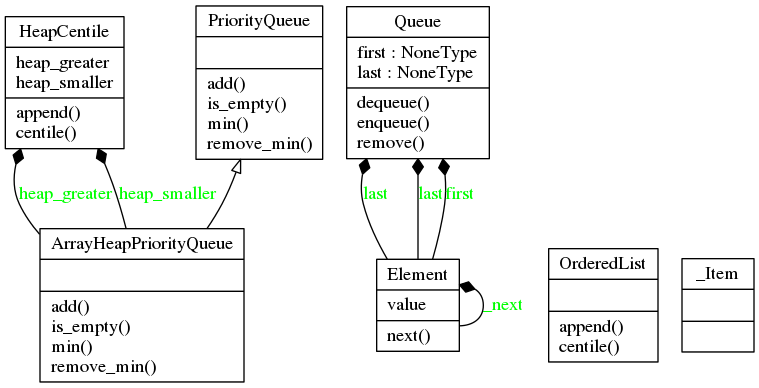
\includegraphics[resolution=130]{figures/diagramme-datastructures.png}
\end{figure}

\begin{figure}
  \centering
  \caption{Diagramme de classes du Casino.}
  \label{figure:diagramme-casino}
  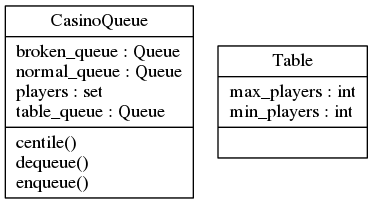
\includegraphics[resolution=130]{figures/diagramme-casino.png}
\end{figure}

\subsection{Description du fonctionnement du Casino}

\subsubsection{Classe \textsf{Queue}}

\begin{figure}
  \centering
  \label{figure:casino}
  \caption{La file du Casino est composée de trois files \textsf{Queue}.}
  \lstinputlisting[language=Python,firstline=18,lastline=38,numbers=left]{casino.py}
\end{figure}

Notre implémentation du Casino est basée sur la classe \textsf{Queue}. La file
est représentée par une liste simplement chainée. Elle respecte l'interface
\textsf{enqueue} \textsf{dequeue} et \textsf{remove}.

Elle utilise les fonctions magiques de Python pour fournir un iterable, la
longueur, l'élément suivant, l'appartenance et la valeur booléen. C'est une
approche qui facilite l'implémentation et qui favorise une utilisation simple de
la structure de donnée.

\subsubsection{Classe \textsf{CasinoQueue}}

\begin{figure}
\caption
{
  La file est implémentée avec une liste chaînée et conserve une référence vers
  le début et la fin de la liste pour \textsf{enqueue} et \textsf{dequeue} dans
  l'ordre de $O(1)$.
}
\label{figure:datastructures}
\lstinputlisting[language=Python,firstline=206,lastline=224,numbers=left]{datastructures.py}
\end{figure}

Une instance de la classe \textsf{CasinoQueue} est une file à 3 priorités.  Elle
possède les fonctions de base des files : \textsf{enqueue} et \textsf{dequeue}.
Elle possède 3 files basé sur la classe \textsf{Queue} correspondant à ses trois
priorités:
\begin{itemize}
\item table brisée ;
\item changement de table ;
\item nouveaux joueurs.
\end{itemize}

Les éléments mis dans les files sont des tuplets de joueur, table désirée et
temps d'entrée. \textsf{None} comme valeur de table signifie que le joueur ne
veut pas de table en particulier.

Lorsque appelée, la fonction \textsf{dequeue} retire, en tout respect de
l'énoncé, une personne de la file. Une exception \textsf{IndexError} est lancée
si il n'y a plus d'élément dans la file.

\textsf{dequeue} possède un ordre constant lorsque il y a des éléments
dans la queue pour table brisée et a une ordre linéaire par rapport au nombre de
joueur dans la queue pour changement de table dans tous les autres cas.

Chaque appel de la fonction \textsf{enqueue} vérifie que le nom entrée n'est pas
un doublon d'un nom existant déjà dans le casino. Si ce n'est pas le cas, les
paramètres \textsf{table} et \textsf{broken} détermineront à quelle file sera
enqueue le joueur. Une fois ajouté dans la file, le joueur est aussi ajouté à
l'ensemble des joueurs de la file pour accélérer la recherche.

Il nous aurait été possible d'implémenter la vérification des doublons par une
itération à travers les 3 files, mais cela aurait coûté une complexité d'ordre
$O(n)$. Il nous aurait été possible de faire un arbre qui stocke les noms de
tout les joueurs qui sont dans le casino et qui font des recherches en 
$O(log(n))$.

Pour cause de flemmardise, nous avons utilisé un \textsf{HashSet} (\textsf{set}
en Python) pour tester rapidement $O(1)$ l'appartenance du joueur à la file du
Casino. Le test s'effectue à travers la méthode magique
\textsf{\_\_contains\_\_} de \textsf{CasinoQueue}.

\subsubsection{Analyse empirique de \textsf{Queue}}
Tous les tests ont été exécutés sur 1000 entrées.

L'opération enqueue devrait se faire en temps constant, car la file possède une
référence vers la fin, \textsf{last}.

\begin{figure}
  \centering
  \caption{Temps d'exécution de \textsf{enqueue} en fonction du nombre d'entrée.}
  \label{figure:enqueue}
  % GNUPLOT: LaTeX picture
\setlength{\unitlength}{0.240900pt}
\ifx\plotpoint\undefined\newsavebox{\plotpoint}\fi
\sbox{\plotpoint}{\rule[-0.200pt]{0.400pt}{0.400pt}}%
\begin{picture}(1500,900)(0,0)
\sbox{\plotpoint}{\rule[-0.200pt]{0.400pt}{0.400pt}}%
\put(210.0,82.0){\rule[-0.200pt]{4.818pt}{0.400pt}}
\put(190,82){\makebox(0,0)[r]{ 0}}
\put(1419.0,82.0){\rule[-0.200pt]{4.818pt}{0.400pt}}
\put(210.0,237.0){\rule[-0.200pt]{4.818pt}{0.400pt}}
\put(190,237){\makebox(0,0)[r]{ 5e-05}}
\put(1419.0,237.0){\rule[-0.200pt]{4.818pt}{0.400pt}}
\put(210.0,393.0){\rule[-0.200pt]{4.818pt}{0.400pt}}
\put(190,393){\makebox(0,0)[r]{ 0.0001}}
\put(1419.0,393.0){\rule[-0.200pt]{4.818pt}{0.400pt}}
\put(210.0,548.0){\rule[-0.200pt]{4.818pt}{0.400pt}}
\put(190,548){\makebox(0,0)[r]{ 0.00015}}
\put(1419.0,548.0){\rule[-0.200pt]{4.818pt}{0.400pt}}
\put(210.0,704.0){\rule[-0.200pt]{4.818pt}{0.400pt}}
\put(190,704){\makebox(0,0)[r]{ 0.0002}}
\put(1419.0,704.0){\rule[-0.200pt]{4.818pt}{0.400pt}}
\put(210.0,859.0){\rule[-0.200pt]{4.818pt}{0.400pt}}
\put(190,859){\makebox(0,0)[r]{ 0.00025}}
\put(1419.0,859.0){\rule[-0.200pt]{4.818pt}{0.400pt}}
\put(210.0,82.0){\rule[-0.200pt]{0.400pt}{4.818pt}}
\put(210,41){\makebox(0,0){ 0}}
\put(210.0,839.0){\rule[-0.200pt]{0.400pt}{4.818pt}}
\put(347.0,82.0){\rule[-0.200pt]{0.400pt}{4.818pt}}
\put(347,41){\makebox(0,0){ 5000}}
\put(347.0,839.0){\rule[-0.200pt]{0.400pt}{4.818pt}}
\put(483.0,82.0){\rule[-0.200pt]{0.400pt}{4.818pt}}
\put(483,41){\makebox(0,0){ 10000}}
\put(483.0,839.0){\rule[-0.200pt]{0.400pt}{4.818pt}}
\put(620.0,82.0){\rule[-0.200pt]{0.400pt}{4.818pt}}
\put(620,41){\makebox(0,0){ 15000}}
\put(620.0,839.0){\rule[-0.200pt]{0.400pt}{4.818pt}}
\put(756.0,82.0){\rule[-0.200pt]{0.400pt}{4.818pt}}
\put(756,41){\makebox(0,0){ 20000}}
\put(756.0,839.0){\rule[-0.200pt]{0.400pt}{4.818pt}}
\put(893.0,82.0){\rule[-0.200pt]{0.400pt}{4.818pt}}
\put(893,41){\makebox(0,0){ 25000}}
\put(893.0,839.0){\rule[-0.200pt]{0.400pt}{4.818pt}}
\put(1029.0,82.0){\rule[-0.200pt]{0.400pt}{4.818pt}}
\put(1029,41){\makebox(0,0){ 30000}}
\put(1029.0,839.0){\rule[-0.200pt]{0.400pt}{4.818pt}}
\put(1166.0,82.0){\rule[-0.200pt]{0.400pt}{4.818pt}}
\put(1166,41){\makebox(0,0){ 35000}}
\put(1166.0,839.0){\rule[-0.200pt]{0.400pt}{4.818pt}}
\put(1302.0,82.0){\rule[-0.200pt]{0.400pt}{4.818pt}}
\put(1302,41){\makebox(0,0){ 40000}}
\put(1302.0,839.0){\rule[-0.200pt]{0.400pt}{4.818pt}}
\put(1439.0,82.0){\rule[-0.200pt]{0.400pt}{4.818pt}}
\put(1439,41){\makebox(0,0){ 45000}}
\put(1439.0,839.0){\rule[-0.200pt]{0.400pt}{4.818pt}}
\put(210.0,82.0){\rule[-0.200pt]{0.400pt}{187.179pt}}
\put(210.0,82.0){\rule[-0.200pt]{296.066pt}{0.400pt}}
\put(1439.0,82.0){\rule[-0.200pt]{0.400pt}{187.179pt}}
\put(210.0,859.0){\rule[-0.200pt]{296.066pt}{0.400pt}}
\put(1279,819){\makebox(0,0)[r]{"results/enqueue.plt"}}
\put(210,110){\makebox(0,0){$+$}}
\put(210,98){\makebox(0,0){$+$}}
\put(210,94){\makebox(0,0){$+$}}
\put(210,91){\makebox(0,0){$+$}}
\put(210,91){\makebox(0,0){$+$}}
\put(210,91){\makebox(0,0){$+$}}
\put(210,91){\makebox(0,0){$+$}}
\put(210,91){\makebox(0,0){$+$}}
\put(210,91){\makebox(0,0){$+$}}
\put(210,91){\makebox(0,0){$+$}}
\put(210,91){\makebox(0,0){$+$}}
\put(210,91){\makebox(0,0){$+$}}
\put(210,91){\makebox(0,0){$+$}}
\put(210,91){\makebox(0,0){$+$}}
\put(210,91){\makebox(0,0){$+$}}
\put(210,94){\makebox(0,0){$+$}}
\put(210,91){\makebox(0,0){$+$}}
\put(210,91){\makebox(0,0){$+$}}
\put(210,91){\makebox(0,0){$+$}}
\put(211,91){\makebox(0,0){$+$}}
\put(211,91){\makebox(0,0){$+$}}
\put(211,94){\makebox(0,0){$+$}}
\put(211,91){\makebox(0,0){$+$}}
\put(211,91){\makebox(0,0){$+$}}
\put(211,91){\makebox(0,0){$+$}}
\put(211,91){\makebox(0,0){$+$}}
\put(211,91){\makebox(0,0){$+$}}
\put(211,82){\makebox(0,0){$+$}}
\put(211,82){\makebox(0,0){$+$}}
\put(211,82){\makebox(0,0){$+$}}
\put(211,82){\makebox(0,0){$+$}}
\put(211,82){\makebox(0,0){$+$}}
\put(211,82){\makebox(0,0){$+$}}
\put(211,82){\makebox(0,0){$+$}}
\put(211,82){\makebox(0,0){$+$}}
\put(211,82){\makebox(0,0){$+$}}
\put(211,82){\makebox(0,0){$+$}}
\put(211,82){\makebox(0,0){$+$}}
\put(211,82){\makebox(0,0){$+$}}
\put(211,82){\makebox(0,0){$+$}}
\put(211,82){\makebox(0,0){$+$}}
\put(211,82){\makebox(0,0){$+$}}
\put(211,82){\makebox(0,0){$+$}}
\put(211,82){\makebox(0,0){$+$}}
\put(211,82){\makebox(0,0){$+$}}
\put(211,82){\makebox(0,0){$+$}}
\put(211,82){\makebox(0,0){$+$}}
\put(211,82){\makebox(0,0){$+$}}
\put(211,82){\makebox(0,0){$+$}}
\put(211,82){\makebox(0,0){$+$}}
\put(211,82){\makebox(0,0){$+$}}
\put(211,82){\makebox(0,0){$+$}}
\put(211,91){\makebox(0,0){$+$}}
\put(211,82){\makebox(0,0){$+$}}
\put(211,82){\makebox(0,0){$+$}}
\put(212,82){\makebox(0,0){$+$}}
\put(212,82){\makebox(0,0){$+$}}
\put(212,82){\makebox(0,0){$+$}}
\put(212,82){\makebox(0,0){$+$}}
\put(212,82){\makebox(0,0){$+$}}
\put(212,82){\makebox(0,0){$+$}}
\put(212,82){\makebox(0,0){$+$}}
\put(212,82){\makebox(0,0){$+$}}
\put(212,82){\makebox(0,0){$+$}}
\put(212,82){\makebox(0,0){$+$}}
\put(212,82){\makebox(0,0){$+$}}
\put(212,82){\makebox(0,0){$+$}}
\put(212,82){\makebox(0,0){$+$}}
\put(212,82){\makebox(0,0){$+$}}
\put(212,82){\makebox(0,0){$+$}}
\put(212,82){\makebox(0,0){$+$}}
\put(212,82){\makebox(0,0){$+$}}
\put(212,82){\makebox(0,0){$+$}}
\put(212,262){\makebox(0,0){$+$}}
\put(212,82){\makebox(0,0){$+$}}
\put(212,82){\makebox(0,0){$+$}}
\put(212,82){\makebox(0,0){$+$}}
\put(212,82){\makebox(0,0){$+$}}
\put(212,172){\makebox(0,0){$+$}}
\put(212,82){\makebox(0,0){$+$}}
\put(212,82){\makebox(0,0){$+$}}
\put(212,82){\makebox(0,0){$+$}}
\put(212,82){\makebox(0,0){$+$}}
\put(212,91){\makebox(0,0){$+$}}
\put(212,82){\makebox(0,0){$+$}}
\put(212,82){\makebox(0,0){$+$}}
\put(212,82){\makebox(0,0){$+$}}
\put(212,82){\makebox(0,0){$+$}}
\put(212,82){\makebox(0,0){$+$}}
\put(212,82){\makebox(0,0){$+$}}
\put(212,82){\makebox(0,0){$+$}}
\put(212,82){\makebox(0,0){$+$}}
\put(213,82){\makebox(0,0){$+$}}
\put(213,82){\makebox(0,0){$+$}}
\put(213,82){\makebox(0,0){$+$}}
\put(213,82){\makebox(0,0){$+$}}
\put(213,82){\makebox(0,0){$+$}}
\put(213,82){\makebox(0,0){$+$}}
\put(213,82){\makebox(0,0){$+$}}
\put(213,82){\makebox(0,0){$+$}}
\put(213,82){\makebox(0,0){$+$}}
\put(213,82){\makebox(0,0){$+$}}
\put(213,82){\makebox(0,0){$+$}}
\put(213,82){\makebox(0,0){$+$}}
\put(213,253){\makebox(0,0){$+$}}
\put(213,82){\makebox(0,0){$+$}}
\put(213,82){\makebox(0,0){$+$}}
\put(213,82){\makebox(0,0){$+$}}
\put(213,82){\makebox(0,0){$+$}}
\put(213,175){\makebox(0,0){$+$}}
\put(213,82){\makebox(0,0){$+$}}
\put(213,82){\makebox(0,0){$+$}}
\put(213,82){\makebox(0,0){$+$}}
\put(213,91){\makebox(0,0){$+$}}
\put(213,82){\makebox(0,0){$+$}}
\put(213,82){\makebox(0,0){$+$}}
\put(213,82){\makebox(0,0){$+$}}
\put(213,82){\makebox(0,0){$+$}}
\put(213,82){\makebox(0,0){$+$}}
\put(213,82){\makebox(0,0){$+$}}
\put(213,82){\makebox(0,0){$+$}}
\put(213,82){\makebox(0,0){$+$}}
\put(213,82){\makebox(0,0){$+$}}
\put(213,82){\makebox(0,0){$+$}}
\put(213,82){\makebox(0,0){$+$}}
\put(213,82){\makebox(0,0){$+$}}
\put(213,82){\makebox(0,0){$+$}}
\put(213,82){\makebox(0,0){$+$}}
\put(213,82){\makebox(0,0){$+$}}
\put(214,82){\makebox(0,0){$+$}}
\put(214,82){\makebox(0,0){$+$}}
\put(214,82){\makebox(0,0){$+$}}
\put(214,82){\makebox(0,0){$+$}}
\put(214,82){\makebox(0,0){$+$}}
\put(214,82){\makebox(0,0){$+$}}
\put(214,82){\makebox(0,0){$+$}}
\put(214,82){\makebox(0,0){$+$}}
\put(214,82){\makebox(0,0){$+$}}
\put(214,82){\makebox(0,0){$+$}}
\put(214,82){\makebox(0,0){$+$}}
\put(214,82){\makebox(0,0){$+$}}
\put(214,82){\makebox(0,0){$+$}}
\put(214,82){\makebox(0,0){$+$}}
\put(214,82){\makebox(0,0){$+$}}
\put(214,91){\makebox(0,0){$+$}}
\put(214,82){\makebox(0,0){$+$}}
\put(214,82){\makebox(0,0){$+$}}
\put(214,82){\makebox(0,0){$+$}}
\put(214,82){\makebox(0,0){$+$}}
\put(214,82){\makebox(0,0){$+$}}
\put(214,82){\makebox(0,0){$+$}}
\put(214,82){\makebox(0,0){$+$}}
\put(214,82){\makebox(0,0){$+$}}
\put(214,82){\makebox(0,0){$+$}}
\put(214,82){\makebox(0,0){$+$}}
\put(214,82){\makebox(0,0){$+$}}
\put(214,82){\makebox(0,0){$+$}}
\put(214,82){\makebox(0,0){$+$}}
\put(214,82){\makebox(0,0){$+$}}
\put(214,82){\makebox(0,0){$+$}}
\put(214,82){\makebox(0,0){$+$}}
\put(214,82){\makebox(0,0){$+$}}
\put(214,82){\makebox(0,0){$+$}}
\put(214,82){\makebox(0,0){$+$}}
\put(214,82){\makebox(0,0){$+$}}
\put(215,82){\makebox(0,0){$+$}}
\put(215,82){\makebox(0,0){$+$}}
\put(215,82){\makebox(0,0){$+$}}
\put(215,82){\makebox(0,0){$+$}}
\put(215,82){\makebox(0,0){$+$}}
\put(215,82){\makebox(0,0){$+$}}
\put(215,82){\makebox(0,0){$+$}}
\put(215,82){\makebox(0,0){$+$}}
\put(215,82){\makebox(0,0){$+$}}
\put(215,82){\makebox(0,0){$+$}}
\put(215,94){\makebox(0,0){$+$}}
\put(215,82){\makebox(0,0){$+$}}
\put(215,82){\makebox(0,0){$+$}}
\put(215,82){\makebox(0,0){$+$}}
\put(215,82){\makebox(0,0){$+$}}
\put(215,82){\makebox(0,0){$+$}}
\put(215,82){\makebox(0,0){$+$}}
\put(215,82){\makebox(0,0){$+$}}
\put(215,82){\makebox(0,0){$+$}}
\put(215,82){\makebox(0,0){$+$}}
\put(215,82){\makebox(0,0){$+$}}
\put(215,82){\makebox(0,0){$+$}}
\put(215,82){\makebox(0,0){$+$}}
\put(215,82){\makebox(0,0){$+$}}
\put(215,82){\makebox(0,0){$+$}}
\put(215,82){\makebox(0,0){$+$}}
\put(215,82){\makebox(0,0){$+$}}
\put(215,82){\makebox(0,0){$+$}}
\put(215,82){\makebox(0,0){$+$}}
\put(215,82){\makebox(0,0){$+$}}
\put(215,82){\makebox(0,0){$+$}}
\put(215,82){\makebox(0,0){$+$}}
\put(215,82){\makebox(0,0){$+$}}
\put(215,82){\makebox(0,0){$+$}}
\put(215,82){\makebox(0,0){$+$}}
\put(215,82){\makebox(0,0){$+$}}
\put(215,82){\makebox(0,0){$+$}}
\put(216,82){\makebox(0,0){$+$}}
\put(216,82){\makebox(0,0){$+$}}
\put(216,82){\makebox(0,0){$+$}}
\put(216,82){\makebox(0,0){$+$}}
\put(216,91){\makebox(0,0){$+$}}
\put(216,82){\makebox(0,0){$+$}}
\put(216,82){\makebox(0,0){$+$}}
\put(216,82){\makebox(0,0){$+$}}
\put(216,82){\makebox(0,0){$+$}}
\put(216,82){\makebox(0,0){$+$}}
\put(216,82){\makebox(0,0){$+$}}
\put(216,82){\makebox(0,0){$+$}}
\put(216,82){\makebox(0,0){$+$}}
\put(216,82){\makebox(0,0){$+$}}
\put(216,82){\makebox(0,0){$+$}}
\put(216,82){\makebox(0,0){$+$}}
\put(216,82){\makebox(0,0){$+$}}
\put(216,82){\makebox(0,0){$+$}}
\put(216,82){\makebox(0,0){$+$}}
\put(216,82){\makebox(0,0){$+$}}
\put(216,82){\makebox(0,0){$+$}}
\put(216,82){\makebox(0,0){$+$}}
\put(216,82){\makebox(0,0){$+$}}
\put(216,82){\makebox(0,0){$+$}}
\put(216,82){\makebox(0,0){$+$}}
\put(216,82){\makebox(0,0){$+$}}
\put(216,82){\makebox(0,0){$+$}}
\put(216,82){\makebox(0,0){$+$}}
\put(216,82){\makebox(0,0){$+$}}
\put(216,82){\makebox(0,0){$+$}}
\put(216,82){\makebox(0,0){$+$}}
\put(216,82){\makebox(0,0){$+$}}
\put(216,82){\makebox(0,0){$+$}}
\put(216,82){\makebox(0,0){$+$}}
\put(216,82){\makebox(0,0){$+$}}
\put(216,91){\makebox(0,0){$+$}}
\put(217,82){\makebox(0,0){$+$}}
\put(217,82){\makebox(0,0){$+$}}
\put(217,82){\makebox(0,0){$+$}}
\put(217,82){\makebox(0,0){$+$}}
\put(217,82){\makebox(0,0){$+$}}
\put(217,517){\makebox(0,0){$+$}}
\put(217,82){\makebox(0,0){$+$}}
\put(217,82){\makebox(0,0){$+$}}
\put(217,82){\makebox(0,0){$+$}}
\put(217,82){\makebox(0,0){$+$}}
\put(217,82){\makebox(0,0){$+$}}
\put(217,82){\makebox(0,0){$+$}}
\put(217,82){\makebox(0,0){$+$}}
\put(217,82){\makebox(0,0){$+$}}
\put(217,82){\makebox(0,0){$+$}}
\put(217,82){\makebox(0,0){$+$}}
\put(217,82){\makebox(0,0){$+$}}
\put(217,82){\makebox(0,0){$+$}}
\put(217,82){\makebox(0,0){$+$}}
\put(217,82){\makebox(0,0){$+$}}
\put(217,82){\makebox(0,0){$+$}}
\put(217,82){\makebox(0,0){$+$}}
\put(217,82){\makebox(0,0){$+$}}
\put(217,82){\makebox(0,0){$+$}}
\put(217,82){\makebox(0,0){$+$}}
\put(217,82){\makebox(0,0){$+$}}
\put(217,82){\makebox(0,0){$+$}}
\put(217,82){\makebox(0,0){$+$}}
\put(217,82){\makebox(0,0){$+$}}
\put(217,91){\makebox(0,0){$+$}}
\put(217,638){\makebox(0,0){$+$}}
\put(217,82){\makebox(0,0){$+$}}
\put(217,82){\makebox(0,0){$+$}}
\put(217,82){\makebox(0,0){$+$}}
\put(217,82){\makebox(0,0){$+$}}
\put(217,82){\makebox(0,0){$+$}}
\put(217,82){\makebox(0,0){$+$}}
\put(218,82){\makebox(0,0){$+$}}
\put(218,82){\makebox(0,0){$+$}}
\put(218,82){\makebox(0,0){$+$}}
\put(218,82){\makebox(0,0){$+$}}
\put(218,82){\makebox(0,0){$+$}}
\put(218,82){\makebox(0,0){$+$}}
\put(218,82){\makebox(0,0){$+$}}
\put(218,629){\makebox(0,0){$+$}}
\put(218,82){\makebox(0,0){$+$}}
\put(218,82){\makebox(0,0){$+$}}
\put(218,82){\makebox(0,0){$+$}}
\put(218,82){\makebox(0,0){$+$}}
\put(218,82){\makebox(0,0){$+$}}
\put(218,82){\makebox(0,0){$+$}}
\put(218,82){\makebox(0,0){$+$}}
\put(218,172){\makebox(0,0){$+$}}
\put(218,82){\makebox(0,0){$+$}}
\put(218,82){\makebox(0,0){$+$}}
\put(218,82){\makebox(0,0){$+$}}
\put(218,82){\makebox(0,0){$+$}}
\put(218,91){\makebox(0,0){$+$}}
\put(218,82){\makebox(0,0){$+$}}
\put(218,82){\makebox(0,0){$+$}}
\put(218,82){\makebox(0,0){$+$}}
\put(218,82){\makebox(0,0){$+$}}
\put(218,82){\makebox(0,0){$+$}}
\put(218,82){\makebox(0,0){$+$}}
\put(218,82){\makebox(0,0){$+$}}
\put(218,82){\makebox(0,0){$+$}}
\put(218,82){\makebox(0,0){$+$}}
\put(218,82){\makebox(0,0){$+$}}
\put(218,82){\makebox(0,0){$+$}}
\put(218,82){\makebox(0,0){$+$}}
\put(218,82){\makebox(0,0){$+$}}
\put(218,82){\makebox(0,0){$+$}}
\put(218,82){\makebox(0,0){$+$}}
\put(218,82){\makebox(0,0){$+$}}
\put(219,82){\makebox(0,0){$+$}}
\put(219,82){\makebox(0,0){$+$}}
\put(219,82){\makebox(0,0){$+$}}
\put(219,82){\makebox(0,0){$+$}}
\put(219,82){\makebox(0,0){$+$}}
\put(219,82){\makebox(0,0){$+$}}
\put(219,82){\makebox(0,0){$+$}}
\put(219,82){\makebox(0,0){$+$}}
\put(219,82){\makebox(0,0){$+$}}
\put(219,82){\makebox(0,0){$+$}}
\put(219,82){\makebox(0,0){$+$}}
\put(219,82){\makebox(0,0){$+$}}
\put(219,82){\makebox(0,0){$+$}}
\put(219,82){\makebox(0,0){$+$}}
\put(219,82){\makebox(0,0){$+$}}
\put(219,82){\makebox(0,0){$+$}}
\put(219,82){\makebox(0,0){$+$}}
\put(219,82){\makebox(0,0){$+$}}
\put(219,82){\makebox(0,0){$+$}}
\put(219,517){\makebox(0,0){$+$}}
\put(219,82){\makebox(0,0){$+$}}
\put(219,82){\makebox(0,0){$+$}}
\put(219,82){\makebox(0,0){$+$}}
\put(219,82){\makebox(0,0){$+$}}
\put(219,82){\makebox(0,0){$+$}}
\put(219,82){\makebox(0,0){$+$}}
\put(219,82){\makebox(0,0){$+$}}
\put(219,82){\makebox(0,0){$+$}}
\put(219,82){\makebox(0,0){$+$}}
\put(219,82){\makebox(0,0){$+$}}
\put(219,82){\makebox(0,0){$+$}}
\put(219,82){\makebox(0,0){$+$}}
\put(219,82){\makebox(0,0){$+$}}
\put(219,82){\makebox(0,0){$+$}}
\put(219,82){\makebox(0,0){$+$}}
\put(219,82){\makebox(0,0){$+$}}
\put(220,82){\makebox(0,0){$+$}}
\put(220,82){\makebox(0,0){$+$}}
\put(220,82){\makebox(0,0){$+$}}
\put(220,82){\makebox(0,0){$+$}}
\put(220,82){\makebox(0,0){$+$}}
\put(220,82){\makebox(0,0){$+$}}
\put(220,82){\makebox(0,0){$+$}}
\put(220,91){\makebox(0,0){$+$}}
\put(220,94){\makebox(0,0){$+$}}
\put(220,82){\makebox(0,0){$+$}}
\put(220,82){\makebox(0,0){$+$}}
\put(220,82){\makebox(0,0){$+$}}
\put(220,82){\makebox(0,0){$+$}}
\put(220,82){\makebox(0,0){$+$}}
\put(220,517){\makebox(0,0){$+$}}
\put(220,82){\makebox(0,0){$+$}}
\put(220,82){\makebox(0,0){$+$}}
\put(220,82){\makebox(0,0){$+$}}
\put(220,82){\makebox(0,0){$+$}}
\put(220,82){\makebox(0,0){$+$}}
\put(220,82){\makebox(0,0){$+$}}
\put(220,82){\makebox(0,0){$+$}}
\put(220,82){\makebox(0,0){$+$}}
\put(220,82){\makebox(0,0){$+$}}
\put(220,82){\makebox(0,0){$+$}}
\put(220,82){\makebox(0,0){$+$}}
\put(220,82){\makebox(0,0){$+$}}
\put(220,82){\makebox(0,0){$+$}}
\put(220,268){\makebox(0,0){$+$}}
\put(220,82){\makebox(0,0){$+$}}
\put(220,82){\makebox(0,0){$+$}}
\put(220,82){\makebox(0,0){$+$}}
\put(220,82){\makebox(0,0){$+$}}
\put(220,82){\makebox(0,0){$+$}}
\put(220,82){\makebox(0,0){$+$}}
\put(220,82){\makebox(0,0){$+$}}
\put(220,82){\makebox(0,0){$+$}}
\put(221,82){\makebox(0,0){$+$}}
\put(221,91){\makebox(0,0){$+$}}
\put(221,82){\makebox(0,0){$+$}}
\put(221,82){\makebox(0,0){$+$}}
\put(221,82){\makebox(0,0){$+$}}
\put(221,82){\makebox(0,0){$+$}}
\put(221,82){\makebox(0,0){$+$}}
\put(221,82){\makebox(0,0){$+$}}
\put(221,82){\makebox(0,0){$+$}}
\put(221,82){\makebox(0,0){$+$}}
\put(221,82){\makebox(0,0){$+$}}
\put(221,82){\makebox(0,0){$+$}}
\put(221,82){\makebox(0,0){$+$}}
\put(221,82){\makebox(0,0){$+$}}
\put(221,82){\makebox(0,0){$+$}}
\put(221,82){\makebox(0,0){$+$}}
\put(221,82){\makebox(0,0){$+$}}
\put(221,82){\makebox(0,0){$+$}}
\put(221,82){\makebox(0,0){$+$}}
\put(221,82){\makebox(0,0){$+$}}
\put(221,82){\makebox(0,0){$+$}}
\put(221,82){\makebox(0,0){$+$}}
\put(221,268){\makebox(0,0){$+$}}
\put(221,82){\makebox(0,0){$+$}}
\put(221,82){\makebox(0,0){$+$}}
\put(221,82){\makebox(0,0){$+$}}
\put(221,82){\makebox(0,0){$+$}}
\put(221,172){\makebox(0,0){$+$}}
\put(221,82){\makebox(0,0){$+$}}
\put(221,82){\makebox(0,0){$+$}}
\put(221,82){\makebox(0,0){$+$}}
\put(221,82){\makebox(0,0){$+$}}
\put(221,94){\makebox(0,0){$+$}}
\put(221,82){\makebox(0,0){$+$}}
\put(221,82){\makebox(0,0){$+$}}
\put(221,82){\makebox(0,0){$+$}}
\put(221,82){\makebox(0,0){$+$}}
\put(222,82){\makebox(0,0){$+$}}
\put(222,517){\makebox(0,0){$+$}}
\put(222,82){\makebox(0,0){$+$}}
\put(222,82){\makebox(0,0){$+$}}
\put(222,82){\makebox(0,0){$+$}}
\put(222,82){\makebox(0,0){$+$}}
\put(222,82){\makebox(0,0){$+$}}
\put(222,82){\makebox(0,0){$+$}}
\put(222,82){\makebox(0,0){$+$}}
\put(222,82){\makebox(0,0){$+$}}
\put(222,82){\makebox(0,0){$+$}}
\put(222,82){\makebox(0,0){$+$}}
\put(222,82){\makebox(0,0){$+$}}
\put(222,82){\makebox(0,0){$+$}}
\put(222,82){\makebox(0,0){$+$}}
\put(222,82){\makebox(0,0){$+$}}
\put(222,82){\makebox(0,0){$+$}}
\put(222,82){\makebox(0,0){$+$}}
\put(222,82){\makebox(0,0){$+$}}
\put(222,82){\makebox(0,0){$+$}}
\put(222,82){\makebox(0,0){$+$}}
\put(222,82){\makebox(0,0){$+$}}
\put(222,82){\makebox(0,0){$+$}}
\put(222,82){\makebox(0,0){$+$}}
\put(222,82){\makebox(0,0){$+$}}
\put(222,82){\makebox(0,0){$+$}}
\put(222,82){\makebox(0,0){$+$}}
\put(222,82){\makebox(0,0){$+$}}
\put(222,82){\makebox(0,0){$+$}}
\put(222,82){\makebox(0,0){$+$}}
\put(222,82){\makebox(0,0){$+$}}
\put(222,82){\makebox(0,0){$+$}}
\put(222,82){\makebox(0,0){$+$}}
\put(222,82){\makebox(0,0){$+$}}
\put(222,82){\makebox(0,0){$+$}}
\put(222,82){\makebox(0,0){$+$}}
\put(223,82){\makebox(0,0){$+$}}
\put(223,82){\makebox(0,0){$+$}}
\put(223,82){\makebox(0,0){$+$}}
\put(223,82){\makebox(0,0){$+$}}
\put(223,82){\makebox(0,0){$+$}}
\put(223,82){\makebox(0,0){$+$}}
\put(223,82){\makebox(0,0){$+$}}
\put(223,82){\makebox(0,0){$+$}}
\put(223,82){\makebox(0,0){$+$}}
\put(223,82){\makebox(0,0){$+$}}
\put(223,91){\makebox(0,0){$+$}}
\put(223,101){\makebox(0,0){$+$}}
\put(223,94){\makebox(0,0){$+$}}
\put(223,82){\makebox(0,0){$+$}}
\put(223,82){\makebox(0,0){$+$}}
\put(223,82){\makebox(0,0){$+$}}
\put(223,82){\makebox(0,0){$+$}}
\put(223,82){\makebox(0,0){$+$}}
\put(223,82){\makebox(0,0){$+$}}
\put(223,82){\makebox(0,0){$+$}}
\put(223,82){\makebox(0,0){$+$}}
\put(223,82){\makebox(0,0){$+$}}
\put(223,82){\makebox(0,0){$+$}}
\put(223,82){\makebox(0,0){$+$}}
\put(223,82){\makebox(0,0){$+$}}
\put(223,82){\makebox(0,0){$+$}}
\put(223,82){\makebox(0,0){$+$}}
\put(223,82){\makebox(0,0){$+$}}
\put(223,82){\makebox(0,0){$+$}}
\put(223,82){\makebox(0,0){$+$}}
\put(223,82){\makebox(0,0){$+$}}
\put(223,82){\makebox(0,0){$+$}}
\put(223,82){\makebox(0,0){$+$}}
\put(223,82){\makebox(0,0){$+$}}
\put(223,82){\makebox(0,0){$+$}}
\put(223,82){\makebox(0,0){$+$}}
\put(223,82){\makebox(0,0){$+$}}
\put(224,82){\makebox(0,0){$+$}}
\put(224,82){\makebox(0,0){$+$}}
\put(224,82){\makebox(0,0){$+$}}
\put(224,82){\makebox(0,0){$+$}}
\put(224,82){\makebox(0,0){$+$}}
\put(224,82){\makebox(0,0){$+$}}
\put(224,82){\makebox(0,0){$+$}}
\put(224,82){\makebox(0,0){$+$}}
\put(224,82){\makebox(0,0){$+$}}
\put(224,82){\makebox(0,0){$+$}}
\put(224,82){\makebox(0,0){$+$}}
\put(224,82){\makebox(0,0){$+$}}
\put(224,82){\makebox(0,0){$+$}}
\put(224,82){\makebox(0,0){$+$}}
\put(224,82){\makebox(0,0){$+$}}
\put(224,82){\makebox(0,0){$+$}}
\put(224,82){\makebox(0,0){$+$}}
\put(224,82){\makebox(0,0){$+$}}
\put(224,82){\makebox(0,0){$+$}}
\put(224,82){\makebox(0,0){$+$}}
\put(224,82){\makebox(0,0){$+$}}
\put(224,82){\makebox(0,0){$+$}}
\put(224,82){\makebox(0,0){$+$}}
\put(224,82){\makebox(0,0){$+$}}
\put(224,82){\makebox(0,0){$+$}}
\put(224,82){\makebox(0,0){$+$}}
\put(224,82){\makebox(0,0){$+$}}
\put(224,169){\makebox(0,0){$+$}}
\put(224,163){\makebox(0,0){$+$}}
\put(224,82){\makebox(0,0){$+$}}
\put(224,82){\makebox(0,0){$+$}}
\put(224,82){\makebox(0,0){$+$}}
\put(224,94){\makebox(0,0){$+$}}
\put(224,82){\makebox(0,0){$+$}}
\put(224,82){\makebox(0,0){$+$}}
\put(224,82){\makebox(0,0){$+$}}
\put(225,82){\makebox(0,0){$+$}}
\put(225,82){\makebox(0,0){$+$}}
\put(225,82){\makebox(0,0){$+$}}
\put(225,82){\makebox(0,0){$+$}}
\put(225,82){\makebox(0,0){$+$}}
\put(225,82){\makebox(0,0){$+$}}
\put(225,82){\makebox(0,0){$+$}}
\put(225,82){\makebox(0,0){$+$}}
\put(225,82){\makebox(0,0){$+$}}
\put(225,82){\makebox(0,0){$+$}}
\put(225,82){\makebox(0,0){$+$}}
\put(225,82){\makebox(0,0){$+$}}
\put(225,82){\makebox(0,0){$+$}}
\put(225,82){\makebox(0,0){$+$}}
\put(225,82){\makebox(0,0){$+$}}
\put(225,82){\makebox(0,0){$+$}}
\put(225,82){\makebox(0,0){$+$}}
\put(225,82){\makebox(0,0){$+$}}
\put(225,82){\makebox(0,0){$+$}}
\put(225,82){\makebox(0,0){$+$}}
\put(225,82){\makebox(0,0){$+$}}
\put(225,82){\makebox(0,0){$+$}}
\put(225,82){\makebox(0,0){$+$}}
\put(225,82){\makebox(0,0){$+$}}
\put(225,82){\makebox(0,0){$+$}}
\put(225,82){\makebox(0,0){$+$}}
\put(225,82){\makebox(0,0){$+$}}
\put(225,91){\makebox(0,0){$+$}}
\put(225,82){\makebox(0,0){$+$}}
\put(225,82){\makebox(0,0){$+$}}
\put(225,82){\makebox(0,0){$+$}}
\put(225,82){\makebox(0,0){$+$}}
\put(225,82){\makebox(0,0){$+$}}
\put(225,82){\makebox(0,0){$+$}}
\put(225,82){\makebox(0,0){$+$}}
\put(225,82){\makebox(0,0){$+$}}
\put(225,82){\makebox(0,0){$+$}}
\put(226,82){\makebox(0,0){$+$}}
\put(226,82){\makebox(0,0){$+$}}
\put(226,82){\makebox(0,0){$+$}}
\put(226,82){\makebox(0,0){$+$}}
\put(226,82){\makebox(0,0){$+$}}
\put(226,82){\makebox(0,0){$+$}}
\put(226,82){\makebox(0,0){$+$}}
\put(226,82){\makebox(0,0){$+$}}
\put(226,82){\makebox(0,0){$+$}}
\put(226,82){\makebox(0,0){$+$}}
\put(226,82){\makebox(0,0){$+$}}
\put(226,82){\makebox(0,0){$+$}}
\put(226,82){\makebox(0,0){$+$}}
\put(226,82){\makebox(0,0){$+$}}
\put(226,82){\makebox(0,0){$+$}}
\put(226,82){\makebox(0,0){$+$}}
\put(226,82){\makebox(0,0){$+$}}
\put(226,82){\makebox(0,0){$+$}}
\put(226,82){\makebox(0,0){$+$}}
\put(226,82){\makebox(0,0){$+$}}
\put(226,82){\makebox(0,0){$+$}}
\put(226,91){\makebox(0,0){$+$}}
\put(226,82){\makebox(0,0){$+$}}
\put(226,82){\makebox(0,0){$+$}}
\put(226,82){\makebox(0,0){$+$}}
\put(226,82){\makebox(0,0){$+$}}
\put(226,82){\makebox(0,0){$+$}}
\put(226,82){\makebox(0,0){$+$}}
\put(226,82){\makebox(0,0){$+$}}
\put(226,82){\makebox(0,0){$+$}}
\put(226,82){\makebox(0,0){$+$}}
\put(226,82){\makebox(0,0){$+$}}
\put(226,82){\makebox(0,0){$+$}}
\put(226,82){\makebox(0,0){$+$}}
\put(226,82){\makebox(0,0){$+$}}
\put(226,82){\makebox(0,0){$+$}}
\put(226,82){\makebox(0,0){$+$}}
\put(227,82){\makebox(0,0){$+$}}
\put(227,82){\makebox(0,0){$+$}}
\put(227,82){\makebox(0,0){$+$}}
\put(227,82){\makebox(0,0){$+$}}
\put(227,82){\makebox(0,0){$+$}}
\put(227,82){\makebox(0,0){$+$}}
\put(227,82){\makebox(0,0){$+$}}
\put(227,82){\makebox(0,0){$+$}}
\put(227,82){\makebox(0,0){$+$}}
\put(227,82){\makebox(0,0){$+$}}
\put(227,172){\makebox(0,0){$+$}}
\put(227,163){\makebox(0,0){$+$}}
\put(227,82){\makebox(0,0){$+$}}
\put(227,82){\makebox(0,0){$+$}}
\put(227,82){\makebox(0,0){$+$}}
\put(227,91){\makebox(0,0){$+$}}
\put(227,82){\makebox(0,0){$+$}}
\put(227,82){\makebox(0,0){$+$}}
\put(227,82){\makebox(0,0){$+$}}
\put(227,82){\makebox(0,0){$+$}}
\put(227,82){\makebox(0,0){$+$}}
\put(227,82){\makebox(0,0){$+$}}
\put(227,82){\makebox(0,0){$+$}}
\put(227,82){\makebox(0,0){$+$}}
\put(227,82){\makebox(0,0){$+$}}
\put(227,82){\makebox(0,0){$+$}}
\put(227,82){\makebox(0,0){$+$}}
\put(227,82){\makebox(0,0){$+$}}
\put(227,82){\makebox(0,0){$+$}}
\put(227,82){\makebox(0,0){$+$}}
\put(227,82){\makebox(0,0){$+$}}
\put(227,82){\makebox(0,0){$+$}}
\put(227,82){\makebox(0,0){$+$}}
\put(227,82){\makebox(0,0){$+$}}
\put(227,82){\makebox(0,0){$+$}}
\put(227,82){\makebox(0,0){$+$}}
\put(228,82){\makebox(0,0){$+$}}
\put(228,82){\makebox(0,0){$+$}}
\put(228,82){\makebox(0,0){$+$}}
\put(228,82){\makebox(0,0){$+$}}
\put(228,82){\makebox(0,0){$+$}}
\put(228,82){\makebox(0,0){$+$}}
\put(228,82){\makebox(0,0){$+$}}
\put(228,82){\makebox(0,0){$+$}}
\put(228,82){\makebox(0,0){$+$}}
\put(228,82){\makebox(0,0){$+$}}
\put(228,91){\makebox(0,0){$+$}}
\put(228,91){\makebox(0,0){$+$}}
\put(228,82){\makebox(0,0){$+$}}
\put(228,82){\makebox(0,0){$+$}}
\put(228,82){\makebox(0,0){$+$}}
\put(228,82){\makebox(0,0){$+$}}
\put(228,82){\makebox(0,0){$+$}}
\put(228,82){\makebox(0,0){$+$}}
\put(228,82){\makebox(0,0){$+$}}
\put(228,82){\makebox(0,0){$+$}}
\put(228,82){\makebox(0,0){$+$}}
\put(228,82){\makebox(0,0){$+$}}
\put(228,82){\makebox(0,0){$+$}}
\put(228,82){\makebox(0,0){$+$}}
\put(228,82){\makebox(0,0){$+$}}
\put(228,82){\makebox(0,0){$+$}}
\put(228,82){\makebox(0,0){$+$}}
\put(228,82){\makebox(0,0){$+$}}
\put(228,82){\makebox(0,0){$+$}}
\put(228,82){\makebox(0,0){$+$}}
\put(228,82){\makebox(0,0){$+$}}
\put(228,82){\makebox(0,0){$+$}}
\put(228,82){\makebox(0,0){$+$}}
\put(228,82){\makebox(0,0){$+$}}
\put(228,82){\makebox(0,0){$+$}}
\put(228,82){\makebox(0,0){$+$}}
\put(228,82){\makebox(0,0){$+$}}
\put(229,82){\makebox(0,0){$+$}}
\put(229,82){\makebox(0,0){$+$}}
\put(229,82){\makebox(0,0){$+$}}
\put(229,82){\makebox(0,0){$+$}}
\put(229,82){\makebox(0,0){$+$}}
\put(229,82){\makebox(0,0){$+$}}
\put(229,82){\makebox(0,0){$+$}}
\put(229,82){\makebox(0,0){$+$}}
\put(229,82){\makebox(0,0){$+$}}
\put(229,82){\makebox(0,0){$+$}}
\put(229,82){\makebox(0,0){$+$}}
\put(229,82){\makebox(0,0){$+$}}
\put(229,82){\makebox(0,0){$+$}}
\put(229,82){\makebox(0,0){$+$}}
\put(229,82){\makebox(0,0){$+$}}
\put(229,82){\makebox(0,0){$+$}}
\put(229,262){\makebox(0,0){$+$}}
\put(229,82){\makebox(0,0){$+$}}
\put(229,82){\makebox(0,0){$+$}}
\put(229,82){\makebox(0,0){$+$}}
\put(229,82){\makebox(0,0){$+$}}
\put(229,82){\makebox(0,0){$+$}}
\put(229,82){\makebox(0,0){$+$}}
\put(229,82){\makebox(0,0){$+$}}
\put(229,91){\makebox(0,0){$+$}}
\put(229,82){\makebox(0,0){$+$}}
\put(229,82){\makebox(0,0){$+$}}
\put(229,82){\makebox(0,0){$+$}}
\put(229,82){\makebox(0,0){$+$}}
\put(229,82){\makebox(0,0){$+$}}
\put(229,517){\makebox(0,0){$+$}}
\put(229,82){\makebox(0,0){$+$}}
\put(229,82){\makebox(0,0){$+$}}
\put(229,82){\makebox(0,0){$+$}}
\put(229,82){\makebox(0,0){$+$}}
\put(229,82){\makebox(0,0){$+$}}
\put(230,82){\makebox(0,0){$+$}}
\put(230,82){\makebox(0,0){$+$}}
\put(230,82){\makebox(0,0){$+$}}
\put(230,82){\makebox(0,0){$+$}}
\put(230,82){\makebox(0,0){$+$}}
\put(230,82){\makebox(0,0){$+$}}
\put(230,82){\makebox(0,0){$+$}}
\put(230,82){\makebox(0,0){$+$}}
\put(230,82){\makebox(0,0){$+$}}
\put(230,82){\makebox(0,0){$+$}}
\put(230,82){\makebox(0,0){$+$}}
\put(230,82){\makebox(0,0){$+$}}
\put(230,82){\makebox(0,0){$+$}}
\put(230,82){\makebox(0,0){$+$}}
\put(230,172){\makebox(0,0){$+$}}
\put(230,163){\makebox(0,0){$+$}}
\put(230,82){\makebox(0,0){$+$}}
\put(230,82){\makebox(0,0){$+$}}
\put(230,82){\makebox(0,0){$+$}}
\put(230,91){\makebox(0,0){$+$}}
\put(230,82){\makebox(0,0){$+$}}
\put(230,82){\makebox(0,0){$+$}}
\put(230,82){\makebox(0,0){$+$}}
\put(230,82){\makebox(0,0){$+$}}
\put(230,82){\makebox(0,0){$+$}}
\put(230,82){\makebox(0,0){$+$}}
\put(230,82){\makebox(0,0){$+$}}
\put(230,82){\makebox(0,0){$+$}}
\put(230,82){\makebox(0,0){$+$}}
\put(230,82){\makebox(0,0){$+$}}
\put(230,82){\makebox(0,0){$+$}}
\put(230,82){\makebox(0,0){$+$}}
\put(230,82){\makebox(0,0){$+$}}
\put(230,82){\makebox(0,0){$+$}}
\put(230,82){\makebox(0,0){$+$}}
\put(230,82){\makebox(0,0){$+$}}
\put(230,82){\makebox(0,0){$+$}}
\put(231,82){\makebox(0,0){$+$}}
\put(231,82){\makebox(0,0){$+$}}
\put(231,82){\makebox(0,0){$+$}}
\put(231,82){\makebox(0,0){$+$}}
\put(231,82){\makebox(0,0){$+$}}
\put(231,82){\makebox(0,0){$+$}}
\put(231,82){\makebox(0,0){$+$}}
\put(231,82){\makebox(0,0){$+$}}
\put(231,181){\makebox(0,0){$+$}}
\put(231,82){\makebox(0,0){$+$}}
\put(231,82){\makebox(0,0){$+$}}
\put(231,82){\makebox(0,0){$+$}}
\put(231,82){\makebox(0,0){$+$}}
\put(231,94){\makebox(0,0){$+$}}
\put(231,82){\makebox(0,0){$+$}}
\put(231,82){\makebox(0,0){$+$}}
\put(231,82){\makebox(0,0){$+$}}
\put(231,82){\makebox(0,0){$+$}}
\put(231,82){\makebox(0,0){$+$}}
\put(231,505){\makebox(0,0){$+$}}
\put(231,82){\makebox(0,0){$+$}}
\put(231,82){\makebox(0,0){$+$}}
\put(231,82){\makebox(0,0){$+$}}
\put(231,430){\makebox(0,0){$+$}}
\put(231,82){\makebox(0,0){$+$}}
\put(231,82){\makebox(0,0){$+$}}
\put(231,82){\makebox(0,0){$+$}}
\put(231,82){\makebox(0,0){$+$}}
\put(231,82){\makebox(0,0){$+$}}
\put(231,82){\makebox(0,0){$+$}}
\put(231,82){\makebox(0,0){$+$}}
\put(231,82){\makebox(0,0){$+$}}
\put(231,82){\makebox(0,0){$+$}}
\put(231,82){\makebox(0,0){$+$}}
\put(231,82){\makebox(0,0){$+$}}
\put(231,82){\makebox(0,0){$+$}}
\put(231,82){\makebox(0,0){$+$}}
\put(232,82){\makebox(0,0){$+$}}
\put(232,178){\makebox(0,0){$+$}}
\put(232,166){\makebox(0,0){$+$}}
\put(232,82){\makebox(0,0){$+$}}
\put(232,82){\makebox(0,0){$+$}}
\put(232,82){\makebox(0,0){$+$}}
\put(232,82){\makebox(0,0){$+$}}
\put(232,94){\makebox(0,0){$+$}}
\put(232,82){\makebox(0,0){$+$}}
\put(232,82){\makebox(0,0){$+$}}
\put(232,82){\makebox(0,0){$+$}}
\put(232,82){\makebox(0,0){$+$}}
\put(232,82){\makebox(0,0){$+$}}
\put(232,517){\makebox(0,0){$+$}}
\put(232,82){\makebox(0,0){$+$}}
\put(232,82){\makebox(0,0){$+$}}
\put(232,82){\makebox(0,0){$+$}}
\put(232,82){\makebox(0,0){$+$}}
\put(232,82){\makebox(0,0){$+$}}
\put(232,82){\makebox(0,0){$+$}}
\put(232,82){\makebox(0,0){$+$}}
\put(232,82){\makebox(0,0){$+$}}
\put(232,82){\makebox(0,0){$+$}}
\put(232,82){\makebox(0,0){$+$}}
\put(232,82){\makebox(0,0){$+$}}
\put(232,82){\makebox(0,0){$+$}}
\put(232,82){\makebox(0,0){$+$}}
\put(232,82){\makebox(0,0){$+$}}
\put(232,82){\makebox(0,0){$+$}}
\put(232,82){\makebox(0,0){$+$}}
\put(232,82){\makebox(0,0){$+$}}
\put(232,82){\makebox(0,0){$+$}}
\put(232,82){\makebox(0,0){$+$}}
\put(232,82){\makebox(0,0){$+$}}
\put(232,82){\makebox(0,0){$+$}}
\put(232,82){\makebox(0,0){$+$}}
\put(233,82){\makebox(0,0){$+$}}
\put(233,82){\makebox(0,0){$+$}}
\put(233,91){\makebox(0,0){$+$}}
\put(233,82){\makebox(0,0){$+$}}
\put(233,82){\makebox(0,0){$+$}}
\put(233,82){\makebox(0,0){$+$}}
\put(233,82){\makebox(0,0){$+$}}
\put(233,82){\makebox(0,0){$+$}}
\put(233,502){\makebox(0,0){$+$}}
\put(233,82){\makebox(0,0){$+$}}
\put(233,82){\makebox(0,0){$+$}}
\put(233,82){\makebox(0,0){$+$}}
\put(233,82){\makebox(0,0){$+$}}
\put(233,82){\makebox(0,0){$+$}}
\put(233,82){\makebox(0,0){$+$}}
\put(233,82){\makebox(0,0){$+$}}
\put(233,82){\makebox(0,0){$+$}}
\put(233,82){\makebox(0,0){$+$}}
\put(233,82){\makebox(0,0){$+$}}
\put(233,82){\makebox(0,0){$+$}}
\put(233,82){\makebox(0,0){$+$}}
\put(233,82){\makebox(0,0){$+$}}
\put(233,82){\makebox(0,0){$+$}}
\put(233,82){\makebox(0,0){$+$}}
\put(233,82){\makebox(0,0){$+$}}
\put(233,82){\makebox(0,0){$+$}}
\put(233,82){\makebox(0,0){$+$}}
\put(233,82){\makebox(0,0){$+$}}
\put(233,172){\makebox(0,0){$+$}}
\put(233,82){\makebox(0,0){$+$}}
\put(233,82){\makebox(0,0){$+$}}
\put(233,82){\makebox(0,0){$+$}}
\put(233,82){\makebox(0,0){$+$}}
\put(233,101){\makebox(0,0){$+$}}
\put(233,82){\makebox(0,0){$+$}}
\put(233,82){\makebox(0,0){$+$}}
\put(233,82){\makebox(0,0){$+$}}
\put(234,82){\makebox(0,0){$+$}}
\put(234,82){\makebox(0,0){$+$}}
\put(234,82){\makebox(0,0){$+$}}
\put(234,82){\makebox(0,0){$+$}}
\put(234,82){\makebox(0,0){$+$}}
\put(234,82){\makebox(0,0){$+$}}
\put(234,82){\makebox(0,0){$+$}}
\put(234,82){\makebox(0,0){$+$}}
\put(234,82){\makebox(0,0){$+$}}
\put(234,82){\makebox(0,0){$+$}}
\put(234,82){\makebox(0,0){$+$}}
\put(234,82){\makebox(0,0){$+$}}
\put(234,82){\makebox(0,0){$+$}}
\put(234,82){\makebox(0,0){$+$}}
\put(234,82){\makebox(0,0){$+$}}
\put(234,82){\makebox(0,0){$+$}}
\put(234,82){\makebox(0,0){$+$}}
\put(234,82){\makebox(0,0){$+$}}
\put(234,82){\makebox(0,0){$+$}}
\put(234,82){\makebox(0,0){$+$}}
\put(234,82){\makebox(0,0){$+$}}
\put(234,82){\makebox(0,0){$+$}}
\put(234,172){\makebox(0,0){$+$}}
\put(234,82){\makebox(0,0){$+$}}
\put(234,82){\makebox(0,0){$+$}}
\put(234,82){\makebox(0,0){$+$}}
\put(234,91){\makebox(0,0){$+$}}
\put(234,94){\makebox(0,0){$+$}}
\put(234,82){\makebox(0,0){$+$}}
\put(234,82){\makebox(0,0){$+$}}
\put(234,82){\makebox(0,0){$+$}}
\put(234,82){\makebox(0,0){$+$}}
\put(234,82){\makebox(0,0){$+$}}
\put(234,508){\makebox(0,0){$+$}}
\put(234,82){\makebox(0,0){$+$}}
\put(234,82){\makebox(0,0){$+$}}
\put(234,82){\makebox(0,0){$+$}}
\put(235,82){\makebox(0,0){$+$}}
\put(235,82){\makebox(0,0){$+$}}
\put(235,82){\makebox(0,0){$+$}}
\put(235,82){\makebox(0,0){$+$}}
\put(235,82){\makebox(0,0){$+$}}
\put(235,82){\makebox(0,0){$+$}}
\put(235,82){\makebox(0,0){$+$}}
\put(235,82){\makebox(0,0){$+$}}
\put(235,82){\makebox(0,0){$+$}}
\put(235,82){\makebox(0,0){$+$}}
\put(235,82){\makebox(0,0){$+$}}
\put(235,82){\makebox(0,0){$+$}}
\put(235,82){\makebox(0,0){$+$}}
\put(235,169){\makebox(0,0){$+$}}
\put(235,163){\makebox(0,0){$+$}}
\put(235,82){\makebox(0,0){$+$}}
\put(235,82){\makebox(0,0){$+$}}
\put(235,82){\makebox(0,0){$+$}}
\put(235,91){\makebox(0,0){$+$}}
\put(235,82){\makebox(0,0){$+$}}
\put(235,82){\makebox(0,0){$+$}}
\put(235,82){\makebox(0,0){$+$}}
\put(235,82){\makebox(0,0){$+$}}
\put(235,82){\makebox(0,0){$+$}}
\put(235,505){\makebox(0,0){$+$}}
\put(235,82){\makebox(0,0){$+$}}
\put(235,82){\makebox(0,0){$+$}}
\put(235,82){\makebox(0,0){$+$}}
\put(235,82){\makebox(0,0){$+$}}
\put(235,82){\makebox(0,0){$+$}}
\put(235,82){\makebox(0,0){$+$}}
\put(235,82){\makebox(0,0){$+$}}
\put(235,82){\makebox(0,0){$+$}}
\put(235,82){\makebox(0,0){$+$}}
\put(235,82){\makebox(0,0){$+$}}
\put(235,82){\makebox(0,0){$+$}}
\put(236,82){\makebox(0,0){$+$}}
\put(236,82){\makebox(0,0){$+$}}
\put(236,82){\makebox(0,0){$+$}}
\put(236,82){\makebox(0,0){$+$}}
\put(236,82){\makebox(0,0){$+$}}
\put(236,82){\makebox(0,0){$+$}}
\put(236,82){\makebox(0,0){$+$}}
\put(236,82){\makebox(0,0){$+$}}
\put(236,82){\makebox(0,0){$+$}}
\put(236,82){\makebox(0,0){$+$}}
\put(236,82){\makebox(0,0){$+$}}
\put(236,82){\makebox(0,0){$+$}}
\put(236,82){\makebox(0,0){$+$}}
\put(236,82){\makebox(0,0){$+$}}
\put(236,94){\makebox(0,0){$+$}}
\put(236,82){\makebox(0,0){$+$}}
\put(236,82){\makebox(0,0){$+$}}
\put(236,82){\makebox(0,0){$+$}}
\put(236,82){\makebox(0,0){$+$}}
\put(236,82){\makebox(0,0){$+$}}
\put(236,502){\makebox(0,0){$+$}}
\put(236,82){\makebox(0,0){$+$}}
\put(236,82){\makebox(0,0){$+$}}
\put(236,82){\makebox(0,0){$+$}}
\put(236,82){\makebox(0,0){$+$}}
\put(236,82){\makebox(0,0){$+$}}
\put(236,82){\makebox(0,0){$+$}}
\put(236,82){\makebox(0,0){$+$}}
\put(236,82){\makebox(0,0){$+$}}
\put(236,82){\makebox(0,0){$+$}}
\put(236,82){\makebox(0,0){$+$}}
\put(236,82){\makebox(0,0){$+$}}
\put(236,82){\makebox(0,0){$+$}}
\put(236,82){\makebox(0,0){$+$}}
\put(236,82){\makebox(0,0){$+$}}
\put(236,82){\makebox(0,0){$+$}}
\put(236,82){\makebox(0,0){$+$}}
\put(237,82){\makebox(0,0){$+$}}
\put(237,82){\makebox(0,0){$+$}}
\put(237,82){\makebox(0,0){$+$}}
\put(237,82){\makebox(0,0){$+$}}
\put(237,82){\makebox(0,0){$+$}}
\put(237,82){\makebox(0,0){$+$}}
\put(237,82){\makebox(0,0){$+$}}
\put(237,82){\makebox(0,0){$+$}}
\put(237,82){\makebox(0,0){$+$}}
\put(237,91){\makebox(0,0){$+$}}
\put(237,82){\makebox(0,0){$+$}}
\put(237,82){\makebox(0,0){$+$}}
\put(237,82){\makebox(0,0){$+$}}
\put(237,82){\makebox(0,0){$+$}}
\put(237,82){\makebox(0,0){$+$}}
\put(237,82){\makebox(0,0){$+$}}
\put(237,82){\makebox(0,0){$+$}}
\put(237,82){\makebox(0,0){$+$}}
\put(237,82){\makebox(0,0){$+$}}
\put(237,427){\makebox(0,0){$+$}}
\put(237,82){\makebox(0,0){$+$}}
\put(237,82){\makebox(0,0){$+$}}
\put(237,82){\makebox(0,0){$+$}}
\put(237,82){\makebox(0,0){$+$}}
\put(237,82){\makebox(0,0){$+$}}
\put(237,82){\makebox(0,0){$+$}}
\put(237,82){\makebox(0,0){$+$}}
\put(237,82){\makebox(0,0){$+$}}
\put(237,82){\makebox(0,0){$+$}}
\put(237,82){\makebox(0,0){$+$}}
\put(237,82){\makebox(0,0){$+$}}
\put(237,82){\makebox(0,0){$+$}}
\put(237,82){\makebox(0,0){$+$}}
\put(237,82){\makebox(0,0){$+$}}
\put(237,82){\makebox(0,0){$+$}}
\put(237,82){\makebox(0,0){$+$}}
\put(238,82){\makebox(0,0){$+$}}
\put(238,82){\makebox(0,0){$+$}}
\put(238,82){\makebox(0,0){$+$}}
\put(238,82){\makebox(0,0){$+$}}
\put(238,94){\makebox(0,0){$+$}}
\put(238,82){\makebox(0,0){$+$}}
\put(238,82){\makebox(0,0){$+$}}
\put(238,82){\makebox(0,0){$+$}}
\put(238,82){\makebox(0,0){$+$}}
\put(238,82){\makebox(0,0){$+$}}
\put(238,498){\makebox(0,0){$+$}}
\put(238,82){\makebox(0,0){$+$}}
\put(238,82){\makebox(0,0){$+$}}
\put(238,82){\makebox(0,0){$+$}}
\put(238,82){\makebox(0,0){$+$}}
\put(238,82){\makebox(0,0){$+$}}
\put(238,82){\makebox(0,0){$+$}}
\put(238,82){\makebox(0,0){$+$}}
\put(238,82){\makebox(0,0){$+$}}
\put(238,82){\makebox(0,0){$+$}}
\put(238,82){\makebox(0,0){$+$}}
\put(238,82){\makebox(0,0){$+$}}
\put(238,82){\makebox(0,0){$+$}}
\put(238,82){\makebox(0,0){$+$}}
\put(238,82){\makebox(0,0){$+$}}
\put(238,82){\makebox(0,0){$+$}}
\put(238,82){\makebox(0,0){$+$}}
\put(238,82){\makebox(0,0){$+$}}
\put(238,82){\makebox(0,0){$+$}}
\put(238,82){\makebox(0,0){$+$}}
\put(238,175){\makebox(0,0){$+$}}
\put(238,82){\makebox(0,0){$+$}}
\put(238,82){\makebox(0,0){$+$}}
\put(238,82){\makebox(0,0){$+$}}
\put(238,82){\makebox(0,0){$+$}}
\put(238,94){\makebox(0,0){$+$}}
\put(238,82){\makebox(0,0){$+$}}
\put(239,82){\makebox(0,0){$+$}}
\put(239,82){\makebox(0,0){$+$}}
\put(239,82){\makebox(0,0){$+$}}
\put(239,82){\makebox(0,0){$+$}}
\put(239,82){\makebox(0,0){$+$}}
\put(239,82){\makebox(0,0){$+$}}
\put(239,82){\makebox(0,0){$+$}}
\put(239,82){\makebox(0,0){$+$}}
\put(239,82){\makebox(0,0){$+$}}
\put(239,82){\makebox(0,0){$+$}}
\put(239,82){\makebox(0,0){$+$}}
\put(239,82){\makebox(0,0){$+$}}
\put(239,82){\makebox(0,0){$+$}}
\put(239,82){\makebox(0,0){$+$}}
\put(239,82){\makebox(0,0){$+$}}
\put(239,82){\makebox(0,0){$+$}}
\put(239,82){\makebox(0,0){$+$}}
\put(239,82){\makebox(0,0){$+$}}
\put(239,82){\makebox(0,0){$+$}}
\put(239,82){\makebox(0,0){$+$}}
\put(239,82){\makebox(0,0){$+$}}
\put(239,82){\makebox(0,0){$+$}}
\put(239,91){\makebox(0,0){$+$}}
\put(239,82){\makebox(0,0){$+$}}
\put(239,82){\makebox(0,0){$+$}}
\put(239,82){\makebox(0,0){$+$}}
\put(239,82){\makebox(0,0){$+$}}
\put(239,82){\makebox(0,0){$+$}}
\put(239,82){\makebox(0,0){$+$}}
\put(239,82){\makebox(0,0){$+$}}
\put(239,82){\makebox(0,0){$+$}}
\put(239,82){\makebox(0,0){$+$}}
\put(239,82){\makebox(0,0){$+$}}
\put(239,82){\makebox(0,0){$+$}}
\put(239,82){\makebox(0,0){$+$}}
\put(239,82){\makebox(0,0){$+$}}
\put(239,368){\makebox(0,0){$+$}}
\put(240,82){\makebox(0,0){$+$}}
\put(240,82){\makebox(0,0){$+$}}
\put(240,82){\makebox(0,0){$+$}}
\put(240,82){\makebox(0,0){$+$}}
\put(240,281){\makebox(0,0){$+$}}
\put(240,82){\makebox(0,0){$+$}}
\put(240,82){\makebox(0,0){$+$}}
\put(240,82){\makebox(0,0){$+$}}
\put(240,82){\makebox(0,0){$+$}}
\put(240,178){\makebox(0,0){$+$}}
\put(240,169){\makebox(0,0){$+$}}
\put(240,82){\makebox(0,0){$+$}}
\put(240,82){\makebox(0,0){$+$}}
\put(240,82){\makebox(0,0){$+$}}
\put(240,91){\makebox(0,0){$+$}}
\put(240,94){\makebox(0,0){$+$}}
\put(240,82){\makebox(0,0){$+$}}
\put(240,82){\makebox(0,0){$+$}}
\put(240,82){\makebox(0,0){$+$}}
\put(240,82){\makebox(0,0){$+$}}
\put(240,82){\makebox(0,0){$+$}}
\put(240,82){\makebox(0,0){$+$}}
\put(240,82){\makebox(0,0){$+$}}
\put(240,82){\makebox(0,0){$+$}}
\put(240,82){\makebox(0,0){$+$}}
\put(240,82){\makebox(0,0){$+$}}
\put(240,82){\makebox(0,0){$+$}}
\put(240,82){\makebox(0,0){$+$}}
\put(240,82){\makebox(0,0){$+$}}
\put(240,82){\makebox(0,0){$+$}}
\put(240,82){\makebox(0,0){$+$}}
\put(240,82){\makebox(0,0){$+$}}
\put(240,82){\makebox(0,0){$+$}}
\put(240,82){\makebox(0,0){$+$}}
\put(240,82){\makebox(0,0){$+$}}
\put(240,82){\makebox(0,0){$+$}}
\put(241,82){\makebox(0,0){$+$}}
\put(241,175){\makebox(0,0){$+$}}
\put(241,160){\makebox(0,0){$+$}}
\put(241,82){\makebox(0,0){$+$}}
\put(241,82){\makebox(0,0){$+$}}
\put(241,82){\makebox(0,0){$+$}}
\put(241,91){\makebox(0,0){$+$}}
\put(241,82){\makebox(0,0){$+$}}
\put(241,82){\makebox(0,0){$+$}}
\put(241,82){\makebox(0,0){$+$}}
\put(241,82){\makebox(0,0){$+$}}
\put(241,82){\makebox(0,0){$+$}}
\put(241,82){\makebox(0,0){$+$}}
\put(241,82){\makebox(0,0){$+$}}
\put(241,82){\makebox(0,0){$+$}}
\put(241,82){\makebox(0,0){$+$}}
\put(241,82){\makebox(0,0){$+$}}
\put(241,82){\makebox(0,0){$+$}}
\put(241,82){\makebox(0,0){$+$}}
\put(241,82){\makebox(0,0){$+$}}
\put(241,82){\makebox(0,0){$+$}}
\put(241,82){\makebox(0,0){$+$}}
\put(241,82){\makebox(0,0){$+$}}
\put(241,82){\makebox(0,0){$+$}}
\put(241,82){\makebox(0,0){$+$}}
\put(241,82){\makebox(0,0){$+$}}
\put(241,82){\makebox(0,0){$+$}}
\put(241,82){\makebox(0,0){$+$}}
\put(241,82){\makebox(0,0){$+$}}
\put(241,82){\makebox(0,0){$+$}}
\put(241,82){\makebox(0,0){$+$}}
\put(241,82){\makebox(0,0){$+$}}
\put(241,175){\makebox(0,0){$+$}}
\put(241,166){\makebox(0,0){$+$}}
\put(241,82){\makebox(0,0){$+$}}
\put(241,82){\makebox(0,0){$+$}}
\put(241,82){\makebox(0,0){$+$}}
\put(242,91){\makebox(0,0){$+$}}
\put(242,82){\makebox(0,0){$+$}}
\put(242,82){\makebox(0,0){$+$}}
\put(242,82){\makebox(0,0){$+$}}
\put(242,82){\makebox(0,0){$+$}}
\put(242,82){\makebox(0,0){$+$}}
\put(242,82){\makebox(0,0){$+$}}
\put(242,82){\makebox(0,0){$+$}}
\put(242,82){\makebox(0,0){$+$}}
\put(242,82){\makebox(0,0){$+$}}
\put(242,82){\makebox(0,0){$+$}}
\put(242,82){\makebox(0,0){$+$}}
\put(242,82){\makebox(0,0){$+$}}
\put(242,82){\makebox(0,0){$+$}}
\put(242,82){\makebox(0,0){$+$}}
\put(242,82){\makebox(0,0){$+$}}
\put(242,82){\makebox(0,0){$+$}}
\put(242,82){\makebox(0,0){$+$}}
\put(242,82){\makebox(0,0){$+$}}
\put(242,82){\makebox(0,0){$+$}}
\put(242,272){\makebox(0,0){$+$}}
\put(242,82){\makebox(0,0){$+$}}
\put(242,82){\makebox(0,0){$+$}}
\put(242,82){\makebox(0,0){$+$}}
\put(242,82){\makebox(0,0){$+$}}
\put(242,82){\makebox(0,0){$+$}}
\put(242,82){\makebox(0,0){$+$}}
\put(242,82){\makebox(0,0){$+$}}
\put(242,82){\makebox(0,0){$+$}}
\put(242,82){\makebox(0,0){$+$}}
\put(242,82){\makebox(0,0){$+$}}
\put(242,94){\makebox(0,0){$+$}}
\put(242,82){\makebox(0,0){$+$}}
\put(242,82){\makebox(0,0){$+$}}
\put(242,82){\makebox(0,0){$+$}}
\put(242,82){\makebox(0,0){$+$}}
\put(243,82){\makebox(0,0){$+$}}
\put(243,82){\makebox(0,0){$+$}}
\put(243,82){\makebox(0,0){$+$}}
\put(243,82){\makebox(0,0){$+$}}
\put(243,82){\makebox(0,0){$+$}}
\put(243,82){\makebox(0,0){$+$}}
\put(243,82){\makebox(0,0){$+$}}
\put(243,82){\makebox(0,0){$+$}}
\put(243,82){\makebox(0,0){$+$}}
\put(243,82){\makebox(0,0){$+$}}
\put(243,82){\makebox(0,0){$+$}}
\put(243,82){\makebox(0,0){$+$}}
\put(243,82){\makebox(0,0){$+$}}
\put(243,82){\makebox(0,0){$+$}}
\put(243,82){\makebox(0,0){$+$}}
\put(243,82){\makebox(0,0){$+$}}
\put(243,82){\makebox(0,0){$+$}}
\put(243,82){\makebox(0,0){$+$}}
\put(243,82){\makebox(0,0){$+$}}
\put(243,82){\makebox(0,0){$+$}}
\put(243,82){\makebox(0,0){$+$}}
\put(243,82){\makebox(0,0){$+$}}
\put(243,82){\makebox(0,0){$+$}}
\put(243,82){\makebox(0,0){$+$}}
\put(243,82){\makebox(0,0){$+$}}
\put(243,82){\makebox(0,0){$+$}}
\put(243,91){\makebox(0,0){$+$}}
\put(243,82){\makebox(0,0){$+$}}
\put(243,82){\makebox(0,0){$+$}}
\put(243,82){\makebox(0,0){$+$}}
\put(243,82){\makebox(0,0){$+$}}
\put(243,82){\makebox(0,0){$+$}}
\put(243,82){\makebox(0,0){$+$}}
\put(243,82){\makebox(0,0){$+$}}
\put(243,82){\makebox(0,0){$+$}}
\put(243,82){\makebox(0,0){$+$}}
\put(243,82){\makebox(0,0){$+$}}
\put(244,82){\makebox(0,0){$+$}}
\put(244,82){\makebox(0,0){$+$}}
\put(244,82){\makebox(0,0){$+$}}
\put(244,82){\makebox(0,0){$+$}}
\put(244,82){\makebox(0,0){$+$}}
\put(244,82){\makebox(0,0){$+$}}
\put(244,82){\makebox(0,0){$+$}}
\put(244,82){\makebox(0,0){$+$}}
\put(244,82){\makebox(0,0){$+$}}
\put(244,82){\makebox(0,0){$+$}}
\put(244,82){\makebox(0,0){$+$}}
\put(244,82){\makebox(0,0){$+$}}
\put(244,82){\makebox(0,0){$+$}}
\put(244,82){\makebox(0,0){$+$}}
\put(244,82){\makebox(0,0){$+$}}
\put(244,82){\makebox(0,0){$+$}}
\put(244,82){\makebox(0,0){$+$}}
\put(244,82){\makebox(0,0){$+$}}
\put(244,82){\makebox(0,0){$+$}}
\put(244,91){\makebox(0,0){$+$}}
\put(244,94){\makebox(0,0){$+$}}
\put(244,82){\makebox(0,0){$+$}}
\put(244,82){\makebox(0,0){$+$}}
\put(244,82){\makebox(0,0){$+$}}
\put(244,82){\makebox(0,0){$+$}}
\put(244,82){\makebox(0,0){$+$}}
\put(244,82){\makebox(0,0){$+$}}
\put(244,82){\makebox(0,0){$+$}}
\put(244,82){\makebox(0,0){$+$}}
\put(244,82){\makebox(0,0){$+$}}
\put(244,82){\makebox(0,0){$+$}}
\put(244,82){\makebox(0,0){$+$}}
\put(244,82){\makebox(0,0){$+$}}
\put(244,82){\makebox(0,0){$+$}}
\put(244,82){\makebox(0,0){$+$}}
\put(244,82){\makebox(0,0){$+$}}
\put(244,82){\makebox(0,0){$+$}}
\put(245,82){\makebox(0,0){$+$}}
\put(245,82){\makebox(0,0){$+$}}
\put(245,82){\makebox(0,0){$+$}}
\put(245,82){\makebox(0,0){$+$}}
\put(245,82){\makebox(0,0){$+$}}
\put(245,82){\makebox(0,0){$+$}}
\put(245,82){\makebox(0,0){$+$}}
\put(245,82){\makebox(0,0){$+$}}
\put(245,181){\makebox(0,0){$+$}}
\put(245,163){\makebox(0,0){$+$}}
\put(245,82){\makebox(0,0){$+$}}
\put(245,82){\makebox(0,0){$+$}}
\put(245,82){\makebox(0,0){$+$}}
\put(245,82){\makebox(0,0){$+$}}
\put(245,91){\makebox(0,0){$+$}}
\put(245,82){\makebox(0,0){$+$}}
\put(245,82){\makebox(0,0){$+$}}
\put(245,82){\makebox(0,0){$+$}}
\put(245,82){\makebox(0,0){$+$}}
\put(245,82){\makebox(0,0){$+$}}
\put(245,82){\makebox(0,0){$+$}}
\put(245,82){\makebox(0,0){$+$}}
\put(245,82){\makebox(0,0){$+$}}
\put(245,82){\makebox(0,0){$+$}}
\put(245,82){\makebox(0,0){$+$}}
\put(245,82){\makebox(0,0){$+$}}
\put(245,82){\makebox(0,0){$+$}}
\put(245,82){\makebox(0,0){$+$}}
\put(245,82){\makebox(0,0){$+$}}
\put(245,82){\makebox(0,0){$+$}}
\put(245,82){\makebox(0,0){$+$}}
\put(245,82){\makebox(0,0){$+$}}
\put(245,82){\makebox(0,0){$+$}}
\put(245,82){\makebox(0,0){$+$}}
\put(245,82){\makebox(0,0){$+$}}
\put(245,82){\makebox(0,0){$+$}}
\put(246,82){\makebox(0,0){$+$}}
\put(246,82){\makebox(0,0){$+$}}
\put(246,82){\makebox(0,0){$+$}}
\put(246,82){\makebox(0,0){$+$}}
\put(246,82){\makebox(0,0){$+$}}
\put(246,82){\makebox(0,0){$+$}}
\put(246,91){\makebox(0,0){$+$}}
\put(246,82){\makebox(0,0){$+$}}
\put(246,82){\makebox(0,0){$+$}}
\put(246,82){\makebox(0,0){$+$}}
\put(246,82){\makebox(0,0){$+$}}
\put(246,82){\makebox(0,0){$+$}}
\put(246,82){\makebox(0,0){$+$}}
\put(246,82){\makebox(0,0){$+$}}
\put(246,82){\makebox(0,0){$+$}}
\put(246,82){\makebox(0,0){$+$}}
\put(246,82){\makebox(0,0){$+$}}
\put(246,82){\makebox(0,0){$+$}}
\put(246,82){\makebox(0,0){$+$}}
\put(246,82){\makebox(0,0){$+$}}
\put(246,82){\makebox(0,0){$+$}}
\put(246,82){\makebox(0,0){$+$}}
\put(246,82){\makebox(0,0){$+$}}
\put(246,82){\makebox(0,0){$+$}}
\put(246,82){\makebox(0,0){$+$}}
\put(246,82){\makebox(0,0){$+$}}
\put(246,82){\makebox(0,0){$+$}}
\put(246,82){\makebox(0,0){$+$}}
\put(246,82){\makebox(0,0){$+$}}
\put(246,82){\makebox(0,0){$+$}}
\put(246,82){\makebox(0,0){$+$}}
\put(246,82){\makebox(0,0){$+$}}
\put(246,82){\makebox(0,0){$+$}}
\put(246,82){\makebox(0,0){$+$}}
\put(246,82){\makebox(0,0){$+$}}
\put(246,82){\makebox(0,0){$+$}}
\put(246,82){\makebox(0,0){$+$}}
\put(247,91){\makebox(0,0){$+$}}
\put(247,82){\makebox(0,0){$+$}}
\put(247,82){\makebox(0,0){$+$}}
\put(247,82){\makebox(0,0){$+$}}
\put(247,82){\makebox(0,0){$+$}}
\put(247,82){\makebox(0,0){$+$}}
\put(247,82){\makebox(0,0){$+$}}
\put(247,82){\makebox(0,0){$+$}}
\put(247,82){\makebox(0,0){$+$}}
\put(247,82){\makebox(0,0){$+$}}
\put(247,418){\makebox(0,0){$+$}}
\put(247,82){\makebox(0,0){$+$}}
\put(247,82){\makebox(0,0){$+$}}
\put(247,82){\makebox(0,0){$+$}}
\put(247,82){\makebox(0,0){$+$}}
\put(247,82){\makebox(0,0){$+$}}
\put(247,82){\makebox(0,0){$+$}}
\put(247,82){\makebox(0,0){$+$}}
\put(247,82){\makebox(0,0){$+$}}
\put(247,82){\makebox(0,0){$+$}}
\put(247,82){\makebox(0,0){$+$}}
\put(247,82){\makebox(0,0){$+$}}
\put(247,82){\makebox(0,0){$+$}}
\put(247,82){\makebox(0,0){$+$}}
\put(247,82){\makebox(0,0){$+$}}
\put(247,82){\makebox(0,0){$+$}}
\put(247,82){\makebox(0,0){$+$}}
\put(247,172){\makebox(0,0){$+$}}
\put(247,82){\makebox(0,0){$+$}}
\put(247,82){\makebox(0,0){$+$}}
\put(247,82){\makebox(0,0){$+$}}
\put(247,82){\makebox(0,0){$+$}}
\put(247,91){\makebox(0,0){$+$}}
\put(247,82){\makebox(0,0){$+$}}
\put(247,82){\makebox(0,0){$+$}}
\put(247,82){\makebox(0,0){$+$}}
\put(247,82){\makebox(0,0){$+$}}
\put(248,82){\makebox(0,0){$+$}}
\put(248,82){\makebox(0,0){$+$}}
\put(248,82){\makebox(0,0){$+$}}
\put(248,82){\makebox(0,0){$+$}}
\put(248,82){\makebox(0,0){$+$}}
\put(248,415){\makebox(0,0){$+$}}
\put(248,82){\makebox(0,0){$+$}}
\put(248,82){\makebox(0,0){$+$}}
\put(248,82){\makebox(0,0){$+$}}
\put(248,82){\makebox(0,0){$+$}}
\put(248,82){\makebox(0,0){$+$}}
\put(248,82){\makebox(0,0){$+$}}
\put(248,82){\makebox(0,0){$+$}}
\put(248,82){\makebox(0,0){$+$}}
\put(248,82){\makebox(0,0){$+$}}
\put(248,82){\makebox(0,0){$+$}}
\put(248,82){\makebox(0,0){$+$}}
\put(248,82){\makebox(0,0){$+$}}
\put(248,82){\makebox(0,0){$+$}}
\put(248,163){\makebox(0,0){$+$}}
\put(248,82){\makebox(0,0){$+$}}
\put(248,94){\makebox(0,0){$+$}}
\put(248,82){\makebox(0,0){$+$}}
\put(248,82){\makebox(0,0){$+$}}
\put(248,82){\makebox(0,0){$+$}}
\put(248,82){\makebox(0,0){$+$}}
\put(248,82){\makebox(0,0){$+$}}
\put(248,82){\makebox(0,0){$+$}}
\put(248,82){\makebox(0,0){$+$}}
\put(248,82){\makebox(0,0){$+$}}
\put(248,411){\makebox(0,0){$+$}}
\put(248,82){\makebox(0,0){$+$}}
\put(248,82){\makebox(0,0){$+$}}
\put(248,82){\makebox(0,0){$+$}}
\put(248,82){\makebox(0,0){$+$}}
\put(248,82){\makebox(0,0){$+$}}
\put(249,82){\makebox(0,0){$+$}}
\put(249,82){\makebox(0,0){$+$}}
\put(249,82){\makebox(0,0){$+$}}
\put(249,82){\makebox(0,0){$+$}}
\put(249,82){\makebox(0,0){$+$}}
\put(249,82){\makebox(0,0){$+$}}
\put(249,82){\makebox(0,0){$+$}}
\put(249,82){\makebox(0,0){$+$}}
\put(249,82){\makebox(0,0){$+$}}
\put(249,178){\makebox(0,0){$+$}}
\put(249,163){\makebox(0,0){$+$}}
\put(249,82){\makebox(0,0){$+$}}
\put(249,82){\makebox(0,0){$+$}}
\put(249,82){\makebox(0,0){$+$}}
\put(249,82){\makebox(0,0){$+$}}
\put(249,94){\makebox(0,0){$+$}}
\put(249,82){\makebox(0,0){$+$}}
\put(249,82){\makebox(0,0){$+$}}
\put(249,82){\makebox(0,0){$+$}}
\put(249,82){\makebox(0,0){$+$}}
\put(249,82){\makebox(0,0){$+$}}
\put(249,82){\makebox(0,0){$+$}}
\put(249,82){\makebox(0,0){$+$}}
\put(249,82){\makebox(0,0){$+$}}
\put(249,82){\makebox(0,0){$+$}}
\put(249,82){\makebox(0,0){$+$}}
\put(249,82){\makebox(0,0){$+$}}
\put(249,82){\makebox(0,0){$+$}}
\put(249,82){\makebox(0,0){$+$}}
\put(249,82){\makebox(0,0){$+$}}
\put(249,82){\makebox(0,0){$+$}}
\put(249,82){\makebox(0,0){$+$}}
\put(249,82){\makebox(0,0){$+$}}
\put(249,82){\makebox(0,0){$+$}}
\put(249,265){\makebox(0,0){$+$}}
\put(249,82){\makebox(0,0){$+$}}
\put(249,244){\makebox(0,0){$+$}}
\put(250,82){\makebox(0,0){$+$}}
\put(250,82){\makebox(0,0){$+$}}
\put(250,82){\makebox(0,0){$+$}}
\put(250,82){\makebox(0,0){$+$}}
\put(250,82){\makebox(0,0){$+$}}
\put(250,82){\makebox(0,0){$+$}}
\put(250,82){\makebox(0,0){$+$}}
\put(250,82){\makebox(0,0){$+$}}
\put(250,82){\makebox(0,0){$+$}}
\put(250,91){\makebox(0,0){$+$}}
\put(250,82){\makebox(0,0){$+$}}
\put(250,82){\makebox(0,0){$+$}}
\put(250,82){\makebox(0,0){$+$}}
\put(250,82){\makebox(0,0){$+$}}
\put(250,82){\makebox(0,0){$+$}}
\put(250,82){\makebox(0,0){$+$}}
\put(250,82){\makebox(0,0){$+$}}
\put(250,82){\makebox(0,0){$+$}}
\put(250,82){\makebox(0,0){$+$}}
\put(250,82){\makebox(0,0){$+$}}
\put(250,82){\makebox(0,0){$+$}}
\put(250,82){\makebox(0,0){$+$}}
\put(250,82){\makebox(0,0){$+$}}
\put(250,82){\makebox(0,0){$+$}}
\put(250,82){\makebox(0,0){$+$}}
\put(250,82){\makebox(0,0){$+$}}
\put(250,82){\makebox(0,0){$+$}}
\put(250,82){\makebox(0,0){$+$}}
\put(250,82){\makebox(0,0){$+$}}
\put(250,82){\makebox(0,0){$+$}}
\put(250,82){\makebox(0,0){$+$}}
\put(250,82){\makebox(0,0){$+$}}
\put(250,82){\makebox(0,0){$+$}}
\put(250,82){\makebox(0,0){$+$}}
\put(250,82){\makebox(0,0){$+$}}
\put(250,82){\makebox(0,0){$+$}}
\put(251,82){\makebox(0,0){$+$}}
\put(251,82){\makebox(0,0){$+$}}
\put(251,82){\makebox(0,0){$+$}}
\put(251,82){\makebox(0,0){$+$}}
\put(251,91){\makebox(0,0){$+$}}
\put(251,573){\makebox(0,0){$+$}}
\put(251,82){\makebox(0,0){$+$}}
\put(251,82){\makebox(0,0){$+$}}
\put(251,82){\makebox(0,0){$+$}}
\put(251,82){\makebox(0,0){$+$}}
\put(251,82){\makebox(0,0){$+$}}
\put(251,82){\makebox(0,0){$+$}}
\put(251,82){\makebox(0,0){$+$}}
\put(251,82){\makebox(0,0){$+$}}
\put(251,82){\makebox(0,0){$+$}}
\put(251,82){\makebox(0,0){$+$}}
\put(251,82){\makebox(0,0){$+$}}
\put(251,82){\makebox(0,0){$+$}}
\put(251,82){\makebox(0,0){$+$}}
\put(251,82){\makebox(0,0){$+$}}
\put(251,82){\makebox(0,0){$+$}}
\put(251,82){\makebox(0,0){$+$}}
\put(251,82){\makebox(0,0){$+$}}
\put(251,82){\makebox(0,0){$+$}}
\put(251,82){\makebox(0,0){$+$}}
\put(251,94){\makebox(0,0){$+$}}
\put(251,82){\makebox(0,0){$+$}}
\put(251,82){\makebox(0,0){$+$}}
\put(251,82){\makebox(0,0){$+$}}
\put(251,82){\makebox(0,0){$+$}}
\put(251,82){\makebox(0,0){$+$}}
\put(251,82){\makebox(0,0){$+$}}
\put(251,82){\makebox(0,0){$+$}}
\put(251,82){\makebox(0,0){$+$}}
\put(251,82){\makebox(0,0){$+$}}
\put(251,82){\makebox(0,0){$+$}}
\put(251,82){\makebox(0,0){$+$}}
\put(252,82){\makebox(0,0){$+$}}
\put(252,82){\makebox(0,0){$+$}}
\put(252,82){\makebox(0,0){$+$}}
\put(252,82){\makebox(0,0){$+$}}
\put(252,82){\makebox(0,0){$+$}}
\put(252,82){\makebox(0,0){$+$}}
\put(252,82){\makebox(0,0){$+$}}
\put(252,82){\makebox(0,0){$+$}}
\put(252,82){\makebox(0,0){$+$}}
\put(252,82){\makebox(0,0){$+$}}
\put(252,82){\makebox(0,0){$+$}}
\put(252,82){\makebox(0,0){$+$}}
\put(252,82){\makebox(0,0){$+$}}
\put(252,82){\makebox(0,0){$+$}}
\put(252,82){\makebox(0,0){$+$}}
\put(252,82){\makebox(0,0){$+$}}
\put(252,82){\makebox(0,0){$+$}}
\put(252,82){\makebox(0,0){$+$}}
\put(252,82){\makebox(0,0){$+$}}
\put(252,82){\makebox(0,0){$+$}}
\put(252,91){\makebox(0,0){$+$}}
\put(252,82){\makebox(0,0){$+$}}
\put(252,82){\makebox(0,0){$+$}}
\put(252,82){\makebox(0,0){$+$}}
\put(252,82){\makebox(0,0){$+$}}
\put(252,82){\makebox(0,0){$+$}}
\put(252,82){\makebox(0,0){$+$}}
\put(252,82){\makebox(0,0){$+$}}
\put(252,82){\makebox(0,0){$+$}}
\put(252,82){\makebox(0,0){$+$}}
\put(252,82){\makebox(0,0){$+$}}
\put(252,82){\makebox(0,0){$+$}}
\put(252,82){\makebox(0,0){$+$}}
\put(252,82){\makebox(0,0){$+$}}
\put(252,82){\makebox(0,0){$+$}}
\put(252,82){\makebox(0,0){$+$}}
\put(252,82){\makebox(0,0){$+$}}
\put(253,82){\makebox(0,0){$+$}}
\put(253,82){\makebox(0,0){$+$}}
\put(253,82){\makebox(0,0){$+$}}
\put(253,82){\makebox(0,0){$+$}}
\put(253,82){\makebox(0,0){$+$}}
\put(253,82){\makebox(0,0){$+$}}
\put(253,82){\makebox(0,0){$+$}}
\put(253,82){\makebox(0,0){$+$}}
\put(253,82){\makebox(0,0){$+$}}
\put(253,82){\makebox(0,0){$+$}}
\put(253,82){\makebox(0,0){$+$}}
\put(253,82){\makebox(0,0){$+$}}
\put(253,82){\makebox(0,0){$+$}}
\put(253,82){\makebox(0,0){$+$}}
\put(253,91){\makebox(0,0){$+$}}
\put(253,82){\makebox(0,0){$+$}}
\put(253,82){\makebox(0,0){$+$}}
\put(253,82){\makebox(0,0){$+$}}
\put(253,82){\makebox(0,0){$+$}}
\put(253,82){\makebox(0,0){$+$}}
\put(253,82){\makebox(0,0){$+$}}
\put(253,82){\makebox(0,0){$+$}}
\put(253,82){\makebox(0,0){$+$}}
\put(253,82){\makebox(0,0){$+$}}
\put(253,82){\makebox(0,0){$+$}}
\put(253,82){\makebox(0,0){$+$}}
\put(253,82){\makebox(0,0){$+$}}
\put(253,82){\makebox(0,0){$+$}}
\put(253,82){\makebox(0,0){$+$}}
\put(253,82){\makebox(0,0){$+$}}
\put(253,82){\makebox(0,0){$+$}}
\put(253,82){\makebox(0,0){$+$}}
\put(253,82){\makebox(0,0){$+$}}
\put(253,82){\makebox(0,0){$+$}}
\put(253,82){\makebox(0,0){$+$}}
\put(253,82){\makebox(0,0){$+$}}
\put(254,82){\makebox(0,0){$+$}}
\put(254,82){\makebox(0,0){$+$}}
\put(254,82){\makebox(0,0){$+$}}
\put(254,82){\makebox(0,0){$+$}}
\put(254,82){\makebox(0,0){$+$}}
\put(254,82){\makebox(0,0){$+$}}
\put(254,82){\makebox(0,0){$+$}}
\put(254,82){\makebox(0,0){$+$}}
\put(254,82){\makebox(0,0){$+$}}
\put(254,82){\makebox(0,0){$+$}}
\put(254,94){\makebox(0,0){$+$}}
\put(254,82){\makebox(0,0){$+$}}
\put(254,82){\makebox(0,0){$+$}}
\put(254,82){\makebox(0,0){$+$}}
\put(254,82){\makebox(0,0){$+$}}
\put(254,82){\makebox(0,0){$+$}}
\put(254,82){\makebox(0,0){$+$}}
\put(254,82){\makebox(0,0){$+$}}
\put(254,82){\makebox(0,0){$+$}}
\put(254,82){\makebox(0,0){$+$}}
\put(254,82){\makebox(0,0){$+$}}
\put(254,82){\makebox(0,0){$+$}}
\put(254,82){\makebox(0,0){$+$}}
\put(254,82){\makebox(0,0){$+$}}
\put(254,82){\makebox(0,0){$+$}}
\put(254,82){\makebox(0,0){$+$}}
\put(254,82){\makebox(0,0){$+$}}
\put(254,82){\makebox(0,0){$+$}}
\put(254,82){\makebox(0,0){$+$}}
\put(254,82){\makebox(0,0){$+$}}
\put(254,82){\makebox(0,0){$+$}}
\put(254,82){\makebox(0,0){$+$}}
\put(254,82){\makebox(0,0){$+$}}
\put(254,82){\makebox(0,0){$+$}}
\put(254,82){\makebox(0,0){$+$}}
\put(254,172){\makebox(0,0){$+$}}
\put(254,166){\makebox(0,0){$+$}}
\put(255,82){\makebox(0,0){$+$}}
\put(255,82){\makebox(0,0){$+$}}
\put(255,82){\makebox(0,0){$+$}}
\put(255,82){\makebox(0,0){$+$}}
\put(255,91){\makebox(0,0){$+$}}
\put(255,82){\makebox(0,0){$+$}}
\put(255,82){\makebox(0,0){$+$}}
\put(255,82){\makebox(0,0){$+$}}
\put(255,82){\makebox(0,0){$+$}}
\put(255,82){\makebox(0,0){$+$}}
\put(255,82){\makebox(0,0){$+$}}
\put(255,82){\makebox(0,0){$+$}}
\put(255,82){\makebox(0,0){$+$}}
\put(255,82){\makebox(0,0){$+$}}
\put(255,82){\makebox(0,0){$+$}}
\put(255,82){\makebox(0,0){$+$}}
\put(255,82){\makebox(0,0){$+$}}
\put(255,352){\makebox(0,0){$+$}}
\put(255,82){\makebox(0,0){$+$}}
\put(255,82){\makebox(0,0){$+$}}
\put(255,82){\makebox(0,0){$+$}}
\put(255,82){\makebox(0,0){$+$}}
\put(255,268){\makebox(0,0){$+$}}
\put(255,82){\makebox(0,0){$+$}}
\put(255,250){\makebox(0,0){$+$}}
\put(255,82){\makebox(0,0){$+$}}
\put(255,82){\makebox(0,0){$+$}}
\put(255,82){\makebox(0,0){$+$}}
\put(255,82){\makebox(0,0){$+$}}
\put(255,175){\makebox(0,0){$+$}}
\put(255,82){\makebox(0,0){$+$}}
\put(255,82){\makebox(0,0){$+$}}
\put(255,82){\makebox(0,0){$+$}}
\put(255,82){\makebox(0,0){$+$}}
\put(255,82){\makebox(0,0){$+$}}
\put(255,82){\makebox(0,0){$+$}}
\put(256,82){\makebox(0,0){$+$}}
\put(256,82){\makebox(0,0){$+$}}
\put(256,82){\makebox(0,0){$+$}}
\put(256,82){\makebox(0,0){$+$}}
\put(256,82){\makebox(0,0){$+$}}
\put(256,82){\makebox(0,0){$+$}}
\put(256,82){\makebox(0,0){$+$}}
\put(256,82){\makebox(0,0){$+$}}
\put(256,82){\makebox(0,0){$+$}}
\put(256,82){\makebox(0,0){$+$}}
\put(256,82){\makebox(0,0){$+$}}
\put(256,82){\makebox(0,0){$+$}}
\put(256,82){\makebox(0,0){$+$}}
\put(256,82){\makebox(0,0){$+$}}
\put(256,82){\makebox(0,0){$+$}}
\put(256,82){\makebox(0,0){$+$}}
\put(256,82){\makebox(0,0){$+$}}
\put(256,188){\makebox(0,0){$+$}}
\put(256,82){\makebox(0,0){$+$}}
\put(256,82){\makebox(0,0){$+$}}
\put(256,82){\makebox(0,0){$+$}}
\put(256,91){\makebox(0,0){$+$}}
\put(256,82){\makebox(0,0){$+$}}
\put(256,82){\makebox(0,0){$+$}}
\put(256,82){\makebox(0,0){$+$}}
\put(256,82){\makebox(0,0){$+$}}
\put(256,82){\makebox(0,0){$+$}}
\put(256,82){\makebox(0,0){$+$}}
\put(256,82){\makebox(0,0){$+$}}
\put(256,82){\makebox(0,0){$+$}}
\put(256,82){\makebox(0,0){$+$}}
\put(256,82){\makebox(0,0){$+$}}
\put(256,82){\makebox(0,0){$+$}}
\put(256,362){\makebox(0,0){$+$}}
\put(256,82){\makebox(0,0){$+$}}
\put(256,281){\makebox(0,0){$+$}}
\put(256,82){\makebox(0,0){$+$}}
\put(257,82){\makebox(0,0){$+$}}
\put(257,82){\makebox(0,0){$+$}}
\put(257,82){\makebox(0,0){$+$}}
\put(257,82){\makebox(0,0){$+$}}
\put(257,82){\makebox(0,0){$+$}}
\put(257,82){\makebox(0,0){$+$}}
\put(257,175){\makebox(0,0){$+$}}
\put(257,82){\makebox(0,0){$+$}}
\put(257,82){\makebox(0,0){$+$}}
\put(257,82){\makebox(0,0){$+$}}
\put(257,82){\makebox(0,0){$+$}}
\put(257,82){\makebox(0,0){$+$}}
\put(257,82){\makebox(0,0){$+$}}
\put(257,82){\makebox(0,0){$+$}}
\put(257,82){\makebox(0,0){$+$}}
\put(257,82){\makebox(0,0){$+$}}
\put(257,82){\makebox(0,0){$+$}}
\put(257,82){\makebox(0,0){$+$}}
\put(257,82){\makebox(0,0){$+$}}
\put(257,82){\makebox(0,0){$+$}}
\put(257,82){\makebox(0,0){$+$}}
\put(257,82){\makebox(0,0){$+$}}
\put(257,82){\makebox(0,0){$+$}}
\put(257,82){\makebox(0,0){$+$}}
\put(257,352){\makebox(0,0){$+$}}
\put(257,82){\makebox(0,0){$+$}}
\put(257,82){\makebox(0,0){$+$}}
\put(257,82){\makebox(0,0){$+$}}
\put(257,82){\makebox(0,0){$+$}}
\put(257,82){\makebox(0,0){$+$}}
\put(257,82){\makebox(0,0){$+$}}
\put(257,82){\makebox(0,0){$+$}}
\put(257,82){\makebox(0,0){$+$}}
\put(257,82){\makebox(0,0){$+$}}
\put(257,82){\makebox(0,0){$+$}}
\put(257,82){\makebox(0,0){$+$}}
\put(257,82){\makebox(0,0){$+$}}
\put(258,172){\makebox(0,0){$+$}}
\put(258,82){\makebox(0,0){$+$}}
\put(258,82){\makebox(0,0){$+$}}
\put(258,82){\makebox(0,0){$+$}}
\put(258,82){\makebox(0,0){$+$}}
\put(258,82){\makebox(0,0){$+$}}
\put(258,558){\makebox(0,0){$+$}}
\put(258,82){\makebox(0,0){$+$}}
\put(258,82){\makebox(0,0){$+$}}
\put(258,467){\makebox(0,0){$+$}}
\put(258,82){\makebox(0,0){$+$}}
\put(258,82){\makebox(0,0){$+$}}
\put(258,82){\makebox(0,0){$+$}}
\put(258,415){\makebox(0,0){$+$}}
\put(258,82){\makebox(0,0){$+$}}
\put(258,82){\makebox(0,0){$+$}}
\put(258,82){\makebox(0,0){$+$}}
\put(258,82){\makebox(0,0){$+$}}
\put(258,82){\makebox(0,0){$+$}}
\put(258,82){\makebox(0,0){$+$}}
\put(258,82){\makebox(0,0){$+$}}
\put(258,82){\makebox(0,0){$+$}}
\put(258,82){\makebox(0,0){$+$}}
\put(258,82){\makebox(0,0){$+$}}
\put(258,82){\makebox(0,0){$+$}}
\put(258,82){\makebox(0,0){$+$}}
\put(258,82){\makebox(0,0){$+$}}
\put(258,82){\makebox(0,0){$+$}}
\put(258,82){\makebox(0,0){$+$}}
\put(258,82){\makebox(0,0){$+$}}
\put(258,82){\makebox(0,0){$+$}}
\put(258,82){\makebox(0,0){$+$}}
\put(258,82){\makebox(0,0){$+$}}
\put(258,91){\makebox(0,0){$+$}}
\put(258,82){\makebox(0,0){$+$}}
\put(258,82){\makebox(0,0){$+$}}
\put(259,82){\makebox(0,0){$+$}}
\put(259,82){\makebox(0,0){$+$}}
\put(259,82){\makebox(0,0){$+$}}
\put(259,82){\makebox(0,0){$+$}}
\put(259,82){\makebox(0,0){$+$}}
\put(259,82){\makebox(0,0){$+$}}
\put(259,82){\makebox(0,0){$+$}}
\put(259,82){\makebox(0,0){$+$}}
\put(259,82){\makebox(0,0){$+$}}
\put(259,343){\makebox(0,0){$+$}}
\put(259,82){\makebox(0,0){$+$}}
\put(259,82){\makebox(0,0){$+$}}
\put(259,82){\makebox(0,0){$+$}}
\put(259,82){\makebox(0,0){$+$}}
\put(259,82){\makebox(0,0){$+$}}
\put(259,82){\makebox(0,0){$+$}}
\put(259,82){\makebox(0,0){$+$}}
\put(259,82){\makebox(0,0){$+$}}
\put(259,82){\makebox(0,0){$+$}}
\put(259,82){\makebox(0,0){$+$}}
\put(259,82){\makebox(0,0){$+$}}
\put(259,82){\makebox(0,0){$+$}}
\put(259,82){\makebox(0,0){$+$}}
\put(259,82){\makebox(0,0){$+$}}
\put(259,82){\makebox(0,0){$+$}}
\put(259,94){\makebox(0,0){$+$}}
\put(259,82){\makebox(0,0){$+$}}
\put(259,82){\makebox(0,0){$+$}}
\put(259,82){\makebox(0,0){$+$}}
\put(259,82){\makebox(0,0){$+$}}
\put(259,82){\makebox(0,0){$+$}}
\put(259,82){\makebox(0,0){$+$}}
\put(259,82){\makebox(0,0){$+$}}
\put(259,82){\makebox(0,0){$+$}}
\put(259,82){\makebox(0,0){$+$}}
\put(259,82){\makebox(0,0){$+$}}
\put(259,82){\makebox(0,0){$+$}}
\put(260,82){\makebox(0,0){$+$}}
\put(260,82){\makebox(0,0){$+$}}
\put(260,82){\makebox(0,0){$+$}}
\put(260,82){\makebox(0,0){$+$}}
\put(260,82){\makebox(0,0){$+$}}
\put(260,82){\makebox(0,0){$+$}}
\put(260,82){\makebox(0,0){$+$}}
\put(260,82){\makebox(0,0){$+$}}
\put(260,82){\makebox(0,0){$+$}}
\put(260,82){\makebox(0,0){$+$}}
\put(260,82){\makebox(0,0){$+$}}
\put(260,82){\makebox(0,0){$+$}}
\put(260,82){\makebox(0,0){$+$}}
\put(260,82){\makebox(0,0){$+$}}
\put(260,82){\makebox(0,0){$+$}}
\put(260,82){\makebox(0,0){$+$}}
\put(260,82){\makebox(0,0){$+$}}
\put(260,82){\makebox(0,0){$+$}}
\put(260,82){\makebox(0,0){$+$}}
\put(260,91){\makebox(0,0){$+$}}
\put(260,82){\makebox(0,0){$+$}}
\put(260,82){\makebox(0,0){$+$}}
\put(260,82){\makebox(0,0){$+$}}
\put(260,82){\makebox(0,0){$+$}}
\put(260,82){\makebox(0,0){$+$}}
\put(260,82){\makebox(0,0){$+$}}
\put(260,82){\makebox(0,0){$+$}}
\put(260,82){\makebox(0,0){$+$}}
\put(260,82){\makebox(0,0){$+$}}
\put(260,82){\makebox(0,0){$+$}}
\put(260,82){\makebox(0,0){$+$}}
\put(260,82){\makebox(0,0){$+$}}
\put(260,352){\makebox(0,0){$+$}}
\put(260,82){\makebox(0,0){$+$}}
\put(260,82){\makebox(0,0){$+$}}
\put(260,82){\makebox(0,0){$+$}}
\put(260,82){\makebox(0,0){$+$}}
\put(261,82){\makebox(0,0){$+$}}
\put(261,82){\makebox(0,0){$+$}}
\put(261,82){\makebox(0,0){$+$}}
\put(261,82){\makebox(0,0){$+$}}
\put(261,82){\makebox(0,0){$+$}}
\put(261,82){\makebox(0,0){$+$}}
\put(261,82){\makebox(0,0){$+$}}
\put(261,82){\makebox(0,0){$+$}}
\put(261,82){\makebox(0,0){$+$}}
\put(261,82){\makebox(0,0){$+$}}
\put(261,82){\makebox(0,0){$+$}}
\put(261,82){\makebox(0,0){$+$}}
\put(261,82){\makebox(0,0){$+$}}
\put(261,91){\makebox(0,0){$+$}}
\put(261,548){\makebox(0,0){$+$}}
\put(261,82){\makebox(0,0){$+$}}
\put(261,82){\makebox(0,0){$+$}}
\put(261,82){\makebox(0,0){$+$}}
\put(261,82){\makebox(0,0){$+$}}
\put(261,82){\makebox(0,0){$+$}}
\put(261,82){\makebox(0,0){$+$}}
\put(261,82){\makebox(0,0){$+$}}
\put(261,82){\makebox(0,0){$+$}}
\put(261,82){\makebox(0,0){$+$}}
\put(261,82){\makebox(0,0){$+$}}
\put(261,82){\makebox(0,0){$+$}}
\put(261,349){\makebox(0,0){$+$}}
\put(261,82){\makebox(0,0){$+$}}
\put(261,82){\makebox(0,0){$+$}}
\put(261,82){\makebox(0,0){$+$}}
\put(261,82){\makebox(0,0){$+$}}
\put(261,82){\makebox(0,0){$+$}}
\put(261,82){\makebox(0,0){$+$}}
\put(261,82){\makebox(0,0){$+$}}
\put(261,82){\makebox(0,0){$+$}}
\put(261,82){\makebox(0,0){$+$}}
\put(262,82){\makebox(0,0){$+$}}
\put(262,82){\makebox(0,0){$+$}}
\put(262,82){\makebox(0,0){$+$}}
\put(262,82){\makebox(0,0){$+$}}
\put(262,82){\makebox(0,0){$+$}}
\put(262,82){\makebox(0,0){$+$}}
\put(262,82){\makebox(0,0){$+$}}
\put(262,82){\makebox(0,0){$+$}}
\put(262,352){\makebox(0,0){$+$}}
\put(262,82){\makebox(0,0){$+$}}
\put(262,82){\makebox(0,0){$+$}}
\put(262,82){\makebox(0,0){$+$}}
\put(262,82){\makebox(0,0){$+$}}
\put(262,82){\makebox(0,0){$+$}}
\put(262,82){\makebox(0,0){$+$}}
\put(262,82){\makebox(0,0){$+$}}
\put(262,82){\makebox(0,0){$+$}}
\put(262,82){\makebox(0,0){$+$}}
\put(262,82){\makebox(0,0){$+$}}
\put(262,82){\makebox(0,0){$+$}}
\put(262,82){\makebox(0,0){$+$}}
\put(262,82){\makebox(0,0){$+$}}
\put(262,82){\makebox(0,0){$+$}}
\put(262,91){\makebox(0,0){$+$}}
\put(262,545){\makebox(0,0){$+$}}
\put(262,82){\makebox(0,0){$+$}}
\put(262,82){\makebox(0,0){$+$}}
\put(262,82){\makebox(0,0){$+$}}
\put(262,82){\makebox(0,0){$+$}}
\put(262,82){\makebox(0,0){$+$}}
\put(262,82){\makebox(0,0){$+$}}
\put(262,82){\makebox(0,0){$+$}}
\put(262,82){\makebox(0,0){$+$}}
\put(262,82){\makebox(0,0){$+$}}
\put(262,82){\makebox(0,0){$+$}}
\put(262,82){\makebox(0,0){$+$}}
\put(262,82){\makebox(0,0){$+$}}
\put(263,82){\makebox(0,0){$+$}}
\put(263,82){\makebox(0,0){$+$}}
\put(263,82){\makebox(0,0){$+$}}
\put(263,82){\makebox(0,0){$+$}}
\put(263,82){\makebox(0,0){$+$}}
\put(263,82){\makebox(0,0){$+$}}
\put(263,82){\makebox(0,0){$+$}}
\put(263,82){\makebox(0,0){$+$}}
\put(263,82){\makebox(0,0){$+$}}
\put(263,82){\makebox(0,0){$+$}}
\put(263,82){\makebox(0,0){$+$}}
\put(263,82){\makebox(0,0){$+$}}
\put(263,82){\makebox(0,0){$+$}}
\put(263,82){\makebox(0,0){$+$}}
\put(263,82){\makebox(0,0){$+$}}
\put(263,82){\makebox(0,0){$+$}}
\put(263,82){\makebox(0,0){$+$}}
\put(263,82){\makebox(0,0){$+$}}
\put(263,91){\makebox(0,0){$+$}}
\put(263,82){\makebox(0,0){$+$}}
\put(263,82){\makebox(0,0){$+$}}
\put(263,82){\makebox(0,0){$+$}}
\put(263,82){\makebox(0,0){$+$}}
\put(263,82){\makebox(0,0){$+$}}
\put(263,82){\makebox(0,0){$+$}}
\put(263,82){\makebox(0,0){$+$}}
\put(263,82){\makebox(0,0){$+$}}
\put(263,82){\makebox(0,0){$+$}}
\put(263,82){\makebox(0,0){$+$}}
\put(263,82){\makebox(0,0){$+$}}
\put(263,82){\makebox(0,0){$+$}}
\put(263,343){\makebox(0,0){$+$}}
\put(263,82){\makebox(0,0){$+$}}
\put(263,82){\makebox(0,0){$+$}}
\put(263,82){\makebox(0,0){$+$}}
\put(263,82){\makebox(0,0){$+$}}
\put(264,82){\makebox(0,0){$+$}}
\put(264,82){\makebox(0,0){$+$}}
\put(264,82){\makebox(0,0){$+$}}
\put(264,82){\makebox(0,0){$+$}}
\put(264,82){\makebox(0,0){$+$}}
\put(264,82){\makebox(0,0){$+$}}
\put(264,82){\makebox(0,0){$+$}}
\put(264,82){\makebox(0,0){$+$}}
\put(264,82){\makebox(0,0){$+$}}
\put(264,82){\makebox(0,0){$+$}}
\put(264,82){\makebox(0,0){$+$}}
\put(264,82){\makebox(0,0){$+$}}
\put(264,82){\makebox(0,0){$+$}}
\put(264,82){\makebox(0,0){$+$}}
\put(264,536){\makebox(0,0){$+$}}
\put(264,82){\makebox(0,0){$+$}}
\put(264,82){\makebox(0,0){$+$}}
\put(264,82){\makebox(0,0){$+$}}
\put(264,82){\makebox(0,0){$+$}}
\put(264,82){\makebox(0,0){$+$}}
\put(264,82){\makebox(0,0){$+$}}
\put(264,82){\makebox(0,0){$+$}}
\put(264,82){\makebox(0,0){$+$}}
\put(264,82){\makebox(0,0){$+$}}
\put(264,82){\makebox(0,0){$+$}}
\put(264,82){\makebox(0,0){$+$}}
\put(264,346){\makebox(0,0){$+$}}
\put(264,82){\makebox(0,0){$+$}}
\put(264,82){\makebox(0,0){$+$}}
\put(264,82){\makebox(0,0){$+$}}
\put(264,82){\makebox(0,0){$+$}}
\put(264,82){\makebox(0,0){$+$}}
\put(264,82){\makebox(0,0){$+$}}
\put(264,82){\makebox(0,0){$+$}}
\put(264,82){\makebox(0,0){$+$}}
\put(264,82){\makebox(0,0){$+$}}
\put(264,82){\makebox(0,0){$+$}}
\put(265,82){\makebox(0,0){$+$}}
\put(265,82){\makebox(0,0){$+$}}
\put(265,175){\makebox(0,0){$+$}}
\put(265,163){\makebox(0,0){$+$}}
\put(265,82){\makebox(0,0){$+$}}
\put(265,82){\makebox(0,0){$+$}}
\put(265,82){\makebox(0,0){$+$}}
\put(265,82){\makebox(0,0){$+$}}
\put(265,94){\makebox(0,0){$+$}}
\put(265,82){\makebox(0,0){$+$}}
\put(265,82){\makebox(0,0){$+$}}
\put(265,82){\makebox(0,0){$+$}}
\put(265,82){\makebox(0,0){$+$}}
\put(265,82){\makebox(0,0){$+$}}
\put(265,82){\makebox(0,0){$+$}}
\put(265,82){\makebox(0,0){$+$}}
\put(265,82){\makebox(0,0){$+$}}
\put(265,82){\makebox(0,0){$+$}}
\put(265,82){\makebox(0,0){$+$}}
\put(265,82){\makebox(0,0){$+$}}
\put(265,82){\makebox(0,0){$+$}}
\put(265,82){\makebox(0,0){$+$}}
\put(265,82){\makebox(0,0){$+$}}
\put(265,82){\makebox(0,0){$+$}}
\put(265,82){\makebox(0,0){$+$}}
\put(265,82){\makebox(0,0){$+$}}
\put(265,82){\makebox(0,0){$+$}}
\put(265,82){\makebox(0,0){$+$}}
\put(265,82){\makebox(0,0){$+$}}
\put(265,82){\makebox(0,0){$+$}}
\put(265,82){\makebox(0,0){$+$}}
\put(265,82){\makebox(0,0){$+$}}
\put(265,82){\makebox(0,0){$+$}}
\put(265,82){\makebox(0,0){$+$}}
\put(265,82){\makebox(0,0){$+$}}
\put(265,82){\makebox(0,0){$+$}}
\put(265,82){\makebox(0,0){$+$}}
\put(266,82){\makebox(0,0){$+$}}
\put(266,82){\makebox(0,0){$+$}}
\put(266,94){\makebox(0,0){$+$}}
\put(266,536){\makebox(0,0){$+$}}
\put(266,82){\makebox(0,0){$+$}}
\put(266,82){\makebox(0,0){$+$}}
\put(266,82){\makebox(0,0){$+$}}
\put(266,82){\makebox(0,0){$+$}}
\put(266,82){\makebox(0,0){$+$}}
\put(266,82){\makebox(0,0){$+$}}
\put(266,82){\makebox(0,0){$+$}}
\put(266,82){\makebox(0,0){$+$}}
\put(266,82){\makebox(0,0){$+$}}
\put(266,82){\makebox(0,0){$+$}}
\put(266,82){\makebox(0,0){$+$}}
\put(266,82){\makebox(0,0){$+$}}
\put(266,82){\makebox(0,0){$+$}}
\put(266,82){\makebox(0,0){$+$}}
\put(266,82){\makebox(0,0){$+$}}
\put(266,82){\makebox(0,0){$+$}}
\put(266,82){\makebox(0,0){$+$}}
\put(266,82){\makebox(0,0){$+$}}
\put(266,82){\makebox(0,0){$+$}}
\put(266,82){\makebox(0,0){$+$}}
\put(266,82){\makebox(0,0){$+$}}
\put(266,82){\makebox(0,0){$+$}}
\put(266,82){\makebox(0,0){$+$}}
\put(266,82){\makebox(0,0){$+$}}
\put(266,82){\makebox(0,0){$+$}}
\put(266,82){\makebox(0,0){$+$}}
\put(266,82){\makebox(0,0){$+$}}
\put(266,82){\makebox(0,0){$+$}}
\put(266,82){\makebox(0,0){$+$}}
\put(266,91){\makebox(0,0){$+$}}
\put(266,82){\makebox(0,0){$+$}}
\put(266,82){\makebox(0,0){$+$}}
\put(267,82){\makebox(0,0){$+$}}
\put(267,82){\makebox(0,0){$+$}}
\put(267,446){\makebox(0,0){$+$}}
\put(267,82){\makebox(0,0){$+$}}
\put(267,82){\makebox(0,0){$+$}}
\put(267,82){\makebox(0,0){$+$}}
\put(267,82){\makebox(0,0){$+$}}
\put(267,82){\makebox(0,0){$+$}}
\put(267,82){\makebox(0,0){$+$}}
\put(267,346){\makebox(0,0){$+$}}
\put(267,82){\makebox(0,0){$+$}}
\put(267,82){\makebox(0,0){$+$}}
\put(267,82){\makebox(0,0){$+$}}
\put(267,82){\makebox(0,0){$+$}}
\put(267,82){\makebox(0,0){$+$}}
\put(267,82){\makebox(0,0){$+$}}
\put(267,82){\makebox(0,0){$+$}}
\put(267,82){\makebox(0,0){$+$}}
\put(267,82){\makebox(0,0){$+$}}
\put(267,82){\makebox(0,0){$+$}}
\put(267,82){\makebox(0,0){$+$}}
\put(267,82){\makebox(0,0){$+$}}
\put(267,175){\makebox(0,0){$+$}}
\put(267,82){\makebox(0,0){$+$}}
\put(267,82){\makebox(0,0){$+$}}
\put(267,82){\makebox(0,0){$+$}}
\put(267,82){\makebox(0,0){$+$}}
\put(267,82){\makebox(0,0){$+$}}
\put(267,91){\makebox(0,0){$+$}}
\put(267,82){\makebox(0,0){$+$}}
\put(267,82){\makebox(0,0){$+$}}
\put(267,82){\makebox(0,0){$+$}}
\put(267,82){\makebox(0,0){$+$}}
\put(267,82){\makebox(0,0){$+$}}
\put(267,82){\makebox(0,0){$+$}}
\put(267,82){\makebox(0,0){$+$}}
\put(267,82){\makebox(0,0){$+$}}
\put(268,82){\makebox(0,0){$+$}}
\put(268,82){\makebox(0,0){$+$}}
\put(268,82){\makebox(0,0){$+$}}
\put(268,82){\makebox(0,0){$+$}}
\put(268,82){\makebox(0,0){$+$}}
\put(268,82){\makebox(0,0){$+$}}
\put(268,82){\makebox(0,0){$+$}}
\put(268,82){\makebox(0,0){$+$}}
\put(268,82){\makebox(0,0){$+$}}
\put(268,82){\makebox(0,0){$+$}}
\put(268,82){\makebox(0,0){$+$}}
\put(268,82){\makebox(0,0){$+$}}
\put(268,82){\makebox(0,0){$+$}}
\put(268,82){\makebox(0,0){$+$}}
\put(268,82){\makebox(0,0){$+$}}
\put(268,82){\makebox(0,0){$+$}}
\put(268,82){\makebox(0,0){$+$}}
\put(268,82){\makebox(0,0){$+$}}
\put(268,82){\makebox(0,0){$+$}}
\put(268,91){\makebox(0,0){$+$}}
\put(268,82){\makebox(0,0){$+$}}
\put(268,82){\makebox(0,0){$+$}}
\put(268,82){\makebox(0,0){$+$}}
\put(268,82){\makebox(0,0){$+$}}
\put(268,82){\makebox(0,0){$+$}}
\put(268,82){\makebox(0,0){$+$}}
\put(268,82){\makebox(0,0){$+$}}
\put(268,82){\makebox(0,0){$+$}}
\put(268,82){\makebox(0,0){$+$}}
\put(268,82){\makebox(0,0){$+$}}
\put(268,82){\makebox(0,0){$+$}}
\put(268,82){\makebox(0,0){$+$}}
\put(268,346){\makebox(0,0){$+$}}
\put(268,82){\makebox(0,0){$+$}}
\put(268,82){\makebox(0,0){$+$}}
\put(268,82){\makebox(0,0){$+$}}
\put(269,82){\makebox(0,0){$+$}}
\put(269,82){\makebox(0,0){$+$}}
\put(269,82){\makebox(0,0){$+$}}
\put(269,82){\makebox(0,0){$+$}}
\put(269,82){\makebox(0,0){$+$}}
\put(269,82){\makebox(0,0){$+$}}
\put(269,82){\makebox(0,0){$+$}}
\put(269,82){\makebox(0,0){$+$}}
\put(269,82){\makebox(0,0){$+$}}
\put(269,82){\makebox(0,0){$+$}}
\put(269,82){\makebox(0,0){$+$}}
\put(269,82){\makebox(0,0){$+$}}
\put(269,82){\makebox(0,0){$+$}}
\put(269,82){\makebox(0,0){$+$}}
\put(269,94){\makebox(0,0){$+$}}
\put(269,533){\makebox(0,0){$+$}}
\put(269,82){\makebox(0,0){$+$}}
\put(269,82){\makebox(0,0){$+$}}
\put(269,82){\makebox(0,0){$+$}}
\put(269,82){\makebox(0,0){$+$}}
\put(269,82){\makebox(0,0){$+$}}
\put(269,82){\makebox(0,0){$+$}}
\put(269,82){\makebox(0,0){$+$}}
\put(269,82){\makebox(0,0){$+$}}
\put(269,82){\makebox(0,0){$+$}}
\put(269,82){\makebox(0,0){$+$}}
\put(269,82){\makebox(0,0){$+$}}
\put(269,349){\makebox(0,0){$+$}}
\put(269,82){\makebox(0,0){$+$}}
\put(269,82){\makebox(0,0){$+$}}
\put(269,82){\makebox(0,0){$+$}}
\put(269,82){\makebox(0,0){$+$}}
\put(269,82){\makebox(0,0){$+$}}
\put(269,82){\makebox(0,0){$+$}}
\put(269,82){\makebox(0,0){$+$}}
\put(269,82){\makebox(0,0){$+$}}
\put(269,82){\makebox(0,0){$+$}}
\put(270,82){\makebox(0,0){$+$}}
\put(270,82){\makebox(0,0){$+$}}
\put(270,82){\makebox(0,0){$+$}}
\put(270,82){\makebox(0,0){$+$}}
\put(270,82){\makebox(0,0){$+$}}
\put(270,82){\makebox(0,0){$+$}}
\put(270,82){\makebox(0,0){$+$}}
\put(270,82){\makebox(0,0){$+$}}
\put(270,82){\makebox(0,0){$+$}}
\put(270,94){\makebox(0,0){$+$}}
\put(270,82){\makebox(0,0){$+$}}
\put(270,82){\makebox(0,0){$+$}}
\put(270,82){\makebox(0,0){$+$}}
\put(270,82){\makebox(0,0){$+$}}
\put(270,433){\makebox(0,0){$+$}}
\put(270,82){\makebox(0,0){$+$}}
\put(270,82){\makebox(0,0){$+$}}
\put(270,82){\makebox(0,0){$+$}}
\put(270,82){\makebox(0,0){$+$}}
\put(270,82){\makebox(0,0){$+$}}
\put(270,82){\makebox(0,0){$+$}}
\put(270,349){\makebox(0,0){$+$}}
\put(270,82){\makebox(0,0){$+$}}
\put(270,82){\makebox(0,0){$+$}}
\put(270,82){\makebox(0,0){$+$}}
\put(270,82){\makebox(0,0){$+$}}
\put(270,82){\makebox(0,0){$+$}}
\put(270,82){\makebox(0,0){$+$}}
\put(270,82){\makebox(0,0){$+$}}
\put(270,82){\makebox(0,0){$+$}}
\put(270,82){\makebox(0,0){$+$}}
\put(270,82){\makebox(0,0){$+$}}
\put(270,82){\makebox(0,0){$+$}}
\put(270,82){\makebox(0,0){$+$}}
\put(270,178){\makebox(0,0){$+$}}
\put(270,82){\makebox(0,0){$+$}}
\put(270,82){\makebox(0,0){$+$}}
\put(271,82){\makebox(0,0){$+$}}
\put(271,82){\makebox(0,0){$+$}}
\put(271,82){\makebox(0,0){$+$}}
\put(271,94){\makebox(0,0){$+$}}
\put(271,82){\makebox(0,0){$+$}}
\put(271,82){\makebox(0,0){$+$}}
\put(271,82){\makebox(0,0){$+$}}
\put(271,82){\makebox(0,0){$+$}}
\put(271,439){\makebox(0,0){$+$}}
\put(271,82){\makebox(0,0){$+$}}
\put(271,82){\makebox(0,0){$+$}}
\put(271,82){\makebox(0,0){$+$}}
\put(271,82){\makebox(0,0){$+$}}
\put(271,82){\makebox(0,0){$+$}}
\put(271,82){\makebox(0,0){$+$}}
\put(271,352){\makebox(0,0){$+$}}
\put(271,82){\makebox(0,0){$+$}}
\put(271,82){\makebox(0,0){$+$}}
\put(271,82){\makebox(0,0){$+$}}
\put(271,82){\makebox(0,0){$+$}}
\put(271,82){\makebox(0,0){$+$}}
\put(271,82){\makebox(0,0){$+$}}
\put(271,82){\makebox(0,0){$+$}}
\put(271,82){\makebox(0,0){$+$}}
\put(271,82){\makebox(0,0){$+$}}
\put(271,82){\makebox(0,0){$+$}}
\put(271,82){\makebox(0,0){$+$}}
\put(271,82){\makebox(0,0){$+$}}
\put(271,82){\makebox(0,0){$+$}}
\put(271,82){\makebox(0,0){$+$}}
\put(271,82){\makebox(0,0){$+$}}
\put(271,82){\makebox(0,0){$+$}}
\put(271,82){\makebox(0,0){$+$}}
\put(271,82){\makebox(0,0){$+$}}
\put(271,82){\makebox(0,0){$+$}}
\put(271,94){\makebox(0,0){$+$}}
\put(272,82){\makebox(0,0){$+$}}
\put(272,82){\makebox(0,0){$+$}}
\put(272,82){\makebox(0,0){$+$}}
\put(272,82){\makebox(0,0){$+$}}
\put(272,82){\makebox(0,0){$+$}}
\put(272,82){\makebox(0,0){$+$}}
\put(272,82){\makebox(0,0){$+$}}
\put(272,82){\makebox(0,0){$+$}}
\put(272,82){\makebox(0,0){$+$}}
\put(272,82){\makebox(0,0){$+$}}
\put(272,82){\makebox(0,0){$+$}}
\put(272,82){\makebox(0,0){$+$}}
\put(272,82){\makebox(0,0){$+$}}
\put(272,82){\makebox(0,0){$+$}}
\put(272,82){\makebox(0,0){$+$}}
\put(272,82){\makebox(0,0){$+$}}
\put(272,82){\makebox(0,0){$+$}}
\put(272,82){\makebox(0,0){$+$}}
\put(272,82){\makebox(0,0){$+$}}
\put(272,82){\makebox(0,0){$+$}}
\put(272,82){\makebox(0,0){$+$}}
\put(272,82){\makebox(0,0){$+$}}
\put(272,82){\makebox(0,0){$+$}}
\put(272,82){\makebox(0,0){$+$}}
\put(272,82){\makebox(0,0){$+$}}
\put(272,82){\makebox(0,0){$+$}}
\put(272,82){\makebox(0,0){$+$}}
\put(272,82){\makebox(0,0){$+$}}
\put(272,82){\makebox(0,0){$+$}}
\put(272,82){\makebox(0,0){$+$}}
\put(272,91){\makebox(0,0){$+$}}
\put(272,82){\makebox(0,0){$+$}}
\put(272,82){\makebox(0,0){$+$}}
\put(272,82){\makebox(0,0){$+$}}
\put(272,82){\makebox(0,0){$+$}}
\put(272,82){\makebox(0,0){$+$}}
\put(272,82){\makebox(0,0){$+$}}
\put(273,82){\makebox(0,0){$+$}}
\put(273,82){\makebox(0,0){$+$}}
\put(273,82){\makebox(0,0){$+$}}
\put(273,82){\makebox(0,0){$+$}}
\put(273,82){\makebox(0,0){$+$}}
\put(273,82){\makebox(0,0){$+$}}
\put(273,82){\makebox(0,0){$+$}}
\put(273,82){\makebox(0,0){$+$}}
\put(273,82){\makebox(0,0){$+$}}
\put(273,82){\makebox(0,0){$+$}}
\put(273,82){\makebox(0,0){$+$}}
\put(273,82){\makebox(0,0){$+$}}
\put(273,82){\makebox(0,0){$+$}}
\put(273,82){\makebox(0,0){$+$}}
\put(273,82){\makebox(0,0){$+$}}
\put(273,82){\makebox(0,0){$+$}}
\put(273,82){\makebox(0,0){$+$}}
\put(273,82){\makebox(0,0){$+$}}
\put(273,82){\makebox(0,0){$+$}}
\put(273,82){\makebox(0,0){$+$}}
\put(273,82){\makebox(0,0){$+$}}
\put(273,82){\makebox(0,0){$+$}}
\put(273,82){\makebox(0,0){$+$}}
\put(273,82){\makebox(0,0){$+$}}
\put(273,82){\makebox(0,0){$+$}}
\put(273,82){\makebox(0,0){$+$}}
\put(273,82){\makebox(0,0){$+$}}
\put(273,82){\makebox(0,0){$+$}}
\put(273,82){\makebox(0,0){$+$}}
\put(273,82){\makebox(0,0){$+$}}
\put(273,82){\makebox(0,0){$+$}}
\put(273,82){\makebox(0,0){$+$}}
\put(273,82){\makebox(0,0){$+$}}
\put(273,82){\makebox(0,0){$+$}}
\put(273,82){\makebox(0,0){$+$}}
\put(273,82){\makebox(0,0){$+$}}
\put(273,82){\makebox(0,0){$+$}}
\put(274,82){\makebox(0,0){$+$}}
\put(274,82){\makebox(0,0){$+$}}
\put(274,94){\makebox(0,0){$+$}}
\put(274,91){\makebox(0,0){$+$}}
\put(274,94){\makebox(0,0){$+$}}
\put(274,94){\makebox(0,0){$+$}}
\put(274,94){\makebox(0,0){$+$}}
\put(274,91){\makebox(0,0){$+$}}
\put(274,82){\makebox(0,0){$+$}}
\put(274,82){\makebox(0,0){$+$}}
\put(274,82){\makebox(0,0){$+$}}
\put(274,82){\makebox(0,0){$+$}}
\put(274,82){\makebox(0,0){$+$}}
\put(274,82){\makebox(0,0){$+$}}
\put(274,82){\makebox(0,0){$+$}}
\put(274,82){\makebox(0,0){$+$}}
\put(274,82){\makebox(0,0){$+$}}
\put(274,82){\makebox(0,0){$+$}}
\put(274,82){\makebox(0,0){$+$}}
\put(274,82){\makebox(0,0){$+$}}
\put(274,82){\makebox(0,0){$+$}}
\put(274,82){\makebox(0,0){$+$}}
\put(274,82){\makebox(0,0){$+$}}
\put(274,82){\makebox(0,0){$+$}}
\put(274,82){\makebox(0,0){$+$}}
\put(274,262){\makebox(0,0){$+$}}
\put(274,82){\makebox(0,0){$+$}}
\put(274,82){\makebox(0,0){$+$}}
\put(274,82){\makebox(0,0){$+$}}
\put(274,82){\makebox(0,0){$+$}}
\put(274,82){\makebox(0,0){$+$}}
\put(274,82){\makebox(0,0){$+$}}
\put(274,178){\makebox(0,0){$+$}}
\put(274,82){\makebox(0,0){$+$}}
\put(274,82){\makebox(0,0){$+$}}
\put(274,82){\makebox(0,0){$+$}}
\put(275,82){\makebox(0,0){$+$}}
\put(275,82){\makebox(0,0){$+$}}
\put(275,94){\makebox(0,0){$+$}}
\put(275,82){\makebox(0,0){$+$}}
\put(275,82){\makebox(0,0){$+$}}
\put(275,82){\makebox(0,0){$+$}}
\put(275,82){\makebox(0,0){$+$}}
\put(275,82){\makebox(0,0){$+$}}
\put(275,82){\makebox(0,0){$+$}}
\put(275,82){\makebox(0,0){$+$}}
\put(275,82){\makebox(0,0){$+$}}
\put(275,82){\makebox(0,0){$+$}}
\put(275,82){\makebox(0,0){$+$}}
\put(275,82){\makebox(0,0){$+$}}
\put(275,82){\makebox(0,0){$+$}}
\put(275,82){\makebox(0,0){$+$}}
\put(275,82){\makebox(0,0){$+$}}
\put(275,82){\makebox(0,0){$+$}}
\put(275,82){\makebox(0,0){$+$}}
\put(275,82){\makebox(0,0){$+$}}
\put(275,268){\makebox(0,0){$+$}}
\put(275,82){\makebox(0,0){$+$}}
\put(275,82){\makebox(0,0){$+$}}
\put(275,82){\makebox(0,0){$+$}}
\put(275,82){\makebox(0,0){$+$}}
\put(275,82){\makebox(0,0){$+$}}
\put(275,82){\makebox(0,0){$+$}}
\put(275,82){\makebox(0,0){$+$}}
\put(275,82){\makebox(0,0){$+$}}
\put(275,82){\makebox(0,0){$+$}}
\put(275,82){\makebox(0,0){$+$}}
\put(275,82){\makebox(0,0){$+$}}
\put(275,82){\makebox(0,0){$+$}}
\put(275,91){\makebox(0,0){$+$}}
\put(275,82){\makebox(0,0){$+$}}
\put(275,82){\makebox(0,0){$+$}}
\put(275,82){\makebox(0,0){$+$}}
\put(276,82){\makebox(0,0){$+$}}
\put(276,439){\makebox(0,0){$+$}}
\put(276,82){\makebox(0,0){$+$}}
\put(276,82){\makebox(0,0){$+$}}
\put(276,82){\makebox(0,0){$+$}}
\put(276,82){\makebox(0,0){$+$}}
\put(276,82){\makebox(0,0){$+$}}
\put(276,82){\makebox(0,0){$+$}}
\put(276,82){\makebox(0,0){$+$}}
\put(276,82){\makebox(0,0){$+$}}
\put(276,82){\makebox(0,0){$+$}}
\put(276,82){\makebox(0,0){$+$}}
\put(276,82){\makebox(0,0){$+$}}
\put(276,82){\makebox(0,0){$+$}}
\put(276,272){\makebox(0,0){$+$}}
\put(276,82){\makebox(0,0){$+$}}
\put(276,82){\makebox(0,0){$+$}}
\put(276,82){\makebox(0,0){$+$}}
\put(276,82){\makebox(0,0){$+$}}
\put(276,82){\makebox(0,0){$+$}}
\put(276,82){\makebox(0,0){$+$}}
\put(276,178){\makebox(0,0){$+$}}
\put(276,163){\makebox(0,0){$+$}}
\put(276,82){\makebox(0,0){$+$}}
\put(276,82){\makebox(0,0){$+$}}
\put(276,82){\makebox(0,0){$+$}}
\put(276,82){\makebox(0,0){$+$}}
\put(276,91){\makebox(0,0){$+$}}
\put(276,82){\makebox(0,0){$+$}}
\put(276,82){\makebox(0,0){$+$}}
\put(276,82){\makebox(0,0){$+$}}
\put(276,82){\makebox(0,0){$+$}}
\put(276,82){\makebox(0,0){$+$}}
\put(276,82){\makebox(0,0){$+$}}
\put(276,82){\makebox(0,0){$+$}}
\put(276,82){\makebox(0,0){$+$}}
\put(277,82){\makebox(0,0){$+$}}
\put(277,82){\makebox(0,0){$+$}}
\put(277,82){\makebox(0,0){$+$}}
\put(277,82){\makebox(0,0){$+$}}
\put(277,346){\makebox(0,0){$+$}}
\put(277,82){\makebox(0,0){$+$}}
\put(277,82){\makebox(0,0){$+$}}
\put(277,82){\makebox(0,0){$+$}}
\put(277,82){\makebox(0,0){$+$}}
\put(277,82){\makebox(0,0){$+$}}
\put(277,82){\makebox(0,0){$+$}}
\put(277,82){\makebox(0,0){$+$}}
\put(277,82){\makebox(0,0){$+$}}
\put(277,82){\makebox(0,0){$+$}}
\put(277,82){\makebox(0,0){$+$}}
\put(277,82){\makebox(0,0){$+$}}
\put(277,82){\makebox(0,0){$+$}}
\put(277,82){\makebox(0,0){$+$}}
\put(277,82){\makebox(0,0){$+$}}
\put(277,82){\makebox(0,0){$+$}}
\put(277,82){\makebox(0,0){$+$}}
\put(277,82){\makebox(0,0){$+$}}
\put(277,101){\makebox(0,0){$+$}}
\put(277,523){\makebox(0,0){$+$}}
\put(277,82){\makebox(0,0){$+$}}
\put(277,82){\makebox(0,0){$+$}}
\put(277,82){\makebox(0,0){$+$}}
\put(277,82){\makebox(0,0){$+$}}
\put(277,82){\makebox(0,0){$+$}}
\put(277,82){\makebox(0,0){$+$}}
\put(277,82){\makebox(0,0){$+$}}
\put(277,82){\makebox(0,0){$+$}}
\put(277,82){\makebox(0,0){$+$}}
\put(277,82){\makebox(0,0){$+$}}
\put(277,82){\makebox(0,0){$+$}}
\put(277,343){\makebox(0,0){$+$}}
\put(277,82){\makebox(0,0){$+$}}
\put(278,82){\makebox(0,0){$+$}}
\put(278,82){\makebox(0,0){$+$}}
\put(278,82){\makebox(0,0){$+$}}
\put(278,82){\makebox(0,0){$+$}}
\put(278,82){\makebox(0,0){$+$}}
\put(278,82){\makebox(0,0){$+$}}
\put(278,82){\makebox(0,0){$+$}}
\put(278,82){\makebox(0,0){$+$}}
\put(278,82){\makebox(0,0){$+$}}
\put(278,82){\makebox(0,0){$+$}}
\put(278,82){\makebox(0,0){$+$}}
\put(278,82){\makebox(0,0){$+$}}
\put(278,82){\makebox(0,0){$+$}}
\put(278,82){\makebox(0,0){$+$}}
\put(278,82){\makebox(0,0){$+$}}
\put(278,82){\makebox(0,0){$+$}}
\put(278,94){\makebox(0,0){$+$}}
\put(278,82){\makebox(0,0){$+$}}
\put(278,82){\makebox(0,0){$+$}}
\put(278,82){\makebox(0,0){$+$}}
\put(278,82){\makebox(0,0){$+$}}
\put(278,82){\makebox(0,0){$+$}}
\put(278,82){\makebox(0,0){$+$}}
\put(278,82){\makebox(0,0){$+$}}
\put(278,82){\makebox(0,0){$+$}}
\put(278,82){\makebox(0,0){$+$}}
\put(278,82){\makebox(0,0){$+$}}
\put(278,82){\makebox(0,0){$+$}}
\put(278,82){\makebox(0,0){$+$}}
\put(278,82){\makebox(0,0){$+$}}
\put(278,82){\makebox(0,0){$+$}}
\put(278,82){\makebox(0,0){$+$}}
\put(278,82){\makebox(0,0){$+$}}
\put(278,82){\makebox(0,0){$+$}}
\put(278,82){\makebox(0,0){$+$}}
\put(278,82){\makebox(0,0){$+$}}
\put(278,82){\makebox(0,0){$+$}}
\put(279,82){\makebox(0,0){$+$}}
\put(279,82){\makebox(0,0){$+$}}
\put(279,82){\makebox(0,0){$+$}}
\put(279,82){\makebox(0,0){$+$}}
\put(279,82){\makebox(0,0){$+$}}
\put(279,82){\makebox(0,0){$+$}}
\put(279,82){\makebox(0,0){$+$}}
\put(279,82){\makebox(0,0){$+$}}
\put(279,91){\makebox(0,0){$+$}}
\put(279,82){\makebox(0,0){$+$}}
\put(279,82){\makebox(0,0){$+$}}
\put(279,82){\makebox(0,0){$+$}}
\put(279,82){\makebox(0,0){$+$}}
\put(279,82){\makebox(0,0){$+$}}
\put(279,82){\makebox(0,0){$+$}}
\put(279,82){\makebox(0,0){$+$}}
\put(279,82){\makebox(0,0){$+$}}
\put(279,82){\makebox(0,0){$+$}}
\put(279,82){\makebox(0,0){$+$}}
\put(279,82){\makebox(0,0){$+$}}
\put(279,82){\makebox(0,0){$+$}}
\put(279,82){\makebox(0,0){$+$}}
\put(279,82){\makebox(0,0){$+$}}
\put(279,82){\makebox(0,0){$+$}}
\put(279,82){\makebox(0,0){$+$}}
\put(279,82){\makebox(0,0){$+$}}
\put(279,259){\makebox(0,0){$+$}}
\put(279,82){\makebox(0,0){$+$}}
\put(279,82){\makebox(0,0){$+$}}
\put(279,82){\makebox(0,0){$+$}}
\put(279,82){\makebox(0,0){$+$}}
\put(279,82){\makebox(0,0){$+$}}
\put(279,82){\makebox(0,0){$+$}}
\put(279,175){\makebox(0,0){$+$}}
\put(279,82){\makebox(0,0){$+$}}
\put(279,82){\makebox(0,0){$+$}}
\put(280,82){\makebox(0,0){$+$}}
\put(280,82){\makebox(0,0){$+$}}
\put(280,82){\makebox(0,0){$+$}}
\put(280,94){\makebox(0,0){$+$}}
\put(280,82){\makebox(0,0){$+$}}
\put(280,82){\makebox(0,0){$+$}}
\put(280,82){\makebox(0,0){$+$}}
\put(280,82){\makebox(0,0){$+$}}
\put(280,82){\makebox(0,0){$+$}}
\put(280,82){\makebox(0,0){$+$}}
\put(280,82){\makebox(0,0){$+$}}
\put(280,82){\makebox(0,0){$+$}}
\put(280,82){\makebox(0,0){$+$}}
\put(280,82){\makebox(0,0){$+$}}
\put(280,82){\makebox(0,0){$+$}}
\put(280,82){\makebox(0,0){$+$}}
\put(280,82){\makebox(0,0){$+$}}
\put(280,82){\makebox(0,0){$+$}}
\put(280,82){\makebox(0,0){$+$}}
\put(280,82){\makebox(0,0){$+$}}
\put(280,82){\makebox(0,0){$+$}}
\put(280,82){\makebox(0,0){$+$}}
\put(280,82){\makebox(0,0){$+$}}
\put(280,82){\makebox(0,0){$+$}}
\put(280,82){\makebox(0,0){$+$}}
\put(280,82){\makebox(0,0){$+$}}
\put(280,82){\makebox(0,0){$+$}}
\put(280,82){\makebox(0,0){$+$}}
\put(280,82){\makebox(0,0){$+$}}
\put(280,82){\makebox(0,0){$+$}}
\put(280,82){\makebox(0,0){$+$}}
\put(280,82){\makebox(0,0){$+$}}
\put(280,82){\makebox(0,0){$+$}}
\put(280,82){\makebox(0,0){$+$}}
\put(280,91){\makebox(0,0){$+$}}
\put(280,82){\makebox(0,0){$+$}}
\put(280,82){\makebox(0,0){$+$}}
\put(281,82){\makebox(0,0){$+$}}
\put(281,82){\makebox(0,0){$+$}}
\put(281,82){\makebox(0,0){$+$}}
\put(281,82){\makebox(0,0){$+$}}
\put(281,82){\makebox(0,0){$+$}}
\put(281,82){\makebox(0,0){$+$}}
\put(281,82){\makebox(0,0){$+$}}
\put(281,82){\makebox(0,0){$+$}}
\put(281,82){\makebox(0,0){$+$}}
\put(281,82){\makebox(0,0){$+$}}
\put(281,82){\makebox(0,0){$+$}}
\put(281,82){\makebox(0,0){$+$}}
\put(281,82){\makebox(0,0){$+$}}
\put(281,82){\makebox(0,0){$+$}}
\put(281,82){\makebox(0,0){$+$}}
\put(281,82){\makebox(0,0){$+$}}
\put(281,82){\makebox(0,0){$+$}}
\put(281,82){\makebox(0,0){$+$}}
\put(281,82){\makebox(0,0){$+$}}
\put(281,82){\makebox(0,0){$+$}}
\put(281,82){\makebox(0,0){$+$}}
\put(281,82){\makebox(0,0){$+$}}
\put(281,82){\makebox(0,0){$+$}}
\put(281,175){\makebox(0,0){$+$}}
\put(281,82){\makebox(0,0){$+$}}
\put(281,82){\makebox(0,0){$+$}}
\put(281,82){\makebox(0,0){$+$}}
\put(281,82){\makebox(0,0){$+$}}
\put(281,82){\makebox(0,0){$+$}}
\put(281,94){\makebox(0,0){$+$}}
\put(281,82){\makebox(0,0){$+$}}
\put(281,82){\makebox(0,0){$+$}}
\put(281,82){\makebox(0,0){$+$}}
\put(281,82){\makebox(0,0){$+$}}
\put(281,439){\makebox(0,0){$+$}}
\put(281,82){\makebox(0,0){$+$}}
\put(282,82){\makebox(0,0){$+$}}
\put(282,82){\makebox(0,0){$+$}}
\put(282,82){\makebox(0,0){$+$}}
\put(282,82){\makebox(0,0){$+$}}
\put(282,82){\makebox(0,0){$+$}}
\put(282,349){\makebox(0,0){$+$}}
\put(282,82){\makebox(0,0){$+$}}
\put(282,306){\makebox(0,0){$+$}}
\put(282,82){\makebox(0,0){$+$}}
\put(282,82){\makebox(0,0){$+$}}
\put(282,82){\makebox(0,0){$+$}}
\put(282,82){\makebox(0,0){$+$}}
\put(282,82){\makebox(0,0){$+$}}
\put(282,82){\makebox(0,0){$+$}}
\put(282,82){\makebox(0,0){$+$}}
\put(282,82){\makebox(0,0){$+$}}
\put(282,82){\makebox(0,0){$+$}}
\put(282,175){\makebox(0,0){$+$}}
\put(282,166){\makebox(0,0){$+$}}
\put(282,82){\makebox(0,0){$+$}}
\put(282,82){\makebox(0,0){$+$}}
\put(282,82){\makebox(0,0){$+$}}
\put(282,82){\makebox(0,0){$+$}}
\put(282,82){\makebox(0,0){$+$}}
\put(282,91){\makebox(0,0){$+$}}
\put(282,82){\makebox(0,0){$+$}}
\put(282,82){\makebox(0,0){$+$}}
\put(282,82){\makebox(0,0){$+$}}
\put(282,82){\makebox(0,0){$+$}}
\put(282,82){\makebox(0,0){$+$}}
\put(282,82){\makebox(0,0){$+$}}
\put(282,82){\makebox(0,0){$+$}}
\put(282,82){\makebox(0,0){$+$}}
\put(282,82){\makebox(0,0){$+$}}
\put(282,82){\makebox(0,0){$+$}}
\put(282,82){\makebox(0,0){$+$}}
\put(282,82){\makebox(0,0){$+$}}
\put(283,82){\makebox(0,0){$+$}}
\put(283,82){\makebox(0,0){$+$}}
\put(283,82){\makebox(0,0){$+$}}
\put(283,82){\makebox(0,0){$+$}}
\put(283,82){\makebox(0,0){$+$}}
\put(283,265){\makebox(0,0){$+$}}
\put(283,82){\makebox(0,0){$+$}}
\put(283,82){\makebox(0,0){$+$}}
\put(283,82){\makebox(0,0){$+$}}
\put(283,82){\makebox(0,0){$+$}}
\put(283,82){\makebox(0,0){$+$}}
\put(283,82){\makebox(0,0){$+$}}
\put(283,181){\makebox(0,0){$+$}}
\put(283,82){\makebox(0,0){$+$}}
\put(283,82){\makebox(0,0){$+$}}
\put(283,82){\makebox(0,0){$+$}}
\put(283,82){\makebox(0,0){$+$}}
\put(283,82){\makebox(0,0){$+$}}
\put(283,94){\makebox(0,0){$+$}}
\put(283,82){\makebox(0,0){$+$}}
\put(283,82){\makebox(0,0){$+$}}
\put(283,82){\makebox(0,0){$+$}}
\put(283,82){\makebox(0,0){$+$}}
\put(283,82){\makebox(0,0){$+$}}
\put(283,82){\makebox(0,0){$+$}}
\put(283,82){\makebox(0,0){$+$}}
\put(283,82){\makebox(0,0){$+$}}
\put(283,82){\makebox(0,0){$+$}}
\put(283,82){\makebox(0,0){$+$}}
\put(283,82){\makebox(0,0){$+$}}
\put(283,82){\makebox(0,0){$+$}}
\put(283,82){\makebox(0,0){$+$}}
\put(283,82){\makebox(0,0){$+$}}
\put(283,82){\makebox(0,0){$+$}}
\put(283,82){\makebox(0,0){$+$}}
\put(283,82){\makebox(0,0){$+$}}
\put(283,82){\makebox(0,0){$+$}}
\put(284,82){\makebox(0,0){$+$}}
\put(284,82){\makebox(0,0){$+$}}
\put(284,82){\makebox(0,0){$+$}}
\put(284,82){\makebox(0,0){$+$}}
\put(284,82){\makebox(0,0){$+$}}
\put(284,94){\makebox(0,0){$+$}}
\put(284,91){\makebox(0,0){$+$}}
\put(284,82){\makebox(0,0){$+$}}
\put(284,82){\makebox(0,0){$+$}}
\put(284,82){\makebox(0,0){$+$}}
\put(284,82){\makebox(0,0){$+$}}
\put(284,82){\makebox(0,0){$+$}}
\put(284,82){\makebox(0,0){$+$}}
\put(284,82){\makebox(0,0){$+$}}
\put(284,82){\makebox(0,0){$+$}}
\put(284,82){\makebox(0,0){$+$}}
\put(284,82){\makebox(0,0){$+$}}
\put(284,82){\makebox(0,0){$+$}}
\put(284,82){\makebox(0,0){$+$}}
\put(284,82){\makebox(0,0){$+$}}
\put(284,82){\makebox(0,0){$+$}}
\put(284,82){\makebox(0,0){$+$}}
\put(284,82){\makebox(0,0){$+$}}
\put(284,82){\makebox(0,0){$+$}}
\put(284,82){\makebox(0,0){$+$}}
\put(284,82){\makebox(0,0){$+$}}
\put(284,82){\makebox(0,0){$+$}}
\put(284,82){\makebox(0,0){$+$}}
\put(284,82){\makebox(0,0){$+$}}
\put(284,82){\makebox(0,0){$+$}}
\put(284,82){\makebox(0,0){$+$}}
\put(284,82){\makebox(0,0){$+$}}
\put(284,82){\makebox(0,0){$+$}}
\put(284,91){\makebox(0,0){$+$}}
\put(284,91){\makebox(0,0){$+$}}
\put(284,82){\makebox(0,0){$+$}}
\put(285,82){\makebox(0,0){$+$}}
\put(285,82){\makebox(0,0){$+$}}
\put(285,82){\makebox(0,0){$+$}}
\put(285,439){\makebox(0,0){$+$}}
\put(285,82){\makebox(0,0){$+$}}
\put(285,82){\makebox(0,0){$+$}}
\put(285,82){\makebox(0,0){$+$}}
\put(285,82){\makebox(0,0){$+$}}
\put(285,82){\makebox(0,0){$+$}}
\put(285,82){\makebox(0,0){$+$}}
\put(285,82){\makebox(0,0){$+$}}
\put(285,82){\makebox(0,0){$+$}}
\put(285,82){\makebox(0,0){$+$}}
\put(285,82){\makebox(0,0){$+$}}
\put(285,82){\makebox(0,0){$+$}}
\put(285,82){\makebox(0,0){$+$}}
\put(285,82){\makebox(0,0){$+$}}
\put(285,82){\makebox(0,0){$+$}}
\put(285,82){\makebox(0,0){$+$}}
\put(285,82){\makebox(0,0){$+$}}
\put(285,82){\makebox(0,0){$+$}}
\put(285,82){\makebox(0,0){$+$}}
\put(285,82){\makebox(0,0){$+$}}
\put(285,82){\makebox(0,0){$+$}}
\put(285,82){\makebox(0,0){$+$}}
\put(285,82){\makebox(0,0){$+$}}
\put(285,82){\makebox(0,0){$+$}}
\put(285,82){\makebox(0,0){$+$}}
\put(285,82){\makebox(0,0){$+$}}
\put(285,91){\makebox(0,0){$+$}}
\put(285,82){\makebox(0,0){$+$}}
\put(285,82){\makebox(0,0){$+$}}
\put(285,82){\makebox(0,0){$+$}}
\put(285,82){\makebox(0,0){$+$}}
\put(285,433){\makebox(0,0){$+$}}
\put(285,82){\makebox(0,0){$+$}}
\put(285,82){\makebox(0,0){$+$}}
\put(286,82){\makebox(0,0){$+$}}
\put(286,82){\makebox(0,0){$+$}}
\put(286,82){\makebox(0,0){$+$}}
\put(286,82){\makebox(0,0){$+$}}
\put(286,82){\makebox(0,0){$+$}}
\put(286,82){\makebox(0,0){$+$}}
\put(286,82){\makebox(0,0){$+$}}
\put(286,82){\makebox(0,0){$+$}}
\put(286,82){\makebox(0,0){$+$}}
\put(286,82){\makebox(0,0){$+$}}
\put(286,82){\makebox(0,0){$+$}}
\put(286,82){\makebox(0,0){$+$}}
\put(286,82){\makebox(0,0){$+$}}
\put(286,82){\makebox(0,0){$+$}}
\put(286,82){\makebox(0,0){$+$}}
\put(286,82){\makebox(0,0){$+$}}
\put(286,82){\makebox(0,0){$+$}}
\put(286,82){\makebox(0,0){$+$}}
\put(286,82){\makebox(0,0){$+$}}
\put(286,82){\makebox(0,0){$+$}}
\put(286,82){\makebox(0,0){$+$}}
\put(286,82){\makebox(0,0){$+$}}
\put(286,82){\makebox(0,0){$+$}}
\put(286,91){\makebox(0,0){$+$}}
\put(286,82){\makebox(0,0){$+$}}
\put(286,82){\makebox(0,0){$+$}}
\put(286,82){\makebox(0,0){$+$}}
\put(286,82){\makebox(0,0){$+$}}
\put(286,82){\makebox(0,0){$+$}}
\put(286,82){\makebox(0,0){$+$}}
\put(286,82){\makebox(0,0){$+$}}
\put(286,82){\makebox(0,0){$+$}}
\put(286,82){\makebox(0,0){$+$}}
\put(286,82){\makebox(0,0){$+$}}
\put(286,82){\makebox(0,0){$+$}}
\put(286,343){\makebox(0,0){$+$}}
\put(286,82){\makebox(0,0){$+$}}
\put(287,82){\makebox(0,0){$+$}}
\put(287,82){\makebox(0,0){$+$}}
\put(287,82){\makebox(0,0){$+$}}
\put(287,272){\makebox(0,0){$+$}}
\put(287,82){\makebox(0,0){$+$}}
\put(287,253){\makebox(0,0){$+$}}
\put(287,82){\makebox(0,0){$+$}}
\put(287,82){\makebox(0,0){$+$}}
\put(287,82){\makebox(0,0){$+$}}
\put(287,82){\makebox(0,0){$+$}}
\put(287,188){\makebox(0,0){$+$}}
\put(287,166){\makebox(0,0){$+$}}
\put(287,82){\makebox(0,0){$+$}}
\put(287,82){\makebox(0,0){$+$}}
\put(287,82){\makebox(0,0){$+$}}
\put(287,82){\makebox(0,0){$+$}}
\put(287,82){\makebox(0,0){$+$}}
\put(287,91){\makebox(0,0){$+$}}
\put(287,82){\makebox(0,0){$+$}}
\put(287,82){\makebox(0,0){$+$}}
\put(287,82){\makebox(0,0){$+$}}
\put(287,82){\makebox(0,0){$+$}}
\put(287,433){\makebox(0,0){$+$}}
\put(287,82){\makebox(0,0){$+$}}
\put(287,82){\makebox(0,0){$+$}}
\put(287,82){\makebox(0,0){$+$}}
\put(287,82){\makebox(0,0){$+$}}
\put(287,82){\makebox(0,0){$+$}}
\put(287,82){\makebox(0,0){$+$}}
\put(287,82){\makebox(0,0){$+$}}
\put(287,82){\makebox(0,0){$+$}}
\put(287,82){\makebox(0,0){$+$}}
\put(287,82){\makebox(0,0){$+$}}
\put(287,82){\makebox(0,0){$+$}}
\put(287,82){\makebox(0,0){$+$}}
\put(287,82){\makebox(0,0){$+$}}
\put(288,82){\makebox(0,0){$+$}}
\put(288,82){\makebox(0,0){$+$}}
\put(288,82){\makebox(0,0){$+$}}
\put(288,82){\makebox(0,0){$+$}}
\put(288,82){\makebox(0,0){$+$}}
\put(288,82){\makebox(0,0){$+$}}
\put(288,82){\makebox(0,0){$+$}}
\put(288,82){\makebox(0,0){$+$}}
\put(288,82){\makebox(0,0){$+$}}
\put(288,82){\makebox(0,0){$+$}}
\put(288,82){\makebox(0,0){$+$}}
\put(288,82){\makebox(0,0){$+$}}
\put(288,91){\makebox(0,0){$+$}}
\put(288,82){\makebox(0,0){$+$}}
\put(288,82){\makebox(0,0){$+$}}
\put(288,82){\makebox(0,0){$+$}}
\put(288,82){\makebox(0,0){$+$}}
\put(288,433){\makebox(0,0){$+$}}
\put(288,82){\makebox(0,0){$+$}}
\put(288,82){\makebox(0,0){$+$}}
\put(288,82){\makebox(0,0){$+$}}
\put(288,82){\makebox(0,0){$+$}}
\put(288,82){\makebox(0,0){$+$}}
\put(288,82){\makebox(0,0){$+$}}
\put(288,82){\makebox(0,0){$+$}}
\put(288,82){\makebox(0,0){$+$}}
\put(288,82){\makebox(0,0){$+$}}
\put(288,82){\makebox(0,0){$+$}}
\put(288,82){\makebox(0,0){$+$}}
\put(288,82){\makebox(0,0){$+$}}
\put(288,82){\makebox(0,0){$+$}}
\put(288,82){\makebox(0,0){$+$}}
\put(288,82){\makebox(0,0){$+$}}
\put(288,82){\makebox(0,0){$+$}}
\put(288,82){\makebox(0,0){$+$}}
\put(288,82){\makebox(0,0){$+$}}
\put(288,82){\makebox(0,0){$+$}}
\put(289,82){\makebox(0,0){$+$}}
\put(289,82){\makebox(0,0){$+$}}
\put(289,82){\makebox(0,0){$+$}}
\put(289,82){\makebox(0,0){$+$}}
\put(289,82){\makebox(0,0){$+$}}
\put(289,82){\makebox(0,0){$+$}}
\put(289,91){\makebox(0,0){$+$}}
\put(289,82){\makebox(0,0){$+$}}
\put(289,82){\makebox(0,0){$+$}}
\put(289,82){\makebox(0,0){$+$}}
\put(289,82){\makebox(0,0){$+$}}
\put(289,82){\makebox(0,0){$+$}}
\put(289,82){\makebox(0,0){$+$}}
\put(289,82){\makebox(0,0){$+$}}
\put(289,82){\makebox(0,0){$+$}}
\put(289,82){\makebox(0,0){$+$}}
\put(289,82){\makebox(0,0){$+$}}
\put(289,82){\makebox(0,0){$+$}}
\put(289,82){\makebox(0,0){$+$}}
\put(289,82){\makebox(0,0){$+$}}
\put(289,82){\makebox(0,0){$+$}}
\put(289,82){\makebox(0,0){$+$}}
\put(289,82){\makebox(0,0){$+$}}
\put(289,82){\makebox(0,0){$+$}}
\put(289,82){\makebox(0,0){$+$}}
\put(289,82){\makebox(0,0){$+$}}
\put(289,82){\makebox(0,0){$+$}}
\put(289,91){\makebox(0,0){$+$}}
\put(289,91){\makebox(0,0){$+$}}
\put(289,82){\makebox(0,0){$+$}}
\put(289,82){\makebox(0,0){$+$}}
\put(289,82){\makebox(0,0){$+$}}
\put(289,82){\makebox(0,0){$+$}}
\put(289,82){\makebox(0,0){$+$}}
\put(289,82){\makebox(0,0){$+$}}
\put(289,82){\makebox(0,0){$+$}}
\put(290,82){\makebox(0,0){$+$}}
\put(290,82){\makebox(0,0){$+$}}
\put(290,82){\makebox(0,0){$+$}}
\put(290,82){\makebox(0,0){$+$}}
\put(290,82){\makebox(0,0){$+$}}
\put(290,82){\makebox(0,0){$+$}}
\put(290,82){\makebox(0,0){$+$}}
\put(290,82){\makebox(0,0){$+$}}
\put(290,82){\makebox(0,0){$+$}}
\put(290,82){\makebox(0,0){$+$}}
\put(290,82){\makebox(0,0){$+$}}
\put(290,82){\makebox(0,0){$+$}}
\put(290,82){\makebox(0,0){$+$}}
\put(290,82){\makebox(0,0){$+$}}
\put(290,82){\makebox(0,0){$+$}}
\put(290,82){\makebox(0,0){$+$}}
\put(290,82){\makebox(0,0){$+$}}
\put(290,82){\makebox(0,0){$+$}}
\put(290,82){\makebox(0,0){$+$}}
\put(290,82){\makebox(0,0){$+$}}
\put(290,82){\makebox(0,0){$+$}}
\put(290,91){\makebox(0,0){$+$}}
\put(290,91){\makebox(0,0){$+$}}
\put(290,82){\makebox(0,0){$+$}}
\put(290,82){\makebox(0,0){$+$}}
\put(290,82){\makebox(0,0){$+$}}
\put(290,82){\makebox(0,0){$+$}}
\put(290,82){\makebox(0,0){$+$}}
\put(290,82){\makebox(0,0){$+$}}
\put(290,82){\makebox(0,0){$+$}}
\put(290,82){\makebox(0,0){$+$}}
\put(290,82){\makebox(0,0){$+$}}
\put(290,82){\makebox(0,0){$+$}}
\put(290,82){\makebox(0,0){$+$}}
\put(290,82){\makebox(0,0){$+$}}
\put(290,82){\makebox(0,0){$+$}}
\put(290,82){\makebox(0,0){$+$}}
\put(291,82){\makebox(0,0){$+$}}
\put(291,82){\makebox(0,0){$+$}}
\put(291,82){\makebox(0,0){$+$}}
\put(291,82){\makebox(0,0){$+$}}
\put(291,82){\makebox(0,0){$+$}}
\put(291,82){\makebox(0,0){$+$}}
\put(291,82){\makebox(0,0){$+$}}
\put(291,82){\makebox(0,0){$+$}}
\put(291,82){\makebox(0,0){$+$}}
\put(291,82){\makebox(0,0){$+$}}
\put(291,175){\makebox(0,0){$+$}}
\put(291,82){\makebox(0,0){$+$}}
\put(291,82){\makebox(0,0){$+$}}
\put(291,82){\makebox(0,0){$+$}}
\put(291,82){\makebox(0,0){$+$}}
\put(291,91){\makebox(0,0){$+$}}
\put(291,94){\makebox(0,0){$+$}}
\put(291,82){\makebox(0,0){$+$}}
\put(291,82){\makebox(0,0){$+$}}
\put(291,82){\makebox(0,0){$+$}}
\put(291,82){\makebox(0,0){$+$}}
\put(291,82){\makebox(0,0){$+$}}
\put(291,82){\makebox(0,0){$+$}}
\put(291,82){\makebox(0,0){$+$}}
\put(291,82){\makebox(0,0){$+$}}
\put(291,82){\makebox(0,0){$+$}}
\put(291,82){\makebox(0,0){$+$}}
\put(291,82){\makebox(0,0){$+$}}
\put(291,82){\makebox(0,0){$+$}}
\put(291,82){\makebox(0,0){$+$}}
\put(291,82){\makebox(0,0){$+$}}
\put(291,82){\makebox(0,0){$+$}}
\put(291,82){\makebox(0,0){$+$}}
\put(291,82){\makebox(0,0){$+$}}
\put(291,82){\makebox(0,0){$+$}}
\put(291,82){\makebox(0,0){$+$}}
\put(291,82){\makebox(0,0){$+$}}
\put(292,82){\makebox(0,0){$+$}}
\put(292,82){\makebox(0,0){$+$}}
\put(292,82){\makebox(0,0){$+$}}
\put(292,82){\makebox(0,0){$+$}}
\put(292,82){\makebox(0,0){$+$}}
\put(292,82){\makebox(0,0){$+$}}
\put(292,82){\makebox(0,0){$+$}}
\put(292,82){\makebox(0,0){$+$}}
\put(292,82){\makebox(0,0){$+$}}
\put(292,82){\makebox(0,0){$+$}}
\put(292,82){\makebox(0,0){$+$}}
\put(292,82){\makebox(0,0){$+$}}
\put(292,82){\makebox(0,0){$+$}}
\put(292,82){\makebox(0,0){$+$}}
\put(292,82){\makebox(0,0){$+$}}
\put(292,82){\makebox(0,0){$+$}}
\put(292,82){\makebox(0,0){$+$}}
\put(292,82){\makebox(0,0){$+$}}
\put(292,349){\makebox(0,0){$+$}}
\put(292,82){\makebox(0,0){$+$}}
\put(292,82){\makebox(0,0){$+$}}
\put(292,82){\makebox(0,0){$+$}}
\put(292,82){\makebox(0,0){$+$}}
\put(292,284){\makebox(0,0){$+$}}
\put(292,82){\makebox(0,0){$+$}}
\put(292,262){\makebox(0,0){$+$}}
\put(292,82){\makebox(0,0){$+$}}
\put(292,82){\makebox(0,0){$+$}}
\put(292,82){\makebox(0,0){$+$}}
\put(292,82){\makebox(0,0){$+$}}
\put(292,82){\makebox(0,0){$+$}}
\put(292,82){\makebox(0,0){$+$}}
\put(292,82){\makebox(0,0){$+$}}
\put(292,82){\makebox(0,0){$+$}}
\put(292,82){\makebox(0,0){$+$}}
\put(292,82){\makebox(0,0){$+$}}
\put(293,82){\makebox(0,0){$+$}}
\put(293,82){\makebox(0,0){$+$}}
\put(293,91){\makebox(0,0){$+$}}
\put(293,91){\makebox(0,0){$+$}}
\put(293,91){\makebox(0,0){$+$}}
\put(293,94){\makebox(0,0){$+$}}
\put(293,94){\makebox(0,0){$+$}}
\put(293,82){\makebox(0,0){$+$}}
\put(293,82){\makebox(0,0){$+$}}
\put(293,82){\makebox(0,0){$+$}}
\put(293,82){\makebox(0,0){$+$}}
\put(293,82){\makebox(0,0){$+$}}
\put(293,82){\makebox(0,0){$+$}}
\put(293,82){\makebox(0,0){$+$}}
\put(293,82){\makebox(0,0){$+$}}
\put(293,82){\makebox(0,0){$+$}}
\put(293,82){\makebox(0,0){$+$}}
\put(293,82){\makebox(0,0){$+$}}
\put(293,82){\makebox(0,0){$+$}}
\put(293,82){\makebox(0,0){$+$}}
\put(293,82){\makebox(0,0){$+$}}
\put(293,82){\makebox(0,0){$+$}}
\put(293,82){\makebox(0,0){$+$}}
\put(293,82){\makebox(0,0){$+$}}
\put(293,82){\makebox(0,0){$+$}}
\put(293,82){\makebox(0,0){$+$}}
\put(293,82){\makebox(0,0){$+$}}
\put(293,82){\makebox(0,0){$+$}}
\put(293,82){\makebox(0,0){$+$}}
\put(293,82){\makebox(0,0){$+$}}
\put(293,82){\makebox(0,0){$+$}}
\put(293,82){\makebox(0,0){$+$}}
\put(293,82){\makebox(0,0){$+$}}
\put(293,82){\makebox(0,0){$+$}}
\put(293,82){\makebox(0,0){$+$}}
\put(293,82){\makebox(0,0){$+$}}
\put(293,82){\makebox(0,0){$+$}}
\put(294,82){\makebox(0,0){$+$}}
\put(294,82){\makebox(0,0){$+$}}
\put(294,82){\makebox(0,0){$+$}}
\put(294,82){\makebox(0,0){$+$}}
\put(294,82){\makebox(0,0){$+$}}
\put(294,82){\makebox(0,0){$+$}}
\put(294,82){\makebox(0,0){$+$}}
\put(294,82){\makebox(0,0){$+$}}
\put(294,82){\makebox(0,0){$+$}}
\put(294,82){\makebox(0,0){$+$}}
\put(294,82){\makebox(0,0){$+$}}
\put(294,82){\makebox(0,0){$+$}}
\put(294,82){\makebox(0,0){$+$}}
\put(294,82){\makebox(0,0){$+$}}
\put(294,82){\makebox(0,0){$+$}}
\put(294,82){\makebox(0,0){$+$}}
\put(294,82){\makebox(0,0){$+$}}
\put(294,82){\makebox(0,0){$+$}}
\put(294,82){\makebox(0,0){$+$}}
\put(294,82){\makebox(0,0){$+$}}
\put(294,82){\makebox(0,0){$+$}}
\put(294,82){\makebox(0,0){$+$}}
\put(294,82){\makebox(0,0){$+$}}
\put(294,82){\makebox(0,0){$+$}}
\put(294,82){\makebox(0,0){$+$}}
\put(294,82){\makebox(0,0){$+$}}
\put(294,82){\makebox(0,0){$+$}}
\put(294,82){\makebox(0,0){$+$}}
\put(294,82){\makebox(0,0){$+$}}
\put(294,82){\makebox(0,0){$+$}}
\put(294,82){\makebox(0,0){$+$}}
\put(294,94){\makebox(0,0){$+$}}
\put(294,526){\makebox(0,0){$+$}}
\put(294,82){\makebox(0,0){$+$}}
\put(294,82){\makebox(0,0){$+$}}
\put(294,82){\makebox(0,0){$+$}}
\put(295,82){\makebox(0,0){$+$}}
\put(295,82){\makebox(0,0){$+$}}
\put(295,82){\makebox(0,0){$+$}}
\put(295,82){\makebox(0,0){$+$}}
\put(295,82){\makebox(0,0){$+$}}
\put(295,82){\makebox(0,0){$+$}}
\put(295,82){\makebox(0,0){$+$}}
\put(295,82){\makebox(0,0){$+$}}
\put(295,82){\makebox(0,0){$+$}}
\put(295,82){\makebox(0,0){$+$}}
\put(295,82){\makebox(0,0){$+$}}
\put(295,82){\makebox(0,0){$+$}}
\put(295,82){\makebox(0,0){$+$}}
\put(295,82){\makebox(0,0){$+$}}
\put(295,82){\makebox(0,0){$+$}}
\put(295,82){\makebox(0,0){$+$}}
\put(295,91){\makebox(0,0){$+$}}
\put(295,82){\makebox(0,0){$+$}}
\put(295,82){\makebox(0,0){$+$}}
\put(295,82){\makebox(0,0){$+$}}
\put(295,82){\makebox(0,0){$+$}}
\put(295,82){\makebox(0,0){$+$}}
\put(295,82){\makebox(0,0){$+$}}
\put(295,82){\makebox(0,0){$+$}}
\put(295,82){\makebox(0,0){$+$}}
\put(295,82){\makebox(0,0){$+$}}
\put(295,82){\makebox(0,0){$+$}}
\put(295,82){\makebox(0,0){$+$}}
\put(295,82){\makebox(0,0){$+$}}
\put(295,82){\makebox(0,0){$+$}}
\put(295,82){\makebox(0,0){$+$}}
\put(295,82){\makebox(0,0){$+$}}
\put(295,82){\makebox(0,0){$+$}}
\put(295,82){\makebox(0,0){$+$}}
\put(295,262){\makebox(0,0){$+$}}
\put(295,82){\makebox(0,0){$+$}}
\put(295,250){\makebox(0,0){$+$}}
\put(296,82){\makebox(0,0){$+$}}
\put(296,82){\makebox(0,0){$+$}}
\put(296,82){\makebox(0,0){$+$}}
\put(296,82){\makebox(0,0){$+$}}
\put(296,181){\makebox(0,0){$+$}}
\put(296,166){\makebox(0,0){$+$}}
\put(296,82){\makebox(0,0){$+$}}
\put(296,82){\makebox(0,0){$+$}}
\put(296,82){\makebox(0,0){$+$}}
\put(296,82){\makebox(0,0){$+$}}
\put(296,82){\makebox(0,0){$+$}}
\put(296,94){\makebox(0,0){$+$}}
\put(296,82){\makebox(0,0){$+$}}
\put(296,82){\makebox(0,0){$+$}}
\put(296,82){\makebox(0,0){$+$}}
\put(296,82){\makebox(0,0){$+$}}
\put(296,82){\makebox(0,0){$+$}}
\put(296,82){\makebox(0,0){$+$}}
\put(296,82){\makebox(0,0){$+$}}
\put(296,82){\makebox(0,0){$+$}}
\put(296,82){\makebox(0,0){$+$}}
\put(296,82){\makebox(0,0){$+$}}
\put(296,82){\makebox(0,0){$+$}}
\put(296,82){\makebox(0,0){$+$}}
\put(296,82){\makebox(0,0){$+$}}
\put(296,82){\makebox(0,0){$+$}}
\put(296,82){\makebox(0,0){$+$}}
\put(296,82){\makebox(0,0){$+$}}
\put(296,82){\makebox(0,0){$+$}}
\put(296,82){\makebox(0,0){$+$}}
\put(296,82){\makebox(0,0){$+$}}
\put(296,82){\makebox(0,0){$+$}}
\put(296,82){\makebox(0,0){$+$}}
\put(296,82){\makebox(0,0){$+$}}
\put(296,82){\makebox(0,0){$+$}}
\put(296,82){\makebox(0,0){$+$}}
\put(296,82){\makebox(0,0){$+$}}
\put(297,82){\makebox(0,0){$+$}}
\put(297,82){\makebox(0,0){$+$}}
\put(297,82){\makebox(0,0){$+$}}
\put(297,82){\makebox(0,0){$+$}}
\put(297,82){\makebox(0,0){$+$}}
\put(297,91){\makebox(0,0){$+$}}
\put(297,82){\makebox(0,0){$+$}}
\put(297,82){\makebox(0,0){$+$}}
\put(297,82){\makebox(0,0){$+$}}
\put(297,82){\makebox(0,0){$+$}}
\put(297,82){\makebox(0,0){$+$}}
\put(297,82){\makebox(0,0){$+$}}
\put(297,82){\makebox(0,0){$+$}}
\put(297,82){\makebox(0,0){$+$}}
\put(297,82){\makebox(0,0){$+$}}
\put(297,82){\makebox(0,0){$+$}}
\put(297,82){\makebox(0,0){$+$}}
\put(297,82){\makebox(0,0){$+$}}
\put(297,82){\makebox(0,0){$+$}}
\put(297,82){\makebox(0,0){$+$}}
\put(297,82){\makebox(0,0){$+$}}
\put(297,82){\makebox(0,0){$+$}}
\put(297,82){\makebox(0,0){$+$}}
\put(297,82){\makebox(0,0){$+$}}
\put(297,82){\makebox(0,0){$+$}}
\put(297,82){\makebox(0,0){$+$}}
\put(297,82){\makebox(0,0){$+$}}
\put(297,82){\makebox(0,0){$+$}}
\put(297,82){\makebox(0,0){$+$}}
\put(297,82){\makebox(0,0){$+$}}
\put(297,82){\makebox(0,0){$+$}}
\put(297,82){\makebox(0,0){$+$}}
\put(297,82){\makebox(0,0){$+$}}
\put(297,82){\makebox(0,0){$+$}}
\put(297,82){\makebox(0,0){$+$}}
\put(297,82){\makebox(0,0){$+$}}
\put(298,82){\makebox(0,0){$+$}}
\put(298,94){\makebox(0,0){$+$}}
\put(298,82){\makebox(0,0){$+$}}
\put(298,82){\makebox(0,0){$+$}}
\put(298,82){\makebox(0,0){$+$}}
\put(298,82){\makebox(0,0){$+$}}
\put(298,433){\makebox(0,0){$+$}}
\put(298,82){\makebox(0,0){$+$}}
\put(298,82){\makebox(0,0){$+$}}
\put(298,82){\makebox(0,0){$+$}}
\put(298,82){\makebox(0,0){$+$}}
\put(298,82){\makebox(0,0){$+$}}
\put(298,82){\makebox(0,0){$+$}}
\put(298,340){\makebox(0,0){$+$}}
\put(298,82){\makebox(0,0){$+$}}
\put(298,82){\makebox(0,0){$+$}}
\put(298,82){\makebox(0,0){$+$}}
\put(298,82){\makebox(0,0){$+$}}
\put(298,82){\makebox(0,0){$+$}}
\put(298,82){\makebox(0,0){$+$}}
\put(298,82){\makebox(0,0){$+$}}
\put(298,82){\makebox(0,0){$+$}}
\put(298,82){\makebox(0,0){$+$}}
\put(298,82){\makebox(0,0){$+$}}
\put(298,94){\makebox(0,0){$+$}}
\put(298,82){\makebox(0,0){$+$}}
\put(298,82){\makebox(0,0){$+$}}
\put(298,82){\makebox(0,0){$+$}}
\put(298,433){\makebox(0,0){$+$}}
\put(298,82){\makebox(0,0){$+$}}
\put(298,82){\makebox(0,0){$+$}}
\put(298,82){\makebox(0,0){$+$}}
\put(298,82){\makebox(0,0){$+$}}
\put(298,82){\makebox(0,0){$+$}}
\put(298,82){\makebox(0,0){$+$}}
\put(298,343){\makebox(0,0){$+$}}
\put(298,82){\makebox(0,0){$+$}}
\put(299,82){\makebox(0,0){$+$}}
\put(299,82){\makebox(0,0){$+$}}
\put(299,82){\makebox(0,0){$+$}}
\put(299,82){\makebox(0,0){$+$}}
\put(299,82){\makebox(0,0){$+$}}
\put(299,82){\makebox(0,0){$+$}}
\put(299,82){\makebox(0,0){$+$}}
\put(299,82){\makebox(0,0){$+$}}
\put(299,82){\makebox(0,0){$+$}}
\put(299,188){\makebox(0,0){$+$}}
\put(299,82){\makebox(0,0){$+$}}
\put(299,82){\makebox(0,0){$+$}}
\put(299,82){\makebox(0,0){$+$}}
\put(299,82){\makebox(0,0){$+$}}
\put(299,82){\makebox(0,0){$+$}}
\put(299,82){\makebox(0,0){$+$}}
\put(299,94){\makebox(0,0){$+$}}
\put(299,94){\makebox(0,0){$+$}}
\put(299,82){\makebox(0,0){$+$}}
\put(299,82){\makebox(0,0){$+$}}
\put(299,82){\makebox(0,0){$+$}}
\put(299,82){\makebox(0,0){$+$}}
\put(299,82){\makebox(0,0){$+$}}
\put(299,82){\makebox(0,0){$+$}}
\put(299,82){\makebox(0,0){$+$}}
\put(299,82){\makebox(0,0){$+$}}
\put(299,82){\makebox(0,0){$+$}}
\put(299,82){\makebox(0,0){$+$}}
\put(299,82){\makebox(0,0){$+$}}
\put(299,346){\makebox(0,0){$+$}}
\put(299,82){\makebox(0,0){$+$}}
\put(299,82){\makebox(0,0){$+$}}
\put(299,82){\makebox(0,0){$+$}}
\put(299,82){\makebox(0,0){$+$}}
\put(299,82){\makebox(0,0){$+$}}
\put(299,82){\makebox(0,0){$+$}}
\put(299,82){\makebox(0,0){$+$}}
\put(300,82){\makebox(0,0){$+$}}
\put(300,82){\makebox(0,0){$+$}}
\put(300,82){\makebox(0,0){$+$}}
\put(300,82){\makebox(0,0){$+$}}
\put(300,82){\makebox(0,0){$+$}}
\put(300,82){\makebox(0,0){$+$}}
\put(300,82){\makebox(0,0){$+$}}
\put(300,82){\makebox(0,0){$+$}}
\put(300,82){\makebox(0,0){$+$}}
\put(300,82){\makebox(0,0){$+$}}
\put(300,82){\makebox(0,0){$+$}}
\put(300,91){\makebox(0,0){$+$}}
\put(300,82){\makebox(0,0){$+$}}
\put(300,82){\makebox(0,0){$+$}}
\put(300,82){\makebox(0,0){$+$}}
\put(300,82){\makebox(0,0){$+$}}
\put(300,82){\makebox(0,0){$+$}}
\put(300,82){\makebox(0,0){$+$}}
\put(300,82){\makebox(0,0){$+$}}
\put(300,82){\makebox(0,0){$+$}}
\put(300,82){\makebox(0,0){$+$}}
\put(300,82){\makebox(0,0){$+$}}
\put(300,82){\makebox(0,0){$+$}}
\put(300,82){\makebox(0,0){$+$}}
\put(300,82){\makebox(0,0){$+$}}
\put(300,82){\makebox(0,0){$+$}}
\put(300,82){\makebox(0,0){$+$}}
\put(300,82){\makebox(0,0){$+$}}
\put(300,82){\makebox(0,0){$+$}}
\put(300,82){\makebox(0,0){$+$}}
\put(300,82){\makebox(0,0){$+$}}
\put(300,82){\makebox(0,0){$+$}}
\put(300,82){\makebox(0,0){$+$}}
\put(300,101){\makebox(0,0){$+$}}
\put(300,94){\makebox(0,0){$+$}}
\put(300,82){\makebox(0,0){$+$}}
\put(301,82){\makebox(0,0){$+$}}
\put(301,82){\makebox(0,0){$+$}}
\put(301,82){\makebox(0,0){$+$}}
\put(301,82){\makebox(0,0){$+$}}
\put(301,82){\makebox(0,0){$+$}}
\put(301,82){\makebox(0,0){$+$}}
\put(301,82){\makebox(0,0){$+$}}
\put(301,82){\makebox(0,0){$+$}}
\put(301,82){\makebox(0,0){$+$}}
\put(301,82){\makebox(0,0){$+$}}
\put(301,82){\makebox(0,0){$+$}}
\put(301,82){\makebox(0,0){$+$}}
\put(301,82){\makebox(0,0){$+$}}
\put(301,82){\makebox(0,0){$+$}}
\put(301,82){\makebox(0,0){$+$}}
\put(301,82){\makebox(0,0){$+$}}
\put(301,82){\makebox(0,0){$+$}}
\put(301,82){\makebox(0,0){$+$}}
\put(301,82){\makebox(0,0){$+$}}
\put(301,82){\makebox(0,0){$+$}}
\put(301,82){\makebox(0,0){$+$}}
\put(301,82){\makebox(0,0){$+$}}
\put(301,82){\makebox(0,0){$+$}}
\put(301,82){\makebox(0,0){$+$}}
\put(301,82){\makebox(0,0){$+$}}
\put(301,82){\makebox(0,0){$+$}}
\put(301,94){\makebox(0,0){$+$}}
\put(301,82){\makebox(0,0){$+$}}
\put(301,82){\makebox(0,0){$+$}}
\put(301,82){\makebox(0,0){$+$}}
\put(301,82){\makebox(0,0){$+$}}
\put(301,436){\makebox(0,0){$+$}}
\put(301,82){\makebox(0,0){$+$}}
\put(301,82){\makebox(0,0){$+$}}
\put(301,82){\makebox(0,0){$+$}}
\put(301,82){\makebox(0,0){$+$}}
\put(301,82){\makebox(0,0){$+$}}
\put(302,82){\makebox(0,0){$+$}}
\put(302,346){\makebox(0,0){$+$}}
\put(302,82){\makebox(0,0){$+$}}
\put(302,82){\makebox(0,0){$+$}}
\put(302,82){\makebox(0,0){$+$}}
\put(302,82){\makebox(0,0){$+$}}
\put(302,82){\makebox(0,0){$+$}}
\put(302,82){\makebox(0,0){$+$}}
\put(302,82){\makebox(0,0){$+$}}
\put(302,82){\makebox(0,0){$+$}}
\put(302,82){\makebox(0,0){$+$}}
\put(302,82){\makebox(0,0){$+$}}
\put(302,82){\makebox(0,0){$+$}}
\put(302,82){\makebox(0,0){$+$}}
\put(302,175){\makebox(0,0){$+$}}
\put(302,169){\makebox(0,0){$+$}}
\put(302,82){\makebox(0,0){$+$}}
\put(302,82){\makebox(0,0){$+$}}
\put(302,82){\makebox(0,0){$+$}}
\put(302,82){\makebox(0,0){$+$}}
\put(302,91){\makebox(0,0){$+$}}
\put(302,82){\makebox(0,0){$+$}}
\put(302,82){\makebox(0,0){$+$}}
\put(302,82){\makebox(0,0){$+$}}
\put(302,82){\makebox(0,0){$+$}}
\put(302,82){\makebox(0,0){$+$}}
\put(302,82){\makebox(0,0){$+$}}
\put(302,82){\makebox(0,0){$+$}}
\put(302,82){\makebox(0,0){$+$}}
\put(302,82){\makebox(0,0){$+$}}
\put(302,82){\makebox(0,0){$+$}}
\put(302,82){\makebox(0,0){$+$}}
\put(302,82){\makebox(0,0){$+$}}
\put(302,82){\makebox(0,0){$+$}}
\put(302,82){\makebox(0,0){$+$}}
\put(302,82){\makebox(0,0){$+$}}
\put(303,82){\makebox(0,0){$+$}}
\put(303,262){\makebox(0,0){$+$}}
\put(303,82){\makebox(0,0){$+$}}
\put(303,82){\makebox(0,0){$+$}}
\put(303,82){\makebox(0,0){$+$}}
\put(303,82){\makebox(0,0){$+$}}
\put(303,82){\makebox(0,0){$+$}}
\put(303,82){\makebox(0,0){$+$}}
\put(303,82){\makebox(0,0){$+$}}
\put(303,82){\makebox(0,0){$+$}}
\put(303,82){\makebox(0,0){$+$}}
\put(303,82){\makebox(0,0){$+$}}
\put(303,82){\makebox(0,0){$+$}}
\put(303,82){\makebox(0,0){$+$}}
\put(303,91){\makebox(0,0){$+$}}
\put(303,82){\makebox(0,0){$+$}}
\put(303,82){\makebox(0,0){$+$}}
\put(303,82){\makebox(0,0){$+$}}
\put(303,82){\makebox(0,0){$+$}}
\put(303,82){\makebox(0,0){$+$}}
\put(303,82){\makebox(0,0){$+$}}
\put(303,82){\makebox(0,0){$+$}}
\put(303,82){\makebox(0,0){$+$}}
\put(303,82){\makebox(0,0){$+$}}
\put(303,82){\makebox(0,0){$+$}}
\put(303,82){\makebox(0,0){$+$}}
\put(303,346){\makebox(0,0){$+$}}
\put(303,82){\makebox(0,0){$+$}}
\put(303,82){\makebox(0,0){$+$}}
\put(303,82){\makebox(0,0){$+$}}
\put(303,82){\makebox(0,0){$+$}}
\put(303,82){\makebox(0,0){$+$}}
\put(303,82){\makebox(0,0){$+$}}
\put(303,82){\makebox(0,0){$+$}}
\put(303,82){\makebox(0,0){$+$}}
\put(303,82){\makebox(0,0){$+$}}
\put(303,82){\makebox(0,0){$+$}}
\put(304,82){\makebox(0,0){$+$}}
\put(304,82){\makebox(0,0){$+$}}
\put(304,178){\makebox(0,0){$+$}}
\put(304,166){\makebox(0,0){$+$}}
\put(304,82){\makebox(0,0){$+$}}
\put(304,82){\makebox(0,0){$+$}}
\put(304,82){\makebox(0,0){$+$}}
\put(304,82){\makebox(0,0){$+$}}
\put(304,91){\makebox(0,0){$+$}}
\put(304,91){\makebox(0,0){$+$}}
\put(304,82){\makebox(0,0){$+$}}
\put(304,82){\makebox(0,0){$+$}}
\put(304,82){\makebox(0,0){$+$}}
\put(304,82){\makebox(0,0){$+$}}
\put(304,82){\makebox(0,0){$+$}}
\put(304,82){\makebox(0,0){$+$}}
\put(304,82){\makebox(0,0){$+$}}
\put(304,82){\makebox(0,0){$+$}}
\put(304,82){\makebox(0,0){$+$}}
\put(304,82){\makebox(0,0){$+$}}
\put(304,82){\makebox(0,0){$+$}}
\put(304,82){\makebox(0,0){$+$}}
\put(304,82){\makebox(0,0){$+$}}
\put(304,82){\makebox(0,0){$+$}}
\put(304,82){\makebox(0,0){$+$}}
\put(304,82){\makebox(0,0){$+$}}
\put(304,82){\makebox(0,0){$+$}}
\put(304,82){\makebox(0,0){$+$}}
\put(304,82){\makebox(0,0){$+$}}
\put(304,82){\makebox(0,0){$+$}}
\put(304,82){\makebox(0,0){$+$}}
\put(304,82){\makebox(0,0){$+$}}
\put(304,82){\makebox(0,0){$+$}}
\put(304,82){\makebox(0,0){$+$}}
\put(304,82){\makebox(0,0){$+$}}
\put(304,82){\makebox(0,0){$+$}}
\put(304,82){\makebox(0,0){$+$}}
\put(305,82){\makebox(0,0){$+$}}
\put(305,82){\makebox(0,0){$+$}}
\put(305,82){\makebox(0,0){$+$}}
\put(305,91){\makebox(0,0){$+$}}
\put(305,82){\makebox(0,0){$+$}}
\put(305,82){\makebox(0,0){$+$}}
\put(305,82){\makebox(0,0){$+$}}
\put(305,82){\makebox(0,0){$+$}}
\put(305,82){\makebox(0,0){$+$}}
\put(305,82){\makebox(0,0){$+$}}
\put(305,82){\makebox(0,0){$+$}}
\put(305,82){\makebox(0,0){$+$}}
\put(305,82){\makebox(0,0){$+$}}
\put(305,82){\makebox(0,0){$+$}}
\put(305,82){\makebox(0,0){$+$}}
\put(305,82){\makebox(0,0){$+$}}
\put(305,82){\makebox(0,0){$+$}}
\put(305,82){\makebox(0,0){$+$}}
\put(305,82){\makebox(0,0){$+$}}
\put(305,82){\makebox(0,0){$+$}}
\put(305,82){\makebox(0,0){$+$}}
\put(305,82){\makebox(0,0){$+$}}
\put(305,82){\makebox(0,0){$+$}}
\put(305,82){\makebox(0,0){$+$}}
\put(305,82){\makebox(0,0){$+$}}
\put(305,82){\makebox(0,0){$+$}}
\put(305,82){\makebox(0,0){$+$}}
\put(305,82){\makebox(0,0){$+$}}
\put(305,82){\makebox(0,0){$+$}}
\put(305,82){\makebox(0,0){$+$}}
\put(305,82){\makebox(0,0){$+$}}
\put(305,82){\makebox(0,0){$+$}}
\put(305,82){\makebox(0,0){$+$}}
\put(305,82){\makebox(0,0){$+$}}
\put(305,82){\makebox(0,0){$+$}}
\put(305,82){\makebox(0,0){$+$}}
\put(306,82){\makebox(0,0){$+$}}
\put(306,82){\makebox(0,0){$+$}}
\put(306,82){\makebox(0,0){$+$}}
\put(306,82){\makebox(0,0){$+$}}
\put(306,82){\makebox(0,0){$+$}}
\put(306,82){\makebox(0,0){$+$}}
\put(306,82){\makebox(0,0){$+$}}
\put(306,82){\makebox(0,0){$+$}}
\put(306,82){\makebox(0,0){$+$}}
\put(306,82){\makebox(0,0){$+$}}
\put(306,82){\makebox(0,0){$+$}}
\put(306,175){\makebox(0,0){$+$}}
\put(306,169){\makebox(0,0){$+$}}
\put(306,82){\makebox(0,0){$+$}}
\put(306,82){\makebox(0,0){$+$}}
\put(306,82){\makebox(0,0){$+$}}
\put(306,82){\makebox(0,0){$+$}}
\put(306,82){\makebox(0,0){$+$}}
\put(306,91){\makebox(0,0){$+$}}
\put(306,82){\makebox(0,0){$+$}}
\put(306,82){\makebox(0,0){$+$}}
\put(306,82){\makebox(0,0){$+$}}
\put(306,82){\makebox(0,0){$+$}}
\put(306,82){\makebox(0,0){$+$}}
\put(306,82){\makebox(0,0){$+$}}
\put(306,82){\makebox(0,0){$+$}}
\put(306,82){\makebox(0,0){$+$}}
\put(306,82){\makebox(0,0){$+$}}
\put(306,82){\makebox(0,0){$+$}}
\put(306,82){\makebox(0,0){$+$}}
\put(306,82){\makebox(0,0){$+$}}
\put(306,82){\makebox(0,0){$+$}}
\put(306,82){\makebox(0,0){$+$}}
\put(306,82){\makebox(0,0){$+$}}
\put(306,82){\makebox(0,0){$+$}}
\put(306,82){\makebox(0,0){$+$}}
\put(306,82){\makebox(0,0){$+$}}
\put(307,82){\makebox(0,0){$+$}}
\put(307,82){\makebox(0,0){$+$}}
\put(307,82){\makebox(0,0){$+$}}
\put(307,82){\makebox(0,0){$+$}}
\put(307,82){\makebox(0,0){$+$}}
\put(307,82){\makebox(0,0){$+$}}
\put(307,82){\makebox(0,0){$+$}}
\put(307,82){\makebox(0,0){$+$}}
\put(307,82){\makebox(0,0){$+$}}
\put(307,82){\makebox(0,0){$+$}}
\put(307,82){\makebox(0,0){$+$}}
\put(307,82){\makebox(0,0){$+$}}
\put(307,94){\makebox(0,0){$+$}}
\put(307,82){\makebox(0,0){$+$}}
\put(307,82){\makebox(0,0){$+$}}
\put(307,82){\makebox(0,0){$+$}}
\put(307,82){\makebox(0,0){$+$}}
\put(307,82){\makebox(0,0){$+$}}
\put(307,82){\makebox(0,0){$+$}}
\put(307,82){\makebox(0,0){$+$}}
\put(307,82){\makebox(0,0){$+$}}
\put(307,82){\makebox(0,0){$+$}}
\put(307,82){\makebox(0,0){$+$}}
\put(307,82){\makebox(0,0){$+$}}
\put(307,82){\makebox(0,0){$+$}}
\put(307,82){\makebox(0,0){$+$}}
\put(307,82){\makebox(0,0){$+$}}
\put(307,82){\makebox(0,0){$+$}}
\put(307,82){\makebox(0,0){$+$}}
\put(307,268){\makebox(0,0){$+$}}
\put(307,82){\makebox(0,0){$+$}}
\put(307,250){\makebox(0,0){$+$}}
\put(307,82){\makebox(0,0){$+$}}
\put(307,82){\makebox(0,0){$+$}}
\put(307,82){\makebox(0,0){$+$}}
\put(307,82){\makebox(0,0){$+$}}
\put(308,82){\makebox(0,0){$+$}}
\put(308,82){\makebox(0,0){$+$}}
\put(308,82){\makebox(0,0){$+$}}
\put(308,82){\makebox(0,0){$+$}}
\put(308,82){\makebox(0,0){$+$}}
\put(308,82){\makebox(0,0){$+$}}
\put(308,82){\makebox(0,0){$+$}}
\put(308,91){\makebox(0,0){$+$}}
\put(308,91){\makebox(0,0){$+$}}
\put(308,82){\makebox(0,0){$+$}}
\put(308,82){\makebox(0,0){$+$}}
\put(308,82){\makebox(0,0){$+$}}
\put(308,82){\makebox(0,0){$+$}}
\put(308,82){\makebox(0,0){$+$}}
\put(308,82){\makebox(0,0){$+$}}
\put(308,82){\makebox(0,0){$+$}}
\put(308,82){\makebox(0,0){$+$}}
\put(308,82){\makebox(0,0){$+$}}
\put(308,82){\makebox(0,0){$+$}}
\put(308,82){\makebox(0,0){$+$}}
\put(308,82){\makebox(0,0){$+$}}
\put(308,82){\makebox(0,0){$+$}}
\put(308,82){\makebox(0,0){$+$}}
\put(308,82){\makebox(0,0){$+$}}
\put(308,82){\makebox(0,0){$+$}}
\put(308,268){\makebox(0,0){$+$}}
\put(308,82){\makebox(0,0){$+$}}
\put(308,250){\makebox(0,0){$+$}}
\put(308,82){\makebox(0,0){$+$}}
\put(308,82){\makebox(0,0){$+$}}
\put(308,82){\makebox(0,0){$+$}}
\put(308,82){\makebox(0,0){$+$}}
\put(308,175){\makebox(0,0){$+$}}
\put(308,166){\makebox(0,0){$+$}}
\put(308,82){\makebox(0,0){$+$}}
\put(308,82){\makebox(0,0){$+$}}
\put(308,82){\makebox(0,0){$+$}}
\put(309,82){\makebox(0,0){$+$}}
\put(309,82){\makebox(0,0){$+$}}
\put(309,91){\makebox(0,0){$+$}}
\put(309,82){\makebox(0,0){$+$}}
\put(309,82){\makebox(0,0){$+$}}
\put(309,82){\makebox(0,0){$+$}}
\put(309,82){\makebox(0,0){$+$}}
\put(309,82){\makebox(0,0){$+$}}
\put(309,82){\makebox(0,0){$+$}}
\put(309,82){\makebox(0,0){$+$}}
\put(309,82){\makebox(0,0){$+$}}
\put(309,82){\makebox(0,0){$+$}}
\put(309,82){\makebox(0,0){$+$}}
\put(309,82){\makebox(0,0){$+$}}
\put(309,82){\makebox(0,0){$+$}}
\put(309,82){\makebox(0,0){$+$}}
\put(309,82){\makebox(0,0){$+$}}
\put(309,82){\makebox(0,0){$+$}}
\put(309,82){\makebox(0,0){$+$}}
\put(309,82){\makebox(0,0){$+$}}
\put(309,82){\makebox(0,0){$+$}}
\put(309,82){\makebox(0,0){$+$}}
\put(309,82){\makebox(0,0){$+$}}
\put(309,82){\makebox(0,0){$+$}}
\put(309,82){\makebox(0,0){$+$}}
\put(309,82){\makebox(0,0){$+$}}
\put(309,82){\makebox(0,0){$+$}}
\put(309,175){\makebox(0,0){$+$}}
\put(309,82){\makebox(0,0){$+$}}
\put(309,82){\makebox(0,0){$+$}}
\put(309,82){\makebox(0,0){$+$}}
\put(309,82){\makebox(0,0){$+$}}
\put(309,82){\makebox(0,0){$+$}}
\put(309,91){\makebox(0,0){$+$}}
\put(309,502){\makebox(0,0){$+$}}
\put(309,82){\makebox(0,0){$+$}}
\put(309,82){\makebox(0,0){$+$}}
\put(310,82){\makebox(0,0){$+$}}
\put(310,433){\makebox(0,0){$+$}}
\put(310,82){\makebox(0,0){$+$}}
\put(310,82){\makebox(0,0){$+$}}
\put(310,82){\makebox(0,0){$+$}}
\put(310,82){\makebox(0,0){$+$}}
\put(310,82){\makebox(0,0){$+$}}
\put(310,82){\makebox(0,0){$+$}}
\put(310,343){\makebox(0,0){$+$}}
\put(310,82){\makebox(0,0){$+$}}
\put(310,82){\makebox(0,0){$+$}}
\put(310,82){\makebox(0,0){$+$}}
\put(310,82){\makebox(0,0){$+$}}
\put(310,82){\makebox(0,0){$+$}}
\put(310,82){\makebox(0,0){$+$}}
\put(310,82){\makebox(0,0){$+$}}
\put(310,82){\makebox(0,0){$+$}}
\put(310,82){\makebox(0,0){$+$}}
\put(310,82){\makebox(0,0){$+$}}
\put(310,82){\makebox(0,0){$+$}}
\put(310,82){\makebox(0,0){$+$}}
\put(310,178){\makebox(0,0){$+$}}
\put(310,82){\makebox(0,0){$+$}}
\put(310,82){\makebox(0,0){$+$}}
\put(310,82){\makebox(0,0){$+$}}
\put(310,82){\makebox(0,0){$+$}}
\put(310,82){\makebox(0,0){$+$}}
\put(310,82){\makebox(0,0){$+$}}
\put(310,94){\makebox(0,0){$+$}}
\put(310,82){\makebox(0,0){$+$}}
\put(310,82){\makebox(0,0){$+$}}
\put(310,82){\makebox(0,0){$+$}}
\put(310,82){\makebox(0,0){$+$}}
\put(310,82){\makebox(0,0){$+$}}
\put(310,82){\makebox(0,0){$+$}}
\put(310,82){\makebox(0,0){$+$}}
\put(311,82){\makebox(0,0){$+$}}
\put(311,82){\makebox(0,0){$+$}}
\put(311,82){\makebox(0,0){$+$}}
\put(311,82){\makebox(0,0){$+$}}
\put(311,82){\makebox(0,0){$+$}}
\put(311,82){\makebox(0,0){$+$}}
\put(311,82){\makebox(0,0){$+$}}
\put(311,82){\makebox(0,0){$+$}}
\put(311,82){\makebox(0,0){$+$}}
\put(311,82){\makebox(0,0){$+$}}
\put(311,82){\makebox(0,0){$+$}}
\put(311,82){\makebox(0,0){$+$}}
\put(311,82){\makebox(0,0){$+$}}
\put(311,82){\makebox(0,0){$+$}}
\put(311,82){\makebox(0,0){$+$}}
\put(311,82){\makebox(0,0){$+$}}
\put(311,175){\makebox(0,0){$+$}}
\put(311,166){\makebox(0,0){$+$}}
\put(311,82){\makebox(0,0){$+$}}
\put(311,82){\makebox(0,0){$+$}}
\put(311,498){\makebox(0,0){$+$}}
\put(311,82){\makebox(0,0){$+$}}
\put(311,82){\makebox(0,0){$+$}}
\put(311,82){\makebox(0,0){$+$}}
\put(311,82){\makebox(0,0){$+$}}
\put(311,82){\makebox(0,0){$+$}}
\put(311,82){\makebox(0,0){$+$}}
\put(311,82){\makebox(0,0){$+$}}
\put(311,82){\makebox(0,0){$+$}}
\put(311,82){\makebox(0,0){$+$}}
\put(311,82){\makebox(0,0){$+$}}
\put(311,82){\makebox(0,0){$+$}}
\put(311,82){\makebox(0,0){$+$}}
\put(311,82){\makebox(0,0){$+$}}
\put(311,82){\makebox(0,0){$+$}}
\put(311,82){\makebox(0,0){$+$}}
\put(311,82){\makebox(0,0){$+$}}
\put(312,82){\makebox(0,0){$+$}}
\put(312,82){\makebox(0,0){$+$}}
\put(312,82){\makebox(0,0){$+$}}
\put(312,82){\makebox(0,0){$+$}}
\put(312,82){\makebox(0,0){$+$}}
\put(312,82){\makebox(0,0){$+$}}
\put(312,82){\makebox(0,0){$+$}}
\put(312,175){\makebox(0,0){$+$}}
\put(312,169){\makebox(0,0){$+$}}
\put(312,82){\makebox(0,0){$+$}}
\put(312,82){\makebox(0,0){$+$}}
\put(312,82){\makebox(0,0){$+$}}
\put(312,82){\makebox(0,0){$+$}}
\put(312,82){\makebox(0,0){$+$}}
\put(312,94){\makebox(0,0){$+$}}
\put(312,82){\makebox(0,0){$+$}}
\put(312,82){\makebox(0,0){$+$}}
\put(312,82){\makebox(0,0){$+$}}
\put(312,82){\makebox(0,0){$+$}}
\put(312,82){\makebox(0,0){$+$}}
\put(312,82){\makebox(0,0){$+$}}
\put(312,82){\makebox(0,0){$+$}}
\put(312,82){\makebox(0,0){$+$}}
\put(312,82){\makebox(0,0){$+$}}
\put(312,82){\makebox(0,0){$+$}}
\put(312,82){\makebox(0,0){$+$}}
\put(312,82){\makebox(0,0){$+$}}
\put(312,82){\makebox(0,0){$+$}}
\put(312,82){\makebox(0,0){$+$}}
\put(312,82){\makebox(0,0){$+$}}
\put(312,82){\makebox(0,0){$+$}}
\put(312,262){\makebox(0,0){$+$}}
\put(312,82){\makebox(0,0){$+$}}
\put(312,82){\makebox(0,0){$+$}}
\put(312,82){\makebox(0,0){$+$}}
\put(312,82){\makebox(0,0){$+$}}
\put(312,82){\makebox(0,0){$+$}}
\put(313,82){\makebox(0,0){$+$}}
\put(313,175){\makebox(0,0){$+$}}
\put(313,166){\makebox(0,0){$+$}}
\put(313,82){\makebox(0,0){$+$}}
\put(313,82){\makebox(0,0){$+$}}
\put(313,82){\makebox(0,0){$+$}}
\put(313,82){\makebox(0,0){$+$}}
\put(313,91){\makebox(0,0){$+$}}
\put(313,82){\makebox(0,0){$+$}}
\put(313,82){\makebox(0,0){$+$}}
\put(313,82){\makebox(0,0){$+$}}
\put(313,82){\makebox(0,0){$+$}}
\put(313,82){\makebox(0,0){$+$}}
\put(313,82){\makebox(0,0){$+$}}
\put(313,82){\makebox(0,0){$+$}}
\put(313,82){\makebox(0,0){$+$}}
\put(313,82){\makebox(0,0){$+$}}
\put(313,82){\makebox(0,0){$+$}}
\put(313,82){\makebox(0,0){$+$}}
\put(313,82){\makebox(0,0){$+$}}
\put(313,82){\makebox(0,0){$+$}}
\put(313,82){\makebox(0,0){$+$}}
\put(313,82){\makebox(0,0){$+$}}
\put(313,82){\makebox(0,0){$+$}}
\put(313,82){\makebox(0,0){$+$}}
\put(313,82){\makebox(0,0){$+$}}
\put(313,82){\makebox(0,0){$+$}}
\put(313,82){\makebox(0,0){$+$}}
\put(313,82){\makebox(0,0){$+$}}
\put(313,82){\makebox(0,0){$+$}}
\put(313,82){\makebox(0,0){$+$}}
\put(313,82){\makebox(0,0){$+$}}
\put(313,178){\makebox(0,0){$+$}}
\put(313,169){\makebox(0,0){$+$}}
\put(313,82){\makebox(0,0){$+$}}
\put(313,82){\makebox(0,0){$+$}}
\put(314,82){\makebox(0,0){$+$}}
\put(314,82){\makebox(0,0){$+$}}
\put(314,82){\makebox(0,0){$+$}}
\put(314,94){\makebox(0,0){$+$}}
\put(314,82){\makebox(0,0){$+$}}
\put(314,82){\makebox(0,0){$+$}}
\put(314,82){\makebox(0,0){$+$}}
\put(314,82){\makebox(0,0){$+$}}
\put(314,82){\makebox(0,0){$+$}}
\put(314,82){\makebox(0,0){$+$}}
\put(314,82){\makebox(0,0){$+$}}
\put(314,82){\makebox(0,0){$+$}}
\put(314,82){\makebox(0,0){$+$}}
\put(314,82){\makebox(0,0){$+$}}
\put(314,82){\makebox(0,0){$+$}}
\put(314,82){\makebox(0,0){$+$}}
\put(314,82){\makebox(0,0){$+$}}
\put(314,82){\makebox(0,0){$+$}}
\put(314,82){\makebox(0,0){$+$}}
\put(314,82){\makebox(0,0){$+$}}
\put(314,265){\makebox(0,0){$+$}}
\put(314,82){\makebox(0,0){$+$}}
\put(314,82){\makebox(0,0){$+$}}
\put(314,82){\makebox(0,0){$+$}}
\put(314,82){\makebox(0,0){$+$}}
\put(314,82){\makebox(0,0){$+$}}
\put(314,82){\makebox(0,0){$+$}}
\put(314,82){\makebox(0,0){$+$}}
\put(314,82){\makebox(0,0){$+$}}
\put(314,82){\makebox(0,0){$+$}}
\put(314,82){\makebox(0,0){$+$}}
\put(314,82){\makebox(0,0){$+$}}
\put(314,82){\makebox(0,0){$+$}}
\put(314,82){\makebox(0,0){$+$}}
\put(314,94){\makebox(0,0){$+$}}
\put(314,489){\makebox(0,0){$+$}}
\put(314,82){\makebox(0,0){$+$}}
\put(315,82){\makebox(0,0){$+$}}
\put(315,82){\makebox(0,0){$+$}}
\put(315,82){\makebox(0,0){$+$}}
\put(315,82){\makebox(0,0){$+$}}
\put(315,82){\makebox(0,0){$+$}}
\put(315,82){\makebox(0,0){$+$}}
\put(315,82){\makebox(0,0){$+$}}
\put(315,82){\makebox(0,0){$+$}}
\put(315,82){\makebox(0,0){$+$}}
\put(315,82){\makebox(0,0){$+$}}
\put(315,82){\makebox(0,0){$+$}}
\put(315,82){\makebox(0,0){$+$}}
\put(315,82){\makebox(0,0){$+$}}
\put(315,82){\makebox(0,0){$+$}}
\put(315,268){\makebox(0,0){$+$}}
\put(315,82){\makebox(0,0){$+$}}
\put(315,82){\makebox(0,0){$+$}}
\put(315,82){\makebox(0,0){$+$}}
\put(315,82){\makebox(0,0){$+$}}
\put(315,82){\makebox(0,0){$+$}}
\put(315,82){\makebox(0,0){$+$}}
\put(315,82){\makebox(0,0){$+$}}
\put(315,82){\makebox(0,0){$+$}}
\put(315,82){\makebox(0,0){$+$}}
\put(315,82){\makebox(0,0){$+$}}
\put(315,82){\makebox(0,0){$+$}}
\put(315,82){\makebox(0,0){$+$}}
\put(315,82){\makebox(0,0){$+$}}
\put(315,82){\makebox(0,0){$+$}}
\put(315,91){\makebox(0,0){$+$}}
\put(315,82){\makebox(0,0){$+$}}
\put(315,82){\makebox(0,0){$+$}}
\put(315,82){\makebox(0,0){$+$}}
\put(315,82){\makebox(0,0){$+$}}
\put(315,82){\makebox(0,0){$+$}}
\put(315,82){\makebox(0,0){$+$}}
\put(316,82){\makebox(0,0){$+$}}
\put(316,82){\makebox(0,0){$+$}}
\put(316,82){\makebox(0,0){$+$}}
\put(316,82){\makebox(0,0){$+$}}
\put(316,82){\makebox(0,0){$+$}}
\put(316,82){\makebox(0,0){$+$}}
\put(316,82){\makebox(0,0){$+$}}
\put(316,82){\makebox(0,0){$+$}}
\put(316,82){\makebox(0,0){$+$}}
\put(316,82){\makebox(0,0){$+$}}
\put(316,82){\makebox(0,0){$+$}}
\put(316,82){\makebox(0,0){$+$}}
\put(316,82){\makebox(0,0){$+$}}
\put(316,82){\makebox(0,0){$+$}}
\put(316,82){\makebox(0,0){$+$}}
\put(316,82){\makebox(0,0){$+$}}
\put(316,82){\makebox(0,0){$+$}}
\put(316,82){\makebox(0,0){$+$}}
\put(316,82){\makebox(0,0){$+$}}
\put(316,82){\makebox(0,0){$+$}}
\put(316,82){\makebox(0,0){$+$}}
\put(316,82){\makebox(0,0){$+$}}
\put(316,82){\makebox(0,0){$+$}}
\put(316,82){\makebox(0,0){$+$}}
\put(316,82){\makebox(0,0){$+$}}
\put(316,82){\makebox(0,0){$+$}}
\put(316,82){\makebox(0,0){$+$}}
\put(316,82){\makebox(0,0){$+$}}
\put(316,82){\makebox(0,0){$+$}}
\put(316,82){\makebox(0,0){$+$}}
\put(316,82){\makebox(0,0){$+$}}
\put(316,82){\makebox(0,0){$+$}}
\put(316,82){\makebox(0,0){$+$}}
\put(316,82){\makebox(0,0){$+$}}
\put(316,82){\makebox(0,0){$+$}}
\put(316,82){\makebox(0,0){$+$}}
\put(316,82){\makebox(0,0){$+$}}
\put(317,82){\makebox(0,0){$+$}}
\put(317,82){\makebox(0,0){$+$}}
\put(317,82){\makebox(0,0){$+$}}
\put(317,82){\makebox(0,0){$+$}}
\put(317,82){\makebox(0,0){$+$}}
\put(317,82){\makebox(0,0){$+$}}
\put(317,82){\makebox(0,0){$+$}}
\put(317,94){\makebox(0,0){$+$}}
\put(317,94){\makebox(0,0){$+$}}
\put(317,82){\makebox(0,0){$+$}}
\put(317,82){\makebox(0,0){$+$}}
\put(317,82){\makebox(0,0){$+$}}
\put(317,82){\makebox(0,0){$+$}}
\put(317,82){\makebox(0,0){$+$}}
\put(317,82){\makebox(0,0){$+$}}
\put(317,82){\makebox(0,0){$+$}}
\put(317,82){\makebox(0,0){$+$}}
\put(317,82){\makebox(0,0){$+$}}
\put(317,82){\makebox(0,0){$+$}}
\put(317,82){\makebox(0,0){$+$}}
\put(317,82){\makebox(0,0){$+$}}
\put(317,82){\makebox(0,0){$+$}}
\put(317,82){\makebox(0,0){$+$}}
\put(317,82){\makebox(0,0){$+$}}
\put(317,82){\makebox(0,0){$+$}}
\put(317,262){\makebox(0,0){$+$}}
\put(317,82){\makebox(0,0){$+$}}
\put(317,82){\makebox(0,0){$+$}}
\put(317,82){\makebox(0,0){$+$}}
\put(317,82){\makebox(0,0){$+$}}
\put(317,82){\makebox(0,0){$+$}}
\put(317,82){\makebox(0,0){$+$}}
\put(317,178){\makebox(0,0){$+$}}
\put(317,166){\makebox(0,0){$+$}}
\put(317,82){\makebox(0,0){$+$}}
\put(317,82){\makebox(0,0){$+$}}
\put(317,82){\makebox(0,0){$+$}}
\put(318,82){\makebox(0,0){$+$}}
\put(318,82){\makebox(0,0){$+$}}
\put(318,94){\makebox(0,0){$+$}}
\put(318,82){\makebox(0,0){$+$}}
\put(318,82){\makebox(0,0){$+$}}
\put(318,82){\makebox(0,0){$+$}}
\put(318,82){\makebox(0,0){$+$}}
\put(318,82){\makebox(0,0){$+$}}
\put(318,82){\makebox(0,0){$+$}}
\put(318,82){\makebox(0,0){$+$}}
\put(318,82){\makebox(0,0){$+$}}
\put(318,82){\makebox(0,0){$+$}}
\put(318,82){\makebox(0,0){$+$}}
\put(318,82){\makebox(0,0){$+$}}
\put(318,82){\makebox(0,0){$+$}}
\put(318,82){\makebox(0,0){$+$}}
\put(318,82){\makebox(0,0){$+$}}
\put(318,82){\makebox(0,0){$+$}}
\put(318,82){\makebox(0,0){$+$}}
\put(318,262){\makebox(0,0){$+$}}
\put(318,82){\makebox(0,0){$+$}}
\put(318,82){\makebox(0,0){$+$}}
\put(318,82){\makebox(0,0){$+$}}
\put(318,82){\makebox(0,0){$+$}}
\put(318,82){\makebox(0,0){$+$}}
\put(318,82){\makebox(0,0){$+$}}
\put(318,178){\makebox(0,0){$+$}}
\put(318,166){\makebox(0,0){$+$}}
\put(318,82){\makebox(0,0){$+$}}
\put(318,82){\makebox(0,0){$+$}}
\put(318,82){\makebox(0,0){$+$}}
\put(318,82){\makebox(0,0){$+$}}
\put(318,82){\makebox(0,0){$+$}}
\put(318,91){\makebox(0,0){$+$}}
\put(318,82){\makebox(0,0){$+$}}
\put(318,82){\makebox(0,0){$+$}}
\put(319,82){\makebox(0,0){$+$}}
\put(319,82){\makebox(0,0){$+$}}
\put(319,82){\makebox(0,0){$+$}}
\put(319,82){\makebox(0,0){$+$}}
\put(319,349){\makebox(0,0){$+$}}
\put(319,82){\makebox(0,0){$+$}}
\put(319,296){\makebox(0,0){$+$}}
\put(319,82){\makebox(0,0){$+$}}
\put(319,82){\makebox(0,0){$+$}}
\put(319,82){\makebox(0,0){$+$}}
\put(319,82){\makebox(0,0){$+$}}
\put(319,82){\makebox(0,0){$+$}}
\put(319,82){\makebox(0,0){$+$}}
\put(319,82){\makebox(0,0){$+$}}
\put(319,82){\makebox(0,0){$+$}}
\put(319,82){\makebox(0,0){$+$}}
\put(319,82){\makebox(0,0){$+$}}
\put(319,82){\makebox(0,0){$+$}}
\put(319,82){\makebox(0,0){$+$}}
\put(319,82){\makebox(0,0){$+$}}
\put(319,82){\makebox(0,0){$+$}}
\put(319,82){\makebox(0,0){$+$}}
\put(319,82){\makebox(0,0){$+$}}
\put(319,455){\makebox(0,0){$+$}}
\put(319,82){\makebox(0,0){$+$}}
\put(319,82){\makebox(0,0){$+$}}
\put(319,82){\makebox(0,0){$+$}}
\put(319,82){\makebox(0,0){$+$}}
\put(319,82){\makebox(0,0){$+$}}
\put(319,82){\makebox(0,0){$+$}}
\put(319,82){\makebox(0,0){$+$}}
\put(319,82){\makebox(0,0){$+$}}
\put(319,82){\makebox(0,0){$+$}}
\put(319,82){\makebox(0,0){$+$}}
\put(319,82){\makebox(0,0){$+$}}
\put(319,82){\makebox(0,0){$+$}}
\put(319,82){\makebox(0,0){$+$}}
\put(320,82){\makebox(0,0){$+$}}
\put(320,82){\makebox(0,0){$+$}}
\put(320,262){\makebox(0,0){$+$}}
\put(320,82){\makebox(0,0){$+$}}
\put(320,82){\makebox(0,0){$+$}}
\put(320,82){\makebox(0,0){$+$}}
\put(320,82){\makebox(0,0){$+$}}
\put(320,82){\makebox(0,0){$+$}}
\put(320,82){\makebox(0,0){$+$}}
\put(320,175){\makebox(0,0){$+$}}
\put(320,82){\makebox(0,0){$+$}}
\put(320,82){\makebox(0,0){$+$}}
\put(320,82){\makebox(0,0){$+$}}
\put(320,82){\makebox(0,0){$+$}}
\put(320,82){\makebox(0,0){$+$}}
\put(320,82){\makebox(0,0){$+$}}
\put(320,82){\makebox(0,0){$+$}}
\put(320,82){\makebox(0,0){$+$}}
\put(320,82){\makebox(0,0){$+$}}
\put(320,82){\makebox(0,0){$+$}}
\put(320,82){\makebox(0,0){$+$}}
\put(320,82){\makebox(0,0){$+$}}
\put(320,82){\makebox(0,0){$+$}}
\put(320,82){\makebox(0,0){$+$}}
\put(320,82){\makebox(0,0){$+$}}
\put(320,349){\makebox(0,0){$+$}}
\put(320,82){\makebox(0,0){$+$}}
\put(320,82){\makebox(0,0){$+$}}
\put(320,82){\makebox(0,0){$+$}}
\put(320,82){\makebox(0,0){$+$}}
\put(320,82){\makebox(0,0){$+$}}
\put(320,82){\makebox(0,0){$+$}}
\put(320,82){\makebox(0,0){$+$}}
\put(320,82){\makebox(0,0){$+$}}
\put(320,82){\makebox(0,0){$+$}}
\put(320,82){\makebox(0,0){$+$}}
\put(321,82){\makebox(0,0){$+$}}
\put(321,82){\makebox(0,0){$+$}}
\put(321,82){\makebox(0,0){$+$}}
\put(321,82){\makebox(0,0){$+$}}
\put(321,82){\makebox(0,0){$+$}}
\put(321,82){\makebox(0,0){$+$}}
\put(321,82){\makebox(0,0){$+$}}
\put(321,82){\makebox(0,0){$+$}}
\put(321,82){\makebox(0,0){$+$}}
\put(321,82){\makebox(0,0){$+$}}
\put(321,82){\makebox(0,0){$+$}}
\put(321,82){\makebox(0,0){$+$}}
\put(321,82){\makebox(0,0){$+$}}
\put(321,82){\makebox(0,0){$+$}}
\put(321,82){\makebox(0,0){$+$}}
\put(321,82){\makebox(0,0){$+$}}
\put(321,82){\makebox(0,0){$+$}}
\put(321,82){\makebox(0,0){$+$}}
\put(321,82){\makebox(0,0){$+$}}
\put(321,82){\makebox(0,0){$+$}}
\put(321,82){\makebox(0,0){$+$}}
\put(321,82){\makebox(0,0){$+$}}
\put(321,82){\makebox(0,0){$+$}}
\put(321,82){\makebox(0,0){$+$}}
\put(321,82){\makebox(0,0){$+$}}
\put(321,82){\makebox(0,0){$+$}}
\put(321,262){\makebox(0,0){$+$}}
\put(321,82){\makebox(0,0){$+$}}
\put(321,82){\makebox(0,0){$+$}}
\put(321,82){\makebox(0,0){$+$}}
\put(321,82){\makebox(0,0){$+$}}
\put(321,82){\makebox(0,0){$+$}}
\put(321,82){\makebox(0,0){$+$}}
\put(321,178){\makebox(0,0){$+$}}
\put(321,169){\makebox(0,0){$+$}}
\put(321,82){\makebox(0,0){$+$}}
\put(321,82){\makebox(0,0){$+$}}
\put(322,82){\makebox(0,0){$+$}}
\put(322,82){\makebox(0,0){$+$}}
\put(322,82){\makebox(0,0){$+$}}
\put(322,82){\makebox(0,0){$+$}}
\put(322,82){\makebox(0,0){$+$}}
\put(322,82){\makebox(0,0){$+$}}
\put(322,82){\makebox(0,0){$+$}}
\put(322,82){\makebox(0,0){$+$}}
\put(322,82){\makebox(0,0){$+$}}
\put(322,82){\makebox(0,0){$+$}}
\put(322,82){\makebox(0,0){$+$}}
\put(322,82){\makebox(0,0){$+$}}
\put(322,82){\makebox(0,0){$+$}}
\put(322,82){\makebox(0,0){$+$}}
\put(322,82){\makebox(0,0){$+$}}
\put(322,82){\makebox(0,0){$+$}}
\put(322,82){\makebox(0,0){$+$}}
\put(322,82){\makebox(0,0){$+$}}
\put(322,82){\makebox(0,0){$+$}}
\put(322,82){\makebox(0,0){$+$}}
\put(322,82){\makebox(0,0){$+$}}
\put(322,82){\makebox(0,0){$+$}}
\put(322,82){\makebox(0,0){$+$}}
\put(322,82){\makebox(0,0){$+$}}
\put(322,82){\makebox(0,0){$+$}}
\put(322,82){\makebox(0,0){$+$}}
\put(322,82){\makebox(0,0){$+$}}
\put(322,82){\makebox(0,0){$+$}}
\put(322,82){\makebox(0,0){$+$}}
\put(322,82){\makebox(0,0){$+$}}
\put(322,82){\makebox(0,0){$+$}}
\put(322,82){\makebox(0,0){$+$}}
\put(322,82){\makebox(0,0){$+$}}
\put(322,82){\makebox(0,0){$+$}}
\put(322,82){\makebox(0,0){$+$}}
\put(322,82){\makebox(0,0){$+$}}
\put(322,82){\makebox(0,0){$+$}}
\put(323,82){\makebox(0,0){$+$}}
\put(323,82){\makebox(0,0){$+$}}
\put(323,82){\makebox(0,0){$+$}}
\put(323,82){\makebox(0,0){$+$}}
\put(323,82){\makebox(0,0){$+$}}
\put(323,82){\makebox(0,0){$+$}}
\put(323,82){\makebox(0,0){$+$}}
\put(323,82){\makebox(0,0){$+$}}
\put(323,82){\makebox(0,0){$+$}}
\put(323,82){\makebox(0,0){$+$}}
\put(323,82){\makebox(0,0){$+$}}
\put(323,82){\makebox(0,0){$+$}}
\put(323,82){\makebox(0,0){$+$}}
\put(323,82){\makebox(0,0){$+$}}
\put(323,82){\makebox(0,0){$+$}}
\put(323,82){\makebox(0,0){$+$}}
\put(323,82){\makebox(0,0){$+$}}
\put(323,82){\makebox(0,0){$+$}}
\put(323,82){\makebox(0,0){$+$}}
\put(323,82){\makebox(0,0){$+$}}
\put(323,82){\makebox(0,0){$+$}}
\put(323,82){\makebox(0,0){$+$}}
\put(323,82){\makebox(0,0){$+$}}
\put(323,82){\makebox(0,0){$+$}}
\put(323,82){\makebox(0,0){$+$}}
\put(323,82){\makebox(0,0){$+$}}
\put(323,82){\makebox(0,0){$+$}}
\put(323,82){\makebox(0,0){$+$}}
\put(323,82){\makebox(0,0){$+$}}
\put(323,82){\makebox(0,0){$+$}}
\put(323,82){\makebox(0,0){$+$}}
\put(323,82){\makebox(0,0){$+$}}
\put(323,82){\makebox(0,0){$+$}}
\put(323,82){\makebox(0,0){$+$}}
\put(323,82){\makebox(0,0){$+$}}
\put(323,82){\makebox(0,0){$+$}}
\put(324,82){\makebox(0,0){$+$}}
\put(324,82){\makebox(0,0){$+$}}
\put(324,82){\makebox(0,0){$+$}}
\put(324,82){\makebox(0,0){$+$}}
\put(324,82){\makebox(0,0){$+$}}
\put(324,82){\makebox(0,0){$+$}}
\put(324,82){\makebox(0,0){$+$}}
\put(324,82){\makebox(0,0){$+$}}
\put(324,82){\makebox(0,0){$+$}}
\put(324,82){\makebox(0,0){$+$}}
\put(324,82){\makebox(0,0){$+$}}
\put(324,82){\makebox(0,0){$+$}}
\put(324,82){\makebox(0,0){$+$}}
\put(324,82){\makebox(0,0){$+$}}
\put(324,82){\makebox(0,0){$+$}}
\put(324,82){\makebox(0,0){$+$}}
\put(324,82){\makebox(0,0){$+$}}
\put(324,82){\makebox(0,0){$+$}}
\put(324,82){\makebox(0,0){$+$}}
\put(324,82){\makebox(0,0){$+$}}
\put(324,82){\makebox(0,0){$+$}}
\put(324,94){\makebox(0,0){$+$}}
\put(324,94){\makebox(0,0){$+$}}
\put(324,82){\makebox(0,0){$+$}}
\put(324,82){\makebox(0,0){$+$}}
\put(324,82){\makebox(0,0){$+$}}
\put(324,82){\makebox(0,0){$+$}}
\put(324,82){\makebox(0,0){$+$}}
\put(324,82){\makebox(0,0){$+$}}
\put(324,82){\makebox(0,0){$+$}}
\put(324,82){\makebox(0,0){$+$}}
\put(324,82){\makebox(0,0){$+$}}
\put(324,82){\makebox(0,0){$+$}}
\put(324,82){\makebox(0,0){$+$}}
\put(324,82){\makebox(0,0){$+$}}
\put(324,82){\makebox(0,0){$+$}}
\put(324,82){\makebox(0,0){$+$}}
\put(325,82){\makebox(0,0){$+$}}
\put(325,82){\makebox(0,0){$+$}}
\put(325,268){\makebox(0,0){$+$}}
\put(325,82){\makebox(0,0){$+$}}
\put(325,82){\makebox(0,0){$+$}}
\put(325,82){\makebox(0,0){$+$}}
\put(325,82){\makebox(0,0){$+$}}
\put(325,188){\makebox(0,0){$+$}}
\put(325,82){\makebox(0,0){$+$}}
\put(325,82){\makebox(0,0){$+$}}
\put(325,82){\makebox(0,0){$+$}}
\put(325,82){\makebox(0,0){$+$}}
\put(325,82){\makebox(0,0){$+$}}
\put(325,82){\makebox(0,0){$+$}}
\put(325,82){\makebox(0,0){$+$}}
\put(325,82){\makebox(0,0){$+$}}
\put(325,82){\makebox(0,0){$+$}}
\put(325,443){\makebox(0,0){$+$}}
\put(325,82){\makebox(0,0){$+$}}
\put(325,82){\makebox(0,0){$+$}}
\put(325,82){\makebox(0,0){$+$}}
\put(325,82){\makebox(0,0){$+$}}
\put(325,82){\makebox(0,0){$+$}}
\put(325,82){\makebox(0,0){$+$}}
\put(325,352){\makebox(0,0){$+$}}
\put(325,82){\makebox(0,0){$+$}}
\put(325,82){\makebox(0,0){$+$}}
\put(325,82){\makebox(0,0){$+$}}
\put(325,82){\makebox(0,0){$+$}}
\put(325,82){\makebox(0,0){$+$}}
\put(325,82){\makebox(0,0){$+$}}
\put(325,82){\makebox(0,0){$+$}}
\put(325,82){\makebox(0,0){$+$}}
\put(325,82){\makebox(0,0){$+$}}
\put(325,82){\makebox(0,0){$+$}}
\put(325,82){\makebox(0,0){$+$}}
\put(325,82){\makebox(0,0){$+$}}
\put(326,82){\makebox(0,0){$+$}}
\put(326,82){\makebox(0,0){$+$}}
\put(326,82){\makebox(0,0){$+$}}
\put(326,82){\makebox(0,0){$+$}}
\put(326,82){\makebox(0,0){$+$}}
\put(326,94){\makebox(0,0){$+$}}
\put(326,94){\makebox(0,0){$+$}}
\put(326,94){\makebox(0,0){$+$}}
\put(326,94){\makebox(0,0){$+$}}
\put(326,91){\makebox(0,0){$+$}}
\put(326,91){\makebox(0,0){$+$}}
\put(326,94){\makebox(0,0){$+$}}
\put(326,82){\makebox(0,0){$+$}}
\put(326,82){\makebox(0,0){$+$}}
\put(326,82){\makebox(0,0){$+$}}
\put(326,82){\makebox(0,0){$+$}}
\put(326,82){\makebox(0,0){$+$}}
\put(326,82){\makebox(0,0){$+$}}
\put(326,82){\makebox(0,0){$+$}}
\put(326,82){\makebox(0,0){$+$}}
\put(326,82){\makebox(0,0){$+$}}
\put(326,82){\makebox(0,0){$+$}}
\put(326,82){\makebox(0,0){$+$}}
\put(326,82){\makebox(0,0){$+$}}
\put(326,82){\makebox(0,0){$+$}}
\put(326,82){\makebox(0,0){$+$}}
\put(326,82){\makebox(0,0){$+$}}
\put(326,82){\makebox(0,0){$+$}}
\put(326,82){\makebox(0,0){$+$}}
\put(326,82){\makebox(0,0){$+$}}
\put(326,82){\makebox(0,0){$+$}}
\put(326,82){\makebox(0,0){$+$}}
\put(326,82){\makebox(0,0){$+$}}
\put(326,82){\makebox(0,0){$+$}}
\put(326,82){\makebox(0,0){$+$}}
\put(326,175){\makebox(0,0){$+$}}
\put(327,169){\makebox(0,0){$+$}}
\put(327,82){\makebox(0,0){$+$}}
\put(327,82){\makebox(0,0){$+$}}
\put(327,82){\makebox(0,0){$+$}}
\put(327,82){\makebox(0,0){$+$}}
\put(327,82){\makebox(0,0){$+$}}
\put(327,94){\makebox(0,0){$+$}}
\put(327,82){\makebox(0,0){$+$}}
\put(327,82){\makebox(0,0){$+$}}
\put(327,82){\makebox(0,0){$+$}}
\put(327,82){\makebox(0,0){$+$}}
\put(327,82){\makebox(0,0){$+$}}
\put(327,82){\makebox(0,0){$+$}}
\put(327,82){\makebox(0,0){$+$}}
\put(327,82){\makebox(0,0){$+$}}
\put(327,82){\makebox(0,0){$+$}}
\put(327,82){\makebox(0,0){$+$}}
\put(327,82){\makebox(0,0){$+$}}
\put(327,82){\makebox(0,0){$+$}}
\put(327,82){\makebox(0,0){$+$}}
\put(327,82){\makebox(0,0){$+$}}
\put(327,82){\makebox(0,0){$+$}}
\put(327,82){\makebox(0,0){$+$}}
\put(327,265){\makebox(0,0){$+$}}
\put(327,82){\makebox(0,0){$+$}}
\put(327,82){\makebox(0,0){$+$}}
\put(327,82){\makebox(0,0){$+$}}
\put(327,82){\makebox(0,0){$+$}}
\put(327,82){\makebox(0,0){$+$}}
\put(327,82){\makebox(0,0){$+$}}
\put(327,82){\makebox(0,0){$+$}}
\put(327,82){\makebox(0,0){$+$}}
\put(327,82){\makebox(0,0){$+$}}
\put(327,82){\makebox(0,0){$+$}}
\put(327,82){\makebox(0,0){$+$}}
\put(327,82){\makebox(0,0){$+$}}
\put(327,82){\makebox(0,0){$+$}}
\put(328,82){\makebox(0,0){$+$}}
\put(328,82){\makebox(0,0){$+$}}
\put(328,272){\makebox(0,0){$+$}}
\put(328,82){\makebox(0,0){$+$}}
\put(328,82){\makebox(0,0){$+$}}
\put(328,82){\makebox(0,0){$+$}}
\put(328,82){\makebox(0,0){$+$}}
\put(328,82){\makebox(0,0){$+$}}
\put(328,82){\makebox(0,0){$+$}}
\put(328,188){\makebox(0,0){$+$}}
\put(328,166){\makebox(0,0){$+$}}
\put(328,82){\makebox(0,0){$+$}}
\put(328,82){\makebox(0,0){$+$}}
\put(328,82){\makebox(0,0){$+$}}
\put(328,82){\makebox(0,0){$+$}}
\put(328,82){\makebox(0,0){$+$}}
\put(328,82){\makebox(0,0){$+$}}
\put(328,82){\makebox(0,0){$+$}}
\put(328,82){\makebox(0,0){$+$}}
\put(328,82){\makebox(0,0){$+$}}
\put(328,82){\makebox(0,0){$+$}}
\put(328,82){\makebox(0,0){$+$}}
\put(328,82){\makebox(0,0){$+$}}
\put(328,82){\makebox(0,0){$+$}}
\put(328,82){\makebox(0,0){$+$}}
\put(328,82){\makebox(0,0){$+$}}
\put(328,359){\makebox(0,0){$+$}}
\put(328,82){\makebox(0,0){$+$}}
\put(328,82){\makebox(0,0){$+$}}
\put(328,82){\makebox(0,0){$+$}}
\put(328,82){\makebox(0,0){$+$}}
\put(328,82){\makebox(0,0){$+$}}
\put(328,82){\makebox(0,0){$+$}}
\put(328,82){\makebox(0,0){$+$}}
\put(328,82){\makebox(0,0){$+$}}
\put(328,82){\makebox(0,0){$+$}}
\put(329,82){\makebox(0,0){$+$}}
\put(329,82){\makebox(0,0){$+$}}
\put(329,82){\makebox(0,0){$+$}}
\put(329,82){\makebox(0,0){$+$}}
\put(329,82){\makebox(0,0){$+$}}
\put(329,82){\makebox(0,0){$+$}}
\put(329,82){\makebox(0,0){$+$}}
\put(329,82){\makebox(0,0){$+$}}
\put(329,82){\makebox(0,0){$+$}}
\put(329,82){\makebox(0,0){$+$}}
\put(329,82){\makebox(0,0){$+$}}
\put(329,82){\makebox(0,0){$+$}}
\put(329,82){\makebox(0,0){$+$}}
\put(329,82){\makebox(0,0){$+$}}
\put(329,82){\makebox(0,0){$+$}}
\put(329,82){\makebox(0,0){$+$}}
\put(329,82){\makebox(0,0){$+$}}
\put(329,82){\makebox(0,0){$+$}}
\put(329,82){\makebox(0,0){$+$}}
\put(329,82){\makebox(0,0){$+$}}
\put(329,82){\makebox(0,0){$+$}}
\put(329,82){\makebox(0,0){$+$}}
\put(329,82){\makebox(0,0){$+$}}
\put(329,82){\makebox(0,0){$+$}}
\put(329,82){\makebox(0,0){$+$}}
\put(329,82){\makebox(0,0){$+$}}
\put(329,272){\makebox(0,0){$+$}}
\put(329,82){\makebox(0,0){$+$}}
\put(329,82){\makebox(0,0){$+$}}
\put(329,82){\makebox(0,0){$+$}}
\put(329,82){\makebox(0,0){$+$}}
\put(329,82){\makebox(0,0){$+$}}
\put(329,82){\makebox(0,0){$+$}}
\put(329,82){\makebox(0,0){$+$}}
\put(329,82){\makebox(0,0){$+$}}
\put(329,82){\makebox(0,0){$+$}}
\put(329,82){\makebox(0,0){$+$}}
\put(330,82){\makebox(0,0){$+$}}
\put(330,82){\makebox(0,0){$+$}}
\put(330,82){\makebox(0,0){$+$}}
\put(330,82){\makebox(0,0){$+$}}
\put(330,82){\makebox(0,0){$+$}}
\put(330,82){\makebox(0,0){$+$}}
\put(330,82){\makebox(0,0){$+$}}
\put(330,82){\makebox(0,0){$+$}}
\put(330,82){\makebox(0,0){$+$}}
\put(330,82){\makebox(0,0){$+$}}
\put(330,82){\makebox(0,0){$+$}}
\put(330,82){\makebox(0,0){$+$}}
\put(330,82){\makebox(0,0){$+$}}
\put(330,82){\makebox(0,0){$+$}}
\put(330,82){\makebox(0,0){$+$}}
\put(330,82){\makebox(0,0){$+$}}
\put(330,82){\makebox(0,0){$+$}}
\put(330,82){\makebox(0,0){$+$}}
\put(330,82){\makebox(0,0){$+$}}
\put(330,82){\makebox(0,0){$+$}}
\put(330,82){\makebox(0,0){$+$}}
\put(330,82){\makebox(0,0){$+$}}
\put(330,82){\makebox(0,0){$+$}}
\put(330,82){\makebox(0,0){$+$}}
\put(330,82){\makebox(0,0){$+$}}
\put(330,82){\makebox(0,0){$+$}}
\put(330,82){\makebox(0,0){$+$}}
\put(330,82){\makebox(0,0){$+$}}
\put(330,82){\makebox(0,0){$+$}}
\put(330,82){\makebox(0,0){$+$}}
\put(330,505){\makebox(0,0){$+$}}
\put(330,82){\makebox(0,0){$+$}}
\put(330,82){\makebox(0,0){$+$}}
\put(330,82){\makebox(0,0){$+$}}
\put(330,82){\makebox(0,0){$+$}}
\put(330,82){\makebox(0,0){$+$}}
\put(330,82){\makebox(0,0){$+$}}
\put(331,82){\makebox(0,0){$+$}}
\put(331,82){\makebox(0,0){$+$}}
\put(331,82){\makebox(0,0){$+$}}
\put(331,82){\makebox(0,0){$+$}}
\put(331,82){\makebox(0,0){$+$}}
\put(331,362){\makebox(0,0){$+$}}
\put(331,82){\makebox(0,0){$+$}}
\put(331,82){\makebox(0,0){$+$}}
\put(331,82){\makebox(0,0){$+$}}
\put(331,82){\makebox(0,0){$+$}}
\put(331,82){\makebox(0,0){$+$}}
\put(331,82){\makebox(0,0){$+$}}
\put(331,82){\makebox(0,0){$+$}}
\put(331,82){\makebox(0,0){$+$}}
\put(331,82){\makebox(0,0){$+$}}
\put(331,82){\makebox(0,0){$+$}}
\put(331,82){\makebox(0,0){$+$}}
\put(331,82){\makebox(0,0){$+$}}
\put(331,82){\makebox(0,0){$+$}}
\put(331,82){\makebox(0,0){$+$}}
\put(331,82){\makebox(0,0){$+$}}
\put(331,82){\makebox(0,0){$+$}}
\put(331,82){\makebox(0,0){$+$}}
\put(331,82){\makebox(0,0){$+$}}
\put(331,82){\makebox(0,0){$+$}}
\put(331,82){\makebox(0,0){$+$}}
\put(331,82){\makebox(0,0){$+$}}
\put(331,82){\makebox(0,0){$+$}}
\put(331,82){\makebox(0,0){$+$}}
\put(331,82){\makebox(0,0){$+$}}
\put(331,82){\makebox(0,0){$+$}}
\put(331,82){\makebox(0,0){$+$}}
\put(331,82){\makebox(0,0){$+$}}
\put(331,82){\makebox(0,0){$+$}}
\put(331,82){\makebox(0,0){$+$}}
\put(331,82){\makebox(0,0){$+$}}
\put(332,82){\makebox(0,0){$+$}}
\put(332,82){\makebox(0,0){$+$}}
\put(332,82){\makebox(0,0){$+$}}
\put(332,82){\makebox(0,0){$+$}}
\put(332,82){\makebox(0,0){$+$}}
\put(332,82){\makebox(0,0){$+$}}
\put(332,82){\makebox(0,0){$+$}}
\put(332,82){\makebox(0,0){$+$}}
\put(332,82){\makebox(0,0){$+$}}
\put(332,82){\makebox(0,0){$+$}}
\put(332,82){\makebox(0,0){$+$}}
\put(332,82){\makebox(0,0){$+$}}
\put(332,82){\makebox(0,0){$+$}}
\put(332,82){\makebox(0,0){$+$}}
\put(332,82){\makebox(0,0){$+$}}
\put(332,82){\makebox(0,0){$+$}}
\put(332,82){\makebox(0,0){$+$}}
\put(332,82){\makebox(0,0){$+$}}
\put(332,82){\makebox(0,0){$+$}}
\put(332,82){\makebox(0,0){$+$}}
\put(332,82){\makebox(0,0){$+$}}
\put(332,82){\makebox(0,0){$+$}}
\put(332,82){\makebox(0,0){$+$}}
\put(332,82){\makebox(0,0){$+$}}
\put(332,82){\makebox(0,0){$+$}}
\put(332,82){\makebox(0,0){$+$}}
\put(332,82){\makebox(0,0){$+$}}
\put(332,82){\makebox(0,0){$+$}}
\put(332,82){\makebox(0,0){$+$}}
\put(332,82){\makebox(0,0){$+$}}
\put(332,82){\makebox(0,0){$+$}}
\put(332,82){\makebox(0,0){$+$}}
\put(332,82){\makebox(0,0){$+$}}
\put(332,82){\makebox(0,0){$+$}}
\put(332,82){\makebox(0,0){$+$}}
\put(332,82){\makebox(0,0){$+$}}
\put(332,275){\makebox(0,0){$+$}}
\put(333,82){\makebox(0,0){$+$}}
\put(333,82){\makebox(0,0){$+$}}
\put(333,82){\makebox(0,0){$+$}}
\put(333,82){\makebox(0,0){$+$}}
\put(333,82){\makebox(0,0){$+$}}
\put(333,82){\makebox(0,0){$+$}}
\put(333,82){\makebox(0,0){$+$}}
\put(333,82){\makebox(0,0){$+$}}
\put(333,539){\makebox(0,0){$+$}}
\put(333,82){\makebox(0,0){$+$}}
\put(333,82){\makebox(0,0){$+$}}
\put(333,82){\makebox(0,0){$+$}}
\put(333,82){\makebox(0,0){$+$}}
\put(333,82){\makebox(0,0){$+$}}
\put(333,82){\makebox(0,0){$+$}}
\put(333,82){\makebox(0,0){$+$}}
\put(333,82){\makebox(0,0){$+$}}
\put(333,82){\makebox(0,0){$+$}}
\put(333,82){\makebox(0,0){$+$}}
\put(333,82){\makebox(0,0){$+$}}
\put(333,82){\makebox(0,0){$+$}}
\put(333,82){\makebox(0,0){$+$}}
\put(333,82){\makebox(0,0){$+$}}
\put(333,82){\makebox(0,0){$+$}}
\put(333,82){\makebox(0,0){$+$}}
\put(333,82){\makebox(0,0){$+$}}
\put(333,82){\makebox(0,0){$+$}}
\put(333,82){\makebox(0,0){$+$}}
\put(333,82){\makebox(0,0){$+$}}
\put(333,82){\makebox(0,0){$+$}}
\put(333,82){\makebox(0,0){$+$}}
\put(333,82){\makebox(0,0){$+$}}
\put(333,82){\makebox(0,0){$+$}}
\put(333,82){\makebox(0,0){$+$}}
\put(333,82){\makebox(0,0){$+$}}
\put(333,82){\makebox(0,0){$+$}}
\put(334,82){\makebox(0,0){$+$}}
\put(334,82){\makebox(0,0){$+$}}
\put(334,82){\makebox(0,0){$+$}}
\put(334,82){\makebox(0,0){$+$}}
\put(334,82){\makebox(0,0){$+$}}
\put(334,436){\makebox(0,0){$+$}}
\put(334,82){\makebox(0,0){$+$}}
\put(334,82){\makebox(0,0){$+$}}
\put(334,82){\makebox(0,0){$+$}}
\put(334,82){\makebox(0,0){$+$}}
\put(334,82){\makebox(0,0){$+$}}
\put(334,82){\makebox(0,0){$+$}}
\put(334,349){\makebox(0,0){$+$}}
\put(334,82){\makebox(0,0){$+$}}
\put(334,82){\makebox(0,0){$+$}}
\put(334,82){\makebox(0,0){$+$}}
\put(334,82){\makebox(0,0){$+$}}
\put(334,82){\makebox(0,0){$+$}}
\put(334,82){\makebox(0,0){$+$}}
\put(334,82){\makebox(0,0){$+$}}
\put(334,82){\makebox(0,0){$+$}}
\put(334,82){\makebox(0,0){$+$}}
\put(334,82){\makebox(0,0){$+$}}
\put(334,82){\makebox(0,0){$+$}}
\put(334,82){\makebox(0,0){$+$}}
\put(334,82){\makebox(0,0){$+$}}
\put(334,82){\makebox(0,0){$+$}}
\put(334,82){\makebox(0,0){$+$}}
\put(334,82){\makebox(0,0){$+$}}
\put(334,82){\makebox(0,0){$+$}}
\put(334,82){\makebox(0,0){$+$}}
\put(334,82){\makebox(0,0){$+$}}
\put(334,82){\makebox(0,0){$+$}}
\put(334,82){\makebox(0,0){$+$}}
\put(334,82){\makebox(0,0){$+$}}
\put(334,82){\makebox(0,0){$+$}}
\put(334,82){\makebox(0,0){$+$}}
\put(335,82){\makebox(0,0){$+$}}
\put(335,82){\makebox(0,0){$+$}}
\put(335,82){\makebox(0,0){$+$}}
\put(335,82){\makebox(0,0){$+$}}
\put(335,82){\makebox(0,0){$+$}}
\put(335,82){\makebox(0,0){$+$}}
\put(335,356){\makebox(0,0){$+$}}
\put(335,82){\makebox(0,0){$+$}}
\put(335,82){\makebox(0,0){$+$}}
\put(335,82){\makebox(0,0){$+$}}
\put(335,82){\makebox(0,0){$+$}}
\put(335,82){\makebox(0,0){$+$}}
\put(335,82){\makebox(0,0){$+$}}
\put(335,82){\makebox(0,0){$+$}}
\put(335,82){\makebox(0,0){$+$}}
\put(335,82){\makebox(0,0){$+$}}
\put(335,82){\makebox(0,0){$+$}}
\put(335,82){\makebox(0,0){$+$}}
\put(335,82){\makebox(0,0){$+$}}
\put(335,82){\makebox(0,0){$+$}}
\put(335,82){\makebox(0,0){$+$}}
\put(335,82){\makebox(0,0){$+$}}
\put(335,82){\makebox(0,0){$+$}}
\put(335,82){\makebox(0,0){$+$}}
\put(335,82){\makebox(0,0){$+$}}
\put(335,82){\makebox(0,0){$+$}}
\put(335,82){\makebox(0,0){$+$}}
\put(335,82){\makebox(0,0){$+$}}
\put(335,82){\makebox(0,0){$+$}}
\put(335,449){\makebox(0,0){$+$}}
\put(335,82){\makebox(0,0){$+$}}
\put(335,82){\makebox(0,0){$+$}}
\put(335,82){\makebox(0,0){$+$}}
\put(335,82){\makebox(0,0){$+$}}
\put(335,82){\makebox(0,0){$+$}}
\put(335,82){\makebox(0,0){$+$}}
\put(335,82){\makebox(0,0){$+$}}
\put(336,82){\makebox(0,0){$+$}}
\put(336,82){\makebox(0,0){$+$}}
\put(336,82){\makebox(0,0){$+$}}
\put(336,82){\makebox(0,0){$+$}}
\put(336,82){\makebox(0,0){$+$}}
\put(336,82){\makebox(0,0){$+$}}
\put(336,82){\makebox(0,0){$+$}}
\put(336,82){\makebox(0,0){$+$}}
\put(336,82){\makebox(0,0){$+$}}
\put(336,82){\makebox(0,0){$+$}}
\put(336,82){\makebox(0,0){$+$}}
\put(336,82){\makebox(0,0){$+$}}
\put(336,82){\makebox(0,0){$+$}}
\put(336,82){\makebox(0,0){$+$}}
\put(336,82){\makebox(0,0){$+$}}
\put(336,82){\makebox(0,0){$+$}}
\put(336,82){\makebox(0,0){$+$}}
\put(336,82){\makebox(0,0){$+$}}
\put(336,82){\makebox(0,0){$+$}}
\put(336,82){\makebox(0,0){$+$}}
\put(336,82){\makebox(0,0){$+$}}
\put(336,82){\makebox(0,0){$+$}}
\put(336,82){\makebox(0,0){$+$}}
\put(336,82){\makebox(0,0){$+$}}
\put(336,82){\makebox(0,0){$+$}}
\put(336,82){\makebox(0,0){$+$}}
\put(336,82){\makebox(0,0){$+$}}
\put(336,82){\makebox(0,0){$+$}}
\put(336,82){\makebox(0,0){$+$}}
\put(336,82){\makebox(0,0){$+$}}
\put(336,82){\makebox(0,0){$+$}}
\put(336,82){\makebox(0,0){$+$}}
\put(336,82){\makebox(0,0){$+$}}
\put(336,82){\makebox(0,0){$+$}}
\put(336,82){\makebox(0,0){$+$}}
\put(336,82){\makebox(0,0){$+$}}
\put(337,82){\makebox(0,0){$+$}}
\put(337,82){\makebox(0,0){$+$}}
\put(337,82){\makebox(0,0){$+$}}
\put(337,607){\makebox(0,0){$+$}}
\put(337,82){\makebox(0,0){$+$}}
\put(337,82){\makebox(0,0){$+$}}
\put(337,82){\makebox(0,0){$+$}}
\put(337,82){\makebox(0,0){$+$}}
\put(337,82){\makebox(0,0){$+$}}
\put(337,82){\makebox(0,0){$+$}}
\put(337,82){\makebox(0,0){$+$}}
\put(337,82){\makebox(0,0){$+$}}
\put(337,82){\makebox(0,0){$+$}}
\put(337,82){\makebox(0,0){$+$}}
\put(337,82){\makebox(0,0){$+$}}
\put(337,82){\makebox(0,0){$+$}}
\put(337,82){\makebox(0,0){$+$}}
\put(337,82){\makebox(0,0){$+$}}
\put(337,82){\makebox(0,0){$+$}}
\put(337,82){\makebox(0,0){$+$}}
\put(337,82){\makebox(0,0){$+$}}
\put(337,82){\makebox(0,0){$+$}}
\put(337,82){\makebox(0,0){$+$}}
\put(337,82){\makebox(0,0){$+$}}
\put(337,82){\makebox(0,0){$+$}}
\put(337,82){\makebox(0,0){$+$}}
\put(337,82){\makebox(0,0){$+$}}
\put(337,82){\makebox(0,0){$+$}}
\put(337,82){\makebox(0,0){$+$}}
\put(337,82){\makebox(0,0){$+$}}
\put(337,82){\makebox(0,0){$+$}}
\put(337,82){\makebox(0,0){$+$}}
\put(337,82){\makebox(0,0){$+$}}
\put(337,82){\makebox(0,0){$+$}}
\put(337,82){\makebox(0,0){$+$}}
\put(337,82){\makebox(0,0){$+$}}
\put(337,82){\makebox(0,0){$+$}}
\put(338,82){\makebox(0,0){$+$}}
\put(338,82){\makebox(0,0){$+$}}
\put(338,82){\makebox(0,0){$+$}}
\put(338,82){\makebox(0,0){$+$}}
\put(338,82){\makebox(0,0){$+$}}
\put(338,82){\makebox(0,0){$+$}}
\put(338,82){\makebox(0,0){$+$}}
\put(338,82){\makebox(0,0){$+$}}
\put(338,82){\makebox(0,0){$+$}}
\put(338,82){\makebox(0,0){$+$}}
\put(338,82){\makebox(0,0){$+$}}
\put(338,82){\makebox(0,0){$+$}}
\put(338,82){\makebox(0,0){$+$}}
\put(338,82){\makebox(0,0){$+$}}
\put(338,82){\makebox(0,0){$+$}}
\put(338,82){\makebox(0,0){$+$}}
\put(338,82){\makebox(0,0){$+$}}
\put(338,82){\makebox(0,0){$+$}}
\put(338,82){\makebox(0,0){$+$}}
\put(338,82){\makebox(0,0){$+$}}
\put(338,82){\makebox(0,0){$+$}}
\put(338,82){\makebox(0,0){$+$}}
\put(338,82){\makebox(0,0){$+$}}
\put(338,82){\makebox(0,0){$+$}}
\put(338,82){\makebox(0,0){$+$}}
\put(338,82){\makebox(0,0){$+$}}
\put(338,82){\makebox(0,0){$+$}}
\put(338,82){\makebox(0,0){$+$}}
\put(338,82){\makebox(0,0){$+$}}
\put(338,82){\makebox(0,0){$+$}}
\put(338,82){\makebox(0,0){$+$}}
\put(338,82){\makebox(0,0){$+$}}
\put(338,82){\makebox(0,0){$+$}}
\put(338,82){\makebox(0,0){$+$}}
\put(338,82){\makebox(0,0){$+$}}
\put(338,82){\makebox(0,0){$+$}}
\put(338,82){\makebox(0,0){$+$}}
\put(339,82){\makebox(0,0){$+$}}
\put(339,82){\makebox(0,0){$+$}}
\put(339,82){\makebox(0,0){$+$}}
\put(339,82){\makebox(0,0){$+$}}
\put(339,82){\makebox(0,0){$+$}}
\put(339,82){\makebox(0,0){$+$}}
\put(339,82){\makebox(0,0){$+$}}
\put(339,82){\makebox(0,0){$+$}}
\put(339,82){\makebox(0,0){$+$}}
\put(339,82){\makebox(0,0){$+$}}
\put(339,82){\makebox(0,0){$+$}}
\put(339,82){\makebox(0,0){$+$}}
\put(339,82){\makebox(0,0){$+$}}
\put(339,82){\makebox(0,0){$+$}}
\put(339,82){\makebox(0,0){$+$}}
\put(339,82){\makebox(0,0){$+$}}
\put(339,82){\makebox(0,0){$+$}}
\put(339,82){\makebox(0,0){$+$}}
\put(339,82){\makebox(0,0){$+$}}
\put(339,82){\makebox(0,0){$+$}}
\put(339,82){\makebox(0,0){$+$}}
\put(339,82){\makebox(0,0){$+$}}
\put(339,436){\makebox(0,0){$+$}}
\put(339,82){\makebox(0,0){$+$}}
\put(339,82){\makebox(0,0){$+$}}
\put(339,82){\makebox(0,0){$+$}}
\put(339,82){\makebox(0,0){$+$}}
\put(339,82){\makebox(0,0){$+$}}
\put(339,82){\makebox(0,0){$+$}}
\put(339,82){\makebox(0,0){$+$}}
\put(339,82){\makebox(0,0){$+$}}
\put(339,82){\makebox(0,0){$+$}}
\put(339,82){\makebox(0,0){$+$}}
\put(339,82){\makebox(0,0){$+$}}
\put(339,82){\makebox(0,0){$+$}}
\put(339,82){\makebox(0,0){$+$}}
\put(340,82){\makebox(0,0){$+$}}
\put(340,82){\makebox(0,0){$+$}}
\put(340,82){\makebox(0,0){$+$}}
\put(340,82){\makebox(0,0){$+$}}
\put(340,82){\makebox(0,0){$+$}}
\put(340,82){\makebox(0,0){$+$}}
\put(340,82){\makebox(0,0){$+$}}
\put(340,82){\makebox(0,0){$+$}}
\put(340,82){\makebox(0,0){$+$}}
\put(340,82){\makebox(0,0){$+$}}
\put(340,82){\makebox(0,0){$+$}}
\put(340,82){\makebox(0,0){$+$}}
\put(340,82){\makebox(0,0){$+$}}
\put(340,82){\makebox(0,0){$+$}}
\put(340,82){\makebox(0,0){$+$}}
\put(340,82){\makebox(0,0){$+$}}
\put(340,82){\makebox(0,0){$+$}}
\put(340,433){\makebox(0,0){$+$}}
\put(340,82){\makebox(0,0){$+$}}
\put(340,82){\makebox(0,0){$+$}}
\put(340,82){\makebox(0,0){$+$}}
\put(340,82){\makebox(0,0){$+$}}
\put(340,82){\makebox(0,0){$+$}}
\put(340,82){\makebox(0,0){$+$}}
\put(340,82){\makebox(0,0){$+$}}
\put(340,82){\makebox(0,0){$+$}}
\put(340,82){\makebox(0,0){$+$}}
\put(340,82){\makebox(0,0){$+$}}
\put(340,82){\makebox(0,0){$+$}}
\put(340,82){\makebox(0,0){$+$}}
\put(340,82){\makebox(0,0){$+$}}
\put(340,82){\makebox(0,0){$+$}}
\put(340,82){\makebox(0,0){$+$}}
\put(340,82){\makebox(0,0){$+$}}
\put(340,82){\makebox(0,0){$+$}}
\put(340,82){\makebox(0,0){$+$}}
\put(340,82){\makebox(0,0){$+$}}
\put(341,82){\makebox(0,0){$+$}}
\put(341,82){\makebox(0,0){$+$}}
\put(341,82){\makebox(0,0){$+$}}
\put(341,82){\makebox(0,0){$+$}}
\put(341,82){\makebox(0,0){$+$}}
\put(341,82){\makebox(0,0){$+$}}
\put(341,82){\makebox(0,0){$+$}}
\put(341,82){\makebox(0,0){$+$}}
\put(341,82){\makebox(0,0){$+$}}
\put(341,82){\makebox(0,0){$+$}}
\put(341,82){\makebox(0,0){$+$}}
\put(341,82){\makebox(0,0){$+$}}
\put(341,82){\makebox(0,0){$+$}}
\put(341,82){\makebox(0,0){$+$}}
\put(341,82){\makebox(0,0){$+$}}
\put(341,82){\makebox(0,0){$+$}}
\put(341,82){\makebox(0,0){$+$}}
\put(341,82){\makebox(0,0){$+$}}
\put(341,82){\makebox(0,0){$+$}}
\put(341,82){\makebox(0,0){$+$}}
\put(341,82){\makebox(0,0){$+$}}
\put(341,82){\makebox(0,0){$+$}}
\put(341,82){\makebox(0,0){$+$}}
\put(341,82){\makebox(0,0){$+$}}
\put(341,82){\makebox(0,0){$+$}}
\put(341,82){\makebox(0,0){$+$}}
\put(341,82){\makebox(0,0){$+$}}
\put(341,82){\makebox(0,0){$+$}}
\put(341,82){\makebox(0,0){$+$}}
\put(341,82){\makebox(0,0){$+$}}
\put(341,82){\makebox(0,0){$+$}}
\put(341,82){\makebox(0,0){$+$}}
\put(341,82){\makebox(0,0){$+$}}
\put(341,82){\makebox(0,0){$+$}}
\put(341,82){\makebox(0,0){$+$}}
\put(341,82){\makebox(0,0){$+$}}
\put(342,82){\makebox(0,0){$+$}}
\put(342,82){\makebox(0,0){$+$}}
\put(342,82){\makebox(0,0){$+$}}
\put(342,82){\makebox(0,0){$+$}}
\put(342,82){\makebox(0,0){$+$}}
\put(342,82){\makebox(0,0){$+$}}
\put(342,82){\makebox(0,0){$+$}}
\put(342,82){\makebox(0,0){$+$}}
\put(342,82){\makebox(0,0){$+$}}
\put(342,82){\makebox(0,0){$+$}}
\put(342,82){\makebox(0,0){$+$}}
\put(342,82){\makebox(0,0){$+$}}
\put(342,82){\makebox(0,0){$+$}}
\put(342,82){\makebox(0,0){$+$}}
\put(342,82){\makebox(0,0){$+$}}
\put(342,82){\makebox(0,0){$+$}}
\put(342,82){\makebox(0,0){$+$}}
\put(342,82){\makebox(0,0){$+$}}
\put(342,82){\makebox(0,0){$+$}}
\put(342,82){\makebox(0,0){$+$}}
\put(342,82){\makebox(0,0){$+$}}
\put(342,82){\makebox(0,0){$+$}}
\put(342,82){\makebox(0,0){$+$}}
\put(342,82){\makebox(0,0){$+$}}
\put(342,82){\makebox(0,0){$+$}}
\put(342,82){\makebox(0,0){$+$}}
\put(342,82){\makebox(0,0){$+$}}
\put(342,82){\makebox(0,0){$+$}}
\put(342,82){\makebox(0,0){$+$}}
\put(342,82){\makebox(0,0){$+$}}
\put(342,82){\makebox(0,0){$+$}}
\put(342,82){\makebox(0,0){$+$}}
\put(342,82){\makebox(0,0){$+$}}
\put(342,82){\makebox(0,0){$+$}}
\put(342,82){\makebox(0,0){$+$}}
\put(342,82){\makebox(0,0){$+$}}
\put(342,82){\makebox(0,0){$+$}}
\put(343,82){\makebox(0,0){$+$}}
\put(343,82){\makebox(0,0){$+$}}
\put(343,82){\makebox(0,0){$+$}}
\put(343,82){\makebox(0,0){$+$}}
\put(343,82){\makebox(0,0){$+$}}
\put(343,82){\makebox(0,0){$+$}}
\put(343,82){\makebox(0,0){$+$}}
\put(343,82){\makebox(0,0){$+$}}
\put(343,82){\makebox(0,0){$+$}}
\put(343,82){\makebox(0,0){$+$}}
\put(343,82){\makebox(0,0){$+$}}
\put(343,82){\makebox(0,0){$+$}}
\put(343,82){\makebox(0,0){$+$}}
\put(343,82){\makebox(0,0){$+$}}
\put(343,82){\makebox(0,0){$+$}}
\put(343,82){\makebox(0,0){$+$}}
\put(343,82){\makebox(0,0){$+$}}
\put(343,82){\makebox(0,0){$+$}}
\put(343,82){\makebox(0,0){$+$}}
\put(343,82){\makebox(0,0){$+$}}
\put(343,82){\makebox(0,0){$+$}}
\put(343,82){\makebox(0,0){$+$}}
\put(343,82){\makebox(0,0){$+$}}
\put(343,82){\makebox(0,0){$+$}}
\put(343,82){\makebox(0,0){$+$}}
\put(343,82){\makebox(0,0){$+$}}
\put(343,82){\makebox(0,0){$+$}}
\put(343,82){\makebox(0,0){$+$}}
\put(343,82){\makebox(0,0){$+$}}
\put(343,82){\makebox(0,0){$+$}}
\put(343,82){\makebox(0,0){$+$}}
\put(343,82){\makebox(0,0){$+$}}
\put(343,82){\makebox(0,0){$+$}}
\put(343,82){\makebox(0,0){$+$}}
\put(343,735){\makebox(0,0){$+$}}
\put(343,82){\makebox(0,0){$+$}}
\put(343,82){\makebox(0,0){$+$}}
\put(344,82){\makebox(0,0){$+$}}
\put(344,82){\makebox(0,0){$+$}}
\put(344,82){\makebox(0,0){$+$}}
\put(344,82){\makebox(0,0){$+$}}
\put(344,82){\makebox(0,0){$+$}}
\put(344,82){\makebox(0,0){$+$}}
\put(344,82){\makebox(0,0){$+$}}
\put(344,82){\makebox(0,0){$+$}}
\put(344,82){\makebox(0,0){$+$}}
\put(344,82){\makebox(0,0){$+$}}
\put(344,82){\makebox(0,0){$+$}}
\put(344,82){\makebox(0,0){$+$}}
\put(344,82){\makebox(0,0){$+$}}
\put(344,82){\makebox(0,0){$+$}}
\put(344,82){\makebox(0,0){$+$}}
\put(344,82){\makebox(0,0){$+$}}
\put(344,82){\makebox(0,0){$+$}}
\put(344,82){\makebox(0,0){$+$}}
\put(344,82){\makebox(0,0){$+$}}
\put(344,82){\makebox(0,0){$+$}}
\put(344,82){\makebox(0,0){$+$}}
\put(344,82){\makebox(0,0){$+$}}
\put(344,82){\makebox(0,0){$+$}}
\put(344,82){\makebox(0,0){$+$}}
\put(344,82){\makebox(0,0){$+$}}
\put(344,82){\makebox(0,0){$+$}}
\put(344,82){\makebox(0,0){$+$}}
\put(344,82){\makebox(0,0){$+$}}
\put(344,82){\makebox(0,0){$+$}}
\put(344,82){\makebox(0,0){$+$}}
\put(344,82){\makebox(0,0){$+$}}
\put(344,82){\makebox(0,0){$+$}}
\put(344,620){\makebox(0,0){$+$}}
\put(344,82){\makebox(0,0){$+$}}
\put(344,82){\makebox(0,0){$+$}}
\put(344,82){\makebox(0,0){$+$}}
\put(345,82){\makebox(0,0){$+$}}
\put(345,82){\makebox(0,0){$+$}}
\put(345,82){\makebox(0,0){$+$}}
\put(345,82){\makebox(0,0){$+$}}
\put(345,82){\makebox(0,0){$+$}}
\put(345,82){\makebox(0,0){$+$}}
\put(345,82){\makebox(0,0){$+$}}
\put(345,82){\makebox(0,0){$+$}}
\put(345,82){\makebox(0,0){$+$}}
\put(345,82){\makebox(0,0){$+$}}
\put(345,82){\makebox(0,0){$+$}}
\put(345,82){\makebox(0,0){$+$}}
\put(345,82){\makebox(0,0){$+$}}
\put(345,82){\makebox(0,0){$+$}}
\put(345,82){\makebox(0,0){$+$}}
\put(345,82){\makebox(0,0){$+$}}
\put(345,82){\makebox(0,0){$+$}}
\put(345,82){\makebox(0,0){$+$}}
\put(345,82){\makebox(0,0){$+$}}
\put(345,82){\makebox(0,0){$+$}}
\put(345,82){\makebox(0,0){$+$}}
\put(345,82){\makebox(0,0){$+$}}
\put(345,82){\makebox(0,0){$+$}}
\put(345,82){\makebox(0,0){$+$}}
\put(345,82){\makebox(0,0){$+$}}
\put(345,82){\makebox(0,0){$+$}}
\put(345,82){\makebox(0,0){$+$}}
\put(345,82){\makebox(0,0){$+$}}
\put(345,82){\makebox(0,0){$+$}}
\put(345,82){\makebox(0,0){$+$}}
\put(345,82){\makebox(0,0){$+$}}
\put(345,82){\makebox(0,0){$+$}}
\put(345,82){\makebox(0,0){$+$}}
\put(345,82){\makebox(0,0){$+$}}
\put(345,82){\makebox(0,0){$+$}}
\put(345,82){\makebox(0,0){$+$}}
\put(345,82){\makebox(0,0){$+$}}
\put(346,82){\makebox(0,0){$+$}}
\put(346,82){\makebox(0,0){$+$}}
\put(346,82){\makebox(0,0){$+$}}
\put(346,82){\makebox(0,0){$+$}}
\put(346,82){\makebox(0,0){$+$}}
\put(346,82){\makebox(0,0){$+$}}
\put(346,82){\makebox(0,0){$+$}}
\put(346,82){\makebox(0,0){$+$}}
\put(346,82){\makebox(0,0){$+$}}
\put(346,82){\makebox(0,0){$+$}}
\put(346,82){\makebox(0,0){$+$}}
\put(346,82){\makebox(0,0){$+$}}
\put(346,82){\makebox(0,0){$+$}}
\put(346,82){\makebox(0,0){$+$}}
\put(346,82){\makebox(0,0){$+$}}
\put(346,82){\makebox(0,0){$+$}}
\put(346,82){\makebox(0,0){$+$}}
\put(346,82){\makebox(0,0){$+$}}
\put(346,82){\makebox(0,0){$+$}}
\put(346,82){\makebox(0,0){$+$}}
\put(346,82){\makebox(0,0){$+$}}
\put(346,82){\makebox(0,0){$+$}}
\put(346,82){\makebox(0,0){$+$}}
\put(346,82){\makebox(0,0){$+$}}
\put(346,82){\makebox(0,0){$+$}}
\put(346,82){\makebox(0,0){$+$}}
\put(346,82){\makebox(0,0){$+$}}
\put(346,536){\makebox(0,0){$+$}}
\put(346,82){\makebox(0,0){$+$}}
\put(346,82){\makebox(0,0){$+$}}
\put(346,82){\makebox(0,0){$+$}}
\put(346,82){\makebox(0,0){$+$}}
\put(346,82){\makebox(0,0){$+$}}
\put(346,82){\makebox(0,0){$+$}}
\put(346,82){\makebox(0,0){$+$}}
\put(346,82){\makebox(0,0){$+$}}
\put(347,82){\makebox(0,0){$+$}}
\put(347,82){\makebox(0,0){$+$}}
\put(347,82){\makebox(0,0){$+$}}
\put(347,82){\makebox(0,0){$+$}}
\put(347,82){\makebox(0,0){$+$}}
\put(347,82){\makebox(0,0){$+$}}
\put(347,82){\makebox(0,0){$+$}}
\put(347,82){\makebox(0,0){$+$}}
\put(347,82){\makebox(0,0){$+$}}
\put(347,82){\makebox(0,0){$+$}}
\put(347,82){\makebox(0,0){$+$}}
\put(347,82){\makebox(0,0){$+$}}
\put(347,82){\makebox(0,0){$+$}}
\put(347,82){\makebox(0,0){$+$}}
\put(347,82){\makebox(0,0){$+$}}
\put(347,82){\makebox(0,0){$+$}}
\put(347,82){\makebox(0,0){$+$}}
\put(347,82){\makebox(0,0){$+$}}
\put(347,82){\makebox(0,0){$+$}}
\put(347,82){\makebox(0,0){$+$}}
\put(347,82){\makebox(0,0){$+$}}
\put(347,82){\makebox(0,0){$+$}}
\put(347,82){\makebox(0,0){$+$}}
\put(347,82){\makebox(0,0){$+$}}
\put(347,82){\makebox(0,0){$+$}}
\put(347,82){\makebox(0,0){$+$}}
\put(347,82){\makebox(0,0){$+$}}
\put(347,82){\makebox(0,0){$+$}}
\put(347,82){\makebox(0,0){$+$}}
\put(347,82){\makebox(0,0){$+$}}
\put(347,82){\makebox(0,0){$+$}}
\put(347,82){\makebox(0,0){$+$}}
\put(347,82){\makebox(0,0){$+$}}
\put(347,82){\makebox(0,0){$+$}}
\put(347,82){\makebox(0,0){$+$}}
\put(347,82){\makebox(0,0){$+$}}
\put(347,82){\makebox(0,0){$+$}}
\put(348,82){\makebox(0,0){$+$}}
\put(348,82){\makebox(0,0){$+$}}
\put(348,82){\makebox(0,0){$+$}}
\put(348,82){\makebox(0,0){$+$}}
\put(348,82){\makebox(0,0){$+$}}
\put(348,82){\makebox(0,0){$+$}}
\put(348,82){\makebox(0,0){$+$}}
\put(348,82){\makebox(0,0){$+$}}
\put(348,82){\makebox(0,0){$+$}}
\put(348,82){\makebox(0,0){$+$}}
\put(348,82){\makebox(0,0){$+$}}
\put(348,82){\makebox(0,0){$+$}}
\put(348,82){\makebox(0,0){$+$}}
\put(348,82){\makebox(0,0){$+$}}
\put(348,82){\makebox(0,0){$+$}}
\put(348,82){\makebox(0,0){$+$}}
\put(348,82){\makebox(0,0){$+$}}
\put(348,82){\makebox(0,0){$+$}}
\put(348,82){\makebox(0,0){$+$}}
\put(348,82){\makebox(0,0){$+$}}
\put(348,82){\makebox(0,0){$+$}}
\put(348,82){\makebox(0,0){$+$}}
\put(348,82){\makebox(0,0){$+$}}
\put(348,82){\makebox(0,0){$+$}}
\put(348,82){\makebox(0,0){$+$}}
\put(348,82){\makebox(0,0){$+$}}
\put(348,82){\makebox(0,0){$+$}}
\put(348,82){\makebox(0,0){$+$}}
\put(348,82){\makebox(0,0){$+$}}
\put(348,82){\makebox(0,0){$+$}}
\put(348,82){\makebox(0,0){$+$}}
\put(348,82){\makebox(0,0){$+$}}
\put(348,82){\makebox(0,0){$+$}}
\put(348,82){\makebox(0,0){$+$}}
\put(348,82){\makebox(0,0){$+$}}
\put(348,82){\makebox(0,0){$+$}}
\put(348,82){\makebox(0,0){$+$}}
\put(349,638){\makebox(0,0){$+$}}
\put(349,82){\makebox(0,0){$+$}}
\put(349,82){\makebox(0,0){$+$}}
\put(349,82){\makebox(0,0){$+$}}
\put(349,82){\makebox(0,0){$+$}}
\put(349,82){\makebox(0,0){$+$}}
\put(349,82){\makebox(0,0){$+$}}
\put(349,82){\makebox(0,0){$+$}}
\put(349,82){\makebox(0,0){$+$}}
\put(349,82){\makebox(0,0){$+$}}
\put(349,82){\makebox(0,0){$+$}}
\put(349,82){\makebox(0,0){$+$}}
\put(349,82){\makebox(0,0){$+$}}
\put(349,82){\makebox(0,0){$+$}}
\put(349,82){\makebox(0,0){$+$}}
\put(349,82){\makebox(0,0){$+$}}
\put(349,82){\makebox(0,0){$+$}}
\put(349,82){\makebox(0,0){$+$}}
\put(349,82){\makebox(0,0){$+$}}
\put(349,82){\makebox(0,0){$+$}}
\put(349,82){\makebox(0,0){$+$}}
\put(349,82){\makebox(0,0){$+$}}
\put(349,82){\makebox(0,0){$+$}}
\put(349,82){\makebox(0,0){$+$}}
\put(349,82){\makebox(0,0){$+$}}
\put(349,82){\makebox(0,0){$+$}}
\put(349,82){\makebox(0,0){$+$}}
\put(349,82){\makebox(0,0){$+$}}
\put(349,82){\makebox(0,0){$+$}}
\put(349,82){\makebox(0,0){$+$}}
\put(349,82){\makebox(0,0){$+$}}
\put(349,82){\makebox(0,0){$+$}}
\put(349,82){\makebox(0,0){$+$}}
\put(349,82){\makebox(0,0){$+$}}
\put(349,82){\makebox(0,0){$+$}}
\put(349,82){\makebox(0,0){$+$}}
\put(350,82){\makebox(0,0){$+$}}
\put(350,82){\makebox(0,0){$+$}}
\put(350,82){\makebox(0,0){$+$}}
\put(350,82){\makebox(0,0){$+$}}
\put(350,82){\makebox(0,0){$+$}}
\put(350,82){\makebox(0,0){$+$}}
\put(350,82){\makebox(0,0){$+$}}
\put(350,82){\makebox(0,0){$+$}}
\put(350,82){\makebox(0,0){$+$}}
\put(350,82){\makebox(0,0){$+$}}
\put(350,82){\makebox(0,0){$+$}}
\put(350,82){\makebox(0,0){$+$}}
\put(350,82){\makebox(0,0){$+$}}
\put(350,82){\makebox(0,0){$+$}}
\put(350,82){\makebox(0,0){$+$}}
\put(350,82){\makebox(0,0){$+$}}
\put(350,82){\makebox(0,0){$+$}}
\put(350,82){\makebox(0,0){$+$}}
\put(350,82){\makebox(0,0){$+$}}
\put(350,82){\makebox(0,0){$+$}}
\put(350,82){\makebox(0,0){$+$}}
\put(350,82){\makebox(0,0){$+$}}
\put(350,82){\makebox(0,0){$+$}}
\put(350,82){\makebox(0,0){$+$}}
\put(350,82){\makebox(0,0){$+$}}
\put(350,91){\makebox(0,0){$+$}}
\put(350,91){\makebox(0,0){$+$}}
\put(350,82){\makebox(0,0){$+$}}
\put(350,82){\makebox(0,0){$+$}}
\put(350,82){\makebox(0,0){$+$}}
\put(350,82){\makebox(0,0){$+$}}
\put(350,82){\makebox(0,0){$+$}}
\put(350,82){\makebox(0,0){$+$}}
\put(350,82){\makebox(0,0){$+$}}
\put(350,82){\makebox(0,0){$+$}}
\put(350,82){\makebox(0,0){$+$}}
\put(350,82){\makebox(0,0){$+$}}
\put(351,82){\makebox(0,0){$+$}}
\put(351,82){\makebox(0,0){$+$}}
\put(351,82){\makebox(0,0){$+$}}
\put(351,82){\makebox(0,0){$+$}}
\put(351,82){\makebox(0,0){$+$}}
\put(351,82){\makebox(0,0){$+$}}
\put(351,82){\makebox(0,0){$+$}}
\put(351,82){\makebox(0,0){$+$}}
\put(351,82){\makebox(0,0){$+$}}
\put(351,82){\makebox(0,0){$+$}}
\put(351,82){\makebox(0,0){$+$}}
\put(351,82){\makebox(0,0){$+$}}
\put(351,82){\makebox(0,0){$+$}}
\put(351,82){\makebox(0,0){$+$}}
\put(351,82){\makebox(0,0){$+$}}
\put(351,82){\makebox(0,0){$+$}}
\put(351,82){\makebox(0,0){$+$}}
\put(351,82){\makebox(0,0){$+$}}
\put(351,82){\makebox(0,0){$+$}}
\put(351,82){\makebox(0,0){$+$}}
\put(351,94){\makebox(0,0){$+$}}
\put(351,82){\makebox(0,0){$+$}}
\put(351,82){\makebox(0,0){$+$}}
\put(351,82){\makebox(0,0){$+$}}
\put(351,82){\makebox(0,0){$+$}}
\put(351,82){\makebox(0,0){$+$}}
\put(351,82){\makebox(0,0){$+$}}
\put(351,82){\makebox(0,0){$+$}}
\put(351,82){\makebox(0,0){$+$}}
\put(351,82){\makebox(0,0){$+$}}
\put(351,82){\makebox(0,0){$+$}}
\put(351,82){\makebox(0,0){$+$}}
\put(351,82){\makebox(0,0){$+$}}
\put(351,82){\makebox(0,0){$+$}}
\put(351,82){\makebox(0,0){$+$}}
\put(351,82){\makebox(0,0){$+$}}
\put(351,82){\makebox(0,0){$+$}}
\put(352,82){\makebox(0,0){$+$}}
\put(352,82){\makebox(0,0){$+$}}
\put(352,82){\makebox(0,0){$+$}}
\put(352,82){\makebox(0,0){$+$}}
\put(352,82){\makebox(0,0){$+$}}
\put(352,82){\makebox(0,0){$+$}}
\put(352,82){\makebox(0,0){$+$}}
\put(352,82){\makebox(0,0){$+$}}
\put(352,82){\makebox(0,0){$+$}}
\put(352,82){\makebox(0,0){$+$}}
\put(352,82){\makebox(0,0){$+$}}
\put(352,82){\makebox(0,0){$+$}}
\put(352,82){\makebox(0,0){$+$}}
\put(352,82){\makebox(0,0){$+$}}
\put(352,82){\makebox(0,0){$+$}}
\put(352,104){\makebox(0,0){$+$}}
\put(352,94){\makebox(0,0){$+$}}
\put(352,94){\makebox(0,0){$+$}}
\put(352,94){\makebox(0,0){$+$}}
\put(352,94){\makebox(0,0){$+$}}
\put(352,91){\makebox(0,0){$+$}}
\put(352,94){\makebox(0,0){$+$}}
\put(352,94){\makebox(0,0){$+$}}
\put(352,94){\makebox(0,0){$+$}}
\put(352,94){\makebox(0,0){$+$}}
\put(352,91){\makebox(0,0){$+$}}
\put(352,94){\makebox(0,0){$+$}}
\put(352,94){\makebox(0,0){$+$}}
\put(352,94){\makebox(0,0){$+$}}
\put(352,91){\makebox(0,0){$+$}}
\put(352,94){\makebox(0,0){$+$}}
\put(352,94){\makebox(0,0){$+$}}
\put(352,91){\makebox(0,0){$+$}}
\put(352,101){\makebox(0,0){$+$}}
\put(352,98){\makebox(0,0){$+$}}
\put(352,91){\makebox(0,0){$+$}}
\put(353,94){\makebox(0,0){$+$}}
\put(353,91){\makebox(0,0){$+$}}
\put(353,94){\makebox(0,0){$+$}}
\put(353,82){\makebox(0,0){$+$}}
\put(353,82){\makebox(0,0){$+$}}
\put(353,82){\makebox(0,0){$+$}}
\put(353,82){\makebox(0,0){$+$}}
\put(353,82){\makebox(0,0){$+$}}
\put(353,82){\makebox(0,0){$+$}}
\put(353,82){\makebox(0,0){$+$}}
\put(353,82){\makebox(0,0){$+$}}
\put(353,82){\makebox(0,0){$+$}}
\put(353,82){\makebox(0,0){$+$}}
\put(353,82){\makebox(0,0){$+$}}
\put(353,82){\makebox(0,0){$+$}}
\put(353,82){\makebox(0,0){$+$}}
\put(353,82){\makebox(0,0){$+$}}
\put(353,82){\makebox(0,0){$+$}}
\put(353,82){\makebox(0,0){$+$}}
\put(353,82){\makebox(0,0){$+$}}
\put(353,82){\makebox(0,0){$+$}}
\put(353,82){\makebox(0,0){$+$}}
\put(353,82){\makebox(0,0){$+$}}
\put(353,82){\makebox(0,0){$+$}}
\put(353,82){\makebox(0,0){$+$}}
\put(353,82){\makebox(0,0){$+$}}
\put(353,178){\makebox(0,0){$+$}}
\put(353,82){\makebox(0,0){$+$}}
\put(353,82){\makebox(0,0){$+$}}
\put(353,82){\makebox(0,0){$+$}}
\put(353,82){\makebox(0,0){$+$}}
\put(353,82){\makebox(0,0){$+$}}
\put(353,82){\makebox(0,0){$+$}}
\put(353,91){\makebox(0,0){$+$}}
\put(353,82){\makebox(0,0){$+$}}
\put(353,82){\makebox(0,0){$+$}}
\put(353,82){\makebox(0,0){$+$}}
\put(354,82){\makebox(0,0){$+$}}
\put(354,82){\makebox(0,0){$+$}}
\put(354,82){\makebox(0,0){$+$}}
\put(354,82){\makebox(0,0){$+$}}
\put(354,82){\makebox(0,0){$+$}}
\put(354,82){\makebox(0,0){$+$}}
\put(354,82){\makebox(0,0){$+$}}
\put(354,82){\makebox(0,0){$+$}}
\put(354,82){\makebox(0,0){$+$}}
\put(354,82){\makebox(0,0){$+$}}
\put(354,82){\makebox(0,0){$+$}}
\put(354,82){\makebox(0,0){$+$}}
\put(354,82){\makebox(0,0){$+$}}
\put(354,82){\makebox(0,0){$+$}}
\put(354,82){\makebox(0,0){$+$}}
\put(354,82){\makebox(0,0){$+$}}
\put(354,82){\makebox(0,0){$+$}}
\put(354,82){\makebox(0,0){$+$}}
\put(354,82){\makebox(0,0){$+$}}
\put(354,82){\makebox(0,0){$+$}}
\put(354,178){\makebox(0,0){$+$}}
\put(354,166){\makebox(0,0){$+$}}
\put(354,82){\makebox(0,0){$+$}}
\put(354,82){\makebox(0,0){$+$}}
\put(354,82){\makebox(0,0){$+$}}
\put(354,82){\makebox(0,0){$+$}}
\put(354,82){\makebox(0,0){$+$}}
\put(354,91){\makebox(0,0){$+$}}
\put(354,82){\makebox(0,0){$+$}}
\put(354,82){\makebox(0,0){$+$}}
\put(354,82){\makebox(0,0){$+$}}
\put(354,82){\makebox(0,0){$+$}}
\put(354,82){\makebox(0,0){$+$}}
\put(354,82){\makebox(0,0){$+$}}
\put(354,82){\makebox(0,0){$+$}}
\put(354,82){\makebox(0,0){$+$}}
\put(355,82){\makebox(0,0){$+$}}
\put(355,82){\makebox(0,0){$+$}}
\put(355,82){\makebox(0,0){$+$}}
\put(355,82){\makebox(0,0){$+$}}
\put(355,82){\makebox(0,0){$+$}}
\put(355,82){\makebox(0,0){$+$}}
\put(355,82){\makebox(0,0){$+$}}
\put(355,82){\makebox(0,0){$+$}}
\put(355,82){\makebox(0,0){$+$}}
\put(355,82){\makebox(0,0){$+$}}
\put(355,82){\makebox(0,0){$+$}}
\put(355,82){\makebox(0,0){$+$}}
\put(355,82){\makebox(0,0){$+$}}
\put(355,82){\makebox(0,0){$+$}}
\put(355,82){\makebox(0,0){$+$}}
\put(355,82){\makebox(0,0){$+$}}
\put(355,82){\makebox(0,0){$+$}}
\put(355,94){\makebox(0,0){$+$}}
\put(355,471){\makebox(0,0){$+$}}
\put(355,82){\makebox(0,0){$+$}}
\put(355,82){\makebox(0,0){$+$}}
\put(355,82){\makebox(0,0){$+$}}
\put(355,82){\makebox(0,0){$+$}}
\put(355,82){\makebox(0,0){$+$}}
\put(355,82){\makebox(0,0){$+$}}
\put(355,82){\makebox(0,0){$+$}}
\put(355,82){\makebox(0,0){$+$}}
\put(355,82){\makebox(0,0){$+$}}
\put(355,82){\makebox(0,0){$+$}}
\put(355,82){\makebox(0,0){$+$}}
\put(355,82){\makebox(0,0){$+$}}
\put(355,82){\makebox(0,0){$+$}}
\put(355,82){\makebox(0,0){$+$}}
\put(355,82){\makebox(0,0){$+$}}
\put(355,262){\makebox(0,0){$+$}}
\put(355,82){\makebox(0,0){$+$}}
\put(355,82){\makebox(0,0){$+$}}
\put(356,82){\makebox(0,0){$+$}}
\put(356,82){\makebox(0,0){$+$}}
\put(356,82){\makebox(0,0){$+$}}
\put(356,82){\makebox(0,0){$+$}}
\put(356,82){\makebox(0,0){$+$}}
\put(356,82){\makebox(0,0){$+$}}
\put(356,82){\makebox(0,0){$+$}}
\put(356,82){\makebox(0,0){$+$}}
\put(356,82){\makebox(0,0){$+$}}
\put(356,82){\makebox(0,0){$+$}}
\put(356,82){\makebox(0,0){$+$}}
\put(356,82){\makebox(0,0){$+$}}
\put(356,82){\makebox(0,0){$+$}}
\put(356,82){\makebox(0,0){$+$}}
\put(356,82){\makebox(0,0){$+$}}
\put(356,82){\makebox(0,0){$+$}}
\put(356,82){\makebox(0,0){$+$}}
\put(356,82){\makebox(0,0){$+$}}
\put(356,82){\makebox(0,0){$+$}}
\put(356,82){\makebox(0,0){$+$}}
\put(356,349){\makebox(0,0){$+$}}
\put(356,82){\makebox(0,0){$+$}}
\put(356,82){\makebox(0,0){$+$}}
\put(356,82){\makebox(0,0){$+$}}
\put(356,82){\makebox(0,0){$+$}}
\put(356,82){\makebox(0,0){$+$}}
\put(356,82){\makebox(0,0){$+$}}
\put(356,82){\makebox(0,0){$+$}}
\put(356,82){\makebox(0,0){$+$}}
\put(356,82){\makebox(0,0){$+$}}
\put(356,82){\makebox(0,0){$+$}}
\put(356,82){\makebox(0,0){$+$}}
\put(356,82){\makebox(0,0){$+$}}
\put(356,82){\makebox(0,0){$+$}}
\put(356,82){\makebox(0,0){$+$}}
\put(356,82){\makebox(0,0){$+$}}
\put(356,82){\makebox(0,0){$+$}}
\put(357,82){\makebox(0,0){$+$}}
\put(357,82){\makebox(0,0){$+$}}
\put(357,82){\makebox(0,0){$+$}}
\put(357,82){\makebox(0,0){$+$}}
\put(357,82){\makebox(0,0){$+$}}
\put(357,82){\makebox(0,0){$+$}}
\put(357,82){\makebox(0,0){$+$}}
\put(357,433){\makebox(0,0){$+$}}
\put(357,82){\makebox(0,0){$+$}}
\put(357,390){\makebox(0,0){$+$}}
\put(357,82){\makebox(0,0){$+$}}
\put(357,82){\makebox(0,0){$+$}}
\put(357,82){\makebox(0,0){$+$}}
\put(357,82){\makebox(0,0){$+$}}
\put(357,82){\makebox(0,0){$+$}}
\put(357,82){\makebox(0,0){$+$}}
\put(357,82){\makebox(0,0){$+$}}
\put(357,82){\makebox(0,0){$+$}}
\put(357,82){\makebox(0,0){$+$}}
\put(357,82){\makebox(0,0){$+$}}
\put(357,82){\makebox(0,0){$+$}}
\put(357,82){\makebox(0,0){$+$}}
\put(357,82){\makebox(0,0){$+$}}
\put(357,82){\makebox(0,0){$+$}}
\put(357,82){\makebox(0,0){$+$}}
\put(357,82){\makebox(0,0){$+$}}
\put(357,82){\makebox(0,0){$+$}}
\put(357,82){\makebox(0,0){$+$}}
\put(357,82){\makebox(0,0){$+$}}
\put(357,82){\makebox(0,0){$+$}}
\put(357,82){\makebox(0,0){$+$}}
\put(357,82){\makebox(0,0){$+$}}
\put(357,82){\makebox(0,0){$+$}}
\put(357,82){\makebox(0,0){$+$}}
\put(357,82){\makebox(0,0){$+$}}
\put(357,82){\makebox(0,0){$+$}}
\put(358,82){\makebox(0,0){$+$}}
\put(358,82){\makebox(0,0){$+$}}
\put(358,82){\makebox(0,0){$+$}}
\put(358,82){\makebox(0,0){$+$}}
\put(358,82){\makebox(0,0){$+$}}
\put(358,82){\makebox(0,0){$+$}}
\put(358,82){\makebox(0,0){$+$}}
\put(358,82){\makebox(0,0){$+$}}
\put(358,349){\makebox(0,0){$+$}}
\put(358,82){\makebox(0,0){$+$}}
\put(358,82){\makebox(0,0){$+$}}
\put(358,82){\makebox(0,0){$+$}}
\put(358,82){\makebox(0,0){$+$}}
\put(358,82){\makebox(0,0){$+$}}
\put(358,82){\makebox(0,0){$+$}}
\put(358,82){\makebox(0,0){$+$}}
\put(358,82){\makebox(0,0){$+$}}
\put(358,82){\makebox(0,0){$+$}}
\put(358,82){\makebox(0,0){$+$}}
\put(358,82){\makebox(0,0){$+$}}
\put(358,82){\makebox(0,0){$+$}}
\put(358,82){\makebox(0,0){$+$}}
\put(358,82){\makebox(0,0){$+$}}
\put(358,178){\makebox(0,0){$+$}}
\put(358,169){\makebox(0,0){$+$}}
\put(358,82){\makebox(0,0){$+$}}
\put(358,82){\makebox(0,0){$+$}}
\put(358,82){\makebox(0,0){$+$}}
\put(358,82){\makebox(0,0){$+$}}
\put(358,82){\makebox(0,0){$+$}}
\put(358,82){\makebox(0,0){$+$}}
\put(358,82){\makebox(0,0){$+$}}
\put(358,82){\makebox(0,0){$+$}}
\put(358,82){\makebox(0,0){$+$}}
\put(358,82){\makebox(0,0){$+$}}
\put(358,82){\makebox(0,0){$+$}}
\put(358,82){\makebox(0,0){$+$}}
\put(359,82){\makebox(0,0){$+$}}
\put(359,82){\makebox(0,0){$+$}}
\put(359,82){\makebox(0,0){$+$}}
\put(359,82){\makebox(0,0){$+$}}
\put(359,82){\makebox(0,0){$+$}}
\put(359,82){\makebox(0,0){$+$}}
\put(359,82){\makebox(0,0){$+$}}
\put(359,82){\makebox(0,0){$+$}}
\put(359,82){\makebox(0,0){$+$}}
\put(359,82){\makebox(0,0){$+$}}
\put(359,82){\makebox(0,0){$+$}}
\put(359,82){\makebox(0,0){$+$}}
\put(359,82){\makebox(0,0){$+$}}
\put(359,82){\makebox(0,0){$+$}}
\put(359,82){\makebox(0,0){$+$}}
\put(359,82){\makebox(0,0){$+$}}
\put(359,82){\makebox(0,0){$+$}}
\put(359,82){\makebox(0,0){$+$}}
\put(359,82){\makebox(0,0){$+$}}
\put(359,82){\makebox(0,0){$+$}}
\put(359,82){\makebox(0,0){$+$}}
\put(359,82){\makebox(0,0){$+$}}
\put(359,82){\makebox(0,0){$+$}}
\put(359,82){\makebox(0,0){$+$}}
\put(359,82){\makebox(0,0){$+$}}
\put(359,82){\makebox(0,0){$+$}}
\put(359,82){\makebox(0,0){$+$}}
\put(359,82){\makebox(0,0){$+$}}
\put(359,82){\makebox(0,0){$+$}}
\put(359,82){\makebox(0,0){$+$}}
\put(359,82){\makebox(0,0){$+$}}
\put(359,82){\makebox(0,0){$+$}}
\put(359,82){\makebox(0,0){$+$}}
\put(359,82){\makebox(0,0){$+$}}
\put(359,82){\makebox(0,0){$+$}}
\put(359,82){\makebox(0,0){$+$}}
\put(360,82){\makebox(0,0){$+$}}
\put(360,82){\makebox(0,0){$+$}}
\put(360,82){\makebox(0,0){$+$}}
\put(360,82){\makebox(0,0){$+$}}
\put(360,82){\makebox(0,0){$+$}}
\put(360,82){\makebox(0,0){$+$}}
\put(360,82){\makebox(0,0){$+$}}
\put(360,82){\makebox(0,0){$+$}}
\put(360,82){\makebox(0,0){$+$}}
\put(360,82){\makebox(0,0){$+$}}
\put(360,82){\makebox(0,0){$+$}}
\put(360,82){\makebox(0,0){$+$}}
\put(360,82){\makebox(0,0){$+$}}
\put(360,82){\makebox(0,0){$+$}}
\put(360,82){\makebox(0,0){$+$}}
\put(360,82){\makebox(0,0){$+$}}
\put(360,82){\makebox(0,0){$+$}}
\put(360,82){\makebox(0,0){$+$}}
\put(360,82){\makebox(0,0){$+$}}
\put(360,82){\makebox(0,0){$+$}}
\put(360,82){\makebox(0,0){$+$}}
\put(360,82){\makebox(0,0){$+$}}
\put(360,82){\makebox(0,0){$+$}}
\put(360,82){\makebox(0,0){$+$}}
\put(360,82){\makebox(0,0){$+$}}
\put(360,82){\makebox(0,0){$+$}}
\put(360,82){\makebox(0,0){$+$}}
\put(360,82){\makebox(0,0){$+$}}
\put(360,82){\makebox(0,0){$+$}}
\put(360,82){\makebox(0,0){$+$}}
\put(360,82){\makebox(0,0){$+$}}
\put(360,82){\makebox(0,0){$+$}}
\put(360,82){\makebox(0,0){$+$}}
\put(360,82){\makebox(0,0){$+$}}
\put(360,82){\makebox(0,0){$+$}}
\put(360,82){\makebox(0,0){$+$}}
\put(360,82){\makebox(0,0){$+$}}
\put(361,82){\makebox(0,0){$+$}}
\put(361,82){\makebox(0,0){$+$}}
\put(361,82){\makebox(0,0){$+$}}
\put(361,82){\makebox(0,0){$+$}}
\put(361,82){\makebox(0,0){$+$}}
\put(361,82){\makebox(0,0){$+$}}
\put(361,82){\makebox(0,0){$+$}}
\put(361,82){\makebox(0,0){$+$}}
\put(361,82){\makebox(0,0){$+$}}
\put(361,82){\makebox(0,0){$+$}}
\put(361,82){\makebox(0,0){$+$}}
\put(361,82){\makebox(0,0){$+$}}
\put(361,82){\makebox(0,0){$+$}}
\put(361,82){\makebox(0,0){$+$}}
\put(361,82){\makebox(0,0){$+$}}
\put(361,82){\makebox(0,0){$+$}}
\put(361,82){\makebox(0,0){$+$}}
\put(361,82){\makebox(0,0){$+$}}
\put(361,82){\makebox(0,0){$+$}}
\put(361,82){\makebox(0,0){$+$}}
\put(361,82){\makebox(0,0){$+$}}
\put(361,178){\makebox(0,0){$+$}}
\put(361,166){\makebox(0,0){$+$}}
\put(361,82){\makebox(0,0){$+$}}
\put(361,82){\makebox(0,0){$+$}}
\put(361,82){\makebox(0,0){$+$}}
\put(361,82){\makebox(0,0){$+$}}
\put(361,82){\makebox(0,0){$+$}}
\put(361,82){\makebox(0,0){$+$}}
\put(361,82){\makebox(0,0){$+$}}
\put(361,82){\makebox(0,0){$+$}}
\put(361,82){\makebox(0,0){$+$}}
\put(361,82){\makebox(0,0){$+$}}
\put(361,82){\makebox(0,0){$+$}}
\put(361,82){\makebox(0,0){$+$}}
\put(361,82){\makebox(0,0){$+$}}
\put(361,82){\makebox(0,0){$+$}}
\put(362,82){\makebox(0,0){$+$}}
\put(362,82){\makebox(0,0){$+$}}
\put(362,82){\makebox(0,0){$+$}}
\put(362,82){\makebox(0,0){$+$}}
\put(362,82){\makebox(0,0){$+$}}
\put(362,82){\makebox(0,0){$+$}}
\put(362,82){\makebox(0,0){$+$}}
\put(362,82){\makebox(0,0){$+$}}
\put(362,82){\makebox(0,0){$+$}}
\put(362,82){\makebox(0,0){$+$}}
\put(362,82){\makebox(0,0){$+$}}
\put(362,82){\makebox(0,0){$+$}}
\put(362,82){\makebox(0,0){$+$}}
\put(362,82){\makebox(0,0){$+$}}
\put(362,82){\makebox(0,0){$+$}}
\put(362,82){\makebox(0,0){$+$}}
\put(362,82){\makebox(0,0){$+$}}
\put(362,82){\makebox(0,0){$+$}}
\put(362,82){\makebox(0,0){$+$}}
\put(362,82){\makebox(0,0){$+$}}
\put(362,82){\makebox(0,0){$+$}}
\put(362,82){\makebox(0,0){$+$}}
\put(362,82){\makebox(0,0){$+$}}
\put(362,82){\makebox(0,0){$+$}}
\put(362,82){\makebox(0,0){$+$}}
\put(362,82){\makebox(0,0){$+$}}
\put(362,82){\makebox(0,0){$+$}}
\put(362,82){\makebox(0,0){$+$}}
\put(362,82){\makebox(0,0){$+$}}
\put(362,82){\makebox(0,0){$+$}}
\put(362,82){\makebox(0,0){$+$}}
\put(362,82){\makebox(0,0){$+$}}
\put(362,346){\makebox(0,0){$+$}}
\put(362,82){\makebox(0,0){$+$}}
\put(362,82){\makebox(0,0){$+$}}
\put(362,82){\makebox(0,0){$+$}}
\put(363,82){\makebox(0,0){$+$}}
\put(363,82){\makebox(0,0){$+$}}
\put(363,82){\makebox(0,0){$+$}}
\put(363,82){\makebox(0,0){$+$}}
\put(363,82){\makebox(0,0){$+$}}
\put(363,82){\makebox(0,0){$+$}}
\put(363,82){\makebox(0,0){$+$}}
\put(363,82){\makebox(0,0){$+$}}
\put(363,82){\makebox(0,0){$+$}}
\put(363,82){\makebox(0,0){$+$}}
\put(363,82){\makebox(0,0){$+$}}
\put(363,178){\makebox(0,0){$+$}}
\put(363,166){\makebox(0,0){$+$}}
\put(363,82){\makebox(0,0){$+$}}
\put(363,82){\makebox(0,0){$+$}}
\put(363,82){\makebox(0,0){$+$}}
\put(363,82){\makebox(0,0){$+$}}
\put(363,82){\makebox(0,0){$+$}}
\put(363,82){\makebox(0,0){$+$}}
\put(363,82){\makebox(0,0){$+$}}
\put(363,82){\makebox(0,0){$+$}}
\put(363,82){\makebox(0,0){$+$}}
\put(363,82){\makebox(0,0){$+$}}
\put(363,82){\makebox(0,0){$+$}}
\put(363,82){\makebox(0,0){$+$}}
\put(363,82){\makebox(0,0){$+$}}
\put(363,82){\makebox(0,0){$+$}}
\put(363,82){\makebox(0,0){$+$}}
\put(363,82){\makebox(0,0){$+$}}
\put(363,82){\makebox(0,0){$+$}}
\put(363,82){\makebox(0,0){$+$}}
\put(363,82){\makebox(0,0){$+$}}
\put(363,82){\makebox(0,0){$+$}}
\put(363,82){\makebox(0,0){$+$}}
\put(363,82){\makebox(0,0){$+$}}
\put(363,82){\makebox(0,0){$+$}}
\put(363,82){\makebox(0,0){$+$}}
\put(364,82){\makebox(0,0){$+$}}
\put(364,82){\makebox(0,0){$+$}}
\put(364,82){\makebox(0,0){$+$}}
\put(364,82){\makebox(0,0){$+$}}
\put(364,82){\makebox(0,0){$+$}}
\put(364,82){\makebox(0,0){$+$}}
\put(364,82){\makebox(0,0){$+$}}
\put(364,82){\makebox(0,0){$+$}}
\put(364,82){\makebox(0,0){$+$}}
\put(364,82){\makebox(0,0){$+$}}
\put(364,82){\makebox(0,0){$+$}}
\put(364,82){\makebox(0,0){$+$}}
\put(364,82){\makebox(0,0){$+$}}
\put(364,82){\makebox(0,0){$+$}}
\put(364,82){\makebox(0,0){$+$}}
\put(364,82){\makebox(0,0){$+$}}
\put(364,82){\makebox(0,0){$+$}}
\put(364,82){\makebox(0,0){$+$}}
\put(364,82){\makebox(0,0){$+$}}
\put(364,82){\makebox(0,0){$+$}}
\put(364,82){\makebox(0,0){$+$}}
\put(364,82){\makebox(0,0){$+$}}
\put(364,82){\makebox(0,0){$+$}}
\put(364,82){\makebox(0,0){$+$}}
\put(364,82){\makebox(0,0){$+$}}
\put(364,82){\makebox(0,0){$+$}}
\put(364,82){\makebox(0,0){$+$}}
\put(364,82){\makebox(0,0){$+$}}
\put(364,82){\makebox(0,0){$+$}}
\put(364,82){\makebox(0,0){$+$}}
\put(364,82){\makebox(0,0){$+$}}
\put(364,82){\makebox(0,0){$+$}}
\put(364,82){\makebox(0,0){$+$}}
\put(364,82){\makebox(0,0){$+$}}
\put(364,82){\makebox(0,0){$+$}}
\put(364,82){\makebox(0,0){$+$}}
\put(364,82){\makebox(0,0){$+$}}
\put(365,82){\makebox(0,0){$+$}}
\put(365,82){\makebox(0,0){$+$}}
\put(365,82){\makebox(0,0){$+$}}
\put(365,82){\makebox(0,0){$+$}}
\put(365,82){\makebox(0,0){$+$}}
\put(365,82){\makebox(0,0){$+$}}
\put(365,82){\makebox(0,0){$+$}}
\put(365,82){\makebox(0,0){$+$}}
\put(365,82){\makebox(0,0){$+$}}
\put(365,82){\makebox(0,0){$+$}}
\put(365,82){\makebox(0,0){$+$}}
\put(365,82){\makebox(0,0){$+$}}
\put(365,82){\makebox(0,0){$+$}}
\put(365,82){\makebox(0,0){$+$}}
\put(365,82){\makebox(0,0){$+$}}
\put(365,82){\makebox(0,0){$+$}}
\put(365,82){\makebox(0,0){$+$}}
\put(365,82){\makebox(0,0){$+$}}
\put(365,82){\makebox(0,0){$+$}}
\put(365,82){\makebox(0,0){$+$}}
\put(365,82){\makebox(0,0){$+$}}
\put(365,82){\makebox(0,0){$+$}}
\put(365,284){\makebox(0,0){$+$}}
\put(365,82){\makebox(0,0){$+$}}
\put(365,250){\makebox(0,0){$+$}}
\put(365,82){\makebox(0,0){$+$}}
\put(365,82){\makebox(0,0){$+$}}
\put(365,82){\makebox(0,0){$+$}}
\put(365,82){\makebox(0,0){$+$}}
\put(365,82){\makebox(0,0){$+$}}
\put(365,82){\makebox(0,0){$+$}}
\put(365,175){\makebox(0,0){$+$}}
\put(365,169){\makebox(0,0){$+$}}
\put(365,82){\makebox(0,0){$+$}}
\put(365,82){\makebox(0,0){$+$}}
\put(365,82){\makebox(0,0){$+$}}
\put(366,82){\makebox(0,0){$+$}}
\put(366,82){\makebox(0,0){$+$}}
\put(366,82){\makebox(0,0){$+$}}
\put(366,82){\makebox(0,0){$+$}}
\put(366,82){\makebox(0,0){$+$}}
\put(366,82){\makebox(0,0){$+$}}
\put(366,82){\makebox(0,0){$+$}}
\put(366,82){\makebox(0,0){$+$}}
\put(366,82){\makebox(0,0){$+$}}
\put(366,82){\makebox(0,0){$+$}}
\put(366,82){\makebox(0,0){$+$}}
\put(366,82){\makebox(0,0){$+$}}
\put(366,82){\makebox(0,0){$+$}}
\put(366,82){\makebox(0,0){$+$}}
\put(366,262){\makebox(0,0){$+$}}
\put(366,82){\makebox(0,0){$+$}}
\put(366,82){\makebox(0,0){$+$}}
\put(366,82){\makebox(0,0){$+$}}
\put(366,82){\makebox(0,0){$+$}}
\put(366,82){\makebox(0,0){$+$}}
\put(366,82){\makebox(0,0){$+$}}
\put(366,178){\makebox(0,0){$+$}}
\put(366,172){\makebox(0,0){$+$}}
\put(366,82){\makebox(0,0){$+$}}
\put(366,82){\makebox(0,0){$+$}}
\put(366,82){\makebox(0,0){$+$}}
\put(366,82){\makebox(0,0){$+$}}
\put(366,82){\makebox(0,0){$+$}}
\put(366,82){\makebox(0,0){$+$}}
\put(366,82){\makebox(0,0){$+$}}
\put(366,82){\makebox(0,0){$+$}}
\put(366,82){\makebox(0,0){$+$}}
\put(366,82){\makebox(0,0){$+$}}
\put(366,82){\makebox(0,0){$+$}}
\put(366,82){\makebox(0,0){$+$}}
\put(366,82){\makebox(0,0){$+$}}
\put(366,82){\makebox(0,0){$+$}}
\put(367,82){\makebox(0,0){$+$}}
\put(367,82){\makebox(0,0){$+$}}
\put(367,82){\makebox(0,0){$+$}}
\put(367,82){\makebox(0,0){$+$}}
\put(367,82){\makebox(0,0){$+$}}
\put(367,82){\makebox(0,0){$+$}}
\put(367,82){\makebox(0,0){$+$}}
\put(367,82){\makebox(0,0){$+$}}
\put(367,268){\makebox(0,0){$+$}}
\put(367,82){\makebox(0,0){$+$}}
\put(367,82){\makebox(0,0){$+$}}
\put(367,82){\makebox(0,0){$+$}}
\put(367,82){\makebox(0,0){$+$}}
\put(367,82){\makebox(0,0){$+$}}
\put(367,82){\makebox(0,0){$+$}}
\put(367,82){\makebox(0,0){$+$}}
\put(367,82){\makebox(0,0){$+$}}
\put(367,82){\makebox(0,0){$+$}}
\put(367,82){\makebox(0,0){$+$}}
\put(367,82){\makebox(0,0){$+$}}
\put(367,82){\makebox(0,0){$+$}}
\put(367,82){\makebox(0,0){$+$}}
\put(367,82){\makebox(0,0){$+$}}
\put(367,82){\makebox(0,0){$+$}}
\put(367,82){\makebox(0,0){$+$}}
\put(367,82){\makebox(0,0){$+$}}
\put(367,82){\makebox(0,0){$+$}}
\put(367,82){\makebox(0,0){$+$}}
\put(367,82){\makebox(0,0){$+$}}
\put(367,82){\makebox(0,0){$+$}}
\put(367,82){\makebox(0,0){$+$}}
\put(367,82){\makebox(0,0){$+$}}
\put(367,82){\makebox(0,0){$+$}}
\put(367,82){\makebox(0,0){$+$}}
\put(367,82){\makebox(0,0){$+$}}
\put(367,82){\makebox(0,0){$+$}}
\put(368,82){\makebox(0,0){$+$}}
\put(368,82){\makebox(0,0){$+$}}
\put(368,82){\makebox(0,0){$+$}}
\put(368,82){\makebox(0,0){$+$}}
\put(368,82){\makebox(0,0){$+$}}
\put(368,82){\makebox(0,0){$+$}}
\put(368,82){\makebox(0,0){$+$}}
\put(368,82){\makebox(0,0){$+$}}
\put(368,82){\makebox(0,0){$+$}}
\put(368,82){\makebox(0,0){$+$}}
\put(368,82){\makebox(0,0){$+$}}
\put(368,82){\makebox(0,0){$+$}}
\put(368,82){\makebox(0,0){$+$}}
\put(368,82){\makebox(0,0){$+$}}
\put(368,82){\makebox(0,0){$+$}}
\put(368,82){\makebox(0,0){$+$}}
\put(368,82){\makebox(0,0){$+$}}
\put(368,82){\makebox(0,0){$+$}}
\put(368,452){\makebox(0,0){$+$}}
\put(368,82){\makebox(0,0){$+$}}
\put(368,82){\makebox(0,0){$+$}}
\put(368,82){\makebox(0,0){$+$}}
\put(368,82){\makebox(0,0){$+$}}
\put(368,82){\makebox(0,0){$+$}}
\put(368,82){\makebox(0,0){$+$}}
\put(368,371){\makebox(0,0){$+$}}
\put(368,82){\makebox(0,0){$+$}}
\put(368,82){\makebox(0,0){$+$}}
\put(368,337){\makebox(0,0){$+$}}
\put(368,82){\makebox(0,0){$+$}}
\put(368,82){\makebox(0,0){$+$}}
\put(368,82){\makebox(0,0){$+$}}
\put(368,82){\makebox(0,0){$+$}}
\put(368,82){\makebox(0,0){$+$}}
\put(368,82){\makebox(0,0){$+$}}
\put(368,82){\makebox(0,0){$+$}}
\put(368,82){\makebox(0,0){$+$}}
\put(369,82){\makebox(0,0){$+$}}
\put(369,82){\makebox(0,0){$+$}}
\put(369,82){\makebox(0,0){$+$}}
\put(369,82){\makebox(0,0){$+$}}
\put(369,82){\makebox(0,0){$+$}}
\put(369,82){\makebox(0,0){$+$}}
\put(369,82){\makebox(0,0){$+$}}
\put(369,82){\makebox(0,0){$+$}}
\put(369,82){\makebox(0,0){$+$}}
\put(369,82){\makebox(0,0){$+$}}
\put(369,82){\makebox(0,0){$+$}}
\put(369,82){\makebox(0,0){$+$}}
\put(369,82){\makebox(0,0){$+$}}
\put(369,82){\makebox(0,0){$+$}}
\put(369,82){\makebox(0,0){$+$}}
\put(369,82){\makebox(0,0){$+$}}
\put(369,82){\makebox(0,0){$+$}}
\put(369,82){\makebox(0,0){$+$}}
\put(369,82){\makebox(0,0){$+$}}
\put(369,82){\makebox(0,0){$+$}}
\put(369,359){\makebox(0,0){$+$}}
\put(369,82){\makebox(0,0){$+$}}
\put(369,82){\makebox(0,0){$+$}}
\put(369,82){\makebox(0,0){$+$}}
\put(369,82){\makebox(0,0){$+$}}
\put(369,82){\makebox(0,0){$+$}}
\put(369,82){\makebox(0,0){$+$}}
\put(369,82){\makebox(0,0){$+$}}
\put(369,82){\makebox(0,0){$+$}}
\put(369,82){\makebox(0,0){$+$}}
\put(369,82){\makebox(0,0){$+$}}
\put(369,82){\makebox(0,0){$+$}}
\put(369,82){\makebox(0,0){$+$}}
\put(369,82){\makebox(0,0){$+$}}
\put(369,82){\makebox(0,0){$+$}}
\put(369,82){\makebox(0,0){$+$}}
\put(369,178){\makebox(0,0){$+$}}
\put(370,169){\makebox(0,0){$+$}}
\put(370,166){\makebox(0,0){$+$}}
\put(370,82){\makebox(0,0){$+$}}
\put(370,82){\makebox(0,0){$+$}}
\put(370,82){\makebox(0,0){$+$}}
\put(370,82){\makebox(0,0){$+$}}
\put(370,82){\makebox(0,0){$+$}}
\put(370,82){\makebox(0,0){$+$}}
\put(370,82){\makebox(0,0){$+$}}
\put(370,82){\makebox(0,0){$+$}}
\put(370,82){\makebox(0,0){$+$}}
\put(370,82){\makebox(0,0){$+$}}
\put(370,82){\makebox(0,0){$+$}}
\put(370,82){\makebox(0,0){$+$}}
\put(370,359){\makebox(0,0){$+$}}
\put(370,82){\makebox(0,0){$+$}}
\put(370,82){\makebox(0,0){$+$}}
\put(370,82){\makebox(0,0){$+$}}
\put(370,82){\makebox(0,0){$+$}}
\put(370,82){\makebox(0,0){$+$}}
\put(370,82){\makebox(0,0){$+$}}
\put(370,82){\makebox(0,0){$+$}}
\put(370,82){\makebox(0,0){$+$}}
\put(370,82){\makebox(0,0){$+$}}
\put(370,82){\makebox(0,0){$+$}}
\put(370,82){\makebox(0,0){$+$}}
\put(370,82){\makebox(0,0){$+$}}
\put(370,82){\makebox(0,0){$+$}}
\put(370,82){\makebox(0,0){$+$}}
\put(370,82){\makebox(0,0){$+$}}
\put(370,82){\makebox(0,0){$+$}}
\put(370,82){\makebox(0,0){$+$}}
\put(370,82){\makebox(0,0){$+$}}
\put(370,82){\makebox(0,0){$+$}}
\put(370,82){\makebox(0,0){$+$}}
\put(370,82){\makebox(0,0){$+$}}
\put(371,82){\makebox(0,0){$+$}}
\put(371,82){\makebox(0,0){$+$}}
\put(371,94){\makebox(0,0){$+$}}
\put(371,82){\makebox(0,0){$+$}}
\put(371,82){\makebox(0,0){$+$}}
\put(371,82){\makebox(0,0){$+$}}
\put(371,82){\makebox(0,0){$+$}}
\put(371,82){\makebox(0,0){$+$}}
\put(371,82){\makebox(0,0){$+$}}
\put(371,82){\makebox(0,0){$+$}}
\put(371,349){\makebox(0,0){$+$}}
\put(371,82){\makebox(0,0){$+$}}
\put(371,82){\makebox(0,0){$+$}}
\put(371,82){\makebox(0,0){$+$}}
\put(371,82){\makebox(0,0){$+$}}
\put(371,82){\makebox(0,0){$+$}}
\put(371,82){\makebox(0,0){$+$}}
\put(371,82){\makebox(0,0){$+$}}
\put(371,178){\makebox(0,0){$+$}}
\put(371,169){\makebox(0,0){$+$}}
\put(371,82){\makebox(0,0){$+$}}
\put(371,82){\makebox(0,0){$+$}}
\put(371,82){\makebox(0,0){$+$}}
\put(371,82){\makebox(0,0){$+$}}
\put(371,82){\makebox(0,0){$+$}}
\put(371,82){\makebox(0,0){$+$}}
\put(371,82){\makebox(0,0){$+$}}
\put(371,82){\makebox(0,0){$+$}}
\put(371,82){\makebox(0,0){$+$}}
\put(371,82){\makebox(0,0){$+$}}
\put(371,82){\makebox(0,0){$+$}}
\put(371,82){\makebox(0,0){$+$}}
\put(371,82){\makebox(0,0){$+$}}
\put(371,82){\makebox(0,0){$+$}}
\put(371,82){\makebox(0,0){$+$}}
\put(371,82){\makebox(0,0){$+$}}
\put(371,82){\makebox(0,0){$+$}}
\put(372,262){\makebox(0,0){$+$}}
\put(372,82){\makebox(0,0){$+$}}
\put(372,82){\makebox(0,0){$+$}}
\put(372,82){\makebox(0,0){$+$}}
\put(372,82){\makebox(0,0){$+$}}
\put(372,82){\makebox(0,0){$+$}}
\put(372,82){\makebox(0,0){$+$}}
\put(372,178){\makebox(0,0){$+$}}
\put(372,82){\makebox(0,0){$+$}}
\put(372,82){\makebox(0,0){$+$}}
\put(372,82){\makebox(0,0){$+$}}
\put(372,82){\makebox(0,0){$+$}}
\put(372,82){\makebox(0,0){$+$}}
\put(372,82){\makebox(0,0){$+$}}
\put(372,82){\makebox(0,0){$+$}}
\put(372,94){\makebox(0,0){$+$}}
\put(372,82){\makebox(0,0){$+$}}
\put(372,82){\makebox(0,0){$+$}}
\put(372,82){\makebox(0,0){$+$}}
\put(372,82){\makebox(0,0){$+$}}
\put(372,82){\makebox(0,0){$+$}}
\put(372,82){\makebox(0,0){$+$}}
\put(372,82){\makebox(0,0){$+$}}
\put(372,82){\makebox(0,0){$+$}}
\put(372,82){\makebox(0,0){$+$}}
\put(372,82){\makebox(0,0){$+$}}
\put(372,82){\makebox(0,0){$+$}}
\put(372,82){\makebox(0,0){$+$}}
\put(372,82){\makebox(0,0){$+$}}
\put(372,82){\makebox(0,0){$+$}}
\put(372,268){\makebox(0,0){$+$}}
\put(372,82){\makebox(0,0){$+$}}
\put(372,82){\makebox(0,0){$+$}}
\put(372,82){\makebox(0,0){$+$}}
\put(372,82){\makebox(0,0){$+$}}
\put(372,82){\makebox(0,0){$+$}}
\put(373,82){\makebox(0,0){$+$}}
\put(373,82){\makebox(0,0){$+$}}
\put(373,82){\makebox(0,0){$+$}}
\put(373,82){\makebox(0,0){$+$}}
\put(373,82){\makebox(0,0){$+$}}
\put(373,82){\makebox(0,0){$+$}}
\put(373,82){\makebox(0,0){$+$}}
\put(373,82){\makebox(0,0){$+$}}
\put(373,82){\makebox(0,0){$+$}}
\put(373,82){\makebox(0,0){$+$}}
\put(373,449){\makebox(0,0){$+$}}
\put(373,82){\makebox(0,0){$+$}}
\put(373,82){\makebox(0,0){$+$}}
\put(373,82){\makebox(0,0){$+$}}
\put(373,82){\makebox(0,0){$+$}}
\put(373,82){\makebox(0,0){$+$}}
\put(373,82){\makebox(0,0){$+$}}
\put(373,356){\makebox(0,0){$+$}}
\put(373,82){\makebox(0,0){$+$}}
\put(373,82){\makebox(0,0){$+$}}
\put(373,82){\makebox(0,0){$+$}}
\put(373,82){\makebox(0,0){$+$}}
\put(373,82){\makebox(0,0){$+$}}
\put(373,82){\makebox(0,0){$+$}}
\put(373,82){\makebox(0,0){$+$}}
\put(373,265){\makebox(0,0){$+$}}
\put(373,82){\makebox(0,0){$+$}}
\put(373,82){\makebox(0,0){$+$}}
\put(373,82){\makebox(0,0){$+$}}
\put(373,82){\makebox(0,0){$+$}}
\put(373,82){\makebox(0,0){$+$}}
\put(373,82){\makebox(0,0){$+$}}
\put(373,82){\makebox(0,0){$+$}}
\put(373,82){\makebox(0,0){$+$}}
\put(373,82){\makebox(0,0){$+$}}
\put(373,82){\makebox(0,0){$+$}}
\put(373,82){\makebox(0,0){$+$}}
\put(374,82){\makebox(0,0){$+$}}
\put(374,82){\makebox(0,0){$+$}}
\put(374,82){\makebox(0,0){$+$}}
\put(374,82){\makebox(0,0){$+$}}
\put(374,91){\makebox(0,0){$+$}}
\put(374,82){\makebox(0,0){$+$}}
\put(374,82){\makebox(0,0){$+$}}
\put(374,82){\makebox(0,0){$+$}}
\put(374,82){\makebox(0,0){$+$}}
\put(374,82){\makebox(0,0){$+$}}
\put(374,82){\makebox(0,0){$+$}}
\put(374,82){\makebox(0,0){$+$}}
\put(374,82){\makebox(0,0){$+$}}
\put(374,82){\makebox(0,0){$+$}}
\put(374,82){\makebox(0,0){$+$}}
\put(374,82){\makebox(0,0){$+$}}
\put(374,82){\makebox(0,0){$+$}}
\put(374,82){\makebox(0,0){$+$}}
\put(374,82){\makebox(0,0){$+$}}
\put(374,82){\makebox(0,0){$+$}}
\put(374,82){\makebox(0,0){$+$}}
\put(374,82){\makebox(0,0){$+$}}
\put(374,82){\makebox(0,0){$+$}}
\put(374,82){\makebox(0,0){$+$}}
\put(374,82){\makebox(0,0){$+$}}
\put(374,82){\makebox(0,0){$+$}}
\put(374,82){\makebox(0,0){$+$}}
\put(374,178){\makebox(0,0){$+$}}
\put(374,169){\makebox(0,0){$+$}}
\put(374,82){\makebox(0,0){$+$}}
\put(374,82){\makebox(0,0){$+$}}
\put(374,82){\makebox(0,0){$+$}}
\put(374,82){\makebox(0,0){$+$}}
\put(374,82){\makebox(0,0){$+$}}
\put(374,82){\makebox(0,0){$+$}}
\put(374,94){\makebox(0,0){$+$}}
\put(374,82){\makebox(0,0){$+$}}
\put(375,82){\makebox(0,0){$+$}}
\put(375,82){\makebox(0,0){$+$}}
\put(375,82){\makebox(0,0){$+$}}
\put(375,82){\makebox(0,0){$+$}}
\put(375,82){\makebox(0,0){$+$}}
\put(375,82){\makebox(0,0){$+$}}
\put(375,82){\makebox(0,0){$+$}}
\put(375,82){\makebox(0,0){$+$}}
\put(375,82){\makebox(0,0){$+$}}
\put(375,82){\makebox(0,0){$+$}}
\put(375,82){\makebox(0,0){$+$}}
\put(375,82){\makebox(0,0){$+$}}
\put(375,82){\makebox(0,0){$+$}}
\put(375,82){\makebox(0,0){$+$}}
\put(375,82){\makebox(0,0){$+$}}
\put(375,82){\makebox(0,0){$+$}}
\put(375,82){\makebox(0,0){$+$}}
\put(375,82){\makebox(0,0){$+$}}
\put(375,82){\makebox(0,0){$+$}}
\put(375,82){\makebox(0,0){$+$}}
\put(375,82){\makebox(0,0){$+$}}
\put(375,178){\makebox(0,0){$+$}}
\put(375,169){\makebox(0,0){$+$}}
\put(375,82){\makebox(0,0){$+$}}
\put(375,82){\makebox(0,0){$+$}}
\put(375,82){\makebox(0,0){$+$}}
\put(375,82){\makebox(0,0){$+$}}
\put(375,94){\makebox(0,0){$+$}}
\put(375,91){\makebox(0,0){$+$}}
\put(375,82){\makebox(0,0){$+$}}
\put(375,82){\makebox(0,0){$+$}}
\put(375,82){\makebox(0,0){$+$}}
\put(375,82){\makebox(0,0){$+$}}
\put(375,82){\makebox(0,0){$+$}}
\put(375,82){\makebox(0,0){$+$}}
\put(375,82){\makebox(0,0){$+$}}
\put(376,82){\makebox(0,0){$+$}}
\put(376,82){\makebox(0,0){$+$}}
\put(376,82){\makebox(0,0){$+$}}
\put(376,82){\makebox(0,0){$+$}}
\put(376,82){\makebox(0,0){$+$}}
\put(376,82){\makebox(0,0){$+$}}
\put(376,82){\makebox(0,0){$+$}}
\put(376,82){\makebox(0,0){$+$}}
\put(376,82){\makebox(0,0){$+$}}
\put(376,82){\makebox(0,0){$+$}}
\put(376,82){\makebox(0,0){$+$}}
\put(376,82){\makebox(0,0){$+$}}
\put(376,82){\makebox(0,0){$+$}}
\put(376,82){\makebox(0,0){$+$}}
\put(376,82){\makebox(0,0){$+$}}
\put(376,82){\makebox(0,0){$+$}}
\put(376,82){\makebox(0,0){$+$}}
\put(376,82){\makebox(0,0){$+$}}
\put(376,82){\makebox(0,0){$+$}}
\put(376,82){\makebox(0,0){$+$}}
\put(376,82){\makebox(0,0){$+$}}
\put(376,82){\makebox(0,0){$+$}}
\put(376,94){\makebox(0,0){$+$}}
\put(376,94){\makebox(0,0){$+$}}
\put(376,82){\makebox(0,0){$+$}}
\put(376,82){\makebox(0,0){$+$}}
\put(376,82){\makebox(0,0){$+$}}
\put(376,82){\makebox(0,0){$+$}}
\put(376,82){\makebox(0,0){$+$}}
\put(376,82){\makebox(0,0){$+$}}
\put(376,82){\makebox(0,0){$+$}}
\put(376,82){\makebox(0,0){$+$}}
\put(376,82){\makebox(0,0){$+$}}
\put(376,82){\makebox(0,0){$+$}}
\put(376,82){\makebox(0,0){$+$}}
\put(376,82){\makebox(0,0){$+$}}
\put(376,82){\makebox(0,0){$+$}}
\put(377,82){\makebox(0,0){$+$}}
\put(377,82){\makebox(0,0){$+$}}
\put(377,82){\makebox(0,0){$+$}}
\put(377,82){\makebox(0,0){$+$}}
\put(377,82){\makebox(0,0){$+$}}
\put(377,82){\makebox(0,0){$+$}}
\put(377,82){\makebox(0,0){$+$}}
\put(377,82){\makebox(0,0){$+$}}
\put(377,82){\makebox(0,0){$+$}}
\put(377,82){\makebox(0,0){$+$}}
\put(377,82){\makebox(0,0){$+$}}
\put(377,82){\makebox(0,0){$+$}}
\put(377,94){\makebox(0,0){$+$}}
\put(377,82){\makebox(0,0){$+$}}
\put(377,82){\makebox(0,0){$+$}}
\put(377,82){\makebox(0,0){$+$}}
\put(377,82){\makebox(0,0){$+$}}
\put(377,82){\makebox(0,0){$+$}}
\put(377,82){\makebox(0,0){$+$}}
\put(377,82){\makebox(0,0){$+$}}
\put(377,82){\makebox(0,0){$+$}}
\put(377,82){\makebox(0,0){$+$}}
\put(377,82){\makebox(0,0){$+$}}
\put(377,82){\makebox(0,0){$+$}}
\put(377,82){\makebox(0,0){$+$}}
\put(377,82){\makebox(0,0){$+$}}
\put(377,82){\makebox(0,0){$+$}}
\put(377,82){\makebox(0,0){$+$}}
\put(377,82){\makebox(0,0){$+$}}
\put(377,82){\makebox(0,0){$+$}}
\put(377,82){\makebox(0,0){$+$}}
\put(377,82){\makebox(0,0){$+$}}
\put(377,82){\makebox(0,0){$+$}}
\put(377,82){\makebox(0,0){$+$}}
\put(377,82){\makebox(0,0){$+$}}
\put(377,178){\makebox(0,0){$+$}}
\put(377,169){\makebox(0,0){$+$}}
\put(378,82){\makebox(0,0){$+$}}
\put(378,82){\makebox(0,0){$+$}}
\put(378,82){\makebox(0,0){$+$}}
\put(378,82){\makebox(0,0){$+$}}
\put(378,82){\makebox(0,0){$+$}}
\put(378,82){\makebox(0,0){$+$}}
\put(378,91){\makebox(0,0){$+$}}
\put(378,91){\makebox(0,0){$+$}}
\put(378,82){\makebox(0,0){$+$}}
\put(378,82){\makebox(0,0){$+$}}
\put(378,82){\makebox(0,0){$+$}}
\put(378,82){\makebox(0,0){$+$}}
\put(378,82){\makebox(0,0){$+$}}
\put(378,82){\makebox(0,0){$+$}}
\put(378,82){\makebox(0,0){$+$}}
\put(378,82){\makebox(0,0){$+$}}
\put(378,82){\makebox(0,0){$+$}}
\put(378,82){\makebox(0,0){$+$}}
\put(378,82){\makebox(0,0){$+$}}
\put(378,82){\makebox(0,0){$+$}}
\put(378,82){\makebox(0,0){$+$}}
\put(378,82){\makebox(0,0){$+$}}
\put(378,82){\makebox(0,0){$+$}}
\put(378,82){\makebox(0,0){$+$}}
\put(378,82){\makebox(0,0){$+$}}
\put(378,82){\makebox(0,0){$+$}}
\put(378,82){\makebox(0,0){$+$}}
\put(378,82){\makebox(0,0){$+$}}
\put(378,82){\makebox(0,0){$+$}}
\put(378,82){\makebox(0,0){$+$}}
\put(378,178){\makebox(0,0){$+$}}
\put(378,169){\makebox(0,0){$+$}}
\put(378,82){\makebox(0,0){$+$}}
\put(378,82){\makebox(0,0){$+$}}
\put(378,82){\makebox(0,0){$+$}}
\put(378,82){\makebox(0,0){$+$}}
\put(379,82){\makebox(0,0){$+$}}
\put(379,82){\makebox(0,0){$+$}}
\put(379,94){\makebox(0,0){$+$}}
\put(379,82){\makebox(0,0){$+$}}
\put(379,82){\makebox(0,0){$+$}}
\put(379,82){\makebox(0,0){$+$}}
\put(379,82){\makebox(0,0){$+$}}
\put(379,82){\makebox(0,0){$+$}}
\put(379,82){\makebox(0,0){$+$}}
\put(379,82){\makebox(0,0){$+$}}
\put(379,82){\makebox(0,0){$+$}}
\put(379,82){\makebox(0,0){$+$}}
\put(379,82){\makebox(0,0){$+$}}
\put(379,82){\makebox(0,0){$+$}}
\put(379,82){\makebox(0,0){$+$}}
\put(379,82){\makebox(0,0){$+$}}
\put(379,82){\makebox(0,0){$+$}}
\put(379,82){\makebox(0,0){$+$}}
\put(379,82){\makebox(0,0){$+$}}
\put(379,82){\makebox(0,0){$+$}}
\put(379,82){\makebox(0,0){$+$}}
\put(379,82){\makebox(0,0){$+$}}
\put(379,82){\makebox(0,0){$+$}}
\put(379,82){\makebox(0,0){$+$}}
\put(379,82){\makebox(0,0){$+$}}
\put(379,175){\makebox(0,0){$+$}}
\put(379,169){\makebox(0,0){$+$}}
\put(379,82){\makebox(0,0){$+$}}
\put(379,82){\makebox(0,0){$+$}}
\put(379,82){\makebox(0,0){$+$}}
\put(379,82){\makebox(0,0){$+$}}
\put(379,82){\makebox(0,0){$+$}}
\put(379,82){\makebox(0,0){$+$}}
\put(379,91){\makebox(0,0){$+$}}
\put(379,439){\makebox(0,0){$+$}}
\put(379,82){\makebox(0,0){$+$}}
\put(379,82){\makebox(0,0){$+$}}
\put(380,82){\makebox(0,0){$+$}}
\put(380,82){\makebox(0,0){$+$}}
\put(380,82){\makebox(0,0){$+$}}
\put(380,82){\makebox(0,0){$+$}}
\put(380,82){\makebox(0,0){$+$}}
\put(380,82){\makebox(0,0){$+$}}
\put(380,82){\makebox(0,0){$+$}}
\put(380,82){\makebox(0,0){$+$}}
\put(380,82){\makebox(0,0){$+$}}
\put(380,82){\makebox(0,0){$+$}}
\put(380,82){\makebox(0,0){$+$}}
\put(380,82){\makebox(0,0){$+$}}
\put(380,262){\makebox(0,0){$+$}}
\put(380,82){\makebox(0,0){$+$}}
\put(380,82){\makebox(0,0){$+$}}
\put(380,82){\makebox(0,0){$+$}}
\put(380,82){\makebox(0,0){$+$}}
\put(380,82){\makebox(0,0){$+$}}
\put(380,82){\makebox(0,0){$+$}}
\put(380,82){\makebox(0,0){$+$}}
\put(380,82){\makebox(0,0){$+$}}
\put(380,82){\makebox(0,0){$+$}}
\put(380,82){\makebox(0,0){$+$}}
\put(380,82){\makebox(0,0){$+$}}
\put(380,82){\makebox(0,0){$+$}}
\put(380,82){\makebox(0,0){$+$}}
\put(380,82){\makebox(0,0){$+$}}
\put(380,82){\makebox(0,0){$+$}}
\put(380,94){\makebox(0,0){$+$}}
\put(380,82){\makebox(0,0){$+$}}
\put(380,82){\makebox(0,0){$+$}}
\put(380,82){\makebox(0,0){$+$}}
\put(380,82){\makebox(0,0){$+$}}
\put(380,82){\makebox(0,0){$+$}}
\put(380,82){\makebox(0,0){$+$}}
\put(380,82){\makebox(0,0){$+$}}
\put(381,82){\makebox(0,0){$+$}}
\put(381,82){\makebox(0,0){$+$}}
\put(381,82){\makebox(0,0){$+$}}
\put(381,82){\makebox(0,0){$+$}}
\put(381,82){\makebox(0,0){$+$}}
\put(381,82){\makebox(0,0){$+$}}
\put(381,82){\makebox(0,0){$+$}}
\put(381,82){\makebox(0,0){$+$}}
\put(381,82){\makebox(0,0){$+$}}
\put(381,82){\makebox(0,0){$+$}}
\put(381,82){\makebox(0,0){$+$}}
\put(381,82){\makebox(0,0){$+$}}
\put(381,82){\makebox(0,0){$+$}}
\put(381,82){\makebox(0,0){$+$}}
\put(381,82){\makebox(0,0){$+$}}
\put(381,178){\makebox(0,0){$+$}}
\put(381,169){\makebox(0,0){$+$}}
\put(381,82){\makebox(0,0){$+$}}
\put(381,82){\makebox(0,0){$+$}}
\put(381,82){\makebox(0,0){$+$}}
\put(381,82){\makebox(0,0){$+$}}
\put(381,82){\makebox(0,0){$+$}}
\put(381,82){\makebox(0,0){$+$}}
\put(381,94){\makebox(0,0){$+$}}
\put(381,82){\makebox(0,0){$+$}}
\put(381,82){\makebox(0,0){$+$}}
\put(381,82){\makebox(0,0){$+$}}
\put(381,82){\makebox(0,0){$+$}}
\put(381,82){\makebox(0,0){$+$}}
\put(381,82){\makebox(0,0){$+$}}
\put(381,82){\makebox(0,0){$+$}}
\put(381,82){\makebox(0,0){$+$}}
\put(381,82){\makebox(0,0){$+$}}
\put(381,82){\makebox(0,0){$+$}}
\put(381,82){\makebox(0,0){$+$}}
\put(381,82){\makebox(0,0){$+$}}
\put(381,82){\makebox(0,0){$+$}}
\put(382,82){\makebox(0,0){$+$}}
\put(382,82){\makebox(0,0){$+$}}
\put(382,82){\makebox(0,0){$+$}}
\put(382,82){\makebox(0,0){$+$}}
\put(382,82){\makebox(0,0){$+$}}
\put(382,82){\makebox(0,0){$+$}}
\put(382,82){\makebox(0,0){$+$}}
\put(382,82){\makebox(0,0){$+$}}
\put(382,82){\makebox(0,0){$+$}}
\put(382,181){\makebox(0,0){$+$}}
\put(382,169){\makebox(0,0){$+$}}
\put(382,82){\makebox(0,0){$+$}}
\put(382,82){\makebox(0,0){$+$}}
\put(382,82){\makebox(0,0){$+$}}
\put(382,82){\makebox(0,0){$+$}}
\put(382,82){\makebox(0,0){$+$}}
\put(382,82){\makebox(0,0){$+$}}
\put(382,82){\makebox(0,0){$+$}}
\put(382,82){\makebox(0,0){$+$}}
\put(382,82){\makebox(0,0){$+$}}
\put(382,82){\makebox(0,0){$+$}}
\put(382,82){\makebox(0,0){$+$}}
\put(382,82){\makebox(0,0){$+$}}
\put(382,82){\makebox(0,0){$+$}}
\put(382,82){\makebox(0,0){$+$}}
\put(382,82){\makebox(0,0){$+$}}
\put(382,82){\makebox(0,0){$+$}}
\put(382,82){\makebox(0,0){$+$}}
\put(382,82){\makebox(0,0){$+$}}
\put(382,82){\makebox(0,0){$+$}}
\put(382,82){\makebox(0,0){$+$}}
\put(382,82){\makebox(0,0){$+$}}
\put(382,82){\makebox(0,0){$+$}}
\put(382,82){\makebox(0,0){$+$}}
\put(382,82){\makebox(0,0){$+$}}
\put(382,91){\makebox(0,0){$+$}}
\put(382,94){\makebox(0,0){$+$}}
\put(383,82){\makebox(0,0){$+$}}
\put(383,82){\makebox(0,0){$+$}}
\put(383,82){\makebox(0,0){$+$}}
\put(383,82){\makebox(0,0){$+$}}
\put(383,82){\makebox(0,0){$+$}}
\put(383,82){\makebox(0,0){$+$}}
\put(383,82){\makebox(0,0){$+$}}
\put(383,82){\makebox(0,0){$+$}}
\put(383,82){\makebox(0,0){$+$}}
\put(383,82){\makebox(0,0){$+$}}
\put(383,82){\makebox(0,0){$+$}}
\put(383,82){\makebox(0,0){$+$}}
\put(383,82){\makebox(0,0){$+$}}
\put(383,82){\makebox(0,0){$+$}}
\put(383,82){\makebox(0,0){$+$}}
\put(383,82){\makebox(0,0){$+$}}
\put(383,82){\makebox(0,0){$+$}}
\put(383,82){\makebox(0,0){$+$}}
\put(383,82){\makebox(0,0){$+$}}
\put(383,82){\makebox(0,0){$+$}}
\put(383,82){\makebox(0,0){$+$}}
\put(383,82){\makebox(0,0){$+$}}
\put(383,181){\makebox(0,0){$+$}}
\put(383,169){\makebox(0,0){$+$}}
\put(383,82){\makebox(0,0){$+$}}
\put(383,82){\makebox(0,0){$+$}}
\put(383,82){\makebox(0,0){$+$}}
\put(383,82){\makebox(0,0){$+$}}
\put(383,82){\makebox(0,0){$+$}}
\put(383,82){\makebox(0,0){$+$}}
\put(383,94){\makebox(0,0){$+$}}
\put(383,94){\makebox(0,0){$+$}}
\put(383,82){\makebox(0,0){$+$}}
\put(383,82){\makebox(0,0){$+$}}
\put(383,82){\makebox(0,0){$+$}}
\put(383,82){\makebox(0,0){$+$}}
\put(384,82){\makebox(0,0){$+$}}
\put(384,82){\makebox(0,0){$+$}}
\put(384,82){\makebox(0,0){$+$}}
\put(384,82){\makebox(0,0){$+$}}
\put(384,82){\makebox(0,0){$+$}}
\put(384,82){\makebox(0,0){$+$}}
\put(384,82){\makebox(0,0){$+$}}
\put(384,82){\makebox(0,0){$+$}}
\put(384,82){\makebox(0,0){$+$}}
\put(384,82){\makebox(0,0){$+$}}
\put(384,82){\makebox(0,0){$+$}}
\put(384,82){\makebox(0,0){$+$}}
\put(384,82){\makebox(0,0){$+$}}
\put(384,82){\makebox(0,0){$+$}}
\put(384,82){\makebox(0,0){$+$}}
\put(384,82){\makebox(0,0){$+$}}
\put(384,82){\makebox(0,0){$+$}}
\put(384,82){\makebox(0,0){$+$}}
\put(384,82){\makebox(0,0){$+$}}
\put(384,82){\makebox(0,0){$+$}}
\put(384,82){\makebox(0,0){$+$}}
\put(384,82){\makebox(0,0){$+$}}
\put(384,82){\makebox(0,0){$+$}}
\put(384,82){\makebox(0,0){$+$}}
\put(384,82){\makebox(0,0){$+$}}
\put(384,82){\makebox(0,0){$+$}}
\put(384,82){\makebox(0,0){$+$}}
\put(384,82){\makebox(0,0){$+$}}
\put(384,82){\makebox(0,0){$+$}}
\put(384,82){\makebox(0,0){$+$}}
\put(384,82){\makebox(0,0){$+$}}
\put(384,82){\makebox(0,0){$+$}}
\put(384,82){\makebox(0,0){$+$}}
\put(384,82){\makebox(0,0){$+$}}
\put(384,82){\makebox(0,0){$+$}}
\put(384,82){\makebox(0,0){$+$}}
\put(384,82){\makebox(0,0){$+$}}
\put(385,82){\makebox(0,0){$+$}}
\put(385,82){\makebox(0,0){$+$}}
\put(385,82){\makebox(0,0){$+$}}
\put(385,82){\makebox(0,0){$+$}}
\put(385,82){\makebox(0,0){$+$}}
\put(385,82){\makebox(0,0){$+$}}
\put(385,82){\makebox(0,0){$+$}}
\put(385,82){\makebox(0,0){$+$}}
\put(385,82){\makebox(0,0){$+$}}
\put(385,82){\makebox(0,0){$+$}}
\put(385,82){\makebox(0,0){$+$}}
\put(385,82){\makebox(0,0){$+$}}
\put(385,82){\makebox(0,0){$+$}}
\put(385,82){\makebox(0,0){$+$}}
\put(385,82){\makebox(0,0){$+$}}
\put(385,82){\makebox(0,0){$+$}}
\put(385,82){\makebox(0,0){$+$}}
\put(385,82){\makebox(0,0){$+$}}
\put(385,82){\makebox(0,0){$+$}}
\put(385,91){\makebox(0,0){$+$}}
\put(385,94){\makebox(0,0){$+$}}
\put(385,82){\makebox(0,0){$+$}}
\put(385,82){\makebox(0,0){$+$}}
\put(385,82){\makebox(0,0){$+$}}
\put(385,82){\makebox(0,0){$+$}}
\put(385,82){\makebox(0,0){$+$}}
\put(385,82){\makebox(0,0){$+$}}
\put(385,82){\makebox(0,0){$+$}}
\put(385,82){\makebox(0,0){$+$}}
\put(385,82){\makebox(0,0){$+$}}
\put(385,82){\makebox(0,0){$+$}}
\put(385,82){\makebox(0,0){$+$}}
\put(385,82){\makebox(0,0){$+$}}
\put(385,82){\makebox(0,0){$+$}}
\put(385,82){\makebox(0,0){$+$}}
\put(385,82){\makebox(0,0){$+$}}
\put(386,82){\makebox(0,0){$+$}}
\put(386,82){\makebox(0,0){$+$}}
\put(386,82){\makebox(0,0){$+$}}
\put(386,82){\makebox(0,0){$+$}}
\put(386,82){\makebox(0,0){$+$}}
\put(386,82){\makebox(0,0){$+$}}
\put(386,82){\makebox(0,0){$+$}}
\put(386,82){\makebox(0,0){$+$}}
\put(386,82){\makebox(0,0){$+$}}
\put(386,82){\makebox(0,0){$+$}}
\put(386,82){\makebox(0,0){$+$}}
\put(386,82){\makebox(0,0){$+$}}
\put(386,82){\makebox(0,0){$+$}}
\put(386,104){\makebox(0,0){$+$}}
\put(386,91){\makebox(0,0){$+$}}
\put(386,94){\makebox(0,0){$+$}}
\put(386,82){\makebox(0,0){$+$}}
\put(386,82){\makebox(0,0){$+$}}
\put(386,82){\makebox(0,0){$+$}}
\put(386,82){\makebox(0,0){$+$}}
\put(386,82){\makebox(0,0){$+$}}
\put(386,82){\makebox(0,0){$+$}}
\put(386,82){\makebox(0,0){$+$}}
\put(386,82){\makebox(0,0){$+$}}
\put(386,82){\makebox(0,0){$+$}}
\put(386,82){\makebox(0,0){$+$}}
\put(386,82){\makebox(0,0){$+$}}
\put(386,82){\makebox(0,0){$+$}}
\put(386,82){\makebox(0,0){$+$}}
\put(386,82){\makebox(0,0){$+$}}
\put(386,82){\makebox(0,0){$+$}}
\put(386,82){\makebox(0,0){$+$}}
\put(386,82){\makebox(0,0){$+$}}
\put(386,82){\makebox(0,0){$+$}}
\put(386,82){\makebox(0,0){$+$}}
\put(386,82){\makebox(0,0){$+$}}
\put(386,82){\makebox(0,0){$+$}}
\put(387,82){\makebox(0,0){$+$}}
\put(387,82){\makebox(0,0){$+$}}
\put(387,82){\makebox(0,0){$+$}}
\put(387,82){\makebox(0,0){$+$}}
\put(387,82){\makebox(0,0){$+$}}
\put(387,82){\makebox(0,0){$+$}}
\put(387,82){\makebox(0,0){$+$}}
\put(387,82){\makebox(0,0){$+$}}
\put(387,91){\makebox(0,0){$+$}}
\put(387,82){\makebox(0,0){$+$}}
\put(387,82){\makebox(0,0){$+$}}
\put(387,82){\makebox(0,0){$+$}}
\put(387,82){\makebox(0,0){$+$}}
\put(387,82){\makebox(0,0){$+$}}
\put(387,82){\makebox(0,0){$+$}}
\put(387,82){\makebox(0,0){$+$}}
\put(387,82){\makebox(0,0){$+$}}
\put(387,82){\makebox(0,0){$+$}}
\put(387,82){\makebox(0,0){$+$}}
\put(387,82){\makebox(0,0){$+$}}
\put(387,82){\makebox(0,0){$+$}}
\put(387,82){\makebox(0,0){$+$}}
\put(387,82){\makebox(0,0){$+$}}
\put(387,82){\makebox(0,0){$+$}}
\put(387,82){\makebox(0,0){$+$}}
\put(387,82){\makebox(0,0){$+$}}
\put(387,82){\makebox(0,0){$+$}}
\put(387,82){\makebox(0,0){$+$}}
\put(387,82){\makebox(0,0){$+$}}
\put(387,82){\makebox(0,0){$+$}}
\put(387,82){\makebox(0,0){$+$}}
\put(387,181){\makebox(0,0){$+$}}
\put(387,169){\makebox(0,0){$+$}}
\put(387,82){\makebox(0,0){$+$}}
\put(387,82){\makebox(0,0){$+$}}
\put(387,82){\makebox(0,0){$+$}}
\put(387,82){\makebox(0,0){$+$}}
\put(388,82){\makebox(0,0){$+$}}
\put(388,82){\makebox(0,0){$+$}}
\put(388,380){\makebox(0,0){$+$}}
\put(388,82){\makebox(0,0){$+$}}
\put(388,82){\makebox(0,0){$+$}}
\put(388,343){\makebox(0,0){$+$}}
\put(388,82){\makebox(0,0){$+$}}
\put(388,82){\makebox(0,0){$+$}}
\put(388,82){\makebox(0,0){$+$}}
\put(388,82){\makebox(0,0){$+$}}
\put(388,82){\makebox(0,0){$+$}}
\put(388,82){\makebox(0,0){$+$}}
\put(388,82){\makebox(0,0){$+$}}
\put(388,82){\makebox(0,0){$+$}}
\put(388,82){\makebox(0,0){$+$}}
\put(388,82){\makebox(0,0){$+$}}
\put(388,82){\makebox(0,0){$+$}}
\put(388,82){\makebox(0,0){$+$}}
\put(388,82){\makebox(0,0){$+$}}
\put(388,82){\makebox(0,0){$+$}}
\put(388,181){\makebox(0,0){$+$}}
\put(388,166){\makebox(0,0){$+$}}
\put(388,82){\makebox(0,0){$+$}}
\put(388,82){\makebox(0,0){$+$}}
\put(388,82){\makebox(0,0){$+$}}
\put(388,82){\makebox(0,0){$+$}}
\put(388,82){\makebox(0,0){$+$}}
\put(388,82){\makebox(0,0){$+$}}
\put(388,91){\makebox(0,0){$+$}}
\put(388,91){\makebox(0,0){$+$}}
\put(388,82){\makebox(0,0){$+$}}
\put(388,82){\makebox(0,0){$+$}}
\put(388,82){\makebox(0,0){$+$}}
\put(388,82){\makebox(0,0){$+$}}
\put(388,82){\makebox(0,0){$+$}}
\put(388,82){\makebox(0,0){$+$}}
\put(389,82){\makebox(0,0){$+$}}
\put(389,82){\makebox(0,0){$+$}}
\put(389,82){\makebox(0,0){$+$}}
\put(389,82){\makebox(0,0){$+$}}
\put(389,82){\makebox(0,0){$+$}}
\put(389,82){\makebox(0,0){$+$}}
\put(389,82){\makebox(0,0){$+$}}
\put(389,82){\makebox(0,0){$+$}}
\put(389,82){\makebox(0,0){$+$}}
\put(389,82){\makebox(0,0){$+$}}
\put(389,82){\makebox(0,0){$+$}}
\put(389,82){\makebox(0,0){$+$}}
\put(389,82){\makebox(0,0){$+$}}
\put(389,82){\makebox(0,0){$+$}}
\put(389,82){\makebox(0,0){$+$}}
\put(389,82){\makebox(0,0){$+$}}
\put(389,82){\makebox(0,0){$+$}}
\put(389,82){\makebox(0,0){$+$}}
\put(389,82){\makebox(0,0){$+$}}
\put(389,82){\makebox(0,0){$+$}}
\put(389,82){\makebox(0,0){$+$}}
\put(389,82){\makebox(0,0){$+$}}
\put(389,82){\makebox(0,0){$+$}}
\put(389,82){\makebox(0,0){$+$}}
\put(389,91){\makebox(0,0){$+$}}
\put(389,82){\makebox(0,0){$+$}}
\put(389,82){\makebox(0,0){$+$}}
\put(389,82){\makebox(0,0){$+$}}
\put(389,82){\makebox(0,0){$+$}}
\put(389,82){\makebox(0,0){$+$}}
\put(389,82){\makebox(0,0){$+$}}
\put(389,82){\makebox(0,0){$+$}}
\put(389,82){\makebox(0,0){$+$}}
\put(389,82){\makebox(0,0){$+$}}
\put(389,82){\makebox(0,0){$+$}}
\put(389,82){\makebox(0,0){$+$}}
\put(389,82){\makebox(0,0){$+$}}
\put(390,82){\makebox(0,0){$+$}}
\put(390,82){\makebox(0,0){$+$}}
\put(390,82){\makebox(0,0){$+$}}
\put(390,82){\makebox(0,0){$+$}}
\put(390,82){\makebox(0,0){$+$}}
\put(390,82){\makebox(0,0){$+$}}
\put(390,82){\makebox(0,0){$+$}}
\put(390,82){\makebox(0,0){$+$}}
\put(390,82){\makebox(0,0){$+$}}
\put(390,82){\makebox(0,0){$+$}}
\put(390,181){\makebox(0,0){$+$}}
\put(390,169){\makebox(0,0){$+$}}
\put(390,82){\makebox(0,0){$+$}}
\put(390,82){\makebox(0,0){$+$}}
\put(390,82){\makebox(0,0){$+$}}
\put(390,82){\makebox(0,0){$+$}}
\put(390,82){\makebox(0,0){$+$}}
\put(390,82){\makebox(0,0){$+$}}
\put(390,91){\makebox(0,0){$+$}}
\put(390,91){\makebox(0,0){$+$}}
\put(390,82){\makebox(0,0){$+$}}
\put(390,82){\makebox(0,0){$+$}}
\put(390,82){\makebox(0,0){$+$}}
\put(390,82){\makebox(0,0){$+$}}
\put(390,82){\makebox(0,0){$+$}}
\put(390,82){\makebox(0,0){$+$}}
\put(390,82){\makebox(0,0){$+$}}
\put(390,82){\makebox(0,0){$+$}}
\put(390,82){\makebox(0,0){$+$}}
\put(390,82){\makebox(0,0){$+$}}
\put(390,82){\makebox(0,0){$+$}}
\put(390,82){\makebox(0,0){$+$}}
\put(390,272){\makebox(0,0){$+$}}
\put(390,82){\makebox(0,0){$+$}}
\put(390,256){\makebox(0,0){$+$}}
\put(390,82){\makebox(0,0){$+$}}
\put(390,82){\makebox(0,0){$+$}}
\put(391,82){\makebox(0,0){$+$}}
\put(391,82){\makebox(0,0){$+$}}
\put(391,82){\makebox(0,0){$+$}}
\put(391,82){\makebox(0,0){$+$}}
\put(391,178){\makebox(0,0){$+$}}
\put(391,169){\makebox(0,0){$+$}}
\put(391,169){\makebox(0,0){$+$}}
\put(391,82){\makebox(0,0){$+$}}
\put(391,82){\makebox(0,0){$+$}}
\put(391,82){\makebox(0,0){$+$}}
\put(391,82){\makebox(0,0){$+$}}
\put(391,82){\makebox(0,0){$+$}}
\put(391,94){\makebox(0,0){$+$}}
\put(391,94){\makebox(0,0){$+$}}
\put(391,82){\makebox(0,0){$+$}}
\put(391,82){\makebox(0,0){$+$}}
\put(391,82){\makebox(0,0){$+$}}
\put(391,82){\makebox(0,0){$+$}}
\put(391,82){\makebox(0,0){$+$}}
\put(391,82){\makebox(0,0){$+$}}
\put(391,82){\makebox(0,0){$+$}}
\put(391,82){\makebox(0,0){$+$}}
\put(391,82){\makebox(0,0){$+$}}
\put(391,82){\makebox(0,0){$+$}}
\put(391,82){\makebox(0,0){$+$}}
\put(391,82){\makebox(0,0){$+$}}
\put(391,275){\makebox(0,0){$+$}}
\put(391,82){\makebox(0,0){$+$}}
\put(391,82){\makebox(0,0){$+$}}
\put(391,82){\makebox(0,0){$+$}}
\put(391,82){\makebox(0,0){$+$}}
\put(391,82){\makebox(0,0){$+$}}
\put(391,82){\makebox(0,0){$+$}}
\put(391,82){\makebox(0,0){$+$}}
\put(391,82){\makebox(0,0){$+$}}
\put(391,82){\makebox(0,0){$+$}}
\put(392,82){\makebox(0,0){$+$}}
\put(392,82){\makebox(0,0){$+$}}
\put(392,82){\makebox(0,0){$+$}}
\put(392,82){\makebox(0,0){$+$}}
\put(392,82){\makebox(0,0){$+$}}
\put(392,82){\makebox(0,0){$+$}}
\put(392,82){\makebox(0,0){$+$}}
\put(392,94){\makebox(0,0){$+$}}
\put(392,94){\makebox(0,0){$+$}}
\put(392,82){\makebox(0,0){$+$}}
\put(392,82){\makebox(0,0){$+$}}
\put(392,82){\makebox(0,0){$+$}}
\put(392,82){\makebox(0,0){$+$}}
\put(392,82){\makebox(0,0){$+$}}
\put(392,82){\makebox(0,0){$+$}}
\put(392,82){\makebox(0,0){$+$}}
\put(392,82){\makebox(0,0){$+$}}
\put(392,82){\makebox(0,0){$+$}}
\put(392,82){\makebox(0,0){$+$}}
\put(392,82){\makebox(0,0){$+$}}
\put(392,82){\makebox(0,0){$+$}}
\put(392,275){\makebox(0,0){$+$}}
\put(392,82){\makebox(0,0){$+$}}
\put(392,256){\makebox(0,0){$+$}}
\put(392,82){\makebox(0,0){$+$}}
\put(392,82){\makebox(0,0){$+$}}
\put(392,82){\makebox(0,0){$+$}}
\put(392,82){\makebox(0,0){$+$}}
\put(392,82){\makebox(0,0){$+$}}
\put(392,82){\makebox(0,0){$+$}}
\put(392,178){\makebox(0,0){$+$}}
\put(392,169){\makebox(0,0){$+$}}
\put(392,82){\makebox(0,0){$+$}}
\put(392,82){\makebox(0,0){$+$}}
\put(392,82){\makebox(0,0){$+$}}
\put(392,82){\makebox(0,0){$+$}}
\put(392,82){\makebox(0,0){$+$}}
\put(393,82){\makebox(0,0){$+$}}
\put(393,94){\makebox(0,0){$+$}}
\put(393,91){\makebox(0,0){$+$}}
\put(393,82){\makebox(0,0){$+$}}
\put(393,82){\makebox(0,0){$+$}}
\put(393,82){\makebox(0,0){$+$}}
\put(393,82){\makebox(0,0){$+$}}
\put(393,82){\makebox(0,0){$+$}}
\put(393,82){\makebox(0,0){$+$}}
\put(393,82){\makebox(0,0){$+$}}
\put(393,82){\makebox(0,0){$+$}}
\put(393,82){\makebox(0,0){$+$}}
\put(393,82){\makebox(0,0){$+$}}
\put(393,82){\makebox(0,0){$+$}}
\put(393,82){\makebox(0,0){$+$}}
\put(393,82){\makebox(0,0){$+$}}
\put(393,82){\makebox(0,0){$+$}}
\put(393,82){\makebox(0,0){$+$}}
\put(393,94){\makebox(0,0){$+$}}
\put(393,91){\makebox(0,0){$+$}}
\put(393,82){\makebox(0,0){$+$}}
\put(393,82){\makebox(0,0){$+$}}
\put(393,82){\makebox(0,0){$+$}}
\put(393,82){\makebox(0,0){$+$}}
\put(393,82){\makebox(0,0){$+$}}
\put(393,82){\makebox(0,0){$+$}}
\put(393,82){\makebox(0,0){$+$}}
\put(393,82){\makebox(0,0){$+$}}
\put(393,82){\makebox(0,0){$+$}}
\put(393,82){\makebox(0,0){$+$}}
\put(393,82){\makebox(0,0){$+$}}
\put(393,82){\makebox(0,0){$+$}}
\put(393,268){\makebox(0,0){$+$}}
\put(393,82){\makebox(0,0){$+$}}
\put(393,82){\makebox(0,0){$+$}}
\put(393,82){\makebox(0,0){$+$}}
\put(394,82){\makebox(0,0){$+$}}
\put(394,82){\makebox(0,0){$+$}}
\put(394,82){\makebox(0,0){$+$}}
\put(394,82){\makebox(0,0){$+$}}
\put(394,82){\makebox(0,0){$+$}}
\put(394,82){\makebox(0,0){$+$}}
\put(394,82){\makebox(0,0){$+$}}
\put(394,82){\makebox(0,0){$+$}}
\put(394,82){\makebox(0,0){$+$}}
\put(394,82){\makebox(0,0){$+$}}
\put(394,82){\makebox(0,0){$+$}}
\put(394,82){\makebox(0,0){$+$}}
\put(394,82){\makebox(0,0){$+$}}
\put(394,82){\makebox(0,0){$+$}}
\put(394,82){\makebox(0,0){$+$}}
\put(394,82){\makebox(0,0){$+$}}
\put(394,82){\makebox(0,0){$+$}}
\put(394,82){\makebox(0,0){$+$}}
\put(394,82){\makebox(0,0){$+$}}
\put(394,82){\makebox(0,0){$+$}}
\put(394,82){\makebox(0,0){$+$}}
\put(394,82){\makebox(0,0){$+$}}
\put(394,82){\makebox(0,0){$+$}}
\put(394,82){\makebox(0,0){$+$}}
\put(394,82){\makebox(0,0){$+$}}
\put(394,82){\makebox(0,0){$+$}}
\put(394,82){\makebox(0,0){$+$}}
\put(394,82){\makebox(0,0){$+$}}
\put(394,82){\makebox(0,0){$+$}}
\put(394,82){\makebox(0,0){$+$}}
\put(394,82){\makebox(0,0){$+$}}
\put(394,82){\makebox(0,0){$+$}}
\put(394,82){\makebox(0,0){$+$}}
\put(394,82){\makebox(0,0){$+$}}
\put(394,82){\makebox(0,0){$+$}}
\put(394,82){\makebox(0,0){$+$}}
\put(394,82){\makebox(0,0){$+$}}
\put(395,82){\makebox(0,0){$+$}}
\put(395,82){\makebox(0,0){$+$}}
\put(395,82){\makebox(0,0){$+$}}
\put(395,82){\makebox(0,0){$+$}}
\put(395,94){\makebox(0,0){$+$}}
\put(395,91){\makebox(0,0){$+$}}
\put(395,91){\makebox(0,0){$+$}}
\put(395,91){\makebox(0,0){$+$}}
\put(395,91){\makebox(0,0){$+$}}
\put(395,94){\makebox(0,0){$+$}}
\put(395,94){\makebox(0,0){$+$}}
\put(395,94){\makebox(0,0){$+$}}
\put(395,94){\makebox(0,0){$+$}}
\put(395,94){\makebox(0,0){$+$}}
\put(395,94){\makebox(0,0){$+$}}
\put(395,94){\makebox(0,0){$+$}}
\put(395,91){\makebox(0,0){$+$}}
\put(395,94){\makebox(0,0){$+$}}
\put(395,94){\makebox(0,0){$+$}}
\put(395,94){\makebox(0,0){$+$}}
\put(395,94){\makebox(0,0){$+$}}
\put(395,82){\makebox(0,0){$+$}}
\put(395,82){\makebox(0,0){$+$}}
\put(395,82){\makebox(0,0){$+$}}
\put(395,365){\makebox(0,0){$+$}}
\put(395,82){\makebox(0,0){$+$}}
\put(395,82){\makebox(0,0){$+$}}
\put(395,82){\makebox(0,0){$+$}}
\put(395,82){\makebox(0,0){$+$}}
\put(395,82){\makebox(0,0){$+$}}
\put(395,82){\makebox(0,0){$+$}}
\put(395,82){\makebox(0,0){$+$}}
\put(395,82){\makebox(0,0){$+$}}
\put(395,82){\makebox(0,0){$+$}}
\put(395,82){\makebox(0,0){$+$}}
\put(395,82){\makebox(0,0){$+$}}
\put(395,82){\makebox(0,0){$+$}}
\put(396,82){\makebox(0,0){$+$}}
\put(396,82){\makebox(0,0){$+$}}
\put(396,82){\makebox(0,0){$+$}}
\put(396,82){\makebox(0,0){$+$}}
\put(396,82){\makebox(0,0){$+$}}
\put(396,82){\makebox(0,0){$+$}}
\put(396,82){\makebox(0,0){$+$}}
\put(396,82){\makebox(0,0){$+$}}
\put(396,82){\makebox(0,0){$+$}}
\put(396,82){\makebox(0,0){$+$}}
\put(396,82){\makebox(0,0){$+$}}
\put(396,82){\makebox(0,0){$+$}}
\put(396,82){\makebox(0,0){$+$}}
\put(396,82){\makebox(0,0){$+$}}
\put(396,371){\makebox(0,0){$+$}}
\put(396,82){\makebox(0,0){$+$}}
\put(396,82){\makebox(0,0){$+$}}
\put(396,82){\makebox(0,0){$+$}}
\put(396,82){\makebox(0,0){$+$}}
\put(396,82){\makebox(0,0){$+$}}
\put(396,82){\makebox(0,0){$+$}}
\put(396,82){\makebox(0,0){$+$}}
\put(396,82){\makebox(0,0){$+$}}
\put(396,82){\makebox(0,0){$+$}}
\put(396,82){\makebox(0,0){$+$}}
\put(396,82){\makebox(0,0){$+$}}
\put(396,82){\makebox(0,0){$+$}}
\put(396,82){\makebox(0,0){$+$}}
\put(396,82){\makebox(0,0){$+$}}
\put(396,82){\makebox(0,0){$+$}}
\put(396,82){\makebox(0,0){$+$}}
\put(396,82){\makebox(0,0){$+$}}
\put(396,82){\makebox(0,0){$+$}}
\put(396,82){\makebox(0,0){$+$}}
\put(396,82){\makebox(0,0){$+$}}
\put(396,82){\makebox(0,0){$+$}}
\put(397,82){\makebox(0,0){$+$}}
\put(397,82){\makebox(0,0){$+$}}
\put(397,82){\makebox(0,0){$+$}}
\put(397,82){\makebox(0,0){$+$}}
\put(397,82){\makebox(0,0){$+$}}
\put(397,82){\makebox(0,0){$+$}}
\put(397,82){\makebox(0,0){$+$}}
\put(397,82){\makebox(0,0){$+$}}
\put(397,82){\makebox(0,0){$+$}}
\put(397,82){\makebox(0,0){$+$}}
\put(397,82){\makebox(0,0){$+$}}
\put(397,82){\makebox(0,0){$+$}}
\put(397,82){\makebox(0,0){$+$}}
\put(397,82){\makebox(0,0){$+$}}
\put(397,82){\makebox(0,0){$+$}}
\put(397,82){\makebox(0,0){$+$}}
\put(397,82){\makebox(0,0){$+$}}
\put(397,82){\makebox(0,0){$+$}}
\put(397,82){\makebox(0,0){$+$}}
\put(397,82){\makebox(0,0){$+$}}
\put(397,82){\makebox(0,0){$+$}}
\put(397,82){\makebox(0,0){$+$}}
\put(397,82){\makebox(0,0){$+$}}
\put(397,82){\makebox(0,0){$+$}}
\put(397,82){\makebox(0,0){$+$}}
\put(397,82){\makebox(0,0){$+$}}
\put(397,82){\makebox(0,0){$+$}}
\put(397,82){\makebox(0,0){$+$}}
\put(397,82){\makebox(0,0){$+$}}
\put(397,82){\makebox(0,0){$+$}}
\put(397,82){\makebox(0,0){$+$}}
\put(397,82){\makebox(0,0){$+$}}
\put(397,443){\makebox(0,0){$+$}}
\put(397,82){\makebox(0,0){$+$}}
\put(397,82){\makebox(0,0){$+$}}
\put(397,82){\makebox(0,0){$+$}}
\put(397,82){\makebox(0,0){$+$}}
\put(398,82){\makebox(0,0){$+$}}
\put(398,82){\makebox(0,0){$+$}}
\put(398,82){\makebox(0,0){$+$}}
\put(398,82){\makebox(0,0){$+$}}
\put(398,82){\makebox(0,0){$+$}}
\put(398,82){\makebox(0,0){$+$}}
\put(398,82){\makebox(0,0){$+$}}
\put(398,82){\makebox(0,0){$+$}}
\put(398,82){\makebox(0,0){$+$}}
\put(398,82){\makebox(0,0){$+$}}
\put(398,82){\makebox(0,0){$+$}}
\put(398,82){\makebox(0,0){$+$}}
\put(398,82){\makebox(0,0){$+$}}
\put(398,82){\makebox(0,0){$+$}}
\put(398,82){\makebox(0,0){$+$}}
\put(398,82){\makebox(0,0){$+$}}
\put(398,82){\makebox(0,0){$+$}}
\put(398,82){\makebox(0,0){$+$}}
\put(398,82){\makebox(0,0){$+$}}
\put(398,82){\makebox(0,0){$+$}}
\put(398,82){\makebox(0,0){$+$}}
\put(398,82){\makebox(0,0){$+$}}
\put(398,82){\makebox(0,0){$+$}}
\put(398,82){\makebox(0,0){$+$}}
\put(398,82){\makebox(0,0){$+$}}
\put(398,82){\makebox(0,0){$+$}}
\put(398,439){\makebox(0,0){$+$}}
\put(398,82){\makebox(0,0){$+$}}
\put(398,82){\makebox(0,0){$+$}}
\put(398,82){\makebox(0,0){$+$}}
\put(398,82){\makebox(0,0){$+$}}
\put(398,82){\makebox(0,0){$+$}}
\put(398,82){\makebox(0,0){$+$}}
\put(398,82){\makebox(0,0){$+$}}
\put(398,82){\makebox(0,0){$+$}}
\put(398,82){\makebox(0,0){$+$}}
\put(399,82){\makebox(0,0){$+$}}
\put(399,82){\makebox(0,0){$+$}}
\put(399,82){\makebox(0,0){$+$}}
\put(399,82){\makebox(0,0){$+$}}
\put(399,82){\makebox(0,0){$+$}}
\put(399,82){\makebox(0,0){$+$}}
\put(399,530){\makebox(0,0){$+$}}
\put(399,82){\makebox(0,0){$+$}}
\put(399,82){\makebox(0,0){$+$}}
\put(399,82){\makebox(0,0){$+$}}
\put(399,82){\makebox(0,0){$+$}}
\put(399,82){\makebox(0,0){$+$}}
\put(399,82){\makebox(0,0){$+$}}
\put(399,82){\makebox(0,0){$+$}}
\put(399,82){\makebox(0,0){$+$}}
\put(399,82){\makebox(0,0){$+$}}
\put(399,82){\makebox(0,0){$+$}}
\put(399,82){\makebox(0,0){$+$}}
\put(399,82){\makebox(0,0){$+$}}
\put(399,82){\makebox(0,0){$+$}}
\put(399,82){\makebox(0,0){$+$}}
\put(399,82){\makebox(0,0){$+$}}
\put(399,82){\makebox(0,0){$+$}}
\put(399,82){\makebox(0,0){$+$}}
\put(399,82){\makebox(0,0){$+$}}
\put(399,82){\makebox(0,0){$+$}}
\put(399,82){\makebox(0,0){$+$}}
\put(399,82){\makebox(0,0){$+$}}
\put(399,82){\makebox(0,0){$+$}}
\put(399,82){\makebox(0,0){$+$}}
\put(399,82){\makebox(0,0){$+$}}
\put(399,268){\makebox(0,0){$+$}}
\put(399,82){\makebox(0,0){$+$}}
\put(399,82){\makebox(0,0){$+$}}
\put(399,82){\makebox(0,0){$+$}}
\put(399,82){\makebox(0,0){$+$}}
\put(399,82){\makebox(0,0){$+$}}
\put(400,82){\makebox(0,0){$+$}}
\put(400,82){\makebox(0,0){$+$}}
\put(400,82){\makebox(0,0){$+$}}
\put(400,82){\makebox(0,0){$+$}}
\put(400,82){\makebox(0,0){$+$}}
\put(400,82){\makebox(0,0){$+$}}
\put(400,82){\makebox(0,0){$+$}}
\put(400,82){\makebox(0,0){$+$}}
\put(400,82){\makebox(0,0){$+$}}
\put(400,82){\makebox(0,0){$+$}}
\put(400,82){\makebox(0,0){$+$}}
\put(400,82){\makebox(0,0){$+$}}
\put(400,82){\makebox(0,0){$+$}}
\put(400,82){\makebox(0,0){$+$}}
\put(400,82){\makebox(0,0){$+$}}
\put(400,82){\makebox(0,0){$+$}}
\put(400,82){\makebox(0,0){$+$}}
\put(400,352){\makebox(0,0){$+$}}
\put(400,82){\makebox(0,0){$+$}}
\put(400,82){\makebox(0,0){$+$}}
\put(400,82){\makebox(0,0){$+$}}
\put(400,82){\makebox(0,0){$+$}}
\put(400,82){\makebox(0,0){$+$}}
\put(400,82){\makebox(0,0){$+$}}
\put(400,82){\makebox(0,0){$+$}}
\put(400,82){\makebox(0,0){$+$}}
\put(400,82){\makebox(0,0){$+$}}
\put(400,82){\makebox(0,0){$+$}}
\put(400,82){\makebox(0,0){$+$}}
\put(400,82){\makebox(0,0){$+$}}
\put(400,82){\makebox(0,0){$+$}}
\put(400,536){\makebox(0,0){$+$}}
\put(400,82){\makebox(0,0){$+$}}
\put(400,82){\makebox(0,0){$+$}}
\put(400,82){\makebox(0,0){$+$}}
\put(400,82){\makebox(0,0){$+$}}
\put(400,82){\makebox(0,0){$+$}}
\put(401,82){\makebox(0,0){$+$}}
\put(401,82){\makebox(0,0){$+$}}
\put(401,82){\makebox(0,0){$+$}}
\put(401,439){\makebox(0,0){$+$}}
\put(401,82){\makebox(0,0){$+$}}
\put(401,82){\makebox(0,0){$+$}}
\put(401,82){\makebox(0,0){$+$}}
\put(401,82){\makebox(0,0){$+$}}
\put(401,82){\makebox(0,0){$+$}}
\put(401,82){\makebox(0,0){$+$}}
\put(401,82){\makebox(0,0){$+$}}
\put(401,82){\makebox(0,0){$+$}}
\put(401,82){\makebox(0,0){$+$}}
\put(401,82){\makebox(0,0){$+$}}
\put(401,82){\makebox(0,0){$+$}}
\put(401,82){\makebox(0,0){$+$}}
\put(401,82){\makebox(0,0){$+$}}
\put(401,82){\makebox(0,0){$+$}}
\put(401,82){\makebox(0,0){$+$}}
\put(401,82){\makebox(0,0){$+$}}
\put(401,82){\makebox(0,0){$+$}}
\put(401,82){\makebox(0,0){$+$}}
\put(401,82){\makebox(0,0){$+$}}
\put(401,82){\makebox(0,0){$+$}}
\put(401,82){\makebox(0,0){$+$}}
\put(401,539){\makebox(0,0){$+$}}
\put(401,82){\makebox(0,0){$+$}}
\put(401,82){\makebox(0,0){$+$}}
\put(401,82){\makebox(0,0){$+$}}
\put(401,82){\makebox(0,0){$+$}}
\put(401,82){\makebox(0,0){$+$}}
\put(401,82){\makebox(0,0){$+$}}
\put(401,82){\makebox(0,0){$+$}}
\put(401,82){\makebox(0,0){$+$}}
\put(401,439){\makebox(0,0){$+$}}
\put(401,82){\makebox(0,0){$+$}}
\put(402,82){\makebox(0,0){$+$}}
\put(402,82){\makebox(0,0){$+$}}
\put(402,82){\makebox(0,0){$+$}}
\put(402,82){\makebox(0,0){$+$}}
\put(402,82){\makebox(0,0){$+$}}
\put(402,82){\makebox(0,0){$+$}}
\put(402,82){\makebox(0,0){$+$}}
\put(402,82){\makebox(0,0){$+$}}
\put(402,82){\makebox(0,0){$+$}}
\put(402,82){\makebox(0,0){$+$}}
\put(402,82){\makebox(0,0){$+$}}
\put(402,82){\makebox(0,0){$+$}}
\put(402,82){\makebox(0,0){$+$}}
\put(402,82){\makebox(0,0){$+$}}
\put(402,82){\makebox(0,0){$+$}}
\put(402,82){\makebox(0,0){$+$}}
\put(402,82){\makebox(0,0){$+$}}
\put(402,82){\makebox(0,0){$+$}}
\put(402,82){\makebox(0,0){$+$}}
\put(402,82){\makebox(0,0){$+$}}
\put(402,82){\makebox(0,0){$+$}}
\put(402,82){\makebox(0,0){$+$}}
\put(402,82){\makebox(0,0){$+$}}
\put(402,82){\makebox(0,0){$+$}}
\put(402,82){\makebox(0,0){$+$}}
\put(402,82){\makebox(0,0){$+$}}
\put(402,82){\makebox(0,0){$+$}}
\put(402,82){\makebox(0,0){$+$}}
\put(402,82){\makebox(0,0){$+$}}
\put(402,82){\makebox(0,0){$+$}}
\put(402,82){\makebox(0,0){$+$}}
\put(402,82){\makebox(0,0){$+$}}
\put(402,82){\makebox(0,0){$+$}}
\put(402,82){\makebox(0,0){$+$}}
\put(402,82){\makebox(0,0){$+$}}
\put(402,82){\makebox(0,0){$+$}}
\put(402,82){\makebox(0,0){$+$}}
\put(403,82){\makebox(0,0){$+$}}
\put(403,82){\makebox(0,0){$+$}}
\put(403,82){\makebox(0,0){$+$}}
\put(403,82){\makebox(0,0){$+$}}
\put(403,82){\makebox(0,0){$+$}}
\put(403,82){\makebox(0,0){$+$}}
\put(403,82){\makebox(0,0){$+$}}
\put(403,82){\makebox(0,0){$+$}}
\put(403,82){\makebox(0,0){$+$}}
\put(403,272){\makebox(0,0){$+$}}
\put(403,82){\makebox(0,0){$+$}}
\put(403,82){\makebox(0,0){$+$}}
\put(403,82){\makebox(0,0){$+$}}
\put(403,82){\makebox(0,0){$+$}}
\put(403,82){\makebox(0,0){$+$}}
\put(403,82){\makebox(0,0){$+$}}
\put(403,82){\makebox(0,0){$+$}}
\put(403,82){\makebox(0,0){$+$}}
\put(403,82){\makebox(0,0){$+$}}
\put(403,82){\makebox(0,0){$+$}}
\put(403,82){\makebox(0,0){$+$}}
\put(403,82){\makebox(0,0){$+$}}
\put(403,82){\makebox(0,0){$+$}}
\put(403,82){\makebox(0,0){$+$}}
\put(403,82){\makebox(0,0){$+$}}
\put(403,82){\makebox(0,0){$+$}}
\put(403,82){\makebox(0,0){$+$}}
\put(403,82){\makebox(0,0){$+$}}
\put(403,82){\makebox(0,0){$+$}}
\put(403,82){\makebox(0,0){$+$}}
\put(403,82){\makebox(0,0){$+$}}
\put(403,82){\makebox(0,0){$+$}}
\put(403,82){\makebox(0,0){$+$}}
\put(403,82){\makebox(0,0){$+$}}
\put(403,82){\makebox(0,0){$+$}}
\put(403,82){\makebox(0,0){$+$}}
\put(403,82){\makebox(0,0){$+$}}
\put(404,82){\makebox(0,0){$+$}}
\put(404,82){\makebox(0,0){$+$}}
\put(404,82){\makebox(0,0){$+$}}
\put(404,82){\makebox(0,0){$+$}}
\put(404,82){\makebox(0,0){$+$}}
\put(404,82){\makebox(0,0){$+$}}
\put(404,82){\makebox(0,0){$+$}}
\put(404,82){\makebox(0,0){$+$}}
\put(404,82){\makebox(0,0){$+$}}
\put(404,82){\makebox(0,0){$+$}}
\put(404,82){\makebox(0,0){$+$}}
\put(404,82){\makebox(0,0){$+$}}
\put(404,82){\makebox(0,0){$+$}}
\put(404,82){\makebox(0,0){$+$}}
\put(404,82){\makebox(0,0){$+$}}
\put(404,82){\makebox(0,0){$+$}}
\put(404,82){\makebox(0,0){$+$}}
\put(404,82){\makebox(0,0){$+$}}
\put(404,82){\makebox(0,0){$+$}}
\put(404,82){\makebox(0,0){$+$}}
\put(404,82){\makebox(0,0){$+$}}
\put(404,82){\makebox(0,0){$+$}}
\put(404,268){\makebox(0,0){$+$}}
\put(404,82){\makebox(0,0){$+$}}
\put(404,82){\makebox(0,0){$+$}}
\put(404,82){\makebox(0,0){$+$}}
\put(404,82){\makebox(0,0){$+$}}
\put(404,82){\makebox(0,0){$+$}}
\put(404,82){\makebox(0,0){$+$}}
\put(404,82){\makebox(0,0){$+$}}
\put(404,82){\makebox(0,0){$+$}}
\put(404,82){\makebox(0,0){$+$}}
\put(404,82){\makebox(0,0){$+$}}
\put(404,82){\makebox(0,0){$+$}}
\put(404,82){\makebox(0,0){$+$}}
\put(404,82){\makebox(0,0){$+$}}
\put(405,82){\makebox(0,0){$+$}}
\put(405,82){\makebox(0,0){$+$}}
\put(405,82){\makebox(0,0){$+$}}
\put(405,82){\makebox(0,0){$+$}}
\put(405,82){\makebox(0,0){$+$}}
\put(405,82){\makebox(0,0){$+$}}
\put(405,82){\makebox(0,0){$+$}}
\put(405,82){\makebox(0,0){$+$}}
\put(405,82){\makebox(0,0){$+$}}
\put(405,82){\makebox(0,0){$+$}}
\put(405,82){\makebox(0,0){$+$}}
\put(405,82){\makebox(0,0){$+$}}
\put(405,82){\makebox(0,0){$+$}}
\put(405,82){\makebox(0,0){$+$}}
\put(405,82){\makebox(0,0){$+$}}
\put(405,82){\makebox(0,0){$+$}}
\put(405,82){\makebox(0,0){$+$}}
\put(405,82){\makebox(0,0){$+$}}
\put(405,82){\makebox(0,0){$+$}}
\put(405,82){\makebox(0,0){$+$}}
\put(405,82){\makebox(0,0){$+$}}
\put(405,82){\makebox(0,0){$+$}}
\put(405,82){\makebox(0,0){$+$}}
\put(405,82){\makebox(0,0){$+$}}
\put(405,82){\makebox(0,0){$+$}}
\put(405,82){\makebox(0,0){$+$}}
\put(405,82){\makebox(0,0){$+$}}
\put(405,82){\makebox(0,0){$+$}}
\put(405,82){\makebox(0,0){$+$}}
\put(405,82){\makebox(0,0){$+$}}
\put(405,82){\makebox(0,0){$+$}}
\put(405,82){\makebox(0,0){$+$}}
\put(405,82){\makebox(0,0){$+$}}
\put(405,82){\makebox(0,0){$+$}}
\put(405,82){\makebox(0,0){$+$}}
\put(405,82){\makebox(0,0){$+$}}
\put(405,82){\makebox(0,0){$+$}}
\put(406,82){\makebox(0,0){$+$}}
\put(406,82){\makebox(0,0){$+$}}
\put(406,82){\makebox(0,0){$+$}}
\put(406,82){\makebox(0,0){$+$}}
\put(406,82){\makebox(0,0){$+$}}
\put(406,82){\makebox(0,0){$+$}}
\put(406,82){\makebox(0,0){$+$}}
\put(406,82){\makebox(0,0){$+$}}
\put(406,82){\makebox(0,0){$+$}}
\put(406,82){\makebox(0,0){$+$}}
\put(406,82){\makebox(0,0){$+$}}
\put(406,82){\makebox(0,0){$+$}}
\put(406,82){\makebox(0,0){$+$}}
\put(406,82){\makebox(0,0){$+$}}
\put(406,82){\makebox(0,0){$+$}}
\put(406,82){\makebox(0,0){$+$}}
\put(406,82){\makebox(0,0){$+$}}
\put(406,82){\makebox(0,0){$+$}}
\put(406,82){\makebox(0,0){$+$}}
\put(406,82){\makebox(0,0){$+$}}
\put(406,82){\makebox(0,0){$+$}}
\put(406,82){\makebox(0,0){$+$}}
\put(406,82){\makebox(0,0){$+$}}
\put(406,82){\makebox(0,0){$+$}}
\put(406,82){\makebox(0,0){$+$}}
\put(406,82){\makebox(0,0){$+$}}
\put(406,82){\makebox(0,0){$+$}}
\put(406,82){\makebox(0,0){$+$}}
\put(406,82){\makebox(0,0){$+$}}
\put(406,82){\makebox(0,0){$+$}}
\put(406,82){\makebox(0,0){$+$}}
\put(406,82){\makebox(0,0){$+$}}
\put(406,82){\makebox(0,0){$+$}}
\put(406,82){\makebox(0,0){$+$}}
\put(406,82){\makebox(0,0){$+$}}
\put(406,82){\makebox(0,0){$+$}}
\put(407,82){\makebox(0,0){$+$}}
\put(407,82){\makebox(0,0){$+$}}
\put(407,82){\makebox(0,0){$+$}}
\put(407,82){\makebox(0,0){$+$}}
\put(407,82){\makebox(0,0){$+$}}
\put(407,82){\makebox(0,0){$+$}}
\put(407,265){\makebox(0,0){$+$}}
\put(407,82){\makebox(0,0){$+$}}
\put(407,82){\makebox(0,0){$+$}}
\put(407,82){\makebox(0,0){$+$}}
\put(407,82){\makebox(0,0){$+$}}
\put(407,82){\makebox(0,0){$+$}}
\put(407,82){\makebox(0,0){$+$}}
\put(407,82){\makebox(0,0){$+$}}
\put(407,82){\makebox(0,0){$+$}}
\put(407,82){\makebox(0,0){$+$}}
\put(407,82){\makebox(0,0){$+$}}
\put(407,82){\makebox(0,0){$+$}}
\put(407,82){\makebox(0,0){$+$}}
\put(407,82){\makebox(0,0){$+$}}
\put(407,82){\makebox(0,0){$+$}}
\put(407,82){\makebox(0,0){$+$}}
\put(407,82){\makebox(0,0){$+$}}
\put(407,82){\makebox(0,0){$+$}}
\put(407,82){\makebox(0,0){$+$}}
\put(407,82){\makebox(0,0){$+$}}
\put(407,82){\makebox(0,0){$+$}}
\put(407,82){\makebox(0,0){$+$}}
\put(407,82){\makebox(0,0){$+$}}
\put(407,82){\makebox(0,0){$+$}}
\put(407,82){\makebox(0,0){$+$}}
\put(407,82){\makebox(0,0){$+$}}
\put(407,82){\makebox(0,0){$+$}}
\put(407,82){\makebox(0,0){$+$}}
\put(407,82){\makebox(0,0){$+$}}
\put(407,82){\makebox(0,0){$+$}}
\put(407,82){\makebox(0,0){$+$}}
\put(408,94){\makebox(0,0){$+$}}
\put(408,82){\makebox(0,0){$+$}}
\put(408,82){\makebox(0,0){$+$}}
\put(408,82){\makebox(0,0){$+$}}
\put(408,368){\makebox(0,0){$+$}}
\put(408,82){\makebox(0,0){$+$}}
\put(408,82){\makebox(0,0){$+$}}
\put(408,82){\makebox(0,0){$+$}}
\put(408,82){\makebox(0,0){$+$}}
\put(408,82){\makebox(0,0){$+$}}
\put(408,82){\makebox(0,0){$+$}}
\put(408,82){\makebox(0,0){$+$}}
\put(408,281){\makebox(0,0){$+$}}
\put(408,82){\makebox(0,0){$+$}}
\put(408,256){\makebox(0,0){$+$}}
\put(408,82){\makebox(0,0){$+$}}
\put(408,82){\makebox(0,0){$+$}}
\put(408,82){\makebox(0,0){$+$}}
\put(408,82){\makebox(0,0){$+$}}
\put(408,82){\makebox(0,0){$+$}}
\put(408,82){\makebox(0,0){$+$}}
\put(408,82){\makebox(0,0){$+$}}
\put(408,82){\makebox(0,0){$+$}}
\put(408,82){\makebox(0,0){$+$}}
\put(408,82){\makebox(0,0){$+$}}
\put(408,82){\makebox(0,0){$+$}}
\put(408,82){\makebox(0,0){$+$}}
\put(408,82){\makebox(0,0){$+$}}
\put(408,82){\makebox(0,0){$+$}}
\put(408,82){\makebox(0,0){$+$}}
\put(408,91){\makebox(0,0){$+$}}
\put(408,91){\makebox(0,0){$+$}}
\put(408,82){\makebox(0,0){$+$}}
\put(408,82){\makebox(0,0){$+$}}
\put(408,82){\makebox(0,0){$+$}}
\put(408,365){\makebox(0,0){$+$}}
\put(408,82){\makebox(0,0){$+$}}
\put(409,82){\makebox(0,0){$+$}}
\put(409,82){\makebox(0,0){$+$}}
\put(409,82){\makebox(0,0){$+$}}
\put(409,82){\makebox(0,0){$+$}}
\put(409,82){\makebox(0,0){$+$}}
\put(409,82){\makebox(0,0){$+$}}
\put(409,82){\makebox(0,0){$+$}}
\put(409,82){\makebox(0,0){$+$}}
\put(409,82){\makebox(0,0){$+$}}
\put(409,82){\makebox(0,0){$+$}}
\put(409,82){\makebox(0,0){$+$}}
\put(409,82){\makebox(0,0){$+$}}
\put(409,82){\makebox(0,0){$+$}}
\put(409,82){\makebox(0,0){$+$}}
\put(409,82){\makebox(0,0){$+$}}
\put(409,82){\makebox(0,0){$+$}}
\put(409,178){\makebox(0,0){$+$}}
\put(409,169){\makebox(0,0){$+$}}
\put(409,82){\makebox(0,0){$+$}}
\put(409,82){\makebox(0,0){$+$}}
\put(409,82){\makebox(0,0){$+$}}
\put(409,82){\makebox(0,0){$+$}}
\put(409,82){\makebox(0,0){$+$}}
\put(409,82){\makebox(0,0){$+$}}
\put(409,82){\makebox(0,0){$+$}}
\put(409,91){\makebox(0,0){$+$}}
\put(409,91){\makebox(0,0){$+$}}
\put(409,82){\makebox(0,0){$+$}}
\put(409,82){\makebox(0,0){$+$}}
\put(409,82){\makebox(0,0){$+$}}
\put(409,362){\makebox(0,0){$+$}}
\put(409,82){\makebox(0,0){$+$}}
\put(409,290){\makebox(0,0){$+$}}
\put(409,82){\makebox(0,0){$+$}}
\put(409,265){\makebox(0,0){$+$}}
\put(409,82){\makebox(0,0){$+$}}
\put(410,82){\makebox(0,0){$+$}}
\put(410,82){\makebox(0,0){$+$}}
\put(410,82){\makebox(0,0){$+$}}
\put(410,82){\makebox(0,0){$+$}}
\put(410,82){\makebox(0,0){$+$}}
\put(410,82){\makebox(0,0){$+$}}
\put(410,82){\makebox(0,0){$+$}}
\put(410,178){\makebox(0,0){$+$}}
\put(410,169){\makebox(0,0){$+$}}
\put(410,82){\makebox(0,0){$+$}}
\put(410,82){\makebox(0,0){$+$}}
\put(410,82){\makebox(0,0){$+$}}
\put(410,82){\makebox(0,0){$+$}}
\put(410,82){\makebox(0,0){$+$}}
\put(410,82){\makebox(0,0){$+$}}
\put(410,91){\makebox(0,0){$+$}}
\put(410,94){\makebox(0,0){$+$}}
\put(410,82){\makebox(0,0){$+$}}
\put(410,82){\makebox(0,0){$+$}}
\put(410,82){\makebox(0,0){$+$}}
\put(410,82){\makebox(0,0){$+$}}
\put(410,82){\makebox(0,0){$+$}}
\put(410,82){\makebox(0,0){$+$}}
\put(410,82){\makebox(0,0){$+$}}
\put(410,82){\makebox(0,0){$+$}}
\put(410,82){\makebox(0,0){$+$}}
\put(410,82){\makebox(0,0){$+$}}
\put(410,82){\makebox(0,0){$+$}}
\put(410,82){\makebox(0,0){$+$}}
\put(410,275){\makebox(0,0){$+$}}
\put(410,82){\makebox(0,0){$+$}}
\put(410,256){\makebox(0,0){$+$}}
\put(410,82){\makebox(0,0){$+$}}
\put(410,82){\makebox(0,0){$+$}}
\put(410,82){\makebox(0,0){$+$}}
\put(410,82){\makebox(0,0){$+$}}
\put(410,82){\makebox(0,0){$+$}}
\put(411,82){\makebox(0,0){$+$}}
\put(411,178){\makebox(0,0){$+$}}
\put(411,169){\makebox(0,0){$+$}}
\put(411,82){\makebox(0,0){$+$}}
\put(411,82){\makebox(0,0){$+$}}
\put(411,82){\makebox(0,0){$+$}}
\put(411,82){\makebox(0,0){$+$}}
\put(411,82){\makebox(0,0){$+$}}
\put(411,82){\makebox(0,0){$+$}}
\put(411,82){\makebox(0,0){$+$}}
\put(411,91){\makebox(0,0){$+$}}
\put(411,82){\makebox(0,0){$+$}}
\put(411,82){\makebox(0,0){$+$}}
\put(411,82){\makebox(0,0){$+$}}
\put(411,362){\makebox(0,0){$+$}}
\put(411,82){\makebox(0,0){$+$}}
\put(411,82){\makebox(0,0){$+$}}
\put(411,82){\makebox(0,0){$+$}}
\put(411,82){\makebox(0,0){$+$}}
\put(411,82){\makebox(0,0){$+$}}
\put(411,82){\makebox(0,0){$+$}}
\put(411,82){\makebox(0,0){$+$}}
\put(411,82){\makebox(0,0){$+$}}
\put(411,82){\makebox(0,0){$+$}}
\put(411,82){\makebox(0,0){$+$}}
\put(411,82){\makebox(0,0){$+$}}
\put(411,82){\makebox(0,0){$+$}}
\put(411,82){\makebox(0,0){$+$}}
\put(411,82){\makebox(0,0){$+$}}
\put(411,82){\makebox(0,0){$+$}}
\put(411,82){\makebox(0,0){$+$}}
\put(411,82){\makebox(0,0){$+$}}
\put(411,178){\makebox(0,0){$+$}}
\put(411,172){\makebox(0,0){$+$}}
\put(411,82){\makebox(0,0){$+$}}
\put(411,82){\makebox(0,0){$+$}}
\put(412,82){\makebox(0,0){$+$}}
\put(412,82){\makebox(0,0){$+$}}
\put(412,82){\makebox(0,0){$+$}}
\put(412,82){\makebox(0,0){$+$}}
\put(412,82){\makebox(0,0){$+$}}
\put(412,91){\makebox(0,0){$+$}}
\put(412,82){\makebox(0,0){$+$}}
\put(412,82){\makebox(0,0){$+$}}
\put(412,82){\makebox(0,0){$+$}}
\put(412,371){\makebox(0,0){$+$}}
\put(412,82){\makebox(0,0){$+$}}
\put(412,82){\makebox(0,0){$+$}}
\put(412,82){\makebox(0,0){$+$}}
\put(412,82){\makebox(0,0){$+$}}
\put(412,306){\makebox(0,0){$+$}}
\put(412,82){\makebox(0,0){$+$}}
\put(412,82){\makebox(0,0){$+$}}
\put(412,82){\makebox(0,0){$+$}}
\put(412,82){\makebox(0,0){$+$}}
\put(412,82){\makebox(0,0){$+$}}
\put(412,82){\makebox(0,0){$+$}}
\put(412,82){\makebox(0,0){$+$}}
\put(412,82){\makebox(0,0){$+$}}
\put(412,82){\makebox(0,0){$+$}}
\put(412,206){\makebox(0,0){$+$}}
\put(412,82){\makebox(0,0){$+$}}
\put(412,82){\makebox(0,0){$+$}}
\put(412,181){\makebox(0,0){$+$}}
\put(412,169){\makebox(0,0){$+$}}
\put(412,82){\makebox(0,0){$+$}}
\put(412,82){\makebox(0,0){$+$}}
\put(412,82){\makebox(0,0){$+$}}
\put(412,82){\makebox(0,0){$+$}}
\put(412,82){\makebox(0,0){$+$}}
\put(412,82){\makebox(0,0){$+$}}
\put(412,91){\makebox(0,0){$+$}}
\put(412,91){\makebox(0,0){$+$}}
\put(413,82){\makebox(0,0){$+$}}
\put(413,82){\makebox(0,0){$+$}}
\put(413,82){\makebox(0,0){$+$}}
\put(413,362){\makebox(0,0){$+$}}
\put(413,82){\makebox(0,0){$+$}}
\put(413,82){\makebox(0,0){$+$}}
\put(413,82){\makebox(0,0){$+$}}
\put(413,82){\makebox(0,0){$+$}}
\put(413,82){\makebox(0,0){$+$}}
\put(413,82){\makebox(0,0){$+$}}
\put(413,82){\makebox(0,0){$+$}}
\put(413,82){\makebox(0,0){$+$}}
\put(413,82){\makebox(0,0){$+$}}
\put(413,82){\makebox(0,0){$+$}}
\put(413,82){\makebox(0,0){$+$}}
\put(413,82){\makebox(0,0){$+$}}
\put(413,82){\makebox(0,0){$+$}}
\put(413,82){\makebox(0,0){$+$}}
\put(413,82){\makebox(0,0){$+$}}
\put(413,82){\makebox(0,0){$+$}}
\put(413,82){\makebox(0,0){$+$}}
\put(413,178){\makebox(0,0){$+$}}
\put(413,169){\makebox(0,0){$+$}}
\put(413,82){\makebox(0,0){$+$}}
\put(413,82){\makebox(0,0){$+$}}
\put(413,82){\makebox(0,0){$+$}}
\put(413,82){\makebox(0,0){$+$}}
\put(413,82){\makebox(0,0){$+$}}
\put(413,82){\makebox(0,0){$+$}}
\put(413,82){\makebox(0,0){$+$}}
\put(413,91){\makebox(0,0){$+$}}
\put(413,82){\makebox(0,0){$+$}}
\put(413,82){\makebox(0,0){$+$}}
\put(413,82){\makebox(0,0){$+$}}
\put(413,359){\makebox(0,0){$+$}}
\put(413,82){\makebox(0,0){$+$}}
\put(413,82){\makebox(0,0){$+$}}
\put(414,82){\makebox(0,0){$+$}}
\put(414,82){\makebox(0,0){$+$}}
\put(414,82){\makebox(0,0){$+$}}
\put(414,82){\makebox(0,0){$+$}}
\put(414,82){\makebox(0,0){$+$}}
\put(414,82){\makebox(0,0){$+$}}
\put(414,82){\makebox(0,0){$+$}}
\put(414,82){\makebox(0,0){$+$}}
\put(414,82){\makebox(0,0){$+$}}
\put(414,82){\makebox(0,0){$+$}}
\put(414,82){\makebox(0,0){$+$}}
\put(414,82){\makebox(0,0){$+$}}
\put(414,82){\makebox(0,0){$+$}}
\put(414,82){\makebox(0,0){$+$}}
\put(414,82){\makebox(0,0){$+$}}
\put(414,191){\makebox(0,0){$+$}}
\put(414,82){\makebox(0,0){$+$}}
\put(414,82){\makebox(0,0){$+$}}
\put(414,82){\makebox(0,0){$+$}}
\put(414,82){\makebox(0,0){$+$}}
\put(414,82){\makebox(0,0){$+$}}
\put(414,82){\makebox(0,0){$+$}}
\put(414,82){\makebox(0,0){$+$}}
\put(414,94){\makebox(0,0){$+$}}
\put(414,421){\makebox(0,0){$+$}}
\put(414,82){\makebox(0,0){$+$}}
\put(414,82){\makebox(0,0){$+$}}
\put(414,82){\makebox(0,0){$+$}}
\put(414,82){\makebox(0,0){$+$}}
\put(414,82){\makebox(0,0){$+$}}
\put(414,82){\makebox(0,0){$+$}}
\put(414,82){\makebox(0,0){$+$}}
\put(414,82){\makebox(0,0){$+$}}
\put(414,82){\makebox(0,0){$+$}}
\put(414,82){\makebox(0,0){$+$}}
\put(414,82){\makebox(0,0){$+$}}
\put(415,82){\makebox(0,0){$+$}}
\put(415,82){\makebox(0,0){$+$}}
\put(415,82){\makebox(0,0){$+$}}
\put(415,82){\makebox(0,0){$+$}}
\put(415,82){\makebox(0,0){$+$}}
\put(415,82){\makebox(0,0){$+$}}
\put(415,82){\makebox(0,0){$+$}}
\put(415,82){\makebox(0,0){$+$}}
\put(415,82){\makebox(0,0){$+$}}
\put(415,82){\makebox(0,0){$+$}}
\put(415,82){\makebox(0,0){$+$}}
\put(415,101){\makebox(0,0){$+$}}
\put(415,82){\makebox(0,0){$+$}}
\put(415,82){\makebox(0,0){$+$}}
\put(415,82){\makebox(0,0){$+$}}
\put(415,82){\makebox(0,0){$+$}}
\put(415,82){\makebox(0,0){$+$}}
\put(415,82){\makebox(0,0){$+$}}
\put(415,82){\makebox(0,0){$+$}}
\put(415,82){\makebox(0,0){$+$}}
\put(415,82){\makebox(0,0){$+$}}
\put(415,82){\makebox(0,0){$+$}}
\put(415,82){\makebox(0,0){$+$}}
\put(415,82){\makebox(0,0){$+$}}
\put(415,82){\makebox(0,0){$+$}}
\put(415,82){\makebox(0,0){$+$}}
\put(415,82){\makebox(0,0){$+$}}
\put(415,82){\makebox(0,0){$+$}}
\put(415,82){\makebox(0,0){$+$}}
\put(415,82){\makebox(0,0){$+$}}
\put(415,82){\makebox(0,0){$+$}}
\put(415,82){\makebox(0,0){$+$}}
\put(415,82){\makebox(0,0){$+$}}
\put(415,82){\makebox(0,0){$+$}}
\put(415,82){\makebox(0,0){$+$}}
\put(415,82){\makebox(0,0){$+$}}
\put(415,82){\makebox(0,0){$+$}}
\put(416,91){\makebox(0,0){$+$}}
\put(416,82){\makebox(0,0){$+$}}
\put(416,82){\makebox(0,0){$+$}}
\put(416,82){\makebox(0,0){$+$}}
\put(416,362){\makebox(0,0){$+$}}
\put(416,82){\makebox(0,0){$+$}}
\put(416,82){\makebox(0,0){$+$}}
\put(416,82){\makebox(0,0){$+$}}
\put(416,82){\makebox(0,0){$+$}}
\put(416,82){\makebox(0,0){$+$}}
\put(416,82){\makebox(0,0){$+$}}
\put(416,82){\makebox(0,0){$+$}}
\put(416,82){\makebox(0,0){$+$}}
\put(416,82){\makebox(0,0){$+$}}
\put(416,82){\makebox(0,0){$+$}}
\put(416,82){\makebox(0,0){$+$}}
\put(416,82){\makebox(0,0){$+$}}
\put(416,82){\makebox(0,0){$+$}}
\put(416,82){\makebox(0,0){$+$}}
\put(416,82){\makebox(0,0){$+$}}
\put(416,82){\makebox(0,0){$+$}}
\put(416,82){\makebox(0,0){$+$}}
\put(416,178){\makebox(0,0){$+$}}
\put(416,169){\makebox(0,0){$+$}}
\put(416,82){\makebox(0,0){$+$}}
\put(416,82){\makebox(0,0){$+$}}
\put(416,82){\makebox(0,0){$+$}}
\put(416,82){\makebox(0,0){$+$}}
\put(416,82){\makebox(0,0){$+$}}
\put(416,82){\makebox(0,0){$+$}}
\put(416,82){\makebox(0,0){$+$}}
\put(416,91){\makebox(0,0){$+$}}
\put(416,424){\makebox(0,0){$+$}}
\put(416,82){\makebox(0,0){$+$}}
\put(416,82){\makebox(0,0){$+$}}
\put(416,365){\makebox(0,0){$+$}}
\put(416,82){\makebox(0,0){$+$}}
\put(417,82){\makebox(0,0){$+$}}
\put(417,82){\makebox(0,0){$+$}}
\put(417,82){\makebox(0,0){$+$}}
\put(417,82){\makebox(0,0){$+$}}
\put(417,82){\makebox(0,0){$+$}}
\put(417,82){\makebox(0,0){$+$}}
\put(417,82){\makebox(0,0){$+$}}
\put(417,82){\makebox(0,0){$+$}}
\put(417,82){\makebox(0,0){$+$}}
\put(417,82){\makebox(0,0){$+$}}
\put(417,82){\makebox(0,0){$+$}}
\put(417,82){\makebox(0,0){$+$}}
\put(417,82){\makebox(0,0){$+$}}
\put(417,82){\makebox(0,0){$+$}}
\put(417,82){\makebox(0,0){$+$}}
\put(417,82){\makebox(0,0){$+$}}
\put(417,82){\makebox(0,0){$+$}}
\put(417,82){\makebox(0,0){$+$}}
\put(417,82){\makebox(0,0){$+$}}
\put(417,82){\makebox(0,0){$+$}}
\put(417,82){\makebox(0,0){$+$}}
\put(417,82){\makebox(0,0){$+$}}
\put(417,82){\makebox(0,0){$+$}}
\put(417,82){\makebox(0,0){$+$}}
\put(417,82){\makebox(0,0){$+$}}
\put(417,91){\makebox(0,0){$+$}}
\put(417,421){\makebox(0,0){$+$}}
\put(417,82){\makebox(0,0){$+$}}
\put(417,82){\makebox(0,0){$+$}}
\put(417,82){\makebox(0,0){$+$}}
\put(417,82){\makebox(0,0){$+$}}
\put(417,82){\makebox(0,0){$+$}}
\put(417,82){\makebox(0,0){$+$}}
\put(417,82){\makebox(0,0){$+$}}
\put(417,82){\makebox(0,0){$+$}}
\put(417,82){\makebox(0,0){$+$}}
\put(418,82){\makebox(0,0){$+$}}
\put(418,82){\makebox(0,0){$+$}}
\put(418,82){\makebox(0,0){$+$}}
\put(418,82){\makebox(0,0){$+$}}
\put(418,82){\makebox(0,0){$+$}}
\put(418,82){\makebox(0,0){$+$}}
\put(418,82){\makebox(0,0){$+$}}
\put(418,82){\makebox(0,0){$+$}}
\put(418,82){\makebox(0,0){$+$}}
\put(418,82){\makebox(0,0){$+$}}
\put(418,82){\makebox(0,0){$+$}}
\put(418,82){\makebox(0,0){$+$}}
\put(418,178){\makebox(0,0){$+$}}
\put(418,82){\makebox(0,0){$+$}}
\put(418,82){\makebox(0,0){$+$}}
\put(418,82){\makebox(0,0){$+$}}
\put(418,82){\makebox(0,0){$+$}}
\put(418,82){\makebox(0,0){$+$}}
\put(418,82){\makebox(0,0){$+$}}
\put(418,82){\makebox(0,0){$+$}}
\put(418,82){\makebox(0,0){$+$}}
\put(418,91){\makebox(0,0){$+$}}
\put(418,82){\makebox(0,0){$+$}}
\put(418,82){\makebox(0,0){$+$}}
\put(418,82){\makebox(0,0){$+$}}
\put(418,82){\makebox(0,0){$+$}}
\put(418,82){\makebox(0,0){$+$}}
\put(418,82){\makebox(0,0){$+$}}
\put(418,82){\makebox(0,0){$+$}}
\put(418,82){\makebox(0,0){$+$}}
\put(418,82){\makebox(0,0){$+$}}
\put(418,82){\makebox(0,0){$+$}}
\put(418,82){\makebox(0,0){$+$}}
\put(418,82){\makebox(0,0){$+$}}
\put(418,265){\makebox(0,0){$+$}}
\put(418,82){\makebox(0,0){$+$}}
\put(418,82){\makebox(0,0){$+$}}
\put(419,82){\makebox(0,0){$+$}}
\put(419,82){\makebox(0,0){$+$}}
\put(419,82){\makebox(0,0){$+$}}
\put(419,82){\makebox(0,0){$+$}}
\put(419,82){\makebox(0,0){$+$}}
\put(419,82){\makebox(0,0){$+$}}
\put(419,188){\makebox(0,0){$+$}}
\put(419,169){\makebox(0,0){$+$}}
\put(419,82){\makebox(0,0){$+$}}
\put(419,82){\makebox(0,0){$+$}}
\put(419,82){\makebox(0,0){$+$}}
\put(419,82){\makebox(0,0){$+$}}
\put(419,82){\makebox(0,0){$+$}}
\put(419,82){\makebox(0,0){$+$}}
\put(419,82){\makebox(0,0){$+$}}
\put(419,94){\makebox(0,0){$+$}}
\put(419,82){\makebox(0,0){$+$}}
\put(419,82){\makebox(0,0){$+$}}
\put(419,82){\makebox(0,0){$+$}}
\put(419,356){\makebox(0,0){$+$}}
\put(419,82){\makebox(0,0){$+$}}
\put(419,82){\makebox(0,0){$+$}}
\put(419,82){\makebox(0,0){$+$}}
\put(419,82){\makebox(0,0){$+$}}
\put(419,82){\makebox(0,0){$+$}}
\put(419,82){\makebox(0,0){$+$}}
\put(419,82){\makebox(0,0){$+$}}
\put(419,82){\makebox(0,0){$+$}}
\put(419,82){\makebox(0,0){$+$}}
\put(419,82){\makebox(0,0){$+$}}
\put(419,82){\makebox(0,0){$+$}}
\put(419,82){\makebox(0,0){$+$}}
\put(419,82){\makebox(0,0){$+$}}
\put(419,82){\makebox(0,0){$+$}}
\put(419,82){\makebox(0,0){$+$}}
\put(419,82){\makebox(0,0){$+$}}
\put(420,82){\makebox(0,0){$+$}}
\put(420,82){\makebox(0,0){$+$}}
\put(420,82){\makebox(0,0){$+$}}
\put(420,82){\makebox(0,0){$+$}}
\put(420,82){\makebox(0,0){$+$}}
\put(420,82){\makebox(0,0){$+$}}
\put(420,82){\makebox(0,0){$+$}}
\put(420,82){\makebox(0,0){$+$}}
\put(420,91){\makebox(0,0){$+$}}
\put(420,91){\makebox(0,0){$+$}}
\put(420,82){\makebox(0,0){$+$}}
\put(420,82){\makebox(0,0){$+$}}
\put(420,82){\makebox(0,0){$+$}}
\put(420,356){\makebox(0,0){$+$}}
\put(420,82){\makebox(0,0){$+$}}
\put(420,82){\makebox(0,0){$+$}}
\put(420,82){\makebox(0,0){$+$}}
\put(420,82){\makebox(0,0){$+$}}
\put(420,82){\makebox(0,0){$+$}}
\put(420,82){\makebox(0,0){$+$}}
\put(420,82){\makebox(0,0){$+$}}
\put(420,82){\makebox(0,0){$+$}}
\put(420,82){\makebox(0,0){$+$}}
\put(420,82){\makebox(0,0){$+$}}
\put(420,82){\makebox(0,0){$+$}}
\put(420,82){\makebox(0,0){$+$}}
\put(420,82){\makebox(0,0){$+$}}
\put(420,82){\makebox(0,0){$+$}}
\put(420,82){\makebox(0,0){$+$}}
\put(420,82){\makebox(0,0){$+$}}
\put(420,82){\makebox(0,0){$+$}}
\put(420,82){\makebox(0,0){$+$}}
\put(420,82){\makebox(0,0){$+$}}
\put(420,82){\makebox(0,0){$+$}}
\put(420,91){\makebox(0,0){$+$}}
\put(420,94){\makebox(0,0){$+$}}
\put(420,82){\makebox(0,0){$+$}}
\put(421,82){\makebox(0,0){$+$}}
\put(421,82){\makebox(0,0){$+$}}
\put(421,352){\makebox(0,0){$+$}}
\put(421,82){\makebox(0,0){$+$}}
\put(421,82){\makebox(0,0){$+$}}
\put(421,82){\makebox(0,0){$+$}}
\put(421,82){\makebox(0,0){$+$}}
\put(421,82){\makebox(0,0){$+$}}
\put(421,82){\makebox(0,0){$+$}}
\put(421,82){\makebox(0,0){$+$}}
\put(421,82){\makebox(0,0){$+$}}
\put(421,82){\makebox(0,0){$+$}}
\put(421,82){\makebox(0,0){$+$}}
\put(421,82){\makebox(0,0){$+$}}
\put(421,82){\makebox(0,0){$+$}}
\put(421,82){\makebox(0,0){$+$}}
\put(421,82){\makebox(0,0){$+$}}
\put(421,82){\makebox(0,0){$+$}}
\put(421,82){\makebox(0,0){$+$}}
\put(421,82){\makebox(0,0){$+$}}
\put(421,178){\makebox(0,0){$+$}}
\put(421,172){\makebox(0,0){$+$}}
\put(421,82){\makebox(0,0){$+$}}
\put(421,82){\makebox(0,0){$+$}}
\put(421,82){\makebox(0,0){$+$}}
\put(421,82){\makebox(0,0){$+$}}
\put(421,82){\makebox(0,0){$+$}}
\put(421,82){\makebox(0,0){$+$}}
\put(421,82){\makebox(0,0){$+$}}
\put(421,94){\makebox(0,0){$+$}}
\put(421,91){\makebox(0,0){$+$}}
\put(421,82){\makebox(0,0){$+$}}
\put(421,82){\makebox(0,0){$+$}}
\put(421,82){\makebox(0,0){$+$}}
\put(421,356){\makebox(0,0){$+$}}
\put(421,82){\makebox(0,0){$+$}}
\put(421,82){\makebox(0,0){$+$}}
\put(422,82){\makebox(0,0){$+$}}
\put(422,82){\makebox(0,0){$+$}}
\put(422,82){\makebox(0,0){$+$}}
\put(422,82){\makebox(0,0){$+$}}
\put(422,82){\makebox(0,0){$+$}}
\put(422,82){\makebox(0,0){$+$}}
\put(422,82){\makebox(0,0){$+$}}
\put(422,82){\makebox(0,0){$+$}}
\put(422,82){\makebox(0,0){$+$}}
\put(422,82){\makebox(0,0){$+$}}
\put(422,82){\makebox(0,0){$+$}}
\put(422,82){\makebox(0,0){$+$}}
\put(422,82){\makebox(0,0){$+$}}
\put(422,82){\makebox(0,0){$+$}}
\put(422,82){\makebox(0,0){$+$}}
\put(422,181){\makebox(0,0){$+$}}
\put(422,172){\makebox(0,0){$+$}}
\put(422,82){\makebox(0,0){$+$}}
\put(422,82){\makebox(0,0){$+$}}
\put(422,82){\makebox(0,0){$+$}}
\put(422,82){\makebox(0,0){$+$}}
\put(422,82){\makebox(0,0){$+$}}
\put(422,82){\makebox(0,0){$+$}}
\put(422,82){\makebox(0,0){$+$}}
\put(422,91){\makebox(0,0){$+$}}
\put(422,82){\makebox(0,0){$+$}}
\put(422,82){\makebox(0,0){$+$}}
\put(422,82){\makebox(0,0){$+$}}
\put(422,356){\makebox(0,0){$+$}}
\put(422,82){\makebox(0,0){$+$}}
\put(422,82){\makebox(0,0){$+$}}
\put(422,82){\makebox(0,0){$+$}}
\put(422,82){\makebox(0,0){$+$}}
\put(422,82){\makebox(0,0){$+$}}
\put(422,82){\makebox(0,0){$+$}}
\put(422,82){\makebox(0,0){$+$}}
\put(423,278){\makebox(0,0){$+$}}
\put(423,82){\makebox(0,0){$+$}}
\put(423,256){\makebox(0,0){$+$}}
\put(423,82){\makebox(0,0){$+$}}
\put(423,82){\makebox(0,0){$+$}}
\put(423,82){\makebox(0,0){$+$}}
\put(423,82){\makebox(0,0){$+$}}
\put(423,82){\makebox(0,0){$+$}}
\put(423,82){\makebox(0,0){$+$}}
\put(423,82){\makebox(0,0){$+$}}
\put(423,82){\makebox(0,0){$+$}}
\put(423,82){\makebox(0,0){$+$}}
\put(423,82){\makebox(0,0){$+$}}
\put(423,82){\makebox(0,0){$+$}}
\put(423,82){\makebox(0,0){$+$}}
\put(423,82){\makebox(0,0){$+$}}
\put(423,82){\makebox(0,0){$+$}}
\put(423,82){\makebox(0,0){$+$}}
\put(423,82){\makebox(0,0){$+$}}
\put(423,91){\makebox(0,0){$+$}}
\put(423,415){\makebox(0,0){$+$}}
\put(423,82){\makebox(0,0){$+$}}
\put(423,82){\makebox(0,0){$+$}}
\put(423,359){\makebox(0,0){$+$}}
\put(423,82){\makebox(0,0){$+$}}
\put(423,82){\makebox(0,0){$+$}}
\put(423,82){\makebox(0,0){$+$}}
\put(423,82){\makebox(0,0){$+$}}
\put(423,82){\makebox(0,0){$+$}}
\put(423,82){\makebox(0,0){$+$}}
\put(423,82){\makebox(0,0){$+$}}
\put(423,82){\makebox(0,0){$+$}}
\put(423,82){\makebox(0,0){$+$}}
\put(423,82){\makebox(0,0){$+$}}
\put(423,82){\makebox(0,0){$+$}}
\put(423,82){\makebox(0,0){$+$}}
\put(423,82){\makebox(0,0){$+$}}
\put(424,82){\makebox(0,0){$+$}}
\put(424,82){\makebox(0,0){$+$}}
\put(424,82){\makebox(0,0){$+$}}
\put(424,82){\makebox(0,0){$+$}}
\put(424,181){\makebox(0,0){$+$}}
\put(424,169){\makebox(0,0){$+$}}
\put(424,172){\makebox(0,0){$+$}}
\put(424,82){\makebox(0,0){$+$}}
\put(424,82){\makebox(0,0){$+$}}
\put(424,82){\makebox(0,0){$+$}}
\put(424,82){\makebox(0,0){$+$}}
\put(424,82){\makebox(0,0){$+$}}
\put(424,82){\makebox(0,0){$+$}}
\put(424,91){\makebox(0,0){$+$}}
\put(424,94){\makebox(0,0){$+$}}
\put(424,82){\makebox(0,0){$+$}}
\put(424,82){\makebox(0,0){$+$}}
\put(424,82){\makebox(0,0){$+$}}
\put(424,82){\makebox(0,0){$+$}}
\put(424,82){\makebox(0,0){$+$}}
\put(424,82){\makebox(0,0){$+$}}
\put(424,82){\makebox(0,0){$+$}}
\put(424,82){\makebox(0,0){$+$}}
\put(424,82){\makebox(0,0){$+$}}
\put(424,82){\makebox(0,0){$+$}}
\put(424,82){\makebox(0,0){$+$}}
\put(424,278){\makebox(0,0){$+$}}
\put(424,82){\makebox(0,0){$+$}}
\put(424,256){\makebox(0,0){$+$}}
\put(424,82){\makebox(0,0){$+$}}
\put(424,82){\makebox(0,0){$+$}}
\put(424,82){\makebox(0,0){$+$}}
\put(424,82){\makebox(0,0){$+$}}
\put(424,82){\makebox(0,0){$+$}}
\put(424,82){\makebox(0,0){$+$}}
\put(424,181){\makebox(0,0){$+$}}
\put(425,172){\makebox(0,0){$+$}}
\put(425,169){\makebox(0,0){$+$}}
\put(425,82){\makebox(0,0){$+$}}
\put(425,82){\makebox(0,0){$+$}}
\put(425,82){\makebox(0,0){$+$}}
\put(425,82){\makebox(0,0){$+$}}
\put(425,82){\makebox(0,0){$+$}}
\put(425,82){\makebox(0,0){$+$}}
\put(425,94){\makebox(0,0){$+$}}
\put(425,91){\makebox(0,0){$+$}}
\put(425,82){\makebox(0,0){$+$}}
\put(425,82){\makebox(0,0){$+$}}
\put(425,82){\makebox(0,0){$+$}}
\put(425,82){\makebox(0,0){$+$}}
\put(425,82){\makebox(0,0){$+$}}
\put(425,82){\makebox(0,0){$+$}}
\put(425,82){\makebox(0,0){$+$}}
\put(425,82){\makebox(0,0){$+$}}
\put(425,82){\makebox(0,0){$+$}}
\put(425,82){\makebox(0,0){$+$}}
\put(425,82){\makebox(0,0){$+$}}
\put(425,278){\makebox(0,0){$+$}}
\put(425,82){\makebox(0,0){$+$}}
\put(425,256){\makebox(0,0){$+$}}
\put(425,82){\makebox(0,0){$+$}}
\put(425,82){\makebox(0,0){$+$}}
\put(425,82){\makebox(0,0){$+$}}
\put(425,82){\makebox(0,0){$+$}}
\put(425,200){\makebox(0,0){$+$}}
\put(425,82){\makebox(0,0){$+$}}
\put(425,82){\makebox(0,0){$+$}}
\put(425,82){\makebox(0,0){$+$}}
\put(425,82){\makebox(0,0){$+$}}
\put(425,82){\makebox(0,0){$+$}}
\put(425,82){\makebox(0,0){$+$}}
\put(425,82){\makebox(0,0){$+$}}
\put(425,82){\makebox(0,0){$+$}}
\put(426,82){\makebox(0,0){$+$}}
\put(426,82){\makebox(0,0){$+$}}
\put(426,82){\makebox(0,0){$+$}}
\put(426,82){\makebox(0,0){$+$}}
\put(426,82){\makebox(0,0){$+$}}
\put(426,82){\makebox(0,0){$+$}}
\put(426,278){\makebox(0,0){$+$}}
\put(426,82){\makebox(0,0){$+$}}
\put(426,268){\makebox(0,0){$+$}}
\put(426,200){\makebox(0,0){$+$}}
\put(426,82){\makebox(0,0){$+$}}
\put(426,82){\makebox(0,0){$+$}}
\put(426,82){\makebox(0,0){$+$}}
\put(426,82){\makebox(0,0){$+$}}
\put(426,82){\makebox(0,0){$+$}}
\put(426,82){\makebox(0,0){$+$}}
\put(426,82){\makebox(0,0){$+$}}
\put(426,82){\makebox(0,0){$+$}}
\put(426,82){\makebox(0,0){$+$}}
\put(426,94){\makebox(0,0){$+$}}
\put(426,94){\makebox(0,0){$+$}}
\put(426,82){\makebox(0,0){$+$}}
\put(426,82){\makebox(0,0){$+$}}
\put(426,82){\makebox(0,0){$+$}}
\put(426,359){\makebox(0,0){$+$}}
\put(426,82){\makebox(0,0){$+$}}
\put(426,82){\makebox(0,0){$+$}}
\put(426,82){\makebox(0,0){$+$}}
\put(426,82){\makebox(0,0){$+$}}
\put(426,82){\makebox(0,0){$+$}}
\put(426,82){\makebox(0,0){$+$}}
\put(426,82){\makebox(0,0){$+$}}
\put(426,272){\makebox(0,0){$+$}}
\put(426,82){\makebox(0,0){$+$}}
\put(426,256){\makebox(0,0){$+$}}
\put(426,82){\makebox(0,0){$+$}}
\put(426,82){\makebox(0,0){$+$}}
\put(427,82){\makebox(0,0){$+$}}
\put(427,82){\makebox(0,0){$+$}}
\put(427,82){\makebox(0,0){$+$}}
\put(427,82){\makebox(0,0){$+$}}
\put(427,82){\makebox(0,0){$+$}}
\put(427,82){\makebox(0,0){$+$}}
\put(427,82){\makebox(0,0){$+$}}
\put(427,82){\makebox(0,0){$+$}}
\put(427,82){\makebox(0,0){$+$}}
\put(427,82){\makebox(0,0){$+$}}
\put(427,82){\makebox(0,0){$+$}}
\put(427,82){\makebox(0,0){$+$}}
\put(427,82){\makebox(0,0){$+$}}
\put(427,91){\makebox(0,0){$+$}}
\put(427,94){\makebox(0,0){$+$}}
\put(427,82){\makebox(0,0){$+$}}
\put(427,82){\makebox(0,0){$+$}}
\put(427,82){\makebox(0,0){$+$}}
\put(427,356){\makebox(0,0){$+$}}
\put(427,82){\makebox(0,0){$+$}}
\put(427,82){\makebox(0,0){$+$}}
\put(427,82){\makebox(0,0){$+$}}
\put(427,82){\makebox(0,0){$+$}}
\put(427,82){\makebox(0,0){$+$}}
\put(427,82){\makebox(0,0){$+$}}
\put(427,82){\makebox(0,0){$+$}}
\put(427,82){\makebox(0,0){$+$}}
\put(427,82){\makebox(0,0){$+$}}
\put(427,82){\makebox(0,0){$+$}}
\put(427,82){\makebox(0,0){$+$}}
\put(427,82){\makebox(0,0){$+$}}
\put(427,82){\makebox(0,0){$+$}}
\put(427,82){\makebox(0,0){$+$}}
\put(427,82){\makebox(0,0){$+$}}
\put(427,82){\makebox(0,0){$+$}}
\put(427,82){\makebox(0,0){$+$}}
\put(428,82){\makebox(0,0){$+$}}
\put(428,82){\makebox(0,0){$+$}}
\put(428,82){\makebox(0,0){$+$}}
\put(428,82){\makebox(0,0){$+$}}
\put(428,82){\makebox(0,0){$+$}}
\put(428,82){\makebox(0,0){$+$}}
\put(428,82){\makebox(0,0){$+$}}
\put(428,82){\makebox(0,0){$+$}}
\put(428,91){\makebox(0,0){$+$}}
\put(428,94){\makebox(0,0){$+$}}
\put(428,82){\makebox(0,0){$+$}}
\put(428,82){\makebox(0,0){$+$}}
\put(428,82){\makebox(0,0){$+$}}
\put(428,359){\makebox(0,0){$+$}}
\put(428,82){\makebox(0,0){$+$}}
\put(428,82){\makebox(0,0){$+$}}
\put(428,82){\makebox(0,0){$+$}}
\put(428,82){\makebox(0,0){$+$}}
\put(428,82){\makebox(0,0){$+$}}
\put(428,82){\makebox(0,0){$+$}}
\put(428,82){\makebox(0,0){$+$}}
\put(428,272){\makebox(0,0){$+$}}
\put(428,82){\makebox(0,0){$+$}}
\put(428,82){\makebox(0,0){$+$}}
\put(428,82){\makebox(0,0){$+$}}
\put(428,82){\makebox(0,0){$+$}}
\put(428,82){\makebox(0,0){$+$}}
\put(428,82){\makebox(0,0){$+$}}
\put(428,82){\makebox(0,0){$+$}}
\put(428,82){\makebox(0,0){$+$}}
\put(428,82){\makebox(0,0){$+$}}
\put(428,82){\makebox(0,0){$+$}}
\put(428,82){\makebox(0,0){$+$}}
\put(428,82){\makebox(0,0){$+$}}
\put(428,82){\makebox(0,0){$+$}}
\put(428,82){\makebox(0,0){$+$}}
\put(428,82){\makebox(0,0){$+$}}
\put(429,82){\makebox(0,0){$+$}}
\put(429,82){\makebox(0,0){$+$}}
\put(429,94){\makebox(0,0){$+$}}
\put(429,82){\makebox(0,0){$+$}}
\put(429,82){\makebox(0,0){$+$}}
\put(429,82){\makebox(0,0){$+$}}
\put(429,82){\makebox(0,0){$+$}}
\put(429,82){\makebox(0,0){$+$}}
\put(429,82){\makebox(0,0){$+$}}
\put(429,82){\makebox(0,0){$+$}}
\put(429,82){\makebox(0,0){$+$}}
\put(429,82){\makebox(0,0){$+$}}
\put(429,82){\makebox(0,0){$+$}}
\put(429,82){\makebox(0,0){$+$}}
\put(429,82){\makebox(0,0){$+$}}
\put(429,82){\makebox(0,0){$+$}}
\put(429,82){\makebox(0,0){$+$}}
\put(429,82){\makebox(0,0){$+$}}
\put(429,82){\makebox(0,0){$+$}}
\put(429,82){\makebox(0,0){$+$}}
\put(429,82){\makebox(0,0){$+$}}
\put(429,82){\makebox(0,0){$+$}}
\put(429,82){\makebox(0,0){$+$}}
\put(429,82){\makebox(0,0){$+$}}
\put(429,181){\makebox(0,0){$+$}}
\put(429,169){\makebox(0,0){$+$}}
\put(429,82){\makebox(0,0){$+$}}
\put(429,82){\makebox(0,0){$+$}}
\put(429,82){\makebox(0,0){$+$}}
\put(429,82){\makebox(0,0){$+$}}
\put(429,82){\makebox(0,0){$+$}}
\put(429,82){\makebox(0,0){$+$}}
\put(429,94){\makebox(0,0){$+$}}
\put(429,94){\makebox(0,0){$+$}}
\put(429,82){\makebox(0,0){$+$}}
\put(429,82){\makebox(0,0){$+$}}
\put(429,82){\makebox(0,0){$+$}}
\put(430,82){\makebox(0,0){$+$}}
\put(430,82){\makebox(0,0){$+$}}
\put(430,82){\makebox(0,0){$+$}}
\put(430,82){\makebox(0,0){$+$}}
\put(430,82){\makebox(0,0){$+$}}
\put(430,82){\makebox(0,0){$+$}}
\put(430,82){\makebox(0,0){$+$}}
\put(430,82){\makebox(0,0){$+$}}
\put(430,275){\makebox(0,0){$+$}}
\put(430,82){\makebox(0,0){$+$}}
\put(430,259){\makebox(0,0){$+$}}
\put(430,82){\makebox(0,0){$+$}}
\put(430,82){\makebox(0,0){$+$}}
\put(430,82){\makebox(0,0){$+$}}
\put(430,82){\makebox(0,0){$+$}}
\put(430,82){\makebox(0,0){$+$}}
\put(430,82){\makebox(0,0){$+$}}
\put(430,181){\makebox(0,0){$+$}}
\put(430,172){\makebox(0,0){$+$}}
\put(430,169){\makebox(0,0){$+$}}
\put(430,82){\makebox(0,0){$+$}}
\put(430,82){\makebox(0,0){$+$}}
\put(430,82){\makebox(0,0){$+$}}
\put(430,82){\makebox(0,0){$+$}}
\put(430,82){\makebox(0,0){$+$}}
\put(430,82){\makebox(0,0){$+$}}
\put(430,94){\makebox(0,0){$+$}}
\put(430,94){\makebox(0,0){$+$}}
\put(430,82){\makebox(0,0){$+$}}
\put(430,82){\makebox(0,0){$+$}}
\put(430,82){\makebox(0,0){$+$}}
\put(430,82){\makebox(0,0){$+$}}
\put(430,82){\makebox(0,0){$+$}}
\put(430,82){\makebox(0,0){$+$}}
\put(430,82){\makebox(0,0){$+$}}
\put(430,82){\makebox(0,0){$+$}}
\put(431,82){\makebox(0,0){$+$}}
\put(431,82){\makebox(0,0){$+$}}
\put(431,82){\makebox(0,0){$+$}}
\put(431,82){\makebox(0,0){$+$}}
\put(431,82){\makebox(0,0){$+$}}
\put(431,82){\makebox(0,0){$+$}}
\put(431,82){\makebox(0,0){$+$}}
\put(431,82){\makebox(0,0){$+$}}
\put(431,82){\makebox(0,0){$+$}}
\put(431,82){\makebox(0,0){$+$}}
\put(431,82){\makebox(0,0){$+$}}
\put(431,82){\makebox(0,0){$+$}}
\put(431,181){\makebox(0,0){$+$}}
\put(431,175){\makebox(0,0){$+$}}
\put(431,82){\makebox(0,0){$+$}}
\put(431,82){\makebox(0,0){$+$}}
\put(431,82){\makebox(0,0){$+$}}
\put(431,82){\makebox(0,0){$+$}}
\put(431,82){\makebox(0,0){$+$}}
\put(431,82){\makebox(0,0){$+$}}
\put(431,82){\makebox(0,0){$+$}}
\put(431,91){\makebox(0,0){$+$}}
\put(431,94){\makebox(0,0){$+$}}
\put(431,82){\makebox(0,0){$+$}}
\put(431,82){\makebox(0,0){$+$}}
\put(431,82){\makebox(0,0){$+$}}
\put(431,82){\makebox(0,0){$+$}}
\put(431,82){\makebox(0,0){$+$}}
\put(431,82){\makebox(0,0){$+$}}
\put(431,82){\makebox(0,0){$+$}}
\put(431,82){\makebox(0,0){$+$}}
\put(431,82){\makebox(0,0){$+$}}
\put(431,82){\makebox(0,0){$+$}}
\put(431,82){\makebox(0,0){$+$}}
\put(431,82){\makebox(0,0){$+$}}
\put(431,82){\makebox(0,0){$+$}}
\put(431,82){\makebox(0,0){$+$}}
\put(432,82){\makebox(0,0){$+$}}
\put(432,82){\makebox(0,0){$+$}}
\put(432,82){\makebox(0,0){$+$}}
\put(432,82){\makebox(0,0){$+$}}
\put(432,82){\makebox(0,0){$+$}}
\put(432,82){\makebox(0,0){$+$}}
\put(432,82){\makebox(0,0){$+$}}
\put(432,82){\makebox(0,0){$+$}}
\put(432,91){\makebox(0,0){$+$}}
\put(432,82){\makebox(0,0){$+$}}
\put(432,82){\makebox(0,0){$+$}}
\put(432,82){\makebox(0,0){$+$}}
\put(432,82){\makebox(0,0){$+$}}
\put(432,82){\makebox(0,0){$+$}}
\put(432,82){\makebox(0,0){$+$}}
\put(432,82){\makebox(0,0){$+$}}
\put(432,82){\makebox(0,0){$+$}}
\put(432,82){\makebox(0,0){$+$}}
\put(432,82){\makebox(0,0){$+$}}
\put(432,82){\makebox(0,0){$+$}}
\put(432,82){\makebox(0,0){$+$}}
\put(432,82){\makebox(0,0){$+$}}
\put(432,82){\makebox(0,0){$+$}}
\put(432,82){\makebox(0,0){$+$}}
\put(432,82){\makebox(0,0){$+$}}
\put(432,82){\makebox(0,0){$+$}}
\put(432,82){\makebox(0,0){$+$}}
\put(432,82){\makebox(0,0){$+$}}
\put(432,82){\makebox(0,0){$+$}}
\put(432,82){\makebox(0,0){$+$}}
\put(432,181){\makebox(0,0){$+$}}
\put(432,172){\makebox(0,0){$+$}}
\put(432,82){\makebox(0,0){$+$}}
\put(432,82){\makebox(0,0){$+$}}
\put(432,82){\makebox(0,0){$+$}}
\put(432,82){\makebox(0,0){$+$}}
\put(433,82){\makebox(0,0){$+$}}
\put(433,82){\makebox(0,0){$+$}}
\put(433,82){\makebox(0,0){$+$}}
\put(433,94){\makebox(0,0){$+$}}
\put(433,82){\makebox(0,0){$+$}}
\put(433,82){\makebox(0,0){$+$}}
\put(433,82){\makebox(0,0){$+$}}
\put(433,82){\makebox(0,0){$+$}}
\put(433,82){\makebox(0,0){$+$}}
\put(433,82){\makebox(0,0){$+$}}
\put(433,82){\makebox(0,0){$+$}}
\put(433,82){\makebox(0,0){$+$}}
\put(433,82){\makebox(0,0){$+$}}
\put(433,82){\makebox(0,0){$+$}}
\put(433,82){\makebox(0,0){$+$}}
\put(433,275){\makebox(0,0){$+$}}
\put(433,82){\makebox(0,0){$+$}}
\put(433,82){\makebox(0,0){$+$}}
\put(433,82){\makebox(0,0){$+$}}
\put(433,82){\makebox(0,0){$+$}}
\put(433,82){\makebox(0,0){$+$}}
\put(433,82){\makebox(0,0){$+$}}
\put(433,82){\makebox(0,0){$+$}}
\put(433,82){\makebox(0,0){$+$}}
\put(433,82){\makebox(0,0){$+$}}
\put(433,82){\makebox(0,0){$+$}}
\put(433,82){\makebox(0,0){$+$}}
\put(433,82){\makebox(0,0){$+$}}
\put(433,82){\makebox(0,0){$+$}}
\put(433,82){\makebox(0,0){$+$}}
\put(433,82){\makebox(0,0){$+$}}
\put(433,82){\makebox(0,0){$+$}}
\put(433,98){\makebox(0,0){$+$}}
\put(433,82){\makebox(0,0){$+$}}
\put(433,82){\makebox(0,0){$+$}}
\put(433,82){\makebox(0,0){$+$}}
\put(433,82){\makebox(0,0){$+$}}
\put(434,82){\makebox(0,0){$+$}}
\put(434,82){\makebox(0,0){$+$}}
\put(434,82){\makebox(0,0){$+$}}
\put(434,82){\makebox(0,0){$+$}}
\put(434,82){\makebox(0,0){$+$}}
\put(434,82){\makebox(0,0){$+$}}
\put(434,82){\makebox(0,0){$+$}}
\put(434,82){\makebox(0,0){$+$}}
\put(434,82){\makebox(0,0){$+$}}
\put(434,82){\makebox(0,0){$+$}}
\put(434,82){\makebox(0,0){$+$}}
\put(434,82){\makebox(0,0){$+$}}
\put(434,82){\makebox(0,0){$+$}}
\put(434,82){\makebox(0,0){$+$}}
\put(434,82){\makebox(0,0){$+$}}
\put(434,82){\makebox(0,0){$+$}}
\put(434,82){\makebox(0,0){$+$}}
\put(434,181){\makebox(0,0){$+$}}
\put(434,172){\makebox(0,0){$+$}}
\put(434,82){\makebox(0,0){$+$}}
\put(434,82){\makebox(0,0){$+$}}
\put(434,82){\makebox(0,0){$+$}}
\put(434,82){\makebox(0,0){$+$}}
\put(434,82){\makebox(0,0){$+$}}
\put(434,82){\makebox(0,0){$+$}}
\put(434,82){\makebox(0,0){$+$}}
\put(434,94){\makebox(0,0){$+$}}
\put(434,82){\makebox(0,0){$+$}}
\put(434,82){\makebox(0,0){$+$}}
\put(434,82){\makebox(0,0){$+$}}
\put(434,82){\makebox(0,0){$+$}}
\put(434,82){\makebox(0,0){$+$}}
\put(434,82){\makebox(0,0){$+$}}
\put(434,82){\makebox(0,0){$+$}}
\put(434,82){\makebox(0,0){$+$}}
\put(434,82){\makebox(0,0){$+$}}
\put(434,82){\makebox(0,0){$+$}}
\put(435,82){\makebox(0,0){$+$}}
\put(435,272){\makebox(0,0){$+$}}
\put(435,82){\makebox(0,0){$+$}}
\put(435,82){\makebox(0,0){$+$}}
\put(435,82){\makebox(0,0){$+$}}
\put(435,82){\makebox(0,0){$+$}}
\put(435,82){\makebox(0,0){$+$}}
\put(435,82){\makebox(0,0){$+$}}
\put(435,82){\makebox(0,0){$+$}}
\put(435,82){\makebox(0,0){$+$}}
\put(435,181){\makebox(0,0){$+$}}
\put(435,169){\makebox(0,0){$+$}}
\put(435,172){\makebox(0,0){$+$}}
\put(435,82){\makebox(0,0){$+$}}
\put(435,82){\makebox(0,0){$+$}}
\put(435,82){\makebox(0,0){$+$}}
\put(435,82){\makebox(0,0){$+$}}
\put(435,82){\makebox(0,0){$+$}}
\put(435,82){\makebox(0,0){$+$}}
\put(435,91){\makebox(0,0){$+$}}
\put(435,94){\makebox(0,0){$+$}}
\put(435,82){\makebox(0,0){$+$}}
\put(435,82){\makebox(0,0){$+$}}
\put(435,82){\makebox(0,0){$+$}}
\put(435,82){\makebox(0,0){$+$}}
\put(435,82){\makebox(0,0){$+$}}
\put(435,82){\makebox(0,0){$+$}}
\put(435,82){\makebox(0,0){$+$}}
\put(435,82){\makebox(0,0){$+$}}
\put(435,82){\makebox(0,0){$+$}}
\put(435,82){\makebox(0,0){$+$}}
\put(435,82){\makebox(0,0){$+$}}
\put(435,268){\makebox(0,0){$+$}}
\put(435,82){\makebox(0,0){$+$}}
\put(435,259){\makebox(0,0){$+$}}
\put(435,82){\makebox(0,0){$+$}}
\put(436,82){\makebox(0,0){$+$}}
\put(436,82){\makebox(0,0){$+$}}
\put(436,82){\makebox(0,0){$+$}}
\put(436,82){\makebox(0,0){$+$}}
\put(436,82){\makebox(0,0){$+$}}
\put(436,181){\makebox(0,0){$+$}}
\put(436,82){\makebox(0,0){$+$}}
\put(436,82){\makebox(0,0){$+$}}
\put(436,82){\makebox(0,0){$+$}}
\put(436,82){\makebox(0,0){$+$}}
\put(436,82){\makebox(0,0){$+$}}
\put(436,82){\makebox(0,0){$+$}}
\put(436,82){\makebox(0,0){$+$}}
\put(436,82){\makebox(0,0){$+$}}
\put(436,91){\makebox(0,0){$+$}}
\put(436,91){\makebox(0,0){$+$}}
\put(436,82){\makebox(0,0){$+$}}
\put(436,82){\makebox(0,0){$+$}}
\put(436,82){\makebox(0,0){$+$}}
\put(436,82){\makebox(0,0){$+$}}
\put(436,82){\makebox(0,0){$+$}}
\put(436,82){\makebox(0,0){$+$}}
\put(436,82){\makebox(0,0){$+$}}
\put(436,82){\makebox(0,0){$+$}}
\put(436,82){\makebox(0,0){$+$}}
\put(436,82){\makebox(0,0){$+$}}
\put(436,82){\makebox(0,0){$+$}}
\put(436,272){\makebox(0,0){$+$}}
\put(436,82){\makebox(0,0){$+$}}
\put(436,82){\makebox(0,0){$+$}}
\put(436,82){\makebox(0,0){$+$}}
\put(436,82){\makebox(0,0){$+$}}
\put(436,82){\makebox(0,0){$+$}}
\put(436,82){\makebox(0,0){$+$}}
\put(436,82){\makebox(0,0){$+$}}
\put(436,82){\makebox(0,0){$+$}}
\put(436,82){\makebox(0,0){$+$}}
\put(437,94){\makebox(0,0){$+$}}
\put(437,91){\makebox(0,0){$+$}}
\put(437,82){\makebox(0,0){$+$}}
\put(437,82){\makebox(0,0){$+$}}
\put(437,82){\makebox(0,0){$+$}}
\put(437,82){\makebox(0,0){$+$}}
\put(437,82){\makebox(0,0){$+$}}
\put(437,82){\makebox(0,0){$+$}}
\put(437,82){\makebox(0,0){$+$}}
\put(437,82){\makebox(0,0){$+$}}
\put(437,82){\makebox(0,0){$+$}}
\put(437,82){\makebox(0,0){$+$}}
\put(437,82){\makebox(0,0){$+$}}
\put(437,82){\makebox(0,0){$+$}}
\put(437,82){\makebox(0,0){$+$}}
\put(437,82){\makebox(0,0){$+$}}
\put(437,181){\makebox(0,0){$+$}}
\put(437,82){\makebox(0,0){$+$}}
\put(437,82){\makebox(0,0){$+$}}
\put(437,82){\makebox(0,0){$+$}}
\put(437,82){\makebox(0,0){$+$}}
\put(437,82){\makebox(0,0){$+$}}
\put(437,82){\makebox(0,0){$+$}}
\put(437,82){\makebox(0,0){$+$}}
\put(437,82){\makebox(0,0){$+$}}
\put(437,82){\makebox(0,0){$+$}}
\put(437,91){\makebox(0,0){$+$}}
\put(437,82){\makebox(0,0){$+$}}
\put(437,82){\makebox(0,0){$+$}}
\put(437,82){\makebox(0,0){$+$}}
\put(437,82){\makebox(0,0){$+$}}
\put(437,82){\makebox(0,0){$+$}}
\put(437,82){\makebox(0,0){$+$}}
\put(437,82){\makebox(0,0){$+$}}
\put(437,82){\makebox(0,0){$+$}}
\put(437,82){\makebox(0,0){$+$}}
\put(438,82){\makebox(0,0){$+$}}
\put(438,82){\makebox(0,0){$+$}}
\put(438,268){\makebox(0,0){$+$}}
\put(438,82){\makebox(0,0){$+$}}
\put(438,82){\makebox(0,0){$+$}}
\put(438,82){\makebox(0,0){$+$}}
\put(438,82){\makebox(0,0){$+$}}
\put(438,82){\makebox(0,0){$+$}}
\put(438,82){\makebox(0,0){$+$}}
\put(438,82){\makebox(0,0){$+$}}
\put(438,82){\makebox(0,0){$+$}}
\put(438,181){\makebox(0,0){$+$}}
\put(438,169){\makebox(0,0){$+$}}
\put(438,172){\makebox(0,0){$+$}}
\put(438,82){\makebox(0,0){$+$}}
\put(438,82){\makebox(0,0){$+$}}
\put(438,82){\makebox(0,0){$+$}}
\put(438,82){\makebox(0,0){$+$}}
\put(438,82){\makebox(0,0){$+$}}
\put(438,82){\makebox(0,0){$+$}}
\put(438,94){\makebox(0,0){$+$}}
\put(438,94){\makebox(0,0){$+$}}
\put(438,82){\makebox(0,0){$+$}}
\put(438,82){\makebox(0,0){$+$}}
\put(438,82){\makebox(0,0){$+$}}
\put(438,82){\makebox(0,0){$+$}}
\put(438,82){\makebox(0,0){$+$}}
\put(438,82){\makebox(0,0){$+$}}
\put(438,82){\makebox(0,0){$+$}}
\put(438,82){\makebox(0,0){$+$}}
\put(438,82){\makebox(0,0){$+$}}
\put(438,82){\makebox(0,0){$+$}}
\put(438,82){\makebox(0,0){$+$}}
\put(438,272){\makebox(0,0){$+$}}
\put(438,82){\makebox(0,0){$+$}}
\put(438,82){\makebox(0,0){$+$}}
\put(438,82){\makebox(0,0){$+$}}
\put(439,82){\makebox(0,0){$+$}}
\put(439,82){\makebox(0,0){$+$}}
\put(439,82){\makebox(0,0){$+$}}
\put(439,82){\makebox(0,0){$+$}}
\put(439,185){\makebox(0,0){$+$}}
\put(439,178){\makebox(0,0){$+$}}
\put(439,172){\makebox(0,0){$+$}}
\put(439,82){\makebox(0,0){$+$}}
\put(439,82){\makebox(0,0){$+$}}
\put(439,82){\makebox(0,0){$+$}}
\put(439,82){\makebox(0,0){$+$}}
\put(439,82){\makebox(0,0){$+$}}
\put(439,82){\makebox(0,0){$+$}}
\put(439,91){\makebox(0,0){$+$}}
\put(439,91){\makebox(0,0){$+$}}
\put(439,82){\makebox(0,0){$+$}}
\put(439,82){\makebox(0,0){$+$}}
\put(439,82){\makebox(0,0){$+$}}
\put(439,82){\makebox(0,0){$+$}}
\put(439,82){\makebox(0,0){$+$}}
\put(439,82){\makebox(0,0){$+$}}
\put(439,82){\makebox(0,0){$+$}}
\put(439,82){\makebox(0,0){$+$}}
\put(439,82){\makebox(0,0){$+$}}
\put(439,82){\makebox(0,0){$+$}}
\put(439,82){\makebox(0,0){$+$}}
\put(439,82){\makebox(0,0){$+$}}
\put(439,82){\makebox(0,0){$+$}}
\put(439,82){\makebox(0,0){$+$}}
\put(439,82){\makebox(0,0){$+$}}
\put(439,82){\makebox(0,0){$+$}}
\put(439,82){\makebox(0,0){$+$}}
\put(439,82){\makebox(0,0){$+$}}
\put(439,82){\makebox(0,0){$+$}}
\put(439,82){\makebox(0,0){$+$}}
\put(439,181){\makebox(0,0){$+$}}
\put(439,169){\makebox(0,0){$+$}}
\put(440,82){\makebox(0,0){$+$}}
\put(440,82){\makebox(0,0){$+$}}
\put(440,82){\makebox(0,0){$+$}}
\put(440,82){\makebox(0,0){$+$}}
\put(440,82){\makebox(0,0){$+$}}
\put(440,82){\makebox(0,0){$+$}}
\put(440,82){\makebox(0,0){$+$}}
\put(440,94){\makebox(0,0){$+$}}
\put(440,402){\makebox(0,0){$+$}}
\put(440,82){\makebox(0,0){$+$}}
\put(440,82){\makebox(0,0){$+$}}
\put(440,82){\makebox(0,0){$+$}}
\put(440,82){\makebox(0,0){$+$}}
\put(440,82){\makebox(0,0){$+$}}
\put(440,82){\makebox(0,0){$+$}}
\put(440,82){\makebox(0,0){$+$}}
\put(440,82){\makebox(0,0){$+$}}
\put(440,82){\makebox(0,0){$+$}}
\put(440,82){\makebox(0,0){$+$}}
\put(440,272){\makebox(0,0){$+$}}
\put(440,82){\makebox(0,0){$+$}}
\put(440,259){\makebox(0,0){$+$}}
\put(440,82){\makebox(0,0){$+$}}
\put(440,82){\makebox(0,0){$+$}}
\put(440,82){\makebox(0,0){$+$}}
\put(440,82){\makebox(0,0){$+$}}
\put(440,82){\makebox(0,0){$+$}}
\put(440,82){\makebox(0,0){$+$}}
\put(440,82){\makebox(0,0){$+$}}
\put(440,82){\makebox(0,0){$+$}}
\put(440,82){\makebox(0,0){$+$}}
\put(440,82){\makebox(0,0){$+$}}
\put(440,82){\makebox(0,0){$+$}}
\put(440,82){\makebox(0,0){$+$}}
\put(440,82){\makebox(0,0){$+$}}
\put(440,82){\makebox(0,0){$+$}}
\put(441,82){\makebox(0,0){$+$}}
\put(441,82){\makebox(0,0){$+$}}
\put(441,94){\makebox(0,0){$+$}}
\put(441,399){\makebox(0,0){$+$}}
\put(441,82){\makebox(0,0){$+$}}
\put(441,82){\makebox(0,0){$+$}}
\put(441,349){\makebox(0,0){$+$}}
\put(441,82){\makebox(0,0){$+$}}
\put(441,82){\makebox(0,0){$+$}}
\put(441,82){\makebox(0,0){$+$}}
\put(441,82){\makebox(0,0){$+$}}
\put(441,82){\makebox(0,0){$+$}}
\put(441,82){\makebox(0,0){$+$}}
\put(441,82){\makebox(0,0){$+$}}
\put(441,82){\makebox(0,0){$+$}}
\put(441,82){\makebox(0,0){$+$}}
\put(441,82){\makebox(0,0){$+$}}
\put(441,82){\makebox(0,0){$+$}}
\put(441,82){\makebox(0,0){$+$}}
\put(441,82){\makebox(0,0){$+$}}
\put(441,82){\makebox(0,0){$+$}}
\put(441,82){\makebox(0,0){$+$}}
\put(441,82){\makebox(0,0){$+$}}
\put(441,82){\makebox(0,0){$+$}}
\put(441,181){\makebox(0,0){$+$}}
\put(441,169){\makebox(0,0){$+$}}
\put(441,82){\makebox(0,0){$+$}}
\put(441,82){\makebox(0,0){$+$}}
\put(441,82){\makebox(0,0){$+$}}
\put(441,82){\makebox(0,0){$+$}}
\put(441,82){\makebox(0,0){$+$}}
\put(441,82){\makebox(0,0){$+$}}
\put(441,82){\makebox(0,0){$+$}}
\put(441,94){\makebox(0,0){$+$}}
\put(441,94){\makebox(0,0){$+$}}
\put(441,82){\makebox(0,0){$+$}}
\put(441,82){\makebox(0,0){$+$}}
\put(442,82){\makebox(0,0){$+$}}
\put(442,82){\makebox(0,0){$+$}}
\put(442,82){\makebox(0,0){$+$}}
\put(442,82){\makebox(0,0){$+$}}
\put(442,82){\makebox(0,0){$+$}}
\put(442,82){\makebox(0,0){$+$}}
\put(442,82){\makebox(0,0){$+$}}
\put(442,82){\makebox(0,0){$+$}}
\put(442,82){\makebox(0,0){$+$}}
\put(442,82){\makebox(0,0){$+$}}
\put(442,82){\makebox(0,0){$+$}}
\put(442,82){\makebox(0,0){$+$}}
\put(442,82){\makebox(0,0){$+$}}
\put(442,82){\makebox(0,0){$+$}}
\put(442,82){\makebox(0,0){$+$}}
\put(442,82){\makebox(0,0){$+$}}
\put(442,82){\makebox(0,0){$+$}}
\put(442,82){\makebox(0,0){$+$}}
\put(442,181){\makebox(0,0){$+$}}
\put(442,82){\makebox(0,0){$+$}}
\put(442,82){\makebox(0,0){$+$}}
\put(442,82){\makebox(0,0){$+$}}
\put(442,82){\makebox(0,0){$+$}}
\put(442,82){\makebox(0,0){$+$}}
\put(442,82){\makebox(0,0){$+$}}
\put(442,82){\makebox(0,0){$+$}}
\put(442,82){\makebox(0,0){$+$}}
\put(442,82){\makebox(0,0){$+$}}
\put(442,82){\makebox(0,0){$+$}}
\put(442,82){\makebox(0,0){$+$}}
\put(442,82){\makebox(0,0){$+$}}
\put(442,82){\makebox(0,0){$+$}}
\put(442,82){\makebox(0,0){$+$}}
\put(442,82){\makebox(0,0){$+$}}
\put(442,82){\makebox(0,0){$+$}}
\put(442,82){\makebox(0,0){$+$}}
\put(442,82){\makebox(0,0){$+$}}
\put(443,82){\makebox(0,0){$+$}}
\put(443,82){\makebox(0,0){$+$}}
\put(443,82){\makebox(0,0){$+$}}
\put(443,82){\makebox(0,0){$+$}}
\put(443,197){\makebox(0,0){$+$}}
\put(443,82){\makebox(0,0){$+$}}
\put(443,82){\makebox(0,0){$+$}}
\put(443,82){\makebox(0,0){$+$}}
\put(443,82){\makebox(0,0){$+$}}
\put(443,82){\makebox(0,0){$+$}}
\put(443,82){\makebox(0,0){$+$}}
\put(443,82){\makebox(0,0){$+$}}
\put(443,82){\makebox(0,0){$+$}}
\put(443,82){\makebox(0,0){$+$}}
\put(443,82){\makebox(0,0){$+$}}
\put(443,94){\makebox(0,0){$+$}}
\put(443,94){\makebox(0,0){$+$}}
\put(443,82){\makebox(0,0){$+$}}
\put(443,82){\makebox(0,0){$+$}}
\put(443,82){\makebox(0,0){$+$}}
\put(443,82){\makebox(0,0){$+$}}
\put(443,82){\makebox(0,0){$+$}}
\put(443,82){\makebox(0,0){$+$}}
\put(443,82){\makebox(0,0){$+$}}
\put(443,82){\makebox(0,0){$+$}}
\put(443,82){\makebox(0,0){$+$}}
\put(443,82){\makebox(0,0){$+$}}
\put(443,82){\makebox(0,0){$+$}}
\put(443,272){\makebox(0,0){$+$}}
\put(443,82){\makebox(0,0){$+$}}
\put(443,82){\makebox(0,0){$+$}}
\put(443,82){\makebox(0,0){$+$}}
\put(443,82){\makebox(0,0){$+$}}
\put(443,82){\makebox(0,0){$+$}}
\put(443,82){\makebox(0,0){$+$}}
\put(443,82){\makebox(0,0){$+$}}
\put(444,82){\makebox(0,0){$+$}}
\put(444,181){\makebox(0,0){$+$}}
\put(444,169){\makebox(0,0){$+$}}
\put(444,169){\makebox(0,0){$+$}}
\put(444,82){\makebox(0,0){$+$}}
\put(444,82){\makebox(0,0){$+$}}
\put(444,82){\makebox(0,0){$+$}}
\put(444,82){\makebox(0,0){$+$}}
\put(444,82){\makebox(0,0){$+$}}
\put(444,82){\makebox(0,0){$+$}}
\put(444,82){\makebox(0,0){$+$}}
\put(444,91){\makebox(0,0){$+$}}
\put(444,82){\makebox(0,0){$+$}}
\put(444,82){\makebox(0,0){$+$}}
\put(444,82){\makebox(0,0){$+$}}
\put(444,82){\makebox(0,0){$+$}}
\put(444,82){\makebox(0,0){$+$}}
\put(444,82){\makebox(0,0){$+$}}
\put(444,82){\makebox(0,0){$+$}}
\put(444,82){\makebox(0,0){$+$}}
\put(444,293){\makebox(0,0){$+$}}
\put(444,82){\makebox(0,0){$+$}}
\put(444,82){\makebox(0,0){$+$}}
\put(444,82){\makebox(0,0){$+$}}
\put(444,82){\makebox(0,0){$+$}}
\put(444,82){\makebox(0,0){$+$}}
\put(444,82){\makebox(0,0){$+$}}
\put(444,82){\makebox(0,0){$+$}}
\put(444,82){\makebox(0,0){$+$}}
\put(444,82){\makebox(0,0){$+$}}
\put(444,82){\makebox(0,0){$+$}}
\put(444,82){\makebox(0,0){$+$}}
\put(444,181){\makebox(0,0){$+$}}
\put(444,172){\makebox(0,0){$+$}}
\put(444,169){\makebox(0,0){$+$}}
\put(444,82){\makebox(0,0){$+$}}
\put(444,82){\makebox(0,0){$+$}}
\put(445,82){\makebox(0,0){$+$}}
\put(445,82){\makebox(0,0){$+$}}
\put(445,82){\makebox(0,0){$+$}}
\put(445,82){\makebox(0,0){$+$}}
\put(445,94){\makebox(0,0){$+$}}
\put(445,94){\makebox(0,0){$+$}}
\put(445,393){\makebox(0,0){$+$}}
\put(445,82){\makebox(0,0){$+$}}
\put(445,82){\makebox(0,0){$+$}}
\put(445,349){\makebox(0,0){$+$}}
\put(445,82){\makebox(0,0){$+$}}
\put(445,82){\makebox(0,0){$+$}}
\put(445,82){\makebox(0,0){$+$}}
\put(445,82){\makebox(0,0){$+$}}
\put(445,82){\makebox(0,0){$+$}}
\put(445,82){\makebox(0,0){$+$}}
\put(445,82){\makebox(0,0){$+$}}
\put(445,268){\makebox(0,0){$+$}}
\put(445,82){\makebox(0,0){$+$}}
\put(445,259){\makebox(0,0){$+$}}
\put(445,82){\makebox(0,0){$+$}}
\put(445,82){\makebox(0,0){$+$}}
\put(445,82){\makebox(0,0){$+$}}
\put(445,82){\makebox(0,0){$+$}}
\put(445,82){\makebox(0,0){$+$}}
\put(445,82){\makebox(0,0){$+$}}
\put(445,188){\makebox(0,0){$+$}}
\put(445,82){\makebox(0,0){$+$}}
\put(445,82){\makebox(0,0){$+$}}
\put(445,82){\makebox(0,0){$+$}}
\put(445,82){\makebox(0,0){$+$}}
\put(445,82){\makebox(0,0){$+$}}
\put(445,82){\makebox(0,0){$+$}}
\put(445,82){\makebox(0,0){$+$}}
\put(445,82){\makebox(0,0){$+$}}
\put(445,82){\makebox(0,0){$+$}}
\put(446,94){\makebox(0,0){$+$}}
\put(446,94){\makebox(0,0){$+$}}
\put(446,82){\makebox(0,0){$+$}}
\put(446,82){\makebox(0,0){$+$}}
\put(446,82){\makebox(0,0){$+$}}
\put(446,82){\makebox(0,0){$+$}}
\put(446,82){\makebox(0,0){$+$}}
\put(446,82){\makebox(0,0){$+$}}
\put(446,82){\makebox(0,0){$+$}}
\put(446,82){\makebox(0,0){$+$}}
\put(446,82){\makebox(0,0){$+$}}
\put(446,82){\makebox(0,0){$+$}}
\put(446,82){\makebox(0,0){$+$}}
\put(446,82){\makebox(0,0){$+$}}
\put(446,82){\makebox(0,0){$+$}}
\put(446,82){\makebox(0,0){$+$}}
\put(446,82){\makebox(0,0){$+$}}
\put(446,82){\makebox(0,0){$+$}}
\put(446,82){\makebox(0,0){$+$}}
\put(446,82){\makebox(0,0){$+$}}
\put(446,181){\makebox(0,0){$+$}}
\put(446,172){\makebox(0,0){$+$}}
\put(446,169){\makebox(0,0){$+$}}
\put(446,82){\makebox(0,0){$+$}}
\put(446,82){\makebox(0,0){$+$}}
\put(446,82){\makebox(0,0){$+$}}
\put(446,82){\makebox(0,0){$+$}}
\put(446,82){\makebox(0,0){$+$}}
\put(446,82){\makebox(0,0){$+$}}
\put(446,82){\makebox(0,0){$+$}}
\put(446,94){\makebox(0,0){$+$}}
\put(446,82){\makebox(0,0){$+$}}
\put(446,82){\makebox(0,0){$+$}}
\put(446,82){\makebox(0,0){$+$}}
\put(446,82){\makebox(0,0){$+$}}
\put(446,82){\makebox(0,0){$+$}}
\put(446,82){\makebox(0,0){$+$}}
\put(447,82){\makebox(0,0){$+$}}
\put(447,82){\makebox(0,0){$+$}}
\put(447,82){\makebox(0,0){$+$}}
\put(447,82){\makebox(0,0){$+$}}
\put(447,82){\makebox(0,0){$+$}}
\put(447,272){\makebox(0,0){$+$}}
\put(447,82){\makebox(0,0){$+$}}
\put(447,82){\makebox(0,0){$+$}}
\put(447,82){\makebox(0,0){$+$}}
\put(447,82){\makebox(0,0){$+$}}
\put(447,82){\makebox(0,0){$+$}}
\put(447,82){\makebox(0,0){$+$}}
\put(447,82){\makebox(0,0){$+$}}
\put(447,82){\makebox(0,0){$+$}}
\put(447,178){\makebox(0,0){$+$}}
\put(447,172){\makebox(0,0){$+$}}
\put(447,169){\makebox(0,0){$+$}}
\put(447,82){\makebox(0,0){$+$}}
\put(447,82){\makebox(0,0){$+$}}
\put(447,82){\makebox(0,0){$+$}}
\put(447,82){\makebox(0,0){$+$}}
\put(447,82){\makebox(0,0){$+$}}
\put(447,82){\makebox(0,0){$+$}}
\put(447,82){\makebox(0,0){$+$}}
\put(447,91){\makebox(0,0){$+$}}
\put(447,82){\makebox(0,0){$+$}}
\put(447,82){\makebox(0,0){$+$}}
\put(447,82){\makebox(0,0){$+$}}
\put(447,82){\makebox(0,0){$+$}}
\put(447,82){\makebox(0,0){$+$}}
\put(447,82){\makebox(0,0){$+$}}
\put(447,82){\makebox(0,0){$+$}}
\put(447,82){\makebox(0,0){$+$}}
\put(447,82){\makebox(0,0){$+$}}
\put(447,82){\makebox(0,0){$+$}}
\put(447,82){\makebox(0,0){$+$}}
\put(447,82){\makebox(0,0){$+$}}
\put(448,82){\makebox(0,0){$+$}}
\put(448,82){\makebox(0,0){$+$}}
\put(448,191){\makebox(0,0){$+$}}
\put(448,82){\makebox(0,0){$+$}}
\put(448,82){\makebox(0,0){$+$}}
\put(448,94){\makebox(0,0){$+$}}
\put(448,94){\makebox(0,0){$+$}}
\put(448,82){\makebox(0,0){$+$}}
\put(448,82){\makebox(0,0){$+$}}
\put(448,82){\makebox(0,0){$+$}}
\put(448,82){\makebox(0,0){$+$}}
\put(448,82){\makebox(0,0){$+$}}
\put(448,82){\makebox(0,0){$+$}}
\put(448,82){\makebox(0,0){$+$}}
\put(448,82){\makebox(0,0){$+$}}
\put(448,82){\makebox(0,0){$+$}}
\put(448,82){\makebox(0,0){$+$}}
\put(448,82){\makebox(0,0){$+$}}
\put(448,268){\makebox(0,0){$+$}}
\put(448,82){\makebox(0,0){$+$}}
\put(448,82){\makebox(0,0){$+$}}
\put(448,82){\makebox(0,0){$+$}}
\put(448,82){\makebox(0,0){$+$}}
\put(448,82){\makebox(0,0){$+$}}
\put(448,82){\makebox(0,0){$+$}}
\put(448,82){\makebox(0,0){$+$}}
\put(448,82){\makebox(0,0){$+$}}
\put(448,181){\makebox(0,0){$+$}}
\put(448,169){\makebox(0,0){$+$}}
\put(448,169){\makebox(0,0){$+$}}
\put(448,82){\makebox(0,0){$+$}}
\put(448,82){\makebox(0,0){$+$}}
\put(448,82){\makebox(0,0){$+$}}
\put(448,82){\makebox(0,0){$+$}}
\put(448,82){\makebox(0,0){$+$}}
\put(448,82){\makebox(0,0){$+$}}
\put(449,82){\makebox(0,0){$+$}}
\put(449,94){\makebox(0,0){$+$}}
\put(449,82){\makebox(0,0){$+$}}
\put(449,82){\makebox(0,0){$+$}}
\put(449,82){\makebox(0,0){$+$}}
\put(449,82){\makebox(0,0){$+$}}
\put(449,82){\makebox(0,0){$+$}}
\put(449,82){\makebox(0,0){$+$}}
\put(449,82){\makebox(0,0){$+$}}
\put(449,82){\makebox(0,0){$+$}}
\put(449,82){\makebox(0,0){$+$}}
\put(449,82){\makebox(0,0){$+$}}
\put(449,82){\makebox(0,0){$+$}}
\put(449,268){\makebox(0,0){$+$}}
\put(449,82){\makebox(0,0){$+$}}
\put(449,256){\makebox(0,0){$+$}}
\put(449,82){\makebox(0,0){$+$}}
\put(449,82){\makebox(0,0){$+$}}
\put(449,82){\makebox(0,0){$+$}}
\put(449,82){\makebox(0,0){$+$}}
\put(449,82){\makebox(0,0){$+$}}
\put(449,82){\makebox(0,0){$+$}}
\put(449,82){\makebox(0,0){$+$}}
\put(449,82){\makebox(0,0){$+$}}
\put(449,82){\makebox(0,0){$+$}}
\put(449,82){\makebox(0,0){$+$}}
\put(449,82){\makebox(0,0){$+$}}
\put(449,82){\makebox(0,0){$+$}}
\put(449,82){\makebox(0,0){$+$}}
\put(449,82){\makebox(0,0){$+$}}
\put(449,82){\makebox(0,0){$+$}}
\put(449,82){\makebox(0,0){$+$}}
\put(449,91){\makebox(0,0){$+$}}
\put(449,91){\makebox(0,0){$+$}}
\put(449,82){\makebox(0,0){$+$}}
\put(449,82){\makebox(0,0){$+$}}
\put(449,82){\makebox(0,0){$+$}}
\put(450,82){\makebox(0,0){$+$}}
\put(450,82){\makebox(0,0){$+$}}
\put(450,82){\makebox(0,0){$+$}}
\put(450,82){\makebox(0,0){$+$}}
\put(450,82){\makebox(0,0){$+$}}
\put(450,82){\makebox(0,0){$+$}}
\put(450,82){\makebox(0,0){$+$}}
\put(450,82){\makebox(0,0){$+$}}
\put(450,268){\makebox(0,0){$+$}}
\put(450,82){\makebox(0,0){$+$}}
\put(450,82){\makebox(0,0){$+$}}
\put(450,82){\makebox(0,0){$+$}}
\put(450,82){\makebox(0,0){$+$}}
\put(450,82){\makebox(0,0){$+$}}
\put(450,82){\makebox(0,0){$+$}}
\put(450,82){\makebox(0,0){$+$}}
\put(450,82){\makebox(0,0){$+$}}
\put(450,82){\makebox(0,0){$+$}}
\put(450,82){\makebox(0,0){$+$}}
\put(450,82){\makebox(0,0){$+$}}
\put(450,82){\makebox(0,0){$+$}}
\put(450,82){\makebox(0,0){$+$}}
\put(450,82){\makebox(0,0){$+$}}
\put(450,82){\makebox(0,0){$+$}}
\put(450,82){\makebox(0,0){$+$}}
\put(450,82){\makebox(0,0){$+$}}
\put(450,94){\makebox(0,0){$+$}}
\put(450,91){\makebox(0,0){$+$}}
\put(450,82){\makebox(0,0){$+$}}
\put(450,82){\makebox(0,0){$+$}}
\put(450,82){\makebox(0,0){$+$}}
\put(450,82){\makebox(0,0){$+$}}
\put(450,82){\makebox(0,0){$+$}}
\put(450,82){\makebox(0,0){$+$}}
\put(450,82){\makebox(0,0){$+$}}
\put(450,82){\makebox(0,0){$+$}}
\put(451,82){\makebox(0,0){$+$}}
\put(451,82){\makebox(0,0){$+$}}
\put(451,82){\makebox(0,0){$+$}}
\put(451,82){\makebox(0,0){$+$}}
\put(451,82){\makebox(0,0){$+$}}
\put(451,82){\makebox(0,0){$+$}}
\put(451,82){\makebox(0,0){$+$}}
\put(451,82){\makebox(0,0){$+$}}
\put(451,82){\makebox(0,0){$+$}}
\put(451,82){\makebox(0,0){$+$}}
\put(451,82){\makebox(0,0){$+$}}
\put(451,82){\makebox(0,0){$+$}}
\put(451,181){\makebox(0,0){$+$}}
\put(451,169){\makebox(0,0){$+$}}
\put(451,82){\makebox(0,0){$+$}}
\put(451,82){\makebox(0,0){$+$}}
\put(451,82){\makebox(0,0){$+$}}
\put(451,82){\makebox(0,0){$+$}}
\put(451,82){\makebox(0,0){$+$}}
\put(451,82){\makebox(0,0){$+$}}
\put(451,82){\makebox(0,0){$+$}}
\put(451,82){\makebox(0,0){$+$}}
\put(451,94){\makebox(0,0){$+$}}
\put(451,82){\makebox(0,0){$+$}}
\put(451,82){\makebox(0,0){$+$}}
\put(451,82){\makebox(0,0){$+$}}
\put(451,82){\makebox(0,0){$+$}}
\put(451,82){\makebox(0,0){$+$}}
\put(451,82){\makebox(0,0){$+$}}
\put(451,82){\makebox(0,0){$+$}}
\put(451,82){\makebox(0,0){$+$}}
\put(451,82){\makebox(0,0){$+$}}
\put(451,82){\makebox(0,0){$+$}}
\put(451,82){\makebox(0,0){$+$}}
\put(451,82){\makebox(0,0){$+$}}
\put(451,82){\makebox(0,0){$+$}}
\put(451,82){\makebox(0,0){$+$}}
\put(452,82){\makebox(0,0){$+$}}
\put(452,82){\makebox(0,0){$+$}}
\put(452,82){\makebox(0,0){$+$}}
\put(452,82){\makebox(0,0){$+$}}
\put(452,82){\makebox(0,0){$+$}}
\put(452,82){\makebox(0,0){$+$}}
\put(452,178){\makebox(0,0){$+$}}
\put(452,172){\makebox(0,0){$+$}}
\put(452,169){\makebox(0,0){$+$}}
\put(452,82){\makebox(0,0){$+$}}
\put(452,82){\makebox(0,0){$+$}}
\put(452,82){\makebox(0,0){$+$}}
\put(452,82){\makebox(0,0){$+$}}
\put(452,82){\makebox(0,0){$+$}}
\put(452,82){\makebox(0,0){$+$}}
\put(452,94){\makebox(0,0){$+$}}
\put(452,94){\makebox(0,0){$+$}}
\put(452,82){\makebox(0,0){$+$}}
\put(452,82){\makebox(0,0){$+$}}
\put(452,82){\makebox(0,0){$+$}}
\put(452,82){\makebox(0,0){$+$}}
\put(452,82){\makebox(0,0){$+$}}
\put(452,82){\makebox(0,0){$+$}}
\put(452,82){\makebox(0,0){$+$}}
\put(452,82){\makebox(0,0){$+$}}
\put(452,82){\makebox(0,0){$+$}}
\put(452,82){\makebox(0,0){$+$}}
\put(452,82){\makebox(0,0){$+$}}
\put(452,82){\makebox(0,0){$+$}}
\put(452,82){\makebox(0,0){$+$}}
\put(452,82){\makebox(0,0){$+$}}
\put(452,82){\makebox(0,0){$+$}}
\put(452,82){\makebox(0,0){$+$}}
\put(452,82){\makebox(0,0){$+$}}
\put(452,82){\makebox(0,0){$+$}}
\put(452,82){\makebox(0,0){$+$}}
\put(452,82){\makebox(0,0){$+$}}
\put(453,82){\makebox(0,0){$+$}}
\put(453,82){\makebox(0,0){$+$}}
\put(453,82){\makebox(0,0){$+$}}
\put(453,82){\makebox(0,0){$+$}}
\put(453,82){\makebox(0,0){$+$}}
\put(453,82){\makebox(0,0){$+$}}
\put(453,82){\makebox(0,0){$+$}}
\put(453,82){\makebox(0,0){$+$}}
\put(453,82){\makebox(0,0){$+$}}
\put(453,91){\makebox(0,0){$+$}}
\put(453,91){\makebox(0,0){$+$}}
\put(453,82){\makebox(0,0){$+$}}
\put(453,82){\makebox(0,0){$+$}}
\put(453,82){\makebox(0,0){$+$}}
\put(453,82){\makebox(0,0){$+$}}
\put(453,82){\makebox(0,0){$+$}}
\put(453,82){\makebox(0,0){$+$}}
\put(453,82){\makebox(0,0){$+$}}
\put(453,82){\makebox(0,0){$+$}}
\put(453,82){\makebox(0,0){$+$}}
\put(453,82){\makebox(0,0){$+$}}
\put(453,82){\makebox(0,0){$+$}}
\put(453,82){\makebox(0,0){$+$}}
\put(453,82){\makebox(0,0){$+$}}
\put(453,82){\makebox(0,0){$+$}}
\put(453,82){\makebox(0,0){$+$}}
\put(453,82){\makebox(0,0){$+$}}
\put(453,82){\makebox(0,0){$+$}}
\put(453,82){\makebox(0,0){$+$}}
\put(453,82){\makebox(0,0){$+$}}
\put(453,82){\makebox(0,0){$+$}}
\put(453,82){\makebox(0,0){$+$}}
\put(453,82){\makebox(0,0){$+$}}
\put(453,82){\makebox(0,0){$+$}}
\put(453,82){\makebox(0,0){$+$}}
\put(453,94){\makebox(0,0){$+$}}
\put(454,91){\makebox(0,0){$+$}}
\put(454,82){\makebox(0,0){$+$}}
\put(454,82){\makebox(0,0){$+$}}
\put(454,82){\makebox(0,0){$+$}}
\put(454,82){\makebox(0,0){$+$}}
\put(454,82){\makebox(0,0){$+$}}
\put(454,82){\makebox(0,0){$+$}}
\put(454,82){\makebox(0,0){$+$}}
\put(454,82){\makebox(0,0){$+$}}
\put(454,82){\makebox(0,0){$+$}}
\put(454,82){\makebox(0,0){$+$}}
\put(454,82){\makebox(0,0){$+$}}
\put(454,268){\makebox(0,0){$+$}}
\put(454,82){\makebox(0,0){$+$}}
\put(454,82){\makebox(0,0){$+$}}
\put(454,82){\makebox(0,0){$+$}}
\put(454,82){\makebox(0,0){$+$}}
\put(454,82){\makebox(0,0){$+$}}
\put(454,82){\makebox(0,0){$+$}}
\put(454,82){\makebox(0,0){$+$}}
\put(454,82){\makebox(0,0){$+$}}
\put(454,181){\makebox(0,0){$+$}}
\put(454,172){\makebox(0,0){$+$}}
\put(454,82){\makebox(0,0){$+$}}
\put(454,82){\makebox(0,0){$+$}}
\put(454,82){\makebox(0,0){$+$}}
\put(454,82){\makebox(0,0){$+$}}
\put(454,82){\makebox(0,0){$+$}}
\put(454,82){\makebox(0,0){$+$}}
\put(454,82){\makebox(0,0){$+$}}
\put(454,91){\makebox(0,0){$+$}}
\put(454,94){\makebox(0,0){$+$}}
\put(454,82){\makebox(0,0){$+$}}
\put(454,82){\makebox(0,0){$+$}}
\put(454,82){\makebox(0,0){$+$}}
\put(454,82){\makebox(0,0){$+$}}
\put(454,82){\makebox(0,0){$+$}}
\put(455,82){\makebox(0,0){$+$}}
\put(455,82){\makebox(0,0){$+$}}
\put(455,82){\makebox(0,0){$+$}}
\put(455,82){\makebox(0,0){$+$}}
\put(455,82){\makebox(0,0){$+$}}
\put(455,82){\makebox(0,0){$+$}}
\put(455,82){\makebox(0,0){$+$}}
\put(455,82){\makebox(0,0){$+$}}
\put(455,82){\makebox(0,0){$+$}}
\put(455,82){\makebox(0,0){$+$}}
\put(455,82){\makebox(0,0){$+$}}
\put(455,82){\makebox(0,0){$+$}}
\put(455,82){\makebox(0,0){$+$}}
\put(455,82){\makebox(0,0){$+$}}
\put(455,82){\makebox(0,0){$+$}}
\put(455,178){\makebox(0,0){$+$}}
\put(455,172){\makebox(0,0){$+$}}
\put(455,82){\makebox(0,0){$+$}}
\put(455,82){\makebox(0,0){$+$}}
\put(455,82){\makebox(0,0){$+$}}
\put(455,82){\makebox(0,0){$+$}}
\put(455,82){\makebox(0,0){$+$}}
\put(455,82){\makebox(0,0){$+$}}
\put(455,82){\makebox(0,0){$+$}}
\put(455,82){\makebox(0,0){$+$}}
\put(455,91){\makebox(0,0){$+$}}
\put(455,82){\makebox(0,0){$+$}}
\put(455,82){\makebox(0,0){$+$}}
\put(455,82){\makebox(0,0){$+$}}
\put(455,82){\makebox(0,0){$+$}}
\put(455,82){\makebox(0,0){$+$}}
\put(455,82){\makebox(0,0){$+$}}
\put(455,82){\makebox(0,0){$+$}}
\put(455,82){\makebox(0,0){$+$}}
\put(455,82){\makebox(0,0){$+$}}
\put(455,82){\makebox(0,0){$+$}}
\put(455,82){\makebox(0,0){$+$}}
\put(456,82){\makebox(0,0){$+$}}
\put(456,82){\makebox(0,0){$+$}}
\put(456,82){\makebox(0,0){$+$}}
\put(456,82){\makebox(0,0){$+$}}
\put(456,82){\makebox(0,0){$+$}}
\put(456,82){\makebox(0,0){$+$}}
\put(456,82){\makebox(0,0){$+$}}
\put(456,194){\makebox(0,0){$+$}}
\put(456,82){\makebox(0,0){$+$}}
\put(456,82){\makebox(0,0){$+$}}
\put(456,82){\makebox(0,0){$+$}}
\put(456,82){\makebox(0,0){$+$}}
\put(456,82){\makebox(0,0){$+$}}
\put(456,82){\makebox(0,0){$+$}}
\put(456,82){\makebox(0,0){$+$}}
\put(456,82){\makebox(0,0){$+$}}
\put(456,82){\makebox(0,0){$+$}}
\put(456,82){\makebox(0,0){$+$}}
\put(456,91){\makebox(0,0){$+$}}
\put(456,94){\makebox(0,0){$+$}}
\put(456,82){\makebox(0,0){$+$}}
\put(456,82){\makebox(0,0){$+$}}
\put(456,82){\makebox(0,0){$+$}}
\put(456,82){\makebox(0,0){$+$}}
\put(456,82){\makebox(0,0){$+$}}
\put(456,82){\makebox(0,0){$+$}}
\put(456,82){\makebox(0,0){$+$}}
\put(456,82){\makebox(0,0){$+$}}
\put(456,82){\makebox(0,0){$+$}}
\put(456,82){\makebox(0,0){$+$}}
\put(456,82){\makebox(0,0){$+$}}
\put(456,82){\makebox(0,0){$+$}}
\put(456,82){\makebox(0,0){$+$}}
\put(456,82){\makebox(0,0){$+$}}
\put(456,82){\makebox(0,0){$+$}}
\put(456,82){\makebox(0,0){$+$}}
\put(457,82){\makebox(0,0){$+$}}
\put(457,82){\makebox(0,0){$+$}}
\put(457,82){\makebox(0,0){$+$}}
\put(457,82){\makebox(0,0){$+$}}
\put(457,181){\makebox(0,0){$+$}}
\put(457,169){\makebox(0,0){$+$}}
\put(457,82){\makebox(0,0){$+$}}
\put(457,82){\makebox(0,0){$+$}}
\put(457,82){\makebox(0,0){$+$}}
\put(457,82){\makebox(0,0){$+$}}
\put(457,82){\makebox(0,0){$+$}}
\put(457,82){\makebox(0,0){$+$}}
\put(457,82){\makebox(0,0){$+$}}
\put(457,91){\makebox(0,0){$+$}}
\put(457,91){\makebox(0,0){$+$}}
\put(457,82){\makebox(0,0){$+$}}
\put(457,82){\makebox(0,0){$+$}}
\put(457,82){\makebox(0,0){$+$}}
\put(457,82){\makebox(0,0){$+$}}
\put(457,82){\makebox(0,0){$+$}}
\put(457,82){\makebox(0,0){$+$}}
\put(457,82){\makebox(0,0){$+$}}
\put(457,82){\makebox(0,0){$+$}}
\put(457,82){\makebox(0,0){$+$}}
\put(457,82){\makebox(0,0){$+$}}
\put(457,82){\makebox(0,0){$+$}}
\put(457,82){\makebox(0,0){$+$}}
\put(457,82){\makebox(0,0){$+$}}
\put(457,82){\makebox(0,0){$+$}}
\put(457,82){\makebox(0,0){$+$}}
\put(457,82){\makebox(0,0){$+$}}
\put(457,82){\makebox(0,0){$+$}}
\put(457,82){\makebox(0,0){$+$}}
\put(457,82){\makebox(0,0){$+$}}
\put(457,82){\makebox(0,0){$+$}}
\put(457,181){\makebox(0,0){$+$}}
\put(457,169){\makebox(0,0){$+$}}
\put(458,82){\makebox(0,0){$+$}}
\put(458,82){\makebox(0,0){$+$}}
\put(458,82){\makebox(0,0){$+$}}
\put(458,82){\makebox(0,0){$+$}}
\put(458,82){\makebox(0,0){$+$}}
\put(458,82){\makebox(0,0){$+$}}
\put(458,82){\makebox(0,0){$+$}}
\put(458,94){\makebox(0,0){$+$}}
\put(458,94){\makebox(0,0){$+$}}
\put(458,82){\makebox(0,0){$+$}}
\put(458,82){\makebox(0,0){$+$}}
\put(458,82){\makebox(0,0){$+$}}
\put(458,82){\makebox(0,0){$+$}}
\put(458,82){\makebox(0,0){$+$}}
\put(458,82){\makebox(0,0){$+$}}
\put(458,82){\makebox(0,0){$+$}}
\put(458,82){\makebox(0,0){$+$}}
\put(458,82){\makebox(0,0){$+$}}
\put(458,82){\makebox(0,0){$+$}}
\put(458,82){\makebox(0,0){$+$}}
\put(458,82){\makebox(0,0){$+$}}
\put(458,82){\makebox(0,0){$+$}}
\put(458,82){\makebox(0,0){$+$}}
\put(458,82){\makebox(0,0){$+$}}
\put(458,82){\makebox(0,0){$+$}}
\put(458,82){\makebox(0,0){$+$}}
\put(458,82){\makebox(0,0){$+$}}
\put(458,82){\makebox(0,0){$+$}}
\put(458,82){\makebox(0,0){$+$}}
\put(458,82){\makebox(0,0){$+$}}
\put(458,94){\makebox(0,0){$+$}}
\put(458,94){\makebox(0,0){$+$}}
\put(458,387){\makebox(0,0){$+$}}
\put(458,82){\makebox(0,0){$+$}}
\put(458,82){\makebox(0,0){$+$}}
\put(458,82){\makebox(0,0){$+$}}
\put(459,82){\makebox(0,0){$+$}}
\put(459,82){\makebox(0,0){$+$}}
\put(459,82){\makebox(0,0){$+$}}
\put(459,82){\makebox(0,0){$+$}}
\put(459,82){\makebox(0,0){$+$}}
\put(459,82){\makebox(0,0){$+$}}
\put(459,82){\makebox(0,0){$+$}}
\put(459,82){\makebox(0,0){$+$}}
\put(459,82){\makebox(0,0){$+$}}
\put(459,82){\makebox(0,0){$+$}}
\put(459,82){\makebox(0,0){$+$}}
\put(459,181){\makebox(0,0){$+$}}
\put(459,169){\makebox(0,0){$+$}}
\put(459,82){\makebox(0,0){$+$}}
\put(459,82){\makebox(0,0){$+$}}
\put(459,82){\makebox(0,0){$+$}}
\put(459,82){\makebox(0,0){$+$}}
\put(459,82){\makebox(0,0){$+$}}
\put(459,82){\makebox(0,0){$+$}}
\put(459,82){\makebox(0,0){$+$}}
\put(459,91){\makebox(0,0){$+$}}
\put(459,94){\makebox(0,0){$+$}}
\put(459,82){\makebox(0,0){$+$}}
\put(459,82){\makebox(0,0){$+$}}
\put(459,82){\makebox(0,0){$+$}}
\put(459,82){\makebox(0,0){$+$}}
\put(459,82){\makebox(0,0){$+$}}
\put(459,82){\makebox(0,0){$+$}}
\put(459,82){\makebox(0,0){$+$}}
\put(459,82){\makebox(0,0){$+$}}
\put(459,82){\makebox(0,0){$+$}}
\put(459,82){\makebox(0,0){$+$}}
\put(459,82){\makebox(0,0){$+$}}
\put(459,82){\makebox(0,0){$+$}}
\put(459,82){\makebox(0,0){$+$}}
\put(459,82){\makebox(0,0){$+$}}
\put(459,82){\makebox(0,0){$+$}}
\put(460,82){\makebox(0,0){$+$}}
\put(460,82){\makebox(0,0){$+$}}
\put(460,82){\makebox(0,0){$+$}}
\put(460,82){\makebox(0,0){$+$}}
\put(460,82){\makebox(0,0){$+$}}
\put(460,181){\makebox(0,0){$+$}}
\put(460,172){\makebox(0,0){$+$}}
\put(460,82){\makebox(0,0){$+$}}
\put(460,82){\makebox(0,0){$+$}}
\put(460,82){\makebox(0,0){$+$}}
\put(460,82){\makebox(0,0){$+$}}
\put(460,82){\makebox(0,0){$+$}}
\put(460,82){\makebox(0,0){$+$}}
\put(460,82){\makebox(0,0){$+$}}
\put(460,94){\makebox(0,0){$+$}}
\put(460,94){\makebox(0,0){$+$}}
\put(460,82){\makebox(0,0){$+$}}
\put(460,82){\makebox(0,0){$+$}}
\put(460,82){\makebox(0,0){$+$}}
\put(460,82){\makebox(0,0){$+$}}
\put(460,82){\makebox(0,0){$+$}}
\put(460,82){\makebox(0,0){$+$}}
\put(460,82){\makebox(0,0){$+$}}
\put(460,82){\makebox(0,0){$+$}}
\put(460,281){\makebox(0,0){$+$}}
\put(460,82){\makebox(0,0){$+$}}
\put(460,268){\makebox(0,0){$+$}}
\put(460,82){\makebox(0,0){$+$}}
\put(460,82){\makebox(0,0){$+$}}
\put(460,82){\makebox(0,0){$+$}}
\put(460,82){\makebox(0,0){$+$}}
\put(460,82){\makebox(0,0){$+$}}
\put(460,82){\makebox(0,0){$+$}}
\put(460,82){\makebox(0,0){$+$}}
\put(460,82){\makebox(0,0){$+$}}
\put(460,181){\makebox(0,0){$+$}}
\put(460,169){\makebox(0,0){$+$}}
\put(461,172){\makebox(0,0){$+$}}
\put(461,82){\makebox(0,0){$+$}}
\put(461,82){\makebox(0,0){$+$}}
\put(461,82){\makebox(0,0){$+$}}
\put(461,82){\makebox(0,0){$+$}}
\put(461,82){\makebox(0,0){$+$}}
\put(461,82){\makebox(0,0){$+$}}
\put(461,82){\makebox(0,0){$+$}}
\put(461,94){\makebox(0,0){$+$}}
\put(461,91){\makebox(0,0){$+$}}
\put(461,82){\makebox(0,0){$+$}}
\put(461,82){\makebox(0,0){$+$}}
\put(461,82){\makebox(0,0){$+$}}
\put(461,82){\makebox(0,0){$+$}}
\put(461,82){\makebox(0,0){$+$}}
\put(461,82){\makebox(0,0){$+$}}
\put(461,82){\makebox(0,0){$+$}}
\put(461,82){\makebox(0,0){$+$}}
\put(461,287){\makebox(0,0){$+$}}
\put(461,82){\makebox(0,0){$+$}}
\put(461,259){\makebox(0,0){$+$}}
\put(461,82){\makebox(0,0){$+$}}
\put(461,82){\makebox(0,0){$+$}}
\put(461,82){\makebox(0,0){$+$}}
\put(461,82){\makebox(0,0){$+$}}
\put(461,82){\makebox(0,0){$+$}}
\put(461,82){\makebox(0,0){$+$}}
\put(461,82){\makebox(0,0){$+$}}
\put(461,82){\makebox(0,0){$+$}}
\put(461,181){\makebox(0,0){$+$}}
\put(461,172){\makebox(0,0){$+$}}
\put(461,82){\makebox(0,0){$+$}}
\put(461,82){\makebox(0,0){$+$}}
\put(461,82){\makebox(0,0){$+$}}
\put(461,82){\makebox(0,0){$+$}}
\put(461,82){\makebox(0,0){$+$}}
\put(462,82){\makebox(0,0){$+$}}
\put(462,82){\makebox(0,0){$+$}}
\put(462,82){\makebox(0,0){$+$}}
\put(462,94){\makebox(0,0){$+$}}
\put(462,91){\makebox(0,0){$+$}}
\put(462,82){\makebox(0,0){$+$}}
\put(462,82){\makebox(0,0){$+$}}
\put(462,82){\makebox(0,0){$+$}}
\put(462,82){\makebox(0,0){$+$}}
\put(462,82){\makebox(0,0){$+$}}
\put(462,82){\makebox(0,0){$+$}}
\put(462,82){\makebox(0,0){$+$}}
\put(462,82){\makebox(0,0){$+$}}
\put(462,278){\makebox(0,0){$+$}}
\put(462,82){\makebox(0,0){$+$}}
\put(462,82){\makebox(0,0){$+$}}
\put(462,82){\makebox(0,0){$+$}}
\put(462,82){\makebox(0,0){$+$}}
\put(462,82){\makebox(0,0){$+$}}
\put(462,82){\makebox(0,0){$+$}}
\put(462,82){\makebox(0,0){$+$}}
\put(462,82){\makebox(0,0){$+$}}
\put(462,82){\makebox(0,0){$+$}}
\put(462,82){\makebox(0,0){$+$}}
\put(462,82){\makebox(0,0){$+$}}
\put(462,181){\makebox(0,0){$+$}}
\put(462,172){\makebox(0,0){$+$}}
\put(462,82){\makebox(0,0){$+$}}
\put(462,82){\makebox(0,0){$+$}}
\put(462,82){\makebox(0,0){$+$}}
\put(462,82){\makebox(0,0){$+$}}
\put(462,82){\makebox(0,0){$+$}}
\put(462,82){\makebox(0,0){$+$}}
\put(462,82){\makebox(0,0){$+$}}
\put(462,94){\makebox(0,0){$+$}}
\put(462,94){\makebox(0,0){$+$}}
\put(462,82){\makebox(0,0){$+$}}
\put(463,82){\makebox(0,0){$+$}}
\put(463,82){\makebox(0,0){$+$}}
\put(463,82){\makebox(0,0){$+$}}
\put(463,82){\makebox(0,0){$+$}}
\put(463,82){\makebox(0,0){$+$}}
\put(463,82){\makebox(0,0){$+$}}
\put(463,82){\makebox(0,0){$+$}}
\put(463,287){\makebox(0,0){$+$}}
\put(463,82){\makebox(0,0){$+$}}
\put(463,259){\makebox(0,0){$+$}}
\put(463,82){\makebox(0,0){$+$}}
\put(463,82){\makebox(0,0){$+$}}
\put(463,82){\makebox(0,0){$+$}}
\put(463,82){\makebox(0,0){$+$}}
\put(463,82){\makebox(0,0){$+$}}
\put(463,82){\makebox(0,0){$+$}}
\put(463,82){\makebox(0,0){$+$}}
\put(463,82){\makebox(0,0){$+$}}
\put(463,181){\makebox(0,0){$+$}}
\put(463,172){\makebox(0,0){$+$}}
\put(463,169){\makebox(0,0){$+$}}
\put(463,82){\makebox(0,0){$+$}}
\put(463,82){\makebox(0,0){$+$}}
\put(463,82){\makebox(0,0){$+$}}
\put(463,82){\makebox(0,0){$+$}}
\put(463,82){\makebox(0,0){$+$}}
\put(463,82){\makebox(0,0){$+$}}
\put(463,82){\makebox(0,0){$+$}}
\put(463,94){\makebox(0,0){$+$}}
\put(463,82){\makebox(0,0){$+$}}
\put(463,82){\makebox(0,0){$+$}}
\put(463,82){\makebox(0,0){$+$}}
\put(463,82){\makebox(0,0){$+$}}
\put(463,82){\makebox(0,0){$+$}}
\put(463,82){\makebox(0,0){$+$}}
\put(463,82){\makebox(0,0){$+$}}
\put(464,82){\makebox(0,0){$+$}}
\put(464,82){\makebox(0,0){$+$}}
\put(464,82){\makebox(0,0){$+$}}
\put(464,82){\makebox(0,0){$+$}}
\put(464,82){\makebox(0,0){$+$}}
\put(464,82){\makebox(0,0){$+$}}
\put(464,82){\makebox(0,0){$+$}}
\put(464,82){\makebox(0,0){$+$}}
\put(464,82){\makebox(0,0){$+$}}
\put(464,82){\makebox(0,0){$+$}}
\put(464,82){\makebox(0,0){$+$}}
\put(464,82){\makebox(0,0){$+$}}
\put(464,82){\makebox(0,0){$+$}}
\put(464,82){\makebox(0,0){$+$}}
\put(464,82){\makebox(0,0){$+$}}
\put(464,82){\makebox(0,0){$+$}}
\put(464,82){\makebox(0,0){$+$}}
\put(464,82){\makebox(0,0){$+$}}
\put(464,82){\makebox(0,0){$+$}}
\put(464,82){\makebox(0,0){$+$}}
\put(464,82){\makebox(0,0){$+$}}
\put(464,82){\makebox(0,0){$+$}}
\put(464,82){\makebox(0,0){$+$}}
\put(464,82){\makebox(0,0){$+$}}
\put(464,82){\makebox(0,0){$+$}}
\put(464,82){\makebox(0,0){$+$}}
\put(464,82){\makebox(0,0){$+$}}
\put(464,82){\makebox(0,0){$+$}}
\put(464,82){\makebox(0,0){$+$}}
\put(464,82){\makebox(0,0){$+$}}
\put(464,82){\makebox(0,0){$+$}}
\put(464,82){\makebox(0,0){$+$}}
\put(464,82){\makebox(0,0){$+$}}
\put(464,82){\makebox(0,0){$+$}}
\put(464,82){\makebox(0,0){$+$}}
\put(464,82){\makebox(0,0){$+$}}
\put(464,82){\makebox(0,0){$+$}}
\put(465,185){\makebox(0,0){$+$}}
\put(465,82){\makebox(0,0){$+$}}
\put(465,82){\makebox(0,0){$+$}}
\put(465,82){\makebox(0,0){$+$}}
\put(465,82){\makebox(0,0){$+$}}
\put(465,82){\makebox(0,0){$+$}}
\put(465,82){\makebox(0,0){$+$}}
\put(465,82){\makebox(0,0){$+$}}
\put(465,82){\makebox(0,0){$+$}}
\put(465,82){\makebox(0,0){$+$}}
\put(465,91){\makebox(0,0){$+$}}
\put(465,94){\makebox(0,0){$+$}}
\put(465,91){\makebox(0,0){$+$}}
\put(465,82){\makebox(0,0){$+$}}
\put(465,82){\makebox(0,0){$+$}}
\put(465,82){\makebox(0,0){$+$}}
\put(465,82){\makebox(0,0){$+$}}
\put(465,82){\makebox(0,0){$+$}}
\put(465,82){\makebox(0,0){$+$}}
\put(465,82){\makebox(0,0){$+$}}
\put(465,82){\makebox(0,0){$+$}}
\put(465,82){\makebox(0,0){$+$}}
\put(465,82){\makebox(0,0){$+$}}
\put(465,82){\makebox(0,0){$+$}}
\put(465,82){\makebox(0,0){$+$}}
\put(465,82){\makebox(0,0){$+$}}
\put(465,82){\makebox(0,0){$+$}}
\put(465,82){\makebox(0,0){$+$}}
\put(465,82){\makebox(0,0){$+$}}
\put(465,82){\makebox(0,0){$+$}}
\put(465,82){\makebox(0,0){$+$}}
\put(465,82){\makebox(0,0){$+$}}
\put(465,82){\makebox(0,0){$+$}}
\put(465,181){\makebox(0,0){$+$}}
\put(465,172){\makebox(0,0){$+$}}
\put(465,82){\makebox(0,0){$+$}}
\put(465,82){\makebox(0,0){$+$}}
\put(466,82){\makebox(0,0){$+$}}
\put(466,82){\makebox(0,0){$+$}}
\put(466,82){\makebox(0,0){$+$}}
\put(466,82){\makebox(0,0){$+$}}
\put(466,82){\makebox(0,0){$+$}}
\put(466,94){\makebox(0,0){$+$}}
\put(466,91){\makebox(0,0){$+$}}
\put(466,82){\makebox(0,0){$+$}}
\put(466,82){\makebox(0,0){$+$}}
\put(466,82){\makebox(0,0){$+$}}
\put(466,82){\makebox(0,0){$+$}}
\put(466,82){\makebox(0,0){$+$}}
\put(466,82){\makebox(0,0){$+$}}
\put(466,82){\makebox(0,0){$+$}}
\put(466,82){\makebox(0,0){$+$}}
\put(466,82){\makebox(0,0){$+$}}
\put(466,82){\makebox(0,0){$+$}}
\put(466,82){\makebox(0,0){$+$}}
\put(466,82){\makebox(0,0){$+$}}
\put(466,82){\makebox(0,0){$+$}}
\put(466,82){\makebox(0,0){$+$}}
\put(466,82){\makebox(0,0){$+$}}
\put(466,82){\makebox(0,0){$+$}}
\put(466,82){\makebox(0,0){$+$}}
\put(466,82){\makebox(0,0){$+$}}
\put(466,82){\makebox(0,0){$+$}}
\put(466,82){\makebox(0,0){$+$}}
\put(466,181){\makebox(0,0){$+$}}
\put(466,169){\makebox(0,0){$+$}}
\put(466,82){\makebox(0,0){$+$}}
\put(466,82){\makebox(0,0){$+$}}
\put(466,82){\makebox(0,0){$+$}}
\put(466,82){\makebox(0,0){$+$}}
\put(466,82){\makebox(0,0){$+$}}
\put(466,82){\makebox(0,0){$+$}}
\put(466,82){\makebox(0,0){$+$}}
\put(467,91){\makebox(0,0){$+$}}
\put(467,94){\makebox(0,0){$+$}}
\put(467,82){\makebox(0,0){$+$}}
\put(467,82){\makebox(0,0){$+$}}
\put(467,82){\makebox(0,0){$+$}}
\put(467,82){\makebox(0,0){$+$}}
\put(467,82){\makebox(0,0){$+$}}
\put(467,82){\makebox(0,0){$+$}}
\put(467,82){\makebox(0,0){$+$}}
\put(467,82){\makebox(0,0){$+$}}
\put(467,284){\makebox(0,0){$+$}}
\put(467,82){\makebox(0,0){$+$}}
\put(467,82){\makebox(0,0){$+$}}
\put(467,82){\makebox(0,0){$+$}}
\put(467,82){\makebox(0,0){$+$}}
\put(467,82){\makebox(0,0){$+$}}
\put(467,82){\makebox(0,0){$+$}}
\put(467,82){\makebox(0,0){$+$}}
\put(467,82){\makebox(0,0){$+$}}
\put(467,82){\makebox(0,0){$+$}}
\put(467,82){\makebox(0,0){$+$}}
\put(467,82){\makebox(0,0){$+$}}
\put(467,181){\makebox(0,0){$+$}}
\put(467,169){\makebox(0,0){$+$}}
\put(467,82){\makebox(0,0){$+$}}
\put(467,82){\makebox(0,0){$+$}}
\put(467,82){\makebox(0,0){$+$}}
\put(467,82){\makebox(0,0){$+$}}
\put(467,82){\makebox(0,0){$+$}}
\put(467,82){\makebox(0,0){$+$}}
\put(467,82){\makebox(0,0){$+$}}
\put(467,94){\makebox(0,0){$+$}}
\put(467,94){\makebox(0,0){$+$}}
\put(467,82){\makebox(0,0){$+$}}
\put(467,82){\makebox(0,0){$+$}}
\put(467,82){\makebox(0,0){$+$}}
\put(467,82){\makebox(0,0){$+$}}
\put(468,82){\makebox(0,0){$+$}}
\put(468,82){\makebox(0,0){$+$}}
\put(468,82){\makebox(0,0){$+$}}
\put(468,82){\makebox(0,0){$+$}}
\put(468,82){\makebox(0,0){$+$}}
\put(468,82){\makebox(0,0){$+$}}
\put(468,82){\makebox(0,0){$+$}}
\put(468,82){\makebox(0,0){$+$}}
\put(468,82){\makebox(0,0){$+$}}
\put(468,82){\makebox(0,0){$+$}}
\put(468,82){\makebox(0,0){$+$}}
\put(468,82){\makebox(0,0){$+$}}
\put(468,82){\makebox(0,0){$+$}}
\put(468,82){\makebox(0,0){$+$}}
\put(468,82){\makebox(0,0){$+$}}
\put(468,82){\makebox(0,0){$+$}}
\put(468,82){\makebox(0,0){$+$}}
\put(468,82){\makebox(0,0){$+$}}
\put(468,82){\makebox(0,0){$+$}}
\put(468,82){\makebox(0,0){$+$}}
\put(468,82){\makebox(0,0){$+$}}
\put(468,82){\makebox(0,0){$+$}}
\put(468,82){\makebox(0,0){$+$}}
\put(468,82){\makebox(0,0){$+$}}
\put(468,82){\makebox(0,0){$+$}}
\put(468,94){\makebox(0,0){$+$}}
\put(468,91){\makebox(0,0){$+$}}
\put(468,94){\makebox(0,0){$+$}}
\put(468,82){\makebox(0,0){$+$}}
\put(468,82){\makebox(0,0){$+$}}
\put(468,82){\makebox(0,0){$+$}}
\put(468,82){\makebox(0,0){$+$}}
\put(468,82){\makebox(0,0){$+$}}
\put(468,82){\makebox(0,0){$+$}}
\put(468,82){\makebox(0,0){$+$}}
\put(468,82){\makebox(0,0){$+$}}
\put(468,82){\makebox(0,0){$+$}}
\put(469,82){\makebox(0,0){$+$}}
\put(469,82){\makebox(0,0){$+$}}
\put(469,82){\makebox(0,0){$+$}}
\put(469,82){\makebox(0,0){$+$}}
\put(469,82){\makebox(0,0){$+$}}
\put(469,82){\makebox(0,0){$+$}}
\put(469,82){\makebox(0,0){$+$}}
\put(469,82){\makebox(0,0){$+$}}
\put(469,82){\makebox(0,0){$+$}}
\put(469,82){\makebox(0,0){$+$}}
\put(469,82){\makebox(0,0){$+$}}
\put(469,82){\makebox(0,0){$+$}}
\put(469,82){\makebox(0,0){$+$}}
\put(469,82){\makebox(0,0){$+$}}
\put(469,82){\makebox(0,0){$+$}}
\put(469,82){\makebox(0,0){$+$}}
\put(469,82){\makebox(0,0){$+$}}
\put(469,82){\makebox(0,0){$+$}}
\put(469,82){\makebox(0,0){$+$}}
\put(469,82){\makebox(0,0){$+$}}
\put(469,91){\makebox(0,0){$+$}}
\put(469,82){\makebox(0,0){$+$}}
\put(469,82){\makebox(0,0){$+$}}
\put(469,82){\makebox(0,0){$+$}}
\put(469,82){\makebox(0,0){$+$}}
\put(469,82){\makebox(0,0){$+$}}
\put(469,82){\makebox(0,0){$+$}}
\put(469,82){\makebox(0,0){$+$}}
\put(469,82){\makebox(0,0){$+$}}
\put(469,82){\makebox(0,0){$+$}}
\put(469,82){\makebox(0,0){$+$}}
\put(469,82){\makebox(0,0){$+$}}
\put(469,82){\makebox(0,0){$+$}}
\put(469,82){\makebox(0,0){$+$}}
\put(469,82){\makebox(0,0){$+$}}
\put(469,94){\makebox(0,0){$+$}}
\put(470,94){\makebox(0,0){$+$}}
\put(470,82){\makebox(0,0){$+$}}
\put(470,82){\makebox(0,0){$+$}}
\put(470,82){\makebox(0,0){$+$}}
\put(470,82){\makebox(0,0){$+$}}
\put(470,82){\makebox(0,0){$+$}}
\put(470,82){\makebox(0,0){$+$}}
\put(470,82){\makebox(0,0){$+$}}
\put(470,82){\makebox(0,0){$+$}}
\put(470,82){\makebox(0,0){$+$}}
\put(470,82){\makebox(0,0){$+$}}
\put(470,82){\makebox(0,0){$+$}}
\put(470,82){\makebox(0,0){$+$}}
\put(470,82){\makebox(0,0){$+$}}
\put(470,82){\makebox(0,0){$+$}}
\put(470,82){\makebox(0,0){$+$}}
\put(470,82){\makebox(0,0){$+$}}
\put(470,82){\makebox(0,0){$+$}}
\put(470,82){\makebox(0,0){$+$}}
\put(470,191){\makebox(0,0){$+$}}
\put(470,82){\makebox(0,0){$+$}}
\put(470,82){\makebox(0,0){$+$}}
\put(470,82){\makebox(0,0){$+$}}
\put(470,82){\makebox(0,0){$+$}}
\put(470,82){\makebox(0,0){$+$}}
\put(470,82){\makebox(0,0){$+$}}
\put(470,82){\makebox(0,0){$+$}}
\put(470,82){\makebox(0,0){$+$}}
\put(470,82){\makebox(0,0){$+$}}
\put(470,82){\makebox(0,0){$+$}}
\put(470,91){\makebox(0,0){$+$}}
\put(470,94){\makebox(0,0){$+$}}
\put(470,82){\makebox(0,0){$+$}}
\put(470,82){\makebox(0,0){$+$}}
\put(470,82){\makebox(0,0){$+$}}
\put(470,82){\makebox(0,0){$+$}}
\put(470,82){\makebox(0,0){$+$}}
\put(471,82){\makebox(0,0){$+$}}
\put(471,82){\makebox(0,0){$+$}}
\put(471,82){\makebox(0,0){$+$}}
\put(471,82){\makebox(0,0){$+$}}
\put(471,82){\makebox(0,0){$+$}}
\put(471,82){\makebox(0,0){$+$}}
\put(471,82){\makebox(0,0){$+$}}
\put(471,82){\makebox(0,0){$+$}}
\put(471,82){\makebox(0,0){$+$}}
\put(471,82){\makebox(0,0){$+$}}
\put(471,82){\makebox(0,0){$+$}}
\put(471,82){\makebox(0,0){$+$}}
\put(471,82){\makebox(0,0){$+$}}
\put(471,82){\makebox(0,0){$+$}}
\put(471,82){\makebox(0,0){$+$}}
\put(471,82){\makebox(0,0){$+$}}
\put(471,82){\makebox(0,0){$+$}}
\put(471,82){\makebox(0,0){$+$}}
\put(471,82){\makebox(0,0){$+$}}
\put(471,82){\makebox(0,0){$+$}}
\put(471,82){\makebox(0,0){$+$}}
\put(471,82){\makebox(0,0){$+$}}
\put(471,82){\makebox(0,0){$+$}}
\put(471,82){\makebox(0,0){$+$}}
\put(471,91){\makebox(0,0){$+$}}
\put(471,94){\makebox(0,0){$+$}}
\put(471,82){\makebox(0,0){$+$}}
\put(471,82){\makebox(0,0){$+$}}
\put(471,82){\makebox(0,0){$+$}}
\put(471,82){\makebox(0,0){$+$}}
\put(471,82){\makebox(0,0){$+$}}
\put(471,82){\makebox(0,0){$+$}}
\put(471,82){\makebox(0,0){$+$}}
\put(471,82){\makebox(0,0){$+$}}
\put(471,278){\makebox(0,0){$+$}}
\put(471,82){\makebox(0,0){$+$}}
\put(472,262){\makebox(0,0){$+$}}
\put(472,82){\makebox(0,0){$+$}}
\put(472,82){\makebox(0,0){$+$}}
\put(472,82){\makebox(0,0){$+$}}
\put(472,82){\makebox(0,0){$+$}}
\put(472,82){\makebox(0,0){$+$}}
\put(472,82){\makebox(0,0){$+$}}
\put(472,82){\makebox(0,0){$+$}}
\put(472,82){\makebox(0,0){$+$}}
\put(472,181){\makebox(0,0){$+$}}
\put(472,172){\makebox(0,0){$+$}}
\put(472,172){\makebox(0,0){$+$}}
\put(472,82){\makebox(0,0){$+$}}
\put(472,82){\makebox(0,0){$+$}}
\put(472,82){\makebox(0,0){$+$}}
\put(472,82){\makebox(0,0){$+$}}
\put(472,82){\makebox(0,0){$+$}}
\put(472,82){\makebox(0,0){$+$}}
\put(472,82){\makebox(0,0){$+$}}
\put(472,91){\makebox(0,0){$+$}}
\put(472,94){\makebox(0,0){$+$}}
\put(472,82){\makebox(0,0){$+$}}
\put(472,82){\makebox(0,0){$+$}}
\put(472,82){\makebox(0,0){$+$}}
\put(472,82){\makebox(0,0){$+$}}
\put(472,82){\makebox(0,0){$+$}}
\put(472,82){\makebox(0,0){$+$}}
\put(472,82){\makebox(0,0){$+$}}
\put(472,82){\makebox(0,0){$+$}}
\put(472,278){\makebox(0,0){$+$}}
\put(472,82){\makebox(0,0){$+$}}
\put(472,259){\makebox(0,0){$+$}}
\put(472,82){\makebox(0,0){$+$}}
\put(472,82){\makebox(0,0){$+$}}
\put(472,82){\makebox(0,0){$+$}}
\put(472,82){\makebox(0,0){$+$}}
\put(472,82){\makebox(0,0){$+$}}
\put(473,82){\makebox(0,0){$+$}}
\put(473,82){\makebox(0,0){$+$}}
\put(473,82){\makebox(0,0){$+$}}
\put(473,181){\makebox(0,0){$+$}}
\put(473,172){\makebox(0,0){$+$}}
\put(473,169){\makebox(0,0){$+$}}
\put(473,82){\makebox(0,0){$+$}}
\put(473,82){\makebox(0,0){$+$}}
\put(473,82){\makebox(0,0){$+$}}
\put(473,82){\makebox(0,0){$+$}}
\put(473,82){\makebox(0,0){$+$}}
\put(473,82){\makebox(0,0){$+$}}
\put(473,82){\makebox(0,0){$+$}}
\put(473,94){\makebox(0,0){$+$}}
\put(473,383){\makebox(0,0){$+$}}
\put(473,82){\makebox(0,0){$+$}}
\put(473,82){\makebox(0,0){$+$}}
\put(473,82){\makebox(0,0){$+$}}
\put(473,82){\makebox(0,0){$+$}}
\put(473,82){\makebox(0,0){$+$}}
\put(473,82){\makebox(0,0){$+$}}
\put(473,82){\makebox(0,0){$+$}}
\put(473,82){\makebox(0,0){$+$}}
\put(473,82){\makebox(0,0){$+$}}
\put(473,82){\makebox(0,0){$+$}}
\put(473,82){\makebox(0,0){$+$}}
\put(473,82){\makebox(0,0){$+$}}
\put(473,82){\makebox(0,0){$+$}}
\put(473,82){\makebox(0,0){$+$}}
\put(473,82){\makebox(0,0){$+$}}
\put(473,82){\makebox(0,0){$+$}}
\put(473,82){\makebox(0,0){$+$}}
\put(473,82){\makebox(0,0){$+$}}
\put(473,82){\makebox(0,0){$+$}}
\put(473,82){\makebox(0,0){$+$}}
\put(473,82){\makebox(0,0){$+$}}
\put(473,82){\makebox(0,0){$+$}}
\put(474,82){\makebox(0,0){$+$}}
\put(474,82){\makebox(0,0){$+$}}
\put(474,82){\makebox(0,0){$+$}}
\put(474,82){\makebox(0,0){$+$}}
\put(474,368){\makebox(0,0){$+$}}
\put(474,82){\makebox(0,0){$+$}}
\put(474,82){\makebox(0,0){$+$}}
\put(474,82){\makebox(0,0){$+$}}
\put(474,82){\makebox(0,0){$+$}}
\put(474,82){\makebox(0,0){$+$}}
\put(474,82){\makebox(0,0){$+$}}
\put(474,82){\makebox(0,0){$+$}}
\put(474,82){\makebox(0,0){$+$}}
\put(474,82){\makebox(0,0){$+$}}
\put(474,82){\makebox(0,0){$+$}}
\put(474,82){\makebox(0,0){$+$}}
\put(474,82){\makebox(0,0){$+$}}
\put(474,82){\makebox(0,0){$+$}}
\put(474,82){\makebox(0,0){$+$}}
\put(474,82){\makebox(0,0){$+$}}
\put(474,82){\makebox(0,0){$+$}}
\put(474,492){\makebox(0,0){$+$}}
\put(474,82){\makebox(0,0){$+$}}
\put(474,82){\makebox(0,0){$+$}}
\put(474,82){\makebox(0,0){$+$}}
\put(474,452){\makebox(0,0){$+$}}
\put(474,82){\makebox(0,0){$+$}}
\put(474,82){\makebox(0,0){$+$}}
\put(474,82){\makebox(0,0){$+$}}
\put(474,82){\makebox(0,0){$+$}}
\put(474,82){\makebox(0,0){$+$}}
\put(474,82){\makebox(0,0){$+$}}
\put(474,82){\makebox(0,0){$+$}}
\put(474,82){\makebox(0,0){$+$}}
\put(474,82){\makebox(0,0){$+$}}
\put(474,82){\makebox(0,0){$+$}}
\put(475,82){\makebox(0,0){$+$}}
\put(475,82){\makebox(0,0){$+$}}
\put(475,82){\makebox(0,0){$+$}}
\put(475,82){\makebox(0,0){$+$}}
\put(475,82){\makebox(0,0){$+$}}
\put(475,82){\makebox(0,0){$+$}}
\put(475,82){\makebox(0,0){$+$}}
\put(475,82){\makebox(0,0){$+$}}
\put(475,82){\makebox(0,0){$+$}}
\put(475,82){\makebox(0,0){$+$}}
\put(475,82){\makebox(0,0){$+$}}
\put(475,82){\makebox(0,0){$+$}}
\put(475,82){\makebox(0,0){$+$}}
\put(475,82){\makebox(0,0){$+$}}
\put(475,82){\makebox(0,0){$+$}}
\put(475,82){\makebox(0,0){$+$}}
\put(475,82){\makebox(0,0){$+$}}
\put(475,82){\makebox(0,0){$+$}}
\put(475,82){\makebox(0,0){$+$}}
\put(475,82){\makebox(0,0){$+$}}
\put(475,82){\makebox(0,0){$+$}}
\put(475,82){\makebox(0,0){$+$}}
\put(475,82){\makebox(0,0){$+$}}
\put(475,82){\makebox(0,0){$+$}}
\put(475,82){\makebox(0,0){$+$}}
\put(475,82){\makebox(0,0){$+$}}
\put(475,82){\makebox(0,0){$+$}}
\put(475,82){\makebox(0,0){$+$}}
\put(475,82){\makebox(0,0){$+$}}
\put(475,82){\makebox(0,0){$+$}}
\put(475,82){\makebox(0,0){$+$}}
\put(475,82){\makebox(0,0){$+$}}
\put(475,82){\makebox(0,0){$+$}}
\put(475,82){\makebox(0,0){$+$}}
\put(475,82){\makebox(0,0){$+$}}
\put(475,82){\makebox(0,0){$+$}}
\put(475,82){\makebox(0,0){$+$}}
\put(476,82){\makebox(0,0){$+$}}
\put(476,477){\makebox(0,0){$+$}}
\put(476,82){\makebox(0,0){$+$}}
\put(476,82){\makebox(0,0){$+$}}
\put(476,82){\makebox(0,0){$+$}}
\put(476,82){\makebox(0,0){$+$}}
\put(476,82){\makebox(0,0){$+$}}
\put(476,82){\makebox(0,0){$+$}}
\put(476,82){\makebox(0,0){$+$}}
\put(476,82){\makebox(0,0){$+$}}
\put(476,82){\makebox(0,0){$+$}}
\put(476,82){\makebox(0,0){$+$}}
\put(476,82){\makebox(0,0){$+$}}
\put(476,82){\makebox(0,0){$+$}}
\put(476,82){\makebox(0,0){$+$}}
\put(476,82){\makebox(0,0){$+$}}
\put(476,82){\makebox(0,0){$+$}}
\put(476,82){\makebox(0,0){$+$}}
\put(476,82){\makebox(0,0){$+$}}
\put(476,82){\makebox(0,0){$+$}}
\put(476,82){\makebox(0,0){$+$}}
\put(476,82){\makebox(0,0){$+$}}
\put(476,82){\makebox(0,0){$+$}}
\put(476,82){\makebox(0,0){$+$}}
\put(476,82){\makebox(0,0){$+$}}
\put(476,82){\makebox(0,0){$+$}}
\put(476,82){\makebox(0,0){$+$}}
\put(476,82){\makebox(0,0){$+$}}
\put(476,82){\makebox(0,0){$+$}}
\put(476,82){\makebox(0,0){$+$}}
\put(476,82){\makebox(0,0){$+$}}
\put(476,82){\makebox(0,0){$+$}}
\put(476,82){\makebox(0,0){$+$}}
\put(476,82){\makebox(0,0){$+$}}
\put(476,82){\makebox(0,0){$+$}}
\put(476,82){\makebox(0,0){$+$}}
\put(477,82){\makebox(0,0){$+$}}
\put(477,82){\makebox(0,0){$+$}}
\put(477,82){\makebox(0,0){$+$}}
\put(477,82){\makebox(0,0){$+$}}
\put(477,82){\makebox(0,0){$+$}}
\put(477,82){\makebox(0,0){$+$}}
\put(477,82){\makebox(0,0){$+$}}
\put(477,82){\makebox(0,0){$+$}}
\put(477,82){\makebox(0,0){$+$}}
\put(477,82){\makebox(0,0){$+$}}
\put(477,82){\makebox(0,0){$+$}}
\put(477,82){\makebox(0,0){$+$}}
\put(477,82){\makebox(0,0){$+$}}
\put(477,82){\makebox(0,0){$+$}}
\put(477,82){\makebox(0,0){$+$}}
\put(477,82){\makebox(0,0){$+$}}
\put(477,82){\makebox(0,0){$+$}}
\put(477,82){\makebox(0,0){$+$}}
\put(477,82){\makebox(0,0){$+$}}
\put(477,82){\makebox(0,0){$+$}}
\put(477,82){\makebox(0,0){$+$}}
\put(477,82){\makebox(0,0){$+$}}
\put(477,82){\makebox(0,0){$+$}}
\put(477,82){\makebox(0,0){$+$}}
\put(477,82){\makebox(0,0){$+$}}
\put(477,82){\makebox(0,0){$+$}}
\put(477,82){\makebox(0,0){$+$}}
\put(477,82){\makebox(0,0){$+$}}
\put(477,82){\makebox(0,0){$+$}}
\put(477,82){\makebox(0,0){$+$}}
\put(477,82){\makebox(0,0){$+$}}
\put(477,82){\makebox(0,0){$+$}}
\put(477,82){\makebox(0,0){$+$}}
\put(477,82){\makebox(0,0){$+$}}
\put(477,82){\makebox(0,0){$+$}}
\put(477,82){\makebox(0,0){$+$}}
\put(477,82){\makebox(0,0){$+$}}
\put(478,82){\makebox(0,0){$+$}}
\put(478,82){\makebox(0,0){$+$}}
\put(478,82){\makebox(0,0){$+$}}
\put(478,82){\makebox(0,0){$+$}}
\put(478,82){\makebox(0,0){$+$}}
\put(478,82){\makebox(0,0){$+$}}
\put(478,82){\makebox(0,0){$+$}}
\put(478,82){\makebox(0,0){$+$}}
\put(478,82){\makebox(0,0){$+$}}
\put(478,82){\makebox(0,0){$+$}}
\put(478,82){\makebox(0,0){$+$}}
\put(478,82){\makebox(0,0){$+$}}
\put(478,82){\makebox(0,0){$+$}}
\put(478,82){\makebox(0,0){$+$}}
\put(478,82){\makebox(0,0){$+$}}
\put(478,82){\makebox(0,0){$+$}}
\put(478,82){\makebox(0,0){$+$}}
\put(478,82){\makebox(0,0){$+$}}
\put(478,82){\makebox(0,0){$+$}}
\put(478,82){\makebox(0,0){$+$}}
\put(478,82){\makebox(0,0){$+$}}
\put(478,82){\makebox(0,0){$+$}}
\put(478,82){\makebox(0,0){$+$}}
\put(478,82){\makebox(0,0){$+$}}
\put(478,82){\makebox(0,0){$+$}}
\put(478,82){\makebox(0,0){$+$}}
\put(478,82){\makebox(0,0){$+$}}
\put(478,82){\makebox(0,0){$+$}}
\put(478,82){\makebox(0,0){$+$}}
\put(478,82){\makebox(0,0){$+$}}
\put(478,82){\makebox(0,0){$+$}}
\put(478,82){\makebox(0,0){$+$}}
\put(478,82){\makebox(0,0){$+$}}
\put(478,82){\makebox(0,0){$+$}}
\put(478,82){\makebox(0,0){$+$}}
\put(478,82){\makebox(0,0){$+$}}
\put(478,82){\makebox(0,0){$+$}}
\put(479,82){\makebox(0,0){$+$}}
\put(479,82){\makebox(0,0){$+$}}
\put(479,82){\makebox(0,0){$+$}}
\put(479,82){\makebox(0,0){$+$}}
\put(479,82){\makebox(0,0){$+$}}
\put(479,82){\makebox(0,0){$+$}}
\put(479,82){\makebox(0,0){$+$}}
\put(479,82){\makebox(0,0){$+$}}
\put(479,82){\makebox(0,0){$+$}}
\put(479,82){\makebox(0,0){$+$}}
\put(479,483){\makebox(0,0){$+$}}
\put(479,82){\makebox(0,0){$+$}}
\put(479,82){\makebox(0,0){$+$}}
\put(479,82){\makebox(0,0){$+$}}
\put(479,446){\makebox(0,0){$+$}}
\put(479,82){\makebox(0,0){$+$}}
\put(479,82){\makebox(0,0){$+$}}
\put(479,82){\makebox(0,0){$+$}}
\put(479,82){\makebox(0,0){$+$}}
\put(479,82){\makebox(0,0){$+$}}
\put(479,82){\makebox(0,0){$+$}}
\put(479,82){\makebox(0,0){$+$}}
\put(479,82){\makebox(0,0){$+$}}
\put(479,82){\makebox(0,0){$+$}}
\put(479,82){\makebox(0,0){$+$}}
\put(479,82){\makebox(0,0){$+$}}
\put(479,82){\makebox(0,0){$+$}}
\put(479,82){\makebox(0,0){$+$}}
\put(479,82){\makebox(0,0){$+$}}
\put(479,82){\makebox(0,0){$+$}}
\put(479,82){\makebox(0,0){$+$}}
\put(479,82){\makebox(0,0){$+$}}
\put(479,82){\makebox(0,0){$+$}}
\put(479,82){\makebox(0,0){$+$}}
\put(479,82){\makebox(0,0){$+$}}
\put(479,82){\makebox(0,0){$+$}}
\put(480,82){\makebox(0,0){$+$}}
\put(480,82){\makebox(0,0){$+$}}
\put(480,82){\makebox(0,0){$+$}}
\put(480,82){\makebox(0,0){$+$}}
\put(480,82){\makebox(0,0){$+$}}
\put(480,82){\makebox(0,0){$+$}}
\put(480,82){\makebox(0,0){$+$}}
\put(480,82){\makebox(0,0){$+$}}
\put(480,82){\makebox(0,0){$+$}}
\put(480,82){\makebox(0,0){$+$}}
\put(480,82){\makebox(0,0){$+$}}
\put(480,82){\makebox(0,0){$+$}}
\put(480,82){\makebox(0,0){$+$}}
\put(480,82){\makebox(0,0){$+$}}
\put(480,82){\makebox(0,0){$+$}}
\put(480,82){\makebox(0,0){$+$}}
\put(480,82){\makebox(0,0){$+$}}
\put(480,82){\makebox(0,0){$+$}}
\put(480,368){\makebox(0,0){$+$}}
\put(480,82){\makebox(0,0){$+$}}
\put(480,82){\makebox(0,0){$+$}}
\put(480,82){\makebox(0,0){$+$}}
\put(480,82){\makebox(0,0){$+$}}
\put(480,82){\makebox(0,0){$+$}}
\put(480,82){\makebox(0,0){$+$}}
\put(480,82){\makebox(0,0){$+$}}
\put(480,82){\makebox(0,0){$+$}}
\put(480,82){\makebox(0,0){$+$}}
\put(480,474){\makebox(0,0){$+$}}
\put(480,82){\makebox(0,0){$+$}}
\put(480,82){\makebox(0,0){$+$}}
\put(480,82){\makebox(0,0){$+$}}
\put(480,82){\makebox(0,0){$+$}}
\put(480,82){\makebox(0,0){$+$}}
\put(480,82){\makebox(0,0){$+$}}
\put(480,82){\makebox(0,0){$+$}}
\put(480,82){\makebox(0,0){$+$}}
\put(481,82){\makebox(0,0){$+$}}
\put(481,82){\makebox(0,0){$+$}}
\put(481,82){\makebox(0,0){$+$}}
\put(481,82){\makebox(0,0){$+$}}
\put(481,82){\makebox(0,0){$+$}}
\put(481,82){\makebox(0,0){$+$}}
\put(481,82){\makebox(0,0){$+$}}
\put(481,82){\makebox(0,0){$+$}}
\put(481,82){\makebox(0,0){$+$}}
\put(481,82){\makebox(0,0){$+$}}
\put(481,82){\makebox(0,0){$+$}}
\put(481,82){\makebox(0,0){$+$}}
\put(481,82){\makebox(0,0){$+$}}
\put(481,82){\makebox(0,0){$+$}}
\put(481,82){\makebox(0,0){$+$}}
\put(481,82){\makebox(0,0){$+$}}
\put(481,82){\makebox(0,0){$+$}}
\put(481,82){\makebox(0,0){$+$}}
\put(481,82){\makebox(0,0){$+$}}
\put(481,82){\makebox(0,0){$+$}}
\put(481,82){\makebox(0,0){$+$}}
\put(481,82){\makebox(0,0){$+$}}
\put(481,82){\makebox(0,0){$+$}}
\put(481,82){\makebox(0,0){$+$}}
\put(481,82){\makebox(0,0){$+$}}
\put(481,82){\makebox(0,0){$+$}}
\put(481,82){\makebox(0,0){$+$}}
\put(481,82){\makebox(0,0){$+$}}
\put(481,82){\makebox(0,0){$+$}}
\put(481,82){\makebox(0,0){$+$}}
\put(481,82){\makebox(0,0){$+$}}
\put(481,82){\makebox(0,0){$+$}}
\put(481,82){\makebox(0,0){$+$}}
\put(481,82){\makebox(0,0){$+$}}
\put(481,82){\makebox(0,0){$+$}}
\put(481,82){\makebox(0,0){$+$}}
\put(481,82){\makebox(0,0){$+$}}
\put(482,82){\makebox(0,0){$+$}}
\put(482,554){\makebox(0,0){$+$}}
\put(482,82){\makebox(0,0){$+$}}
\put(482,82){\makebox(0,0){$+$}}
\put(482,82){\makebox(0,0){$+$}}
\put(482,82){\makebox(0,0){$+$}}
\put(482,82){\makebox(0,0){$+$}}
\put(482,82){\makebox(0,0){$+$}}
\put(482,82){\makebox(0,0){$+$}}
\put(482,82){\makebox(0,0){$+$}}
\put(482,82){\makebox(0,0){$+$}}
\put(482,82){\makebox(0,0){$+$}}
\put(482,82){\makebox(0,0){$+$}}
\put(482,82){\makebox(0,0){$+$}}
\put(482,82){\makebox(0,0){$+$}}
\put(482,82){\makebox(0,0){$+$}}
\put(482,82){\makebox(0,0){$+$}}
\put(482,82){\makebox(0,0){$+$}}
\put(482,82){\makebox(0,0){$+$}}
\put(482,82){\makebox(0,0){$+$}}
\put(482,82){\makebox(0,0){$+$}}
\put(482,82){\makebox(0,0){$+$}}
\put(482,82){\makebox(0,0){$+$}}
\put(482,82){\makebox(0,0){$+$}}
\put(482,82){\makebox(0,0){$+$}}
\put(482,82){\makebox(0,0){$+$}}
\put(482,82){\makebox(0,0){$+$}}
\put(482,82){\makebox(0,0){$+$}}
\put(482,82){\makebox(0,0){$+$}}
\put(482,82){\makebox(0,0){$+$}}
\put(482,82){\makebox(0,0){$+$}}
\put(482,82){\makebox(0,0){$+$}}
\put(482,82){\makebox(0,0){$+$}}
\put(482,82){\makebox(0,0){$+$}}
\put(482,82){\makebox(0,0){$+$}}
\put(482,82){\makebox(0,0){$+$}}
\put(483,82){\makebox(0,0){$+$}}
\put(483,82){\makebox(0,0){$+$}}
\put(483,82){\makebox(0,0){$+$}}
\put(483,82){\makebox(0,0){$+$}}
\put(483,82){\makebox(0,0){$+$}}
\put(483,82){\makebox(0,0){$+$}}
\put(483,82){\makebox(0,0){$+$}}
\put(483,82){\makebox(0,0){$+$}}
\put(483,82){\makebox(0,0){$+$}}
\put(483,82){\makebox(0,0){$+$}}
\put(483,82){\makebox(0,0){$+$}}
\put(483,82){\makebox(0,0){$+$}}
\put(483,82){\makebox(0,0){$+$}}
\put(483,82){\makebox(0,0){$+$}}
\put(483,82){\makebox(0,0){$+$}}
\put(483,82){\makebox(0,0){$+$}}
\put(483,82){\makebox(0,0){$+$}}
\put(483,82){\makebox(0,0){$+$}}
\put(483,82){\makebox(0,0){$+$}}
\put(483,82){\makebox(0,0){$+$}}
\put(483,82){\makebox(0,0){$+$}}
\put(483,82){\makebox(0,0){$+$}}
\put(483,82){\makebox(0,0){$+$}}
\put(483,82){\makebox(0,0){$+$}}
\put(483,82){\makebox(0,0){$+$}}
\put(483,82){\makebox(0,0){$+$}}
\put(483,82){\makebox(0,0){$+$}}
\put(483,82){\makebox(0,0){$+$}}
\put(483,82){\makebox(0,0){$+$}}
\put(483,82){\makebox(0,0){$+$}}
\put(483,82){\makebox(0,0){$+$}}
\put(483,82){\makebox(0,0){$+$}}
\put(483,82){\makebox(0,0){$+$}}
\put(483,82){\makebox(0,0){$+$}}
\put(483,82){\makebox(0,0){$+$}}
\put(483,82){\makebox(0,0){$+$}}
\put(483,82){\makebox(0,0){$+$}}
\put(484,82){\makebox(0,0){$+$}}
\put(484,458){\makebox(0,0){$+$}}
\put(484,82){\makebox(0,0){$+$}}
\put(484,82){\makebox(0,0){$+$}}
\put(484,82){\makebox(0,0){$+$}}
\put(484,82){\makebox(0,0){$+$}}
\put(484,82){\makebox(0,0){$+$}}
\put(484,82){\makebox(0,0){$+$}}
\put(484,82){\makebox(0,0){$+$}}
\put(484,82){\makebox(0,0){$+$}}
\put(484,82){\makebox(0,0){$+$}}
\put(484,82){\makebox(0,0){$+$}}
\put(484,368){\makebox(0,0){$+$}}
\put(484,82){\makebox(0,0){$+$}}
\put(484,82){\makebox(0,0){$+$}}
\put(484,82){\makebox(0,0){$+$}}
\put(484,82){\makebox(0,0){$+$}}
\put(484,82){\makebox(0,0){$+$}}
\put(484,82){\makebox(0,0){$+$}}
\put(484,82){\makebox(0,0){$+$}}
\put(484,82){\makebox(0,0){$+$}}
\put(484,82){\makebox(0,0){$+$}}
\put(484,82){\makebox(0,0){$+$}}
\put(484,82){\makebox(0,0){$+$}}
\put(484,82){\makebox(0,0){$+$}}
\put(484,82){\makebox(0,0){$+$}}
\put(484,82){\makebox(0,0){$+$}}
\put(484,82){\makebox(0,0){$+$}}
\put(484,82){\makebox(0,0){$+$}}
\put(484,82){\makebox(0,0){$+$}}
\put(484,82){\makebox(0,0){$+$}}
\put(484,82){\makebox(0,0){$+$}}
\put(484,82){\makebox(0,0){$+$}}
\put(484,82){\makebox(0,0){$+$}}
\put(484,82){\makebox(0,0){$+$}}
\put(484,82){\makebox(0,0){$+$}}
\put(485,82){\makebox(0,0){$+$}}
\put(485,82){\makebox(0,0){$+$}}
\put(485,82){\makebox(0,0){$+$}}
\put(485,82){\makebox(0,0){$+$}}
\put(485,82){\makebox(0,0){$+$}}
\put(485,82){\makebox(0,0){$+$}}
\put(485,82){\makebox(0,0){$+$}}
\put(485,82){\makebox(0,0){$+$}}
\put(485,82){\makebox(0,0){$+$}}
\put(485,82){\makebox(0,0){$+$}}
\put(485,82){\makebox(0,0){$+$}}
\put(485,82){\makebox(0,0){$+$}}
\put(485,82){\makebox(0,0){$+$}}
\put(485,82){\makebox(0,0){$+$}}
\put(485,82){\makebox(0,0){$+$}}
\put(485,82){\makebox(0,0){$+$}}
\put(485,82){\makebox(0,0){$+$}}
\put(485,82){\makebox(0,0){$+$}}
\put(485,82){\makebox(0,0){$+$}}
\put(485,82){\makebox(0,0){$+$}}
\put(485,82){\makebox(0,0){$+$}}
\put(485,82){\makebox(0,0){$+$}}
\put(485,82){\makebox(0,0){$+$}}
\put(485,82){\makebox(0,0){$+$}}
\put(485,82){\makebox(0,0){$+$}}
\put(485,82){\makebox(0,0){$+$}}
\put(485,82){\makebox(0,0){$+$}}
\put(485,82){\makebox(0,0){$+$}}
\put(485,82){\makebox(0,0){$+$}}
\put(485,82){\makebox(0,0){$+$}}
\put(485,82){\makebox(0,0){$+$}}
\put(485,82){\makebox(0,0){$+$}}
\put(485,82){\makebox(0,0){$+$}}
\put(485,82){\makebox(0,0){$+$}}
\put(485,82){\makebox(0,0){$+$}}
\put(485,82){\makebox(0,0){$+$}}
\put(485,82){\makebox(0,0){$+$}}
\put(486,82){\makebox(0,0){$+$}}
\put(486,371){\makebox(0,0){$+$}}
\put(486,82){\makebox(0,0){$+$}}
\put(486,82){\makebox(0,0){$+$}}
\put(486,82){\makebox(0,0){$+$}}
\put(486,82){\makebox(0,0){$+$}}
\put(486,82){\makebox(0,0){$+$}}
\put(486,82){\makebox(0,0){$+$}}
\put(486,82){\makebox(0,0){$+$}}
\put(486,82){\makebox(0,0){$+$}}
\put(486,82){\makebox(0,0){$+$}}
\put(486,82){\makebox(0,0){$+$}}
\put(486,82){\makebox(0,0){$+$}}
\put(486,82){\makebox(0,0){$+$}}
\put(486,82){\makebox(0,0){$+$}}
\put(486,82){\makebox(0,0){$+$}}
\put(486,455){\makebox(0,0){$+$}}
\put(486,82){\makebox(0,0){$+$}}
\put(486,82){\makebox(0,0){$+$}}
\put(486,82){\makebox(0,0){$+$}}
\put(486,82){\makebox(0,0){$+$}}
\put(486,82){\makebox(0,0){$+$}}
\put(486,82){\makebox(0,0){$+$}}
\put(486,82){\makebox(0,0){$+$}}
\put(486,82){\makebox(0,0){$+$}}
\put(486,82){\makebox(0,0){$+$}}
\put(486,82){\makebox(0,0){$+$}}
\put(486,359){\makebox(0,0){$+$}}
\put(486,82){\makebox(0,0){$+$}}
\put(486,82){\makebox(0,0){$+$}}
\put(486,82){\makebox(0,0){$+$}}
\put(486,82){\makebox(0,0){$+$}}
\put(486,82){\makebox(0,0){$+$}}
\put(486,82){\makebox(0,0){$+$}}
\put(486,82){\makebox(0,0){$+$}}
\put(486,82){\makebox(0,0){$+$}}
\put(486,82){\makebox(0,0){$+$}}
\put(487,82){\makebox(0,0){$+$}}
\put(487,82){\makebox(0,0){$+$}}
\put(487,82){\makebox(0,0){$+$}}
\put(487,82){\makebox(0,0){$+$}}
\put(487,82){\makebox(0,0){$+$}}
\put(487,82){\makebox(0,0){$+$}}
\put(487,82){\makebox(0,0){$+$}}
\put(487,82){\makebox(0,0){$+$}}
\put(487,82){\makebox(0,0){$+$}}
\put(487,82){\makebox(0,0){$+$}}
\put(487,82){\makebox(0,0){$+$}}
\put(487,82){\makebox(0,0){$+$}}
\put(487,82){\makebox(0,0){$+$}}
\put(487,82){\makebox(0,0){$+$}}
\put(487,82){\makebox(0,0){$+$}}
\put(487,82){\makebox(0,0){$+$}}
\put(487,82){\makebox(0,0){$+$}}
\put(487,82){\makebox(0,0){$+$}}
\put(487,82){\makebox(0,0){$+$}}
\put(487,82){\makebox(0,0){$+$}}
\put(487,368){\makebox(0,0){$+$}}
\put(487,82){\makebox(0,0){$+$}}
\put(487,82){\makebox(0,0){$+$}}
\put(487,82){\makebox(0,0){$+$}}
\put(487,82){\makebox(0,0){$+$}}
\put(487,82){\makebox(0,0){$+$}}
\put(487,82){\makebox(0,0){$+$}}
\put(487,82){\makebox(0,0){$+$}}
\put(487,82){\makebox(0,0){$+$}}
\put(487,82){\makebox(0,0){$+$}}
\put(487,82){\makebox(0,0){$+$}}
\put(487,82){\makebox(0,0){$+$}}
\put(487,82){\makebox(0,0){$+$}}
\put(487,82){\makebox(0,0){$+$}}
\put(487,82){\makebox(0,0){$+$}}
\put(487,82){\makebox(0,0){$+$}}
\put(488,82){\makebox(0,0){$+$}}
\put(488,82){\makebox(0,0){$+$}}
\put(488,82){\makebox(0,0){$+$}}
\put(488,82){\makebox(0,0){$+$}}
\put(488,82){\makebox(0,0){$+$}}
\put(488,82){\makebox(0,0){$+$}}
\put(488,82){\makebox(0,0){$+$}}
\put(488,82){\makebox(0,0){$+$}}
\put(488,82){\makebox(0,0){$+$}}
\put(488,82){\makebox(0,0){$+$}}
\put(488,82){\makebox(0,0){$+$}}
\put(488,82){\makebox(0,0){$+$}}
\put(488,82){\makebox(0,0){$+$}}
\put(488,82){\makebox(0,0){$+$}}
\put(488,82){\makebox(0,0){$+$}}
\put(488,82){\makebox(0,0){$+$}}
\put(488,365){\makebox(0,0){$+$}}
\put(488,82){\makebox(0,0){$+$}}
\put(488,82){\makebox(0,0){$+$}}
\put(488,82){\makebox(0,0){$+$}}
\put(488,82){\makebox(0,0){$+$}}
\put(488,82){\makebox(0,0){$+$}}
\put(488,82){\makebox(0,0){$+$}}
\put(488,82){\makebox(0,0){$+$}}
\put(488,82){\makebox(0,0){$+$}}
\put(488,82){\makebox(0,0){$+$}}
\put(488,82){\makebox(0,0){$+$}}
\put(488,82){\makebox(0,0){$+$}}
\put(488,82){\makebox(0,0){$+$}}
\put(488,82){\makebox(0,0){$+$}}
\put(488,82){\makebox(0,0){$+$}}
\put(488,82){\makebox(0,0){$+$}}
\put(488,82){\makebox(0,0){$+$}}
\put(488,82){\makebox(0,0){$+$}}
\put(488,82){\makebox(0,0){$+$}}
\put(488,82){\makebox(0,0){$+$}}
\put(488,82){\makebox(0,0){$+$}}
\put(489,82){\makebox(0,0){$+$}}
\put(489,82){\makebox(0,0){$+$}}
\put(489,82){\makebox(0,0){$+$}}
\put(489,82){\makebox(0,0){$+$}}
\put(489,82){\makebox(0,0){$+$}}
\put(489,82){\makebox(0,0){$+$}}
\put(489,82){\makebox(0,0){$+$}}
\put(489,82){\makebox(0,0){$+$}}
\put(489,82){\makebox(0,0){$+$}}
\put(489,82){\makebox(0,0){$+$}}
\put(489,82){\makebox(0,0){$+$}}
\put(489,82){\makebox(0,0){$+$}}
\put(489,82){\makebox(0,0){$+$}}
\put(489,82){\makebox(0,0){$+$}}
\put(489,82){\makebox(0,0){$+$}}
\put(489,82){\makebox(0,0){$+$}}
\put(489,82){\makebox(0,0){$+$}}
\put(489,82){\makebox(0,0){$+$}}
\put(489,82){\makebox(0,0){$+$}}
\put(489,82){\makebox(0,0){$+$}}
\put(489,82){\makebox(0,0){$+$}}
\put(489,82){\makebox(0,0){$+$}}
\put(489,82){\makebox(0,0){$+$}}
\put(489,82){\makebox(0,0){$+$}}
\put(489,82){\makebox(0,0){$+$}}
\put(489,82){\makebox(0,0){$+$}}
\put(489,82){\makebox(0,0){$+$}}
\put(489,82){\makebox(0,0){$+$}}
\put(489,82){\makebox(0,0){$+$}}
\put(489,82){\makebox(0,0){$+$}}
\put(489,82){\makebox(0,0){$+$}}
\put(489,82){\makebox(0,0){$+$}}
\put(489,82){\makebox(0,0){$+$}}
\put(489,82){\makebox(0,0){$+$}}
\put(489,82){\makebox(0,0){$+$}}
\put(489,82){\makebox(0,0){$+$}}
\put(490,82){\makebox(0,0){$+$}}
\put(490,82){\makebox(0,0){$+$}}
\put(490,82){\makebox(0,0){$+$}}
\put(490,82){\makebox(0,0){$+$}}
\put(490,82){\makebox(0,0){$+$}}
\put(490,82){\makebox(0,0){$+$}}
\put(490,82){\makebox(0,0){$+$}}
\put(490,356){\makebox(0,0){$+$}}
\put(490,82){\makebox(0,0){$+$}}
\put(490,82){\makebox(0,0){$+$}}
\put(490,82){\makebox(0,0){$+$}}
\put(490,82){\makebox(0,0){$+$}}
\put(490,82){\makebox(0,0){$+$}}
\put(490,82){\makebox(0,0){$+$}}
\put(490,82){\makebox(0,0){$+$}}
\put(490,82){\makebox(0,0){$+$}}
\put(490,82){\makebox(0,0){$+$}}
\put(490,82){\makebox(0,0){$+$}}
\put(490,82){\makebox(0,0){$+$}}
\put(490,82){\makebox(0,0){$+$}}
\put(490,82){\makebox(0,0){$+$}}
\put(490,82){\makebox(0,0){$+$}}
\put(490,82){\makebox(0,0){$+$}}
\put(490,82){\makebox(0,0){$+$}}
\put(490,82){\makebox(0,0){$+$}}
\put(490,82){\makebox(0,0){$+$}}
\put(490,82){\makebox(0,0){$+$}}
\put(490,82){\makebox(0,0){$+$}}
\put(490,82){\makebox(0,0){$+$}}
\put(490,82){\makebox(0,0){$+$}}
\put(490,82){\makebox(0,0){$+$}}
\put(490,82){\makebox(0,0){$+$}}
\put(490,82){\makebox(0,0){$+$}}
\put(490,82){\makebox(0,0){$+$}}
\put(490,82){\makebox(0,0){$+$}}
\put(490,82){\makebox(0,0){$+$}}
\put(490,82){\makebox(0,0){$+$}}
\put(491,82){\makebox(0,0){$+$}}
\put(491,356){\makebox(0,0){$+$}}
\put(491,82){\makebox(0,0){$+$}}
\put(491,82){\makebox(0,0){$+$}}
\put(491,82){\makebox(0,0){$+$}}
\put(491,82){\makebox(0,0){$+$}}
\put(491,82){\makebox(0,0){$+$}}
\put(491,82){\makebox(0,0){$+$}}
\put(491,82){\makebox(0,0){$+$}}
\put(491,82){\makebox(0,0){$+$}}
\put(491,82){\makebox(0,0){$+$}}
\put(491,82){\makebox(0,0){$+$}}
\put(491,82){\makebox(0,0){$+$}}
\put(491,82){\makebox(0,0){$+$}}
\put(491,82){\makebox(0,0){$+$}}
\put(491,82){\makebox(0,0){$+$}}
\put(491,82){\makebox(0,0){$+$}}
\put(491,82){\makebox(0,0){$+$}}
\put(491,82){\makebox(0,0){$+$}}
\put(491,82){\makebox(0,0){$+$}}
\put(491,82){\makebox(0,0){$+$}}
\put(491,82){\makebox(0,0){$+$}}
\put(491,82){\makebox(0,0){$+$}}
\put(491,82){\makebox(0,0){$+$}}
\put(491,82){\makebox(0,0){$+$}}
\put(491,82){\makebox(0,0){$+$}}
\put(491,82){\makebox(0,0){$+$}}
\put(491,82){\makebox(0,0){$+$}}
\put(491,82){\makebox(0,0){$+$}}
\put(491,82){\makebox(0,0){$+$}}
\put(491,82){\makebox(0,0){$+$}}
\put(491,82){\makebox(0,0){$+$}}
\put(491,82){\makebox(0,0){$+$}}
\put(491,82){\makebox(0,0){$+$}}
\put(491,82){\makebox(0,0){$+$}}
\put(491,82){\makebox(0,0){$+$}}
\put(491,82){\makebox(0,0){$+$}}
\put(492,82){\makebox(0,0){$+$}}
\put(492,449){\makebox(0,0){$+$}}
\put(492,82){\makebox(0,0){$+$}}
\put(492,82){\makebox(0,0){$+$}}
\put(492,82){\makebox(0,0){$+$}}
\put(492,82){\makebox(0,0){$+$}}
\put(492,82){\makebox(0,0){$+$}}
\put(492,82){\makebox(0,0){$+$}}
\put(492,82){\makebox(0,0){$+$}}
\put(492,82){\makebox(0,0){$+$}}
\put(492,82){\makebox(0,0){$+$}}
\put(492,82){\makebox(0,0){$+$}}
\put(492,82){\makebox(0,0){$+$}}
\put(492,82){\makebox(0,0){$+$}}
\put(492,82){\makebox(0,0){$+$}}
\put(492,82){\makebox(0,0){$+$}}
\put(492,82){\makebox(0,0){$+$}}
\put(492,82){\makebox(0,0){$+$}}
\put(492,82){\makebox(0,0){$+$}}
\put(492,82){\makebox(0,0){$+$}}
\put(492,275){\makebox(0,0){$+$}}
\put(492,82){\makebox(0,0){$+$}}
\put(492,82){\makebox(0,0){$+$}}
\put(492,82){\makebox(0,0){$+$}}
\put(492,82){\makebox(0,0){$+$}}
\put(492,82){\makebox(0,0){$+$}}
\put(492,82){\makebox(0,0){$+$}}
\put(492,82){\makebox(0,0){$+$}}
\put(492,82){\makebox(0,0){$+$}}
\put(492,82){\makebox(0,0){$+$}}
\put(492,82){\makebox(0,0){$+$}}
\put(492,82){\makebox(0,0){$+$}}
\put(492,82){\makebox(0,0){$+$}}
\put(492,82){\makebox(0,0){$+$}}
\put(492,82){\makebox(0,0){$+$}}
\put(492,82){\makebox(0,0){$+$}}
\put(493,82){\makebox(0,0){$+$}}
\put(493,82){\makebox(0,0){$+$}}
\put(493,82){\makebox(0,0){$+$}}
\put(493,82){\makebox(0,0){$+$}}
\put(493,82){\makebox(0,0){$+$}}
\put(493,82){\makebox(0,0){$+$}}
\put(493,82){\makebox(0,0){$+$}}
\put(493,82){\makebox(0,0){$+$}}
\put(493,82){\makebox(0,0){$+$}}
\put(493,82){\makebox(0,0){$+$}}
\put(493,82){\makebox(0,0){$+$}}
\put(493,82){\makebox(0,0){$+$}}
\put(493,82){\makebox(0,0){$+$}}
\put(493,82){\makebox(0,0){$+$}}
\put(493,82){\makebox(0,0){$+$}}
\put(493,82){\makebox(0,0){$+$}}
\put(493,82){\makebox(0,0){$+$}}
\put(493,82){\makebox(0,0){$+$}}
\put(493,82){\makebox(0,0){$+$}}
\put(493,82){\makebox(0,0){$+$}}
\put(493,82){\makebox(0,0){$+$}}
\put(493,82){\makebox(0,0){$+$}}
\put(493,82){\makebox(0,0){$+$}}
\put(493,82){\makebox(0,0){$+$}}
\put(493,82){\makebox(0,0){$+$}}
\put(493,452){\makebox(0,0){$+$}}
\put(493,82){\makebox(0,0){$+$}}
\put(493,82){\makebox(0,0){$+$}}
\put(493,82){\makebox(0,0){$+$}}
\put(493,82){\makebox(0,0){$+$}}
\put(493,82){\makebox(0,0){$+$}}
\put(493,82){\makebox(0,0){$+$}}
\put(493,82){\makebox(0,0){$+$}}
\put(493,82){\makebox(0,0){$+$}}
\put(493,82){\makebox(0,0){$+$}}
\put(493,82){\makebox(0,0){$+$}}
\put(493,82){\makebox(0,0){$+$}}
\put(494,82){\makebox(0,0){$+$}}
\put(494,82){\makebox(0,0){$+$}}
\put(494,82){\makebox(0,0){$+$}}
\put(494,82){\makebox(0,0){$+$}}
\put(494,82){\makebox(0,0){$+$}}
\put(494,82){\makebox(0,0){$+$}}
\put(494,82){\makebox(0,0){$+$}}
\put(494,82){\makebox(0,0){$+$}}
\put(494,82){\makebox(0,0){$+$}}
\put(494,82){\makebox(0,0){$+$}}
\put(494,82){\makebox(0,0){$+$}}
\put(494,82){\makebox(0,0){$+$}}
\put(494,82){\makebox(0,0){$+$}}
\put(494,82){\makebox(0,0){$+$}}
\put(494,82){\makebox(0,0){$+$}}
\put(494,82){\makebox(0,0){$+$}}
\put(494,82){\makebox(0,0){$+$}}
\put(494,82){\makebox(0,0){$+$}}
\put(494,82){\makebox(0,0){$+$}}
\put(494,82){\makebox(0,0){$+$}}
\put(494,82){\makebox(0,0){$+$}}
\put(494,82){\makebox(0,0){$+$}}
\put(494,82){\makebox(0,0){$+$}}
\put(494,82){\makebox(0,0){$+$}}
\put(494,82){\makebox(0,0){$+$}}
\put(494,82){\makebox(0,0){$+$}}
\put(494,82){\makebox(0,0){$+$}}
\put(494,82){\makebox(0,0){$+$}}
\put(494,82){\makebox(0,0){$+$}}
\put(494,82){\makebox(0,0){$+$}}
\put(494,82){\makebox(0,0){$+$}}
\put(494,82){\makebox(0,0){$+$}}
\put(494,82){\makebox(0,0){$+$}}
\put(494,82){\makebox(0,0){$+$}}
\put(494,82){\makebox(0,0){$+$}}
\put(494,82){\makebox(0,0){$+$}}
\put(494,82){\makebox(0,0){$+$}}
\put(495,82){\makebox(0,0){$+$}}
\put(495,82){\makebox(0,0){$+$}}
\put(495,94){\makebox(0,0){$+$}}
\put(495,94){\makebox(0,0){$+$}}
\put(495,82){\makebox(0,0){$+$}}
\put(495,82){\makebox(0,0){$+$}}
\put(495,82){\makebox(0,0){$+$}}
\put(495,82){\makebox(0,0){$+$}}
\put(495,82){\makebox(0,0){$+$}}
\put(495,82){\makebox(0,0){$+$}}
\put(495,82){\makebox(0,0){$+$}}
\put(495,82){\makebox(0,0){$+$}}
\put(495,278){\makebox(0,0){$+$}}
\put(495,82){\makebox(0,0){$+$}}
\put(495,82){\makebox(0,0){$+$}}
\put(495,82){\makebox(0,0){$+$}}
\put(495,82){\makebox(0,0){$+$}}
\put(495,82){\makebox(0,0){$+$}}
\put(495,82){\makebox(0,0){$+$}}
\put(495,82){\makebox(0,0){$+$}}
\put(495,82){\makebox(0,0){$+$}}
\put(495,82){\makebox(0,0){$+$}}
\put(495,82){\makebox(0,0){$+$}}
\put(495,178){\makebox(0,0){$+$}}
\put(495,172){\makebox(0,0){$+$}}
\put(495,169){\makebox(0,0){$+$}}
\put(495,82){\makebox(0,0){$+$}}
\put(495,82){\makebox(0,0){$+$}}
\put(495,82){\makebox(0,0){$+$}}
\put(495,82){\makebox(0,0){$+$}}
\put(495,82){\makebox(0,0){$+$}}
\put(495,82){\makebox(0,0){$+$}}
\put(495,82){\makebox(0,0){$+$}}
\put(495,94){\makebox(0,0){$+$}}
\put(495,94){\makebox(0,0){$+$}}
\put(495,82){\makebox(0,0){$+$}}
\put(496,82){\makebox(0,0){$+$}}
\put(496,82){\makebox(0,0){$+$}}
\put(496,82){\makebox(0,0){$+$}}
\put(496,82){\makebox(0,0){$+$}}
\put(496,82){\makebox(0,0){$+$}}
\put(496,82){\makebox(0,0){$+$}}
\put(496,82){\makebox(0,0){$+$}}
\put(496,82){\makebox(0,0){$+$}}
\put(496,82){\makebox(0,0){$+$}}
\put(496,82){\makebox(0,0){$+$}}
\put(496,82){\makebox(0,0){$+$}}
\put(496,82){\makebox(0,0){$+$}}
\put(496,82){\makebox(0,0){$+$}}
\put(496,82){\makebox(0,0){$+$}}
\put(496,82){\makebox(0,0){$+$}}
\put(496,82){\makebox(0,0){$+$}}
\put(496,82){\makebox(0,0){$+$}}
\put(496,82){\makebox(0,0){$+$}}
\put(496,82){\makebox(0,0){$+$}}
\put(496,178){\makebox(0,0){$+$}}
\put(496,82){\makebox(0,0){$+$}}
\put(496,82){\makebox(0,0){$+$}}
\put(496,82){\makebox(0,0){$+$}}
\put(496,82){\makebox(0,0){$+$}}
\put(496,82){\makebox(0,0){$+$}}
\put(496,82){\makebox(0,0){$+$}}
\put(496,82){\makebox(0,0){$+$}}
\put(496,82){\makebox(0,0){$+$}}
\put(496,94){\makebox(0,0){$+$}}
\put(496,91){\makebox(0,0){$+$}}
\put(496,371){\makebox(0,0){$+$}}
\put(496,82){\makebox(0,0){$+$}}
\put(496,82){\makebox(0,0){$+$}}
\put(496,82){\makebox(0,0){$+$}}
\put(496,82){\makebox(0,0){$+$}}
\put(496,82){\makebox(0,0){$+$}}
\put(496,82){\makebox(0,0){$+$}}
\put(497,82){\makebox(0,0){$+$}}
\put(497,278){\makebox(0,0){$+$}}
\put(497,82){\makebox(0,0){$+$}}
\put(497,82){\makebox(0,0){$+$}}
\put(497,82){\makebox(0,0){$+$}}
\put(497,82){\makebox(0,0){$+$}}
\put(497,82){\makebox(0,0){$+$}}
\put(497,82){\makebox(0,0){$+$}}
\put(497,82){\makebox(0,0){$+$}}
\put(497,82){\makebox(0,0){$+$}}
\put(497,82){\makebox(0,0){$+$}}
\put(497,82){\makebox(0,0){$+$}}
\put(497,82){\makebox(0,0){$+$}}
\put(497,82){\makebox(0,0){$+$}}
\put(497,82){\makebox(0,0){$+$}}
\put(497,82){\makebox(0,0){$+$}}
\put(497,82){\makebox(0,0){$+$}}
\put(497,91){\makebox(0,0){$+$}}
\put(497,82){\makebox(0,0){$+$}}
\put(497,82){\makebox(0,0){$+$}}
\put(497,82){\makebox(0,0){$+$}}
\put(497,82){\makebox(0,0){$+$}}
\put(497,82){\makebox(0,0){$+$}}
\put(497,82){\makebox(0,0){$+$}}
\put(497,82){\makebox(0,0){$+$}}
\put(497,82){\makebox(0,0){$+$}}
\put(497,82){\makebox(0,0){$+$}}
\put(497,82){\makebox(0,0){$+$}}
\put(497,82){\makebox(0,0){$+$}}
\put(497,82){\makebox(0,0){$+$}}
\put(497,82){\makebox(0,0){$+$}}
\put(497,82){\makebox(0,0){$+$}}
\put(497,82){\makebox(0,0){$+$}}
\put(497,82){\makebox(0,0){$+$}}
\put(497,82){\makebox(0,0){$+$}}
\put(497,82){\makebox(0,0){$+$}}
\put(498,82){\makebox(0,0){$+$}}
\put(498,82){\makebox(0,0){$+$}}
\put(498,82){\makebox(0,0){$+$}}
\put(498,82){\makebox(0,0){$+$}}
\put(498,82){\makebox(0,0){$+$}}
\put(498,82){\makebox(0,0){$+$}}
\put(498,82){\makebox(0,0){$+$}}
\put(498,82){\makebox(0,0){$+$}}
\put(498,82){\makebox(0,0){$+$}}
\put(498,82){\makebox(0,0){$+$}}
\put(498,82){\makebox(0,0){$+$}}
\put(498,82){\makebox(0,0){$+$}}
\put(498,91){\makebox(0,0){$+$}}
\put(498,91){\makebox(0,0){$+$}}
\put(498,82){\makebox(0,0){$+$}}
\put(498,82){\makebox(0,0){$+$}}
\put(498,82){\makebox(0,0){$+$}}
\put(498,82){\makebox(0,0){$+$}}
\put(498,82){\makebox(0,0){$+$}}
\put(498,82){\makebox(0,0){$+$}}
\put(498,82){\makebox(0,0){$+$}}
\put(498,82){\makebox(0,0){$+$}}
\put(498,82){\makebox(0,0){$+$}}
\put(498,82){\makebox(0,0){$+$}}
\put(498,82){\makebox(0,0){$+$}}
\put(498,82){\makebox(0,0){$+$}}
\put(498,82){\makebox(0,0){$+$}}
\put(498,82){\makebox(0,0){$+$}}
\put(498,82){\makebox(0,0){$+$}}
\put(498,82){\makebox(0,0){$+$}}
\put(498,82){\makebox(0,0){$+$}}
\put(498,82){\makebox(0,0){$+$}}
\put(498,194){\makebox(0,0){$+$}}
\put(498,82){\makebox(0,0){$+$}}
\put(498,82){\makebox(0,0){$+$}}
\put(498,82){\makebox(0,0){$+$}}
\put(498,82){\makebox(0,0){$+$}}
\put(499,82){\makebox(0,0){$+$}}
\put(499,82){\makebox(0,0){$+$}}
\put(499,82){\makebox(0,0){$+$}}
\put(499,82){\makebox(0,0){$+$}}
\put(499,82){\makebox(0,0){$+$}}
\put(499,82){\makebox(0,0){$+$}}
\put(499,82){\makebox(0,0){$+$}}
\put(499,91){\makebox(0,0){$+$}}
\put(499,91){\makebox(0,0){$+$}}
\put(499,82){\makebox(0,0){$+$}}
\put(499,82){\makebox(0,0){$+$}}
\put(499,82){\makebox(0,0){$+$}}
\put(499,82){\makebox(0,0){$+$}}
\put(499,82){\makebox(0,0){$+$}}
\put(499,82){\makebox(0,0){$+$}}
\put(499,82){\makebox(0,0){$+$}}
\put(499,82){\makebox(0,0){$+$}}
\put(499,278){\makebox(0,0){$+$}}
\put(499,82){\makebox(0,0){$+$}}
\put(499,82){\makebox(0,0){$+$}}
\put(499,82){\makebox(0,0){$+$}}
\put(499,82){\makebox(0,0){$+$}}
\put(499,82){\makebox(0,0){$+$}}
\put(499,82){\makebox(0,0){$+$}}
\put(499,82){\makebox(0,0){$+$}}
\put(499,82){\makebox(0,0){$+$}}
\put(499,82){\makebox(0,0){$+$}}
\put(499,82){\makebox(0,0){$+$}}
\put(499,181){\makebox(0,0){$+$}}
\put(499,82){\makebox(0,0){$+$}}
\put(499,82){\makebox(0,0){$+$}}
\put(499,82){\makebox(0,0){$+$}}
\put(499,82){\makebox(0,0){$+$}}
\put(499,82){\makebox(0,0){$+$}}
\put(499,82){\makebox(0,0){$+$}}
\put(499,82){\makebox(0,0){$+$}}
\put(499,82){\makebox(0,0){$+$}}
\put(500,82){\makebox(0,0){$+$}}
\put(500,91){\makebox(0,0){$+$}}
\put(500,91){\makebox(0,0){$+$}}
\put(500,82){\makebox(0,0){$+$}}
\put(500,82){\makebox(0,0){$+$}}
\put(500,82){\makebox(0,0){$+$}}
\put(500,82){\makebox(0,0){$+$}}
\put(500,82){\makebox(0,0){$+$}}
\put(500,82){\makebox(0,0){$+$}}
\put(500,82){\makebox(0,0){$+$}}
\put(500,82){\makebox(0,0){$+$}}
\put(500,278){\makebox(0,0){$+$}}
\put(500,82){\makebox(0,0){$+$}}
\put(500,82){\makebox(0,0){$+$}}
\put(500,82){\makebox(0,0){$+$}}
\put(500,82){\makebox(0,0){$+$}}
\put(500,82){\makebox(0,0){$+$}}
\put(500,82){\makebox(0,0){$+$}}
\put(500,82){\makebox(0,0){$+$}}
\put(500,82){\makebox(0,0){$+$}}
\put(500,82){\makebox(0,0){$+$}}
\put(500,82){\makebox(0,0){$+$}}
\put(500,181){\makebox(0,0){$+$}}
\put(500,169){\makebox(0,0){$+$}}
\put(500,172){\makebox(0,0){$+$}}
\put(500,82){\makebox(0,0){$+$}}
\put(500,82){\makebox(0,0){$+$}}
\put(500,82){\makebox(0,0){$+$}}
\put(500,82){\makebox(0,0){$+$}}
\put(500,82){\makebox(0,0){$+$}}
\put(500,82){\makebox(0,0){$+$}}
\put(500,82){\makebox(0,0){$+$}}
\put(500,94){\makebox(0,0){$+$}}
\put(500,91){\makebox(0,0){$+$}}
\put(500,82){\makebox(0,0){$+$}}
\put(500,82){\makebox(0,0){$+$}}
\put(501,82){\makebox(0,0){$+$}}
\put(501,82){\makebox(0,0){$+$}}
\put(501,82){\makebox(0,0){$+$}}
\put(501,82){\makebox(0,0){$+$}}
\put(501,82){\makebox(0,0){$+$}}
\put(501,82){\makebox(0,0){$+$}}
\put(501,278){\makebox(0,0){$+$}}
\put(501,82){\makebox(0,0){$+$}}
\put(501,259){\makebox(0,0){$+$}}
\put(501,82){\makebox(0,0){$+$}}
\put(501,82){\makebox(0,0){$+$}}
\put(501,82){\makebox(0,0){$+$}}
\put(501,82){\makebox(0,0){$+$}}
\put(501,82){\makebox(0,0){$+$}}
\put(501,82){\makebox(0,0){$+$}}
\put(501,82){\makebox(0,0){$+$}}
\put(501,82){\makebox(0,0){$+$}}
\put(501,181){\makebox(0,0){$+$}}
\put(501,172){\makebox(0,0){$+$}}
\put(501,169){\makebox(0,0){$+$}}
\put(501,82){\makebox(0,0){$+$}}
\put(501,82){\makebox(0,0){$+$}}
\put(501,82){\makebox(0,0){$+$}}
\put(501,82){\makebox(0,0){$+$}}
\put(501,82){\makebox(0,0){$+$}}
\put(501,82){\makebox(0,0){$+$}}
\put(501,82){\makebox(0,0){$+$}}
\put(501,82){\makebox(0,0){$+$}}
\put(501,91){\makebox(0,0){$+$}}
\put(501,94){\makebox(0,0){$+$}}
\put(501,82){\makebox(0,0){$+$}}
\put(501,82){\makebox(0,0){$+$}}
\put(501,82){\makebox(0,0){$+$}}
\put(501,82){\makebox(0,0){$+$}}
\put(501,82){\makebox(0,0){$+$}}
\put(501,82){\makebox(0,0){$+$}}
\put(501,82){\makebox(0,0){$+$}}
\put(502,82){\makebox(0,0){$+$}}
\put(502,268){\makebox(0,0){$+$}}
\put(502,82){\makebox(0,0){$+$}}
\put(502,259){\makebox(0,0){$+$}}
\put(502,82){\makebox(0,0){$+$}}
\put(502,82){\makebox(0,0){$+$}}
\put(502,82){\makebox(0,0){$+$}}
\put(502,82){\makebox(0,0){$+$}}
\put(502,82){\makebox(0,0){$+$}}
\put(502,82){\makebox(0,0){$+$}}
\put(502,82){\makebox(0,0){$+$}}
\put(502,82){\makebox(0,0){$+$}}
\put(502,181){\makebox(0,0){$+$}}
\put(502,178){\makebox(0,0){$+$}}
\put(502,169){\makebox(0,0){$+$}}
\put(502,82){\makebox(0,0){$+$}}
\put(502,82){\makebox(0,0){$+$}}
\put(502,82){\makebox(0,0){$+$}}
\put(502,82){\makebox(0,0){$+$}}
\put(502,82){\makebox(0,0){$+$}}
\put(502,82){\makebox(0,0){$+$}}
\put(502,82){\makebox(0,0){$+$}}
\put(502,82){\makebox(0,0){$+$}}
\put(502,82){\makebox(0,0){$+$}}
\put(502,82){\makebox(0,0){$+$}}
\put(502,278){\makebox(0,0){$+$}}
\put(502,82){\makebox(0,0){$+$}}
\put(502,194){\makebox(0,0){$+$}}
\put(502,82){\makebox(0,0){$+$}}
\put(502,82){\makebox(0,0){$+$}}
\put(502,82){\makebox(0,0){$+$}}
\put(502,82){\makebox(0,0){$+$}}
\put(502,82){\makebox(0,0){$+$}}
\put(502,82){\makebox(0,0){$+$}}
\put(502,82){\makebox(0,0){$+$}}
\put(502,82){\makebox(0,0){$+$}}
\put(503,82){\makebox(0,0){$+$}}
\put(503,82){\makebox(0,0){$+$}}
\put(503,82){\makebox(0,0){$+$}}
\put(503,91){\makebox(0,0){$+$}}
\put(503,94){\makebox(0,0){$+$}}
\put(503,82){\makebox(0,0){$+$}}
\put(503,82){\makebox(0,0){$+$}}
\put(503,82){\makebox(0,0){$+$}}
\put(503,82){\makebox(0,0){$+$}}
\put(503,82){\makebox(0,0){$+$}}
\put(503,82){\makebox(0,0){$+$}}
\put(503,82){\makebox(0,0){$+$}}
\put(503,82){\makebox(0,0){$+$}}
\put(503,278){\makebox(0,0){$+$}}
\put(503,82){\makebox(0,0){$+$}}
\put(503,259){\makebox(0,0){$+$}}
\put(503,82){\makebox(0,0){$+$}}
\put(503,82){\makebox(0,0){$+$}}
\put(503,82){\makebox(0,0){$+$}}
\put(503,82){\makebox(0,0){$+$}}
\put(503,82){\makebox(0,0){$+$}}
\put(503,82){\makebox(0,0){$+$}}
\put(503,82){\makebox(0,0){$+$}}
\put(503,82){\makebox(0,0){$+$}}
\put(503,181){\makebox(0,0){$+$}}
\put(503,172){\makebox(0,0){$+$}}
\put(503,82){\makebox(0,0){$+$}}
\put(503,82){\makebox(0,0){$+$}}
\put(503,82){\makebox(0,0){$+$}}
\put(503,82){\makebox(0,0){$+$}}
\put(503,82){\makebox(0,0){$+$}}
\put(503,82){\makebox(0,0){$+$}}
\put(503,82){\makebox(0,0){$+$}}
\put(503,82){\makebox(0,0){$+$}}
\put(503,91){\makebox(0,0){$+$}}
\put(503,94){\makebox(0,0){$+$}}
\put(503,82){\makebox(0,0){$+$}}
\put(504,82){\makebox(0,0){$+$}}
\put(504,82){\makebox(0,0){$+$}}
\put(504,82){\makebox(0,0){$+$}}
\put(504,82){\makebox(0,0){$+$}}
\put(504,82){\makebox(0,0){$+$}}
\put(504,82){\makebox(0,0){$+$}}
\put(504,82){\makebox(0,0){$+$}}
\put(504,278){\makebox(0,0){$+$}}
\put(504,82){\makebox(0,0){$+$}}
\put(504,259){\makebox(0,0){$+$}}
\put(504,82){\makebox(0,0){$+$}}
\put(504,82){\makebox(0,0){$+$}}
\put(504,82){\makebox(0,0){$+$}}
\put(504,82){\makebox(0,0){$+$}}
\put(504,82){\makebox(0,0){$+$}}
\put(504,82){\makebox(0,0){$+$}}
\put(504,82){\makebox(0,0){$+$}}
\put(504,82){\makebox(0,0){$+$}}
\put(504,181){\makebox(0,0){$+$}}
\put(504,169){\makebox(0,0){$+$}}
\put(504,172){\makebox(0,0){$+$}}
\put(504,82){\makebox(0,0){$+$}}
\put(504,82){\makebox(0,0){$+$}}
\put(504,82){\makebox(0,0){$+$}}
\put(504,82){\makebox(0,0){$+$}}
\put(504,82){\makebox(0,0){$+$}}
\put(504,82){\makebox(0,0){$+$}}
\put(504,82){\makebox(0,0){$+$}}
\put(504,82){\makebox(0,0){$+$}}
\put(504,94){\makebox(0,0){$+$}}
\put(504,94){\makebox(0,0){$+$}}
\put(504,82){\makebox(0,0){$+$}}
\put(504,82){\makebox(0,0){$+$}}
\put(504,82){\makebox(0,0){$+$}}
\put(504,82){\makebox(0,0){$+$}}
\put(504,82){\makebox(0,0){$+$}}
\put(504,82){\makebox(0,0){$+$}}
\put(505,82){\makebox(0,0){$+$}}
\put(505,82){\makebox(0,0){$+$}}
\put(505,268){\makebox(0,0){$+$}}
\put(505,82){\makebox(0,0){$+$}}
\put(505,262){\makebox(0,0){$+$}}
\put(505,82){\makebox(0,0){$+$}}
\put(505,82){\makebox(0,0){$+$}}
\put(505,82){\makebox(0,0){$+$}}
\put(505,82){\makebox(0,0){$+$}}
\put(505,82){\makebox(0,0){$+$}}
\put(505,82){\makebox(0,0){$+$}}
\put(505,82){\makebox(0,0){$+$}}
\put(505,82){\makebox(0,0){$+$}}
\put(505,181){\makebox(0,0){$+$}}
\put(505,172){\makebox(0,0){$+$}}
\put(505,82){\makebox(0,0){$+$}}
\put(505,82){\makebox(0,0){$+$}}
\put(505,82){\makebox(0,0){$+$}}
\put(505,82){\makebox(0,0){$+$}}
\put(505,82){\makebox(0,0){$+$}}
\put(505,82){\makebox(0,0){$+$}}
\put(505,82){\makebox(0,0){$+$}}
\put(505,82){\makebox(0,0){$+$}}
\put(505,91){\makebox(0,0){$+$}}
\put(505,365){\makebox(0,0){$+$}}
\put(505,82){\makebox(0,0){$+$}}
\put(505,82){\makebox(0,0){$+$}}
\put(505,82){\makebox(0,0){$+$}}
\put(505,82){\makebox(0,0){$+$}}
\put(505,82){\makebox(0,0){$+$}}
\put(505,82){\makebox(0,0){$+$}}
\put(505,82){\makebox(0,0){$+$}}
\put(505,82){\makebox(0,0){$+$}}
\put(505,82){\makebox(0,0){$+$}}
\put(505,82){\makebox(0,0){$+$}}
\put(505,82){\makebox(0,0){$+$}}
\put(506,82){\makebox(0,0){$+$}}
\put(506,82){\makebox(0,0){$+$}}
\put(506,82){\makebox(0,0){$+$}}
\put(506,82){\makebox(0,0){$+$}}
\put(506,82){\makebox(0,0){$+$}}
\put(506,82){\makebox(0,0){$+$}}
\put(506,82){\makebox(0,0){$+$}}
\put(506,82){\makebox(0,0){$+$}}
\put(506,181){\makebox(0,0){$+$}}
\put(506,82){\makebox(0,0){$+$}}
\put(506,82){\makebox(0,0){$+$}}
\put(506,82){\makebox(0,0){$+$}}
\put(506,82){\makebox(0,0){$+$}}
\put(506,82){\makebox(0,0){$+$}}
\put(506,82){\makebox(0,0){$+$}}
\put(506,82){\makebox(0,0){$+$}}
\put(506,82){\makebox(0,0){$+$}}
\put(506,82){\makebox(0,0){$+$}}
\put(506,94){\makebox(0,0){$+$}}
\put(506,91){\makebox(0,0){$+$}}
\put(506,82){\makebox(0,0){$+$}}
\put(506,82){\makebox(0,0){$+$}}
\put(506,82){\makebox(0,0){$+$}}
\put(506,82){\makebox(0,0){$+$}}
\put(506,82){\makebox(0,0){$+$}}
\put(506,82){\makebox(0,0){$+$}}
\put(506,82){\makebox(0,0){$+$}}
\put(506,82){\makebox(0,0){$+$}}
\put(506,272){\makebox(0,0){$+$}}
\put(506,82){\makebox(0,0){$+$}}
\put(506,259){\makebox(0,0){$+$}}
\put(506,82){\makebox(0,0){$+$}}
\put(506,82){\makebox(0,0){$+$}}
\put(506,82){\makebox(0,0){$+$}}
\put(506,82){\makebox(0,0){$+$}}
\put(506,82){\makebox(0,0){$+$}}
\put(506,82){\makebox(0,0){$+$}}
\put(507,82){\makebox(0,0){$+$}}
\put(507,82){\makebox(0,0){$+$}}
\put(507,82){\makebox(0,0){$+$}}
\put(507,82){\makebox(0,0){$+$}}
\put(507,82){\makebox(0,0){$+$}}
\put(507,82){\makebox(0,0){$+$}}
\put(507,82){\makebox(0,0){$+$}}
\put(507,82){\makebox(0,0){$+$}}
\put(507,82){\makebox(0,0){$+$}}
\put(507,82){\makebox(0,0){$+$}}
\put(507,82){\makebox(0,0){$+$}}
\put(507,82){\makebox(0,0){$+$}}
\put(507,91){\makebox(0,0){$+$}}
\put(507,91){\makebox(0,0){$+$}}
\put(507,82){\makebox(0,0){$+$}}
\put(507,82){\makebox(0,0){$+$}}
\put(507,82){\makebox(0,0){$+$}}
\put(507,82){\makebox(0,0){$+$}}
\put(507,82){\makebox(0,0){$+$}}
\put(507,82){\makebox(0,0){$+$}}
\put(507,82){\makebox(0,0){$+$}}
\put(507,82){\makebox(0,0){$+$}}
\put(507,268){\makebox(0,0){$+$}}
\put(507,82){\makebox(0,0){$+$}}
\put(507,259){\makebox(0,0){$+$}}
\put(507,82){\makebox(0,0){$+$}}
\put(507,82){\makebox(0,0){$+$}}
\put(507,82){\makebox(0,0){$+$}}
\put(507,82){\makebox(0,0){$+$}}
\put(507,82){\makebox(0,0){$+$}}
\put(507,82){\makebox(0,0){$+$}}
\put(507,82){\makebox(0,0){$+$}}
\put(507,82){\makebox(0,0){$+$}}
\put(507,82){\makebox(0,0){$+$}}
\put(507,82){\makebox(0,0){$+$}}
\put(507,82){\makebox(0,0){$+$}}
\put(507,82){\makebox(0,0){$+$}}
\put(508,82){\makebox(0,0){$+$}}
\put(508,82){\makebox(0,0){$+$}}
\put(508,82){\makebox(0,0){$+$}}
\put(508,82){\makebox(0,0){$+$}}
\put(508,82){\makebox(0,0){$+$}}
\put(508,82){\makebox(0,0){$+$}}
\put(508,82){\makebox(0,0){$+$}}
\put(508,296){\makebox(0,0){$+$}}
\put(508,82){\makebox(0,0){$+$}}
\put(508,82){\makebox(0,0){$+$}}
\put(508,82){\makebox(0,0){$+$}}
\put(508,82){\makebox(0,0){$+$}}
\put(508,82){\makebox(0,0){$+$}}
\put(508,82){\makebox(0,0){$+$}}
\put(508,82){\makebox(0,0){$+$}}
\put(508,82){\makebox(0,0){$+$}}
\put(508,82){\makebox(0,0){$+$}}
\put(508,82){\makebox(0,0){$+$}}
\put(508,82){\makebox(0,0){$+$}}
\put(508,82){\makebox(0,0){$+$}}
\put(508,82){\makebox(0,0){$+$}}
\put(508,181){\makebox(0,0){$+$}}
\put(508,169){\makebox(0,0){$+$}}
\put(508,82){\makebox(0,0){$+$}}
\put(508,82){\makebox(0,0){$+$}}
\put(508,82){\makebox(0,0){$+$}}
\put(508,82){\makebox(0,0){$+$}}
\put(508,82){\makebox(0,0){$+$}}
\put(508,82){\makebox(0,0){$+$}}
\put(508,82){\makebox(0,0){$+$}}
\put(508,82){\makebox(0,0){$+$}}
\put(508,94){\makebox(0,0){$+$}}
\put(508,94){\makebox(0,0){$+$}}
\put(508,82){\makebox(0,0){$+$}}
\put(508,82){\makebox(0,0){$+$}}
\put(508,82){\makebox(0,0){$+$}}
\put(509,82){\makebox(0,0){$+$}}
\put(509,82){\makebox(0,0){$+$}}
\put(509,82){\makebox(0,0){$+$}}
\put(509,82){\makebox(0,0){$+$}}
\put(509,82){\makebox(0,0){$+$}}
\put(509,268){\makebox(0,0){$+$}}
\put(509,82){\makebox(0,0){$+$}}
\put(509,259){\makebox(0,0){$+$}}
\put(509,82){\makebox(0,0){$+$}}
\put(509,82){\makebox(0,0){$+$}}
\put(509,82){\makebox(0,0){$+$}}
\put(509,82){\makebox(0,0){$+$}}
\put(509,82){\makebox(0,0){$+$}}
\put(509,82){\makebox(0,0){$+$}}
\put(509,82){\makebox(0,0){$+$}}
\put(509,82){\makebox(0,0){$+$}}
\put(509,82){\makebox(0,0){$+$}}
\put(509,82){\makebox(0,0){$+$}}
\put(509,82){\makebox(0,0){$+$}}
\put(509,82){\makebox(0,0){$+$}}
\put(509,82){\makebox(0,0){$+$}}
\put(509,82){\makebox(0,0){$+$}}
\put(509,82){\makebox(0,0){$+$}}
\put(509,82){\makebox(0,0){$+$}}
\put(509,82){\makebox(0,0){$+$}}
\put(509,94){\makebox(0,0){$+$}}
\put(509,94){\makebox(0,0){$+$}}
\put(509,82){\makebox(0,0){$+$}}
\put(509,82){\makebox(0,0){$+$}}
\put(509,82){\makebox(0,0){$+$}}
\put(509,82){\makebox(0,0){$+$}}
\put(509,82){\makebox(0,0){$+$}}
\put(509,82){\makebox(0,0){$+$}}
\put(509,82){\makebox(0,0){$+$}}
\put(509,82){\makebox(0,0){$+$}}
\put(509,272){\makebox(0,0){$+$}}
\put(509,82){\makebox(0,0){$+$}}
\put(510,259){\makebox(0,0){$+$}}
\put(510,82){\makebox(0,0){$+$}}
\put(510,82){\makebox(0,0){$+$}}
\put(510,82){\makebox(0,0){$+$}}
\put(510,82){\makebox(0,0){$+$}}
\put(510,82){\makebox(0,0){$+$}}
\put(510,82){\makebox(0,0){$+$}}
\put(510,82){\makebox(0,0){$+$}}
\put(510,82){\makebox(0,0){$+$}}
\put(510,185){\makebox(0,0){$+$}}
\put(510,178){\makebox(0,0){$+$}}
\put(510,82){\makebox(0,0){$+$}}
\put(510,82){\makebox(0,0){$+$}}
\put(510,82){\makebox(0,0){$+$}}
\put(510,82){\makebox(0,0){$+$}}
\put(510,82){\makebox(0,0){$+$}}
\put(510,82){\makebox(0,0){$+$}}
\put(510,82){\makebox(0,0){$+$}}
\put(510,82){\makebox(0,0){$+$}}
\put(510,82){\makebox(0,0){$+$}}
\put(510,94){\makebox(0,0){$+$}}
\put(510,362){\makebox(0,0){$+$}}
\put(510,82){\makebox(0,0){$+$}}
\put(510,82){\makebox(0,0){$+$}}
\put(510,82){\makebox(0,0){$+$}}
\put(510,82){\makebox(0,0){$+$}}
\put(510,82){\makebox(0,0){$+$}}
\put(510,82){\makebox(0,0){$+$}}
\put(510,82){\makebox(0,0){$+$}}
\put(510,82){\makebox(0,0){$+$}}
\put(510,82){\makebox(0,0){$+$}}
\put(510,82){\makebox(0,0){$+$}}
\put(510,82){\makebox(0,0){$+$}}
\put(510,82){\makebox(0,0){$+$}}
\put(510,82){\makebox(0,0){$+$}}
\put(510,82){\makebox(0,0){$+$}}
\put(511,82){\makebox(0,0){$+$}}
\put(511,82){\makebox(0,0){$+$}}
\put(511,82){\makebox(0,0){$+$}}
\put(511,82){\makebox(0,0){$+$}}
\put(511,82){\makebox(0,0){$+$}}
\put(511,181){\makebox(0,0){$+$}}
\put(511,172){\makebox(0,0){$+$}}
\put(511,82){\makebox(0,0){$+$}}
\put(511,82){\makebox(0,0){$+$}}
\put(511,82){\makebox(0,0){$+$}}
\put(511,82){\makebox(0,0){$+$}}
\put(511,82){\makebox(0,0){$+$}}
\put(511,82){\makebox(0,0){$+$}}
\put(511,82){\makebox(0,0){$+$}}
\put(511,82){\makebox(0,0){$+$}}
\put(511,82){\makebox(0,0){$+$}}
\put(511,94){\makebox(0,0){$+$}}
\put(511,82){\makebox(0,0){$+$}}
\put(511,82){\makebox(0,0){$+$}}
\put(511,82){\makebox(0,0){$+$}}
\put(511,82){\makebox(0,0){$+$}}
\put(511,82){\makebox(0,0){$+$}}
\put(511,82){\makebox(0,0){$+$}}
\put(511,82){\makebox(0,0){$+$}}
\put(511,82){\makebox(0,0){$+$}}
\put(511,268){\makebox(0,0){$+$}}
\put(511,82){\makebox(0,0){$+$}}
\put(511,259){\makebox(0,0){$+$}}
\put(511,82){\makebox(0,0){$+$}}
\put(511,82){\makebox(0,0){$+$}}
\put(511,82){\makebox(0,0){$+$}}
\put(511,82){\makebox(0,0){$+$}}
\put(511,82){\makebox(0,0){$+$}}
\put(511,82){\makebox(0,0){$+$}}
\put(511,82){\makebox(0,0){$+$}}
\put(511,82){\makebox(0,0){$+$}}
\put(511,181){\makebox(0,0){$+$}}
\put(512,82){\makebox(0,0){$+$}}
\put(512,82){\makebox(0,0){$+$}}
\put(512,82){\makebox(0,0){$+$}}
\put(512,82){\makebox(0,0){$+$}}
\put(512,82){\makebox(0,0){$+$}}
\put(512,82){\makebox(0,0){$+$}}
\put(512,82){\makebox(0,0){$+$}}
\put(512,82){\makebox(0,0){$+$}}
\put(512,82){\makebox(0,0){$+$}}
\put(512,82){\makebox(0,0){$+$}}
\put(512,94){\makebox(0,0){$+$}}
\put(512,91){\makebox(0,0){$+$}}
\put(512,82){\makebox(0,0){$+$}}
\put(512,82){\makebox(0,0){$+$}}
\put(512,82){\makebox(0,0){$+$}}
\put(512,82){\makebox(0,0){$+$}}
\put(512,82){\makebox(0,0){$+$}}
\put(512,82){\makebox(0,0){$+$}}
\put(512,82){\makebox(0,0){$+$}}
\put(512,82){\makebox(0,0){$+$}}
\put(512,272){\makebox(0,0){$+$}}
\put(512,82){\makebox(0,0){$+$}}
\put(512,259){\makebox(0,0){$+$}}
\put(512,82){\makebox(0,0){$+$}}
\put(512,82){\makebox(0,0){$+$}}
\put(512,82){\makebox(0,0){$+$}}
\put(512,82){\makebox(0,0){$+$}}
\put(512,82){\makebox(0,0){$+$}}
\put(512,82){\makebox(0,0){$+$}}
\put(512,82){\makebox(0,0){$+$}}
\put(512,82){\makebox(0,0){$+$}}
\put(512,181){\makebox(0,0){$+$}}
\put(512,172){\makebox(0,0){$+$}}
\put(512,169){\makebox(0,0){$+$}}
\put(512,82){\makebox(0,0){$+$}}
\put(512,82){\makebox(0,0){$+$}}
\put(512,82){\makebox(0,0){$+$}}
\put(513,82){\makebox(0,0){$+$}}
\put(513,82){\makebox(0,0){$+$}}
\put(513,82){\makebox(0,0){$+$}}
\put(513,82){\makebox(0,0){$+$}}
\put(513,82){\makebox(0,0){$+$}}
\put(513,91){\makebox(0,0){$+$}}
\put(513,362){\makebox(0,0){$+$}}
\put(513,82){\makebox(0,0){$+$}}
\put(513,82){\makebox(0,0){$+$}}
\put(513,82){\makebox(0,0){$+$}}
\put(513,82){\makebox(0,0){$+$}}
\put(513,82){\makebox(0,0){$+$}}
\put(513,82){\makebox(0,0){$+$}}
\put(513,82){\makebox(0,0){$+$}}
\put(513,272){\makebox(0,0){$+$}}
\put(513,82){\makebox(0,0){$+$}}
\put(513,82){\makebox(0,0){$+$}}
\put(513,82){\makebox(0,0){$+$}}
\put(513,181){\makebox(0,0){$+$}}
\put(513,82){\makebox(0,0){$+$}}
\put(513,82){\makebox(0,0){$+$}}
\put(513,82){\makebox(0,0){$+$}}
\put(513,82){\makebox(0,0){$+$}}
\put(513,98){\makebox(0,0){$+$}}
\put(513,94){\makebox(0,0){$+$}}
\put(513,82){\makebox(0,0){$+$}}
\put(513,82){\makebox(0,0){$+$}}
\put(513,82){\makebox(0,0){$+$}}
\put(513,82){\makebox(0,0){$+$}}
\put(513,82){\makebox(0,0){$+$}}
\put(513,82){\makebox(0,0){$+$}}
\put(513,82){\makebox(0,0){$+$}}
\put(513,82){\makebox(0,0){$+$}}
\put(513,272){\makebox(0,0){$+$}}
\put(513,82){\makebox(0,0){$+$}}
\put(513,82){\makebox(0,0){$+$}}
\put(514,82){\makebox(0,0){$+$}}
\put(514,82){\makebox(0,0){$+$}}
\put(514,82){\makebox(0,0){$+$}}
\put(514,82){\makebox(0,0){$+$}}
\put(514,82){\makebox(0,0){$+$}}
\put(514,82){\makebox(0,0){$+$}}
\put(514,82){\makebox(0,0){$+$}}
\put(514,82){\makebox(0,0){$+$}}
\put(514,181){\makebox(0,0){$+$}}
\put(514,169){\makebox(0,0){$+$}}
\put(514,82){\makebox(0,0){$+$}}
\put(514,82){\makebox(0,0){$+$}}
\put(514,82){\makebox(0,0){$+$}}
\put(514,82){\makebox(0,0){$+$}}
\put(514,82){\makebox(0,0){$+$}}
\put(514,82){\makebox(0,0){$+$}}
\put(514,82){\makebox(0,0){$+$}}
\put(514,82){\makebox(0,0){$+$}}
\put(514,94){\makebox(0,0){$+$}}
\put(514,94){\makebox(0,0){$+$}}
\put(514,82){\makebox(0,0){$+$}}
\put(514,82){\makebox(0,0){$+$}}
\put(514,82){\makebox(0,0){$+$}}
\put(514,82){\makebox(0,0){$+$}}
\put(514,82){\makebox(0,0){$+$}}
\put(514,82){\makebox(0,0){$+$}}
\put(514,82){\makebox(0,0){$+$}}
\put(514,82){\makebox(0,0){$+$}}
\put(514,268){\makebox(0,0){$+$}}
\put(514,82){\makebox(0,0){$+$}}
\put(514,259){\makebox(0,0){$+$}}
\put(514,82){\makebox(0,0){$+$}}
\put(514,82){\makebox(0,0){$+$}}
\put(514,82){\makebox(0,0){$+$}}
\put(514,82){\makebox(0,0){$+$}}
\put(514,82){\makebox(0,0){$+$}}
\put(514,82){\makebox(0,0){$+$}}
\put(515,82){\makebox(0,0){$+$}}
\put(515,82){\makebox(0,0){$+$}}
\put(515,82){\makebox(0,0){$+$}}
\put(515,82){\makebox(0,0){$+$}}
\put(515,82){\makebox(0,0){$+$}}
\put(515,82){\makebox(0,0){$+$}}
\put(515,82){\makebox(0,0){$+$}}
\put(515,82){\makebox(0,0){$+$}}
\put(515,82){\makebox(0,0){$+$}}
\put(515,82){\makebox(0,0){$+$}}
\put(515,82){\makebox(0,0){$+$}}
\put(515,82){\makebox(0,0){$+$}}
\put(515,94){\makebox(0,0){$+$}}
\put(515,91){\makebox(0,0){$+$}}
\put(515,82){\makebox(0,0){$+$}}
\put(515,82){\makebox(0,0){$+$}}
\put(515,82){\makebox(0,0){$+$}}
\put(515,82){\makebox(0,0){$+$}}
\put(515,82){\makebox(0,0){$+$}}
\put(515,82){\makebox(0,0){$+$}}
\put(515,82){\makebox(0,0){$+$}}
\put(515,82){\makebox(0,0){$+$}}
\put(515,272){\makebox(0,0){$+$}}
\put(515,82){\makebox(0,0){$+$}}
\put(515,82){\makebox(0,0){$+$}}
\put(515,82){\makebox(0,0){$+$}}
\put(515,82){\makebox(0,0){$+$}}
\put(515,82){\makebox(0,0){$+$}}
\put(515,82){\makebox(0,0){$+$}}
\put(515,82){\makebox(0,0){$+$}}
\put(515,82){\makebox(0,0){$+$}}
\put(515,82){\makebox(0,0){$+$}}
\put(515,82){\makebox(0,0){$+$}}
\put(515,82){\makebox(0,0){$+$}}
\put(515,82){\makebox(0,0){$+$}}
\put(515,82){\makebox(0,0){$+$}}
\put(516,82){\makebox(0,0){$+$}}
\put(516,82){\makebox(0,0){$+$}}
\put(516,82){\makebox(0,0){$+$}}
\put(516,82){\makebox(0,0){$+$}}
\put(516,82){\makebox(0,0){$+$}}
\put(516,82){\makebox(0,0){$+$}}
\put(516,82){\makebox(0,0){$+$}}
\put(516,91){\makebox(0,0){$+$}}
\put(516,94){\makebox(0,0){$+$}}
\put(516,359){\makebox(0,0){$+$}}
\put(516,82){\makebox(0,0){$+$}}
\put(516,82){\makebox(0,0){$+$}}
\put(516,82){\makebox(0,0){$+$}}
\put(516,82){\makebox(0,0){$+$}}
\put(516,82){\makebox(0,0){$+$}}
\put(516,82){\makebox(0,0){$+$}}
\put(516,82){\makebox(0,0){$+$}}
\put(516,272){\makebox(0,0){$+$}}
\put(516,82){\makebox(0,0){$+$}}
\put(516,259){\makebox(0,0){$+$}}
\put(516,82){\makebox(0,0){$+$}}
\put(516,82){\makebox(0,0){$+$}}
\put(516,82){\makebox(0,0){$+$}}
\put(516,82){\makebox(0,0){$+$}}
\put(516,82){\makebox(0,0){$+$}}
\put(516,82){\makebox(0,0){$+$}}
\put(516,82){\makebox(0,0){$+$}}
\put(516,82){\makebox(0,0){$+$}}
\put(516,185){\makebox(0,0){$+$}}
\put(516,82){\makebox(0,0){$+$}}
\put(516,82){\makebox(0,0){$+$}}
\put(516,82){\makebox(0,0){$+$}}
\put(516,82){\makebox(0,0){$+$}}
\put(516,82){\makebox(0,0){$+$}}
\put(516,82){\makebox(0,0){$+$}}
\put(516,82){\makebox(0,0){$+$}}
\put(516,82){\makebox(0,0){$+$}}
\put(517,82){\makebox(0,0){$+$}}
\put(517,82){\makebox(0,0){$+$}}
\put(517,94){\makebox(0,0){$+$}}
\put(517,94){\makebox(0,0){$+$}}
\put(517,82){\makebox(0,0){$+$}}
\put(517,82){\makebox(0,0){$+$}}
\put(517,82){\makebox(0,0){$+$}}
\put(517,82){\makebox(0,0){$+$}}
\put(517,82){\makebox(0,0){$+$}}
\put(517,82){\makebox(0,0){$+$}}
\put(517,82){\makebox(0,0){$+$}}
\put(517,82){\makebox(0,0){$+$}}
\put(517,272){\makebox(0,0){$+$}}
\put(517,82){\makebox(0,0){$+$}}
\put(517,82){\makebox(0,0){$+$}}
\put(517,82){\makebox(0,0){$+$}}
\put(517,82){\makebox(0,0){$+$}}
\put(517,82){\makebox(0,0){$+$}}
\put(517,82){\makebox(0,0){$+$}}
\put(517,82){\makebox(0,0){$+$}}
\put(517,82){\makebox(0,0){$+$}}
\put(517,82){\makebox(0,0){$+$}}
\put(517,82){\makebox(0,0){$+$}}
\put(517,181){\makebox(0,0){$+$}}
\put(517,169){\makebox(0,0){$+$}}
\put(517,82){\makebox(0,0){$+$}}
\put(517,82){\makebox(0,0){$+$}}
\put(517,82){\makebox(0,0){$+$}}
\put(517,82){\makebox(0,0){$+$}}
\put(517,82){\makebox(0,0){$+$}}
\put(517,82){\makebox(0,0){$+$}}
\put(517,82){\makebox(0,0){$+$}}
\put(517,82){\makebox(0,0){$+$}}
\put(517,94){\makebox(0,0){$+$}}
\put(517,94){\makebox(0,0){$+$}}
\put(517,82){\makebox(0,0){$+$}}
\put(517,82){\makebox(0,0){$+$}}
\put(518,82){\makebox(0,0){$+$}}
\put(518,82){\makebox(0,0){$+$}}
\put(518,82){\makebox(0,0){$+$}}
\put(518,82){\makebox(0,0){$+$}}
\put(518,82){\makebox(0,0){$+$}}
\put(518,82){\makebox(0,0){$+$}}
\put(518,82){\makebox(0,0){$+$}}
\put(518,82){\makebox(0,0){$+$}}
\put(518,82){\makebox(0,0){$+$}}
\put(518,82){\makebox(0,0){$+$}}
\put(518,82){\makebox(0,0){$+$}}
\put(518,82){\makebox(0,0){$+$}}
\put(518,82){\makebox(0,0){$+$}}
\put(518,82){\makebox(0,0){$+$}}
\put(518,82){\makebox(0,0){$+$}}
\put(518,82){\makebox(0,0){$+$}}
\put(518,82){\makebox(0,0){$+$}}
\put(518,181){\makebox(0,0){$+$}}
\put(518,172){\makebox(0,0){$+$}}
\put(518,82){\makebox(0,0){$+$}}
\put(518,82){\makebox(0,0){$+$}}
\put(518,82){\makebox(0,0){$+$}}
\put(518,82){\makebox(0,0){$+$}}
\put(518,82){\makebox(0,0){$+$}}
\put(518,82){\makebox(0,0){$+$}}
\put(518,82){\makebox(0,0){$+$}}
\put(518,82){\makebox(0,0){$+$}}
\put(518,94){\makebox(0,0){$+$}}
\put(518,94){\makebox(0,0){$+$}}
\put(518,82){\makebox(0,0){$+$}}
\put(518,82){\makebox(0,0){$+$}}
\put(518,82){\makebox(0,0){$+$}}
\put(518,82){\makebox(0,0){$+$}}
\put(518,82){\makebox(0,0){$+$}}
\put(518,82){\makebox(0,0){$+$}}
\put(518,82){\makebox(0,0){$+$}}
\put(519,82){\makebox(0,0){$+$}}
\put(519,82){\makebox(0,0){$+$}}
\put(519,82){\makebox(0,0){$+$}}
\put(519,82){\makebox(0,0){$+$}}
\put(519,197){\makebox(0,0){$+$}}
\put(519,82){\makebox(0,0){$+$}}
\put(519,82){\makebox(0,0){$+$}}
\put(519,82){\makebox(0,0){$+$}}
\put(519,82){\makebox(0,0){$+$}}
\put(519,82){\makebox(0,0){$+$}}
\put(519,82){\makebox(0,0){$+$}}
\put(519,82){\makebox(0,0){$+$}}
\put(519,82){\makebox(0,0){$+$}}
\put(519,82){\makebox(0,0){$+$}}
\put(519,82){\makebox(0,0){$+$}}
\put(519,82){\makebox(0,0){$+$}}
\put(519,91){\makebox(0,0){$+$}}
\put(519,94){\makebox(0,0){$+$}}
\put(519,82){\makebox(0,0){$+$}}
\put(519,82){\makebox(0,0){$+$}}
\put(519,82){\makebox(0,0){$+$}}
\put(519,82){\makebox(0,0){$+$}}
\put(519,82){\makebox(0,0){$+$}}
\put(519,82){\makebox(0,0){$+$}}
\put(519,82){\makebox(0,0){$+$}}
\put(519,82){\makebox(0,0){$+$}}
\put(519,272){\makebox(0,0){$+$}}
\put(519,82){\makebox(0,0){$+$}}
\put(519,82){\makebox(0,0){$+$}}
\put(519,82){\makebox(0,0){$+$}}
\put(519,82){\makebox(0,0){$+$}}
\put(519,82){\makebox(0,0){$+$}}
\put(519,82){\makebox(0,0){$+$}}
\put(519,82){\makebox(0,0){$+$}}
\put(519,82){\makebox(0,0){$+$}}
\put(519,82){\makebox(0,0){$+$}}
\put(519,82){\makebox(0,0){$+$}}
\put(520,82){\makebox(0,0){$+$}}
\put(520,82){\makebox(0,0){$+$}}
\put(520,82){\makebox(0,0){$+$}}
\put(520,82){\makebox(0,0){$+$}}
\put(520,82){\makebox(0,0){$+$}}
\put(520,82){\makebox(0,0){$+$}}
\put(520,82){\makebox(0,0){$+$}}
\put(520,82){\makebox(0,0){$+$}}
\put(520,82){\makebox(0,0){$+$}}
\put(520,82){\makebox(0,0){$+$}}
\put(520,82){\makebox(0,0){$+$}}
\put(520,94){\makebox(0,0){$+$}}
\put(520,356){\makebox(0,0){$+$}}
\put(520,82){\makebox(0,0){$+$}}
\put(520,82){\makebox(0,0){$+$}}
\put(520,82){\makebox(0,0){$+$}}
\put(520,82){\makebox(0,0){$+$}}
\put(520,82){\makebox(0,0){$+$}}
\put(520,82){\makebox(0,0){$+$}}
\put(520,82){\makebox(0,0){$+$}}
\put(520,272){\makebox(0,0){$+$}}
\put(520,82){\makebox(0,0){$+$}}
\put(520,82){\makebox(0,0){$+$}}
\put(520,82){\makebox(0,0){$+$}}
\put(520,82){\makebox(0,0){$+$}}
\put(520,82){\makebox(0,0){$+$}}
\put(520,82){\makebox(0,0){$+$}}
\put(520,82){\makebox(0,0){$+$}}
\put(520,82){\makebox(0,0){$+$}}
\put(520,82){\makebox(0,0){$+$}}
\put(520,82){\makebox(0,0){$+$}}
\put(520,181){\makebox(0,0){$+$}}
\put(520,169){\makebox(0,0){$+$}}
\put(520,172){\makebox(0,0){$+$}}
\put(520,82){\makebox(0,0){$+$}}
\put(520,82){\makebox(0,0){$+$}}
\put(521,82){\makebox(0,0){$+$}}
\put(521,82){\makebox(0,0){$+$}}
\put(521,82){\makebox(0,0){$+$}}
\put(521,82){\makebox(0,0){$+$}}
\put(521,82){\makebox(0,0){$+$}}
\put(521,82){\makebox(0,0){$+$}}
\put(521,94){\makebox(0,0){$+$}}
\put(521,91){\makebox(0,0){$+$}}
\put(521,82){\makebox(0,0){$+$}}
\put(521,82){\makebox(0,0){$+$}}
\put(521,82){\makebox(0,0){$+$}}
\put(521,82){\makebox(0,0){$+$}}
\put(521,82){\makebox(0,0){$+$}}
\put(521,82){\makebox(0,0){$+$}}
\put(521,82){\makebox(0,0){$+$}}
\put(521,82){\makebox(0,0){$+$}}
\put(521,82){\makebox(0,0){$+$}}
\put(521,82){\makebox(0,0){$+$}}
\put(521,82){\makebox(0,0){$+$}}
\put(521,82){\makebox(0,0){$+$}}
\put(521,82){\makebox(0,0){$+$}}
\put(521,82){\makebox(0,0){$+$}}
\put(521,82){\makebox(0,0){$+$}}
\put(521,82){\makebox(0,0){$+$}}
\put(521,82){\makebox(0,0){$+$}}
\put(521,82){\makebox(0,0){$+$}}
\put(521,82){\makebox(0,0){$+$}}
\put(521,181){\makebox(0,0){$+$}}
\put(521,169){\makebox(0,0){$+$}}
\put(521,82){\makebox(0,0){$+$}}
\put(521,82){\makebox(0,0){$+$}}
\put(521,82){\makebox(0,0){$+$}}
\put(521,82){\makebox(0,0){$+$}}
\put(521,82){\makebox(0,0){$+$}}
\put(521,82){\makebox(0,0){$+$}}
\put(521,82){\makebox(0,0){$+$}}
\put(521,82){\makebox(0,0){$+$}}
\put(522,91){\makebox(0,0){$+$}}
\put(522,94){\makebox(0,0){$+$}}
\put(522,82){\makebox(0,0){$+$}}
\put(522,82){\makebox(0,0){$+$}}
\put(522,82){\makebox(0,0){$+$}}
\put(522,82){\makebox(0,0){$+$}}
\put(522,82){\makebox(0,0){$+$}}
\put(522,82){\makebox(0,0){$+$}}
\put(522,82){\makebox(0,0){$+$}}
\put(522,82){\makebox(0,0){$+$}}
\put(522,82){\makebox(0,0){$+$}}
\put(522,82){\makebox(0,0){$+$}}
\put(522,82){\makebox(0,0){$+$}}
\put(522,82){\makebox(0,0){$+$}}
\put(522,82){\makebox(0,0){$+$}}
\put(522,82){\makebox(0,0){$+$}}
\put(522,82){\makebox(0,0){$+$}}
\put(522,82){\makebox(0,0){$+$}}
\put(522,82){\makebox(0,0){$+$}}
\put(522,82){\makebox(0,0){$+$}}
\put(522,82){\makebox(0,0){$+$}}
\put(522,181){\makebox(0,0){$+$}}
\put(522,172){\makebox(0,0){$+$}}
\put(522,82){\makebox(0,0){$+$}}
\put(522,82){\makebox(0,0){$+$}}
\put(522,82){\makebox(0,0){$+$}}
\put(522,82){\makebox(0,0){$+$}}
\put(522,82){\makebox(0,0){$+$}}
\put(522,82){\makebox(0,0){$+$}}
\put(522,82){\makebox(0,0){$+$}}
\put(522,82){\makebox(0,0){$+$}}
\put(522,94){\makebox(0,0){$+$}}
\put(522,94){\makebox(0,0){$+$}}
\put(522,82){\makebox(0,0){$+$}}
\put(522,82){\makebox(0,0){$+$}}
\put(522,82){\makebox(0,0){$+$}}
\put(522,82){\makebox(0,0){$+$}}
\put(523,82){\makebox(0,0){$+$}}
\put(523,82){\makebox(0,0){$+$}}
\put(523,82){\makebox(0,0){$+$}}
\put(523,82){\makebox(0,0){$+$}}
\put(523,82){\makebox(0,0){$+$}}
\put(523,82){\makebox(0,0){$+$}}
\put(523,82){\makebox(0,0){$+$}}
\put(523,82){\makebox(0,0){$+$}}
\put(523,82){\makebox(0,0){$+$}}
\put(523,82){\makebox(0,0){$+$}}
\put(523,82){\makebox(0,0){$+$}}
\put(523,82){\makebox(0,0){$+$}}
\put(523,82){\makebox(0,0){$+$}}
\put(523,82){\makebox(0,0){$+$}}
\put(523,82){\makebox(0,0){$+$}}
\put(523,181){\makebox(0,0){$+$}}
\put(523,82){\makebox(0,0){$+$}}
\put(523,82){\makebox(0,0){$+$}}
\put(523,82){\makebox(0,0){$+$}}
\put(523,82){\makebox(0,0){$+$}}
\put(523,82){\makebox(0,0){$+$}}
\put(523,82){\makebox(0,0){$+$}}
\put(523,82){\makebox(0,0){$+$}}
\put(523,82){\makebox(0,0){$+$}}
\put(523,82){\makebox(0,0){$+$}}
\put(523,94){\makebox(0,0){$+$}}
\put(523,94){\makebox(0,0){$+$}}
\put(523,82){\makebox(0,0){$+$}}
\put(523,82){\makebox(0,0){$+$}}
\put(523,82){\makebox(0,0){$+$}}
\put(523,82){\makebox(0,0){$+$}}
\put(523,82){\makebox(0,0){$+$}}
\put(523,82){\makebox(0,0){$+$}}
\put(523,82){\makebox(0,0){$+$}}
\put(523,82){\makebox(0,0){$+$}}
\put(523,272){\makebox(0,0){$+$}}
\put(524,82){\makebox(0,0){$+$}}
\put(524,82){\makebox(0,0){$+$}}
\put(524,82){\makebox(0,0){$+$}}
\put(524,82){\makebox(0,0){$+$}}
\put(524,82){\makebox(0,0){$+$}}
\put(524,82){\makebox(0,0){$+$}}
\put(524,82){\makebox(0,0){$+$}}
\put(524,82){\makebox(0,0){$+$}}
\put(524,82){\makebox(0,0){$+$}}
\put(524,82){\makebox(0,0){$+$}}
\put(524,185){\makebox(0,0){$+$}}
\put(524,169){\makebox(0,0){$+$}}
\put(524,82){\makebox(0,0){$+$}}
\put(524,98){\makebox(0,0){$+$}}
\put(524,91){\makebox(0,0){$+$}}
\put(524,82){\makebox(0,0){$+$}}
\put(524,82){\makebox(0,0){$+$}}
\put(524,82){\makebox(0,0){$+$}}
\put(524,82){\makebox(0,0){$+$}}
\put(524,82){\makebox(0,0){$+$}}
\put(524,287){\makebox(0,0){$+$}}
\put(524,82){\makebox(0,0){$+$}}
\put(524,82){\makebox(0,0){$+$}}
\put(524,82){\makebox(0,0){$+$}}
\put(524,82){\makebox(0,0){$+$}}
\put(524,82){\makebox(0,0){$+$}}
\put(524,82){\makebox(0,0){$+$}}
\put(524,181){\makebox(0,0){$+$}}
\put(524,172){\makebox(0,0){$+$}}
\put(524,82){\makebox(0,0){$+$}}
\put(524,82){\makebox(0,0){$+$}}
\put(524,82){\makebox(0,0){$+$}}
\put(524,82){\makebox(0,0){$+$}}
\put(524,82){\makebox(0,0){$+$}}
\put(524,82){\makebox(0,0){$+$}}
\put(524,82){\makebox(0,0){$+$}}
\put(524,82){\makebox(0,0){$+$}}
\put(525,82){\makebox(0,0){$+$}}
\put(525,94){\makebox(0,0){$+$}}
\put(525,94){\makebox(0,0){$+$}}
\put(525,82){\makebox(0,0){$+$}}
\put(525,82){\makebox(0,0){$+$}}
\put(525,82){\makebox(0,0){$+$}}
\put(525,82){\makebox(0,0){$+$}}
\put(525,82){\makebox(0,0){$+$}}
\put(525,82){\makebox(0,0){$+$}}
\put(525,82){\makebox(0,0){$+$}}
\put(525,82){\makebox(0,0){$+$}}
\put(525,82){\makebox(0,0){$+$}}
\put(525,82){\makebox(0,0){$+$}}
\put(525,82){\makebox(0,0){$+$}}
\put(525,82){\makebox(0,0){$+$}}
\put(525,82){\makebox(0,0){$+$}}
\put(525,82){\makebox(0,0){$+$}}
\put(525,82){\makebox(0,0){$+$}}
\put(525,82){\makebox(0,0){$+$}}
\put(525,82){\makebox(0,0){$+$}}
\put(525,82){\makebox(0,0){$+$}}
\put(525,82){\makebox(0,0){$+$}}
\put(525,181){\makebox(0,0){$+$}}
\put(525,172){\makebox(0,0){$+$}}
\put(525,82){\makebox(0,0){$+$}}
\put(525,82){\makebox(0,0){$+$}}
\put(525,82){\makebox(0,0){$+$}}
\put(525,82){\makebox(0,0){$+$}}
\put(525,82){\makebox(0,0){$+$}}
\put(525,82){\makebox(0,0){$+$}}
\put(525,82){\makebox(0,0){$+$}}
\put(525,82){\makebox(0,0){$+$}}
\put(525,94){\makebox(0,0){$+$}}
\put(525,94){\makebox(0,0){$+$}}
\put(525,82){\makebox(0,0){$+$}}
\put(525,82){\makebox(0,0){$+$}}
\put(525,82){\makebox(0,0){$+$}}
\put(526,82){\makebox(0,0){$+$}}
\put(526,82){\makebox(0,0){$+$}}
\put(526,82){\makebox(0,0){$+$}}
\put(526,82){\makebox(0,0){$+$}}
\put(526,82){\makebox(0,0){$+$}}
\put(526,82){\makebox(0,0){$+$}}
\put(526,82){\makebox(0,0){$+$}}
\put(526,82){\makebox(0,0){$+$}}
\put(526,82){\makebox(0,0){$+$}}
\put(526,82){\makebox(0,0){$+$}}
\put(526,82){\makebox(0,0){$+$}}
\put(526,82){\makebox(0,0){$+$}}
\put(526,82){\makebox(0,0){$+$}}
\put(526,82){\makebox(0,0){$+$}}
\put(526,82){\makebox(0,0){$+$}}
\put(526,82){\makebox(0,0){$+$}}
\put(526,82){\makebox(0,0){$+$}}
\put(526,82){\makebox(0,0){$+$}}
\put(526,82){\makebox(0,0){$+$}}
\put(526,82){\makebox(0,0){$+$}}
\put(526,82){\makebox(0,0){$+$}}
\put(526,82){\makebox(0,0){$+$}}
\put(526,82){\makebox(0,0){$+$}}
\put(526,82){\makebox(0,0){$+$}}
\put(526,82){\makebox(0,0){$+$}}
\put(526,82){\makebox(0,0){$+$}}
\put(526,94){\makebox(0,0){$+$}}
\put(526,94){\makebox(0,0){$+$}}
\put(526,82){\makebox(0,0){$+$}}
\put(526,82){\makebox(0,0){$+$}}
\put(526,82){\makebox(0,0){$+$}}
\put(526,82){\makebox(0,0){$+$}}
\put(526,82){\makebox(0,0){$+$}}
\put(526,82){\makebox(0,0){$+$}}
\put(526,82){\makebox(0,0){$+$}}
\put(526,82){\makebox(0,0){$+$}}
\put(527,82){\makebox(0,0){$+$}}
\put(527,82){\makebox(0,0){$+$}}
\put(527,82){\makebox(0,0){$+$}}
\put(527,82){\makebox(0,0){$+$}}
\put(527,82){\makebox(0,0){$+$}}
\put(527,82){\makebox(0,0){$+$}}
\put(527,82){\makebox(0,0){$+$}}
\put(527,82){\makebox(0,0){$+$}}
\put(527,82){\makebox(0,0){$+$}}
\put(527,82){\makebox(0,0){$+$}}
\put(527,82){\makebox(0,0){$+$}}
\put(527,82){\makebox(0,0){$+$}}
\put(527,82){\makebox(0,0){$+$}}
\put(527,82){\makebox(0,0){$+$}}
\put(527,82){\makebox(0,0){$+$}}
\put(527,82){\makebox(0,0){$+$}}
\put(527,82){\makebox(0,0){$+$}}
\put(527,82){\makebox(0,0){$+$}}
\put(527,82){\makebox(0,0){$+$}}
\put(527,82){\makebox(0,0){$+$}}
\put(527,82){\makebox(0,0){$+$}}
\put(527,94){\makebox(0,0){$+$}}
\put(527,94){\makebox(0,0){$+$}}
\put(527,82){\makebox(0,0){$+$}}
\put(527,82){\makebox(0,0){$+$}}
\put(527,82){\makebox(0,0){$+$}}
\put(527,82){\makebox(0,0){$+$}}
\put(527,82){\makebox(0,0){$+$}}
\put(527,82){\makebox(0,0){$+$}}
\put(527,82){\makebox(0,0){$+$}}
\put(527,82){\makebox(0,0){$+$}}
\put(527,82){\makebox(0,0){$+$}}
\put(527,82){\makebox(0,0){$+$}}
\put(527,82){\makebox(0,0){$+$}}
\put(527,82){\makebox(0,0){$+$}}
\put(527,82){\makebox(0,0){$+$}}
\put(527,82){\makebox(0,0){$+$}}
\put(528,82){\makebox(0,0){$+$}}
\put(528,82){\makebox(0,0){$+$}}
\put(528,82){\makebox(0,0){$+$}}
\put(528,82){\makebox(0,0){$+$}}
\put(528,82){\makebox(0,0){$+$}}
\put(528,82){\makebox(0,0){$+$}}
\put(528,82){\makebox(0,0){$+$}}
\put(528,82){\makebox(0,0){$+$}}
\put(528,82){\makebox(0,0){$+$}}
\put(528,82){\makebox(0,0){$+$}}
\put(528,82){\makebox(0,0){$+$}}
\put(528,82){\makebox(0,0){$+$}}
\put(528,82){\makebox(0,0){$+$}}
\put(528,82){\makebox(0,0){$+$}}
\put(528,82){\makebox(0,0){$+$}}
\put(528,82){\makebox(0,0){$+$}}
\put(528,94){\makebox(0,0){$+$}}
\put(528,82){\makebox(0,0){$+$}}
\put(528,82){\makebox(0,0){$+$}}
\put(528,82){\makebox(0,0){$+$}}
\put(528,82){\makebox(0,0){$+$}}
\put(528,82){\makebox(0,0){$+$}}
\put(528,82){\makebox(0,0){$+$}}
\put(528,82){\makebox(0,0){$+$}}
\put(528,82){\makebox(0,0){$+$}}
\put(528,268){\makebox(0,0){$+$}}
\put(528,82){\makebox(0,0){$+$}}
\put(528,82){\makebox(0,0){$+$}}
\put(528,82){\makebox(0,0){$+$}}
\put(528,82){\makebox(0,0){$+$}}
\put(528,82){\makebox(0,0){$+$}}
\put(528,82){\makebox(0,0){$+$}}
\put(528,82){\makebox(0,0){$+$}}
\put(528,82){\makebox(0,0){$+$}}
\put(528,82){\makebox(0,0){$+$}}
\put(528,82){\makebox(0,0){$+$}}
\put(529,185){\makebox(0,0){$+$}}
\put(529,82){\makebox(0,0){$+$}}
\put(529,82){\makebox(0,0){$+$}}
\put(529,82){\makebox(0,0){$+$}}
\put(529,82){\makebox(0,0){$+$}}
\put(529,82){\makebox(0,0){$+$}}
\put(529,82){\makebox(0,0){$+$}}
\put(529,82){\makebox(0,0){$+$}}
\put(529,82){\makebox(0,0){$+$}}
\put(529,82){\makebox(0,0){$+$}}
\put(529,91){\makebox(0,0){$+$}}
\put(529,91){\makebox(0,0){$+$}}
\put(529,82){\makebox(0,0){$+$}}
\put(529,82){\makebox(0,0){$+$}}
\put(529,82){\makebox(0,0){$+$}}
\put(529,82){\makebox(0,0){$+$}}
\put(529,82){\makebox(0,0){$+$}}
\put(529,82){\makebox(0,0){$+$}}
\put(529,82){\makebox(0,0){$+$}}
\put(529,82){\makebox(0,0){$+$}}
\put(529,82){\makebox(0,0){$+$}}
\put(529,82){\makebox(0,0){$+$}}
\put(529,82){\makebox(0,0){$+$}}
\put(529,82){\makebox(0,0){$+$}}
\put(529,82){\makebox(0,0){$+$}}
\put(529,82){\makebox(0,0){$+$}}
\put(529,82){\makebox(0,0){$+$}}
\put(529,82){\makebox(0,0){$+$}}
\put(529,82){\makebox(0,0){$+$}}
\put(529,82){\makebox(0,0){$+$}}
\put(529,82){\makebox(0,0){$+$}}
\put(529,82){\makebox(0,0){$+$}}
\put(529,82){\makebox(0,0){$+$}}
\put(529,82){\makebox(0,0){$+$}}
\put(529,82){\makebox(0,0){$+$}}
\put(529,82){\makebox(0,0){$+$}}
\put(529,82){\makebox(0,0){$+$}}
\put(530,82){\makebox(0,0){$+$}}
\put(530,98){\makebox(0,0){$+$}}
\put(530,94){\makebox(0,0){$+$}}
\put(530,94){\makebox(0,0){$+$}}
\put(530,91){\makebox(0,0){$+$}}
\put(530,91){\makebox(0,0){$+$}}
\put(530,94){\makebox(0,0){$+$}}
\put(530,94){\makebox(0,0){$+$}}
\put(530,94){\makebox(0,0){$+$}}
\put(530,91){\makebox(0,0){$+$}}
\put(530,94){\makebox(0,0){$+$}}
\put(530,91){\makebox(0,0){$+$}}
\put(530,91){\makebox(0,0){$+$}}
\put(530,91){\makebox(0,0){$+$}}
\put(530,94){\makebox(0,0){$+$}}
\put(530,91){\makebox(0,0){$+$}}
\put(530,91){\makebox(0,0){$+$}}
\put(530,94){\makebox(0,0){$+$}}
\put(530,91){\makebox(0,0){$+$}}
\put(530,94){\makebox(0,0){$+$}}
\put(530,94){\makebox(0,0){$+$}}
\put(530,91){\makebox(0,0){$+$}}
\put(530,94){\makebox(0,0){$+$}}
\put(530,94){\makebox(0,0){$+$}}
\put(530,91){\makebox(0,0){$+$}}
\put(530,94){\makebox(0,0){$+$}}
\put(530,91){\makebox(0,0){$+$}}
\put(530,91){\makebox(0,0){$+$}}
\put(530,94){\makebox(0,0){$+$}}
\put(530,94){\makebox(0,0){$+$}}
\put(530,94){\makebox(0,0){$+$}}
\put(530,82){\makebox(0,0){$+$}}
\put(530,82){\makebox(0,0){$+$}}
\put(530,82){\makebox(0,0){$+$}}
\put(530,82){\makebox(0,0){$+$}}
\put(530,82){\makebox(0,0){$+$}}
\put(530,82){\makebox(0,0){$+$}}
\put(531,82){\makebox(0,0){$+$}}
\put(531,82){\makebox(0,0){$+$}}
\put(531,82){\makebox(0,0){$+$}}
\put(531,82){\makebox(0,0){$+$}}
\put(531,82){\makebox(0,0){$+$}}
\put(531,82){\makebox(0,0){$+$}}
\put(531,82){\makebox(0,0){$+$}}
\put(531,82){\makebox(0,0){$+$}}
\put(531,82){\makebox(0,0){$+$}}
\put(531,82){\makebox(0,0){$+$}}
\put(531,82){\makebox(0,0){$+$}}
\put(531,82){\makebox(0,0){$+$}}
\put(531,82){\makebox(0,0){$+$}}
\put(531,181){\makebox(0,0){$+$}}
\put(531,172){\makebox(0,0){$+$}}
\put(531,82){\makebox(0,0){$+$}}
\put(531,82){\makebox(0,0){$+$}}
\put(531,82){\makebox(0,0){$+$}}
\put(531,82){\makebox(0,0){$+$}}
\put(531,82){\makebox(0,0){$+$}}
\put(531,82){\makebox(0,0){$+$}}
\put(531,82){\makebox(0,0){$+$}}
\put(531,82){\makebox(0,0){$+$}}
\put(531,91){\makebox(0,0){$+$}}
\put(531,94){\makebox(0,0){$+$}}
\put(531,91){\makebox(0,0){$+$}}
\put(531,82){\makebox(0,0){$+$}}
\put(531,82){\makebox(0,0){$+$}}
\put(531,82){\makebox(0,0){$+$}}
\put(531,82){\makebox(0,0){$+$}}
\put(531,82){\makebox(0,0){$+$}}
\put(531,287){\makebox(0,0){$+$}}
\put(531,82){\makebox(0,0){$+$}}
\put(531,82){\makebox(0,0){$+$}}
\put(531,82){\makebox(0,0){$+$}}
\put(531,82){\makebox(0,0){$+$}}
\put(532,82){\makebox(0,0){$+$}}
\put(532,82){\makebox(0,0){$+$}}
\put(532,82){\makebox(0,0){$+$}}
\put(532,82){\makebox(0,0){$+$}}
\put(532,82){\makebox(0,0){$+$}}
\put(532,82){\makebox(0,0){$+$}}
\put(532,82){\makebox(0,0){$+$}}
\put(532,82){\makebox(0,0){$+$}}
\put(532,82){\makebox(0,0){$+$}}
\put(532,181){\makebox(0,0){$+$}}
\put(532,178){\makebox(0,0){$+$}}
\put(532,82){\makebox(0,0){$+$}}
\put(532,82){\makebox(0,0){$+$}}
\put(532,82){\makebox(0,0){$+$}}
\put(532,82){\makebox(0,0){$+$}}
\put(532,82){\makebox(0,0){$+$}}
\put(532,82){\makebox(0,0){$+$}}
\put(532,82){\makebox(0,0){$+$}}
\put(532,82){\makebox(0,0){$+$}}
\put(532,94){\makebox(0,0){$+$}}
\put(532,91){\makebox(0,0){$+$}}
\put(532,82){\makebox(0,0){$+$}}
\put(532,82){\makebox(0,0){$+$}}
\put(532,82){\makebox(0,0){$+$}}
\put(532,82){\makebox(0,0){$+$}}
\put(532,82){\makebox(0,0){$+$}}
\put(532,82){\makebox(0,0){$+$}}
\put(532,82){\makebox(0,0){$+$}}
\put(532,82){\makebox(0,0){$+$}}
\put(532,82){\makebox(0,0){$+$}}
\put(532,82){\makebox(0,0){$+$}}
\put(532,82){\makebox(0,0){$+$}}
\put(532,82){\makebox(0,0){$+$}}
\put(532,82){\makebox(0,0){$+$}}
\put(532,82){\makebox(0,0){$+$}}
\put(532,82){\makebox(0,0){$+$}}
\put(532,82){\makebox(0,0){$+$}}
\put(533,82){\makebox(0,0){$+$}}
\put(533,82){\makebox(0,0){$+$}}
\put(533,82){\makebox(0,0){$+$}}
\put(533,82){\makebox(0,0){$+$}}
\put(533,82){\makebox(0,0){$+$}}
\put(533,82){\makebox(0,0){$+$}}
\put(533,82){\makebox(0,0){$+$}}
\put(533,82){\makebox(0,0){$+$}}
\put(533,82){\makebox(0,0){$+$}}
\put(533,82){\makebox(0,0){$+$}}
\put(533,82){\makebox(0,0){$+$}}
\put(533,82){\makebox(0,0){$+$}}
\put(533,82){\makebox(0,0){$+$}}
\put(533,91){\makebox(0,0){$+$}}
\put(533,94){\makebox(0,0){$+$}}
\put(533,82){\makebox(0,0){$+$}}
\put(533,82){\makebox(0,0){$+$}}
\put(533,82){\makebox(0,0){$+$}}
\put(533,82){\makebox(0,0){$+$}}
\put(533,82){\makebox(0,0){$+$}}
\put(533,82){\makebox(0,0){$+$}}
\put(533,82){\makebox(0,0){$+$}}
\put(533,82){\makebox(0,0){$+$}}
\put(533,82){\makebox(0,0){$+$}}
\put(533,82){\makebox(0,0){$+$}}
\put(533,82){\makebox(0,0){$+$}}
\put(533,82){\makebox(0,0){$+$}}
\put(533,82){\makebox(0,0){$+$}}
\put(533,82){\makebox(0,0){$+$}}
\put(533,82){\makebox(0,0){$+$}}
\put(533,82){\makebox(0,0){$+$}}
\put(533,82){\makebox(0,0){$+$}}
\put(533,82){\makebox(0,0){$+$}}
\put(533,82){\makebox(0,0){$+$}}
\put(533,82){\makebox(0,0){$+$}}
\put(533,82){\makebox(0,0){$+$}}
\put(534,82){\makebox(0,0){$+$}}
\put(534,82){\makebox(0,0){$+$}}
\put(534,82){\makebox(0,0){$+$}}
\put(534,82){\makebox(0,0){$+$}}
\put(534,82){\makebox(0,0){$+$}}
\put(534,82){\makebox(0,0){$+$}}
\put(534,82){\makebox(0,0){$+$}}
\put(534,82){\makebox(0,0){$+$}}
\put(534,91){\makebox(0,0){$+$}}
\put(534,91){\makebox(0,0){$+$}}
\put(534,82){\makebox(0,0){$+$}}
\put(534,82){\makebox(0,0){$+$}}
\put(534,82){\makebox(0,0){$+$}}
\put(534,82){\makebox(0,0){$+$}}
\put(534,82){\makebox(0,0){$+$}}
\put(534,82){\makebox(0,0){$+$}}
\put(534,82){\makebox(0,0){$+$}}
\put(534,82){\makebox(0,0){$+$}}
\put(534,272){\makebox(0,0){$+$}}
\put(534,82){\makebox(0,0){$+$}}
\put(534,82){\makebox(0,0){$+$}}
\put(534,82){\makebox(0,0){$+$}}
\put(534,82){\makebox(0,0){$+$}}
\put(534,82){\makebox(0,0){$+$}}
\put(534,82){\makebox(0,0){$+$}}
\put(534,82){\makebox(0,0){$+$}}
\put(534,82){\makebox(0,0){$+$}}
\put(534,82){\makebox(0,0){$+$}}
\put(534,82){\makebox(0,0){$+$}}
\put(534,185){\makebox(0,0){$+$}}
\put(534,82){\makebox(0,0){$+$}}
\put(534,82){\makebox(0,0){$+$}}
\put(534,82){\makebox(0,0){$+$}}
\put(534,82){\makebox(0,0){$+$}}
\put(534,82){\makebox(0,0){$+$}}
\put(534,82){\makebox(0,0){$+$}}
\put(534,82){\makebox(0,0){$+$}}
\put(535,82){\makebox(0,0){$+$}}
\put(535,82){\makebox(0,0){$+$}}
\put(535,91){\makebox(0,0){$+$}}
\put(535,94){\makebox(0,0){$+$}}
\put(535,82){\makebox(0,0){$+$}}
\put(535,82){\makebox(0,0){$+$}}
\put(535,82){\makebox(0,0){$+$}}
\put(535,82){\makebox(0,0){$+$}}
\put(535,82){\makebox(0,0){$+$}}
\put(535,82){\makebox(0,0){$+$}}
\put(535,82){\makebox(0,0){$+$}}
\put(535,82){\makebox(0,0){$+$}}
\put(535,82){\makebox(0,0){$+$}}
\put(535,82){\makebox(0,0){$+$}}
\put(535,82){\makebox(0,0){$+$}}
\put(535,188){\makebox(0,0){$+$}}
\put(535,172){\makebox(0,0){$+$}}
\put(535,178){\makebox(0,0){$+$}}
\put(535,82){\makebox(0,0){$+$}}
\put(535,94){\makebox(0,0){$+$}}
\put(535,94){\makebox(0,0){$+$}}
\put(535,82){\makebox(0,0){$+$}}
\put(535,82){\makebox(0,0){$+$}}
\put(535,82){\makebox(0,0){$+$}}
\put(535,82){\makebox(0,0){$+$}}
\put(535,82){\makebox(0,0){$+$}}
\put(535,82){\makebox(0,0){$+$}}
\put(535,82){\makebox(0,0){$+$}}
\put(535,82){\makebox(0,0){$+$}}
\put(535,275){\makebox(0,0){$+$}}
\put(535,82){\makebox(0,0){$+$}}
\put(535,82){\makebox(0,0){$+$}}
\put(535,82){\makebox(0,0){$+$}}
\put(535,82){\makebox(0,0){$+$}}
\put(535,82){\makebox(0,0){$+$}}
\put(535,82){\makebox(0,0){$+$}}
\put(535,82){\makebox(0,0){$+$}}
\put(536,82){\makebox(0,0){$+$}}
\put(536,82){\makebox(0,0){$+$}}
\put(536,82){\makebox(0,0){$+$}}
\put(536,181){\makebox(0,0){$+$}}
\put(536,169){\makebox(0,0){$+$}}
\put(536,82){\makebox(0,0){$+$}}
\put(536,82){\makebox(0,0){$+$}}
\put(536,82){\makebox(0,0){$+$}}
\put(536,82){\makebox(0,0){$+$}}
\put(536,82){\makebox(0,0){$+$}}
\put(536,82){\makebox(0,0){$+$}}
\put(536,82){\makebox(0,0){$+$}}
\put(536,82){\makebox(0,0){$+$}}
\put(536,94){\makebox(0,0){$+$}}
\put(536,91){\makebox(0,0){$+$}}
\put(536,82){\makebox(0,0){$+$}}
\put(536,82){\makebox(0,0){$+$}}
\put(536,82){\makebox(0,0){$+$}}
\put(536,82){\makebox(0,0){$+$}}
\put(536,82){\makebox(0,0){$+$}}
\put(536,82){\makebox(0,0){$+$}}
\put(536,82){\makebox(0,0){$+$}}
\put(536,82){\makebox(0,0){$+$}}
\put(536,268){\makebox(0,0){$+$}}
\put(536,82){\makebox(0,0){$+$}}
\put(536,82){\makebox(0,0){$+$}}
\put(536,82){\makebox(0,0){$+$}}
\put(536,82){\makebox(0,0){$+$}}
\put(536,82){\makebox(0,0){$+$}}
\put(536,82){\makebox(0,0){$+$}}
\put(536,82){\makebox(0,0){$+$}}
\put(536,82){\makebox(0,0){$+$}}
\put(536,82){\makebox(0,0){$+$}}
\put(536,82){\makebox(0,0){$+$}}
\put(536,181){\makebox(0,0){$+$}}
\put(536,82){\makebox(0,0){$+$}}
\put(537,82){\makebox(0,0){$+$}}
\put(537,82){\makebox(0,0){$+$}}
\put(537,82){\makebox(0,0){$+$}}
\put(537,82){\makebox(0,0){$+$}}
\put(537,82){\makebox(0,0){$+$}}
\put(537,82){\makebox(0,0){$+$}}
\put(537,82){\makebox(0,0){$+$}}
\put(537,82){\makebox(0,0){$+$}}
\put(537,94){\makebox(0,0){$+$}}
\put(537,94){\makebox(0,0){$+$}}
\put(537,82){\makebox(0,0){$+$}}
\put(537,82){\makebox(0,0){$+$}}
\put(537,82){\makebox(0,0){$+$}}
\put(537,82){\makebox(0,0){$+$}}
\put(537,82){\makebox(0,0){$+$}}
\put(537,82){\makebox(0,0){$+$}}
\put(537,82){\makebox(0,0){$+$}}
\put(537,82){\makebox(0,0){$+$}}
\put(537,272){\makebox(0,0){$+$}}
\put(537,82){\makebox(0,0){$+$}}
\put(537,82){\makebox(0,0){$+$}}
\put(537,82){\makebox(0,0){$+$}}
\put(537,82){\makebox(0,0){$+$}}
\put(537,82){\makebox(0,0){$+$}}
\put(537,82){\makebox(0,0){$+$}}
\put(537,82){\makebox(0,0){$+$}}
\put(537,82){\makebox(0,0){$+$}}
\put(537,82){\makebox(0,0){$+$}}
\put(537,82){\makebox(0,0){$+$}}
\put(537,82){\makebox(0,0){$+$}}
\put(537,82){\makebox(0,0){$+$}}
\put(537,82){\makebox(0,0){$+$}}
\put(537,82){\makebox(0,0){$+$}}
\put(537,82){\makebox(0,0){$+$}}
\put(537,82){\makebox(0,0){$+$}}
\put(537,82){\makebox(0,0){$+$}}
\put(537,82){\makebox(0,0){$+$}}
\put(538,82){\makebox(0,0){$+$}}
\put(538,82){\makebox(0,0){$+$}}
\put(538,94){\makebox(0,0){$+$}}
\put(538,94){\makebox(0,0){$+$}}
\put(538,82){\makebox(0,0){$+$}}
\put(538,82){\makebox(0,0){$+$}}
\put(538,82){\makebox(0,0){$+$}}
\put(538,82){\makebox(0,0){$+$}}
\put(538,82){\makebox(0,0){$+$}}
\put(538,82){\makebox(0,0){$+$}}
\put(538,82){\makebox(0,0){$+$}}
\put(538,82){\makebox(0,0){$+$}}
\put(538,82){\makebox(0,0){$+$}}
\put(538,82){\makebox(0,0){$+$}}
\put(538,82){\makebox(0,0){$+$}}
\put(538,82){\makebox(0,0){$+$}}
\put(538,82){\makebox(0,0){$+$}}
\put(538,82){\makebox(0,0){$+$}}
\put(538,82){\makebox(0,0){$+$}}
\put(538,82){\makebox(0,0){$+$}}
\put(538,82){\makebox(0,0){$+$}}
\put(538,82){\makebox(0,0){$+$}}
\put(538,82){\makebox(0,0){$+$}}
\put(538,82){\makebox(0,0){$+$}}
\put(538,82){\makebox(0,0){$+$}}
\put(538,82){\makebox(0,0){$+$}}
\put(538,82){\makebox(0,0){$+$}}
\put(538,82){\makebox(0,0){$+$}}
\put(538,82){\makebox(0,0){$+$}}
\put(538,82){\makebox(0,0){$+$}}
\put(538,82){\makebox(0,0){$+$}}
\put(538,82){\makebox(0,0){$+$}}
\put(538,82){\makebox(0,0){$+$}}
\put(538,82){\makebox(0,0){$+$}}
\put(538,82){\makebox(0,0){$+$}}
\put(538,368){\makebox(0,0){$+$}}
\put(538,82){\makebox(0,0){$+$}}
\put(539,82){\makebox(0,0){$+$}}
\put(539,82){\makebox(0,0){$+$}}
\put(539,82){\makebox(0,0){$+$}}
\put(539,82){\makebox(0,0){$+$}}
\put(539,82){\makebox(0,0){$+$}}
\put(539,82){\makebox(0,0){$+$}}
\put(539,275){\makebox(0,0){$+$}}
\put(539,82){\makebox(0,0){$+$}}
\put(539,82){\makebox(0,0){$+$}}
\put(539,82){\makebox(0,0){$+$}}
\put(539,82){\makebox(0,0){$+$}}
\put(539,82){\makebox(0,0){$+$}}
\put(539,82){\makebox(0,0){$+$}}
\put(539,82){\makebox(0,0){$+$}}
\put(539,82){\makebox(0,0){$+$}}
\put(539,82){\makebox(0,0){$+$}}
\put(539,82){\makebox(0,0){$+$}}
\put(539,188){\makebox(0,0){$+$}}
\put(539,169){\makebox(0,0){$+$}}
\put(539,175){\makebox(0,0){$+$}}
\put(539,82){\makebox(0,0){$+$}}
\put(539,82){\makebox(0,0){$+$}}
\put(539,82){\makebox(0,0){$+$}}
\put(539,82){\makebox(0,0){$+$}}
\put(539,82){\makebox(0,0){$+$}}
\put(539,82){\makebox(0,0){$+$}}
\put(539,82){\makebox(0,0){$+$}}
\put(539,82){\makebox(0,0){$+$}}
\put(539,94){\makebox(0,0){$+$}}
\put(539,82){\makebox(0,0){$+$}}
\put(539,82){\makebox(0,0){$+$}}
\put(539,82){\makebox(0,0){$+$}}
\put(539,82){\makebox(0,0){$+$}}
\put(539,82){\makebox(0,0){$+$}}
\put(539,82){\makebox(0,0){$+$}}
\put(539,82){\makebox(0,0){$+$}}
\put(540,82){\makebox(0,0){$+$}}
\put(540,82){\makebox(0,0){$+$}}
\put(540,82){\makebox(0,0){$+$}}
\put(540,82){\makebox(0,0){$+$}}
\put(540,82){\makebox(0,0){$+$}}
\put(540,82){\makebox(0,0){$+$}}
\put(540,82){\makebox(0,0){$+$}}
\put(540,82){\makebox(0,0){$+$}}
\put(540,82){\makebox(0,0){$+$}}
\put(540,82){\makebox(0,0){$+$}}
\put(540,82){\makebox(0,0){$+$}}
\put(540,82){\makebox(0,0){$+$}}
\put(540,82){\makebox(0,0){$+$}}
\put(540,82){\makebox(0,0){$+$}}
\put(540,82){\makebox(0,0){$+$}}
\put(540,82){\makebox(0,0){$+$}}
\put(540,82){\makebox(0,0){$+$}}
\put(540,82){\makebox(0,0){$+$}}
\put(540,82){\makebox(0,0){$+$}}
\put(540,82){\makebox(0,0){$+$}}
\put(540,82){\makebox(0,0){$+$}}
\put(540,82){\makebox(0,0){$+$}}
\put(540,82){\makebox(0,0){$+$}}
\put(540,82){\makebox(0,0){$+$}}
\put(540,82){\makebox(0,0){$+$}}
\put(540,82){\makebox(0,0){$+$}}
\put(540,82){\makebox(0,0){$+$}}
\put(540,82){\makebox(0,0){$+$}}
\put(540,82){\makebox(0,0){$+$}}
\put(540,284){\makebox(0,0){$+$}}
\put(540,82){\makebox(0,0){$+$}}
\put(540,259){\makebox(0,0){$+$}}
\put(540,82){\makebox(0,0){$+$}}
\put(540,82){\makebox(0,0){$+$}}
\put(540,82){\makebox(0,0){$+$}}
\put(540,82){\makebox(0,0){$+$}}
\put(540,82){\makebox(0,0){$+$}}
\put(541,82){\makebox(0,0){$+$}}
\put(541,82){\makebox(0,0){$+$}}
\put(541,82){\makebox(0,0){$+$}}
\put(541,82){\makebox(0,0){$+$}}
\put(541,82){\makebox(0,0){$+$}}
\put(541,82){\makebox(0,0){$+$}}
\put(541,82){\makebox(0,0){$+$}}
\put(541,94){\makebox(0,0){$+$}}
\put(541,91){\makebox(0,0){$+$}}
\put(541,91){\makebox(0,0){$+$}}
\put(541,94){\makebox(0,0){$+$}}
\put(541,82){\makebox(0,0){$+$}}
\put(541,82){\makebox(0,0){$+$}}
\put(541,82){\makebox(0,0){$+$}}
\put(541,82){\makebox(0,0){$+$}}
\put(541,82){\makebox(0,0){$+$}}
\put(541,82){\makebox(0,0){$+$}}
\put(541,82){\makebox(0,0){$+$}}
\put(541,82){\makebox(0,0){$+$}}
\put(541,272){\makebox(0,0){$+$}}
\put(541,82){\makebox(0,0){$+$}}
\put(541,256){\makebox(0,0){$+$}}
\put(541,82){\makebox(0,0){$+$}}
\put(541,82){\makebox(0,0){$+$}}
\put(541,82){\makebox(0,0){$+$}}
\put(541,82){\makebox(0,0){$+$}}
\put(541,82){\makebox(0,0){$+$}}
\put(541,82){\makebox(0,0){$+$}}
\put(541,82){\makebox(0,0){$+$}}
\put(541,82){\makebox(0,0){$+$}}
\put(541,181){\makebox(0,0){$+$}}
\put(541,172){\makebox(0,0){$+$}}
\put(541,82){\makebox(0,0){$+$}}
\put(541,82){\makebox(0,0){$+$}}
\put(541,82){\makebox(0,0){$+$}}
\put(541,82){\makebox(0,0){$+$}}
\put(542,82){\makebox(0,0){$+$}}
\put(542,82){\makebox(0,0){$+$}}
\put(542,82){\makebox(0,0){$+$}}
\put(542,82){\makebox(0,0){$+$}}
\put(542,94){\makebox(0,0){$+$}}
\put(542,91){\makebox(0,0){$+$}}
\put(542,368){\makebox(0,0){$+$}}
\put(542,82){\makebox(0,0){$+$}}
\put(542,82){\makebox(0,0){$+$}}
\put(542,82){\makebox(0,0){$+$}}
\put(542,82){\makebox(0,0){$+$}}
\put(542,82){\makebox(0,0){$+$}}
\put(542,82){\makebox(0,0){$+$}}
\put(542,82){\makebox(0,0){$+$}}
\put(542,82){\makebox(0,0){$+$}}
\put(542,82){\makebox(0,0){$+$}}
\put(542,82){\makebox(0,0){$+$}}
\put(542,82){\makebox(0,0){$+$}}
\put(542,82){\makebox(0,0){$+$}}
\put(542,82){\makebox(0,0){$+$}}
\put(542,82){\makebox(0,0){$+$}}
\put(542,82){\makebox(0,0){$+$}}
\put(542,82){\makebox(0,0){$+$}}
\put(542,82){\makebox(0,0){$+$}}
\put(542,82){\makebox(0,0){$+$}}
\put(542,82){\makebox(0,0){$+$}}
\put(542,82){\makebox(0,0){$+$}}
\put(542,82){\makebox(0,0){$+$}}
\put(542,82){\makebox(0,0){$+$}}
\put(542,82){\makebox(0,0){$+$}}
\put(542,82){\makebox(0,0){$+$}}
\put(542,82){\makebox(0,0){$+$}}
\put(542,82){\makebox(0,0){$+$}}
\put(542,82){\makebox(0,0){$+$}}
\put(542,82){\makebox(0,0){$+$}}
\put(542,82){\makebox(0,0){$+$}}
\put(542,91){\makebox(0,0){$+$}}
\put(543,94){\makebox(0,0){$+$}}
\put(543,82){\makebox(0,0){$+$}}
\put(543,82){\makebox(0,0){$+$}}
\put(543,82){\makebox(0,0){$+$}}
\put(543,82){\makebox(0,0){$+$}}
\put(543,82){\makebox(0,0){$+$}}
\put(543,82){\makebox(0,0){$+$}}
\put(543,82){\makebox(0,0){$+$}}
\put(543,82){\makebox(0,0){$+$}}
\put(543,272){\makebox(0,0){$+$}}
\put(543,82){\makebox(0,0){$+$}}
\put(543,256){\makebox(0,0){$+$}}
\put(543,82){\makebox(0,0){$+$}}
\put(543,82){\makebox(0,0){$+$}}
\put(543,82){\makebox(0,0){$+$}}
\put(543,82){\makebox(0,0){$+$}}
\put(543,82){\makebox(0,0){$+$}}
\put(543,82){\makebox(0,0){$+$}}
\put(543,82){\makebox(0,0){$+$}}
\put(543,82){\makebox(0,0){$+$}}
\put(543,185){\makebox(0,0){$+$}}
\put(543,169){\makebox(0,0){$+$}}
\put(543,172){\makebox(0,0){$+$}}
\put(543,82){\makebox(0,0){$+$}}
\put(543,82){\makebox(0,0){$+$}}
\put(543,82){\makebox(0,0){$+$}}
\put(543,82){\makebox(0,0){$+$}}
\put(543,82){\makebox(0,0){$+$}}
\put(543,82){\makebox(0,0){$+$}}
\put(543,82){\makebox(0,0){$+$}}
\put(543,94){\makebox(0,0){$+$}}
\put(543,91){\makebox(0,0){$+$}}
\put(543,82){\makebox(0,0){$+$}}
\put(543,82){\makebox(0,0){$+$}}
\put(543,82){\makebox(0,0){$+$}}
\put(543,82){\makebox(0,0){$+$}}
\put(543,82){\makebox(0,0){$+$}}
\put(544,82){\makebox(0,0){$+$}}
\put(544,82){\makebox(0,0){$+$}}
\put(544,82){\makebox(0,0){$+$}}
\put(544,272){\makebox(0,0){$+$}}
\put(544,82){\makebox(0,0){$+$}}
\put(544,82){\makebox(0,0){$+$}}
\put(544,82){\makebox(0,0){$+$}}
\put(544,82){\makebox(0,0){$+$}}
\put(544,82){\makebox(0,0){$+$}}
\put(544,82){\makebox(0,0){$+$}}
\put(544,82){\makebox(0,0){$+$}}
\put(544,82){\makebox(0,0){$+$}}
\put(544,82){\makebox(0,0){$+$}}
\put(544,82){\makebox(0,0){$+$}}
\put(544,181){\makebox(0,0){$+$}}
\put(544,172){\makebox(0,0){$+$}}
\put(544,169){\makebox(0,0){$+$}}
\put(544,82){\makebox(0,0){$+$}}
\put(544,82){\makebox(0,0){$+$}}
\put(544,82){\makebox(0,0){$+$}}
\put(544,82){\makebox(0,0){$+$}}
\put(544,82){\makebox(0,0){$+$}}
\put(544,82){\makebox(0,0){$+$}}
\put(544,82){\makebox(0,0){$+$}}
\put(544,82){\makebox(0,0){$+$}}
\put(544,91){\makebox(0,0){$+$}}
\put(544,91){\makebox(0,0){$+$}}
\put(544,82){\makebox(0,0){$+$}}
\put(544,82){\makebox(0,0){$+$}}
\put(544,82){\makebox(0,0){$+$}}
\put(544,82){\makebox(0,0){$+$}}
\put(544,82){\makebox(0,0){$+$}}
\put(544,82){\makebox(0,0){$+$}}
\put(544,82){\makebox(0,0){$+$}}
\put(544,82){\makebox(0,0){$+$}}
\put(544,82){\makebox(0,0){$+$}}
\put(545,82){\makebox(0,0){$+$}}
\put(545,82){\makebox(0,0){$+$}}
\put(545,82){\makebox(0,0){$+$}}
\put(545,82){\makebox(0,0){$+$}}
\put(545,82){\makebox(0,0){$+$}}
\put(545,82){\makebox(0,0){$+$}}
\put(545,82){\makebox(0,0){$+$}}
\put(545,82){\makebox(0,0){$+$}}
\put(545,82){\makebox(0,0){$+$}}
\put(545,82){\makebox(0,0){$+$}}
\put(545,181){\makebox(0,0){$+$}}
\put(545,172){\makebox(0,0){$+$}}
\put(545,169){\makebox(0,0){$+$}}
\put(545,82){\makebox(0,0){$+$}}
\put(545,82){\makebox(0,0){$+$}}
\put(545,82){\makebox(0,0){$+$}}
\put(545,82){\makebox(0,0){$+$}}
\put(545,82){\makebox(0,0){$+$}}
\put(545,82){\makebox(0,0){$+$}}
\put(545,101){\makebox(0,0){$+$}}
\put(545,91){\makebox(0,0){$+$}}
\put(545,94){\makebox(0,0){$+$}}
\put(545,82){\makebox(0,0){$+$}}
\put(545,82){\makebox(0,0){$+$}}
\put(545,82){\makebox(0,0){$+$}}
\put(545,82){\makebox(0,0){$+$}}
\put(545,82){\makebox(0,0){$+$}}
\put(545,82){\makebox(0,0){$+$}}
\put(545,82){\makebox(0,0){$+$}}
\put(545,82){\makebox(0,0){$+$}}
\put(545,275){\makebox(0,0){$+$}}
\put(545,82){\makebox(0,0){$+$}}
\put(545,259){\makebox(0,0){$+$}}
\put(545,82){\makebox(0,0){$+$}}
\put(545,82){\makebox(0,0){$+$}}
\put(545,82){\makebox(0,0){$+$}}
\put(545,82){\makebox(0,0){$+$}}
\put(546,82){\makebox(0,0){$+$}}
\put(546,82){\makebox(0,0){$+$}}
\put(546,82){\makebox(0,0){$+$}}
\put(546,82){\makebox(0,0){$+$}}
\put(546,181){\makebox(0,0){$+$}}
\put(546,172){\makebox(0,0){$+$}}
\put(546,82){\makebox(0,0){$+$}}
\put(546,98){\makebox(0,0){$+$}}
\put(546,82){\makebox(0,0){$+$}}
\put(546,82){\makebox(0,0){$+$}}
\put(546,82){\makebox(0,0){$+$}}
\put(546,82){\makebox(0,0){$+$}}
\put(546,82){\makebox(0,0){$+$}}
\put(546,82){\makebox(0,0){$+$}}
\put(546,82){\makebox(0,0){$+$}}
\put(546,82){\makebox(0,0){$+$}}
\put(546,82){\makebox(0,0){$+$}}
\put(546,82){\makebox(0,0){$+$}}
\put(546,82){\makebox(0,0){$+$}}
\put(546,82){\makebox(0,0){$+$}}
\put(546,82){\makebox(0,0){$+$}}
\put(546,82){\makebox(0,0){$+$}}
\put(546,82){\makebox(0,0){$+$}}
\put(546,82){\makebox(0,0){$+$}}
\put(546,82){\makebox(0,0){$+$}}
\put(546,82){\makebox(0,0){$+$}}
\put(546,82){\makebox(0,0){$+$}}
\put(546,82){\makebox(0,0){$+$}}
\put(546,82){\makebox(0,0){$+$}}
\put(546,82){\makebox(0,0){$+$}}
\put(546,91){\makebox(0,0){$+$}}
\put(546,91){\makebox(0,0){$+$}}
\put(546,82){\makebox(0,0){$+$}}
\put(546,82){\makebox(0,0){$+$}}
\put(546,82){\makebox(0,0){$+$}}
\put(546,82){\makebox(0,0){$+$}}
\put(547,82){\makebox(0,0){$+$}}
\put(547,82){\makebox(0,0){$+$}}
\put(547,82){\makebox(0,0){$+$}}
\put(547,82){\makebox(0,0){$+$}}
\put(547,82){\makebox(0,0){$+$}}
\put(547,82){\makebox(0,0){$+$}}
\put(547,82){\makebox(0,0){$+$}}
\put(547,82){\makebox(0,0){$+$}}
\put(547,82){\makebox(0,0){$+$}}
\put(547,82){\makebox(0,0){$+$}}
\put(547,82){\makebox(0,0){$+$}}
\put(547,82){\makebox(0,0){$+$}}
\put(547,82){\makebox(0,0){$+$}}
\put(547,82){\makebox(0,0){$+$}}
\put(547,82){\makebox(0,0){$+$}}
\put(547,82){\makebox(0,0){$+$}}
\put(547,82){\makebox(0,0){$+$}}
\put(547,82){\makebox(0,0){$+$}}
\put(547,82){\makebox(0,0){$+$}}
\put(547,82){\makebox(0,0){$+$}}
\put(547,82){\makebox(0,0){$+$}}
\put(547,82){\makebox(0,0){$+$}}
\put(547,82){\makebox(0,0){$+$}}
\put(547,91){\makebox(0,0){$+$}}
\put(547,91){\makebox(0,0){$+$}}
\put(547,82){\makebox(0,0){$+$}}
\put(547,82){\makebox(0,0){$+$}}
\put(547,82){\makebox(0,0){$+$}}
\put(547,82){\makebox(0,0){$+$}}
\put(547,82){\makebox(0,0){$+$}}
\put(547,82){\makebox(0,0){$+$}}
\put(547,82){\makebox(0,0){$+$}}
\put(547,82){\makebox(0,0){$+$}}
\put(547,272){\makebox(0,0){$+$}}
\put(547,82){\makebox(0,0){$+$}}
\put(547,82){\makebox(0,0){$+$}}
\put(547,82){\makebox(0,0){$+$}}
\put(548,82){\makebox(0,0){$+$}}
\put(548,82){\makebox(0,0){$+$}}
\put(548,82){\makebox(0,0){$+$}}
\put(548,82){\makebox(0,0){$+$}}
\put(548,82){\makebox(0,0){$+$}}
\put(548,82){\makebox(0,0){$+$}}
\put(548,82){\makebox(0,0){$+$}}
\put(548,185){\makebox(0,0){$+$}}
\put(548,172){\makebox(0,0){$+$}}
\put(548,82){\makebox(0,0){$+$}}
\put(548,82){\makebox(0,0){$+$}}
\put(548,82){\makebox(0,0){$+$}}
\put(548,82){\makebox(0,0){$+$}}
\put(548,82){\makebox(0,0){$+$}}
\put(548,82){\makebox(0,0){$+$}}
\put(548,82){\makebox(0,0){$+$}}
\put(548,82){\makebox(0,0){$+$}}
\put(548,82){\makebox(0,0){$+$}}
\put(548,94){\makebox(0,0){$+$}}
\put(548,82){\makebox(0,0){$+$}}
\put(548,82){\makebox(0,0){$+$}}
\put(548,82){\makebox(0,0){$+$}}
\put(548,82){\makebox(0,0){$+$}}
\put(548,82){\makebox(0,0){$+$}}
\put(548,82){\makebox(0,0){$+$}}
\put(548,82){\makebox(0,0){$+$}}
\put(548,82){\makebox(0,0){$+$}}
\put(548,275){\makebox(0,0){$+$}}
\put(548,82){\makebox(0,0){$+$}}
\put(548,259){\makebox(0,0){$+$}}
\put(548,82){\makebox(0,0){$+$}}
\put(548,82){\makebox(0,0){$+$}}
\put(548,82){\makebox(0,0){$+$}}
\put(548,82){\makebox(0,0){$+$}}
\put(548,82){\makebox(0,0){$+$}}
\put(548,82){\makebox(0,0){$+$}}
\put(548,82){\makebox(0,0){$+$}}
\put(549,82){\makebox(0,0){$+$}}
\put(549,181){\makebox(0,0){$+$}}
\put(549,172){\makebox(0,0){$+$}}
\put(549,172){\makebox(0,0){$+$}}
\put(549,82){\makebox(0,0){$+$}}
\put(549,82){\makebox(0,0){$+$}}
\put(549,82){\makebox(0,0){$+$}}
\put(549,82){\makebox(0,0){$+$}}
\put(549,82){\makebox(0,0){$+$}}
\put(549,82){\makebox(0,0){$+$}}
\put(549,82){\makebox(0,0){$+$}}
\put(549,82){\makebox(0,0){$+$}}
\put(549,91){\makebox(0,0){$+$}}
\put(549,91){\makebox(0,0){$+$}}
\put(549,82){\makebox(0,0){$+$}}
\put(549,82){\makebox(0,0){$+$}}
\put(549,82){\makebox(0,0){$+$}}
\put(549,82){\makebox(0,0){$+$}}
\put(549,82){\makebox(0,0){$+$}}
\put(549,82){\makebox(0,0){$+$}}
\put(549,82){\makebox(0,0){$+$}}
\put(549,82){\makebox(0,0){$+$}}
\put(549,272){\makebox(0,0){$+$}}
\put(549,82){\makebox(0,0){$+$}}
\put(549,262){\makebox(0,0){$+$}}
\put(549,82){\makebox(0,0){$+$}}
\put(549,82){\makebox(0,0){$+$}}
\put(549,82){\makebox(0,0){$+$}}
\put(549,82){\makebox(0,0){$+$}}
\put(549,82){\makebox(0,0){$+$}}
\put(549,82){\makebox(0,0){$+$}}
\put(549,82){\makebox(0,0){$+$}}
\put(549,82){\makebox(0,0){$+$}}
\put(549,181){\makebox(0,0){$+$}}
\put(549,172){\makebox(0,0){$+$}}
\put(549,82){\makebox(0,0){$+$}}
\put(550,82){\makebox(0,0){$+$}}
\put(550,82){\makebox(0,0){$+$}}
\put(550,82){\makebox(0,0){$+$}}
\put(550,82){\makebox(0,0){$+$}}
\put(550,82){\makebox(0,0){$+$}}
\put(550,82){\makebox(0,0){$+$}}
\put(550,82){\makebox(0,0){$+$}}
\put(550,94){\makebox(0,0){$+$}}
\put(550,91){\makebox(0,0){$+$}}
\put(550,82){\makebox(0,0){$+$}}
\put(550,82){\makebox(0,0){$+$}}
\put(550,82){\makebox(0,0){$+$}}
\put(550,82){\makebox(0,0){$+$}}
\put(550,82){\makebox(0,0){$+$}}
\put(550,82){\makebox(0,0){$+$}}
\put(550,82){\makebox(0,0){$+$}}
\put(550,82){\makebox(0,0){$+$}}
\put(550,272){\makebox(0,0){$+$}}
\put(550,82){\makebox(0,0){$+$}}
\put(550,82){\makebox(0,0){$+$}}
\put(550,82){\makebox(0,0){$+$}}
\put(550,82){\makebox(0,0){$+$}}
\put(550,82){\makebox(0,0){$+$}}
\put(550,82){\makebox(0,0){$+$}}
\put(550,82){\makebox(0,0){$+$}}
\put(550,82){\makebox(0,0){$+$}}
\put(550,82){\makebox(0,0){$+$}}
\put(550,82){\makebox(0,0){$+$}}
\put(550,181){\makebox(0,0){$+$}}
\put(550,172){\makebox(0,0){$+$}}
\put(550,169){\makebox(0,0){$+$}}
\put(550,82){\makebox(0,0){$+$}}
\put(550,82){\makebox(0,0){$+$}}
\put(550,82){\makebox(0,0){$+$}}
\put(550,82){\makebox(0,0){$+$}}
\put(550,82){\makebox(0,0){$+$}}
\put(550,82){\makebox(0,0){$+$}}
\put(551,82){\makebox(0,0){$+$}}
\put(551,82){\makebox(0,0){$+$}}
\put(551,94){\makebox(0,0){$+$}}
\put(551,362){\makebox(0,0){$+$}}
\put(551,82){\makebox(0,0){$+$}}
\put(551,82){\makebox(0,0){$+$}}
\put(551,82){\makebox(0,0){$+$}}
\put(551,82){\makebox(0,0){$+$}}
\put(551,82){\makebox(0,0){$+$}}
\put(551,82){\makebox(0,0){$+$}}
\put(551,82){\makebox(0,0){$+$}}
\put(551,82){\makebox(0,0){$+$}}
\put(551,82){\makebox(0,0){$+$}}
\put(551,82){\makebox(0,0){$+$}}
\put(551,82){\makebox(0,0){$+$}}
\put(551,82){\makebox(0,0){$+$}}
\put(551,82){\makebox(0,0){$+$}}
\put(551,82){\makebox(0,0){$+$}}
\put(551,82){\makebox(0,0){$+$}}
\put(551,82){\makebox(0,0){$+$}}
\put(551,82){\makebox(0,0){$+$}}
\put(551,82){\makebox(0,0){$+$}}
\put(551,82){\makebox(0,0){$+$}}
\put(551,181){\makebox(0,0){$+$}}
\put(551,172){\makebox(0,0){$+$}}
\put(551,82){\makebox(0,0){$+$}}
\put(551,82){\makebox(0,0){$+$}}
\put(551,82){\makebox(0,0){$+$}}
\put(551,82){\makebox(0,0){$+$}}
\put(551,82){\makebox(0,0){$+$}}
\put(551,82){\makebox(0,0){$+$}}
\put(551,82){\makebox(0,0){$+$}}
\put(551,82){\makebox(0,0){$+$}}
\put(551,300){\makebox(0,0){$+$}}
\put(551,82){\makebox(0,0){$+$}}
\put(551,82){\makebox(0,0){$+$}}
\put(551,82){\makebox(0,0){$+$}}
\put(552,82){\makebox(0,0){$+$}}
\put(552,82){\makebox(0,0){$+$}}
\put(552,82){\makebox(0,0){$+$}}
\put(552,82){\makebox(0,0){$+$}}
\put(552,82){\makebox(0,0){$+$}}
\put(552,82){\makebox(0,0){$+$}}
\put(552,82){\makebox(0,0){$+$}}
\put(552,82){\makebox(0,0){$+$}}
\put(552,82){\makebox(0,0){$+$}}
\put(552,82){\makebox(0,0){$+$}}
\put(552,181){\makebox(0,0){$+$}}
\put(552,82){\makebox(0,0){$+$}}
\put(552,82){\makebox(0,0){$+$}}
\put(552,82){\makebox(0,0){$+$}}
\put(552,82){\makebox(0,0){$+$}}
\put(552,82){\makebox(0,0){$+$}}
\put(552,82){\makebox(0,0){$+$}}
\put(552,82){\makebox(0,0){$+$}}
\put(552,82){\makebox(0,0){$+$}}
\put(552,82){\makebox(0,0){$+$}}
\put(552,82){\makebox(0,0){$+$}}
\put(552,91){\makebox(0,0){$+$}}
\put(552,82){\makebox(0,0){$+$}}
\put(552,82){\makebox(0,0){$+$}}
\put(552,82){\makebox(0,0){$+$}}
\put(552,82){\makebox(0,0){$+$}}
\put(552,82){\makebox(0,0){$+$}}
\put(552,82){\makebox(0,0){$+$}}
\put(552,82){\makebox(0,0){$+$}}
\put(552,82){\makebox(0,0){$+$}}
\put(552,268){\makebox(0,0){$+$}}
\put(552,82){\makebox(0,0){$+$}}
\put(552,262){\makebox(0,0){$+$}}
\put(552,82){\makebox(0,0){$+$}}
\put(552,82){\makebox(0,0){$+$}}
\put(552,82){\makebox(0,0){$+$}}
\put(553,82){\makebox(0,0){$+$}}
\put(553,82){\makebox(0,0){$+$}}
\put(553,82){\makebox(0,0){$+$}}
\put(553,82){\makebox(0,0){$+$}}
\put(553,82){\makebox(0,0){$+$}}
\put(553,82){\makebox(0,0){$+$}}
\put(553,82){\makebox(0,0){$+$}}
\put(553,82){\makebox(0,0){$+$}}
\put(553,82){\makebox(0,0){$+$}}
\put(553,82){\makebox(0,0){$+$}}
\put(553,82){\makebox(0,0){$+$}}
\put(553,82){\makebox(0,0){$+$}}
\put(553,82){\makebox(0,0){$+$}}
\put(553,82){\makebox(0,0){$+$}}
\put(553,82){\makebox(0,0){$+$}}
\put(553,82){\makebox(0,0){$+$}}
\put(553,94){\makebox(0,0){$+$}}
\put(553,91){\makebox(0,0){$+$}}
\put(553,82){\makebox(0,0){$+$}}
\put(553,82){\makebox(0,0){$+$}}
\put(553,82){\makebox(0,0){$+$}}
\put(553,82){\makebox(0,0){$+$}}
\put(553,82){\makebox(0,0){$+$}}
\put(553,82){\makebox(0,0){$+$}}
\put(553,82){\makebox(0,0){$+$}}
\put(553,82){\makebox(0,0){$+$}}
\put(553,272){\makebox(0,0){$+$}}
\put(553,82){\makebox(0,0){$+$}}
\put(553,82){\makebox(0,0){$+$}}
\put(553,82){\makebox(0,0){$+$}}
\put(553,82){\makebox(0,0){$+$}}
\put(553,82){\makebox(0,0){$+$}}
\put(553,82){\makebox(0,0){$+$}}
\put(553,82){\makebox(0,0){$+$}}
\put(553,82){\makebox(0,0){$+$}}
\put(553,191){\makebox(0,0){$+$}}
\put(553,82){\makebox(0,0){$+$}}
\put(554,82){\makebox(0,0){$+$}}
\put(554,82){\makebox(0,0){$+$}}
\put(554,82){\makebox(0,0){$+$}}
\put(554,82){\makebox(0,0){$+$}}
\put(554,82){\makebox(0,0){$+$}}
\put(554,82){\makebox(0,0){$+$}}
\put(554,82){\makebox(0,0){$+$}}
\put(554,82){\makebox(0,0){$+$}}
\put(554,82){\makebox(0,0){$+$}}
\put(554,94){\makebox(0,0){$+$}}
\put(554,94){\makebox(0,0){$+$}}
\put(554,82){\makebox(0,0){$+$}}
\put(554,82){\makebox(0,0){$+$}}
\put(554,82){\makebox(0,0){$+$}}
\put(554,82){\makebox(0,0){$+$}}
\put(554,82){\makebox(0,0){$+$}}
\put(554,82){\makebox(0,0){$+$}}
\put(554,82){\makebox(0,0){$+$}}
\put(554,82){\makebox(0,0){$+$}}
\put(554,82){\makebox(0,0){$+$}}
\put(554,82){\makebox(0,0){$+$}}
\put(554,82){\makebox(0,0){$+$}}
\put(554,82){\makebox(0,0){$+$}}
\put(554,82){\makebox(0,0){$+$}}
\put(554,82){\makebox(0,0){$+$}}
\put(554,82){\makebox(0,0){$+$}}
\put(554,82){\makebox(0,0){$+$}}
\put(554,82){\makebox(0,0){$+$}}
\put(554,82){\makebox(0,0){$+$}}
\put(554,82){\makebox(0,0){$+$}}
\put(554,82){\makebox(0,0){$+$}}
\put(554,82){\makebox(0,0){$+$}}
\put(554,82){\makebox(0,0){$+$}}
\put(554,82){\makebox(0,0){$+$}}
\put(554,82){\makebox(0,0){$+$}}
\put(554,82){\makebox(0,0){$+$}}
\put(555,82){\makebox(0,0){$+$}}
\put(555,82){\makebox(0,0){$+$}}
\put(555,82){\makebox(0,0){$+$}}
\put(555,91){\makebox(0,0){$+$}}
\put(555,94){\makebox(0,0){$+$}}
\put(555,94){\makebox(0,0){$+$}}
\put(555,91){\makebox(0,0){$+$}}
\put(555,91){\makebox(0,0){$+$}}
\put(555,101){\makebox(0,0){$+$}}
\put(555,94){\makebox(0,0){$+$}}
\put(555,94){\makebox(0,0){$+$}}
\put(555,94){\makebox(0,0){$+$}}
\put(555,94){\makebox(0,0){$+$}}
\put(555,94){\makebox(0,0){$+$}}
\put(555,91){\makebox(0,0){$+$}}
\put(555,94){\makebox(0,0){$+$}}
\put(555,94){\makebox(0,0){$+$}}
\put(555,94){\makebox(0,0){$+$}}
\put(555,94){\makebox(0,0){$+$}}
\put(555,91){\makebox(0,0){$+$}}
\put(555,82){\makebox(0,0){$+$}}
\put(555,82){\makebox(0,0){$+$}}
\put(555,82){\makebox(0,0){$+$}}
\put(555,82){\makebox(0,0){$+$}}
\put(555,82){\makebox(0,0){$+$}}
\put(555,82){\makebox(0,0){$+$}}
\put(555,82){\makebox(0,0){$+$}}
\put(555,82){\makebox(0,0){$+$}}
\put(555,82){\makebox(0,0){$+$}}
\put(555,82){\makebox(0,0){$+$}}
\put(555,82){\makebox(0,0){$+$}}
\put(555,82){\makebox(0,0){$+$}}
\put(555,82){\makebox(0,0){$+$}}
\put(555,82){\makebox(0,0){$+$}}
\put(555,82){\makebox(0,0){$+$}}
\put(555,82){\makebox(0,0){$+$}}
\put(555,82){\makebox(0,0){$+$}}
\put(556,194){\makebox(0,0){$+$}}
\put(556,82){\makebox(0,0){$+$}}
\put(556,82){\makebox(0,0){$+$}}
\put(556,82){\makebox(0,0){$+$}}
\put(556,82){\makebox(0,0){$+$}}
\put(556,82){\makebox(0,0){$+$}}
\put(556,82){\makebox(0,0){$+$}}
\put(556,82){\makebox(0,0){$+$}}
\put(556,82){\makebox(0,0){$+$}}
\put(556,82){\makebox(0,0){$+$}}
\put(556,82){\makebox(0,0){$+$}}
\put(556,101){\makebox(0,0){$+$}}
\put(556,94){\makebox(0,0){$+$}}
\put(556,94){\makebox(0,0){$+$}}
\put(556,94){\makebox(0,0){$+$}}
\put(556,94){\makebox(0,0){$+$}}
\put(556,101){\makebox(0,0){$+$}}
\put(556,94){\makebox(0,0){$+$}}
\put(556,94){\makebox(0,0){$+$}}
\put(556,94){\makebox(0,0){$+$}}
\put(556,94){\makebox(0,0){$+$}}
\put(556,94){\makebox(0,0){$+$}}
\put(556,94){\makebox(0,0){$+$}}
\put(556,94){\makebox(0,0){$+$}}
\put(556,94){\makebox(0,0){$+$}}
\put(556,94){\makebox(0,0){$+$}}
\put(556,94){\makebox(0,0){$+$}}
\put(556,91){\makebox(0,0){$+$}}
\put(556,94){\makebox(0,0){$+$}}
\put(556,94){\makebox(0,0){$+$}}
\put(556,94){\makebox(0,0){$+$}}
\put(556,94){\makebox(0,0){$+$}}
\put(556,91){\makebox(0,0){$+$}}
\put(556,82){\makebox(0,0){$+$}}
\put(556,82){\makebox(0,0){$+$}}
\put(556,82){\makebox(0,0){$+$}}
\put(556,82){\makebox(0,0){$+$}}
\put(557,82){\makebox(0,0){$+$}}
\put(557,82){\makebox(0,0){$+$}}
\put(557,82){\makebox(0,0){$+$}}
\put(557,82){\makebox(0,0){$+$}}
\put(557,82){\makebox(0,0){$+$}}
\put(557,82){\makebox(0,0){$+$}}
\put(557,82){\makebox(0,0){$+$}}
\put(557,82){\makebox(0,0){$+$}}
\put(557,82){\makebox(0,0){$+$}}
\put(557,82){\makebox(0,0){$+$}}
\put(557,82){\makebox(0,0){$+$}}
\put(557,82){\makebox(0,0){$+$}}
\put(557,82){\makebox(0,0){$+$}}
\put(557,309){\makebox(0,0){$+$}}
\put(557,82){\makebox(0,0){$+$}}
\put(557,82){\makebox(0,0){$+$}}
\put(557,82){\makebox(0,0){$+$}}
\put(557,82){\makebox(0,0){$+$}}
\put(557,82){\makebox(0,0){$+$}}
\put(557,82){\makebox(0,0){$+$}}
\put(557,82){\makebox(0,0){$+$}}
\put(557,82){\makebox(0,0){$+$}}
\put(557,82){\makebox(0,0){$+$}}
\put(557,82){\makebox(0,0){$+$}}
\put(557,82){\makebox(0,0){$+$}}
\put(557,82){\makebox(0,0){$+$}}
\put(557,82){\makebox(0,0){$+$}}
\put(557,82){\makebox(0,0){$+$}}
\put(557,82){\makebox(0,0){$+$}}
\put(557,181){\makebox(0,0){$+$}}
\put(557,82){\makebox(0,0){$+$}}
\put(557,82){\makebox(0,0){$+$}}
\put(557,82){\makebox(0,0){$+$}}
\put(557,82){\makebox(0,0){$+$}}
\put(557,82){\makebox(0,0){$+$}}
\put(557,82){\makebox(0,0){$+$}}
\put(558,82){\makebox(0,0){$+$}}
\put(558,82){\makebox(0,0){$+$}}
\put(558,82){\makebox(0,0){$+$}}
\put(558,94){\makebox(0,0){$+$}}
\put(558,94){\makebox(0,0){$+$}}
\put(558,82){\makebox(0,0){$+$}}
\put(558,82){\makebox(0,0){$+$}}
\put(558,82){\makebox(0,0){$+$}}
\put(558,82){\makebox(0,0){$+$}}
\put(558,82){\makebox(0,0){$+$}}
\put(558,82){\makebox(0,0){$+$}}
\put(558,82){\makebox(0,0){$+$}}
\put(558,82){\makebox(0,0){$+$}}
\put(558,268){\makebox(0,0){$+$}}
\put(558,82){\makebox(0,0){$+$}}
\put(558,259){\makebox(0,0){$+$}}
\put(558,82){\makebox(0,0){$+$}}
\put(558,82){\makebox(0,0){$+$}}
\put(558,82){\makebox(0,0){$+$}}
\put(558,82){\makebox(0,0){$+$}}
\put(558,82){\makebox(0,0){$+$}}
\put(558,82){\makebox(0,0){$+$}}
\put(558,82){\makebox(0,0){$+$}}
\put(558,185){\makebox(0,0){$+$}}
\put(558,82){\makebox(0,0){$+$}}
\put(558,82){\makebox(0,0){$+$}}
\put(558,82){\makebox(0,0){$+$}}
\put(558,82){\makebox(0,0){$+$}}
\put(558,82){\makebox(0,0){$+$}}
\put(558,82){\makebox(0,0){$+$}}
\put(558,82){\makebox(0,0){$+$}}
\put(558,82){\makebox(0,0){$+$}}
\put(558,82){\makebox(0,0){$+$}}
\put(558,82){\makebox(0,0){$+$}}
\put(558,91){\makebox(0,0){$+$}}
\put(558,82){\makebox(0,0){$+$}}
\put(558,82){\makebox(0,0){$+$}}
\put(559,82){\makebox(0,0){$+$}}
\put(559,82){\makebox(0,0){$+$}}
\put(559,82){\makebox(0,0){$+$}}
\put(559,82){\makebox(0,0){$+$}}
\put(559,82){\makebox(0,0){$+$}}
\put(559,82){\makebox(0,0){$+$}}
\put(559,275){\makebox(0,0){$+$}}
\put(559,82){\makebox(0,0){$+$}}
\put(559,259){\makebox(0,0){$+$}}
\put(559,82){\makebox(0,0){$+$}}
\put(559,82){\makebox(0,0){$+$}}
\put(559,82){\makebox(0,0){$+$}}
\put(559,82){\makebox(0,0){$+$}}
\put(559,82){\makebox(0,0){$+$}}
\put(559,82){\makebox(0,0){$+$}}
\put(559,82){\makebox(0,0){$+$}}
\put(559,82){\makebox(0,0){$+$}}
\put(559,188){\makebox(0,0){$+$}}
\put(559,178){\makebox(0,0){$+$}}
\put(559,172){\makebox(0,0){$+$}}
\put(559,82){\makebox(0,0){$+$}}
\put(559,82){\makebox(0,0){$+$}}
\put(559,82){\makebox(0,0){$+$}}
\put(559,82){\makebox(0,0){$+$}}
\put(559,82){\makebox(0,0){$+$}}
\put(559,82){\makebox(0,0){$+$}}
\put(559,82){\makebox(0,0){$+$}}
\put(559,82){\makebox(0,0){$+$}}
\put(559,91){\makebox(0,0){$+$}}
\put(559,82){\makebox(0,0){$+$}}
\put(559,82){\makebox(0,0){$+$}}
\put(559,82){\makebox(0,0){$+$}}
\put(559,82){\makebox(0,0){$+$}}
\put(559,82){\makebox(0,0){$+$}}
\put(559,82){\makebox(0,0){$+$}}
\put(559,82){\makebox(0,0){$+$}}
\put(560,82){\makebox(0,0){$+$}}
\put(560,82){\makebox(0,0){$+$}}
\put(560,82){\makebox(0,0){$+$}}
\put(560,82){\makebox(0,0){$+$}}
\put(560,82){\makebox(0,0){$+$}}
\put(560,82){\makebox(0,0){$+$}}
\put(560,82){\makebox(0,0){$+$}}
\put(560,82){\makebox(0,0){$+$}}
\put(560,82){\makebox(0,0){$+$}}
\put(560,82){\makebox(0,0){$+$}}
\put(560,82){\makebox(0,0){$+$}}
\put(560,82){\makebox(0,0){$+$}}
\put(560,82){\makebox(0,0){$+$}}
\put(560,82){\makebox(0,0){$+$}}
\put(560,82){\makebox(0,0){$+$}}
\put(560,82){\makebox(0,0){$+$}}
\put(560,82){\makebox(0,0){$+$}}
\put(560,82){\makebox(0,0){$+$}}
\put(560,82){\makebox(0,0){$+$}}
\put(560,82){\makebox(0,0){$+$}}
\put(560,82){\makebox(0,0){$+$}}
\put(560,82){\makebox(0,0){$+$}}
\put(560,82){\makebox(0,0){$+$}}
\put(560,82){\makebox(0,0){$+$}}
\put(560,82){\makebox(0,0){$+$}}
\put(560,82){\makebox(0,0){$+$}}
\put(560,82){\makebox(0,0){$+$}}
\put(560,82){\makebox(0,0){$+$}}
\put(560,82){\makebox(0,0){$+$}}
\put(560,82){\makebox(0,0){$+$}}
\put(560,82){\makebox(0,0){$+$}}
\put(560,82){\makebox(0,0){$+$}}
\put(560,82){\makebox(0,0){$+$}}
\put(560,82){\makebox(0,0){$+$}}
\put(560,82){\makebox(0,0){$+$}}
\put(560,82){\makebox(0,0){$+$}}
\put(560,82){\makebox(0,0){$+$}}
\put(561,82){\makebox(0,0){$+$}}
\put(561,82){\makebox(0,0){$+$}}
\put(561,82){\makebox(0,0){$+$}}
\put(561,82){\makebox(0,0){$+$}}
\put(561,82){\makebox(0,0){$+$}}
\put(561,191){\makebox(0,0){$+$}}
\put(561,82){\makebox(0,0){$+$}}
\put(561,82){\makebox(0,0){$+$}}
\put(561,82){\makebox(0,0){$+$}}
\put(561,82){\makebox(0,0){$+$}}
\put(561,82){\makebox(0,0){$+$}}
\put(561,82){\makebox(0,0){$+$}}
\put(561,82){\makebox(0,0){$+$}}
\put(561,82){\makebox(0,0){$+$}}
\put(561,82){\makebox(0,0){$+$}}
\put(561,82){\makebox(0,0){$+$}}
\put(561,91){\makebox(0,0){$+$}}
\put(561,94){\makebox(0,0){$+$}}
\put(561,94){\makebox(0,0){$+$}}
\put(561,94){\makebox(0,0){$+$}}
\put(561,82){\makebox(0,0){$+$}}
\put(561,82){\makebox(0,0){$+$}}
\put(561,82){\makebox(0,0){$+$}}
\put(561,82){\makebox(0,0){$+$}}
\put(561,82){\makebox(0,0){$+$}}
\put(561,82){\makebox(0,0){$+$}}
\put(561,82){\makebox(0,0){$+$}}
\put(561,82){\makebox(0,0){$+$}}
\put(561,275){\makebox(0,0){$+$}}
\put(561,82){\makebox(0,0){$+$}}
\put(561,256){\makebox(0,0){$+$}}
\put(561,82){\makebox(0,0){$+$}}
\put(561,82){\makebox(0,0){$+$}}
\put(561,82){\makebox(0,0){$+$}}
\put(561,82){\makebox(0,0){$+$}}
\put(561,82){\makebox(0,0){$+$}}
\put(561,82){\makebox(0,0){$+$}}
\put(562,82){\makebox(0,0){$+$}}
\put(562,82){\makebox(0,0){$+$}}
\put(562,181){\makebox(0,0){$+$}}
\put(562,172){\makebox(0,0){$+$}}
\put(562,166){\makebox(0,0){$+$}}
\put(562,82){\makebox(0,0){$+$}}
\put(562,82){\makebox(0,0){$+$}}
\put(562,82){\makebox(0,0){$+$}}
\put(562,82){\makebox(0,0){$+$}}
\put(562,82){\makebox(0,0){$+$}}
\put(562,82){\makebox(0,0){$+$}}
\put(562,82){\makebox(0,0){$+$}}
\put(562,82){\makebox(0,0){$+$}}
\put(562,94){\makebox(0,0){$+$}}
\put(562,91){\makebox(0,0){$+$}}
\put(562,82){\makebox(0,0){$+$}}
\put(562,82){\makebox(0,0){$+$}}
\put(562,82){\makebox(0,0){$+$}}
\put(562,82){\makebox(0,0){$+$}}
\put(562,82){\makebox(0,0){$+$}}
\put(562,82){\makebox(0,0){$+$}}
\put(562,82){\makebox(0,0){$+$}}
\put(562,82){\makebox(0,0){$+$}}
\put(562,82){\makebox(0,0){$+$}}
\put(562,82){\makebox(0,0){$+$}}
\put(562,82){\makebox(0,0){$+$}}
\put(562,82){\makebox(0,0){$+$}}
\put(562,82){\makebox(0,0){$+$}}
\put(562,82){\makebox(0,0){$+$}}
\put(562,82){\makebox(0,0){$+$}}
\put(562,82){\makebox(0,0){$+$}}
\put(562,82){\makebox(0,0){$+$}}
\put(562,82){\makebox(0,0){$+$}}
\put(562,82){\makebox(0,0){$+$}}
\put(562,82){\makebox(0,0){$+$}}
\put(562,82){\makebox(0,0){$+$}}
\put(563,82){\makebox(0,0){$+$}}
\put(563,82){\makebox(0,0){$+$}}
\put(563,94){\makebox(0,0){$+$}}
\put(563,82){\makebox(0,0){$+$}}
\put(563,82){\makebox(0,0){$+$}}
\put(563,82){\makebox(0,0){$+$}}
\put(563,82){\makebox(0,0){$+$}}
\put(563,82){\makebox(0,0){$+$}}
\put(563,82){\makebox(0,0){$+$}}
\put(563,82){\makebox(0,0){$+$}}
\put(563,82){\makebox(0,0){$+$}}
\put(563,82){\makebox(0,0){$+$}}
\put(563,82){\makebox(0,0){$+$}}
\put(563,82){\makebox(0,0){$+$}}
\put(563,82){\makebox(0,0){$+$}}
\put(563,82){\makebox(0,0){$+$}}
\put(563,82){\makebox(0,0){$+$}}
\put(563,82){\makebox(0,0){$+$}}
\put(563,82){\makebox(0,0){$+$}}
\put(563,82){\makebox(0,0){$+$}}
\put(563,82){\makebox(0,0){$+$}}
\put(563,82){\makebox(0,0){$+$}}
\put(563,82){\makebox(0,0){$+$}}
\put(563,181){\makebox(0,0){$+$}}
\put(563,169){\makebox(0,0){$+$}}
\put(563,169){\makebox(0,0){$+$}}
\put(563,82){\makebox(0,0){$+$}}
\put(563,82){\makebox(0,0){$+$}}
\put(563,82){\makebox(0,0){$+$}}
\put(563,82){\makebox(0,0){$+$}}
\put(563,82){\makebox(0,0){$+$}}
\put(563,82){\makebox(0,0){$+$}}
\put(563,82){\makebox(0,0){$+$}}
\put(563,82){\makebox(0,0){$+$}}
\put(563,94){\makebox(0,0){$+$}}
\put(563,365){\makebox(0,0){$+$}}
\put(563,82){\makebox(0,0){$+$}}
\put(564,82){\makebox(0,0){$+$}}
\put(564,82){\makebox(0,0){$+$}}
\put(564,82){\makebox(0,0){$+$}}
\put(564,82){\makebox(0,0){$+$}}
\put(564,82){\makebox(0,0){$+$}}
\put(564,82){\makebox(0,0){$+$}}
\put(564,82){\makebox(0,0){$+$}}
\put(564,82){\makebox(0,0){$+$}}
\put(564,82){\makebox(0,0){$+$}}
\put(564,82){\makebox(0,0){$+$}}
\put(564,82){\makebox(0,0){$+$}}
\put(564,82){\makebox(0,0){$+$}}
\put(564,82){\makebox(0,0){$+$}}
\put(564,82){\makebox(0,0){$+$}}
\put(564,82){\makebox(0,0){$+$}}
\put(564,82){\makebox(0,0){$+$}}
\put(564,82){\makebox(0,0){$+$}}
\put(564,82){\makebox(0,0){$+$}}
\put(564,178){\makebox(0,0){$+$}}
\put(564,172){\makebox(0,0){$+$}}
\put(564,166){\makebox(0,0){$+$}}
\put(564,82){\makebox(0,0){$+$}}
\put(564,82){\makebox(0,0){$+$}}
\put(564,82){\makebox(0,0){$+$}}
\put(564,82){\makebox(0,0){$+$}}
\put(564,82){\makebox(0,0){$+$}}
\put(564,82){\makebox(0,0){$+$}}
\put(564,82){\makebox(0,0){$+$}}
\put(564,82){\makebox(0,0){$+$}}
\put(564,91){\makebox(0,0){$+$}}
\put(564,82){\makebox(0,0){$+$}}
\put(564,82){\makebox(0,0){$+$}}
\put(564,82){\makebox(0,0){$+$}}
\put(564,82){\makebox(0,0){$+$}}
\put(564,82){\makebox(0,0){$+$}}
\put(564,82){\makebox(0,0){$+$}}
\put(564,82){\makebox(0,0){$+$}}
\put(565,82){\makebox(0,0){$+$}}
\put(565,278){\makebox(0,0){$+$}}
\put(565,82){\makebox(0,0){$+$}}
\put(565,256){\makebox(0,0){$+$}}
\put(565,82){\makebox(0,0){$+$}}
\put(565,82){\makebox(0,0){$+$}}
\put(565,82){\makebox(0,0){$+$}}
\put(565,82){\makebox(0,0){$+$}}
\put(565,82){\makebox(0,0){$+$}}
\put(565,82){\makebox(0,0){$+$}}
\put(565,82){\makebox(0,0){$+$}}
\put(565,82){\makebox(0,0){$+$}}
\put(565,82){\makebox(0,0){$+$}}
\put(565,82){\makebox(0,0){$+$}}
\put(565,82){\makebox(0,0){$+$}}
\put(565,82){\makebox(0,0){$+$}}
\put(565,82){\makebox(0,0){$+$}}
\put(565,82){\makebox(0,0){$+$}}
\put(565,82){\makebox(0,0){$+$}}
\put(565,82){\makebox(0,0){$+$}}
\put(565,82){\makebox(0,0){$+$}}
\put(565,82){\makebox(0,0){$+$}}
\put(565,82){\makebox(0,0){$+$}}
\put(565,94){\makebox(0,0){$+$}}
\put(565,94){\makebox(0,0){$+$}}
\put(565,82){\makebox(0,0){$+$}}
\put(565,82){\makebox(0,0){$+$}}
\put(565,82){\makebox(0,0){$+$}}
\put(565,82){\makebox(0,0){$+$}}
\put(565,82){\makebox(0,0){$+$}}
\put(565,82){\makebox(0,0){$+$}}
\put(565,82){\makebox(0,0){$+$}}
\put(565,82){\makebox(0,0){$+$}}
\put(565,275){\makebox(0,0){$+$}}
\put(565,82){\makebox(0,0){$+$}}
\put(565,256){\makebox(0,0){$+$}}
\put(566,82){\makebox(0,0){$+$}}
\put(566,82){\makebox(0,0){$+$}}
\put(566,82){\makebox(0,0){$+$}}
\put(566,82){\makebox(0,0){$+$}}
\put(566,82){\makebox(0,0){$+$}}
\put(566,82){\makebox(0,0){$+$}}
\put(566,82){\makebox(0,0){$+$}}
\put(566,82){\makebox(0,0){$+$}}
\put(566,178){\makebox(0,0){$+$}}
\put(566,178){\makebox(0,0){$+$}}
\put(566,169){\makebox(0,0){$+$}}
\put(566,82){\makebox(0,0){$+$}}
\put(566,82){\makebox(0,0){$+$}}
\put(566,82){\makebox(0,0){$+$}}
\put(566,82){\makebox(0,0){$+$}}
\put(566,82){\makebox(0,0){$+$}}
\put(566,82){\makebox(0,0){$+$}}
\put(566,82){\makebox(0,0){$+$}}
\put(566,82){\makebox(0,0){$+$}}
\put(566,94){\makebox(0,0){$+$}}
\put(566,94){\makebox(0,0){$+$}}
\put(566,82){\makebox(0,0){$+$}}
\put(566,82){\makebox(0,0){$+$}}
\put(566,82){\makebox(0,0){$+$}}
\put(566,82){\makebox(0,0){$+$}}
\put(566,82){\makebox(0,0){$+$}}
\put(566,82){\makebox(0,0){$+$}}
\put(566,82){\makebox(0,0){$+$}}
\put(566,82){\makebox(0,0){$+$}}
\put(566,268){\makebox(0,0){$+$}}
\put(566,82){\makebox(0,0){$+$}}
\put(566,82){\makebox(0,0){$+$}}
\put(566,82){\makebox(0,0){$+$}}
\put(566,82){\makebox(0,0){$+$}}
\put(566,82){\makebox(0,0){$+$}}
\put(566,82){\makebox(0,0){$+$}}
\put(566,82){\makebox(0,0){$+$}}
\put(567,82){\makebox(0,0){$+$}}
\put(567,82){\makebox(0,0){$+$}}
\put(567,82){\makebox(0,0){$+$}}
\put(567,82){\makebox(0,0){$+$}}
\put(567,82){\makebox(0,0){$+$}}
\put(567,82){\makebox(0,0){$+$}}
\put(567,82){\makebox(0,0){$+$}}
\put(567,82){\makebox(0,0){$+$}}
\put(567,82){\makebox(0,0){$+$}}
\put(567,82){\makebox(0,0){$+$}}
\put(567,82){\makebox(0,0){$+$}}
\put(567,82){\makebox(0,0){$+$}}
\put(567,82){\makebox(0,0){$+$}}
\put(567,98){\makebox(0,0){$+$}}
\put(567,94){\makebox(0,0){$+$}}
\put(567,82){\makebox(0,0){$+$}}
\put(567,82){\makebox(0,0){$+$}}
\put(567,82){\makebox(0,0){$+$}}
\put(567,82){\makebox(0,0){$+$}}
\put(567,82){\makebox(0,0){$+$}}
\put(567,82){\makebox(0,0){$+$}}
\put(567,82){\makebox(0,0){$+$}}
\put(567,82){\makebox(0,0){$+$}}
\put(567,268){\makebox(0,0){$+$}}
\put(567,82){\makebox(0,0){$+$}}
\put(567,82){\makebox(0,0){$+$}}
\put(567,82){\makebox(0,0){$+$}}
\put(567,82){\makebox(0,0){$+$}}
\put(567,82){\makebox(0,0){$+$}}
\put(567,82){\makebox(0,0){$+$}}
\put(567,82){\makebox(0,0){$+$}}
\put(567,82){\makebox(0,0){$+$}}
\put(567,82){\makebox(0,0){$+$}}
\put(567,82){\makebox(0,0){$+$}}
\put(567,185){\makebox(0,0){$+$}}
\put(567,169){\makebox(0,0){$+$}}
\put(568,169){\makebox(0,0){$+$}}
\put(568,82){\makebox(0,0){$+$}}
\put(568,371){\makebox(0,0){$+$}}
\put(568,82){\makebox(0,0){$+$}}
\put(568,82){\makebox(0,0){$+$}}
\put(568,82){\makebox(0,0){$+$}}
\put(568,82){\makebox(0,0){$+$}}
\put(568,82){\makebox(0,0){$+$}}
\put(568,82){\makebox(0,0){$+$}}
\put(568,82){\makebox(0,0){$+$}}
\put(568,213){\makebox(0,0){$+$}}
\put(568,82){\makebox(0,0){$+$}}
\put(568,82){\makebox(0,0){$+$}}
\put(568,82){\makebox(0,0){$+$}}
\put(568,82){\makebox(0,0){$+$}}
\put(568,181){\makebox(0,0){$+$}}
\put(568,172){\makebox(0,0){$+$}}
\put(568,82){\makebox(0,0){$+$}}
\put(568,82){\makebox(0,0){$+$}}
\put(568,82){\makebox(0,0){$+$}}
\put(568,82){\makebox(0,0){$+$}}
\put(568,82){\makebox(0,0){$+$}}
\put(568,82){\makebox(0,0){$+$}}
\put(568,82){\makebox(0,0){$+$}}
\put(568,82){\makebox(0,0){$+$}}
\put(568,94){\makebox(0,0){$+$}}
\put(568,368){\makebox(0,0){$+$}}
\put(568,82){\makebox(0,0){$+$}}
\put(568,82){\makebox(0,0){$+$}}
\put(568,82){\makebox(0,0){$+$}}
\put(568,82){\makebox(0,0){$+$}}
\put(568,82){\makebox(0,0){$+$}}
\put(568,82){\makebox(0,0){$+$}}
\put(568,82){\makebox(0,0){$+$}}
\put(568,278){\makebox(0,0){$+$}}
\put(568,82){\makebox(0,0){$+$}}
\put(568,256){\makebox(0,0){$+$}}
\put(569,82){\makebox(0,0){$+$}}
\put(569,82){\makebox(0,0){$+$}}
\put(569,82){\makebox(0,0){$+$}}
\put(569,82){\makebox(0,0){$+$}}
\put(569,82){\makebox(0,0){$+$}}
\put(569,82){\makebox(0,0){$+$}}
\put(569,82){\makebox(0,0){$+$}}
\put(569,82){\makebox(0,0){$+$}}
\put(569,82){\makebox(0,0){$+$}}
\put(569,82){\makebox(0,0){$+$}}
\put(569,82){\makebox(0,0){$+$}}
\put(569,82){\makebox(0,0){$+$}}
\put(569,82){\makebox(0,0){$+$}}
\put(569,82){\makebox(0,0){$+$}}
\put(569,82){\makebox(0,0){$+$}}
\put(569,82){\makebox(0,0){$+$}}
\put(569,82){\makebox(0,0){$+$}}
\put(569,82){\makebox(0,0){$+$}}
\put(569,82){\makebox(0,0){$+$}}
\put(569,82){\makebox(0,0){$+$}}
\put(569,94){\makebox(0,0){$+$}}
\put(569,82){\makebox(0,0){$+$}}
\put(569,82){\makebox(0,0){$+$}}
\put(569,82){\makebox(0,0){$+$}}
\put(569,82){\makebox(0,0){$+$}}
\put(569,82){\makebox(0,0){$+$}}
\put(569,82){\makebox(0,0){$+$}}
\put(569,82){\makebox(0,0){$+$}}
\put(569,82){\makebox(0,0){$+$}}
\put(569,82){\makebox(0,0){$+$}}
\put(569,82){\makebox(0,0){$+$}}
\put(569,82){\makebox(0,0){$+$}}
\put(569,82){\makebox(0,0){$+$}}
\put(569,82){\makebox(0,0){$+$}}
\put(569,82){\makebox(0,0){$+$}}
\put(569,82){\makebox(0,0){$+$}}
\put(569,82){\makebox(0,0){$+$}}
\put(570,82){\makebox(0,0){$+$}}
\put(570,82){\makebox(0,0){$+$}}
\put(570,82){\makebox(0,0){$+$}}
\put(570,82){\makebox(0,0){$+$}}
\put(570,82){\makebox(0,0){$+$}}
\put(570,82){\makebox(0,0){$+$}}
\put(570,82){\makebox(0,0){$+$}}
\put(570,82){\makebox(0,0){$+$}}
\put(570,82){\makebox(0,0){$+$}}
\put(570,82){\makebox(0,0){$+$}}
\put(570,82){\makebox(0,0){$+$}}
\put(570,82){\makebox(0,0){$+$}}
\put(570,82){\makebox(0,0){$+$}}
\put(570,82){\makebox(0,0){$+$}}
\put(570,94){\makebox(0,0){$+$}}
\put(570,94){\makebox(0,0){$+$}}
\put(570,82){\makebox(0,0){$+$}}
\put(570,82){\makebox(0,0){$+$}}
\put(570,82){\makebox(0,0){$+$}}
\put(570,82){\makebox(0,0){$+$}}
\put(570,82){\makebox(0,0){$+$}}
\put(570,82){\makebox(0,0){$+$}}
\put(570,82){\makebox(0,0){$+$}}
\put(570,82){\makebox(0,0){$+$}}
\put(570,278){\makebox(0,0){$+$}}
\put(570,82){\makebox(0,0){$+$}}
\put(570,82){\makebox(0,0){$+$}}
\put(570,82){\makebox(0,0){$+$}}
\put(570,82){\makebox(0,0){$+$}}
\put(570,82){\makebox(0,0){$+$}}
\put(570,82){\makebox(0,0){$+$}}
\put(570,82){\makebox(0,0){$+$}}
\put(570,82){\makebox(0,0){$+$}}
\put(570,82){\makebox(0,0){$+$}}
\put(570,82){\makebox(0,0){$+$}}
\put(570,181){\makebox(0,0){$+$}}
\put(571,169){\makebox(0,0){$+$}}
\put(571,169){\makebox(0,0){$+$}}
\put(571,82){\makebox(0,0){$+$}}
\put(571,82){\makebox(0,0){$+$}}
\put(571,82){\makebox(0,0){$+$}}
\put(571,82){\makebox(0,0){$+$}}
\put(571,82){\makebox(0,0){$+$}}
\put(571,82){\makebox(0,0){$+$}}
\put(571,82){\makebox(0,0){$+$}}
\put(571,82){\makebox(0,0){$+$}}
\put(571,94){\makebox(0,0){$+$}}
\put(571,91){\makebox(0,0){$+$}}
\put(571,82){\makebox(0,0){$+$}}
\put(571,82){\makebox(0,0){$+$}}
\put(571,82){\makebox(0,0){$+$}}
\put(571,82){\makebox(0,0){$+$}}
\put(571,82){\makebox(0,0){$+$}}
\put(571,82){\makebox(0,0){$+$}}
\put(571,82){\makebox(0,0){$+$}}
\put(571,82){\makebox(0,0){$+$}}
\put(571,278){\makebox(0,0){$+$}}
\put(571,82){\makebox(0,0){$+$}}
\put(571,259){\makebox(0,0){$+$}}
\put(571,82){\makebox(0,0){$+$}}
\put(571,82){\makebox(0,0){$+$}}
\put(571,82){\makebox(0,0){$+$}}
\put(571,82){\makebox(0,0){$+$}}
\put(571,82){\makebox(0,0){$+$}}
\put(571,82){\makebox(0,0){$+$}}
\put(571,82){\makebox(0,0){$+$}}
\put(571,82){\makebox(0,0){$+$}}
\put(571,181){\makebox(0,0){$+$}}
\put(571,175){\makebox(0,0){$+$}}
\put(571,172){\makebox(0,0){$+$}}
\put(571,82){\makebox(0,0){$+$}}
\put(571,82){\makebox(0,0){$+$}}
\put(571,82){\makebox(0,0){$+$}}
\put(572,82){\makebox(0,0){$+$}}
\put(572,82){\makebox(0,0){$+$}}
\put(572,82){\makebox(0,0){$+$}}
\put(572,82){\makebox(0,0){$+$}}
\put(572,82){\makebox(0,0){$+$}}
\put(572,91){\makebox(0,0){$+$}}
\put(572,82){\makebox(0,0){$+$}}
\put(572,82){\makebox(0,0){$+$}}
\put(572,82){\makebox(0,0){$+$}}
\put(572,82){\makebox(0,0){$+$}}
\put(572,82){\makebox(0,0){$+$}}
\put(572,82){\makebox(0,0){$+$}}
\put(572,82){\makebox(0,0){$+$}}
\put(572,82){\makebox(0,0){$+$}}
\put(572,82){\makebox(0,0){$+$}}
\put(572,82){\makebox(0,0){$+$}}
\put(572,82){\makebox(0,0){$+$}}
\put(572,82){\makebox(0,0){$+$}}
\put(572,82){\makebox(0,0){$+$}}
\put(572,82){\makebox(0,0){$+$}}
\put(572,82){\makebox(0,0){$+$}}
\put(572,82){\makebox(0,0){$+$}}
\put(572,82){\makebox(0,0){$+$}}
\put(572,82){\makebox(0,0){$+$}}
\put(572,82){\makebox(0,0){$+$}}
\put(572,82){\makebox(0,0){$+$}}
\put(572,82){\makebox(0,0){$+$}}
\put(572,82){\makebox(0,0){$+$}}
\put(572,82){\makebox(0,0){$+$}}
\put(572,82){\makebox(0,0){$+$}}
\put(572,82){\makebox(0,0){$+$}}
\put(572,82){\makebox(0,0){$+$}}
\put(572,82){\makebox(0,0){$+$}}
\put(572,82){\makebox(0,0){$+$}}
\put(572,82){\makebox(0,0){$+$}}
\put(572,98){\makebox(0,0){$+$}}
\put(573,94){\makebox(0,0){$+$}}
\put(573,82){\makebox(0,0){$+$}}
\put(573,82){\makebox(0,0){$+$}}
\put(573,82){\makebox(0,0){$+$}}
\put(573,82){\makebox(0,0){$+$}}
\put(573,82){\makebox(0,0){$+$}}
\put(573,82){\makebox(0,0){$+$}}
\put(573,82){\makebox(0,0){$+$}}
\put(573,82){\makebox(0,0){$+$}}
\put(573,82){\makebox(0,0){$+$}}
\put(573,82){\makebox(0,0){$+$}}
\put(573,82){\makebox(0,0){$+$}}
\put(573,82){\makebox(0,0){$+$}}
\put(573,82){\makebox(0,0){$+$}}
\put(573,82){\makebox(0,0){$+$}}
\put(573,82){\makebox(0,0){$+$}}
\put(573,82){\makebox(0,0){$+$}}
\put(573,82){\makebox(0,0){$+$}}
\put(573,188){\makebox(0,0){$+$}}
\put(573,82){\makebox(0,0){$+$}}
\put(573,82){\makebox(0,0){$+$}}
\put(573,82){\makebox(0,0){$+$}}
\put(573,82){\makebox(0,0){$+$}}
\put(573,82){\makebox(0,0){$+$}}
\put(573,82){\makebox(0,0){$+$}}
\put(573,82){\makebox(0,0){$+$}}
\put(573,82){\makebox(0,0){$+$}}
\put(573,82){\makebox(0,0){$+$}}
\put(573,306){\makebox(0,0){$+$}}
\put(573,82){\makebox(0,0){$+$}}
\put(573,82){\makebox(0,0){$+$}}
\put(573,82){\makebox(0,0){$+$}}
\put(573,82){\makebox(0,0){$+$}}
\put(573,268){\makebox(0,0){$+$}}
\put(573,82){\makebox(0,0){$+$}}
\put(573,82){\makebox(0,0){$+$}}
\put(573,82){\makebox(0,0){$+$}}
\put(574,82){\makebox(0,0){$+$}}
\put(574,82){\makebox(0,0){$+$}}
\put(574,82){\makebox(0,0){$+$}}
\put(574,82){\makebox(0,0){$+$}}
\put(574,82){\makebox(0,0){$+$}}
\put(574,82){\makebox(0,0){$+$}}
\put(574,82){\makebox(0,0){$+$}}
\put(574,82){\makebox(0,0){$+$}}
\put(574,82){\makebox(0,0){$+$}}
\put(574,82){\makebox(0,0){$+$}}
\put(574,82){\makebox(0,0){$+$}}
\put(574,82){\makebox(0,0){$+$}}
\put(574,82){\makebox(0,0){$+$}}
\put(574,82){\makebox(0,0){$+$}}
\put(574,82){\makebox(0,0){$+$}}
\put(574,94){\makebox(0,0){$+$}}
\put(574,82){\makebox(0,0){$+$}}
\put(574,82){\makebox(0,0){$+$}}
\put(574,82){\makebox(0,0){$+$}}
\put(574,82){\makebox(0,0){$+$}}
\put(574,82){\makebox(0,0){$+$}}
\put(574,82){\makebox(0,0){$+$}}
\put(574,82){\makebox(0,0){$+$}}
\put(574,82){\makebox(0,0){$+$}}
\put(574,82){\makebox(0,0){$+$}}
\put(574,82){\makebox(0,0){$+$}}
\put(574,216){\makebox(0,0){$+$}}
\put(574,82){\makebox(0,0){$+$}}
\put(574,82){\makebox(0,0){$+$}}
\put(574,82){\makebox(0,0){$+$}}
\put(574,82){\makebox(0,0){$+$}}
\put(574,82){\makebox(0,0){$+$}}
\put(574,82){\makebox(0,0){$+$}}
\put(574,82){\makebox(0,0){$+$}}
\put(574,82){\makebox(0,0){$+$}}
\put(574,82){\makebox(0,0){$+$}}
\put(574,82){\makebox(0,0){$+$}}
\put(575,82){\makebox(0,0){$+$}}
\put(575,94){\makebox(0,0){$+$}}
\put(575,91){\makebox(0,0){$+$}}
\put(575,82){\makebox(0,0){$+$}}
\put(575,82){\makebox(0,0){$+$}}
\put(575,82){\makebox(0,0){$+$}}
\put(575,82){\makebox(0,0){$+$}}
\put(575,82){\makebox(0,0){$+$}}
\put(575,82){\makebox(0,0){$+$}}
\put(575,82){\makebox(0,0){$+$}}
\put(575,82){\makebox(0,0){$+$}}
\put(575,272){\makebox(0,0){$+$}}
\put(575,82){\makebox(0,0){$+$}}
\put(575,82){\makebox(0,0){$+$}}
\put(575,82){\makebox(0,0){$+$}}
\put(575,82){\makebox(0,0){$+$}}
\put(575,82){\makebox(0,0){$+$}}
\put(575,82){\makebox(0,0){$+$}}
\put(575,82){\makebox(0,0){$+$}}
\put(575,82){\makebox(0,0){$+$}}
\put(575,82){\makebox(0,0){$+$}}
\put(575,82){\makebox(0,0){$+$}}
\put(575,181){\makebox(0,0){$+$}}
\put(575,82){\makebox(0,0){$+$}}
\put(575,82){\makebox(0,0){$+$}}
\put(575,82){\makebox(0,0){$+$}}
\put(575,82){\makebox(0,0){$+$}}
\put(575,82){\makebox(0,0){$+$}}
\put(575,82){\makebox(0,0){$+$}}
\put(575,82){\makebox(0,0){$+$}}
\put(575,82){\makebox(0,0){$+$}}
\put(575,82){\makebox(0,0){$+$}}
\put(575,91){\makebox(0,0){$+$}}
\put(575,94){\makebox(0,0){$+$}}
\put(575,82){\makebox(0,0){$+$}}
\put(575,82){\makebox(0,0){$+$}}
\put(576,82){\makebox(0,0){$+$}}
\put(576,82){\makebox(0,0){$+$}}
\put(576,82){\makebox(0,0){$+$}}
\put(576,82){\makebox(0,0){$+$}}
\put(576,82){\makebox(0,0){$+$}}
\put(576,82){\makebox(0,0){$+$}}
\put(576,268){\makebox(0,0){$+$}}
\put(576,82){\makebox(0,0){$+$}}
\put(576,259){\makebox(0,0){$+$}}
\put(576,82){\makebox(0,0){$+$}}
\put(576,82){\makebox(0,0){$+$}}
\put(576,82){\makebox(0,0){$+$}}
\put(576,82){\makebox(0,0){$+$}}
\put(576,82){\makebox(0,0){$+$}}
\put(576,82){\makebox(0,0){$+$}}
\put(576,82){\makebox(0,0){$+$}}
\put(576,82){\makebox(0,0){$+$}}
\put(576,82){\makebox(0,0){$+$}}
\put(576,82){\makebox(0,0){$+$}}
\put(576,82){\makebox(0,0){$+$}}
\put(576,82){\makebox(0,0){$+$}}
\put(576,82){\makebox(0,0){$+$}}
\put(576,82){\makebox(0,0){$+$}}
\put(576,82){\makebox(0,0){$+$}}
\put(576,82){\makebox(0,0){$+$}}
\put(576,82){\makebox(0,0){$+$}}
\put(576,82){\makebox(0,0){$+$}}
\put(576,82){\makebox(0,0){$+$}}
\put(576,91){\makebox(0,0){$+$}}
\put(576,94){\makebox(0,0){$+$}}
\put(576,82){\makebox(0,0){$+$}}
\put(576,82){\makebox(0,0){$+$}}
\put(576,82){\makebox(0,0){$+$}}
\put(576,82){\makebox(0,0){$+$}}
\put(576,82){\makebox(0,0){$+$}}
\put(576,82){\makebox(0,0){$+$}}
\put(576,82){\makebox(0,0){$+$}}
\put(577,82){\makebox(0,0){$+$}}
\put(577,268){\makebox(0,0){$+$}}
\put(577,82){\makebox(0,0){$+$}}
\put(577,82){\makebox(0,0){$+$}}
\put(577,82){\makebox(0,0){$+$}}
\put(577,82){\makebox(0,0){$+$}}
\put(577,82){\makebox(0,0){$+$}}
\put(577,82){\makebox(0,0){$+$}}
\put(577,82){\makebox(0,0){$+$}}
\put(577,82){\makebox(0,0){$+$}}
\put(577,194){\makebox(0,0){$+$}}
\put(577,82){\makebox(0,0){$+$}}
\put(577,82){\makebox(0,0){$+$}}
\put(577,82){\makebox(0,0){$+$}}
\put(577,82){\makebox(0,0){$+$}}
\put(577,82){\makebox(0,0){$+$}}
\put(577,82){\makebox(0,0){$+$}}
\put(577,82){\makebox(0,0){$+$}}
\put(577,82){\makebox(0,0){$+$}}
\put(577,82){\makebox(0,0){$+$}}
\put(577,82){\makebox(0,0){$+$}}
\put(577,82){\makebox(0,0){$+$}}
\put(577,82){\makebox(0,0){$+$}}
\put(577,94){\makebox(0,0){$+$}}
\put(577,82){\makebox(0,0){$+$}}
\put(577,82){\makebox(0,0){$+$}}
\put(577,82){\makebox(0,0){$+$}}
\put(577,82){\makebox(0,0){$+$}}
\put(577,82){\makebox(0,0){$+$}}
\put(577,82){\makebox(0,0){$+$}}
\put(577,82){\makebox(0,0){$+$}}
\put(577,82){\makebox(0,0){$+$}}
\put(577,82){\makebox(0,0){$+$}}
\put(577,82){\makebox(0,0){$+$}}
\put(577,82){\makebox(0,0){$+$}}
\put(577,82){\makebox(0,0){$+$}}
\put(577,82){\makebox(0,0){$+$}}
\put(578,82){\makebox(0,0){$+$}}
\put(578,82){\makebox(0,0){$+$}}
\put(578,82){\makebox(0,0){$+$}}
\put(578,82){\makebox(0,0){$+$}}
\put(578,82){\makebox(0,0){$+$}}
\put(578,82){\makebox(0,0){$+$}}
\put(578,181){\makebox(0,0){$+$}}
\put(578,82){\makebox(0,0){$+$}}
\put(578,82){\makebox(0,0){$+$}}
\put(578,82){\makebox(0,0){$+$}}
\put(578,82){\makebox(0,0){$+$}}
\put(578,82){\makebox(0,0){$+$}}
\put(578,82){\makebox(0,0){$+$}}
\put(578,82){\makebox(0,0){$+$}}
\put(578,82){\makebox(0,0){$+$}}
\put(578,82){\makebox(0,0){$+$}}
\put(578,82){\makebox(0,0){$+$}}
\put(578,94){\makebox(0,0){$+$}}
\put(578,94){\makebox(0,0){$+$}}
\put(578,82){\makebox(0,0){$+$}}
\put(578,82){\makebox(0,0){$+$}}
\put(578,82){\makebox(0,0){$+$}}
\put(578,82){\makebox(0,0){$+$}}
\put(578,82){\makebox(0,0){$+$}}
\put(578,82){\makebox(0,0){$+$}}
\put(578,82){\makebox(0,0){$+$}}
\put(578,82){\makebox(0,0){$+$}}
\put(578,82){\makebox(0,0){$+$}}
\put(578,82){\makebox(0,0){$+$}}
\put(578,82){\makebox(0,0){$+$}}
\put(578,82){\makebox(0,0){$+$}}
\put(578,82){\makebox(0,0){$+$}}
\put(578,82){\makebox(0,0){$+$}}
\put(578,82){\makebox(0,0){$+$}}
\put(578,206){\makebox(0,0){$+$}}
\put(578,82){\makebox(0,0){$+$}}
\put(579,82){\makebox(0,0){$+$}}
\put(579,82){\makebox(0,0){$+$}}
\put(579,82){\makebox(0,0){$+$}}
\put(579,82){\makebox(0,0){$+$}}
\put(579,82){\makebox(0,0){$+$}}
\put(579,94){\makebox(0,0){$+$}}
\put(579,82){\makebox(0,0){$+$}}
\put(579,82){\makebox(0,0){$+$}}
\put(579,82){\makebox(0,0){$+$}}
\put(579,82){\makebox(0,0){$+$}}
\put(579,82){\makebox(0,0){$+$}}
\put(579,82){\makebox(0,0){$+$}}
\put(579,82){\makebox(0,0){$+$}}
\put(579,82){\makebox(0,0){$+$}}
\put(579,82){\makebox(0,0){$+$}}
\put(579,82){\makebox(0,0){$+$}}
\put(579,82){\makebox(0,0){$+$}}
\put(579,185){\makebox(0,0){$+$}}
\put(579,82){\makebox(0,0){$+$}}
\put(579,82){\makebox(0,0){$+$}}
\put(579,82){\makebox(0,0){$+$}}
\put(579,82){\makebox(0,0){$+$}}
\put(579,82){\makebox(0,0){$+$}}
\put(579,82){\makebox(0,0){$+$}}
\put(579,82){\makebox(0,0){$+$}}
\put(579,82){\makebox(0,0){$+$}}
\put(579,82){\makebox(0,0){$+$}}
\put(579,82){\makebox(0,0){$+$}}
\put(579,94){\makebox(0,0){$+$}}
\put(579,94){\makebox(0,0){$+$}}
\put(579,82){\makebox(0,0){$+$}}
\put(579,82){\makebox(0,0){$+$}}
\put(579,82){\makebox(0,0){$+$}}
\put(579,82){\makebox(0,0){$+$}}
\put(579,82){\makebox(0,0){$+$}}
\put(579,82){\makebox(0,0){$+$}}
\put(579,82){\makebox(0,0){$+$}}
\put(580,82){\makebox(0,0){$+$}}
\put(580,272){\makebox(0,0){$+$}}
\put(580,82){\makebox(0,0){$+$}}
\put(580,82){\makebox(0,0){$+$}}
\put(580,82){\makebox(0,0){$+$}}
\put(580,82){\makebox(0,0){$+$}}
\put(580,82){\makebox(0,0){$+$}}
\put(580,82){\makebox(0,0){$+$}}
\put(580,82){\makebox(0,0){$+$}}
\put(580,82){\makebox(0,0){$+$}}
\put(580,82){\makebox(0,0){$+$}}
\put(580,82){\makebox(0,0){$+$}}
\put(580,82){\makebox(0,0){$+$}}
\put(580,82){\makebox(0,0){$+$}}
\put(580,82){\makebox(0,0){$+$}}
\put(580,82){\makebox(0,0){$+$}}
\put(580,82){\makebox(0,0){$+$}}
\put(580,91){\makebox(0,0){$+$}}
\put(580,82){\makebox(0,0){$+$}}
\put(580,82){\makebox(0,0){$+$}}
\put(580,82){\makebox(0,0){$+$}}
\put(580,82){\makebox(0,0){$+$}}
\put(580,82){\makebox(0,0){$+$}}
\put(580,82){\makebox(0,0){$+$}}
\put(580,82){\makebox(0,0){$+$}}
\put(580,82){\makebox(0,0){$+$}}
\put(580,82){\makebox(0,0){$+$}}
\put(580,82){\makebox(0,0){$+$}}
\put(580,82){\makebox(0,0){$+$}}
\put(580,82){\makebox(0,0){$+$}}
\put(580,82){\makebox(0,0){$+$}}
\put(580,82){\makebox(0,0){$+$}}
\put(580,82){\makebox(0,0){$+$}}
\put(580,82){\makebox(0,0){$+$}}
\put(580,82){\makebox(0,0){$+$}}
\put(580,82){\makebox(0,0){$+$}}
\put(581,82){\makebox(0,0){$+$}}
\put(581,82){\makebox(0,0){$+$}}
\put(581,82){\makebox(0,0){$+$}}
\put(581,82){\makebox(0,0){$+$}}
\put(581,82){\makebox(0,0){$+$}}
\put(581,82){\makebox(0,0){$+$}}
\put(581,82){\makebox(0,0){$+$}}
\put(581,82){\makebox(0,0){$+$}}
\put(581,94){\makebox(0,0){$+$}}
\put(581,91){\makebox(0,0){$+$}}
\put(581,82){\makebox(0,0){$+$}}
\put(581,82){\makebox(0,0){$+$}}
\put(581,82){\makebox(0,0){$+$}}
\put(581,82){\makebox(0,0){$+$}}
\put(581,82){\makebox(0,0){$+$}}
\put(581,287){\makebox(0,0){$+$}}
\put(581,82){\makebox(0,0){$+$}}
\put(581,82){\makebox(0,0){$+$}}
\put(581,82){\makebox(0,0){$+$}}
\put(581,82){\makebox(0,0){$+$}}
\put(581,82){\makebox(0,0){$+$}}
\put(581,82){\makebox(0,0){$+$}}
\put(581,82){\makebox(0,0){$+$}}
\put(581,82){\makebox(0,0){$+$}}
\put(581,82){\makebox(0,0){$+$}}
\put(581,82){\makebox(0,0){$+$}}
\put(581,82){\makebox(0,0){$+$}}
\put(581,82){\makebox(0,0){$+$}}
\put(581,82){\makebox(0,0){$+$}}
\put(581,82){\makebox(0,0){$+$}}
\put(581,82){\makebox(0,0){$+$}}
\put(581,82){\makebox(0,0){$+$}}
\put(581,82){\makebox(0,0){$+$}}
\put(581,82){\makebox(0,0){$+$}}
\put(581,82){\makebox(0,0){$+$}}
\put(581,82){\makebox(0,0){$+$}}
\put(581,82){\makebox(0,0){$+$}}
\put(582,82){\makebox(0,0){$+$}}
\put(582,82){\makebox(0,0){$+$}}
\put(582,91){\makebox(0,0){$+$}}
\put(582,94){\makebox(0,0){$+$}}
\put(582,359){\makebox(0,0){$+$}}
\put(582,82){\makebox(0,0){$+$}}
\put(582,82){\makebox(0,0){$+$}}
\put(582,82){\makebox(0,0){$+$}}
\put(582,82){\makebox(0,0){$+$}}
\put(582,82){\makebox(0,0){$+$}}
\put(582,82){\makebox(0,0){$+$}}
\put(582,82){\makebox(0,0){$+$}}
\put(582,268){\makebox(0,0){$+$}}
\put(582,82){\makebox(0,0){$+$}}
\put(582,82){\makebox(0,0){$+$}}
\put(582,82){\makebox(0,0){$+$}}
\put(582,82){\makebox(0,0){$+$}}
\put(582,82){\makebox(0,0){$+$}}
\put(582,82){\makebox(0,0){$+$}}
\put(582,82){\makebox(0,0){$+$}}
\put(582,82){\makebox(0,0){$+$}}
\put(582,82){\makebox(0,0){$+$}}
\put(582,82){\makebox(0,0){$+$}}
\put(582,191){\makebox(0,0){$+$}}
\put(582,169){\makebox(0,0){$+$}}
\put(582,172){\makebox(0,0){$+$}}
\put(582,82){\makebox(0,0){$+$}}
\put(582,82){\makebox(0,0){$+$}}
\put(582,82){\makebox(0,0){$+$}}
\put(582,82){\makebox(0,0){$+$}}
\put(582,82){\makebox(0,0){$+$}}
\put(582,82){\makebox(0,0){$+$}}
\put(582,82){\makebox(0,0){$+$}}
\put(582,82){\makebox(0,0){$+$}}
\put(582,94){\makebox(0,0){$+$}}
\put(582,91){\makebox(0,0){$+$}}
\put(582,82){\makebox(0,0){$+$}}
\put(583,82){\makebox(0,0){$+$}}
\put(583,82){\makebox(0,0){$+$}}
\put(583,82){\makebox(0,0){$+$}}
\put(583,82){\makebox(0,0){$+$}}
\put(583,82){\makebox(0,0){$+$}}
\put(583,82){\makebox(0,0){$+$}}
\put(583,82){\makebox(0,0){$+$}}
\put(583,272){\makebox(0,0){$+$}}
\put(583,82){\makebox(0,0){$+$}}
\put(583,82){\makebox(0,0){$+$}}
\put(583,82){\makebox(0,0){$+$}}
\put(583,82){\makebox(0,0){$+$}}
\put(583,82){\makebox(0,0){$+$}}
\put(583,82){\makebox(0,0){$+$}}
\put(583,82){\makebox(0,0){$+$}}
\put(583,82){\makebox(0,0){$+$}}
\put(583,82){\makebox(0,0){$+$}}
\put(583,82){\makebox(0,0){$+$}}
\put(583,181){\makebox(0,0){$+$}}
\put(583,169){\makebox(0,0){$+$}}
\put(583,82){\makebox(0,0){$+$}}
\put(583,82){\makebox(0,0){$+$}}
\put(583,82){\makebox(0,0){$+$}}
\put(583,82){\makebox(0,0){$+$}}
\put(583,82){\makebox(0,0){$+$}}
\put(583,82){\makebox(0,0){$+$}}
\put(583,82){\makebox(0,0){$+$}}
\put(583,82){\makebox(0,0){$+$}}
\put(583,82){\makebox(0,0){$+$}}
\put(583,94){\makebox(0,0){$+$}}
\put(583,82){\makebox(0,0){$+$}}
\put(583,82){\makebox(0,0){$+$}}
\put(583,82){\makebox(0,0){$+$}}
\put(583,82){\makebox(0,0){$+$}}
\put(583,82){\makebox(0,0){$+$}}
\put(583,82){\makebox(0,0){$+$}}
\put(584,82){\makebox(0,0){$+$}}
\put(584,82){\makebox(0,0){$+$}}
\put(584,82){\makebox(0,0){$+$}}
\put(584,82){\makebox(0,0){$+$}}
\put(584,82){\makebox(0,0){$+$}}
\put(584,82){\makebox(0,0){$+$}}
\put(584,82){\makebox(0,0){$+$}}
\put(584,82){\makebox(0,0){$+$}}
\put(584,82){\makebox(0,0){$+$}}
\put(584,82){\makebox(0,0){$+$}}
\put(584,82){\makebox(0,0){$+$}}
\put(584,82){\makebox(0,0){$+$}}
\put(584,82){\makebox(0,0){$+$}}
\put(584,181){\makebox(0,0){$+$}}
\put(584,172){\makebox(0,0){$+$}}
\put(584,169){\makebox(0,0){$+$}}
\put(584,82){\makebox(0,0){$+$}}
\put(584,82){\makebox(0,0){$+$}}
\put(584,82){\makebox(0,0){$+$}}
\put(584,82){\makebox(0,0){$+$}}
\put(584,82){\makebox(0,0){$+$}}
\put(584,82){\makebox(0,0){$+$}}
\put(584,82){\makebox(0,0){$+$}}
\put(584,82){\makebox(0,0){$+$}}
\put(584,82){\makebox(0,0){$+$}}
\put(584,82){\makebox(0,0){$+$}}
\put(584,82){\makebox(0,0){$+$}}
\put(584,82){\makebox(0,0){$+$}}
\put(584,82){\makebox(0,0){$+$}}
\put(584,82){\makebox(0,0){$+$}}
\put(584,82){\makebox(0,0){$+$}}
\put(584,82){\makebox(0,0){$+$}}
\put(584,82){\makebox(0,0){$+$}}
\put(584,82){\makebox(0,0){$+$}}
\put(584,82){\makebox(0,0){$+$}}
\put(584,82){\makebox(0,0){$+$}}
\put(584,82){\makebox(0,0){$+$}}
\put(585,82){\makebox(0,0){$+$}}
\put(585,82){\makebox(0,0){$+$}}
\put(585,82){\makebox(0,0){$+$}}
\put(585,82){\makebox(0,0){$+$}}
\put(585,82){\makebox(0,0){$+$}}
\put(585,82){\makebox(0,0){$+$}}
\put(585,82){\makebox(0,0){$+$}}
\put(585,82){\makebox(0,0){$+$}}
\put(585,82){\makebox(0,0){$+$}}
\put(585,82){\makebox(0,0){$+$}}
\put(585,91){\makebox(0,0){$+$}}
\put(585,91){\makebox(0,0){$+$}}
\put(585,82){\makebox(0,0){$+$}}
\put(585,82){\makebox(0,0){$+$}}
\put(585,82){\makebox(0,0){$+$}}
\put(585,82){\makebox(0,0){$+$}}
\put(585,82){\makebox(0,0){$+$}}
\put(585,284){\makebox(0,0){$+$}}
\put(585,82){\makebox(0,0){$+$}}
\put(585,82){\makebox(0,0){$+$}}
\put(585,82){\makebox(0,0){$+$}}
\put(585,82){\makebox(0,0){$+$}}
\put(585,82){\makebox(0,0){$+$}}
\put(585,82){\makebox(0,0){$+$}}
\put(585,82){\makebox(0,0){$+$}}
\put(585,82){\makebox(0,0){$+$}}
\put(585,82){\makebox(0,0){$+$}}
\put(585,82){\makebox(0,0){$+$}}
\put(585,82){\makebox(0,0){$+$}}
\put(585,82){\makebox(0,0){$+$}}
\put(585,82){\makebox(0,0){$+$}}
\put(585,82){\makebox(0,0){$+$}}
\put(585,82){\makebox(0,0){$+$}}
\put(585,82){\makebox(0,0){$+$}}
\put(585,82){\makebox(0,0){$+$}}
\put(585,82){\makebox(0,0){$+$}}
\put(586,82){\makebox(0,0){$+$}}
\put(586,82){\makebox(0,0){$+$}}
\put(586,82){\makebox(0,0){$+$}}
\put(586,82){\makebox(0,0){$+$}}
\put(586,82){\makebox(0,0){$+$}}
\put(586,94){\makebox(0,0){$+$}}
\put(586,91){\makebox(0,0){$+$}}
\put(586,82){\makebox(0,0){$+$}}
\put(586,82){\makebox(0,0){$+$}}
\put(586,82){\makebox(0,0){$+$}}
\put(586,82){\makebox(0,0){$+$}}
\put(586,82){\makebox(0,0){$+$}}
\put(586,82){\makebox(0,0){$+$}}
\put(586,82){\makebox(0,0){$+$}}
\put(586,82){\makebox(0,0){$+$}}
\put(586,82){\makebox(0,0){$+$}}
\put(586,82){\makebox(0,0){$+$}}
\put(586,82){\makebox(0,0){$+$}}
\put(586,82){\makebox(0,0){$+$}}
\put(586,82){\makebox(0,0){$+$}}
\put(586,82){\makebox(0,0){$+$}}
\put(586,82){\makebox(0,0){$+$}}
\put(586,82){\makebox(0,0){$+$}}
\put(586,82){\makebox(0,0){$+$}}
\put(586,82){\makebox(0,0){$+$}}
\put(586,82){\makebox(0,0){$+$}}
\put(586,82){\makebox(0,0){$+$}}
\put(586,82){\makebox(0,0){$+$}}
\put(586,82){\makebox(0,0){$+$}}
\put(586,82){\makebox(0,0){$+$}}
\put(586,82){\makebox(0,0){$+$}}
\put(586,82){\makebox(0,0){$+$}}
\put(586,82){\makebox(0,0){$+$}}
\put(586,82){\makebox(0,0){$+$}}
\put(586,82){\makebox(0,0){$+$}}
\put(586,82){\makebox(0,0){$+$}}
\put(586,91){\makebox(0,0){$+$}}
\put(587,94){\makebox(0,0){$+$}}
\put(587,82){\makebox(0,0){$+$}}
\put(587,82){\makebox(0,0){$+$}}
\put(587,82){\makebox(0,0){$+$}}
\put(587,82){\makebox(0,0){$+$}}
\put(587,82){\makebox(0,0){$+$}}
\put(587,82){\makebox(0,0){$+$}}
\put(587,82){\makebox(0,0){$+$}}
\put(587,82){\makebox(0,0){$+$}}
\put(587,82){\makebox(0,0){$+$}}
\put(587,250){\makebox(0,0){$+$}}
\put(587,216){\makebox(0,0){$+$}}
\put(587,82){\makebox(0,0){$+$}}
\put(587,82){\makebox(0,0){$+$}}
\put(587,82){\makebox(0,0){$+$}}
\put(587,82){\makebox(0,0){$+$}}
\put(587,82){\makebox(0,0){$+$}}
\put(587,82){\makebox(0,0){$+$}}
\put(587,129){\makebox(0,0){$+$}}
\put(587,82){\makebox(0,0){$+$}}
\put(587,94){\makebox(0,0){$+$}}
\put(587,82){\makebox(0,0){$+$}}
\put(587,82){\makebox(0,0){$+$}}
\put(587,82){\makebox(0,0){$+$}}
\put(587,82){\makebox(0,0){$+$}}
\put(587,82){\makebox(0,0){$+$}}
\put(587,82){\makebox(0,0){$+$}}
\put(587,82){\makebox(0,0){$+$}}
\put(587,82){\makebox(0,0){$+$}}
\put(587,272){\makebox(0,0){$+$}}
\put(587,82){\makebox(0,0){$+$}}
\put(587,82){\makebox(0,0){$+$}}
\put(587,82){\makebox(0,0){$+$}}
\put(587,82){\makebox(0,0){$+$}}
\put(587,82){\makebox(0,0){$+$}}
\put(587,82){\makebox(0,0){$+$}}
\put(587,82){\makebox(0,0){$+$}}
\put(588,82){\makebox(0,0){$+$}}
\put(588,82){\makebox(0,0){$+$}}
\put(588,82){\makebox(0,0){$+$}}
\put(588,185){\makebox(0,0){$+$}}
\put(588,82){\makebox(0,0){$+$}}
\put(588,82){\makebox(0,0){$+$}}
\put(588,82){\makebox(0,0){$+$}}
\put(588,82){\makebox(0,0){$+$}}
\put(588,82){\makebox(0,0){$+$}}
\put(588,82){\makebox(0,0){$+$}}
\put(588,82){\makebox(0,0){$+$}}
\put(588,82){\makebox(0,0){$+$}}
\put(588,82){\makebox(0,0){$+$}}
\put(588,94){\makebox(0,0){$+$}}
\put(588,94){\makebox(0,0){$+$}}
\put(588,82){\makebox(0,0){$+$}}
\put(588,82){\makebox(0,0){$+$}}
\put(588,82){\makebox(0,0){$+$}}
\put(588,82){\makebox(0,0){$+$}}
\put(588,82){\makebox(0,0){$+$}}
\put(588,290){\makebox(0,0){$+$}}
\put(588,82){\makebox(0,0){$+$}}
\put(588,275){\makebox(0,0){$+$}}
\put(588,82){\makebox(0,0){$+$}}
\put(588,82){\makebox(0,0){$+$}}
\put(588,82){\makebox(0,0){$+$}}
\put(588,82){\makebox(0,0){$+$}}
\put(588,82){\makebox(0,0){$+$}}
\put(588,82){\makebox(0,0){$+$}}
\put(588,82){\makebox(0,0){$+$}}
\put(588,82){\makebox(0,0){$+$}}
\put(588,82){\makebox(0,0){$+$}}
\put(588,82){\makebox(0,0){$+$}}
\put(588,181){\makebox(0,0){$+$}}
\put(588,178){\makebox(0,0){$+$}}
\put(588,172){\makebox(0,0){$+$}}
\put(589,82){\makebox(0,0){$+$}}
\put(589,82){\makebox(0,0){$+$}}
\put(589,82){\makebox(0,0){$+$}}
\put(589,82){\makebox(0,0){$+$}}
\put(589,82){\makebox(0,0){$+$}}
\put(589,82){\makebox(0,0){$+$}}
\put(589,82){\makebox(0,0){$+$}}
\put(589,82){\makebox(0,0){$+$}}
\put(589,101){\makebox(0,0){$+$}}
\put(589,82){\makebox(0,0){$+$}}
\put(589,82){\makebox(0,0){$+$}}
\put(589,82){\makebox(0,0){$+$}}
\put(589,82){\makebox(0,0){$+$}}
\put(589,82){\makebox(0,0){$+$}}
\put(589,82){\makebox(0,0){$+$}}
\put(589,82){\makebox(0,0){$+$}}
\put(589,82){\makebox(0,0){$+$}}
\put(589,82){\makebox(0,0){$+$}}
\put(589,82){\makebox(0,0){$+$}}
\put(589,82){\makebox(0,0){$+$}}
\put(589,82){\makebox(0,0){$+$}}
\put(589,82){\makebox(0,0){$+$}}
\put(589,82){\makebox(0,0){$+$}}
\put(589,82){\makebox(0,0){$+$}}
\put(589,82){\makebox(0,0){$+$}}
\put(589,82){\makebox(0,0){$+$}}
\put(589,82){\makebox(0,0){$+$}}
\put(589,82){\makebox(0,0){$+$}}
\put(589,82){\makebox(0,0){$+$}}
\put(589,82){\makebox(0,0){$+$}}
\put(589,82){\makebox(0,0){$+$}}
\put(589,82){\makebox(0,0){$+$}}
\put(589,82){\makebox(0,0){$+$}}
\put(589,98){\makebox(0,0){$+$}}
\put(589,94){\makebox(0,0){$+$}}
\put(589,91){\makebox(0,0){$+$}}
\put(589,94){\makebox(0,0){$+$}}
\put(590,91){\makebox(0,0){$+$}}
\put(590,94){\makebox(0,0){$+$}}
\put(590,94){\makebox(0,0){$+$}}
\put(590,101){\makebox(0,0){$+$}}
\put(590,98){\makebox(0,0){$+$}}
\put(590,94){\makebox(0,0){$+$}}
\put(590,91){\makebox(0,0){$+$}}
\put(590,94){\makebox(0,0){$+$}}
\put(590,94){\makebox(0,0){$+$}}
\put(590,91){\makebox(0,0){$+$}}
\put(590,94){\makebox(0,0){$+$}}
\put(590,91){\makebox(0,0){$+$}}
\put(590,94){\makebox(0,0){$+$}}
\put(590,91){\makebox(0,0){$+$}}
\put(590,91){\makebox(0,0){$+$}}
\put(590,94){\makebox(0,0){$+$}}
\put(590,91){\makebox(0,0){$+$}}
\put(590,362){\makebox(0,0){$+$}}
\put(590,82){\makebox(0,0){$+$}}
\put(590,82){\makebox(0,0){$+$}}
\put(590,82){\makebox(0,0){$+$}}
\put(590,82){\makebox(0,0){$+$}}
\put(590,82){\makebox(0,0){$+$}}
\put(590,82){\makebox(0,0){$+$}}
\put(590,82){\makebox(0,0){$+$}}
\put(590,272){\makebox(0,0){$+$}}
\put(590,82){\makebox(0,0){$+$}}
\put(590,259){\makebox(0,0){$+$}}
\put(590,82){\makebox(0,0){$+$}}
\put(590,82){\makebox(0,0){$+$}}
\put(590,82){\makebox(0,0){$+$}}
\put(590,82){\makebox(0,0){$+$}}
\put(590,82){\makebox(0,0){$+$}}
\put(590,82){\makebox(0,0){$+$}}
\put(590,82){\makebox(0,0){$+$}}
\put(590,82){\makebox(0,0){$+$}}
\put(590,191){\makebox(0,0){$+$}}
\put(591,82){\makebox(0,0){$+$}}
\put(591,82){\makebox(0,0){$+$}}
\put(591,82){\makebox(0,0){$+$}}
\put(591,82){\makebox(0,0){$+$}}
\put(591,82){\makebox(0,0){$+$}}
\put(591,82){\makebox(0,0){$+$}}
\put(591,82){\makebox(0,0){$+$}}
\put(591,82){\makebox(0,0){$+$}}
\put(591,82){\makebox(0,0){$+$}}
\put(591,82){\makebox(0,0){$+$}}
\put(591,82){\makebox(0,0){$+$}}
\put(591,94){\makebox(0,0){$+$}}
\put(591,82){\makebox(0,0){$+$}}
\put(591,82){\makebox(0,0){$+$}}
\put(591,82){\makebox(0,0){$+$}}
\put(591,82){\makebox(0,0){$+$}}
\put(591,82){\makebox(0,0){$+$}}
\put(591,82){\makebox(0,0){$+$}}
\put(591,82){\makebox(0,0){$+$}}
\put(591,82){\makebox(0,0){$+$}}
\put(591,272){\makebox(0,0){$+$}}
\put(591,82){\makebox(0,0){$+$}}
\put(591,82){\makebox(0,0){$+$}}
\put(591,82){\makebox(0,0){$+$}}
\put(591,82){\makebox(0,0){$+$}}
\put(591,82){\makebox(0,0){$+$}}
\put(591,82){\makebox(0,0){$+$}}
\put(591,82){\makebox(0,0){$+$}}
\put(591,82){\makebox(0,0){$+$}}
\put(591,82){\makebox(0,0){$+$}}
\put(591,82){\makebox(0,0){$+$}}
\put(591,181){\makebox(0,0){$+$}}
\put(591,172){\makebox(0,0){$+$}}
\put(591,172){\makebox(0,0){$+$}}
\put(591,82){\makebox(0,0){$+$}}
\put(591,82){\makebox(0,0){$+$}}
\put(592,82){\makebox(0,0){$+$}}
\put(592,82){\makebox(0,0){$+$}}
\put(592,82){\makebox(0,0){$+$}}
\put(592,82){\makebox(0,0){$+$}}
\put(592,82){\makebox(0,0){$+$}}
\put(592,82){\makebox(0,0){$+$}}
\put(592,94){\makebox(0,0){$+$}}
\put(592,91){\makebox(0,0){$+$}}
\put(592,82){\makebox(0,0){$+$}}
\put(592,82){\makebox(0,0){$+$}}
\put(592,82){\makebox(0,0){$+$}}
\put(592,82){\makebox(0,0){$+$}}
\put(592,82){\makebox(0,0){$+$}}
\put(592,82){\makebox(0,0){$+$}}
\put(592,82){\makebox(0,0){$+$}}
\put(592,82){\makebox(0,0){$+$}}
\put(592,272){\makebox(0,0){$+$}}
\put(592,82){\makebox(0,0){$+$}}
\put(592,82){\makebox(0,0){$+$}}
\put(592,82){\makebox(0,0){$+$}}
\put(592,82){\makebox(0,0){$+$}}
\put(592,82){\makebox(0,0){$+$}}
\put(592,82){\makebox(0,0){$+$}}
\put(592,82){\makebox(0,0){$+$}}
\put(592,82){\makebox(0,0){$+$}}
\put(592,82){\makebox(0,0){$+$}}
\put(592,82){\makebox(0,0){$+$}}
\put(592,185){\makebox(0,0){$+$}}
\put(592,172){\makebox(0,0){$+$}}
\put(592,82){\makebox(0,0){$+$}}
\put(592,82){\makebox(0,0){$+$}}
\put(592,82){\makebox(0,0){$+$}}
\put(592,82){\makebox(0,0){$+$}}
\put(592,82){\makebox(0,0){$+$}}
\put(592,82){\makebox(0,0){$+$}}
\put(592,82){\makebox(0,0){$+$}}
\put(592,82){\makebox(0,0){$+$}}
\put(593,91){\makebox(0,0){$+$}}
\put(593,91){\makebox(0,0){$+$}}
\put(593,82){\makebox(0,0){$+$}}
\put(593,82){\makebox(0,0){$+$}}
\put(593,82){\makebox(0,0){$+$}}
\put(593,82){\makebox(0,0){$+$}}
\put(593,82){\makebox(0,0){$+$}}
\put(593,82){\makebox(0,0){$+$}}
\put(593,82){\makebox(0,0){$+$}}
\put(593,82){\makebox(0,0){$+$}}
\put(593,275){\makebox(0,0){$+$}}
\put(593,82){\makebox(0,0){$+$}}
\put(593,82){\makebox(0,0){$+$}}
\put(593,82){\makebox(0,0){$+$}}
\put(593,82){\makebox(0,0){$+$}}
\put(593,82){\makebox(0,0){$+$}}
\put(593,82){\makebox(0,0){$+$}}
\put(593,82){\makebox(0,0){$+$}}
\put(593,82){\makebox(0,0){$+$}}
\put(593,82){\makebox(0,0){$+$}}
\put(593,82){\makebox(0,0){$+$}}
\put(593,181){\makebox(0,0){$+$}}
\put(593,172){\makebox(0,0){$+$}}
\put(593,172){\makebox(0,0){$+$}}
\put(593,82){\makebox(0,0){$+$}}
\put(593,82){\makebox(0,0){$+$}}
\put(593,82){\makebox(0,0){$+$}}
\put(593,82){\makebox(0,0){$+$}}
\put(593,82){\makebox(0,0){$+$}}
\put(593,82){\makebox(0,0){$+$}}
\put(593,82){\makebox(0,0){$+$}}
\put(593,82){\makebox(0,0){$+$}}
\put(593,94){\makebox(0,0){$+$}}
\put(593,94){\makebox(0,0){$+$}}
\put(593,82){\makebox(0,0){$+$}}
\put(593,82){\makebox(0,0){$+$}}
\put(594,82){\makebox(0,0){$+$}}
\put(594,82){\makebox(0,0){$+$}}
\put(594,82){\makebox(0,0){$+$}}
\put(594,82){\makebox(0,0){$+$}}
\put(594,82){\makebox(0,0){$+$}}
\put(594,82){\makebox(0,0){$+$}}
\put(594,82){\makebox(0,0){$+$}}
\put(594,250){\makebox(0,0){$+$}}
\put(594,82){\makebox(0,0){$+$}}
\put(594,82){\makebox(0,0){$+$}}
\put(594,82){\makebox(0,0){$+$}}
\put(594,82){\makebox(0,0){$+$}}
\put(594,82){\makebox(0,0){$+$}}
\put(594,82){\makebox(0,0){$+$}}
\put(594,82){\makebox(0,0){$+$}}
\put(594,82){\makebox(0,0){$+$}}
\put(594,82){\makebox(0,0){$+$}}
\put(594,126){\makebox(0,0){$+$}}
\put(594,82){\makebox(0,0){$+$}}
\put(594,94){\makebox(0,0){$+$}}
\put(594,82){\makebox(0,0){$+$}}
\put(594,82){\makebox(0,0){$+$}}
\put(594,82){\makebox(0,0){$+$}}
\put(594,82){\makebox(0,0){$+$}}
\put(594,82){\makebox(0,0){$+$}}
\put(594,82){\makebox(0,0){$+$}}
\put(594,82){\makebox(0,0){$+$}}
\put(594,272){\makebox(0,0){$+$}}
\put(594,82){\makebox(0,0){$+$}}
\put(594,82){\makebox(0,0){$+$}}
\put(594,82){\makebox(0,0){$+$}}
\put(594,82){\makebox(0,0){$+$}}
\put(594,82){\makebox(0,0){$+$}}
\put(594,82){\makebox(0,0){$+$}}
\put(594,82){\makebox(0,0){$+$}}
\put(594,82){\makebox(0,0){$+$}}
\put(594,82){\makebox(0,0){$+$}}
\put(595,82){\makebox(0,0){$+$}}
\put(595,82){\makebox(0,0){$+$}}
\put(595,82){\makebox(0,0){$+$}}
\put(595,82){\makebox(0,0){$+$}}
\put(595,82){\makebox(0,0){$+$}}
\put(595,82){\makebox(0,0){$+$}}
\put(595,82){\makebox(0,0){$+$}}
\put(595,82){\makebox(0,0){$+$}}
\put(595,82){\makebox(0,0){$+$}}
\put(595,82){\makebox(0,0){$+$}}
\put(595,82){\makebox(0,0){$+$}}
\put(595,91){\makebox(0,0){$+$}}
\put(595,94){\makebox(0,0){$+$}}
\put(595,82){\makebox(0,0){$+$}}
\put(595,82){\makebox(0,0){$+$}}
\put(595,82){\makebox(0,0){$+$}}
\put(595,82){\makebox(0,0){$+$}}
\put(595,82){\makebox(0,0){$+$}}
\put(595,82){\makebox(0,0){$+$}}
\put(595,82){\makebox(0,0){$+$}}
\put(595,82){\makebox(0,0){$+$}}
\put(595,206){\makebox(0,0){$+$}}
\put(595,82){\makebox(0,0){$+$}}
\put(595,82){\makebox(0,0){$+$}}
\put(595,181){\makebox(0,0){$+$}}
\put(595,169){\makebox(0,0){$+$}}
\put(595,82){\makebox(0,0){$+$}}
\put(595,82){\makebox(0,0){$+$}}
\put(595,82){\makebox(0,0){$+$}}
\put(595,82){\makebox(0,0){$+$}}
\put(595,82){\makebox(0,0){$+$}}
\put(595,82){\makebox(0,0){$+$}}
\put(595,82){\makebox(0,0){$+$}}
\put(595,82){\makebox(0,0){$+$}}
\put(595,82){\makebox(0,0){$+$}}
\put(595,94){\makebox(0,0){$+$}}
\put(595,91){\makebox(0,0){$+$}}
\put(596,82){\makebox(0,0){$+$}}
\put(596,82){\makebox(0,0){$+$}}
\put(596,82){\makebox(0,0){$+$}}
\put(596,82){\makebox(0,0){$+$}}
\put(596,82){\makebox(0,0){$+$}}
\put(596,82){\makebox(0,0){$+$}}
\put(596,82){\makebox(0,0){$+$}}
\put(596,82){\makebox(0,0){$+$}}
\put(596,82){\makebox(0,0){$+$}}
\put(596,82){\makebox(0,0){$+$}}
\put(596,82){\makebox(0,0){$+$}}
\put(596,82){\makebox(0,0){$+$}}
\put(596,82){\makebox(0,0){$+$}}
\put(596,82){\makebox(0,0){$+$}}
\put(596,82){\makebox(0,0){$+$}}
\put(596,82){\makebox(0,0){$+$}}
\put(596,82){\makebox(0,0){$+$}}
\put(596,82){\makebox(0,0){$+$}}
\put(596,82){\makebox(0,0){$+$}}
\put(596,181){\makebox(0,0){$+$}}
\put(596,169){\makebox(0,0){$+$}}
\put(596,82){\makebox(0,0){$+$}}
\put(596,82){\makebox(0,0){$+$}}
\put(596,82){\makebox(0,0){$+$}}
\put(596,82){\makebox(0,0){$+$}}
\put(596,82){\makebox(0,0){$+$}}
\put(596,82){\makebox(0,0){$+$}}
\put(596,82){\makebox(0,0){$+$}}
\put(596,82){\makebox(0,0){$+$}}
\put(596,82){\makebox(0,0){$+$}}
\put(596,91){\makebox(0,0){$+$}}
\put(596,82){\makebox(0,0){$+$}}
\put(596,82){\makebox(0,0){$+$}}
\put(596,82){\makebox(0,0){$+$}}
\put(596,82){\makebox(0,0){$+$}}
\put(596,82){\makebox(0,0){$+$}}
\put(597,82){\makebox(0,0){$+$}}
\put(597,82){\makebox(0,0){$+$}}
\put(597,82){\makebox(0,0){$+$}}
\put(597,272){\makebox(0,0){$+$}}
\put(597,82){\makebox(0,0){$+$}}
\put(597,82){\makebox(0,0){$+$}}
\put(597,82){\makebox(0,0){$+$}}
\put(597,82){\makebox(0,0){$+$}}
\put(597,82){\makebox(0,0){$+$}}
\put(597,82){\makebox(0,0){$+$}}
\put(597,82){\makebox(0,0){$+$}}
\put(597,82){\makebox(0,0){$+$}}
\put(597,82){\makebox(0,0){$+$}}
\put(597,82){\makebox(0,0){$+$}}
\put(597,181){\makebox(0,0){$+$}}
\put(597,169){\makebox(0,0){$+$}}
\put(597,172){\makebox(0,0){$+$}}
\put(597,82){\makebox(0,0){$+$}}
\put(597,82){\makebox(0,0){$+$}}
\put(597,82){\makebox(0,0){$+$}}
\put(597,82){\makebox(0,0){$+$}}
\put(597,82){\makebox(0,0){$+$}}
\put(597,82){\makebox(0,0){$+$}}
\put(597,82){\makebox(0,0){$+$}}
\put(597,82){\makebox(0,0){$+$}}
\put(597,94){\makebox(0,0){$+$}}
\put(597,91){\makebox(0,0){$+$}}
\put(597,82){\makebox(0,0){$+$}}
\put(597,82){\makebox(0,0){$+$}}
\put(597,82){\makebox(0,0){$+$}}
\put(597,82){\makebox(0,0){$+$}}
\put(597,82){\makebox(0,0){$+$}}
\put(597,82){\makebox(0,0){$+$}}
\put(597,82){\makebox(0,0){$+$}}
\put(597,82){\makebox(0,0){$+$}}
\put(597,268){\makebox(0,0){$+$}}
\put(597,82){\makebox(0,0){$+$}}
\put(598,82){\makebox(0,0){$+$}}
\put(598,82){\makebox(0,0){$+$}}
\put(598,82){\makebox(0,0){$+$}}
\put(598,82){\makebox(0,0){$+$}}
\put(598,82){\makebox(0,0){$+$}}
\put(598,82){\makebox(0,0){$+$}}
\put(598,82){\makebox(0,0){$+$}}
\put(598,82){\makebox(0,0){$+$}}
\put(598,82){\makebox(0,0){$+$}}
\put(598,82){\makebox(0,0){$+$}}
\put(598,82){\makebox(0,0){$+$}}
\put(598,82){\makebox(0,0){$+$}}
\put(598,82){\makebox(0,0){$+$}}
\put(598,82){\makebox(0,0){$+$}}
\put(598,82){\makebox(0,0){$+$}}
\put(598,82){\makebox(0,0){$+$}}
\put(598,82){\makebox(0,0){$+$}}
\put(598,82){\makebox(0,0){$+$}}
\put(598,82){\makebox(0,0){$+$}}
\put(598,91){\makebox(0,0){$+$}}
\put(598,91){\makebox(0,0){$+$}}
\put(598,82){\makebox(0,0){$+$}}
\put(598,82){\makebox(0,0){$+$}}
\put(598,82){\makebox(0,0){$+$}}
\put(598,82){\makebox(0,0){$+$}}
\put(598,82){\makebox(0,0){$+$}}
\put(598,82){\makebox(0,0){$+$}}
\put(598,82){\makebox(0,0){$+$}}
\put(598,82){\makebox(0,0){$+$}}
\put(598,82){\makebox(0,0){$+$}}
\put(598,82){\makebox(0,0){$+$}}
\put(598,82){\makebox(0,0){$+$}}
\put(598,82){\makebox(0,0){$+$}}
\put(598,82){\makebox(0,0){$+$}}
\put(598,82){\makebox(0,0){$+$}}
\put(598,82){\makebox(0,0){$+$}}
\put(599,82){\makebox(0,0){$+$}}
\put(599,82){\makebox(0,0){$+$}}
\put(599,82){\makebox(0,0){$+$}}
\put(599,82){\makebox(0,0){$+$}}
\put(599,82){\makebox(0,0){$+$}}
\put(599,82){\makebox(0,0){$+$}}
\put(599,82){\makebox(0,0){$+$}}
\put(599,82){\makebox(0,0){$+$}}
\put(599,82){\makebox(0,0){$+$}}
\put(599,82){\makebox(0,0){$+$}}
\put(599,82){\makebox(0,0){$+$}}
\put(599,82){\makebox(0,0){$+$}}
\put(599,82){\makebox(0,0){$+$}}
\put(599,82){\makebox(0,0){$+$}}
\put(599,91){\makebox(0,0){$+$}}
\put(599,91){\makebox(0,0){$+$}}
\put(599,82){\makebox(0,0){$+$}}
\put(599,82){\makebox(0,0){$+$}}
\put(599,82){\makebox(0,0){$+$}}
\put(599,82){\makebox(0,0){$+$}}
\put(599,82){\makebox(0,0){$+$}}
\put(599,82){\makebox(0,0){$+$}}
\put(599,82){\makebox(0,0){$+$}}
\put(599,82){\makebox(0,0){$+$}}
\put(599,268){\makebox(0,0){$+$}}
\put(599,82){\makebox(0,0){$+$}}
\put(599,82){\makebox(0,0){$+$}}
\put(599,82){\makebox(0,0){$+$}}
\put(599,82){\makebox(0,0){$+$}}
\put(599,82){\makebox(0,0){$+$}}
\put(599,82){\makebox(0,0){$+$}}
\put(599,82){\makebox(0,0){$+$}}
\put(599,82){\makebox(0,0){$+$}}
\put(599,82){\makebox(0,0){$+$}}
\put(599,82){\makebox(0,0){$+$}}
\put(599,181){\makebox(0,0){$+$}}
\put(599,82){\makebox(0,0){$+$}}
\put(600,82){\makebox(0,0){$+$}}
\put(600,82){\makebox(0,0){$+$}}
\put(600,82){\makebox(0,0){$+$}}
\put(600,82){\makebox(0,0){$+$}}
\put(600,82){\makebox(0,0){$+$}}
\put(600,82){\makebox(0,0){$+$}}
\put(600,82){\makebox(0,0){$+$}}
\put(600,82){\makebox(0,0){$+$}}
\put(600,82){\makebox(0,0){$+$}}
\put(600,94){\makebox(0,0){$+$}}
\put(600,352){\makebox(0,0){$+$}}
\put(600,82){\makebox(0,0){$+$}}
\put(600,82){\makebox(0,0){$+$}}
\put(600,82){\makebox(0,0){$+$}}
\put(600,82){\makebox(0,0){$+$}}
\put(600,82){\makebox(0,0){$+$}}
\put(600,82){\makebox(0,0){$+$}}
\put(600,82){\makebox(0,0){$+$}}
\put(600,272){\makebox(0,0){$+$}}
\put(600,82){\makebox(0,0){$+$}}
\put(600,82){\makebox(0,0){$+$}}
\put(600,82){\makebox(0,0){$+$}}
\put(600,82){\makebox(0,0){$+$}}
\put(600,82){\makebox(0,0){$+$}}
\put(600,82){\makebox(0,0){$+$}}
\put(600,82){\makebox(0,0){$+$}}
\put(600,82){\makebox(0,0){$+$}}
\put(600,82){\makebox(0,0){$+$}}
\put(600,82){\makebox(0,0){$+$}}
\put(600,181){\makebox(0,0){$+$}}
\put(600,82){\makebox(0,0){$+$}}
\put(600,82){\makebox(0,0){$+$}}
\put(600,82){\makebox(0,0){$+$}}
\put(600,91){\makebox(0,0){$+$}}
\put(600,91){\makebox(0,0){$+$}}
\put(600,82){\makebox(0,0){$+$}}
\put(600,82){\makebox(0,0){$+$}}
\put(601,82){\makebox(0,0){$+$}}
\put(601,82){\makebox(0,0){$+$}}
\put(601,82){\makebox(0,0){$+$}}
\put(601,82){\makebox(0,0){$+$}}
\put(601,82){\makebox(0,0){$+$}}
\put(601,82){\makebox(0,0){$+$}}
\put(601,82){\makebox(0,0){$+$}}
\put(601,82){\makebox(0,0){$+$}}
\put(601,82){\makebox(0,0){$+$}}
\put(601,82){\makebox(0,0){$+$}}
\put(601,82){\makebox(0,0){$+$}}
\put(601,82){\makebox(0,0){$+$}}
\put(601,82){\makebox(0,0){$+$}}
\put(601,82){\makebox(0,0){$+$}}
\put(601,82){\makebox(0,0){$+$}}
\put(601,94){\makebox(0,0){$+$}}
\put(601,82){\makebox(0,0){$+$}}
\put(601,82){\makebox(0,0){$+$}}
\put(601,82){\makebox(0,0){$+$}}
\put(601,82){\makebox(0,0){$+$}}
\put(601,82){\makebox(0,0){$+$}}
\put(601,82){\makebox(0,0){$+$}}
\put(601,82){\makebox(0,0){$+$}}
\put(601,82){\makebox(0,0){$+$}}
\put(601,250){\makebox(0,0){$+$}}
\put(601,82){\makebox(0,0){$+$}}
\put(601,82){\makebox(0,0){$+$}}
\put(601,206){\makebox(0,0){$+$}}
\put(601,82){\makebox(0,0){$+$}}
\put(601,82){\makebox(0,0){$+$}}
\put(601,181){\makebox(0,0){$+$}}
\put(601,82){\makebox(0,0){$+$}}
\put(601,82){\makebox(0,0){$+$}}
\put(601,82){\makebox(0,0){$+$}}
\put(601,82){\makebox(0,0){$+$}}
\put(601,82){\makebox(0,0){$+$}}
\put(602,82){\makebox(0,0){$+$}}
\put(602,82){\makebox(0,0){$+$}}
\put(602,82){\makebox(0,0){$+$}}
\put(602,82){\makebox(0,0){$+$}}
\put(602,82){\makebox(0,0){$+$}}
\put(602,94){\makebox(0,0){$+$}}
\put(602,91){\makebox(0,0){$+$}}
\put(602,82){\makebox(0,0){$+$}}
\put(602,82){\makebox(0,0){$+$}}
\put(602,82){\makebox(0,0){$+$}}
\put(602,82){\makebox(0,0){$+$}}
\put(602,82){\makebox(0,0){$+$}}
\put(602,82){\makebox(0,0){$+$}}
\put(602,82){\makebox(0,0){$+$}}
\put(602,82){\makebox(0,0){$+$}}
\put(602,82){\makebox(0,0){$+$}}
\put(602,82){\makebox(0,0){$+$}}
\put(602,82){\makebox(0,0){$+$}}
\put(602,82){\makebox(0,0){$+$}}
\put(602,82){\makebox(0,0){$+$}}
\put(602,82){\makebox(0,0){$+$}}
\put(602,82){\makebox(0,0){$+$}}
\put(602,82){\makebox(0,0){$+$}}
\put(602,82){\makebox(0,0){$+$}}
\put(602,82){\makebox(0,0){$+$}}
\put(602,82){\makebox(0,0){$+$}}
\put(602,181){\makebox(0,0){$+$}}
\put(602,172){\makebox(0,0){$+$}}
\put(602,82){\makebox(0,0){$+$}}
\put(602,82){\makebox(0,0){$+$}}
\put(602,82){\makebox(0,0){$+$}}
\put(602,82){\makebox(0,0){$+$}}
\put(602,82){\makebox(0,0){$+$}}
\put(602,82){\makebox(0,0){$+$}}
\put(602,82){\makebox(0,0){$+$}}
\put(602,82){\makebox(0,0){$+$}}
\put(602,94){\makebox(0,0){$+$}}
\put(603,94){\makebox(0,0){$+$}}
\put(603,82){\makebox(0,0){$+$}}
\put(603,82){\makebox(0,0){$+$}}
\put(603,82){\makebox(0,0){$+$}}
\put(603,82){\makebox(0,0){$+$}}
\put(603,82){\makebox(0,0){$+$}}
\put(603,82){\makebox(0,0){$+$}}
\put(603,82){\makebox(0,0){$+$}}
\put(603,82){\makebox(0,0){$+$}}
\put(603,82){\makebox(0,0){$+$}}
\put(603,82){\makebox(0,0){$+$}}
\put(603,82){\makebox(0,0){$+$}}
\put(603,82){\makebox(0,0){$+$}}
\put(603,82){\makebox(0,0){$+$}}
\put(603,82){\makebox(0,0){$+$}}
\put(603,82){\makebox(0,0){$+$}}
\put(603,82){\makebox(0,0){$+$}}
\put(603,82){\makebox(0,0){$+$}}
\put(603,82){\makebox(0,0){$+$}}
\put(603,82){\makebox(0,0){$+$}}
\put(603,82){\makebox(0,0){$+$}}
\put(603,82){\makebox(0,0){$+$}}
\put(603,82){\makebox(0,0){$+$}}
\put(603,82){\makebox(0,0){$+$}}
\put(603,82){\makebox(0,0){$+$}}
\put(603,82){\makebox(0,0){$+$}}
\put(603,82){\makebox(0,0){$+$}}
\put(603,82){\makebox(0,0){$+$}}
\put(603,82){\makebox(0,0){$+$}}
\put(603,82){\makebox(0,0){$+$}}
\put(603,91){\makebox(0,0){$+$}}
\put(603,94){\makebox(0,0){$+$}}
\put(603,94){\makebox(0,0){$+$}}
\put(603,82){\makebox(0,0){$+$}}
\put(603,82){\makebox(0,0){$+$}}
\put(603,82){\makebox(0,0){$+$}}
\put(603,82){\makebox(0,0){$+$}}
\put(604,82){\makebox(0,0){$+$}}
\put(604,82){\makebox(0,0){$+$}}
\put(604,82){\makebox(0,0){$+$}}
\put(604,82){\makebox(0,0){$+$}}
\put(604,82){\makebox(0,0){$+$}}
\put(604,82){\makebox(0,0){$+$}}
\put(604,82){\makebox(0,0){$+$}}
\put(604,82){\makebox(0,0){$+$}}
\put(604,82){\makebox(0,0){$+$}}
\put(604,82){\makebox(0,0){$+$}}
\put(604,82){\makebox(0,0){$+$}}
\put(604,82){\makebox(0,0){$+$}}
\put(604,82){\makebox(0,0){$+$}}
\put(604,82){\makebox(0,0){$+$}}
\put(604,82){\makebox(0,0){$+$}}
\put(604,82){\makebox(0,0){$+$}}
\put(604,82){\makebox(0,0){$+$}}
\put(604,82){\makebox(0,0){$+$}}
\put(604,82){\makebox(0,0){$+$}}
\put(604,82){\makebox(0,0){$+$}}
\put(604,82){\makebox(0,0){$+$}}
\put(604,82){\makebox(0,0){$+$}}
\put(604,82){\makebox(0,0){$+$}}
\put(604,82){\makebox(0,0){$+$}}
\put(604,82){\makebox(0,0){$+$}}
\put(604,94){\makebox(0,0){$+$}}
\put(604,94){\makebox(0,0){$+$}}
\put(604,82){\makebox(0,0){$+$}}
\put(604,82){\makebox(0,0){$+$}}
\put(604,82){\makebox(0,0){$+$}}
\put(604,82){\makebox(0,0){$+$}}
\put(604,82){\makebox(0,0){$+$}}
\put(604,82){\makebox(0,0){$+$}}
\put(604,82){\makebox(0,0){$+$}}
\put(604,82){\makebox(0,0){$+$}}
\put(604,82){\makebox(0,0){$+$}}
\put(605,82){\makebox(0,0){$+$}}
\put(605,82){\makebox(0,0){$+$}}
\put(605,82){\makebox(0,0){$+$}}
\put(605,82){\makebox(0,0){$+$}}
\put(605,82){\makebox(0,0){$+$}}
\put(605,82){\makebox(0,0){$+$}}
\put(605,82){\makebox(0,0){$+$}}
\put(605,82){\makebox(0,0){$+$}}
\put(605,82){\makebox(0,0){$+$}}
\put(605,82){\makebox(0,0){$+$}}
\put(605,82){\makebox(0,0){$+$}}
\put(605,82){\makebox(0,0){$+$}}
\put(605,82){\makebox(0,0){$+$}}
\put(605,82){\makebox(0,0){$+$}}
\put(605,82){\makebox(0,0){$+$}}
\put(605,82){\makebox(0,0){$+$}}
\put(605,82){\makebox(0,0){$+$}}
\put(605,82){\makebox(0,0){$+$}}
\put(605,82){\makebox(0,0){$+$}}
\put(605,82){\makebox(0,0){$+$}}
\put(605,91){\makebox(0,0){$+$}}
\put(605,91){\makebox(0,0){$+$}}
\put(605,82){\makebox(0,0){$+$}}
\put(605,82){\makebox(0,0){$+$}}
\put(605,82){\makebox(0,0){$+$}}
\put(605,82){\makebox(0,0){$+$}}
\put(605,82){\makebox(0,0){$+$}}
\put(605,82){\makebox(0,0){$+$}}
\put(605,82){\makebox(0,0){$+$}}
\put(605,82){\makebox(0,0){$+$}}
\put(605,82){\makebox(0,0){$+$}}
\put(605,82){\makebox(0,0){$+$}}
\put(605,82){\makebox(0,0){$+$}}
\put(605,82){\makebox(0,0){$+$}}
\put(605,82){\makebox(0,0){$+$}}
\put(605,82){\makebox(0,0){$+$}}
\put(605,82){\makebox(0,0){$+$}}
\put(606,82){\makebox(0,0){$+$}}
\put(606,82){\makebox(0,0){$+$}}
\put(606,188){\makebox(0,0){$+$}}
\put(606,82){\makebox(0,0){$+$}}
\put(606,82){\makebox(0,0){$+$}}
\put(606,82){\makebox(0,0){$+$}}
\put(606,82){\makebox(0,0){$+$}}
\put(606,82){\makebox(0,0){$+$}}
\put(606,82){\makebox(0,0){$+$}}
\put(606,82){\makebox(0,0){$+$}}
\put(606,82){\makebox(0,0){$+$}}
\put(606,82){\makebox(0,0){$+$}}
\put(606,82){\makebox(0,0){$+$}}
\put(606,82){\makebox(0,0){$+$}}
\put(606,82){\makebox(0,0){$+$}}
\put(606,94){\makebox(0,0){$+$}}
\put(606,91){\makebox(0,0){$+$}}
\put(606,82){\makebox(0,0){$+$}}
\put(606,82){\makebox(0,0){$+$}}
\put(606,82){\makebox(0,0){$+$}}
\put(606,82){\makebox(0,0){$+$}}
\put(606,82){\makebox(0,0){$+$}}
\put(606,82){\makebox(0,0){$+$}}
\put(606,82){\makebox(0,0){$+$}}
\put(606,82){\makebox(0,0){$+$}}
\put(606,82){\makebox(0,0){$+$}}
\put(606,82){\makebox(0,0){$+$}}
\put(606,82){\makebox(0,0){$+$}}
\put(606,181){\makebox(0,0){$+$}}
\put(606,172){\makebox(0,0){$+$}}
\put(606,82){\makebox(0,0){$+$}}
\put(606,82){\makebox(0,0){$+$}}
\put(606,82){\makebox(0,0){$+$}}
\put(606,82){\makebox(0,0){$+$}}
\put(606,82){\makebox(0,0){$+$}}
\put(606,82){\makebox(0,0){$+$}}
\put(607,82){\makebox(0,0){$+$}}
\put(607,82){\makebox(0,0){$+$}}
\put(607,91){\makebox(0,0){$+$}}
\put(607,91){\makebox(0,0){$+$}}
\put(607,82){\makebox(0,0){$+$}}
\put(607,82){\makebox(0,0){$+$}}
\put(607,82){\makebox(0,0){$+$}}
\put(607,82){\makebox(0,0){$+$}}
\put(607,82){\makebox(0,0){$+$}}
\put(607,82){\makebox(0,0){$+$}}
\put(607,82){\makebox(0,0){$+$}}
\put(607,82){\makebox(0,0){$+$}}
\put(607,272){\makebox(0,0){$+$}}
\put(607,82){\makebox(0,0){$+$}}
\put(607,82){\makebox(0,0){$+$}}
\put(607,82){\makebox(0,0){$+$}}
\put(607,82){\makebox(0,0){$+$}}
\put(607,82){\makebox(0,0){$+$}}
\put(607,82){\makebox(0,0){$+$}}
\put(607,82){\makebox(0,0){$+$}}
\put(607,82){\makebox(0,0){$+$}}
\put(607,82){\makebox(0,0){$+$}}
\put(607,82){\makebox(0,0){$+$}}
\put(607,181){\makebox(0,0){$+$}}
\put(607,172){\makebox(0,0){$+$}}
\put(607,82){\makebox(0,0){$+$}}
\put(607,82){\makebox(0,0){$+$}}
\put(607,82){\makebox(0,0){$+$}}
\put(607,82){\makebox(0,0){$+$}}
\put(607,82){\makebox(0,0){$+$}}
\put(607,82){\makebox(0,0){$+$}}
\put(607,82){\makebox(0,0){$+$}}
\put(607,82){\makebox(0,0){$+$}}
\put(607,82){\makebox(0,0){$+$}}
\put(607,91){\makebox(0,0){$+$}}
\put(607,94){\makebox(0,0){$+$}}
\put(607,82){\makebox(0,0){$+$}}
\put(608,82){\makebox(0,0){$+$}}
\put(608,82){\makebox(0,0){$+$}}
\put(608,82){\makebox(0,0){$+$}}
\put(608,82){\makebox(0,0){$+$}}
\put(608,82){\makebox(0,0){$+$}}
\put(608,82){\makebox(0,0){$+$}}
\put(608,272){\makebox(0,0){$+$}}
\put(608,82){\makebox(0,0){$+$}}
\put(608,82){\makebox(0,0){$+$}}
\put(608,82){\makebox(0,0){$+$}}
\put(608,82){\makebox(0,0){$+$}}
\put(608,82){\makebox(0,0){$+$}}
\put(608,82){\makebox(0,0){$+$}}
\put(608,82){\makebox(0,0){$+$}}
\put(608,82){\makebox(0,0){$+$}}
\put(608,216){\makebox(0,0){$+$}}
\put(608,82){\makebox(0,0){$+$}}
\put(608,82){\makebox(0,0){$+$}}
\put(608,82){\makebox(0,0){$+$}}
\put(608,82){\makebox(0,0){$+$}}
\put(608,82){\makebox(0,0){$+$}}
\put(608,82){\makebox(0,0){$+$}}
\put(608,82){\makebox(0,0){$+$}}
\put(608,82){\makebox(0,0){$+$}}
\put(608,94){\makebox(0,0){$+$}}
\put(608,82){\makebox(0,0){$+$}}
\put(608,82){\makebox(0,0){$+$}}
\put(608,82){\makebox(0,0){$+$}}
\put(608,82){\makebox(0,0){$+$}}
\put(608,82){\makebox(0,0){$+$}}
\put(608,82){\makebox(0,0){$+$}}
\put(608,82){\makebox(0,0){$+$}}
\put(608,82){\makebox(0,0){$+$}}
\put(608,82){\makebox(0,0){$+$}}
\put(608,82){\makebox(0,0){$+$}}
\put(608,82){\makebox(0,0){$+$}}
\put(608,82){\makebox(0,0){$+$}}
\put(609,82){\makebox(0,0){$+$}}
\put(609,82){\makebox(0,0){$+$}}
\put(609,82){\makebox(0,0){$+$}}
\put(609,82){\makebox(0,0){$+$}}
\put(609,82){\makebox(0,0){$+$}}
\put(609,82){\makebox(0,0){$+$}}
\put(609,82){\makebox(0,0){$+$}}
\put(609,82){\makebox(0,0){$+$}}
\put(609,82){\makebox(0,0){$+$}}
\put(609,82){\makebox(0,0){$+$}}
\put(609,82){\makebox(0,0){$+$}}
\put(609,82){\makebox(0,0){$+$}}
\put(609,82){\makebox(0,0){$+$}}
\put(609,82){\makebox(0,0){$+$}}
\put(609,82){\makebox(0,0){$+$}}
\put(609,94){\makebox(0,0){$+$}}
\put(609,94){\makebox(0,0){$+$}}
\put(609,82){\makebox(0,0){$+$}}
\put(609,82){\makebox(0,0){$+$}}
\put(609,82){\makebox(0,0){$+$}}
\put(609,82){\makebox(0,0){$+$}}
\put(609,82){\makebox(0,0){$+$}}
\put(609,275){\makebox(0,0){$+$}}
\put(609,82){\makebox(0,0){$+$}}
\put(609,262){\makebox(0,0){$+$}}
\put(609,82){\makebox(0,0){$+$}}
\put(609,82){\makebox(0,0){$+$}}
\put(609,82){\makebox(0,0){$+$}}
\put(609,82){\makebox(0,0){$+$}}
\put(609,82){\makebox(0,0){$+$}}
\put(609,82){\makebox(0,0){$+$}}
\put(609,82){\makebox(0,0){$+$}}
\put(609,82){\makebox(0,0){$+$}}
\put(609,82){\makebox(0,0){$+$}}
\put(609,82){\makebox(0,0){$+$}}
\put(609,181){\makebox(0,0){$+$}}
\put(610,169){\makebox(0,0){$+$}}
\put(610,172){\makebox(0,0){$+$}}
\put(610,82){\makebox(0,0){$+$}}
\put(610,82){\makebox(0,0){$+$}}
\put(610,82){\makebox(0,0){$+$}}
\put(610,82){\makebox(0,0){$+$}}
\put(610,82){\makebox(0,0){$+$}}
\put(610,82){\makebox(0,0){$+$}}
\put(610,82){\makebox(0,0){$+$}}
\put(610,82){\makebox(0,0){$+$}}
\put(610,94){\makebox(0,0){$+$}}
\put(610,94){\makebox(0,0){$+$}}
\put(610,82){\makebox(0,0){$+$}}
\put(610,82){\makebox(0,0){$+$}}
\put(610,82){\makebox(0,0){$+$}}
\put(610,82){\makebox(0,0){$+$}}
\put(610,82){\makebox(0,0){$+$}}
\put(610,82){\makebox(0,0){$+$}}
\put(610,82){\makebox(0,0){$+$}}
\put(610,82){\makebox(0,0){$+$}}
\put(610,82){\makebox(0,0){$+$}}
\put(610,82){\makebox(0,0){$+$}}
\put(610,82){\makebox(0,0){$+$}}
\put(610,82){\makebox(0,0){$+$}}
\put(610,82){\makebox(0,0){$+$}}
\put(610,82){\makebox(0,0){$+$}}
\put(610,82){\makebox(0,0){$+$}}
\put(610,82){\makebox(0,0){$+$}}
\put(610,82){\makebox(0,0){$+$}}
\put(610,82){\makebox(0,0){$+$}}
\put(610,82){\makebox(0,0){$+$}}
\put(610,82){\makebox(0,0){$+$}}
\put(610,82){\makebox(0,0){$+$}}
\put(610,82){\makebox(0,0){$+$}}
\put(610,82){\makebox(0,0){$+$}}
\put(610,82){\makebox(0,0){$+$}}
\put(610,82){\makebox(0,0){$+$}}
\put(611,82){\makebox(0,0){$+$}}
\put(611,82){\makebox(0,0){$+$}}
\put(611,82){\makebox(0,0){$+$}}
\put(611,82){\makebox(0,0){$+$}}
\put(611,91){\makebox(0,0){$+$}}
\put(611,91){\makebox(0,0){$+$}}
\put(611,82){\makebox(0,0){$+$}}
\put(611,82){\makebox(0,0){$+$}}
\put(611,82){\makebox(0,0){$+$}}
\put(611,82){\makebox(0,0){$+$}}
\put(611,82){\makebox(0,0){$+$}}
\put(611,82){\makebox(0,0){$+$}}
\put(611,82){\makebox(0,0){$+$}}
\put(611,82){\makebox(0,0){$+$}}
\put(611,82){\makebox(0,0){$+$}}
\put(611,82){\makebox(0,0){$+$}}
\put(611,82){\makebox(0,0){$+$}}
\put(611,82){\makebox(0,0){$+$}}
\put(611,82){\makebox(0,0){$+$}}
\put(611,82){\makebox(0,0){$+$}}
\put(611,82){\makebox(0,0){$+$}}
\put(611,82){\makebox(0,0){$+$}}
\put(611,82){\makebox(0,0){$+$}}
\put(611,185){\makebox(0,0){$+$}}
\put(611,82){\makebox(0,0){$+$}}
\put(611,82){\makebox(0,0){$+$}}
\put(611,82){\makebox(0,0){$+$}}
\put(611,94){\makebox(0,0){$+$}}
\put(611,91){\makebox(0,0){$+$}}
\put(611,82){\makebox(0,0){$+$}}
\put(611,82){\makebox(0,0){$+$}}
\put(611,82){\makebox(0,0){$+$}}
\put(611,82){\makebox(0,0){$+$}}
\put(611,82){\makebox(0,0){$+$}}
\put(611,287){\makebox(0,0){$+$}}
\put(611,82){\makebox(0,0){$+$}}
\put(612,82){\makebox(0,0){$+$}}
\put(612,82){\makebox(0,0){$+$}}
\put(612,82){\makebox(0,0){$+$}}
\put(612,178){\makebox(0,0){$+$}}
\put(612,172){\makebox(0,0){$+$}}
\put(612,172){\makebox(0,0){$+$}}
\put(612,82){\makebox(0,0){$+$}}
\put(612,82){\makebox(0,0){$+$}}
\put(612,82){\makebox(0,0){$+$}}
\put(612,82){\makebox(0,0){$+$}}
\put(612,82){\makebox(0,0){$+$}}
\put(612,82){\makebox(0,0){$+$}}
\put(612,82){\makebox(0,0){$+$}}
\put(612,82){\makebox(0,0){$+$}}
\put(612,94){\makebox(0,0){$+$}}
\put(612,91){\makebox(0,0){$+$}}
\put(612,349){\makebox(0,0){$+$}}
\put(612,82){\makebox(0,0){$+$}}
\put(612,82){\makebox(0,0){$+$}}
\put(612,82){\makebox(0,0){$+$}}
\put(612,82){\makebox(0,0){$+$}}
\put(612,82){\makebox(0,0){$+$}}
\put(612,82){\makebox(0,0){$+$}}
\put(612,82){\makebox(0,0){$+$}}
\put(612,272){\makebox(0,0){$+$}}
\put(612,82){\makebox(0,0){$+$}}
\put(612,82){\makebox(0,0){$+$}}
\put(612,82){\makebox(0,0){$+$}}
\put(612,82){\makebox(0,0){$+$}}
\put(612,82){\makebox(0,0){$+$}}
\put(612,82){\makebox(0,0){$+$}}
\put(612,82){\makebox(0,0){$+$}}
\put(612,82){\makebox(0,0){$+$}}
\put(612,82){\makebox(0,0){$+$}}
\put(612,82){\makebox(0,0){$+$}}
\put(612,185){\makebox(0,0){$+$}}
\put(612,172){\makebox(0,0){$+$}}
\put(613,82){\makebox(0,0){$+$}}
\put(613,82){\makebox(0,0){$+$}}
\put(613,82){\makebox(0,0){$+$}}
\put(613,82){\makebox(0,0){$+$}}
\put(613,82){\makebox(0,0){$+$}}
\put(613,82){\makebox(0,0){$+$}}
\put(613,82){\makebox(0,0){$+$}}
\put(613,82){\makebox(0,0){$+$}}
\put(613,82){\makebox(0,0){$+$}}
\put(613,91){\makebox(0,0){$+$}}
\put(613,94){\makebox(0,0){$+$}}
\put(613,82){\makebox(0,0){$+$}}
\put(613,82){\makebox(0,0){$+$}}
\put(613,82){\makebox(0,0){$+$}}
\put(613,82){\makebox(0,0){$+$}}
\put(613,82){\makebox(0,0){$+$}}
\put(613,287){\makebox(0,0){$+$}}
\put(613,82){\makebox(0,0){$+$}}
\put(613,259){\makebox(0,0){$+$}}
\put(613,82){\makebox(0,0){$+$}}
\put(613,82){\makebox(0,0){$+$}}
\put(613,82){\makebox(0,0){$+$}}
\put(613,82){\makebox(0,0){$+$}}
\put(613,82){\makebox(0,0){$+$}}
\put(613,82){\makebox(0,0){$+$}}
\put(613,82){\makebox(0,0){$+$}}
\put(613,82){\makebox(0,0){$+$}}
\put(613,82){\makebox(0,0){$+$}}
\put(613,82){\makebox(0,0){$+$}}
\put(613,181){\makebox(0,0){$+$}}
\put(613,178){\makebox(0,0){$+$}}
\put(613,172){\makebox(0,0){$+$}}
\put(613,82){\makebox(0,0){$+$}}
\put(613,82){\makebox(0,0){$+$}}
\put(613,82){\makebox(0,0){$+$}}
\put(613,82){\makebox(0,0){$+$}}
\put(613,82){\makebox(0,0){$+$}}
\put(614,82){\makebox(0,0){$+$}}
\put(614,82){\makebox(0,0){$+$}}
\put(614,82){\makebox(0,0){$+$}}
\put(614,91){\makebox(0,0){$+$}}
\put(614,91){\makebox(0,0){$+$}}
\put(614,82){\makebox(0,0){$+$}}
\put(614,82){\makebox(0,0){$+$}}
\put(614,82){\makebox(0,0){$+$}}
\put(614,82){\makebox(0,0){$+$}}
\put(614,82){\makebox(0,0){$+$}}
\put(614,82){\makebox(0,0){$+$}}
\put(614,82){\makebox(0,0){$+$}}
\put(614,82){\makebox(0,0){$+$}}
\put(614,82){\makebox(0,0){$+$}}
\put(614,82){\makebox(0,0){$+$}}
\put(614,82){\makebox(0,0){$+$}}
\put(614,82){\makebox(0,0){$+$}}
\put(614,82){\makebox(0,0){$+$}}
\put(614,82){\makebox(0,0){$+$}}
\put(614,82){\makebox(0,0){$+$}}
\put(614,82){\makebox(0,0){$+$}}
\put(614,82){\makebox(0,0){$+$}}
\put(614,82){\makebox(0,0){$+$}}
\put(614,82){\makebox(0,0){$+$}}
\put(614,82){\makebox(0,0){$+$}}
\put(614,82){\makebox(0,0){$+$}}
\put(614,82){\makebox(0,0){$+$}}
\put(614,82){\makebox(0,0){$+$}}
\put(614,82){\makebox(0,0){$+$}}
\put(614,82){\makebox(0,0){$+$}}
\put(614,82){\makebox(0,0){$+$}}
\put(614,82){\makebox(0,0){$+$}}
\put(614,82){\makebox(0,0){$+$}}
\put(614,82){\makebox(0,0){$+$}}
\put(614,94){\makebox(0,0){$+$}}
\put(614,91){\makebox(0,0){$+$}}
\put(615,82){\makebox(0,0){$+$}}
\put(615,82){\makebox(0,0){$+$}}
\put(615,82){\makebox(0,0){$+$}}
\put(615,82){\makebox(0,0){$+$}}
\put(615,82){\makebox(0,0){$+$}}
\put(615,82){\makebox(0,0){$+$}}
\put(615,82){\makebox(0,0){$+$}}
\put(615,82){\makebox(0,0){$+$}}
\put(615,82){\makebox(0,0){$+$}}
\put(615,82){\makebox(0,0){$+$}}
\put(615,82){\makebox(0,0){$+$}}
\put(615,82){\makebox(0,0){$+$}}
\put(615,82){\makebox(0,0){$+$}}
\put(615,82){\makebox(0,0){$+$}}
\put(615,82){\makebox(0,0){$+$}}
\put(615,82){\makebox(0,0){$+$}}
\put(615,82){\makebox(0,0){$+$}}
\put(615,191){\makebox(0,0){$+$}}
\put(615,82){\makebox(0,0){$+$}}
\put(615,82){\makebox(0,0){$+$}}
\put(615,82){\makebox(0,0){$+$}}
\put(615,82){\makebox(0,0){$+$}}
\put(615,82){\makebox(0,0){$+$}}
\put(615,82){\makebox(0,0){$+$}}
\put(615,82){\makebox(0,0){$+$}}
\put(615,82){\makebox(0,0){$+$}}
\put(615,82){\makebox(0,0){$+$}}
\put(615,82){\makebox(0,0){$+$}}
\put(615,82){\makebox(0,0){$+$}}
\put(615,91){\makebox(0,0){$+$}}
\put(615,94){\makebox(0,0){$+$}}
\put(615,82){\makebox(0,0){$+$}}
\put(615,82){\makebox(0,0){$+$}}
\put(615,82){\makebox(0,0){$+$}}
\put(615,82){\makebox(0,0){$+$}}
\put(615,82){\makebox(0,0){$+$}}
\put(615,82){\makebox(0,0){$+$}}
\put(616,250){\makebox(0,0){$+$}}
\put(616,82){\makebox(0,0){$+$}}
\put(616,82){\makebox(0,0){$+$}}
\put(616,259){\makebox(0,0){$+$}}
\put(616,213){\makebox(0,0){$+$}}
\put(616,82){\makebox(0,0){$+$}}
\put(616,82){\makebox(0,0){$+$}}
\put(616,82){\makebox(0,0){$+$}}
\put(616,82){\makebox(0,0){$+$}}
\put(616,82){\makebox(0,0){$+$}}
\put(616,82){\makebox(0,0){$+$}}
\put(616,126){\makebox(0,0){$+$}}
\put(616,82){\makebox(0,0){$+$}}
\put(616,132){\makebox(0,0){$+$}}
\put(616,91){\makebox(0,0){$+$}}
\put(616,82){\makebox(0,0){$+$}}
\put(616,82){\makebox(0,0){$+$}}
\put(616,82){\makebox(0,0){$+$}}
\put(616,82){\makebox(0,0){$+$}}
\put(616,82){\makebox(0,0){$+$}}
\put(616,82){\makebox(0,0){$+$}}
\put(616,82){\makebox(0,0){$+$}}
\put(616,82){\makebox(0,0){$+$}}
\put(616,82){\makebox(0,0){$+$}}
\put(616,82){\makebox(0,0){$+$}}
\put(616,82){\makebox(0,0){$+$}}
\put(616,82){\makebox(0,0){$+$}}
\put(616,82){\makebox(0,0){$+$}}
\put(616,82){\makebox(0,0){$+$}}
\put(616,82){\makebox(0,0){$+$}}
\put(616,82){\makebox(0,0){$+$}}
\put(616,82){\makebox(0,0){$+$}}
\put(616,185){\makebox(0,0){$+$}}
\put(616,181){\makebox(0,0){$+$}}
\put(616,175){\makebox(0,0){$+$}}
\put(616,82){\makebox(0,0){$+$}}
\put(616,82){\makebox(0,0){$+$}}
\put(617,82){\makebox(0,0){$+$}}
\put(617,82){\makebox(0,0){$+$}}
\put(617,82){\makebox(0,0){$+$}}
\put(617,82){\makebox(0,0){$+$}}
\put(617,82){\makebox(0,0){$+$}}
\put(617,82){\makebox(0,0){$+$}}
\put(617,82){\makebox(0,0){$+$}}
\put(617,94){\makebox(0,0){$+$}}
\put(617,346){\makebox(0,0){$+$}}
\put(617,82){\makebox(0,0){$+$}}
\put(617,82){\makebox(0,0){$+$}}
\put(617,82){\makebox(0,0){$+$}}
\put(617,82){\makebox(0,0){$+$}}
\put(617,82){\makebox(0,0){$+$}}
\put(617,82){\makebox(0,0){$+$}}
\put(617,209){\makebox(0,0){$+$}}
\put(617,82){\makebox(0,0){$+$}}
\put(617,82){\makebox(0,0){$+$}}
\put(617,82){\makebox(0,0){$+$}}
\put(617,82){\makebox(0,0){$+$}}
\put(617,82){\makebox(0,0){$+$}}
\put(617,82){\makebox(0,0){$+$}}
\put(617,82){\makebox(0,0){$+$}}
\put(617,82){\makebox(0,0){$+$}}
\put(617,82){\makebox(0,0){$+$}}
\put(617,82){\makebox(0,0){$+$}}
\put(617,82){\makebox(0,0){$+$}}
\put(617,82){\makebox(0,0){$+$}}
\put(617,82){\makebox(0,0){$+$}}
\put(617,82){\makebox(0,0){$+$}}
\put(617,94){\makebox(0,0){$+$}}
\put(617,94){\makebox(0,0){$+$}}
\put(617,82){\makebox(0,0){$+$}}
\put(617,82){\makebox(0,0){$+$}}
\put(617,82){\makebox(0,0){$+$}}
\put(617,82){\makebox(0,0){$+$}}
\put(618,82){\makebox(0,0){$+$}}
\put(618,82){\makebox(0,0){$+$}}
\put(618,82){\makebox(0,0){$+$}}
\put(618,82){\makebox(0,0){$+$}}
\put(618,82){\makebox(0,0){$+$}}
\put(618,82){\makebox(0,0){$+$}}
\put(618,82){\makebox(0,0){$+$}}
\put(618,82){\makebox(0,0){$+$}}
\put(618,82){\makebox(0,0){$+$}}
\put(618,82){\makebox(0,0){$+$}}
\put(618,82){\makebox(0,0){$+$}}
\put(618,82){\makebox(0,0){$+$}}
\put(618,82){\makebox(0,0){$+$}}
\put(618,82){\makebox(0,0){$+$}}
\put(618,82){\makebox(0,0){$+$}}
\put(618,181){\makebox(0,0){$+$}}
\put(618,169){\makebox(0,0){$+$}}
\put(618,82){\makebox(0,0){$+$}}
\put(618,82){\makebox(0,0){$+$}}
\put(618,82){\makebox(0,0){$+$}}
\put(618,82){\makebox(0,0){$+$}}
\put(618,82){\makebox(0,0){$+$}}
\put(618,82){\makebox(0,0){$+$}}
\put(618,82){\makebox(0,0){$+$}}
\put(618,82){\makebox(0,0){$+$}}
\put(618,82){\makebox(0,0){$+$}}
\put(618,94){\makebox(0,0){$+$}}
\put(618,94){\makebox(0,0){$+$}}
\put(618,82){\makebox(0,0){$+$}}
\put(618,82){\makebox(0,0){$+$}}
\put(618,82){\makebox(0,0){$+$}}
\put(618,82){\makebox(0,0){$+$}}
\put(618,82){\makebox(0,0){$+$}}
\put(618,82){\makebox(0,0){$+$}}
\put(618,82){\makebox(0,0){$+$}}
\put(618,82){\makebox(0,0){$+$}}
\put(618,82){\makebox(0,0){$+$}}
\put(619,82){\makebox(0,0){$+$}}
\put(619,82){\makebox(0,0){$+$}}
\put(619,82){\makebox(0,0){$+$}}
\put(619,82){\makebox(0,0){$+$}}
\put(619,82){\makebox(0,0){$+$}}
\put(619,82){\makebox(0,0){$+$}}
\put(619,82){\makebox(0,0){$+$}}
\put(619,82){\makebox(0,0){$+$}}
\put(619,82){\makebox(0,0){$+$}}
\put(619,82){\makebox(0,0){$+$}}
\put(619,82){\makebox(0,0){$+$}}
\put(619,82){\makebox(0,0){$+$}}
\put(619,82){\makebox(0,0){$+$}}
\put(619,82){\makebox(0,0){$+$}}
\put(619,82){\makebox(0,0){$+$}}
\put(619,82){\makebox(0,0){$+$}}
\put(619,82){\makebox(0,0){$+$}}
\put(619,82){\makebox(0,0){$+$}}
\put(619,82){\makebox(0,0){$+$}}
\put(619,82){\makebox(0,0){$+$}}
\put(619,82){\makebox(0,0){$+$}}
\put(619,94){\makebox(0,0){$+$}}
\put(619,343){\makebox(0,0){$+$}}
\put(619,82){\makebox(0,0){$+$}}
\put(619,82){\makebox(0,0){$+$}}
\put(619,82){\makebox(0,0){$+$}}
\put(619,82){\makebox(0,0){$+$}}
\put(619,82){\makebox(0,0){$+$}}
\put(619,82){\makebox(0,0){$+$}}
\put(619,82){\makebox(0,0){$+$}}
\put(619,268){\makebox(0,0){$+$}}
\put(619,82){\makebox(0,0){$+$}}
\put(619,82){\makebox(0,0){$+$}}
\put(619,82){\makebox(0,0){$+$}}
\put(619,82){\makebox(0,0){$+$}}
\put(619,82){\makebox(0,0){$+$}}
\put(620,82){\makebox(0,0){$+$}}
\put(620,82){\makebox(0,0){$+$}}
\put(620,82){\makebox(0,0){$+$}}
\put(620,82){\makebox(0,0){$+$}}
\put(620,82){\makebox(0,0){$+$}}
\put(620,181){\makebox(0,0){$+$}}
\put(620,178){\makebox(0,0){$+$}}
\put(620,172){\makebox(0,0){$+$}}
\put(620,82){\makebox(0,0){$+$}}
\put(620,82){\makebox(0,0){$+$}}
\put(620,82){\makebox(0,0){$+$}}
\put(620,82){\makebox(0,0){$+$}}
\put(620,82){\makebox(0,0){$+$}}
\put(620,82){\makebox(0,0){$+$}}
\put(620,82){\makebox(0,0){$+$}}
\put(620,82){\makebox(0,0){$+$}}
\put(620,94){\makebox(0,0){$+$}}
\put(620,91){\makebox(0,0){$+$}}
\put(620,82){\makebox(0,0){$+$}}
\put(620,82){\makebox(0,0){$+$}}
\put(620,82){\makebox(0,0){$+$}}
\put(620,82){\makebox(0,0){$+$}}
\put(620,82){\makebox(0,0){$+$}}
\put(620,82){\makebox(0,0){$+$}}
\put(620,82){\makebox(0,0){$+$}}
\put(620,82){\makebox(0,0){$+$}}
\put(620,82){\makebox(0,0){$+$}}
\put(620,82){\makebox(0,0){$+$}}
\put(620,82){\makebox(0,0){$+$}}
\put(620,82){\makebox(0,0){$+$}}
\put(620,82){\makebox(0,0){$+$}}
\put(620,82){\makebox(0,0){$+$}}
\put(620,82){\makebox(0,0){$+$}}
\put(620,82){\makebox(0,0){$+$}}
\put(620,82){\makebox(0,0){$+$}}
\put(620,82){\makebox(0,0){$+$}}
\put(620,82){\makebox(0,0){$+$}}
\put(621,181){\makebox(0,0){$+$}}
\put(621,169){\makebox(0,0){$+$}}
\put(621,82){\makebox(0,0){$+$}}
\put(621,82){\makebox(0,0){$+$}}
\put(621,82){\makebox(0,0){$+$}}
\put(621,82){\makebox(0,0){$+$}}
\put(621,82){\makebox(0,0){$+$}}
\put(621,82){\makebox(0,0){$+$}}
\put(621,82){\makebox(0,0){$+$}}
\put(621,82){\makebox(0,0){$+$}}
\put(621,82){\makebox(0,0){$+$}}
\put(621,91){\makebox(0,0){$+$}}
\put(621,91){\makebox(0,0){$+$}}
\put(621,82){\makebox(0,0){$+$}}
\put(621,82){\makebox(0,0){$+$}}
\put(621,82){\makebox(0,0){$+$}}
\put(621,82){\makebox(0,0){$+$}}
\put(621,82){\makebox(0,0){$+$}}
\put(621,278){\makebox(0,0){$+$}}
\put(621,82){\makebox(0,0){$+$}}
\put(621,262){\makebox(0,0){$+$}}
\put(621,82){\makebox(0,0){$+$}}
\put(621,82){\makebox(0,0){$+$}}
\put(621,82){\makebox(0,0){$+$}}
\put(621,82){\makebox(0,0){$+$}}
\put(621,82){\makebox(0,0){$+$}}
\put(621,82){\makebox(0,0){$+$}}
\put(621,82){\makebox(0,0){$+$}}
\put(621,82){\makebox(0,0){$+$}}
\put(621,191){\makebox(0,0){$+$}}
\put(621,82){\makebox(0,0){$+$}}
\put(621,82){\makebox(0,0){$+$}}
\put(621,82){\makebox(0,0){$+$}}
\put(621,82){\makebox(0,0){$+$}}
\put(621,82){\makebox(0,0){$+$}}
\put(621,82){\makebox(0,0){$+$}}
\put(621,82){\makebox(0,0){$+$}}
\put(622,82){\makebox(0,0){$+$}}
\put(622,82){\makebox(0,0){$+$}}
\put(622,82){\makebox(0,0){$+$}}
\put(622,82){\makebox(0,0){$+$}}
\put(622,82){\makebox(0,0){$+$}}
\put(622,91){\makebox(0,0){$+$}}
\put(622,94){\makebox(0,0){$+$}}
\put(622,82){\makebox(0,0){$+$}}
\put(622,82){\makebox(0,0){$+$}}
\put(622,82){\makebox(0,0){$+$}}
\put(622,82){\makebox(0,0){$+$}}
\put(622,82){\makebox(0,0){$+$}}
\put(622,82){\makebox(0,0){$+$}}
\put(622,82){\makebox(0,0){$+$}}
\put(622,82){\makebox(0,0){$+$}}
\put(622,82){\makebox(0,0){$+$}}
\put(622,82){\makebox(0,0){$+$}}
\put(622,82){\makebox(0,0){$+$}}
\put(622,82){\makebox(0,0){$+$}}
\put(622,82){\makebox(0,0){$+$}}
\put(622,82){\makebox(0,0){$+$}}
\put(622,82){\makebox(0,0){$+$}}
\put(622,82){\makebox(0,0){$+$}}
\put(622,82){\makebox(0,0){$+$}}
\put(622,82){\makebox(0,0){$+$}}
\put(622,82){\makebox(0,0){$+$}}
\put(622,82){\makebox(0,0){$+$}}
\put(622,82){\makebox(0,0){$+$}}
\put(622,82){\makebox(0,0){$+$}}
\put(622,94){\makebox(0,0){$+$}}
\put(622,91){\makebox(0,0){$+$}}
\put(622,82){\makebox(0,0){$+$}}
\put(622,82){\makebox(0,0){$+$}}
\put(622,82){\makebox(0,0){$+$}}
\put(622,82){\makebox(0,0){$+$}}
\put(622,82){\makebox(0,0){$+$}}
\put(623,82){\makebox(0,0){$+$}}
\put(623,82){\makebox(0,0){$+$}}
\put(623,82){\makebox(0,0){$+$}}
\put(623,82){\makebox(0,0){$+$}}
\put(623,82){\makebox(0,0){$+$}}
\put(623,82){\makebox(0,0){$+$}}
\put(623,82){\makebox(0,0){$+$}}
\put(623,82){\makebox(0,0){$+$}}
\put(623,82){\makebox(0,0){$+$}}
\put(623,82){\makebox(0,0){$+$}}
\put(623,129){\makebox(0,0){$+$}}
\put(623,82){\makebox(0,0){$+$}}
\put(623,82){\makebox(0,0){$+$}}
\put(623,82){\makebox(0,0){$+$}}
\put(623,82){\makebox(0,0){$+$}}
\put(623,82){\makebox(0,0){$+$}}
\put(623,82){\makebox(0,0){$+$}}
\put(623,82){\makebox(0,0){$+$}}
\put(623,82){\makebox(0,0){$+$}}
\put(623,82){\makebox(0,0){$+$}}
\put(623,82){\makebox(0,0){$+$}}
\put(623,82){\makebox(0,0){$+$}}
\put(623,82){\makebox(0,0){$+$}}
\put(623,82){\makebox(0,0){$+$}}
\put(623,82){\makebox(0,0){$+$}}
\put(623,181){\makebox(0,0){$+$}}
\put(623,82){\makebox(0,0){$+$}}
\put(623,82){\makebox(0,0){$+$}}
\put(623,82){\makebox(0,0){$+$}}
\put(623,82){\makebox(0,0){$+$}}
\put(623,82){\makebox(0,0){$+$}}
\put(623,82){\makebox(0,0){$+$}}
\put(623,82){\makebox(0,0){$+$}}
\put(623,82){\makebox(0,0){$+$}}
\put(623,82){\makebox(0,0){$+$}}
\put(623,82){\makebox(0,0){$+$}}
\put(623,94){\makebox(0,0){$+$}}
\put(624,94){\makebox(0,0){$+$}}
\put(624,82){\makebox(0,0){$+$}}
\put(624,82){\makebox(0,0){$+$}}
\put(624,82){\makebox(0,0){$+$}}
\put(624,82){\makebox(0,0){$+$}}
\put(624,82){\makebox(0,0){$+$}}
\put(624,275){\makebox(0,0){$+$}}
\put(624,82){\makebox(0,0){$+$}}
\put(624,82){\makebox(0,0){$+$}}
\put(624,82){\makebox(0,0){$+$}}
\put(624,82){\makebox(0,0){$+$}}
\put(624,82){\makebox(0,0){$+$}}
\put(624,82){\makebox(0,0){$+$}}
\put(624,82){\makebox(0,0){$+$}}
\put(624,82){\makebox(0,0){$+$}}
\put(624,82){\makebox(0,0){$+$}}
\put(624,82){\makebox(0,0){$+$}}
\put(624,191){\makebox(0,0){$+$}}
\put(624,82){\makebox(0,0){$+$}}
\put(624,82){\makebox(0,0){$+$}}
\put(624,82){\makebox(0,0){$+$}}
\put(624,82){\makebox(0,0){$+$}}
\put(624,82){\makebox(0,0){$+$}}
\put(624,82){\makebox(0,0){$+$}}
\put(624,82){\makebox(0,0){$+$}}
\put(624,82){\makebox(0,0){$+$}}
\put(624,82){\makebox(0,0){$+$}}
\put(624,82){\makebox(0,0){$+$}}
\put(624,82){\makebox(0,0){$+$}}
\put(624,82){\makebox(0,0){$+$}}
\put(624,91){\makebox(0,0){$+$}}
\put(624,91){\makebox(0,0){$+$}}
\put(624,82){\makebox(0,0){$+$}}
\put(624,82){\makebox(0,0){$+$}}
\put(624,82){\makebox(0,0){$+$}}
\put(624,82){\makebox(0,0){$+$}}
\put(625,82){\makebox(0,0){$+$}}
\put(625,275){\makebox(0,0){$+$}}
\put(625,82){\makebox(0,0){$+$}}
\put(625,82){\makebox(0,0){$+$}}
\put(625,82){\makebox(0,0){$+$}}
\put(625,82){\makebox(0,0){$+$}}
\put(625,82){\makebox(0,0){$+$}}
\put(625,82){\makebox(0,0){$+$}}
\put(625,82){\makebox(0,0){$+$}}
\put(625,82){\makebox(0,0){$+$}}
\put(625,82){\makebox(0,0){$+$}}
\put(625,82){\makebox(0,0){$+$}}
\put(625,82){\makebox(0,0){$+$}}
\put(625,82){\makebox(0,0){$+$}}
\put(625,185){\makebox(0,0){$+$}}
\put(625,172){\makebox(0,0){$+$}}
\put(625,82){\makebox(0,0){$+$}}
\put(625,82){\makebox(0,0){$+$}}
\put(625,82){\makebox(0,0){$+$}}
\put(625,82){\makebox(0,0){$+$}}
\put(625,82){\makebox(0,0){$+$}}
\put(625,82){\makebox(0,0){$+$}}
\put(625,82){\makebox(0,0){$+$}}
\put(625,82){\makebox(0,0){$+$}}
\put(625,82){\makebox(0,0){$+$}}
\put(625,91){\makebox(0,0){$+$}}
\put(625,94){\makebox(0,0){$+$}}
\put(625,82){\makebox(0,0){$+$}}
\put(625,82){\makebox(0,0){$+$}}
\put(625,82){\makebox(0,0){$+$}}
\put(625,82){\makebox(0,0){$+$}}
\put(625,82){\makebox(0,0){$+$}}
\put(625,275){\makebox(0,0){$+$}}
\put(625,82){\makebox(0,0){$+$}}
\put(625,82){\makebox(0,0){$+$}}
\put(625,82){\makebox(0,0){$+$}}
\put(625,82){\makebox(0,0){$+$}}
\put(626,82){\makebox(0,0){$+$}}
\put(626,82){\makebox(0,0){$+$}}
\put(626,82){\makebox(0,0){$+$}}
\put(626,82){\makebox(0,0){$+$}}
\put(626,82){\makebox(0,0){$+$}}
\put(626,82){\makebox(0,0){$+$}}
\put(626,82){\makebox(0,0){$+$}}
\put(626,82){\makebox(0,0){$+$}}
\put(626,181){\makebox(0,0){$+$}}
\put(626,175){\makebox(0,0){$+$}}
\put(626,82){\makebox(0,0){$+$}}
\put(626,82){\makebox(0,0){$+$}}
\put(626,82){\makebox(0,0){$+$}}
\put(626,82){\makebox(0,0){$+$}}
\put(626,82){\makebox(0,0){$+$}}
\put(626,82){\makebox(0,0){$+$}}
\put(626,82){\makebox(0,0){$+$}}
\put(626,82){\makebox(0,0){$+$}}
\put(626,82){\makebox(0,0){$+$}}
\put(626,91){\makebox(0,0){$+$}}
\put(626,94){\makebox(0,0){$+$}}
\put(626,82){\makebox(0,0){$+$}}
\put(626,82){\makebox(0,0){$+$}}
\put(626,82){\makebox(0,0){$+$}}
\put(626,82){\makebox(0,0){$+$}}
\put(626,82){\makebox(0,0){$+$}}
\put(626,281){\makebox(0,0){$+$}}
\put(626,82){\makebox(0,0){$+$}}
\put(626,262){\makebox(0,0){$+$}}
\put(626,82){\makebox(0,0){$+$}}
\put(626,82){\makebox(0,0){$+$}}
\put(626,82){\makebox(0,0){$+$}}
\put(626,82){\makebox(0,0){$+$}}
\put(626,82){\makebox(0,0){$+$}}
\put(626,82){\makebox(0,0){$+$}}
\put(626,82){\makebox(0,0){$+$}}
\put(626,82){\makebox(0,0){$+$}}
\put(627,82){\makebox(0,0){$+$}}
\put(627,82){\makebox(0,0){$+$}}
\put(627,185){\makebox(0,0){$+$}}
\put(627,172){\makebox(0,0){$+$}}
\put(627,82){\makebox(0,0){$+$}}
\put(627,82){\makebox(0,0){$+$}}
\put(627,82){\makebox(0,0){$+$}}
\put(627,82){\makebox(0,0){$+$}}
\put(627,82){\makebox(0,0){$+$}}
\put(627,82){\makebox(0,0){$+$}}
\put(627,82){\makebox(0,0){$+$}}
\put(627,82){\makebox(0,0){$+$}}
\put(627,82){\makebox(0,0){$+$}}
\put(627,91){\makebox(0,0){$+$}}
\put(627,94){\makebox(0,0){$+$}}
\put(627,82){\makebox(0,0){$+$}}
\put(627,82){\makebox(0,0){$+$}}
\put(627,82){\makebox(0,0){$+$}}
\put(627,82){\makebox(0,0){$+$}}
\put(627,82){\makebox(0,0){$+$}}
\put(627,278){\makebox(0,0){$+$}}
\put(627,82){\makebox(0,0){$+$}}
\put(627,262){\makebox(0,0){$+$}}
\put(627,82){\makebox(0,0){$+$}}
\put(627,82){\makebox(0,0){$+$}}
\put(627,82){\makebox(0,0){$+$}}
\put(627,82){\makebox(0,0){$+$}}
\put(627,82){\makebox(0,0){$+$}}
\put(627,82){\makebox(0,0){$+$}}
\put(627,82){\makebox(0,0){$+$}}
\put(627,82){\makebox(0,0){$+$}}
\put(627,82){\makebox(0,0){$+$}}
\put(627,82){\makebox(0,0){$+$}}
\put(627,185){\makebox(0,0){$+$}}
\put(627,82){\makebox(0,0){$+$}}
\put(627,82){\makebox(0,0){$+$}}
\put(628,82){\makebox(0,0){$+$}}
\put(628,82){\makebox(0,0){$+$}}
\put(628,82){\makebox(0,0){$+$}}
\put(628,82){\makebox(0,0){$+$}}
\put(628,82){\makebox(0,0){$+$}}
\put(628,82){\makebox(0,0){$+$}}
\put(628,82){\makebox(0,0){$+$}}
\put(628,82){\makebox(0,0){$+$}}
\put(628,91){\makebox(0,0){$+$}}
\put(628,91){\makebox(0,0){$+$}}
\put(628,82){\makebox(0,0){$+$}}
\put(628,82){\makebox(0,0){$+$}}
\put(628,82){\makebox(0,0){$+$}}
\put(628,82){\makebox(0,0){$+$}}
\put(628,82){\makebox(0,0){$+$}}
\put(628,82){\makebox(0,0){$+$}}
\put(628,82){\makebox(0,0){$+$}}
\put(628,82){\makebox(0,0){$+$}}
\put(628,82){\makebox(0,0){$+$}}
\put(628,185){\makebox(0,0){$+$}}
\put(628,82){\makebox(0,0){$+$}}
\put(628,82){\makebox(0,0){$+$}}
\put(628,82){\makebox(0,0){$+$}}
\put(628,82){\makebox(0,0){$+$}}
\put(628,82){\makebox(0,0){$+$}}
\put(628,82){\makebox(0,0){$+$}}
\put(628,82){\makebox(0,0){$+$}}
\put(628,82){\makebox(0,0){$+$}}
\put(628,82){\makebox(0,0){$+$}}
\put(628,82){\makebox(0,0){$+$}}
\put(628,82){\makebox(0,0){$+$}}
\put(628,94){\makebox(0,0){$+$}}
\put(628,94){\makebox(0,0){$+$}}
\put(628,82){\makebox(0,0){$+$}}
\put(628,82){\makebox(0,0){$+$}}
\put(628,82){\makebox(0,0){$+$}}
\put(628,82){\makebox(0,0){$+$}}
\put(629,82){\makebox(0,0){$+$}}
\put(629,272){\makebox(0,0){$+$}}
\put(629,82){\makebox(0,0){$+$}}
\put(629,262){\makebox(0,0){$+$}}
\put(629,82){\makebox(0,0){$+$}}
\put(629,82){\makebox(0,0){$+$}}
\put(629,82){\makebox(0,0){$+$}}
\put(629,82){\makebox(0,0){$+$}}
\put(629,82){\makebox(0,0){$+$}}
\put(629,82){\makebox(0,0){$+$}}
\put(629,82){\makebox(0,0){$+$}}
\put(629,82){\makebox(0,0){$+$}}
\put(629,82){\makebox(0,0){$+$}}
\put(629,82){\makebox(0,0){$+$}}
\put(629,181){\makebox(0,0){$+$}}
\put(629,172){\makebox(0,0){$+$}}
\put(629,172){\makebox(0,0){$+$}}
\put(629,82){\makebox(0,0){$+$}}
\put(629,82){\makebox(0,0){$+$}}
\put(629,82){\makebox(0,0){$+$}}
\put(629,82){\makebox(0,0){$+$}}
\put(629,82){\makebox(0,0){$+$}}
\put(629,82){\makebox(0,0){$+$}}
\put(629,82){\makebox(0,0){$+$}}
\put(629,82){\makebox(0,0){$+$}}
\put(629,94){\makebox(0,0){$+$}}
\put(629,91){\makebox(0,0){$+$}}
\put(629,91){\makebox(0,0){$+$}}
\put(629,82){\makebox(0,0){$+$}}
\put(629,82){\makebox(0,0){$+$}}
\put(629,82){\makebox(0,0){$+$}}
\put(629,82){\makebox(0,0){$+$}}
\put(629,82){\makebox(0,0){$+$}}
\put(629,272){\makebox(0,0){$+$}}
\put(629,82){\makebox(0,0){$+$}}
\put(629,265){\makebox(0,0){$+$}}
\put(629,247){\makebox(0,0){$+$}}
\put(630,82){\makebox(0,0){$+$}}
\put(630,82){\makebox(0,0){$+$}}
\put(630,216){\makebox(0,0){$+$}}
\put(630,82){\makebox(0,0){$+$}}
\put(630,82){\makebox(0,0){$+$}}
\put(630,82){\makebox(0,0){$+$}}
\put(630,82){\makebox(0,0){$+$}}
\put(630,82){\makebox(0,0){$+$}}
\put(630,82){\makebox(0,0){$+$}}
\put(630,82){\makebox(0,0){$+$}}
\put(630,82){\makebox(0,0){$+$}}
\put(630,82){\makebox(0,0){$+$}}
\put(630,82){\makebox(0,0){$+$}}
\put(630,82){\makebox(0,0){$+$}}
\put(630,82){\makebox(0,0){$+$}}
\put(630,82){\makebox(0,0){$+$}}
\put(630,82){\makebox(0,0){$+$}}
\put(630,94){\makebox(0,0){$+$}}
\put(630,94){\makebox(0,0){$+$}}
\put(630,82){\makebox(0,0){$+$}}
\put(630,82){\makebox(0,0){$+$}}
\put(630,82){\makebox(0,0){$+$}}
\put(630,82){\makebox(0,0){$+$}}
\put(630,82){\makebox(0,0){$+$}}
\put(630,275){\makebox(0,0){$+$}}
\put(630,82){\makebox(0,0){$+$}}
\put(630,262){\makebox(0,0){$+$}}
\put(630,82){\makebox(0,0){$+$}}
\put(630,82){\makebox(0,0){$+$}}
\put(630,82){\makebox(0,0){$+$}}
\put(630,82){\makebox(0,0){$+$}}
\put(630,82){\makebox(0,0){$+$}}
\put(630,82){\makebox(0,0){$+$}}
\put(630,82){\makebox(0,0){$+$}}
\put(630,82){\makebox(0,0){$+$}}
\put(630,82){\makebox(0,0){$+$}}
\put(631,82){\makebox(0,0){$+$}}
\put(631,82){\makebox(0,0){$+$}}
\put(631,82){\makebox(0,0){$+$}}
\put(631,82){\makebox(0,0){$+$}}
\put(631,82){\makebox(0,0){$+$}}
\put(631,82){\makebox(0,0){$+$}}
\put(631,82){\makebox(0,0){$+$}}
\put(631,82){\makebox(0,0){$+$}}
\put(631,82){\makebox(0,0){$+$}}
\put(631,82){\makebox(0,0){$+$}}
\put(631,82){\makebox(0,0){$+$}}
\put(631,82){\makebox(0,0){$+$}}
\put(631,91){\makebox(0,0){$+$}}
\put(631,91){\makebox(0,0){$+$}}
\put(631,82){\makebox(0,0){$+$}}
\put(631,82){\makebox(0,0){$+$}}
\put(631,290){\makebox(0,0){$+$}}
\put(631,82){\makebox(0,0){$+$}}
\put(631,82){\makebox(0,0){$+$}}
\put(631,82){\makebox(0,0){$+$}}
\put(631,82){\makebox(0,0){$+$}}
\put(631,82){\makebox(0,0){$+$}}
\put(631,82){\makebox(0,0){$+$}}
\put(631,82){\makebox(0,0){$+$}}
\put(631,82){\makebox(0,0){$+$}}
\put(631,82){\makebox(0,0){$+$}}
\put(631,82){\makebox(0,0){$+$}}
\put(631,82){\makebox(0,0){$+$}}
\put(631,82){\makebox(0,0){$+$}}
\put(631,82){\makebox(0,0){$+$}}
\put(631,191){\makebox(0,0){$+$}}
\put(631,82){\makebox(0,0){$+$}}
\put(631,82){\makebox(0,0){$+$}}
\put(631,82){\makebox(0,0){$+$}}
\put(631,82){\makebox(0,0){$+$}}
\put(631,82){\makebox(0,0){$+$}}
\put(631,82){\makebox(0,0){$+$}}
\put(632,82){\makebox(0,0){$+$}}
\put(632,82){\makebox(0,0){$+$}}
\put(632,82){\makebox(0,0){$+$}}
\put(632,82){\makebox(0,0){$+$}}
\put(632,82){\makebox(0,0){$+$}}
\put(632,82){\makebox(0,0){$+$}}
\put(632,94){\makebox(0,0){$+$}}
\put(632,94){\makebox(0,0){$+$}}
\put(632,82){\makebox(0,0){$+$}}
\put(632,82){\makebox(0,0){$+$}}
\put(632,296){\makebox(0,0){$+$}}
\put(632,82){\makebox(0,0){$+$}}
\put(632,82){\makebox(0,0){$+$}}
\put(632,82){\makebox(0,0){$+$}}
\put(632,82){\makebox(0,0){$+$}}
\put(632,82){\makebox(0,0){$+$}}
\put(632,82){\makebox(0,0){$+$}}
\put(632,82){\makebox(0,0){$+$}}
\put(632,82){\makebox(0,0){$+$}}
\put(632,82){\makebox(0,0){$+$}}
\put(632,82){\makebox(0,0){$+$}}
\put(632,82){\makebox(0,0){$+$}}
\put(632,82){\makebox(0,0){$+$}}
\put(632,82){\makebox(0,0){$+$}}
\put(632,82){\makebox(0,0){$+$}}
\put(632,82){\makebox(0,0){$+$}}
\put(632,82){\makebox(0,0){$+$}}
\put(632,82){\makebox(0,0){$+$}}
\put(632,82){\makebox(0,0){$+$}}
\put(632,82){\makebox(0,0){$+$}}
\put(632,82){\makebox(0,0){$+$}}
\put(632,82){\makebox(0,0){$+$}}
\put(632,82){\makebox(0,0){$+$}}
\put(632,82){\makebox(0,0){$+$}}
\put(632,82){\makebox(0,0){$+$}}
\put(632,82){\makebox(0,0){$+$}}
\put(633,82){\makebox(0,0){$+$}}
\put(633,94){\makebox(0,0){$+$}}
\put(633,340){\makebox(0,0){$+$}}
\put(633,82){\makebox(0,0){$+$}}
\put(633,82){\makebox(0,0){$+$}}
\put(633,82){\makebox(0,0){$+$}}
\put(633,82){\makebox(0,0){$+$}}
\put(633,82){\makebox(0,0){$+$}}
\put(633,82){\makebox(0,0){$+$}}
\put(633,82){\makebox(0,0){$+$}}
\put(633,82){\makebox(0,0){$+$}}
\put(633,82){\makebox(0,0){$+$}}
\put(633,82){\makebox(0,0){$+$}}
\put(633,82){\makebox(0,0){$+$}}
\put(633,82){\makebox(0,0){$+$}}
\put(633,82){\makebox(0,0){$+$}}
\put(633,82){\makebox(0,0){$+$}}
\put(633,82){\makebox(0,0){$+$}}
\put(633,82){\makebox(0,0){$+$}}
\put(633,82){\makebox(0,0){$+$}}
\put(633,82){\makebox(0,0){$+$}}
\put(633,82){\makebox(0,0){$+$}}
\put(633,101){\makebox(0,0){$+$}}
\put(633,94){\makebox(0,0){$+$}}
\put(633,94){\makebox(0,0){$+$}}
\put(633,82){\makebox(0,0){$+$}}
\put(633,82){\makebox(0,0){$+$}}
\put(633,300){\makebox(0,0){$+$}}
\put(633,82){\makebox(0,0){$+$}}
\put(633,278){\makebox(0,0){$+$}}
\put(633,82){\makebox(0,0){$+$}}
\put(633,82){\makebox(0,0){$+$}}
\put(633,82){\makebox(0,0){$+$}}
\put(633,82){\makebox(0,0){$+$}}
\put(633,82){\makebox(0,0){$+$}}
\put(633,82){\makebox(0,0){$+$}}
\put(633,82){\makebox(0,0){$+$}}
\put(634,82){\makebox(0,0){$+$}}
\put(634,82){\makebox(0,0){$+$}}
\put(634,82){\makebox(0,0){$+$}}
\put(634,82){\makebox(0,0){$+$}}
\put(634,82){\makebox(0,0){$+$}}
\put(634,82){\makebox(0,0){$+$}}
\put(634,82){\makebox(0,0){$+$}}
\put(634,82){\makebox(0,0){$+$}}
\put(634,82){\makebox(0,0){$+$}}
\put(634,82){\makebox(0,0){$+$}}
\put(634,82){\makebox(0,0){$+$}}
\put(634,82){\makebox(0,0){$+$}}
\put(634,82){\makebox(0,0){$+$}}
\put(634,82){\makebox(0,0){$+$}}
\put(634,275){\makebox(0,0){$+$}}
\put(634,82){\makebox(0,0){$+$}}
\put(634,82){\makebox(0,0){$+$}}
\put(634,82){\makebox(0,0){$+$}}
\put(634,82){\makebox(0,0){$+$}}
\put(634,82){\makebox(0,0){$+$}}
\put(634,82){\makebox(0,0){$+$}}
\put(634,82){\makebox(0,0){$+$}}
\put(634,82){\makebox(0,0){$+$}}
\put(634,455){\makebox(0,0){$+$}}
\put(634,82){\makebox(0,0){$+$}}
\put(634,82){\makebox(0,0){$+$}}
\put(634,82){\makebox(0,0){$+$}}
\put(634,82){\makebox(0,0){$+$}}
\put(634,82){\makebox(0,0){$+$}}
\put(634,82){\makebox(0,0){$+$}}
\put(634,82){\makebox(0,0){$+$}}
\put(634,82){\makebox(0,0){$+$}}
\put(634,82){\makebox(0,0){$+$}}
\put(634,82){\makebox(0,0){$+$}}
\put(634,82){\makebox(0,0){$+$}}
\put(634,82){\makebox(0,0){$+$}}
\put(634,82){\makebox(0,0){$+$}}
\put(635,82){\makebox(0,0){$+$}}
\put(635,82){\makebox(0,0){$+$}}
\put(635,82){\makebox(0,0){$+$}}
\put(635,82){\makebox(0,0){$+$}}
\put(635,82){\makebox(0,0){$+$}}
\put(635,82){\makebox(0,0){$+$}}
\put(635,82){\makebox(0,0){$+$}}
\put(635,82){\makebox(0,0){$+$}}
\put(635,82){\makebox(0,0){$+$}}
\put(635,82){\makebox(0,0){$+$}}
\put(635,82){\makebox(0,0){$+$}}
\put(635,82){\makebox(0,0){$+$}}
\put(635,82){\makebox(0,0){$+$}}
\put(635,82){\makebox(0,0){$+$}}
\put(635,82){\makebox(0,0){$+$}}
\put(635,82){\makebox(0,0){$+$}}
\put(635,82){\makebox(0,0){$+$}}
\put(635,82){\makebox(0,0){$+$}}
\put(635,82){\makebox(0,0){$+$}}
\put(635,82){\makebox(0,0){$+$}}
\put(635,82){\makebox(0,0){$+$}}
\put(635,82){\makebox(0,0){$+$}}
\put(635,82){\makebox(0,0){$+$}}
\put(635,377){\makebox(0,0){$+$}}
\put(635,82){\makebox(0,0){$+$}}
\put(635,82){\makebox(0,0){$+$}}
\put(635,82){\makebox(0,0){$+$}}
\put(635,82){\makebox(0,0){$+$}}
\put(635,82){\makebox(0,0){$+$}}
\put(635,82){\makebox(0,0){$+$}}
\put(635,82){\makebox(0,0){$+$}}
\put(635,82){\makebox(0,0){$+$}}
\put(635,82){\makebox(0,0){$+$}}
\put(635,82){\makebox(0,0){$+$}}
\put(635,293){\makebox(0,0){$+$}}
\put(635,82){\makebox(0,0){$+$}}
\put(636,268){\makebox(0,0){$+$}}
\put(636,82){\makebox(0,0){$+$}}
\put(636,82){\makebox(0,0){$+$}}
\put(636,82){\makebox(0,0){$+$}}
\put(636,82){\makebox(0,0){$+$}}
\put(636,82){\makebox(0,0){$+$}}
\put(636,82){\makebox(0,0){$+$}}
\put(636,82){\makebox(0,0){$+$}}
\put(636,82){\makebox(0,0){$+$}}
\put(636,82){\makebox(0,0){$+$}}
\put(636,82){\makebox(0,0){$+$}}
\put(636,82){\makebox(0,0){$+$}}
\put(636,82){\makebox(0,0){$+$}}
\put(636,82){\makebox(0,0){$+$}}
\put(636,82){\makebox(0,0){$+$}}
\put(636,82){\makebox(0,0){$+$}}
\put(636,82){\makebox(0,0){$+$}}
\put(636,374){\makebox(0,0){$+$}}
\put(636,82){\makebox(0,0){$+$}}
\put(636,82){\makebox(0,0){$+$}}
\put(636,82){\makebox(0,0){$+$}}
\put(636,82){\makebox(0,0){$+$}}
\put(636,82){\makebox(0,0){$+$}}
\put(636,82){\makebox(0,0){$+$}}
\put(636,82){\makebox(0,0){$+$}}
\put(636,82){\makebox(0,0){$+$}}
\put(636,82){\makebox(0,0){$+$}}
\put(636,82){\makebox(0,0){$+$}}
\put(636,82){\makebox(0,0){$+$}}
\put(636,82){\makebox(0,0){$+$}}
\put(636,82){\makebox(0,0){$+$}}
\put(636,82){\makebox(0,0){$+$}}
\put(636,82){\makebox(0,0){$+$}}
\put(636,82){\makebox(0,0){$+$}}
\put(636,82){\makebox(0,0){$+$}}
\put(636,82){\makebox(0,0){$+$}}
\put(636,82){\makebox(0,0){$+$}}
\put(637,82){\makebox(0,0){$+$}}
\put(637,82){\makebox(0,0){$+$}}
\put(637,380){\makebox(0,0){$+$}}
\put(637,82){\makebox(0,0){$+$}}
\put(637,82){\makebox(0,0){$+$}}
\put(637,362){\makebox(0,0){$+$}}
\put(637,82){\makebox(0,0){$+$}}
\put(637,82){\makebox(0,0){$+$}}
\put(637,82){\makebox(0,0){$+$}}
\put(637,82){\makebox(0,0){$+$}}
\put(637,82){\makebox(0,0){$+$}}
\put(637,82){\makebox(0,0){$+$}}
\put(637,82){\makebox(0,0){$+$}}
\put(637,82){\makebox(0,0){$+$}}
\put(637,82){\makebox(0,0){$+$}}
\put(637,82){\makebox(0,0){$+$}}
\put(637,82){\makebox(0,0){$+$}}
\put(637,82){\makebox(0,0){$+$}}
\put(637,82){\makebox(0,0){$+$}}
\put(637,82){\makebox(0,0){$+$}}
\put(637,82){\makebox(0,0){$+$}}
\put(637,82){\makebox(0,0){$+$}}
\put(637,455){\makebox(0,0){$+$}}
\put(637,82){\makebox(0,0){$+$}}
\put(637,82){\makebox(0,0){$+$}}
\put(637,82){\makebox(0,0){$+$}}
\put(637,82){\makebox(0,0){$+$}}
\put(637,82){\makebox(0,0){$+$}}
\put(637,82){\makebox(0,0){$+$}}
\put(637,82){\makebox(0,0){$+$}}
\put(637,82){\makebox(0,0){$+$}}
\put(637,82){\makebox(0,0){$+$}}
\put(637,82){\makebox(0,0){$+$}}
\put(637,82){\makebox(0,0){$+$}}
\put(637,82){\makebox(0,0){$+$}}
\put(637,82){\makebox(0,0){$+$}}
\put(638,82){\makebox(0,0){$+$}}
\put(638,82){\makebox(0,0){$+$}}
\put(638,82){\makebox(0,0){$+$}}
\put(638,82){\makebox(0,0){$+$}}
\put(638,82){\makebox(0,0){$+$}}
\put(638,82){\makebox(0,0){$+$}}
\put(638,82){\makebox(0,0){$+$}}
\put(638,82){\makebox(0,0){$+$}}
\put(638,82){\makebox(0,0){$+$}}
\put(638,287){\makebox(0,0){$+$}}
\put(638,82){\makebox(0,0){$+$}}
\put(638,82){\makebox(0,0){$+$}}
\put(638,82){\makebox(0,0){$+$}}
\put(638,82){\makebox(0,0){$+$}}
\put(638,82){\makebox(0,0){$+$}}
\put(638,82){\makebox(0,0){$+$}}
\put(638,82){\makebox(0,0){$+$}}
\put(638,82){\makebox(0,0){$+$}}
\put(638,458){\makebox(0,0){$+$}}
\put(638,82){\makebox(0,0){$+$}}
\put(638,82){\makebox(0,0){$+$}}
\put(638,82){\makebox(0,0){$+$}}
\put(638,82){\makebox(0,0){$+$}}
\put(638,82){\makebox(0,0){$+$}}
\put(638,82){\makebox(0,0){$+$}}
\put(638,82){\makebox(0,0){$+$}}
\put(638,82){\makebox(0,0){$+$}}
\put(638,82){\makebox(0,0){$+$}}
\put(638,82){\makebox(0,0){$+$}}
\put(638,82){\makebox(0,0){$+$}}
\put(638,82){\makebox(0,0){$+$}}
\put(638,82){\makebox(0,0){$+$}}
\put(638,82){\makebox(0,0){$+$}}
\put(638,82){\makebox(0,0){$+$}}
\put(638,82){\makebox(0,0){$+$}}
\put(638,82){\makebox(0,0){$+$}}
\put(638,82){\makebox(0,0){$+$}}
\put(639,82){\makebox(0,0){$+$}}
\put(639,82){\makebox(0,0){$+$}}
\put(639,82){\makebox(0,0){$+$}}
\put(639,82){\makebox(0,0){$+$}}
\put(639,82){\makebox(0,0){$+$}}
\put(639,82){\makebox(0,0){$+$}}
\put(639,82){\makebox(0,0){$+$}}
\put(639,82){\makebox(0,0){$+$}}
\put(639,82){\makebox(0,0){$+$}}
\put(639,82){\makebox(0,0){$+$}}
\put(639,82){\makebox(0,0){$+$}}
\put(639,82){\makebox(0,0){$+$}}
\put(639,82){\makebox(0,0){$+$}}
\put(639,82){\makebox(0,0){$+$}}
\put(639,82){\makebox(0,0){$+$}}
\put(639,82){\makebox(0,0){$+$}}
\put(639,82){\makebox(0,0){$+$}}
\put(639,82){\makebox(0,0){$+$}}
\put(639,82){\makebox(0,0){$+$}}
\put(639,82){\makebox(0,0){$+$}}
\put(639,82){\makebox(0,0){$+$}}
\put(639,82){\makebox(0,0){$+$}}
\put(639,82){\makebox(0,0){$+$}}
\put(639,82){\makebox(0,0){$+$}}
\put(639,82){\makebox(0,0){$+$}}
\put(639,82){\makebox(0,0){$+$}}
\put(639,82){\makebox(0,0){$+$}}
\put(639,82){\makebox(0,0){$+$}}
\put(639,82){\makebox(0,0){$+$}}
\put(639,82){\makebox(0,0){$+$}}
\put(639,82){\makebox(0,0){$+$}}
\put(639,82){\makebox(0,0){$+$}}
\put(639,82){\makebox(0,0){$+$}}
\put(639,82){\makebox(0,0){$+$}}
\put(639,82){\makebox(0,0){$+$}}
\put(639,82){\makebox(0,0){$+$}}
\put(639,82){\makebox(0,0){$+$}}
\put(640,82){\makebox(0,0){$+$}}
\put(640,82){\makebox(0,0){$+$}}
\put(640,82){\makebox(0,0){$+$}}
\put(640,82){\makebox(0,0){$+$}}
\put(640,82){\makebox(0,0){$+$}}
\put(640,82){\makebox(0,0){$+$}}
\put(640,82){\makebox(0,0){$+$}}
\put(640,82){\makebox(0,0){$+$}}
\put(640,82){\makebox(0,0){$+$}}
\put(640,82){\makebox(0,0){$+$}}
\put(640,82){\makebox(0,0){$+$}}
\put(640,82){\makebox(0,0){$+$}}
\put(640,82){\makebox(0,0){$+$}}
\put(640,82){\makebox(0,0){$+$}}
\put(640,82){\makebox(0,0){$+$}}
\put(640,82){\makebox(0,0){$+$}}
\put(640,82){\makebox(0,0){$+$}}
\put(640,82){\makebox(0,0){$+$}}
\put(640,82){\makebox(0,0){$+$}}
\put(640,82){\makebox(0,0){$+$}}
\put(640,82){\makebox(0,0){$+$}}
\put(640,82){\makebox(0,0){$+$}}
\put(640,82){\makebox(0,0){$+$}}
\put(640,82){\makebox(0,0){$+$}}
\put(640,82){\makebox(0,0){$+$}}
\put(640,82){\makebox(0,0){$+$}}
\put(640,82){\makebox(0,0){$+$}}
\put(640,82){\makebox(0,0){$+$}}
\put(640,82){\makebox(0,0){$+$}}
\put(640,82){\makebox(0,0){$+$}}
\put(640,455){\makebox(0,0){$+$}}
\put(640,82){\makebox(0,0){$+$}}
\put(640,82){\makebox(0,0){$+$}}
\put(640,82){\makebox(0,0){$+$}}
\put(640,82){\makebox(0,0){$+$}}
\put(640,82){\makebox(0,0){$+$}}
\put(641,82){\makebox(0,0){$+$}}
\put(641,82){\makebox(0,0){$+$}}
\put(641,82){\makebox(0,0){$+$}}
\put(641,82){\makebox(0,0){$+$}}
\put(641,82){\makebox(0,0){$+$}}
\put(641,365){\makebox(0,0){$+$}}
\put(641,82){\makebox(0,0){$+$}}
\put(641,82){\makebox(0,0){$+$}}
\put(641,82){\makebox(0,0){$+$}}
\put(641,82){\makebox(0,0){$+$}}
\put(641,82){\makebox(0,0){$+$}}
\put(641,82){\makebox(0,0){$+$}}
\put(641,82){\makebox(0,0){$+$}}
\put(641,82){\makebox(0,0){$+$}}
\put(641,82){\makebox(0,0){$+$}}
\put(641,82){\makebox(0,0){$+$}}
\put(641,82){\makebox(0,0){$+$}}
\put(641,82){\makebox(0,0){$+$}}
\put(641,82){\makebox(0,0){$+$}}
\put(641,82){\makebox(0,0){$+$}}
\put(641,82){\makebox(0,0){$+$}}
\put(641,82){\makebox(0,0){$+$}}
\put(641,82){\makebox(0,0){$+$}}
\put(641,82){\makebox(0,0){$+$}}
\put(641,82){\makebox(0,0){$+$}}
\put(641,452){\makebox(0,0){$+$}}
\put(641,82){\makebox(0,0){$+$}}
\put(641,82){\makebox(0,0){$+$}}
\put(641,82){\makebox(0,0){$+$}}
\put(641,82){\makebox(0,0){$+$}}
\put(641,82){\makebox(0,0){$+$}}
\put(641,82){\makebox(0,0){$+$}}
\put(641,82){\makebox(0,0){$+$}}
\put(641,82){\makebox(0,0){$+$}}
\put(641,82){\makebox(0,0){$+$}}
\put(641,82){\makebox(0,0){$+$}}
\put(641,368){\makebox(0,0){$+$}}
\put(642,82){\makebox(0,0){$+$}}
\put(642,82){\makebox(0,0){$+$}}
\put(642,349){\makebox(0,0){$+$}}
\put(642,82){\makebox(0,0){$+$}}
\put(642,82){\makebox(0,0){$+$}}
\put(642,82){\makebox(0,0){$+$}}
\put(642,82){\makebox(0,0){$+$}}
\put(642,82){\makebox(0,0){$+$}}
\put(642,82){\makebox(0,0){$+$}}
\put(642,82){\makebox(0,0){$+$}}
\put(642,82){\makebox(0,0){$+$}}
\put(642,82){\makebox(0,0){$+$}}
\put(642,82){\makebox(0,0){$+$}}
\put(642,275){\makebox(0,0){$+$}}
\put(642,82){\makebox(0,0){$+$}}
\put(642,82){\makebox(0,0){$+$}}
\put(642,82){\makebox(0,0){$+$}}
\put(642,82){\makebox(0,0){$+$}}
\put(642,82){\makebox(0,0){$+$}}
\put(642,82){\makebox(0,0){$+$}}
\put(642,82){\makebox(0,0){$+$}}
\put(642,82){\makebox(0,0){$+$}}
\put(642,82){\makebox(0,0){$+$}}
\put(642,82){\makebox(0,0){$+$}}
\put(642,82){\makebox(0,0){$+$}}
\put(642,82){\makebox(0,0){$+$}}
\put(642,82){\makebox(0,0){$+$}}
\put(642,82){\makebox(0,0){$+$}}
\put(642,82){\makebox(0,0){$+$}}
\put(642,82){\makebox(0,0){$+$}}
\put(642,82){\makebox(0,0){$+$}}
\put(642,82){\makebox(0,0){$+$}}
\put(642,82){\makebox(0,0){$+$}}
\put(642,82){\makebox(0,0){$+$}}
\put(642,82){\makebox(0,0){$+$}}
\put(642,82){\makebox(0,0){$+$}}
\put(642,82){\makebox(0,0){$+$}}
\put(643,82){\makebox(0,0){$+$}}
\put(643,82){\makebox(0,0){$+$}}
\put(643,82){\makebox(0,0){$+$}}
\put(643,82){\makebox(0,0){$+$}}
\put(643,82){\makebox(0,0){$+$}}
\put(643,82){\makebox(0,0){$+$}}
\put(643,82){\makebox(0,0){$+$}}
\put(643,82){\makebox(0,0){$+$}}
\put(643,82){\makebox(0,0){$+$}}
\put(643,82){\makebox(0,0){$+$}}
\put(643,82){\makebox(0,0){$+$}}
\put(643,82){\makebox(0,0){$+$}}
\put(643,82){\makebox(0,0){$+$}}
\put(643,82){\makebox(0,0){$+$}}
\put(643,82){\makebox(0,0){$+$}}
\put(643,82){\makebox(0,0){$+$}}
\put(643,82){\makebox(0,0){$+$}}
\put(643,82){\makebox(0,0){$+$}}
\put(643,82){\makebox(0,0){$+$}}
\put(643,387){\makebox(0,0){$+$}}
\put(643,82){\makebox(0,0){$+$}}
\put(643,82){\makebox(0,0){$+$}}
\put(643,82){\makebox(0,0){$+$}}
\put(643,82){\makebox(0,0){$+$}}
\put(643,82){\makebox(0,0){$+$}}
\put(643,82){\makebox(0,0){$+$}}
\put(643,82){\makebox(0,0){$+$}}
\put(643,82){\makebox(0,0){$+$}}
\put(643,82){\makebox(0,0){$+$}}
\put(643,82){\makebox(0,0){$+$}}
\put(643,82){\makebox(0,0){$+$}}
\put(643,82){\makebox(0,0){$+$}}
\put(643,82){\makebox(0,0){$+$}}
\put(643,82){\makebox(0,0){$+$}}
\put(643,82){\makebox(0,0){$+$}}
\put(643,82){\makebox(0,0){$+$}}
\put(644,82){\makebox(0,0){$+$}}
\put(644,82){\makebox(0,0){$+$}}
\put(644,82){\makebox(0,0){$+$}}
\put(644,82){\makebox(0,0){$+$}}
\put(644,82){\makebox(0,0){$+$}}
\put(644,82){\makebox(0,0){$+$}}
\put(644,82){\makebox(0,0){$+$}}
\put(644,82){\makebox(0,0){$+$}}
\put(644,82){\makebox(0,0){$+$}}
\put(644,82){\makebox(0,0){$+$}}
\put(644,82){\makebox(0,0){$+$}}
\put(644,82){\makebox(0,0){$+$}}
\put(644,82){\makebox(0,0){$+$}}
\put(644,82){\makebox(0,0){$+$}}
\put(644,82){\makebox(0,0){$+$}}
\put(644,82){\makebox(0,0){$+$}}
\put(644,82){\makebox(0,0){$+$}}
\put(644,82){\makebox(0,0){$+$}}
\put(644,82){\makebox(0,0){$+$}}
\put(644,82){\makebox(0,0){$+$}}
\put(644,82){\makebox(0,0){$+$}}
\put(644,82){\makebox(0,0){$+$}}
\put(644,82){\makebox(0,0){$+$}}
\put(644,82){\makebox(0,0){$+$}}
\put(644,82){\makebox(0,0){$+$}}
\put(644,82){\makebox(0,0){$+$}}
\put(644,82){\makebox(0,0){$+$}}
\put(644,82){\makebox(0,0){$+$}}
\put(644,82){\makebox(0,0){$+$}}
\put(644,82){\makebox(0,0){$+$}}
\put(644,82){\makebox(0,0){$+$}}
\put(644,82){\makebox(0,0){$+$}}
\put(644,82){\makebox(0,0){$+$}}
\put(644,82){\makebox(0,0){$+$}}
\put(644,82){\makebox(0,0){$+$}}
\put(644,82){\makebox(0,0){$+$}}
\put(644,82){\makebox(0,0){$+$}}
\put(645,275){\makebox(0,0){$+$}}
\put(645,82){\makebox(0,0){$+$}}
\put(645,82){\makebox(0,0){$+$}}
\put(645,82){\makebox(0,0){$+$}}
\put(645,82){\makebox(0,0){$+$}}
\put(645,82){\makebox(0,0){$+$}}
\put(645,82){\makebox(0,0){$+$}}
\put(645,82){\makebox(0,0){$+$}}
\put(645,82){\makebox(0,0){$+$}}
\put(645,82){\makebox(0,0){$+$}}
\put(645,82){\makebox(0,0){$+$}}
\put(645,82){\makebox(0,0){$+$}}
\put(645,82){\makebox(0,0){$+$}}
\put(645,82){\makebox(0,0){$+$}}
\put(645,82){\makebox(0,0){$+$}}
\put(645,82){\makebox(0,0){$+$}}
\put(645,82){\makebox(0,0){$+$}}
\put(645,82){\makebox(0,0){$+$}}
\put(645,82){\makebox(0,0){$+$}}
\put(645,365){\makebox(0,0){$+$}}
\put(645,82){\makebox(0,0){$+$}}
\put(645,82){\makebox(0,0){$+$}}
\put(645,82){\makebox(0,0){$+$}}
\put(645,82){\makebox(0,0){$+$}}
\put(645,82){\makebox(0,0){$+$}}
\put(645,82){\makebox(0,0){$+$}}
\put(645,82){\makebox(0,0){$+$}}
\put(645,82){\makebox(0,0){$+$}}
\put(645,82){\makebox(0,0){$+$}}
\put(645,82){\makebox(0,0){$+$}}
\put(645,272){\makebox(0,0){$+$}}
\put(645,82){\makebox(0,0){$+$}}
\put(645,262){\makebox(0,0){$+$}}
\put(645,82){\makebox(0,0){$+$}}
\put(645,82){\makebox(0,0){$+$}}
\put(645,82){\makebox(0,0){$+$}}
\put(646,82){\makebox(0,0){$+$}}
\put(646,82){\makebox(0,0){$+$}}
\put(646,82){\makebox(0,0){$+$}}
\put(646,82){\makebox(0,0){$+$}}
\put(646,82){\makebox(0,0){$+$}}
\put(646,82){\makebox(0,0){$+$}}
\put(646,82){\makebox(0,0){$+$}}
\put(646,82){\makebox(0,0){$+$}}
\put(646,82){\makebox(0,0){$+$}}
\put(646,82){\makebox(0,0){$+$}}
\put(646,82){\makebox(0,0){$+$}}
\put(646,82){\makebox(0,0){$+$}}
\put(646,82){\makebox(0,0){$+$}}
\put(646,362){\makebox(0,0){$+$}}
\put(646,82){\makebox(0,0){$+$}}
\put(646,82){\makebox(0,0){$+$}}
\put(646,82){\makebox(0,0){$+$}}
\put(646,82){\makebox(0,0){$+$}}
\put(646,82){\makebox(0,0){$+$}}
\put(646,82){\makebox(0,0){$+$}}
\put(646,82){\makebox(0,0){$+$}}
\put(646,82){\makebox(0,0){$+$}}
\put(646,82){\makebox(0,0){$+$}}
\put(646,82){\makebox(0,0){$+$}}
\put(646,82){\makebox(0,0){$+$}}
\put(646,82){\makebox(0,0){$+$}}
\put(646,82){\makebox(0,0){$+$}}
\put(646,82){\makebox(0,0){$+$}}
\put(646,82){\makebox(0,0){$+$}}
\put(646,82){\makebox(0,0){$+$}}
\put(646,82){\makebox(0,0){$+$}}
\put(646,82){\makebox(0,0){$+$}}
\put(646,82){\makebox(0,0){$+$}}
\put(646,82){\makebox(0,0){$+$}}
\put(646,82){\makebox(0,0){$+$}}
\put(646,82){\makebox(0,0){$+$}}
\put(646,82){\makebox(0,0){$+$}}
\put(647,82){\makebox(0,0){$+$}}
\put(647,82){\makebox(0,0){$+$}}
\put(647,82){\makebox(0,0){$+$}}
\put(647,82){\makebox(0,0){$+$}}
\put(647,82){\makebox(0,0){$+$}}
\put(647,82){\makebox(0,0){$+$}}
\put(647,82){\makebox(0,0){$+$}}
\put(647,82){\makebox(0,0){$+$}}
\put(647,82){\makebox(0,0){$+$}}
\put(647,82){\makebox(0,0){$+$}}
\put(647,82){\makebox(0,0){$+$}}
\put(647,82){\makebox(0,0){$+$}}
\put(647,82){\makebox(0,0){$+$}}
\put(647,82){\makebox(0,0){$+$}}
\put(647,82){\makebox(0,0){$+$}}
\put(647,82){\makebox(0,0){$+$}}
\put(647,82){\makebox(0,0){$+$}}
\put(647,82){\makebox(0,0){$+$}}
\put(647,82){\makebox(0,0){$+$}}
\put(647,82){\makebox(0,0){$+$}}
\put(647,82){\makebox(0,0){$+$}}
\put(647,82){\makebox(0,0){$+$}}
\put(647,82){\makebox(0,0){$+$}}
\put(647,82){\makebox(0,0){$+$}}
\put(647,82){\makebox(0,0){$+$}}
\put(647,82){\makebox(0,0){$+$}}
\put(647,82){\makebox(0,0){$+$}}
\put(647,82){\makebox(0,0){$+$}}
\put(647,82){\makebox(0,0){$+$}}
\put(647,82){\makebox(0,0){$+$}}
\put(647,82){\makebox(0,0){$+$}}
\put(647,82){\makebox(0,0){$+$}}
\put(647,82){\makebox(0,0){$+$}}
\put(647,82){\makebox(0,0){$+$}}
\put(647,82){\makebox(0,0){$+$}}
\put(647,82){\makebox(0,0){$+$}}
\put(647,82){\makebox(0,0){$+$}}
\put(648,82){\makebox(0,0){$+$}}
\put(648,82){\makebox(0,0){$+$}}
\put(648,82){\makebox(0,0){$+$}}
\put(648,82){\makebox(0,0){$+$}}
\put(648,82){\makebox(0,0){$+$}}
\put(648,82){\makebox(0,0){$+$}}
\put(648,82){\makebox(0,0){$+$}}
\put(648,82){\makebox(0,0){$+$}}
\put(648,82){\makebox(0,0){$+$}}
\put(648,82){\makebox(0,0){$+$}}
\put(648,82){\makebox(0,0){$+$}}
\put(648,82){\makebox(0,0){$+$}}
\put(648,82){\makebox(0,0){$+$}}
\put(648,82){\makebox(0,0){$+$}}
\put(648,82){\makebox(0,0){$+$}}
\put(648,82){\makebox(0,0){$+$}}
\put(648,82){\makebox(0,0){$+$}}
\put(648,82){\makebox(0,0){$+$}}
\put(648,82){\makebox(0,0){$+$}}
\put(648,82){\makebox(0,0){$+$}}
\put(648,82){\makebox(0,0){$+$}}
\put(648,82){\makebox(0,0){$+$}}
\put(648,82){\makebox(0,0){$+$}}
\put(648,82){\makebox(0,0){$+$}}
\put(648,82){\makebox(0,0){$+$}}
\put(648,82){\makebox(0,0){$+$}}
\put(648,82){\makebox(0,0){$+$}}
\put(648,82){\makebox(0,0){$+$}}
\put(648,82){\makebox(0,0){$+$}}
\put(648,82){\makebox(0,0){$+$}}
\put(648,82){\makebox(0,0){$+$}}
\put(648,82){\makebox(0,0){$+$}}
\put(648,82){\makebox(0,0){$+$}}
\put(648,82){\makebox(0,0){$+$}}
\put(648,82){\makebox(0,0){$+$}}
\put(648,82){\makebox(0,0){$+$}}
\put(649,82){\makebox(0,0){$+$}}
\put(649,82){\makebox(0,0){$+$}}
\put(649,82){\makebox(0,0){$+$}}
\put(649,82){\makebox(0,0){$+$}}
\put(649,82){\makebox(0,0){$+$}}
\put(649,82){\makebox(0,0){$+$}}
\put(649,82){\makebox(0,0){$+$}}
\put(649,82){\makebox(0,0){$+$}}
\put(649,82){\makebox(0,0){$+$}}
\put(649,82){\makebox(0,0){$+$}}
\put(649,82){\makebox(0,0){$+$}}
\put(649,82){\makebox(0,0){$+$}}
\put(649,82){\makebox(0,0){$+$}}
\put(649,82){\makebox(0,0){$+$}}
\put(649,82){\makebox(0,0){$+$}}
\put(649,82){\makebox(0,0){$+$}}
\put(649,82){\makebox(0,0){$+$}}
\put(649,82){\makebox(0,0){$+$}}
\put(649,82){\makebox(0,0){$+$}}
\put(649,82){\makebox(0,0){$+$}}
\put(649,82){\makebox(0,0){$+$}}
\put(649,82){\makebox(0,0){$+$}}
\put(649,82){\makebox(0,0){$+$}}
\put(649,82){\makebox(0,0){$+$}}
\put(649,82){\makebox(0,0){$+$}}
\put(649,82){\makebox(0,0){$+$}}
\put(649,82){\makebox(0,0){$+$}}
\put(649,82){\makebox(0,0){$+$}}
\put(649,82){\makebox(0,0){$+$}}
\put(649,82){\makebox(0,0){$+$}}
\put(649,82){\makebox(0,0){$+$}}
\put(649,82){\makebox(0,0){$+$}}
\put(649,82){\makebox(0,0){$+$}}
\put(649,82){\makebox(0,0){$+$}}
\put(649,82){\makebox(0,0){$+$}}
\put(649,82){\makebox(0,0){$+$}}
\put(649,82){\makebox(0,0){$+$}}
\put(650,82){\makebox(0,0){$+$}}
\put(650,82){\makebox(0,0){$+$}}
\put(650,82){\makebox(0,0){$+$}}
\put(650,82){\makebox(0,0){$+$}}
\put(650,82){\makebox(0,0){$+$}}
\put(650,82){\makebox(0,0){$+$}}
\put(650,82){\makebox(0,0){$+$}}
\put(650,82){\makebox(0,0){$+$}}
\put(650,82){\makebox(0,0){$+$}}
\put(650,82){\makebox(0,0){$+$}}
\put(650,82){\makebox(0,0){$+$}}
\put(650,82){\makebox(0,0){$+$}}
\put(650,82){\makebox(0,0){$+$}}
\put(650,82){\makebox(0,0){$+$}}
\put(650,82){\makebox(0,0){$+$}}
\put(650,82){\makebox(0,0){$+$}}
\put(650,281){\makebox(0,0){$+$}}
\put(650,82){\makebox(0,0){$+$}}
\put(650,262){\makebox(0,0){$+$}}
\put(650,82){\makebox(0,0){$+$}}
\put(650,82){\makebox(0,0){$+$}}
\put(650,82){\makebox(0,0){$+$}}
\put(650,82){\makebox(0,0){$+$}}
\put(650,82){\makebox(0,0){$+$}}
\put(650,82){\makebox(0,0){$+$}}
\put(650,82){\makebox(0,0){$+$}}
\put(650,82){\makebox(0,0){$+$}}
\put(650,82){\makebox(0,0){$+$}}
\put(650,82){\makebox(0,0){$+$}}
\put(650,82){\makebox(0,0){$+$}}
\put(650,82){\makebox(0,0){$+$}}
\put(650,82){\makebox(0,0){$+$}}
\put(650,82){\makebox(0,0){$+$}}
\put(650,380){\makebox(0,0){$+$}}
\put(650,82){\makebox(0,0){$+$}}
\put(650,82){\makebox(0,0){$+$}}
\put(651,362){\makebox(0,0){$+$}}
\put(651,82){\makebox(0,0){$+$}}
\put(651,82){\makebox(0,0){$+$}}
\put(651,82){\makebox(0,0){$+$}}
\put(651,82){\makebox(0,0){$+$}}
\put(651,82){\makebox(0,0){$+$}}
\put(651,82){\makebox(0,0){$+$}}
\put(651,82){\makebox(0,0){$+$}}
\put(651,82){\makebox(0,0){$+$}}
\put(651,82){\makebox(0,0){$+$}}
\put(651,82){\makebox(0,0){$+$}}
\put(651,281){\makebox(0,0){$+$}}
\put(651,82){\makebox(0,0){$+$}}
\put(651,262){\makebox(0,0){$+$}}
\put(651,82){\makebox(0,0){$+$}}
\put(651,82){\makebox(0,0){$+$}}
\put(651,82){\makebox(0,0){$+$}}
\put(651,82){\makebox(0,0){$+$}}
\put(651,82){\makebox(0,0){$+$}}
\put(651,82){\makebox(0,0){$+$}}
\put(651,82){\makebox(0,0){$+$}}
\put(651,82){\makebox(0,0){$+$}}
\put(651,82){\makebox(0,0){$+$}}
\put(651,82){\makebox(0,0){$+$}}
\put(651,82){\makebox(0,0){$+$}}
\put(651,82){\makebox(0,0){$+$}}
\put(651,82){\makebox(0,0){$+$}}
\put(651,82){\makebox(0,0){$+$}}
\put(651,371){\makebox(0,0){$+$}}
\put(651,82){\makebox(0,0){$+$}}
\put(651,82){\makebox(0,0){$+$}}
\put(651,356){\makebox(0,0){$+$}}
\put(651,82){\makebox(0,0){$+$}}
\put(651,82){\makebox(0,0){$+$}}
\put(651,82){\makebox(0,0){$+$}}
\put(651,82){\makebox(0,0){$+$}}
\put(651,82){\makebox(0,0){$+$}}
\put(652,82){\makebox(0,0){$+$}}
\put(652,82){\makebox(0,0){$+$}}
\put(652,82){\makebox(0,0){$+$}}
\put(652,82){\makebox(0,0){$+$}}
\put(652,82){\makebox(0,0){$+$}}
\put(652,278){\makebox(0,0){$+$}}
\put(652,82){\makebox(0,0){$+$}}
\put(652,262){\makebox(0,0){$+$}}
\put(652,82){\makebox(0,0){$+$}}
\put(652,82){\makebox(0,0){$+$}}
\put(652,82){\makebox(0,0){$+$}}
\put(652,82){\makebox(0,0){$+$}}
\put(652,82){\makebox(0,0){$+$}}
\put(652,82){\makebox(0,0){$+$}}
\put(652,82){\makebox(0,0){$+$}}
\put(652,82){\makebox(0,0){$+$}}
\put(652,82){\makebox(0,0){$+$}}
\put(652,82){\makebox(0,0){$+$}}
\put(652,82){\makebox(0,0){$+$}}
\put(652,82){\makebox(0,0){$+$}}
\put(652,82){\makebox(0,0){$+$}}
\put(652,82){\makebox(0,0){$+$}}
\put(652,82){\makebox(0,0){$+$}}
\put(652,82){\makebox(0,0){$+$}}
\put(652,82){\makebox(0,0){$+$}}
\put(652,82){\makebox(0,0){$+$}}
\put(652,82){\makebox(0,0){$+$}}
\put(652,82){\makebox(0,0){$+$}}
\put(652,82){\makebox(0,0){$+$}}
\put(652,82){\makebox(0,0){$+$}}
\put(652,82){\makebox(0,0){$+$}}
\put(652,82){\makebox(0,0){$+$}}
\put(652,82){\makebox(0,0){$+$}}
\put(652,82){\makebox(0,0){$+$}}
\put(652,82){\makebox(0,0){$+$}}
\put(652,82){\makebox(0,0){$+$}}
\put(652,82){\makebox(0,0){$+$}}
\put(653,272){\makebox(0,0){$+$}}
\put(653,82){\makebox(0,0){$+$}}
\put(653,262){\makebox(0,0){$+$}}
\put(653,82){\makebox(0,0){$+$}}
\put(653,82){\makebox(0,0){$+$}}
\put(653,82){\makebox(0,0){$+$}}
\put(653,82){\makebox(0,0){$+$}}
\put(653,82){\makebox(0,0){$+$}}
\put(653,82){\makebox(0,0){$+$}}
\put(653,82){\makebox(0,0){$+$}}
\put(653,82){\makebox(0,0){$+$}}
\put(653,82){\makebox(0,0){$+$}}
\put(653,82){\makebox(0,0){$+$}}
\put(653,82){\makebox(0,0){$+$}}
\put(653,82){\makebox(0,0){$+$}}
\put(653,82){\makebox(0,0){$+$}}
\put(653,82){\makebox(0,0){$+$}}
\put(653,82){\makebox(0,0){$+$}}
\put(653,82){\makebox(0,0){$+$}}
\put(653,82){\makebox(0,0){$+$}}
\put(653,82){\makebox(0,0){$+$}}
\put(653,82){\makebox(0,0){$+$}}
\put(653,82){\makebox(0,0){$+$}}
\put(653,82){\makebox(0,0){$+$}}
\put(653,82){\makebox(0,0){$+$}}
\put(653,82){\makebox(0,0){$+$}}
\put(653,82){\makebox(0,0){$+$}}
\put(653,82){\makebox(0,0){$+$}}
\put(653,82){\makebox(0,0){$+$}}
\put(653,284){\makebox(0,0){$+$}}
\put(653,82){\makebox(0,0){$+$}}
\put(653,82){\makebox(0,0){$+$}}
\put(653,82){\makebox(0,0){$+$}}
\put(653,82){\makebox(0,0){$+$}}
\put(653,82){\makebox(0,0){$+$}}
\put(653,82){\makebox(0,0){$+$}}
\put(654,82){\makebox(0,0){$+$}}
\put(654,82){\makebox(0,0){$+$}}
\put(654,82){\makebox(0,0){$+$}}
\put(654,82){\makebox(0,0){$+$}}
\put(654,82){\makebox(0,0){$+$}}
\put(654,82){\makebox(0,0){$+$}}
\put(654,82){\makebox(0,0){$+$}}
\put(654,82){\makebox(0,0){$+$}}
\put(654,82){\makebox(0,0){$+$}}
\put(654,82){\makebox(0,0){$+$}}
\put(654,82){\makebox(0,0){$+$}}
\put(654,82){\makebox(0,0){$+$}}
\put(654,82){\makebox(0,0){$+$}}
\put(654,82){\makebox(0,0){$+$}}
\put(654,82){\makebox(0,0){$+$}}
\put(654,82){\makebox(0,0){$+$}}
\put(654,82){\makebox(0,0){$+$}}
\put(654,82){\makebox(0,0){$+$}}
\put(654,82){\makebox(0,0){$+$}}
\put(654,82){\makebox(0,0){$+$}}
\put(654,82){\makebox(0,0){$+$}}
\put(654,82){\makebox(0,0){$+$}}
\put(654,82){\makebox(0,0){$+$}}
\put(654,82){\makebox(0,0){$+$}}
\put(654,82){\makebox(0,0){$+$}}
\put(654,82){\makebox(0,0){$+$}}
\put(654,275){\makebox(0,0){$+$}}
\put(654,82){\makebox(0,0){$+$}}
\put(654,82){\makebox(0,0){$+$}}
\put(654,82){\makebox(0,0){$+$}}
\put(654,82){\makebox(0,0){$+$}}
\put(654,82){\makebox(0,0){$+$}}
\put(654,82){\makebox(0,0){$+$}}
\put(654,82){\makebox(0,0){$+$}}
\put(654,82){\makebox(0,0){$+$}}
\put(654,82){\makebox(0,0){$+$}}
\put(654,82){\makebox(0,0){$+$}}
\put(655,82){\makebox(0,0){$+$}}
\put(655,82){\makebox(0,0){$+$}}
\put(655,82){\makebox(0,0){$+$}}
\put(655,82){\makebox(0,0){$+$}}
\put(655,82){\makebox(0,0){$+$}}
\put(655,82){\makebox(0,0){$+$}}
\put(655,82){\makebox(0,0){$+$}}
\put(655,82){\makebox(0,0){$+$}}
\put(655,82){\makebox(0,0){$+$}}
\put(655,82){\makebox(0,0){$+$}}
\put(655,82){\makebox(0,0){$+$}}
\put(655,82){\makebox(0,0){$+$}}
\put(655,82){\makebox(0,0){$+$}}
\put(655,82){\makebox(0,0){$+$}}
\put(655,82){\makebox(0,0){$+$}}
\put(655,82){\makebox(0,0){$+$}}
\put(655,82){\makebox(0,0){$+$}}
\put(655,82){\makebox(0,0){$+$}}
\put(655,82){\makebox(0,0){$+$}}
\put(655,82){\makebox(0,0){$+$}}
\put(655,82){\makebox(0,0){$+$}}
\put(655,82){\makebox(0,0){$+$}}
\put(655,82){\makebox(0,0){$+$}}
\put(655,82){\makebox(0,0){$+$}}
\put(655,82){\makebox(0,0){$+$}}
\put(655,82){\makebox(0,0){$+$}}
\put(655,82){\makebox(0,0){$+$}}
\put(655,82){\makebox(0,0){$+$}}
\put(655,82){\makebox(0,0){$+$}}
\put(655,82){\makebox(0,0){$+$}}
\put(655,82){\makebox(0,0){$+$}}
\put(655,82){\makebox(0,0){$+$}}
\put(655,82){\makebox(0,0){$+$}}
\put(655,82){\makebox(0,0){$+$}}
\put(655,82){\makebox(0,0){$+$}}
\put(655,82){\makebox(0,0){$+$}}
\put(655,82){\makebox(0,0){$+$}}
\put(656,82){\makebox(0,0){$+$}}
\put(656,82){\makebox(0,0){$+$}}
\put(656,82){\makebox(0,0){$+$}}
\put(656,82){\makebox(0,0){$+$}}
\put(656,82){\makebox(0,0){$+$}}
\put(656,82){\makebox(0,0){$+$}}
\put(656,82){\makebox(0,0){$+$}}
\put(656,82){\makebox(0,0){$+$}}
\put(656,82){\makebox(0,0){$+$}}
\put(656,82){\makebox(0,0){$+$}}
\put(656,82){\makebox(0,0){$+$}}
\put(656,82){\makebox(0,0){$+$}}
\put(656,82){\makebox(0,0){$+$}}
\put(656,82){\makebox(0,0){$+$}}
\put(656,82){\makebox(0,0){$+$}}
\put(656,82){\makebox(0,0){$+$}}
\put(656,82){\makebox(0,0){$+$}}
\put(656,82){\makebox(0,0){$+$}}
\put(656,82){\makebox(0,0){$+$}}
\put(656,82){\makebox(0,0){$+$}}
\put(656,82){\makebox(0,0){$+$}}
\put(656,82){\makebox(0,0){$+$}}
\put(656,82){\makebox(0,0){$+$}}
\put(656,82){\makebox(0,0){$+$}}
\put(656,82){\makebox(0,0){$+$}}
\put(656,82){\makebox(0,0){$+$}}
\put(656,82){\makebox(0,0){$+$}}
\put(656,82){\makebox(0,0){$+$}}
\put(656,82){\makebox(0,0){$+$}}
\put(656,82){\makebox(0,0){$+$}}
\put(656,82){\makebox(0,0){$+$}}
\put(656,82){\makebox(0,0){$+$}}
\put(656,82){\makebox(0,0){$+$}}
\put(656,82){\makebox(0,0){$+$}}
\put(656,82){\makebox(0,0){$+$}}
\put(656,82){\makebox(0,0){$+$}}
\put(657,82){\makebox(0,0){$+$}}
\put(657,82){\makebox(0,0){$+$}}
\put(657,82){\makebox(0,0){$+$}}
\put(657,82){\makebox(0,0){$+$}}
\put(657,82){\makebox(0,0){$+$}}
\put(657,82){\makebox(0,0){$+$}}
\put(657,82){\makebox(0,0){$+$}}
\put(657,82){\makebox(0,0){$+$}}
\put(657,82){\makebox(0,0){$+$}}
\put(657,82){\makebox(0,0){$+$}}
\put(657,82){\makebox(0,0){$+$}}
\put(657,82){\makebox(0,0){$+$}}
\put(657,82){\makebox(0,0){$+$}}
\put(657,82){\makebox(0,0){$+$}}
\put(657,82){\makebox(0,0){$+$}}
\put(657,82){\makebox(0,0){$+$}}
\put(657,82){\makebox(0,0){$+$}}
\put(657,82){\makebox(0,0){$+$}}
\put(657,82){\makebox(0,0){$+$}}
\put(657,82){\makebox(0,0){$+$}}
\put(657,82){\makebox(0,0){$+$}}
\put(657,82){\makebox(0,0){$+$}}
\put(657,82){\makebox(0,0){$+$}}
\put(657,82){\makebox(0,0){$+$}}
\put(657,82){\makebox(0,0){$+$}}
\put(657,82){\makebox(0,0){$+$}}
\put(657,82){\makebox(0,0){$+$}}
\put(657,82){\makebox(0,0){$+$}}
\put(657,82){\makebox(0,0){$+$}}
\put(657,82){\makebox(0,0){$+$}}
\put(657,82){\makebox(0,0){$+$}}
\put(657,82){\makebox(0,0){$+$}}
\put(657,82){\makebox(0,0){$+$}}
\put(657,82){\makebox(0,0){$+$}}
\put(657,82){\makebox(0,0){$+$}}
\put(657,82){\makebox(0,0){$+$}}
\put(657,82){\makebox(0,0){$+$}}
\put(658,82){\makebox(0,0){$+$}}
\put(658,82){\makebox(0,0){$+$}}
\put(658,82){\makebox(0,0){$+$}}
\put(658,82){\makebox(0,0){$+$}}
\put(658,82){\makebox(0,0){$+$}}
\put(658,82){\makebox(0,0){$+$}}
\put(658,82){\makebox(0,0){$+$}}
\put(658,82){\makebox(0,0){$+$}}
\put(658,82){\makebox(0,0){$+$}}
\put(658,82){\makebox(0,0){$+$}}
\put(658,82){\makebox(0,0){$+$}}
\put(658,82){\makebox(0,0){$+$}}
\put(658,82){\makebox(0,0){$+$}}
\put(658,82){\makebox(0,0){$+$}}
\put(658,82){\makebox(0,0){$+$}}
\put(658,82){\makebox(0,0){$+$}}
\put(658,82){\makebox(0,0){$+$}}
\put(658,82){\makebox(0,0){$+$}}
\put(658,82){\makebox(0,0){$+$}}
\put(658,82){\makebox(0,0){$+$}}
\put(658,82){\makebox(0,0){$+$}}
\put(658,82){\makebox(0,0){$+$}}
\put(658,82){\makebox(0,0){$+$}}
\put(658,82){\makebox(0,0){$+$}}
\put(658,82){\makebox(0,0){$+$}}
\put(658,82){\makebox(0,0){$+$}}
\put(658,82){\makebox(0,0){$+$}}
\put(658,82){\makebox(0,0){$+$}}
\put(658,82){\makebox(0,0){$+$}}
\put(658,82){\makebox(0,0){$+$}}
\put(658,82){\makebox(0,0){$+$}}
\put(658,82){\makebox(0,0){$+$}}
\put(658,82){\makebox(0,0){$+$}}
\put(658,82){\makebox(0,0){$+$}}
\put(658,82){\makebox(0,0){$+$}}
\put(658,82){\makebox(0,0){$+$}}
\put(659,82){\makebox(0,0){$+$}}
\put(659,82){\makebox(0,0){$+$}}
\put(659,275){\makebox(0,0){$+$}}
\put(659,82){\makebox(0,0){$+$}}
\put(659,82){\makebox(0,0){$+$}}
\put(659,82){\makebox(0,0){$+$}}
\put(659,82){\makebox(0,0){$+$}}
\put(659,82){\makebox(0,0){$+$}}
\put(659,82){\makebox(0,0){$+$}}
\put(659,82){\makebox(0,0){$+$}}
\put(659,82){\makebox(0,0){$+$}}
\put(659,82){\makebox(0,0){$+$}}
\put(659,82){\makebox(0,0){$+$}}
\put(659,82){\makebox(0,0){$+$}}
\put(659,82){\makebox(0,0){$+$}}
\put(659,82){\makebox(0,0){$+$}}
\put(659,82){\makebox(0,0){$+$}}
\put(659,82){\makebox(0,0){$+$}}
\put(659,82){\makebox(0,0){$+$}}
\put(659,374){\makebox(0,0){$+$}}
\put(659,82){\makebox(0,0){$+$}}
\put(659,82){\makebox(0,0){$+$}}
\put(659,352){\makebox(0,0){$+$}}
\put(659,82){\makebox(0,0){$+$}}
\put(659,82){\makebox(0,0){$+$}}
\put(659,82){\makebox(0,0){$+$}}
\put(659,82){\makebox(0,0){$+$}}
\put(659,82){\makebox(0,0){$+$}}
\put(659,82){\makebox(0,0){$+$}}
\put(659,82){\makebox(0,0){$+$}}
\put(659,82){\makebox(0,0){$+$}}
\put(659,82){\makebox(0,0){$+$}}
\put(659,82){\makebox(0,0){$+$}}
\put(659,82){\makebox(0,0){$+$}}
\put(659,82){\makebox(0,0){$+$}}
\put(659,82){\makebox(0,0){$+$}}
\put(659,82){\makebox(0,0){$+$}}
\put(660,82){\makebox(0,0){$+$}}
\put(660,82){\makebox(0,0){$+$}}
\put(660,82){\makebox(0,0){$+$}}
\put(660,82){\makebox(0,0){$+$}}
\put(660,82){\makebox(0,0){$+$}}
\put(660,82){\makebox(0,0){$+$}}
\put(660,82){\makebox(0,0){$+$}}
\put(660,82){\makebox(0,0){$+$}}
\put(660,82){\makebox(0,0){$+$}}
\put(660,82){\makebox(0,0){$+$}}
\put(660,82){\makebox(0,0){$+$}}
\put(660,82){\makebox(0,0){$+$}}
\put(660,82){\makebox(0,0){$+$}}
\put(660,82){\makebox(0,0){$+$}}
\put(660,82){\makebox(0,0){$+$}}
\put(660,82){\makebox(0,0){$+$}}
\put(660,82){\makebox(0,0){$+$}}
\put(660,82){\makebox(0,0){$+$}}
\put(660,82){\makebox(0,0){$+$}}
\put(660,82){\makebox(0,0){$+$}}
\put(660,82){\makebox(0,0){$+$}}
\put(660,82){\makebox(0,0){$+$}}
\put(660,82){\makebox(0,0){$+$}}
\put(660,82){\makebox(0,0){$+$}}
\put(660,82){\makebox(0,0){$+$}}
\put(660,82){\makebox(0,0){$+$}}
\put(660,82){\makebox(0,0){$+$}}
\put(660,82){\makebox(0,0){$+$}}
\put(660,82){\makebox(0,0){$+$}}
\put(660,82){\makebox(0,0){$+$}}
\put(660,82){\makebox(0,0){$+$}}
\put(660,94){\makebox(0,0){$+$}}
\put(660,91){\makebox(0,0){$+$}}
\put(660,82){\makebox(0,0){$+$}}
\put(660,82){\makebox(0,0){$+$}}
\put(660,290){\makebox(0,0){$+$}}
\put(660,82){\makebox(0,0){$+$}}
\put(661,82){\makebox(0,0){$+$}}
\put(661,82){\makebox(0,0){$+$}}
\put(661,82){\makebox(0,0){$+$}}
\put(661,82){\makebox(0,0){$+$}}
\put(661,82){\makebox(0,0){$+$}}
\put(661,82){\makebox(0,0){$+$}}
\put(661,82){\makebox(0,0){$+$}}
\put(661,82){\makebox(0,0){$+$}}
\put(661,82){\makebox(0,0){$+$}}
\put(661,82){\makebox(0,0){$+$}}
\put(661,82){\makebox(0,0){$+$}}
\put(661,82){\makebox(0,0){$+$}}
\put(661,82){\makebox(0,0){$+$}}
\put(661,82){\makebox(0,0){$+$}}
\put(661,82){\makebox(0,0){$+$}}
\put(661,82){\makebox(0,0){$+$}}
\put(661,91){\makebox(0,0){$+$}}
\put(661,91){\makebox(0,0){$+$}}
\put(661,94){\makebox(0,0){$+$}}
\put(661,82){\makebox(0,0){$+$}}
\put(661,82){\makebox(0,0){$+$}}
\put(661,82){\makebox(0,0){$+$}}
\put(661,82){\makebox(0,0){$+$}}
\put(661,82){\makebox(0,0){$+$}}
\put(661,272){\makebox(0,0){$+$}}
\put(661,82){\makebox(0,0){$+$}}
\put(661,82){\makebox(0,0){$+$}}
\put(661,82){\makebox(0,0){$+$}}
\put(661,82){\makebox(0,0){$+$}}
\put(661,82){\makebox(0,0){$+$}}
\put(661,82){\makebox(0,0){$+$}}
\put(661,82){\makebox(0,0){$+$}}
\put(661,82){\makebox(0,0){$+$}}
\put(661,82){\makebox(0,0){$+$}}
\put(661,82){\makebox(0,0){$+$}}
\put(661,82){\makebox(0,0){$+$}}
\put(662,82){\makebox(0,0){$+$}}
\put(662,82){\makebox(0,0){$+$}}
\put(662,82){\makebox(0,0){$+$}}
\put(662,82){\makebox(0,0){$+$}}
\put(662,82){\makebox(0,0){$+$}}
\put(662,82){\makebox(0,0){$+$}}
\put(662,82){\makebox(0,0){$+$}}
\put(662,82){\makebox(0,0){$+$}}
\put(662,82){\makebox(0,0){$+$}}
\put(662,82){\makebox(0,0){$+$}}
\put(662,82){\makebox(0,0){$+$}}
\put(662,82){\makebox(0,0){$+$}}
\put(662,91){\makebox(0,0){$+$}}
\put(662,91){\makebox(0,0){$+$}}
\put(662,82){\makebox(0,0){$+$}}
\put(662,82){\makebox(0,0){$+$}}
\put(662,82){\makebox(0,0){$+$}}
\put(662,82){\makebox(0,0){$+$}}
\put(662,82){\makebox(0,0){$+$}}
\put(662,275){\makebox(0,0){$+$}}
\put(662,82){\makebox(0,0){$+$}}
\put(662,82){\makebox(0,0){$+$}}
\put(662,82){\makebox(0,0){$+$}}
\put(662,82){\makebox(0,0){$+$}}
\put(662,82){\makebox(0,0){$+$}}
\put(662,82){\makebox(0,0){$+$}}
\put(662,82){\makebox(0,0){$+$}}
\put(662,82){\makebox(0,0){$+$}}
\put(662,82){\makebox(0,0){$+$}}
\put(662,82){\makebox(0,0){$+$}}
\put(662,82){\makebox(0,0){$+$}}
\put(662,82){\makebox(0,0){$+$}}
\put(662,82){\makebox(0,0){$+$}}
\put(662,82){\makebox(0,0){$+$}}
\put(662,82){\makebox(0,0){$+$}}
\put(662,82){\makebox(0,0){$+$}}
\put(662,82){\makebox(0,0){$+$}}
\put(663,82){\makebox(0,0){$+$}}
\put(663,82){\makebox(0,0){$+$}}
\put(663,82){\makebox(0,0){$+$}}
\put(663,82){\makebox(0,0){$+$}}
\put(663,82){\makebox(0,0){$+$}}
\put(663,82){\makebox(0,0){$+$}}
\put(663,91){\makebox(0,0){$+$}}
\put(663,91){\makebox(0,0){$+$}}
\put(663,82){\makebox(0,0){$+$}}
\put(663,82){\makebox(0,0){$+$}}
\put(663,82){\makebox(0,0){$+$}}
\put(663,82){\makebox(0,0){$+$}}
\put(663,82){\makebox(0,0){$+$}}
\put(663,82){\makebox(0,0){$+$}}
\put(663,82){\makebox(0,0){$+$}}
\put(663,82){\makebox(0,0){$+$}}
\put(663,82){\makebox(0,0){$+$}}
\put(663,82){\makebox(0,0){$+$}}
\put(663,82){\makebox(0,0){$+$}}
\put(663,82){\makebox(0,0){$+$}}
\put(663,82){\makebox(0,0){$+$}}
\put(663,82){\makebox(0,0){$+$}}
\put(663,82){\makebox(0,0){$+$}}
\put(663,82){\makebox(0,0){$+$}}
\put(663,181){\makebox(0,0){$+$}}
\put(663,82){\makebox(0,0){$+$}}
\put(663,82){\makebox(0,0){$+$}}
\put(663,82){\makebox(0,0){$+$}}
\put(663,82){\makebox(0,0){$+$}}
\put(663,82){\makebox(0,0){$+$}}
\put(663,82){\makebox(0,0){$+$}}
\put(663,82){\makebox(0,0){$+$}}
\put(663,82){\makebox(0,0){$+$}}
\put(663,82){\makebox(0,0){$+$}}
\put(663,82){\makebox(0,0){$+$}}
\put(663,82){\makebox(0,0){$+$}}
\put(664,82){\makebox(0,0){$+$}}
\put(664,91){\makebox(0,0){$+$}}
\put(664,94){\makebox(0,0){$+$}}
\put(664,82){\makebox(0,0){$+$}}
\put(664,82){\makebox(0,0){$+$}}
\put(664,82){\makebox(0,0){$+$}}
\put(664,82){\makebox(0,0){$+$}}
\put(664,82){\makebox(0,0){$+$}}
\put(664,82){\makebox(0,0){$+$}}
\put(664,82){\makebox(0,0){$+$}}
\put(664,82){\makebox(0,0){$+$}}
\put(664,82){\makebox(0,0){$+$}}
\put(664,82){\makebox(0,0){$+$}}
\put(664,82){\makebox(0,0){$+$}}
\put(664,82){\makebox(0,0){$+$}}
\put(664,82){\makebox(0,0){$+$}}
\put(664,82){\makebox(0,0){$+$}}
\put(664,82){\makebox(0,0){$+$}}
\put(664,82){\makebox(0,0){$+$}}
\put(664,185){\makebox(0,0){$+$}}
\put(664,178){\makebox(0,0){$+$}}
\put(664,175){\makebox(0,0){$+$}}
\put(664,82){\makebox(0,0){$+$}}
\put(664,82){\makebox(0,0){$+$}}
\put(664,82){\makebox(0,0){$+$}}
\put(664,82){\makebox(0,0){$+$}}
\put(664,82){\makebox(0,0){$+$}}
\put(664,82){\makebox(0,0){$+$}}
\put(664,82){\makebox(0,0){$+$}}
\put(664,94){\makebox(0,0){$+$}}
\put(664,94){\makebox(0,0){$+$}}
\put(664,82){\makebox(0,0){$+$}}
\put(664,82){\makebox(0,0){$+$}}
\put(664,82){\makebox(0,0){$+$}}
\put(664,82){\makebox(0,0){$+$}}
\put(664,82){\makebox(0,0){$+$}}
\put(664,82){\makebox(0,0){$+$}}
\put(665,82){\makebox(0,0){$+$}}
\put(665,82){\makebox(0,0){$+$}}
\put(665,250){\makebox(0,0){$+$}}
\put(665,206){\makebox(0,0){$+$}}
\put(665,82){\makebox(0,0){$+$}}
\put(665,82){\makebox(0,0){$+$}}
\put(665,82){\makebox(0,0){$+$}}
\put(665,82){\makebox(0,0){$+$}}
\put(665,82){\makebox(0,0){$+$}}
\put(665,82){\makebox(0,0){$+$}}
\put(665,82){\makebox(0,0){$+$}}
\put(665,82){\makebox(0,0){$+$}}
\put(665,82){\makebox(0,0){$+$}}
\put(665,82){\makebox(0,0){$+$}}
\put(665,82){\makebox(0,0){$+$}}
\put(665,82){\makebox(0,0){$+$}}
\put(665,94){\makebox(0,0){$+$}}
\put(665,94){\makebox(0,0){$+$}}
\put(665,331){\makebox(0,0){$+$}}
\put(665,82){\makebox(0,0){$+$}}
\put(665,82){\makebox(0,0){$+$}}
\put(665,82){\makebox(0,0){$+$}}
\put(665,82){\makebox(0,0){$+$}}
\put(665,82){\makebox(0,0){$+$}}
\put(665,82){\makebox(0,0){$+$}}
\put(665,82){\makebox(0,0){$+$}}
\put(665,82){\makebox(0,0){$+$}}
\put(665,82){\makebox(0,0){$+$}}
\put(665,82){\makebox(0,0){$+$}}
\put(665,82){\makebox(0,0){$+$}}
\put(665,82){\makebox(0,0){$+$}}
\put(665,82){\makebox(0,0){$+$}}
\put(665,82){\makebox(0,0){$+$}}
\put(665,82){\makebox(0,0){$+$}}
\put(665,82){\makebox(0,0){$+$}}
\put(665,82){\makebox(0,0){$+$}}
\put(665,181){\makebox(0,0){$+$}}
\put(666,175){\makebox(0,0){$+$}}
\put(666,82){\makebox(0,0){$+$}}
\put(666,82){\makebox(0,0){$+$}}
\put(666,82){\makebox(0,0){$+$}}
\put(666,82){\makebox(0,0){$+$}}
\put(666,82){\makebox(0,0){$+$}}
\put(666,82){\makebox(0,0){$+$}}
\put(666,82){\makebox(0,0){$+$}}
\put(666,82){\makebox(0,0){$+$}}
\put(666,82){\makebox(0,0){$+$}}
\put(666,82){\makebox(0,0){$+$}}
\put(666,94){\makebox(0,0){$+$}}
\put(666,82){\makebox(0,0){$+$}}
\put(666,82){\makebox(0,0){$+$}}
\put(666,82){\makebox(0,0){$+$}}
\put(666,82){\makebox(0,0){$+$}}
\put(666,82){\makebox(0,0){$+$}}
\put(666,82){\makebox(0,0){$+$}}
\put(666,82){\makebox(0,0){$+$}}
\put(666,82){\makebox(0,0){$+$}}
\put(666,191){\makebox(0,0){$+$}}
\put(666,82){\makebox(0,0){$+$}}
\put(666,82){\makebox(0,0){$+$}}
\put(666,82){\makebox(0,0){$+$}}
\put(666,82){\makebox(0,0){$+$}}
\put(666,94){\makebox(0,0){$+$}}
\put(666,94){\makebox(0,0){$+$}}
\put(666,82){\makebox(0,0){$+$}}
\put(666,82){\makebox(0,0){$+$}}
\put(666,82){\makebox(0,0){$+$}}
\put(666,82){\makebox(0,0){$+$}}
\put(666,82){\makebox(0,0){$+$}}
\put(666,275){\makebox(0,0){$+$}}
\put(666,82){\makebox(0,0){$+$}}
\put(666,82){\makebox(0,0){$+$}}
\put(666,82){\makebox(0,0){$+$}}
\put(667,82){\makebox(0,0){$+$}}
\put(667,82){\makebox(0,0){$+$}}
\put(667,82){\makebox(0,0){$+$}}
\put(667,82){\makebox(0,0){$+$}}
\put(667,82){\makebox(0,0){$+$}}
\put(667,82){\makebox(0,0){$+$}}
\put(667,82){\makebox(0,0){$+$}}
\put(667,82){\makebox(0,0){$+$}}
\put(667,82){\makebox(0,0){$+$}}
\put(667,82){\makebox(0,0){$+$}}
\put(667,82){\makebox(0,0){$+$}}
\put(667,82){\makebox(0,0){$+$}}
\put(667,82){\makebox(0,0){$+$}}
\put(667,82){\makebox(0,0){$+$}}
\put(667,82){\makebox(0,0){$+$}}
\put(667,82){\makebox(0,0){$+$}}
\put(667,82){\makebox(0,0){$+$}}
\put(667,82){\makebox(0,0){$+$}}
\put(667,82){\makebox(0,0){$+$}}
\put(667,82){\makebox(0,0){$+$}}
\put(667,91){\makebox(0,0){$+$}}
\put(667,91){\makebox(0,0){$+$}}
\put(667,331){\makebox(0,0){$+$}}
\put(667,82){\makebox(0,0){$+$}}
\put(667,82){\makebox(0,0){$+$}}
\put(667,82){\makebox(0,0){$+$}}
\put(667,82){\makebox(0,0){$+$}}
\put(667,275){\makebox(0,0){$+$}}
\put(667,82){\makebox(0,0){$+$}}
\put(667,259){\makebox(0,0){$+$}}
\put(667,82){\makebox(0,0){$+$}}
\put(667,82){\makebox(0,0){$+$}}
\put(667,82){\makebox(0,0){$+$}}
\put(667,82){\makebox(0,0){$+$}}
\put(667,82){\makebox(0,0){$+$}}
\put(667,82){\makebox(0,0){$+$}}
\put(667,82){\makebox(0,0){$+$}}
\put(668,82){\makebox(0,0){$+$}}
\put(668,82){\makebox(0,0){$+$}}
\put(668,82){\makebox(0,0){$+$}}
\put(668,185){\makebox(0,0){$+$}}
\put(668,178){\makebox(0,0){$+$}}
\put(668,82){\makebox(0,0){$+$}}
\put(668,82){\makebox(0,0){$+$}}
\put(668,82){\makebox(0,0){$+$}}
\put(668,82){\makebox(0,0){$+$}}
\put(668,82){\makebox(0,0){$+$}}
\put(668,82){\makebox(0,0){$+$}}
\put(668,82){\makebox(0,0){$+$}}
\put(668,82){\makebox(0,0){$+$}}
\put(668,82){\makebox(0,0){$+$}}
\put(668,82){\makebox(0,0){$+$}}
\put(668,91){\makebox(0,0){$+$}}
\put(668,91){\makebox(0,0){$+$}}
\put(668,82){\makebox(0,0){$+$}}
\put(668,82){\makebox(0,0){$+$}}
\put(668,82){\makebox(0,0){$+$}}
\put(668,82){\makebox(0,0){$+$}}
\put(668,82){\makebox(0,0){$+$}}
\put(668,82){\makebox(0,0){$+$}}
\put(668,82){\makebox(0,0){$+$}}
\put(668,82){\makebox(0,0){$+$}}
\put(668,82){\makebox(0,0){$+$}}
\put(668,82){\makebox(0,0){$+$}}
\put(668,82){\makebox(0,0){$+$}}
\put(668,82){\makebox(0,0){$+$}}
\put(668,82){\makebox(0,0){$+$}}
\put(668,82){\makebox(0,0){$+$}}
\put(668,82){\makebox(0,0){$+$}}
\put(668,82){\makebox(0,0){$+$}}
\put(668,185){\makebox(0,0){$+$}}
\put(668,82){\makebox(0,0){$+$}}
\put(668,82){\makebox(0,0){$+$}}
\put(668,82){\makebox(0,0){$+$}}
\put(669,82){\makebox(0,0){$+$}}
\put(669,82){\makebox(0,0){$+$}}
\put(669,82){\makebox(0,0){$+$}}
\put(669,82){\makebox(0,0){$+$}}
\put(669,82){\makebox(0,0){$+$}}
\put(669,82){\makebox(0,0){$+$}}
\put(669,82){\makebox(0,0){$+$}}
\put(669,82){\makebox(0,0){$+$}}
\put(669,82){\makebox(0,0){$+$}}
\put(669,94){\makebox(0,0){$+$}}
\put(669,94){\makebox(0,0){$+$}}
\put(669,82){\makebox(0,0){$+$}}
\put(669,82){\makebox(0,0){$+$}}
\put(669,82){\makebox(0,0){$+$}}
\put(669,82){\makebox(0,0){$+$}}
\put(669,82){\makebox(0,0){$+$}}
\put(669,272){\makebox(0,0){$+$}}
\put(669,82){\makebox(0,0){$+$}}
\put(669,82){\makebox(0,0){$+$}}
\put(669,82){\makebox(0,0){$+$}}
\put(669,82){\makebox(0,0){$+$}}
\put(669,82){\makebox(0,0){$+$}}
\put(669,82){\makebox(0,0){$+$}}
\put(669,82){\makebox(0,0){$+$}}
\put(669,82){\makebox(0,0){$+$}}
\put(669,82){\makebox(0,0){$+$}}
\put(669,82){\makebox(0,0){$+$}}
\put(669,82){\makebox(0,0){$+$}}
\put(669,82){\makebox(0,0){$+$}}
\put(669,82){\makebox(0,0){$+$}}
\put(669,82){\makebox(0,0){$+$}}
\put(669,82){\makebox(0,0){$+$}}
\put(669,82){\makebox(0,0){$+$}}
\put(669,82){\makebox(0,0){$+$}}
\put(669,82){\makebox(0,0){$+$}}
\put(669,82){\makebox(0,0){$+$}}
\put(670,82){\makebox(0,0){$+$}}
\put(670,82){\makebox(0,0){$+$}}
\put(670,82){\makebox(0,0){$+$}}
\put(670,82){\makebox(0,0){$+$}}
\put(670,94){\makebox(0,0){$+$}}
\put(670,91){\makebox(0,0){$+$}}
\put(670,82){\makebox(0,0){$+$}}
\put(670,82){\makebox(0,0){$+$}}
\put(670,82){\makebox(0,0){$+$}}
\put(670,82){\makebox(0,0){$+$}}
\put(670,82){\makebox(0,0){$+$}}
\put(670,82){\makebox(0,0){$+$}}
\put(670,82){\makebox(0,0){$+$}}
\put(670,82){\makebox(0,0){$+$}}
\put(670,82){\makebox(0,0){$+$}}
\put(670,82){\makebox(0,0){$+$}}
\put(670,82){\makebox(0,0){$+$}}
\put(670,82){\makebox(0,0){$+$}}
\put(670,82){\makebox(0,0){$+$}}
\put(670,82){\makebox(0,0){$+$}}
\put(670,82){\makebox(0,0){$+$}}
\put(670,82){\makebox(0,0){$+$}}
\put(670,181){\makebox(0,0){$+$}}
\put(670,82){\makebox(0,0){$+$}}
\put(670,82){\makebox(0,0){$+$}}
\put(670,82){\makebox(0,0){$+$}}
\put(670,82){\makebox(0,0){$+$}}
\put(670,82){\makebox(0,0){$+$}}
\put(670,82){\makebox(0,0){$+$}}
\put(670,82){\makebox(0,0){$+$}}
\put(670,82){\makebox(0,0){$+$}}
\put(670,82){\makebox(0,0){$+$}}
\put(670,82){\makebox(0,0){$+$}}
\put(670,82){\makebox(0,0){$+$}}
\put(670,82){\makebox(0,0){$+$}}
\put(670,94){\makebox(0,0){$+$}}
\put(670,94){\makebox(0,0){$+$}}
\put(671,82){\makebox(0,0){$+$}}
\put(671,82){\makebox(0,0){$+$}}
\put(671,82){\makebox(0,0){$+$}}
\put(671,82){\makebox(0,0){$+$}}
\put(671,82){\makebox(0,0){$+$}}
\put(671,82){\makebox(0,0){$+$}}
\put(671,82){\makebox(0,0){$+$}}
\put(671,82){\makebox(0,0){$+$}}
\put(671,82){\makebox(0,0){$+$}}
\put(671,82){\makebox(0,0){$+$}}
\put(671,82){\makebox(0,0){$+$}}
\put(671,82){\makebox(0,0){$+$}}
\put(671,82){\makebox(0,0){$+$}}
\put(671,82){\makebox(0,0){$+$}}
\put(671,82){\makebox(0,0){$+$}}
\put(671,82){\makebox(0,0){$+$}}
\put(671,185){\makebox(0,0){$+$}}
\put(671,82){\makebox(0,0){$+$}}
\put(671,82){\makebox(0,0){$+$}}
\put(671,82){\makebox(0,0){$+$}}
\put(671,82){\makebox(0,0){$+$}}
\put(671,82){\makebox(0,0){$+$}}
\put(671,82){\makebox(0,0){$+$}}
\put(671,82){\makebox(0,0){$+$}}
\put(671,82){\makebox(0,0){$+$}}
\put(671,94){\makebox(0,0){$+$}}
\put(671,362){\makebox(0,0){$+$}}
\put(671,82){\makebox(0,0){$+$}}
\put(671,82){\makebox(0,0){$+$}}
\put(671,82){\makebox(0,0){$+$}}
\put(671,82){\makebox(0,0){$+$}}
\put(671,82){\makebox(0,0){$+$}}
\put(671,82){\makebox(0,0){$+$}}
\put(671,82){\makebox(0,0){$+$}}
\put(671,82){\makebox(0,0){$+$}}
\put(671,82){\makebox(0,0){$+$}}
\put(672,82){\makebox(0,0){$+$}}
\put(672,82){\makebox(0,0){$+$}}
\put(672,82){\makebox(0,0){$+$}}
\put(672,82){\makebox(0,0){$+$}}
\put(672,82){\makebox(0,0){$+$}}
\put(672,82){\makebox(0,0){$+$}}
\put(672,82){\makebox(0,0){$+$}}
\put(672,82){\makebox(0,0){$+$}}
\put(672,82){\makebox(0,0){$+$}}
\put(672,91){\makebox(0,0){$+$}}
\put(672,91){\makebox(0,0){$+$}}
\put(672,82){\makebox(0,0){$+$}}
\put(672,82){\makebox(0,0){$+$}}
\put(672,287){\makebox(0,0){$+$}}
\put(672,82){\makebox(0,0){$+$}}
\put(672,265){\makebox(0,0){$+$}}
\put(672,82){\makebox(0,0){$+$}}
\put(672,82){\makebox(0,0){$+$}}
\put(672,82){\makebox(0,0){$+$}}
\put(672,82){\makebox(0,0){$+$}}
\put(672,82){\makebox(0,0){$+$}}
\put(672,82){\makebox(0,0){$+$}}
\put(672,82){\makebox(0,0){$+$}}
\put(672,82){\makebox(0,0){$+$}}
\put(672,82){\makebox(0,0){$+$}}
\put(672,82){\makebox(0,0){$+$}}
\put(672,82){\makebox(0,0){$+$}}
\put(672,82){\makebox(0,0){$+$}}
\put(672,82){\makebox(0,0){$+$}}
\put(672,82){\makebox(0,0){$+$}}
\put(672,82){\makebox(0,0){$+$}}
\put(672,82){\makebox(0,0){$+$}}
\put(672,82){\makebox(0,0){$+$}}
\put(672,82){\makebox(0,0){$+$}}
\put(672,82){\makebox(0,0){$+$}}
\put(672,82){\makebox(0,0){$+$}}
\put(672,82){\makebox(0,0){$+$}}
\put(673,82){\makebox(0,0){$+$}}
\put(673,82){\makebox(0,0){$+$}}
\put(673,82){\makebox(0,0){$+$}}
\put(673,91){\makebox(0,0){$+$}}
\put(673,94){\makebox(0,0){$+$}}
\put(673,82){\makebox(0,0){$+$}}
\put(673,82){\makebox(0,0){$+$}}
\put(673,281){\makebox(0,0){$+$}}
\put(673,82){\makebox(0,0){$+$}}
\put(673,82){\makebox(0,0){$+$}}
\put(673,82){\makebox(0,0){$+$}}
\put(673,82){\makebox(0,0){$+$}}
\put(673,82){\makebox(0,0){$+$}}
\put(673,82){\makebox(0,0){$+$}}
\put(673,82){\makebox(0,0){$+$}}
\put(673,82){\makebox(0,0){$+$}}
\put(673,82){\makebox(0,0){$+$}}
\put(673,82){\makebox(0,0){$+$}}
\put(673,82){\makebox(0,0){$+$}}
\put(673,82){\makebox(0,0){$+$}}
\put(673,82){\makebox(0,0){$+$}}
\put(673,191){\makebox(0,0){$+$}}
\put(673,82){\makebox(0,0){$+$}}
\put(673,82){\makebox(0,0){$+$}}
\put(673,82){\makebox(0,0){$+$}}
\put(673,82){\makebox(0,0){$+$}}
\put(673,82){\makebox(0,0){$+$}}
\put(673,82){\makebox(0,0){$+$}}
\put(673,82){\makebox(0,0){$+$}}
\put(673,82){\makebox(0,0){$+$}}
\put(673,82){\makebox(0,0){$+$}}
\put(673,82){\makebox(0,0){$+$}}
\put(673,82){\makebox(0,0){$+$}}
\put(673,82){\makebox(0,0){$+$}}
\put(673,94){\makebox(0,0){$+$}}
\put(673,94){\makebox(0,0){$+$}}
\put(673,324){\makebox(0,0){$+$}}
\put(674,82){\makebox(0,0){$+$}}
\put(674,82){\makebox(0,0){$+$}}
\put(674,82){\makebox(0,0){$+$}}
\put(674,82){\makebox(0,0){$+$}}
\put(674,82){\makebox(0,0){$+$}}
\put(674,82){\makebox(0,0){$+$}}
\put(674,82){\makebox(0,0){$+$}}
\put(674,82){\makebox(0,0){$+$}}
\put(674,82){\makebox(0,0){$+$}}
\put(674,82){\makebox(0,0){$+$}}
\put(674,82){\makebox(0,0){$+$}}
\put(674,82){\makebox(0,0){$+$}}
\put(674,82){\makebox(0,0){$+$}}
\put(674,82){\makebox(0,0){$+$}}
\put(674,82){\makebox(0,0){$+$}}
\put(674,82){\makebox(0,0){$+$}}
\put(674,82){\makebox(0,0){$+$}}
\put(674,185){\makebox(0,0){$+$}}
\put(674,172){\makebox(0,0){$+$}}
\put(674,172){\makebox(0,0){$+$}}
\put(674,82){\makebox(0,0){$+$}}
\put(674,82){\makebox(0,0){$+$}}
\put(674,82){\makebox(0,0){$+$}}
\put(674,82){\makebox(0,0){$+$}}
\put(674,82){\makebox(0,0){$+$}}
\put(674,82){\makebox(0,0){$+$}}
\put(674,82){\makebox(0,0){$+$}}
\put(674,82){\makebox(0,0){$+$}}
\put(674,82){\makebox(0,0){$+$}}
\put(674,94){\makebox(0,0){$+$}}
\put(674,91){\makebox(0,0){$+$}}
\put(674,82){\makebox(0,0){$+$}}
\put(674,82){\makebox(0,0){$+$}}
\put(674,82){\makebox(0,0){$+$}}
\put(674,82){\makebox(0,0){$+$}}
\put(674,82){\makebox(0,0){$+$}}
\put(675,272){\makebox(0,0){$+$}}
\put(675,82){\makebox(0,0){$+$}}
\put(675,82){\makebox(0,0){$+$}}
\put(675,82){\makebox(0,0){$+$}}
\put(675,82){\makebox(0,0){$+$}}
\put(675,82){\makebox(0,0){$+$}}
\put(675,82){\makebox(0,0){$+$}}
\put(675,82){\makebox(0,0){$+$}}
\put(675,82){\makebox(0,0){$+$}}
\put(675,82){\makebox(0,0){$+$}}
\put(675,82){\makebox(0,0){$+$}}
\put(675,191){\makebox(0,0){$+$}}
\put(675,82){\makebox(0,0){$+$}}
\put(675,82){\makebox(0,0){$+$}}
\put(675,82){\makebox(0,0){$+$}}
\put(675,82){\makebox(0,0){$+$}}
\put(675,82){\makebox(0,0){$+$}}
\put(675,82){\makebox(0,0){$+$}}
\put(675,82){\makebox(0,0){$+$}}
\put(675,82){\makebox(0,0){$+$}}
\put(675,82){\makebox(0,0){$+$}}
\put(675,82){\makebox(0,0){$+$}}
\put(675,82){\makebox(0,0){$+$}}
\put(675,98){\makebox(0,0){$+$}}
\put(675,94){\makebox(0,0){$+$}}
\put(675,94){\makebox(0,0){$+$}}
\put(675,82){\makebox(0,0){$+$}}
\put(675,82){\makebox(0,0){$+$}}
\put(675,82){\makebox(0,0){$+$}}
\put(675,82){\makebox(0,0){$+$}}
\put(675,82){\makebox(0,0){$+$}}
\put(675,82){\makebox(0,0){$+$}}
\put(675,82){\makebox(0,0){$+$}}
\put(675,82){\makebox(0,0){$+$}}
\put(675,82){\makebox(0,0){$+$}}
\put(675,82){\makebox(0,0){$+$}}
\put(675,82){\makebox(0,0){$+$}}
\put(676,82){\makebox(0,0){$+$}}
\put(676,82){\makebox(0,0){$+$}}
\put(676,82){\makebox(0,0){$+$}}
\put(676,82){\makebox(0,0){$+$}}
\put(676,82){\makebox(0,0){$+$}}
\put(676,185){\makebox(0,0){$+$}}
\put(676,82){\makebox(0,0){$+$}}
\put(676,82){\makebox(0,0){$+$}}
\put(676,82){\makebox(0,0){$+$}}
\put(676,82){\makebox(0,0){$+$}}
\put(676,82){\makebox(0,0){$+$}}
\put(676,82){\makebox(0,0){$+$}}
\put(676,82){\makebox(0,0){$+$}}
\put(676,82){\makebox(0,0){$+$}}
\put(676,82){\makebox(0,0){$+$}}
\put(676,82){\makebox(0,0){$+$}}
\put(676,82){\makebox(0,0){$+$}}
\put(676,82){\makebox(0,0){$+$}}
\put(676,94){\makebox(0,0){$+$}}
\put(676,91){\makebox(0,0){$+$}}
\put(676,82){\makebox(0,0){$+$}}
\put(676,82){\makebox(0,0){$+$}}
\put(676,281){\makebox(0,0){$+$}}
\put(676,82){\makebox(0,0){$+$}}
\put(676,82){\makebox(0,0){$+$}}
\put(676,82){\makebox(0,0){$+$}}
\put(676,82){\makebox(0,0){$+$}}
\put(676,82){\makebox(0,0){$+$}}
\put(676,82){\makebox(0,0){$+$}}
\put(676,82){\makebox(0,0){$+$}}
\put(676,82){\makebox(0,0){$+$}}
\put(676,82){\makebox(0,0){$+$}}
\put(676,82){\makebox(0,0){$+$}}
\put(676,82){\makebox(0,0){$+$}}
\put(676,82){\makebox(0,0){$+$}}
\put(676,82){\makebox(0,0){$+$}}
\put(677,82){\makebox(0,0){$+$}}
\put(677,181){\makebox(0,0){$+$}}
\put(677,172){\makebox(0,0){$+$}}
\put(677,82){\makebox(0,0){$+$}}
\put(677,82){\makebox(0,0){$+$}}
\put(677,82){\makebox(0,0){$+$}}
\put(677,82){\makebox(0,0){$+$}}
\put(677,82){\makebox(0,0){$+$}}
\put(677,82){\makebox(0,0){$+$}}
\put(677,82){\makebox(0,0){$+$}}
\put(677,82){\makebox(0,0){$+$}}
\put(677,82){\makebox(0,0){$+$}}
\put(677,82){\makebox(0,0){$+$}}
\put(677,82){\makebox(0,0){$+$}}
\put(677,82){\makebox(0,0){$+$}}
\put(677,82){\makebox(0,0){$+$}}
\put(677,82){\makebox(0,0){$+$}}
\put(677,82){\makebox(0,0){$+$}}
\put(677,82){\makebox(0,0){$+$}}
\put(677,82){\makebox(0,0){$+$}}
\put(677,82){\makebox(0,0){$+$}}
\put(677,82){\makebox(0,0){$+$}}
\put(677,82){\makebox(0,0){$+$}}
\put(677,82){\makebox(0,0){$+$}}
\put(677,82){\makebox(0,0){$+$}}
\put(677,82){\makebox(0,0){$+$}}
\put(677,82){\makebox(0,0){$+$}}
\put(677,94){\makebox(0,0){$+$}}
\put(677,94){\makebox(0,0){$+$}}
\put(677,94){\makebox(0,0){$+$}}
\put(677,82){\makebox(0,0){$+$}}
\put(677,82){\makebox(0,0){$+$}}
\put(677,281){\makebox(0,0){$+$}}
\put(677,82){\makebox(0,0){$+$}}
\put(677,82){\makebox(0,0){$+$}}
\put(677,82){\makebox(0,0){$+$}}
\put(677,82){\makebox(0,0){$+$}}
\put(678,82){\makebox(0,0){$+$}}
\put(678,82){\makebox(0,0){$+$}}
\put(678,82){\makebox(0,0){$+$}}
\put(678,82){\makebox(0,0){$+$}}
\put(678,82){\makebox(0,0){$+$}}
\put(678,82){\makebox(0,0){$+$}}
\put(678,82){\makebox(0,0){$+$}}
\put(678,82){\makebox(0,0){$+$}}
\put(678,82){\makebox(0,0){$+$}}
\put(678,181){\makebox(0,0){$+$}}
\put(678,82){\makebox(0,0){$+$}}
\put(678,82){\makebox(0,0){$+$}}
\put(678,82){\makebox(0,0){$+$}}
\put(678,82){\makebox(0,0){$+$}}
\put(678,82){\makebox(0,0){$+$}}
\put(678,82){\makebox(0,0){$+$}}
\put(678,82){\makebox(0,0){$+$}}
\put(678,91){\makebox(0,0){$+$}}
\put(678,91){\makebox(0,0){$+$}}
\put(678,82){\makebox(0,0){$+$}}
\put(678,82){\makebox(0,0){$+$}}
\put(678,82){\makebox(0,0){$+$}}
\put(678,82){\makebox(0,0){$+$}}
\put(678,82){\makebox(0,0){$+$}}
\put(678,82){\makebox(0,0){$+$}}
\put(678,225){\makebox(0,0){$+$}}
\put(678,82){\makebox(0,0){$+$}}
\put(678,82){\makebox(0,0){$+$}}
\put(678,82){\makebox(0,0){$+$}}
\put(678,82){\makebox(0,0){$+$}}
\put(678,185){\makebox(0,0){$+$}}
\put(678,172){\makebox(0,0){$+$}}
\put(678,82){\makebox(0,0){$+$}}
\put(678,82){\makebox(0,0){$+$}}
\put(678,82){\makebox(0,0){$+$}}
\put(678,82){\makebox(0,0){$+$}}
\put(678,82){\makebox(0,0){$+$}}
\put(679,82){\makebox(0,0){$+$}}
\put(679,82){\makebox(0,0){$+$}}
\put(679,82){\makebox(0,0){$+$}}
\put(679,82){\makebox(0,0){$+$}}
\put(679,82){\makebox(0,0){$+$}}
\put(679,94){\makebox(0,0){$+$}}
\put(679,91){\makebox(0,0){$+$}}
\put(679,82){\makebox(0,0){$+$}}
\put(679,82){\makebox(0,0){$+$}}
\put(679,82){\makebox(0,0){$+$}}
\put(679,82){\makebox(0,0){$+$}}
\put(679,82){\makebox(0,0){$+$}}
\put(679,82){\makebox(0,0){$+$}}
\put(679,82){\makebox(0,0){$+$}}
\put(679,82){\makebox(0,0){$+$}}
\put(679,82){\makebox(0,0){$+$}}
\put(679,82){\makebox(0,0){$+$}}
\put(679,82){\makebox(0,0){$+$}}
\put(679,82){\makebox(0,0){$+$}}
\put(679,82){\makebox(0,0){$+$}}
\put(679,82){\makebox(0,0){$+$}}
\put(679,82){\makebox(0,0){$+$}}
\put(679,82){\makebox(0,0){$+$}}
\put(679,82){\makebox(0,0){$+$}}
\put(679,82){\makebox(0,0){$+$}}
\put(679,82){\makebox(0,0){$+$}}
\put(679,82){\makebox(0,0){$+$}}
\put(679,82){\makebox(0,0){$+$}}
\put(679,82){\makebox(0,0){$+$}}
\put(679,82){\makebox(0,0){$+$}}
\put(679,82){\makebox(0,0){$+$}}
\put(679,82){\makebox(0,0){$+$}}
\put(679,82){\makebox(0,0){$+$}}
\put(679,82){\makebox(0,0){$+$}}
\put(679,82){\makebox(0,0){$+$}}
\put(679,82){\makebox(0,0){$+$}}
\put(680,82){\makebox(0,0){$+$}}
\put(680,82){\makebox(0,0){$+$}}
\put(680,328){\makebox(0,0){$+$}}
\put(680,82){\makebox(0,0){$+$}}
\put(680,82){\makebox(0,0){$+$}}
\put(680,82){\makebox(0,0){$+$}}
\put(680,82){\makebox(0,0){$+$}}
\put(680,275){\makebox(0,0){$+$}}
\put(680,82){\makebox(0,0){$+$}}
\put(680,262){\makebox(0,0){$+$}}
\put(680,82){\makebox(0,0){$+$}}
\put(680,82){\makebox(0,0){$+$}}
\put(680,82){\makebox(0,0){$+$}}
\put(680,82){\makebox(0,0){$+$}}
\put(680,82){\makebox(0,0){$+$}}
\put(680,82){\makebox(0,0){$+$}}
\put(680,82){\makebox(0,0){$+$}}
\put(680,82){\makebox(0,0){$+$}}
\put(680,82){\makebox(0,0){$+$}}
\put(680,82){\makebox(0,0){$+$}}
\put(680,82){\makebox(0,0){$+$}}
\put(680,82){\makebox(0,0){$+$}}
\put(680,82){\makebox(0,0){$+$}}
\put(680,82){\makebox(0,0){$+$}}
\put(680,82){\makebox(0,0){$+$}}
\put(680,82){\makebox(0,0){$+$}}
\put(680,82){\makebox(0,0){$+$}}
\put(680,82){\makebox(0,0){$+$}}
\put(680,82){\makebox(0,0){$+$}}
\put(680,82){\makebox(0,0){$+$}}
\put(680,82){\makebox(0,0){$+$}}
\put(680,82){\makebox(0,0){$+$}}
\put(680,94){\makebox(0,0){$+$}}
\put(680,94){\makebox(0,0){$+$}}
\put(680,82){\makebox(0,0){$+$}}
\put(680,82){\makebox(0,0){$+$}}
\put(680,284){\makebox(0,0){$+$}}
\put(681,82){\makebox(0,0){$+$}}
\put(681,82){\makebox(0,0){$+$}}
\put(681,82){\makebox(0,0){$+$}}
\put(681,82){\makebox(0,0){$+$}}
\put(681,82){\makebox(0,0){$+$}}
\put(681,82){\makebox(0,0){$+$}}
\put(681,82){\makebox(0,0){$+$}}
\put(681,82){\makebox(0,0){$+$}}
\put(681,82){\makebox(0,0){$+$}}
\put(681,82){\makebox(0,0){$+$}}
\put(681,82){\makebox(0,0){$+$}}
\put(681,82){\makebox(0,0){$+$}}
\put(681,82){\makebox(0,0){$+$}}
\put(681,188){\makebox(0,0){$+$}}
\put(681,82){\makebox(0,0){$+$}}
\put(681,82){\makebox(0,0){$+$}}
\put(681,82){\makebox(0,0){$+$}}
\put(681,82){\makebox(0,0){$+$}}
\put(681,82){\makebox(0,0){$+$}}
\put(681,82){\makebox(0,0){$+$}}
\put(681,82){\makebox(0,0){$+$}}
\put(681,82){\makebox(0,0){$+$}}
\put(681,82){\makebox(0,0){$+$}}
\put(681,82){\makebox(0,0){$+$}}
\put(681,82){\makebox(0,0){$+$}}
\put(681,82){\makebox(0,0){$+$}}
\put(681,94){\makebox(0,0){$+$}}
\put(681,91){\makebox(0,0){$+$}}
\put(681,82){\makebox(0,0){$+$}}
\put(681,82){\makebox(0,0){$+$}}
\put(681,82){\makebox(0,0){$+$}}
\put(681,82){\makebox(0,0){$+$}}
\put(681,82){\makebox(0,0){$+$}}
\put(681,82){\makebox(0,0){$+$}}
\put(681,82){\makebox(0,0){$+$}}
\put(681,82){\makebox(0,0){$+$}}
\put(681,82){\makebox(0,0){$+$}}
\put(682,82){\makebox(0,0){$+$}}
\put(682,82){\makebox(0,0){$+$}}
\put(682,82){\makebox(0,0){$+$}}
\put(682,82){\makebox(0,0){$+$}}
\put(682,82){\makebox(0,0){$+$}}
\put(682,82){\makebox(0,0){$+$}}
\put(682,82){\makebox(0,0){$+$}}
\put(682,185){\makebox(0,0){$+$}}
\put(682,82){\makebox(0,0){$+$}}
\put(682,82){\makebox(0,0){$+$}}
\put(682,82){\makebox(0,0){$+$}}
\put(682,82){\makebox(0,0){$+$}}
\put(682,82){\makebox(0,0){$+$}}
\put(682,82){\makebox(0,0){$+$}}
\put(682,82){\makebox(0,0){$+$}}
\put(682,82){\makebox(0,0){$+$}}
\put(682,82){\makebox(0,0){$+$}}
\put(682,82){\makebox(0,0){$+$}}
\put(682,82){\makebox(0,0){$+$}}
\put(682,82){\makebox(0,0){$+$}}
\put(682,94){\makebox(0,0){$+$}}
\put(682,94){\makebox(0,0){$+$}}
\put(682,82){\makebox(0,0){$+$}}
\put(682,82){\makebox(0,0){$+$}}
\put(682,82){\makebox(0,0){$+$}}
\put(682,82){\makebox(0,0){$+$}}
\put(682,82){\makebox(0,0){$+$}}
\put(682,272){\makebox(0,0){$+$}}
\put(682,82){\makebox(0,0){$+$}}
\put(682,82){\makebox(0,0){$+$}}
\put(682,82){\makebox(0,0){$+$}}
\put(682,82){\makebox(0,0){$+$}}
\put(682,82){\makebox(0,0){$+$}}
\put(682,82){\makebox(0,0){$+$}}
\put(682,82){\makebox(0,0){$+$}}
\put(682,82){\makebox(0,0){$+$}}
\put(683,82){\makebox(0,0){$+$}}
\put(683,82){\makebox(0,0){$+$}}
\put(683,82){\makebox(0,0){$+$}}
\put(683,82){\makebox(0,0){$+$}}
\put(683,82){\makebox(0,0){$+$}}
\put(683,82){\makebox(0,0){$+$}}
\put(683,82){\makebox(0,0){$+$}}
\put(683,94){\makebox(0,0){$+$}}
\put(683,94){\makebox(0,0){$+$}}
\put(683,82){\makebox(0,0){$+$}}
\put(683,82){\makebox(0,0){$+$}}
\put(683,82){\makebox(0,0){$+$}}
\put(683,82){\makebox(0,0){$+$}}
\put(683,82){\makebox(0,0){$+$}}
\put(683,82){\makebox(0,0){$+$}}
\put(683,82){\makebox(0,0){$+$}}
\put(683,82){\makebox(0,0){$+$}}
\put(683,82){\makebox(0,0){$+$}}
\put(683,82){\makebox(0,0){$+$}}
\put(683,82){\makebox(0,0){$+$}}
\put(683,82){\makebox(0,0){$+$}}
\put(683,82){\makebox(0,0){$+$}}
\put(683,82){\makebox(0,0){$+$}}
\put(683,82){\makebox(0,0){$+$}}
\put(683,82){\makebox(0,0){$+$}}
\put(683,82){\makebox(0,0){$+$}}
\put(683,82){\makebox(0,0){$+$}}
\put(683,82){\makebox(0,0){$+$}}
\put(683,82){\makebox(0,0){$+$}}
\put(683,82){\makebox(0,0){$+$}}
\put(683,82){\makebox(0,0){$+$}}
\put(683,82){\makebox(0,0){$+$}}
\put(683,82){\makebox(0,0){$+$}}
\put(683,82){\makebox(0,0){$+$}}
\put(683,82){\makebox(0,0){$+$}}
\put(683,82){\makebox(0,0){$+$}}
\put(683,82){\makebox(0,0){$+$}}
\put(684,82){\makebox(0,0){$+$}}
\put(684,91){\makebox(0,0){$+$}}
\put(684,94){\makebox(0,0){$+$}}
\put(684,328){\makebox(0,0){$+$}}
\put(684,82){\makebox(0,0){$+$}}
\put(684,82){\makebox(0,0){$+$}}
\put(684,82){\makebox(0,0){$+$}}
\put(684,82){\makebox(0,0){$+$}}
\put(684,82){\makebox(0,0){$+$}}
\put(684,82){\makebox(0,0){$+$}}
\put(684,82){\makebox(0,0){$+$}}
\put(684,82){\makebox(0,0){$+$}}
\put(684,82){\makebox(0,0){$+$}}
\put(684,82){\makebox(0,0){$+$}}
\put(684,82){\makebox(0,0){$+$}}
\put(684,82){\makebox(0,0){$+$}}
\put(684,82){\makebox(0,0){$+$}}
\put(684,82){\makebox(0,0){$+$}}
\put(684,82){\makebox(0,0){$+$}}
\put(684,82){\makebox(0,0){$+$}}
\put(684,82){\makebox(0,0){$+$}}
\put(684,181){\makebox(0,0){$+$}}
\put(684,172){\makebox(0,0){$+$}}
\put(684,82){\makebox(0,0){$+$}}
\put(684,82){\makebox(0,0){$+$}}
\put(684,82){\makebox(0,0){$+$}}
\put(684,82){\makebox(0,0){$+$}}
\put(684,82){\makebox(0,0){$+$}}
\put(684,82){\makebox(0,0){$+$}}
\put(684,82){\makebox(0,0){$+$}}
\put(684,82){\makebox(0,0){$+$}}
\put(684,82){\makebox(0,0){$+$}}
\put(684,82){\makebox(0,0){$+$}}
\put(684,91){\makebox(0,0){$+$}}
\put(684,91){\makebox(0,0){$+$}}
\put(684,82){\makebox(0,0){$+$}}
\put(685,82){\makebox(0,0){$+$}}
\put(685,82){\makebox(0,0){$+$}}
\put(685,82){\makebox(0,0){$+$}}
\put(685,82){\makebox(0,0){$+$}}
\put(685,82){\makebox(0,0){$+$}}
\put(685,82){\makebox(0,0){$+$}}
\put(685,82){\makebox(0,0){$+$}}
\put(685,82){\makebox(0,0){$+$}}
\put(685,82){\makebox(0,0){$+$}}
\put(685,82){\makebox(0,0){$+$}}
\put(685,82){\makebox(0,0){$+$}}
\put(685,82){\makebox(0,0){$+$}}
\put(685,82){\makebox(0,0){$+$}}
\put(685,82){\makebox(0,0){$+$}}
\put(685,82){\makebox(0,0){$+$}}
\put(685,185){\makebox(0,0){$+$}}
\put(685,82){\makebox(0,0){$+$}}
\put(685,82){\makebox(0,0){$+$}}
\put(685,82){\makebox(0,0){$+$}}
\put(685,82){\makebox(0,0){$+$}}
\put(685,82){\makebox(0,0){$+$}}
\put(685,82){\makebox(0,0){$+$}}
\put(685,82){\makebox(0,0){$+$}}
\put(685,82){\makebox(0,0){$+$}}
\put(685,94){\makebox(0,0){$+$}}
\put(685,82){\makebox(0,0){$+$}}
\put(685,82){\makebox(0,0){$+$}}
\put(685,82){\makebox(0,0){$+$}}
\put(685,82){\makebox(0,0){$+$}}
\put(685,82){\makebox(0,0){$+$}}
\put(685,82){\makebox(0,0){$+$}}
\put(685,82){\makebox(0,0){$+$}}
\put(685,82){\makebox(0,0){$+$}}
\put(685,82){\makebox(0,0){$+$}}
\put(685,82){\makebox(0,0){$+$}}
\put(685,82){\makebox(0,0){$+$}}
\put(685,185){\makebox(0,0){$+$}}
\put(686,82){\makebox(0,0){$+$}}
\put(686,82){\makebox(0,0){$+$}}
\put(686,82){\makebox(0,0){$+$}}
\put(686,82){\makebox(0,0){$+$}}
\put(686,82){\makebox(0,0){$+$}}
\put(686,82){\makebox(0,0){$+$}}
\put(686,82){\makebox(0,0){$+$}}
\put(686,82){\makebox(0,0){$+$}}
\put(686,82){\makebox(0,0){$+$}}
\put(686,82){\makebox(0,0){$+$}}
\put(686,82){\makebox(0,0){$+$}}
\put(686,91){\makebox(0,0){$+$}}
\put(686,94){\makebox(0,0){$+$}}
\put(686,94){\makebox(0,0){$+$}}
\put(686,82){\makebox(0,0){$+$}}
\put(686,82){\makebox(0,0){$+$}}
\put(686,82){\makebox(0,0){$+$}}
\put(686,82){\makebox(0,0){$+$}}
\put(686,82){\makebox(0,0){$+$}}
\put(686,82){\makebox(0,0){$+$}}
\put(686,82){\makebox(0,0){$+$}}
\put(686,82){\makebox(0,0){$+$}}
\put(686,82){\makebox(0,0){$+$}}
\put(686,82){\makebox(0,0){$+$}}
\put(686,82){\makebox(0,0){$+$}}
\put(686,82){\makebox(0,0){$+$}}
\put(686,82){\makebox(0,0){$+$}}
\put(686,82){\makebox(0,0){$+$}}
\put(686,82){\makebox(0,0){$+$}}
\put(686,82){\makebox(0,0){$+$}}
\put(686,181){\makebox(0,0){$+$}}
\put(686,172){\makebox(0,0){$+$}}
\put(686,82){\makebox(0,0){$+$}}
\put(686,82){\makebox(0,0){$+$}}
\put(686,82){\makebox(0,0){$+$}}
\put(686,82){\makebox(0,0){$+$}}
\put(686,82){\makebox(0,0){$+$}}
\put(687,82){\makebox(0,0){$+$}}
\put(687,82){\makebox(0,0){$+$}}
\put(687,82){\makebox(0,0){$+$}}
\put(687,82){\makebox(0,0){$+$}}
\put(687,82){\makebox(0,0){$+$}}
\put(687,82){\makebox(0,0){$+$}}
\put(687,94){\makebox(0,0){$+$}}
\put(687,94){\makebox(0,0){$+$}}
\put(687,82){\makebox(0,0){$+$}}
\put(687,82){\makebox(0,0){$+$}}
\put(687,284){\makebox(0,0){$+$}}
\put(687,82){\makebox(0,0){$+$}}
\put(687,272){\makebox(0,0){$+$}}
\put(687,82){\makebox(0,0){$+$}}
\put(687,82){\makebox(0,0){$+$}}
\put(687,82){\makebox(0,0){$+$}}
\put(687,82){\makebox(0,0){$+$}}
\put(687,82){\makebox(0,0){$+$}}
\put(687,82){\makebox(0,0){$+$}}
\put(687,82){\makebox(0,0){$+$}}
\put(687,82){\makebox(0,0){$+$}}
\put(687,82){\makebox(0,0){$+$}}
\put(687,82){\makebox(0,0){$+$}}
\put(687,82){\makebox(0,0){$+$}}
\put(687,82){\makebox(0,0){$+$}}
\put(687,185){\makebox(0,0){$+$}}
\put(687,82){\makebox(0,0){$+$}}
\put(687,82){\makebox(0,0){$+$}}
\put(687,82){\makebox(0,0){$+$}}
\put(687,82){\makebox(0,0){$+$}}
\put(687,82){\makebox(0,0){$+$}}
\put(687,82){\makebox(0,0){$+$}}
\put(687,82){\makebox(0,0){$+$}}
\put(687,82){\makebox(0,0){$+$}}
\put(687,82){\makebox(0,0){$+$}}
\put(687,82){\makebox(0,0){$+$}}
\put(688,82){\makebox(0,0){$+$}}
\put(688,94){\makebox(0,0){$+$}}
\put(688,91){\makebox(0,0){$+$}}
\put(688,82){\makebox(0,0){$+$}}
\put(688,82){\makebox(0,0){$+$}}
\put(688,284){\makebox(0,0){$+$}}
\put(688,82){\makebox(0,0){$+$}}
\put(688,82){\makebox(0,0){$+$}}
\put(688,82){\makebox(0,0){$+$}}
\put(688,200){\makebox(0,0){$+$}}
\put(688,82){\makebox(0,0){$+$}}
\put(688,82){\makebox(0,0){$+$}}
\put(688,82){\makebox(0,0){$+$}}
\put(688,82){\makebox(0,0){$+$}}
\put(688,82){\makebox(0,0){$+$}}
\put(688,82){\makebox(0,0){$+$}}
\put(688,82){\makebox(0,0){$+$}}
\put(688,82){\makebox(0,0){$+$}}
\put(688,82){\makebox(0,0){$+$}}
\put(688,82){\makebox(0,0){$+$}}
\put(688,82){\makebox(0,0){$+$}}
\put(688,82){\makebox(0,0){$+$}}
\put(688,82){\makebox(0,0){$+$}}
\put(688,82){\makebox(0,0){$+$}}
\put(688,82){\makebox(0,0){$+$}}
\put(688,82){\makebox(0,0){$+$}}
\put(688,82){\makebox(0,0){$+$}}
\put(688,82){\makebox(0,0){$+$}}
\put(688,82){\makebox(0,0){$+$}}
\put(688,82){\makebox(0,0){$+$}}
\put(688,82){\makebox(0,0){$+$}}
\put(688,82){\makebox(0,0){$+$}}
\put(688,82){\makebox(0,0){$+$}}
\put(688,82){\makebox(0,0){$+$}}
\put(688,82){\makebox(0,0){$+$}}
\put(688,82){\makebox(0,0){$+$}}
\put(688,82){\makebox(0,0){$+$}}
\put(689,82){\makebox(0,0){$+$}}
\put(689,82){\makebox(0,0){$+$}}
\put(689,82){\makebox(0,0){$+$}}
\put(689,82){\makebox(0,0){$+$}}
\put(689,82){\makebox(0,0){$+$}}
\put(689,82){\makebox(0,0){$+$}}
\put(689,82){\makebox(0,0){$+$}}
\put(689,82){\makebox(0,0){$+$}}
\put(689,82){\makebox(0,0){$+$}}
\put(689,82){\makebox(0,0){$+$}}
\put(689,88){\makebox(0,0){$+$}}
\put(689,82){\makebox(0,0){$+$}}
\put(689,82){\makebox(0,0){$+$}}
\put(689,82){\makebox(0,0){$+$}}
\put(689,82){\makebox(0,0){$+$}}
\put(689,82){\makebox(0,0){$+$}}
\put(689,82){\makebox(0,0){$+$}}
\put(689,82){\makebox(0,0){$+$}}
\put(689,82){\makebox(0,0){$+$}}
\put(689,82){\makebox(0,0){$+$}}
\put(689,82){\makebox(0,0){$+$}}
\put(689,82){\makebox(0,0){$+$}}
\put(689,82){\makebox(0,0){$+$}}
\put(689,82){\makebox(0,0){$+$}}
\put(689,82){\makebox(0,0){$+$}}
\put(689,82){\makebox(0,0){$+$}}
\put(689,82){\makebox(0,0){$+$}}
\put(689,188){\makebox(0,0){$+$}}
\put(689,82){\makebox(0,0){$+$}}
\put(689,82){\makebox(0,0){$+$}}
\put(689,82){\makebox(0,0){$+$}}
\put(689,82){\makebox(0,0){$+$}}
\put(689,82){\makebox(0,0){$+$}}
\put(689,82){\makebox(0,0){$+$}}
\put(689,82){\makebox(0,0){$+$}}
\put(689,82){\makebox(0,0){$+$}}
\put(690,82){\makebox(0,0){$+$}}
\put(690,82){\makebox(0,0){$+$}}
\put(690,82){\makebox(0,0){$+$}}
\put(690,82){\makebox(0,0){$+$}}
\put(690,91){\makebox(0,0){$+$}}
\put(690,91){\makebox(0,0){$+$}}
\put(690,82){\makebox(0,0){$+$}}
\put(690,82){\makebox(0,0){$+$}}
\put(690,82){\makebox(0,0){$+$}}
\put(690,82){\makebox(0,0){$+$}}
\put(690,82){\makebox(0,0){$+$}}
\put(690,82){\makebox(0,0){$+$}}
\put(690,82){\makebox(0,0){$+$}}
\put(690,82){\makebox(0,0){$+$}}
\put(690,82){\makebox(0,0){$+$}}
\put(690,82){\makebox(0,0){$+$}}
\put(690,82){\makebox(0,0){$+$}}
\put(690,82){\makebox(0,0){$+$}}
\put(690,82){\makebox(0,0){$+$}}
\put(690,82){\makebox(0,0){$+$}}
\put(690,185){\makebox(0,0){$+$}}
\put(690,172){\makebox(0,0){$+$}}
\put(690,82){\makebox(0,0){$+$}}
\put(690,82){\makebox(0,0){$+$}}
\put(690,82){\makebox(0,0){$+$}}
\put(690,82){\makebox(0,0){$+$}}
\put(690,82){\makebox(0,0){$+$}}
\put(690,82){\makebox(0,0){$+$}}
\put(690,82){\makebox(0,0){$+$}}
\put(690,82){\makebox(0,0){$+$}}
\put(690,82){\makebox(0,0){$+$}}
\put(690,82){\makebox(0,0){$+$}}
\put(690,94){\makebox(0,0){$+$}}
\put(690,94){\makebox(0,0){$+$}}
\put(690,82){\makebox(0,0){$+$}}
\put(690,82){\makebox(0,0){$+$}}
\put(690,82){\makebox(0,0){$+$}}
\put(691,82){\makebox(0,0){$+$}}
\put(691,82){\makebox(0,0){$+$}}
\put(691,82){\makebox(0,0){$+$}}
\put(691,82){\makebox(0,0){$+$}}
\put(691,82){\makebox(0,0){$+$}}
\put(691,82){\makebox(0,0){$+$}}
\put(691,82){\makebox(0,0){$+$}}
\put(691,82){\makebox(0,0){$+$}}
\put(691,82){\makebox(0,0){$+$}}
\put(691,82){\makebox(0,0){$+$}}
\put(691,82){\makebox(0,0){$+$}}
\put(691,82){\makebox(0,0){$+$}}
\put(691,82){\makebox(0,0){$+$}}
\put(691,82){\makebox(0,0){$+$}}
\put(691,82){\makebox(0,0){$+$}}
\put(691,82){\makebox(0,0){$+$}}
\put(691,82){\makebox(0,0){$+$}}
\put(691,82){\makebox(0,0){$+$}}
\put(691,82){\makebox(0,0){$+$}}
\put(691,82){\makebox(0,0){$+$}}
\put(691,82){\makebox(0,0){$+$}}
\put(691,82){\makebox(0,0){$+$}}
\put(691,82){\makebox(0,0){$+$}}
\put(691,82){\makebox(0,0){$+$}}
\put(691,82){\makebox(0,0){$+$}}
\put(691,82){\makebox(0,0){$+$}}
\put(691,94){\makebox(0,0){$+$}}
\put(691,94){\makebox(0,0){$+$}}
\put(691,324){\makebox(0,0){$+$}}
\put(691,82){\makebox(0,0){$+$}}
\put(691,82){\makebox(0,0){$+$}}
\put(691,82){\makebox(0,0){$+$}}
\put(691,82){\makebox(0,0){$+$}}
\put(691,275){\makebox(0,0){$+$}}
\put(691,82){\makebox(0,0){$+$}}
\put(691,262){\makebox(0,0){$+$}}
\put(691,82){\makebox(0,0){$+$}}
\put(692,82){\makebox(0,0){$+$}}
\put(692,82){\makebox(0,0){$+$}}
\put(692,82){\makebox(0,0){$+$}}
\put(692,82){\makebox(0,0){$+$}}
\put(692,82){\makebox(0,0){$+$}}
\put(692,82){\makebox(0,0){$+$}}
\put(692,82){\makebox(0,0){$+$}}
\put(692,82){\makebox(0,0){$+$}}
\put(692,82){\makebox(0,0){$+$}}
\put(692,82){\makebox(0,0){$+$}}
\put(692,82){\makebox(0,0){$+$}}
\put(692,82){\makebox(0,0){$+$}}
\put(692,82){\makebox(0,0){$+$}}
\put(692,82){\makebox(0,0){$+$}}
\put(692,82){\makebox(0,0){$+$}}
\put(692,82){\makebox(0,0){$+$}}
\put(692,129){\makebox(0,0){$+$}}
\put(692,91){\makebox(0,0){$+$}}
\put(692,359){\makebox(0,0){$+$}}
\put(692,82){\makebox(0,0){$+$}}
\put(692,82){\makebox(0,0){$+$}}
\put(692,82){\makebox(0,0){$+$}}
\put(692,82){\makebox(0,0){$+$}}
\put(692,82){\makebox(0,0){$+$}}
\put(692,253){\makebox(0,0){$+$}}
\put(692,82){\makebox(0,0){$+$}}
\put(692,82){\makebox(0,0){$+$}}
\put(692,82){\makebox(0,0){$+$}}
\put(692,82){\makebox(0,0){$+$}}
\put(692,82){\makebox(0,0){$+$}}
\put(692,185){\makebox(0,0){$+$}}
\put(692,82){\makebox(0,0){$+$}}
\put(692,82){\makebox(0,0){$+$}}
\put(692,82){\makebox(0,0){$+$}}
\put(692,82){\makebox(0,0){$+$}}
\put(692,82){\makebox(0,0){$+$}}
\put(693,82){\makebox(0,0){$+$}}
\put(693,82){\makebox(0,0){$+$}}
\put(693,82){\makebox(0,0){$+$}}
\put(693,82){\makebox(0,0){$+$}}
\put(693,82){\makebox(0,0){$+$}}
\put(693,82){\makebox(0,0){$+$}}
\put(693,82){\makebox(0,0){$+$}}
\put(693,94){\makebox(0,0){$+$}}
\put(693,94){\makebox(0,0){$+$}}
\put(693,82){\makebox(0,0){$+$}}
\put(693,82){\makebox(0,0){$+$}}
\put(693,82){\makebox(0,0){$+$}}
\put(693,82){\makebox(0,0){$+$}}
\put(693,82){\makebox(0,0){$+$}}
\put(693,82){\makebox(0,0){$+$}}
\put(693,82){\makebox(0,0){$+$}}
\put(693,82){\makebox(0,0){$+$}}
\put(693,82){\makebox(0,0){$+$}}
\put(693,82){\makebox(0,0){$+$}}
\put(693,82){\makebox(0,0){$+$}}
\put(693,82){\makebox(0,0){$+$}}
\put(693,82){\makebox(0,0){$+$}}
\put(693,82){\makebox(0,0){$+$}}
\put(693,82){\makebox(0,0){$+$}}
\put(693,82){\makebox(0,0){$+$}}
\put(693,82){\makebox(0,0){$+$}}
\put(693,181){\makebox(0,0){$+$}}
\put(693,172){\makebox(0,0){$+$}}
\put(693,82){\makebox(0,0){$+$}}
\put(693,82){\makebox(0,0){$+$}}
\put(693,82){\makebox(0,0){$+$}}
\put(693,82){\makebox(0,0){$+$}}
\put(693,82){\makebox(0,0){$+$}}
\put(693,82){\makebox(0,0){$+$}}
\put(693,82){\makebox(0,0){$+$}}
\put(693,82){\makebox(0,0){$+$}}
\put(693,82){\makebox(0,0){$+$}}
\put(694,82){\makebox(0,0){$+$}}
\put(694,82){\makebox(0,0){$+$}}
\put(694,82){\makebox(0,0){$+$}}
\put(694,82){\makebox(0,0){$+$}}
\put(694,82){\makebox(0,0){$+$}}
\put(694,82){\makebox(0,0){$+$}}
\put(694,82){\makebox(0,0){$+$}}
\put(694,82){\makebox(0,0){$+$}}
\put(694,82){\makebox(0,0){$+$}}
\put(694,82){\makebox(0,0){$+$}}
\put(694,185){\makebox(0,0){$+$}}
\put(694,82){\makebox(0,0){$+$}}
\put(694,82){\makebox(0,0){$+$}}
\put(694,82){\makebox(0,0){$+$}}
\put(694,82){\makebox(0,0){$+$}}
\put(694,82){\makebox(0,0){$+$}}
\put(694,82){\makebox(0,0){$+$}}
\put(694,82){\makebox(0,0){$+$}}
\put(694,82){\makebox(0,0){$+$}}
\put(694,82){\makebox(0,0){$+$}}
\put(694,82){\makebox(0,0){$+$}}
\put(694,82){\makebox(0,0){$+$}}
\put(694,82){\makebox(0,0){$+$}}
\put(694,94){\makebox(0,0){$+$}}
\put(694,94){\makebox(0,0){$+$}}
\put(694,94){\makebox(0,0){$+$}}
\put(694,82){\makebox(0,0){$+$}}
\put(694,82){\makebox(0,0){$+$}}
\put(694,82){\makebox(0,0){$+$}}
\put(694,82){\makebox(0,0){$+$}}
\put(694,82){\makebox(0,0){$+$}}
\put(694,82){\makebox(0,0){$+$}}
\put(694,82){\makebox(0,0){$+$}}
\put(694,82){\makebox(0,0){$+$}}
\put(694,82){\makebox(0,0){$+$}}
\put(694,82){\makebox(0,0){$+$}}
\put(694,82){\makebox(0,0){$+$}}
\put(695,82){\makebox(0,0){$+$}}
\put(695,82){\makebox(0,0){$+$}}
\put(695,82){\makebox(0,0){$+$}}
\put(695,82){\makebox(0,0){$+$}}
\put(695,82){\makebox(0,0){$+$}}
\put(695,82){\makebox(0,0){$+$}}
\put(695,82){\makebox(0,0){$+$}}
\put(695,82){\makebox(0,0){$+$}}
\put(695,82){\makebox(0,0){$+$}}
\put(695,82){\makebox(0,0){$+$}}
\put(695,82){\makebox(0,0){$+$}}
\put(695,82){\makebox(0,0){$+$}}
\put(695,82){\makebox(0,0){$+$}}
\put(695,82){\makebox(0,0){$+$}}
\put(695,82){\makebox(0,0){$+$}}
\put(695,82){\makebox(0,0){$+$}}
\put(695,82){\makebox(0,0){$+$}}
\put(695,82){\makebox(0,0){$+$}}
\put(695,82){\makebox(0,0){$+$}}
\put(695,91){\makebox(0,0){$+$}}
\put(695,82){\makebox(0,0){$+$}}
\put(695,82){\makebox(0,0){$+$}}
\put(695,287){\makebox(0,0){$+$}}
\put(695,82){\makebox(0,0){$+$}}
\put(695,82){\makebox(0,0){$+$}}
\put(695,82){\makebox(0,0){$+$}}
\put(695,82){\makebox(0,0){$+$}}
\put(695,82){\makebox(0,0){$+$}}
\put(695,82){\makebox(0,0){$+$}}
\put(695,82){\makebox(0,0){$+$}}
\put(695,82){\makebox(0,0){$+$}}
\put(695,82){\makebox(0,0){$+$}}
\put(695,82){\makebox(0,0){$+$}}
\put(695,82){\makebox(0,0){$+$}}
\put(695,82){\makebox(0,0){$+$}}
\put(695,82){\makebox(0,0){$+$}}
\put(696,82){\makebox(0,0){$+$}}
\put(696,82){\makebox(0,0){$+$}}
\put(696,181){\makebox(0,0){$+$}}
\put(696,175){\makebox(0,0){$+$}}
\put(696,82){\makebox(0,0){$+$}}
\put(696,82){\makebox(0,0){$+$}}
\put(696,82){\makebox(0,0){$+$}}
\put(696,82){\makebox(0,0){$+$}}
\put(696,82){\makebox(0,0){$+$}}
\put(696,82){\makebox(0,0){$+$}}
\put(696,82){\makebox(0,0){$+$}}
\put(696,82){\makebox(0,0){$+$}}
\put(696,82){\makebox(0,0){$+$}}
\put(696,82){\makebox(0,0){$+$}}
\put(696,91){\makebox(0,0){$+$}}
\put(696,94){\makebox(0,0){$+$}}
\put(696,82){\makebox(0,0){$+$}}
\put(696,82){\makebox(0,0){$+$}}
\put(696,82){\makebox(0,0){$+$}}
\put(696,82){\makebox(0,0){$+$}}
\put(696,82){\makebox(0,0){$+$}}
\put(696,82){\makebox(0,0){$+$}}
\put(696,82){\makebox(0,0){$+$}}
\put(696,82){\makebox(0,0){$+$}}
\put(696,82){\makebox(0,0){$+$}}
\put(696,82){\makebox(0,0){$+$}}
\put(696,82){\makebox(0,0){$+$}}
\put(696,82){\makebox(0,0){$+$}}
\put(696,82){\makebox(0,0){$+$}}
\put(696,82){\makebox(0,0){$+$}}
\put(696,82){\makebox(0,0){$+$}}
\put(696,82){\makebox(0,0){$+$}}
\put(696,181){\makebox(0,0){$+$}}
\put(696,82){\makebox(0,0){$+$}}
\put(696,82){\makebox(0,0){$+$}}
\put(696,82){\makebox(0,0){$+$}}
\put(696,82){\makebox(0,0){$+$}}
\put(697,82){\makebox(0,0){$+$}}
\put(697,82){\makebox(0,0){$+$}}
\put(697,82){\makebox(0,0){$+$}}
\put(697,82){\makebox(0,0){$+$}}
\put(697,82){\makebox(0,0){$+$}}
\put(697,82){\makebox(0,0){$+$}}
\put(697,82){\makebox(0,0){$+$}}
\put(697,82){\makebox(0,0){$+$}}
\put(697,94){\makebox(0,0){$+$}}
\put(697,94){\makebox(0,0){$+$}}
\put(697,82){\makebox(0,0){$+$}}
\put(697,82){\makebox(0,0){$+$}}
\put(697,82){\makebox(0,0){$+$}}
\put(697,82){\makebox(0,0){$+$}}
\put(697,82){\makebox(0,0){$+$}}
\put(697,82){\makebox(0,0){$+$}}
\put(697,82){\makebox(0,0){$+$}}
\put(697,82){\makebox(0,0){$+$}}
\put(697,82){\makebox(0,0){$+$}}
\put(697,82){\makebox(0,0){$+$}}
\put(697,82){\makebox(0,0){$+$}}
\put(697,82){\makebox(0,0){$+$}}
\put(697,82){\makebox(0,0){$+$}}
\put(697,82){\makebox(0,0){$+$}}
\put(697,82){\makebox(0,0){$+$}}
\put(697,82){\makebox(0,0){$+$}}
\put(697,181){\makebox(0,0){$+$}}
\put(697,82){\makebox(0,0){$+$}}
\put(697,82){\makebox(0,0){$+$}}
\put(697,82){\makebox(0,0){$+$}}
\put(697,82){\makebox(0,0){$+$}}
\put(697,82){\makebox(0,0){$+$}}
\put(697,82){\makebox(0,0){$+$}}
\put(697,82){\makebox(0,0){$+$}}
\put(697,82){\makebox(0,0){$+$}}
\put(697,82){\makebox(0,0){$+$}}
\put(698,82){\makebox(0,0){$+$}}
\put(698,82){\makebox(0,0){$+$}}
\put(698,82){\makebox(0,0){$+$}}
\put(698,94){\makebox(0,0){$+$}}
\put(698,94){\makebox(0,0){$+$}}
\put(698,82){\makebox(0,0){$+$}}
\put(698,82){\makebox(0,0){$+$}}
\put(698,82){\makebox(0,0){$+$}}
\put(698,82){\makebox(0,0){$+$}}
\put(698,82){\makebox(0,0){$+$}}
\put(698,82){\makebox(0,0){$+$}}
\put(698,82){\makebox(0,0){$+$}}
\put(698,82){\makebox(0,0){$+$}}
\put(698,82){\makebox(0,0){$+$}}
\put(698,82){\makebox(0,0){$+$}}
\put(698,82){\makebox(0,0){$+$}}
\put(698,82){\makebox(0,0){$+$}}
\put(698,82){\makebox(0,0){$+$}}
\put(698,82){\makebox(0,0){$+$}}
\put(698,82){\makebox(0,0){$+$}}
\put(698,82){\makebox(0,0){$+$}}
\put(698,82){\makebox(0,0){$+$}}
\put(698,82){\makebox(0,0){$+$}}
\put(698,82){\makebox(0,0){$+$}}
\put(698,82){\makebox(0,0){$+$}}
\put(698,82){\makebox(0,0){$+$}}
\put(698,82){\makebox(0,0){$+$}}
\put(698,82){\makebox(0,0){$+$}}
\put(698,82){\makebox(0,0){$+$}}
\put(698,82){\makebox(0,0){$+$}}
\put(698,82){\makebox(0,0){$+$}}
\put(698,82){\makebox(0,0){$+$}}
\put(698,82){\makebox(0,0){$+$}}
\put(698,82){\makebox(0,0){$+$}}
\put(698,91){\makebox(0,0){$+$}}
\put(698,91){\makebox(0,0){$+$}}
\put(698,94){\makebox(0,0){$+$}}
\put(699,82){\makebox(0,0){$+$}}
\put(699,82){\makebox(0,0){$+$}}
\put(699,82){\makebox(0,0){$+$}}
\put(699,82){\makebox(0,0){$+$}}
\put(699,82){\makebox(0,0){$+$}}
\put(699,82){\makebox(0,0){$+$}}
\put(699,197){\makebox(0,0){$+$}}
\put(699,82){\makebox(0,0){$+$}}
\put(699,82){\makebox(0,0){$+$}}
\put(699,185){\makebox(0,0){$+$}}
\put(699,172){\makebox(0,0){$+$}}
\put(699,82){\makebox(0,0){$+$}}
\put(699,82){\makebox(0,0){$+$}}
\put(699,82){\makebox(0,0){$+$}}
\put(699,82){\makebox(0,0){$+$}}
\put(699,256){\makebox(0,0){$+$}}
\put(699,82){\makebox(0,0){$+$}}
\put(699,82){\makebox(0,0){$+$}}
\put(699,82){\makebox(0,0){$+$}}
\put(699,82){\makebox(0,0){$+$}}
\put(699,82){\makebox(0,0){$+$}}
\put(699,82){\makebox(0,0){$+$}}
\put(699,82){\makebox(0,0){$+$}}
\put(699,82){\makebox(0,0){$+$}}
\put(699,82){\makebox(0,0){$+$}}
\put(699,82){\makebox(0,0){$+$}}
\put(699,82){\makebox(0,0){$+$}}
\put(699,82){\makebox(0,0){$+$}}
\put(699,82){\makebox(0,0){$+$}}
\put(699,82){\makebox(0,0){$+$}}
\put(699,82){\makebox(0,0){$+$}}
\put(699,82){\makebox(0,0){$+$}}
\put(699,82){\makebox(0,0){$+$}}
\put(699,91){\makebox(0,0){$+$}}
\put(699,94){\makebox(0,0){$+$}}
\put(699,82){\makebox(0,0){$+$}}
\put(699,82){\makebox(0,0){$+$}}
\put(700,82){\makebox(0,0){$+$}}
\put(700,82){\makebox(0,0){$+$}}
\put(700,82){\makebox(0,0){$+$}}
\put(700,82){\makebox(0,0){$+$}}
\put(700,82){\makebox(0,0){$+$}}
\put(700,82){\makebox(0,0){$+$}}
\put(700,82){\makebox(0,0){$+$}}
\put(700,82){\makebox(0,0){$+$}}
\put(700,82){\makebox(0,0){$+$}}
\put(700,82){\makebox(0,0){$+$}}
\put(700,82){\makebox(0,0){$+$}}
\put(700,82){\makebox(0,0){$+$}}
\put(700,82){\makebox(0,0){$+$}}
\put(700,82){\makebox(0,0){$+$}}
\put(700,191){\makebox(0,0){$+$}}
\put(700,172){\makebox(0,0){$+$}}
\put(700,172){\makebox(0,0){$+$}}
\put(700,82){\makebox(0,0){$+$}}
\put(700,82){\makebox(0,0){$+$}}
\put(700,82){\makebox(0,0){$+$}}
\put(700,82){\makebox(0,0){$+$}}
\put(700,82){\makebox(0,0){$+$}}
\put(700,82){\makebox(0,0){$+$}}
\put(700,82){\makebox(0,0){$+$}}
\put(700,82){\makebox(0,0){$+$}}
\put(700,82){\makebox(0,0){$+$}}
\put(700,94){\makebox(0,0){$+$}}
\put(700,94){\makebox(0,0){$+$}}
\put(700,324){\makebox(0,0){$+$}}
\put(700,82){\makebox(0,0){$+$}}
\put(700,82){\makebox(0,0){$+$}}
\put(700,82){\makebox(0,0){$+$}}
\put(700,82){\makebox(0,0){$+$}}
\put(700,275){\makebox(0,0){$+$}}
\put(700,82){\makebox(0,0){$+$}}
\put(700,82){\makebox(0,0){$+$}}
\put(701,82){\makebox(0,0){$+$}}
\put(701,82){\makebox(0,0){$+$}}
\put(701,82){\makebox(0,0){$+$}}
\put(701,82){\makebox(0,0){$+$}}
\put(701,82){\makebox(0,0){$+$}}
\put(701,82){\makebox(0,0){$+$}}
\put(701,82){\makebox(0,0){$+$}}
\put(701,82){\makebox(0,0){$+$}}
\put(701,82){\makebox(0,0){$+$}}
\put(701,82){\makebox(0,0){$+$}}
\put(701,185){\makebox(0,0){$+$}}
\put(701,169){\makebox(0,0){$+$}}
\put(701,82){\makebox(0,0){$+$}}
\put(701,82){\makebox(0,0){$+$}}
\put(701,82){\makebox(0,0){$+$}}
\put(701,82){\makebox(0,0){$+$}}
\put(701,82){\makebox(0,0){$+$}}
\put(701,82){\makebox(0,0){$+$}}
\put(701,82){\makebox(0,0){$+$}}
\put(701,82){\makebox(0,0){$+$}}
\put(701,82){\makebox(0,0){$+$}}
\put(701,82){\makebox(0,0){$+$}}
\put(701,94){\makebox(0,0){$+$}}
\put(701,94){\makebox(0,0){$+$}}
\put(701,82){\makebox(0,0){$+$}}
\put(701,82){\makebox(0,0){$+$}}
\put(701,82){\makebox(0,0){$+$}}
\put(701,82){\makebox(0,0){$+$}}
\put(701,82){\makebox(0,0){$+$}}
\put(701,82){\makebox(0,0){$+$}}
\put(701,82){\makebox(0,0){$+$}}
\put(701,82){\makebox(0,0){$+$}}
\put(701,82){\makebox(0,0){$+$}}
\put(701,82){\makebox(0,0){$+$}}
\put(701,82){\makebox(0,0){$+$}}
\put(701,82){\makebox(0,0){$+$}}
\put(701,82){\makebox(0,0){$+$}}
\put(702,82){\makebox(0,0){$+$}}
\put(702,82){\makebox(0,0){$+$}}
\put(702,82){\makebox(0,0){$+$}}
\put(702,185){\makebox(0,0){$+$}}
\put(702,82){\makebox(0,0){$+$}}
\put(702,82){\makebox(0,0){$+$}}
\put(702,82){\makebox(0,0){$+$}}
\put(702,82){\makebox(0,0){$+$}}
\put(702,82){\makebox(0,0){$+$}}
\put(702,82){\makebox(0,0){$+$}}
\put(702,82){\makebox(0,0){$+$}}
\put(702,82){\makebox(0,0){$+$}}
\put(702,82){\makebox(0,0){$+$}}
\put(702,82){\makebox(0,0){$+$}}
\put(702,82){\makebox(0,0){$+$}}
\put(702,82){\makebox(0,0){$+$}}
\put(702,94){\makebox(0,0){$+$}}
\put(702,94){\makebox(0,0){$+$}}
\put(702,82){\makebox(0,0){$+$}}
\put(702,82){\makebox(0,0){$+$}}
\put(702,82){\makebox(0,0){$+$}}
\put(702,82){\makebox(0,0){$+$}}
\put(702,82){\makebox(0,0){$+$}}
\put(702,82){\makebox(0,0){$+$}}
\put(702,82){\makebox(0,0){$+$}}
\put(702,82){\makebox(0,0){$+$}}
\put(702,82){\makebox(0,0){$+$}}
\put(702,82){\makebox(0,0){$+$}}
\put(702,82){\makebox(0,0){$+$}}
\put(702,82){\makebox(0,0){$+$}}
\put(702,82){\makebox(0,0){$+$}}
\put(702,82){\makebox(0,0){$+$}}
\put(702,82){\makebox(0,0){$+$}}
\put(702,82){\makebox(0,0){$+$}}
\put(702,185){\makebox(0,0){$+$}}
\put(702,82){\makebox(0,0){$+$}}
\put(703,82){\makebox(0,0){$+$}}
\put(703,82){\makebox(0,0){$+$}}
\put(703,82){\makebox(0,0){$+$}}
\put(703,82){\makebox(0,0){$+$}}
\put(703,82){\makebox(0,0){$+$}}
\put(703,82){\makebox(0,0){$+$}}
\put(703,82){\makebox(0,0){$+$}}
\put(703,82){\makebox(0,0){$+$}}
\put(703,82){\makebox(0,0){$+$}}
\put(703,82){\makebox(0,0){$+$}}
\put(703,82){\makebox(0,0){$+$}}
\put(703,94){\makebox(0,0){$+$}}
\put(703,94){\makebox(0,0){$+$}}
\put(703,82){\makebox(0,0){$+$}}
\put(703,82){\makebox(0,0){$+$}}
\put(703,82){\makebox(0,0){$+$}}
\put(703,82){\makebox(0,0){$+$}}
\put(703,275){\makebox(0,0){$+$}}
\put(703,82){\makebox(0,0){$+$}}
\put(703,265){\makebox(0,0){$+$}}
\put(703,82){\makebox(0,0){$+$}}
\put(703,82){\makebox(0,0){$+$}}
\put(703,82){\makebox(0,0){$+$}}
\put(703,82){\makebox(0,0){$+$}}
\put(703,82){\makebox(0,0){$+$}}
\put(703,82){\makebox(0,0){$+$}}
\put(703,82){\makebox(0,0){$+$}}
\put(703,82){\makebox(0,0){$+$}}
\put(703,82){\makebox(0,0){$+$}}
\put(703,82){\makebox(0,0){$+$}}
\put(703,82){\makebox(0,0){$+$}}
\put(703,82){\makebox(0,0){$+$}}
\put(703,82){\makebox(0,0){$+$}}
\put(703,82){\makebox(0,0){$+$}}
\put(703,82){\makebox(0,0){$+$}}
\put(703,82){\makebox(0,0){$+$}}
\put(703,82){\makebox(0,0){$+$}}
\put(704,82){\makebox(0,0){$+$}}
\put(704,82){\makebox(0,0){$+$}}
\put(704,82){\makebox(0,0){$+$}}
\put(704,82){\makebox(0,0){$+$}}
\put(704,82){\makebox(0,0){$+$}}
\put(704,94){\makebox(0,0){$+$}}
\put(704,94){\makebox(0,0){$+$}}
\put(704,82){\makebox(0,0){$+$}}
\put(704,82){\makebox(0,0){$+$}}
\put(704,287){\makebox(0,0){$+$}}
\put(704,82){\makebox(0,0){$+$}}
\put(704,262){\makebox(0,0){$+$}}
\put(704,82){\makebox(0,0){$+$}}
\put(704,82){\makebox(0,0){$+$}}
\put(704,82){\makebox(0,0){$+$}}
\put(704,82){\makebox(0,0){$+$}}
\put(704,82){\makebox(0,0){$+$}}
\put(704,82){\makebox(0,0){$+$}}
\put(704,82){\makebox(0,0){$+$}}
\put(704,82){\makebox(0,0){$+$}}
\put(704,82){\makebox(0,0){$+$}}
\put(704,82){\makebox(0,0){$+$}}
\put(704,191){\makebox(0,0){$+$}}
\put(704,82){\makebox(0,0){$+$}}
\put(704,82){\makebox(0,0){$+$}}
\put(704,82){\makebox(0,0){$+$}}
\put(704,82){\makebox(0,0){$+$}}
\put(704,82){\makebox(0,0){$+$}}
\put(704,82){\makebox(0,0){$+$}}
\put(704,82){\makebox(0,0){$+$}}
\put(704,82){\makebox(0,0){$+$}}
\put(704,82){\makebox(0,0){$+$}}
\put(704,82){\makebox(0,0){$+$}}
\put(704,82){\makebox(0,0){$+$}}
\put(704,82){\makebox(0,0){$+$}}
\put(704,82){\makebox(0,0){$+$}}
\put(704,82){\makebox(0,0){$+$}}
\put(705,82){\makebox(0,0){$+$}}
\put(705,82){\makebox(0,0){$+$}}
\put(705,82){\makebox(0,0){$+$}}
\put(705,82){\makebox(0,0){$+$}}
\put(705,82){\makebox(0,0){$+$}}
\put(705,82){\makebox(0,0){$+$}}
\put(705,82){\makebox(0,0){$+$}}
\put(705,82){\makebox(0,0){$+$}}
\put(705,82){\makebox(0,0){$+$}}
\put(705,82){\makebox(0,0){$+$}}
\put(705,82){\makebox(0,0){$+$}}
\put(705,82){\makebox(0,0){$+$}}
\put(705,82){\makebox(0,0){$+$}}
\put(705,82){\makebox(0,0){$+$}}
\put(705,82){\makebox(0,0){$+$}}
\put(705,82){\makebox(0,0){$+$}}
\put(705,82){\makebox(0,0){$+$}}
\put(705,82){\makebox(0,0){$+$}}
\put(705,82){\makebox(0,0){$+$}}
\put(705,82){\makebox(0,0){$+$}}
\put(705,82){\makebox(0,0){$+$}}
\put(705,94){\makebox(0,0){$+$}}
\put(705,91){\makebox(0,0){$+$}}
\put(705,82){\makebox(0,0){$+$}}
\put(705,82){\makebox(0,0){$+$}}
\put(705,278){\makebox(0,0){$+$}}
\put(705,82){\makebox(0,0){$+$}}
\put(705,82){\makebox(0,0){$+$}}
\put(705,82){\makebox(0,0){$+$}}
\put(705,82){\makebox(0,0){$+$}}
\put(705,82){\makebox(0,0){$+$}}
\put(705,82){\makebox(0,0){$+$}}
\put(705,82){\makebox(0,0){$+$}}
\put(705,82){\makebox(0,0){$+$}}
\put(705,82){\makebox(0,0){$+$}}
\put(705,82){\makebox(0,0){$+$}}
\put(706,82){\makebox(0,0){$+$}}
\put(706,82){\makebox(0,0){$+$}}
\put(706,82){\makebox(0,0){$+$}}
\put(706,185){\makebox(0,0){$+$}}
\put(706,172){\makebox(0,0){$+$}}
\put(706,172){\makebox(0,0){$+$}}
\put(706,82){\makebox(0,0){$+$}}
\put(706,82){\makebox(0,0){$+$}}
\put(706,82){\makebox(0,0){$+$}}
\put(706,82){\makebox(0,0){$+$}}
\put(706,82){\makebox(0,0){$+$}}
\put(706,82){\makebox(0,0){$+$}}
\put(706,82){\makebox(0,0){$+$}}
\put(706,82){\makebox(0,0){$+$}}
\put(706,126){\makebox(0,0){$+$}}
\put(706,82){\makebox(0,0){$+$}}
\put(706,82){\makebox(0,0){$+$}}
\put(706,82){\makebox(0,0){$+$}}
\put(706,82){\makebox(0,0){$+$}}
\put(706,82){\makebox(0,0){$+$}}
\put(706,82){\makebox(0,0){$+$}}
\put(706,82){\makebox(0,0){$+$}}
\put(706,82){\makebox(0,0){$+$}}
\put(706,82){\makebox(0,0){$+$}}
\put(706,82){\makebox(0,0){$+$}}
\put(706,82){\makebox(0,0){$+$}}
\put(706,82){\makebox(0,0){$+$}}
\put(706,82){\makebox(0,0){$+$}}
\put(706,82){\makebox(0,0){$+$}}
\put(706,82){\makebox(0,0){$+$}}
\put(706,82){\makebox(0,0){$+$}}
\put(706,82){\makebox(0,0){$+$}}
\put(706,82){\makebox(0,0){$+$}}
\put(706,82){\makebox(0,0){$+$}}
\put(706,82){\makebox(0,0){$+$}}
\put(706,82){\makebox(0,0){$+$}}
\put(706,94){\makebox(0,0){$+$}}
\put(707,94){\makebox(0,0){$+$}}
\put(707,94){\makebox(0,0){$+$}}
\put(707,82){\makebox(0,0){$+$}}
\put(707,82){\makebox(0,0){$+$}}
\put(707,284){\makebox(0,0){$+$}}
\put(707,82){\makebox(0,0){$+$}}
\put(707,268){\makebox(0,0){$+$}}
\put(707,82){\makebox(0,0){$+$}}
\put(707,82){\makebox(0,0){$+$}}
\put(707,82){\makebox(0,0){$+$}}
\put(707,82){\makebox(0,0){$+$}}
\put(707,82){\makebox(0,0){$+$}}
\put(707,82){\makebox(0,0){$+$}}
\put(707,82){\makebox(0,0){$+$}}
\put(707,82){\makebox(0,0){$+$}}
\put(707,82){\makebox(0,0){$+$}}
\put(707,82){\makebox(0,0){$+$}}
\put(707,188){\makebox(0,0){$+$}}
\put(707,181){\makebox(0,0){$+$}}
\put(707,175){\makebox(0,0){$+$}}
\put(707,175){\makebox(0,0){$+$}}
\put(707,82){\makebox(0,0){$+$}}
\put(707,82){\makebox(0,0){$+$}}
\put(707,82){\makebox(0,0){$+$}}
\put(707,82){\makebox(0,0){$+$}}
\put(707,82){\makebox(0,0){$+$}}
\put(707,82){\makebox(0,0){$+$}}
\put(707,82){\makebox(0,0){$+$}}
\put(707,82){\makebox(0,0){$+$}}
\put(707,82){\makebox(0,0){$+$}}
\put(707,91){\makebox(0,0){$+$}}
\put(707,94){\makebox(0,0){$+$}}
\put(707,82){\makebox(0,0){$+$}}
\put(707,82){\makebox(0,0){$+$}}
\put(707,284){\makebox(0,0){$+$}}
\put(707,82){\makebox(0,0){$+$}}
\put(707,82){\makebox(0,0){$+$}}
\put(708,82){\makebox(0,0){$+$}}
\put(708,82){\makebox(0,0){$+$}}
\put(708,82){\makebox(0,0){$+$}}
\put(708,82){\makebox(0,0){$+$}}
\put(708,82){\makebox(0,0){$+$}}
\put(708,82){\makebox(0,0){$+$}}
\put(708,82){\makebox(0,0){$+$}}
\put(708,82){\makebox(0,0){$+$}}
\put(708,82){\makebox(0,0){$+$}}
\put(708,82){\makebox(0,0){$+$}}
\put(708,82){\makebox(0,0){$+$}}
\put(708,194){\makebox(0,0){$+$}}
\put(708,82){\makebox(0,0){$+$}}
\put(708,82){\makebox(0,0){$+$}}
\put(708,82){\makebox(0,0){$+$}}
\put(708,82){\makebox(0,0){$+$}}
\put(708,82){\makebox(0,0){$+$}}
\put(708,82){\makebox(0,0){$+$}}
\put(708,82){\makebox(0,0){$+$}}
\put(708,82){\makebox(0,0){$+$}}
\put(708,82){\makebox(0,0){$+$}}
\put(708,82){\makebox(0,0){$+$}}
\put(708,82){\makebox(0,0){$+$}}
\put(708,82){\makebox(0,0){$+$}}
\put(708,94){\makebox(0,0){$+$}}
\put(708,91){\makebox(0,0){$+$}}
\put(708,82){\makebox(0,0){$+$}}
\put(708,82){\makebox(0,0){$+$}}
\put(708,284){\makebox(0,0){$+$}}
\put(708,82){\makebox(0,0){$+$}}
\put(708,262){\makebox(0,0){$+$}}
\put(708,82){\makebox(0,0){$+$}}
\put(708,82){\makebox(0,0){$+$}}
\put(708,82){\makebox(0,0){$+$}}
\put(708,82){\makebox(0,0){$+$}}
\put(708,82){\makebox(0,0){$+$}}
\put(709,82){\makebox(0,0){$+$}}
\put(709,82){\makebox(0,0){$+$}}
\put(709,82){\makebox(0,0){$+$}}
\put(709,82){\makebox(0,0){$+$}}
\put(709,82){\makebox(0,0){$+$}}
\put(709,194){\makebox(0,0){$+$}}
\put(709,82){\makebox(0,0){$+$}}
\put(709,82){\makebox(0,0){$+$}}
\put(709,82){\makebox(0,0){$+$}}
\put(709,82){\makebox(0,0){$+$}}
\put(709,82){\makebox(0,0){$+$}}
\put(709,82){\makebox(0,0){$+$}}
\put(709,82){\makebox(0,0){$+$}}
\put(709,82){\makebox(0,0){$+$}}
\put(709,82){\makebox(0,0){$+$}}
\put(709,82){\makebox(0,0){$+$}}
\put(709,82){\makebox(0,0){$+$}}
\put(709,82){\makebox(0,0){$+$}}
\put(709,82){\makebox(0,0){$+$}}
\put(709,94){\makebox(0,0){$+$}}
\put(709,94){\makebox(0,0){$+$}}
\put(709,82){\makebox(0,0){$+$}}
\put(709,82){\makebox(0,0){$+$}}
\put(709,278){\makebox(0,0){$+$}}
\put(709,82){\makebox(0,0){$+$}}
\put(709,262){\makebox(0,0){$+$}}
\put(709,82){\makebox(0,0){$+$}}
\put(709,82){\makebox(0,0){$+$}}
\put(709,82){\makebox(0,0){$+$}}
\put(709,82){\makebox(0,0){$+$}}
\put(709,82){\makebox(0,0){$+$}}
\put(709,82){\makebox(0,0){$+$}}
\put(709,82){\makebox(0,0){$+$}}
\put(709,82){\makebox(0,0){$+$}}
\put(709,82){\makebox(0,0){$+$}}
\put(709,82){\makebox(0,0){$+$}}
\put(709,194){\makebox(0,0){$+$}}
\put(710,185){\makebox(0,0){$+$}}
\put(710,82){\makebox(0,0){$+$}}
\put(710,107){\makebox(0,0){$+$}}
\put(710,82){\makebox(0,0){$+$}}
\put(710,82){\makebox(0,0){$+$}}
\put(710,82){\makebox(0,0){$+$}}
\put(710,82){\makebox(0,0){$+$}}
\put(710,82){\makebox(0,0){$+$}}
\put(710,82){\makebox(0,0){$+$}}
\put(710,82){\makebox(0,0){$+$}}
\put(710,82){\makebox(0,0){$+$}}
\put(710,82){\makebox(0,0){$+$}}
\put(710,82){\makebox(0,0){$+$}}
\put(710,82){\makebox(0,0){$+$}}
\put(710,82){\makebox(0,0){$+$}}
\put(710,82){\makebox(0,0){$+$}}
\put(710,82){\makebox(0,0){$+$}}
\put(710,82){\makebox(0,0){$+$}}
\put(710,331){\makebox(0,0){$+$}}
\put(710,82){\makebox(0,0){$+$}}
\put(710,82){\makebox(0,0){$+$}}
\put(710,82){\makebox(0,0){$+$}}
\put(710,82){\makebox(0,0){$+$}}
\put(710,82){\makebox(0,0){$+$}}
\put(710,82){\makebox(0,0){$+$}}
\put(710,82){\makebox(0,0){$+$}}
\put(710,82){\makebox(0,0){$+$}}
\put(710,253){\makebox(0,0){$+$}}
\put(710,82){\makebox(0,0){$+$}}
\put(710,82){\makebox(0,0){$+$}}
\put(710,82){\makebox(0,0){$+$}}
\put(710,82){\makebox(0,0){$+$}}
\put(710,82){\makebox(0,0){$+$}}
\put(710,82){\makebox(0,0){$+$}}
\put(710,82){\makebox(0,0){$+$}}
\put(710,82){\makebox(0,0){$+$}}
\put(711,82){\makebox(0,0){$+$}}
\put(711,82){\makebox(0,0){$+$}}
\put(711,82){\makebox(0,0){$+$}}
\put(711,82){\makebox(0,0){$+$}}
\put(711,82){\makebox(0,0){$+$}}
\put(711,371){\makebox(0,0){$+$}}
\put(711,82){\makebox(0,0){$+$}}
\put(711,82){\makebox(0,0){$+$}}
\put(711,82){\makebox(0,0){$+$}}
\put(711,82){\makebox(0,0){$+$}}
\put(711,82){\makebox(0,0){$+$}}
\put(711,82){\makebox(0,0){$+$}}
\put(711,82){\makebox(0,0){$+$}}
\put(711,82){\makebox(0,0){$+$}}
\put(711,82){\makebox(0,0){$+$}}
\put(711,82){\makebox(0,0){$+$}}
\put(711,82){\makebox(0,0){$+$}}
\put(711,82){\makebox(0,0){$+$}}
\put(711,82){\makebox(0,0){$+$}}
\put(711,275){\makebox(0,0){$+$}}
\put(711,82){\makebox(0,0){$+$}}
\put(711,82){\makebox(0,0){$+$}}
\put(711,82){\makebox(0,0){$+$}}
\put(711,82){\makebox(0,0){$+$}}
\put(711,82){\makebox(0,0){$+$}}
\put(711,82){\makebox(0,0){$+$}}
\put(711,82){\makebox(0,0){$+$}}
\put(711,82){\makebox(0,0){$+$}}
\put(711,82){\makebox(0,0){$+$}}
\put(711,82){\makebox(0,0){$+$}}
\put(711,82){\makebox(0,0){$+$}}
\put(711,82){\makebox(0,0){$+$}}
\put(711,188){\makebox(0,0){$+$}}
\put(711,82){\makebox(0,0){$+$}}
\put(711,82){\makebox(0,0){$+$}}
\put(711,82){\makebox(0,0){$+$}}
\put(711,82){\makebox(0,0){$+$}}
\put(712,82){\makebox(0,0){$+$}}
\put(712,82){\makebox(0,0){$+$}}
\put(712,82){\makebox(0,0){$+$}}
\put(712,82){\makebox(0,0){$+$}}
\put(712,82){\makebox(0,0){$+$}}
\put(712,82){\makebox(0,0){$+$}}
\put(712,82){\makebox(0,0){$+$}}
\put(712,82){\makebox(0,0){$+$}}
\put(712,82){\makebox(0,0){$+$}}
\put(712,82){\makebox(0,0){$+$}}
\put(712,82){\makebox(0,0){$+$}}
\put(712,82){\makebox(0,0){$+$}}
\put(712,275){\makebox(0,0){$+$}}
\put(712,82){\makebox(0,0){$+$}}
\put(712,82){\makebox(0,0){$+$}}
\put(712,82){\makebox(0,0){$+$}}
\put(712,82){\makebox(0,0){$+$}}
\put(712,82){\makebox(0,0){$+$}}
\put(712,82){\makebox(0,0){$+$}}
\put(712,82){\makebox(0,0){$+$}}
\put(712,82){\makebox(0,0){$+$}}
\put(712,82){\makebox(0,0){$+$}}
\put(712,82){\makebox(0,0){$+$}}
\put(712,82){\makebox(0,0){$+$}}
\put(712,82){\makebox(0,0){$+$}}
\put(712,82){\makebox(0,0){$+$}}
\put(712,82){\makebox(0,0){$+$}}
\put(712,82){\makebox(0,0){$+$}}
\put(712,82){\makebox(0,0){$+$}}
\put(712,82){\makebox(0,0){$+$}}
\put(712,82){\makebox(0,0){$+$}}
\put(712,82){\makebox(0,0){$+$}}
\put(712,82){\makebox(0,0){$+$}}
\put(712,331){\makebox(0,0){$+$}}
\put(712,82){\makebox(0,0){$+$}}
\put(712,82){\makebox(0,0){$+$}}
\put(712,82){\makebox(0,0){$+$}}
\put(713,82){\makebox(0,0){$+$}}
\put(713,290){\makebox(0,0){$+$}}
\put(713,82){\makebox(0,0){$+$}}
\put(713,82){\makebox(0,0){$+$}}
\put(713,82){\makebox(0,0){$+$}}
\put(713,82){\makebox(0,0){$+$}}
\put(713,82){\makebox(0,0){$+$}}
\put(713,82){\makebox(0,0){$+$}}
\put(713,82){\makebox(0,0){$+$}}
\put(713,82){\makebox(0,0){$+$}}
\put(713,82){\makebox(0,0){$+$}}
\put(713,82){\makebox(0,0){$+$}}
\put(713,82){\makebox(0,0){$+$}}
\put(713,82){\makebox(0,0){$+$}}
\put(713,82){\makebox(0,0){$+$}}
\put(713,82){\makebox(0,0){$+$}}
\put(713,82){\makebox(0,0){$+$}}
\put(713,82){\makebox(0,0){$+$}}
\put(713,82){\makebox(0,0){$+$}}
\put(713,374){\makebox(0,0){$+$}}
\put(713,82){\makebox(0,0){$+$}}
\put(713,82){\makebox(0,0){$+$}}
\put(713,82){\makebox(0,0){$+$}}
\put(713,82){\makebox(0,0){$+$}}
\put(713,82){\makebox(0,0){$+$}}
\put(713,82){\makebox(0,0){$+$}}
\put(713,82){\makebox(0,0){$+$}}
\put(713,82){\makebox(0,0){$+$}}
\put(713,82){\makebox(0,0){$+$}}
\put(713,82){\makebox(0,0){$+$}}
\put(713,82){\makebox(0,0){$+$}}
\put(713,82){\makebox(0,0){$+$}}
\put(713,82){\makebox(0,0){$+$}}
\put(713,281){\makebox(0,0){$+$}}
\put(713,82){\makebox(0,0){$+$}}
\put(713,265){\makebox(0,0){$+$}}
\put(714,82){\makebox(0,0){$+$}}
\put(714,82){\makebox(0,0){$+$}}
\put(714,82){\makebox(0,0){$+$}}
\put(714,82){\makebox(0,0){$+$}}
\put(714,82){\makebox(0,0){$+$}}
\put(714,82){\makebox(0,0){$+$}}
\put(714,82){\makebox(0,0){$+$}}
\put(714,82){\makebox(0,0){$+$}}
\put(714,82){\makebox(0,0){$+$}}
\put(714,82){\makebox(0,0){$+$}}
\put(714,82){\makebox(0,0){$+$}}
\put(714,82){\makebox(0,0){$+$}}
\put(714,82){\makebox(0,0){$+$}}
\put(714,82){\makebox(0,0){$+$}}
\put(714,368){\makebox(0,0){$+$}}
\put(714,82){\makebox(0,0){$+$}}
\put(714,82){\makebox(0,0){$+$}}
\put(714,82){\makebox(0,0){$+$}}
\put(714,82){\makebox(0,0){$+$}}
\put(714,82){\makebox(0,0){$+$}}
\put(714,82){\makebox(0,0){$+$}}
\put(714,82){\makebox(0,0){$+$}}
\put(714,82){\makebox(0,0){$+$}}
\put(714,82){\makebox(0,0){$+$}}
\put(714,82){\makebox(0,0){$+$}}
\put(714,82){\makebox(0,0){$+$}}
\put(714,82){\makebox(0,0){$+$}}
\put(714,82){\makebox(0,0){$+$}}
\put(714,82){\makebox(0,0){$+$}}
\put(714,82){\makebox(0,0){$+$}}
\put(714,82){\makebox(0,0){$+$}}
\put(714,82){\makebox(0,0){$+$}}
\put(714,82){\makebox(0,0){$+$}}
\put(714,82){\makebox(0,0){$+$}}
\put(714,82){\makebox(0,0){$+$}}
\put(714,82){\makebox(0,0){$+$}}
\put(714,82){\makebox(0,0){$+$}}
\put(715,82){\makebox(0,0){$+$}}
\put(715,82){\makebox(0,0){$+$}}
\put(715,82){\makebox(0,0){$+$}}
\put(715,82){\makebox(0,0){$+$}}
\put(715,82){\makebox(0,0){$+$}}
\put(715,82){\makebox(0,0){$+$}}
\put(715,82){\makebox(0,0){$+$}}
\put(715,82){\makebox(0,0){$+$}}
\put(715,82){\makebox(0,0){$+$}}
\put(715,82){\makebox(0,0){$+$}}
\put(715,82){\makebox(0,0){$+$}}
\put(715,82){\makebox(0,0){$+$}}
\put(715,82){\makebox(0,0){$+$}}
\put(715,82){\makebox(0,0){$+$}}
\put(715,82){\makebox(0,0){$+$}}
\put(715,82){\makebox(0,0){$+$}}
\put(715,82){\makebox(0,0){$+$}}
\put(715,82){\makebox(0,0){$+$}}
\put(715,82){\makebox(0,0){$+$}}
\put(715,82){\makebox(0,0){$+$}}
\put(715,82){\makebox(0,0){$+$}}
\put(715,82){\makebox(0,0){$+$}}
\put(715,82){\makebox(0,0){$+$}}
\put(715,82){\makebox(0,0){$+$}}
\put(715,82){\makebox(0,0){$+$}}
\put(715,82){\makebox(0,0){$+$}}
\put(715,82){\makebox(0,0){$+$}}
\put(715,82){\makebox(0,0){$+$}}
\put(715,82){\makebox(0,0){$+$}}
\put(715,82){\makebox(0,0){$+$}}
\put(715,82){\makebox(0,0){$+$}}
\put(715,82){\makebox(0,0){$+$}}
\put(715,82){\makebox(0,0){$+$}}
\put(715,82){\makebox(0,0){$+$}}
\put(715,82){\makebox(0,0){$+$}}
\put(715,82){\makebox(0,0){$+$}}
\put(716,82){\makebox(0,0){$+$}}
\put(716,82){\makebox(0,0){$+$}}
\put(716,82){\makebox(0,0){$+$}}
\put(716,82){\makebox(0,0){$+$}}
\put(716,82){\makebox(0,0){$+$}}
\put(716,82){\makebox(0,0){$+$}}
\put(716,82){\makebox(0,0){$+$}}
\put(716,275){\makebox(0,0){$+$}}
\put(716,82){\makebox(0,0){$+$}}
\put(716,262){\makebox(0,0){$+$}}
\put(716,82){\makebox(0,0){$+$}}
\put(716,82){\makebox(0,0){$+$}}
\put(716,82){\makebox(0,0){$+$}}
\put(716,82){\makebox(0,0){$+$}}
\put(716,82){\makebox(0,0){$+$}}
\put(716,82){\makebox(0,0){$+$}}
\put(716,82){\makebox(0,0){$+$}}
\put(716,82){\makebox(0,0){$+$}}
\put(716,82){\makebox(0,0){$+$}}
\put(716,82){\makebox(0,0){$+$}}
\put(716,82){\makebox(0,0){$+$}}
\put(716,82){\makebox(0,0){$+$}}
\put(716,82){\makebox(0,0){$+$}}
\put(716,82){\makebox(0,0){$+$}}
\put(716,82){\makebox(0,0){$+$}}
\put(716,82){\makebox(0,0){$+$}}
\put(716,82){\makebox(0,0){$+$}}
\put(716,82){\makebox(0,0){$+$}}
\put(716,82){\makebox(0,0){$+$}}
\put(716,82){\makebox(0,0){$+$}}
\put(716,82){\makebox(0,0){$+$}}
\put(716,82){\makebox(0,0){$+$}}
\put(716,82){\makebox(0,0){$+$}}
\put(716,82){\makebox(0,0){$+$}}
\put(716,82){\makebox(0,0){$+$}}
\put(716,82){\makebox(0,0){$+$}}
\put(716,82){\makebox(0,0){$+$}}
\put(717,82){\makebox(0,0){$+$}}
\put(717,82){\makebox(0,0){$+$}}
\put(717,275){\makebox(0,0){$+$}}
\put(717,82){\makebox(0,0){$+$}}
\put(717,82){\makebox(0,0){$+$}}
\put(717,82){\makebox(0,0){$+$}}
\put(717,82){\makebox(0,0){$+$}}
\put(717,82){\makebox(0,0){$+$}}
\put(717,82){\makebox(0,0){$+$}}
\put(717,82){\makebox(0,0){$+$}}
\put(717,82){\makebox(0,0){$+$}}
\put(717,82){\makebox(0,0){$+$}}
\put(717,82){\makebox(0,0){$+$}}
\put(717,82){\makebox(0,0){$+$}}
\put(717,82){\makebox(0,0){$+$}}
\put(717,82){\makebox(0,0){$+$}}
\put(717,82){\makebox(0,0){$+$}}
\put(717,82){\makebox(0,0){$+$}}
\put(717,82){\makebox(0,0){$+$}}
\put(717,82){\makebox(0,0){$+$}}
\put(717,82){\makebox(0,0){$+$}}
\put(717,82){\makebox(0,0){$+$}}
\put(717,82){\makebox(0,0){$+$}}
\put(717,82){\makebox(0,0){$+$}}
\put(717,82){\makebox(0,0){$+$}}
\put(717,82){\makebox(0,0){$+$}}
\put(717,82){\makebox(0,0){$+$}}
\put(717,82){\makebox(0,0){$+$}}
\put(717,82){\makebox(0,0){$+$}}
\put(717,82){\makebox(0,0){$+$}}
\put(717,82){\makebox(0,0){$+$}}
\put(717,82){\makebox(0,0){$+$}}
\put(717,82){\makebox(0,0){$+$}}
\put(717,278){\makebox(0,0){$+$}}
\put(717,82){\makebox(0,0){$+$}}
\put(717,262){\makebox(0,0){$+$}}
\put(717,82){\makebox(0,0){$+$}}
\put(718,82){\makebox(0,0){$+$}}
\put(718,82){\makebox(0,0){$+$}}
\put(718,82){\makebox(0,0){$+$}}
\put(718,82){\makebox(0,0){$+$}}
\put(718,82){\makebox(0,0){$+$}}
\put(718,82){\makebox(0,0){$+$}}
\put(718,82){\makebox(0,0){$+$}}
\put(718,82){\makebox(0,0){$+$}}
\put(718,82){\makebox(0,0){$+$}}
\put(718,82){\makebox(0,0){$+$}}
\put(718,82){\makebox(0,0){$+$}}
\put(718,82){\makebox(0,0){$+$}}
\put(718,82){\makebox(0,0){$+$}}
\put(718,82){\makebox(0,0){$+$}}
\put(718,82){\makebox(0,0){$+$}}
\put(718,82){\makebox(0,0){$+$}}
\put(718,82){\makebox(0,0){$+$}}
\put(718,82){\makebox(0,0){$+$}}
\put(718,82){\makebox(0,0){$+$}}
\put(718,82){\makebox(0,0){$+$}}
\put(718,82){\makebox(0,0){$+$}}
\put(718,82){\makebox(0,0){$+$}}
\put(718,82){\makebox(0,0){$+$}}
\put(718,82){\makebox(0,0){$+$}}
\put(718,82){\makebox(0,0){$+$}}
\put(718,82){\makebox(0,0){$+$}}
\put(718,82){\makebox(0,0){$+$}}
\put(718,281){\makebox(0,0){$+$}}
\put(718,82){\makebox(0,0){$+$}}
\put(718,259){\makebox(0,0){$+$}}
\put(718,82){\makebox(0,0){$+$}}
\put(718,82){\makebox(0,0){$+$}}
\put(718,82){\makebox(0,0){$+$}}
\put(718,82){\makebox(0,0){$+$}}
\put(718,82){\makebox(0,0){$+$}}
\put(718,82){\makebox(0,0){$+$}}
\put(719,82){\makebox(0,0){$+$}}
\put(719,82){\makebox(0,0){$+$}}
\put(719,82){\makebox(0,0){$+$}}
\put(719,82){\makebox(0,0){$+$}}
\put(719,82){\makebox(0,0){$+$}}
\put(719,82){\makebox(0,0){$+$}}
\put(719,82){\makebox(0,0){$+$}}
\put(719,82){\makebox(0,0){$+$}}
\put(719,82){\makebox(0,0){$+$}}
\put(719,82){\makebox(0,0){$+$}}
\put(719,82){\makebox(0,0){$+$}}
\put(719,82){\makebox(0,0){$+$}}
\put(719,82){\makebox(0,0){$+$}}
\put(719,82){\makebox(0,0){$+$}}
\put(719,82){\makebox(0,0){$+$}}
\put(719,82){\makebox(0,0){$+$}}
\put(719,82){\makebox(0,0){$+$}}
\put(719,82){\makebox(0,0){$+$}}
\put(719,82){\makebox(0,0){$+$}}
\put(719,82){\makebox(0,0){$+$}}
\put(719,82){\makebox(0,0){$+$}}
\put(719,82){\makebox(0,0){$+$}}
\put(719,82){\makebox(0,0){$+$}}
\put(719,82){\makebox(0,0){$+$}}
\put(719,253){\makebox(0,0){$+$}}
\put(719,82){\makebox(0,0){$+$}}
\put(719,82){\makebox(0,0){$+$}}
\put(719,82){\makebox(0,0){$+$}}
\put(719,82){\makebox(0,0){$+$}}
\put(719,82){\makebox(0,0){$+$}}
\put(719,82){\makebox(0,0){$+$}}
\put(719,82){\makebox(0,0){$+$}}
\put(719,82){\makebox(0,0){$+$}}
\put(719,82){\makebox(0,0){$+$}}
\put(719,82){\makebox(0,0){$+$}}
\put(719,82){\makebox(0,0){$+$}}
\put(719,82){\makebox(0,0){$+$}}
\put(720,82){\makebox(0,0){$+$}}
\put(720,82){\makebox(0,0){$+$}}
\put(720,82){\makebox(0,0){$+$}}
\put(720,82){\makebox(0,0){$+$}}
\put(720,82){\makebox(0,0){$+$}}
\put(720,281){\makebox(0,0){$+$}}
\put(720,82){\makebox(0,0){$+$}}
\put(720,268){\makebox(0,0){$+$}}
\put(720,82){\makebox(0,0){$+$}}
\put(720,259){\makebox(0,0){$+$}}
\put(720,82){\makebox(0,0){$+$}}
\put(720,82){\makebox(0,0){$+$}}
\put(720,82){\makebox(0,0){$+$}}
\put(720,82){\makebox(0,0){$+$}}
\put(720,82){\makebox(0,0){$+$}}
\put(720,82){\makebox(0,0){$+$}}
\put(720,82){\makebox(0,0){$+$}}
\put(720,82){\makebox(0,0){$+$}}
\put(720,82){\makebox(0,0){$+$}}
\put(720,82){\makebox(0,0){$+$}}
\put(720,82){\makebox(0,0){$+$}}
\put(720,82){\makebox(0,0){$+$}}
\put(720,82){\makebox(0,0){$+$}}
\put(720,82){\makebox(0,0){$+$}}
\put(720,374){\makebox(0,0){$+$}}
\put(720,82){\makebox(0,0){$+$}}
\put(720,82){\makebox(0,0){$+$}}
\put(720,82){\makebox(0,0){$+$}}
\put(720,82){\makebox(0,0){$+$}}
\put(720,82){\makebox(0,0){$+$}}
\put(720,82){\makebox(0,0){$+$}}
\put(720,82){\makebox(0,0){$+$}}
\put(720,82){\makebox(0,0){$+$}}
\put(720,82){\makebox(0,0){$+$}}
\put(720,82){\makebox(0,0){$+$}}
\put(720,82){\makebox(0,0){$+$}}
\put(720,82){\makebox(0,0){$+$}}
\put(721,82){\makebox(0,0){$+$}}
\put(721,82){\makebox(0,0){$+$}}
\put(721,82){\makebox(0,0){$+$}}
\put(721,82){\makebox(0,0){$+$}}
\put(721,82){\makebox(0,0){$+$}}
\put(721,82){\makebox(0,0){$+$}}
\put(721,82){\makebox(0,0){$+$}}
\put(721,82){\makebox(0,0){$+$}}
\put(721,82){\makebox(0,0){$+$}}
\put(721,82){\makebox(0,0){$+$}}
\put(721,82){\makebox(0,0){$+$}}
\put(721,82){\makebox(0,0){$+$}}
\put(721,82){\makebox(0,0){$+$}}
\put(721,82){\makebox(0,0){$+$}}
\put(721,278){\makebox(0,0){$+$}}
\put(721,82){\makebox(0,0){$+$}}
\put(721,259){\makebox(0,0){$+$}}
\put(721,82){\makebox(0,0){$+$}}
\put(721,82){\makebox(0,0){$+$}}
\put(721,82){\makebox(0,0){$+$}}
\put(721,82){\makebox(0,0){$+$}}
\put(721,82){\makebox(0,0){$+$}}
\put(721,82){\makebox(0,0){$+$}}
\put(721,82){\makebox(0,0){$+$}}
\put(721,82){\makebox(0,0){$+$}}
\put(721,82){\makebox(0,0){$+$}}
\put(721,82){\makebox(0,0){$+$}}
\put(721,82){\makebox(0,0){$+$}}
\put(721,82){\makebox(0,0){$+$}}
\put(721,82){\makebox(0,0){$+$}}
\put(721,82){\makebox(0,0){$+$}}
\put(721,82){\makebox(0,0){$+$}}
\put(721,82){\makebox(0,0){$+$}}
\put(721,82){\makebox(0,0){$+$}}
\put(721,82){\makebox(0,0){$+$}}
\put(721,82){\makebox(0,0){$+$}}
\put(722,82){\makebox(0,0){$+$}}
\put(722,82){\makebox(0,0){$+$}}
\put(722,82){\makebox(0,0){$+$}}
\put(722,82){\makebox(0,0){$+$}}
\put(722,82){\makebox(0,0){$+$}}
\put(722,82){\makebox(0,0){$+$}}
\put(722,82){\makebox(0,0){$+$}}
\put(722,82){\makebox(0,0){$+$}}
\put(722,82){\makebox(0,0){$+$}}
\put(722,82){\makebox(0,0){$+$}}
\put(722,272){\makebox(0,0){$+$}}
\put(722,82){\makebox(0,0){$+$}}
\put(722,262){\makebox(0,0){$+$}}
\put(722,82){\makebox(0,0){$+$}}
\put(722,82){\makebox(0,0){$+$}}
\put(722,82){\makebox(0,0){$+$}}
\put(722,82){\makebox(0,0){$+$}}
\put(722,82){\makebox(0,0){$+$}}
\put(722,82){\makebox(0,0){$+$}}
\put(722,82){\makebox(0,0){$+$}}
\put(722,82){\makebox(0,0){$+$}}
\put(722,82){\makebox(0,0){$+$}}
\put(722,82){\makebox(0,0){$+$}}
\put(722,82){\makebox(0,0){$+$}}
\put(722,82){\makebox(0,0){$+$}}
\put(722,82){\makebox(0,0){$+$}}
\put(722,82){\makebox(0,0){$+$}}
\put(722,82){\makebox(0,0){$+$}}
\put(722,82){\makebox(0,0){$+$}}
\put(722,82){\makebox(0,0){$+$}}
\put(722,82){\makebox(0,0){$+$}}
\put(722,82){\makebox(0,0){$+$}}
\put(722,82){\makebox(0,0){$+$}}
\put(722,82){\makebox(0,0){$+$}}
\put(722,82){\makebox(0,0){$+$}}
\put(722,82){\makebox(0,0){$+$}}
\put(722,82){\makebox(0,0){$+$}}
\put(723,82){\makebox(0,0){$+$}}
\put(723,82){\makebox(0,0){$+$}}
\put(723,82){\makebox(0,0){$+$}}
\put(723,82){\makebox(0,0){$+$}}
\put(723,82){\makebox(0,0){$+$}}
\put(723,82){\makebox(0,0){$+$}}
\put(723,82){\makebox(0,0){$+$}}
\put(723,82){\makebox(0,0){$+$}}
\put(723,82){\makebox(0,0){$+$}}
\put(723,82){\makebox(0,0){$+$}}
\put(723,82){\makebox(0,0){$+$}}
\put(723,82){\makebox(0,0){$+$}}
\put(723,82){\makebox(0,0){$+$}}
\put(723,82){\makebox(0,0){$+$}}
\put(723,82){\makebox(0,0){$+$}}
\put(723,82){\makebox(0,0){$+$}}
\put(723,82){\makebox(0,0){$+$}}
\put(723,82){\makebox(0,0){$+$}}
\put(723,82){\makebox(0,0){$+$}}
\put(723,82){\makebox(0,0){$+$}}
\put(723,82){\makebox(0,0){$+$}}
\put(723,82){\makebox(0,0){$+$}}
\put(723,362){\makebox(0,0){$+$}}
\put(723,82){\makebox(0,0){$+$}}
\put(723,82){\makebox(0,0){$+$}}
\put(723,82){\makebox(0,0){$+$}}
\put(723,82){\makebox(0,0){$+$}}
\put(723,82){\makebox(0,0){$+$}}
\put(723,82){\makebox(0,0){$+$}}
\put(723,82){\makebox(0,0){$+$}}
\put(723,82){\makebox(0,0){$+$}}
\put(723,82){\makebox(0,0){$+$}}
\put(723,82){\makebox(0,0){$+$}}
\put(723,82){\makebox(0,0){$+$}}
\put(723,82){\makebox(0,0){$+$}}
\put(723,82){\makebox(0,0){$+$}}
\put(724,275){\makebox(0,0){$+$}}
\put(724,82){\makebox(0,0){$+$}}
\put(724,82){\makebox(0,0){$+$}}
\put(724,82){\makebox(0,0){$+$}}
\put(724,82){\makebox(0,0){$+$}}
\put(724,82){\makebox(0,0){$+$}}
\put(724,82){\makebox(0,0){$+$}}
\put(724,82){\makebox(0,0){$+$}}
\put(724,82){\makebox(0,0){$+$}}
\put(724,82){\makebox(0,0){$+$}}
\put(724,82){\makebox(0,0){$+$}}
\put(724,82){\makebox(0,0){$+$}}
\put(724,82){\makebox(0,0){$+$}}
\put(724,82){\makebox(0,0){$+$}}
\put(724,82){\makebox(0,0){$+$}}
\put(724,82){\makebox(0,0){$+$}}
\put(724,82){\makebox(0,0){$+$}}
\put(724,82){\makebox(0,0){$+$}}
\put(724,82){\makebox(0,0){$+$}}
\put(724,82){\makebox(0,0){$+$}}
\put(724,82){\makebox(0,0){$+$}}
\put(724,82){\makebox(0,0){$+$}}
\put(724,82){\makebox(0,0){$+$}}
\put(724,82){\makebox(0,0){$+$}}
\put(724,82){\makebox(0,0){$+$}}
\put(724,82){\makebox(0,0){$+$}}
\put(724,82){\makebox(0,0){$+$}}
\put(724,82){\makebox(0,0){$+$}}
\put(724,82){\makebox(0,0){$+$}}
\put(724,82){\makebox(0,0){$+$}}
\put(724,82){\makebox(0,0){$+$}}
\put(724,275){\makebox(0,0){$+$}}
\put(724,82){\makebox(0,0){$+$}}
\put(724,82){\makebox(0,0){$+$}}
\put(724,82){\makebox(0,0){$+$}}
\put(724,82){\makebox(0,0){$+$}}
\put(724,82){\makebox(0,0){$+$}}
\put(725,82){\makebox(0,0){$+$}}
\put(725,82){\makebox(0,0){$+$}}
\put(725,82){\makebox(0,0){$+$}}
\put(725,82){\makebox(0,0){$+$}}
\put(725,82){\makebox(0,0){$+$}}
\put(725,82){\makebox(0,0){$+$}}
\put(725,82){\makebox(0,0){$+$}}
\put(725,82){\makebox(0,0){$+$}}
\put(725,82){\makebox(0,0){$+$}}
\put(725,82){\makebox(0,0){$+$}}
\put(725,82){\makebox(0,0){$+$}}
\put(725,371){\makebox(0,0){$+$}}
\put(725,82){\makebox(0,0){$+$}}
\put(725,82){\makebox(0,0){$+$}}
\put(725,349){\makebox(0,0){$+$}}
\put(725,82){\makebox(0,0){$+$}}
\put(725,82){\makebox(0,0){$+$}}
\put(725,82){\makebox(0,0){$+$}}
\put(725,82){\makebox(0,0){$+$}}
\put(725,82){\makebox(0,0){$+$}}
\put(725,82){\makebox(0,0){$+$}}
\put(725,82){\makebox(0,0){$+$}}
\put(725,82){\makebox(0,0){$+$}}
\put(725,82){\makebox(0,0){$+$}}
\put(725,82){\makebox(0,0){$+$}}
\put(725,278){\makebox(0,0){$+$}}
\put(725,82){\makebox(0,0){$+$}}
\put(725,262){\makebox(0,0){$+$}}
\put(725,82){\makebox(0,0){$+$}}
\put(725,82){\makebox(0,0){$+$}}
\put(725,82){\makebox(0,0){$+$}}
\put(725,82){\makebox(0,0){$+$}}
\put(725,82){\makebox(0,0){$+$}}
\put(725,82){\makebox(0,0){$+$}}
\put(725,82){\makebox(0,0){$+$}}
\put(725,82){\makebox(0,0){$+$}}
\put(725,82){\makebox(0,0){$+$}}
\put(726,82){\makebox(0,0){$+$}}
\put(726,82){\makebox(0,0){$+$}}
\put(726,82){\makebox(0,0){$+$}}
\put(726,82){\makebox(0,0){$+$}}
\put(726,82){\makebox(0,0){$+$}}
\put(726,82){\makebox(0,0){$+$}}
\put(726,82){\makebox(0,0){$+$}}
\put(726,82){\makebox(0,0){$+$}}
\put(726,82){\makebox(0,0){$+$}}
\put(726,82){\makebox(0,0){$+$}}
\put(726,82){\makebox(0,0){$+$}}
\put(726,82){\makebox(0,0){$+$}}
\put(726,82){\makebox(0,0){$+$}}
\put(726,82){\makebox(0,0){$+$}}
\put(726,82){\makebox(0,0){$+$}}
\put(726,82){\makebox(0,0){$+$}}
\put(726,82){\makebox(0,0){$+$}}
\put(726,82){\makebox(0,0){$+$}}
\put(726,82){\makebox(0,0){$+$}}
\put(726,82){\makebox(0,0){$+$}}
\put(726,82){\makebox(0,0){$+$}}
\put(726,82){\makebox(0,0){$+$}}
\put(726,82){\makebox(0,0){$+$}}
\put(726,82){\makebox(0,0){$+$}}
\put(726,82){\makebox(0,0){$+$}}
\put(726,82){\makebox(0,0){$+$}}
\put(726,82){\makebox(0,0){$+$}}
\put(726,82){\makebox(0,0){$+$}}
\put(726,82){\makebox(0,0){$+$}}
\put(726,82){\makebox(0,0){$+$}}
\put(726,82){\makebox(0,0){$+$}}
\put(726,82){\makebox(0,0){$+$}}
\put(726,82){\makebox(0,0){$+$}}
\put(726,82){\makebox(0,0){$+$}}
\put(726,82){\makebox(0,0){$+$}}
\put(726,82){\makebox(0,0){$+$}}
\put(727,82){\makebox(0,0){$+$}}
\put(727,82){\makebox(0,0){$+$}}
\put(727,82){\makebox(0,0){$+$}}
\put(727,82){\makebox(0,0){$+$}}
\put(727,427){\makebox(0,0){$+$}}
\put(727,82){\makebox(0,0){$+$}}
\put(727,82){\makebox(0,0){$+$}}
\put(727,82){\makebox(0,0){$+$}}
\put(727,82){\makebox(0,0){$+$}}
\put(727,82){\makebox(0,0){$+$}}
\put(727,82){\makebox(0,0){$+$}}
\put(727,82){\makebox(0,0){$+$}}
\put(727,82){\makebox(0,0){$+$}}
\put(727,82){\makebox(0,0){$+$}}
\put(727,82){\makebox(0,0){$+$}}
\put(727,82){\makebox(0,0){$+$}}
\put(727,82){\makebox(0,0){$+$}}
\put(727,82){\makebox(0,0){$+$}}
\put(727,82){\makebox(0,0){$+$}}
\put(727,82){\makebox(0,0){$+$}}
\put(727,82){\makebox(0,0){$+$}}
\put(727,82){\makebox(0,0){$+$}}
\put(727,82){\makebox(0,0){$+$}}
\put(727,82){\makebox(0,0){$+$}}
\put(727,82){\makebox(0,0){$+$}}
\put(727,82){\makebox(0,0){$+$}}
\put(727,82){\makebox(0,0){$+$}}
\put(727,82){\makebox(0,0){$+$}}
\put(727,82){\makebox(0,0){$+$}}
\put(727,82){\makebox(0,0){$+$}}
\put(727,82){\makebox(0,0){$+$}}
\put(727,82){\makebox(0,0){$+$}}
\put(727,82){\makebox(0,0){$+$}}
\put(727,82){\makebox(0,0){$+$}}
\put(727,82){\makebox(0,0){$+$}}
\put(727,82){\makebox(0,0){$+$}}
\put(727,82){\makebox(0,0){$+$}}
\put(728,82){\makebox(0,0){$+$}}
\put(728,82){\makebox(0,0){$+$}}
\put(728,82){\makebox(0,0){$+$}}
\put(728,82){\makebox(0,0){$+$}}
\put(728,82){\makebox(0,0){$+$}}
\put(728,82){\makebox(0,0){$+$}}
\put(728,82){\makebox(0,0){$+$}}
\put(728,82){\makebox(0,0){$+$}}
\put(728,82){\makebox(0,0){$+$}}
\put(728,82){\makebox(0,0){$+$}}
\put(728,82){\makebox(0,0){$+$}}
\put(728,82){\makebox(0,0){$+$}}
\put(728,82){\makebox(0,0){$+$}}
\put(728,82){\makebox(0,0){$+$}}
\put(728,82){\makebox(0,0){$+$}}
\put(728,82){\makebox(0,0){$+$}}
\put(728,82){\makebox(0,0){$+$}}
\put(728,82){\makebox(0,0){$+$}}
\put(728,82){\makebox(0,0){$+$}}
\put(728,82){\makebox(0,0){$+$}}
\put(728,82){\makebox(0,0){$+$}}
\put(728,82){\makebox(0,0){$+$}}
\put(728,82){\makebox(0,0){$+$}}
\put(728,82){\makebox(0,0){$+$}}
\put(728,82){\makebox(0,0){$+$}}
\put(728,82){\makebox(0,0){$+$}}
\put(728,82){\makebox(0,0){$+$}}
\put(728,94){\makebox(0,0){$+$}}
\put(728,94){\makebox(0,0){$+$}}
\put(728,82){\makebox(0,0){$+$}}
\put(728,82){\makebox(0,0){$+$}}
\put(728,278){\makebox(0,0){$+$}}
\put(728,82){\makebox(0,0){$+$}}
\put(728,262){\makebox(0,0){$+$}}
\put(728,82){\makebox(0,0){$+$}}
\put(728,82){\makebox(0,0){$+$}}
\put(729,82){\makebox(0,0){$+$}}
\put(729,82){\makebox(0,0){$+$}}
\put(729,82){\makebox(0,0){$+$}}
\put(729,82){\makebox(0,0){$+$}}
\put(729,82){\makebox(0,0){$+$}}
\put(729,82){\makebox(0,0){$+$}}
\put(729,82){\makebox(0,0){$+$}}
\put(729,82){\makebox(0,0){$+$}}
\put(729,82){\makebox(0,0){$+$}}
\put(729,82){\makebox(0,0){$+$}}
\put(729,82){\makebox(0,0){$+$}}
\put(729,82){\makebox(0,0){$+$}}
\put(729,82){\makebox(0,0){$+$}}
\put(729,82){\makebox(0,0){$+$}}
\put(729,82){\makebox(0,0){$+$}}
\put(729,82){\makebox(0,0){$+$}}
\put(729,82){\makebox(0,0){$+$}}
\put(729,82){\makebox(0,0){$+$}}
\put(729,82){\makebox(0,0){$+$}}
\put(729,82){\makebox(0,0){$+$}}
\put(729,82){\makebox(0,0){$+$}}
\put(729,82){\makebox(0,0){$+$}}
\put(729,91){\makebox(0,0){$+$}}
\put(729,91){\makebox(0,0){$+$}}
\put(729,82){\makebox(0,0){$+$}}
\put(729,82){\makebox(0,0){$+$}}
\put(729,284){\makebox(0,0){$+$}}
\put(729,82){\makebox(0,0){$+$}}
\put(729,265){\makebox(0,0){$+$}}
\put(729,82){\makebox(0,0){$+$}}
\put(729,82){\makebox(0,0){$+$}}
\put(729,82){\makebox(0,0){$+$}}
\put(729,82){\makebox(0,0){$+$}}
\put(729,82){\makebox(0,0){$+$}}
\put(729,82){\makebox(0,0){$+$}}
\put(729,82){\makebox(0,0){$+$}}
\put(729,82){\makebox(0,0){$+$}}
\put(730,82){\makebox(0,0){$+$}}
\put(730,82){\makebox(0,0){$+$}}
\put(730,82){\makebox(0,0){$+$}}
\put(730,82){\makebox(0,0){$+$}}
\put(730,82){\makebox(0,0){$+$}}
\put(730,82){\makebox(0,0){$+$}}
\put(730,82){\makebox(0,0){$+$}}
\put(730,82){\makebox(0,0){$+$}}
\put(730,82){\makebox(0,0){$+$}}
\put(730,82){\makebox(0,0){$+$}}
\put(730,82){\makebox(0,0){$+$}}
\put(730,82){\makebox(0,0){$+$}}
\put(730,82){\makebox(0,0){$+$}}
\put(730,82){\makebox(0,0){$+$}}
\put(730,82){\makebox(0,0){$+$}}
\put(730,82){\makebox(0,0){$+$}}
\put(730,91){\makebox(0,0){$+$}}
\put(730,91){\makebox(0,0){$+$}}
\put(730,82){\makebox(0,0){$+$}}
\put(730,82){\makebox(0,0){$+$}}
\put(730,278){\makebox(0,0){$+$}}
\put(730,82){\makebox(0,0){$+$}}
\put(730,268){\makebox(0,0){$+$}}
\put(730,82){\makebox(0,0){$+$}}
\put(730,82){\makebox(0,0){$+$}}
\put(730,82){\makebox(0,0){$+$}}
\put(730,82){\makebox(0,0){$+$}}
\put(730,82){\makebox(0,0){$+$}}
\put(730,82){\makebox(0,0){$+$}}
\put(730,82){\makebox(0,0){$+$}}
\put(730,82){\makebox(0,0){$+$}}
\put(730,82){\makebox(0,0){$+$}}
\put(730,82){\makebox(0,0){$+$}}
\put(730,191){\makebox(0,0){$+$}}
\put(730,82){\makebox(0,0){$+$}}
\put(730,82){\makebox(0,0){$+$}}
\put(730,82){\makebox(0,0){$+$}}
\put(731,82){\makebox(0,0){$+$}}
\put(731,82){\makebox(0,0){$+$}}
\put(731,82){\makebox(0,0){$+$}}
\put(731,82){\makebox(0,0){$+$}}
\put(731,82){\makebox(0,0){$+$}}
\put(731,82){\makebox(0,0){$+$}}
\put(731,82){\makebox(0,0){$+$}}
\put(731,82){\makebox(0,0){$+$}}
\put(731,82){\makebox(0,0){$+$}}
\put(731,82){\makebox(0,0){$+$}}
\put(731,94){\makebox(0,0){$+$}}
\put(731,94){\makebox(0,0){$+$}}
\put(731,82){\makebox(0,0){$+$}}
\put(731,82){\makebox(0,0){$+$}}
\put(731,278){\makebox(0,0){$+$}}
\put(731,82){\makebox(0,0){$+$}}
\put(731,82){\makebox(0,0){$+$}}
\put(731,82){\makebox(0,0){$+$}}
\put(731,82){\makebox(0,0){$+$}}
\put(731,82){\makebox(0,0){$+$}}
\put(731,82){\makebox(0,0){$+$}}
\put(731,82){\makebox(0,0){$+$}}
\put(731,82){\makebox(0,0){$+$}}
\put(731,82){\makebox(0,0){$+$}}
\put(731,82){\makebox(0,0){$+$}}
\put(731,82){\makebox(0,0){$+$}}
\put(731,82){\makebox(0,0){$+$}}
\put(731,185){\makebox(0,0){$+$}}
\put(731,82){\makebox(0,0){$+$}}
\put(731,82){\makebox(0,0){$+$}}
\put(731,82){\makebox(0,0){$+$}}
\put(731,82){\makebox(0,0){$+$}}
\put(731,82){\makebox(0,0){$+$}}
\put(731,98){\makebox(0,0){$+$}}
\put(731,94){\makebox(0,0){$+$}}
\put(731,91){\makebox(0,0){$+$}}
\put(732,82){\makebox(0,0){$+$}}
\put(732,82){\makebox(0,0){$+$}}
\put(732,82){\makebox(0,0){$+$}}
\put(732,82){\makebox(0,0){$+$}}
\put(732,82){\makebox(0,0){$+$}}
\put(732,82){\makebox(0,0){$+$}}
\put(732,82){\makebox(0,0){$+$}}
\put(732,82){\makebox(0,0){$+$}}
\put(732,82){\makebox(0,0){$+$}}
\put(732,82){\makebox(0,0){$+$}}
\put(732,82){\makebox(0,0){$+$}}
\put(732,82){\makebox(0,0){$+$}}
\put(732,82){\makebox(0,0){$+$}}
\put(732,82){\makebox(0,0){$+$}}
\put(732,82){\makebox(0,0){$+$}}
\put(732,82){\makebox(0,0){$+$}}
\put(732,82){\makebox(0,0){$+$}}
\put(732,82){\makebox(0,0){$+$}}
\put(732,82){\makebox(0,0){$+$}}
\put(732,94){\makebox(0,0){$+$}}
\put(732,91){\makebox(0,0){$+$}}
\put(732,318){\makebox(0,0){$+$}}
\put(732,82){\makebox(0,0){$+$}}
\put(732,82){\makebox(0,0){$+$}}
\put(732,82){\makebox(0,0){$+$}}
\put(732,82){\makebox(0,0){$+$}}
\put(732,82){\makebox(0,0){$+$}}
\put(732,82){\makebox(0,0){$+$}}
\put(732,82){\makebox(0,0){$+$}}
\put(732,82){\makebox(0,0){$+$}}
\put(732,82){\makebox(0,0){$+$}}
\put(732,82){\makebox(0,0){$+$}}
\put(732,82){\makebox(0,0){$+$}}
\put(732,82){\makebox(0,0){$+$}}
\put(732,82){\makebox(0,0){$+$}}
\put(732,82){\makebox(0,0){$+$}}
\put(732,82){\makebox(0,0){$+$}}
\put(733,185){\makebox(0,0){$+$}}
\put(733,82){\makebox(0,0){$+$}}
\put(733,82){\makebox(0,0){$+$}}
\put(733,82){\makebox(0,0){$+$}}
\put(733,82){\makebox(0,0){$+$}}
\put(733,82){\makebox(0,0){$+$}}
\put(733,82){\makebox(0,0){$+$}}
\put(733,82){\makebox(0,0){$+$}}
\put(733,82){\makebox(0,0){$+$}}
\put(733,82){\makebox(0,0){$+$}}
\put(733,82){\makebox(0,0){$+$}}
\put(733,82){\makebox(0,0){$+$}}
\put(733,82){\makebox(0,0){$+$}}
\put(733,82){\makebox(0,0){$+$}}
\put(733,94){\makebox(0,0){$+$}}
\put(733,94){\makebox(0,0){$+$}}
\put(733,82){\makebox(0,0){$+$}}
\put(733,82){\makebox(0,0){$+$}}
\put(733,275){\makebox(0,0){$+$}}
\put(733,82){\makebox(0,0){$+$}}
\put(733,262){\makebox(0,0){$+$}}
\put(733,82){\makebox(0,0){$+$}}
\put(733,82){\makebox(0,0){$+$}}
\put(733,253){\makebox(0,0){$+$}}
\put(733,82){\makebox(0,0){$+$}}
\put(733,82){\makebox(0,0){$+$}}
\put(733,82){\makebox(0,0){$+$}}
\put(733,82){\makebox(0,0){$+$}}
\put(733,82){\makebox(0,0){$+$}}
\put(733,82){\makebox(0,0){$+$}}
\put(733,82){\makebox(0,0){$+$}}
\put(733,82){\makebox(0,0){$+$}}
\put(733,82){\makebox(0,0){$+$}}
\put(733,126){\makebox(0,0){$+$}}
\put(733,129){\makebox(0,0){$+$}}
\put(733,82){\makebox(0,0){$+$}}
\put(733,94){\makebox(0,0){$+$}}
\put(734,94){\makebox(0,0){$+$}}
\put(734,82){\makebox(0,0){$+$}}
\put(734,82){\makebox(0,0){$+$}}
\put(734,275){\makebox(0,0){$+$}}
\put(734,82){\makebox(0,0){$+$}}
\put(734,265){\makebox(0,0){$+$}}
\put(734,82){\makebox(0,0){$+$}}
\put(734,82){\makebox(0,0){$+$}}
\put(734,82){\makebox(0,0){$+$}}
\put(734,82){\makebox(0,0){$+$}}
\put(734,82){\makebox(0,0){$+$}}
\put(734,82){\makebox(0,0){$+$}}
\put(734,82){\makebox(0,0){$+$}}
\put(734,82){\makebox(0,0){$+$}}
\put(734,197){\makebox(0,0){$+$}}
\put(734,82){\makebox(0,0){$+$}}
\put(734,82){\makebox(0,0){$+$}}
\put(734,82){\makebox(0,0){$+$}}
\put(734,82){\makebox(0,0){$+$}}
\put(734,82){\makebox(0,0){$+$}}
\put(734,82){\makebox(0,0){$+$}}
\put(734,82){\makebox(0,0){$+$}}
\put(734,82){\makebox(0,0){$+$}}
\put(734,82){\makebox(0,0){$+$}}
\put(734,82){\makebox(0,0){$+$}}
\put(734,82){\makebox(0,0){$+$}}
\put(734,82){\makebox(0,0){$+$}}
\put(734,82){\makebox(0,0){$+$}}
\put(734,82){\makebox(0,0){$+$}}
\put(734,94){\makebox(0,0){$+$}}
\put(734,94){\makebox(0,0){$+$}}
\put(734,82){\makebox(0,0){$+$}}
\put(734,82){\makebox(0,0){$+$}}
\put(734,278){\makebox(0,0){$+$}}
\put(734,82){\makebox(0,0){$+$}}
\put(734,262){\makebox(0,0){$+$}}
\put(735,82){\makebox(0,0){$+$}}
\put(735,82){\makebox(0,0){$+$}}
\put(735,82){\makebox(0,0){$+$}}
\put(735,82){\makebox(0,0){$+$}}
\put(735,82){\makebox(0,0){$+$}}
\put(735,82){\makebox(0,0){$+$}}
\put(735,82){\makebox(0,0){$+$}}
\put(735,82){\makebox(0,0){$+$}}
\put(735,203){\makebox(0,0){$+$}}
\put(735,82){\makebox(0,0){$+$}}
\put(735,82){\makebox(0,0){$+$}}
\put(735,185){\makebox(0,0){$+$}}
\put(735,172){\makebox(0,0){$+$}}
\put(735,175){\makebox(0,0){$+$}}
\put(735,82){\makebox(0,0){$+$}}
\put(735,82){\makebox(0,0){$+$}}
\put(735,82){\makebox(0,0){$+$}}
\put(735,82){\makebox(0,0){$+$}}
\put(735,82){\makebox(0,0){$+$}}
\put(735,82){\makebox(0,0){$+$}}
\put(735,82){\makebox(0,0){$+$}}
\put(735,82){\makebox(0,0){$+$}}
\put(735,82){\makebox(0,0){$+$}}
\put(735,82){\makebox(0,0){$+$}}
\put(735,91){\makebox(0,0){$+$}}
\put(735,94){\makebox(0,0){$+$}}
\put(735,82){\makebox(0,0){$+$}}
\put(735,82){\makebox(0,0){$+$}}
\put(735,278){\makebox(0,0){$+$}}
\put(735,82){\makebox(0,0){$+$}}
\put(735,262){\makebox(0,0){$+$}}
\put(735,82){\makebox(0,0){$+$}}
\put(735,82){\makebox(0,0){$+$}}
\put(735,82){\makebox(0,0){$+$}}
\put(735,82){\makebox(0,0){$+$}}
\put(735,82){\makebox(0,0){$+$}}
\put(735,82){\makebox(0,0){$+$}}
\put(736,82){\makebox(0,0){$+$}}
\put(736,82){\makebox(0,0){$+$}}
\put(736,82){\makebox(0,0){$+$}}
\put(736,82){\makebox(0,0){$+$}}
\put(736,82){\makebox(0,0){$+$}}
\put(736,82){\makebox(0,0){$+$}}
\put(736,82){\makebox(0,0){$+$}}
\put(736,82){\makebox(0,0){$+$}}
\put(736,82){\makebox(0,0){$+$}}
\put(736,82){\makebox(0,0){$+$}}
\put(736,82){\makebox(0,0){$+$}}
\put(736,82){\makebox(0,0){$+$}}
\put(736,82){\makebox(0,0){$+$}}
\put(736,82){\makebox(0,0){$+$}}
\put(736,82){\makebox(0,0){$+$}}
\put(736,82){\makebox(0,0){$+$}}
\put(736,82){\makebox(0,0){$+$}}
\put(736,82){\makebox(0,0){$+$}}
\put(736,91){\makebox(0,0){$+$}}
\put(736,91){\makebox(0,0){$+$}}
\put(736,94){\makebox(0,0){$+$}}
\put(736,82){\makebox(0,0){$+$}}
\put(736,82){\makebox(0,0){$+$}}
\put(736,278){\makebox(0,0){$+$}}
\put(736,82){\makebox(0,0){$+$}}
\put(736,82){\makebox(0,0){$+$}}
\put(736,82){\makebox(0,0){$+$}}
\put(736,82){\makebox(0,0){$+$}}
\put(736,82){\makebox(0,0){$+$}}
\put(736,82){\makebox(0,0){$+$}}
\put(736,82){\makebox(0,0){$+$}}
\put(736,82){\makebox(0,0){$+$}}
\put(736,82){\makebox(0,0){$+$}}
\put(736,82){\makebox(0,0){$+$}}
\put(736,82){\makebox(0,0){$+$}}
\put(736,82){\makebox(0,0){$+$}}
\put(737,185){\makebox(0,0){$+$}}
\put(737,82){\makebox(0,0){$+$}}
\put(737,82){\makebox(0,0){$+$}}
\put(737,82){\makebox(0,0){$+$}}
\put(737,82){\makebox(0,0){$+$}}
\put(737,82){\makebox(0,0){$+$}}
\put(737,82){\makebox(0,0){$+$}}
\put(737,82){\makebox(0,0){$+$}}
\put(737,82){\makebox(0,0){$+$}}
\put(737,82){\makebox(0,0){$+$}}
\put(737,82){\makebox(0,0){$+$}}
\put(737,82){\makebox(0,0){$+$}}
\put(737,82){\makebox(0,0){$+$}}
\put(737,82){\makebox(0,0){$+$}}
\put(737,94){\makebox(0,0){$+$}}
\put(737,91){\makebox(0,0){$+$}}
\put(737,82){\makebox(0,0){$+$}}
\put(737,82){\makebox(0,0){$+$}}
\put(737,82){\makebox(0,0){$+$}}
\put(737,82){\makebox(0,0){$+$}}
\put(737,82){\makebox(0,0){$+$}}
\put(737,82){\makebox(0,0){$+$}}
\put(737,82){\makebox(0,0){$+$}}
\put(737,82){\makebox(0,0){$+$}}
\put(737,82){\makebox(0,0){$+$}}
\put(737,82){\makebox(0,0){$+$}}
\put(737,82){\makebox(0,0){$+$}}
\put(737,82){\makebox(0,0){$+$}}
\put(737,82){\makebox(0,0){$+$}}
\put(737,82){\makebox(0,0){$+$}}
\put(737,82){\makebox(0,0){$+$}}
\put(737,82){\makebox(0,0){$+$}}
\put(737,82){\makebox(0,0){$+$}}
\put(737,82){\makebox(0,0){$+$}}
\put(737,82){\makebox(0,0){$+$}}
\put(737,91){\makebox(0,0){$+$}}
\put(737,91){\makebox(0,0){$+$}}
\put(738,94){\makebox(0,0){$+$}}
\put(738,82){\makebox(0,0){$+$}}
\put(738,82){\makebox(0,0){$+$}}
\put(738,82){\makebox(0,0){$+$}}
\put(738,82){\makebox(0,0){$+$}}
\put(738,82){\makebox(0,0){$+$}}
\put(738,82){\makebox(0,0){$+$}}
\put(738,82){\makebox(0,0){$+$}}
\put(738,82){\makebox(0,0){$+$}}
\put(738,82){\makebox(0,0){$+$}}
\put(738,82){\makebox(0,0){$+$}}
\put(738,82){\makebox(0,0){$+$}}
\put(738,82){\makebox(0,0){$+$}}
\put(738,82){\makebox(0,0){$+$}}
\put(738,82){\makebox(0,0){$+$}}
\put(738,82){\makebox(0,0){$+$}}
\put(738,82){\makebox(0,0){$+$}}
\put(738,82){\makebox(0,0){$+$}}
\put(738,82){\makebox(0,0){$+$}}
\put(738,82){\makebox(0,0){$+$}}
\put(738,82){\makebox(0,0){$+$}}
\put(738,82){\makebox(0,0){$+$}}
\put(738,82){\makebox(0,0){$+$}}
\put(738,82){\makebox(0,0){$+$}}
\put(738,82){\makebox(0,0){$+$}}
\put(738,82){\makebox(0,0){$+$}}
\put(738,82){\makebox(0,0){$+$}}
\put(738,82){\makebox(0,0){$+$}}
\put(738,82){\makebox(0,0){$+$}}
\put(738,82){\makebox(0,0){$+$}}
\put(738,91){\makebox(0,0){$+$}}
\put(738,91){\makebox(0,0){$+$}}
\put(738,82){\makebox(0,0){$+$}}
\put(738,82){\makebox(0,0){$+$}}
\put(738,82){\makebox(0,0){$+$}}
\put(738,82){\makebox(0,0){$+$}}
\put(738,82){\makebox(0,0){$+$}}
\put(739,82){\makebox(0,0){$+$}}
\put(739,82){\makebox(0,0){$+$}}
\put(739,82){\makebox(0,0){$+$}}
\put(739,82){\makebox(0,0){$+$}}
\put(739,82){\makebox(0,0){$+$}}
\put(739,82){\makebox(0,0){$+$}}
\put(739,82){\makebox(0,0){$+$}}
\put(739,82){\makebox(0,0){$+$}}
\put(739,82){\makebox(0,0){$+$}}
\put(739,82){\makebox(0,0){$+$}}
\put(739,185){\makebox(0,0){$+$}}
\put(739,181){\makebox(0,0){$+$}}
\put(739,172){\makebox(0,0){$+$}}
\put(739,172){\makebox(0,0){$+$}}
\put(739,82){\makebox(0,0){$+$}}
\put(739,82){\makebox(0,0){$+$}}
\put(739,82){\makebox(0,0){$+$}}
\put(739,82){\makebox(0,0){$+$}}
\put(739,82){\makebox(0,0){$+$}}
\put(739,82){\makebox(0,0){$+$}}
\put(739,82){\makebox(0,0){$+$}}
\put(739,82){\makebox(0,0){$+$}}
\put(739,82){\makebox(0,0){$+$}}
\put(739,82){\makebox(0,0){$+$}}
\put(739,94){\makebox(0,0){$+$}}
\put(739,94){\makebox(0,0){$+$}}
\put(739,82){\makebox(0,0){$+$}}
\put(739,82){\makebox(0,0){$+$}}
\put(739,275){\makebox(0,0){$+$}}
\put(739,82){\makebox(0,0){$+$}}
\put(739,265){\makebox(0,0){$+$}}
\put(739,82){\makebox(0,0){$+$}}
\put(739,82){\makebox(0,0){$+$}}
\put(739,82){\makebox(0,0){$+$}}
\put(739,82){\makebox(0,0){$+$}}
\put(739,82){\makebox(0,0){$+$}}
\put(740,82){\makebox(0,0){$+$}}
\put(740,82){\makebox(0,0){$+$}}
\put(740,82){\makebox(0,0){$+$}}
\put(740,82){\makebox(0,0){$+$}}
\put(740,82){\makebox(0,0){$+$}}
\put(740,194){\makebox(0,0){$+$}}
\put(740,82){\makebox(0,0){$+$}}
\put(740,82){\makebox(0,0){$+$}}
\put(740,82){\makebox(0,0){$+$}}
\put(740,82){\makebox(0,0){$+$}}
\put(740,82){\makebox(0,0){$+$}}
\put(740,82){\makebox(0,0){$+$}}
\put(740,82){\makebox(0,0){$+$}}
\put(740,82){\makebox(0,0){$+$}}
\put(740,82){\makebox(0,0){$+$}}
\put(740,82){\makebox(0,0){$+$}}
\put(740,82){\makebox(0,0){$+$}}
\put(740,82){\makebox(0,0){$+$}}
\put(740,82){\makebox(0,0){$+$}}
\put(740,94){\makebox(0,0){$+$}}
\put(740,91){\makebox(0,0){$+$}}
\put(740,82){\makebox(0,0){$+$}}
\put(740,82){\makebox(0,0){$+$}}
\put(740,275){\makebox(0,0){$+$}}
\put(740,82){\makebox(0,0){$+$}}
\put(740,82){\makebox(0,0){$+$}}
\put(740,82){\makebox(0,0){$+$}}
\put(740,82){\makebox(0,0){$+$}}
\put(740,82){\makebox(0,0){$+$}}
\put(740,82){\makebox(0,0){$+$}}
\put(740,82){\makebox(0,0){$+$}}
\put(740,219){\makebox(0,0){$+$}}
\put(740,82){\makebox(0,0){$+$}}
\put(740,82){\makebox(0,0){$+$}}
\put(740,82){\makebox(0,0){$+$}}
\put(740,82){\makebox(0,0){$+$}}
\put(740,82){\makebox(0,0){$+$}}
\put(741,82){\makebox(0,0){$+$}}
\put(741,82){\makebox(0,0){$+$}}
\put(741,129){\makebox(0,0){$+$}}
\put(741,82){\makebox(0,0){$+$}}
\put(741,129){\makebox(0,0){$+$}}
\put(741,82){\makebox(0,0){$+$}}
\put(741,94){\makebox(0,0){$+$}}
\put(741,82){\makebox(0,0){$+$}}
\put(741,82){\makebox(0,0){$+$}}
\put(741,82){\makebox(0,0){$+$}}
\put(741,256){\makebox(0,0){$+$}}
\put(741,82){\makebox(0,0){$+$}}
\put(741,82){\makebox(0,0){$+$}}
\put(741,82){\makebox(0,0){$+$}}
\put(741,82){\makebox(0,0){$+$}}
\put(741,82){\makebox(0,0){$+$}}
\put(741,82){\makebox(0,0){$+$}}
\put(741,82){\makebox(0,0){$+$}}
\put(741,82){\makebox(0,0){$+$}}
\put(741,82){\makebox(0,0){$+$}}
\put(741,82){\makebox(0,0){$+$}}
\put(741,82){\makebox(0,0){$+$}}
\put(741,82){\makebox(0,0){$+$}}
\put(741,82){\makebox(0,0){$+$}}
\put(741,82){\makebox(0,0){$+$}}
\put(741,82){\makebox(0,0){$+$}}
\put(741,82){\makebox(0,0){$+$}}
\put(741,82){\makebox(0,0){$+$}}
\put(741,82){\makebox(0,0){$+$}}
\put(741,82){\makebox(0,0){$+$}}
\put(741,82){\makebox(0,0){$+$}}
\put(741,82){\makebox(0,0){$+$}}
\put(741,82){\makebox(0,0){$+$}}
\put(741,82){\makebox(0,0){$+$}}
\put(741,94){\makebox(0,0){$+$}}
\put(741,91){\makebox(0,0){$+$}}
\put(742,82){\makebox(0,0){$+$}}
\put(742,82){\makebox(0,0){$+$}}
\put(742,281){\makebox(0,0){$+$}}
\put(742,82){\makebox(0,0){$+$}}
\put(742,259){\makebox(0,0){$+$}}
\put(742,82){\makebox(0,0){$+$}}
\put(742,82){\makebox(0,0){$+$}}
\put(742,82){\makebox(0,0){$+$}}
\put(742,82){\makebox(0,0){$+$}}
\put(742,82){\makebox(0,0){$+$}}
\put(742,82){\makebox(0,0){$+$}}
\put(742,82){\makebox(0,0){$+$}}
\put(742,82){\makebox(0,0){$+$}}
\put(742,82){\makebox(0,0){$+$}}
\put(742,82){\makebox(0,0){$+$}}
\put(742,194){\makebox(0,0){$+$}}
\put(742,82){\makebox(0,0){$+$}}
\put(742,82){\makebox(0,0){$+$}}
\put(742,82){\makebox(0,0){$+$}}
\put(742,82){\makebox(0,0){$+$}}
\put(742,82){\makebox(0,0){$+$}}
\put(742,82){\makebox(0,0){$+$}}
\put(742,82){\makebox(0,0){$+$}}
\put(742,82){\makebox(0,0){$+$}}
\put(742,82){\makebox(0,0){$+$}}
\put(742,82){\makebox(0,0){$+$}}
\put(742,82){\makebox(0,0){$+$}}
\put(742,82){\makebox(0,0){$+$}}
\put(742,82){\makebox(0,0){$+$}}
\put(742,91){\makebox(0,0){$+$}}
\put(742,94){\makebox(0,0){$+$}}
\put(742,82){\makebox(0,0){$+$}}
\put(742,82){\makebox(0,0){$+$}}
\put(742,82){\makebox(0,0){$+$}}
\put(742,82){\makebox(0,0){$+$}}
\put(742,82){\makebox(0,0){$+$}}
\put(742,82){\makebox(0,0){$+$}}
\put(743,82){\makebox(0,0){$+$}}
\put(743,188){\makebox(0,0){$+$}}
\put(743,82){\makebox(0,0){$+$}}
\put(743,82){\makebox(0,0){$+$}}
\put(743,82){\makebox(0,0){$+$}}
\put(743,82){\makebox(0,0){$+$}}
\put(743,94){\makebox(0,0){$+$}}
\put(743,91){\makebox(0,0){$+$}}
\put(743,318){\makebox(0,0){$+$}}
\put(743,82){\makebox(0,0){$+$}}
\put(743,82){\makebox(0,0){$+$}}
\put(743,82){\makebox(0,0){$+$}}
\put(743,82){\makebox(0,0){$+$}}
\put(743,82){\makebox(0,0){$+$}}
\put(743,82){\makebox(0,0){$+$}}
\put(743,82){\makebox(0,0){$+$}}
\put(743,82){\makebox(0,0){$+$}}
\put(743,82){\makebox(0,0){$+$}}
\put(743,82){\makebox(0,0){$+$}}
\put(743,82){\makebox(0,0){$+$}}
\put(743,82){\makebox(0,0){$+$}}
\put(743,82){\makebox(0,0){$+$}}
\put(743,82){\makebox(0,0){$+$}}
\put(743,82){\makebox(0,0){$+$}}
\put(743,181){\makebox(0,0){$+$}}
\put(743,82){\makebox(0,0){$+$}}
\put(743,82){\makebox(0,0){$+$}}
\put(743,82){\makebox(0,0){$+$}}
\put(743,82){\makebox(0,0){$+$}}
\put(743,82){\makebox(0,0){$+$}}
\put(743,82){\makebox(0,0){$+$}}
\put(743,82){\makebox(0,0){$+$}}
\put(743,82){\makebox(0,0){$+$}}
\put(743,82){\makebox(0,0){$+$}}
\put(743,82){\makebox(0,0){$+$}}
\put(743,82){\makebox(0,0){$+$}}
\put(743,82){\makebox(0,0){$+$}}
\put(744,82){\makebox(0,0){$+$}}
\put(744,94){\makebox(0,0){$+$}}
\put(744,315){\makebox(0,0){$+$}}
\put(744,82){\makebox(0,0){$+$}}
\put(744,82){\makebox(0,0){$+$}}
\put(744,82){\makebox(0,0){$+$}}
\put(744,82){\makebox(0,0){$+$}}
\put(744,82){\makebox(0,0){$+$}}
\put(744,82){\makebox(0,0){$+$}}
\put(744,82){\makebox(0,0){$+$}}
\put(744,82){\makebox(0,0){$+$}}
\put(744,82){\makebox(0,0){$+$}}
\put(744,82){\makebox(0,0){$+$}}
\put(744,82){\makebox(0,0){$+$}}
\put(744,82){\makebox(0,0){$+$}}
\put(744,82){\makebox(0,0){$+$}}
\put(744,82){\makebox(0,0){$+$}}
\put(744,82){\makebox(0,0){$+$}}
\put(744,181){\makebox(0,0){$+$}}
\put(744,82){\makebox(0,0){$+$}}
\put(744,82){\makebox(0,0){$+$}}
\put(744,82){\makebox(0,0){$+$}}
\put(744,82){\makebox(0,0){$+$}}
\put(744,82){\makebox(0,0){$+$}}
\put(744,82){\makebox(0,0){$+$}}
\put(744,82){\makebox(0,0){$+$}}
\put(744,82){\makebox(0,0){$+$}}
\put(744,82){\makebox(0,0){$+$}}
\put(744,82){\makebox(0,0){$+$}}
\put(744,82){\makebox(0,0){$+$}}
\put(744,82){\makebox(0,0){$+$}}
\put(744,82){\makebox(0,0){$+$}}
\put(744,94){\makebox(0,0){$+$}}
\put(744,94){\makebox(0,0){$+$}}
\put(744,82){\makebox(0,0){$+$}}
\put(744,82){\makebox(0,0){$+$}}
\put(745,275){\makebox(0,0){$+$}}
\put(745,82){\makebox(0,0){$+$}}
\put(745,82){\makebox(0,0){$+$}}
\put(745,82){\makebox(0,0){$+$}}
\put(745,82){\makebox(0,0){$+$}}
\put(745,82){\makebox(0,0){$+$}}
\put(745,82){\makebox(0,0){$+$}}
\put(745,82){\makebox(0,0){$+$}}
\put(745,82){\makebox(0,0){$+$}}
\put(745,82){\makebox(0,0){$+$}}
\put(745,82){\makebox(0,0){$+$}}
\put(745,82){\makebox(0,0){$+$}}
\put(745,82){\makebox(0,0){$+$}}
\put(745,185){\makebox(0,0){$+$}}
\put(745,82){\makebox(0,0){$+$}}
\put(745,82){\makebox(0,0){$+$}}
\put(745,82){\makebox(0,0){$+$}}
\put(745,82){\makebox(0,0){$+$}}
\put(745,82){\makebox(0,0){$+$}}
\put(745,82){\makebox(0,0){$+$}}
\put(745,82){\makebox(0,0){$+$}}
\put(745,82){\makebox(0,0){$+$}}
\put(745,82){\makebox(0,0){$+$}}
\put(745,82){\makebox(0,0){$+$}}
\put(745,82){\makebox(0,0){$+$}}
\put(745,82){\makebox(0,0){$+$}}
\put(745,82){\makebox(0,0){$+$}}
\put(745,94){\makebox(0,0){$+$}}
\put(745,94){\makebox(0,0){$+$}}
\put(745,82){\makebox(0,0){$+$}}
\put(745,82){\makebox(0,0){$+$}}
\put(745,281){\makebox(0,0){$+$}}
\put(745,82){\makebox(0,0){$+$}}
\put(745,82){\makebox(0,0){$+$}}
\put(745,82){\makebox(0,0){$+$}}
\put(745,82){\makebox(0,0){$+$}}
\put(745,82){\makebox(0,0){$+$}}
\put(746,82){\makebox(0,0){$+$}}
\put(746,82){\makebox(0,0){$+$}}
\put(746,82){\makebox(0,0){$+$}}
\put(746,82){\makebox(0,0){$+$}}
\put(746,82){\makebox(0,0){$+$}}
\put(746,82){\makebox(0,0){$+$}}
\put(746,82){\makebox(0,0){$+$}}
\put(746,82){\makebox(0,0){$+$}}
\put(746,82){\makebox(0,0){$+$}}
\put(746,82){\makebox(0,0){$+$}}
\put(746,82){\makebox(0,0){$+$}}
\put(746,82){\makebox(0,0){$+$}}
\put(746,82){\makebox(0,0){$+$}}
\put(746,82){\makebox(0,0){$+$}}
\put(746,82){\makebox(0,0){$+$}}
\put(746,82){\makebox(0,0){$+$}}
\put(746,82){\makebox(0,0){$+$}}
\put(746,82){\makebox(0,0){$+$}}
\put(746,82){\makebox(0,0){$+$}}
\put(746,82){\makebox(0,0){$+$}}
\put(746,82){\makebox(0,0){$+$}}
\put(746,91){\makebox(0,0){$+$}}
\put(746,91){\makebox(0,0){$+$}}
\put(746,82){\makebox(0,0){$+$}}
\put(746,82){\makebox(0,0){$+$}}
\put(746,82){\makebox(0,0){$+$}}
\put(746,82){\makebox(0,0){$+$}}
\put(746,82){\makebox(0,0){$+$}}
\put(746,82){\makebox(0,0){$+$}}
\put(746,82){\makebox(0,0){$+$}}
\put(746,82){\makebox(0,0){$+$}}
\put(746,82){\makebox(0,0){$+$}}
\put(746,82){\makebox(0,0){$+$}}
\put(746,82){\makebox(0,0){$+$}}
\put(746,82){\makebox(0,0){$+$}}
\put(746,82){\makebox(0,0){$+$}}
\put(746,82){\makebox(0,0){$+$}}
\put(747,82){\makebox(0,0){$+$}}
\put(747,191){\makebox(0,0){$+$}}
\put(747,82){\makebox(0,0){$+$}}
\put(747,82){\makebox(0,0){$+$}}
\put(747,82){\makebox(0,0){$+$}}
\put(747,82){\makebox(0,0){$+$}}
\put(747,82){\makebox(0,0){$+$}}
\put(747,82){\makebox(0,0){$+$}}
\put(747,82){\makebox(0,0){$+$}}
\put(747,82){\makebox(0,0){$+$}}
\put(747,82){\makebox(0,0){$+$}}
\put(747,82){\makebox(0,0){$+$}}
\put(747,82){\makebox(0,0){$+$}}
\put(747,82){\makebox(0,0){$+$}}
\put(747,82){\makebox(0,0){$+$}}
\put(747,94){\makebox(0,0){$+$}}
\put(747,91){\makebox(0,0){$+$}}
\put(747,82){\makebox(0,0){$+$}}
\put(747,82){\makebox(0,0){$+$}}
\put(747,82){\makebox(0,0){$+$}}
\put(747,82){\makebox(0,0){$+$}}
\put(747,82){\makebox(0,0){$+$}}
\put(747,82){\makebox(0,0){$+$}}
\put(747,82){\makebox(0,0){$+$}}
\put(747,82){\makebox(0,0){$+$}}
\put(747,82){\makebox(0,0){$+$}}
\put(747,82){\makebox(0,0){$+$}}
\put(747,82){\makebox(0,0){$+$}}
\put(747,82){\makebox(0,0){$+$}}
\put(747,82){\makebox(0,0){$+$}}
\put(747,82){\makebox(0,0){$+$}}
\put(747,82){\makebox(0,0){$+$}}
\put(747,82){\makebox(0,0){$+$}}
\put(747,82){\makebox(0,0){$+$}}
\put(747,82){\makebox(0,0){$+$}}
\put(747,82){\makebox(0,0){$+$}}
\put(748,129){\makebox(0,0){$+$}}
\put(748,82){\makebox(0,0){$+$}}
\put(748,132){\makebox(0,0){$+$}}
\put(748,82){\makebox(0,0){$+$}}
\put(748,129){\makebox(0,0){$+$}}
\put(748,82){\makebox(0,0){$+$}}
\put(748,82){\makebox(0,0){$+$}}
\put(748,82){\makebox(0,0){$+$}}
\put(748,253){\makebox(0,0){$+$}}
\put(748,82){\makebox(0,0){$+$}}
\put(748,82){\makebox(0,0){$+$}}
\put(748,222){\makebox(0,0){$+$}}
\put(748,82){\makebox(0,0){$+$}}
\put(748,82){\makebox(0,0){$+$}}
\put(748,82){\makebox(0,0){$+$}}
\put(748,82){\makebox(0,0){$+$}}
\put(748,82){\makebox(0,0){$+$}}
\put(748,82){\makebox(0,0){$+$}}
\put(748,82){\makebox(0,0){$+$}}
\put(748,82){\makebox(0,0){$+$}}
\put(748,94){\makebox(0,0){$+$}}
\put(748,91){\makebox(0,0){$+$}}
\put(748,94){\makebox(0,0){$+$}}
\put(748,82){\makebox(0,0){$+$}}
\put(748,82){\makebox(0,0){$+$}}
\put(748,278){\makebox(0,0){$+$}}
\put(748,82){\makebox(0,0){$+$}}
\put(748,82){\makebox(0,0){$+$}}
\put(748,82){\makebox(0,0){$+$}}
\put(748,82){\makebox(0,0){$+$}}
\put(748,82){\makebox(0,0){$+$}}
\put(748,82){\makebox(0,0){$+$}}
\put(748,82){\makebox(0,0){$+$}}
\put(748,82){\makebox(0,0){$+$}}
\put(748,82){\makebox(0,0){$+$}}
\put(748,82){\makebox(0,0){$+$}}
\put(748,82){\makebox(0,0){$+$}}
\put(749,82){\makebox(0,0){$+$}}
\put(749,82){\makebox(0,0){$+$}}
\put(749,82){\makebox(0,0){$+$}}
\put(749,82){\makebox(0,0){$+$}}
\put(749,82){\makebox(0,0){$+$}}
\put(749,82){\makebox(0,0){$+$}}
\put(749,82){\makebox(0,0){$+$}}
\put(749,82){\makebox(0,0){$+$}}
\put(749,82){\makebox(0,0){$+$}}
\put(749,82){\makebox(0,0){$+$}}
\put(749,82){\makebox(0,0){$+$}}
\put(749,82){\makebox(0,0){$+$}}
\put(749,82){\makebox(0,0){$+$}}
\put(749,82){\makebox(0,0){$+$}}
\put(749,82){\makebox(0,0){$+$}}
\put(749,91){\makebox(0,0){$+$}}
\put(749,91){\makebox(0,0){$+$}}
\put(749,91){\makebox(0,0){$+$}}
\put(749,82){\makebox(0,0){$+$}}
\put(749,82){\makebox(0,0){$+$}}
\put(749,82){\makebox(0,0){$+$}}
\put(749,82){\makebox(0,0){$+$}}
\put(749,82){\makebox(0,0){$+$}}
\put(749,82){\makebox(0,0){$+$}}
\put(749,82){\makebox(0,0){$+$}}
\put(749,82){\makebox(0,0){$+$}}
\put(749,82){\makebox(0,0){$+$}}
\put(749,82){\makebox(0,0){$+$}}
\put(749,82){\makebox(0,0){$+$}}
\put(749,82){\makebox(0,0){$+$}}
\put(749,82){\makebox(0,0){$+$}}
\put(749,82){\makebox(0,0){$+$}}
\put(749,82){\makebox(0,0){$+$}}
\put(749,185){\makebox(0,0){$+$}}
\put(749,178){\makebox(0,0){$+$}}
\put(749,172){\makebox(0,0){$+$}}
\put(750,172){\makebox(0,0){$+$}}
\put(750,82){\makebox(0,0){$+$}}
\put(750,82){\makebox(0,0){$+$}}
\put(750,82){\makebox(0,0){$+$}}
\put(750,82){\makebox(0,0){$+$}}
\put(750,82){\makebox(0,0){$+$}}
\put(750,82){\makebox(0,0){$+$}}
\put(750,82){\makebox(0,0){$+$}}
\put(750,82){\makebox(0,0){$+$}}
\put(750,82){\makebox(0,0){$+$}}
\put(750,82){\makebox(0,0){$+$}}
\put(750,91){\makebox(0,0){$+$}}
\put(750,94){\makebox(0,0){$+$}}
\put(750,82){\makebox(0,0){$+$}}
\put(750,82){\makebox(0,0){$+$}}
\put(750,82){\makebox(0,0){$+$}}
\put(750,82){\makebox(0,0){$+$}}
\put(750,82){\makebox(0,0){$+$}}
\put(750,82){\makebox(0,0){$+$}}
\put(750,82){\makebox(0,0){$+$}}
\put(750,82){\makebox(0,0){$+$}}
\put(750,82){\makebox(0,0){$+$}}
\put(750,82){\makebox(0,0){$+$}}
\put(750,82){\makebox(0,0){$+$}}
\put(750,188){\makebox(0,0){$+$}}
\put(750,82){\makebox(0,0){$+$}}
\put(750,82){\makebox(0,0){$+$}}
\put(750,82){\makebox(0,0){$+$}}
\put(750,82){\makebox(0,0){$+$}}
\put(750,82){\makebox(0,0){$+$}}
\put(750,82){\makebox(0,0){$+$}}
\put(750,82){\makebox(0,0){$+$}}
\put(750,82){\makebox(0,0){$+$}}
\put(750,82){\makebox(0,0){$+$}}
\put(750,82){\makebox(0,0){$+$}}
\put(750,82){\makebox(0,0){$+$}}
\put(750,82){\makebox(0,0){$+$}}
\put(751,82){\makebox(0,0){$+$}}
\put(751,94){\makebox(0,0){$+$}}
\put(751,94){\makebox(0,0){$+$}}
\put(751,94){\makebox(0,0){$+$}}
\put(751,82){\makebox(0,0){$+$}}
\put(751,82){\makebox(0,0){$+$}}
\put(751,275){\makebox(0,0){$+$}}
\put(751,82){\makebox(0,0){$+$}}
\put(751,82){\makebox(0,0){$+$}}
\put(751,82){\makebox(0,0){$+$}}
\put(751,82){\makebox(0,0){$+$}}
\put(751,82){\makebox(0,0){$+$}}
\put(751,82){\makebox(0,0){$+$}}
\put(751,82){\makebox(0,0){$+$}}
\put(751,82){\makebox(0,0){$+$}}
\put(751,82){\makebox(0,0){$+$}}
\put(751,82){\makebox(0,0){$+$}}
\put(751,82){\makebox(0,0){$+$}}
\put(751,82){\makebox(0,0){$+$}}
\put(751,185){\makebox(0,0){$+$}}
\put(751,82){\makebox(0,0){$+$}}
\put(751,82){\makebox(0,0){$+$}}
\put(751,82){\makebox(0,0){$+$}}
\put(751,82){\makebox(0,0){$+$}}
\put(751,82){\makebox(0,0){$+$}}
\put(751,82){\makebox(0,0){$+$}}
\put(751,82){\makebox(0,0){$+$}}
\put(751,82){\makebox(0,0){$+$}}
\put(751,82){\makebox(0,0){$+$}}
\put(751,82){\makebox(0,0){$+$}}
\put(751,82){\makebox(0,0){$+$}}
\put(751,82){\makebox(0,0){$+$}}
\put(751,82){\makebox(0,0){$+$}}
\put(751,91){\makebox(0,0){$+$}}
\put(751,91){\makebox(0,0){$+$}}
\put(751,82){\makebox(0,0){$+$}}
\put(751,82){\makebox(0,0){$+$}}
\put(752,275){\makebox(0,0){$+$}}
\put(752,82){\makebox(0,0){$+$}}
\put(752,262){\makebox(0,0){$+$}}
\put(752,82){\makebox(0,0){$+$}}
\put(752,82){\makebox(0,0){$+$}}
\put(752,82){\makebox(0,0){$+$}}
\put(752,82){\makebox(0,0){$+$}}
\put(752,82){\makebox(0,0){$+$}}
\put(752,82){\makebox(0,0){$+$}}
\put(752,82){\makebox(0,0){$+$}}
\put(752,82){\makebox(0,0){$+$}}
\put(752,82){\makebox(0,0){$+$}}
\put(752,82){\makebox(0,0){$+$}}
\put(752,185){\makebox(0,0){$+$}}
\put(752,82){\makebox(0,0){$+$}}
\put(752,82){\makebox(0,0){$+$}}
\put(752,82){\makebox(0,0){$+$}}
\put(752,82){\makebox(0,0){$+$}}
\put(752,82){\makebox(0,0){$+$}}
\put(752,82){\makebox(0,0){$+$}}
\put(752,82){\makebox(0,0){$+$}}
\put(752,82){\makebox(0,0){$+$}}
\put(752,82){\makebox(0,0){$+$}}
\put(752,82){\makebox(0,0){$+$}}
\put(752,82){\makebox(0,0){$+$}}
\put(752,82){\makebox(0,0){$+$}}
\put(752,82){\makebox(0,0){$+$}}
\put(752,91){\makebox(0,0){$+$}}
\put(752,94){\makebox(0,0){$+$}}
\put(752,82){\makebox(0,0){$+$}}
\put(752,82){\makebox(0,0){$+$}}
\put(752,82){\makebox(0,0){$+$}}
\put(752,82){\makebox(0,0){$+$}}
\put(752,82){\makebox(0,0){$+$}}
\put(752,82){\makebox(0,0){$+$}}
\put(752,82){\makebox(0,0){$+$}}
\put(753,82){\makebox(0,0){$+$}}
\put(753,82){\makebox(0,0){$+$}}
\put(753,82){\makebox(0,0){$+$}}
\put(753,82){\makebox(0,0){$+$}}
\put(753,82){\makebox(0,0){$+$}}
\put(753,82){\makebox(0,0){$+$}}
\put(753,82){\makebox(0,0){$+$}}
\put(753,82){\makebox(0,0){$+$}}
\put(753,181){\makebox(0,0){$+$}}
\put(753,82){\makebox(0,0){$+$}}
\put(753,82){\makebox(0,0){$+$}}
\put(753,82){\makebox(0,0){$+$}}
\put(753,82){\makebox(0,0){$+$}}
\put(753,82){\makebox(0,0){$+$}}
\put(753,82){\makebox(0,0){$+$}}
\put(753,82){\makebox(0,0){$+$}}
\put(753,82){\makebox(0,0){$+$}}
\put(753,82){\makebox(0,0){$+$}}
\put(753,82){\makebox(0,0){$+$}}
\put(753,82){\makebox(0,0){$+$}}
\put(753,82){\makebox(0,0){$+$}}
\put(753,82){\makebox(0,0){$+$}}
\put(753,91){\makebox(0,0){$+$}}
\put(753,91){\makebox(0,0){$+$}}
\put(753,82){\makebox(0,0){$+$}}
\put(753,82){\makebox(0,0){$+$}}
\put(753,82){\makebox(0,0){$+$}}
\put(753,82){\makebox(0,0){$+$}}
\put(753,82){\makebox(0,0){$+$}}
\put(753,82){\makebox(0,0){$+$}}
\put(753,82){\makebox(0,0){$+$}}
\put(753,82){\makebox(0,0){$+$}}
\put(753,82){\makebox(0,0){$+$}}
\put(753,82){\makebox(0,0){$+$}}
\put(753,82){\makebox(0,0){$+$}}
\put(753,82){\makebox(0,0){$+$}}
\put(753,82){\makebox(0,0){$+$}}
\put(754,82){\makebox(0,0){$+$}}
\put(754,82){\makebox(0,0){$+$}}
\put(754,82){\makebox(0,0){$+$}}
\put(754,82){\makebox(0,0){$+$}}
\put(754,82){\makebox(0,0){$+$}}
\put(754,82){\makebox(0,0){$+$}}
\put(754,82){\makebox(0,0){$+$}}
\put(754,82){\makebox(0,0){$+$}}
\put(754,82){\makebox(0,0){$+$}}
\put(754,82){\makebox(0,0){$+$}}
\put(754,82){\makebox(0,0){$+$}}
\put(754,82){\makebox(0,0){$+$}}
\put(754,82){\makebox(0,0){$+$}}
\put(754,82){\makebox(0,0){$+$}}
\put(754,82){\makebox(0,0){$+$}}
\put(754,82){\makebox(0,0){$+$}}
\put(754,185){\makebox(0,0){$+$}}
\put(754,82){\makebox(0,0){$+$}}
\put(754,82){\makebox(0,0){$+$}}
\put(754,82){\makebox(0,0){$+$}}
\put(754,82){\makebox(0,0){$+$}}
\put(754,82){\makebox(0,0){$+$}}
\put(754,82){\makebox(0,0){$+$}}
\put(754,82){\makebox(0,0){$+$}}
\put(754,82){\makebox(0,0){$+$}}
\put(754,94){\makebox(0,0){$+$}}
\put(754,94){\makebox(0,0){$+$}}
\put(754,91){\makebox(0,0){$+$}}
\put(754,82){\makebox(0,0){$+$}}
\put(754,82){\makebox(0,0){$+$}}
\put(754,82){\makebox(0,0){$+$}}
\put(754,253){\makebox(0,0){$+$}}
\put(754,82){\makebox(0,0){$+$}}
\put(754,82){\makebox(0,0){$+$}}
\put(754,82){\makebox(0,0){$+$}}
\put(754,82){\makebox(0,0){$+$}}
\put(755,82){\makebox(0,0){$+$}}
\put(755,82){\makebox(0,0){$+$}}
\put(755,82){\makebox(0,0){$+$}}
\put(755,82){\makebox(0,0){$+$}}
\put(755,82){\makebox(0,0){$+$}}
\put(755,82){\makebox(0,0){$+$}}
\put(755,82){\makebox(0,0){$+$}}
\put(755,82){\makebox(0,0){$+$}}
\put(755,82){\makebox(0,0){$+$}}
\put(755,82){\makebox(0,0){$+$}}
\put(755,82){\makebox(0,0){$+$}}
\put(755,82){\makebox(0,0){$+$}}
\put(755,82){\makebox(0,0){$+$}}
\put(755,82){\makebox(0,0){$+$}}
\put(755,82){\makebox(0,0){$+$}}
\put(755,94){\makebox(0,0){$+$}}
\put(755,94){\makebox(0,0){$+$}}
\put(755,82){\makebox(0,0){$+$}}
\put(755,82){\makebox(0,0){$+$}}
\put(755,278){\makebox(0,0){$+$}}
\put(755,82){\makebox(0,0){$+$}}
\put(755,265){\makebox(0,0){$+$}}
\put(755,82){\makebox(0,0){$+$}}
\put(755,82){\makebox(0,0){$+$}}
\put(755,82){\makebox(0,0){$+$}}
\put(755,82){\makebox(0,0){$+$}}
\put(755,82){\makebox(0,0){$+$}}
\put(755,82){\makebox(0,0){$+$}}
\put(755,82){\makebox(0,0){$+$}}
\put(755,82){\makebox(0,0){$+$}}
\put(755,82){\makebox(0,0){$+$}}
\put(755,82){\makebox(0,0){$+$}}
\put(755,185){\makebox(0,0){$+$}}
\put(755,82){\makebox(0,0){$+$}}
\put(755,82){\makebox(0,0){$+$}}
\put(755,82){\makebox(0,0){$+$}}
\put(755,82){\makebox(0,0){$+$}}
\put(756,82){\makebox(0,0){$+$}}
\put(756,82){\makebox(0,0){$+$}}
\put(756,82){\makebox(0,0){$+$}}
\put(756,82){\makebox(0,0){$+$}}
\put(756,82){\makebox(0,0){$+$}}
\put(756,82){\makebox(0,0){$+$}}
\put(756,82){\makebox(0,0){$+$}}
\put(756,82){\makebox(0,0){$+$}}
\put(756,82){\makebox(0,0){$+$}}
\put(756,94){\makebox(0,0){$+$}}
\put(756,94){\makebox(0,0){$+$}}
\put(756,82){\makebox(0,0){$+$}}
\put(756,82){\makebox(0,0){$+$}}
\put(756,278){\makebox(0,0){$+$}}
\put(756,82){\makebox(0,0){$+$}}
\put(756,262){\makebox(0,0){$+$}}
\put(756,82){\makebox(0,0){$+$}}
\put(756,82){\makebox(0,0){$+$}}
\put(756,82){\makebox(0,0){$+$}}
\put(756,82){\makebox(0,0){$+$}}
\put(756,82){\makebox(0,0){$+$}}
\put(756,82){\makebox(0,0){$+$}}
\put(756,82){\makebox(0,0){$+$}}
\put(756,82){\makebox(0,0){$+$}}
\put(756,82){\makebox(0,0){$+$}}
\put(756,82){\makebox(0,0){$+$}}
\put(756,185){\makebox(0,0){$+$}}
\put(756,82){\makebox(0,0){$+$}}
\put(756,82){\makebox(0,0){$+$}}
\put(756,82){\makebox(0,0){$+$}}
\put(756,82){\makebox(0,0){$+$}}
\put(756,82){\makebox(0,0){$+$}}
\put(756,82){\makebox(0,0){$+$}}
\put(756,82){\makebox(0,0){$+$}}
\put(756,82){\makebox(0,0){$+$}}
\put(756,82){\makebox(0,0){$+$}}
\put(756,82){\makebox(0,0){$+$}}
\put(757,82){\makebox(0,0){$+$}}
\put(757,82){\makebox(0,0){$+$}}
\put(757,82){\makebox(0,0){$+$}}
\put(757,94){\makebox(0,0){$+$}}
\put(757,91){\makebox(0,0){$+$}}
\put(757,94){\makebox(0,0){$+$}}
\put(757,82){\makebox(0,0){$+$}}
\put(757,82){\makebox(0,0){$+$}}
\put(757,82){\makebox(0,0){$+$}}
\put(757,82){\makebox(0,0){$+$}}
\put(757,82){\makebox(0,0){$+$}}
\put(757,82){\makebox(0,0){$+$}}
\put(757,82){\makebox(0,0){$+$}}
\put(757,82){\makebox(0,0){$+$}}
\put(757,82){\makebox(0,0){$+$}}
\put(757,82){\makebox(0,0){$+$}}
\put(757,82){\makebox(0,0){$+$}}
\put(757,82){\makebox(0,0){$+$}}
\put(757,82){\makebox(0,0){$+$}}
\put(757,82){\makebox(0,0){$+$}}
\put(757,82){\makebox(0,0){$+$}}
\put(757,185){\makebox(0,0){$+$}}
\put(757,82){\makebox(0,0){$+$}}
\put(757,82){\makebox(0,0){$+$}}
\put(757,82){\makebox(0,0){$+$}}
\put(757,82){\makebox(0,0){$+$}}
\put(757,82){\makebox(0,0){$+$}}
\put(757,82){\makebox(0,0){$+$}}
\put(757,82){\makebox(0,0){$+$}}
\put(757,82){\makebox(0,0){$+$}}
\put(757,82){\makebox(0,0){$+$}}
\put(757,82){\makebox(0,0){$+$}}
\put(757,82){\makebox(0,0){$+$}}
\put(757,82){\makebox(0,0){$+$}}
\put(757,82){\makebox(0,0){$+$}}
\put(757,94){\makebox(0,0){$+$}}
\put(758,91){\makebox(0,0){$+$}}
\put(758,82){\makebox(0,0){$+$}}
\put(758,82){\makebox(0,0){$+$}}
\put(758,278){\makebox(0,0){$+$}}
\put(758,82){\makebox(0,0){$+$}}
\put(758,265){\makebox(0,0){$+$}}
\put(758,82){\makebox(0,0){$+$}}
\put(758,82){\makebox(0,0){$+$}}
\put(758,82){\makebox(0,0){$+$}}
\put(758,82){\makebox(0,0){$+$}}
\put(758,82){\makebox(0,0){$+$}}
\put(758,82){\makebox(0,0){$+$}}
\put(758,82){\makebox(0,0){$+$}}
\put(758,82){\makebox(0,0){$+$}}
\put(758,82){\makebox(0,0){$+$}}
\put(758,82){\makebox(0,0){$+$}}
\put(758,82){\makebox(0,0){$+$}}
\put(758,82){\makebox(0,0){$+$}}
\put(758,185){\makebox(0,0){$+$}}
\put(758,172){\makebox(0,0){$+$}}
\put(758,82){\makebox(0,0){$+$}}
\put(758,82){\makebox(0,0){$+$}}
\put(758,82){\makebox(0,0){$+$}}
\put(758,82){\makebox(0,0){$+$}}
\put(758,82){\makebox(0,0){$+$}}
\put(758,82){\makebox(0,0){$+$}}
\put(758,82){\makebox(0,0){$+$}}
\put(758,82){\makebox(0,0){$+$}}
\put(758,82){\makebox(0,0){$+$}}
\put(758,82){\makebox(0,0){$+$}}
\put(758,91){\makebox(0,0){$+$}}
\put(758,91){\makebox(0,0){$+$}}
\put(758,312){\makebox(0,0){$+$}}
\put(758,82){\makebox(0,0){$+$}}
\put(758,82){\makebox(0,0){$+$}}
\put(758,82){\makebox(0,0){$+$}}
\put(758,82){\makebox(0,0){$+$}}
\put(759,82){\makebox(0,0){$+$}}
\put(759,82){\makebox(0,0){$+$}}
\put(759,82){\makebox(0,0){$+$}}
\put(759,82){\makebox(0,0){$+$}}
\put(759,82){\makebox(0,0){$+$}}
\put(759,82){\makebox(0,0){$+$}}
\put(759,82){\makebox(0,0){$+$}}
\put(759,82){\makebox(0,0){$+$}}
\put(759,82){\makebox(0,0){$+$}}
\put(759,82){\makebox(0,0){$+$}}
\put(759,82){\makebox(0,0){$+$}}
\put(759,185){\makebox(0,0){$+$}}
\put(759,82){\makebox(0,0){$+$}}
\put(759,82){\makebox(0,0){$+$}}
\put(759,82){\makebox(0,0){$+$}}
\put(759,82){\makebox(0,0){$+$}}
\put(759,94){\makebox(0,0){$+$}}
\put(759,82){\makebox(0,0){$+$}}
\put(759,82){\makebox(0,0){$+$}}
\put(759,275){\makebox(0,0){$+$}}
\put(759,82){\makebox(0,0){$+$}}
\put(759,82){\makebox(0,0){$+$}}
\put(759,82){\makebox(0,0){$+$}}
\put(759,82){\makebox(0,0){$+$}}
\put(759,82){\makebox(0,0){$+$}}
\put(759,82){\makebox(0,0){$+$}}
\put(759,82){\makebox(0,0){$+$}}
\put(759,82){\makebox(0,0){$+$}}
\put(759,82){\makebox(0,0){$+$}}
\put(759,82){\makebox(0,0){$+$}}
\put(759,82){\makebox(0,0){$+$}}
\put(759,82){\makebox(0,0){$+$}}
\put(759,185){\makebox(0,0){$+$}}
\put(759,82){\makebox(0,0){$+$}}
\put(759,82){\makebox(0,0){$+$}}
\put(759,82){\makebox(0,0){$+$}}
\put(759,82){\makebox(0,0){$+$}}
\put(760,82){\makebox(0,0){$+$}}
\put(760,82){\makebox(0,0){$+$}}
\put(760,82){\makebox(0,0){$+$}}
\put(760,82){\makebox(0,0){$+$}}
\put(760,82){\makebox(0,0){$+$}}
\put(760,82){\makebox(0,0){$+$}}
\put(760,82){\makebox(0,0){$+$}}
\put(760,82){\makebox(0,0){$+$}}
\put(760,82){\makebox(0,0){$+$}}
\put(760,94){\makebox(0,0){$+$}}
\put(760,94){\makebox(0,0){$+$}}
\put(760,312){\makebox(0,0){$+$}}
\put(760,82){\makebox(0,0){$+$}}
\put(760,82){\makebox(0,0){$+$}}
\put(760,82){\makebox(0,0){$+$}}
\put(760,82){\makebox(0,0){$+$}}
\put(760,82){\makebox(0,0){$+$}}
\put(760,82){\makebox(0,0){$+$}}
\put(760,82){\makebox(0,0){$+$}}
\put(760,82){\makebox(0,0){$+$}}
\put(760,82){\makebox(0,0){$+$}}
\put(760,82){\makebox(0,0){$+$}}
\put(760,82){\makebox(0,0){$+$}}
\put(760,82){\makebox(0,0){$+$}}
\put(760,82){\makebox(0,0){$+$}}
\put(760,82){\makebox(0,0){$+$}}
\put(760,82){\makebox(0,0){$+$}}
\put(760,185){\makebox(0,0){$+$}}
\put(760,181){\makebox(0,0){$+$}}
\put(760,172){\makebox(0,0){$+$}}
\put(760,82){\makebox(0,0){$+$}}
\put(760,82){\makebox(0,0){$+$}}
\put(760,82){\makebox(0,0){$+$}}
\put(760,82){\makebox(0,0){$+$}}
\put(760,82){\makebox(0,0){$+$}}
\put(760,82){\makebox(0,0){$+$}}
\put(761,82){\makebox(0,0){$+$}}
\put(761,82){\makebox(0,0){$+$}}
\put(761,82){\makebox(0,0){$+$}}
\put(761,82){\makebox(0,0){$+$}}
\put(761,82){\makebox(0,0){$+$}}
\put(761,91){\makebox(0,0){$+$}}
\put(761,94){\makebox(0,0){$+$}}
\put(761,82){\makebox(0,0){$+$}}
\put(761,82){\makebox(0,0){$+$}}
\put(761,82){\makebox(0,0){$+$}}
\put(761,82){\makebox(0,0){$+$}}
\put(761,82){\makebox(0,0){$+$}}
\put(761,82){\makebox(0,0){$+$}}
\put(761,82){\makebox(0,0){$+$}}
\put(761,82){\makebox(0,0){$+$}}
\put(761,82){\makebox(0,0){$+$}}
\put(761,82){\makebox(0,0){$+$}}
\put(761,82){\makebox(0,0){$+$}}
\put(761,82){\makebox(0,0){$+$}}
\put(761,82){\makebox(0,0){$+$}}
\put(761,82){\makebox(0,0){$+$}}
\put(761,82){\makebox(0,0){$+$}}
\put(761,82){\makebox(0,0){$+$}}
\put(761,82){\makebox(0,0){$+$}}
\put(761,82){\makebox(0,0){$+$}}
\put(761,82){\makebox(0,0){$+$}}
\put(761,82){\makebox(0,0){$+$}}
\put(761,126){\makebox(0,0){$+$}}
\put(761,82){\makebox(0,0){$+$}}
\put(761,129){\makebox(0,0){$+$}}
\put(761,82){\makebox(0,0){$+$}}
\put(761,82){\makebox(0,0){$+$}}
\put(761,82){\makebox(0,0){$+$}}
\put(761,253){\makebox(0,0){$+$}}
\put(761,241){\makebox(0,0){$+$}}
\put(761,82){\makebox(0,0){$+$}}
\put(761,82){\makebox(0,0){$+$}}
\put(762,82){\makebox(0,0){$+$}}
\put(762,82){\makebox(0,0){$+$}}
\put(762,82){\makebox(0,0){$+$}}
\put(762,82){\makebox(0,0){$+$}}
\put(762,82){\makebox(0,0){$+$}}
\put(762,82){\makebox(0,0){$+$}}
\put(762,185){\makebox(0,0){$+$}}
\put(762,172){\makebox(0,0){$+$}}
\put(762,175){\makebox(0,0){$+$}}
\put(762,82){\makebox(0,0){$+$}}
\put(762,82){\makebox(0,0){$+$}}
\put(762,82){\makebox(0,0){$+$}}
\put(762,82){\makebox(0,0){$+$}}
\put(762,82){\makebox(0,0){$+$}}
\put(762,82){\makebox(0,0){$+$}}
\put(762,82){\makebox(0,0){$+$}}
\put(762,82){\makebox(0,0){$+$}}
\put(762,82){\makebox(0,0){$+$}}
\put(762,82){\makebox(0,0){$+$}}
\put(762,94){\makebox(0,0){$+$}}
\put(762,94){\makebox(0,0){$+$}}
\put(762,94){\makebox(0,0){$+$}}
\put(762,82){\makebox(0,0){$+$}}
\put(762,82){\makebox(0,0){$+$}}
\put(762,82){\makebox(0,0){$+$}}
\put(762,82){\makebox(0,0){$+$}}
\put(762,82){\makebox(0,0){$+$}}
\put(762,82){\makebox(0,0){$+$}}
\put(762,82){\makebox(0,0){$+$}}
\put(762,82){\makebox(0,0){$+$}}
\put(762,82){\makebox(0,0){$+$}}
\put(762,82){\makebox(0,0){$+$}}
\put(762,82){\makebox(0,0){$+$}}
\put(762,82){\makebox(0,0){$+$}}
\put(762,82){\makebox(0,0){$+$}}
\put(762,82){\makebox(0,0){$+$}}
\put(763,82){\makebox(0,0){$+$}}
\put(763,82){\makebox(0,0){$+$}}
\put(763,82){\makebox(0,0){$+$}}
\put(763,82){\makebox(0,0){$+$}}
\put(763,82){\makebox(0,0){$+$}}
\put(763,82){\makebox(0,0){$+$}}
\put(763,82){\makebox(0,0){$+$}}
\put(763,82){\makebox(0,0){$+$}}
\put(763,82){\makebox(0,0){$+$}}
\put(763,82){\makebox(0,0){$+$}}
\put(763,82){\makebox(0,0){$+$}}
\put(763,82){\makebox(0,0){$+$}}
\put(763,82){\makebox(0,0){$+$}}
\put(763,82){\makebox(0,0){$+$}}
\put(763,82){\makebox(0,0){$+$}}
\put(763,82){\makebox(0,0){$+$}}
\put(763,312){\makebox(0,0){$+$}}
\put(763,82){\makebox(0,0){$+$}}
\put(763,82){\makebox(0,0){$+$}}
\put(763,82){\makebox(0,0){$+$}}
\put(763,82){\makebox(0,0){$+$}}
\put(763,82){\makebox(0,0){$+$}}
\put(763,82){\makebox(0,0){$+$}}
\put(763,82){\makebox(0,0){$+$}}
\put(763,82){\makebox(0,0){$+$}}
\put(763,82){\makebox(0,0){$+$}}
\put(763,82){\makebox(0,0){$+$}}
\put(763,82){\makebox(0,0){$+$}}
\put(763,82){\makebox(0,0){$+$}}
\put(763,82){\makebox(0,0){$+$}}
\put(763,82){\makebox(0,0){$+$}}
\put(763,82){\makebox(0,0){$+$}}
\put(763,181){\makebox(0,0){$+$}}
\put(763,82){\makebox(0,0){$+$}}
\put(763,82){\makebox(0,0){$+$}}
\put(763,82){\makebox(0,0){$+$}}
\put(763,82){\makebox(0,0){$+$}}
\put(764,82){\makebox(0,0){$+$}}
\put(764,82){\makebox(0,0){$+$}}
\put(764,82){\makebox(0,0){$+$}}
\put(764,82){\makebox(0,0){$+$}}
\put(764,82){\makebox(0,0){$+$}}
\put(764,82){\makebox(0,0){$+$}}
\put(764,82){\makebox(0,0){$+$}}
\put(764,82){\makebox(0,0){$+$}}
\put(764,82){\makebox(0,0){$+$}}
\put(764,94){\makebox(0,0){$+$}}
\put(764,94){\makebox(0,0){$+$}}
\put(764,82){\makebox(0,0){$+$}}
\put(764,82){\makebox(0,0){$+$}}
\put(764,82){\makebox(0,0){$+$}}
\put(764,82){\makebox(0,0){$+$}}
\put(764,82){\makebox(0,0){$+$}}
\put(764,82){\makebox(0,0){$+$}}
\put(764,82){\makebox(0,0){$+$}}
\put(764,82){\makebox(0,0){$+$}}
\put(764,82){\makebox(0,0){$+$}}
\put(764,82){\makebox(0,0){$+$}}
\put(764,82){\makebox(0,0){$+$}}
\put(764,82){\makebox(0,0){$+$}}
\put(764,82){\makebox(0,0){$+$}}
\put(764,82){\makebox(0,0){$+$}}
\put(764,82){\makebox(0,0){$+$}}
\put(764,82){\makebox(0,0){$+$}}
\put(764,82){\makebox(0,0){$+$}}
\put(764,82){\makebox(0,0){$+$}}
\put(764,82){\makebox(0,0){$+$}}
\put(764,82){\makebox(0,0){$+$}}
\put(764,91){\makebox(0,0){$+$}}
\put(764,101){\makebox(0,0){$+$}}
\put(764,82){\makebox(0,0){$+$}}
\put(764,82){\makebox(0,0){$+$}}
\put(764,82){\makebox(0,0){$+$}}
\put(764,82){\makebox(0,0){$+$}}
\put(765,82){\makebox(0,0){$+$}}
\put(765,185){\makebox(0,0){$+$}}
\put(765,82){\makebox(0,0){$+$}}
\put(765,82){\makebox(0,0){$+$}}
\put(765,82){\makebox(0,0){$+$}}
\put(765,82){\makebox(0,0){$+$}}
\put(765,82){\makebox(0,0){$+$}}
\put(765,82){\makebox(0,0){$+$}}
\put(765,82){\makebox(0,0){$+$}}
\put(765,82){\makebox(0,0){$+$}}
\put(765,82){\makebox(0,0){$+$}}
\put(765,82){\makebox(0,0){$+$}}
\put(765,82){\makebox(0,0){$+$}}
\put(765,82){\makebox(0,0){$+$}}
\put(765,82){\makebox(0,0){$+$}}
\put(765,94){\makebox(0,0){$+$}}
\put(765,94){\makebox(0,0){$+$}}
\put(765,82){\makebox(0,0){$+$}}
\put(765,82){\makebox(0,0){$+$}}
\put(765,82){\makebox(0,0){$+$}}
\put(765,82){\makebox(0,0){$+$}}
\put(765,82){\makebox(0,0){$+$}}
\put(765,82){\makebox(0,0){$+$}}
\put(765,82){\makebox(0,0){$+$}}
\put(765,82){\makebox(0,0){$+$}}
\put(765,82){\makebox(0,0){$+$}}
\put(765,82){\makebox(0,0){$+$}}
\put(765,82){\makebox(0,0){$+$}}
\put(765,82){\makebox(0,0){$+$}}
\put(765,82){\makebox(0,0){$+$}}
\put(765,82){\makebox(0,0){$+$}}
\put(765,82){\makebox(0,0){$+$}}
\put(765,82){\makebox(0,0){$+$}}
\put(765,82){\makebox(0,0){$+$}}
\put(765,82){\makebox(0,0){$+$}}
\put(765,82){\makebox(0,0){$+$}}
\put(766,82){\makebox(0,0){$+$}}
\put(766,82){\makebox(0,0){$+$}}
\put(766,82){\makebox(0,0){$+$}}
\put(766,82){\makebox(0,0){$+$}}
\put(766,82){\makebox(0,0){$+$}}
\put(766,82){\makebox(0,0){$+$}}
\put(766,82){\makebox(0,0){$+$}}
\put(766,82){\makebox(0,0){$+$}}
\put(766,82){\makebox(0,0){$+$}}
\put(766,82){\makebox(0,0){$+$}}
\put(766,94){\makebox(0,0){$+$}}
\put(766,94){\makebox(0,0){$+$}}
\put(766,312){\makebox(0,0){$+$}}
\put(766,82){\makebox(0,0){$+$}}
\put(766,278){\makebox(0,0){$+$}}
\put(766,82){\makebox(0,0){$+$}}
\put(766,262){\makebox(0,0){$+$}}
\put(766,82){\makebox(0,0){$+$}}
\put(766,82){\makebox(0,0){$+$}}
\put(766,82){\makebox(0,0){$+$}}
\put(766,82){\makebox(0,0){$+$}}
\put(766,82){\makebox(0,0){$+$}}
\put(766,82){\makebox(0,0){$+$}}
\put(766,82){\makebox(0,0){$+$}}
\put(766,82){\makebox(0,0){$+$}}
\put(766,82){\makebox(0,0){$+$}}
\put(766,82){\makebox(0,0){$+$}}
\put(766,82){\makebox(0,0){$+$}}
\put(766,82){\makebox(0,0){$+$}}
\put(766,185){\makebox(0,0){$+$}}
\put(766,172){\makebox(0,0){$+$}}
\put(766,172){\makebox(0,0){$+$}}
\put(766,82){\makebox(0,0){$+$}}
\put(766,82){\makebox(0,0){$+$}}
\put(766,82){\makebox(0,0){$+$}}
\put(766,82){\makebox(0,0){$+$}}
\put(766,82){\makebox(0,0){$+$}}
\put(767,82){\makebox(0,0){$+$}}
\put(767,82){\makebox(0,0){$+$}}
\put(767,82){\makebox(0,0){$+$}}
\put(767,82){\makebox(0,0){$+$}}
\put(767,82){\makebox(0,0){$+$}}
\put(767,91){\makebox(0,0){$+$}}
\put(767,94){\makebox(0,0){$+$}}
\put(767,82){\makebox(0,0){$+$}}
\put(767,82){\makebox(0,0){$+$}}
\put(767,275){\makebox(0,0){$+$}}
\put(767,82){\makebox(0,0){$+$}}
\put(767,262){\makebox(0,0){$+$}}
\put(767,82){\makebox(0,0){$+$}}
\put(767,82){\makebox(0,0){$+$}}
\put(767,82){\makebox(0,0){$+$}}
\put(767,82){\makebox(0,0){$+$}}
\put(767,82){\makebox(0,0){$+$}}
\put(767,82){\makebox(0,0){$+$}}
\put(767,82){\makebox(0,0){$+$}}
\put(767,82){\makebox(0,0){$+$}}
\put(767,82){\makebox(0,0){$+$}}
\put(767,82){\makebox(0,0){$+$}}
\put(767,185){\makebox(0,0){$+$}}
\put(767,82){\makebox(0,0){$+$}}
\put(767,82){\makebox(0,0){$+$}}
\put(767,82){\makebox(0,0){$+$}}
\put(767,82){\makebox(0,0){$+$}}
\put(767,82){\makebox(0,0){$+$}}
\put(767,82){\makebox(0,0){$+$}}
\put(767,82){\makebox(0,0){$+$}}
\put(767,82){\makebox(0,0){$+$}}
\put(767,82){\makebox(0,0){$+$}}
\put(767,82){\makebox(0,0){$+$}}
\put(767,82){\makebox(0,0){$+$}}
\put(767,82){\makebox(0,0){$+$}}
\put(767,82){\makebox(0,0){$+$}}
\put(768,94){\makebox(0,0){$+$}}
\put(768,91){\makebox(0,0){$+$}}
\put(768,82){\makebox(0,0){$+$}}
\put(768,82){\makebox(0,0){$+$}}
\put(768,275){\makebox(0,0){$+$}}
\put(768,82){\makebox(0,0){$+$}}
\put(768,82){\makebox(0,0){$+$}}
\put(768,82){\makebox(0,0){$+$}}
\put(768,82){\makebox(0,0){$+$}}
\put(768,82){\makebox(0,0){$+$}}
\put(768,82){\makebox(0,0){$+$}}
\put(768,82){\makebox(0,0){$+$}}
\put(768,82){\makebox(0,0){$+$}}
\put(768,82){\makebox(0,0){$+$}}
\put(768,82){\makebox(0,0){$+$}}
\put(768,82){\makebox(0,0){$+$}}
\put(768,82){\makebox(0,0){$+$}}
\put(768,185){\makebox(0,0){$+$}}
\put(768,82){\makebox(0,0){$+$}}
\put(768,82){\makebox(0,0){$+$}}
\put(768,82){\makebox(0,0){$+$}}
\put(768,82){\makebox(0,0){$+$}}
\put(768,82){\makebox(0,0){$+$}}
\put(768,82){\makebox(0,0){$+$}}
\put(768,126){\makebox(0,0){$+$}}
\put(768,82){\makebox(0,0){$+$}}
\put(768,126){\makebox(0,0){$+$}}
\put(768,94){\makebox(0,0){$+$}}
\put(768,82){\makebox(0,0){$+$}}
\put(768,82){\makebox(0,0){$+$}}
\put(768,82){\makebox(0,0){$+$}}
\put(768,82){\makebox(0,0){$+$}}
\put(768,82){\makebox(0,0){$+$}}
\put(768,82){\makebox(0,0){$+$}}
\put(768,82){\makebox(0,0){$+$}}
\put(768,82){\makebox(0,0){$+$}}
\put(768,82){\makebox(0,0){$+$}}
\put(769,82){\makebox(0,0){$+$}}
\put(769,82){\makebox(0,0){$+$}}
\put(769,185){\makebox(0,0){$+$}}
\put(769,172){\makebox(0,0){$+$}}
\put(769,175){\makebox(0,0){$+$}}
\put(769,82){\makebox(0,0){$+$}}
\put(769,82){\makebox(0,0){$+$}}
\put(769,82){\makebox(0,0){$+$}}
\put(769,82){\makebox(0,0){$+$}}
\put(769,82){\makebox(0,0){$+$}}
\put(769,82){\makebox(0,0){$+$}}
\put(769,82){\makebox(0,0){$+$}}
\put(769,82){\makebox(0,0){$+$}}
\put(769,82){\makebox(0,0){$+$}}
\put(769,82){\makebox(0,0){$+$}}
\put(769,91){\makebox(0,0){$+$}}
\put(769,94){\makebox(0,0){$+$}}
\put(769,94){\makebox(0,0){$+$}}
\put(769,82){\makebox(0,0){$+$}}
\put(769,82){\makebox(0,0){$+$}}
\put(769,82){\makebox(0,0){$+$}}
\put(769,82){\makebox(0,0){$+$}}
\put(769,82){\makebox(0,0){$+$}}
\put(769,82){\makebox(0,0){$+$}}
\put(769,82){\makebox(0,0){$+$}}
\put(769,82){\makebox(0,0){$+$}}
\put(769,82){\makebox(0,0){$+$}}
\put(769,82){\makebox(0,0){$+$}}
\put(769,82){\makebox(0,0){$+$}}
\put(769,82){\makebox(0,0){$+$}}
\put(769,82){\makebox(0,0){$+$}}
\put(769,82){\makebox(0,0){$+$}}
\put(769,82){\makebox(0,0){$+$}}
\put(769,185){\makebox(0,0){$+$}}
\put(769,172){\makebox(0,0){$+$}}
\put(769,175){\makebox(0,0){$+$}}
\put(769,82){\makebox(0,0){$+$}}
\put(770,82){\makebox(0,0){$+$}}
\put(770,82){\makebox(0,0){$+$}}
\put(770,82){\makebox(0,0){$+$}}
\put(770,82){\makebox(0,0){$+$}}
\put(770,82){\makebox(0,0){$+$}}
\put(770,82){\makebox(0,0){$+$}}
\put(770,82){\makebox(0,0){$+$}}
\put(770,82){\makebox(0,0){$+$}}
\put(770,82){\makebox(0,0){$+$}}
\put(770,94){\makebox(0,0){$+$}}
\put(770,94){\makebox(0,0){$+$}}
\put(770,82){\makebox(0,0){$+$}}
\put(770,82){\makebox(0,0){$+$}}
\put(770,82){\makebox(0,0){$+$}}
\put(770,82){\makebox(0,0){$+$}}
\put(770,191){\makebox(0,0){$+$}}
\put(770,82){\makebox(0,0){$+$}}
\put(770,82){\makebox(0,0){$+$}}
\put(770,181){\makebox(0,0){$+$}}
\put(770,172){\makebox(0,0){$+$}}
\put(770,82){\makebox(0,0){$+$}}
\put(770,82){\makebox(0,0){$+$}}
\put(770,82){\makebox(0,0){$+$}}
\put(770,82){\makebox(0,0){$+$}}
\put(770,82){\makebox(0,0){$+$}}
\put(770,82){\makebox(0,0){$+$}}
\put(770,82){\makebox(0,0){$+$}}
\put(770,82){\makebox(0,0){$+$}}
\put(770,82){\makebox(0,0){$+$}}
\put(770,82){\makebox(0,0){$+$}}
\put(770,82){\makebox(0,0){$+$}}
\put(770,94){\makebox(0,0){$+$}}
\put(770,91){\makebox(0,0){$+$}}
\put(770,82){\makebox(0,0){$+$}}
\put(770,82){\makebox(0,0){$+$}}
\put(770,275){\makebox(0,0){$+$}}
\put(771,82){\makebox(0,0){$+$}}
\put(771,262){\makebox(0,0){$+$}}
\put(771,82){\makebox(0,0){$+$}}
\put(771,82){\makebox(0,0){$+$}}
\put(771,82){\makebox(0,0){$+$}}
\put(771,82){\makebox(0,0){$+$}}
\put(771,82){\makebox(0,0){$+$}}
\put(771,82){\makebox(0,0){$+$}}
\put(771,82){\makebox(0,0){$+$}}
\put(771,82){\makebox(0,0){$+$}}
\put(771,197){\makebox(0,0){$+$}}
\put(771,82){\makebox(0,0){$+$}}
\put(771,82){\makebox(0,0){$+$}}
\put(771,181){\makebox(0,0){$+$}}
\put(771,172){\makebox(0,0){$+$}}
\put(771,172){\makebox(0,0){$+$}}
\put(771,82){\makebox(0,0){$+$}}
\put(771,82){\makebox(0,0){$+$}}
\put(771,82){\makebox(0,0){$+$}}
\put(771,82){\makebox(0,0){$+$}}
\put(771,82){\makebox(0,0){$+$}}
\put(771,82){\makebox(0,0){$+$}}
\put(771,82){\makebox(0,0){$+$}}
\put(771,82){\makebox(0,0){$+$}}
\put(771,82){\makebox(0,0){$+$}}
\put(771,82){\makebox(0,0){$+$}}
\put(771,91){\makebox(0,0){$+$}}
\put(771,91){\makebox(0,0){$+$}}
\put(771,82){\makebox(0,0){$+$}}
\put(771,82){\makebox(0,0){$+$}}
\put(771,272){\makebox(0,0){$+$}}
\put(771,82){\makebox(0,0){$+$}}
\put(771,82){\makebox(0,0){$+$}}
\put(771,82){\makebox(0,0){$+$}}
\put(771,82){\makebox(0,0){$+$}}
\put(771,82){\makebox(0,0){$+$}}
\put(771,82){\makebox(0,0){$+$}}
\put(772,82){\makebox(0,0){$+$}}
\put(772,82){\makebox(0,0){$+$}}
\put(772,82){\makebox(0,0){$+$}}
\put(772,82){\makebox(0,0){$+$}}
\put(772,82){\makebox(0,0){$+$}}
\put(772,82){\makebox(0,0){$+$}}
\put(772,185){\makebox(0,0){$+$}}
\put(772,82){\makebox(0,0){$+$}}
\put(772,82){\makebox(0,0){$+$}}
\put(772,82){\makebox(0,0){$+$}}
\put(772,82){\makebox(0,0){$+$}}
\put(772,82){\makebox(0,0){$+$}}
\put(772,82){\makebox(0,0){$+$}}
\put(772,82){\makebox(0,0){$+$}}
\put(772,82){\makebox(0,0){$+$}}
\put(772,82){\makebox(0,0){$+$}}
\put(772,82){\makebox(0,0){$+$}}
\put(772,82){\makebox(0,0){$+$}}
\put(772,82){\makebox(0,0){$+$}}
\put(772,82){\makebox(0,0){$+$}}
\put(772,94){\makebox(0,0){$+$}}
\put(772,94){\makebox(0,0){$+$}}
\put(772,312){\makebox(0,0){$+$}}
\put(772,82){\makebox(0,0){$+$}}
\put(772,82){\makebox(0,0){$+$}}
\put(772,82){\makebox(0,0){$+$}}
\put(772,82){\makebox(0,0){$+$}}
\put(772,82){\makebox(0,0){$+$}}
\put(772,82){\makebox(0,0){$+$}}
\put(772,82){\makebox(0,0){$+$}}
\put(772,82){\makebox(0,0){$+$}}
\put(772,82){\makebox(0,0){$+$}}
\put(772,82){\makebox(0,0){$+$}}
\put(772,82){\makebox(0,0){$+$}}
\put(772,82){\makebox(0,0){$+$}}
\put(772,82){\makebox(0,0){$+$}}
\put(772,82){\makebox(0,0){$+$}}
\put(773,82){\makebox(0,0){$+$}}
\put(773,185){\makebox(0,0){$+$}}
\put(773,82){\makebox(0,0){$+$}}
\put(773,82){\makebox(0,0){$+$}}
\put(773,82){\makebox(0,0){$+$}}
\put(773,82){\makebox(0,0){$+$}}
\put(773,82){\makebox(0,0){$+$}}
\put(773,82){\makebox(0,0){$+$}}
\put(773,82){\makebox(0,0){$+$}}
\put(773,82){\makebox(0,0){$+$}}
\put(773,82){\makebox(0,0){$+$}}
\put(773,82){\makebox(0,0){$+$}}
\put(773,82){\makebox(0,0){$+$}}
\put(773,82){\makebox(0,0){$+$}}
\put(773,82){\makebox(0,0){$+$}}
\put(773,94){\makebox(0,0){$+$}}
\put(773,94){\makebox(0,0){$+$}}
\put(773,82){\makebox(0,0){$+$}}
\put(773,82){\makebox(0,0){$+$}}
\put(773,82){\makebox(0,0){$+$}}
\put(773,82){\makebox(0,0){$+$}}
\put(773,82){\makebox(0,0){$+$}}
\put(773,82){\makebox(0,0){$+$}}
\put(773,82){\makebox(0,0){$+$}}
\put(773,82){\makebox(0,0){$+$}}
\put(773,82){\makebox(0,0){$+$}}
\put(773,82){\makebox(0,0){$+$}}
\put(773,82){\makebox(0,0){$+$}}
\put(773,82){\makebox(0,0){$+$}}
\put(773,82){\makebox(0,0){$+$}}
\put(773,82){\makebox(0,0){$+$}}
\put(773,82){\makebox(0,0){$+$}}
\put(773,185){\makebox(0,0){$+$}}
\put(773,178){\makebox(0,0){$+$}}
\put(773,82){\makebox(0,0){$+$}}
\put(773,82){\makebox(0,0){$+$}}
\put(774,82){\makebox(0,0){$+$}}
\put(774,82){\makebox(0,0){$+$}}
\put(774,82){\makebox(0,0){$+$}}
\put(774,82){\makebox(0,0){$+$}}
\put(774,82){\makebox(0,0){$+$}}
\put(774,82){\makebox(0,0){$+$}}
\put(774,82){\makebox(0,0){$+$}}
\put(774,82){\makebox(0,0){$+$}}
\put(774,82){\makebox(0,0){$+$}}
\put(774,82){\makebox(0,0){$+$}}
\put(774,94){\makebox(0,0){$+$}}
\put(774,94){\makebox(0,0){$+$}}
\put(774,82){\makebox(0,0){$+$}}
\put(774,82){\makebox(0,0){$+$}}
\put(774,82){\makebox(0,0){$+$}}
\put(774,82){\makebox(0,0){$+$}}
\put(774,82){\makebox(0,0){$+$}}
\put(774,82){\makebox(0,0){$+$}}
\put(774,82){\makebox(0,0){$+$}}
\put(774,82){\makebox(0,0){$+$}}
\put(774,82){\makebox(0,0){$+$}}
\put(774,82){\makebox(0,0){$+$}}
\put(774,82){\makebox(0,0){$+$}}
\put(774,82){\makebox(0,0){$+$}}
\put(774,82){\makebox(0,0){$+$}}
\put(774,82){\makebox(0,0){$+$}}
\put(774,82){\makebox(0,0){$+$}}
\put(774,185){\makebox(0,0){$+$}}
\put(774,82){\makebox(0,0){$+$}}
\put(774,82){\makebox(0,0){$+$}}
\put(774,82){\makebox(0,0){$+$}}
\put(774,82){\makebox(0,0){$+$}}
\put(774,82){\makebox(0,0){$+$}}
\put(774,82){\makebox(0,0){$+$}}
\put(774,82){\makebox(0,0){$+$}}
\put(774,82){\makebox(0,0){$+$}}
\put(774,82){\makebox(0,0){$+$}}
\put(775,82){\makebox(0,0){$+$}}
\put(775,82){\makebox(0,0){$+$}}
\put(775,82){\makebox(0,0){$+$}}
\put(775,82){\makebox(0,0){$+$}}
\put(775,94){\makebox(0,0){$+$}}
\put(775,91){\makebox(0,0){$+$}}
\put(775,82){\makebox(0,0){$+$}}
\put(775,82){\makebox(0,0){$+$}}
\put(775,278){\makebox(0,0){$+$}}
\put(775,82){\makebox(0,0){$+$}}
\put(775,262){\makebox(0,0){$+$}}
\put(775,82){\makebox(0,0){$+$}}
\put(775,82){\makebox(0,0){$+$}}
\put(775,82){\makebox(0,0){$+$}}
\put(775,82){\makebox(0,0){$+$}}
\put(775,82){\makebox(0,0){$+$}}
\put(775,82){\makebox(0,0){$+$}}
\put(775,82){\makebox(0,0){$+$}}
\put(775,82){\makebox(0,0){$+$}}
\put(775,82){\makebox(0,0){$+$}}
\put(775,82){\makebox(0,0){$+$}}
\put(775,82){\makebox(0,0){$+$}}
\put(775,82){\makebox(0,0){$+$}}
\put(775,94){\makebox(0,0){$+$}}
\put(775,126){\makebox(0,0){$+$}}
\put(775,82){\makebox(0,0){$+$}}
\put(775,82){\makebox(0,0){$+$}}
\put(775,82){\makebox(0,0){$+$}}
\put(775,82){\makebox(0,0){$+$}}
\put(775,82){\makebox(0,0){$+$}}
\put(775,82){\makebox(0,0){$+$}}
\put(775,82){\makebox(0,0){$+$}}
\put(775,82){\makebox(0,0){$+$}}
\put(775,82){\makebox(0,0){$+$}}
\put(775,82){\makebox(0,0){$+$}}
\put(775,82){\makebox(0,0){$+$}}
\put(776,82){\makebox(0,0){$+$}}
\put(776,82){\makebox(0,0){$+$}}
\put(776,82){\makebox(0,0){$+$}}
\put(776,82){\makebox(0,0){$+$}}
\put(776,82){\makebox(0,0){$+$}}
\put(776,91){\makebox(0,0){$+$}}
\put(776,91){\makebox(0,0){$+$}}
\put(776,82){\makebox(0,0){$+$}}
\put(776,82){\makebox(0,0){$+$}}
\put(776,278){\makebox(0,0){$+$}}
\put(776,82){\makebox(0,0){$+$}}
\put(776,82){\makebox(0,0){$+$}}
\put(776,82){\makebox(0,0){$+$}}
\put(776,82){\makebox(0,0){$+$}}
\put(776,82){\makebox(0,0){$+$}}
\put(776,82){\makebox(0,0){$+$}}
\put(776,82){\makebox(0,0){$+$}}
\put(776,82){\makebox(0,0){$+$}}
\put(776,82){\makebox(0,0){$+$}}
\put(776,82){\makebox(0,0){$+$}}
\put(776,82){\makebox(0,0){$+$}}
\put(776,82){\makebox(0,0){$+$}}
\put(776,185){\makebox(0,0){$+$}}
\put(776,82){\makebox(0,0){$+$}}
\put(776,82){\makebox(0,0){$+$}}
\put(776,82){\makebox(0,0){$+$}}
\put(776,82){\makebox(0,0){$+$}}
\put(776,82){\makebox(0,0){$+$}}
\put(776,82){\makebox(0,0){$+$}}
\put(776,82){\makebox(0,0){$+$}}
\put(776,82){\makebox(0,0){$+$}}
\put(776,82){\makebox(0,0){$+$}}
\put(776,82){\makebox(0,0){$+$}}
\put(776,82){\makebox(0,0){$+$}}
\put(776,126){\makebox(0,0){$+$}}
\put(776,82){\makebox(0,0){$+$}}
\put(776,94){\makebox(0,0){$+$}}
\put(777,91){\makebox(0,0){$+$}}
\put(777,82){\makebox(0,0){$+$}}
\put(777,82){\makebox(0,0){$+$}}
\put(777,275){\makebox(0,0){$+$}}
\put(777,82){\makebox(0,0){$+$}}
\put(777,82){\makebox(0,0){$+$}}
\put(777,82){\makebox(0,0){$+$}}
\put(777,82){\makebox(0,0){$+$}}
\put(777,82){\makebox(0,0){$+$}}
\put(777,82){\makebox(0,0){$+$}}
\put(777,82){\makebox(0,0){$+$}}
\put(777,82){\makebox(0,0){$+$}}
\put(777,82){\makebox(0,0){$+$}}
\put(777,82){\makebox(0,0){$+$}}
\put(777,82){\makebox(0,0){$+$}}
\put(777,82){\makebox(0,0){$+$}}
\put(777,185){\makebox(0,0){$+$}}
\put(777,82){\makebox(0,0){$+$}}
\put(777,82){\makebox(0,0){$+$}}
\put(777,82){\makebox(0,0){$+$}}
\put(777,82){\makebox(0,0){$+$}}
\put(777,82){\makebox(0,0){$+$}}
\put(777,82){\makebox(0,0){$+$}}
\put(777,82){\makebox(0,0){$+$}}
\put(777,82){\makebox(0,0){$+$}}
\put(777,82){\makebox(0,0){$+$}}
\put(777,82){\makebox(0,0){$+$}}
\put(777,82){\makebox(0,0){$+$}}
\put(777,82){\makebox(0,0){$+$}}
\put(777,82){\makebox(0,0){$+$}}
\put(777,94){\makebox(0,0){$+$}}
\put(777,94){\makebox(0,0){$+$}}
\put(777,82){\makebox(0,0){$+$}}
\put(777,82){\makebox(0,0){$+$}}
\put(777,275){\makebox(0,0){$+$}}
\put(777,82){\makebox(0,0){$+$}}
\put(777,265){\makebox(0,0){$+$}}
\put(778,82){\makebox(0,0){$+$}}
\put(778,82){\makebox(0,0){$+$}}
\put(778,82){\makebox(0,0){$+$}}
\put(778,82){\makebox(0,0){$+$}}
\put(778,82){\makebox(0,0){$+$}}
\put(778,82){\makebox(0,0){$+$}}
\put(778,82){\makebox(0,0){$+$}}
\put(778,82){\makebox(0,0){$+$}}
\put(778,82){\makebox(0,0){$+$}}
\put(778,82){\makebox(0,0){$+$}}
\put(778,181){\makebox(0,0){$+$}}
\put(778,82){\makebox(0,0){$+$}}
\put(778,82){\makebox(0,0){$+$}}
\put(778,82){\makebox(0,0){$+$}}
\put(778,82){\makebox(0,0){$+$}}
\put(778,82){\makebox(0,0){$+$}}
\put(778,82){\makebox(0,0){$+$}}
\put(778,82){\makebox(0,0){$+$}}
\put(778,82){\makebox(0,0){$+$}}
\put(778,82){\makebox(0,0){$+$}}
\put(778,82){\makebox(0,0){$+$}}
\put(778,82){\makebox(0,0){$+$}}
\put(778,82){\makebox(0,0){$+$}}
\put(778,82){\makebox(0,0){$+$}}
\put(778,91){\makebox(0,0){$+$}}
\put(778,94){\makebox(0,0){$+$}}
\put(778,82){\makebox(0,0){$+$}}
\put(778,82){\makebox(0,0){$+$}}
\put(778,82){\makebox(0,0){$+$}}
\put(778,82){\makebox(0,0){$+$}}
\put(778,82){\makebox(0,0){$+$}}
\put(778,82){\makebox(0,0){$+$}}
\put(778,82){\makebox(0,0){$+$}}
\put(778,82){\makebox(0,0){$+$}}
\put(778,82){\makebox(0,0){$+$}}
\put(778,82){\makebox(0,0){$+$}}
\put(779,82){\makebox(0,0){$+$}}
\put(779,82){\makebox(0,0){$+$}}
\put(779,82){\makebox(0,0){$+$}}
\put(779,82){\makebox(0,0){$+$}}
\put(779,82){\makebox(0,0){$+$}}
\put(779,185){\makebox(0,0){$+$}}
\put(779,175){\makebox(0,0){$+$}}
\put(779,175){\makebox(0,0){$+$}}
\put(779,82){\makebox(0,0){$+$}}
\put(779,82){\makebox(0,0){$+$}}
\put(779,82){\makebox(0,0){$+$}}
\put(779,82){\makebox(0,0){$+$}}
\put(779,82){\makebox(0,0){$+$}}
\put(779,82){\makebox(0,0){$+$}}
\put(779,82){\makebox(0,0){$+$}}
\put(779,82){\makebox(0,0){$+$}}
\put(779,82){\makebox(0,0){$+$}}
\put(779,82){\makebox(0,0){$+$}}
\put(779,82){\makebox(0,0){$+$}}
\put(779,94){\makebox(0,0){$+$}}
\put(779,91){\makebox(0,0){$+$}}
\put(779,82){\makebox(0,0){$+$}}
\put(779,82){\makebox(0,0){$+$}}
\put(779,278){\makebox(0,0){$+$}}
\put(779,82){\makebox(0,0){$+$}}
\put(779,82){\makebox(0,0){$+$}}
\put(779,82){\makebox(0,0){$+$}}
\put(779,82){\makebox(0,0){$+$}}
\put(779,82){\makebox(0,0){$+$}}
\put(779,82){\makebox(0,0){$+$}}
\put(779,82){\makebox(0,0){$+$}}
\put(779,82){\makebox(0,0){$+$}}
\put(779,82){\makebox(0,0){$+$}}
\put(779,82){\makebox(0,0){$+$}}
\put(779,82){\makebox(0,0){$+$}}
\put(779,82){\makebox(0,0){$+$}}
\put(779,181){\makebox(0,0){$+$}}
\put(780,82){\makebox(0,0){$+$}}
\put(780,82){\makebox(0,0){$+$}}
\put(780,82){\makebox(0,0){$+$}}
\put(780,82){\makebox(0,0){$+$}}
\put(780,82){\makebox(0,0){$+$}}
\put(780,82){\makebox(0,0){$+$}}
\put(780,82){\makebox(0,0){$+$}}
\put(780,82){\makebox(0,0){$+$}}
\put(780,82){\makebox(0,0){$+$}}
\put(780,82){\makebox(0,0){$+$}}
\put(780,82){\makebox(0,0){$+$}}
\put(780,82){\makebox(0,0){$+$}}
\put(780,82){\makebox(0,0){$+$}}
\put(780,91){\makebox(0,0){$+$}}
\put(780,94){\makebox(0,0){$+$}}
\put(780,82){\makebox(0,0){$+$}}
\put(780,82){\makebox(0,0){$+$}}
\put(780,82){\makebox(0,0){$+$}}
\put(780,82){\makebox(0,0){$+$}}
\put(780,82){\makebox(0,0){$+$}}
\put(780,82){\makebox(0,0){$+$}}
\put(780,82){\makebox(0,0){$+$}}
\put(780,82){\makebox(0,0){$+$}}
\put(780,82){\makebox(0,0){$+$}}
\put(780,82){\makebox(0,0){$+$}}
\put(780,82){\makebox(0,0){$+$}}
\put(780,82){\makebox(0,0){$+$}}
\put(780,82){\makebox(0,0){$+$}}
\put(780,82){\makebox(0,0){$+$}}
\put(780,82){\makebox(0,0){$+$}}
\put(780,185){\makebox(0,0){$+$}}
\put(780,82){\makebox(0,0){$+$}}
\put(780,82){\makebox(0,0){$+$}}
\put(780,82){\makebox(0,0){$+$}}
\put(780,82){\makebox(0,0){$+$}}
\put(780,82){\makebox(0,0){$+$}}
\put(781,82){\makebox(0,0){$+$}}
\put(781,82){\makebox(0,0){$+$}}
\put(781,82){\makebox(0,0){$+$}}
\put(781,82){\makebox(0,0){$+$}}
\put(781,82){\makebox(0,0){$+$}}
\put(781,82){\makebox(0,0){$+$}}
\put(781,82){\makebox(0,0){$+$}}
\put(781,82){\makebox(0,0){$+$}}
\put(781,91){\makebox(0,0){$+$}}
\put(781,94){\makebox(0,0){$+$}}
\put(781,309){\makebox(0,0){$+$}}
\put(781,82){\makebox(0,0){$+$}}
\put(781,82){\makebox(0,0){$+$}}
\put(781,82){\makebox(0,0){$+$}}
\put(781,82){\makebox(0,0){$+$}}
\put(781,82){\makebox(0,0){$+$}}
\put(781,82){\makebox(0,0){$+$}}
\put(781,185){\makebox(0,0){$+$}}
\put(781,82){\makebox(0,0){$+$}}
\put(781,82){\makebox(0,0){$+$}}
\put(781,82){\makebox(0,0){$+$}}
\put(781,82){\makebox(0,0){$+$}}
\put(781,82){\makebox(0,0){$+$}}
\put(781,82){\makebox(0,0){$+$}}
\put(781,82){\makebox(0,0){$+$}}
\put(781,82){\makebox(0,0){$+$}}
\put(781,82){\makebox(0,0){$+$}}
\put(781,82){\makebox(0,0){$+$}}
\put(781,82){\makebox(0,0){$+$}}
\put(781,82){\makebox(0,0){$+$}}
\put(781,94){\makebox(0,0){$+$}}
\put(781,94){\makebox(0,0){$+$}}
\put(781,82){\makebox(0,0){$+$}}
\put(781,82){\makebox(0,0){$+$}}
\put(781,82){\makebox(0,0){$+$}}
\put(781,82){\makebox(0,0){$+$}}
\put(781,82){\makebox(0,0){$+$}}
\put(782,82){\makebox(0,0){$+$}}
\put(782,82){\makebox(0,0){$+$}}
\put(782,82){\makebox(0,0){$+$}}
\put(782,82){\makebox(0,0){$+$}}
\put(782,82){\makebox(0,0){$+$}}
\put(782,82){\makebox(0,0){$+$}}
\put(782,82){\makebox(0,0){$+$}}
\put(782,82){\makebox(0,0){$+$}}
\put(782,82){\makebox(0,0){$+$}}
\put(782,82){\makebox(0,0){$+$}}
\put(782,181){\makebox(0,0){$+$}}
\put(782,181){\makebox(0,0){$+$}}
\put(782,175){\makebox(0,0){$+$}}
\put(782,172){\makebox(0,0){$+$}}
\put(782,82){\makebox(0,0){$+$}}
\put(782,82){\makebox(0,0){$+$}}
\put(782,82){\makebox(0,0){$+$}}
\put(782,82){\makebox(0,0){$+$}}
\put(782,82){\makebox(0,0){$+$}}
\put(782,82){\makebox(0,0){$+$}}
\put(782,94){\makebox(0,0){$+$}}
\put(782,91){\makebox(0,0){$+$}}
\put(782,82){\makebox(0,0){$+$}}
\put(782,82){\makebox(0,0){$+$}}
\put(782,82){\makebox(0,0){$+$}}
\put(782,82){\makebox(0,0){$+$}}
\put(782,82){\makebox(0,0){$+$}}
\put(782,82){\makebox(0,0){$+$}}
\put(782,82){\makebox(0,0){$+$}}
\put(782,82){\makebox(0,0){$+$}}
\put(782,82){\makebox(0,0){$+$}}
\put(782,82){\makebox(0,0){$+$}}
\put(782,185){\makebox(0,0){$+$}}
\put(782,178){\makebox(0,0){$+$}}
\put(782,82){\makebox(0,0){$+$}}
\put(782,82){\makebox(0,0){$+$}}
\put(782,82){\makebox(0,0){$+$}}
\put(783,82){\makebox(0,0){$+$}}
\put(783,82){\makebox(0,0){$+$}}
\put(783,82){\makebox(0,0){$+$}}
\put(783,82){\makebox(0,0){$+$}}
\put(783,82){\makebox(0,0){$+$}}
\put(783,82){\makebox(0,0){$+$}}
\put(783,82){\makebox(0,0){$+$}}
\put(783,82){\makebox(0,0){$+$}}
\put(783,91){\makebox(0,0){$+$}}
\put(783,94){\makebox(0,0){$+$}}
\put(783,82){\makebox(0,0){$+$}}
\put(783,82){\makebox(0,0){$+$}}
\put(783,82){\makebox(0,0){$+$}}
\put(783,82){\makebox(0,0){$+$}}
\put(783,82){\makebox(0,0){$+$}}
\put(783,82){\makebox(0,0){$+$}}
\put(783,82){\makebox(0,0){$+$}}
\put(783,82){\makebox(0,0){$+$}}
\put(783,82){\makebox(0,0){$+$}}
\put(783,82){\makebox(0,0){$+$}}
\put(783,82){\makebox(0,0){$+$}}
\put(783,82){\makebox(0,0){$+$}}
\put(783,82){\makebox(0,0){$+$}}
\put(783,82){\makebox(0,0){$+$}}
\put(783,82){\makebox(0,0){$+$}}
\put(783,185){\makebox(0,0){$+$}}
\put(783,82){\makebox(0,0){$+$}}
\put(783,82){\makebox(0,0){$+$}}
\put(783,82){\makebox(0,0){$+$}}
\put(783,82){\makebox(0,0){$+$}}
\put(783,82){\makebox(0,0){$+$}}
\put(783,82){\makebox(0,0){$+$}}
\put(783,82){\makebox(0,0){$+$}}
\put(783,82){\makebox(0,0){$+$}}
\put(783,82){\makebox(0,0){$+$}}
\put(783,82){\makebox(0,0){$+$}}
\put(784,82){\makebox(0,0){$+$}}
\put(784,82){\makebox(0,0){$+$}}
\put(784,82){\makebox(0,0){$+$}}
\put(784,91){\makebox(0,0){$+$}}
\put(784,94){\makebox(0,0){$+$}}
\put(784,82){\makebox(0,0){$+$}}
\put(784,82){\makebox(0,0){$+$}}
\put(784,82){\makebox(0,0){$+$}}
\put(784,82){\makebox(0,0){$+$}}
\put(784,82){\makebox(0,0){$+$}}
\put(784,82){\makebox(0,0){$+$}}
\put(784,82){\makebox(0,0){$+$}}
\put(784,82){\makebox(0,0){$+$}}
\put(784,82){\makebox(0,0){$+$}}
\put(784,82){\makebox(0,0){$+$}}
\put(784,82){\makebox(0,0){$+$}}
\put(784,82){\makebox(0,0){$+$}}
\put(784,82){\makebox(0,0){$+$}}
\put(784,82){\makebox(0,0){$+$}}
\put(784,82){\makebox(0,0){$+$}}
\put(784,185){\makebox(0,0){$+$}}
\put(784,178){\makebox(0,0){$+$}}
\put(784,175){\makebox(0,0){$+$}}
\put(784,169){\makebox(0,0){$+$}}
\put(784,82){\makebox(0,0){$+$}}
\put(784,82){\makebox(0,0){$+$}}
\put(784,82){\makebox(0,0){$+$}}
\put(784,82){\makebox(0,0){$+$}}
\put(784,82){\makebox(0,0){$+$}}
\put(784,82){\makebox(0,0){$+$}}
\put(784,82){\makebox(0,0){$+$}}
\put(784,82){\makebox(0,0){$+$}}
\put(784,82){\makebox(0,0){$+$}}
\put(784,82){\makebox(0,0){$+$}}
\put(784,94){\makebox(0,0){$+$}}
\put(784,91){\makebox(0,0){$+$}}
\put(784,82){\makebox(0,0){$+$}}
\put(785,82){\makebox(0,0){$+$}}
\put(785,82){\makebox(0,0){$+$}}
\put(785,82){\makebox(0,0){$+$}}
\put(785,82){\makebox(0,0){$+$}}
\put(785,82){\makebox(0,0){$+$}}
\put(785,82){\makebox(0,0){$+$}}
\put(785,82){\makebox(0,0){$+$}}
\put(785,82){\makebox(0,0){$+$}}
\put(785,82){\makebox(0,0){$+$}}
\put(785,82){\makebox(0,0){$+$}}
\put(785,82){\makebox(0,0){$+$}}
\put(785,82){\makebox(0,0){$+$}}
\put(785,82){\makebox(0,0){$+$}}
\put(785,82){\makebox(0,0){$+$}}
\put(785,82){\makebox(0,0){$+$}}
\put(785,82){\makebox(0,0){$+$}}
\put(785,82){\makebox(0,0){$+$}}
\put(785,82){\makebox(0,0){$+$}}
\put(785,82){\makebox(0,0){$+$}}
\put(785,82){\makebox(0,0){$+$}}
\put(785,82){\makebox(0,0){$+$}}
\put(785,82){\makebox(0,0){$+$}}
\put(785,82){\makebox(0,0){$+$}}
\put(785,82){\makebox(0,0){$+$}}
\put(785,82){\makebox(0,0){$+$}}
\put(785,82){\makebox(0,0){$+$}}
\put(785,82){\makebox(0,0){$+$}}
\put(785,82){\makebox(0,0){$+$}}
\put(785,82){\makebox(0,0){$+$}}
\put(785,94){\makebox(0,0){$+$}}
\put(785,82){\makebox(0,0){$+$}}
\put(785,82){\makebox(0,0){$+$}}
\put(785,82){\makebox(0,0){$+$}}
\put(785,82){\makebox(0,0){$+$}}
\put(785,82){\makebox(0,0){$+$}}
\put(785,82){\makebox(0,0){$+$}}
\put(785,82){\makebox(0,0){$+$}}
\put(786,82){\makebox(0,0){$+$}}
\put(786,82){\makebox(0,0){$+$}}
\put(786,82){\makebox(0,0){$+$}}
\put(786,82){\makebox(0,0){$+$}}
\put(786,82){\makebox(0,0){$+$}}
\put(786,82){\makebox(0,0){$+$}}
\put(786,82){\makebox(0,0){$+$}}
\put(786,82){\makebox(0,0){$+$}}
\put(786,185){\makebox(0,0){$+$}}
\put(786,82){\makebox(0,0){$+$}}
\put(786,82){\makebox(0,0){$+$}}
\put(786,82){\makebox(0,0){$+$}}
\put(786,82){\makebox(0,0){$+$}}
\put(786,82){\makebox(0,0){$+$}}
\put(786,82){\makebox(0,0){$+$}}
\put(786,82){\makebox(0,0){$+$}}
\put(786,82){\makebox(0,0){$+$}}
\put(786,82){\makebox(0,0){$+$}}
\put(786,82){\makebox(0,0){$+$}}
\put(786,82){\makebox(0,0){$+$}}
\put(786,82){\makebox(0,0){$+$}}
\put(786,82){\makebox(0,0){$+$}}
\put(786,82){\makebox(0,0){$+$}}
\put(786,82){\makebox(0,0){$+$}}
\put(786,82){\makebox(0,0){$+$}}
\put(786,82){\makebox(0,0){$+$}}
\put(786,82){\makebox(0,0){$+$}}
\put(786,82){\makebox(0,0){$+$}}
\put(786,82){\makebox(0,0){$+$}}
\put(786,82){\makebox(0,0){$+$}}
\put(786,82){\makebox(0,0){$+$}}
\put(786,82){\makebox(0,0){$+$}}
\put(786,94){\makebox(0,0){$+$}}
\put(786,94){\makebox(0,0){$+$}}
\put(786,328){\makebox(0,0){$+$}}
\put(786,82){\makebox(0,0){$+$}}
\put(787,82){\makebox(0,0){$+$}}
\put(787,82){\makebox(0,0){$+$}}
\put(787,82){\makebox(0,0){$+$}}
\put(787,82){\makebox(0,0){$+$}}
\put(787,82){\makebox(0,0){$+$}}
\put(787,82){\makebox(0,0){$+$}}
\put(787,82){\makebox(0,0){$+$}}
\put(787,82){\makebox(0,0){$+$}}
\put(787,82){\makebox(0,0){$+$}}
\put(787,82){\makebox(0,0){$+$}}
\put(787,82){\makebox(0,0){$+$}}
\put(787,82){\makebox(0,0){$+$}}
\put(787,82){\makebox(0,0){$+$}}
\put(787,185){\makebox(0,0){$+$}}
\put(787,172){\makebox(0,0){$+$}}
\put(787,82){\makebox(0,0){$+$}}
\put(787,82){\makebox(0,0){$+$}}
\put(787,82){\makebox(0,0){$+$}}
\put(787,82){\makebox(0,0){$+$}}
\put(787,82){\makebox(0,0){$+$}}
\put(787,82){\makebox(0,0){$+$}}
\put(787,82){\makebox(0,0){$+$}}
\put(787,82){\makebox(0,0){$+$}}
\put(787,82){\makebox(0,0){$+$}}
\put(787,82){\makebox(0,0){$+$}}
\put(787,82){\makebox(0,0){$+$}}
\put(787,82){\makebox(0,0){$+$}}
\put(787,82){\makebox(0,0){$+$}}
\put(787,82){\makebox(0,0){$+$}}
\put(787,82){\makebox(0,0){$+$}}
\put(787,82){\makebox(0,0){$+$}}
\put(787,82){\makebox(0,0){$+$}}
\put(787,82){\makebox(0,0){$+$}}
\put(787,82){\makebox(0,0){$+$}}
\put(787,82){\makebox(0,0){$+$}}
\put(787,82){\makebox(0,0){$+$}}
\put(787,82){\makebox(0,0){$+$}}
\put(788,82){\makebox(0,0){$+$}}
\put(788,82){\makebox(0,0){$+$}}
\put(788,82){\makebox(0,0){$+$}}
\put(788,82){\makebox(0,0){$+$}}
\put(788,82){\makebox(0,0){$+$}}
\put(788,185){\makebox(0,0){$+$}}
\put(788,82){\makebox(0,0){$+$}}
\put(788,82){\makebox(0,0){$+$}}
\put(788,82){\makebox(0,0){$+$}}
\put(788,82){\makebox(0,0){$+$}}
\put(788,82){\makebox(0,0){$+$}}
\put(788,82){\makebox(0,0){$+$}}
\put(788,82){\makebox(0,0){$+$}}
\put(788,82){\makebox(0,0){$+$}}
\put(788,82){\makebox(0,0){$+$}}
\put(788,82){\makebox(0,0){$+$}}
\put(788,82){\makebox(0,0){$+$}}
\put(788,82){\makebox(0,0){$+$}}
\put(788,82){\makebox(0,0){$+$}}
\put(788,82){\makebox(0,0){$+$}}
\put(788,82){\makebox(0,0){$+$}}
\put(788,82){\makebox(0,0){$+$}}
\put(788,82){\makebox(0,0){$+$}}
\put(788,82){\makebox(0,0){$+$}}
\put(788,82){\makebox(0,0){$+$}}
\put(788,82){\makebox(0,0){$+$}}
\put(788,82){\makebox(0,0){$+$}}
\put(788,82){\makebox(0,0){$+$}}
\put(788,82){\makebox(0,0){$+$}}
\put(788,82){\makebox(0,0){$+$}}
\put(788,82){\makebox(0,0){$+$}}
\put(788,82){\makebox(0,0){$+$}}
\put(788,82){\makebox(0,0){$+$}}
\put(788,82){\makebox(0,0){$+$}}
\put(788,82){\makebox(0,0){$+$}}
\put(788,194){\makebox(0,0){$+$}}
\put(789,178){\makebox(0,0){$+$}}
\put(789,82){\makebox(0,0){$+$}}
\put(789,82){\makebox(0,0){$+$}}
\put(789,82){\makebox(0,0){$+$}}
\put(789,82){\makebox(0,0){$+$}}
\put(789,82){\makebox(0,0){$+$}}
\put(789,82){\makebox(0,0){$+$}}
\put(789,82){\makebox(0,0){$+$}}
\put(789,82){\makebox(0,0){$+$}}
\put(789,82){\makebox(0,0){$+$}}
\put(789,82){\makebox(0,0){$+$}}
\put(789,94){\makebox(0,0){$+$}}
\put(789,94){\makebox(0,0){$+$}}
\put(789,94){\makebox(0,0){$+$}}
\put(789,94){\makebox(0,0){$+$}}
\put(789,94){\makebox(0,0){$+$}}
\put(789,91){\makebox(0,0){$+$}}
\put(789,94){\makebox(0,0){$+$}}
\put(789,98){\makebox(0,0){$+$}}
\put(789,94){\makebox(0,0){$+$}}
\put(789,82){\makebox(0,0){$+$}}
\put(789,82){\makebox(0,0){$+$}}
\put(789,82){\makebox(0,0){$+$}}
\put(789,82){\makebox(0,0){$+$}}
\put(789,82){\makebox(0,0){$+$}}
\put(789,82){\makebox(0,0){$+$}}
\put(789,82){\makebox(0,0){$+$}}
\put(789,82){\makebox(0,0){$+$}}
\put(789,82){\makebox(0,0){$+$}}
\put(789,82){\makebox(0,0){$+$}}
\put(789,82){\makebox(0,0){$+$}}
\put(789,82){\makebox(0,0){$+$}}
\put(789,82){\makebox(0,0){$+$}}
\put(789,200){\makebox(0,0){$+$}}
\put(789,82){\makebox(0,0){$+$}}
\put(789,82){\makebox(0,0){$+$}}
\put(789,82){\makebox(0,0){$+$}}
\put(790,82){\makebox(0,0){$+$}}
\put(790,82){\makebox(0,0){$+$}}
\put(790,82){\makebox(0,0){$+$}}
\put(790,82){\makebox(0,0){$+$}}
\put(790,82){\makebox(0,0){$+$}}
\put(790,82){\makebox(0,0){$+$}}
\put(790,82){\makebox(0,0){$+$}}
\put(790,82){\makebox(0,0){$+$}}
\put(790,82){\makebox(0,0){$+$}}
\put(790,98){\makebox(0,0){$+$}}
\put(790,101){\makebox(0,0){$+$}}
\put(790,101){\makebox(0,0){$+$}}
\put(790,82){\makebox(0,0){$+$}}
\put(790,82){\makebox(0,0){$+$}}
\put(790,82){\makebox(0,0){$+$}}
\put(790,82){\makebox(0,0){$+$}}
\put(790,82){\makebox(0,0){$+$}}
\put(790,82){\makebox(0,0){$+$}}
\put(790,82){\makebox(0,0){$+$}}
\put(790,82){\makebox(0,0){$+$}}
\put(790,82){\makebox(0,0){$+$}}
\put(790,82){\makebox(0,0){$+$}}
\put(790,82){\makebox(0,0){$+$}}
\put(790,82){\makebox(0,0){$+$}}
\put(790,82){\makebox(0,0){$+$}}
\put(790,197){\makebox(0,0){$+$}}
\put(790,185){\makebox(0,0){$+$}}
\put(790,175){\makebox(0,0){$+$}}
\put(790,175){\makebox(0,0){$+$}}
\put(790,82){\makebox(0,0){$+$}}
\put(790,82){\makebox(0,0){$+$}}
\put(790,82){\makebox(0,0){$+$}}
\put(790,82){\makebox(0,0){$+$}}
\put(790,82){\makebox(0,0){$+$}}
\put(790,82){\makebox(0,0){$+$}}
\put(790,82){\makebox(0,0){$+$}}
\put(790,82){\makebox(0,0){$+$}}
\put(791,82){\makebox(0,0){$+$}}
\put(791,82){\makebox(0,0){$+$}}
\put(791,94){\makebox(0,0){$+$}}
\put(791,91){\makebox(0,0){$+$}}
\put(791,315){\makebox(0,0){$+$}}
\put(791,82){\makebox(0,0){$+$}}
\put(791,82){\makebox(0,0){$+$}}
\put(791,82){\makebox(0,0){$+$}}
\put(791,82){\makebox(0,0){$+$}}
\put(791,82){\makebox(0,0){$+$}}
\put(791,82){\makebox(0,0){$+$}}
\put(791,82){\makebox(0,0){$+$}}
\put(791,82){\makebox(0,0){$+$}}
\put(791,82){\makebox(0,0){$+$}}
\put(791,82){\makebox(0,0){$+$}}
\put(791,82){\makebox(0,0){$+$}}
\put(791,82){\makebox(0,0){$+$}}
\put(791,82){\makebox(0,0){$+$}}
\put(791,82){\makebox(0,0){$+$}}
\put(791,82){\makebox(0,0){$+$}}
\put(791,185){\makebox(0,0){$+$}}
\put(791,172){\makebox(0,0){$+$}}
\put(791,175){\makebox(0,0){$+$}}
\put(791,82){\makebox(0,0){$+$}}
\put(791,82){\makebox(0,0){$+$}}
\put(791,82){\makebox(0,0){$+$}}
\put(791,82){\makebox(0,0){$+$}}
\put(791,82){\makebox(0,0){$+$}}
\put(791,82){\makebox(0,0){$+$}}
\put(791,82){\makebox(0,0){$+$}}
\put(791,82){\makebox(0,0){$+$}}
\put(791,82){\makebox(0,0){$+$}}
\put(791,82){\makebox(0,0){$+$}}
\put(791,94){\makebox(0,0){$+$}}
\put(791,91){\makebox(0,0){$+$}}
\put(791,82){\makebox(0,0){$+$}}
\put(792,82){\makebox(0,0){$+$}}
\put(792,281){\makebox(0,0){$+$}}
\put(792,82){\makebox(0,0){$+$}}
\put(792,262){\makebox(0,0){$+$}}
\put(792,82){\makebox(0,0){$+$}}
\put(792,82){\makebox(0,0){$+$}}
\put(792,82){\makebox(0,0){$+$}}
\put(792,82){\makebox(0,0){$+$}}
\put(792,82){\makebox(0,0){$+$}}
\put(792,82){\makebox(0,0){$+$}}
\put(792,82){\makebox(0,0){$+$}}
\put(792,82){\makebox(0,0){$+$}}
\put(792,82){\makebox(0,0){$+$}}
\put(792,82){\makebox(0,0){$+$}}
\put(792,82){\makebox(0,0){$+$}}
\put(792,82){\makebox(0,0){$+$}}
\put(792,82){\makebox(0,0){$+$}}
\put(792,94){\makebox(0,0){$+$}}
\put(792,91){\makebox(0,0){$+$}}
\put(792,91){\makebox(0,0){$+$}}
\put(792,82){\makebox(0,0){$+$}}
\put(792,82){\makebox(0,0){$+$}}
\put(792,275){\makebox(0,0){$+$}}
\put(792,82){\makebox(0,0){$+$}}
\put(792,259){\makebox(0,0){$+$}}
\put(792,82){\makebox(0,0){$+$}}
\put(792,82){\makebox(0,0){$+$}}
\put(792,82){\makebox(0,0){$+$}}
\put(792,82){\makebox(0,0){$+$}}
\put(792,82){\makebox(0,0){$+$}}
\put(792,82){\makebox(0,0){$+$}}
\put(792,82){\makebox(0,0){$+$}}
\put(792,82){\makebox(0,0){$+$}}
\put(792,82){\makebox(0,0){$+$}}
\put(792,82){\makebox(0,0){$+$}}
\put(792,191){\makebox(0,0){$+$}}
\put(792,82){\makebox(0,0){$+$}}
\put(793,82){\makebox(0,0){$+$}}
\put(793,82){\makebox(0,0){$+$}}
\put(793,82){\makebox(0,0){$+$}}
\put(793,82){\makebox(0,0){$+$}}
\put(793,82){\makebox(0,0){$+$}}
\put(793,82){\makebox(0,0){$+$}}
\put(793,82){\makebox(0,0){$+$}}
\put(793,82){\makebox(0,0){$+$}}
\put(793,82){\makebox(0,0){$+$}}
\put(793,82){\makebox(0,0){$+$}}
\put(793,82){\makebox(0,0){$+$}}
\put(793,82){\makebox(0,0){$+$}}
\put(793,94){\makebox(0,0){$+$}}
\put(793,91){\makebox(0,0){$+$}}
\put(793,82){\makebox(0,0){$+$}}
\put(793,82){\makebox(0,0){$+$}}
\put(793,278){\makebox(0,0){$+$}}
\put(793,82){\makebox(0,0){$+$}}
\put(793,262){\makebox(0,0){$+$}}
\put(793,82){\makebox(0,0){$+$}}
\put(793,82){\makebox(0,0){$+$}}
\put(793,82){\makebox(0,0){$+$}}
\put(793,82){\makebox(0,0){$+$}}
\put(793,82){\makebox(0,0){$+$}}
\put(793,82){\makebox(0,0){$+$}}
\put(793,82){\makebox(0,0){$+$}}
\put(793,82){\makebox(0,0){$+$}}
\put(793,82){\makebox(0,0){$+$}}
\put(793,82){\makebox(0,0){$+$}}
\put(793,185){\makebox(0,0){$+$}}
\put(793,82){\makebox(0,0){$+$}}
\put(793,82){\makebox(0,0){$+$}}
\put(793,82){\makebox(0,0){$+$}}
\put(793,82){\makebox(0,0){$+$}}
\put(793,82){\makebox(0,0){$+$}}
\put(793,82){\makebox(0,0){$+$}}
\put(794,82){\makebox(0,0){$+$}}
\put(794,82){\makebox(0,0){$+$}}
\put(794,82){\makebox(0,0){$+$}}
\put(794,82){\makebox(0,0){$+$}}
\put(794,82){\makebox(0,0){$+$}}
\put(794,82){\makebox(0,0){$+$}}
\put(794,82){\makebox(0,0){$+$}}
\put(794,94){\makebox(0,0){$+$}}
\put(794,91){\makebox(0,0){$+$}}
\put(794,91){\makebox(0,0){$+$}}
\put(794,82){\makebox(0,0){$+$}}
\put(794,82){\makebox(0,0){$+$}}
\put(794,275){\makebox(0,0){$+$}}
\put(794,82){\makebox(0,0){$+$}}
\put(794,82){\makebox(0,0){$+$}}
\put(794,82){\makebox(0,0){$+$}}
\put(794,82){\makebox(0,0){$+$}}
\put(794,82){\makebox(0,0){$+$}}
\put(794,82){\makebox(0,0){$+$}}
\put(794,82){\makebox(0,0){$+$}}
\put(794,82){\makebox(0,0){$+$}}
\put(794,82){\makebox(0,0){$+$}}
\put(794,82){\makebox(0,0){$+$}}
\put(794,82){\makebox(0,0){$+$}}
\put(794,82){\makebox(0,0){$+$}}
\put(794,185){\makebox(0,0){$+$}}
\put(794,82){\makebox(0,0){$+$}}
\put(794,82){\makebox(0,0){$+$}}
\put(794,82){\makebox(0,0){$+$}}
\put(794,82){\makebox(0,0){$+$}}
\put(794,82){\makebox(0,0){$+$}}
\put(794,82){\makebox(0,0){$+$}}
\put(794,82){\makebox(0,0){$+$}}
\put(794,82){\makebox(0,0){$+$}}
\put(794,82){\makebox(0,0){$+$}}
\put(794,82){\makebox(0,0){$+$}}
\put(794,82){\makebox(0,0){$+$}}
\put(795,82){\makebox(0,0){$+$}}
\put(795,82){\makebox(0,0){$+$}}
\put(795,94){\makebox(0,0){$+$}}
\put(795,94){\makebox(0,0){$+$}}
\put(795,82){\makebox(0,0){$+$}}
\put(795,82){\makebox(0,0){$+$}}
\put(795,275){\makebox(0,0){$+$}}
\put(795,82){\makebox(0,0){$+$}}
\put(795,82){\makebox(0,0){$+$}}
\put(795,82){\makebox(0,0){$+$}}
\put(795,82){\makebox(0,0){$+$}}
\put(795,82){\makebox(0,0){$+$}}
\put(795,82){\makebox(0,0){$+$}}
\put(795,82){\makebox(0,0){$+$}}
\put(795,82){\makebox(0,0){$+$}}
\put(795,82){\makebox(0,0){$+$}}
\put(795,82){\makebox(0,0){$+$}}
\put(795,82){\makebox(0,0){$+$}}
\put(795,82){\makebox(0,0){$+$}}
\put(795,82){\makebox(0,0){$+$}}
\put(795,82){\makebox(0,0){$+$}}
\put(795,82){\makebox(0,0){$+$}}
\put(795,82){\makebox(0,0){$+$}}
\put(795,82){\makebox(0,0){$+$}}
\put(795,82){\makebox(0,0){$+$}}
\put(795,82){\makebox(0,0){$+$}}
\put(795,82){\makebox(0,0){$+$}}
\put(795,82){\makebox(0,0){$+$}}
\put(795,82){\makebox(0,0){$+$}}
\put(795,82){\makebox(0,0){$+$}}
\put(795,82){\makebox(0,0){$+$}}
\put(795,82){\makebox(0,0){$+$}}
\put(795,82){\makebox(0,0){$+$}}
\put(795,94){\makebox(0,0){$+$}}
\put(795,94){\makebox(0,0){$+$}}
\put(795,94){\makebox(0,0){$+$}}
\put(795,82){\makebox(0,0){$+$}}
\put(796,82){\makebox(0,0){$+$}}
\put(796,82){\makebox(0,0){$+$}}
\put(796,82){\makebox(0,0){$+$}}
\put(796,82){\makebox(0,0){$+$}}
\put(796,82){\makebox(0,0){$+$}}
\put(796,82){\makebox(0,0){$+$}}
\put(796,82){\makebox(0,0){$+$}}
\put(796,82){\makebox(0,0){$+$}}
\put(796,82){\makebox(0,0){$+$}}
\put(796,82){\makebox(0,0){$+$}}
\put(796,82){\makebox(0,0){$+$}}
\put(796,82){\makebox(0,0){$+$}}
\put(796,82){\makebox(0,0){$+$}}
\put(796,82){\makebox(0,0){$+$}}
\put(796,82){\makebox(0,0){$+$}}
\put(796,82){\makebox(0,0){$+$}}
\put(796,82){\makebox(0,0){$+$}}
\put(796,82){\makebox(0,0){$+$}}
\put(796,82){\makebox(0,0){$+$}}
\put(796,82){\makebox(0,0){$+$}}
\put(796,82){\makebox(0,0){$+$}}
\put(796,82){\makebox(0,0){$+$}}
\put(796,82){\makebox(0,0){$+$}}
\put(796,82){\makebox(0,0){$+$}}
\put(796,82){\makebox(0,0){$+$}}
\put(796,82){\makebox(0,0){$+$}}
\put(796,82){\makebox(0,0){$+$}}
\put(796,82){\makebox(0,0){$+$}}
\put(796,82){\makebox(0,0){$+$}}
\put(796,82){\makebox(0,0){$+$}}
\put(796,82){\makebox(0,0){$+$}}
\put(796,82){\makebox(0,0){$+$}}
\put(796,82){\makebox(0,0){$+$}}
\put(796,82){\makebox(0,0){$+$}}
\put(796,185){\makebox(0,0){$+$}}
\put(796,178){\makebox(0,0){$+$}}
\put(797,82){\makebox(0,0){$+$}}
\put(797,82){\makebox(0,0){$+$}}
\put(797,82){\makebox(0,0){$+$}}
\put(797,82){\makebox(0,0){$+$}}
\put(797,82){\makebox(0,0){$+$}}
\put(797,82){\makebox(0,0){$+$}}
\put(797,82){\makebox(0,0){$+$}}
\put(797,82){\makebox(0,0){$+$}}
\put(797,82){\makebox(0,0){$+$}}
\put(797,82){\makebox(0,0){$+$}}
\put(797,94){\makebox(0,0){$+$}}
\put(797,94){\makebox(0,0){$+$}}
\put(797,91){\makebox(0,0){$+$}}
\put(797,91){\makebox(0,0){$+$}}
\put(797,82){\makebox(0,0){$+$}}
\put(797,82){\makebox(0,0){$+$}}
\put(797,82){\makebox(0,0){$+$}}
\put(797,82){\makebox(0,0){$+$}}
\put(797,203){\makebox(0,0){$+$}}
\put(797,82){\makebox(0,0){$+$}}
\put(797,82){\makebox(0,0){$+$}}
\put(797,185){\makebox(0,0){$+$}}
\put(797,82){\makebox(0,0){$+$}}
\put(797,82){\makebox(0,0){$+$}}
\put(797,82){\makebox(0,0){$+$}}
\put(797,94){\makebox(0,0){$+$}}
\put(797,94){\makebox(0,0){$+$}}
\put(797,82){\makebox(0,0){$+$}}
\put(797,82){\makebox(0,0){$+$}}
\put(797,275){\makebox(0,0){$+$}}
\put(797,82){\makebox(0,0){$+$}}
\put(797,82){\makebox(0,0){$+$}}
\put(797,82){\makebox(0,0){$+$}}
\put(797,82){\makebox(0,0){$+$}}
\put(797,82){\makebox(0,0){$+$}}
\put(797,82){\makebox(0,0){$+$}}
\put(797,82){\makebox(0,0){$+$}}
\put(798,82){\makebox(0,0){$+$}}
\put(798,82){\makebox(0,0){$+$}}
\put(798,82){\makebox(0,0){$+$}}
\put(798,82){\makebox(0,0){$+$}}
\put(798,82){\makebox(0,0){$+$}}
\put(798,185){\makebox(0,0){$+$}}
\put(798,82){\makebox(0,0){$+$}}
\put(798,82){\makebox(0,0){$+$}}
\put(798,82){\makebox(0,0){$+$}}
\put(798,82){\makebox(0,0){$+$}}
\put(798,82){\makebox(0,0){$+$}}
\put(798,82){\makebox(0,0){$+$}}
\put(798,82){\makebox(0,0){$+$}}
\put(798,82){\makebox(0,0){$+$}}
\put(798,82){\makebox(0,0){$+$}}
\put(798,82){\makebox(0,0){$+$}}
\put(798,82){\makebox(0,0){$+$}}
\put(798,82){\makebox(0,0){$+$}}
\put(798,82){\makebox(0,0){$+$}}
\put(798,94){\makebox(0,0){$+$}}
\put(798,91){\makebox(0,0){$+$}}
\put(798,82){\makebox(0,0){$+$}}
\put(798,82){\makebox(0,0){$+$}}
\put(798,82){\makebox(0,0){$+$}}
\put(798,82){\makebox(0,0){$+$}}
\put(798,82){\makebox(0,0){$+$}}
\put(798,82){\makebox(0,0){$+$}}
\put(798,82){\makebox(0,0){$+$}}
\put(798,82){\makebox(0,0){$+$}}
\put(798,82){\makebox(0,0){$+$}}
\put(798,82){\makebox(0,0){$+$}}
\put(798,82){\makebox(0,0){$+$}}
\put(798,82){\makebox(0,0){$+$}}
\put(798,82){\makebox(0,0){$+$}}
\put(798,82){\makebox(0,0){$+$}}
\put(798,82){\makebox(0,0){$+$}}
\put(798,82){\makebox(0,0){$+$}}
\put(799,82){\makebox(0,0){$+$}}
\put(799,82){\makebox(0,0){$+$}}
\put(799,82){\makebox(0,0){$+$}}
\put(799,82){\makebox(0,0){$+$}}
\put(799,82){\makebox(0,0){$+$}}
\put(799,82){\makebox(0,0){$+$}}
\put(799,82){\makebox(0,0){$+$}}
\put(799,82){\makebox(0,0){$+$}}
\put(799,82){\makebox(0,0){$+$}}
\put(799,82){\makebox(0,0){$+$}}
\put(799,82){\makebox(0,0){$+$}}
\put(799,82){\makebox(0,0){$+$}}
\put(799,82){\makebox(0,0){$+$}}
\put(799,82){\makebox(0,0){$+$}}
\put(799,82){\makebox(0,0){$+$}}
\put(799,82){\makebox(0,0){$+$}}
\put(799,82){\makebox(0,0){$+$}}
\put(799,82){\makebox(0,0){$+$}}
\put(799,82){\makebox(0,0){$+$}}
\put(799,82){\makebox(0,0){$+$}}
\put(799,82){\makebox(0,0){$+$}}
\put(799,82){\makebox(0,0){$+$}}
\put(799,82){\makebox(0,0){$+$}}
\put(799,82){\makebox(0,0){$+$}}
\put(799,82){\makebox(0,0){$+$}}
\put(799,82){\makebox(0,0){$+$}}
\put(799,82){\makebox(0,0){$+$}}
\put(799,82){\makebox(0,0){$+$}}
\put(799,82){\makebox(0,0){$+$}}
\put(799,82){\makebox(0,0){$+$}}
\put(799,82){\makebox(0,0){$+$}}
\put(799,185){\makebox(0,0){$+$}}
\put(799,172){\makebox(0,0){$+$}}
\put(799,82){\makebox(0,0){$+$}}
\put(799,82){\makebox(0,0){$+$}}
\put(799,82){\makebox(0,0){$+$}}
\put(800,82){\makebox(0,0){$+$}}
\put(800,82){\makebox(0,0){$+$}}
\put(800,82){\makebox(0,0){$+$}}
\put(800,82){\makebox(0,0){$+$}}
\put(800,82){\makebox(0,0){$+$}}
\put(800,82){\makebox(0,0){$+$}}
\put(800,82){\makebox(0,0){$+$}}
\put(800,82){\makebox(0,0){$+$}}
\put(800,94){\makebox(0,0){$+$}}
\put(800,91){\makebox(0,0){$+$}}
\put(800,91){\makebox(0,0){$+$}}
\put(800,91){\makebox(0,0){$+$}}
\put(800,82){\makebox(0,0){$+$}}
\put(800,82){\makebox(0,0){$+$}}
\put(800,272){\makebox(0,0){$+$}}
\put(800,82){\makebox(0,0){$+$}}
\put(800,262){\makebox(0,0){$+$}}
\put(800,82){\makebox(0,0){$+$}}
\put(800,82){\makebox(0,0){$+$}}
\put(800,82){\makebox(0,0){$+$}}
\put(800,82){\makebox(0,0){$+$}}
\put(800,82){\makebox(0,0){$+$}}
\put(800,82){\makebox(0,0){$+$}}
\put(800,82){\makebox(0,0){$+$}}
\put(800,82){\makebox(0,0){$+$}}
\put(800,82){\makebox(0,0){$+$}}
\put(800,82){\makebox(0,0){$+$}}
\put(800,191){\makebox(0,0){$+$}}
\put(800,82){\makebox(0,0){$+$}}
\put(800,82){\makebox(0,0){$+$}}
\put(800,82){\makebox(0,0){$+$}}
\put(800,82){\makebox(0,0){$+$}}
\put(800,82){\makebox(0,0){$+$}}
\put(800,82){\makebox(0,0){$+$}}
\put(800,82){\makebox(0,0){$+$}}
\put(800,82){\makebox(0,0){$+$}}
\put(800,82){\makebox(0,0){$+$}}
\put(801,82){\makebox(0,0){$+$}}
\put(801,82){\makebox(0,0){$+$}}
\put(801,82){\makebox(0,0){$+$}}
\put(801,82){\makebox(0,0){$+$}}
\put(801,94){\makebox(0,0){$+$}}
\put(801,91){\makebox(0,0){$+$}}
\put(801,82){\makebox(0,0){$+$}}
\put(801,82){\makebox(0,0){$+$}}
\put(801,278){\makebox(0,0){$+$}}
\put(801,82){\makebox(0,0){$+$}}
\put(801,82){\makebox(0,0){$+$}}
\put(801,82){\makebox(0,0){$+$}}
\put(801,82){\makebox(0,0){$+$}}
\put(801,82){\makebox(0,0){$+$}}
\put(801,82){\makebox(0,0){$+$}}
\put(801,82){\makebox(0,0){$+$}}
\put(801,82){\makebox(0,0){$+$}}
\put(801,82){\makebox(0,0){$+$}}
\put(801,82){\makebox(0,0){$+$}}
\put(801,82){\makebox(0,0){$+$}}
\put(801,82){\makebox(0,0){$+$}}
\put(801,82){\makebox(0,0){$+$}}
\put(801,181){\makebox(0,0){$+$}}
\put(801,82){\makebox(0,0){$+$}}
\put(801,82){\makebox(0,0){$+$}}
\put(801,82){\makebox(0,0){$+$}}
\put(801,82){\makebox(0,0){$+$}}
\put(801,82){\makebox(0,0){$+$}}
\put(801,82){\makebox(0,0){$+$}}
\put(801,82){\makebox(0,0){$+$}}
\put(801,82){\makebox(0,0){$+$}}
\put(801,82){\makebox(0,0){$+$}}
\put(801,82){\makebox(0,0){$+$}}
\put(801,82){\makebox(0,0){$+$}}
\put(801,82){\makebox(0,0){$+$}}
\put(801,82){\makebox(0,0){$+$}}
\put(802,94){\makebox(0,0){$+$}}
\put(802,94){\makebox(0,0){$+$}}
\put(802,82){\makebox(0,0){$+$}}
\put(802,82){\makebox(0,0){$+$}}
\put(802,278){\makebox(0,0){$+$}}
\put(802,82){\makebox(0,0){$+$}}
\put(802,268){\makebox(0,0){$+$}}
\put(802,82){\makebox(0,0){$+$}}
\put(802,82){\makebox(0,0){$+$}}
\put(802,82){\makebox(0,0){$+$}}
\put(802,82){\makebox(0,0){$+$}}
\put(802,82){\makebox(0,0){$+$}}
\put(802,82){\makebox(0,0){$+$}}
\put(802,82){\makebox(0,0){$+$}}
\put(802,82){\makebox(0,0){$+$}}
\put(802,82){\makebox(0,0){$+$}}
\put(802,82){\makebox(0,0){$+$}}
\put(802,185){\makebox(0,0){$+$}}
\put(802,82){\makebox(0,0){$+$}}
\put(802,82){\makebox(0,0){$+$}}
\put(802,82){\makebox(0,0){$+$}}
\put(802,82){\makebox(0,0){$+$}}
\put(802,82){\makebox(0,0){$+$}}
\put(802,82){\makebox(0,0){$+$}}
\put(802,82){\makebox(0,0){$+$}}
\put(802,82){\makebox(0,0){$+$}}
\put(802,82){\makebox(0,0){$+$}}
\put(802,82){\makebox(0,0){$+$}}
\put(802,82){\makebox(0,0){$+$}}
\put(802,82){\makebox(0,0){$+$}}
\put(802,82){\makebox(0,0){$+$}}
\put(802,91){\makebox(0,0){$+$}}
\put(802,91){\makebox(0,0){$+$}}
\put(802,82){\makebox(0,0){$+$}}
\put(802,82){\makebox(0,0){$+$}}
\put(802,82){\makebox(0,0){$+$}}
\put(802,250){\makebox(0,0){$+$}}
\put(803,82){\makebox(0,0){$+$}}
\put(803,82){\makebox(0,0){$+$}}
\put(803,82){\makebox(0,0){$+$}}
\put(803,82){\makebox(0,0){$+$}}
\put(803,82){\makebox(0,0){$+$}}
\put(803,98){\makebox(0,0){$+$}}
\put(803,94){\makebox(0,0){$+$}}
\put(803,82){\makebox(0,0){$+$}}
\put(803,82){\makebox(0,0){$+$}}
\put(803,275){\makebox(0,0){$+$}}
\put(803,82){\makebox(0,0){$+$}}
\put(803,262){\makebox(0,0){$+$}}
\put(803,82){\makebox(0,0){$+$}}
\put(803,82){\makebox(0,0){$+$}}
\put(803,82){\makebox(0,0){$+$}}
\put(803,82){\makebox(0,0){$+$}}
\put(803,82){\makebox(0,0){$+$}}
\put(803,82){\makebox(0,0){$+$}}
\put(803,82){\makebox(0,0){$+$}}
\put(803,82){\makebox(0,0){$+$}}
\put(803,82){\makebox(0,0){$+$}}
\put(803,82){\makebox(0,0){$+$}}
\put(803,185){\makebox(0,0){$+$}}
\put(803,82){\makebox(0,0){$+$}}
\put(803,82){\makebox(0,0){$+$}}
\put(803,82){\makebox(0,0){$+$}}
\put(803,82){\makebox(0,0){$+$}}
\put(803,82){\makebox(0,0){$+$}}
\put(803,82){\makebox(0,0){$+$}}
\put(803,82){\makebox(0,0){$+$}}
\put(803,82){\makebox(0,0){$+$}}
\put(803,82){\makebox(0,0){$+$}}
\put(803,82){\makebox(0,0){$+$}}
\put(803,82){\makebox(0,0){$+$}}
\put(803,82){\makebox(0,0){$+$}}
\put(803,82){\makebox(0,0){$+$}}
\put(803,91){\makebox(0,0){$+$}}
\put(804,91){\makebox(0,0){$+$}}
\put(804,91){\makebox(0,0){$+$}}
\put(804,82){\makebox(0,0){$+$}}
\put(804,82){\makebox(0,0){$+$}}
\put(804,272){\makebox(0,0){$+$}}
\put(804,82){\makebox(0,0){$+$}}
\put(804,259){\makebox(0,0){$+$}}
\put(804,82){\makebox(0,0){$+$}}
\put(804,82){\makebox(0,0){$+$}}
\put(804,82){\makebox(0,0){$+$}}
\put(804,82){\makebox(0,0){$+$}}
\put(804,82){\makebox(0,0){$+$}}
\put(804,82){\makebox(0,0){$+$}}
\put(804,82){\makebox(0,0){$+$}}
\put(804,82){\makebox(0,0){$+$}}
\put(804,82){\makebox(0,0){$+$}}
\put(804,82){\makebox(0,0){$+$}}
\put(804,82){\makebox(0,0){$+$}}
\put(804,82){\makebox(0,0){$+$}}
\put(804,82){\makebox(0,0){$+$}}
\put(804,82){\makebox(0,0){$+$}}
\put(804,82){\makebox(0,0){$+$}}
\put(804,82){\makebox(0,0){$+$}}
\put(804,82){\makebox(0,0){$+$}}
\put(804,82){\makebox(0,0){$+$}}
\put(804,82){\makebox(0,0){$+$}}
\put(804,82){\makebox(0,0){$+$}}
\put(804,82){\makebox(0,0){$+$}}
\put(804,82){\makebox(0,0){$+$}}
\put(804,82){\makebox(0,0){$+$}}
\put(804,82){\makebox(0,0){$+$}}
\put(804,94){\makebox(0,0){$+$}}
\put(804,91){\makebox(0,0){$+$}}
\put(804,82){\makebox(0,0){$+$}}
\put(804,82){\makebox(0,0){$+$}}
\put(804,275){\makebox(0,0){$+$}}
\put(805,82){\makebox(0,0){$+$}}
\put(805,82){\makebox(0,0){$+$}}
\put(805,82){\makebox(0,0){$+$}}
\put(805,82){\makebox(0,0){$+$}}
\put(805,82){\makebox(0,0){$+$}}
\put(805,82){\makebox(0,0){$+$}}
\put(805,82){\makebox(0,0){$+$}}
\put(805,82){\makebox(0,0){$+$}}
\put(805,82){\makebox(0,0){$+$}}
\put(805,82){\makebox(0,0){$+$}}
\put(805,82){\makebox(0,0){$+$}}
\put(805,82){\makebox(0,0){$+$}}
\put(805,82){\makebox(0,0){$+$}}
\put(805,82){\makebox(0,0){$+$}}
\put(805,185){\makebox(0,0){$+$}}
\put(805,169){\makebox(0,0){$+$}}
\put(805,82){\makebox(0,0){$+$}}
\put(805,82){\makebox(0,0){$+$}}
\put(805,82){\makebox(0,0){$+$}}
\put(805,82){\makebox(0,0){$+$}}
\put(805,82){\makebox(0,0){$+$}}
\put(805,82){\makebox(0,0){$+$}}
\put(805,82){\makebox(0,0){$+$}}
\put(805,82){\makebox(0,0){$+$}}
\put(805,82){\makebox(0,0){$+$}}
\put(805,82){\makebox(0,0){$+$}}
\put(805,82){\makebox(0,0){$+$}}
\put(805,94){\makebox(0,0){$+$}}
\put(805,91){\makebox(0,0){$+$}}
\put(805,82){\makebox(0,0){$+$}}
\put(805,82){\makebox(0,0){$+$}}
\put(805,82){\makebox(0,0){$+$}}
\put(805,82){\makebox(0,0){$+$}}
\put(805,82){\makebox(0,0){$+$}}
\put(805,82){\makebox(0,0){$+$}}
\put(805,82){\makebox(0,0){$+$}}
\put(805,82){\makebox(0,0){$+$}}
\put(806,82){\makebox(0,0){$+$}}
\put(806,82){\makebox(0,0){$+$}}
\put(806,82){\makebox(0,0){$+$}}
\put(806,82){\makebox(0,0){$+$}}
\put(806,82){\makebox(0,0){$+$}}
\put(806,82){\makebox(0,0){$+$}}
\put(806,82){\makebox(0,0){$+$}}
\put(806,82){\makebox(0,0){$+$}}
\put(806,82){\makebox(0,0){$+$}}
\put(806,82){\makebox(0,0){$+$}}
\put(806,82){\makebox(0,0){$+$}}
\put(806,82){\makebox(0,0){$+$}}
\put(806,82){\makebox(0,0){$+$}}
\put(806,82){\makebox(0,0){$+$}}
\put(806,82){\makebox(0,0){$+$}}
\put(806,82){\makebox(0,0){$+$}}
\put(806,82){\makebox(0,0){$+$}}
\put(806,82){\makebox(0,0){$+$}}
\put(806,82){\makebox(0,0){$+$}}
\put(806,82){\makebox(0,0){$+$}}
\put(806,82){\makebox(0,0){$+$}}
\put(806,94){\makebox(0,0){$+$}}
\put(806,94){\makebox(0,0){$+$}}
\put(806,82){\makebox(0,0){$+$}}
\put(806,82){\makebox(0,0){$+$}}
\put(806,82){\makebox(0,0){$+$}}
\put(806,82){\makebox(0,0){$+$}}
\put(806,82){\makebox(0,0){$+$}}
\put(806,82){\makebox(0,0){$+$}}
\put(806,82){\makebox(0,0){$+$}}
\put(806,82){\makebox(0,0){$+$}}
\put(806,82){\makebox(0,0){$+$}}
\put(806,82){\makebox(0,0){$+$}}
\put(806,82){\makebox(0,0){$+$}}
\put(806,82){\makebox(0,0){$+$}}
\put(806,82){\makebox(0,0){$+$}}
\put(807,82){\makebox(0,0){$+$}}
\put(807,82){\makebox(0,0){$+$}}
\put(807,82){\makebox(0,0){$+$}}
\put(807,82){\makebox(0,0){$+$}}
\put(807,82){\makebox(0,0){$+$}}
\put(807,82){\makebox(0,0){$+$}}
\put(807,82){\makebox(0,0){$+$}}
\put(807,82){\makebox(0,0){$+$}}
\put(807,82){\makebox(0,0){$+$}}
\put(807,82){\makebox(0,0){$+$}}
\put(807,82){\makebox(0,0){$+$}}
\put(807,82){\makebox(0,0){$+$}}
\put(807,82){\makebox(0,0){$+$}}
\put(807,82){\makebox(0,0){$+$}}
\put(807,82){\makebox(0,0){$+$}}
\put(807,82){\makebox(0,0){$+$}}
\put(807,82){\makebox(0,0){$+$}}
\put(807,91){\makebox(0,0){$+$}}
\put(807,91){\makebox(0,0){$+$}}
\put(807,82){\makebox(0,0){$+$}}
\put(807,82){\makebox(0,0){$+$}}
\put(807,275){\makebox(0,0){$+$}}
\put(807,82){\makebox(0,0){$+$}}
\put(807,262){\makebox(0,0){$+$}}
\put(807,82){\makebox(0,0){$+$}}
\put(807,82){\makebox(0,0){$+$}}
\put(807,82){\makebox(0,0){$+$}}
\put(807,82){\makebox(0,0){$+$}}
\put(807,82){\makebox(0,0){$+$}}
\put(807,82){\makebox(0,0){$+$}}
\put(807,82){\makebox(0,0){$+$}}
\put(807,82){\makebox(0,0){$+$}}
\put(807,82){\makebox(0,0){$+$}}
\put(807,82){\makebox(0,0){$+$}}
\put(807,185){\makebox(0,0){$+$}}
\put(807,82){\makebox(0,0){$+$}}
\put(807,82){\makebox(0,0){$+$}}
\put(808,82){\makebox(0,0){$+$}}
\put(808,82){\makebox(0,0){$+$}}
\put(808,82){\makebox(0,0){$+$}}
\put(808,82){\makebox(0,0){$+$}}
\put(808,82){\makebox(0,0){$+$}}
\put(808,82){\makebox(0,0){$+$}}
\put(808,82){\makebox(0,0){$+$}}
\put(808,82){\makebox(0,0){$+$}}
\put(808,82){\makebox(0,0){$+$}}
\put(808,82){\makebox(0,0){$+$}}
\put(808,82){\makebox(0,0){$+$}}
\put(808,94){\makebox(0,0){$+$}}
\put(808,91){\makebox(0,0){$+$}}
\put(808,82){\makebox(0,0){$+$}}
\put(808,82){\makebox(0,0){$+$}}
\put(808,82){\makebox(0,0){$+$}}
\put(808,82){\makebox(0,0){$+$}}
\put(808,82){\makebox(0,0){$+$}}
\put(808,82){\makebox(0,0){$+$}}
\put(808,82){\makebox(0,0){$+$}}
\put(808,82){\makebox(0,0){$+$}}
\put(808,213){\makebox(0,0){$+$}}
\put(808,82){\makebox(0,0){$+$}}
\put(808,82){\makebox(0,0){$+$}}
\put(808,91){\makebox(0,0){$+$}}
\put(808,94){\makebox(0,0){$+$}}
\put(808,312){\makebox(0,0){$+$}}
\put(808,82){\makebox(0,0){$+$}}
\put(808,82){\makebox(0,0){$+$}}
\put(808,82){\makebox(0,0){$+$}}
\put(808,82){\makebox(0,0){$+$}}
\put(808,82){\makebox(0,0){$+$}}
\put(808,82){\makebox(0,0){$+$}}
\put(808,82){\makebox(0,0){$+$}}
\put(808,82){\makebox(0,0){$+$}}
\put(808,82){\makebox(0,0){$+$}}
\put(808,82){\makebox(0,0){$+$}}
\put(809,82){\makebox(0,0){$+$}}
\put(809,82){\makebox(0,0){$+$}}
\put(809,82){\makebox(0,0){$+$}}
\put(809,82){\makebox(0,0){$+$}}
\put(809,82){\makebox(0,0){$+$}}
\put(809,181){\makebox(0,0){$+$}}
\put(809,82){\makebox(0,0){$+$}}
\put(809,82){\makebox(0,0){$+$}}
\put(809,82){\makebox(0,0){$+$}}
\put(809,82){\makebox(0,0){$+$}}
\put(809,82){\makebox(0,0){$+$}}
\put(809,82){\makebox(0,0){$+$}}
\put(809,82){\makebox(0,0){$+$}}
\put(809,82){\makebox(0,0){$+$}}
\put(809,82){\makebox(0,0){$+$}}
\put(809,82){\makebox(0,0){$+$}}
\put(809,82){\makebox(0,0){$+$}}
\put(809,82){\makebox(0,0){$+$}}
\put(809,82){\makebox(0,0){$+$}}
\put(809,94){\makebox(0,0){$+$}}
\put(809,94){\makebox(0,0){$+$}}
\put(809,82){\makebox(0,0){$+$}}
\put(809,82){\makebox(0,0){$+$}}
\put(809,275){\makebox(0,0){$+$}}
\put(809,82){\makebox(0,0){$+$}}
\put(809,82){\makebox(0,0){$+$}}
\put(809,82){\makebox(0,0){$+$}}
\put(809,82){\makebox(0,0){$+$}}
\put(809,82){\makebox(0,0){$+$}}
\put(809,82){\makebox(0,0){$+$}}
\put(809,82){\makebox(0,0){$+$}}
\put(809,82){\makebox(0,0){$+$}}
\put(809,82){\makebox(0,0){$+$}}
\put(809,82){\makebox(0,0){$+$}}
\put(809,82){\makebox(0,0){$+$}}
\put(809,82){\makebox(0,0){$+$}}
\put(810,82){\makebox(0,0){$+$}}
\put(810,82){\makebox(0,0){$+$}}
\put(810,82){\makebox(0,0){$+$}}
\put(810,82){\makebox(0,0){$+$}}
\put(810,129){\makebox(0,0){$+$}}
\put(810,82){\makebox(0,0){$+$}}
\put(810,94){\makebox(0,0){$+$}}
\put(810,91){\makebox(0,0){$+$}}
\put(810,94){\makebox(0,0){$+$}}
\put(810,82){\makebox(0,0){$+$}}
\put(810,82){\makebox(0,0){$+$}}
\put(810,82){\makebox(0,0){$+$}}
\put(810,82){\makebox(0,0){$+$}}
\put(810,82){\makebox(0,0){$+$}}
\put(810,82){\makebox(0,0){$+$}}
\put(810,82){\makebox(0,0){$+$}}
\put(810,82){\makebox(0,0){$+$}}
\put(810,82){\makebox(0,0){$+$}}
\put(810,82){\makebox(0,0){$+$}}
\put(810,82){\makebox(0,0){$+$}}
\put(810,82){\makebox(0,0){$+$}}
\put(810,82){\makebox(0,0){$+$}}
\put(810,185){\makebox(0,0){$+$}}
\put(810,82){\makebox(0,0){$+$}}
\put(810,82){\makebox(0,0){$+$}}
\put(810,82){\makebox(0,0){$+$}}
\put(810,82){\makebox(0,0){$+$}}
\put(810,82){\makebox(0,0){$+$}}
\put(810,82){\makebox(0,0){$+$}}
\put(810,82){\makebox(0,0){$+$}}
\put(810,82){\makebox(0,0){$+$}}
\put(810,82){\makebox(0,0){$+$}}
\put(810,82){\makebox(0,0){$+$}}
\put(810,82){\makebox(0,0){$+$}}
\put(810,82){\makebox(0,0){$+$}}
\put(810,82){\makebox(0,0){$+$}}
\put(810,94){\makebox(0,0){$+$}}
\put(811,94){\makebox(0,0){$+$}}
\put(811,82){\makebox(0,0){$+$}}
\put(811,82){\makebox(0,0){$+$}}
\put(811,278){\makebox(0,0){$+$}}
\put(811,82){\makebox(0,0){$+$}}
\put(811,82){\makebox(0,0){$+$}}
\put(811,82){\makebox(0,0){$+$}}
\put(811,82){\makebox(0,0){$+$}}
\put(811,82){\makebox(0,0){$+$}}
\put(811,82){\makebox(0,0){$+$}}
\put(811,82){\makebox(0,0){$+$}}
\put(811,82){\makebox(0,0){$+$}}
\put(811,82){\makebox(0,0){$+$}}
\put(811,82){\makebox(0,0){$+$}}
\put(811,82){\makebox(0,0){$+$}}
\put(811,82){\makebox(0,0){$+$}}
\put(811,181){\makebox(0,0){$+$}}
\put(811,82){\makebox(0,0){$+$}}
\put(811,82){\makebox(0,0){$+$}}
\put(811,82){\makebox(0,0){$+$}}
\put(811,82){\makebox(0,0){$+$}}
\put(811,82){\makebox(0,0){$+$}}
\put(811,82){\makebox(0,0){$+$}}
\put(811,82){\makebox(0,0){$+$}}
\put(811,82){\makebox(0,0){$+$}}
\put(811,82){\makebox(0,0){$+$}}
\put(811,82){\makebox(0,0){$+$}}
\put(811,82){\makebox(0,0){$+$}}
\put(811,82){\makebox(0,0){$+$}}
\put(811,82){\makebox(0,0){$+$}}
\put(811,94){\makebox(0,0){$+$}}
\put(811,94){\makebox(0,0){$+$}}
\put(811,82){\makebox(0,0){$+$}}
\put(811,82){\makebox(0,0){$+$}}
\put(811,278){\makebox(0,0){$+$}}
\put(811,82){\makebox(0,0){$+$}}
\put(811,82){\makebox(0,0){$+$}}
\put(812,82){\makebox(0,0){$+$}}
\put(812,82){\makebox(0,0){$+$}}
\put(812,82){\makebox(0,0){$+$}}
\put(812,82){\makebox(0,0){$+$}}
\put(812,82){\makebox(0,0){$+$}}
\put(812,82){\makebox(0,0){$+$}}
\put(812,82){\makebox(0,0){$+$}}
\put(812,82){\makebox(0,0){$+$}}
\put(812,82){\makebox(0,0){$+$}}
\put(812,82){\makebox(0,0){$+$}}
\put(812,185){\makebox(0,0){$+$}}
\put(812,82){\makebox(0,0){$+$}}
\put(812,82){\makebox(0,0){$+$}}
\put(812,82){\makebox(0,0){$+$}}
\put(812,82){\makebox(0,0){$+$}}
\put(812,82){\makebox(0,0){$+$}}
\put(812,82){\makebox(0,0){$+$}}
\put(812,82){\makebox(0,0){$+$}}
\put(812,82){\makebox(0,0){$+$}}
\put(812,82){\makebox(0,0){$+$}}
\put(812,82){\makebox(0,0){$+$}}
\put(812,82){\makebox(0,0){$+$}}
\put(812,82){\makebox(0,0){$+$}}
\put(812,82){\makebox(0,0){$+$}}
\put(812,94){\makebox(0,0){$+$}}
\put(812,94){\makebox(0,0){$+$}}
\put(812,315){\makebox(0,0){$+$}}
\put(812,82){\makebox(0,0){$+$}}
\put(812,82){\makebox(0,0){$+$}}
\put(812,82){\makebox(0,0){$+$}}
\put(812,82){\makebox(0,0){$+$}}
\put(812,82){\makebox(0,0){$+$}}
\put(812,82){\makebox(0,0){$+$}}
\put(812,82){\makebox(0,0){$+$}}
\put(812,82){\makebox(0,0){$+$}}
\put(812,82){\makebox(0,0){$+$}}
\put(813,82){\makebox(0,0){$+$}}
\put(813,82){\makebox(0,0){$+$}}
\put(813,82){\makebox(0,0){$+$}}
\put(813,82){\makebox(0,0){$+$}}
\put(813,82){\makebox(0,0){$+$}}
\put(813,82){\makebox(0,0){$+$}}
\put(813,185){\makebox(0,0){$+$}}
\put(813,82){\makebox(0,0){$+$}}
\put(813,82){\makebox(0,0){$+$}}
\put(813,82){\makebox(0,0){$+$}}
\put(813,82){\makebox(0,0){$+$}}
\put(813,82){\makebox(0,0){$+$}}
\put(813,82){\makebox(0,0){$+$}}
\put(813,82){\makebox(0,0){$+$}}
\put(813,82){\makebox(0,0){$+$}}
\put(813,82){\makebox(0,0){$+$}}
\put(813,82){\makebox(0,0){$+$}}
\put(813,82){\makebox(0,0){$+$}}
\put(813,82){\makebox(0,0){$+$}}
\put(813,82){\makebox(0,0){$+$}}
\put(813,94){\makebox(0,0){$+$}}
\put(813,91){\makebox(0,0){$+$}}
\put(813,82){\makebox(0,0){$+$}}
\put(813,82){\makebox(0,0){$+$}}
\put(813,82){\makebox(0,0){$+$}}
\put(813,82){\makebox(0,0){$+$}}
\put(813,82){\makebox(0,0){$+$}}
\put(813,82){\makebox(0,0){$+$}}
\put(813,82){\makebox(0,0){$+$}}
\put(813,82){\makebox(0,0){$+$}}
\put(813,82){\makebox(0,0){$+$}}
\put(813,82){\makebox(0,0){$+$}}
\put(813,82){\makebox(0,0){$+$}}
\put(813,82){\makebox(0,0){$+$}}
\put(813,82){\makebox(0,0){$+$}}
\put(813,82){\makebox(0,0){$+$}}
\put(813,82){\makebox(0,0){$+$}}
\put(814,191){\makebox(0,0){$+$}}
\put(814,181){\makebox(0,0){$+$}}
\put(814,82){\makebox(0,0){$+$}}
\put(814,82){\makebox(0,0){$+$}}
\put(814,91){\makebox(0,0){$+$}}
\put(814,91){\makebox(0,0){$+$}}
\put(814,82){\makebox(0,0){$+$}}
\put(814,82){\makebox(0,0){$+$}}
\put(814,82){\makebox(0,0){$+$}}
\put(814,82){\makebox(0,0){$+$}}
\put(814,82){\makebox(0,0){$+$}}
\put(814,82){\makebox(0,0){$+$}}
\put(814,82){\makebox(0,0){$+$}}
\put(814,82){\makebox(0,0){$+$}}
\put(814,82){\makebox(0,0){$+$}}
\put(814,82){\makebox(0,0){$+$}}
\put(814,82){\makebox(0,0){$+$}}
\put(814,82){\makebox(0,0){$+$}}
\put(814,82){\makebox(0,0){$+$}}
\put(814,82){\makebox(0,0){$+$}}
\put(814,82){\makebox(0,0){$+$}}
\put(814,185){\makebox(0,0){$+$}}
\put(814,181){\makebox(0,0){$+$}}
\put(814,175){\makebox(0,0){$+$}}
\put(814,169){\makebox(0,0){$+$}}
\put(814,82){\makebox(0,0){$+$}}
\put(814,82){\makebox(0,0){$+$}}
\put(814,82){\makebox(0,0){$+$}}
\put(814,82){\makebox(0,0){$+$}}
\put(814,82){\makebox(0,0){$+$}}
\put(814,82){\makebox(0,0){$+$}}
\put(814,82){\makebox(0,0){$+$}}
\put(814,82){\makebox(0,0){$+$}}
\put(814,82){\makebox(0,0){$+$}}
\put(814,82){\makebox(0,0){$+$}}
\put(814,94){\makebox(0,0){$+$}}
\put(815,94){\makebox(0,0){$+$}}
\put(815,82){\makebox(0,0){$+$}}
\put(815,82){\makebox(0,0){$+$}}
\put(815,278){\makebox(0,0){$+$}}
\put(815,82){\makebox(0,0){$+$}}
\put(815,259){\makebox(0,0){$+$}}
\put(815,82){\makebox(0,0){$+$}}
\put(815,82){\makebox(0,0){$+$}}
\put(815,82){\makebox(0,0){$+$}}
\put(815,82){\makebox(0,0){$+$}}
\put(815,82){\makebox(0,0){$+$}}
\put(815,82){\makebox(0,0){$+$}}
\put(815,82){\makebox(0,0){$+$}}
\put(815,82){\makebox(0,0){$+$}}
\put(815,82){\makebox(0,0){$+$}}
\put(815,82){\makebox(0,0){$+$}}
\put(815,191){\makebox(0,0){$+$}}
\put(815,82){\makebox(0,0){$+$}}
\put(815,82){\makebox(0,0){$+$}}
\put(815,82){\makebox(0,0){$+$}}
\put(815,82){\makebox(0,0){$+$}}
\put(815,82){\makebox(0,0){$+$}}
\put(815,82){\makebox(0,0){$+$}}
\put(815,82){\makebox(0,0){$+$}}
\put(815,82){\makebox(0,0){$+$}}
\put(815,82){\makebox(0,0){$+$}}
\put(815,82){\makebox(0,0){$+$}}
\put(815,82){\makebox(0,0){$+$}}
\put(815,82){\makebox(0,0){$+$}}
\put(815,82){\makebox(0,0){$+$}}
\put(815,91){\makebox(0,0){$+$}}
\put(815,91){\makebox(0,0){$+$}}
\put(815,309){\makebox(0,0){$+$}}
\put(815,82){\makebox(0,0){$+$}}
\put(815,82){\makebox(0,0){$+$}}
\put(815,82){\makebox(0,0){$+$}}
\put(815,82){\makebox(0,0){$+$}}
\put(816,82){\makebox(0,0){$+$}}
\put(816,82){\makebox(0,0){$+$}}
\put(816,82){\makebox(0,0){$+$}}
\put(816,82){\makebox(0,0){$+$}}
\put(816,82){\makebox(0,0){$+$}}
\put(816,82){\makebox(0,0){$+$}}
\put(816,82){\makebox(0,0){$+$}}
\put(816,82){\makebox(0,0){$+$}}
\put(816,82){\makebox(0,0){$+$}}
\put(816,82){\makebox(0,0){$+$}}
\put(816,82){\makebox(0,0){$+$}}
\put(816,181){\makebox(0,0){$+$}}
\put(816,82){\makebox(0,0){$+$}}
\put(816,82){\makebox(0,0){$+$}}
\put(816,82){\makebox(0,0){$+$}}
\put(816,82){\makebox(0,0){$+$}}
\put(816,82){\makebox(0,0){$+$}}
\put(816,82){\makebox(0,0){$+$}}
\put(816,82){\makebox(0,0){$+$}}
\put(816,82){\makebox(0,0){$+$}}
\put(816,82){\makebox(0,0){$+$}}
\put(816,82){\makebox(0,0){$+$}}
\put(816,82){\makebox(0,0){$+$}}
\put(816,82){\makebox(0,0){$+$}}
\put(816,82){\makebox(0,0){$+$}}
\put(816,94){\makebox(0,0){$+$}}
\put(816,94){\makebox(0,0){$+$}}
\put(816,82){\makebox(0,0){$+$}}
\put(816,82){\makebox(0,0){$+$}}
\put(816,272){\makebox(0,0){$+$}}
\put(816,82){\makebox(0,0){$+$}}
\put(816,259){\makebox(0,0){$+$}}
\put(816,82){\makebox(0,0){$+$}}
\put(816,82){\makebox(0,0){$+$}}
\put(816,82){\makebox(0,0){$+$}}
\put(816,82){\makebox(0,0){$+$}}
\put(816,82){\makebox(0,0){$+$}}
\put(817,82){\makebox(0,0){$+$}}
\put(817,82){\makebox(0,0){$+$}}
\put(817,82){\makebox(0,0){$+$}}
\put(817,203){\makebox(0,0){$+$}}
\put(817,82){\makebox(0,0){$+$}}
\put(817,82){\makebox(0,0){$+$}}
\put(817,181){\makebox(0,0){$+$}}
\put(817,172){\makebox(0,0){$+$}}
\put(817,172){\makebox(0,0){$+$}}
\put(817,82){\makebox(0,0){$+$}}
\put(817,82){\makebox(0,0){$+$}}
\put(817,82){\makebox(0,0){$+$}}
\put(817,82){\makebox(0,0){$+$}}
\put(817,82){\makebox(0,0){$+$}}
\put(817,82){\makebox(0,0){$+$}}
\put(817,82){\makebox(0,0){$+$}}
\put(817,82){\makebox(0,0){$+$}}
\put(817,82){\makebox(0,0){$+$}}
\put(817,94){\makebox(0,0){$+$}}
\put(817,91){\makebox(0,0){$+$}}
\put(817,82){\makebox(0,0){$+$}}
\put(817,82){\makebox(0,0){$+$}}
\put(817,82){\makebox(0,0){$+$}}
\put(817,82){\makebox(0,0){$+$}}
\put(817,82){\makebox(0,0){$+$}}
\put(817,228){\makebox(0,0){$+$}}
\put(817,241){\makebox(0,0){$+$}}
\put(817,206){\makebox(0,0){$+$}}
\put(817,82){\makebox(0,0){$+$}}
\put(817,82){\makebox(0,0){$+$}}
\put(817,82){\makebox(0,0){$+$}}
\put(817,82){\makebox(0,0){$+$}}
\put(817,82){\makebox(0,0){$+$}}
\put(817,82){\makebox(0,0){$+$}}
\put(817,82){\makebox(0,0){$+$}}
\put(817,82){\makebox(0,0){$+$}}
\put(818,82){\makebox(0,0){$+$}}
\put(818,82){\makebox(0,0){$+$}}
\put(818,315){\makebox(0,0){$+$}}
\put(818,82){\makebox(0,0){$+$}}
\put(818,82){\makebox(0,0){$+$}}
\put(818,82){\makebox(0,0){$+$}}
\put(818,82){\makebox(0,0){$+$}}
\put(818,82){\makebox(0,0){$+$}}
\put(818,82){\makebox(0,0){$+$}}
\put(818,82){\makebox(0,0){$+$}}
\put(818,82){\makebox(0,0){$+$}}
\put(818,82){\makebox(0,0){$+$}}
\put(818,82){\makebox(0,0){$+$}}
\put(818,82){\makebox(0,0){$+$}}
\put(818,82){\makebox(0,0){$+$}}
\put(818,82){\makebox(0,0){$+$}}
\put(818,82){\makebox(0,0){$+$}}
\put(818,188){\makebox(0,0){$+$}}
\put(818,82){\makebox(0,0){$+$}}
\put(818,82){\makebox(0,0){$+$}}
\put(818,82){\makebox(0,0){$+$}}
\put(818,82){\makebox(0,0){$+$}}
\put(818,82){\makebox(0,0){$+$}}
\put(818,82){\makebox(0,0){$+$}}
\put(818,82){\makebox(0,0){$+$}}
\put(818,82){\makebox(0,0){$+$}}
\put(818,82){\makebox(0,0){$+$}}
\put(818,82){\makebox(0,0){$+$}}
\put(818,82){\makebox(0,0){$+$}}
\put(818,82){\makebox(0,0){$+$}}
\put(818,82){\makebox(0,0){$+$}}
\put(818,94){\makebox(0,0){$+$}}
\put(818,94){\makebox(0,0){$+$}}
\put(818,82){\makebox(0,0){$+$}}
\put(818,82){\makebox(0,0){$+$}}
\put(818,82){\makebox(0,0){$+$}}
\put(818,82){\makebox(0,0){$+$}}
\put(819,82){\makebox(0,0){$+$}}
\put(819,82){\makebox(0,0){$+$}}
\put(819,82){\makebox(0,0){$+$}}
\put(819,82){\makebox(0,0){$+$}}
\put(819,82){\makebox(0,0){$+$}}
\put(819,82){\makebox(0,0){$+$}}
\put(819,82){\makebox(0,0){$+$}}
\put(819,82){\makebox(0,0){$+$}}
\put(819,82){\makebox(0,0){$+$}}
\put(819,82){\makebox(0,0){$+$}}
\put(819,82){\makebox(0,0){$+$}}
\put(819,82){\makebox(0,0){$+$}}
\put(819,82){\makebox(0,0){$+$}}
\put(819,82){\makebox(0,0){$+$}}
\put(819,82){\makebox(0,0){$+$}}
\put(819,82){\makebox(0,0){$+$}}
\put(819,82){\makebox(0,0){$+$}}
\put(819,94){\makebox(0,0){$+$}}
\put(819,110){\makebox(0,0){$+$}}
\put(819,82){\makebox(0,0){$+$}}
\put(819,82){\makebox(0,0){$+$}}
\put(819,82){\makebox(0,0){$+$}}
\put(819,82){\makebox(0,0){$+$}}
\put(819,82){\makebox(0,0){$+$}}
\put(819,82){\makebox(0,0){$+$}}
\put(819,82){\makebox(0,0){$+$}}
\put(819,82){\makebox(0,0){$+$}}
\put(819,82){\makebox(0,0){$+$}}
\put(819,82){\makebox(0,0){$+$}}
\put(819,82){\makebox(0,0){$+$}}
\put(819,82){\makebox(0,0){$+$}}
\put(819,82){\makebox(0,0){$+$}}
\put(819,82){\makebox(0,0){$+$}}
\put(819,82){\makebox(0,0){$+$}}
\put(819,82){\makebox(0,0){$+$}}
\put(819,82){\makebox(0,0){$+$}}
\put(820,82){\makebox(0,0){$+$}}
\put(820,82){\makebox(0,0){$+$}}
\put(820,94){\makebox(0,0){$+$}}
\put(820,91){\makebox(0,0){$+$}}
\put(820,82){\makebox(0,0){$+$}}
\put(820,82){\makebox(0,0){$+$}}
\put(820,82){\makebox(0,0){$+$}}
\put(820,82){\makebox(0,0){$+$}}
\put(820,82){\makebox(0,0){$+$}}
\put(820,82){\makebox(0,0){$+$}}
\put(820,82){\makebox(0,0){$+$}}
\put(820,82){\makebox(0,0){$+$}}
\put(820,82){\makebox(0,0){$+$}}
\put(820,82){\makebox(0,0){$+$}}
\put(820,82){\makebox(0,0){$+$}}
\put(820,82){\makebox(0,0){$+$}}
\put(820,82){\makebox(0,0){$+$}}
\put(820,82){\makebox(0,0){$+$}}
\put(820,82){\makebox(0,0){$+$}}
\put(820,185){\makebox(0,0){$+$}}
\put(820,82){\makebox(0,0){$+$}}
\put(820,82){\makebox(0,0){$+$}}
\put(820,82){\makebox(0,0){$+$}}
\put(820,82){\makebox(0,0){$+$}}
\put(820,82){\makebox(0,0){$+$}}
\put(820,82){\makebox(0,0){$+$}}
\put(820,82){\makebox(0,0){$+$}}
\put(820,82){\makebox(0,0){$+$}}
\put(820,82){\makebox(0,0){$+$}}
\put(820,82){\makebox(0,0){$+$}}
\put(820,82){\makebox(0,0){$+$}}
\put(820,82){\makebox(0,0){$+$}}
\put(820,82){\makebox(0,0){$+$}}
\put(820,94){\makebox(0,0){$+$}}
\put(820,94){\makebox(0,0){$+$}}
\put(820,309){\makebox(0,0){$+$}}
\put(820,82){\makebox(0,0){$+$}}
\put(821,82){\makebox(0,0){$+$}}
\put(821,82){\makebox(0,0){$+$}}
\put(821,82){\makebox(0,0){$+$}}
\put(821,82){\makebox(0,0){$+$}}
\put(821,82){\makebox(0,0){$+$}}
\put(821,82){\makebox(0,0){$+$}}
\put(821,82){\makebox(0,0){$+$}}
\put(821,82){\makebox(0,0){$+$}}
\put(821,82){\makebox(0,0){$+$}}
\put(821,82){\makebox(0,0){$+$}}
\put(821,82){\makebox(0,0){$+$}}
\put(821,82){\makebox(0,0){$+$}}
\put(821,82){\makebox(0,0){$+$}}
\put(821,82){\makebox(0,0){$+$}}
\put(821,185){\makebox(0,0){$+$}}
\put(821,172){\makebox(0,0){$+$}}
\put(821,172){\makebox(0,0){$+$}}
\put(821,82){\makebox(0,0){$+$}}
\put(821,82){\makebox(0,0){$+$}}
\put(821,82){\makebox(0,0){$+$}}
\put(821,82){\makebox(0,0){$+$}}
\put(821,82){\makebox(0,0){$+$}}
\put(821,82){\makebox(0,0){$+$}}
\put(821,82){\makebox(0,0){$+$}}
\put(821,82){\makebox(0,0){$+$}}
\put(821,82){\makebox(0,0){$+$}}
\put(821,82){\makebox(0,0){$+$}}
\put(821,82){\makebox(0,0){$+$}}
\put(821,94){\makebox(0,0){$+$}}
\put(821,94){\makebox(0,0){$+$}}
\put(821,82){\makebox(0,0){$+$}}
\put(821,82){\makebox(0,0){$+$}}
\put(821,82){\makebox(0,0){$+$}}
\put(821,82){\makebox(0,0){$+$}}
\put(821,82){\makebox(0,0){$+$}}
\put(821,82){\makebox(0,0){$+$}}
\put(821,82){\makebox(0,0){$+$}}
\put(822,82){\makebox(0,0){$+$}}
\put(822,82){\makebox(0,0){$+$}}
\put(822,82){\makebox(0,0){$+$}}
\put(822,82){\makebox(0,0){$+$}}
\put(822,82){\makebox(0,0){$+$}}
\put(822,82){\makebox(0,0){$+$}}
\put(822,82){\makebox(0,0){$+$}}
\put(822,82){\makebox(0,0){$+$}}
\put(822,185){\makebox(0,0){$+$}}
\put(822,82){\makebox(0,0){$+$}}
\put(822,82){\makebox(0,0){$+$}}
\put(822,82){\makebox(0,0){$+$}}
\put(822,82){\makebox(0,0){$+$}}
\put(822,82){\makebox(0,0){$+$}}
\put(822,82){\makebox(0,0){$+$}}
\put(822,82){\makebox(0,0){$+$}}
\put(822,82){\makebox(0,0){$+$}}
\put(822,82){\makebox(0,0){$+$}}
\put(822,82){\makebox(0,0){$+$}}
\put(822,82){\makebox(0,0){$+$}}
\put(822,82){\makebox(0,0){$+$}}
\put(822,82){\makebox(0,0){$+$}}
\put(822,94){\makebox(0,0){$+$}}
\put(822,94){\makebox(0,0){$+$}}
\put(822,91){\makebox(0,0){$+$}}
\put(822,82){\makebox(0,0){$+$}}
\put(822,82){\makebox(0,0){$+$}}
\put(822,82){\makebox(0,0){$+$}}
\put(822,82){\makebox(0,0){$+$}}
\put(822,82){\makebox(0,0){$+$}}
\put(822,82){\makebox(0,0){$+$}}
\put(822,82){\makebox(0,0){$+$}}
\put(822,82){\makebox(0,0){$+$}}
\put(822,82){\makebox(0,0){$+$}}
\put(822,82){\makebox(0,0){$+$}}
\put(822,82){\makebox(0,0){$+$}}
\put(823,82){\makebox(0,0){$+$}}
\put(823,82){\makebox(0,0){$+$}}
\put(823,82){\makebox(0,0){$+$}}
\put(823,82){\makebox(0,0){$+$}}
\put(823,82){\makebox(0,0){$+$}}
\put(823,82){\makebox(0,0){$+$}}
\put(823,82){\makebox(0,0){$+$}}
\put(823,82){\makebox(0,0){$+$}}
\put(823,82){\makebox(0,0){$+$}}
\put(823,82){\makebox(0,0){$+$}}
\put(823,82){\makebox(0,0){$+$}}
\put(823,82){\makebox(0,0){$+$}}
\put(823,82){\makebox(0,0){$+$}}
\put(823,82){\makebox(0,0){$+$}}
\put(823,82){\makebox(0,0){$+$}}
\put(823,82){\makebox(0,0){$+$}}
\put(823,82){\makebox(0,0){$+$}}
\put(823,82){\makebox(0,0){$+$}}
\put(823,82){\makebox(0,0){$+$}}
\put(823,82){\makebox(0,0){$+$}}
\put(823,82){\makebox(0,0){$+$}}
\put(823,82){\makebox(0,0){$+$}}
\put(823,82){\makebox(0,0){$+$}}
\put(823,82){\makebox(0,0){$+$}}
\put(823,82){\makebox(0,0){$+$}}
\put(823,82){\makebox(0,0){$+$}}
\put(823,82){\makebox(0,0){$+$}}
\put(823,82){\makebox(0,0){$+$}}
\put(823,82){\makebox(0,0){$+$}}
\put(823,82){\makebox(0,0){$+$}}
\put(823,82){\makebox(0,0){$+$}}
\put(823,82){\makebox(0,0){$+$}}
\put(823,82){\makebox(0,0){$+$}}
\put(823,82){\makebox(0,0){$+$}}
\put(823,185){\makebox(0,0){$+$}}
\put(823,82){\makebox(0,0){$+$}}
\put(823,82){\makebox(0,0){$+$}}
\put(824,82){\makebox(0,0){$+$}}
\put(824,82){\makebox(0,0){$+$}}
\put(824,82){\makebox(0,0){$+$}}
\put(824,82){\makebox(0,0){$+$}}
\put(824,82){\makebox(0,0){$+$}}
\put(824,82){\makebox(0,0){$+$}}
\put(824,82){\makebox(0,0){$+$}}
\put(824,132){\makebox(0,0){$+$}}
\put(824,82){\makebox(0,0){$+$}}
\put(824,82){\makebox(0,0){$+$}}
\put(824,94){\makebox(0,0){$+$}}
\put(824,94){\makebox(0,0){$+$}}
\put(824,82){\makebox(0,0){$+$}}
\put(824,82){\makebox(0,0){$+$}}
\put(824,82){\makebox(0,0){$+$}}
\put(824,253){\makebox(0,0){$+$}}
\put(824,82){\makebox(0,0){$+$}}
\put(824,82){\makebox(0,0){$+$}}
\put(824,82){\makebox(0,0){$+$}}
\put(824,82){\makebox(0,0){$+$}}
\put(824,82){\makebox(0,0){$+$}}
\put(824,82){\makebox(0,0){$+$}}
\put(824,82){\makebox(0,0){$+$}}
\put(824,82){\makebox(0,0){$+$}}
\put(824,82){\makebox(0,0){$+$}}
\put(824,82){\makebox(0,0){$+$}}
\put(824,82){\makebox(0,0){$+$}}
\put(824,129){\makebox(0,0){$+$}}
\put(824,82){\makebox(0,0){$+$}}
\put(824,82){\makebox(0,0){$+$}}
\put(824,82){\makebox(0,0){$+$}}
\put(824,94){\makebox(0,0){$+$}}
\put(824,94){\makebox(0,0){$+$}}
\put(824,94){\makebox(0,0){$+$}}
\put(824,94){\makebox(0,0){$+$}}
\put(824,82){\makebox(0,0){$+$}}
\put(825,216){\makebox(0,0){$+$}}
\put(825,82){\makebox(0,0){$+$}}
\put(825,82){\makebox(0,0){$+$}}
\put(825,185){\makebox(0,0){$+$}}
\put(825,82){\makebox(0,0){$+$}}
\put(825,82){\makebox(0,0){$+$}}
\put(825,82){\makebox(0,0){$+$}}
\put(825,82){\makebox(0,0){$+$}}
\put(825,82){\makebox(0,0){$+$}}
\put(825,82){\makebox(0,0){$+$}}
\put(825,82){\makebox(0,0){$+$}}
\put(825,82){\makebox(0,0){$+$}}
\put(825,82){\makebox(0,0){$+$}}
\put(825,82){\makebox(0,0){$+$}}
\put(825,82){\makebox(0,0){$+$}}
\put(825,82){\makebox(0,0){$+$}}
\put(825,82){\makebox(0,0){$+$}}
\put(825,94){\makebox(0,0){$+$}}
\put(825,94){\makebox(0,0){$+$}}
\put(825,309){\makebox(0,0){$+$}}
\put(825,82){\makebox(0,0){$+$}}
\put(825,82){\makebox(0,0){$+$}}
\put(825,82){\makebox(0,0){$+$}}
\put(825,82){\makebox(0,0){$+$}}
\put(825,82){\makebox(0,0){$+$}}
\put(825,82){\makebox(0,0){$+$}}
\put(825,82){\makebox(0,0){$+$}}
\put(825,82){\makebox(0,0){$+$}}
\put(825,82){\makebox(0,0){$+$}}
\put(825,82){\makebox(0,0){$+$}}
\put(825,82){\makebox(0,0){$+$}}
\put(825,82){\makebox(0,0){$+$}}
\put(825,82){\makebox(0,0){$+$}}
\put(825,82){\makebox(0,0){$+$}}
\put(825,82){\makebox(0,0){$+$}}
\put(825,181){\makebox(0,0){$+$}}
\put(825,82){\makebox(0,0){$+$}}
\put(826,82){\makebox(0,0){$+$}}
\put(826,82){\makebox(0,0){$+$}}
\put(826,82){\makebox(0,0){$+$}}
\put(826,82){\makebox(0,0){$+$}}
\put(826,82){\makebox(0,0){$+$}}
\put(826,82){\makebox(0,0){$+$}}
\put(826,82){\makebox(0,0){$+$}}
\put(826,82){\makebox(0,0){$+$}}
\put(826,82){\makebox(0,0){$+$}}
\put(826,82){\makebox(0,0){$+$}}
\put(826,82){\makebox(0,0){$+$}}
\put(826,82){\makebox(0,0){$+$}}
\put(826,94){\makebox(0,0){$+$}}
\put(826,94){\makebox(0,0){$+$}}
\put(826,82){\makebox(0,0){$+$}}
\put(826,82){\makebox(0,0){$+$}}
\put(826,278){\makebox(0,0){$+$}}
\put(826,82){\makebox(0,0){$+$}}
\put(826,262){\makebox(0,0){$+$}}
\put(826,82){\makebox(0,0){$+$}}
\put(826,82){\makebox(0,0){$+$}}
\put(826,82){\makebox(0,0){$+$}}
\put(826,82){\makebox(0,0){$+$}}
\put(826,82){\makebox(0,0){$+$}}
\put(826,82){\makebox(0,0){$+$}}
\put(826,82){\makebox(0,0){$+$}}
\put(826,82){\makebox(0,0){$+$}}
\put(826,82){\makebox(0,0){$+$}}
\put(826,82){\makebox(0,0){$+$}}
\put(826,82){\makebox(0,0){$+$}}
\put(826,82){\makebox(0,0){$+$}}
\put(826,181){\makebox(0,0){$+$}}
\put(826,172){\makebox(0,0){$+$}}
\put(826,172){\makebox(0,0){$+$}}
\put(826,82){\makebox(0,0){$+$}}
\put(826,82){\makebox(0,0){$+$}}
\put(826,82){\makebox(0,0){$+$}}
\put(827,82){\makebox(0,0){$+$}}
\put(827,82){\makebox(0,0){$+$}}
\put(827,82){\makebox(0,0){$+$}}
\put(827,82){\makebox(0,0){$+$}}
\put(827,82){\makebox(0,0){$+$}}
\put(827,82){\makebox(0,0){$+$}}
\put(827,82){\makebox(0,0){$+$}}
\put(827,91){\makebox(0,0){$+$}}
\put(827,94){\makebox(0,0){$+$}}
\put(827,82){\makebox(0,0){$+$}}
\put(827,82){\makebox(0,0){$+$}}
\put(827,272){\makebox(0,0){$+$}}
\put(827,82){\makebox(0,0){$+$}}
\put(827,262){\makebox(0,0){$+$}}
\put(827,82){\makebox(0,0){$+$}}
\put(827,82){\makebox(0,0){$+$}}
\put(827,82){\makebox(0,0){$+$}}
\put(827,82){\makebox(0,0){$+$}}
\put(827,82){\makebox(0,0){$+$}}
\put(827,82){\makebox(0,0){$+$}}
\put(827,82){\makebox(0,0){$+$}}
\put(827,82){\makebox(0,0){$+$}}
\put(827,82){\makebox(0,0){$+$}}
\put(827,82){\makebox(0,0){$+$}}
\put(827,82){\makebox(0,0){$+$}}
\put(827,82){\makebox(0,0){$+$}}
\put(827,82){\makebox(0,0){$+$}}
\put(827,82){\makebox(0,0){$+$}}
\put(827,82){\makebox(0,0){$+$}}
\put(827,82){\makebox(0,0){$+$}}
\put(827,82){\makebox(0,0){$+$}}
\put(827,82){\makebox(0,0){$+$}}
\put(827,82){\makebox(0,0){$+$}}
\put(827,82){\makebox(0,0){$+$}}
\put(827,82){\makebox(0,0){$+$}}
\put(827,82){\makebox(0,0){$+$}}
\put(828,82){\makebox(0,0){$+$}}
\put(828,82){\makebox(0,0){$+$}}
\put(828,94){\makebox(0,0){$+$}}
\put(828,91){\makebox(0,0){$+$}}
\put(828,82){\makebox(0,0){$+$}}
\put(828,82){\makebox(0,0){$+$}}
\put(828,275){\makebox(0,0){$+$}}
\put(828,82){\makebox(0,0){$+$}}
\put(828,262){\makebox(0,0){$+$}}
\put(828,82){\makebox(0,0){$+$}}
\put(828,82){\makebox(0,0){$+$}}
\put(828,82){\makebox(0,0){$+$}}
\put(828,82){\makebox(0,0){$+$}}
\put(828,82){\makebox(0,0){$+$}}
\put(828,82){\makebox(0,0){$+$}}
\put(828,82){\makebox(0,0){$+$}}
\put(828,82){\makebox(0,0){$+$}}
\put(828,82){\makebox(0,0){$+$}}
\put(828,82){\makebox(0,0){$+$}}
\put(828,181){\makebox(0,0){$+$}}
\put(828,82){\makebox(0,0){$+$}}
\put(828,82){\makebox(0,0){$+$}}
\put(828,82){\makebox(0,0){$+$}}
\put(828,82){\makebox(0,0){$+$}}
\put(828,82){\makebox(0,0){$+$}}
\put(828,82){\makebox(0,0){$+$}}
\put(828,82){\makebox(0,0){$+$}}
\put(828,82){\makebox(0,0){$+$}}
\put(828,82){\makebox(0,0){$+$}}
\put(828,82){\makebox(0,0){$+$}}
\put(828,82){\makebox(0,0){$+$}}
\put(828,82){\makebox(0,0){$+$}}
\put(828,82){\makebox(0,0){$+$}}
\put(828,94){\makebox(0,0){$+$}}
\put(828,91){\makebox(0,0){$+$}}
\put(828,306){\makebox(0,0){$+$}}
\put(828,82){\makebox(0,0){$+$}}
\put(829,278){\makebox(0,0){$+$}}
\put(829,82){\makebox(0,0){$+$}}
\put(829,268){\makebox(0,0){$+$}}
\put(829,82){\makebox(0,0){$+$}}
\put(829,82){\makebox(0,0){$+$}}
\put(829,82){\makebox(0,0){$+$}}
\put(829,82){\makebox(0,0){$+$}}
\put(829,82){\makebox(0,0){$+$}}
\put(829,82){\makebox(0,0){$+$}}
\put(829,82){\makebox(0,0){$+$}}
\put(829,82){\makebox(0,0){$+$}}
\put(829,82){\makebox(0,0){$+$}}
\put(829,82){\makebox(0,0){$+$}}
\put(829,82){\makebox(0,0){$+$}}
\put(829,82){\makebox(0,0){$+$}}
\put(829,185){\makebox(0,0){$+$}}
\put(829,172){\makebox(0,0){$+$}}
\put(829,82){\makebox(0,0){$+$}}
\put(829,82){\makebox(0,0){$+$}}
\put(829,82){\makebox(0,0){$+$}}
\put(829,82){\makebox(0,0){$+$}}
\put(829,82){\makebox(0,0){$+$}}
\put(829,82){\makebox(0,0){$+$}}
\put(829,82){\makebox(0,0){$+$}}
\put(829,82){\makebox(0,0){$+$}}
\put(829,82){\makebox(0,0){$+$}}
\put(829,82){\makebox(0,0){$+$}}
\put(829,82){\makebox(0,0){$+$}}
\put(829,91){\makebox(0,0){$+$}}
\put(829,91){\makebox(0,0){$+$}}
\put(829,82){\makebox(0,0){$+$}}
\put(829,82){\makebox(0,0){$+$}}
\put(829,82){\makebox(0,0){$+$}}
\put(829,82){\makebox(0,0){$+$}}
\put(829,82){\makebox(0,0){$+$}}
\put(829,82){\makebox(0,0){$+$}}
\put(829,82){\makebox(0,0){$+$}}
\put(830,82){\makebox(0,0){$+$}}
\put(830,82){\makebox(0,0){$+$}}
\put(830,82){\makebox(0,0){$+$}}
\put(830,82){\makebox(0,0){$+$}}
\put(830,82){\makebox(0,0){$+$}}
\put(830,82){\makebox(0,0){$+$}}
\put(830,82){\makebox(0,0){$+$}}
\put(830,82){\makebox(0,0){$+$}}
\put(830,82){\makebox(0,0){$+$}}
\put(830,82){\makebox(0,0){$+$}}
\put(830,82){\makebox(0,0){$+$}}
\put(830,82){\makebox(0,0){$+$}}
\put(830,82){\makebox(0,0){$+$}}
\put(830,82){\makebox(0,0){$+$}}
\put(830,82){\makebox(0,0){$+$}}
\put(830,101){\makebox(0,0){$+$}}
\put(830,219){\makebox(0,0){$+$}}
\put(830,82){\makebox(0,0){$+$}}
\put(830,82){\makebox(0,0){$+$}}
\put(830,197){\makebox(0,0){$+$}}
\put(830,82){\makebox(0,0){$+$}}
\put(830,82){\makebox(0,0){$+$}}
\put(830,82){\makebox(0,0){$+$}}
\put(830,82){\makebox(0,0){$+$}}
\put(830,82){\makebox(0,0){$+$}}
\put(830,82){\makebox(0,0){$+$}}
\put(830,82){\makebox(0,0){$+$}}
\put(830,82){\makebox(0,0){$+$}}
\put(830,82){\makebox(0,0){$+$}}
\put(830,82){\makebox(0,0){$+$}}
\put(830,91){\makebox(0,0){$+$}}
\put(830,94){\makebox(0,0){$+$}}
\put(830,82){\makebox(0,0){$+$}}
\put(830,82){\makebox(0,0){$+$}}
\put(830,82){\makebox(0,0){$+$}}
\put(830,82){\makebox(0,0){$+$}}
\put(831,82){\makebox(0,0){$+$}}
\put(831,82){\makebox(0,0){$+$}}
\put(831,82){\makebox(0,0){$+$}}
\put(831,82){\makebox(0,0){$+$}}
\put(831,82){\makebox(0,0){$+$}}
\put(831,82){\makebox(0,0){$+$}}
\put(831,185){\makebox(0,0){$+$}}
\put(831,172){\makebox(0,0){$+$}}
\put(831,172){\makebox(0,0){$+$}}
\put(831,82){\makebox(0,0){$+$}}
\put(831,82){\makebox(0,0){$+$}}
\put(831,82){\makebox(0,0){$+$}}
\put(831,82){\makebox(0,0){$+$}}
\put(831,82){\makebox(0,0){$+$}}
\put(831,82){\makebox(0,0){$+$}}
\put(831,82){\makebox(0,0){$+$}}
\put(831,82){\makebox(0,0){$+$}}
\put(831,82){\makebox(0,0){$+$}}
\put(831,82){\makebox(0,0){$+$}}
\put(831,94){\makebox(0,0){$+$}}
\put(831,94){\makebox(0,0){$+$}}
\put(831,94){\makebox(0,0){$+$}}
\put(831,82){\makebox(0,0){$+$}}
\put(831,82){\makebox(0,0){$+$}}
\put(831,82){\makebox(0,0){$+$}}
\put(831,82){\makebox(0,0){$+$}}
\put(831,82){\makebox(0,0){$+$}}
\put(831,82){\makebox(0,0){$+$}}
\put(831,82){\makebox(0,0){$+$}}
\put(831,82){\makebox(0,0){$+$}}
\put(831,82){\makebox(0,0){$+$}}
\put(831,82){\makebox(0,0){$+$}}
\put(831,82){\makebox(0,0){$+$}}
\put(831,82){\makebox(0,0){$+$}}
\put(831,82){\makebox(0,0){$+$}}
\put(831,82){\makebox(0,0){$+$}}
\put(831,82){\makebox(0,0){$+$}}
\put(832,185){\makebox(0,0){$+$}}
\put(832,172){\makebox(0,0){$+$}}
\put(832,172){\makebox(0,0){$+$}}
\put(832,82){\makebox(0,0){$+$}}
\put(832,82){\makebox(0,0){$+$}}
\put(832,82){\makebox(0,0){$+$}}
\put(832,82){\makebox(0,0){$+$}}
\put(832,82){\makebox(0,0){$+$}}
\put(832,82){\makebox(0,0){$+$}}
\put(832,82){\makebox(0,0){$+$}}
\put(832,82){\makebox(0,0){$+$}}
\put(832,82){\makebox(0,0){$+$}}
\put(832,82){\makebox(0,0){$+$}}
\put(832,82){\makebox(0,0){$+$}}
\put(832,94){\makebox(0,0){$+$}}
\put(832,94){\makebox(0,0){$+$}}
\put(832,82){\makebox(0,0){$+$}}
\put(832,82){\makebox(0,0){$+$}}
\put(832,82){\makebox(0,0){$+$}}
\put(832,82){\makebox(0,0){$+$}}
\put(832,82){\makebox(0,0){$+$}}
\put(832,82){\makebox(0,0){$+$}}
\put(832,82){\makebox(0,0){$+$}}
\put(832,82){\makebox(0,0){$+$}}
\put(832,82){\makebox(0,0){$+$}}
\put(832,82){\makebox(0,0){$+$}}
\put(832,82){\makebox(0,0){$+$}}
\put(832,82){\makebox(0,0){$+$}}
\put(832,82){\makebox(0,0){$+$}}
\put(832,82){\makebox(0,0){$+$}}
\put(832,82){\makebox(0,0){$+$}}
\put(832,185){\makebox(0,0){$+$}}
\put(832,175){\makebox(0,0){$+$}}
\put(832,172){\makebox(0,0){$+$}}
\put(832,82){\makebox(0,0){$+$}}
\put(832,82){\makebox(0,0){$+$}}
\put(833,82){\makebox(0,0){$+$}}
\put(833,82){\makebox(0,0){$+$}}
\put(833,82){\makebox(0,0){$+$}}
\put(833,82){\makebox(0,0){$+$}}
\put(833,82){\makebox(0,0){$+$}}
\put(833,82){\makebox(0,0){$+$}}
\put(833,82){\makebox(0,0){$+$}}
\put(833,82){\makebox(0,0){$+$}}
\put(833,82){\makebox(0,0){$+$}}
\put(833,94){\makebox(0,0){$+$}}
\put(833,91){\makebox(0,0){$+$}}
\put(833,82){\makebox(0,0){$+$}}
\put(833,82){\makebox(0,0){$+$}}
\put(833,82){\makebox(0,0){$+$}}
\put(833,82){\makebox(0,0){$+$}}
\put(833,82){\makebox(0,0){$+$}}
\put(833,82){\makebox(0,0){$+$}}
\put(833,82){\makebox(0,0){$+$}}
\put(833,82){\makebox(0,0){$+$}}
\put(833,82){\makebox(0,0){$+$}}
\put(833,82){\makebox(0,0){$+$}}
\put(833,82){\makebox(0,0){$+$}}
\put(833,82){\makebox(0,0){$+$}}
\put(833,82){\makebox(0,0){$+$}}
\put(833,82){\makebox(0,0){$+$}}
\put(833,82){\makebox(0,0){$+$}}
\put(833,82){\makebox(0,0){$+$}}
\put(833,82){\makebox(0,0){$+$}}
\put(833,82){\makebox(0,0){$+$}}
\put(833,82){\makebox(0,0){$+$}}
\put(833,82){\makebox(0,0){$+$}}
\put(833,82){\makebox(0,0){$+$}}
\put(833,82){\makebox(0,0){$+$}}
\put(833,82){\makebox(0,0){$+$}}
\put(833,82){\makebox(0,0){$+$}}
\put(833,82){\makebox(0,0){$+$}}
\put(833,82){\makebox(0,0){$+$}}
\put(834,82){\makebox(0,0){$+$}}
\put(834,82){\makebox(0,0){$+$}}
\put(834,82){\makebox(0,0){$+$}}
\put(834,82){\makebox(0,0){$+$}}
\put(834,82){\makebox(0,0){$+$}}
\put(834,309){\makebox(0,0){$+$}}
\put(834,82){\makebox(0,0){$+$}}
\put(834,278){\makebox(0,0){$+$}}
\put(834,82){\makebox(0,0){$+$}}
\put(834,262){\makebox(0,0){$+$}}
\put(834,82){\makebox(0,0){$+$}}
\put(834,82){\makebox(0,0){$+$}}
\put(834,82){\makebox(0,0){$+$}}
\put(834,82){\makebox(0,0){$+$}}
\put(834,82){\makebox(0,0){$+$}}
\put(834,82){\makebox(0,0){$+$}}
\put(834,82){\makebox(0,0){$+$}}
\put(834,82){\makebox(0,0){$+$}}
\put(834,82){\makebox(0,0){$+$}}
\put(834,82){\makebox(0,0){$+$}}
\put(834,82){\makebox(0,0){$+$}}
\put(834,82){\makebox(0,0){$+$}}
\put(834,82){\makebox(0,0){$+$}}
\put(834,82){\makebox(0,0){$+$}}
\put(834,82){\makebox(0,0){$+$}}
\put(834,82){\makebox(0,0){$+$}}
\put(834,82){\makebox(0,0){$+$}}
\put(834,82){\makebox(0,0){$+$}}
\put(834,82){\makebox(0,0){$+$}}
\put(834,82){\makebox(0,0){$+$}}
\put(834,82){\makebox(0,0){$+$}}
\put(834,82){\makebox(0,0){$+$}}
\put(834,82){\makebox(0,0){$+$}}
\put(834,82){\makebox(0,0){$+$}}
\put(834,82){\makebox(0,0){$+$}}
\put(834,94){\makebox(0,0){$+$}}
\put(834,94){\makebox(0,0){$+$}}
\put(835,82){\makebox(0,0){$+$}}
\put(835,82){\makebox(0,0){$+$}}
\put(835,275){\makebox(0,0){$+$}}
\put(835,82){\makebox(0,0){$+$}}
\put(835,265){\makebox(0,0){$+$}}
\put(835,82){\makebox(0,0){$+$}}
\put(835,82){\makebox(0,0){$+$}}
\put(835,82){\makebox(0,0){$+$}}
\put(835,82){\makebox(0,0){$+$}}
\put(835,82){\makebox(0,0){$+$}}
\put(835,82){\makebox(0,0){$+$}}
\put(835,82){\makebox(0,0){$+$}}
\put(835,82){\makebox(0,0){$+$}}
\put(835,82){\makebox(0,0){$+$}}
\put(835,82){\makebox(0,0){$+$}}
\put(835,191){\makebox(0,0){$+$}}
\put(835,82){\makebox(0,0){$+$}}
\put(835,82){\makebox(0,0){$+$}}
\put(835,82){\makebox(0,0){$+$}}
\put(835,82){\makebox(0,0){$+$}}
\put(835,82){\makebox(0,0){$+$}}
\put(835,82){\makebox(0,0){$+$}}
\put(835,82){\makebox(0,0){$+$}}
\put(835,82){\makebox(0,0){$+$}}
\put(835,82){\makebox(0,0){$+$}}
\put(835,82){\makebox(0,0){$+$}}
\put(835,82){\makebox(0,0){$+$}}
\put(835,82){\makebox(0,0){$+$}}
\put(835,82){\makebox(0,0){$+$}}
\put(835,91){\makebox(0,0){$+$}}
\put(835,94){\makebox(0,0){$+$}}
\put(835,82){\makebox(0,0){$+$}}
\put(835,82){\makebox(0,0){$+$}}
\put(835,197){\makebox(0,0){$+$}}
\put(835,82){\makebox(0,0){$+$}}
\put(835,82){\makebox(0,0){$+$}}
\put(836,82){\makebox(0,0){$+$}}
\put(836,82){\makebox(0,0){$+$}}
\put(836,82){\makebox(0,0){$+$}}
\put(836,82){\makebox(0,0){$+$}}
\put(836,82){\makebox(0,0){$+$}}
\put(836,82){\makebox(0,0){$+$}}
\put(836,82){\makebox(0,0){$+$}}
\put(836,82){\makebox(0,0){$+$}}
\put(836,82){\makebox(0,0){$+$}}
\put(836,82){\makebox(0,0){$+$}}
\put(836,82){\makebox(0,0){$+$}}
\put(836,82){\makebox(0,0){$+$}}
\put(836,82){\makebox(0,0){$+$}}
\put(836,82){\makebox(0,0){$+$}}
\put(836,94){\makebox(0,0){$+$}}
\put(836,91){\makebox(0,0){$+$}}
\put(836,82){\makebox(0,0){$+$}}
\put(836,82){\makebox(0,0){$+$}}
\put(836,275){\makebox(0,0){$+$}}
\put(836,82){\makebox(0,0){$+$}}
\put(836,262){\makebox(0,0){$+$}}
\put(836,82){\makebox(0,0){$+$}}
\put(836,82){\makebox(0,0){$+$}}
\put(836,82){\makebox(0,0){$+$}}
\put(836,82){\makebox(0,0){$+$}}
\put(836,82){\makebox(0,0){$+$}}
\put(836,82){\makebox(0,0){$+$}}
\put(836,82){\makebox(0,0){$+$}}
\put(836,82){\makebox(0,0){$+$}}
\put(836,82){\makebox(0,0){$+$}}
\put(836,82){\makebox(0,0){$+$}}
\put(836,191){\makebox(0,0){$+$}}
\put(836,82){\makebox(0,0){$+$}}
\put(836,82){\makebox(0,0){$+$}}
\put(836,82){\makebox(0,0){$+$}}
\put(836,82){\makebox(0,0){$+$}}
\put(836,82){\makebox(0,0){$+$}}
\put(837,82){\makebox(0,0){$+$}}
\put(837,82){\makebox(0,0){$+$}}
\put(837,82){\makebox(0,0){$+$}}
\put(837,82){\makebox(0,0){$+$}}
\put(837,82){\makebox(0,0){$+$}}
\put(837,82){\makebox(0,0){$+$}}
\put(837,82){\makebox(0,0){$+$}}
\put(837,82){\makebox(0,0){$+$}}
\put(837,94){\makebox(0,0){$+$}}
\put(837,94){\makebox(0,0){$+$}}
\put(837,309){\makebox(0,0){$+$}}
\put(837,82){\makebox(0,0){$+$}}
\put(837,272){\makebox(0,0){$+$}}
\put(837,82){\makebox(0,0){$+$}}
\put(837,262){\makebox(0,0){$+$}}
\put(837,82){\makebox(0,0){$+$}}
\put(837,82){\makebox(0,0){$+$}}
\put(837,82){\makebox(0,0){$+$}}
\put(837,82){\makebox(0,0){$+$}}
\put(837,82){\makebox(0,0){$+$}}
\put(837,82){\makebox(0,0){$+$}}
\put(837,82){\makebox(0,0){$+$}}
\put(837,82){\makebox(0,0){$+$}}
\put(837,82){\makebox(0,0){$+$}}
\put(837,82){\makebox(0,0){$+$}}
\put(837,82){\makebox(0,0){$+$}}
\put(837,82){\makebox(0,0){$+$}}
\put(837,185){\makebox(0,0){$+$}}
\put(837,206){\makebox(0,0){$+$}}
\put(837,82){\makebox(0,0){$+$}}
\put(837,82){\makebox(0,0){$+$}}
\put(837,82){\makebox(0,0){$+$}}
\put(837,82){\makebox(0,0){$+$}}
\put(837,82){\makebox(0,0){$+$}}
\put(837,126){\makebox(0,0){$+$}}
\put(837,82){\makebox(0,0){$+$}}
\put(838,126){\makebox(0,0){$+$}}
\put(838,82){\makebox(0,0){$+$}}
\put(838,82){\makebox(0,0){$+$}}
\put(838,82){\makebox(0,0){$+$}}
\put(838,250){\makebox(0,0){$+$}}
\put(838,82){\makebox(0,0){$+$}}
\put(838,82){\makebox(0,0){$+$}}
\put(838,82){\makebox(0,0){$+$}}
\put(838,219){\makebox(0,0){$+$}}
\put(838,82){\makebox(0,0){$+$}}
\put(838,194){\makebox(0,0){$+$}}
\put(838,82){\makebox(0,0){$+$}}
\put(838,82){\makebox(0,0){$+$}}
\put(838,82){\makebox(0,0){$+$}}
\put(838,82){\makebox(0,0){$+$}}
\put(838,82){\makebox(0,0){$+$}}
\put(838,82){\makebox(0,0){$+$}}
\put(838,82){\makebox(0,0){$+$}}
\put(838,82){\makebox(0,0){$+$}}
\put(838,82){\makebox(0,0){$+$}}
\put(838,82){\makebox(0,0){$+$}}
\put(838,82){\makebox(0,0){$+$}}
\put(838,82){\makebox(0,0){$+$}}
\put(838,82){\makebox(0,0){$+$}}
\put(838,82){\makebox(0,0){$+$}}
\put(838,91){\makebox(0,0){$+$}}
\put(838,94){\makebox(0,0){$+$}}
\put(838,82){\makebox(0,0){$+$}}
\put(838,82){\makebox(0,0){$+$}}
\put(838,82){\makebox(0,0){$+$}}
\put(838,82){\makebox(0,0){$+$}}
\put(838,82){\makebox(0,0){$+$}}
\put(838,82){\makebox(0,0){$+$}}
\put(838,82){\makebox(0,0){$+$}}
\put(838,82){\makebox(0,0){$+$}}
\put(838,82){\makebox(0,0){$+$}}
\put(838,82){\makebox(0,0){$+$}}
\put(839,82){\makebox(0,0){$+$}}
\put(839,82){\makebox(0,0){$+$}}
\put(839,82){\makebox(0,0){$+$}}
\put(839,82){\makebox(0,0){$+$}}
\put(839,82){\makebox(0,0){$+$}}
\put(839,185){\makebox(0,0){$+$}}
\put(839,82){\makebox(0,0){$+$}}
\put(839,82){\makebox(0,0){$+$}}
\put(839,82){\makebox(0,0){$+$}}
\put(839,82){\makebox(0,0){$+$}}
\put(839,82){\makebox(0,0){$+$}}
\put(839,82){\makebox(0,0){$+$}}
\put(839,82){\makebox(0,0){$+$}}
\put(839,82){\makebox(0,0){$+$}}
\put(839,82){\makebox(0,0){$+$}}
\put(839,82){\makebox(0,0){$+$}}
\put(839,82){\makebox(0,0){$+$}}
\put(839,82){\makebox(0,0){$+$}}
\put(839,82){\makebox(0,0){$+$}}
\put(839,91){\makebox(0,0){$+$}}
\put(839,91){\makebox(0,0){$+$}}
\put(839,82){\makebox(0,0){$+$}}
\put(839,82){\makebox(0,0){$+$}}
\put(839,278){\makebox(0,0){$+$}}
\put(839,82){\makebox(0,0){$+$}}
\put(839,262){\makebox(0,0){$+$}}
\put(839,82){\makebox(0,0){$+$}}
\put(839,82){\makebox(0,0){$+$}}
\put(839,82){\makebox(0,0){$+$}}
\put(839,82){\makebox(0,0){$+$}}
\put(839,82){\makebox(0,0){$+$}}
\put(839,82){\makebox(0,0){$+$}}
\put(839,82){\makebox(0,0){$+$}}
\put(839,82){\makebox(0,0){$+$}}
\put(839,82){\makebox(0,0){$+$}}
\put(839,82){\makebox(0,0){$+$}}
\put(839,181){\makebox(0,0){$+$}}
\put(840,82){\makebox(0,0){$+$}}
\put(840,82){\makebox(0,0){$+$}}
\put(840,82){\makebox(0,0){$+$}}
\put(840,82){\makebox(0,0){$+$}}
\put(840,82){\makebox(0,0){$+$}}
\put(840,82){\makebox(0,0){$+$}}
\put(840,82){\makebox(0,0){$+$}}
\put(840,82){\makebox(0,0){$+$}}
\put(840,82){\makebox(0,0){$+$}}
\put(840,82){\makebox(0,0){$+$}}
\put(840,82){\makebox(0,0){$+$}}
\put(840,82){\makebox(0,0){$+$}}
\put(840,82){\makebox(0,0){$+$}}
\put(840,94){\makebox(0,0){$+$}}
\put(840,94){\makebox(0,0){$+$}}
\put(840,82){\makebox(0,0){$+$}}
\put(840,82){\makebox(0,0){$+$}}
\put(840,284){\makebox(0,0){$+$}}
\put(840,82){\makebox(0,0){$+$}}
\put(840,82){\makebox(0,0){$+$}}
\put(840,82){\makebox(0,0){$+$}}
\put(840,82){\makebox(0,0){$+$}}
\put(840,82){\makebox(0,0){$+$}}
\put(840,82){\makebox(0,0){$+$}}
\put(840,82){\makebox(0,0){$+$}}
\put(840,82){\makebox(0,0){$+$}}
\put(840,82){\makebox(0,0){$+$}}
\put(840,82){\makebox(0,0){$+$}}
\put(840,82){\makebox(0,0){$+$}}
\put(840,82){\makebox(0,0){$+$}}
\put(840,181){\makebox(0,0){$+$}}
\put(840,82){\makebox(0,0){$+$}}
\put(840,82){\makebox(0,0){$+$}}
\put(840,82){\makebox(0,0){$+$}}
\put(840,82){\makebox(0,0){$+$}}
\put(840,82){\makebox(0,0){$+$}}
\put(841,82){\makebox(0,0){$+$}}
\put(841,82){\makebox(0,0){$+$}}
\put(841,82){\makebox(0,0){$+$}}
\put(841,82){\makebox(0,0){$+$}}
\put(841,82){\makebox(0,0){$+$}}
\put(841,82){\makebox(0,0){$+$}}
\put(841,82){\makebox(0,0){$+$}}
\put(841,82){\makebox(0,0){$+$}}
\put(841,82){\makebox(0,0){$+$}}
\put(841,82){\makebox(0,0){$+$}}
\put(841,82){\makebox(0,0){$+$}}
\put(841,82){\makebox(0,0){$+$}}
\put(841,82){\makebox(0,0){$+$}}
\put(841,82){\makebox(0,0){$+$}}
\put(841,82){\makebox(0,0){$+$}}
\put(841,82){\makebox(0,0){$+$}}
\put(841,82){\makebox(0,0){$+$}}
\put(841,82){\makebox(0,0){$+$}}
\put(841,82){\makebox(0,0){$+$}}
\put(841,82){\makebox(0,0){$+$}}
\put(841,94){\makebox(0,0){$+$}}
\put(841,91){\makebox(0,0){$+$}}
\put(841,306){\makebox(0,0){$+$}}
\put(841,82){\makebox(0,0){$+$}}
\put(841,82){\makebox(0,0){$+$}}
\put(841,82){\makebox(0,0){$+$}}
\put(841,82){\makebox(0,0){$+$}}
\put(841,82){\makebox(0,0){$+$}}
\put(841,82){\makebox(0,0){$+$}}
\put(841,82){\makebox(0,0){$+$}}
\put(841,82){\makebox(0,0){$+$}}
\put(841,82){\makebox(0,0){$+$}}
\put(841,82){\makebox(0,0){$+$}}
\put(841,82){\makebox(0,0){$+$}}
\put(841,82){\makebox(0,0){$+$}}
\put(841,82){\makebox(0,0){$+$}}
\put(841,82){\makebox(0,0){$+$}}
\put(842,82){\makebox(0,0){$+$}}
\put(842,181){\makebox(0,0){$+$}}
\put(842,82){\makebox(0,0){$+$}}
\put(842,82){\makebox(0,0){$+$}}
\put(842,82){\makebox(0,0){$+$}}
\put(842,82){\makebox(0,0){$+$}}
\put(842,82){\makebox(0,0){$+$}}
\put(842,82){\makebox(0,0){$+$}}
\put(842,82){\makebox(0,0){$+$}}
\put(842,82){\makebox(0,0){$+$}}
\put(842,82){\makebox(0,0){$+$}}
\put(842,82){\makebox(0,0){$+$}}
\put(842,82){\makebox(0,0){$+$}}
\put(842,82){\makebox(0,0){$+$}}
\put(842,82){\makebox(0,0){$+$}}
\put(842,94){\makebox(0,0){$+$}}
\put(842,91){\makebox(0,0){$+$}}
\put(842,82){\makebox(0,0){$+$}}
\put(842,82){\makebox(0,0){$+$}}
\put(842,275){\makebox(0,0){$+$}}
\put(842,82){\makebox(0,0){$+$}}
\put(842,82){\makebox(0,0){$+$}}
\put(842,82){\makebox(0,0){$+$}}
\put(842,82){\makebox(0,0){$+$}}
\put(842,82){\makebox(0,0){$+$}}
\put(842,82){\makebox(0,0){$+$}}
\put(842,82){\makebox(0,0){$+$}}
\put(842,82){\makebox(0,0){$+$}}
\put(842,82){\makebox(0,0){$+$}}
\put(842,82){\makebox(0,0){$+$}}
\put(842,82){\makebox(0,0){$+$}}
\put(842,82){\makebox(0,0){$+$}}
\put(842,181){\makebox(0,0){$+$}}
\put(842,82){\makebox(0,0){$+$}}
\put(842,82){\makebox(0,0){$+$}}
\put(842,82){\makebox(0,0){$+$}}
\put(842,82){\makebox(0,0){$+$}}
\put(843,82){\makebox(0,0){$+$}}
\put(843,82){\makebox(0,0){$+$}}
\put(843,82){\makebox(0,0){$+$}}
\put(843,82){\makebox(0,0){$+$}}
\put(843,82){\makebox(0,0){$+$}}
\put(843,82){\makebox(0,0){$+$}}
\put(843,82){\makebox(0,0){$+$}}
\put(843,82){\makebox(0,0){$+$}}
\put(843,82){\makebox(0,0){$+$}}
\put(843,91){\makebox(0,0){$+$}}
\put(843,91){\makebox(0,0){$+$}}
\put(843,82){\makebox(0,0){$+$}}
\put(843,82){\makebox(0,0){$+$}}
\put(843,82){\makebox(0,0){$+$}}
\put(843,82){\makebox(0,0){$+$}}
\put(843,82){\makebox(0,0){$+$}}
\put(843,82){\makebox(0,0){$+$}}
\put(843,82){\makebox(0,0){$+$}}
\put(843,82){\makebox(0,0){$+$}}
\put(843,82){\makebox(0,0){$+$}}
\put(843,82){\makebox(0,0){$+$}}
\put(843,82){\makebox(0,0){$+$}}
\put(843,82){\makebox(0,0){$+$}}
\put(843,82){\makebox(0,0){$+$}}
\put(843,82){\makebox(0,0){$+$}}
\put(843,82){\makebox(0,0){$+$}}
\put(843,82){\makebox(0,0){$+$}}
\put(843,82){\makebox(0,0){$+$}}
\put(843,82){\makebox(0,0){$+$}}
\put(843,82){\makebox(0,0){$+$}}
\put(843,82){\makebox(0,0){$+$}}
\put(843,82){\makebox(0,0){$+$}}
\put(843,82){\makebox(0,0){$+$}}
\put(843,82){\makebox(0,0){$+$}}
\put(843,82){\makebox(0,0){$+$}}
\put(843,82){\makebox(0,0){$+$}}
\put(844,82){\makebox(0,0){$+$}}
\put(844,82){\makebox(0,0){$+$}}
\put(844,82){\makebox(0,0){$+$}}
\put(844,82){\makebox(0,0){$+$}}
\put(844,82){\makebox(0,0){$+$}}
\put(844,94){\makebox(0,0){$+$}}
\put(844,94){\makebox(0,0){$+$}}
\put(844,82){\makebox(0,0){$+$}}
\put(844,82){\makebox(0,0){$+$}}
\put(844,82){\makebox(0,0){$+$}}
\put(844,82){\makebox(0,0){$+$}}
\put(844,82){\makebox(0,0){$+$}}
\put(844,82){\makebox(0,0){$+$}}
\put(844,82){\makebox(0,0){$+$}}
\put(844,82){\makebox(0,0){$+$}}
\put(844,82){\makebox(0,0){$+$}}
\put(844,82){\makebox(0,0){$+$}}
\put(844,82){\makebox(0,0){$+$}}
\put(844,82){\makebox(0,0){$+$}}
\put(844,82){\makebox(0,0){$+$}}
\put(844,82){\makebox(0,0){$+$}}
\put(844,82){\makebox(0,0){$+$}}
\put(844,185){\makebox(0,0){$+$}}
\put(844,82){\makebox(0,0){$+$}}
\put(844,82){\makebox(0,0){$+$}}
\put(844,82){\makebox(0,0){$+$}}
\put(844,82){\makebox(0,0){$+$}}
\put(844,82){\makebox(0,0){$+$}}
\put(844,82){\makebox(0,0){$+$}}
\put(844,82){\makebox(0,0){$+$}}
\put(844,82){\makebox(0,0){$+$}}
\put(844,82){\makebox(0,0){$+$}}
\put(844,82){\makebox(0,0){$+$}}
\put(844,94){\makebox(0,0){$+$}}
\put(844,306){\makebox(0,0){$+$}}
\put(844,82){\makebox(0,0){$+$}}
\put(844,82){\makebox(0,0){$+$}}
\put(845,253){\makebox(0,0){$+$}}
\put(845,250){\makebox(0,0){$+$}}
\put(845,82){\makebox(0,0){$+$}}
\put(845,82){\makebox(0,0){$+$}}
\put(845,219){\makebox(0,0){$+$}}
\put(845,206){\makebox(0,0){$+$}}
\put(845,82){\makebox(0,0){$+$}}
\put(845,82){\makebox(0,0){$+$}}
\put(845,82){\makebox(0,0){$+$}}
\put(845,82){\makebox(0,0){$+$}}
\put(845,82){\makebox(0,0){$+$}}
\put(845,82){\makebox(0,0){$+$}}
\put(845,82){\makebox(0,0){$+$}}
\put(845,82){\makebox(0,0){$+$}}
\put(845,82){\makebox(0,0){$+$}}
\put(845,82){\makebox(0,0){$+$}}
\put(845,82){\makebox(0,0){$+$}}
\put(845,82){\makebox(0,0){$+$}}
\put(845,82){\makebox(0,0){$+$}}
\put(845,82){\makebox(0,0){$+$}}
\put(845,82){\makebox(0,0){$+$}}
\put(845,94){\makebox(0,0){$+$}}
\put(845,94){\makebox(0,0){$+$}}
\put(845,82){\makebox(0,0){$+$}}
\put(845,82){\makebox(0,0){$+$}}
\put(845,82){\makebox(0,0){$+$}}
\put(845,82){\makebox(0,0){$+$}}
\put(845,82){\makebox(0,0){$+$}}
\put(845,82){\makebox(0,0){$+$}}
\put(845,82){\makebox(0,0){$+$}}
\put(845,82){\makebox(0,0){$+$}}
\put(845,82){\makebox(0,0){$+$}}
\put(845,82){\makebox(0,0){$+$}}
\put(845,82){\makebox(0,0){$+$}}
\put(845,82){\makebox(0,0){$+$}}
\put(845,82){\makebox(0,0){$+$}}
\put(846,82){\makebox(0,0){$+$}}
\put(846,82){\makebox(0,0){$+$}}
\put(846,82){\makebox(0,0){$+$}}
\put(846,82){\makebox(0,0){$+$}}
\put(846,82){\makebox(0,0){$+$}}
\put(846,82){\makebox(0,0){$+$}}
\put(846,82){\makebox(0,0){$+$}}
\put(846,82){\makebox(0,0){$+$}}
\put(846,82){\makebox(0,0){$+$}}
\put(846,82){\makebox(0,0){$+$}}
\put(846,82){\makebox(0,0){$+$}}
\put(846,82){\makebox(0,0){$+$}}
\put(846,82){\makebox(0,0){$+$}}
\put(846,82){\makebox(0,0){$+$}}
\put(846,82){\makebox(0,0){$+$}}
\put(846,82){\makebox(0,0){$+$}}
\put(846,94){\makebox(0,0){$+$}}
\put(846,91){\makebox(0,0){$+$}}
\put(846,82){\makebox(0,0){$+$}}
\put(846,82){\makebox(0,0){$+$}}
\put(846,82){\makebox(0,0){$+$}}
\put(846,82){\makebox(0,0){$+$}}
\put(846,82){\makebox(0,0){$+$}}
\put(846,82){\makebox(0,0){$+$}}
\put(846,82){\makebox(0,0){$+$}}
\put(846,82){\makebox(0,0){$+$}}
\put(846,82){\makebox(0,0){$+$}}
\put(846,82){\makebox(0,0){$+$}}
\put(846,82){\makebox(0,0){$+$}}
\put(846,82){\makebox(0,0){$+$}}
\put(846,82){\makebox(0,0){$+$}}
\put(846,82){\makebox(0,0){$+$}}
\put(846,82){\makebox(0,0){$+$}}
\put(846,82){\makebox(0,0){$+$}}
\put(846,82){\makebox(0,0){$+$}}
\put(846,82){\makebox(0,0){$+$}}
\put(846,94){\makebox(0,0){$+$}}
\put(847,94){\makebox(0,0){$+$}}
\put(847,82){\makebox(0,0){$+$}}
\put(847,82){\makebox(0,0){$+$}}
\put(847,82){\makebox(0,0){$+$}}
\put(847,82){\makebox(0,0){$+$}}
\put(847,82){\makebox(0,0){$+$}}
\put(847,82){\makebox(0,0){$+$}}
\put(847,82){\makebox(0,0){$+$}}
\put(847,82){\makebox(0,0){$+$}}
\put(847,82){\makebox(0,0){$+$}}
\put(847,82){\makebox(0,0){$+$}}
\put(847,82){\makebox(0,0){$+$}}
\put(847,82){\makebox(0,0){$+$}}
\put(847,82){\makebox(0,0){$+$}}
\put(847,82){\makebox(0,0){$+$}}
\put(847,82){\makebox(0,0){$+$}}
\put(847,181){\makebox(0,0){$+$}}
\put(847,181){\makebox(0,0){$+$}}
\put(847,172){\makebox(0,0){$+$}}
\put(847,172){\makebox(0,0){$+$}}
\put(847,82){\makebox(0,0){$+$}}
\put(847,82){\makebox(0,0){$+$}}
\put(847,82){\makebox(0,0){$+$}}
\put(847,82){\makebox(0,0){$+$}}
\put(847,82){\makebox(0,0){$+$}}
\put(847,82){\makebox(0,0){$+$}}
\put(847,82){\makebox(0,0){$+$}}
\put(847,82){\makebox(0,0){$+$}}
\put(847,82){\makebox(0,0){$+$}}
\put(847,82){\makebox(0,0){$+$}}
\put(847,82){\makebox(0,0){$+$}}
\put(847,91){\makebox(0,0){$+$}}
\put(847,94){\makebox(0,0){$+$}}
\put(847,82){\makebox(0,0){$+$}}
\put(847,82){\makebox(0,0){$+$}}
\put(847,275){\makebox(0,0){$+$}}
\put(847,82){\makebox(0,0){$+$}}
\put(848,262){\makebox(0,0){$+$}}
\put(848,82){\makebox(0,0){$+$}}
\put(848,82){\makebox(0,0){$+$}}
\put(848,82){\makebox(0,0){$+$}}
\put(848,82){\makebox(0,0){$+$}}
\put(848,82){\makebox(0,0){$+$}}
\put(848,82){\makebox(0,0){$+$}}
\put(848,82){\makebox(0,0){$+$}}
\put(848,82){\makebox(0,0){$+$}}
\put(848,82){\makebox(0,0){$+$}}
\put(848,82){\makebox(0,0){$+$}}
\put(848,181){\makebox(0,0){$+$}}
\put(848,82){\makebox(0,0){$+$}}
\put(848,82){\makebox(0,0){$+$}}
\put(848,82){\makebox(0,0){$+$}}
\put(848,82){\makebox(0,0){$+$}}
\put(848,82){\makebox(0,0){$+$}}
\put(848,82){\makebox(0,0){$+$}}
\put(848,82){\makebox(0,0){$+$}}
\put(848,82){\makebox(0,0){$+$}}
\put(848,82){\makebox(0,0){$+$}}
\put(848,82){\makebox(0,0){$+$}}
\put(848,82){\makebox(0,0){$+$}}
\put(848,82){\makebox(0,0){$+$}}
\put(848,82){\makebox(0,0){$+$}}
\put(848,91){\makebox(0,0){$+$}}
\put(848,91){\makebox(0,0){$+$}}
\put(848,82){\makebox(0,0){$+$}}
\put(848,82){\makebox(0,0){$+$}}
\put(848,272){\makebox(0,0){$+$}}
\put(848,82){\makebox(0,0){$+$}}
\put(848,262){\makebox(0,0){$+$}}
\put(848,82){\makebox(0,0){$+$}}
\put(848,82){\makebox(0,0){$+$}}
\put(848,82){\makebox(0,0){$+$}}
\put(848,82){\makebox(0,0){$+$}}
\put(849,82){\makebox(0,0){$+$}}
\put(849,82){\makebox(0,0){$+$}}
\put(849,82){\makebox(0,0){$+$}}
\put(849,82){\makebox(0,0){$+$}}
\put(849,82){\makebox(0,0){$+$}}
\put(849,82){\makebox(0,0){$+$}}
\put(849,181){\makebox(0,0){$+$}}
\put(849,82){\makebox(0,0){$+$}}
\put(849,82){\makebox(0,0){$+$}}
\put(849,82){\makebox(0,0){$+$}}
\put(849,82){\makebox(0,0){$+$}}
\put(849,82){\makebox(0,0){$+$}}
\put(849,82){\makebox(0,0){$+$}}
\put(849,82){\makebox(0,0){$+$}}
\put(849,82){\makebox(0,0){$+$}}
\put(849,82){\makebox(0,0){$+$}}
\put(849,82){\makebox(0,0){$+$}}
\put(849,82){\makebox(0,0){$+$}}
\put(849,82){\makebox(0,0){$+$}}
\put(849,82){\makebox(0,0){$+$}}
\put(849,94){\makebox(0,0){$+$}}
\put(849,94){\makebox(0,0){$+$}}
\put(849,94){\makebox(0,0){$+$}}
\put(849,82){\makebox(0,0){$+$}}
\put(849,82){\makebox(0,0){$+$}}
\put(849,275){\makebox(0,0){$+$}}
\put(849,82){\makebox(0,0){$+$}}
\put(849,82){\makebox(0,0){$+$}}
\put(849,82){\makebox(0,0){$+$}}
\put(849,82){\makebox(0,0){$+$}}
\put(849,82){\makebox(0,0){$+$}}
\put(849,82){\makebox(0,0){$+$}}
\put(849,82){\makebox(0,0){$+$}}
\put(849,82){\makebox(0,0){$+$}}
\put(849,82){\makebox(0,0){$+$}}
\put(849,82){\makebox(0,0){$+$}}
\put(849,82){\makebox(0,0){$+$}}
\put(850,82){\makebox(0,0){$+$}}
\put(850,185){\makebox(0,0){$+$}}
\put(850,82){\makebox(0,0){$+$}}
\put(850,82){\makebox(0,0){$+$}}
\put(850,82){\makebox(0,0){$+$}}
\put(850,82){\makebox(0,0){$+$}}
\put(850,82){\makebox(0,0){$+$}}
\put(850,82){\makebox(0,0){$+$}}
\put(850,82){\makebox(0,0){$+$}}
\put(850,82){\makebox(0,0){$+$}}
\put(850,82){\makebox(0,0){$+$}}
\put(850,82){\makebox(0,0){$+$}}
\put(850,82){\makebox(0,0){$+$}}
\put(850,82){\makebox(0,0){$+$}}
\put(850,82){\makebox(0,0){$+$}}
\put(850,94){\makebox(0,0){$+$}}
\put(850,94){\makebox(0,0){$+$}}
\put(850,82){\makebox(0,0){$+$}}
\put(850,82){\makebox(0,0){$+$}}
\put(850,82){\makebox(0,0){$+$}}
\put(850,82){\makebox(0,0){$+$}}
\put(850,82){\makebox(0,0){$+$}}
\put(850,82){\makebox(0,0){$+$}}
\put(850,82){\makebox(0,0){$+$}}
\put(850,82){\makebox(0,0){$+$}}
\put(850,82){\makebox(0,0){$+$}}
\put(850,82){\makebox(0,0){$+$}}
\put(850,82){\makebox(0,0){$+$}}
\put(850,82){\makebox(0,0){$+$}}
\put(850,82){\makebox(0,0){$+$}}
\put(850,82){\makebox(0,0){$+$}}
\put(850,82){\makebox(0,0){$+$}}
\put(850,185){\makebox(0,0){$+$}}
\put(850,82){\makebox(0,0){$+$}}
\put(850,82){\makebox(0,0){$+$}}
\put(850,82){\makebox(0,0){$+$}}
\put(851,82){\makebox(0,0){$+$}}
\put(851,82){\makebox(0,0){$+$}}
\put(851,82){\makebox(0,0){$+$}}
\put(851,82){\makebox(0,0){$+$}}
\put(851,82){\makebox(0,0){$+$}}
\put(851,82){\makebox(0,0){$+$}}
\put(851,82){\makebox(0,0){$+$}}
\put(851,82){\makebox(0,0){$+$}}
\put(851,82){\makebox(0,0){$+$}}
\put(851,82){\makebox(0,0){$+$}}
\put(851,82){\makebox(0,0){$+$}}
\put(851,91){\makebox(0,0){$+$}}
\put(851,91){\makebox(0,0){$+$}}
\put(851,82){\makebox(0,0){$+$}}
\put(851,82){\makebox(0,0){$+$}}
\put(851,82){\makebox(0,0){$+$}}
\put(851,82){\makebox(0,0){$+$}}
\put(851,82){\makebox(0,0){$+$}}
\put(851,82){\makebox(0,0){$+$}}
\put(851,82){\makebox(0,0){$+$}}
\put(851,82){\makebox(0,0){$+$}}
\put(851,82){\makebox(0,0){$+$}}
\put(851,82){\makebox(0,0){$+$}}
\put(851,82){\makebox(0,0){$+$}}
\put(851,82){\makebox(0,0){$+$}}
\put(851,82){\makebox(0,0){$+$}}
\put(851,82){\makebox(0,0){$+$}}
\put(851,82){\makebox(0,0){$+$}}
\put(851,181){\makebox(0,0){$+$}}
\put(851,181){\makebox(0,0){$+$}}
\put(851,172){\makebox(0,0){$+$}}
\put(851,82){\makebox(0,0){$+$}}
\put(851,82){\makebox(0,0){$+$}}
\put(851,82){\makebox(0,0){$+$}}
\put(851,82){\makebox(0,0){$+$}}
\put(851,82){\makebox(0,0){$+$}}
\put(851,82){\makebox(0,0){$+$}}
\put(852,82){\makebox(0,0){$+$}}
\put(852,82){\makebox(0,0){$+$}}
\put(852,132){\makebox(0,0){$+$}}
\put(852,82){\makebox(0,0){$+$}}
\put(852,82){\makebox(0,0){$+$}}
\put(852,82){\makebox(0,0){$+$}}
\put(852,82){\makebox(0,0){$+$}}
\put(852,82){\makebox(0,0){$+$}}
\put(852,82){\makebox(0,0){$+$}}
\put(852,82){\makebox(0,0){$+$}}
\put(852,82){\makebox(0,0){$+$}}
\put(852,82){\makebox(0,0){$+$}}
\put(852,82){\makebox(0,0){$+$}}
\put(852,82){\makebox(0,0){$+$}}
\put(852,82){\makebox(0,0){$+$}}
\put(852,82){\makebox(0,0){$+$}}
\put(852,82){\makebox(0,0){$+$}}
\put(852,82){\makebox(0,0){$+$}}
\put(852,82){\makebox(0,0){$+$}}
\put(852,82){\makebox(0,0){$+$}}
\put(852,82){\makebox(0,0){$+$}}
\put(852,82){\makebox(0,0){$+$}}
\put(852,82){\makebox(0,0){$+$}}
\put(852,82){\makebox(0,0){$+$}}
\put(852,82){\makebox(0,0){$+$}}
\put(852,185){\makebox(0,0){$+$}}
\put(852,175){\makebox(0,0){$+$}}
\put(852,172){\makebox(0,0){$+$}}
\put(852,82){\makebox(0,0){$+$}}
\put(852,82){\makebox(0,0){$+$}}
\put(852,82){\makebox(0,0){$+$}}
\put(852,82){\makebox(0,0){$+$}}
\put(852,82){\makebox(0,0){$+$}}
\put(852,82){\makebox(0,0){$+$}}
\put(852,82){\makebox(0,0){$+$}}
\put(852,82){\makebox(0,0){$+$}}
\put(852,82){\makebox(0,0){$+$}}
\put(853,82){\makebox(0,0){$+$}}
\put(853,91){\makebox(0,0){$+$}}
\put(853,94){\makebox(0,0){$+$}}
\put(853,91){\makebox(0,0){$+$}}
\put(853,82){\makebox(0,0){$+$}}
\put(853,82){\makebox(0,0){$+$}}
\put(853,82){\makebox(0,0){$+$}}
\put(853,82){\makebox(0,0){$+$}}
\put(853,82){\makebox(0,0){$+$}}
\put(853,82){\makebox(0,0){$+$}}
\put(853,82){\makebox(0,0){$+$}}
\put(853,82){\makebox(0,0){$+$}}
\put(853,82){\makebox(0,0){$+$}}
\put(853,82){\makebox(0,0){$+$}}
\put(853,82){\makebox(0,0){$+$}}
\put(853,82){\makebox(0,0){$+$}}
\put(853,82){\makebox(0,0){$+$}}
\put(853,82){\makebox(0,0){$+$}}
\put(853,82){\makebox(0,0){$+$}}
\put(853,181){\makebox(0,0){$+$}}
\put(853,172){\makebox(0,0){$+$}}
\put(853,172){\makebox(0,0){$+$}}
\put(853,82){\makebox(0,0){$+$}}
\put(853,82){\makebox(0,0){$+$}}
\put(853,82){\makebox(0,0){$+$}}
\put(853,82){\makebox(0,0){$+$}}
\put(853,82){\makebox(0,0){$+$}}
\put(853,82){\makebox(0,0){$+$}}
\put(853,82){\makebox(0,0){$+$}}
\put(853,82){\makebox(0,0){$+$}}
\put(853,82){\makebox(0,0){$+$}}
\put(853,82){\makebox(0,0){$+$}}
\put(853,82){\makebox(0,0){$+$}}
\put(853,91){\makebox(0,0){$+$}}
\put(853,94){\makebox(0,0){$+$}}
\put(853,82){\makebox(0,0){$+$}}
\put(854,82){\makebox(0,0){$+$}}
\put(854,82){\makebox(0,0){$+$}}
\put(854,82){\makebox(0,0){$+$}}
\put(854,82){\makebox(0,0){$+$}}
\put(854,82){\makebox(0,0){$+$}}
\put(854,82){\makebox(0,0){$+$}}
\put(854,82){\makebox(0,0){$+$}}
\put(854,82){\makebox(0,0){$+$}}
\put(854,82){\makebox(0,0){$+$}}
\put(854,82){\makebox(0,0){$+$}}
\put(854,82){\makebox(0,0){$+$}}
\put(854,82){\makebox(0,0){$+$}}
\put(854,82){\makebox(0,0){$+$}}
\put(854,82){\makebox(0,0){$+$}}
\put(854,185){\makebox(0,0){$+$}}
\put(854,172){\makebox(0,0){$+$}}
\put(854,82){\makebox(0,0){$+$}}
\put(854,82){\makebox(0,0){$+$}}
\put(854,82){\makebox(0,0){$+$}}
\put(854,82){\makebox(0,0){$+$}}
\put(854,82){\makebox(0,0){$+$}}
\put(854,82){\makebox(0,0){$+$}}
\put(854,82){\makebox(0,0){$+$}}
\put(854,82){\makebox(0,0){$+$}}
\put(854,82){\makebox(0,0){$+$}}
\put(854,82){\makebox(0,0){$+$}}
\put(854,82){\makebox(0,0){$+$}}
\put(854,98){\makebox(0,0){$+$}}
\put(854,94){\makebox(0,0){$+$}}
\put(854,94){\makebox(0,0){$+$}}
\put(854,82){\makebox(0,0){$+$}}
\put(854,82){\makebox(0,0){$+$}}
\put(854,82){\makebox(0,0){$+$}}
\put(854,82){\makebox(0,0){$+$}}
\put(854,82){\makebox(0,0){$+$}}
\put(854,82){\makebox(0,0){$+$}}
\put(854,82){\makebox(0,0){$+$}}
\put(855,82){\makebox(0,0){$+$}}
\put(855,82){\makebox(0,0){$+$}}
\put(855,82){\makebox(0,0){$+$}}
\put(855,82){\makebox(0,0){$+$}}
\put(855,82){\makebox(0,0){$+$}}
\put(855,82){\makebox(0,0){$+$}}
\put(855,82){\makebox(0,0){$+$}}
\put(855,82){\makebox(0,0){$+$}}
\put(855,188){\makebox(0,0){$+$}}
\put(855,82){\makebox(0,0){$+$}}
\put(855,82){\makebox(0,0){$+$}}
\put(855,82){\makebox(0,0){$+$}}
\put(855,82){\makebox(0,0){$+$}}
\put(855,82){\makebox(0,0){$+$}}
\put(855,82){\makebox(0,0){$+$}}
\put(855,82){\makebox(0,0){$+$}}
\put(855,82){\makebox(0,0){$+$}}
\put(855,82){\makebox(0,0){$+$}}
\put(855,82){\makebox(0,0){$+$}}
\put(855,82){\makebox(0,0){$+$}}
\put(855,82){\makebox(0,0){$+$}}
\put(855,82){\makebox(0,0){$+$}}
\put(855,94){\makebox(0,0){$+$}}
\put(855,91){\makebox(0,0){$+$}}
\put(855,82){\makebox(0,0){$+$}}
\put(855,82){\makebox(0,0){$+$}}
\put(855,82){\makebox(0,0){$+$}}
\put(855,82){\makebox(0,0){$+$}}
\put(855,82){\makebox(0,0){$+$}}
\put(855,82){\makebox(0,0){$+$}}
\put(855,82){\makebox(0,0){$+$}}
\put(855,82){\makebox(0,0){$+$}}
\put(855,82){\makebox(0,0){$+$}}
\put(855,82){\makebox(0,0){$+$}}
\put(855,82){\makebox(0,0){$+$}}
\put(855,82){\makebox(0,0){$+$}}
\put(855,82){\makebox(0,0){$+$}}
\put(856,82){\makebox(0,0){$+$}}
\put(856,82){\makebox(0,0){$+$}}
\put(856,191){\makebox(0,0){$+$}}
\put(856,82){\makebox(0,0){$+$}}
\put(856,82){\makebox(0,0){$+$}}
\put(856,82){\makebox(0,0){$+$}}
\put(856,82){\makebox(0,0){$+$}}
\put(856,82){\makebox(0,0){$+$}}
\put(856,82){\makebox(0,0){$+$}}
\put(856,82){\makebox(0,0){$+$}}
\put(856,82){\makebox(0,0){$+$}}
\put(856,82){\makebox(0,0){$+$}}
\put(856,82){\makebox(0,0){$+$}}
\put(856,82){\makebox(0,0){$+$}}
\put(856,82){\makebox(0,0){$+$}}
\put(856,82){\makebox(0,0){$+$}}
\put(856,94){\makebox(0,0){$+$}}
\put(856,94){\makebox(0,0){$+$}}
\put(856,94){\makebox(0,0){$+$}}
\put(856,82){\makebox(0,0){$+$}}
\put(856,82){\makebox(0,0){$+$}}
\put(856,82){\makebox(0,0){$+$}}
\put(856,82){\makebox(0,0){$+$}}
\put(856,82){\makebox(0,0){$+$}}
\put(856,82){\makebox(0,0){$+$}}
\put(856,82){\makebox(0,0){$+$}}
\put(856,82){\makebox(0,0){$+$}}
\put(856,82){\makebox(0,0){$+$}}
\put(856,82){\makebox(0,0){$+$}}
\put(856,82){\makebox(0,0){$+$}}
\put(856,82){\makebox(0,0){$+$}}
\put(856,82){\makebox(0,0){$+$}}
\put(856,82){\makebox(0,0){$+$}}
\put(856,82){\makebox(0,0){$+$}}
\put(856,188){\makebox(0,0){$+$}}
\put(856,181){\makebox(0,0){$+$}}
\put(857,175){\makebox(0,0){$+$}}
\put(857,82){\makebox(0,0){$+$}}
\put(857,82){\makebox(0,0){$+$}}
\put(857,82){\makebox(0,0){$+$}}
\put(857,82){\makebox(0,0){$+$}}
\put(857,82){\makebox(0,0){$+$}}
\put(857,82){\makebox(0,0){$+$}}
\put(857,82){\makebox(0,0){$+$}}
\put(857,82){\makebox(0,0){$+$}}
\put(857,82){\makebox(0,0){$+$}}
\put(857,82){\makebox(0,0){$+$}}
\put(857,82){\makebox(0,0){$+$}}
\put(857,94){\makebox(0,0){$+$}}
\put(857,94){\makebox(0,0){$+$}}
\put(857,82){\makebox(0,0){$+$}}
\put(857,82){\makebox(0,0){$+$}}
\put(857,82){\makebox(0,0){$+$}}
\put(857,82){\makebox(0,0){$+$}}
\put(857,82){\makebox(0,0){$+$}}
\put(857,82){\makebox(0,0){$+$}}
\put(857,82){\makebox(0,0){$+$}}
\put(857,82){\makebox(0,0){$+$}}
\put(857,82){\makebox(0,0){$+$}}
\put(857,82){\makebox(0,0){$+$}}
\put(857,82){\makebox(0,0){$+$}}
\put(857,82){\makebox(0,0){$+$}}
\put(857,82){\makebox(0,0){$+$}}
\put(857,82){\makebox(0,0){$+$}}
\put(857,82){\makebox(0,0){$+$}}
\put(857,82){\makebox(0,0){$+$}}
\put(857,82){\makebox(0,0){$+$}}
\put(857,82){\makebox(0,0){$+$}}
\put(857,94){\makebox(0,0){$+$}}
\put(857,94){\makebox(0,0){$+$}}
\put(857,94){\makebox(0,0){$+$}}
\put(857,82){\makebox(0,0){$+$}}
\put(857,82){\makebox(0,0){$+$}}
\put(858,82){\makebox(0,0){$+$}}
\put(858,82){\makebox(0,0){$+$}}
\put(858,82){\makebox(0,0){$+$}}
\put(858,82){\makebox(0,0){$+$}}
\put(858,82){\makebox(0,0){$+$}}
\put(858,82){\makebox(0,0){$+$}}
\put(858,82){\makebox(0,0){$+$}}
\put(858,82){\makebox(0,0){$+$}}
\put(858,82){\makebox(0,0){$+$}}
\put(858,82){\makebox(0,0){$+$}}
\put(858,82){\makebox(0,0){$+$}}
\put(858,82){\makebox(0,0){$+$}}
\put(858,82){\makebox(0,0){$+$}}
\put(858,82){\makebox(0,0){$+$}}
\put(858,82){\makebox(0,0){$+$}}
\put(858,82){\makebox(0,0){$+$}}
\put(858,82){\makebox(0,0){$+$}}
\put(858,82){\makebox(0,0){$+$}}
\put(858,82){\makebox(0,0){$+$}}
\put(858,82){\makebox(0,0){$+$}}
\put(858,82){\makebox(0,0){$+$}}
\put(858,82){\makebox(0,0){$+$}}
\put(858,82){\makebox(0,0){$+$}}
\put(858,82){\makebox(0,0){$+$}}
\put(858,82){\makebox(0,0){$+$}}
\put(858,82){\makebox(0,0){$+$}}
\put(858,82){\makebox(0,0){$+$}}
\put(858,82){\makebox(0,0){$+$}}
\put(858,82){\makebox(0,0){$+$}}
\put(858,82){\makebox(0,0){$+$}}
\put(858,82){\makebox(0,0){$+$}}
\put(858,82){\makebox(0,0){$+$}}
\put(858,82){\makebox(0,0){$+$}}
\put(858,82){\makebox(0,0){$+$}}
\put(858,82){\makebox(0,0){$+$}}
\put(858,82){\makebox(0,0){$+$}}
\put(859,82){\makebox(0,0){$+$}}
\put(859,82){\makebox(0,0){$+$}}
\put(859,82){\makebox(0,0){$+$}}
\put(859,82){\makebox(0,0){$+$}}
\put(859,82){\makebox(0,0){$+$}}
\put(859,82){\makebox(0,0){$+$}}
\put(859,82){\makebox(0,0){$+$}}
\put(859,82){\makebox(0,0){$+$}}
\put(859,185){\makebox(0,0){$+$}}
\put(859,172){\makebox(0,0){$+$}}
\put(859,82){\makebox(0,0){$+$}}
\put(859,82){\makebox(0,0){$+$}}
\put(859,82){\makebox(0,0){$+$}}
\put(859,82){\makebox(0,0){$+$}}
\put(859,82){\makebox(0,0){$+$}}
\put(859,82){\makebox(0,0){$+$}}
\put(859,126){\makebox(0,0){$+$}}
\put(859,82){\makebox(0,0){$+$}}
\put(859,82){\makebox(0,0){$+$}}
\put(859,82){\makebox(0,0){$+$}}
\put(859,94){\makebox(0,0){$+$}}
\put(859,94){\makebox(0,0){$+$}}
\put(859,82){\makebox(0,0){$+$}}
\put(859,82){\makebox(0,0){$+$}}
\put(859,82){\makebox(0,0){$+$}}
\put(859,253){\makebox(0,0){$+$}}
\put(859,241){\makebox(0,0){$+$}}
\put(859,82){\makebox(0,0){$+$}}
\put(859,82){\makebox(0,0){$+$}}
\put(859,82){\makebox(0,0){$+$}}
\put(859,82){\makebox(0,0){$+$}}
\put(859,82){\makebox(0,0){$+$}}
\put(859,82){\makebox(0,0){$+$}}
\put(859,185){\makebox(0,0){$+$}}
\put(859,82){\makebox(0,0){$+$}}
\put(859,82){\makebox(0,0){$+$}}
\put(859,82){\makebox(0,0){$+$}}
\put(860,82){\makebox(0,0){$+$}}
\put(860,82){\makebox(0,0){$+$}}
\put(860,82){\makebox(0,0){$+$}}
\put(860,82){\makebox(0,0){$+$}}
\put(860,82){\makebox(0,0){$+$}}
\put(860,82){\makebox(0,0){$+$}}
\put(860,82){\makebox(0,0){$+$}}
\put(860,82){\makebox(0,0){$+$}}
\put(860,82){\makebox(0,0){$+$}}
\put(860,82){\makebox(0,0){$+$}}
\put(860,94){\makebox(0,0){$+$}}
\put(860,91){\makebox(0,0){$+$}}
\put(860,91){\makebox(0,0){$+$}}
\put(860,82){\makebox(0,0){$+$}}
\put(860,82){\makebox(0,0){$+$}}
\put(860,82){\makebox(0,0){$+$}}
\put(860,82){\makebox(0,0){$+$}}
\put(860,82){\makebox(0,0){$+$}}
\put(860,82){\makebox(0,0){$+$}}
\put(860,82){\makebox(0,0){$+$}}
\put(860,82){\makebox(0,0){$+$}}
\put(860,82){\makebox(0,0){$+$}}
\put(860,82){\makebox(0,0){$+$}}
\put(860,82){\makebox(0,0){$+$}}
\put(860,82){\makebox(0,0){$+$}}
\put(860,82){\makebox(0,0){$+$}}
\put(860,82){\makebox(0,0){$+$}}
\put(860,82){\makebox(0,0){$+$}}
\put(860,82){\makebox(0,0){$+$}}
\put(860,82){\makebox(0,0){$+$}}
\put(860,82){\makebox(0,0){$+$}}
\put(860,82){\makebox(0,0){$+$}}
\put(860,82){\makebox(0,0){$+$}}
\put(860,82){\makebox(0,0){$+$}}
\put(860,82){\makebox(0,0){$+$}}
\put(860,82){\makebox(0,0){$+$}}
\put(860,82){\makebox(0,0){$+$}}
\put(861,82){\makebox(0,0){$+$}}
\put(861,82){\makebox(0,0){$+$}}
\put(861,82){\makebox(0,0){$+$}}
\put(861,82){\makebox(0,0){$+$}}
\put(861,82){\makebox(0,0){$+$}}
\put(861,82){\makebox(0,0){$+$}}
\put(861,91){\makebox(0,0){$+$}}
\put(861,82){\makebox(0,0){$+$}}
\put(861,82){\makebox(0,0){$+$}}
\put(861,82){\makebox(0,0){$+$}}
\put(861,82){\makebox(0,0){$+$}}
\put(861,82){\makebox(0,0){$+$}}
\put(861,82){\makebox(0,0){$+$}}
\put(861,82){\makebox(0,0){$+$}}
\put(861,82){\makebox(0,0){$+$}}
\put(861,82){\makebox(0,0){$+$}}
\put(861,82){\makebox(0,0){$+$}}
\put(861,82){\makebox(0,0){$+$}}
\put(861,82){\makebox(0,0){$+$}}
\put(861,82){\makebox(0,0){$+$}}
\put(861,82){\makebox(0,0){$+$}}
\put(861,82){\makebox(0,0){$+$}}
\put(861,188){\makebox(0,0){$+$}}
\put(861,82){\makebox(0,0){$+$}}
\put(861,82){\makebox(0,0){$+$}}
\put(861,82){\makebox(0,0){$+$}}
\put(861,82){\makebox(0,0){$+$}}
\put(861,82){\makebox(0,0){$+$}}
\put(861,82){\makebox(0,0){$+$}}
\put(861,82){\makebox(0,0){$+$}}
\put(861,82){\makebox(0,0){$+$}}
\put(861,82){\makebox(0,0){$+$}}
\put(861,82){\makebox(0,0){$+$}}
\put(861,82){\makebox(0,0){$+$}}
\put(861,82){\makebox(0,0){$+$}}
\put(861,82){\makebox(0,0){$+$}}
\put(862,94){\makebox(0,0){$+$}}
\put(862,94){\makebox(0,0){$+$}}
\put(862,82){\makebox(0,0){$+$}}
\put(862,82){\makebox(0,0){$+$}}
\put(862,275){\makebox(0,0){$+$}}
\put(862,82){\makebox(0,0){$+$}}
\put(862,262){\makebox(0,0){$+$}}
\put(862,82){\makebox(0,0){$+$}}
\put(862,82){\makebox(0,0){$+$}}
\put(862,82){\makebox(0,0){$+$}}
\put(862,82){\makebox(0,0){$+$}}
\put(862,82){\makebox(0,0){$+$}}
\put(862,82){\makebox(0,0){$+$}}
\put(862,82){\makebox(0,0){$+$}}
\put(862,82){\makebox(0,0){$+$}}
\put(862,82){\makebox(0,0){$+$}}
\put(862,82){\makebox(0,0){$+$}}
\put(862,185){\makebox(0,0){$+$}}
\put(862,82){\makebox(0,0){$+$}}
\put(862,82){\makebox(0,0){$+$}}
\put(862,82){\makebox(0,0){$+$}}
\put(862,82){\makebox(0,0){$+$}}
\put(862,82){\makebox(0,0){$+$}}
\put(862,82){\makebox(0,0){$+$}}
\put(862,82){\makebox(0,0){$+$}}
\put(862,82){\makebox(0,0){$+$}}
\put(862,82){\makebox(0,0){$+$}}
\put(862,82){\makebox(0,0){$+$}}
\put(862,82){\makebox(0,0){$+$}}
\put(862,82){\makebox(0,0){$+$}}
\put(862,82){\makebox(0,0){$+$}}
\put(862,91){\makebox(0,0){$+$}}
\put(862,91){\makebox(0,0){$+$}}
\put(862,82){\makebox(0,0){$+$}}
\put(862,82){\makebox(0,0){$+$}}
\put(862,278){\makebox(0,0){$+$}}
\put(862,82){\makebox(0,0){$+$}}
\put(863,82){\makebox(0,0){$+$}}
\put(863,82){\makebox(0,0){$+$}}
\put(863,82){\makebox(0,0){$+$}}
\put(863,82){\makebox(0,0){$+$}}
\put(863,181){\makebox(0,0){$+$}}
\put(863,172){\makebox(0,0){$+$}}
\put(863,175){\makebox(0,0){$+$}}
\put(863,82){\makebox(0,0){$+$}}
\put(863,82){\makebox(0,0){$+$}}
\put(863,82){\makebox(0,0){$+$}}
\put(863,82){\makebox(0,0){$+$}}
\put(863,82){\makebox(0,0){$+$}}
\put(863,82){\makebox(0,0){$+$}}
\put(863,82){\makebox(0,0){$+$}}
\put(863,82){\makebox(0,0){$+$}}
\put(863,82){\makebox(0,0){$+$}}
\put(863,82){\makebox(0,0){$+$}}
\put(863,82){\makebox(0,0){$+$}}
\put(863,82){\makebox(0,0){$+$}}
\put(863,82){\makebox(0,0){$+$}}
\put(863,82){\makebox(0,0){$+$}}
\put(863,82){\makebox(0,0){$+$}}
\put(863,82){\makebox(0,0){$+$}}
\put(863,82){\makebox(0,0){$+$}}
\put(863,82){\makebox(0,0){$+$}}
\put(863,82){\makebox(0,0){$+$}}
\put(863,82){\makebox(0,0){$+$}}
\put(863,82){\makebox(0,0){$+$}}
\put(863,82){\makebox(0,0){$+$}}
\put(863,82){\makebox(0,0){$+$}}
\put(863,82){\makebox(0,0){$+$}}
\put(863,82){\makebox(0,0){$+$}}
\put(863,82){\makebox(0,0){$+$}}
\put(863,113){\makebox(0,0){$+$}}
\put(863,82){\makebox(0,0){$+$}}
\put(863,94){\makebox(0,0){$+$}}
\put(864,94){\makebox(0,0){$+$}}
\put(864,94){\makebox(0,0){$+$}}
\put(864,94){\makebox(0,0){$+$}}
\put(864,91){\makebox(0,0){$+$}}
\put(864,94){\makebox(0,0){$+$}}
\put(864,94){\makebox(0,0){$+$}}
\put(864,91){\makebox(0,0){$+$}}
\put(864,94){\makebox(0,0){$+$}}
\put(864,91){\makebox(0,0){$+$}}
\put(864,94){\makebox(0,0){$+$}}
\put(864,91){\makebox(0,0){$+$}}
\put(864,94){\makebox(0,0){$+$}}
\put(864,94){\makebox(0,0){$+$}}
\put(864,94){\makebox(0,0){$+$}}
\put(864,94){\makebox(0,0){$+$}}
\put(864,94){\makebox(0,0){$+$}}
\put(864,94){\makebox(0,0){$+$}}
\put(864,91){\makebox(0,0){$+$}}
\put(864,91){\makebox(0,0){$+$}}
\put(864,94){\makebox(0,0){$+$}}
\put(864,94){\makebox(0,0){$+$}}
\put(864,91){\makebox(0,0){$+$}}
\put(864,104){\makebox(0,0){$+$}}
\put(864,91){\makebox(0,0){$+$}}
\put(864,94){\makebox(0,0){$+$}}
\put(864,94){\makebox(0,0){$+$}}
\put(864,91){\makebox(0,0){$+$}}
\put(864,91){\makebox(0,0){$+$}}
\put(864,94){\makebox(0,0){$+$}}
\put(864,94){\makebox(0,0){$+$}}
\put(864,94){\makebox(0,0){$+$}}
\put(864,91){\makebox(0,0){$+$}}
\put(864,94){\makebox(0,0){$+$}}
\put(864,94){\makebox(0,0){$+$}}
\put(864,94){\makebox(0,0){$+$}}
\put(864,91){\makebox(0,0){$+$}}
\put(864,94){\makebox(0,0){$+$}}
\put(865,94){\makebox(0,0){$+$}}
\put(865,94){\makebox(0,0){$+$}}
\put(865,94){\makebox(0,0){$+$}}
\put(865,91){\makebox(0,0){$+$}}
\put(865,94){\makebox(0,0){$+$}}
\put(865,94){\makebox(0,0){$+$}}
\put(865,94){\makebox(0,0){$+$}}
\put(865,91){\makebox(0,0){$+$}}
\put(865,91){\makebox(0,0){$+$}}
\put(865,94){\makebox(0,0){$+$}}
\put(865,94){\makebox(0,0){$+$}}
\put(865,82){\makebox(0,0){$+$}}
\put(865,82){\makebox(0,0){$+$}}
\put(865,281){\makebox(0,0){$+$}}
\put(865,82){\makebox(0,0){$+$}}
\put(865,82){\makebox(0,0){$+$}}
\put(865,82){\makebox(0,0){$+$}}
\put(865,82){\makebox(0,0){$+$}}
\put(865,82){\makebox(0,0){$+$}}
\put(865,82){\makebox(0,0){$+$}}
\put(865,216){\makebox(0,0){$+$}}
\put(865,82){\makebox(0,0){$+$}}
\put(865,82){\makebox(0,0){$+$}}
\put(865,82){\makebox(0,0){$+$}}
\put(865,82){\makebox(0,0){$+$}}
\put(865,82){\makebox(0,0){$+$}}
\put(865,82){\makebox(0,0){$+$}}
\put(865,82){\makebox(0,0){$+$}}
\put(865,82){\makebox(0,0){$+$}}
\put(865,82){\makebox(0,0){$+$}}
\put(865,82){\makebox(0,0){$+$}}
\put(865,82){\makebox(0,0){$+$}}
\put(865,82){\makebox(0,0){$+$}}
\put(865,82){\makebox(0,0){$+$}}
\put(865,82){\makebox(0,0){$+$}}
\put(865,82){\makebox(0,0){$+$}}
\put(865,82){\makebox(0,0){$+$}}
\put(866,82){\makebox(0,0){$+$}}
\put(866,82){\makebox(0,0){$+$}}
\put(866,82){\makebox(0,0){$+$}}
\put(866,82){\makebox(0,0){$+$}}
\put(866,82){\makebox(0,0){$+$}}
\put(866,82){\makebox(0,0){$+$}}
\put(866,82){\makebox(0,0){$+$}}
\put(866,82){\makebox(0,0){$+$}}
\put(866,82){\makebox(0,0){$+$}}
\put(866,82){\makebox(0,0){$+$}}
\put(866,82){\makebox(0,0){$+$}}
\put(866,82){\makebox(0,0){$+$}}
\put(866,82){\makebox(0,0){$+$}}
\put(866,82){\makebox(0,0){$+$}}
\put(866,82){\makebox(0,0){$+$}}
\put(866,82){\makebox(0,0){$+$}}
\put(866,191){\makebox(0,0){$+$}}
\put(866,82){\makebox(0,0){$+$}}
\put(866,82){\makebox(0,0){$+$}}
\put(866,82){\makebox(0,0){$+$}}
\put(866,82){\makebox(0,0){$+$}}
\put(866,82){\makebox(0,0){$+$}}
\put(866,82){\makebox(0,0){$+$}}
\put(866,82){\makebox(0,0){$+$}}
\put(866,82){\makebox(0,0){$+$}}
\put(866,82){\makebox(0,0){$+$}}
\put(866,82){\makebox(0,0){$+$}}
\put(866,82){\makebox(0,0){$+$}}
\put(866,82){\makebox(0,0){$+$}}
\put(866,82){\makebox(0,0){$+$}}
\put(866,82){\makebox(0,0){$+$}}
\put(866,82){\makebox(0,0){$+$}}
\put(866,82){\makebox(0,0){$+$}}
\put(866,82){\makebox(0,0){$+$}}
\put(866,82){\makebox(0,0){$+$}}
\put(866,82){\makebox(0,0){$+$}}
\put(867,82){\makebox(0,0){$+$}}
\put(867,82){\makebox(0,0){$+$}}
\put(867,82){\makebox(0,0){$+$}}
\put(867,82){\makebox(0,0){$+$}}
\put(867,82){\makebox(0,0){$+$}}
\put(867,82){\makebox(0,0){$+$}}
\put(867,82){\makebox(0,0){$+$}}
\put(867,82){\makebox(0,0){$+$}}
\put(867,197){\makebox(0,0){$+$}}
\put(867,82){\makebox(0,0){$+$}}
\put(867,82){\makebox(0,0){$+$}}
\put(867,185){\makebox(0,0){$+$}}
\put(867,178){\makebox(0,0){$+$}}
\put(867,82){\makebox(0,0){$+$}}
\put(867,82){\makebox(0,0){$+$}}
\put(867,82){\makebox(0,0){$+$}}
\put(867,82){\makebox(0,0){$+$}}
\put(867,82){\makebox(0,0){$+$}}
\put(867,82){\makebox(0,0){$+$}}
\put(867,82){\makebox(0,0){$+$}}
\put(867,82){\makebox(0,0){$+$}}
\put(867,82){\makebox(0,0){$+$}}
\put(867,82){\makebox(0,0){$+$}}
\put(867,82){\makebox(0,0){$+$}}
\put(867,82){\makebox(0,0){$+$}}
\put(867,82){\makebox(0,0){$+$}}
\put(867,82){\makebox(0,0){$+$}}
\put(867,82){\makebox(0,0){$+$}}
\put(867,82){\makebox(0,0){$+$}}
\put(867,82){\makebox(0,0){$+$}}
\put(867,82){\makebox(0,0){$+$}}
\put(867,82){\makebox(0,0){$+$}}
\put(867,82){\makebox(0,0){$+$}}
\put(867,82){\makebox(0,0){$+$}}
\put(867,82){\makebox(0,0){$+$}}
\put(867,82){\makebox(0,0){$+$}}
\put(867,82){\makebox(0,0){$+$}}
\put(868,82){\makebox(0,0){$+$}}
\put(868,82){\makebox(0,0){$+$}}
\put(868,82){\makebox(0,0){$+$}}
\put(868,185){\makebox(0,0){$+$}}
\put(868,82){\makebox(0,0){$+$}}
\put(868,82){\makebox(0,0){$+$}}
\put(868,82){\makebox(0,0){$+$}}
\put(868,82){\makebox(0,0){$+$}}
\put(868,82){\makebox(0,0){$+$}}
\put(868,82){\makebox(0,0){$+$}}
\put(868,82){\makebox(0,0){$+$}}
\put(868,82){\makebox(0,0){$+$}}
\put(868,82){\makebox(0,0){$+$}}
\put(868,82){\makebox(0,0){$+$}}
\put(868,82){\makebox(0,0){$+$}}
\put(868,82){\makebox(0,0){$+$}}
\put(868,82){\makebox(0,0){$+$}}
\put(868,82){\makebox(0,0){$+$}}
\put(868,82){\makebox(0,0){$+$}}
\put(868,82){\makebox(0,0){$+$}}
\put(868,284){\makebox(0,0){$+$}}
\put(868,82){\makebox(0,0){$+$}}
\put(868,265){\makebox(0,0){$+$}}
\put(868,82){\makebox(0,0){$+$}}
\put(868,82){\makebox(0,0){$+$}}
\put(868,82){\makebox(0,0){$+$}}
\put(868,82){\makebox(0,0){$+$}}
\put(868,82){\makebox(0,0){$+$}}
\put(868,82){\makebox(0,0){$+$}}
\put(868,82){\makebox(0,0){$+$}}
\put(868,82){\makebox(0,0){$+$}}
\put(868,82){\makebox(0,0){$+$}}
\put(868,82){\makebox(0,0){$+$}}
\put(868,82){\makebox(0,0){$+$}}
\put(868,82){\makebox(0,0){$+$}}
\put(868,82){\makebox(0,0){$+$}}
\put(868,82){\makebox(0,0){$+$}}
\put(869,82){\makebox(0,0){$+$}}
\put(869,82){\makebox(0,0){$+$}}
\put(869,82){\makebox(0,0){$+$}}
\put(869,82){\makebox(0,0){$+$}}
\put(869,82){\makebox(0,0){$+$}}
\put(869,82){\makebox(0,0){$+$}}
\put(869,82){\makebox(0,0){$+$}}
\put(869,82){\makebox(0,0){$+$}}
\put(869,82){\makebox(0,0){$+$}}
\put(869,82){\makebox(0,0){$+$}}
\put(869,82){\makebox(0,0){$+$}}
\put(869,82){\makebox(0,0){$+$}}
\put(869,82){\makebox(0,0){$+$}}
\put(869,82){\makebox(0,0){$+$}}
\put(869,82){\makebox(0,0){$+$}}
\put(869,82){\makebox(0,0){$+$}}
\put(869,82){\makebox(0,0){$+$}}
\put(869,82){\makebox(0,0){$+$}}
\put(869,185){\makebox(0,0){$+$}}
\put(869,172){\makebox(0,0){$+$}}
\put(869,82){\makebox(0,0){$+$}}
\put(869,82){\makebox(0,0){$+$}}
\put(869,82){\makebox(0,0){$+$}}
\put(869,82){\makebox(0,0){$+$}}
\put(869,82){\makebox(0,0){$+$}}
\put(869,82){\makebox(0,0){$+$}}
\put(869,82){\makebox(0,0){$+$}}
\put(869,82){\makebox(0,0){$+$}}
\put(869,82){\makebox(0,0){$+$}}
\put(869,82){\makebox(0,0){$+$}}
\put(869,82){\makebox(0,0){$+$}}
\put(869,82){\makebox(0,0){$+$}}
\put(869,82){\makebox(0,0){$+$}}
\put(869,82){\makebox(0,0){$+$}}
\put(869,82){\makebox(0,0){$+$}}
\put(869,82){\makebox(0,0){$+$}}
\put(870,82){\makebox(0,0){$+$}}
\put(870,82){\makebox(0,0){$+$}}
\put(870,82){\makebox(0,0){$+$}}
\put(870,82){\makebox(0,0){$+$}}
\put(870,82){\makebox(0,0){$+$}}
\put(870,82){\makebox(0,0){$+$}}
\put(870,82){\makebox(0,0){$+$}}
\put(870,82){\makebox(0,0){$+$}}
\put(870,82){\makebox(0,0){$+$}}
\put(870,82){\makebox(0,0){$+$}}
\put(870,82){\makebox(0,0){$+$}}
\put(870,82){\makebox(0,0){$+$}}
\put(870,185){\makebox(0,0){$+$}}
\put(870,82){\makebox(0,0){$+$}}
\put(870,82){\makebox(0,0){$+$}}
\put(870,82){\makebox(0,0){$+$}}
\put(870,82){\makebox(0,0){$+$}}
\put(870,82){\makebox(0,0){$+$}}
\put(870,82){\makebox(0,0){$+$}}
\put(870,82){\makebox(0,0){$+$}}
\put(870,82){\makebox(0,0){$+$}}
\put(870,82){\makebox(0,0){$+$}}
\put(870,82){\makebox(0,0){$+$}}
\put(870,82){\makebox(0,0){$+$}}
\put(870,82){\makebox(0,0){$+$}}
\put(870,82){\makebox(0,0){$+$}}
\put(870,82){\makebox(0,0){$+$}}
\put(870,82){\makebox(0,0){$+$}}
\put(870,82){\makebox(0,0){$+$}}
\put(870,287){\makebox(0,0){$+$}}
\put(870,82){\makebox(0,0){$+$}}
\put(870,82){\makebox(0,0){$+$}}
\put(870,82){\makebox(0,0){$+$}}
\put(870,82){\makebox(0,0){$+$}}
\put(870,82){\makebox(0,0){$+$}}
\put(870,82){\makebox(0,0){$+$}}
\put(870,82){\makebox(0,0){$+$}}
\put(871,82){\makebox(0,0){$+$}}
\put(871,82){\makebox(0,0){$+$}}
\put(871,82){\makebox(0,0){$+$}}
\put(871,82){\makebox(0,0){$+$}}
\put(871,82){\makebox(0,0){$+$}}
\put(871,82){\makebox(0,0){$+$}}
\put(871,82){\makebox(0,0){$+$}}
\put(871,82){\makebox(0,0){$+$}}
\put(871,82){\makebox(0,0){$+$}}
\put(871,82){\makebox(0,0){$+$}}
\put(871,82){\makebox(0,0){$+$}}
\put(871,82){\makebox(0,0){$+$}}
\put(871,82){\makebox(0,0){$+$}}
\put(871,82){\makebox(0,0){$+$}}
\put(871,82){\makebox(0,0){$+$}}
\put(871,82){\makebox(0,0){$+$}}
\put(871,82){\makebox(0,0){$+$}}
\put(871,82){\makebox(0,0){$+$}}
\put(871,82){\makebox(0,0){$+$}}
\put(871,82){\makebox(0,0){$+$}}
\put(871,82){\makebox(0,0){$+$}}
\put(871,82){\makebox(0,0){$+$}}
\put(871,82){\makebox(0,0){$+$}}
\put(871,82){\makebox(0,0){$+$}}
\put(871,272){\makebox(0,0){$+$}}
\put(871,82){\makebox(0,0){$+$}}
\put(871,262){\makebox(0,0){$+$}}
\put(871,82){\makebox(0,0){$+$}}
\put(871,82){\makebox(0,0){$+$}}
\put(871,82){\makebox(0,0){$+$}}
\put(871,82){\makebox(0,0){$+$}}
\put(871,82){\makebox(0,0){$+$}}
\put(871,82){\makebox(0,0){$+$}}
\put(871,82){\makebox(0,0){$+$}}
\put(871,82){\makebox(0,0){$+$}}
\put(871,82){\makebox(0,0){$+$}}
\put(872,82){\makebox(0,0){$+$}}
\put(872,194){\makebox(0,0){$+$}}
\put(872,82){\makebox(0,0){$+$}}
\put(872,82){\makebox(0,0){$+$}}
\put(872,82){\makebox(0,0){$+$}}
\put(872,82){\makebox(0,0){$+$}}
\put(872,82){\makebox(0,0){$+$}}
\put(872,82){\makebox(0,0){$+$}}
\put(872,82){\makebox(0,0){$+$}}
\put(872,82){\makebox(0,0){$+$}}
\put(872,82){\makebox(0,0){$+$}}
\put(872,82){\makebox(0,0){$+$}}
\put(872,82){\makebox(0,0){$+$}}
\put(872,82){\makebox(0,0){$+$}}
\put(872,82){\makebox(0,0){$+$}}
\put(872,82){\makebox(0,0){$+$}}
\put(872,82){\makebox(0,0){$+$}}
\put(872,82){\makebox(0,0){$+$}}
\put(872,82){\makebox(0,0){$+$}}
\put(872,275){\makebox(0,0){$+$}}
\put(872,82){\makebox(0,0){$+$}}
\put(872,265){\makebox(0,0){$+$}}
\put(872,82){\makebox(0,0){$+$}}
\put(872,82){\makebox(0,0){$+$}}
\put(872,82){\makebox(0,0){$+$}}
\put(872,82){\makebox(0,0){$+$}}
\put(872,82){\makebox(0,0){$+$}}
\put(872,82){\makebox(0,0){$+$}}
\put(872,222){\makebox(0,0){$+$}}
\put(872,82){\makebox(0,0){$+$}}
\put(872,82){\makebox(0,0){$+$}}
\put(872,82){\makebox(0,0){$+$}}
\put(872,82){\makebox(0,0){$+$}}
\put(872,82){\makebox(0,0){$+$}}
\put(872,82){\makebox(0,0){$+$}}
\put(872,82){\makebox(0,0){$+$}}
\put(872,82){\makebox(0,0){$+$}}
\put(873,82){\makebox(0,0){$+$}}
\put(873,82){\makebox(0,0){$+$}}
\put(873,82){\makebox(0,0){$+$}}
\put(873,82){\makebox(0,0){$+$}}
\put(873,82){\makebox(0,0){$+$}}
\put(873,82){\makebox(0,0){$+$}}
\put(873,82){\makebox(0,0){$+$}}
\put(873,82){\makebox(0,0){$+$}}
\put(873,82){\makebox(0,0){$+$}}
\put(873,82){\makebox(0,0){$+$}}
\put(873,268){\makebox(0,0){$+$}}
\put(873,82){\makebox(0,0){$+$}}
\put(873,82){\makebox(0,0){$+$}}
\put(873,82){\makebox(0,0){$+$}}
\put(873,82){\makebox(0,0){$+$}}
\put(873,82){\makebox(0,0){$+$}}
\put(873,82){\makebox(0,0){$+$}}
\put(873,82){\makebox(0,0){$+$}}
\put(873,82){\makebox(0,0){$+$}}
\put(873,82){\makebox(0,0){$+$}}
\put(873,82){\makebox(0,0){$+$}}
\put(873,82){\makebox(0,0){$+$}}
\put(873,82){\makebox(0,0){$+$}}
\put(873,82){\makebox(0,0){$+$}}
\put(873,82){\makebox(0,0){$+$}}
\put(873,82){\makebox(0,0){$+$}}
\put(873,82){\makebox(0,0){$+$}}
\put(873,82){\makebox(0,0){$+$}}
\put(873,82){\makebox(0,0){$+$}}
\put(873,82){\makebox(0,0){$+$}}
\put(873,82){\makebox(0,0){$+$}}
\put(873,82){\makebox(0,0){$+$}}
\put(873,82){\makebox(0,0){$+$}}
\put(873,82){\makebox(0,0){$+$}}
\put(873,82){\makebox(0,0){$+$}}
\put(873,82){\makebox(0,0){$+$}}
\put(873,82){\makebox(0,0){$+$}}
\put(874,82){\makebox(0,0){$+$}}
\put(874,82){\makebox(0,0){$+$}}
\put(874,181){\makebox(0,0){$+$}}
\put(874,82){\makebox(0,0){$+$}}
\put(874,82){\makebox(0,0){$+$}}
\put(874,82){\makebox(0,0){$+$}}
\put(874,82){\makebox(0,0){$+$}}
\put(874,82){\makebox(0,0){$+$}}
\put(874,278){\makebox(0,0){$+$}}
\put(874,82){\makebox(0,0){$+$}}
\put(874,82){\makebox(0,0){$+$}}
\put(874,82){\makebox(0,0){$+$}}
\put(874,82){\makebox(0,0){$+$}}
\put(874,82){\makebox(0,0){$+$}}
\put(874,82){\makebox(0,0){$+$}}
\put(874,82){\makebox(0,0){$+$}}
\put(874,82){\makebox(0,0){$+$}}
\put(874,82){\makebox(0,0){$+$}}
\put(874,82){\makebox(0,0){$+$}}
\put(874,82){\makebox(0,0){$+$}}
\put(874,82){\makebox(0,0){$+$}}
\put(874,82){\makebox(0,0){$+$}}
\put(874,82){\makebox(0,0){$+$}}
\put(874,82){\makebox(0,0){$+$}}
\put(874,82){\makebox(0,0){$+$}}
\put(874,82){\makebox(0,0){$+$}}
\put(874,82){\makebox(0,0){$+$}}
\put(874,82){\makebox(0,0){$+$}}
\put(874,82){\makebox(0,0){$+$}}
\put(874,82){\makebox(0,0){$+$}}
\put(874,82){\makebox(0,0){$+$}}
\put(874,82){\makebox(0,0){$+$}}
\put(874,82){\makebox(0,0){$+$}}
\put(874,82){\makebox(0,0){$+$}}
\put(874,82){\makebox(0,0){$+$}}
\put(874,82){\makebox(0,0){$+$}}
\put(875,82){\makebox(0,0){$+$}}
\put(875,82){\makebox(0,0){$+$}}
\put(875,82){\makebox(0,0){$+$}}
\put(875,284){\makebox(0,0){$+$}}
\put(875,82){\makebox(0,0){$+$}}
\put(875,262){\makebox(0,0){$+$}}
\put(875,82){\makebox(0,0){$+$}}
\put(875,82){\makebox(0,0){$+$}}
\put(875,82){\makebox(0,0){$+$}}
\put(875,82){\makebox(0,0){$+$}}
\put(875,82){\makebox(0,0){$+$}}
\put(875,82){\makebox(0,0){$+$}}
\put(875,82){\makebox(0,0){$+$}}
\put(875,82){\makebox(0,0){$+$}}
\put(875,82){\makebox(0,0){$+$}}
\put(875,82){\makebox(0,0){$+$}}
\put(875,82){\makebox(0,0){$+$}}
\put(875,82){\makebox(0,0){$+$}}
\put(875,82){\makebox(0,0){$+$}}
\put(875,82){\makebox(0,0){$+$}}
\put(875,82){\makebox(0,0){$+$}}
\put(875,82){\makebox(0,0){$+$}}
\put(875,82){\makebox(0,0){$+$}}
\put(875,82){\makebox(0,0){$+$}}
\put(875,82){\makebox(0,0){$+$}}
\put(875,82){\makebox(0,0){$+$}}
\put(875,82){\makebox(0,0){$+$}}
\put(875,82){\makebox(0,0){$+$}}
\put(875,82){\makebox(0,0){$+$}}
\put(875,82){\makebox(0,0){$+$}}
\put(875,82){\makebox(0,0){$+$}}
\put(875,82){\makebox(0,0){$+$}}
\put(875,82){\makebox(0,0){$+$}}
\put(875,82){\makebox(0,0){$+$}}
\put(875,82){\makebox(0,0){$+$}}
\put(875,275){\makebox(0,0){$+$}}
\put(875,82){\makebox(0,0){$+$}}
\put(876,265){\makebox(0,0){$+$}}
\put(876,82){\makebox(0,0){$+$}}
\put(876,82){\makebox(0,0){$+$}}
\put(876,82){\makebox(0,0){$+$}}
\put(876,82){\makebox(0,0){$+$}}
\put(876,82){\makebox(0,0){$+$}}
\put(876,82){\makebox(0,0){$+$}}
\put(876,82){\makebox(0,0){$+$}}
\put(876,82){\makebox(0,0){$+$}}
\put(876,82){\makebox(0,0){$+$}}
\put(876,82){\makebox(0,0){$+$}}
\put(876,191){\makebox(0,0){$+$}}
\put(876,175){\makebox(0,0){$+$}}
\put(876,172){\makebox(0,0){$+$}}
\put(876,175){\makebox(0,0){$+$}}
\put(876,82){\makebox(0,0){$+$}}
\put(876,82){\makebox(0,0){$+$}}
\put(876,82){\makebox(0,0){$+$}}
\put(876,82){\makebox(0,0){$+$}}
\put(876,82){\makebox(0,0){$+$}}
\put(876,82){\makebox(0,0){$+$}}
\put(876,82){\makebox(0,0){$+$}}
\put(876,82){\makebox(0,0){$+$}}
\put(876,82){\makebox(0,0){$+$}}
\put(876,82){\makebox(0,0){$+$}}
\put(876,82){\makebox(0,0){$+$}}
\put(876,82){\makebox(0,0){$+$}}
\put(876,82){\makebox(0,0){$+$}}
\put(876,82){\makebox(0,0){$+$}}
\put(876,82){\makebox(0,0){$+$}}
\put(876,82){\makebox(0,0){$+$}}
\put(876,82){\makebox(0,0){$+$}}
\put(876,82){\makebox(0,0){$+$}}
\put(876,82){\makebox(0,0){$+$}}
\put(876,82){\makebox(0,0){$+$}}
\put(876,82){\makebox(0,0){$+$}}
\put(877,82){\makebox(0,0){$+$}}
\put(877,82){\makebox(0,0){$+$}}
\put(877,82){\makebox(0,0){$+$}}
\put(877,82){\makebox(0,0){$+$}}
\put(877,82){\makebox(0,0){$+$}}
\put(877,82){\makebox(0,0){$+$}}
\put(877,191){\makebox(0,0){$+$}}
\put(877,82){\makebox(0,0){$+$}}
\put(877,82){\makebox(0,0){$+$}}
\put(877,82){\makebox(0,0){$+$}}
\put(877,82){\makebox(0,0){$+$}}
\put(877,82){\makebox(0,0){$+$}}
\put(877,82){\makebox(0,0){$+$}}
\put(877,82){\makebox(0,0){$+$}}
\put(877,82){\makebox(0,0){$+$}}
\put(877,82){\makebox(0,0){$+$}}
\put(877,82){\makebox(0,0){$+$}}
\put(877,82){\makebox(0,0){$+$}}
\put(877,82){\makebox(0,0){$+$}}
\put(877,82){\makebox(0,0){$+$}}
\put(877,82){\makebox(0,0){$+$}}
\put(877,82){\makebox(0,0){$+$}}
\put(877,82){\makebox(0,0){$+$}}
\put(877,82){\makebox(0,0){$+$}}
\put(877,82){\makebox(0,0){$+$}}
\put(877,82){\makebox(0,0){$+$}}
\put(877,82){\makebox(0,0){$+$}}
\put(877,82){\makebox(0,0){$+$}}
\put(877,82){\makebox(0,0){$+$}}
\put(877,82){\makebox(0,0){$+$}}
\put(877,82){\makebox(0,0){$+$}}
\put(877,82){\makebox(0,0){$+$}}
\put(877,82){\makebox(0,0){$+$}}
\put(877,82){\makebox(0,0){$+$}}
\put(877,82){\makebox(0,0){$+$}}
\put(877,82){\makebox(0,0){$+$}}
\put(877,82){\makebox(0,0){$+$}}
\put(878,82){\makebox(0,0){$+$}}
\put(878,82){\makebox(0,0){$+$}}
\put(878,82){\makebox(0,0){$+$}}
\put(878,82){\makebox(0,0){$+$}}
\put(878,82){\makebox(0,0){$+$}}
\put(878,82){\makebox(0,0){$+$}}
\put(878,94){\makebox(0,0){$+$}}
\put(878,82){\makebox(0,0){$+$}}
\put(878,82){\makebox(0,0){$+$}}
\put(878,278){\makebox(0,0){$+$}}
\put(878,82){\makebox(0,0){$+$}}
\put(878,262){\makebox(0,0){$+$}}
\put(878,82){\makebox(0,0){$+$}}
\put(878,82){\makebox(0,0){$+$}}
\put(878,82){\makebox(0,0){$+$}}
\put(878,82){\makebox(0,0){$+$}}
\put(878,82){\makebox(0,0){$+$}}
\put(878,82){\makebox(0,0){$+$}}
\put(878,82){\makebox(0,0){$+$}}
\put(878,82){\makebox(0,0){$+$}}
\put(878,82){\makebox(0,0){$+$}}
\put(878,82){\makebox(0,0){$+$}}
\put(878,185){\makebox(0,0){$+$}}
\put(878,172){\makebox(0,0){$+$}}
\put(878,172){\makebox(0,0){$+$}}
\put(878,82){\makebox(0,0){$+$}}
\put(878,82){\makebox(0,0){$+$}}
\put(878,82){\makebox(0,0){$+$}}
\put(878,82){\makebox(0,0){$+$}}
\put(878,82){\makebox(0,0){$+$}}
\put(878,82){\makebox(0,0){$+$}}
\put(878,82){\makebox(0,0){$+$}}
\put(878,82){\makebox(0,0){$+$}}
\put(878,82){\makebox(0,0){$+$}}
\put(878,82){\makebox(0,0){$+$}}
\put(878,94){\makebox(0,0){$+$}}
\put(878,94){\makebox(0,0){$+$}}
\put(879,91){\makebox(0,0){$+$}}
\put(879,82){\makebox(0,0){$+$}}
\put(879,82){\makebox(0,0){$+$}}
\put(879,278){\makebox(0,0){$+$}}
\put(879,82){\makebox(0,0){$+$}}
\put(879,262){\makebox(0,0){$+$}}
\put(879,82){\makebox(0,0){$+$}}
\put(879,82){\makebox(0,0){$+$}}
\put(879,82){\makebox(0,0){$+$}}
\put(879,82){\makebox(0,0){$+$}}
\put(879,82){\makebox(0,0){$+$}}
\put(879,82){\makebox(0,0){$+$}}
\put(879,82){\makebox(0,0){$+$}}
\put(879,82){\makebox(0,0){$+$}}
\put(879,82){\makebox(0,0){$+$}}
\put(879,82){\makebox(0,0){$+$}}
\put(879,181){\makebox(0,0){$+$}}
\put(879,82){\makebox(0,0){$+$}}
\put(879,82){\makebox(0,0){$+$}}
\put(879,82){\makebox(0,0){$+$}}
\put(879,82){\makebox(0,0){$+$}}
\put(879,82){\makebox(0,0){$+$}}
\put(879,82){\makebox(0,0){$+$}}
\put(879,82){\makebox(0,0){$+$}}
\put(879,82){\makebox(0,0){$+$}}
\put(879,82){\makebox(0,0){$+$}}
\put(879,82){\makebox(0,0){$+$}}
\put(879,82){\makebox(0,0){$+$}}
\put(879,82){\makebox(0,0){$+$}}
\put(879,82){\makebox(0,0){$+$}}
\put(879,222){\makebox(0,0){$+$}}
\put(879,82){\makebox(0,0){$+$}}
\put(879,82){\makebox(0,0){$+$}}
\put(879,219){\makebox(0,0){$+$}}
\put(879,82){\makebox(0,0){$+$}}
\put(879,82){\makebox(0,0){$+$}}
\put(880,82){\makebox(0,0){$+$}}
\put(880,82){\makebox(0,0){$+$}}
\put(880,82){\makebox(0,0){$+$}}
\put(880,82){\makebox(0,0){$+$}}
\put(880,82){\makebox(0,0){$+$}}
\put(880,82){\makebox(0,0){$+$}}
\put(880,82){\makebox(0,0){$+$}}
\put(880,129){\makebox(0,0){$+$}}
\put(880,82){\makebox(0,0){$+$}}
\put(880,94){\makebox(0,0){$+$}}
\put(880,82){\makebox(0,0){$+$}}
\put(880,82){\makebox(0,0){$+$}}
\put(880,82){\makebox(0,0){$+$}}
\put(880,253){\makebox(0,0){$+$}}
\put(880,241){\makebox(0,0){$+$}}
\put(880,82){\makebox(0,0){$+$}}
\put(880,82){\makebox(0,0){$+$}}
\put(880,82){\makebox(0,0){$+$}}
\put(880,82){\makebox(0,0){$+$}}
\put(880,82){\makebox(0,0){$+$}}
\put(880,82){\makebox(0,0){$+$}}
\put(880,82){\makebox(0,0){$+$}}
\put(880,82){\makebox(0,0){$+$}}
\put(880,82){\makebox(0,0){$+$}}
\put(880,82){\makebox(0,0){$+$}}
\put(880,82){\makebox(0,0){$+$}}
\put(880,82){\makebox(0,0){$+$}}
\put(880,82){\makebox(0,0){$+$}}
\put(880,82){\makebox(0,0){$+$}}
\put(880,82){\makebox(0,0){$+$}}
\put(880,82){\makebox(0,0){$+$}}
\put(880,82){\makebox(0,0){$+$}}
\put(880,82){\makebox(0,0){$+$}}
\put(880,82){\makebox(0,0){$+$}}
\put(880,82){\makebox(0,0){$+$}}
\put(880,94){\makebox(0,0){$+$}}
\put(880,94){\makebox(0,0){$+$}}
\put(881,91){\makebox(0,0){$+$}}
\put(881,82){\makebox(0,0){$+$}}
\put(881,82){\makebox(0,0){$+$}}
\put(881,82){\makebox(0,0){$+$}}
\put(881,82){\makebox(0,0){$+$}}
\put(881,82){\makebox(0,0){$+$}}
\put(881,82){\makebox(0,0){$+$}}
\put(881,82){\makebox(0,0){$+$}}
\put(881,82){\makebox(0,0){$+$}}
\put(881,82){\makebox(0,0){$+$}}
\put(881,82){\makebox(0,0){$+$}}
\put(881,82){\makebox(0,0){$+$}}
\put(881,82){\makebox(0,0){$+$}}
\put(881,82){\makebox(0,0){$+$}}
\put(881,82){\makebox(0,0){$+$}}
\put(881,82){\makebox(0,0){$+$}}
\put(881,191){\makebox(0,0){$+$}}
\put(881,82){\makebox(0,0){$+$}}
\put(881,82){\makebox(0,0){$+$}}
\put(881,82){\makebox(0,0){$+$}}
\put(881,82){\makebox(0,0){$+$}}
\put(881,82){\makebox(0,0){$+$}}
\put(881,82){\makebox(0,0){$+$}}
\put(881,82){\makebox(0,0){$+$}}
\put(881,82){\makebox(0,0){$+$}}
\put(881,82){\makebox(0,0){$+$}}
\put(881,82){\makebox(0,0){$+$}}
\put(881,82){\makebox(0,0){$+$}}
\put(881,82){\makebox(0,0){$+$}}
\put(881,82){\makebox(0,0){$+$}}
\put(881,94){\makebox(0,0){$+$}}
\put(881,94){\makebox(0,0){$+$}}
\put(881,82){\makebox(0,0){$+$}}
\put(881,82){\makebox(0,0){$+$}}
\put(881,275){\makebox(0,0){$+$}}
\put(881,82){\makebox(0,0){$+$}}
\put(881,262){\makebox(0,0){$+$}}
\put(882,82){\makebox(0,0){$+$}}
\put(882,82){\makebox(0,0){$+$}}
\put(882,82){\makebox(0,0){$+$}}
\put(882,82){\makebox(0,0){$+$}}
\put(882,82){\makebox(0,0){$+$}}
\put(882,82){\makebox(0,0){$+$}}
\put(882,82){\makebox(0,0){$+$}}
\put(882,82){\makebox(0,0){$+$}}
\put(882,82){\makebox(0,0){$+$}}
\put(882,82){\makebox(0,0){$+$}}
\put(882,185){\makebox(0,0){$+$}}
\put(882,82){\makebox(0,0){$+$}}
\put(882,82){\makebox(0,0){$+$}}
\put(882,82){\makebox(0,0){$+$}}
\put(882,82){\makebox(0,0){$+$}}
\put(882,82){\makebox(0,0){$+$}}
\put(882,82){\makebox(0,0){$+$}}
\put(882,82){\makebox(0,0){$+$}}
\put(882,82){\makebox(0,0){$+$}}
\put(882,82){\makebox(0,0){$+$}}
\put(882,82){\makebox(0,0){$+$}}
\put(882,82){\makebox(0,0){$+$}}
\put(882,82){\makebox(0,0){$+$}}
\put(882,82){\makebox(0,0){$+$}}
\put(882,91){\makebox(0,0){$+$}}
\put(882,94){\makebox(0,0){$+$}}
\put(882,82){\makebox(0,0){$+$}}
\put(882,82){\makebox(0,0){$+$}}
\put(882,82){\makebox(0,0){$+$}}
\put(882,82){\makebox(0,0){$+$}}
\put(882,82){\makebox(0,0){$+$}}
\put(882,82){\makebox(0,0){$+$}}
\put(882,82){\makebox(0,0){$+$}}
\put(882,82){\makebox(0,0){$+$}}
\put(882,82){\makebox(0,0){$+$}}
\put(882,82){\makebox(0,0){$+$}}
\put(883,82){\makebox(0,0){$+$}}
\put(883,82){\makebox(0,0){$+$}}
\put(883,82){\makebox(0,0){$+$}}
\put(883,82){\makebox(0,0){$+$}}
\put(883,82){\makebox(0,0){$+$}}
\put(883,82){\makebox(0,0){$+$}}
\put(883,82){\makebox(0,0){$+$}}
\put(883,82){\makebox(0,0){$+$}}
\put(883,82){\makebox(0,0){$+$}}
\put(883,82){\makebox(0,0){$+$}}
\put(883,82){\makebox(0,0){$+$}}
\put(883,82){\makebox(0,0){$+$}}
\put(883,82){\makebox(0,0){$+$}}
\put(883,82){\makebox(0,0){$+$}}
\put(883,82){\makebox(0,0){$+$}}
\put(883,82){\makebox(0,0){$+$}}
\put(883,82){\makebox(0,0){$+$}}
\put(883,82){\makebox(0,0){$+$}}
\put(883,82){\makebox(0,0){$+$}}
\put(883,91){\makebox(0,0){$+$}}
\put(883,91){\makebox(0,0){$+$}}
\put(883,91){\makebox(0,0){$+$}}
\put(883,82){\makebox(0,0){$+$}}
\put(883,82){\makebox(0,0){$+$}}
\put(883,272){\makebox(0,0){$+$}}
\put(883,82){\makebox(0,0){$+$}}
\put(883,82){\makebox(0,0){$+$}}
\put(883,82){\makebox(0,0){$+$}}
\put(883,82){\makebox(0,0){$+$}}
\put(883,82){\makebox(0,0){$+$}}
\put(883,82){\makebox(0,0){$+$}}
\put(883,82){\makebox(0,0){$+$}}
\put(883,82){\makebox(0,0){$+$}}
\put(883,82){\makebox(0,0){$+$}}
\put(883,82){\makebox(0,0){$+$}}
\put(883,82){\makebox(0,0){$+$}}
\put(883,82){\makebox(0,0){$+$}}
\put(884,181){\makebox(0,0){$+$}}
\put(884,82){\makebox(0,0){$+$}}
\put(884,82){\makebox(0,0){$+$}}
\put(884,82){\makebox(0,0){$+$}}
\put(884,82){\makebox(0,0){$+$}}
\put(884,82){\makebox(0,0){$+$}}
\put(884,82){\makebox(0,0){$+$}}
\put(884,82){\makebox(0,0){$+$}}
\put(884,82){\makebox(0,0){$+$}}
\put(884,82){\makebox(0,0){$+$}}
\put(884,82){\makebox(0,0){$+$}}
\put(884,82){\makebox(0,0){$+$}}
\put(884,82){\makebox(0,0){$+$}}
\put(884,82){\makebox(0,0){$+$}}
\put(884,94){\makebox(0,0){$+$}}
\put(884,94){\makebox(0,0){$+$}}
\put(884,82){\makebox(0,0){$+$}}
\put(884,82){\makebox(0,0){$+$}}
\put(884,275){\makebox(0,0){$+$}}
\put(884,82){\makebox(0,0){$+$}}
\put(884,82){\makebox(0,0){$+$}}
\put(884,82){\makebox(0,0){$+$}}
\put(884,82){\makebox(0,0){$+$}}
\put(884,82){\makebox(0,0){$+$}}
\put(884,82){\makebox(0,0){$+$}}
\put(884,82){\makebox(0,0){$+$}}
\put(884,82){\makebox(0,0){$+$}}
\put(884,82){\makebox(0,0){$+$}}
\put(884,82){\makebox(0,0){$+$}}
\put(884,82){\makebox(0,0){$+$}}
\put(884,82){\makebox(0,0){$+$}}
\put(884,82){\makebox(0,0){$+$}}
\put(884,82){\makebox(0,0){$+$}}
\put(884,82){\makebox(0,0){$+$}}
\put(884,82){\makebox(0,0){$+$}}
\put(884,82){\makebox(0,0){$+$}}
\put(885,82){\makebox(0,0){$+$}}
\put(885,82){\makebox(0,0){$+$}}
\put(885,126){\makebox(0,0){$+$}}
\put(885,216){\makebox(0,0){$+$}}
\put(885,82){\makebox(0,0){$+$}}
\put(885,82){\makebox(0,0){$+$}}
\put(885,82){\makebox(0,0){$+$}}
\put(885,82){\makebox(0,0){$+$}}
\put(885,185){\makebox(0,0){$+$}}
\put(885,172){\makebox(0,0){$+$}}
\put(885,172){\makebox(0,0){$+$}}
\put(885,82){\makebox(0,0){$+$}}
\put(885,82){\makebox(0,0){$+$}}
\put(885,82){\makebox(0,0){$+$}}
\put(885,82){\makebox(0,0){$+$}}
\put(885,82){\makebox(0,0){$+$}}
\put(885,82){\makebox(0,0){$+$}}
\put(885,82){\makebox(0,0){$+$}}
\put(885,82){\makebox(0,0){$+$}}
\put(885,82){\makebox(0,0){$+$}}
\put(885,82){\makebox(0,0){$+$}}
\put(885,91){\makebox(0,0){$+$}}
\put(885,91){\makebox(0,0){$+$}}
\put(885,312){\makebox(0,0){$+$}}
\put(885,82){\makebox(0,0){$+$}}
\put(885,82){\makebox(0,0){$+$}}
\put(885,82){\makebox(0,0){$+$}}
\put(885,82){\makebox(0,0){$+$}}
\put(885,82){\makebox(0,0){$+$}}
\put(885,82){\makebox(0,0){$+$}}
\put(885,82){\makebox(0,0){$+$}}
\put(885,82){\makebox(0,0){$+$}}
\put(885,82){\makebox(0,0){$+$}}
\put(885,82){\makebox(0,0){$+$}}
\put(885,82){\makebox(0,0){$+$}}
\put(885,82){\makebox(0,0){$+$}}
\put(885,82){\makebox(0,0){$+$}}
\put(886,82){\makebox(0,0){$+$}}
\put(886,82){\makebox(0,0){$+$}}
\put(886,185){\makebox(0,0){$+$}}
\put(886,82){\makebox(0,0){$+$}}
\put(886,82){\makebox(0,0){$+$}}
\put(886,82){\makebox(0,0){$+$}}
\put(886,82){\makebox(0,0){$+$}}
\put(886,82){\makebox(0,0){$+$}}
\put(886,82){\makebox(0,0){$+$}}
\put(886,82){\makebox(0,0){$+$}}
\put(886,82){\makebox(0,0){$+$}}
\put(886,82){\makebox(0,0){$+$}}
\put(886,82){\makebox(0,0){$+$}}
\put(886,82){\makebox(0,0){$+$}}
\put(886,82){\makebox(0,0){$+$}}
\put(886,82){\makebox(0,0){$+$}}
\put(886,94){\makebox(0,0){$+$}}
\put(886,94){\makebox(0,0){$+$}}
\put(886,82){\makebox(0,0){$+$}}
\put(886,82){\makebox(0,0){$+$}}
\put(886,82){\makebox(0,0){$+$}}
\put(886,82){\makebox(0,0){$+$}}
\put(886,82){\makebox(0,0){$+$}}
\put(886,82){\makebox(0,0){$+$}}
\put(886,82){\makebox(0,0){$+$}}
\put(886,82){\makebox(0,0){$+$}}
\put(886,82){\makebox(0,0){$+$}}
\put(886,82){\makebox(0,0){$+$}}
\put(886,82){\makebox(0,0){$+$}}
\put(886,82){\makebox(0,0){$+$}}
\put(886,82){\makebox(0,0){$+$}}
\put(886,82){\makebox(0,0){$+$}}
\put(886,82){\makebox(0,0){$+$}}
\put(886,185){\makebox(0,0){$+$}}
\put(886,82){\makebox(0,0){$+$}}
\put(886,82){\makebox(0,0){$+$}}
\put(886,82){\makebox(0,0){$+$}}
\put(887,82){\makebox(0,0){$+$}}
\put(887,82){\makebox(0,0){$+$}}
\put(887,82){\makebox(0,0){$+$}}
\put(887,82){\makebox(0,0){$+$}}
\put(887,82){\makebox(0,0){$+$}}
\put(887,129){\makebox(0,0){$+$}}
\put(887,82){\makebox(0,0){$+$}}
\put(887,129){\makebox(0,0){$+$}}
\put(887,82){\makebox(0,0){$+$}}
\put(887,82){\makebox(0,0){$+$}}
\put(887,82){\makebox(0,0){$+$}}
\put(887,256){\makebox(0,0){$+$}}
\put(887,82){\makebox(0,0){$+$}}
\put(887,82){\makebox(0,0){$+$}}
\put(887,82){\makebox(0,0){$+$}}
\put(887,82){\makebox(0,0){$+$}}
\put(887,82){\makebox(0,0){$+$}}
\put(887,82){\makebox(0,0){$+$}}
\put(887,82){\makebox(0,0){$+$}}
\put(887,82){\makebox(0,0){$+$}}
\put(887,82){\makebox(0,0){$+$}}
\put(887,82){\makebox(0,0){$+$}}
\put(887,82){\makebox(0,0){$+$}}
\put(887,82){\makebox(0,0){$+$}}
\put(887,82){\makebox(0,0){$+$}}
\put(887,82){\makebox(0,0){$+$}}
\put(887,82){\makebox(0,0){$+$}}
\put(887,82){\makebox(0,0){$+$}}
\put(887,82){\makebox(0,0){$+$}}
\put(887,82){\makebox(0,0){$+$}}
\put(887,94){\makebox(0,0){$+$}}
\put(887,91){\makebox(0,0){$+$}}
\put(887,82){\makebox(0,0){$+$}}
\put(887,82){\makebox(0,0){$+$}}
\put(887,82){\makebox(0,0){$+$}}
\put(887,82){\makebox(0,0){$+$}}
\put(888,82){\makebox(0,0){$+$}}
\put(888,82){\makebox(0,0){$+$}}
\put(888,82){\makebox(0,0){$+$}}
\put(888,82){\makebox(0,0){$+$}}
\put(888,82){\makebox(0,0){$+$}}
\put(888,82){\makebox(0,0){$+$}}
\put(888,82){\makebox(0,0){$+$}}
\put(888,82){\makebox(0,0){$+$}}
\put(888,82){\makebox(0,0){$+$}}
\put(888,82){\makebox(0,0){$+$}}
\put(888,82){\makebox(0,0){$+$}}
\put(888,185){\makebox(0,0){$+$}}
\put(888,82){\makebox(0,0){$+$}}
\put(888,82){\makebox(0,0){$+$}}
\put(888,82){\makebox(0,0){$+$}}
\put(888,82){\makebox(0,0){$+$}}
\put(888,82){\makebox(0,0){$+$}}
\put(888,82){\makebox(0,0){$+$}}
\put(888,82){\makebox(0,0){$+$}}
\put(888,82){\makebox(0,0){$+$}}
\put(888,82){\makebox(0,0){$+$}}
\put(888,82){\makebox(0,0){$+$}}
\put(888,82){\makebox(0,0){$+$}}
\put(888,82){\makebox(0,0){$+$}}
\put(888,82){\makebox(0,0){$+$}}
\put(888,91){\makebox(0,0){$+$}}
\put(888,94){\makebox(0,0){$+$}}
\put(888,82){\makebox(0,0){$+$}}
\put(888,82){\makebox(0,0){$+$}}
\put(888,82){\makebox(0,0){$+$}}
\put(888,82){\makebox(0,0){$+$}}
\put(888,82){\makebox(0,0){$+$}}
\put(888,82){\makebox(0,0){$+$}}
\put(888,82){\makebox(0,0){$+$}}
\put(888,82){\makebox(0,0){$+$}}
\put(888,82){\makebox(0,0){$+$}}
\put(888,82){\makebox(0,0){$+$}}
\put(889,82){\makebox(0,0){$+$}}
\put(889,82){\makebox(0,0){$+$}}
\put(889,82){\makebox(0,0){$+$}}
\put(889,82){\makebox(0,0){$+$}}
\put(889,82){\makebox(0,0){$+$}}
\put(889,185){\makebox(0,0){$+$}}
\put(889,175){\makebox(0,0){$+$}}
\put(889,172){\makebox(0,0){$+$}}
\put(889,82){\makebox(0,0){$+$}}
\put(889,82){\makebox(0,0){$+$}}
\put(889,82){\makebox(0,0){$+$}}
\put(889,82){\makebox(0,0){$+$}}
\put(889,82){\makebox(0,0){$+$}}
\put(889,82){\makebox(0,0){$+$}}
\put(889,82){\makebox(0,0){$+$}}
\put(889,82){\makebox(0,0){$+$}}
\put(889,82){\makebox(0,0){$+$}}
\put(889,82){\makebox(0,0){$+$}}
\put(889,82){\makebox(0,0){$+$}}
\put(889,94){\makebox(0,0){$+$}}
\put(889,94){\makebox(0,0){$+$}}
\put(889,82){\makebox(0,0){$+$}}
\put(889,82){\makebox(0,0){$+$}}
\put(889,82){\makebox(0,0){$+$}}
\put(889,82){\makebox(0,0){$+$}}
\put(889,82){\makebox(0,0){$+$}}
\put(889,82){\makebox(0,0){$+$}}
\put(889,82){\makebox(0,0){$+$}}
\put(889,82){\makebox(0,0){$+$}}
\put(889,82){\makebox(0,0){$+$}}
\put(889,82){\makebox(0,0){$+$}}
\put(889,82){\makebox(0,0){$+$}}
\put(889,82){\makebox(0,0){$+$}}
\put(889,82){\makebox(0,0){$+$}}
\put(889,82){\makebox(0,0){$+$}}
\put(889,82){\makebox(0,0){$+$}}
\put(890,185){\makebox(0,0){$+$}}
\put(890,82){\makebox(0,0){$+$}}
\put(890,82){\makebox(0,0){$+$}}
\put(890,82){\makebox(0,0){$+$}}
\put(890,82){\makebox(0,0){$+$}}
\put(890,82){\makebox(0,0){$+$}}
\put(890,82){\makebox(0,0){$+$}}
\put(890,82){\makebox(0,0){$+$}}
\put(890,82){\makebox(0,0){$+$}}
\put(890,82){\makebox(0,0){$+$}}
\put(890,82){\makebox(0,0){$+$}}
\put(890,82){\makebox(0,0){$+$}}
\put(890,82){\makebox(0,0){$+$}}
\put(890,82){\makebox(0,0){$+$}}
\put(890,94){\makebox(0,0){$+$}}
\put(890,91){\makebox(0,0){$+$}}
\put(890,82){\makebox(0,0){$+$}}
\put(890,82){\makebox(0,0){$+$}}
\put(890,82){\makebox(0,0){$+$}}
\put(890,82){\makebox(0,0){$+$}}
\put(890,82){\makebox(0,0){$+$}}
\put(890,82){\makebox(0,0){$+$}}
\put(890,82){\makebox(0,0){$+$}}
\put(890,82){\makebox(0,0){$+$}}
\put(890,82){\makebox(0,0){$+$}}
\put(890,82){\makebox(0,0){$+$}}
\put(890,82){\makebox(0,0){$+$}}
\put(890,82){\makebox(0,0){$+$}}
\put(890,82){\makebox(0,0){$+$}}
\put(890,82){\makebox(0,0){$+$}}
\put(890,82){\makebox(0,0){$+$}}
\put(890,82){\makebox(0,0){$+$}}
\put(890,82){\makebox(0,0){$+$}}
\put(890,82){\makebox(0,0){$+$}}
\put(890,82){\makebox(0,0){$+$}}
\put(890,82){\makebox(0,0){$+$}}
\put(890,82){\makebox(0,0){$+$}}
\put(891,82){\makebox(0,0){$+$}}
\put(891,82){\makebox(0,0){$+$}}
\put(891,82){\makebox(0,0){$+$}}
\put(891,82){\makebox(0,0){$+$}}
\put(891,82){\makebox(0,0){$+$}}
\put(891,82){\makebox(0,0){$+$}}
\put(891,82){\makebox(0,0){$+$}}
\put(891,82){\makebox(0,0){$+$}}
\put(891,82){\makebox(0,0){$+$}}
\put(891,82){\makebox(0,0){$+$}}
\put(891,82){\makebox(0,0){$+$}}
\put(891,82){\makebox(0,0){$+$}}
\put(891,82){\makebox(0,0){$+$}}
\put(891,82){\makebox(0,0){$+$}}
\put(891,185){\makebox(0,0){$+$}}
\put(891,172){\makebox(0,0){$+$}}
\put(891,82){\makebox(0,0){$+$}}
\put(891,82){\makebox(0,0){$+$}}
\put(891,82){\makebox(0,0){$+$}}
\put(891,82){\makebox(0,0){$+$}}
\put(891,82){\makebox(0,0){$+$}}
\put(891,82){\makebox(0,0){$+$}}
\put(891,82){\makebox(0,0){$+$}}
\put(891,82){\makebox(0,0){$+$}}
\put(891,82){\makebox(0,0){$+$}}
\put(891,82){\makebox(0,0){$+$}}
\put(891,94){\makebox(0,0){$+$}}
\put(891,91){\makebox(0,0){$+$}}
\put(891,94){\makebox(0,0){$+$}}
\put(891,94){\makebox(0,0){$+$}}
\put(891,82){\makebox(0,0){$+$}}
\put(891,82){\makebox(0,0){$+$}}
\put(891,82){\makebox(0,0){$+$}}
\put(891,82){\makebox(0,0){$+$}}
\put(891,82){\makebox(0,0){$+$}}
\put(891,82){\makebox(0,0){$+$}}
\put(891,82){\makebox(0,0){$+$}}
\put(892,82){\makebox(0,0){$+$}}
\put(892,82){\makebox(0,0){$+$}}
\put(892,82){\makebox(0,0){$+$}}
\put(892,82){\makebox(0,0){$+$}}
\put(892,82){\makebox(0,0){$+$}}
\put(892,82){\makebox(0,0){$+$}}
\put(892,82){\makebox(0,0){$+$}}
\put(892,82){\makebox(0,0){$+$}}
\put(892,185){\makebox(0,0){$+$}}
\put(892,82){\makebox(0,0){$+$}}
\put(892,82){\makebox(0,0){$+$}}
\put(892,82){\makebox(0,0){$+$}}
\put(892,82){\makebox(0,0){$+$}}
\put(892,82){\makebox(0,0){$+$}}
\put(892,82){\makebox(0,0){$+$}}
\put(892,82){\makebox(0,0){$+$}}
\put(892,82){\makebox(0,0){$+$}}
\put(892,82){\makebox(0,0){$+$}}
\put(892,82){\makebox(0,0){$+$}}
\put(892,82){\makebox(0,0){$+$}}
\put(892,82){\makebox(0,0){$+$}}
\put(892,82){\makebox(0,0){$+$}}
\put(892,91){\makebox(0,0){$+$}}
\put(892,91){\makebox(0,0){$+$}}
\put(892,82){\makebox(0,0){$+$}}
\put(892,82){\makebox(0,0){$+$}}
\put(892,82){\makebox(0,0){$+$}}
\put(892,82){\makebox(0,0){$+$}}
\put(892,82){\makebox(0,0){$+$}}
\put(892,82){\makebox(0,0){$+$}}
\put(892,82){\makebox(0,0){$+$}}
\put(892,82){\makebox(0,0){$+$}}
\put(892,82){\makebox(0,0){$+$}}
\put(892,82){\makebox(0,0){$+$}}
\put(892,82){\makebox(0,0){$+$}}
\put(892,82){\makebox(0,0){$+$}}
\put(893,82){\makebox(0,0){$+$}}
\put(893,82){\makebox(0,0){$+$}}
\put(893,82){\makebox(0,0){$+$}}
\put(893,181){\makebox(0,0){$+$}}
\put(893,181){\makebox(0,0){$+$}}
\put(893,172){\makebox(0,0){$+$}}
\put(893,172){\makebox(0,0){$+$}}
\put(893,82){\makebox(0,0){$+$}}
\put(893,82){\makebox(0,0){$+$}}
\put(893,82){\makebox(0,0){$+$}}
\put(893,82){\makebox(0,0){$+$}}
\put(893,82){\makebox(0,0){$+$}}
\put(893,82){\makebox(0,0){$+$}}
\put(893,82){\makebox(0,0){$+$}}
\put(893,82){\makebox(0,0){$+$}}
\put(893,82){\makebox(0,0){$+$}}
\put(893,82){\makebox(0,0){$+$}}
\put(893,94){\makebox(0,0){$+$}}
\put(893,94){\makebox(0,0){$+$}}
\put(893,82){\makebox(0,0){$+$}}
\put(893,82){\makebox(0,0){$+$}}
\put(893,82){\makebox(0,0){$+$}}
\put(893,82){\makebox(0,0){$+$}}
\put(893,82){\makebox(0,0){$+$}}
\put(893,82){\makebox(0,0){$+$}}
\put(893,82){\makebox(0,0){$+$}}
\put(893,82){\makebox(0,0){$+$}}
\put(893,82){\makebox(0,0){$+$}}
\put(893,82){\makebox(0,0){$+$}}
\put(893,82){\makebox(0,0){$+$}}
\put(893,82){\makebox(0,0){$+$}}
\put(893,82){\makebox(0,0){$+$}}
\put(893,197){\makebox(0,0){$+$}}
\put(893,82){\makebox(0,0){$+$}}
\put(893,82){\makebox(0,0){$+$}}
\put(893,185){\makebox(0,0){$+$}}
\put(893,172){\makebox(0,0){$+$}}
\put(894,82){\makebox(0,0){$+$}}
\put(894,82){\makebox(0,0){$+$}}
\put(894,82){\makebox(0,0){$+$}}
\put(894,82){\makebox(0,0){$+$}}
\put(894,82){\makebox(0,0){$+$}}
\put(894,82){\makebox(0,0){$+$}}
\put(894,82){\makebox(0,0){$+$}}
\put(894,82){\makebox(0,0){$+$}}
\put(894,82){\makebox(0,0){$+$}}
\put(894,82){\makebox(0,0){$+$}}
\put(894,82){\makebox(0,0){$+$}}
\put(894,82){\makebox(0,0){$+$}}
\put(894,82){\makebox(0,0){$+$}}
\put(894,82){\makebox(0,0){$+$}}
\put(894,185){\makebox(0,0){$+$}}
\put(894,172){\makebox(0,0){$+$}}
\put(894,175){\makebox(0,0){$+$}}
\put(894,82){\makebox(0,0){$+$}}
\put(894,82){\makebox(0,0){$+$}}
\put(894,82){\makebox(0,0){$+$}}
\put(894,82){\makebox(0,0){$+$}}
\put(894,82){\makebox(0,0){$+$}}
\put(894,82){\makebox(0,0){$+$}}
\put(894,82){\makebox(0,0){$+$}}
\put(894,82){\makebox(0,0){$+$}}
\put(894,82){\makebox(0,0){$+$}}
\put(894,82){\makebox(0,0){$+$}}
\put(894,94){\makebox(0,0){$+$}}
\put(894,94){\makebox(0,0){$+$}}
\put(894,312){\makebox(0,0){$+$}}
\put(894,82){\makebox(0,0){$+$}}
\put(894,272){\makebox(0,0){$+$}}
\put(894,82){\makebox(0,0){$+$}}
\put(894,268){\makebox(0,0){$+$}}
\put(894,82){\makebox(0,0){$+$}}
\put(894,82){\makebox(0,0){$+$}}
\put(894,82){\makebox(0,0){$+$}}
\put(895,82){\makebox(0,0){$+$}}
\put(895,82){\makebox(0,0){$+$}}
\put(895,82){\makebox(0,0){$+$}}
\put(895,82){\makebox(0,0){$+$}}
\put(895,82){\makebox(0,0){$+$}}
\put(895,82){\makebox(0,0){$+$}}
\put(895,82){\makebox(0,0){$+$}}
\put(895,82){\makebox(0,0){$+$}}
\put(895,82){\makebox(0,0){$+$}}
\put(895,185){\makebox(0,0){$+$}}
\put(895,175){\makebox(0,0){$+$}}
\put(895,82){\makebox(0,0){$+$}}
\put(895,82){\makebox(0,0){$+$}}
\put(895,82){\makebox(0,0){$+$}}
\put(895,82){\makebox(0,0){$+$}}
\put(895,82){\makebox(0,0){$+$}}
\put(895,82){\makebox(0,0){$+$}}
\put(895,82){\makebox(0,0){$+$}}
\put(895,82){\makebox(0,0){$+$}}
\put(895,82){\makebox(0,0){$+$}}
\put(895,82){\makebox(0,0){$+$}}
\put(895,82){\makebox(0,0){$+$}}
\put(895,94){\makebox(0,0){$+$}}
\put(895,94){\makebox(0,0){$+$}}
\put(895,82){\makebox(0,0){$+$}}
\put(895,82){\makebox(0,0){$+$}}
\put(895,278){\makebox(0,0){$+$}}
\put(895,82){\makebox(0,0){$+$}}
\put(895,82){\makebox(0,0){$+$}}
\put(895,82){\makebox(0,0){$+$}}
\put(895,185){\makebox(0,0){$+$}}
\put(895,82){\makebox(0,0){$+$}}
\put(895,82){\makebox(0,0){$+$}}
\put(895,82){\makebox(0,0){$+$}}
\put(895,82){\makebox(0,0){$+$}}
\put(895,82){\makebox(0,0){$+$}}
\put(896,82){\makebox(0,0){$+$}}
\put(896,82){\makebox(0,0){$+$}}
\put(896,82){\makebox(0,0){$+$}}
\put(896,82){\makebox(0,0){$+$}}
\put(896,82){\makebox(0,0){$+$}}
\put(896,82){\makebox(0,0){$+$}}
\put(896,82){\makebox(0,0){$+$}}
\put(896,82){\makebox(0,0){$+$}}
\put(896,82){\makebox(0,0){$+$}}
\put(896,82){\makebox(0,0){$+$}}
\put(896,82){\makebox(0,0){$+$}}
\put(896,82){\makebox(0,0){$+$}}
\put(896,82){\makebox(0,0){$+$}}
\put(896,82){\makebox(0,0){$+$}}
\put(896,82){\makebox(0,0){$+$}}
\put(896,82){\makebox(0,0){$+$}}
\put(896,82){\makebox(0,0){$+$}}
\put(896,82){\makebox(0,0){$+$}}
\put(896,82){\makebox(0,0){$+$}}
\put(896,82){\makebox(0,0){$+$}}
\put(896,82){\makebox(0,0){$+$}}
\put(896,82){\makebox(0,0){$+$}}
\put(896,82){\makebox(0,0){$+$}}
\put(896,82){\makebox(0,0){$+$}}
\put(896,82){\makebox(0,0){$+$}}
\put(896,82){\makebox(0,0){$+$}}
\put(896,82){\makebox(0,0){$+$}}
\put(896,82){\makebox(0,0){$+$}}
\put(896,82){\makebox(0,0){$+$}}
\put(896,94){\makebox(0,0){$+$}}
\put(896,94){\makebox(0,0){$+$}}
\put(896,82){\makebox(0,0){$+$}}
\put(896,82){\makebox(0,0){$+$}}
\put(896,275){\makebox(0,0){$+$}}
\put(896,82){\makebox(0,0){$+$}}
\put(896,259){\makebox(0,0){$+$}}
\put(896,82){\makebox(0,0){$+$}}
\put(897,82){\makebox(0,0){$+$}}
\put(897,82){\makebox(0,0){$+$}}
\put(897,82){\makebox(0,0){$+$}}
\put(897,82){\makebox(0,0){$+$}}
\put(897,82){\makebox(0,0){$+$}}
\put(897,82){\makebox(0,0){$+$}}
\put(897,82){\makebox(0,0){$+$}}
\put(897,82){\makebox(0,0){$+$}}
\put(897,82){\makebox(0,0){$+$}}
\put(897,185){\makebox(0,0){$+$}}
\put(897,82){\makebox(0,0){$+$}}
\put(897,82){\makebox(0,0){$+$}}
\put(897,82){\makebox(0,0){$+$}}
\put(897,82){\makebox(0,0){$+$}}
\put(897,82){\makebox(0,0){$+$}}
\put(897,82){\makebox(0,0){$+$}}
\put(897,82){\makebox(0,0){$+$}}
\put(897,82){\makebox(0,0){$+$}}
\put(897,82){\makebox(0,0){$+$}}
\put(897,82){\makebox(0,0){$+$}}
\put(897,82){\makebox(0,0){$+$}}
\put(897,82){\makebox(0,0){$+$}}
\put(897,82){\makebox(0,0){$+$}}
\put(897,94){\makebox(0,0){$+$}}
\put(897,91){\makebox(0,0){$+$}}
\put(897,306){\makebox(0,0){$+$}}
\put(897,82){\makebox(0,0){$+$}}
\put(897,82){\makebox(0,0){$+$}}
\put(897,82){\makebox(0,0){$+$}}
\put(897,82){\makebox(0,0){$+$}}
\put(897,82){\makebox(0,0){$+$}}
\put(897,82){\makebox(0,0){$+$}}
\put(897,82){\makebox(0,0){$+$}}
\put(897,82){\makebox(0,0){$+$}}
\put(897,82){\makebox(0,0){$+$}}
\put(897,82){\makebox(0,0){$+$}}
\put(898,82){\makebox(0,0){$+$}}
\put(898,82){\makebox(0,0){$+$}}
\put(898,82){\makebox(0,0){$+$}}
\put(898,82){\makebox(0,0){$+$}}
\put(898,82){\makebox(0,0){$+$}}
\put(898,185){\makebox(0,0){$+$}}
\put(898,82){\makebox(0,0){$+$}}
\put(898,82){\makebox(0,0){$+$}}
\put(898,82){\makebox(0,0){$+$}}
\put(898,82){\makebox(0,0){$+$}}
\put(898,82){\makebox(0,0){$+$}}
\put(898,82){\makebox(0,0){$+$}}
\put(898,82){\makebox(0,0){$+$}}
\put(898,82){\makebox(0,0){$+$}}
\put(898,82){\makebox(0,0){$+$}}
\put(898,82){\makebox(0,0){$+$}}
\put(898,82){\makebox(0,0){$+$}}
\put(898,82){\makebox(0,0){$+$}}
\put(898,82){\makebox(0,0){$+$}}
\put(898,94){\makebox(0,0){$+$}}
\put(898,94){\makebox(0,0){$+$}}
\put(898,82){\makebox(0,0){$+$}}
\put(898,82){\makebox(0,0){$+$}}
\put(898,278){\makebox(0,0){$+$}}
\put(898,82){\makebox(0,0){$+$}}
\put(898,262){\makebox(0,0){$+$}}
\put(898,82){\makebox(0,0){$+$}}
\put(898,82){\makebox(0,0){$+$}}
\put(898,82){\makebox(0,0){$+$}}
\put(898,82){\makebox(0,0){$+$}}
\put(898,82){\makebox(0,0){$+$}}
\put(898,82){\makebox(0,0){$+$}}
\put(898,82){\makebox(0,0){$+$}}
\put(898,82){\makebox(0,0){$+$}}
\put(898,82){\makebox(0,0){$+$}}
\put(898,82){\makebox(0,0){$+$}}
\put(898,82){\makebox(0,0){$+$}}
\put(899,82){\makebox(0,0){$+$}}
\put(899,185){\makebox(0,0){$+$}}
\put(899,172){\makebox(0,0){$+$}}
\put(899,82){\makebox(0,0){$+$}}
\put(899,82){\makebox(0,0){$+$}}
\put(899,82){\makebox(0,0){$+$}}
\put(899,82){\makebox(0,0){$+$}}
\put(899,82){\makebox(0,0){$+$}}
\put(899,82){\makebox(0,0){$+$}}
\put(899,82){\makebox(0,0){$+$}}
\put(899,82){\makebox(0,0){$+$}}
\put(899,82){\makebox(0,0){$+$}}
\put(899,82){\makebox(0,0){$+$}}
\put(899,82){\makebox(0,0){$+$}}
\put(899,94){\makebox(0,0){$+$}}
\put(899,94){\makebox(0,0){$+$}}
\put(899,82){\makebox(0,0){$+$}}
\put(899,82){\makebox(0,0){$+$}}
\put(899,82){\makebox(0,0){$+$}}
\put(899,82){\makebox(0,0){$+$}}
\put(899,82){\makebox(0,0){$+$}}
\put(899,82){\makebox(0,0){$+$}}
\put(899,82){\makebox(0,0){$+$}}
\put(899,82){\makebox(0,0){$+$}}
\put(899,82){\makebox(0,0){$+$}}
\put(899,82){\makebox(0,0){$+$}}
\put(899,82){\makebox(0,0){$+$}}
\put(899,82){\makebox(0,0){$+$}}
\put(899,82){\makebox(0,0){$+$}}
\put(899,82){\makebox(0,0){$+$}}
\put(899,82){\makebox(0,0){$+$}}
\put(899,185){\makebox(0,0){$+$}}
\put(899,82){\makebox(0,0){$+$}}
\put(899,82){\makebox(0,0){$+$}}
\put(899,82){\makebox(0,0){$+$}}
\put(899,82){\makebox(0,0){$+$}}
\put(899,82){\makebox(0,0){$+$}}
\put(900,82){\makebox(0,0){$+$}}
\put(900,82){\makebox(0,0){$+$}}
\put(900,82){\makebox(0,0){$+$}}
\put(900,82){\makebox(0,0){$+$}}
\put(900,82){\makebox(0,0){$+$}}
\put(900,82){\makebox(0,0){$+$}}
\put(900,82){\makebox(0,0){$+$}}
\put(900,82){\makebox(0,0){$+$}}
\put(900,94){\makebox(0,0){$+$}}
\put(900,94){\makebox(0,0){$+$}}
\put(900,94){\makebox(0,0){$+$}}
\put(900,82){\makebox(0,0){$+$}}
\put(900,82){\makebox(0,0){$+$}}
\put(900,275){\makebox(0,0){$+$}}
\put(900,82){\makebox(0,0){$+$}}
\put(900,265){\makebox(0,0){$+$}}
\put(900,82){\makebox(0,0){$+$}}
\put(900,82){\makebox(0,0){$+$}}
\put(900,82){\makebox(0,0){$+$}}
\put(900,82){\makebox(0,0){$+$}}
\put(900,82){\makebox(0,0){$+$}}
\put(900,82){\makebox(0,0){$+$}}
\put(900,82){\makebox(0,0){$+$}}
\put(900,82){\makebox(0,0){$+$}}
\put(900,82){\makebox(0,0){$+$}}
\put(900,82){\makebox(0,0){$+$}}
\put(900,82){\makebox(0,0){$+$}}
\put(900,82){\makebox(0,0){$+$}}
\put(900,82){\makebox(0,0){$+$}}
\put(900,82){\makebox(0,0){$+$}}
\put(900,82){\makebox(0,0){$+$}}
\put(900,82){\makebox(0,0){$+$}}
\put(900,82){\makebox(0,0){$+$}}
\put(900,129){\makebox(0,0){$+$}}
\put(900,82){\makebox(0,0){$+$}}
\put(900,82){\makebox(0,0){$+$}}
\put(901,126){\makebox(0,0){$+$}}
\put(901,94){\makebox(0,0){$+$}}
\put(901,82){\makebox(0,0){$+$}}
\put(901,82){\makebox(0,0){$+$}}
\put(901,82){\makebox(0,0){$+$}}
\put(901,253){\makebox(0,0){$+$}}
\put(901,82){\makebox(0,0){$+$}}
\put(901,82){\makebox(0,0){$+$}}
\put(901,82){\makebox(0,0){$+$}}
\put(901,219){\makebox(0,0){$+$}}
\put(901,82){\makebox(0,0){$+$}}
\put(901,82){\makebox(0,0){$+$}}
\put(901,185){\makebox(0,0){$+$}}
\put(901,172){\makebox(0,0){$+$}}
\put(901,175){\makebox(0,0){$+$}}
\put(901,82){\makebox(0,0){$+$}}
\put(901,82){\makebox(0,0){$+$}}
\put(901,82){\makebox(0,0){$+$}}
\put(901,82){\makebox(0,0){$+$}}
\put(901,82){\makebox(0,0){$+$}}
\put(901,82){\makebox(0,0){$+$}}
\put(901,82){\makebox(0,0){$+$}}
\put(901,82){\makebox(0,0){$+$}}
\put(901,82){\makebox(0,0){$+$}}
\put(901,82){\makebox(0,0){$+$}}
\put(901,82){\makebox(0,0){$+$}}
\put(901,82){\makebox(0,0){$+$}}
\put(901,82){\makebox(0,0){$+$}}
\put(901,82){\makebox(0,0){$+$}}
\put(901,82){\makebox(0,0){$+$}}
\put(901,82){\makebox(0,0){$+$}}
\put(901,82){\makebox(0,0){$+$}}
\put(901,188){\makebox(0,0){$+$}}
\put(901,172){\makebox(0,0){$+$}}
\put(901,172){\makebox(0,0){$+$}}
\put(901,82){\makebox(0,0){$+$}}
\put(901,82){\makebox(0,0){$+$}}
\put(902,82){\makebox(0,0){$+$}}
\put(902,82){\makebox(0,0){$+$}}
\put(902,82){\makebox(0,0){$+$}}
\put(902,82){\makebox(0,0){$+$}}
\put(902,82){\makebox(0,0){$+$}}
\put(902,82){\makebox(0,0){$+$}}
\put(902,82){\makebox(0,0){$+$}}
\put(902,82){\makebox(0,0){$+$}}
\put(902,82){\makebox(0,0){$+$}}
\put(902,94){\makebox(0,0){$+$}}
\put(902,94){\makebox(0,0){$+$}}
\put(902,82){\makebox(0,0){$+$}}
\put(902,82){\makebox(0,0){$+$}}
\put(902,82){\makebox(0,0){$+$}}
\put(902,82){\makebox(0,0){$+$}}
\put(902,82){\makebox(0,0){$+$}}
\put(902,82){\makebox(0,0){$+$}}
\put(902,82){\makebox(0,0){$+$}}
\put(902,82){\makebox(0,0){$+$}}
\put(902,82){\makebox(0,0){$+$}}
\put(902,82){\makebox(0,0){$+$}}
\put(902,82){\makebox(0,0){$+$}}
\put(902,82){\makebox(0,0){$+$}}
\put(902,82){\makebox(0,0){$+$}}
\put(902,82){\makebox(0,0){$+$}}
\put(902,82){\makebox(0,0){$+$}}
\put(902,82){\makebox(0,0){$+$}}
\put(902,82){\makebox(0,0){$+$}}
\put(902,82){\makebox(0,0){$+$}}
\put(902,82){\makebox(0,0){$+$}}
\put(902,82){\makebox(0,0){$+$}}
\put(902,82){\makebox(0,0){$+$}}
\put(902,82){\makebox(0,0){$+$}}
\put(902,82){\makebox(0,0){$+$}}
\put(902,82){\makebox(0,0){$+$}}
\put(902,82){\makebox(0,0){$+$}}
\put(903,82){\makebox(0,0){$+$}}
\put(903,82){\makebox(0,0){$+$}}
\put(903,82){\makebox(0,0){$+$}}
\put(903,82){\makebox(0,0){$+$}}
\put(903,82){\makebox(0,0){$+$}}
\put(903,82){\makebox(0,0){$+$}}
\put(903,82){\makebox(0,0){$+$}}
\put(903,82){\makebox(0,0){$+$}}
\put(903,82){\makebox(0,0){$+$}}
\put(903,82){\makebox(0,0){$+$}}
\put(903,82){\makebox(0,0){$+$}}
\put(903,82){\makebox(0,0){$+$}}
\put(903,82){\makebox(0,0){$+$}}
\put(903,82){\makebox(0,0){$+$}}
\put(903,82){\makebox(0,0){$+$}}
\put(903,82){\makebox(0,0){$+$}}
\put(903,82){\makebox(0,0){$+$}}
\put(903,82){\makebox(0,0){$+$}}
\put(903,82){\makebox(0,0){$+$}}
\put(903,82){\makebox(0,0){$+$}}
\put(903,82){\makebox(0,0){$+$}}
\put(903,181){\makebox(0,0){$+$}}
\put(903,172){\makebox(0,0){$+$}}
\put(903,82){\makebox(0,0){$+$}}
\put(903,82){\makebox(0,0){$+$}}
\put(903,82){\makebox(0,0){$+$}}
\put(903,82){\makebox(0,0){$+$}}
\put(903,82){\makebox(0,0){$+$}}
\put(903,82){\makebox(0,0){$+$}}
\put(903,82){\makebox(0,0){$+$}}
\put(903,82){\makebox(0,0){$+$}}
\put(903,82){\makebox(0,0){$+$}}
\put(903,82){\makebox(0,0){$+$}}
\put(903,82){\makebox(0,0){$+$}}
\put(903,91){\makebox(0,0){$+$}}
\put(903,94){\makebox(0,0){$+$}}
\put(903,91){\makebox(0,0){$+$}}
\put(904,82){\makebox(0,0){$+$}}
\put(904,82){\makebox(0,0){$+$}}
\put(904,82){\makebox(0,0){$+$}}
\put(904,82){\makebox(0,0){$+$}}
\put(904,82){\makebox(0,0){$+$}}
\put(904,82){\makebox(0,0){$+$}}
\put(904,82){\makebox(0,0){$+$}}
\put(904,82){\makebox(0,0){$+$}}
\put(904,82){\makebox(0,0){$+$}}
\put(904,82){\makebox(0,0){$+$}}
\put(904,82){\makebox(0,0){$+$}}
\put(904,82){\makebox(0,0){$+$}}
\put(904,82){\makebox(0,0){$+$}}
\put(904,82){\makebox(0,0){$+$}}
\put(904,82){\makebox(0,0){$+$}}
\put(904,185){\makebox(0,0){$+$}}
\put(904,172){\makebox(0,0){$+$}}
\put(904,175){\makebox(0,0){$+$}}
\put(904,82){\makebox(0,0){$+$}}
\put(904,82){\makebox(0,0){$+$}}
\put(904,82){\makebox(0,0){$+$}}
\put(904,82){\makebox(0,0){$+$}}
\put(904,82){\makebox(0,0){$+$}}
\put(904,82){\makebox(0,0){$+$}}
\put(904,82){\makebox(0,0){$+$}}
\put(904,82){\makebox(0,0){$+$}}
\put(904,82){\makebox(0,0){$+$}}
\put(904,82){\makebox(0,0){$+$}}
\put(904,94){\makebox(0,0){$+$}}
\put(904,94){\makebox(0,0){$+$}}
\put(904,94){\makebox(0,0){$+$}}
\put(904,82){\makebox(0,0){$+$}}
\put(904,82){\makebox(0,0){$+$}}
\put(904,82){\makebox(0,0){$+$}}
\put(904,82){\makebox(0,0){$+$}}
\put(904,82){\makebox(0,0){$+$}}
\put(904,82){\makebox(0,0){$+$}}
\put(905,82){\makebox(0,0){$+$}}
\put(905,82){\makebox(0,0){$+$}}
\put(905,82){\makebox(0,0){$+$}}
\put(905,82){\makebox(0,0){$+$}}
\put(905,82){\makebox(0,0){$+$}}
\put(905,82){\makebox(0,0){$+$}}
\put(905,82){\makebox(0,0){$+$}}
\put(905,82){\makebox(0,0){$+$}}
\put(905,82){\makebox(0,0){$+$}}
\put(905,185){\makebox(0,0){$+$}}
\put(905,82){\makebox(0,0){$+$}}
\put(905,82){\makebox(0,0){$+$}}
\put(905,82){\makebox(0,0){$+$}}
\put(905,82){\makebox(0,0){$+$}}
\put(905,82){\makebox(0,0){$+$}}
\put(905,82){\makebox(0,0){$+$}}
\put(905,82){\makebox(0,0){$+$}}
\put(905,82){\makebox(0,0){$+$}}
\put(905,82){\makebox(0,0){$+$}}
\put(905,82){\makebox(0,0){$+$}}
\put(905,82){\makebox(0,0){$+$}}
\put(905,82){\makebox(0,0){$+$}}
\put(905,82){\makebox(0,0){$+$}}
\put(905,91){\makebox(0,0){$+$}}
\put(905,91){\makebox(0,0){$+$}}
\put(905,82){\makebox(0,0){$+$}}
\put(905,82){\makebox(0,0){$+$}}
\put(905,82){\makebox(0,0){$+$}}
\put(905,82){\makebox(0,0){$+$}}
\put(905,82){\makebox(0,0){$+$}}
\put(905,82){\makebox(0,0){$+$}}
\put(905,82){\makebox(0,0){$+$}}
\put(905,82){\makebox(0,0){$+$}}
\put(905,82){\makebox(0,0){$+$}}
\put(905,82){\makebox(0,0){$+$}}
\put(905,82){\makebox(0,0){$+$}}
\put(906,82){\makebox(0,0){$+$}}
\put(906,82){\makebox(0,0){$+$}}
\put(906,82){\makebox(0,0){$+$}}
\put(906,82){\makebox(0,0){$+$}}
\put(906,188){\makebox(0,0){$+$}}
\put(906,82){\makebox(0,0){$+$}}
\put(906,82){\makebox(0,0){$+$}}
\put(906,82){\makebox(0,0){$+$}}
\put(906,82){\makebox(0,0){$+$}}
\put(906,82){\makebox(0,0){$+$}}
\put(906,82){\makebox(0,0){$+$}}
\put(906,82){\makebox(0,0){$+$}}
\put(906,82){\makebox(0,0){$+$}}
\put(906,82){\makebox(0,0){$+$}}
\put(906,82){\makebox(0,0){$+$}}
\put(906,82){\makebox(0,0){$+$}}
\put(906,82){\makebox(0,0){$+$}}
\put(906,82){\makebox(0,0){$+$}}
\put(906,91){\makebox(0,0){$+$}}
\put(906,91){\makebox(0,0){$+$}}
\put(906,309){\makebox(0,0){$+$}}
\put(906,82){\makebox(0,0){$+$}}
\put(906,275){\makebox(0,0){$+$}}
\put(906,82){\makebox(0,0){$+$}}
\put(906,262){\makebox(0,0){$+$}}
\put(906,82){\makebox(0,0){$+$}}
\put(906,82){\makebox(0,0){$+$}}
\put(906,197){\makebox(0,0){$+$}}
\put(906,82){\makebox(0,0){$+$}}
\put(906,82){\makebox(0,0){$+$}}
\put(906,82){\makebox(0,0){$+$}}
\put(906,82){\makebox(0,0){$+$}}
\put(906,82){\makebox(0,0){$+$}}
\put(906,82){\makebox(0,0){$+$}}
\put(906,82){\makebox(0,0){$+$}}
\put(906,82){\makebox(0,0){$+$}}
\put(906,82){\makebox(0,0){$+$}}
\put(907,82){\makebox(0,0){$+$}}
\put(907,82){\makebox(0,0){$+$}}
\put(907,82){\makebox(0,0){$+$}}
\put(907,82){\makebox(0,0){$+$}}
\put(907,82){\makebox(0,0){$+$}}
\put(907,82){\makebox(0,0){$+$}}
\put(907,82){\makebox(0,0){$+$}}
\put(907,82){\makebox(0,0){$+$}}
\put(907,82){\makebox(0,0){$+$}}
\put(907,82){\makebox(0,0){$+$}}
\put(907,82){\makebox(0,0){$+$}}
\put(907,181){\makebox(0,0){$+$}}
\put(907,175){\makebox(0,0){$+$}}
\put(907,82){\makebox(0,0){$+$}}
\put(907,82){\makebox(0,0){$+$}}
\put(907,82){\makebox(0,0){$+$}}
\put(907,82){\makebox(0,0){$+$}}
\put(907,82){\makebox(0,0){$+$}}
\put(907,126){\makebox(0,0){$+$}}
\put(907,82){\makebox(0,0){$+$}}
\put(907,91){\makebox(0,0){$+$}}
\put(907,309){\makebox(0,0){$+$}}
\put(907,82){\makebox(0,0){$+$}}
\put(907,82){\makebox(0,0){$+$}}
\put(907,82){\makebox(0,0){$+$}}
\put(907,82){\makebox(0,0){$+$}}
\put(907,250){\makebox(0,0){$+$}}
\put(907,82){\makebox(0,0){$+$}}
\put(907,82){\makebox(0,0){$+$}}
\put(907,82){\makebox(0,0){$+$}}
\put(907,82){\makebox(0,0){$+$}}
\put(907,194){\makebox(0,0){$+$}}
\put(907,82){\makebox(0,0){$+$}}
\put(907,82){\makebox(0,0){$+$}}
\put(907,82){\makebox(0,0){$+$}}
\put(907,82){\makebox(0,0){$+$}}
\put(907,82){\makebox(0,0){$+$}}
\put(908,82){\makebox(0,0){$+$}}
\put(908,82){\makebox(0,0){$+$}}
\put(908,82){\makebox(0,0){$+$}}
\put(908,82){\makebox(0,0){$+$}}
\put(908,82){\makebox(0,0){$+$}}
\put(908,82){\makebox(0,0){$+$}}
\put(908,82){\makebox(0,0){$+$}}
\put(908,82){\makebox(0,0){$+$}}
\put(908,82){\makebox(0,0){$+$}}
\put(908,94){\makebox(0,0){$+$}}
\put(908,91){\makebox(0,0){$+$}}
\put(908,82){\makebox(0,0){$+$}}
\put(908,82){\makebox(0,0){$+$}}
\put(908,82){\makebox(0,0){$+$}}
\put(908,82){\makebox(0,0){$+$}}
\put(908,82){\makebox(0,0){$+$}}
\put(908,82){\makebox(0,0){$+$}}
\put(908,82){\makebox(0,0){$+$}}
\put(908,82){\makebox(0,0){$+$}}
\put(908,82){\makebox(0,0){$+$}}
\put(908,82){\makebox(0,0){$+$}}
\put(908,82){\makebox(0,0){$+$}}
\put(908,82){\makebox(0,0){$+$}}
\put(908,82){\makebox(0,0){$+$}}
\put(908,82){\makebox(0,0){$+$}}
\put(908,82){\makebox(0,0){$+$}}
\put(908,185){\makebox(0,0){$+$}}
\put(908,82){\makebox(0,0){$+$}}
\put(908,82){\makebox(0,0){$+$}}
\put(908,82){\makebox(0,0){$+$}}
\put(908,82){\makebox(0,0){$+$}}
\put(908,82){\makebox(0,0){$+$}}
\put(908,82){\makebox(0,0){$+$}}
\put(908,82){\makebox(0,0){$+$}}
\put(908,82){\makebox(0,0){$+$}}
\put(908,82){\makebox(0,0){$+$}}
\put(909,82){\makebox(0,0){$+$}}
\put(909,82){\makebox(0,0){$+$}}
\put(909,82){\makebox(0,0){$+$}}
\put(909,82){\makebox(0,0){$+$}}
\put(909,94){\makebox(0,0){$+$}}
\put(909,94){\makebox(0,0){$+$}}
\put(909,82){\makebox(0,0){$+$}}
\put(909,82){\makebox(0,0){$+$}}
\put(909,275){\makebox(0,0){$+$}}
\put(909,82){\makebox(0,0){$+$}}
\put(909,82){\makebox(0,0){$+$}}
\put(909,82){\makebox(0,0){$+$}}
\put(909,82){\makebox(0,0){$+$}}
\put(909,82){\makebox(0,0){$+$}}
\put(909,82){\makebox(0,0){$+$}}
\put(909,82){\makebox(0,0){$+$}}
\put(909,82){\makebox(0,0){$+$}}
\put(909,82){\makebox(0,0){$+$}}
\put(909,82){\makebox(0,0){$+$}}
\put(909,82){\makebox(0,0){$+$}}
\put(909,82){\makebox(0,0){$+$}}
\put(909,185){\makebox(0,0){$+$}}
\put(909,82){\makebox(0,0){$+$}}
\put(909,82){\makebox(0,0){$+$}}
\put(909,82){\makebox(0,0){$+$}}
\put(909,82){\makebox(0,0){$+$}}
\put(909,82){\makebox(0,0){$+$}}
\put(909,82){\makebox(0,0){$+$}}
\put(909,82){\makebox(0,0){$+$}}
\put(909,82){\makebox(0,0){$+$}}
\put(909,82){\makebox(0,0){$+$}}
\put(909,82){\makebox(0,0){$+$}}
\put(909,82){\makebox(0,0){$+$}}
\put(909,82){\makebox(0,0){$+$}}
\put(909,82){\makebox(0,0){$+$}}
\put(909,91){\makebox(0,0){$+$}}
\put(909,94){\makebox(0,0){$+$}}
\put(910,82){\makebox(0,0){$+$}}
\put(910,82){\makebox(0,0){$+$}}
\put(910,82){\makebox(0,0){$+$}}
\put(910,82){\makebox(0,0){$+$}}
\put(910,82){\makebox(0,0){$+$}}
\put(910,82){\makebox(0,0){$+$}}
\put(910,82){\makebox(0,0){$+$}}
\put(910,82){\makebox(0,0){$+$}}
\put(910,82){\makebox(0,0){$+$}}
\put(910,82){\makebox(0,0){$+$}}
\put(910,82){\makebox(0,0){$+$}}
\put(910,82){\makebox(0,0){$+$}}
\put(910,82){\makebox(0,0){$+$}}
\put(910,82){\makebox(0,0){$+$}}
\put(910,82){\makebox(0,0){$+$}}
\put(910,181){\makebox(0,0){$+$}}
\put(910,82){\makebox(0,0){$+$}}
\put(910,82){\makebox(0,0){$+$}}
\put(910,82){\makebox(0,0){$+$}}
\put(910,82){\makebox(0,0){$+$}}
\put(910,82){\makebox(0,0){$+$}}
\put(910,82){\makebox(0,0){$+$}}
\put(910,82){\makebox(0,0){$+$}}
\put(910,82){\makebox(0,0){$+$}}
\put(910,82){\makebox(0,0){$+$}}
\put(910,82){\makebox(0,0){$+$}}
\put(910,82){\makebox(0,0){$+$}}
\put(910,82){\makebox(0,0){$+$}}
\put(910,82){\makebox(0,0){$+$}}
\put(910,94){\makebox(0,0){$+$}}
\put(910,94){\makebox(0,0){$+$}}
\put(910,306){\makebox(0,0){$+$}}
\put(910,82){\makebox(0,0){$+$}}
\put(910,275){\makebox(0,0){$+$}}
\put(910,82){\makebox(0,0){$+$}}
\put(910,262){\makebox(0,0){$+$}}
\put(911,82){\makebox(0,0){$+$}}
\put(911,82){\makebox(0,0){$+$}}
\put(911,82){\makebox(0,0){$+$}}
\put(911,82){\makebox(0,0){$+$}}
\put(911,82){\makebox(0,0){$+$}}
\put(911,82){\makebox(0,0){$+$}}
\put(911,82){\makebox(0,0){$+$}}
\put(911,82){\makebox(0,0){$+$}}
\put(911,82){\makebox(0,0){$+$}}
\put(911,82){\makebox(0,0){$+$}}
\put(911,82){\makebox(0,0){$+$}}
\put(911,82){\makebox(0,0){$+$}}
\put(911,82){\makebox(0,0){$+$}}
\put(911,82){\makebox(0,0){$+$}}
\put(911,82){\makebox(0,0){$+$}}
\put(911,82){\makebox(0,0){$+$}}
\put(911,82){\makebox(0,0){$+$}}
\put(911,82){\makebox(0,0){$+$}}
\put(911,82){\makebox(0,0){$+$}}
\put(911,82){\makebox(0,0){$+$}}
\put(911,82){\makebox(0,0){$+$}}
\put(911,82){\makebox(0,0){$+$}}
\put(911,82){\makebox(0,0){$+$}}
\put(911,82){\makebox(0,0){$+$}}
\put(911,82){\makebox(0,0){$+$}}
\put(911,94){\makebox(0,0){$+$}}
\put(911,91){\makebox(0,0){$+$}}
\put(911,82){\makebox(0,0){$+$}}
\put(911,82){\makebox(0,0){$+$}}
\put(911,272){\makebox(0,0){$+$}}
\put(911,82){\makebox(0,0){$+$}}
\put(911,265){\makebox(0,0){$+$}}
\put(911,82){\makebox(0,0){$+$}}
\put(911,82){\makebox(0,0){$+$}}
\put(911,82){\makebox(0,0){$+$}}
\put(911,82){\makebox(0,0){$+$}}
\put(911,82){\makebox(0,0){$+$}}
\put(912,82){\makebox(0,0){$+$}}
\put(912,82){\makebox(0,0){$+$}}
\put(912,82){\makebox(0,0){$+$}}
\put(912,82){\makebox(0,0){$+$}}
\put(912,82){\makebox(0,0){$+$}}
\put(912,185){\makebox(0,0){$+$}}
\put(912,82){\makebox(0,0){$+$}}
\put(912,82){\makebox(0,0){$+$}}
\put(912,82){\makebox(0,0){$+$}}
\put(912,82){\makebox(0,0){$+$}}
\put(912,82){\makebox(0,0){$+$}}
\put(912,82){\makebox(0,0){$+$}}
\put(912,82){\makebox(0,0){$+$}}
\put(912,82){\makebox(0,0){$+$}}
\put(912,82){\makebox(0,0){$+$}}
\put(912,82){\makebox(0,0){$+$}}
\put(912,82){\makebox(0,0){$+$}}
\put(912,82){\makebox(0,0){$+$}}
\put(912,82){\makebox(0,0){$+$}}
\put(912,82){\makebox(0,0){$+$}}
\put(912,82){\makebox(0,0){$+$}}
\put(912,82){\makebox(0,0){$+$}}
\put(912,82){\makebox(0,0){$+$}}
\put(912,82){\makebox(0,0){$+$}}
\put(912,82){\makebox(0,0){$+$}}
\put(912,82){\makebox(0,0){$+$}}
\put(912,82){\makebox(0,0){$+$}}
\put(912,82){\makebox(0,0){$+$}}
\put(912,82){\makebox(0,0){$+$}}
\put(912,82){\makebox(0,0){$+$}}
\put(912,82){\makebox(0,0){$+$}}
\put(912,82){\makebox(0,0){$+$}}
\put(912,82){\makebox(0,0){$+$}}
\put(912,82){\makebox(0,0){$+$}}
\put(912,82){\makebox(0,0){$+$}}
\put(912,82){\makebox(0,0){$+$}}
\put(912,82){\makebox(0,0){$+$}}
\put(913,82){\makebox(0,0){$+$}}
\put(913,82){\makebox(0,0){$+$}}
\put(913,94){\makebox(0,0){$+$}}
\put(913,91){\makebox(0,0){$+$}}
\put(913,82){\makebox(0,0){$+$}}
\put(913,82){\makebox(0,0){$+$}}
\put(913,275){\makebox(0,0){$+$}}
\put(913,82){\makebox(0,0){$+$}}
\put(913,262){\makebox(0,0){$+$}}
\put(913,82){\makebox(0,0){$+$}}
\put(913,82){\makebox(0,0){$+$}}
\put(913,82){\makebox(0,0){$+$}}
\put(913,82){\makebox(0,0){$+$}}
\put(913,82){\makebox(0,0){$+$}}
\put(913,82){\makebox(0,0){$+$}}
\put(913,82){\makebox(0,0){$+$}}
\put(913,82){\makebox(0,0){$+$}}
\put(913,82){\makebox(0,0){$+$}}
\put(913,82){\makebox(0,0){$+$}}
\put(913,191){\makebox(0,0){$+$}}
\put(913,82){\makebox(0,0){$+$}}
\put(913,82){\makebox(0,0){$+$}}
\put(913,82){\makebox(0,0){$+$}}
\put(913,82){\makebox(0,0){$+$}}
\put(913,82){\makebox(0,0){$+$}}
\put(913,82){\makebox(0,0){$+$}}
\put(913,82){\makebox(0,0){$+$}}
\put(913,82){\makebox(0,0){$+$}}
\put(913,82){\makebox(0,0){$+$}}
\put(913,82){\makebox(0,0){$+$}}
\put(913,82){\makebox(0,0){$+$}}
\put(913,82){\makebox(0,0){$+$}}
\put(913,82){\makebox(0,0){$+$}}
\put(913,91){\makebox(0,0){$+$}}
\put(913,91){\makebox(0,0){$+$}}
\put(913,91){\makebox(0,0){$+$}}
\put(914,82){\makebox(0,0){$+$}}
\put(914,82){\makebox(0,0){$+$}}
\put(914,275){\makebox(0,0){$+$}}
\put(914,82){\makebox(0,0){$+$}}
\put(914,262){\makebox(0,0){$+$}}
\put(914,82){\makebox(0,0){$+$}}
\put(914,82){\makebox(0,0){$+$}}
\put(914,82){\makebox(0,0){$+$}}
\put(914,82){\makebox(0,0){$+$}}
\put(914,82){\makebox(0,0){$+$}}
\put(914,82){\makebox(0,0){$+$}}
\put(914,82){\makebox(0,0){$+$}}
\put(914,82){\makebox(0,0){$+$}}
\put(914,82){\makebox(0,0){$+$}}
\put(914,82){\makebox(0,0){$+$}}
\put(914,181){\makebox(0,0){$+$}}
\put(914,178){\makebox(0,0){$+$}}
\put(914,82){\makebox(0,0){$+$}}
\put(914,82){\makebox(0,0){$+$}}
\put(914,82){\makebox(0,0){$+$}}
\put(914,82){\makebox(0,0){$+$}}
\put(914,82){\makebox(0,0){$+$}}
\put(914,82){\makebox(0,0){$+$}}
\put(914,82){\makebox(0,0){$+$}}
\put(914,94){\makebox(0,0){$+$}}
\put(914,94){\makebox(0,0){$+$}}
\put(914,82){\makebox(0,0){$+$}}
\put(914,82){\makebox(0,0){$+$}}
\put(914,82){\makebox(0,0){$+$}}
\put(914,253){\makebox(0,0){$+$}}
\put(914,82){\makebox(0,0){$+$}}
\put(914,82){\makebox(0,0){$+$}}
\put(914,82){\makebox(0,0){$+$}}
\put(914,82){\makebox(0,0){$+$}}
\put(914,82){\makebox(0,0){$+$}}
\put(914,82){\makebox(0,0){$+$}}
\put(914,82){\makebox(0,0){$+$}}
\put(915,82){\makebox(0,0){$+$}}
\put(915,82){\makebox(0,0){$+$}}
\put(915,82){\makebox(0,0){$+$}}
\put(915,82){\makebox(0,0){$+$}}
\put(915,82){\makebox(0,0){$+$}}
\put(915,82){\makebox(0,0){$+$}}
\put(915,82){\makebox(0,0){$+$}}
\put(915,82){\makebox(0,0){$+$}}
\put(915,82){\makebox(0,0){$+$}}
\put(915,82){\makebox(0,0){$+$}}
\put(915,82){\makebox(0,0){$+$}}
\put(915,82){\makebox(0,0){$+$}}
\put(915,94){\makebox(0,0){$+$}}
\put(915,91){\makebox(0,0){$+$}}
\put(915,82){\makebox(0,0){$+$}}
\put(915,82){\makebox(0,0){$+$}}
\put(915,82){\makebox(0,0){$+$}}
\put(915,82){\makebox(0,0){$+$}}
\put(915,82){\makebox(0,0){$+$}}
\put(915,82){\makebox(0,0){$+$}}
\put(915,82){\makebox(0,0){$+$}}
\put(915,82){\makebox(0,0){$+$}}
\put(915,82){\makebox(0,0){$+$}}
\put(915,82){\makebox(0,0){$+$}}
\put(915,82){\makebox(0,0){$+$}}
\put(915,82){\makebox(0,0){$+$}}
\put(915,82){\makebox(0,0){$+$}}
\put(915,82){\makebox(0,0){$+$}}
\put(915,82){\makebox(0,0){$+$}}
\put(915,191){\makebox(0,0){$+$}}
\put(915,82){\makebox(0,0){$+$}}
\put(915,82){\makebox(0,0){$+$}}
\put(915,82){\makebox(0,0){$+$}}
\put(915,82){\makebox(0,0){$+$}}
\put(915,82){\makebox(0,0){$+$}}
\put(915,82){\makebox(0,0){$+$}}
\put(916,82){\makebox(0,0){$+$}}
\put(916,82){\makebox(0,0){$+$}}
\put(916,82){\makebox(0,0){$+$}}
\put(916,82){\makebox(0,0){$+$}}
\put(916,82){\makebox(0,0){$+$}}
\put(916,82){\makebox(0,0){$+$}}
\put(916,82){\makebox(0,0){$+$}}
\put(916,82){\makebox(0,0){$+$}}
\put(916,94){\makebox(0,0){$+$}}
\put(916,94){\makebox(0,0){$+$}}
\put(916,82){\makebox(0,0){$+$}}
\put(916,82){\makebox(0,0){$+$}}
\put(916,275){\makebox(0,0){$+$}}
\put(916,82){\makebox(0,0){$+$}}
\put(916,262){\makebox(0,0){$+$}}
\put(916,82){\makebox(0,0){$+$}}
\put(916,82){\makebox(0,0){$+$}}
\put(916,82){\makebox(0,0){$+$}}
\put(916,82){\makebox(0,0){$+$}}
\put(916,82){\makebox(0,0){$+$}}
\put(916,82){\makebox(0,0){$+$}}
\put(916,82){\makebox(0,0){$+$}}
\put(916,82){\makebox(0,0){$+$}}
\put(916,194){\makebox(0,0){$+$}}
\put(916,82){\makebox(0,0){$+$}}
\put(916,82){\makebox(0,0){$+$}}
\put(916,82){\makebox(0,0){$+$}}
\put(916,82){\makebox(0,0){$+$}}
\put(916,82){\makebox(0,0){$+$}}
\put(916,82){\makebox(0,0){$+$}}
\put(916,82){\makebox(0,0){$+$}}
\put(916,82){\makebox(0,0){$+$}}
\put(916,82){\makebox(0,0){$+$}}
\put(916,82){\makebox(0,0){$+$}}
\put(916,82){\makebox(0,0){$+$}}
\put(916,82){\makebox(0,0){$+$}}
\put(916,82){\makebox(0,0){$+$}}
\put(917,82){\makebox(0,0){$+$}}
\put(917,82){\makebox(0,0){$+$}}
\put(917,94){\makebox(0,0){$+$}}
\put(917,306){\makebox(0,0){$+$}}
\put(917,82){\makebox(0,0){$+$}}
\put(917,82){\makebox(0,0){$+$}}
\put(917,82){\makebox(0,0){$+$}}
\put(917,82){\makebox(0,0){$+$}}
\put(917,82){\makebox(0,0){$+$}}
\put(917,82){\makebox(0,0){$+$}}
\put(917,82){\makebox(0,0){$+$}}
\put(917,82){\makebox(0,0){$+$}}
\put(917,82){\makebox(0,0){$+$}}
\put(917,82){\makebox(0,0){$+$}}
\put(917,82){\makebox(0,0){$+$}}
\put(917,82){\makebox(0,0){$+$}}
\put(917,82){\makebox(0,0){$+$}}
\put(917,82){\makebox(0,0){$+$}}
\put(917,82){\makebox(0,0){$+$}}
\put(917,185){\makebox(0,0){$+$}}
\put(917,172){\makebox(0,0){$+$}}
\put(917,172){\makebox(0,0){$+$}}
\put(917,82){\makebox(0,0){$+$}}
\put(917,82){\makebox(0,0){$+$}}
\put(917,94){\makebox(0,0){$+$}}
\put(917,91){\makebox(0,0){$+$}}
\put(917,82){\makebox(0,0){$+$}}
\put(917,82){\makebox(0,0){$+$}}
\put(917,278){\makebox(0,0){$+$}}
\put(917,82){\makebox(0,0){$+$}}
\put(917,268){\makebox(0,0){$+$}}
\put(917,82){\makebox(0,0){$+$}}
\put(917,82){\makebox(0,0){$+$}}
\put(917,82){\makebox(0,0){$+$}}
\put(917,82){\makebox(0,0){$+$}}
\put(917,82){\makebox(0,0){$+$}}
\put(917,82){\makebox(0,0){$+$}}
\put(918,82){\makebox(0,0){$+$}}
\put(918,82){\makebox(0,0){$+$}}
\put(918,82){\makebox(0,0){$+$}}
\put(918,82){\makebox(0,0){$+$}}
\put(918,82){\makebox(0,0){$+$}}
\put(918,82){\makebox(0,0){$+$}}
\put(918,94){\makebox(0,0){$+$}}
\put(918,94){\makebox(0,0){$+$}}
\put(918,91){\makebox(0,0){$+$}}
\put(918,82){\makebox(0,0){$+$}}
\put(918,82){\makebox(0,0){$+$}}
\put(918,275){\makebox(0,0){$+$}}
\put(918,82){\makebox(0,0){$+$}}
\put(918,262){\makebox(0,0){$+$}}
\put(918,82){\makebox(0,0){$+$}}
\put(918,82){\makebox(0,0){$+$}}
\put(918,82){\makebox(0,0){$+$}}
\put(918,82){\makebox(0,0){$+$}}
\put(918,82){\makebox(0,0){$+$}}
\put(918,82){\makebox(0,0){$+$}}
\put(918,82){\makebox(0,0){$+$}}
\put(918,82){\makebox(0,0){$+$}}
\put(918,200){\makebox(0,0){$+$}}
\put(918,82){\makebox(0,0){$+$}}
\put(918,82){\makebox(0,0){$+$}}
\put(918,185){\makebox(0,0){$+$}}
\put(918,172){\makebox(0,0){$+$}}
\put(918,82){\makebox(0,0){$+$}}
\put(918,82){\makebox(0,0){$+$}}
\put(918,82){\makebox(0,0){$+$}}
\put(918,82){\makebox(0,0){$+$}}
\put(918,82){\makebox(0,0){$+$}}
\put(918,82){\makebox(0,0){$+$}}
\put(918,82){\makebox(0,0){$+$}}
\put(918,82){\makebox(0,0){$+$}}
\put(918,82){\makebox(0,0){$+$}}
\put(919,82){\makebox(0,0){$+$}}
\put(919,82){\makebox(0,0){$+$}}
\put(919,94){\makebox(0,0){$+$}}
\put(919,94){\makebox(0,0){$+$}}
\put(919,82){\makebox(0,0){$+$}}
\put(919,82){\makebox(0,0){$+$}}
\put(919,278){\makebox(0,0){$+$}}
\put(919,82){\makebox(0,0){$+$}}
\put(919,82){\makebox(0,0){$+$}}
\put(919,82){\makebox(0,0){$+$}}
\put(919,82){\makebox(0,0){$+$}}
\put(919,82){\makebox(0,0){$+$}}
\put(919,82){\makebox(0,0){$+$}}
\put(919,82){\makebox(0,0){$+$}}
\put(919,82){\makebox(0,0){$+$}}
\put(919,82){\makebox(0,0){$+$}}
\put(919,82){\makebox(0,0){$+$}}
\put(919,197){\makebox(0,0){$+$}}
\put(919,82){\makebox(0,0){$+$}}
\put(919,82){\makebox(0,0){$+$}}
\put(919,185){\makebox(0,0){$+$}}
\put(919,175){\makebox(0,0){$+$}}
\put(919,172){\makebox(0,0){$+$}}
\put(919,82){\makebox(0,0){$+$}}
\put(919,82){\makebox(0,0){$+$}}
\put(919,82){\makebox(0,0){$+$}}
\put(919,82){\makebox(0,0){$+$}}
\put(919,82){\makebox(0,0){$+$}}
\put(919,82){\makebox(0,0){$+$}}
\put(919,82){\makebox(0,0){$+$}}
\put(919,82){\makebox(0,0){$+$}}
\put(919,82){\makebox(0,0){$+$}}
\put(919,82){\makebox(0,0){$+$}}
\put(919,91){\makebox(0,0){$+$}}
\put(919,91){\makebox(0,0){$+$}}
\put(919,82){\makebox(0,0){$+$}}
\put(919,82){\makebox(0,0){$+$}}
\put(920,82){\makebox(0,0){$+$}}
\put(920,82){\makebox(0,0){$+$}}
\put(920,82){\makebox(0,0){$+$}}
\put(920,82){\makebox(0,0){$+$}}
\put(920,82){\makebox(0,0){$+$}}
\put(920,82){\makebox(0,0){$+$}}
\put(920,82){\makebox(0,0){$+$}}
\put(920,82){\makebox(0,0){$+$}}
\put(920,82){\makebox(0,0){$+$}}
\put(920,82){\makebox(0,0){$+$}}
\put(920,82){\makebox(0,0){$+$}}
\put(920,82){\makebox(0,0){$+$}}
\put(920,82){\makebox(0,0){$+$}}
\put(920,185){\makebox(0,0){$+$}}
\put(920,82){\makebox(0,0){$+$}}
\put(920,82){\makebox(0,0){$+$}}
\put(920,82){\makebox(0,0){$+$}}
\put(920,82){\makebox(0,0){$+$}}
\put(920,82){\makebox(0,0){$+$}}
\put(920,82){\makebox(0,0){$+$}}
\put(920,82){\makebox(0,0){$+$}}
\put(920,82){\makebox(0,0){$+$}}
\put(920,82){\makebox(0,0){$+$}}
\put(920,82){\makebox(0,0){$+$}}
\put(920,82){\makebox(0,0){$+$}}
\put(920,82){\makebox(0,0){$+$}}
\put(920,82){\makebox(0,0){$+$}}
\put(920,98){\makebox(0,0){$+$}}
\put(920,94){\makebox(0,0){$+$}}
\put(920,82){\makebox(0,0){$+$}}
\put(920,82){\makebox(0,0){$+$}}
\put(920,82){\makebox(0,0){$+$}}
\put(920,82){\makebox(0,0){$+$}}
\put(920,82){\makebox(0,0){$+$}}
\put(920,82){\makebox(0,0){$+$}}
\put(920,82){\makebox(0,0){$+$}}
\put(920,82){\makebox(0,0){$+$}}
\put(921,82){\makebox(0,0){$+$}}
\put(921,82){\makebox(0,0){$+$}}
\put(921,82){\makebox(0,0){$+$}}
\put(921,82){\makebox(0,0){$+$}}
\put(921,82){\makebox(0,0){$+$}}
\put(921,82){\makebox(0,0){$+$}}
\put(921,82){\makebox(0,0){$+$}}
\put(921,188){\makebox(0,0){$+$}}
\put(921,178){\makebox(0,0){$+$}}
\put(921,82){\makebox(0,0){$+$}}
\put(921,82){\makebox(0,0){$+$}}
\put(921,82){\makebox(0,0){$+$}}
\put(921,82){\makebox(0,0){$+$}}
\put(921,82){\makebox(0,0){$+$}}
\put(921,82){\makebox(0,0){$+$}}
\put(921,82){\makebox(0,0){$+$}}
\put(921,82){\makebox(0,0){$+$}}
\put(921,82){\makebox(0,0){$+$}}
\put(921,82){\makebox(0,0){$+$}}
\put(921,82){\makebox(0,0){$+$}}
\put(921,94){\makebox(0,0){$+$}}
\put(921,94){\makebox(0,0){$+$}}
\put(921,82){\makebox(0,0){$+$}}
\put(921,82){\makebox(0,0){$+$}}
\put(921,82){\makebox(0,0){$+$}}
\put(921,82){\makebox(0,0){$+$}}
\put(921,82){\makebox(0,0){$+$}}
\put(921,82){\makebox(0,0){$+$}}
\put(921,82){\makebox(0,0){$+$}}
\put(921,82){\makebox(0,0){$+$}}
\put(921,82){\makebox(0,0){$+$}}
\put(921,82){\makebox(0,0){$+$}}
\put(921,82){\makebox(0,0){$+$}}
\put(921,82){\makebox(0,0){$+$}}
\put(921,82){\makebox(0,0){$+$}}
\put(921,82){\makebox(0,0){$+$}}
\put(922,82){\makebox(0,0){$+$}}
\put(922,82){\makebox(0,0){$+$}}
\put(922,82){\makebox(0,0){$+$}}
\put(922,82){\makebox(0,0){$+$}}
\put(922,82){\makebox(0,0){$+$}}
\put(922,82){\makebox(0,0){$+$}}
\put(922,82){\makebox(0,0){$+$}}
\put(922,82){\makebox(0,0){$+$}}
\put(922,82){\makebox(0,0){$+$}}
\put(922,82){\makebox(0,0){$+$}}
\put(922,82){\makebox(0,0){$+$}}
\put(922,82){\makebox(0,0){$+$}}
\put(922,82){\makebox(0,0){$+$}}
\put(922,82){\makebox(0,0){$+$}}
\put(922,82){\makebox(0,0){$+$}}
\put(922,82){\makebox(0,0){$+$}}
\put(922,91){\makebox(0,0){$+$}}
\put(922,82){\makebox(0,0){$+$}}
\put(922,82){\makebox(0,0){$+$}}
\put(922,82){\makebox(0,0){$+$}}
\put(922,82){\makebox(0,0){$+$}}
\put(922,82){\makebox(0,0){$+$}}
\put(922,82){\makebox(0,0){$+$}}
\put(922,82){\makebox(0,0){$+$}}
\put(922,82){\makebox(0,0){$+$}}
\put(922,82){\makebox(0,0){$+$}}
\put(922,82){\makebox(0,0){$+$}}
\put(922,82){\makebox(0,0){$+$}}
\put(922,82){\makebox(0,0){$+$}}
\put(922,82){\makebox(0,0){$+$}}
\put(922,82){\makebox(0,0){$+$}}
\put(922,194){\makebox(0,0){$+$}}
\put(922,82){\makebox(0,0){$+$}}
\put(922,82){\makebox(0,0){$+$}}
\put(922,82){\makebox(0,0){$+$}}
\put(922,82){\makebox(0,0){$+$}}
\put(922,82){\makebox(0,0){$+$}}
\put(923,82){\makebox(0,0){$+$}}
\put(923,82){\makebox(0,0){$+$}}
\put(923,82){\makebox(0,0){$+$}}
\put(923,82){\makebox(0,0){$+$}}
\put(923,82){\makebox(0,0){$+$}}
\put(923,82){\makebox(0,0){$+$}}
\put(923,82){\makebox(0,0){$+$}}
\put(923,82){\makebox(0,0){$+$}}
\put(923,91){\makebox(0,0){$+$}}
\put(923,94){\makebox(0,0){$+$}}
\put(923,82){\makebox(0,0){$+$}}
\put(923,82){\makebox(0,0){$+$}}
\put(923,82){\makebox(0,0){$+$}}
\put(923,82){\makebox(0,0){$+$}}
\put(923,82){\makebox(0,0){$+$}}
\put(923,82){\makebox(0,0){$+$}}
\put(923,82){\makebox(0,0){$+$}}
\put(923,82){\makebox(0,0){$+$}}
\put(923,82){\makebox(0,0){$+$}}
\put(923,82){\makebox(0,0){$+$}}
\put(923,82){\makebox(0,0){$+$}}
\put(923,82){\makebox(0,0){$+$}}
\put(923,82){\makebox(0,0){$+$}}
\put(923,82){\makebox(0,0){$+$}}
\put(923,82){\makebox(0,0){$+$}}
\put(923,82){\makebox(0,0){$+$}}
\put(923,94){\makebox(0,0){$+$}}
\put(923,94){\makebox(0,0){$+$}}
\put(923,328){\makebox(0,0){$+$}}
\put(923,82){\makebox(0,0){$+$}}
\put(923,82){\makebox(0,0){$+$}}
\put(923,82){\makebox(0,0){$+$}}
\put(923,82){\makebox(0,0){$+$}}
\put(923,82){\makebox(0,0){$+$}}
\put(923,82){\makebox(0,0){$+$}}
\put(923,82){\makebox(0,0){$+$}}
\put(924,82){\makebox(0,0){$+$}}
\put(924,82){\makebox(0,0){$+$}}
\put(924,82){\makebox(0,0){$+$}}
\put(924,82){\makebox(0,0){$+$}}
\put(924,82){\makebox(0,0){$+$}}
\put(924,82){\makebox(0,0){$+$}}
\put(924,82){\makebox(0,0){$+$}}
\put(924,185){\makebox(0,0){$+$}}
\put(924,172){\makebox(0,0){$+$}}
\put(924,172){\makebox(0,0){$+$}}
\put(924,82){\makebox(0,0){$+$}}
\put(924,82){\makebox(0,0){$+$}}
\put(924,82){\makebox(0,0){$+$}}
\put(924,82){\makebox(0,0){$+$}}
\put(924,82){\makebox(0,0){$+$}}
\put(924,82){\makebox(0,0){$+$}}
\put(924,82){\makebox(0,0){$+$}}
\put(924,82){\makebox(0,0){$+$}}
\put(924,82){\makebox(0,0){$+$}}
\put(924,82){\makebox(0,0){$+$}}
\put(924,82){\makebox(0,0){$+$}}
\put(924,91){\makebox(0,0){$+$}}
\put(924,82){\makebox(0,0){$+$}}
\put(924,82){\makebox(0,0){$+$}}
\put(924,82){\makebox(0,0){$+$}}
\put(924,82){\makebox(0,0){$+$}}
\put(924,82){\makebox(0,0){$+$}}
\put(924,82){\makebox(0,0){$+$}}
\put(924,82){\makebox(0,0){$+$}}
\put(924,82){\makebox(0,0){$+$}}
\put(924,82){\makebox(0,0){$+$}}
\put(924,82){\makebox(0,0){$+$}}
\put(924,82){\makebox(0,0){$+$}}
\put(924,82){\makebox(0,0){$+$}}
\put(924,82){\makebox(0,0){$+$}}
\put(924,82){\makebox(0,0){$+$}}
\put(924,82){\makebox(0,0){$+$}}
\put(925,185){\makebox(0,0){$+$}}
\put(925,82){\makebox(0,0){$+$}}
\put(925,82){\makebox(0,0){$+$}}
\put(925,82){\makebox(0,0){$+$}}
\put(925,82){\makebox(0,0){$+$}}
\put(925,82){\makebox(0,0){$+$}}
\put(925,82){\makebox(0,0){$+$}}
\put(925,82){\makebox(0,0){$+$}}
\put(925,82){\makebox(0,0){$+$}}
\put(925,82){\makebox(0,0){$+$}}
\put(925,82){\makebox(0,0){$+$}}
\put(925,82){\makebox(0,0){$+$}}
\put(925,82){\makebox(0,0){$+$}}
\put(925,82){\makebox(0,0){$+$}}
\put(925,94){\makebox(0,0){$+$}}
\put(925,94){\makebox(0,0){$+$}}
\put(925,309){\makebox(0,0){$+$}}
\put(925,82){\makebox(0,0){$+$}}
\put(925,82){\makebox(0,0){$+$}}
\put(925,82){\makebox(0,0){$+$}}
\put(925,82){\makebox(0,0){$+$}}
\put(925,82){\makebox(0,0){$+$}}
\put(925,82){\makebox(0,0){$+$}}
\put(925,82){\makebox(0,0){$+$}}
\put(925,82){\makebox(0,0){$+$}}
\put(925,82){\makebox(0,0){$+$}}
\put(925,82){\makebox(0,0){$+$}}
\put(925,82){\makebox(0,0){$+$}}
\put(925,82){\makebox(0,0){$+$}}
\put(925,82){\makebox(0,0){$+$}}
\put(925,82){\makebox(0,0){$+$}}
\put(925,82){\makebox(0,0){$+$}}
\put(925,185){\makebox(0,0){$+$}}
\put(925,82){\makebox(0,0){$+$}}
\put(925,82){\makebox(0,0){$+$}}
\put(925,82){\makebox(0,0){$+$}}
\put(925,82){\makebox(0,0){$+$}}
\put(926,82){\makebox(0,0){$+$}}
\put(926,82){\makebox(0,0){$+$}}
\put(926,82){\makebox(0,0){$+$}}
\put(926,82){\makebox(0,0){$+$}}
\put(926,82){\makebox(0,0){$+$}}
\put(926,82){\makebox(0,0){$+$}}
\put(926,82){\makebox(0,0){$+$}}
\put(926,82){\makebox(0,0){$+$}}
\put(926,82){\makebox(0,0){$+$}}
\put(926,94){\makebox(0,0){$+$}}
\put(926,91){\makebox(0,0){$+$}}
\put(926,82){\makebox(0,0){$+$}}
\put(926,82){\makebox(0,0){$+$}}
\put(926,278){\makebox(0,0){$+$}}
\put(926,82){\makebox(0,0){$+$}}
\put(926,82){\makebox(0,0){$+$}}
\put(926,82){\makebox(0,0){$+$}}
\put(926,82){\makebox(0,0){$+$}}
\put(926,82){\makebox(0,0){$+$}}
\put(926,82){\makebox(0,0){$+$}}
\put(926,82){\makebox(0,0){$+$}}
\put(926,82){\makebox(0,0){$+$}}
\put(926,82){\makebox(0,0){$+$}}
\put(926,82){\makebox(0,0){$+$}}
\put(926,82){\makebox(0,0){$+$}}
\put(926,82){\makebox(0,0){$+$}}
\put(926,181){\makebox(0,0){$+$}}
\put(926,82){\makebox(0,0){$+$}}
\put(926,82){\makebox(0,0){$+$}}
\put(926,82){\makebox(0,0){$+$}}
\put(926,82){\makebox(0,0){$+$}}
\put(926,82){\makebox(0,0){$+$}}
\put(926,82){\makebox(0,0){$+$}}
\put(926,82){\makebox(0,0){$+$}}
\put(926,82){\makebox(0,0){$+$}}
\put(926,82){\makebox(0,0){$+$}}
\put(927,82){\makebox(0,0){$+$}}
\put(927,82){\makebox(0,0){$+$}}
\put(927,82){\makebox(0,0){$+$}}
\put(927,82){\makebox(0,0){$+$}}
\put(927,94){\makebox(0,0){$+$}}
\put(927,91){\makebox(0,0){$+$}}
\put(927,82){\makebox(0,0){$+$}}
\put(927,82){\makebox(0,0){$+$}}
\put(927,278){\makebox(0,0){$+$}}
\put(927,82){\makebox(0,0){$+$}}
\put(927,82){\makebox(0,0){$+$}}
\put(927,82){\makebox(0,0){$+$}}
\put(927,82){\makebox(0,0){$+$}}
\put(927,82){\makebox(0,0){$+$}}
\put(927,82){\makebox(0,0){$+$}}
\put(927,82){\makebox(0,0){$+$}}
\put(927,82){\makebox(0,0){$+$}}
\put(927,82){\makebox(0,0){$+$}}
\put(927,82){\makebox(0,0){$+$}}
\put(927,82){\makebox(0,0){$+$}}
\put(927,82){\makebox(0,0){$+$}}
\put(927,185){\makebox(0,0){$+$}}
\put(927,178){\makebox(0,0){$+$}}
\put(927,175){\makebox(0,0){$+$}}
\put(927,82){\makebox(0,0){$+$}}
\put(927,82){\makebox(0,0){$+$}}
\put(927,82){\makebox(0,0){$+$}}
\put(927,82){\makebox(0,0){$+$}}
\put(927,82){\makebox(0,0){$+$}}
\put(927,82){\makebox(0,0){$+$}}
\put(927,82){\makebox(0,0){$+$}}
\put(927,82){\makebox(0,0){$+$}}
\put(927,82){\makebox(0,0){$+$}}
\put(927,82){\makebox(0,0){$+$}}
\put(927,82){\makebox(0,0){$+$}}
\put(927,94){\makebox(0,0){$+$}}
\put(927,94){\makebox(0,0){$+$}}
\put(928,306){\makebox(0,0){$+$}}
\put(928,82){\makebox(0,0){$+$}}
\put(928,275){\makebox(0,0){$+$}}
\put(928,82){\makebox(0,0){$+$}}
\put(928,82){\makebox(0,0){$+$}}
\put(928,82){\makebox(0,0){$+$}}
\put(928,82){\makebox(0,0){$+$}}
\put(928,262){\makebox(0,0){$+$}}
\put(928,82){\makebox(0,0){$+$}}
\put(928,82){\makebox(0,0){$+$}}
\put(928,82){\makebox(0,0){$+$}}
\put(928,82){\makebox(0,0){$+$}}
\put(928,82){\makebox(0,0){$+$}}
\put(928,82){\makebox(0,0){$+$}}
\put(928,82){\makebox(0,0){$+$}}
\put(928,82){\makebox(0,0){$+$}}
\put(928,82){\makebox(0,0){$+$}}
\put(928,82){\makebox(0,0){$+$}}
\put(928,82){\makebox(0,0){$+$}}
\put(928,82){\makebox(0,0){$+$}}
\put(928,82){\makebox(0,0){$+$}}
\put(928,82){\makebox(0,0){$+$}}
\put(928,82){\makebox(0,0){$+$}}
\put(928,82){\makebox(0,0){$+$}}
\put(928,82){\makebox(0,0){$+$}}
\put(928,82){\makebox(0,0){$+$}}
\put(928,82){\makebox(0,0){$+$}}
\put(928,82){\makebox(0,0){$+$}}
\put(928,82){\makebox(0,0){$+$}}
\put(928,153){\makebox(0,0){$+$}}
\put(928,82){\makebox(0,0){$+$}}
\put(928,94){\makebox(0,0){$+$}}
\put(928,94){\makebox(0,0){$+$}}
\put(928,82){\makebox(0,0){$+$}}
\put(928,82){\makebox(0,0){$+$}}
\put(928,275){\makebox(0,0){$+$}}
\put(929,82){\makebox(0,0){$+$}}
\put(929,82){\makebox(0,0){$+$}}
\put(929,82){\makebox(0,0){$+$}}
\put(929,82){\makebox(0,0){$+$}}
\put(929,82){\makebox(0,0){$+$}}
\put(929,82){\makebox(0,0){$+$}}
\put(929,82){\makebox(0,0){$+$}}
\put(929,82){\makebox(0,0){$+$}}
\put(929,82){\makebox(0,0){$+$}}
\put(929,82){\makebox(0,0){$+$}}
\put(929,191){\makebox(0,0){$+$}}
\put(929,82){\makebox(0,0){$+$}}
\put(929,82){\makebox(0,0){$+$}}
\put(929,82){\makebox(0,0){$+$}}
\put(929,82){\makebox(0,0){$+$}}
\put(929,82){\makebox(0,0){$+$}}
\put(929,82){\makebox(0,0){$+$}}
\put(929,82){\makebox(0,0){$+$}}
\put(929,82){\makebox(0,0){$+$}}
\put(929,82){\makebox(0,0){$+$}}
\put(929,82){\makebox(0,0){$+$}}
\put(929,82){\makebox(0,0){$+$}}
\put(929,82){\makebox(0,0){$+$}}
\put(929,82){\makebox(0,0){$+$}}
\put(929,82){\makebox(0,0){$+$}}
\put(929,94){\makebox(0,0){$+$}}
\put(929,91){\makebox(0,0){$+$}}
\put(929,91){\makebox(0,0){$+$}}
\put(929,82){\makebox(0,0){$+$}}
\put(929,82){\makebox(0,0){$+$}}
\put(929,82){\makebox(0,0){$+$}}
\put(929,82){\makebox(0,0){$+$}}
\put(929,82){\makebox(0,0){$+$}}
\put(929,82){\makebox(0,0){$+$}}
\put(929,82){\makebox(0,0){$+$}}
\put(929,82){\makebox(0,0){$+$}}
\put(929,82){\makebox(0,0){$+$}}
\put(930,82){\makebox(0,0){$+$}}
\put(930,82){\makebox(0,0){$+$}}
\put(930,82){\makebox(0,0){$+$}}
\put(930,82){\makebox(0,0){$+$}}
\put(930,82){\makebox(0,0){$+$}}
\put(930,82){\makebox(0,0){$+$}}
\put(930,181){\makebox(0,0){$+$}}
\put(930,82){\makebox(0,0){$+$}}
\put(930,82){\makebox(0,0){$+$}}
\put(930,82){\makebox(0,0){$+$}}
\put(930,82){\makebox(0,0){$+$}}
\put(930,82){\makebox(0,0){$+$}}
\put(930,82){\makebox(0,0){$+$}}
\put(930,82){\makebox(0,0){$+$}}
\put(930,82){\makebox(0,0){$+$}}
\put(930,82){\makebox(0,0){$+$}}
\put(930,82){\makebox(0,0){$+$}}
\put(930,82){\makebox(0,0){$+$}}
\put(930,82){\makebox(0,0){$+$}}
\put(930,82){\makebox(0,0){$+$}}
\put(930,94){\makebox(0,0){$+$}}
\put(930,94){\makebox(0,0){$+$}}
\put(930,82){\makebox(0,0){$+$}}
\put(930,82){\makebox(0,0){$+$}}
\put(930,272){\makebox(0,0){$+$}}
\put(930,82){\makebox(0,0){$+$}}
\put(930,82){\makebox(0,0){$+$}}
\put(930,82){\makebox(0,0){$+$}}
\put(930,82){\makebox(0,0){$+$}}
\put(930,82){\makebox(0,0){$+$}}
\put(930,82){\makebox(0,0){$+$}}
\put(930,82){\makebox(0,0){$+$}}
\put(930,82){\makebox(0,0){$+$}}
\put(930,82){\makebox(0,0){$+$}}
\put(930,82){\makebox(0,0){$+$}}
\put(930,82){\makebox(0,0){$+$}}
\put(930,82){\makebox(0,0){$+$}}
\put(931,181){\makebox(0,0){$+$}}
\put(931,82){\makebox(0,0){$+$}}
\put(931,82){\makebox(0,0){$+$}}
\put(931,82){\makebox(0,0){$+$}}
\put(931,82){\makebox(0,0){$+$}}
\put(931,82){\makebox(0,0){$+$}}
\put(931,82){\makebox(0,0){$+$}}
\put(931,82){\makebox(0,0){$+$}}
\put(931,82){\makebox(0,0){$+$}}
\put(931,82){\makebox(0,0){$+$}}
\put(931,82){\makebox(0,0){$+$}}
\put(931,82){\makebox(0,0){$+$}}
\put(931,82){\makebox(0,0){$+$}}
\put(931,82){\makebox(0,0){$+$}}
\put(931,94){\makebox(0,0){$+$}}
\put(931,94){\makebox(0,0){$+$}}
\put(931,82){\makebox(0,0){$+$}}
\put(931,82){\makebox(0,0){$+$}}
\put(931,275){\makebox(0,0){$+$}}
\put(931,82){\makebox(0,0){$+$}}
\put(931,82){\makebox(0,0){$+$}}
\put(931,82){\makebox(0,0){$+$}}
\put(931,82){\makebox(0,0){$+$}}
\put(931,82){\makebox(0,0){$+$}}
\put(931,82){\makebox(0,0){$+$}}
\put(931,82){\makebox(0,0){$+$}}
\put(931,82){\makebox(0,0){$+$}}
\put(931,82){\makebox(0,0){$+$}}
\put(931,82){\makebox(0,0){$+$}}
\put(931,82){\makebox(0,0){$+$}}
\put(931,82){\makebox(0,0){$+$}}
\put(931,185){\makebox(0,0){$+$}}
\put(931,82){\makebox(0,0){$+$}}
\put(931,82){\makebox(0,0){$+$}}
\put(931,82){\makebox(0,0){$+$}}
\put(931,82){\makebox(0,0){$+$}}
\put(932,82){\makebox(0,0){$+$}}
\put(932,82){\makebox(0,0){$+$}}
\put(932,82){\makebox(0,0){$+$}}
\put(932,82){\makebox(0,0){$+$}}
\put(932,82){\makebox(0,0){$+$}}
\put(932,82){\makebox(0,0){$+$}}
\put(932,82){\makebox(0,0){$+$}}
\put(932,82){\makebox(0,0){$+$}}
\put(932,82){\makebox(0,0){$+$}}
\put(932,94){\makebox(0,0){$+$}}
\put(932,91){\makebox(0,0){$+$}}
\put(932,306){\makebox(0,0){$+$}}
\put(932,82){\makebox(0,0){$+$}}
\put(932,275){\makebox(0,0){$+$}}
\put(932,82){\makebox(0,0){$+$}}
\put(932,82){\makebox(0,0){$+$}}
\put(932,82){\makebox(0,0){$+$}}
\put(932,82){\makebox(0,0){$+$}}
\put(932,82){\makebox(0,0){$+$}}
\put(932,82){\makebox(0,0){$+$}}
\put(932,82){\makebox(0,0){$+$}}
\put(932,82){\makebox(0,0){$+$}}
\put(932,82){\makebox(0,0){$+$}}
\put(932,82){\makebox(0,0){$+$}}
\put(932,82){\makebox(0,0){$+$}}
\put(932,82){\makebox(0,0){$+$}}
\put(932,82){\makebox(0,0){$+$}}
\put(932,82){\makebox(0,0){$+$}}
\put(932,82){\makebox(0,0){$+$}}
\put(932,82){\makebox(0,0){$+$}}
\put(932,82){\makebox(0,0){$+$}}
\put(932,82){\makebox(0,0){$+$}}
\put(932,82){\makebox(0,0){$+$}}
\put(932,82){\makebox(0,0){$+$}}
\put(932,82){\makebox(0,0){$+$}}
\put(932,82){\makebox(0,0){$+$}}
\put(932,82){\makebox(0,0){$+$}}
\put(933,82){\makebox(0,0){$+$}}
\put(933,82){\makebox(0,0){$+$}}
\put(933,82){\makebox(0,0){$+$}}
\put(933,82){\makebox(0,0){$+$}}
\put(933,94){\makebox(0,0){$+$}}
\put(933,91){\makebox(0,0){$+$}}
\put(933,82){\makebox(0,0){$+$}}
\put(933,82){\makebox(0,0){$+$}}
\put(933,82){\makebox(0,0){$+$}}
\put(933,82){\makebox(0,0){$+$}}
\put(933,82){\makebox(0,0){$+$}}
\put(933,82){\makebox(0,0){$+$}}
\put(933,82){\makebox(0,0){$+$}}
\put(933,82){\makebox(0,0){$+$}}
\put(933,82){\makebox(0,0){$+$}}
\put(933,82){\makebox(0,0){$+$}}
\put(933,82){\makebox(0,0){$+$}}
\put(933,82){\makebox(0,0){$+$}}
\put(933,82){\makebox(0,0){$+$}}
\put(933,82){\makebox(0,0){$+$}}
\put(933,82){\makebox(0,0){$+$}}
\put(933,82){\makebox(0,0){$+$}}
\put(933,82){\makebox(0,0){$+$}}
\put(933,82){\makebox(0,0){$+$}}
\put(933,82){\makebox(0,0){$+$}}
\put(933,82){\makebox(0,0){$+$}}
\put(933,82){\makebox(0,0){$+$}}
\put(933,82){\makebox(0,0){$+$}}
\put(933,82){\makebox(0,0){$+$}}
\put(933,82){\makebox(0,0){$+$}}
\put(933,82){\makebox(0,0){$+$}}
\put(933,82){\makebox(0,0){$+$}}
\put(933,82){\makebox(0,0){$+$}}
\put(933,82){\makebox(0,0){$+$}}
\put(933,82){\makebox(0,0){$+$}}
\put(933,94){\makebox(0,0){$+$}}
\put(933,94){\makebox(0,0){$+$}}
\put(934,82){\makebox(0,0){$+$}}
\put(934,82){\makebox(0,0){$+$}}
\put(934,275){\makebox(0,0){$+$}}
\put(934,82){\makebox(0,0){$+$}}
\put(934,262){\makebox(0,0){$+$}}
\put(934,82){\makebox(0,0){$+$}}
\put(934,82){\makebox(0,0){$+$}}
\put(934,82){\makebox(0,0){$+$}}
\put(934,82){\makebox(0,0){$+$}}
\put(934,82){\makebox(0,0){$+$}}
\put(934,82){\makebox(0,0){$+$}}
\put(934,82){\makebox(0,0){$+$}}
\put(934,82){\makebox(0,0){$+$}}
\put(934,82){\makebox(0,0){$+$}}
\put(934,82){\makebox(0,0){$+$}}
\put(934,82){\makebox(0,0){$+$}}
\put(934,82){\makebox(0,0){$+$}}
\put(934,91){\makebox(0,0){$+$}}
\put(934,91){\makebox(0,0){$+$}}
\put(934,312){\makebox(0,0){$+$}}
\put(934,82){\makebox(0,0){$+$}}
\put(934,275){\makebox(0,0){$+$}}
\put(934,82){\makebox(0,0){$+$}}
\put(934,262){\makebox(0,0){$+$}}
\put(934,82){\makebox(0,0){$+$}}
\put(934,82){\makebox(0,0){$+$}}
\put(934,82){\makebox(0,0){$+$}}
\put(934,82){\makebox(0,0){$+$}}
\put(934,82){\makebox(0,0){$+$}}
\put(934,82){\makebox(0,0){$+$}}
\put(934,82){\makebox(0,0){$+$}}
\put(934,82){\makebox(0,0){$+$}}
\put(934,82){\makebox(0,0){$+$}}
\put(934,82){\makebox(0,0){$+$}}
\put(934,82){\makebox(0,0){$+$}}
\put(934,82){\makebox(0,0){$+$}}
\put(935,82){\makebox(0,0){$+$}}
\put(935,82){\makebox(0,0){$+$}}
\put(935,82){\makebox(0,0){$+$}}
\put(935,82){\makebox(0,0){$+$}}
\put(935,82){\makebox(0,0){$+$}}
\put(935,82){\makebox(0,0){$+$}}
\put(935,82){\makebox(0,0){$+$}}
\put(935,82){\makebox(0,0){$+$}}
\put(935,82){\makebox(0,0){$+$}}
\put(935,82){\makebox(0,0){$+$}}
\put(935,82){\makebox(0,0){$+$}}
\put(935,82){\makebox(0,0){$+$}}
\put(935,82){\makebox(0,0){$+$}}
\put(935,94){\makebox(0,0){$+$}}
\put(935,94){\makebox(0,0){$+$}}
\put(935,82){\makebox(0,0){$+$}}
\put(935,82){\makebox(0,0){$+$}}
\put(935,82){\makebox(0,0){$+$}}
\put(935,82){\makebox(0,0){$+$}}
\put(935,82){\makebox(0,0){$+$}}
\put(935,82){\makebox(0,0){$+$}}
\put(935,82){\makebox(0,0){$+$}}
\put(935,82){\makebox(0,0){$+$}}
\put(935,82){\makebox(0,0){$+$}}
\put(935,82){\makebox(0,0){$+$}}
\put(935,82){\makebox(0,0){$+$}}
\put(935,82){\makebox(0,0){$+$}}
\put(935,82){\makebox(0,0){$+$}}
\put(935,82){\makebox(0,0){$+$}}
\put(935,82){\makebox(0,0){$+$}}
\put(935,82){\makebox(0,0){$+$}}
\put(935,185){\makebox(0,0){$+$}}
\put(935,172){\makebox(0,0){$+$}}
\put(935,172){\makebox(0,0){$+$}}
\put(935,82){\makebox(0,0){$+$}}
\put(935,82){\makebox(0,0){$+$}}
\put(935,82){\makebox(0,0){$+$}}
\put(936,82){\makebox(0,0){$+$}}
\put(936,82){\makebox(0,0){$+$}}
\put(936,82){\makebox(0,0){$+$}}
\put(936,82){\makebox(0,0){$+$}}
\put(936,82){\makebox(0,0){$+$}}
\put(936,82){\makebox(0,0){$+$}}
\put(936,82){\makebox(0,0){$+$}}
\put(936,82){\makebox(0,0){$+$}}
\put(936,94){\makebox(0,0){$+$}}
\put(936,306){\makebox(0,0){$+$}}
\put(936,82){\makebox(0,0){$+$}}
\put(936,82){\makebox(0,0){$+$}}
\put(936,82){\makebox(0,0){$+$}}
\put(936,82){\makebox(0,0){$+$}}
\put(936,82){\makebox(0,0){$+$}}
\put(936,82){\makebox(0,0){$+$}}
\put(936,82){\makebox(0,0){$+$}}
\put(936,82){\makebox(0,0){$+$}}
\put(936,82){\makebox(0,0){$+$}}
\put(936,82){\makebox(0,0){$+$}}
\put(936,82){\makebox(0,0){$+$}}
\put(936,82){\makebox(0,0){$+$}}
\put(936,82){\makebox(0,0){$+$}}
\put(936,194){\makebox(0,0){$+$}}
\put(936,82){\makebox(0,0){$+$}}
\put(936,82){\makebox(0,0){$+$}}
\put(936,181){\makebox(0,0){$+$}}
\put(936,172){\makebox(0,0){$+$}}
\put(936,82){\makebox(0,0){$+$}}
\put(936,82){\makebox(0,0){$+$}}
\put(936,82){\makebox(0,0){$+$}}
\put(936,82){\makebox(0,0){$+$}}
\put(936,82){\makebox(0,0){$+$}}
\put(936,82){\makebox(0,0){$+$}}
\put(936,82){\makebox(0,0){$+$}}
\put(936,82){\makebox(0,0){$+$}}
\put(937,82){\makebox(0,0){$+$}}
\put(937,82){\makebox(0,0){$+$}}
\put(937,82){\makebox(0,0){$+$}}
\put(937,94){\makebox(0,0){$+$}}
\put(937,94){\makebox(0,0){$+$}}
\put(937,82){\makebox(0,0){$+$}}
\put(937,82){\makebox(0,0){$+$}}
\put(937,82){\makebox(0,0){$+$}}
\put(937,82){\makebox(0,0){$+$}}
\put(937,82){\makebox(0,0){$+$}}
\put(937,82){\makebox(0,0){$+$}}
\put(937,82){\makebox(0,0){$+$}}
\put(937,82){\makebox(0,0){$+$}}
\put(937,82){\makebox(0,0){$+$}}
\put(937,82){\makebox(0,0){$+$}}
\put(937,82){\makebox(0,0){$+$}}
\put(937,82){\makebox(0,0){$+$}}
\put(937,82){\makebox(0,0){$+$}}
\put(937,82){\makebox(0,0){$+$}}
\put(937,82){\makebox(0,0){$+$}}
\put(937,185){\makebox(0,0){$+$}}
\put(937,82){\makebox(0,0){$+$}}
\put(937,82){\makebox(0,0){$+$}}
\put(937,82){\makebox(0,0){$+$}}
\put(937,82){\makebox(0,0){$+$}}
\put(937,82){\makebox(0,0){$+$}}
\put(937,82){\makebox(0,0){$+$}}
\put(937,82){\makebox(0,0){$+$}}
\put(937,82){\makebox(0,0){$+$}}
\put(937,82){\makebox(0,0){$+$}}
\put(937,82){\makebox(0,0){$+$}}
\put(937,82){\makebox(0,0){$+$}}
\put(937,82){\makebox(0,0){$+$}}
\put(937,82){\makebox(0,0){$+$}}
\put(937,94){\makebox(0,0){$+$}}
\put(937,94){\makebox(0,0){$+$}}
\put(937,82){\makebox(0,0){$+$}}
\put(938,82){\makebox(0,0){$+$}}
\put(938,82){\makebox(0,0){$+$}}
\put(938,82){\makebox(0,0){$+$}}
\put(938,82){\makebox(0,0){$+$}}
\put(938,82){\makebox(0,0){$+$}}
\put(938,82){\makebox(0,0){$+$}}
\put(938,82){\makebox(0,0){$+$}}
\put(938,82){\makebox(0,0){$+$}}
\put(938,82){\makebox(0,0){$+$}}
\put(938,82){\makebox(0,0){$+$}}
\put(938,82){\makebox(0,0){$+$}}
\put(938,82){\makebox(0,0){$+$}}
\put(938,82){\makebox(0,0){$+$}}
\put(938,82){\makebox(0,0){$+$}}
\put(938,82){\makebox(0,0){$+$}}
\put(938,82){\makebox(0,0){$+$}}
\put(938,82){\makebox(0,0){$+$}}
\put(938,82){\makebox(0,0){$+$}}
\put(938,82){\makebox(0,0){$+$}}
\put(938,82){\makebox(0,0){$+$}}
\put(938,82){\makebox(0,0){$+$}}
\put(938,82){\makebox(0,0){$+$}}
\put(938,82){\makebox(0,0){$+$}}
\put(938,82){\makebox(0,0){$+$}}
\put(938,82){\makebox(0,0){$+$}}
\put(938,82){\makebox(0,0){$+$}}
\put(938,82){\makebox(0,0){$+$}}
\put(938,94){\makebox(0,0){$+$}}
\put(938,91){\makebox(0,0){$+$}}
\put(938,328){\makebox(0,0){$+$}}
\put(938,82){\makebox(0,0){$+$}}
\put(938,278){\makebox(0,0){$+$}}
\put(938,82){\makebox(0,0){$+$}}
\put(938,82){\makebox(0,0){$+$}}
\put(938,82){\makebox(0,0){$+$}}
\put(938,82){\makebox(0,0){$+$}}
\put(938,82){\makebox(0,0){$+$}}
\put(939,82){\makebox(0,0){$+$}}
\put(939,82){\makebox(0,0){$+$}}
\put(939,82){\makebox(0,0){$+$}}
\put(939,82){\makebox(0,0){$+$}}
\put(939,82){\makebox(0,0){$+$}}
\put(939,82){\makebox(0,0){$+$}}
\put(939,82){\makebox(0,0){$+$}}
\put(939,185){\makebox(0,0){$+$}}
\put(939,82){\makebox(0,0){$+$}}
\put(939,82){\makebox(0,0){$+$}}
\put(939,82){\makebox(0,0){$+$}}
\put(939,82){\makebox(0,0){$+$}}
\put(939,82){\makebox(0,0){$+$}}
\put(939,82){\makebox(0,0){$+$}}
\put(939,82){\makebox(0,0){$+$}}
\put(939,82){\makebox(0,0){$+$}}
\put(939,82){\makebox(0,0){$+$}}
\put(939,82){\makebox(0,0){$+$}}
\put(939,82){\makebox(0,0){$+$}}
\put(939,82){\makebox(0,0){$+$}}
\put(939,82){\makebox(0,0){$+$}}
\put(939,82){\makebox(0,0){$+$}}
\put(939,82){\makebox(0,0){$+$}}
\put(939,82){\makebox(0,0){$+$}}
\put(939,82){\makebox(0,0){$+$}}
\put(939,82){\makebox(0,0){$+$}}
\put(939,82){\makebox(0,0){$+$}}
\put(939,82){\makebox(0,0){$+$}}
\put(939,82){\makebox(0,0){$+$}}
\put(939,82){\makebox(0,0){$+$}}
\put(939,82){\makebox(0,0){$+$}}
\put(939,82){\makebox(0,0){$+$}}
\put(939,91){\makebox(0,0){$+$}}
\put(939,94){\makebox(0,0){$+$}}
\put(939,82){\makebox(0,0){$+$}}
\put(939,82){\makebox(0,0){$+$}}
\put(940,82){\makebox(0,0){$+$}}
\put(940,82){\makebox(0,0){$+$}}
\put(940,82){\makebox(0,0){$+$}}
\put(940,82){\makebox(0,0){$+$}}
\put(940,82){\makebox(0,0){$+$}}
\put(940,82){\makebox(0,0){$+$}}
\put(940,82){\makebox(0,0){$+$}}
\put(940,82){\makebox(0,0){$+$}}
\put(940,82){\makebox(0,0){$+$}}
\put(940,82){\makebox(0,0){$+$}}
\put(940,82){\makebox(0,0){$+$}}
\put(940,82){\makebox(0,0){$+$}}
\put(940,82){\makebox(0,0){$+$}}
\put(940,181){\makebox(0,0){$+$}}
\put(940,172){\makebox(0,0){$+$}}
\put(940,172){\makebox(0,0){$+$}}
\put(940,82){\makebox(0,0){$+$}}
\put(940,82){\makebox(0,0){$+$}}
\put(940,82){\makebox(0,0){$+$}}
\put(940,82){\makebox(0,0){$+$}}
\put(940,82){\makebox(0,0){$+$}}
\put(940,82){\makebox(0,0){$+$}}
\put(940,82){\makebox(0,0){$+$}}
\put(940,82){\makebox(0,0){$+$}}
\put(940,82){\makebox(0,0){$+$}}
\put(940,82){\makebox(0,0){$+$}}
\put(940,82){\makebox(0,0){$+$}}
\put(940,94){\makebox(0,0){$+$}}
\put(940,91){\makebox(0,0){$+$}}
\put(940,82){\makebox(0,0){$+$}}
\put(940,82){\makebox(0,0){$+$}}
\put(940,82){\makebox(0,0){$+$}}
\put(940,82){\makebox(0,0){$+$}}
\put(940,82){\makebox(0,0){$+$}}
\put(940,82){\makebox(0,0){$+$}}
\put(940,82){\makebox(0,0){$+$}}
\put(940,82){\makebox(0,0){$+$}}
\put(941,82){\makebox(0,0){$+$}}
\put(941,82){\makebox(0,0){$+$}}
\put(941,82){\makebox(0,0){$+$}}
\put(941,82){\makebox(0,0){$+$}}
\put(941,82){\makebox(0,0){$+$}}
\put(941,82){\makebox(0,0){$+$}}
\put(941,82){\makebox(0,0){$+$}}
\put(941,181){\makebox(0,0){$+$}}
\put(941,82){\makebox(0,0){$+$}}
\put(941,82){\makebox(0,0){$+$}}
\put(941,82){\makebox(0,0){$+$}}
\put(941,82){\makebox(0,0){$+$}}
\put(941,82){\makebox(0,0){$+$}}
\put(941,82){\makebox(0,0){$+$}}
\put(941,82){\makebox(0,0){$+$}}
\put(941,82){\makebox(0,0){$+$}}
\put(941,82){\makebox(0,0){$+$}}
\put(941,82){\makebox(0,0){$+$}}
\put(941,82){\makebox(0,0){$+$}}
\put(941,82){\makebox(0,0){$+$}}
\put(941,82){\makebox(0,0){$+$}}
\put(941,91){\makebox(0,0){$+$}}
\put(941,91){\makebox(0,0){$+$}}
\put(941,82){\makebox(0,0){$+$}}
\put(941,82){\makebox(0,0){$+$}}
\put(941,82){\makebox(0,0){$+$}}
\put(941,82){\makebox(0,0){$+$}}
\put(941,82){\makebox(0,0){$+$}}
\put(941,82){\makebox(0,0){$+$}}
\put(941,82){\makebox(0,0){$+$}}
\put(941,82){\makebox(0,0){$+$}}
\put(941,82){\makebox(0,0){$+$}}
\put(941,82){\makebox(0,0){$+$}}
\put(941,82){\makebox(0,0){$+$}}
\put(941,82){\makebox(0,0){$+$}}
\put(941,82){\makebox(0,0){$+$}}
\put(942,82){\makebox(0,0){$+$}}
\put(942,82){\makebox(0,0){$+$}}
\put(942,82){\makebox(0,0){$+$}}
\put(942,82){\makebox(0,0){$+$}}
\put(942,82){\makebox(0,0){$+$}}
\put(942,82){\makebox(0,0){$+$}}
\put(942,82){\makebox(0,0){$+$}}
\put(942,82){\makebox(0,0){$+$}}
\put(942,82){\makebox(0,0){$+$}}
\put(942,82){\makebox(0,0){$+$}}
\put(942,82){\makebox(0,0){$+$}}
\put(942,82){\makebox(0,0){$+$}}
\put(942,82){\makebox(0,0){$+$}}
\put(942,82){\makebox(0,0){$+$}}
\put(942,82){\makebox(0,0){$+$}}
\put(942,82){\makebox(0,0){$+$}}
\put(942,82){\makebox(0,0){$+$}}
\put(942,94){\makebox(0,0){$+$}}
\put(942,82){\makebox(0,0){$+$}}
\put(942,82){\makebox(0,0){$+$}}
\put(942,82){\makebox(0,0){$+$}}
\put(942,82){\makebox(0,0){$+$}}
\put(942,82){\makebox(0,0){$+$}}
\put(942,82){\makebox(0,0){$+$}}
\put(942,82){\makebox(0,0){$+$}}
\put(942,82){\makebox(0,0){$+$}}
\put(942,82){\makebox(0,0){$+$}}
\put(942,82){\makebox(0,0){$+$}}
\put(942,82){\makebox(0,0){$+$}}
\put(942,206){\makebox(0,0){$+$}}
\put(942,82){\makebox(0,0){$+$}}
\put(942,82){\makebox(0,0){$+$}}
\put(942,82){\makebox(0,0){$+$}}
\put(942,82){\makebox(0,0){$+$}}
\put(942,82){\makebox(0,0){$+$}}
\put(942,82){\makebox(0,0){$+$}}
\put(942,82){\makebox(0,0){$+$}}
\put(943,82){\makebox(0,0){$+$}}
\put(943,82){\makebox(0,0){$+$}}
\put(943,82){\makebox(0,0){$+$}}
\put(943,82){\makebox(0,0){$+$}}
\put(943,82){\makebox(0,0){$+$}}
\put(943,82){\makebox(0,0){$+$}}
\put(943,82){\makebox(0,0){$+$}}
\put(943,82){\makebox(0,0){$+$}}
\put(943,82){\makebox(0,0){$+$}}
\put(943,82){\makebox(0,0){$+$}}
\put(943,94){\makebox(0,0){$+$}}
\put(943,94){\makebox(0,0){$+$}}
\put(943,82){\makebox(0,0){$+$}}
\put(943,82){\makebox(0,0){$+$}}
\put(943,82){\makebox(0,0){$+$}}
\put(943,82){\makebox(0,0){$+$}}
\put(943,82){\makebox(0,0){$+$}}
\put(943,82){\makebox(0,0){$+$}}
\put(943,82){\makebox(0,0){$+$}}
\put(943,82){\makebox(0,0){$+$}}
\put(943,82){\makebox(0,0){$+$}}
\put(943,82){\makebox(0,0){$+$}}
\put(943,82){\makebox(0,0){$+$}}
\put(943,82){\makebox(0,0){$+$}}
\put(943,82){\makebox(0,0){$+$}}
\put(943,82){\makebox(0,0){$+$}}
\put(943,82){\makebox(0,0){$+$}}
\put(943,82){\makebox(0,0){$+$}}
\put(943,82){\makebox(0,0){$+$}}
\put(943,82){\makebox(0,0){$+$}}
\put(943,82){\makebox(0,0){$+$}}
\put(943,82){\makebox(0,0){$+$}}
\put(943,82){\makebox(0,0){$+$}}
\put(943,82){\makebox(0,0){$+$}}
\put(943,82){\makebox(0,0){$+$}}
\put(943,82){\makebox(0,0){$+$}}
\put(943,82){\makebox(0,0){$+$}}
\put(944,82){\makebox(0,0){$+$}}
\put(944,82){\makebox(0,0){$+$}}
\put(944,82){\makebox(0,0){$+$}}
\put(944,94){\makebox(0,0){$+$}}
\put(944,94){\makebox(0,0){$+$}}
\put(944,315){\makebox(0,0){$+$}}
\put(944,82){\makebox(0,0){$+$}}
\put(944,82){\makebox(0,0){$+$}}
\put(944,82){\makebox(0,0){$+$}}
\put(944,82){\makebox(0,0){$+$}}
\put(944,82){\makebox(0,0){$+$}}
\put(944,82){\makebox(0,0){$+$}}
\put(944,82){\makebox(0,0){$+$}}
\put(944,82){\makebox(0,0){$+$}}
\put(944,82){\makebox(0,0){$+$}}
\put(944,82){\makebox(0,0){$+$}}
\put(944,82){\makebox(0,0){$+$}}
\put(944,82){\makebox(0,0){$+$}}
\put(944,82){\makebox(0,0){$+$}}
\put(944,82){\makebox(0,0){$+$}}
\put(944,188){\makebox(0,0){$+$}}
\put(944,178){\makebox(0,0){$+$}}
\put(944,82){\makebox(0,0){$+$}}
\put(944,82){\makebox(0,0){$+$}}
\put(944,82){\makebox(0,0){$+$}}
\put(944,82){\makebox(0,0){$+$}}
\put(944,82){\makebox(0,0){$+$}}
\put(944,82){\makebox(0,0){$+$}}
\put(944,82){\makebox(0,0){$+$}}
\put(944,82){\makebox(0,0){$+$}}
\put(944,82){\makebox(0,0){$+$}}
\put(944,82){\makebox(0,0){$+$}}
\put(944,94){\makebox(0,0){$+$}}
\put(944,91){\makebox(0,0){$+$}}
\put(944,82){\makebox(0,0){$+$}}
\put(944,82){\makebox(0,0){$+$}}
\put(945,82){\makebox(0,0){$+$}}
\put(945,82){\makebox(0,0){$+$}}
\put(945,82){\makebox(0,0){$+$}}
\put(945,82){\makebox(0,0){$+$}}
\put(945,82){\makebox(0,0){$+$}}
\put(945,82){\makebox(0,0){$+$}}
\put(945,82){\makebox(0,0){$+$}}
\put(945,82){\makebox(0,0){$+$}}
\put(945,82){\makebox(0,0){$+$}}
\put(945,82){\makebox(0,0){$+$}}
\put(945,82){\makebox(0,0){$+$}}
\put(945,82){\makebox(0,0){$+$}}
\put(945,82){\makebox(0,0){$+$}}
\put(945,82){\makebox(0,0){$+$}}
\put(945,82){\makebox(0,0){$+$}}
\put(945,82){\makebox(0,0){$+$}}
\put(945,82){\makebox(0,0){$+$}}
\put(945,82){\makebox(0,0){$+$}}
\put(945,82){\makebox(0,0){$+$}}
\put(945,82){\makebox(0,0){$+$}}
\put(945,82){\makebox(0,0){$+$}}
\put(945,82){\makebox(0,0){$+$}}
\put(945,82){\makebox(0,0){$+$}}
\put(945,82){\makebox(0,0){$+$}}
\put(945,82){\makebox(0,0){$+$}}
\put(945,82){\makebox(0,0){$+$}}
\put(945,82){\makebox(0,0){$+$}}
\put(945,82){\makebox(0,0){$+$}}
\put(945,82){\makebox(0,0){$+$}}
\put(945,185){\makebox(0,0){$+$}}
\put(945,82){\makebox(0,0){$+$}}
\put(945,82){\makebox(0,0){$+$}}
\put(945,82){\makebox(0,0){$+$}}
\put(945,82){\makebox(0,0){$+$}}
\put(945,82){\makebox(0,0){$+$}}
\put(945,82){\makebox(0,0){$+$}}
\put(945,82){\makebox(0,0){$+$}}
\put(946,82){\makebox(0,0){$+$}}
\put(946,82){\makebox(0,0){$+$}}
\put(946,82){\makebox(0,0){$+$}}
\put(946,82){\makebox(0,0){$+$}}
\put(946,82){\makebox(0,0){$+$}}
\put(946,82){\makebox(0,0){$+$}}
\put(946,82){\makebox(0,0){$+$}}
\put(946,82){\makebox(0,0){$+$}}
\put(946,281){\makebox(0,0){$+$}}
\put(946,82){\makebox(0,0){$+$}}
\put(946,272){\makebox(0,0){$+$}}
\put(946,82){\makebox(0,0){$+$}}
\put(946,265){\makebox(0,0){$+$}}
\put(946,82){\makebox(0,0){$+$}}
\put(946,82){\makebox(0,0){$+$}}
\put(946,82){\makebox(0,0){$+$}}
\put(946,82){\makebox(0,0){$+$}}
\put(946,82){\makebox(0,0){$+$}}
\put(946,82){\makebox(0,0){$+$}}
\put(946,82){\makebox(0,0){$+$}}
\put(946,82){\makebox(0,0){$+$}}
\put(946,82){\makebox(0,0){$+$}}
\put(946,82){\makebox(0,0){$+$}}
\put(946,188){\makebox(0,0){$+$}}
\put(946,181){\makebox(0,0){$+$}}
\put(946,82){\makebox(0,0){$+$}}
\put(946,82){\makebox(0,0){$+$}}
\put(946,82){\makebox(0,0){$+$}}
\put(946,82){\makebox(0,0){$+$}}
\put(946,82){\makebox(0,0){$+$}}
\put(946,82){\makebox(0,0){$+$}}
\put(946,82){\makebox(0,0){$+$}}
\put(946,82){\makebox(0,0){$+$}}
\put(946,82){\makebox(0,0){$+$}}
\put(946,82){\makebox(0,0){$+$}}
\put(946,82){\makebox(0,0){$+$}}
\put(946,82){\makebox(0,0){$+$}}
\put(947,82){\makebox(0,0){$+$}}
\put(947,82){\makebox(0,0){$+$}}
\put(947,284){\makebox(0,0){$+$}}
\put(947,82){\makebox(0,0){$+$}}
\put(947,82){\makebox(0,0){$+$}}
\put(947,82){\makebox(0,0){$+$}}
\put(947,82){\makebox(0,0){$+$}}
\put(947,82){\makebox(0,0){$+$}}
\put(947,82){\makebox(0,0){$+$}}
\put(947,82){\makebox(0,0){$+$}}
\put(947,82){\makebox(0,0){$+$}}
\put(947,82){\makebox(0,0){$+$}}
\put(947,82){\makebox(0,0){$+$}}
\put(947,82){\makebox(0,0){$+$}}
\put(947,82){\makebox(0,0){$+$}}
\put(947,82){\makebox(0,0){$+$}}
\put(947,82){\makebox(0,0){$+$}}
\put(947,82){\makebox(0,0){$+$}}
\put(947,188){\makebox(0,0){$+$}}
\put(947,82){\makebox(0,0){$+$}}
\put(947,82){\makebox(0,0){$+$}}
\put(947,82){\makebox(0,0){$+$}}
\put(947,82){\makebox(0,0){$+$}}
\put(947,82){\makebox(0,0){$+$}}
\put(947,82){\makebox(0,0){$+$}}
\put(947,82){\makebox(0,0){$+$}}
\put(947,82){\makebox(0,0){$+$}}
\put(947,82){\makebox(0,0){$+$}}
\put(947,82){\makebox(0,0){$+$}}
\put(947,82){\makebox(0,0){$+$}}
\put(947,82){\makebox(0,0){$+$}}
\put(947,82){\makebox(0,0){$+$}}
\put(947,82){\makebox(0,0){$+$}}
\put(947,82){\makebox(0,0){$+$}}
\put(947,82){\makebox(0,0){$+$}}
\put(947,82){\makebox(0,0){$+$}}
\put(948,82){\makebox(0,0){$+$}}
\put(948,82){\makebox(0,0){$+$}}
\put(948,82){\makebox(0,0){$+$}}
\put(948,82){\makebox(0,0){$+$}}
\put(948,82){\makebox(0,0){$+$}}
\put(948,82){\makebox(0,0){$+$}}
\put(948,82){\makebox(0,0){$+$}}
\put(948,82){\makebox(0,0){$+$}}
\put(948,82){\makebox(0,0){$+$}}
\put(948,82){\makebox(0,0){$+$}}
\put(948,82){\makebox(0,0){$+$}}
\put(948,82){\makebox(0,0){$+$}}
\put(948,82){\makebox(0,0){$+$}}
\put(948,82){\makebox(0,0){$+$}}
\put(948,374){\makebox(0,0){$+$}}
\put(948,82){\makebox(0,0){$+$}}
\put(948,82){\makebox(0,0){$+$}}
\put(948,82){\makebox(0,0){$+$}}
\put(948,82){\makebox(0,0){$+$}}
\put(948,82){\makebox(0,0){$+$}}
\put(948,82){\makebox(0,0){$+$}}
\put(948,82){\makebox(0,0){$+$}}
\put(948,82){\makebox(0,0){$+$}}
\put(948,82){\makebox(0,0){$+$}}
\put(948,82){\makebox(0,0){$+$}}
\put(948,82){\makebox(0,0){$+$}}
\put(948,82){\makebox(0,0){$+$}}
\put(948,82){\makebox(0,0){$+$}}
\put(948,278){\makebox(0,0){$+$}}
\put(948,82){\makebox(0,0){$+$}}
\put(948,268){\makebox(0,0){$+$}}
\put(948,82){\makebox(0,0){$+$}}
\put(948,82){\makebox(0,0){$+$}}
\put(948,82){\makebox(0,0){$+$}}
\put(948,82){\makebox(0,0){$+$}}
\put(948,82){\makebox(0,0){$+$}}
\put(948,82){\makebox(0,0){$+$}}
\put(949,82){\makebox(0,0){$+$}}
\put(949,82){\makebox(0,0){$+$}}
\put(949,82){\makebox(0,0){$+$}}
\put(949,82){\makebox(0,0){$+$}}
\put(949,387){\makebox(0,0){$+$}}
\put(949,82){\makebox(0,0){$+$}}
\put(949,82){\makebox(0,0){$+$}}
\put(949,362){\makebox(0,0){$+$}}
\put(949,82){\makebox(0,0){$+$}}
\put(949,82){\makebox(0,0){$+$}}
\put(949,82){\makebox(0,0){$+$}}
\put(949,82){\makebox(0,0){$+$}}
\put(949,82){\makebox(0,0){$+$}}
\put(949,82){\makebox(0,0){$+$}}
\put(949,82){\makebox(0,0){$+$}}
\put(949,82){\makebox(0,0){$+$}}
\put(949,82){\makebox(0,0){$+$}}
\put(949,82){\makebox(0,0){$+$}}
\put(949,82){\makebox(0,0){$+$}}
\put(949,82){\makebox(0,0){$+$}}
\put(949,82){\makebox(0,0){$+$}}
\put(949,275){\makebox(0,0){$+$}}
\put(949,82){\makebox(0,0){$+$}}
\put(949,265){\makebox(0,0){$+$}}
\put(949,82){\makebox(0,0){$+$}}
\put(949,82){\makebox(0,0){$+$}}
\put(949,82){\makebox(0,0){$+$}}
\put(949,82){\makebox(0,0){$+$}}
\put(949,82){\makebox(0,0){$+$}}
\put(949,82){\makebox(0,0){$+$}}
\put(949,82){\makebox(0,0){$+$}}
\put(949,82){\makebox(0,0){$+$}}
\put(949,82){\makebox(0,0){$+$}}
\put(949,82){\makebox(0,0){$+$}}
\put(949,82){\makebox(0,0){$+$}}
\put(949,82){\makebox(0,0){$+$}}
\put(950,82){\makebox(0,0){$+$}}
\put(950,82){\makebox(0,0){$+$}}
\put(950,365){\makebox(0,0){$+$}}
\put(950,82){\makebox(0,0){$+$}}
\put(950,82){\makebox(0,0){$+$}}
\put(950,82){\makebox(0,0){$+$}}
\put(950,82){\makebox(0,0){$+$}}
\put(950,82){\makebox(0,0){$+$}}
\put(950,82){\makebox(0,0){$+$}}
\put(950,82){\makebox(0,0){$+$}}
\put(950,82){\makebox(0,0){$+$}}
\put(950,82){\makebox(0,0){$+$}}
\put(950,82){\makebox(0,0){$+$}}
\put(950,82){\makebox(0,0){$+$}}
\put(950,82){\makebox(0,0){$+$}}
\put(950,82){\makebox(0,0){$+$}}
\put(950,82){\makebox(0,0){$+$}}
\put(950,82){\makebox(0,0){$+$}}
\put(950,82){\makebox(0,0){$+$}}
\put(950,82){\makebox(0,0){$+$}}
\put(950,82){\makebox(0,0){$+$}}
\put(950,82){\makebox(0,0){$+$}}
\put(950,383){\makebox(0,0){$+$}}
\put(950,82){\makebox(0,0){$+$}}
\put(950,82){\makebox(0,0){$+$}}
\put(950,82){\makebox(0,0){$+$}}
\put(950,278){\makebox(0,0){$+$}}
\put(950,82){\makebox(0,0){$+$}}
\put(950,272){\makebox(0,0){$+$}}
\put(950,82){\makebox(0,0){$+$}}
\put(950,82){\makebox(0,0){$+$}}
\put(950,82){\makebox(0,0){$+$}}
\put(950,82){\makebox(0,0){$+$}}
\put(950,82){\makebox(0,0){$+$}}
\put(950,82){\makebox(0,0){$+$}}
\put(950,82){\makebox(0,0){$+$}}
\put(950,82){\makebox(0,0){$+$}}
\put(951,82){\makebox(0,0){$+$}}
\put(951,82){\makebox(0,0){$+$}}
\put(951,82){\makebox(0,0){$+$}}
\put(951,82){\makebox(0,0){$+$}}
\put(951,82){\makebox(0,0){$+$}}
\put(951,82){\makebox(0,0){$+$}}
\put(951,82){\makebox(0,0){$+$}}
\put(951,82){\makebox(0,0){$+$}}
\put(951,82){\makebox(0,0){$+$}}
\put(951,82){\makebox(0,0){$+$}}
\put(951,82){\makebox(0,0){$+$}}
\put(951,82){\makebox(0,0){$+$}}
\put(951,82){\makebox(0,0){$+$}}
\put(951,82){\makebox(0,0){$+$}}
\put(951,82){\makebox(0,0){$+$}}
\put(951,82){\makebox(0,0){$+$}}
\put(951,82){\makebox(0,0){$+$}}
\put(951,82){\makebox(0,0){$+$}}
\put(951,82){\makebox(0,0){$+$}}
\put(951,281){\makebox(0,0){$+$}}
\put(951,82){\makebox(0,0){$+$}}
\put(951,82){\makebox(0,0){$+$}}
\put(951,82){\makebox(0,0){$+$}}
\put(951,82){\makebox(0,0){$+$}}
\put(951,82){\makebox(0,0){$+$}}
\put(951,82){\makebox(0,0){$+$}}
\put(951,82){\makebox(0,0){$+$}}
\put(951,82){\makebox(0,0){$+$}}
\put(951,82){\makebox(0,0){$+$}}
\put(951,82){\makebox(0,0){$+$}}
\put(951,82){\makebox(0,0){$+$}}
\put(951,82){\makebox(0,0){$+$}}
\put(951,82){\makebox(0,0){$+$}}
\put(951,82){\makebox(0,0){$+$}}
\put(951,82){\makebox(0,0){$+$}}
\put(951,82){\makebox(0,0){$+$}}
\put(951,82){\makebox(0,0){$+$}}
\put(952,82){\makebox(0,0){$+$}}
\put(952,82){\makebox(0,0){$+$}}
\put(952,82){\makebox(0,0){$+$}}
\put(952,82){\makebox(0,0){$+$}}
\put(952,82){\makebox(0,0){$+$}}
\put(952,82){\makebox(0,0){$+$}}
\put(952,82){\makebox(0,0){$+$}}
\put(952,82){\makebox(0,0){$+$}}
\put(952,82){\makebox(0,0){$+$}}
\put(952,82){\makebox(0,0){$+$}}
\put(952,82){\makebox(0,0){$+$}}
\put(952,82){\makebox(0,0){$+$}}
\put(952,82){\makebox(0,0){$+$}}
\put(952,82){\makebox(0,0){$+$}}
\put(952,82){\makebox(0,0){$+$}}
\put(952,82){\makebox(0,0){$+$}}
\put(952,82){\makebox(0,0){$+$}}
\put(952,82){\makebox(0,0){$+$}}
\put(952,82){\makebox(0,0){$+$}}
\put(952,82){\makebox(0,0){$+$}}
\put(952,82){\makebox(0,0){$+$}}
\put(952,82){\makebox(0,0){$+$}}
\put(952,82){\makebox(0,0){$+$}}
\put(952,82){\makebox(0,0){$+$}}
\put(952,82){\makebox(0,0){$+$}}
\put(952,82){\makebox(0,0){$+$}}
\put(952,82){\makebox(0,0){$+$}}
\put(952,82){\makebox(0,0){$+$}}
\put(952,82){\makebox(0,0){$+$}}
\put(952,82){\makebox(0,0){$+$}}
\put(952,82){\makebox(0,0){$+$}}
\put(952,82){\makebox(0,0){$+$}}
\put(952,368){\makebox(0,0){$+$}}
\put(952,82){\makebox(0,0){$+$}}
\put(952,82){\makebox(0,0){$+$}}
\put(952,82){\makebox(0,0){$+$}}
\put(953,82){\makebox(0,0){$+$}}
\put(953,82){\makebox(0,0){$+$}}
\put(953,82){\makebox(0,0){$+$}}
\put(953,82){\makebox(0,0){$+$}}
\put(953,82){\makebox(0,0){$+$}}
\put(953,82){\makebox(0,0){$+$}}
\put(953,82){\makebox(0,0){$+$}}
\put(953,82){\makebox(0,0){$+$}}
\put(953,82){\makebox(0,0){$+$}}
\put(953,82){\makebox(0,0){$+$}}
\put(953,275){\makebox(0,0){$+$}}
\put(953,82){\makebox(0,0){$+$}}
\put(953,82){\makebox(0,0){$+$}}
\put(953,82){\makebox(0,0){$+$}}
\put(953,82){\makebox(0,0){$+$}}
\put(953,82){\makebox(0,0){$+$}}
\put(953,82){\makebox(0,0){$+$}}
\put(953,82){\makebox(0,0){$+$}}
\put(953,82){\makebox(0,0){$+$}}
\put(953,82){\makebox(0,0){$+$}}
\put(953,82){\makebox(0,0){$+$}}
\put(953,82){\makebox(0,0){$+$}}
\put(953,82){\makebox(0,0){$+$}}
\put(953,82){\makebox(0,0){$+$}}
\put(953,82){\makebox(0,0){$+$}}
\put(953,82){\makebox(0,0){$+$}}
\put(953,82){\makebox(0,0){$+$}}
\put(953,82){\makebox(0,0){$+$}}
\put(953,82){\makebox(0,0){$+$}}
\put(953,82){\makebox(0,0){$+$}}
\put(953,82){\makebox(0,0){$+$}}
\put(953,82){\makebox(0,0){$+$}}
\put(953,82){\makebox(0,0){$+$}}
\put(953,82){\makebox(0,0){$+$}}
\put(953,82){\makebox(0,0){$+$}}
\put(953,82){\makebox(0,0){$+$}}
\put(953,82){\makebox(0,0){$+$}}
\put(954,82){\makebox(0,0){$+$}}
\put(954,82){\makebox(0,0){$+$}}
\put(954,82){\makebox(0,0){$+$}}
\put(954,82){\makebox(0,0){$+$}}
\put(954,82){\makebox(0,0){$+$}}
\put(954,82){\makebox(0,0){$+$}}
\put(954,82){\makebox(0,0){$+$}}
\put(954,82){\makebox(0,0){$+$}}
\put(954,82){\makebox(0,0){$+$}}
\put(954,82){\makebox(0,0){$+$}}
\put(954,82){\makebox(0,0){$+$}}
\put(954,82){\makebox(0,0){$+$}}
\put(954,82){\makebox(0,0){$+$}}
\put(954,82){\makebox(0,0){$+$}}
\put(954,82){\makebox(0,0){$+$}}
\put(954,82){\makebox(0,0){$+$}}
\put(954,82){\makebox(0,0){$+$}}
\put(954,82){\makebox(0,0){$+$}}
\put(954,82){\makebox(0,0){$+$}}
\put(954,82){\makebox(0,0){$+$}}
\put(954,82){\makebox(0,0){$+$}}
\put(954,82){\makebox(0,0){$+$}}
\put(954,82){\makebox(0,0){$+$}}
\put(954,82){\makebox(0,0){$+$}}
\put(954,191){\makebox(0,0){$+$}}
\put(954,82){\makebox(0,0){$+$}}
\put(954,82){\makebox(0,0){$+$}}
\put(954,82){\makebox(0,0){$+$}}
\put(954,82){\makebox(0,0){$+$}}
\put(954,82){\makebox(0,0){$+$}}
\put(954,82){\makebox(0,0){$+$}}
\put(954,82){\makebox(0,0){$+$}}
\put(954,82){\makebox(0,0){$+$}}
\put(954,82){\makebox(0,0){$+$}}
\put(954,82){\makebox(0,0){$+$}}
\put(954,82){\makebox(0,0){$+$}}
\put(955,82){\makebox(0,0){$+$}}
\put(955,82){\makebox(0,0){$+$}}
\put(955,94){\makebox(0,0){$+$}}
\put(955,94){\makebox(0,0){$+$}}
\put(955,94){\makebox(0,0){$+$}}
\put(955,91){\makebox(0,0){$+$}}
\put(955,82){\makebox(0,0){$+$}}
\put(955,82){\makebox(0,0){$+$}}
\put(955,82){\makebox(0,0){$+$}}
\put(955,82){\makebox(0,0){$+$}}
\put(955,82){\makebox(0,0){$+$}}
\put(955,82){\makebox(0,0){$+$}}
\put(955,82){\makebox(0,0){$+$}}
\put(955,82){\makebox(0,0){$+$}}
\put(955,82){\makebox(0,0){$+$}}
\put(955,82){\makebox(0,0){$+$}}
\put(955,82){\makebox(0,0){$+$}}
\put(955,82){\makebox(0,0){$+$}}
\put(955,82){\makebox(0,0){$+$}}
\put(955,82){\makebox(0,0){$+$}}
\put(955,82){\makebox(0,0){$+$}}
\put(955,181){\makebox(0,0){$+$}}
\put(955,82){\makebox(0,0){$+$}}
\put(955,82){\makebox(0,0){$+$}}
\put(955,82){\makebox(0,0){$+$}}
\put(955,82){\makebox(0,0){$+$}}
\put(955,82){\makebox(0,0){$+$}}
\put(955,82){\makebox(0,0){$+$}}
\put(955,82){\makebox(0,0){$+$}}
\put(955,132){\makebox(0,0){$+$}}
\put(955,82){\makebox(0,0){$+$}}
\put(955,82){\makebox(0,0){$+$}}
\put(955,129){\makebox(0,0){$+$}}
\put(955,94){\makebox(0,0){$+$}}
\put(955,91){\makebox(0,0){$+$}}
\put(955,82){\makebox(0,0){$+$}}
\put(955,82){\makebox(0,0){$+$}}
\put(956,82){\makebox(0,0){$+$}}
\put(956,253){\makebox(0,0){$+$}}
\put(956,241){\makebox(0,0){$+$}}
\put(956,82){\makebox(0,0){$+$}}
\put(956,82){\makebox(0,0){$+$}}
\put(956,82){\makebox(0,0){$+$}}
\put(956,94){\makebox(0,0){$+$}}
\put(956,94){\makebox(0,0){$+$}}
\put(956,82){\makebox(0,0){$+$}}
\put(956,82){\makebox(0,0){$+$}}
\put(956,82){\makebox(0,0){$+$}}
\put(956,82){\makebox(0,0){$+$}}
\put(956,82){\makebox(0,0){$+$}}
\put(956,82){\makebox(0,0){$+$}}
\put(956,82){\makebox(0,0){$+$}}
\put(956,82){\makebox(0,0){$+$}}
\put(956,82){\makebox(0,0){$+$}}
\put(956,82){\makebox(0,0){$+$}}
\put(956,82){\makebox(0,0){$+$}}
\put(956,82){\makebox(0,0){$+$}}
\put(956,82){\makebox(0,0){$+$}}
\put(956,82){\makebox(0,0){$+$}}
\put(956,82){\makebox(0,0){$+$}}
\put(956,181){\makebox(0,0){$+$}}
\put(956,82){\makebox(0,0){$+$}}
\put(956,82){\makebox(0,0){$+$}}
\put(956,82){\makebox(0,0){$+$}}
\put(956,82){\makebox(0,0){$+$}}
\put(956,82){\makebox(0,0){$+$}}
\put(956,82){\makebox(0,0){$+$}}
\put(956,82){\makebox(0,0){$+$}}
\put(956,82){\makebox(0,0){$+$}}
\put(956,82){\makebox(0,0){$+$}}
\put(956,82){\makebox(0,0){$+$}}
\put(956,82){\makebox(0,0){$+$}}
\put(956,82){\makebox(0,0){$+$}}
\put(956,82){\makebox(0,0){$+$}}
\put(957,82){\makebox(0,0){$+$}}
\put(957,91){\makebox(0,0){$+$}}
\put(957,94){\makebox(0,0){$+$}}
\put(957,82){\makebox(0,0){$+$}}
\put(957,82){\makebox(0,0){$+$}}
\put(957,82){\makebox(0,0){$+$}}
\put(957,82){\makebox(0,0){$+$}}
\put(957,82){\makebox(0,0){$+$}}
\put(957,82){\makebox(0,0){$+$}}
\put(957,82){\makebox(0,0){$+$}}
\put(957,82){\makebox(0,0){$+$}}
\put(957,82){\makebox(0,0){$+$}}
\put(957,82){\makebox(0,0){$+$}}
\put(957,82){\makebox(0,0){$+$}}
\put(957,82){\makebox(0,0){$+$}}
\put(957,82){\makebox(0,0){$+$}}
\put(957,82){\makebox(0,0){$+$}}
\put(957,82){\makebox(0,0){$+$}}
\put(957,82){\makebox(0,0){$+$}}
\put(957,181){\makebox(0,0){$+$}}
\put(957,172){\makebox(0,0){$+$}}
\put(957,82){\makebox(0,0){$+$}}
\put(957,82){\makebox(0,0){$+$}}
\put(957,82){\makebox(0,0){$+$}}
\put(957,82){\makebox(0,0){$+$}}
\put(957,82){\makebox(0,0){$+$}}
\put(957,82){\makebox(0,0){$+$}}
\put(957,82){\makebox(0,0){$+$}}
\put(957,82){\makebox(0,0){$+$}}
\put(957,82){\makebox(0,0){$+$}}
\put(957,82){\makebox(0,0){$+$}}
\put(957,82){\makebox(0,0){$+$}}
\put(957,91){\makebox(0,0){$+$}}
\put(957,94){\makebox(0,0){$+$}}
\put(957,82){\makebox(0,0){$+$}}
\put(957,82){\makebox(0,0){$+$}}
\put(958,275){\makebox(0,0){$+$}}
\put(958,82){\makebox(0,0){$+$}}
\put(958,262){\makebox(0,0){$+$}}
\put(958,82){\makebox(0,0){$+$}}
\put(958,82){\makebox(0,0){$+$}}
\put(958,82){\makebox(0,0){$+$}}
\put(958,82){\makebox(0,0){$+$}}
\put(958,82){\makebox(0,0){$+$}}
\put(958,82){\makebox(0,0){$+$}}
\put(958,82){\makebox(0,0){$+$}}
\put(958,82){\makebox(0,0){$+$}}
\put(958,82){\makebox(0,0){$+$}}
\put(958,82){\makebox(0,0){$+$}}
\put(958,82){\makebox(0,0){$+$}}
\put(958,185){\makebox(0,0){$+$}}
\put(958,172){\makebox(0,0){$+$}}
\put(958,172){\makebox(0,0){$+$}}
\put(958,82){\makebox(0,0){$+$}}
\put(958,82){\makebox(0,0){$+$}}
\put(958,82){\makebox(0,0){$+$}}
\put(958,82){\makebox(0,0){$+$}}
\put(958,82){\makebox(0,0){$+$}}
\put(958,82){\makebox(0,0){$+$}}
\put(958,82){\makebox(0,0){$+$}}
\put(958,82){\makebox(0,0){$+$}}
\put(958,82){\makebox(0,0){$+$}}
\put(958,82){\makebox(0,0){$+$}}
\put(958,94){\makebox(0,0){$+$}}
\put(958,91){\makebox(0,0){$+$}}
\put(958,91){\makebox(0,0){$+$}}
\put(958,82){\makebox(0,0){$+$}}
\put(958,82){\makebox(0,0){$+$}}
\put(958,82){\makebox(0,0){$+$}}
\put(958,82){\makebox(0,0){$+$}}
\put(958,82){\makebox(0,0){$+$}}
\put(958,82){\makebox(0,0){$+$}}
\put(958,82){\makebox(0,0){$+$}}
\put(959,82){\makebox(0,0){$+$}}
\put(959,82){\makebox(0,0){$+$}}
\put(959,82){\makebox(0,0){$+$}}
\put(959,82){\makebox(0,0){$+$}}
\put(959,82){\makebox(0,0){$+$}}
\put(959,82){\makebox(0,0){$+$}}
\put(959,82){\makebox(0,0){$+$}}
\put(959,82){\makebox(0,0){$+$}}
\put(959,185){\makebox(0,0){$+$}}
\put(959,172){\makebox(0,0){$+$}}
\put(959,82){\makebox(0,0){$+$}}
\put(959,82){\makebox(0,0){$+$}}
\put(959,82){\makebox(0,0){$+$}}
\put(959,82){\makebox(0,0){$+$}}
\put(959,82){\makebox(0,0){$+$}}
\put(959,82){\makebox(0,0){$+$}}
\put(959,82){\makebox(0,0){$+$}}
\put(959,82){\makebox(0,0){$+$}}
\put(959,82){\makebox(0,0){$+$}}
\put(959,82){\makebox(0,0){$+$}}
\put(959,82){\makebox(0,0){$+$}}
\put(959,82){\makebox(0,0){$+$}}
\put(959,94){\makebox(0,0){$+$}}
\put(959,94){\makebox(0,0){$+$}}
\put(959,82){\makebox(0,0){$+$}}
\put(959,82){\makebox(0,0){$+$}}
\put(959,278){\makebox(0,0){$+$}}
\put(959,82){\makebox(0,0){$+$}}
\put(959,82){\makebox(0,0){$+$}}
\put(959,82){\makebox(0,0){$+$}}
\put(959,82){\makebox(0,0){$+$}}
\put(959,82){\makebox(0,0){$+$}}
\put(959,82){\makebox(0,0){$+$}}
\put(959,82){\makebox(0,0){$+$}}
\put(959,82){\makebox(0,0){$+$}}
\put(959,82){\makebox(0,0){$+$}}
\put(959,82){\makebox(0,0){$+$}}
\put(960,82){\makebox(0,0){$+$}}
\put(960,82){\makebox(0,0){$+$}}
\put(960,181){\makebox(0,0){$+$}}
\put(960,82){\makebox(0,0){$+$}}
\put(960,82){\makebox(0,0){$+$}}
\put(960,82){\makebox(0,0){$+$}}
\put(960,82){\makebox(0,0){$+$}}
\put(960,82){\makebox(0,0){$+$}}
\put(960,82){\makebox(0,0){$+$}}
\put(960,82){\makebox(0,0){$+$}}
\put(960,82){\makebox(0,0){$+$}}
\put(960,82){\makebox(0,0){$+$}}
\put(960,82){\makebox(0,0){$+$}}
\put(960,82){\makebox(0,0){$+$}}
\put(960,82){\makebox(0,0){$+$}}
\put(960,82){\makebox(0,0){$+$}}
\put(960,94){\makebox(0,0){$+$}}
\put(960,94){\makebox(0,0){$+$}}
\put(960,82){\makebox(0,0){$+$}}
\put(960,82){\makebox(0,0){$+$}}
\put(960,82){\makebox(0,0){$+$}}
\put(960,82){\makebox(0,0){$+$}}
\put(960,82){\makebox(0,0){$+$}}
\put(960,82){\makebox(0,0){$+$}}
\put(960,82){\makebox(0,0){$+$}}
\put(960,82){\makebox(0,0){$+$}}
\put(960,82){\makebox(0,0){$+$}}
\put(960,82){\makebox(0,0){$+$}}
\put(960,82){\makebox(0,0){$+$}}
\put(960,82){\makebox(0,0){$+$}}
\put(960,82){\makebox(0,0){$+$}}
\put(960,82){\makebox(0,0){$+$}}
\put(960,82){\makebox(0,0){$+$}}
\put(960,188){\makebox(0,0){$+$}}
\put(960,82){\makebox(0,0){$+$}}
\put(960,82){\makebox(0,0){$+$}}
\put(961,82){\makebox(0,0){$+$}}
\put(961,82){\makebox(0,0){$+$}}
\put(961,82){\makebox(0,0){$+$}}
\put(961,82){\makebox(0,0){$+$}}
\put(961,82){\makebox(0,0){$+$}}
\put(961,82){\makebox(0,0){$+$}}
\put(961,82){\makebox(0,0){$+$}}
\put(961,82){\makebox(0,0){$+$}}
\put(961,82){\makebox(0,0){$+$}}
\put(961,82){\makebox(0,0){$+$}}
\put(961,82){\makebox(0,0){$+$}}
\put(961,91){\makebox(0,0){$+$}}
\put(961,82){\makebox(0,0){$+$}}
\put(961,82){\makebox(0,0){$+$}}
\put(961,82){\makebox(0,0){$+$}}
\put(961,82){\makebox(0,0){$+$}}
\put(961,82){\makebox(0,0){$+$}}
\put(961,82){\makebox(0,0){$+$}}
\put(961,82){\makebox(0,0){$+$}}
\put(961,213){\makebox(0,0){$+$}}
\put(961,82){\makebox(0,0){$+$}}
\put(961,82){\makebox(0,0){$+$}}
\put(961,82){\makebox(0,0){$+$}}
\put(961,94){\makebox(0,0){$+$}}
\put(961,94){\makebox(0,0){$+$}}
\put(961,82){\makebox(0,0){$+$}}
\put(961,82){\makebox(0,0){$+$}}
\put(961,82){\makebox(0,0){$+$}}
\put(961,82){\makebox(0,0){$+$}}
\put(961,82){\makebox(0,0){$+$}}
\put(961,82){\makebox(0,0){$+$}}
\put(961,82){\makebox(0,0){$+$}}
\put(961,82){\makebox(0,0){$+$}}
\put(961,82){\makebox(0,0){$+$}}
\put(961,82){\makebox(0,0){$+$}}
\put(961,82){\makebox(0,0){$+$}}
\put(961,82){\makebox(0,0){$+$}}
\put(962,82){\makebox(0,0){$+$}}
\put(962,82){\makebox(0,0){$+$}}
\put(962,82){\makebox(0,0){$+$}}
\put(962,181){\makebox(0,0){$+$}}
\put(962,82){\makebox(0,0){$+$}}
\put(962,82){\makebox(0,0){$+$}}
\put(962,82){\makebox(0,0){$+$}}
\put(962,82){\makebox(0,0){$+$}}
\put(962,82){\makebox(0,0){$+$}}
\put(962,82){\makebox(0,0){$+$}}
\put(962,82){\makebox(0,0){$+$}}
\put(962,82){\makebox(0,0){$+$}}
\put(962,82){\makebox(0,0){$+$}}
\put(962,82){\makebox(0,0){$+$}}
\put(962,82){\makebox(0,0){$+$}}
\put(962,82){\makebox(0,0){$+$}}
\put(962,82){\makebox(0,0){$+$}}
\put(962,94){\makebox(0,0){$+$}}
\put(962,94){\makebox(0,0){$+$}}
\put(962,91){\makebox(0,0){$+$}}
\put(962,82){\makebox(0,0){$+$}}
\put(962,82){\makebox(0,0){$+$}}
\put(962,82){\makebox(0,0){$+$}}
\put(962,82){\makebox(0,0){$+$}}
\put(962,82){\makebox(0,0){$+$}}
\put(962,82){\makebox(0,0){$+$}}
\put(962,82){\makebox(0,0){$+$}}
\put(962,82){\makebox(0,0){$+$}}
\put(962,82){\makebox(0,0){$+$}}
\put(962,82){\makebox(0,0){$+$}}
\put(962,82){\makebox(0,0){$+$}}
\put(962,82){\makebox(0,0){$+$}}
\put(962,82){\makebox(0,0){$+$}}
\put(962,82){\makebox(0,0){$+$}}
\put(962,82){\makebox(0,0){$+$}}
\put(962,185){\makebox(0,0){$+$}}
\put(963,175){\makebox(0,0){$+$}}
\put(963,82){\makebox(0,0){$+$}}
\put(963,82){\makebox(0,0){$+$}}
\put(963,82){\makebox(0,0){$+$}}
\put(963,82){\makebox(0,0){$+$}}
\put(963,82){\makebox(0,0){$+$}}
\put(963,82){\makebox(0,0){$+$}}
\put(963,82){\makebox(0,0){$+$}}
\put(963,82){\makebox(0,0){$+$}}
\put(963,82){\makebox(0,0){$+$}}
\put(963,82){\makebox(0,0){$+$}}
\put(963,82){\makebox(0,0){$+$}}
\put(963,82){\makebox(0,0){$+$}}
\put(963,94){\makebox(0,0){$+$}}
\put(963,94){\makebox(0,0){$+$}}
\put(963,82){\makebox(0,0){$+$}}
\put(963,82){\makebox(0,0){$+$}}
\put(963,82){\makebox(0,0){$+$}}
\put(963,82){\makebox(0,0){$+$}}
\put(963,82){\makebox(0,0){$+$}}
\put(963,82){\makebox(0,0){$+$}}
\put(963,82){\makebox(0,0){$+$}}
\put(963,82){\makebox(0,0){$+$}}
\put(963,82){\makebox(0,0){$+$}}
\put(963,82){\makebox(0,0){$+$}}
\put(963,82){\makebox(0,0){$+$}}
\put(963,82){\makebox(0,0){$+$}}
\put(963,82){\makebox(0,0){$+$}}
\put(963,82){\makebox(0,0){$+$}}
\put(963,82){\makebox(0,0){$+$}}
\put(963,181){\makebox(0,0){$+$}}
\put(963,181){\makebox(0,0){$+$}}
\put(963,172){\makebox(0,0){$+$}}
\put(963,82){\makebox(0,0){$+$}}
\put(963,82){\makebox(0,0){$+$}}
\put(963,82){\makebox(0,0){$+$}}
\put(963,82){\makebox(0,0){$+$}}
\put(964,82){\makebox(0,0){$+$}}
\put(964,82){\makebox(0,0){$+$}}
\put(964,82){\makebox(0,0){$+$}}
\put(964,82){\makebox(0,0){$+$}}
\put(964,82){\makebox(0,0){$+$}}
\put(964,82){\makebox(0,0){$+$}}
\put(964,82){\makebox(0,0){$+$}}
\put(964,94){\makebox(0,0){$+$}}
\put(964,91){\makebox(0,0){$+$}}
\put(964,82){\makebox(0,0){$+$}}
\put(964,82){\makebox(0,0){$+$}}
\put(964,82){\makebox(0,0){$+$}}
\put(964,82){\makebox(0,0){$+$}}
\put(964,82){\makebox(0,0){$+$}}
\put(964,82){\makebox(0,0){$+$}}
\put(964,82){\makebox(0,0){$+$}}
\put(964,82){\makebox(0,0){$+$}}
\put(964,82){\makebox(0,0){$+$}}
\put(964,82){\makebox(0,0){$+$}}
\put(964,82){\makebox(0,0){$+$}}
\put(964,82){\makebox(0,0){$+$}}
\put(964,82){\makebox(0,0){$+$}}
\put(964,82){\makebox(0,0){$+$}}
\put(964,82){\makebox(0,0){$+$}}
\put(964,191){\makebox(0,0){$+$}}
\put(964,178){\makebox(0,0){$+$}}
\put(964,172){\makebox(0,0){$+$}}
\put(964,172){\makebox(0,0){$+$}}
\put(964,82){\makebox(0,0){$+$}}
\put(964,82){\makebox(0,0){$+$}}
\put(964,82){\makebox(0,0){$+$}}
\put(964,82){\makebox(0,0){$+$}}
\put(964,82){\makebox(0,0){$+$}}
\put(964,82){\makebox(0,0){$+$}}
\put(964,82){\makebox(0,0){$+$}}
\put(964,82){\makebox(0,0){$+$}}
\put(964,82){\makebox(0,0){$+$}}
\put(965,82){\makebox(0,0){$+$}}
\put(965,94){\makebox(0,0){$+$}}
\put(965,94){\makebox(0,0){$+$}}
\put(965,309){\makebox(0,0){$+$}}
\put(965,82){\makebox(0,0){$+$}}
\put(965,268){\makebox(0,0){$+$}}
\put(965,82){\makebox(0,0){$+$}}
\put(965,265){\makebox(0,0){$+$}}
\put(965,82){\makebox(0,0){$+$}}
\put(965,82){\makebox(0,0){$+$}}
\put(965,82){\makebox(0,0){$+$}}
\put(965,82){\makebox(0,0){$+$}}
\put(965,82){\makebox(0,0){$+$}}
\put(965,82){\makebox(0,0){$+$}}
\put(965,82){\makebox(0,0){$+$}}
\put(965,82){\makebox(0,0){$+$}}
\put(965,82){\makebox(0,0){$+$}}
\put(965,82){\makebox(0,0){$+$}}
\put(965,194){\makebox(0,0){$+$}}
\put(965,82){\makebox(0,0){$+$}}
\put(965,82){\makebox(0,0){$+$}}
\put(965,82){\makebox(0,0){$+$}}
\put(965,82){\makebox(0,0){$+$}}
\put(965,82){\makebox(0,0){$+$}}
\put(965,82){\makebox(0,0){$+$}}
\put(965,82){\makebox(0,0){$+$}}
\put(965,82){\makebox(0,0){$+$}}
\put(965,82){\makebox(0,0){$+$}}
\put(965,82){\makebox(0,0){$+$}}
\put(965,82){\makebox(0,0){$+$}}
\put(965,82){\makebox(0,0){$+$}}
\put(965,82){\makebox(0,0){$+$}}
\put(965,82){\makebox(0,0){$+$}}
\put(965,94){\makebox(0,0){$+$}}
\put(965,94){\makebox(0,0){$+$}}
\put(965,82){\makebox(0,0){$+$}}
\put(966,82){\makebox(0,0){$+$}}
\put(966,82){\makebox(0,0){$+$}}
\put(966,82){\makebox(0,0){$+$}}
\put(966,82){\makebox(0,0){$+$}}
\put(966,82){\makebox(0,0){$+$}}
\put(966,82){\makebox(0,0){$+$}}
\put(966,82){\makebox(0,0){$+$}}
\put(966,82){\makebox(0,0){$+$}}
\put(966,82){\makebox(0,0){$+$}}
\put(966,82){\makebox(0,0){$+$}}
\put(966,82){\makebox(0,0){$+$}}
\put(966,82){\makebox(0,0){$+$}}
\put(966,194){\makebox(0,0){$+$}}
\put(966,82){\makebox(0,0){$+$}}
\put(966,82){\makebox(0,0){$+$}}
\put(966,82){\makebox(0,0){$+$}}
\put(966,82){\makebox(0,0){$+$}}
\put(966,82){\makebox(0,0){$+$}}
\put(966,82){\makebox(0,0){$+$}}
\put(966,82){\makebox(0,0){$+$}}
\put(966,82){\makebox(0,0){$+$}}
\put(966,82){\makebox(0,0){$+$}}
\put(966,82){\makebox(0,0){$+$}}
\put(966,82){\makebox(0,0){$+$}}
\put(966,82){\makebox(0,0){$+$}}
\put(966,82){\makebox(0,0){$+$}}
\put(966,82){\makebox(0,0){$+$}}
\put(966,82){\makebox(0,0){$+$}}
\put(966,94){\makebox(0,0){$+$}}
\put(966,94){\makebox(0,0){$+$}}
\put(966,82){\makebox(0,0){$+$}}
\put(966,82){\makebox(0,0){$+$}}
\put(966,82){\makebox(0,0){$+$}}
\put(966,82){\makebox(0,0){$+$}}
\put(966,82){\makebox(0,0){$+$}}
\put(966,82){\makebox(0,0){$+$}}
\put(966,82){\makebox(0,0){$+$}}
\put(967,82){\makebox(0,0){$+$}}
\put(967,82){\makebox(0,0){$+$}}
\put(967,82){\makebox(0,0){$+$}}
\put(967,82){\makebox(0,0){$+$}}
\put(967,82){\makebox(0,0){$+$}}
\put(967,82){\makebox(0,0){$+$}}
\put(967,82){\makebox(0,0){$+$}}
\put(967,82){\makebox(0,0){$+$}}
\put(967,82){\makebox(0,0){$+$}}
\put(967,82){\makebox(0,0){$+$}}
\put(967,91){\makebox(0,0){$+$}}
\put(967,94){\makebox(0,0){$+$}}
\put(967,82){\makebox(0,0){$+$}}
\put(967,82){\makebox(0,0){$+$}}
\put(967,82){\makebox(0,0){$+$}}
\put(967,82){\makebox(0,0){$+$}}
\put(967,82){\makebox(0,0){$+$}}
\put(967,82){\makebox(0,0){$+$}}
\put(967,82){\makebox(0,0){$+$}}
\put(967,82){\makebox(0,0){$+$}}
\put(967,82){\makebox(0,0){$+$}}
\put(967,82){\makebox(0,0){$+$}}
\put(967,82){\makebox(0,0){$+$}}
\put(967,82){\makebox(0,0){$+$}}
\put(967,82){\makebox(0,0){$+$}}
\put(967,82){\makebox(0,0){$+$}}
\put(967,82){\makebox(0,0){$+$}}
\put(967,185){\makebox(0,0){$+$}}
\put(967,82){\makebox(0,0){$+$}}
\put(967,82){\makebox(0,0){$+$}}
\put(967,82){\makebox(0,0){$+$}}
\put(967,82){\makebox(0,0){$+$}}
\put(967,82){\makebox(0,0){$+$}}
\put(967,82){\makebox(0,0){$+$}}
\put(967,82){\makebox(0,0){$+$}}
\put(967,82){\makebox(0,0){$+$}}
\put(968,82){\makebox(0,0){$+$}}
\put(968,82){\makebox(0,0){$+$}}
\put(968,82){\makebox(0,0){$+$}}
\put(968,82){\makebox(0,0){$+$}}
\put(968,82){\makebox(0,0){$+$}}
\put(968,91){\makebox(0,0){$+$}}
\put(968,91){\makebox(0,0){$+$}}
\put(968,82){\makebox(0,0){$+$}}
\put(968,82){\makebox(0,0){$+$}}
\put(968,82){\makebox(0,0){$+$}}
\put(968,82){\makebox(0,0){$+$}}
\put(968,82){\makebox(0,0){$+$}}
\put(968,82){\makebox(0,0){$+$}}
\put(968,82){\makebox(0,0){$+$}}
\put(968,82){\makebox(0,0){$+$}}
\put(968,82){\makebox(0,0){$+$}}
\put(968,82){\makebox(0,0){$+$}}
\put(968,82){\makebox(0,0){$+$}}
\put(968,82){\makebox(0,0){$+$}}
\put(968,82){\makebox(0,0){$+$}}
\put(968,82){\makebox(0,0){$+$}}
\put(968,82){\makebox(0,0){$+$}}
\put(968,185){\makebox(0,0){$+$}}
\put(968,82){\makebox(0,0){$+$}}
\put(968,82){\makebox(0,0){$+$}}
\put(968,82){\makebox(0,0){$+$}}
\put(968,82){\makebox(0,0){$+$}}
\put(968,82){\makebox(0,0){$+$}}
\put(968,82){\makebox(0,0){$+$}}
\put(968,82){\makebox(0,0){$+$}}
\put(968,82){\makebox(0,0){$+$}}
\put(968,82){\makebox(0,0){$+$}}
\put(968,82){\makebox(0,0){$+$}}
\put(968,82){\makebox(0,0){$+$}}
\put(968,82){\makebox(0,0){$+$}}
\put(968,82){\makebox(0,0){$+$}}
\put(968,82){\makebox(0,0){$+$}}
\put(969,94){\makebox(0,0){$+$}}
\put(969,94){\makebox(0,0){$+$}}
\put(969,82){\makebox(0,0){$+$}}
\put(969,82){\makebox(0,0){$+$}}
\put(969,82){\makebox(0,0){$+$}}
\put(969,82){\makebox(0,0){$+$}}
\put(969,82){\makebox(0,0){$+$}}
\put(969,82){\makebox(0,0){$+$}}
\put(969,82){\makebox(0,0){$+$}}
\put(969,82){\makebox(0,0){$+$}}
\put(969,82){\makebox(0,0){$+$}}
\put(969,82){\makebox(0,0){$+$}}
\put(969,82){\makebox(0,0){$+$}}
\put(969,82){\makebox(0,0){$+$}}
\put(969,82){\makebox(0,0){$+$}}
\put(969,82){\makebox(0,0){$+$}}
\put(969,82){\makebox(0,0){$+$}}
\put(969,185){\makebox(0,0){$+$}}
\put(969,82){\makebox(0,0){$+$}}
\put(969,82){\makebox(0,0){$+$}}
\put(969,82){\makebox(0,0){$+$}}
\put(969,82){\makebox(0,0){$+$}}
\put(969,82){\makebox(0,0){$+$}}
\put(969,82){\makebox(0,0){$+$}}
\put(969,82){\makebox(0,0){$+$}}
\put(969,82){\makebox(0,0){$+$}}
\put(969,82){\makebox(0,0){$+$}}
\put(969,82){\makebox(0,0){$+$}}
\put(969,82){\makebox(0,0){$+$}}
\put(969,82){\makebox(0,0){$+$}}
\put(969,82){\makebox(0,0){$+$}}
\put(969,94){\makebox(0,0){$+$}}
\put(969,94){\makebox(0,0){$+$}}
\put(969,94){\makebox(0,0){$+$}}
\put(969,82){\makebox(0,0){$+$}}
\put(969,82){\makebox(0,0){$+$}}
\put(969,82){\makebox(0,0){$+$}}
\put(970,82){\makebox(0,0){$+$}}
\put(970,82){\makebox(0,0){$+$}}
\put(970,82){\makebox(0,0){$+$}}
\put(970,82){\makebox(0,0){$+$}}
\put(970,82){\makebox(0,0){$+$}}
\put(970,82){\makebox(0,0){$+$}}
\put(970,82){\makebox(0,0){$+$}}
\put(970,82){\makebox(0,0){$+$}}
\put(970,82){\makebox(0,0){$+$}}
\put(970,82){\makebox(0,0){$+$}}
\put(970,82){\makebox(0,0){$+$}}
\put(970,82){\makebox(0,0){$+$}}
\put(970,82){\makebox(0,0){$+$}}
\put(970,82){\makebox(0,0){$+$}}
\put(970,82){\makebox(0,0){$+$}}
\put(970,82){\makebox(0,0){$+$}}
\put(970,82){\makebox(0,0){$+$}}
\put(970,82){\makebox(0,0){$+$}}
\put(970,82){\makebox(0,0){$+$}}
\put(970,82){\makebox(0,0){$+$}}
\put(970,82){\makebox(0,0){$+$}}
\put(970,82){\makebox(0,0){$+$}}
\put(970,82){\makebox(0,0){$+$}}
\put(970,82){\makebox(0,0){$+$}}
\put(970,82){\makebox(0,0){$+$}}
\put(970,82){\makebox(0,0){$+$}}
\put(970,82){\makebox(0,0){$+$}}
\put(970,82){\makebox(0,0){$+$}}
\put(970,82){\makebox(0,0){$+$}}
\put(970,82){\makebox(0,0){$+$}}
\put(970,82){\makebox(0,0){$+$}}
\put(970,82){\makebox(0,0){$+$}}
\put(970,82){\makebox(0,0){$+$}}
\put(970,82){\makebox(0,0){$+$}}
\put(970,82){\makebox(0,0){$+$}}
\put(970,82){\makebox(0,0){$+$}}
\put(971,82){\makebox(0,0){$+$}}
\put(971,82){\makebox(0,0){$+$}}
\put(971,82){\makebox(0,0){$+$}}
\put(971,82){\makebox(0,0){$+$}}
\put(971,82){\makebox(0,0){$+$}}
\put(971,82){\makebox(0,0){$+$}}
\put(971,185){\makebox(0,0){$+$}}
\put(971,172){\makebox(0,0){$+$}}
\put(971,82){\makebox(0,0){$+$}}
\put(971,82){\makebox(0,0){$+$}}
\put(971,82){\makebox(0,0){$+$}}
\put(971,82){\makebox(0,0){$+$}}
\put(971,82){\makebox(0,0){$+$}}
\put(971,82){\makebox(0,0){$+$}}
\put(971,82){\makebox(0,0){$+$}}
\put(971,82){\makebox(0,0){$+$}}
\put(971,82){\makebox(0,0){$+$}}
\put(971,82){\makebox(0,0){$+$}}
\put(971,82){\makebox(0,0){$+$}}
\put(971,91){\makebox(0,0){$+$}}
\put(971,94){\makebox(0,0){$+$}}
\put(971,101){\makebox(0,0){$+$}}
\put(971,82){\makebox(0,0){$+$}}
\put(971,82){\makebox(0,0){$+$}}
\put(971,82){\makebox(0,0){$+$}}
\put(971,82){\makebox(0,0){$+$}}
\put(971,82){\makebox(0,0){$+$}}
\put(971,82){\makebox(0,0){$+$}}
\put(971,82){\makebox(0,0){$+$}}
\put(971,82){\makebox(0,0){$+$}}
\put(971,82){\makebox(0,0){$+$}}
\put(971,82){\makebox(0,0){$+$}}
\put(971,82){\makebox(0,0){$+$}}
\put(971,82){\makebox(0,0){$+$}}
\put(971,82){\makebox(0,0){$+$}}
\put(971,82){\makebox(0,0){$+$}}
\put(971,82){\makebox(0,0){$+$}}
\put(972,185){\makebox(0,0){$+$}}
\put(972,172){\makebox(0,0){$+$}}
\put(972,82){\makebox(0,0){$+$}}
\put(972,82){\makebox(0,0){$+$}}
\put(972,82){\makebox(0,0){$+$}}
\put(972,82){\makebox(0,0){$+$}}
\put(972,82){\makebox(0,0){$+$}}
\put(972,82){\makebox(0,0){$+$}}
\put(972,82){\makebox(0,0){$+$}}
\put(972,309){\makebox(0,0){$+$}}
\put(972,82){\makebox(0,0){$+$}}
\put(972,82){\makebox(0,0){$+$}}
\put(972,82){\makebox(0,0){$+$}}
\put(972,82){\makebox(0,0){$+$}}
\put(972,82){\makebox(0,0){$+$}}
\put(972,82){\makebox(0,0){$+$}}
\put(972,82){\makebox(0,0){$+$}}
\put(972,82){\makebox(0,0){$+$}}
\put(972,82){\makebox(0,0){$+$}}
\put(972,82){\makebox(0,0){$+$}}
\put(972,82){\makebox(0,0){$+$}}
\put(972,82){\makebox(0,0){$+$}}
\put(972,82){\makebox(0,0){$+$}}
\put(972,82){\makebox(0,0){$+$}}
\put(972,82){\makebox(0,0){$+$}}
\put(972,82){\makebox(0,0){$+$}}
\put(972,94){\makebox(0,0){$+$}}
\put(972,94){\makebox(0,0){$+$}}
\put(972,82){\makebox(0,0){$+$}}
\put(972,82){\makebox(0,0){$+$}}
\put(972,82){\makebox(0,0){$+$}}
\put(972,82){\makebox(0,0){$+$}}
\put(972,82){\makebox(0,0){$+$}}
\put(972,82){\makebox(0,0){$+$}}
\put(972,82){\makebox(0,0){$+$}}
\put(972,82){\makebox(0,0){$+$}}
\put(972,82){\makebox(0,0){$+$}}
\put(973,82){\makebox(0,0){$+$}}
\put(973,82){\makebox(0,0){$+$}}
\put(973,82){\makebox(0,0){$+$}}
\put(973,82){\makebox(0,0){$+$}}
\put(973,82){\makebox(0,0){$+$}}
\put(973,82){\makebox(0,0){$+$}}
\put(973,185){\makebox(0,0){$+$}}
\put(973,82){\makebox(0,0){$+$}}
\put(973,82){\makebox(0,0){$+$}}
\put(973,82){\makebox(0,0){$+$}}
\put(973,82){\makebox(0,0){$+$}}
\put(973,82){\makebox(0,0){$+$}}
\put(973,82){\makebox(0,0){$+$}}
\put(973,82){\makebox(0,0){$+$}}
\put(973,82){\makebox(0,0){$+$}}
\put(973,82){\makebox(0,0){$+$}}
\put(973,82){\makebox(0,0){$+$}}
\put(973,82){\makebox(0,0){$+$}}
\put(973,82){\makebox(0,0){$+$}}
\put(973,82){\makebox(0,0){$+$}}
\put(973,91){\makebox(0,0){$+$}}
\put(973,91){\makebox(0,0){$+$}}
\put(973,82){\makebox(0,0){$+$}}
\put(973,82){\makebox(0,0){$+$}}
\put(973,82){\makebox(0,0){$+$}}
\put(973,82){\makebox(0,0){$+$}}
\put(973,82){\makebox(0,0){$+$}}
\put(973,82){\makebox(0,0){$+$}}
\put(973,82){\makebox(0,0){$+$}}
\put(973,82){\makebox(0,0){$+$}}
\put(973,82){\makebox(0,0){$+$}}
\put(973,82){\makebox(0,0){$+$}}
\put(973,82){\makebox(0,0){$+$}}
\put(973,82){\makebox(0,0){$+$}}
\put(973,82){\makebox(0,0){$+$}}
\put(973,82){\makebox(0,0){$+$}}
\put(974,82){\makebox(0,0){$+$}}
\put(974,181){\makebox(0,0){$+$}}
\put(974,82){\makebox(0,0){$+$}}
\put(974,82){\makebox(0,0){$+$}}
\put(974,82){\makebox(0,0){$+$}}
\put(974,82){\makebox(0,0){$+$}}
\put(974,82){\makebox(0,0){$+$}}
\put(974,82){\makebox(0,0){$+$}}
\put(974,82){\makebox(0,0){$+$}}
\put(974,82){\makebox(0,0){$+$}}
\put(974,82){\makebox(0,0){$+$}}
\put(974,82){\makebox(0,0){$+$}}
\put(974,82){\makebox(0,0){$+$}}
\put(974,82){\makebox(0,0){$+$}}
\put(974,82){\makebox(0,0){$+$}}
\put(974,94){\makebox(0,0){$+$}}
\put(974,94){\makebox(0,0){$+$}}
\put(974,82){\makebox(0,0){$+$}}
\put(974,82){\makebox(0,0){$+$}}
\put(974,82){\makebox(0,0){$+$}}
\put(974,82){\makebox(0,0){$+$}}
\put(974,82){\makebox(0,0){$+$}}
\put(974,82){\makebox(0,0){$+$}}
\put(974,82){\makebox(0,0){$+$}}
\put(974,82){\makebox(0,0){$+$}}
\put(974,82){\makebox(0,0){$+$}}
\put(974,82){\makebox(0,0){$+$}}
\put(974,82){\makebox(0,0){$+$}}
\put(974,82){\makebox(0,0){$+$}}
\put(974,82){\makebox(0,0){$+$}}
\put(974,191){\makebox(0,0){$+$}}
\put(974,82){\makebox(0,0){$+$}}
\put(974,82){\makebox(0,0){$+$}}
\put(974,82){\makebox(0,0){$+$}}
\put(974,82){\makebox(0,0){$+$}}
\put(974,82){\makebox(0,0){$+$}}
\put(974,82){\makebox(0,0){$+$}}
\put(975,82){\makebox(0,0){$+$}}
\put(975,82){\makebox(0,0){$+$}}
\put(975,82){\makebox(0,0){$+$}}
\put(975,82){\makebox(0,0){$+$}}
\put(975,82){\makebox(0,0){$+$}}
\put(975,82){\makebox(0,0){$+$}}
\put(975,82){\makebox(0,0){$+$}}
\put(975,82){\makebox(0,0){$+$}}
\put(975,82){\makebox(0,0){$+$}}
\put(975,94){\makebox(0,0){$+$}}
\put(975,94){\makebox(0,0){$+$}}
\put(975,306){\makebox(0,0){$+$}}
\put(975,82){\makebox(0,0){$+$}}
\put(975,268){\makebox(0,0){$+$}}
\put(975,82){\makebox(0,0){$+$}}
\put(975,82){\makebox(0,0){$+$}}
\put(975,82){\makebox(0,0){$+$}}
\put(975,82){\makebox(0,0){$+$}}
\put(975,82){\makebox(0,0){$+$}}
\put(975,82){\makebox(0,0){$+$}}
\put(975,82){\makebox(0,0){$+$}}
\put(975,82){\makebox(0,0){$+$}}
\put(975,82){\makebox(0,0){$+$}}
\put(975,82){\makebox(0,0){$+$}}
\put(975,82){\makebox(0,0){$+$}}
\put(975,82){\makebox(0,0){$+$}}
\put(975,191){\makebox(0,0){$+$}}
\put(975,82){\makebox(0,0){$+$}}
\put(975,82){\makebox(0,0){$+$}}
\put(975,82){\makebox(0,0){$+$}}
\put(975,82){\makebox(0,0){$+$}}
\put(975,82){\makebox(0,0){$+$}}
\put(975,82){\makebox(0,0){$+$}}
\put(975,82){\makebox(0,0){$+$}}
\put(975,82){\makebox(0,0){$+$}}
\put(975,82){\makebox(0,0){$+$}}
\put(976,82){\makebox(0,0){$+$}}
\put(976,82){\makebox(0,0){$+$}}
\put(976,82){\makebox(0,0){$+$}}
\put(976,82){\makebox(0,0){$+$}}
\put(976,94){\makebox(0,0){$+$}}
\put(976,94){\makebox(0,0){$+$}}
\put(976,91){\makebox(0,0){$+$}}
\put(976,82){\makebox(0,0){$+$}}
\put(976,82){\makebox(0,0){$+$}}
\put(976,82){\makebox(0,0){$+$}}
\put(976,82){\makebox(0,0){$+$}}
\put(976,82){\makebox(0,0){$+$}}
\put(976,82){\makebox(0,0){$+$}}
\put(976,82){\makebox(0,0){$+$}}
\put(976,82){\makebox(0,0){$+$}}
\put(976,82){\makebox(0,0){$+$}}
\put(976,82){\makebox(0,0){$+$}}
\put(976,82){\makebox(0,0){$+$}}
\put(976,82){\makebox(0,0){$+$}}
\put(976,82){\makebox(0,0){$+$}}
\put(976,191){\makebox(0,0){$+$}}
\put(976,82){\makebox(0,0){$+$}}
\put(976,82){\makebox(0,0){$+$}}
\put(976,82){\makebox(0,0){$+$}}
\put(976,82){\makebox(0,0){$+$}}
\put(976,82){\makebox(0,0){$+$}}
\put(976,82){\makebox(0,0){$+$}}
\put(976,82){\makebox(0,0){$+$}}
\put(976,82){\makebox(0,0){$+$}}
\put(976,82){\makebox(0,0){$+$}}
\put(976,82){\makebox(0,0){$+$}}
\put(976,82){\makebox(0,0){$+$}}
\put(976,82){\makebox(0,0){$+$}}
\put(976,82){\makebox(0,0){$+$}}
\put(976,82){\makebox(0,0){$+$}}
\put(976,82){\makebox(0,0){$+$}}
\put(976,94){\makebox(0,0){$+$}}
\put(977,91){\makebox(0,0){$+$}}
\put(977,82){\makebox(0,0){$+$}}
\put(977,82){\makebox(0,0){$+$}}
\put(977,82){\makebox(0,0){$+$}}
\put(977,82){\makebox(0,0){$+$}}
\put(977,82){\makebox(0,0){$+$}}
\put(977,82){\makebox(0,0){$+$}}
\put(977,82){\makebox(0,0){$+$}}
\put(977,82){\makebox(0,0){$+$}}
\put(977,82){\makebox(0,0){$+$}}
\put(977,82){\makebox(0,0){$+$}}
\put(977,82){\makebox(0,0){$+$}}
\put(977,82){\makebox(0,0){$+$}}
\put(977,82){\makebox(0,0){$+$}}
\put(977,82){\makebox(0,0){$+$}}
\put(977,82){\makebox(0,0){$+$}}
\put(977,185){\makebox(0,0){$+$}}
\put(977,175){\makebox(0,0){$+$}}
\put(977,172){\makebox(0,0){$+$}}
\put(977,82){\makebox(0,0){$+$}}
\put(977,82){\makebox(0,0){$+$}}
\put(977,82){\makebox(0,0){$+$}}
\put(977,82){\makebox(0,0){$+$}}
\put(977,82){\makebox(0,0){$+$}}
\put(977,82){\makebox(0,0){$+$}}
\put(977,82){\makebox(0,0){$+$}}
\put(977,82){\makebox(0,0){$+$}}
\put(977,82){\makebox(0,0){$+$}}
\put(977,82){\makebox(0,0){$+$}}
\put(977,82){\makebox(0,0){$+$}}
\put(977,94){\makebox(0,0){$+$}}
\put(977,91){\makebox(0,0){$+$}}
\put(977,82){\makebox(0,0){$+$}}
\put(977,82){\makebox(0,0){$+$}}
\put(977,82){\makebox(0,0){$+$}}
\put(977,82){\makebox(0,0){$+$}}
\put(977,82){\makebox(0,0){$+$}}
\put(978,82){\makebox(0,0){$+$}}
\put(978,82){\makebox(0,0){$+$}}
\put(978,82){\makebox(0,0){$+$}}
\put(978,82){\makebox(0,0){$+$}}
\put(978,82){\makebox(0,0){$+$}}
\put(978,82){\makebox(0,0){$+$}}
\put(978,82){\makebox(0,0){$+$}}
\put(978,82){\makebox(0,0){$+$}}
\put(978,82){\makebox(0,0){$+$}}
\put(978,82){\makebox(0,0){$+$}}
\put(978,82){\makebox(0,0){$+$}}
\put(978,82){\makebox(0,0){$+$}}
\put(978,94){\makebox(0,0){$+$}}
\put(978,94){\makebox(0,0){$+$}}
\put(978,82){\makebox(0,0){$+$}}
\put(978,82){\makebox(0,0){$+$}}
\put(978,82){\makebox(0,0){$+$}}
\put(978,82){\makebox(0,0){$+$}}
\put(978,82){\makebox(0,0){$+$}}
\put(978,82){\makebox(0,0){$+$}}
\put(978,82){\makebox(0,0){$+$}}
\put(978,82){\makebox(0,0){$+$}}
\put(978,82){\makebox(0,0){$+$}}
\put(978,82){\makebox(0,0){$+$}}
\put(978,82){\makebox(0,0){$+$}}
\put(978,82){\makebox(0,0){$+$}}
\put(978,82){\makebox(0,0){$+$}}
\put(978,82){\makebox(0,0){$+$}}
\put(978,82){\makebox(0,0){$+$}}
\put(978,181){\makebox(0,0){$+$}}
\put(978,82){\makebox(0,0){$+$}}
\put(978,82){\makebox(0,0){$+$}}
\put(978,82){\makebox(0,0){$+$}}
\put(978,82){\makebox(0,0){$+$}}
\put(978,82){\makebox(0,0){$+$}}
\put(978,82){\makebox(0,0){$+$}}
\put(979,82){\makebox(0,0){$+$}}
\put(979,82){\makebox(0,0){$+$}}
\put(979,82){\makebox(0,0){$+$}}
\put(979,82){\makebox(0,0){$+$}}
\put(979,82){\makebox(0,0){$+$}}
\put(979,82){\makebox(0,0){$+$}}
\put(979,82){\makebox(0,0){$+$}}
\put(979,94){\makebox(0,0){$+$}}
\put(979,91){\makebox(0,0){$+$}}
\put(979,82){\makebox(0,0){$+$}}
\put(979,82){\makebox(0,0){$+$}}
\put(979,82){\makebox(0,0){$+$}}
\put(979,82){\makebox(0,0){$+$}}
\put(979,82){\makebox(0,0){$+$}}
\put(979,82){\makebox(0,0){$+$}}
\put(979,82){\makebox(0,0){$+$}}
\put(979,82){\makebox(0,0){$+$}}
\put(979,82){\makebox(0,0){$+$}}
\put(979,82){\makebox(0,0){$+$}}
\put(979,82){\makebox(0,0){$+$}}
\put(979,82){\makebox(0,0){$+$}}
\put(979,82){\makebox(0,0){$+$}}
\put(979,197){\makebox(0,0){$+$}}
\put(979,82){\makebox(0,0){$+$}}
\put(979,82){\makebox(0,0){$+$}}
\put(979,185){\makebox(0,0){$+$}}
\put(979,172){\makebox(0,0){$+$}}
\put(979,82){\makebox(0,0){$+$}}
\put(979,82){\makebox(0,0){$+$}}
\put(979,82){\makebox(0,0){$+$}}
\put(979,82){\makebox(0,0){$+$}}
\put(979,82){\makebox(0,0){$+$}}
\put(979,82){\makebox(0,0){$+$}}
\put(979,82){\makebox(0,0){$+$}}
\put(979,82){\makebox(0,0){$+$}}
\put(979,82){\makebox(0,0){$+$}}
\put(979,82){\makebox(0,0){$+$}}
\put(980,91){\makebox(0,0){$+$}}
\put(980,94){\makebox(0,0){$+$}}
\put(980,82){\makebox(0,0){$+$}}
\put(980,82){\makebox(0,0){$+$}}
\put(980,82){\makebox(0,0){$+$}}
\put(980,82){\makebox(0,0){$+$}}
\put(980,82){\makebox(0,0){$+$}}
\put(980,82){\makebox(0,0){$+$}}
\put(980,82){\makebox(0,0){$+$}}
\put(980,82){\makebox(0,0){$+$}}
\put(980,82){\makebox(0,0){$+$}}
\put(980,82){\makebox(0,0){$+$}}
\put(980,82){\makebox(0,0){$+$}}
\put(980,82){\makebox(0,0){$+$}}
\put(980,82){\makebox(0,0){$+$}}
\put(980,200){\makebox(0,0){$+$}}
\put(980,82){\makebox(0,0){$+$}}
\put(980,82){\makebox(0,0){$+$}}
\put(980,181){\makebox(0,0){$+$}}
\put(980,82){\makebox(0,0){$+$}}
\put(980,82){\makebox(0,0){$+$}}
\put(980,82){\makebox(0,0){$+$}}
\put(980,82){\makebox(0,0){$+$}}
\put(980,82){\makebox(0,0){$+$}}
\put(980,82){\makebox(0,0){$+$}}
\put(980,82){\makebox(0,0){$+$}}
\put(980,82){\makebox(0,0){$+$}}
\put(980,82){\makebox(0,0){$+$}}
\put(980,82){\makebox(0,0){$+$}}
\put(980,82){\makebox(0,0){$+$}}
\put(980,94){\makebox(0,0){$+$}}
\put(980,91){\makebox(0,0){$+$}}
\put(980,91){\makebox(0,0){$+$}}
\put(980,82){\makebox(0,0){$+$}}
\put(980,82){\makebox(0,0){$+$}}
\put(980,82){\makebox(0,0){$+$}}
\put(981,82){\makebox(0,0){$+$}}
\put(981,82){\makebox(0,0){$+$}}
\put(981,82){\makebox(0,0){$+$}}
\put(981,82){\makebox(0,0){$+$}}
\put(981,82){\makebox(0,0){$+$}}
\put(981,82){\makebox(0,0){$+$}}
\put(981,82){\makebox(0,0){$+$}}
\put(981,82){\makebox(0,0){$+$}}
\put(981,82){\makebox(0,0){$+$}}
\put(981,82){\makebox(0,0){$+$}}
\put(981,82){\makebox(0,0){$+$}}
\put(981,82){\makebox(0,0){$+$}}
\put(981,185){\makebox(0,0){$+$}}
\put(981,175){\makebox(0,0){$+$}}
\put(981,172){\makebox(0,0){$+$}}
\put(981,82){\makebox(0,0){$+$}}
\put(981,82){\makebox(0,0){$+$}}
\put(981,82){\makebox(0,0){$+$}}
\put(981,82){\makebox(0,0){$+$}}
\put(981,82){\makebox(0,0){$+$}}
\put(981,82){\makebox(0,0){$+$}}
\put(981,82){\makebox(0,0){$+$}}
\put(981,82){\makebox(0,0){$+$}}
\put(981,82){\makebox(0,0){$+$}}
\put(981,82){\makebox(0,0){$+$}}
\put(981,82){\makebox(0,0){$+$}}
\put(981,94){\makebox(0,0){$+$}}
\put(981,94){\makebox(0,0){$+$}}
\put(981,82){\makebox(0,0){$+$}}
\put(981,82){\makebox(0,0){$+$}}
\put(981,82){\makebox(0,0){$+$}}
\put(981,82){\makebox(0,0){$+$}}
\put(981,82){\makebox(0,0){$+$}}
\put(981,82){\makebox(0,0){$+$}}
\put(981,82){\makebox(0,0){$+$}}
\put(981,82){\makebox(0,0){$+$}}
\put(981,82){\makebox(0,0){$+$}}
\put(982,82){\makebox(0,0){$+$}}
\put(982,82){\makebox(0,0){$+$}}
\put(982,82){\makebox(0,0){$+$}}
\put(982,82){\makebox(0,0){$+$}}
\put(982,82){\makebox(0,0){$+$}}
\put(982,82){\makebox(0,0){$+$}}
\put(982,185){\makebox(0,0){$+$}}
\put(982,172){\makebox(0,0){$+$}}
\put(982,175){\makebox(0,0){$+$}}
\put(982,82){\makebox(0,0){$+$}}
\put(982,82){\makebox(0,0){$+$}}
\put(982,82){\makebox(0,0){$+$}}
\put(982,82){\makebox(0,0){$+$}}
\put(982,82){\makebox(0,0){$+$}}
\put(982,82){\makebox(0,0){$+$}}
\put(982,82){\makebox(0,0){$+$}}
\put(982,82){\makebox(0,0){$+$}}
\put(982,82){\makebox(0,0){$+$}}
\put(982,82){\makebox(0,0){$+$}}
\put(982,82){\makebox(0,0){$+$}}
\put(982,94){\makebox(0,0){$+$}}
\put(982,94){\makebox(0,0){$+$}}
\put(982,82){\makebox(0,0){$+$}}
\put(982,82){\makebox(0,0){$+$}}
\put(982,82){\makebox(0,0){$+$}}
\put(982,82){\makebox(0,0){$+$}}
\put(982,82){\makebox(0,0){$+$}}
\put(982,82){\makebox(0,0){$+$}}
\put(982,82){\makebox(0,0){$+$}}
\put(982,82){\makebox(0,0){$+$}}
\put(982,82){\makebox(0,0){$+$}}
\put(982,82){\makebox(0,0){$+$}}
\put(982,82){\makebox(0,0){$+$}}
\put(982,82){\makebox(0,0){$+$}}
\put(982,82){\makebox(0,0){$+$}}
\put(982,82){\makebox(0,0){$+$}}
\put(982,82){\makebox(0,0){$+$}}
\put(983,185){\makebox(0,0){$+$}}
\put(983,82){\makebox(0,0){$+$}}
\put(983,82){\makebox(0,0){$+$}}
\put(983,82){\makebox(0,0){$+$}}
\put(983,82){\makebox(0,0){$+$}}
\put(983,82){\makebox(0,0){$+$}}
\put(983,98){\makebox(0,0){$+$}}
\put(983,94){\makebox(0,0){$+$}}
\put(983,94){\makebox(0,0){$+$}}
\put(983,82){\makebox(0,0){$+$}}
\put(983,82){\makebox(0,0){$+$}}
\put(983,82){\makebox(0,0){$+$}}
\put(983,82){\makebox(0,0){$+$}}
\put(983,82){\makebox(0,0){$+$}}
\put(983,82){\makebox(0,0){$+$}}
\put(983,82){\makebox(0,0){$+$}}
\put(983,82){\makebox(0,0){$+$}}
\put(983,82){\makebox(0,0){$+$}}
\put(983,82){\makebox(0,0){$+$}}
\put(983,82){\makebox(0,0){$+$}}
\put(983,82){\makebox(0,0){$+$}}
\put(983,82){\makebox(0,0){$+$}}
\put(983,82){\makebox(0,0){$+$}}
\put(983,82){\makebox(0,0){$+$}}
\put(983,82){\makebox(0,0){$+$}}
\put(983,94){\makebox(0,0){$+$}}
\put(983,94){\makebox(0,0){$+$}}
\put(983,91){\makebox(0,0){$+$}}
\put(983,82){\makebox(0,0){$+$}}
\put(983,82){\makebox(0,0){$+$}}
\put(983,82){\makebox(0,0){$+$}}
\put(983,82){\makebox(0,0){$+$}}
\put(983,82){\makebox(0,0){$+$}}
\put(983,82){\makebox(0,0){$+$}}
\put(983,82){\makebox(0,0){$+$}}
\put(983,82){\makebox(0,0){$+$}}
\put(984,82){\makebox(0,0){$+$}}
\put(984,82){\makebox(0,0){$+$}}
\put(984,82){\makebox(0,0){$+$}}
\put(984,82){\makebox(0,0){$+$}}
\put(984,82){\makebox(0,0){$+$}}
\put(984,82){\makebox(0,0){$+$}}
\put(984,82){\makebox(0,0){$+$}}
\put(984,185){\makebox(0,0){$+$}}
\put(984,172){\makebox(0,0){$+$}}
\put(984,175){\makebox(0,0){$+$}}
\put(984,82){\makebox(0,0){$+$}}
\put(984,82){\makebox(0,0){$+$}}
\put(984,82){\makebox(0,0){$+$}}
\put(984,82){\makebox(0,0){$+$}}
\put(984,82){\makebox(0,0){$+$}}
\put(984,82){\makebox(0,0){$+$}}
\put(984,82){\makebox(0,0){$+$}}
\put(984,82){\makebox(0,0){$+$}}
\put(984,82){\makebox(0,0){$+$}}
\put(984,82){\makebox(0,0){$+$}}
\put(984,82){\makebox(0,0){$+$}}
\put(984,94){\makebox(0,0){$+$}}
\put(984,94){\makebox(0,0){$+$}}
\put(984,82){\makebox(0,0){$+$}}
\put(984,82){\makebox(0,0){$+$}}
\put(984,82){\makebox(0,0){$+$}}
\put(984,82){\makebox(0,0){$+$}}
\put(984,82){\makebox(0,0){$+$}}
\put(984,82){\makebox(0,0){$+$}}
\put(984,82){\makebox(0,0){$+$}}
\put(984,82){\makebox(0,0){$+$}}
\put(984,82){\makebox(0,0){$+$}}
\put(984,82){\makebox(0,0){$+$}}
\put(984,82){\makebox(0,0){$+$}}
\put(984,82){\makebox(0,0){$+$}}
\put(984,82){\makebox(0,0){$+$}}
\put(984,191){\makebox(0,0){$+$}}
\put(985,82){\makebox(0,0){$+$}}
\put(985,82){\makebox(0,0){$+$}}
\put(985,82){\makebox(0,0){$+$}}
\put(985,82){\makebox(0,0){$+$}}
\put(985,82){\makebox(0,0){$+$}}
\put(985,82){\makebox(0,0){$+$}}
\put(985,82){\makebox(0,0){$+$}}
\put(985,82){\makebox(0,0){$+$}}
\put(985,82){\makebox(0,0){$+$}}
\put(985,82){\makebox(0,0){$+$}}
\put(985,82){\makebox(0,0){$+$}}
\put(985,82){\makebox(0,0){$+$}}
\put(985,82){\makebox(0,0){$+$}}
\put(985,82){\makebox(0,0){$+$}}
\put(985,82){\makebox(0,0){$+$}}
\put(985,94){\makebox(0,0){$+$}}
\put(985,94){\makebox(0,0){$+$}}
\put(985,82){\makebox(0,0){$+$}}
\put(985,82){\makebox(0,0){$+$}}
\put(985,82){\makebox(0,0){$+$}}
\put(985,82){\makebox(0,0){$+$}}
\put(985,82){\makebox(0,0){$+$}}
\put(985,82){\makebox(0,0){$+$}}
\put(985,82){\makebox(0,0){$+$}}
\put(985,82){\makebox(0,0){$+$}}
\put(985,82){\makebox(0,0){$+$}}
\put(985,82){\makebox(0,0){$+$}}
\put(985,82){\makebox(0,0){$+$}}
\put(985,82){\makebox(0,0){$+$}}
\put(985,82){\makebox(0,0){$+$}}
\put(985,82){\makebox(0,0){$+$}}
\put(985,82){\makebox(0,0){$+$}}
\put(985,185){\makebox(0,0){$+$}}
\put(985,175){\makebox(0,0){$+$}}
\put(985,172){\makebox(0,0){$+$}}
\put(985,82){\makebox(0,0){$+$}}
\put(985,82){\makebox(0,0){$+$}}
\put(986,82){\makebox(0,0){$+$}}
\put(986,82){\makebox(0,0){$+$}}
\put(986,82){\makebox(0,0){$+$}}
\put(986,82){\makebox(0,0){$+$}}
\put(986,82){\makebox(0,0){$+$}}
\put(986,82){\makebox(0,0){$+$}}
\put(986,82){\makebox(0,0){$+$}}
\put(986,82){\makebox(0,0){$+$}}
\put(986,82){\makebox(0,0){$+$}}
\put(986,94){\makebox(0,0){$+$}}
\put(986,91){\makebox(0,0){$+$}}
\put(986,82){\makebox(0,0){$+$}}
\put(986,82){\makebox(0,0){$+$}}
\put(986,82){\makebox(0,0){$+$}}
\put(986,82){\makebox(0,0){$+$}}
\put(986,82){\makebox(0,0){$+$}}
\put(986,82){\makebox(0,0){$+$}}
\put(986,82){\makebox(0,0){$+$}}
\put(986,82){\makebox(0,0){$+$}}
\put(986,82){\makebox(0,0){$+$}}
\put(986,82){\makebox(0,0){$+$}}
\put(986,82){\makebox(0,0){$+$}}
\put(986,82){\makebox(0,0){$+$}}
\put(986,82){\makebox(0,0){$+$}}
\put(986,82){\makebox(0,0){$+$}}
\put(986,82){\makebox(0,0){$+$}}
\put(986,185){\makebox(0,0){$+$}}
\put(986,175){\makebox(0,0){$+$}}
\put(986,82){\makebox(0,0){$+$}}
\put(986,82){\makebox(0,0){$+$}}
\put(986,82){\makebox(0,0){$+$}}
\put(986,82){\makebox(0,0){$+$}}
\put(986,82){\makebox(0,0){$+$}}
\put(986,82){\makebox(0,0){$+$}}
\put(986,82){\makebox(0,0){$+$}}
\put(986,82){\makebox(0,0){$+$}}
\put(987,82){\makebox(0,0){$+$}}
\put(987,82){\makebox(0,0){$+$}}
\put(987,82){\makebox(0,0){$+$}}
\put(987,82){\makebox(0,0){$+$}}
\put(987,94){\makebox(0,0){$+$}}
\put(987,91){\makebox(0,0){$+$}}
\put(987,94){\makebox(0,0){$+$}}
\put(987,82){\makebox(0,0){$+$}}
\put(987,82){\makebox(0,0){$+$}}
\put(987,82){\makebox(0,0){$+$}}
\put(987,82){\makebox(0,0){$+$}}
\put(987,82){\makebox(0,0){$+$}}
\put(987,82){\makebox(0,0){$+$}}
\put(987,82){\makebox(0,0){$+$}}
\put(987,82){\makebox(0,0){$+$}}
\put(987,82){\makebox(0,0){$+$}}
\put(987,82){\makebox(0,0){$+$}}
\put(987,82){\makebox(0,0){$+$}}
\put(987,82){\makebox(0,0){$+$}}
\put(987,82){\makebox(0,0){$+$}}
\put(987,82){\makebox(0,0){$+$}}
\put(987,82){\makebox(0,0){$+$}}
\put(987,82){\makebox(0,0){$+$}}
\put(987,82){\makebox(0,0){$+$}}
\put(987,82){\makebox(0,0){$+$}}
\put(987,82){\makebox(0,0){$+$}}
\put(987,82){\makebox(0,0){$+$}}
\put(987,82){\makebox(0,0){$+$}}
\put(987,82){\makebox(0,0){$+$}}
\put(987,82){\makebox(0,0){$+$}}
\put(987,82){\makebox(0,0){$+$}}
\put(987,82){\makebox(0,0){$+$}}
\put(987,82){\makebox(0,0){$+$}}
\put(987,82){\makebox(0,0){$+$}}
\put(987,82){\makebox(0,0){$+$}}
\put(987,82){\makebox(0,0){$+$}}
\put(987,82){\makebox(0,0){$+$}}
\put(988,82){\makebox(0,0){$+$}}
\put(988,82){\makebox(0,0){$+$}}
\put(988,82){\makebox(0,0){$+$}}
\put(988,82){\makebox(0,0){$+$}}
\put(988,82){\makebox(0,0){$+$}}
\put(988,82){\makebox(0,0){$+$}}
\put(988,82){\makebox(0,0){$+$}}
\put(988,82){\makebox(0,0){$+$}}
\put(988,82){\makebox(0,0){$+$}}
\put(988,82){\makebox(0,0){$+$}}
\put(988,82){\makebox(0,0){$+$}}
\put(988,82){\makebox(0,0){$+$}}
\put(988,82){\makebox(0,0){$+$}}
\put(988,82){\makebox(0,0){$+$}}
\put(988,82){\makebox(0,0){$+$}}
\put(988,82){\makebox(0,0){$+$}}
\put(988,185){\makebox(0,0){$+$}}
\put(988,172){\makebox(0,0){$+$}}
\put(988,172){\makebox(0,0){$+$}}
\put(988,82){\makebox(0,0){$+$}}
\put(988,82){\makebox(0,0){$+$}}
\put(988,82){\makebox(0,0){$+$}}
\put(988,82){\makebox(0,0){$+$}}
\put(988,82){\makebox(0,0){$+$}}
\put(988,82){\makebox(0,0){$+$}}
\put(988,82){\makebox(0,0){$+$}}
\put(988,82){\makebox(0,0){$+$}}
\put(988,82){\makebox(0,0){$+$}}
\put(988,82){\makebox(0,0){$+$}}
\put(988,82){\makebox(0,0){$+$}}
\put(988,94){\makebox(0,0){$+$}}
\put(988,82){\makebox(0,0){$+$}}
\put(988,82){\makebox(0,0){$+$}}
\put(988,82){\makebox(0,0){$+$}}
\put(988,82){\makebox(0,0){$+$}}
\put(988,185){\makebox(0,0){$+$}}
\put(989,82){\makebox(0,0){$+$}}
\put(989,82){\makebox(0,0){$+$}}
\put(989,82){\makebox(0,0){$+$}}
\put(989,82){\makebox(0,0){$+$}}
\put(989,82){\makebox(0,0){$+$}}
\put(989,82){\makebox(0,0){$+$}}
\put(989,82){\makebox(0,0){$+$}}
\put(989,82){\makebox(0,0){$+$}}
\put(989,82){\makebox(0,0){$+$}}
\put(989,82){\makebox(0,0){$+$}}
\put(989,82){\makebox(0,0){$+$}}
\put(989,82){\makebox(0,0){$+$}}
\put(989,82){\makebox(0,0){$+$}}
\put(989,94){\makebox(0,0){$+$}}
\put(989,94){\makebox(0,0){$+$}}
\put(989,82){\makebox(0,0){$+$}}
\put(989,82){\makebox(0,0){$+$}}
\put(989,82){\makebox(0,0){$+$}}
\put(989,82){\makebox(0,0){$+$}}
\put(989,82){\makebox(0,0){$+$}}
\put(989,82){\makebox(0,0){$+$}}
\put(989,82){\makebox(0,0){$+$}}
\put(989,82){\makebox(0,0){$+$}}
\put(989,82){\makebox(0,0){$+$}}
\put(989,82){\makebox(0,0){$+$}}
\put(989,82){\makebox(0,0){$+$}}
\put(989,82){\makebox(0,0){$+$}}
\put(989,82){\makebox(0,0){$+$}}
\put(989,82){\makebox(0,0){$+$}}
\put(989,82){\makebox(0,0){$+$}}
\put(989,181){\makebox(0,0){$+$}}
\put(989,82){\makebox(0,0){$+$}}
\put(989,82){\makebox(0,0){$+$}}
\put(989,82){\makebox(0,0){$+$}}
\put(989,82){\makebox(0,0){$+$}}
\put(989,82){\makebox(0,0){$+$}}
\put(989,82){\makebox(0,0){$+$}}
\put(990,82){\makebox(0,0){$+$}}
\put(990,82){\makebox(0,0){$+$}}
\put(990,82){\makebox(0,0){$+$}}
\put(990,82){\makebox(0,0){$+$}}
\put(990,82){\makebox(0,0){$+$}}
\put(990,82){\makebox(0,0){$+$}}
\put(990,82){\makebox(0,0){$+$}}
\put(990,94){\makebox(0,0){$+$}}
\put(990,94){\makebox(0,0){$+$}}
\put(990,303){\makebox(0,0){$+$}}
\put(990,82){\makebox(0,0){$+$}}
\put(990,268){\makebox(0,0){$+$}}
\put(990,82){\makebox(0,0){$+$}}
\put(990,82){\makebox(0,0){$+$}}
\put(990,82){\makebox(0,0){$+$}}
\put(990,82){\makebox(0,0){$+$}}
\put(990,82){\makebox(0,0){$+$}}
\put(990,82){\makebox(0,0){$+$}}
\put(990,82){\makebox(0,0){$+$}}
\put(990,82){\makebox(0,0){$+$}}
\put(990,82){\makebox(0,0){$+$}}
\put(990,82){\makebox(0,0){$+$}}
\put(990,82){\makebox(0,0){$+$}}
\put(990,82){\makebox(0,0){$+$}}
\put(990,82){\makebox(0,0){$+$}}
\put(990,181){\makebox(0,0){$+$}}
\put(990,172){\makebox(0,0){$+$}}
\put(990,172){\makebox(0,0){$+$}}
\put(990,82){\makebox(0,0){$+$}}
\put(990,82){\makebox(0,0){$+$}}
\put(990,82){\makebox(0,0){$+$}}
\put(990,82){\makebox(0,0){$+$}}
\put(990,82){\makebox(0,0){$+$}}
\put(990,82){\makebox(0,0){$+$}}
\put(990,82){\makebox(0,0){$+$}}
\put(990,82){\makebox(0,0){$+$}}
\put(990,82){\makebox(0,0){$+$}}
\put(991,82){\makebox(0,0){$+$}}
\put(991,82){\makebox(0,0){$+$}}
\put(991,94){\makebox(0,0){$+$}}
\put(991,94){\makebox(0,0){$+$}}
\put(991,82){\makebox(0,0){$+$}}
\put(991,82){\makebox(0,0){$+$}}
\put(991,82){\makebox(0,0){$+$}}
\put(991,82){\makebox(0,0){$+$}}
\put(991,82){\makebox(0,0){$+$}}
\put(991,82){\makebox(0,0){$+$}}
\put(991,82){\makebox(0,0){$+$}}
\put(991,82){\makebox(0,0){$+$}}
\put(991,82){\makebox(0,0){$+$}}
\put(991,82){\makebox(0,0){$+$}}
\put(991,82){\makebox(0,0){$+$}}
\put(991,82){\makebox(0,0){$+$}}
\put(991,82){\makebox(0,0){$+$}}
\put(991,194){\makebox(0,0){$+$}}
\put(991,82){\makebox(0,0){$+$}}
\put(991,82){\makebox(0,0){$+$}}
\put(991,82){\makebox(0,0){$+$}}
\put(991,82){\makebox(0,0){$+$}}
\put(991,82){\makebox(0,0){$+$}}
\put(991,82){\makebox(0,0){$+$}}
\put(991,82){\makebox(0,0){$+$}}
\put(991,82){\makebox(0,0){$+$}}
\put(991,82){\makebox(0,0){$+$}}
\put(991,82){\makebox(0,0){$+$}}
\put(991,82){\makebox(0,0){$+$}}
\put(991,82){\makebox(0,0){$+$}}
\put(991,82){\makebox(0,0){$+$}}
\put(991,82){\makebox(0,0){$+$}}
\put(991,82){\makebox(0,0){$+$}}
\put(991,91){\makebox(0,0){$+$}}
\put(991,94){\makebox(0,0){$+$}}
\put(991,82){\makebox(0,0){$+$}}
\put(992,82){\makebox(0,0){$+$}}
\put(992,82){\makebox(0,0){$+$}}
\put(992,82){\makebox(0,0){$+$}}
\put(992,82){\makebox(0,0){$+$}}
\put(992,82){\makebox(0,0){$+$}}
\put(992,82){\makebox(0,0){$+$}}
\put(992,82){\makebox(0,0){$+$}}
\put(992,82){\makebox(0,0){$+$}}
\put(992,82){\makebox(0,0){$+$}}
\put(992,82){\makebox(0,0){$+$}}
\put(992,82){\makebox(0,0){$+$}}
\put(992,82){\makebox(0,0){$+$}}
\put(992,82){\makebox(0,0){$+$}}
\put(992,82){\makebox(0,0){$+$}}
\put(992,185){\makebox(0,0){$+$}}
\put(992,82){\makebox(0,0){$+$}}
\put(992,82){\makebox(0,0){$+$}}
\put(992,82){\makebox(0,0){$+$}}
\put(992,82){\makebox(0,0){$+$}}
\put(992,82){\makebox(0,0){$+$}}
\put(992,82){\makebox(0,0){$+$}}
\put(992,82){\makebox(0,0){$+$}}
\put(992,82){\makebox(0,0){$+$}}
\put(992,82){\makebox(0,0){$+$}}
\put(992,82){\makebox(0,0){$+$}}
\put(992,82){\makebox(0,0){$+$}}
\put(992,82){\makebox(0,0){$+$}}
\put(992,82){\makebox(0,0){$+$}}
\put(992,94){\makebox(0,0){$+$}}
\put(992,91){\makebox(0,0){$+$}}
\put(992,303){\makebox(0,0){$+$}}
\put(992,82){\makebox(0,0){$+$}}
\put(992,268){\makebox(0,0){$+$}}
\put(992,82){\makebox(0,0){$+$}}
\put(992,82){\makebox(0,0){$+$}}
\put(992,82){\makebox(0,0){$+$}}
\put(992,82){\makebox(0,0){$+$}}
\put(993,82){\makebox(0,0){$+$}}
\put(993,82){\makebox(0,0){$+$}}
\put(993,82){\makebox(0,0){$+$}}
\put(993,82){\makebox(0,0){$+$}}
\put(993,82){\makebox(0,0){$+$}}
\put(993,82){\makebox(0,0){$+$}}
\put(993,82){\makebox(0,0){$+$}}
\put(993,82){\makebox(0,0){$+$}}
\put(993,82){\makebox(0,0){$+$}}
\put(993,82){\makebox(0,0){$+$}}
\put(993,181){\makebox(0,0){$+$}}
\put(993,172){\makebox(0,0){$+$}}
\put(993,82){\makebox(0,0){$+$}}
\put(993,82){\makebox(0,0){$+$}}
\put(993,82){\makebox(0,0){$+$}}
\put(993,82){\makebox(0,0){$+$}}
\put(993,82){\makebox(0,0){$+$}}
\put(993,82){\makebox(0,0){$+$}}
\put(993,82){\makebox(0,0){$+$}}
\put(993,82){\makebox(0,0){$+$}}
\put(993,82){\makebox(0,0){$+$}}
\put(993,82){\makebox(0,0){$+$}}
\put(993,82){\makebox(0,0){$+$}}
\put(993,91){\makebox(0,0){$+$}}
\put(993,91){\makebox(0,0){$+$}}
\put(993,82){\makebox(0,0){$+$}}
\put(993,82){\makebox(0,0){$+$}}
\put(993,82){\makebox(0,0){$+$}}
\put(993,82){\makebox(0,0){$+$}}
\put(993,82){\makebox(0,0){$+$}}
\put(993,82){\makebox(0,0){$+$}}
\put(993,82){\makebox(0,0){$+$}}
\put(993,82){\makebox(0,0){$+$}}
\put(993,82){\makebox(0,0){$+$}}
\put(993,82){\makebox(0,0){$+$}}
\put(993,82){\makebox(0,0){$+$}}
\put(994,82){\makebox(0,0){$+$}}
\put(994,82){\makebox(0,0){$+$}}
\put(994,82){\makebox(0,0){$+$}}
\put(994,82){\makebox(0,0){$+$}}
\put(994,82){\makebox(0,0){$+$}}
\put(994,82){\makebox(0,0){$+$}}
\put(994,82){\makebox(0,0){$+$}}
\put(994,82){\makebox(0,0){$+$}}
\put(994,82){\makebox(0,0){$+$}}
\put(994,82){\makebox(0,0){$+$}}
\put(994,91){\makebox(0,0){$+$}}
\put(994,113){\makebox(0,0){$+$}}
\put(994,82){\makebox(0,0){$+$}}
\put(994,197){\makebox(0,0){$+$}}
\put(994,82){\makebox(0,0){$+$}}
\put(994,82){\makebox(0,0){$+$}}
\put(994,82){\makebox(0,0){$+$}}
\put(994,82){\makebox(0,0){$+$}}
\put(994,82){\makebox(0,0){$+$}}
\put(994,82){\makebox(0,0){$+$}}
\put(994,82){\makebox(0,0){$+$}}
\put(994,82){\makebox(0,0){$+$}}
\put(994,82){\makebox(0,0){$+$}}
\put(994,82){\makebox(0,0){$+$}}
\put(994,82){\makebox(0,0){$+$}}
\put(994,82){\makebox(0,0){$+$}}
\put(994,82){\makebox(0,0){$+$}}
\put(994,82){\makebox(0,0){$+$}}
\put(994,94){\makebox(0,0){$+$}}
\put(994,91){\makebox(0,0){$+$}}
\put(994,82){\makebox(0,0){$+$}}
\put(994,82){\makebox(0,0){$+$}}
\put(994,82){\makebox(0,0){$+$}}
\put(994,82){\makebox(0,0){$+$}}
\put(994,82){\makebox(0,0){$+$}}
\put(994,82){\makebox(0,0){$+$}}
\put(994,82){\makebox(0,0){$+$}}
\put(995,82){\makebox(0,0){$+$}}
\put(995,82){\makebox(0,0){$+$}}
\put(995,82){\makebox(0,0){$+$}}
\put(995,82){\makebox(0,0){$+$}}
\put(995,82){\makebox(0,0){$+$}}
\put(995,82){\makebox(0,0){$+$}}
\put(995,82){\makebox(0,0){$+$}}
\put(995,82){\makebox(0,0){$+$}}
\put(995,185){\makebox(0,0){$+$}}
\put(995,82){\makebox(0,0){$+$}}
\put(995,82){\makebox(0,0){$+$}}
\put(995,82){\makebox(0,0){$+$}}
\put(995,82){\makebox(0,0){$+$}}
\put(995,82){\makebox(0,0){$+$}}
\put(995,82){\makebox(0,0){$+$}}
\put(995,82){\makebox(0,0){$+$}}
\put(995,82){\makebox(0,0){$+$}}
\put(995,82){\makebox(0,0){$+$}}
\put(995,82){\makebox(0,0){$+$}}
\put(995,82){\makebox(0,0){$+$}}
\put(995,82){\makebox(0,0){$+$}}
\put(995,82){\makebox(0,0){$+$}}
\put(995,82){\makebox(0,0){$+$}}
\put(995,91){\makebox(0,0){$+$}}
\put(995,94){\makebox(0,0){$+$}}
\put(995,82){\makebox(0,0){$+$}}
\put(995,82){\makebox(0,0){$+$}}
\put(995,82){\makebox(0,0){$+$}}
\put(995,82){\makebox(0,0){$+$}}
\put(995,82){\makebox(0,0){$+$}}
\put(995,82){\makebox(0,0){$+$}}
\put(995,82){\makebox(0,0){$+$}}
\put(995,82){\makebox(0,0){$+$}}
\put(995,82){\makebox(0,0){$+$}}
\put(995,82){\makebox(0,0){$+$}}
\put(995,82){\makebox(0,0){$+$}}
\put(995,82){\makebox(0,0){$+$}}
\put(996,82){\makebox(0,0){$+$}}
\put(996,82){\makebox(0,0){$+$}}
\put(996,82){\makebox(0,0){$+$}}
\put(996,181){\makebox(0,0){$+$}}
\put(996,172){\makebox(0,0){$+$}}
\put(996,172){\makebox(0,0){$+$}}
\put(996,82){\makebox(0,0){$+$}}
\put(996,82){\makebox(0,0){$+$}}
\put(996,82){\makebox(0,0){$+$}}
\put(996,82){\makebox(0,0){$+$}}
\put(996,82){\makebox(0,0){$+$}}
\put(996,82){\makebox(0,0){$+$}}
\put(996,82){\makebox(0,0){$+$}}
\put(996,82){\makebox(0,0){$+$}}
\put(996,82){\makebox(0,0){$+$}}
\put(996,82){\makebox(0,0){$+$}}
\put(996,82){\makebox(0,0){$+$}}
\put(996,94){\makebox(0,0){$+$}}
\put(996,91){\makebox(0,0){$+$}}
\put(996,82){\makebox(0,0){$+$}}
\put(996,82){\makebox(0,0){$+$}}
\put(996,82){\makebox(0,0){$+$}}
\put(996,82){\makebox(0,0){$+$}}
\put(996,82){\makebox(0,0){$+$}}
\put(996,82){\makebox(0,0){$+$}}
\put(996,82){\makebox(0,0){$+$}}
\put(996,82){\makebox(0,0){$+$}}
\put(996,82){\makebox(0,0){$+$}}
\put(996,82){\makebox(0,0){$+$}}
\put(996,82){\makebox(0,0){$+$}}
\put(996,82){\makebox(0,0){$+$}}
\put(996,82){\makebox(0,0){$+$}}
\put(996,82){\makebox(0,0){$+$}}
\put(996,82){\makebox(0,0){$+$}}
\put(996,188){\makebox(0,0){$+$}}
\put(996,175){\makebox(0,0){$+$}}
\put(997,82){\makebox(0,0){$+$}}
\put(997,82){\makebox(0,0){$+$}}
\put(997,82){\makebox(0,0){$+$}}
\put(997,82){\makebox(0,0){$+$}}
\put(997,82){\makebox(0,0){$+$}}
\put(997,82){\makebox(0,0){$+$}}
\put(997,82){\makebox(0,0){$+$}}
\put(997,82){\makebox(0,0){$+$}}
\put(997,82){\makebox(0,0){$+$}}
\put(997,82){\makebox(0,0){$+$}}
\put(997,82){\makebox(0,0){$+$}}
\put(997,82){\makebox(0,0){$+$}}
\put(997,94){\makebox(0,0){$+$}}
\put(997,94){\makebox(0,0){$+$}}
\put(997,94){\makebox(0,0){$+$}}
\put(997,82){\makebox(0,0){$+$}}
\put(997,82){\makebox(0,0){$+$}}
\put(997,82){\makebox(0,0){$+$}}
\put(997,82){\makebox(0,0){$+$}}
\put(997,82){\makebox(0,0){$+$}}
\put(997,82){\makebox(0,0){$+$}}
\put(997,82){\makebox(0,0){$+$}}
\put(997,82){\makebox(0,0){$+$}}
\put(997,82){\makebox(0,0){$+$}}
\put(997,82){\makebox(0,0){$+$}}
\put(997,82){\makebox(0,0){$+$}}
\put(997,82){\makebox(0,0){$+$}}
\put(997,82){\makebox(0,0){$+$}}
\put(997,82){\makebox(0,0){$+$}}
\put(997,82){\makebox(0,0){$+$}}
\put(997,82){\makebox(0,0){$+$}}
\put(997,82){\makebox(0,0){$+$}}
\put(997,82){\makebox(0,0){$+$}}
\put(997,82){\makebox(0,0){$+$}}
\put(997,82){\makebox(0,0){$+$}}
\put(997,82){\makebox(0,0){$+$}}
\put(997,82){\makebox(0,0){$+$}}
\put(998,82){\makebox(0,0){$+$}}
\put(998,82){\makebox(0,0){$+$}}
\put(998,82){\makebox(0,0){$+$}}
\put(998,82){\makebox(0,0){$+$}}
\put(998,82){\makebox(0,0){$+$}}
\put(998,82){\makebox(0,0){$+$}}
\put(998,82){\makebox(0,0){$+$}}
\put(998,94){\makebox(0,0){$+$}}
\put(998,94){\makebox(0,0){$+$}}
\put(998,82){\makebox(0,0){$+$}}
\put(998,82){\makebox(0,0){$+$}}
\put(998,82){\makebox(0,0){$+$}}
\put(998,82){\makebox(0,0){$+$}}
\put(998,82){\makebox(0,0){$+$}}
\put(998,82){\makebox(0,0){$+$}}
\put(998,82){\makebox(0,0){$+$}}
\put(998,82){\makebox(0,0){$+$}}
\put(998,82){\makebox(0,0){$+$}}
\put(998,82){\makebox(0,0){$+$}}
\put(998,82){\makebox(0,0){$+$}}
\put(998,82){\makebox(0,0){$+$}}
\put(998,82){\makebox(0,0){$+$}}
\put(998,82){\makebox(0,0){$+$}}
\put(998,82){\makebox(0,0){$+$}}
\put(998,185){\makebox(0,0){$+$}}
\put(998,175){\makebox(0,0){$+$}}
\put(998,172){\makebox(0,0){$+$}}
\put(998,82){\makebox(0,0){$+$}}
\put(998,82){\makebox(0,0){$+$}}
\put(998,82){\makebox(0,0){$+$}}
\put(998,82){\makebox(0,0){$+$}}
\put(998,82){\makebox(0,0){$+$}}
\put(998,82){\makebox(0,0){$+$}}
\put(998,82){\makebox(0,0){$+$}}
\put(998,82){\makebox(0,0){$+$}}
\put(998,82){\makebox(0,0){$+$}}
\put(998,82){\makebox(0,0){$+$}}
\put(999,82){\makebox(0,0){$+$}}
\put(999,94){\makebox(0,0){$+$}}
\put(999,94){\makebox(0,0){$+$}}
\put(999,82){\makebox(0,0){$+$}}
\put(999,82){\makebox(0,0){$+$}}
\put(999,82){\makebox(0,0){$+$}}
\put(999,82){\makebox(0,0){$+$}}
\put(999,82){\makebox(0,0){$+$}}
\put(999,82){\makebox(0,0){$+$}}
\put(999,82){\makebox(0,0){$+$}}
\put(999,82){\makebox(0,0){$+$}}
\put(999,82){\makebox(0,0){$+$}}
\put(999,222){\makebox(0,0){$+$}}
\put(999,82){\makebox(0,0){$+$}}
\put(999,82){\makebox(0,0){$+$}}
\put(999,82){\makebox(0,0){$+$}}
\put(999,82){\makebox(0,0){$+$}}
\put(999,188){\makebox(0,0){$+$}}
\put(999,82){\makebox(0,0){$+$}}
\put(999,82){\makebox(0,0){$+$}}
\put(999,82){\makebox(0,0){$+$}}
\put(999,82){\makebox(0,0){$+$}}
\put(999,82){\makebox(0,0){$+$}}
\put(999,82){\makebox(0,0){$+$}}
\put(999,82){\makebox(0,0){$+$}}
\put(999,82){\makebox(0,0){$+$}}
\put(999,82){\makebox(0,0){$+$}}
\put(999,82){\makebox(0,0){$+$}}
\put(999,82){\makebox(0,0){$+$}}
\put(999,82){\makebox(0,0){$+$}}
\put(999,82){\makebox(0,0){$+$}}
\put(999,82){\makebox(0,0){$+$}}
\put(999,82){\makebox(0,0){$+$}}
\put(999,82){\makebox(0,0){$+$}}
\put(999,82){\makebox(0,0){$+$}}
\put(999,82){\makebox(0,0){$+$}}
\put(1000,185){\makebox(0,0){$+$}}
\put(1000,82){\makebox(0,0){$+$}}
\put(1000,82){\makebox(0,0){$+$}}
\put(1000,82){\makebox(0,0){$+$}}
\put(1000,82){\makebox(0,0){$+$}}
\put(1000,82){\makebox(0,0){$+$}}
\put(1000,82){\makebox(0,0){$+$}}
\put(1000,82){\makebox(0,0){$+$}}
\put(1000,82){\makebox(0,0){$+$}}
\put(1000,82){\makebox(0,0){$+$}}
\put(1000,82){\makebox(0,0){$+$}}
\put(1000,82){\makebox(0,0){$+$}}
\put(1000,82){\makebox(0,0){$+$}}
\put(1000,82){\makebox(0,0){$+$}}
\put(1000,94){\makebox(0,0){$+$}}
\put(1000,91){\makebox(0,0){$+$}}
\put(1000,94){\makebox(0,0){$+$}}
\put(1000,82){\makebox(0,0){$+$}}
\put(1000,82){\makebox(0,0){$+$}}
\put(1000,82){\makebox(0,0){$+$}}
\put(1000,82){\makebox(0,0){$+$}}
\put(1000,82){\makebox(0,0){$+$}}
\put(1000,82){\makebox(0,0){$+$}}
\put(1000,82){\makebox(0,0){$+$}}
\put(1000,82){\makebox(0,0){$+$}}
\put(1000,82){\makebox(0,0){$+$}}
\put(1000,82){\makebox(0,0){$+$}}
\put(1000,82){\makebox(0,0){$+$}}
\put(1000,82){\makebox(0,0){$+$}}
\put(1000,82){\makebox(0,0){$+$}}
\put(1000,82){\makebox(0,0){$+$}}
\put(1000,82){\makebox(0,0){$+$}}
\put(1000,82){\makebox(0,0){$+$}}
\put(1000,82){\makebox(0,0){$+$}}
\put(1000,82){\makebox(0,0){$+$}}
\put(1000,82){\makebox(0,0){$+$}}
\put(1000,82){\makebox(0,0){$+$}}
\put(1001,82){\makebox(0,0){$+$}}
\put(1001,82){\makebox(0,0){$+$}}
\put(1001,82){\makebox(0,0){$+$}}
\put(1001,82){\makebox(0,0){$+$}}
\put(1001,82){\makebox(0,0){$+$}}
\put(1001,82){\makebox(0,0){$+$}}
\put(1001,82){\makebox(0,0){$+$}}
\put(1001,82){\makebox(0,0){$+$}}
\put(1001,82){\makebox(0,0){$+$}}
\put(1001,91){\makebox(0,0){$+$}}
\put(1001,94){\makebox(0,0){$+$}}
\put(1001,82){\makebox(0,0){$+$}}
\put(1001,82){\makebox(0,0){$+$}}
\put(1001,82){\makebox(0,0){$+$}}
\put(1001,82){\makebox(0,0){$+$}}
\put(1001,82){\makebox(0,0){$+$}}
\put(1001,82){\makebox(0,0){$+$}}
\put(1001,82){\makebox(0,0){$+$}}
\put(1001,82){\makebox(0,0){$+$}}
\put(1001,82){\makebox(0,0){$+$}}
\put(1001,82){\makebox(0,0){$+$}}
\put(1001,82){\makebox(0,0){$+$}}
\put(1001,82){\makebox(0,0){$+$}}
\put(1001,82){\makebox(0,0){$+$}}
\put(1001,82){\makebox(0,0){$+$}}
\put(1001,82){\makebox(0,0){$+$}}
\put(1001,82){\makebox(0,0){$+$}}
\put(1001,82){\makebox(0,0){$+$}}
\put(1001,82){\makebox(0,0){$+$}}
\put(1001,82){\makebox(0,0){$+$}}
\put(1001,82){\makebox(0,0){$+$}}
\put(1001,82){\makebox(0,0){$+$}}
\put(1001,82){\makebox(0,0){$+$}}
\put(1001,82){\makebox(0,0){$+$}}
\put(1001,82){\makebox(0,0){$+$}}
\put(1001,82){\makebox(0,0){$+$}}
\put(1002,82){\makebox(0,0){$+$}}
\put(1002,82){\makebox(0,0){$+$}}
\put(1002,82){\makebox(0,0){$+$}}
\put(1002,82){\makebox(0,0){$+$}}
\put(1002,94){\makebox(0,0){$+$}}
\put(1002,91){\makebox(0,0){$+$}}
\put(1002,91){\makebox(0,0){$+$}}
\put(1002,82){\makebox(0,0){$+$}}
\put(1002,82){\makebox(0,0){$+$}}
\put(1002,82){\makebox(0,0){$+$}}
\put(1002,82){\makebox(0,0){$+$}}
\put(1002,82){\makebox(0,0){$+$}}
\put(1002,82){\makebox(0,0){$+$}}
\put(1002,82){\makebox(0,0){$+$}}
\put(1002,82){\makebox(0,0){$+$}}
\put(1002,82){\makebox(0,0){$+$}}
\put(1002,82){\makebox(0,0){$+$}}
\put(1002,82){\makebox(0,0){$+$}}
\put(1002,82){\makebox(0,0){$+$}}
\put(1002,82){\makebox(0,0){$+$}}
\put(1002,82){\makebox(0,0){$+$}}
\put(1002,82){\makebox(0,0){$+$}}
\put(1002,185){\makebox(0,0){$+$}}
\put(1002,172){\makebox(0,0){$+$}}
\put(1002,172){\makebox(0,0){$+$}}
\put(1002,82){\makebox(0,0){$+$}}
\put(1002,82){\makebox(0,0){$+$}}
\put(1002,82){\makebox(0,0){$+$}}
\put(1002,82){\makebox(0,0){$+$}}
\put(1002,82){\makebox(0,0){$+$}}
\put(1002,82){\makebox(0,0){$+$}}
\put(1002,82){\makebox(0,0){$+$}}
\put(1002,82){\makebox(0,0){$+$}}
\put(1002,82){\makebox(0,0){$+$}}
\put(1002,82){\makebox(0,0){$+$}}
\put(1002,82){\makebox(0,0){$+$}}
\put(1002,91){\makebox(0,0){$+$}}
\put(1003,91){\makebox(0,0){$+$}}
\put(1003,82){\makebox(0,0){$+$}}
\put(1003,82){\makebox(0,0){$+$}}
\put(1003,82){\makebox(0,0){$+$}}
\put(1003,82){\makebox(0,0){$+$}}
\put(1003,82){\makebox(0,0){$+$}}
\put(1003,82){\makebox(0,0){$+$}}
\put(1003,82){\makebox(0,0){$+$}}
\put(1003,82){\makebox(0,0){$+$}}
\put(1003,82){\makebox(0,0){$+$}}
\put(1003,82){\makebox(0,0){$+$}}
\put(1003,82){\makebox(0,0){$+$}}
\put(1003,82){\makebox(0,0){$+$}}
\put(1003,82){\makebox(0,0){$+$}}
\put(1003,82){\makebox(0,0){$+$}}
\put(1003,82){\makebox(0,0){$+$}}
\put(1003,185){\makebox(0,0){$+$}}
\put(1003,172){\makebox(0,0){$+$}}
\put(1003,175){\makebox(0,0){$+$}}
\put(1003,82){\makebox(0,0){$+$}}
\put(1003,82){\makebox(0,0){$+$}}
\put(1003,82){\makebox(0,0){$+$}}
\put(1003,82){\makebox(0,0){$+$}}
\put(1003,82){\makebox(0,0){$+$}}
\put(1003,82){\makebox(0,0){$+$}}
\put(1003,82){\makebox(0,0){$+$}}
\put(1003,82){\makebox(0,0){$+$}}
\put(1003,82){\makebox(0,0){$+$}}
\put(1003,82){\makebox(0,0){$+$}}
\put(1003,82){\makebox(0,0){$+$}}
\put(1003,91){\makebox(0,0){$+$}}
\put(1003,91){\makebox(0,0){$+$}}
\put(1003,300){\makebox(0,0){$+$}}
\put(1003,82){\makebox(0,0){$+$}}
\put(1003,265){\makebox(0,0){$+$}}
\put(1003,82){\makebox(0,0){$+$}}
\put(1003,82){\makebox(0,0){$+$}}
\put(1004,82){\makebox(0,0){$+$}}
\put(1004,82){\makebox(0,0){$+$}}
\put(1004,82){\makebox(0,0){$+$}}
\put(1004,82){\makebox(0,0){$+$}}
\put(1004,82){\makebox(0,0){$+$}}
\put(1004,82){\makebox(0,0){$+$}}
\put(1004,82){\makebox(0,0){$+$}}
\put(1004,82){\makebox(0,0){$+$}}
\put(1004,82){\makebox(0,0){$+$}}
\put(1004,82){\makebox(0,0){$+$}}
\put(1004,185){\makebox(0,0){$+$}}
\put(1004,82){\makebox(0,0){$+$}}
\put(1004,82){\makebox(0,0){$+$}}
\put(1004,82){\makebox(0,0){$+$}}
\put(1004,82){\makebox(0,0){$+$}}
\put(1004,82){\makebox(0,0){$+$}}
\put(1004,82){\makebox(0,0){$+$}}
\put(1004,82){\makebox(0,0){$+$}}
\put(1004,82){\makebox(0,0){$+$}}
\put(1004,82){\makebox(0,0){$+$}}
\put(1004,82){\makebox(0,0){$+$}}
\put(1004,82){\makebox(0,0){$+$}}
\put(1004,82){\makebox(0,0){$+$}}
\put(1004,82){\makebox(0,0){$+$}}
\put(1004,82){\makebox(0,0){$+$}}
\put(1004,94){\makebox(0,0){$+$}}
\put(1004,91){\makebox(0,0){$+$}}
\put(1004,82){\makebox(0,0){$+$}}
\put(1004,82){\makebox(0,0){$+$}}
\put(1004,82){\makebox(0,0){$+$}}
\put(1004,82){\makebox(0,0){$+$}}
\put(1004,82){\makebox(0,0){$+$}}
\put(1004,82){\makebox(0,0){$+$}}
\put(1004,82){\makebox(0,0){$+$}}
\put(1004,82){\makebox(0,0){$+$}}
\put(1004,82){\makebox(0,0){$+$}}
\put(1005,82){\makebox(0,0){$+$}}
\put(1005,82){\makebox(0,0){$+$}}
\put(1005,82){\makebox(0,0){$+$}}
\put(1005,82){\makebox(0,0){$+$}}
\put(1005,82){\makebox(0,0){$+$}}
\put(1005,82){\makebox(0,0){$+$}}
\put(1005,82){\makebox(0,0){$+$}}
\put(1005,82){\makebox(0,0){$+$}}
\put(1005,82){\makebox(0,0){$+$}}
\put(1005,82){\makebox(0,0){$+$}}
\put(1005,82){\makebox(0,0){$+$}}
\put(1005,82){\makebox(0,0){$+$}}
\put(1005,82){\makebox(0,0){$+$}}
\put(1005,82){\makebox(0,0){$+$}}
\put(1005,82){\makebox(0,0){$+$}}
\put(1005,82){\makebox(0,0){$+$}}
\put(1005,82){\makebox(0,0){$+$}}
\put(1005,185){\makebox(0,0){$+$}}
\put(1005,172){\makebox(0,0){$+$}}
\put(1005,172){\makebox(0,0){$+$}}
\put(1005,82){\makebox(0,0){$+$}}
\put(1005,82){\makebox(0,0){$+$}}
\put(1005,82){\makebox(0,0){$+$}}
\put(1005,82){\makebox(0,0){$+$}}
\put(1005,82){\makebox(0,0){$+$}}
\put(1005,82){\makebox(0,0){$+$}}
\put(1005,82){\makebox(0,0){$+$}}
\put(1005,82){\makebox(0,0){$+$}}
\put(1005,82){\makebox(0,0){$+$}}
\put(1005,82){\makebox(0,0){$+$}}
\put(1005,82){\makebox(0,0){$+$}}
\put(1005,94){\makebox(0,0){$+$}}
\put(1005,91){\makebox(0,0){$+$}}
\put(1005,82){\makebox(0,0){$+$}}
\put(1005,82){\makebox(0,0){$+$}}
\put(1005,82){\makebox(0,0){$+$}}
\put(1005,82){\makebox(0,0){$+$}}
\put(1006,82){\makebox(0,0){$+$}}
\put(1006,82){\makebox(0,0){$+$}}
\put(1006,82){\makebox(0,0){$+$}}
\put(1006,82){\makebox(0,0){$+$}}
\put(1006,82){\makebox(0,0){$+$}}
\put(1006,82){\makebox(0,0){$+$}}
\put(1006,82){\makebox(0,0){$+$}}
\put(1006,82){\makebox(0,0){$+$}}
\put(1006,82){\makebox(0,0){$+$}}
\put(1006,82){\makebox(0,0){$+$}}
\put(1006,82){\makebox(0,0){$+$}}
\put(1006,185){\makebox(0,0){$+$}}
\put(1006,172){\makebox(0,0){$+$}}
\put(1006,172){\makebox(0,0){$+$}}
\put(1006,82){\makebox(0,0){$+$}}
\put(1006,82){\makebox(0,0){$+$}}
\put(1006,82){\makebox(0,0){$+$}}
\put(1006,82){\makebox(0,0){$+$}}
\put(1006,82){\makebox(0,0){$+$}}
\put(1006,82){\makebox(0,0){$+$}}
\put(1006,82){\makebox(0,0){$+$}}
\put(1006,82){\makebox(0,0){$+$}}
\put(1006,82){\makebox(0,0){$+$}}
\put(1006,82){\makebox(0,0){$+$}}
\put(1006,82){\makebox(0,0){$+$}}
\put(1006,94){\makebox(0,0){$+$}}
\put(1006,91){\makebox(0,0){$+$}}
\put(1006,82){\makebox(0,0){$+$}}
\put(1006,82){\makebox(0,0){$+$}}
\put(1006,82){\makebox(0,0){$+$}}
\put(1006,82){\makebox(0,0){$+$}}
\put(1006,82){\makebox(0,0){$+$}}
\put(1006,82){\makebox(0,0){$+$}}
\put(1006,82){\makebox(0,0){$+$}}
\put(1006,82){\makebox(0,0){$+$}}
\put(1006,82){\makebox(0,0){$+$}}
\put(1007,82){\makebox(0,0){$+$}}
\put(1007,82){\makebox(0,0){$+$}}
\put(1007,82){\makebox(0,0){$+$}}
\put(1007,82){\makebox(0,0){$+$}}
\put(1007,188){\makebox(0,0){$+$}}
\put(1007,82){\makebox(0,0){$+$}}
\put(1007,82){\makebox(0,0){$+$}}
\put(1007,82){\makebox(0,0){$+$}}
\put(1007,82){\makebox(0,0){$+$}}
\put(1007,82){\makebox(0,0){$+$}}
\put(1007,82){\makebox(0,0){$+$}}
\put(1007,82){\makebox(0,0){$+$}}
\put(1007,82){\makebox(0,0){$+$}}
\put(1007,82){\makebox(0,0){$+$}}
\put(1007,82){\makebox(0,0){$+$}}
\put(1007,82){\makebox(0,0){$+$}}
\put(1007,82){\makebox(0,0){$+$}}
\put(1007,82){\makebox(0,0){$+$}}
\put(1007,82){\makebox(0,0){$+$}}
\put(1007,82){\makebox(0,0){$+$}}
\put(1007,94){\makebox(0,0){$+$}}
\put(1007,94){\makebox(0,0){$+$}}
\put(1007,82){\makebox(0,0){$+$}}
\put(1007,82){\makebox(0,0){$+$}}
\put(1007,82){\makebox(0,0){$+$}}
\put(1007,82){\makebox(0,0){$+$}}
\put(1007,82){\makebox(0,0){$+$}}
\put(1007,82){\makebox(0,0){$+$}}
\put(1007,82){\makebox(0,0){$+$}}
\put(1007,82){\makebox(0,0){$+$}}
\put(1007,82){\makebox(0,0){$+$}}
\put(1007,82){\makebox(0,0){$+$}}
\put(1007,82){\makebox(0,0){$+$}}
\put(1007,82){\makebox(0,0){$+$}}
\put(1007,82){\makebox(0,0){$+$}}
\put(1007,82){\makebox(0,0){$+$}}
\put(1007,82){\makebox(0,0){$+$}}
\put(1008,181){\makebox(0,0){$+$}}
\put(1008,172){\makebox(0,0){$+$}}
\put(1008,82){\makebox(0,0){$+$}}
\put(1008,82){\makebox(0,0){$+$}}
\put(1008,82){\makebox(0,0){$+$}}
\put(1008,82){\makebox(0,0){$+$}}
\put(1008,82){\makebox(0,0){$+$}}
\put(1008,82){\makebox(0,0){$+$}}
\put(1008,82){\makebox(0,0){$+$}}
\put(1008,82){\makebox(0,0){$+$}}
\put(1008,82){\makebox(0,0){$+$}}
\put(1008,82){\makebox(0,0){$+$}}
\put(1008,82){\makebox(0,0){$+$}}
\put(1008,82){\makebox(0,0){$+$}}
\put(1008,94){\makebox(0,0){$+$}}
\put(1008,94){\makebox(0,0){$+$}}
\put(1008,296){\makebox(0,0){$+$}}
\put(1008,82){\makebox(0,0){$+$}}
\put(1008,82){\makebox(0,0){$+$}}
\put(1008,82){\makebox(0,0){$+$}}
\put(1008,82){\makebox(0,0){$+$}}
\put(1008,82){\makebox(0,0){$+$}}
\put(1008,82){\makebox(0,0){$+$}}
\put(1008,82){\makebox(0,0){$+$}}
\put(1008,82){\makebox(0,0){$+$}}
\put(1008,82){\makebox(0,0){$+$}}
\put(1008,82){\makebox(0,0){$+$}}
\put(1008,82){\makebox(0,0){$+$}}
\put(1008,82){\makebox(0,0){$+$}}
\put(1008,82){\makebox(0,0){$+$}}
\put(1008,82){\makebox(0,0){$+$}}
\put(1008,181){\makebox(0,0){$+$}}
\put(1008,181){\makebox(0,0){$+$}}
\put(1008,181){\makebox(0,0){$+$}}
\put(1008,172){\makebox(0,0){$+$}}
\put(1008,82){\makebox(0,0){$+$}}
\put(1008,82){\makebox(0,0){$+$}}
\put(1009,82){\makebox(0,0){$+$}}
\put(1009,82){\makebox(0,0){$+$}}
\put(1009,82){\makebox(0,0){$+$}}
\put(1009,82){\makebox(0,0){$+$}}
\put(1009,82){\makebox(0,0){$+$}}
\put(1009,82){\makebox(0,0){$+$}}
\put(1009,82){\makebox(0,0){$+$}}
\put(1009,82){\makebox(0,0){$+$}}
\put(1009,82){\makebox(0,0){$+$}}
\put(1009,94){\makebox(0,0){$+$}}
\put(1009,94){\makebox(0,0){$+$}}
\put(1009,82){\makebox(0,0){$+$}}
\put(1009,82){\makebox(0,0){$+$}}
\put(1009,82){\makebox(0,0){$+$}}
\put(1009,82){\makebox(0,0){$+$}}
\put(1009,82){\makebox(0,0){$+$}}
\put(1009,82){\makebox(0,0){$+$}}
\put(1009,82){\makebox(0,0){$+$}}
\put(1009,82){\makebox(0,0){$+$}}
\put(1009,82){\makebox(0,0){$+$}}
\put(1009,82){\makebox(0,0){$+$}}
\put(1009,82){\makebox(0,0){$+$}}
\put(1009,82){\makebox(0,0){$+$}}
\put(1009,82){\makebox(0,0){$+$}}
\put(1009,82){\makebox(0,0){$+$}}
\put(1009,82){\makebox(0,0){$+$}}
\put(1009,185){\makebox(0,0){$+$}}
\put(1009,172){\makebox(0,0){$+$}}
\put(1009,172){\makebox(0,0){$+$}}
\put(1009,82){\makebox(0,0){$+$}}
\put(1009,82){\makebox(0,0){$+$}}
\put(1009,82){\makebox(0,0){$+$}}
\put(1009,82){\makebox(0,0){$+$}}
\put(1009,82){\makebox(0,0){$+$}}
\put(1009,82){\makebox(0,0){$+$}}
\put(1009,82){\makebox(0,0){$+$}}
\put(1010,82){\makebox(0,0){$+$}}
\put(1010,82){\makebox(0,0){$+$}}
\put(1010,82){\makebox(0,0){$+$}}
\put(1010,82){\makebox(0,0){$+$}}
\put(1010,94){\makebox(0,0){$+$}}
\put(1010,94){\makebox(0,0){$+$}}
\put(1010,82){\makebox(0,0){$+$}}
\put(1010,82){\makebox(0,0){$+$}}
\put(1010,82){\makebox(0,0){$+$}}
\put(1010,82){\makebox(0,0){$+$}}
\put(1010,82){\makebox(0,0){$+$}}
\put(1010,82){\makebox(0,0){$+$}}
\put(1010,82){\makebox(0,0){$+$}}
\put(1010,82){\makebox(0,0){$+$}}
\put(1010,82){\makebox(0,0){$+$}}
\put(1010,82){\makebox(0,0){$+$}}
\put(1010,82){\makebox(0,0){$+$}}
\put(1010,82){\makebox(0,0){$+$}}
\put(1010,82){\makebox(0,0){$+$}}
\put(1010,82){\makebox(0,0){$+$}}
\put(1010,82){\makebox(0,0){$+$}}
\put(1010,185){\makebox(0,0){$+$}}
\put(1010,82){\makebox(0,0){$+$}}
\put(1010,82){\makebox(0,0){$+$}}
\put(1010,82){\makebox(0,0){$+$}}
\put(1010,82){\makebox(0,0){$+$}}
\put(1010,82){\makebox(0,0){$+$}}
\put(1010,82){\makebox(0,0){$+$}}
\put(1010,82){\makebox(0,0){$+$}}
\put(1010,82){\makebox(0,0){$+$}}
\put(1010,82){\makebox(0,0){$+$}}
\put(1010,82){\makebox(0,0){$+$}}
\put(1010,82){\makebox(0,0){$+$}}
\put(1010,82){\makebox(0,0){$+$}}
\put(1010,82){\makebox(0,0){$+$}}
\put(1010,82){\makebox(0,0){$+$}}
\put(1010,82){\makebox(0,0){$+$}}
\put(1011,82){\makebox(0,0){$+$}}
\put(1011,82){\makebox(0,0){$+$}}
\put(1011,82){\makebox(0,0){$+$}}
\put(1011,82){\makebox(0,0){$+$}}
\put(1011,82){\makebox(0,0){$+$}}
\put(1011,82){\makebox(0,0){$+$}}
\put(1011,82){\makebox(0,0){$+$}}
\put(1011,82){\makebox(0,0){$+$}}
\put(1011,82){\makebox(0,0){$+$}}
\put(1011,82){\makebox(0,0){$+$}}
\put(1011,82){\makebox(0,0){$+$}}
\put(1011,82){\makebox(0,0){$+$}}
\put(1011,82){\makebox(0,0){$+$}}
\put(1011,82){\makebox(0,0){$+$}}
\put(1011,82){\makebox(0,0){$+$}}
\put(1011,82){\makebox(0,0){$+$}}
\put(1011,82){\makebox(0,0){$+$}}
\put(1011,91){\makebox(0,0){$+$}}
\put(1011,91){\makebox(0,0){$+$}}
\put(1011,82){\makebox(0,0){$+$}}
\put(1011,82){\makebox(0,0){$+$}}
\put(1011,82){\makebox(0,0){$+$}}
\put(1011,82){\makebox(0,0){$+$}}
\put(1011,82){\makebox(0,0){$+$}}
\put(1011,82){\makebox(0,0){$+$}}
\put(1011,82){\makebox(0,0){$+$}}
\put(1011,82){\makebox(0,0){$+$}}
\put(1011,82){\makebox(0,0){$+$}}
\put(1011,82){\makebox(0,0){$+$}}
\put(1011,82){\makebox(0,0){$+$}}
\put(1011,82){\makebox(0,0){$+$}}
\put(1011,82){\makebox(0,0){$+$}}
\put(1011,82){\makebox(0,0){$+$}}
\put(1011,82){\makebox(0,0){$+$}}
\put(1011,82){\makebox(0,0){$+$}}
\put(1011,185){\makebox(0,0){$+$}}
\put(1011,172){\makebox(0,0){$+$}}
\put(1012,172){\makebox(0,0){$+$}}
\put(1012,82){\makebox(0,0){$+$}}
\put(1012,82){\makebox(0,0){$+$}}
\put(1012,82){\makebox(0,0){$+$}}
\put(1012,82){\makebox(0,0){$+$}}
\put(1012,82){\makebox(0,0){$+$}}
\put(1012,82){\makebox(0,0){$+$}}
\put(1012,82){\makebox(0,0){$+$}}
\put(1012,82){\makebox(0,0){$+$}}
\put(1012,82){\makebox(0,0){$+$}}
\put(1012,82){\makebox(0,0){$+$}}
\put(1012,82){\makebox(0,0){$+$}}
\put(1012,94){\makebox(0,0){$+$}}
\put(1012,94){\makebox(0,0){$+$}}
\put(1012,82){\makebox(0,0){$+$}}
\put(1012,82){\makebox(0,0){$+$}}
\put(1012,82){\makebox(0,0){$+$}}
\put(1012,82){\makebox(0,0){$+$}}
\put(1012,82){\makebox(0,0){$+$}}
\put(1012,82){\makebox(0,0){$+$}}
\put(1012,82){\makebox(0,0){$+$}}
\put(1012,82){\makebox(0,0){$+$}}
\put(1012,82){\makebox(0,0){$+$}}
\put(1012,82){\makebox(0,0){$+$}}
\put(1012,82){\makebox(0,0){$+$}}
\put(1012,82){\makebox(0,0){$+$}}
\put(1012,82){\makebox(0,0){$+$}}
\put(1012,191){\makebox(0,0){$+$}}
\put(1012,82){\makebox(0,0){$+$}}
\put(1012,82){\makebox(0,0){$+$}}
\put(1012,82){\makebox(0,0){$+$}}
\put(1012,82){\makebox(0,0){$+$}}
\put(1012,82){\makebox(0,0){$+$}}
\put(1012,82){\makebox(0,0){$+$}}
\put(1012,82){\makebox(0,0){$+$}}
\put(1012,82){\makebox(0,0){$+$}}
\put(1013,82){\makebox(0,0){$+$}}
\put(1013,82){\makebox(0,0){$+$}}
\put(1013,82){\makebox(0,0){$+$}}
\put(1013,82){\makebox(0,0){$+$}}
\put(1013,82){\makebox(0,0){$+$}}
\put(1013,82){\makebox(0,0){$+$}}
\put(1013,82){\makebox(0,0){$+$}}
\put(1013,94){\makebox(0,0){$+$}}
\put(1013,94){\makebox(0,0){$+$}}
\put(1013,82){\makebox(0,0){$+$}}
\put(1013,82){\makebox(0,0){$+$}}
\put(1013,82){\makebox(0,0){$+$}}
\put(1013,82){\makebox(0,0){$+$}}
\put(1013,82){\makebox(0,0){$+$}}
\put(1013,82){\makebox(0,0){$+$}}
\put(1013,82){\makebox(0,0){$+$}}
\put(1013,82){\makebox(0,0){$+$}}
\put(1013,82){\makebox(0,0){$+$}}
\put(1013,82){\makebox(0,0){$+$}}
\put(1013,82){\makebox(0,0){$+$}}
\put(1013,82){\makebox(0,0){$+$}}
\put(1013,82){\makebox(0,0){$+$}}
\put(1013,82){\makebox(0,0){$+$}}
\put(1013,82){\makebox(0,0){$+$}}
\put(1013,185){\makebox(0,0){$+$}}
\put(1013,178){\makebox(0,0){$+$}}
\put(1013,175){\makebox(0,0){$+$}}
\put(1013,82){\makebox(0,0){$+$}}
\put(1013,82){\makebox(0,0){$+$}}
\put(1013,82){\makebox(0,0){$+$}}
\put(1013,82){\makebox(0,0){$+$}}
\put(1013,82){\makebox(0,0){$+$}}
\put(1013,82){\makebox(0,0){$+$}}
\put(1013,82){\makebox(0,0){$+$}}
\put(1013,82){\makebox(0,0){$+$}}
\put(1013,82){\makebox(0,0){$+$}}
\put(1013,82){\makebox(0,0){$+$}}
\put(1014,82){\makebox(0,0){$+$}}
\put(1014,91){\makebox(0,0){$+$}}
\put(1014,91){\makebox(0,0){$+$}}
\put(1014,91){\makebox(0,0){$+$}}
\put(1014,82){\makebox(0,0){$+$}}
\put(1014,82){\makebox(0,0){$+$}}
\put(1014,82){\makebox(0,0){$+$}}
\put(1014,82){\makebox(0,0){$+$}}
\put(1014,82){\makebox(0,0){$+$}}
\put(1014,82){\makebox(0,0){$+$}}
\put(1014,82){\makebox(0,0){$+$}}
\put(1014,82){\makebox(0,0){$+$}}
\put(1014,82){\makebox(0,0){$+$}}
\put(1014,82){\makebox(0,0){$+$}}
\put(1014,82){\makebox(0,0){$+$}}
\put(1014,82){\makebox(0,0){$+$}}
\put(1014,82){\makebox(0,0){$+$}}
\put(1014,82){\makebox(0,0){$+$}}
\put(1014,82){\makebox(0,0){$+$}}
\put(1014,181){\makebox(0,0){$+$}}
\put(1014,172){\makebox(0,0){$+$}}
\put(1014,82){\makebox(0,0){$+$}}
\put(1014,82){\makebox(0,0){$+$}}
\put(1014,82){\makebox(0,0){$+$}}
\put(1014,82){\makebox(0,0){$+$}}
\put(1014,82){\makebox(0,0){$+$}}
\put(1014,82){\makebox(0,0){$+$}}
\put(1014,82){\makebox(0,0){$+$}}
\put(1014,82){\makebox(0,0){$+$}}
\put(1014,82){\makebox(0,0){$+$}}
\put(1014,82){\makebox(0,0){$+$}}
\put(1014,82){\makebox(0,0){$+$}}
\put(1014,82){\makebox(0,0){$+$}}
\put(1014,91){\makebox(0,0){$+$}}
\put(1014,91){\makebox(0,0){$+$}}
\put(1014,82){\makebox(0,0){$+$}}
\put(1015,82){\makebox(0,0){$+$}}
\put(1015,82){\makebox(0,0){$+$}}
\put(1015,82){\makebox(0,0){$+$}}
\put(1015,82){\makebox(0,0){$+$}}
\put(1015,82){\makebox(0,0){$+$}}
\put(1015,82){\makebox(0,0){$+$}}
\put(1015,82){\makebox(0,0){$+$}}
\put(1015,82){\makebox(0,0){$+$}}
\put(1015,82){\makebox(0,0){$+$}}
\put(1015,82){\makebox(0,0){$+$}}
\put(1015,82){\makebox(0,0){$+$}}
\put(1015,82){\makebox(0,0){$+$}}
\put(1015,82){\makebox(0,0){$+$}}
\put(1015,82){\makebox(0,0){$+$}}
\put(1015,185){\makebox(0,0){$+$}}
\put(1015,82){\makebox(0,0){$+$}}
\put(1015,82){\makebox(0,0){$+$}}
\put(1015,82){\makebox(0,0){$+$}}
\put(1015,82){\makebox(0,0){$+$}}
\put(1015,82){\makebox(0,0){$+$}}
\put(1015,82){\makebox(0,0){$+$}}
\put(1015,82){\makebox(0,0){$+$}}
\put(1015,82){\makebox(0,0){$+$}}
\put(1015,82){\makebox(0,0){$+$}}
\put(1015,82){\makebox(0,0){$+$}}
\put(1015,82){\makebox(0,0){$+$}}
\put(1015,82){\makebox(0,0){$+$}}
\put(1015,82){\makebox(0,0){$+$}}
\put(1015,94){\makebox(0,0){$+$}}
\put(1015,94){\makebox(0,0){$+$}}
\put(1015,300){\makebox(0,0){$+$}}
\put(1015,82){\makebox(0,0){$+$}}
\put(1015,82){\makebox(0,0){$+$}}
\put(1015,82){\makebox(0,0){$+$}}
\put(1015,82){\makebox(0,0){$+$}}
\put(1015,82){\makebox(0,0){$+$}}
\put(1015,200){\makebox(0,0){$+$}}
\put(1016,82){\makebox(0,0){$+$}}
\put(1016,82){\makebox(0,0){$+$}}
\put(1016,82){\makebox(0,0){$+$}}
\put(1016,82){\makebox(0,0){$+$}}
\put(1016,82){\makebox(0,0){$+$}}
\put(1016,82){\makebox(0,0){$+$}}
\put(1016,82){\makebox(0,0){$+$}}
\put(1016,82){\makebox(0,0){$+$}}
\put(1016,82){\makebox(0,0){$+$}}
\put(1016,82){\makebox(0,0){$+$}}
\put(1016,82){\makebox(0,0){$+$}}
\put(1016,82){\makebox(0,0){$+$}}
\put(1016,82){\makebox(0,0){$+$}}
\put(1016,82){\makebox(0,0){$+$}}
\put(1016,82){\makebox(0,0){$+$}}
\put(1016,82){\makebox(0,0){$+$}}
\put(1016,82){\makebox(0,0){$+$}}
\put(1016,82){\makebox(0,0){$+$}}
\put(1016,82){\makebox(0,0){$+$}}
\put(1016,82){\makebox(0,0){$+$}}
\put(1016,185){\makebox(0,0){$+$}}
\put(1016,172){\makebox(0,0){$+$}}
\put(1016,82){\makebox(0,0){$+$}}
\put(1016,82){\makebox(0,0){$+$}}
\put(1016,82){\makebox(0,0){$+$}}
\put(1016,82){\makebox(0,0){$+$}}
\put(1016,82){\makebox(0,0){$+$}}
\put(1016,82){\makebox(0,0){$+$}}
\put(1016,82){\makebox(0,0){$+$}}
\put(1016,82){\makebox(0,0){$+$}}
\put(1016,82){\makebox(0,0){$+$}}
\put(1016,82){\makebox(0,0){$+$}}
\put(1016,82){\makebox(0,0){$+$}}
\put(1016,94){\makebox(0,0){$+$}}
\put(1016,94){\makebox(0,0){$+$}}
\put(1016,94){\makebox(0,0){$+$}}
\put(1016,82){\makebox(0,0){$+$}}
\put(1017,82){\makebox(0,0){$+$}}
\put(1017,82){\makebox(0,0){$+$}}
\put(1017,82){\makebox(0,0){$+$}}
\put(1017,82){\makebox(0,0){$+$}}
\put(1017,82){\makebox(0,0){$+$}}
\put(1017,82){\makebox(0,0){$+$}}
\put(1017,82){\makebox(0,0){$+$}}
\put(1017,82){\makebox(0,0){$+$}}
\put(1017,82){\makebox(0,0){$+$}}
\put(1017,82){\makebox(0,0){$+$}}
\put(1017,82){\makebox(0,0){$+$}}
\put(1017,82){\makebox(0,0){$+$}}
\put(1017,82){\makebox(0,0){$+$}}
\put(1017,82){\makebox(0,0){$+$}}
\put(1017,181){\makebox(0,0){$+$}}
\put(1017,172){\makebox(0,0){$+$}}
\put(1017,82){\makebox(0,0){$+$}}
\put(1017,82){\makebox(0,0){$+$}}
\put(1017,82){\makebox(0,0){$+$}}
\put(1017,82){\makebox(0,0){$+$}}
\put(1017,82){\makebox(0,0){$+$}}
\put(1017,82){\makebox(0,0){$+$}}
\put(1017,82){\makebox(0,0){$+$}}
\put(1017,82){\makebox(0,0){$+$}}
\put(1017,82){\makebox(0,0){$+$}}
\put(1017,82){\makebox(0,0){$+$}}
\put(1017,82){\makebox(0,0){$+$}}
\put(1017,94){\makebox(0,0){$+$}}
\put(1017,94){\makebox(0,0){$+$}}
\put(1017,82){\makebox(0,0){$+$}}
\put(1017,82){\makebox(0,0){$+$}}
\put(1017,82){\makebox(0,0){$+$}}
\put(1017,82){\makebox(0,0){$+$}}
\put(1017,82){\makebox(0,0){$+$}}
\put(1017,82){\makebox(0,0){$+$}}
\put(1017,82){\makebox(0,0){$+$}}
\put(1018,82){\makebox(0,0){$+$}}
\put(1018,82){\makebox(0,0){$+$}}
\put(1018,82){\makebox(0,0){$+$}}
\put(1018,82){\makebox(0,0){$+$}}
\put(1018,82){\makebox(0,0){$+$}}
\put(1018,194){\makebox(0,0){$+$}}
\put(1018,82){\makebox(0,0){$+$}}
\put(1018,82){\makebox(0,0){$+$}}
\put(1018,82){\makebox(0,0){$+$}}
\put(1018,82){\makebox(0,0){$+$}}
\put(1018,82){\makebox(0,0){$+$}}
\put(1018,82){\makebox(0,0){$+$}}
\put(1018,82){\makebox(0,0){$+$}}
\put(1018,82){\makebox(0,0){$+$}}
\put(1018,82){\makebox(0,0){$+$}}
\put(1018,82){\makebox(0,0){$+$}}
\put(1018,82){\makebox(0,0){$+$}}
\put(1018,82){\makebox(0,0){$+$}}
\put(1018,82){\makebox(0,0){$+$}}
\put(1018,82){\makebox(0,0){$+$}}
\put(1018,82){\makebox(0,0){$+$}}
\put(1018,82){\makebox(0,0){$+$}}
\put(1018,82){\makebox(0,0){$+$}}
\put(1018,82){\makebox(0,0){$+$}}
\put(1018,82){\makebox(0,0){$+$}}
\put(1018,82){\makebox(0,0){$+$}}
\put(1018,82){\makebox(0,0){$+$}}
\put(1018,82){\makebox(0,0){$+$}}
\put(1018,82){\makebox(0,0){$+$}}
\put(1018,82){\makebox(0,0){$+$}}
\put(1018,82){\makebox(0,0){$+$}}
\put(1018,82){\makebox(0,0){$+$}}
\put(1018,82){\makebox(0,0){$+$}}
\put(1018,82){\makebox(0,0){$+$}}
\put(1018,82){\makebox(0,0){$+$}}
\put(1018,188){\makebox(0,0){$+$}}
\put(1018,82){\makebox(0,0){$+$}}
\put(1019,82){\makebox(0,0){$+$}}
\put(1019,82){\makebox(0,0){$+$}}
\put(1019,82){\makebox(0,0){$+$}}
\put(1019,82){\makebox(0,0){$+$}}
\put(1019,82){\makebox(0,0){$+$}}
\put(1019,82){\makebox(0,0){$+$}}
\put(1019,82){\makebox(0,0){$+$}}
\put(1019,82){\makebox(0,0){$+$}}
\put(1019,82){\makebox(0,0){$+$}}
\put(1019,82){\makebox(0,0){$+$}}
\put(1019,82){\makebox(0,0){$+$}}
\put(1019,82){\makebox(0,0){$+$}}
\put(1019,82){\makebox(0,0){$+$}}
\put(1019,82){\makebox(0,0){$+$}}
\put(1019,82){\makebox(0,0){$+$}}
\put(1019,82){\makebox(0,0){$+$}}
\put(1019,82){\makebox(0,0){$+$}}
\put(1019,82){\makebox(0,0){$+$}}
\put(1019,82){\makebox(0,0){$+$}}
\put(1019,82){\makebox(0,0){$+$}}
\put(1019,82){\makebox(0,0){$+$}}
\put(1019,82){\makebox(0,0){$+$}}
\put(1019,82){\makebox(0,0){$+$}}
\put(1019,82){\makebox(0,0){$+$}}
\put(1019,82){\makebox(0,0){$+$}}
\put(1019,82){\makebox(0,0){$+$}}
\put(1019,82){\makebox(0,0){$+$}}
\put(1019,82){\makebox(0,0){$+$}}
\put(1019,82){\makebox(0,0){$+$}}
\put(1019,188){\makebox(0,0){$+$}}
\put(1019,178){\makebox(0,0){$+$}}
\put(1019,172){\makebox(0,0){$+$}}
\put(1019,82){\makebox(0,0){$+$}}
\put(1019,82){\makebox(0,0){$+$}}
\put(1019,82){\makebox(0,0){$+$}}
\put(1019,82){\makebox(0,0){$+$}}
\put(1020,82){\makebox(0,0){$+$}}
\put(1020,82){\makebox(0,0){$+$}}
\put(1020,82){\makebox(0,0){$+$}}
\put(1020,82){\makebox(0,0){$+$}}
\put(1020,82){\makebox(0,0){$+$}}
\put(1020,82){\makebox(0,0){$+$}}
\put(1020,82){\makebox(0,0){$+$}}
\put(1020,82){\makebox(0,0){$+$}}
\put(1020,82){\makebox(0,0){$+$}}
\put(1020,82){\makebox(0,0){$+$}}
\put(1020,82){\makebox(0,0){$+$}}
\put(1020,82){\makebox(0,0){$+$}}
\put(1020,82){\makebox(0,0){$+$}}
\put(1020,82){\makebox(0,0){$+$}}
\put(1020,82){\makebox(0,0){$+$}}
\put(1020,82){\makebox(0,0){$+$}}
\put(1020,82){\makebox(0,0){$+$}}
\put(1020,82){\makebox(0,0){$+$}}
\put(1020,82){\makebox(0,0){$+$}}
\put(1020,82){\makebox(0,0){$+$}}
\put(1020,82){\makebox(0,0){$+$}}
\put(1020,82){\makebox(0,0){$+$}}
\put(1020,82){\makebox(0,0){$+$}}
\put(1020,191){\makebox(0,0){$+$}}
\put(1020,175){\makebox(0,0){$+$}}
\put(1020,82){\makebox(0,0){$+$}}
\put(1020,82){\makebox(0,0){$+$}}
\put(1020,82){\makebox(0,0){$+$}}
\put(1020,82){\makebox(0,0){$+$}}
\put(1020,82){\makebox(0,0){$+$}}
\put(1020,82){\makebox(0,0){$+$}}
\put(1020,82){\makebox(0,0){$+$}}
\put(1020,82){\makebox(0,0){$+$}}
\put(1020,82){\makebox(0,0){$+$}}
\put(1020,82){\makebox(0,0){$+$}}
\put(1020,82){\makebox(0,0){$+$}}
\put(1020,94){\makebox(0,0){$+$}}
\put(1021,94){\makebox(0,0){$+$}}
\put(1021,98){\makebox(0,0){$+$}}
\put(1021,94){\makebox(0,0){$+$}}
\put(1021,94){\makebox(0,0){$+$}}
\put(1021,94){\makebox(0,0){$+$}}
\put(1021,94){\makebox(0,0){$+$}}
\put(1021,94){\makebox(0,0){$+$}}
\put(1021,94){\makebox(0,0){$+$}}
\put(1021,82){\makebox(0,0){$+$}}
\put(1021,82){\makebox(0,0){$+$}}
\put(1021,82){\makebox(0,0){$+$}}
\put(1021,82){\makebox(0,0){$+$}}
\put(1021,82){\makebox(0,0){$+$}}
\put(1021,82){\makebox(0,0){$+$}}
\put(1021,82){\makebox(0,0){$+$}}
\put(1021,82){\makebox(0,0){$+$}}
\put(1021,82){\makebox(0,0){$+$}}
\put(1021,82){\makebox(0,0){$+$}}
\put(1021,82){\makebox(0,0){$+$}}
\put(1021,82){\makebox(0,0){$+$}}
\put(1021,82){\makebox(0,0){$+$}}
\put(1021,188){\makebox(0,0){$+$}}
\put(1021,82){\makebox(0,0){$+$}}
\put(1021,101){\makebox(0,0){$+$}}
\put(1021,94){\makebox(0,0){$+$}}
\put(1021,82){\makebox(0,0){$+$}}
\put(1021,82){\makebox(0,0){$+$}}
\put(1021,82){\makebox(0,0){$+$}}
\put(1021,82){\makebox(0,0){$+$}}
\put(1021,82){\makebox(0,0){$+$}}
\put(1021,82){\makebox(0,0){$+$}}
\put(1021,82){\makebox(0,0){$+$}}
\put(1021,82){\makebox(0,0){$+$}}
\put(1021,82){\makebox(0,0){$+$}}
\put(1021,82){\makebox(0,0){$+$}}
\put(1021,82){\makebox(0,0){$+$}}
\put(1021,82){\makebox(0,0){$+$}}
\put(1022,82){\makebox(0,0){$+$}}
\put(1022,82){\makebox(0,0){$+$}}
\put(1022,82){\makebox(0,0){$+$}}
\put(1022,185){\makebox(0,0){$+$}}
\put(1022,172){\makebox(0,0){$+$}}
\put(1022,82){\makebox(0,0){$+$}}
\put(1022,82){\makebox(0,0){$+$}}
\put(1022,82){\makebox(0,0){$+$}}
\put(1022,82){\makebox(0,0){$+$}}
\put(1022,82){\makebox(0,0){$+$}}
\put(1022,82){\makebox(0,0){$+$}}
\put(1022,82){\makebox(0,0){$+$}}
\put(1022,82){\makebox(0,0){$+$}}
\put(1022,82){\makebox(0,0){$+$}}
\put(1022,82){\makebox(0,0){$+$}}
\put(1022,82){\makebox(0,0){$+$}}
\put(1022,82){\makebox(0,0){$+$}}
\put(1022,94){\makebox(0,0){$+$}}
\put(1022,94){\makebox(0,0){$+$}}
\put(1022,94){\makebox(0,0){$+$}}
\put(1022,82){\makebox(0,0){$+$}}
\put(1022,82){\makebox(0,0){$+$}}
\put(1022,82){\makebox(0,0){$+$}}
\put(1022,82){\makebox(0,0){$+$}}
\put(1022,82){\makebox(0,0){$+$}}
\put(1022,82){\makebox(0,0){$+$}}
\put(1022,82){\makebox(0,0){$+$}}
\put(1022,82){\makebox(0,0){$+$}}
\put(1022,82){\makebox(0,0){$+$}}
\put(1022,82){\makebox(0,0){$+$}}
\put(1022,82){\makebox(0,0){$+$}}
\put(1022,82){\makebox(0,0){$+$}}
\put(1022,82){\makebox(0,0){$+$}}
\put(1022,82){\makebox(0,0){$+$}}
\put(1022,82){\makebox(0,0){$+$}}
\put(1022,82){\makebox(0,0){$+$}}
\put(1023,82){\makebox(0,0){$+$}}
\put(1023,82){\makebox(0,0){$+$}}
\put(1023,82){\makebox(0,0){$+$}}
\put(1023,82){\makebox(0,0){$+$}}
\put(1023,82){\makebox(0,0){$+$}}
\put(1023,82){\makebox(0,0){$+$}}
\put(1023,82){\makebox(0,0){$+$}}
\put(1023,82){\makebox(0,0){$+$}}
\put(1023,82){\makebox(0,0){$+$}}
\put(1023,82){\makebox(0,0){$+$}}
\put(1023,82){\makebox(0,0){$+$}}
\put(1023,82){\makebox(0,0){$+$}}
\put(1023,82){\makebox(0,0){$+$}}
\put(1023,82){\makebox(0,0){$+$}}
\put(1023,82){\makebox(0,0){$+$}}
\put(1023,82){\makebox(0,0){$+$}}
\put(1023,82){\makebox(0,0){$+$}}
\put(1023,82){\makebox(0,0){$+$}}
\put(1023,82){\makebox(0,0){$+$}}
\put(1023,82){\makebox(0,0){$+$}}
\put(1023,82){\makebox(0,0){$+$}}
\put(1023,82){\makebox(0,0){$+$}}
\put(1023,82){\makebox(0,0){$+$}}
\put(1023,82){\makebox(0,0){$+$}}
\put(1023,82){\makebox(0,0){$+$}}
\put(1023,82){\makebox(0,0){$+$}}
\put(1023,82){\makebox(0,0){$+$}}
\put(1023,82){\makebox(0,0){$+$}}
\put(1023,185){\makebox(0,0){$+$}}
\put(1023,178){\makebox(0,0){$+$}}
\put(1023,172){\makebox(0,0){$+$}}
\put(1023,82){\makebox(0,0){$+$}}
\put(1023,82){\makebox(0,0){$+$}}
\put(1023,82){\makebox(0,0){$+$}}
\put(1023,82){\makebox(0,0){$+$}}
\put(1023,82){\makebox(0,0){$+$}}
\put(1023,82){\makebox(0,0){$+$}}
\put(1024,82){\makebox(0,0){$+$}}
\put(1024,82){\makebox(0,0){$+$}}
\put(1024,82){\makebox(0,0){$+$}}
\put(1024,82){\makebox(0,0){$+$}}
\put(1024,82){\makebox(0,0){$+$}}
\put(1024,82){\makebox(0,0){$+$}}
\put(1024,94){\makebox(0,0){$+$}}
\put(1024,91){\makebox(0,0){$+$}}
\put(1024,91){\makebox(0,0){$+$}}
\put(1024,94){\makebox(0,0){$+$}}
\put(1024,82){\makebox(0,0){$+$}}
\put(1024,82){\makebox(0,0){$+$}}
\put(1024,82){\makebox(0,0){$+$}}
\put(1024,82){\makebox(0,0){$+$}}
\put(1024,82){\makebox(0,0){$+$}}
\put(1024,82){\makebox(0,0){$+$}}
\put(1024,82){\makebox(0,0){$+$}}
\put(1024,82){\makebox(0,0){$+$}}
\put(1024,82){\makebox(0,0){$+$}}
\put(1024,82){\makebox(0,0){$+$}}
\put(1024,82){\makebox(0,0){$+$}}
\put(1024,82){\makebox(0,0){$+$}}
\put(1024,82){\makebox(0,0){$+$}}
\put(1024,82){\makebox(0,0){$+$}}
\put(1024,82){\makebox(0,0){$+$}}
\put(1024,185){\makebox(0,0){$+$}}
\put(1024,172){\makebox(0,0){$+$}}
\put(1024,172){\makebox(0,0){$+$}}
\put(1024,82){\makebox(0,0){$+$}}
\put(1024,82){\makebox(0,0){$+$}}
\put(1024,82){\makebox(0,0){$+$}}
\put(1024,82){\makebox(0,0){$+$}}
\put(1024,82){\makebox(0,0){$+$}}
\put(1024,82){\makebox(0,0){$+$}}
\put(1024,82){\makebox(0,0){$+$}}
\put(1024,82){\makebox(0,0){$+$}}
\put(1024,82){\makebox(0,0){$+$}}
\put(1025,82){\makebox(0,0){$+$}}
\put(1025,82){\makebox(0,0){$+$}}
\put(1025,94){\makebox(0,0){$+$}}
\put(1025,94){\makebox(0,0){$+$}}
\put(1025,82){\makebox(0,0){$+$}}
\put(1025,82){\makebox(0,0){$+$}}
\put(1025,82){\makebox(0,0){$+$}}
\put(1025,82){\makebox(0,0){$+$}}
\put(1025,82){\makebox(0,0){$+$}}
\put(1025,82){\makebox(0,0){$+$}}
\put(1025,82){\makebox(0,0){$+$}}
\put(1025,82){\makebox(0,0){$+$}}
\put(1025,82){\makebox(0,0){$+$}}
\put(1025,82){\makebox(0,0){$+$}}
\put(1025,82){\makebox(0,0){$+$}}
\put(1025,82){\makebox(0,0){$+$}}
\put(1025,82){\makebox(0,0){$+$}}
\put(1025,82){\makebox(0,0){$+$}}
\put(1025,82){\makebox(0,0){$+$}}
\put(1025,181){\makebox(0,0){$+$}}
\put(1025,82){\makebox(0,0){$+$}}
\put(1025,82){\makebox(0,0){$+$}}
\put(1025,82){\makebox(0,0){$+$}}
\put(1025,82){\makebox(0,0){$+$}}
\put(1025,82){\makebox(0,0){$+$}}
\put(1025,82){\makebox(0,0){$+$}}
\put(1025,82){\makebox(0,0){$+$}}
\put(1025,82){\makebox(0,0){$+$}}
\put(1025,82){\makebox(0,0){$+$}}
\put(1025,82){\makebox(0,0){$+$}}
\put(1025,82){\makebox(0,0){$+$}}
\put(1025,82){\makebox(0,0){$+$}}
\put(1025,82){\makebox(0,0){$+$}}
\put(1025,94){\makebox(0,0){$+$}}
\put(1025,94){\makebox(0,0){$+$}}
\put(1025,94){\makebox(0,0){$+$}}
\put(1026,82){\makebox(0,0){$+$}}
\put(1026,82){\makebox(0,0){$+$}}
\put(1026,82){\makebox(0,0){$+$}}
\put(1026,82){\makebox(0,0){$+$}}
\put(1026,82){\makebox(0,0){$+$}}
\put(1026,82){\makebox(0,0){$+$}}
\put(1026,82){\makebox(0,0){$+$}}
\put(1026,82){\makebox(0,0){$+$}}
\put(1026,82){\makebox(0,0){$+$}}
\put(1026,82){\makebox(0,0){$+$}}
\put(1026,82){\makebox(0,0){$+$}}
\put(1026,82){\makebox(0,0){$+$}}
\put(1026,82){\makebox(0,0){$+$}}
\put(1026,82){\makebox(0,0){$+$}}
\put(1026,82){\makebox(0,0){$+$}}
\put(1026,185){\makebox(0,0){$+$}}
\put(1026,172){\makebox(0,0){$+$}}
\put(1026,82){\makebox(0,0){$+$}}
\put(1026,82){\makebox(0,0){$+$}}
\put(1026,82){\makebox(0,0){$+$}}
\put(1026,82){\makebox(0,0){$+$}}
\put(1026,82){\makebox(0,0){$+$}}
\put(1026,82){\makebox(0,0){$+$}}
\put(1026,82){\makebox(0,0){$+$}}
\put(1026,82){\makebox(0,0){$+$}}
\put(1026,82){\makebox(0,0){$+$}}
\put(1026,82){\makebox(0,0){$+$}}
\put(1026,82){\makebox(0,0){$+$}}
\put(1026,82){\makebox(0,0){$+$}}
\put(1026,94){\makebox(0,0){$+$}}
\put(1026,94){\makebox(0,0){$+$}}
\put(1026,82){\makebox(0,0){$+$}}
\put(1026,82){\makebox(0,0){$+$}}
\put(1026,82){\makebox(0,0){$+$}}
\put(1026,82){\makebox(0,0){$+$}}
\put(1026,82){\makebox(0,0){$+$}}
\put(1026,82){\makebox(0,0){$+$}}
\put(1027,181){\makebox(0,0){$+$}}
\put(1027,82){\makebox(0,0){$+$}}
\put(1027,82){\makebox(0,0){$+$}}
\put(1027,98){\makebox(0,0){$+$}}
\put(1027,82){\makebox(0,0){$+$}}
\put(1027,82){\makebox(0,0){$+$}}
\put(1027,82){\makebox(0,0){$+$}}
\put(1027,82){\makebox(0,0){$+$}}
\put(1027,82){\makebox(0,0){$+$}}
\put(1027,82){\makebox(0,0){$+$}}
\put(1027,82){\makebox(0,0){$+$}}
\put(1027,82){\makebox(0,0){$+$}}
\put(1027,82){\makebox(0,0){$+$}}
\put(1027,82){\makebox(0,0){$+$}}
\put(1027,82){\makebox(0,0){$+$}}
\put(1027,82){\makebox(0,0){$+$}}
\put(1027,82){\makebox(0,0){$+$}}
\put(1027,191){\makebox(0,0){$+$}}
\put(1027,82){\makebox(0,0){$+$}}
\put(1027,82){\makebox(0,0){$+$}}
\put(1027,82){\makebox(0,0){$+$}}
\put(1027,82){\makebox(0,0){$+$}}
\put(1027,82){\makebox(0,0){$+$}}
\put(1027,82){\makebox(0,0){$+$}}
\put(1027,82){\makebox(0,0){$+$}}
\put(1027,82){\makebox(0,0){$+$}}
\put(1027,82){\makebox(0,0){$+$}}
\put(1027,82){\makebox(0,0){$+$}}
\put(1027,82){\makebox(0,0){$+$}}
\put(1027,82){\makebox(0,0){$+$}}
\put(1027,82){\makebox(0,0){$+$}}
\put(1027,82){\makebox(0,0){$+$}}
\put(1027,82){\makebox(0,0){$+$}}
\put(1027,94){\makebox(0,0){$+$}}
\put(1027,91){\makebox(0,0){$+$}}
\put(1027,82){\makebox(0,0){$+$}}
\put(1028,82){\makebox(0,0){$+$}}
\put(1028,82){\makebox(0,0){$+$}}
\put(1028,82){\makebox(0,0){$+$}}
\put(1028,82){\makebox(0,0){$+$}}
\put(1028,82){\makebox(0,0){$+$}}
\put(1028,82){\makebox(0,0){$+$}}
\put(1028,82){\makebox(0,0){$+$}}
\put(1028,82){\makebox(0,0){$+$}}
\put(1028,82){\makebox(0,0){$+$}}
\put(1028,82){\makebox(0,0){$+$}}
\put(1028,82){\makebox(0,0){$+$}}
\put(1028,82){\makebox(0,0){$+$}}
\put(1028,82){\makebox(0,0){$+$}}
\put(1028,82){\makebox(0,0){$+$}}
\put(1028,181){\makebox(0,0){$+$}}
\put(1028,175){\makebox(0,0){$+$}}
\put(1028,172){\makebox(0,0){$+$}}
\put(1028,82){\makebox(0,0){$+$}}
\put(1028,82){\makebox(0,0){$+$}}
\put(1028,82){\makebox(0,0){$+$}}
\put(1028,82){\makebox(0,0){$+$}}
\put(1028,82){\makebox(0,0){$+$}}
\put(1028,82){\makebox(0,0){$+$}}
\put(1028,82){\makebox(0,0){$+$}}
\put(1028,82){\makebox(0,0){$+$}}
\put(1028,82){\makebox(0,0){$+$}}
\put(1028,82){\makebox(0,0){$+$}}
\put(1028,82){\makebox(0,0){$+$}}
\put(1028,94){\makebox(0,0){$+$}}
\put(1028,91){\makebox(0,0){$+$}}
\put(1028,91){\makebox(0,0){$+$}}
\put(1028,82){\makebox(0,0){$+$}}
\put(1028,82){\makebox(0,0){$+$}}
\put(1028,82){\makebox(0,0){$+$}}
\put(1028,82){\makebox(0,0){$+$}}
\put(1028,82){\makebox(0,0){$+$}}
\put(1028,82){\makebox(0,0){$+$}}
\put(1029,82){\makebox(0,0){$+$}}
\put(1029,82){\makebox(0,0){$+$}}
\put(1029,82){\makebox(0,0){$+$}}
\put(1029,82){\makebox(0,0){$+$}}
\put(1029,82){\makebox(0,0){$+$}}
\put(1029,82){\makebox(0,0){$+$}}
\put(1029,82){\makebox(0,0){$+$}}
\put(1029,82){\makebox(0,0){$+$}}
\put(1029,82){\makebox(0,0){$+$}}
\put(1029,185){\makebox(0,0){$+$}}
\put(1029,172){\makebox(0,0){$+$}}
\put(1029,175){\makebox(0,0){$+$}}
\put(1029,82){\makebox(0,0){$+$}}
\put(1029,82){\makebox(0,0){$+$}}
\put(1029,82){\makebox(0,0){$+$}}
\put(1029,82){\makebox(0,0){$+$}}
\put(1029,82){\makebox(0,0){$+$}}
\put(1029,82){\makebox(0,0){$+$}}
\put(1029,82){\makebox(0,0){$+$}}
\put(1029,82){\makebox(0,0){$+$}}
\put(1029,82){\makebox(0,0){$+$}}
\put(1029,82){\makebox(0,0){$+$}}
\put(1029,82){\makebox(0,0){$+$}}
\put(1029,94){\makebox(0,0){$+$}}
\put(1029,94){\makebox(0,0){$+$}}
\put(1029,82){\makebox(0,0){$+$}}
\put(1029,82){\makebox(0,0){$+$}}
\put(1029,82){\makebox(0,0){$+$}}
\put(1029,82){\makebox(0,0){$+$}}
\put(1029,82){\makebox(0,0){$+$}}
\put(1029,82){\makebox(0,0){$+$}}
\put(1029,82){\makebox(0,0){$+$}}
\put(1029,82){\makebox(0,0){$+$}}
\put(1029,82){\makebox(0,0){$+$}}
\put(1029,82){\makebox(0,0){$+$}}
\put(1029,82){\makebox(0,0){$+$}}
\put(1029,82){\makebox(0,0){$+$}}
\put(1030,82){\makebox(0,0){$+$}}
\put(1030,82){\makebox(0,0){$+$}}
\put(1030,82){\makebox(0,0){$+$}}
\put(1030,185){\makebox(0,0){$+$}}
\put(1030,172){\makebox(0,0){$+$}}
\put(1030,82){\makebox(0,0){$+$}}
\put(1030,82){\makebox(0,0){$+$}}
\put(1030,82){\makebox(0,0){$+$}}
\put(1030,82){\makebox(0,0){$+$}}
\put(1030,82){\makebox(0,0){$+$}}
\put(1030,82){\makebox(0,0){$+$}}
\put(1030,82){\makebox(0,0){$+$}}
\put(1030,82){\makebox(0,0){$+$}}
\put(1030,82){\makebox(0,0){$+$}}
\put(1030,82){\makebox(0,0){$+$}}
\put(1030,82){\makebox(0,0){$+$}}
\put(1030,82){\makebox(0,0){$+$}}
\put(1030,91){\makebox(0,0){$+$}}
\put(1030,94){\makebox(0,0){$+$}}
\put(1030,296){\makebox(0,0){$+$}}
\put(1030,82){\makebox(0,0){$+$}}
\put(1030,82){\makebox(0,0){$+$}}
\put(1030,82){\makebox(0,0){$+$}}
\put(1030,82){\makebox(0,0){$+$}}
\put(1030,82){\makebox(0,0){$+$}}
\put(1030,82){\makebox(0,0){$+$}}
\put(1030,82){\makebox(0,0){$+$}}
\put(1030,82){\makebox(0,0){$+$}}
\put(1030,82){\makebox(0,0){$+$}}
\put(1030,82){\makebox(0,0){$+$}}
\put(1030,82){\makebox(0,0){$+$}}
\put(1030,82){\makebox(0,0){$+$}}
\put(1030,82){\makebox(0,0){$+$}}
\put(1030,82){\makebox(0,0){$+$}}
\put(1030,185){\makebox(0,0){$+$}}
\put(1030,181){\makebox(0,0){$+$}}
\put(1031,175){\makebox(0,0){$+$}}
\put(1031,82){\makebox(0,0){$+$}}
\put(1031,82){\makebox(0,0){$+$}}
\put(1031,82){\makebox(0,0){$+$}}
\put(1031,82){\makebox(0,0){$+$}}
\put(1031,82){\makebox(0,0){$+$}}
\put(1031,82){\makebox(0,0){$+$}}
\put(1031,82){\makebox(0,0){$+$}}
\put(1031,82){\makebox(0,0){$+$}}
\put(1031,82){\makebox(0,0){$+$}}
\put(1031,82){\makebox(0,0){$+$}}
\put(1031,82){\makebox(0,0){$+$}}
\put(1031,82){\makebox(0,0){$+$}}
\put(1031,91){\makebox(0,0){$+$}}
\put(1031,94){\makebox(0,0){$+$}}
\put(1031,82){\makebox(0,0){$+$}}
\put(1031,82){\makebox(0,0){$+$}}
\put(1031,82){\makebox(0,0){$+$}}
\put(1031,82){\makebox(0,0){$+$}}
\put(1031,82){\makebox(0,0){$+$}}
\put(1031,82){\makebox(0,0){$+$}}
\put(1031,82){\makebox(0,0){$+$}}
\put(1031,82){\makebox(0,0){$+$}}
\put(1031,82){\makebox(0,0){$+$}}
\put(1031,82){\makebox(0,0){$+$}}
\put(1031,82){\makebox(0,0){$+$}}
\put(1031,82){\makebox(0,0){$+$}}
\put(1031,82){\makebox(0,0){$+$}}
\put(1031,82){\makebox(0,0){$+$}}
\put(1031,82){\makebox(0,0){$+$}}
\put(1031,185){\makebox(0,0){$+$}}
\put(1031,172){\makebox(0,0){$+$}}
\put(1031,172){\makebox(0,0){$+$}}
\put(1031,82){\makebox(0,0){$+$}}
\put(1031,82){\makebox(0,0){$+$}}
\put(1031,82){\makebox(0,0){$+$}}
\put(1031,82){\makebox(0,0){$+$}}
\put(1032,82){\makebox(0,0){$+$}}
\put(1032,82){\makebox(0,0){$+$}}
\put(1032,82){\makebox(0,0){$+$}}
\put(1032,82){\makebox(0,0){$+$}}
\put(1032,82){\makebox(0,0){$+$}}
\put(1032,82){\makebox(0,0){$+$}}
\put(1032,82){\makebox(0,0){$+$}}
\put(1032,94){\makebox(0,0){$+$}}
\put(1032,91){\makebox(0,0){$+$}}
\put(1032,82){\makebox(0,0){$+$}}
\put(1032,82){\makebox(0,0){$+$}}
\put(1032,82){\makebox(0,0){$+$}}
\put(1032,82){\makebox(0,0){$+$}}
\put(1032,82){\makebox(0,0){$+$}}
\put(1032,82){\makebox(0,0){$+$}}
\put(1032,82){\makebox(0,0){$+$}}
\put(1032,82){\makebox(0,0){$+$}}
\put(1032,82){\makebox(0,0){$+$}}
\put(1032,82){\makebox(0,0){$+$}}
\put(1032,82){\makebox(0,0){$+$}}
\put(1032,82){\makebox(0,0){$+$}}
\put(1032,82){\makebox(0,0){$+$}}
\put(1032,82){\makebox(0,0){$+$}}
\put(1032,82){\makebox(0,0){$+$}}
\put(1032,91){\makebox(0,0){$+$}}
\put(1032,94){\makebox(0,0){$+$}}
\put(1032,91){\makebox(0,0){$+$}}
\put(1032,82){\makebox(0,0){$+$}}
\put(1032,82){\makebox(0,0){$+$}}
\put(1032,82){\makebox(0,0){$+$}}
\put(1032,82){\makebox(0,0){$+$}}
\put(1032,82){\makebox(0,0){$+$}}
\put(1032,82){\makebox(0,0){$+$}}
\put(1032,82){\makebox(0,0){$+$}}
\put(1032,82){\makebox(0,0){$+$}}
\put(1032,82){\makebox(0,0){$+$}}
\put(1033,82){\makebox(0,0){$+$}}
\put(1033,82){\makebox(0,0){$+$}}
\put(1033,82){\makebox(0,0){$+$}}
\put(1033,82){\makebox(0,0){$+$}}
\put(1033,82){\makebox(0,0){$+$}}
\put(1033,82){\makebox(0,0){$+$}}
\put(1033,185){\makebox(0,0){$+$}}
\put(1033,172){\makebox(0,0){$+$}}
\put(1033,82){\makebox(0,0){$+$}}
\put(1033,82){\makebox(0,0){$+$}}
\put(1033,82){\makebox(0,0){$+$}}
\put(1033,82){\makebox(0,0){$+$}}
\put(1033,82){\makebox(0,0){$+$}}
\put(1033,82){\makebox(0,0){$+$}}
\put(1033,82){\makebox(0,0){$+$}}
\put(1033,82){\makebox(0,0){$+$}}
\put(1033,82){\makebox(0,0){$+$}}
\put(1033,82){\makebox(0,0){$+$}}
\put(1033,82){\makebox(0,0){$+$}}
\put(1033,82){\makebox(0,0){$+$}}
\put(1033,91){\makebox(0,0){$+$}}
\put(1033,91){\makebox(0,0){$+$}}
\put(1033,82){\makebox(0,0){$+$}}
\put(1033,82){\makebox(0,0){$+$}}
\put(1033,82){\makebox(0,0){$+$}}
\put(1033,82){\makebox(0,0){$+$}}
\put(1033,82){\makebox(0,0){$+$}}
\put(1033,82){\makebox(0,0){$+$}}
\put(1033,82){\makebox(0,0){$+$}}
\put(1033,82){\makebox(0,0){$+$}}
\put(1033,82){\makebox(0,0){$+$}}
\put(1033,82){\makebox(0,0){$+$}}
\put(1033,82){\makebox(0,0){$+$}}
\put(1033,82){\makebox(0,0){$+$}}
\put(1033,82){\makebox(0,0){$+$}}
\put(1033,82){\makebox(0,0){$+$}}
\put(1033,82){\makebox(0,0){$+$}}
\put(1034,82){\makebox(0,0){$+$}}
\put(1034,82){\makebox(0,0){$+$}}
\put(1034,82){\makebox(0,0){$+$}}
\put(1034,82){\makebox(0,0){$+$}}
\put(1034,82){\makebox(0,0){$+$}}
\put(1034,82){\makebox(0,0){$+$}}
\put(1034,82){\makebox(0,0){$+$}}
\put(1034,82){\makebox(0,0){$+$}}
\put(1034,82){\makebox(0,0){$+$}}
\put(1034,82){\makebox(0,0){$+$}}
\put(1034,82){\makebox(0,0){$+$}}
\put(1034,82){\makebox(0,0){$+$}}
\put(1034,82){\makebox(0,0){$+$}}
\put(1034,82){\makebox(0,0){$+$}}
\put(1034,94){\makebox(0,0){$+$}}
\put(1034,94){\makebox(0,0){$+$}}
\put(1034,296){\makebox(0,0){$+$}}
\put(1034,82){\makebox(0,0){$+$}}
\put(1034,268){\makebox(0,0){$+$}}
\put(1034,82){\makebox(0,0){$+$}}
\put(1034,82){\makebox(0,0){$+$}}
\put(1034,82){\makebox(0,0){$+$}}
\put(1034,82){\makebox(0,0){$+$}}
\put(1034,82){\makebox(0,0){$+$}}
\put(1034,82){\makebox(0,0){$+$}}
\put(1034,82){\makebox(0,0){$+$}}
\put(1034,82){\makebox(0,0){$+$}}
\put(1034,82){\makebox(0,0){$+$}}
\put(1034,82){\makebox(0,0){$+$}}
\put(1034,82){\makebox(0,0){$+$}}
\put(1034,82){\makebox(0,0){$+$}}
\put(1034,194){\makebox(0,0){$+$}}
\put(1034,82){\makebox(0,0){$+$}}
\put(1034,82){\makebox(0,0){$+$}}
\put(1034,82){\makebox(0,0){$+$}}
\put(1034,82){\makebox(0,0){$+$}}
\put(1034,82){\makebox(0,0){$+$}}
\put(1035,82){\makebox(0,0){$+$}}
\put(1035,82){\makebox(0,0){$+$}}
\put(1035,82){\makebox(0,0){$+$}}
\put(1035,82){\makebox(0,0){$+$}}
\put(1035,82){\makebox(0,0){$+$}}
\put(1035,82){\makebox(0,0){$+$}}
\put(1035,82){\makebox(0,0){$+$}}
\put(1035,82){\makebox(0,0){$+$}}
\put(1035,82){\makebox(0,0){$+$}}
\put(1035,94){\makebox(0,0){$+$}}
\put(1035,94){\makebox(0,0){$+$}}
\put(1035,82){\makebox(0,0){$+$}}
\put(1035,82){\makebox(0,0){$+$}}
\put(1035,82){\makebox(0,0){$+$}}
\put(1035,82){\makebox(0,0){$+$}}
\put(1035,82){\makebox(0,0){$+$}}
\put(1035,82){\makebox(0,0){$+$}}
\put(1035,82){\makebox(0,0){$+$}}
\put(1035,82){\makebox(0,0){$+$}}
\put(1035,82){\makebox(0,0){$+$}}
\put(1035,82){\makebox(0,0){$+$}}
\put(1035,82){\makebox(0,0){$+$}}
\put(1035,82){\makebox(0,0){$+$}}
\put(1035,82){\makebox(0,0){$+$}}
\put(1035,197){\makebox(0,0){$+$}}
\put(1035,82){\makebox(0,0){$+$}}
\put(1035,82){\makebox(0,0){$+$}}
\put(1035,82){\makebox(0,0){$+$}}
\put(1035,82){\makebox(0,0){$+$}}
\put(1035,82){\makebox(0,0){$+$}}
\put(1035,82){\makebox(0,0){$+$}}
\put(1035,82){\makebox(0,0){$+$}}
\put(1035,82){\makebox(0,0){$+$}}
\put(1035,82){\makebox(0,0){$+$}}
\put(1035,82){\makebox(0,0){$+$}}
\put(1035,82){\makebox(0,0){$+$}}
\put(1036,82){\makebox(0,0){$+$}}
\put(1036,82){\makebox(0,0){$+$}}
\put(1036,82){\makebox(0,0){$+$}}
\put(1036,82){\makebox(0,0){$+$}}
\put(1036,94){\makebox(0,0){$+$}}
\put(1036,94){\makebox(0,0){$+$}}
\put(1036,82){\makebox(0,0){$+$}}
\put(1036,82){\makebox(0,0){$+$}}
\put(1036,82){\makebox(0,0){$+$}}
\put(1036,82){\makebox(0,0){$+$}}
\put(1036,82){\makebox(0,0){$+$}}
\put(1036,82){\makebox(0,0){$+$}}
\put(1036,82){\makebox(0,0){$+$}}
\put(1036,82){\makebox(0,0){$+$}}
\put(1036,82){\makebox(0,0){$+$}}
\put(1036,82){\makebox(0,0){$+$}}
\put(1036,82){\makebox(0,0){$+$}}
\put(1036,82){\makebox(0,0){$+$}}
\put(1036,82){\makebox(0,0){$+$}}
\put(1036,82){\makebox(0,0){$+$}}
\put(1036,82){\makebox(0,0){$+$}}
\put(1036,181){\makebox(0,0){$+$}}
\put(1036,175){\makebox(0,0){$+$}}
\put(1036,82){\makebox(0,0){$+$}}
\put(1036,82){\makebox(0,0){$+$}}
\put(1036,82){\makebox(0,0){$+$}}
\put(1036,82){\makebox(0,0){$+$}}
\put(1036,82){\makebox(0,0){$+$}}
\put(1036,82){\makebox(0,0){$+$}}
\put(1036,82){\makebox(0,0){$+$}}
\put(1036,82){\makebox(0,0){$+$}}
\put(1036,82){\makebox(0,0){$+$}}
\put(1036,82){\makebox(0,0){$+$}}
\put(1036,82){\makebox(0,0){$+$}}
\put(1036,82){\makebox(0,0){$+$}}
\put(1036,94){\makebox(0,0){$+$}}
\put(1036,94){\makebox(0,0){$+$}}
\put(1037,82){\makebox(0,0){$+$}}
\put(1037,82){\makebox(0,0){$+$}}
\put(1037,82){\makebox(0,0){$+$}}
\put(1037,82){\makebox(0,0){$+$}}
\put(1037,82){\makebox(0,0){$+$}}
\put(1037,82){\makebox(0,0){$+$}}
\put(1037,82){\makebox(0,0){$+$}}
\put(1037,82){\makebox(0,0){$+$}}
\put(1037,82){\makebox(0,0){$+$}}
\put(1037,82){\makebox(0,0){$+$}}
\put(1037,82){\makebox(0,0){$+$}}
\put(1037,82){\makebox(0,0){$+$}}
\put(1037,82){\makebox(0,0){$+$}}
\put(1037,82){\makebox(0,0){$+$}}
\put(1037,82){\makebox(0,0){$+$}}
\put(1037,185){\makebox(0,0){$+$}}
\put(1037,175){\makebox(0,0){$+$}}
\put(1037,172){\makebox(0,0){$+$}}
\put(1037,82){\makebox(0,0){$+$}}
\put(1037,82){\makebox(0,0){$+$}}
\put(1037,82){\makebox(0,0){$+$}}
\put(1037,82){\makebox(0,0){$+$}}
\put(1037,82){\makebox(0,0){$+$}}
\put(1037,82){\makebox(0,0){$+$}}
\put(1037,82){\makebox(0,0){$+$}}
\put(1037,82){\makebox(0,0){$+$}}
\put(1037,82){\makebox(0,0){$+$}}
\put(1037,82){\makebox(0,0){$+$}}
\put(1037,82){\makebox(0,0){$+$}}
\put(1037,82){\makebox(0,0){$+$}}
\put(1037,82){\makebox(0,0){$+$}}
\put(1037,82){\makebox(0,0){$+$}}
\put(1037,82){\makebox(0,0){$+$}}
\put(1037,82){\makebox(0,0){$+$}}
\put(1037,82){\makebox(0,0){$+$}}
\put(1037,82){\makebox(0,0){$+$}}
\put(1037,209){\makebox(0,0){$+$}}
\put(1038,82){\makebox(0,0){$+$}}
\put(1038,82){\makebox(0,0){$+$}}
\put(1038,82){\makebox(0,0){$+$}}
\put(1038,94){\makebox(0,0){$+$}}
\put(1038,91){\makebox(0,0){$+$}}
\put(1038,82){\makebox(0,0){$+$}}
\put(1038,82){\makebox(0,0){$+$}}
\put(1038,82){\makebox(0,0){$+$}}
\put(1038,82){\makebox(0,0){$+$}}
\put(1038,82){\makebox(0,0){$+$}}
\put(1038,82){\makebox(0,0){$+$}}
\put(1038,82){\makebox(0,0){$+$}}
\put(1038,82){\makebox(0,0){$+$}}
\put(1038,82){\makebox(0,0){$+$}}
\put(1038,82){\makebox(0,0){$+$}}
\put(1038,82){\makebox(0,0){$+$}}
\put(1038,82){\makebox(0,0){$+$}}
\put(1038,82){\makebox(0,0){$+$}}
\put(1038,191){\makebox(0,0){$+$}}
\put(1038,82){\makebox(0,0){$+$}}
\put(1038,82){\makebox(0,0){$+$}}
\put(1038,82){\makebox(0,0){$+$}}
\put(1038,82){\makebox(0,0){$+$}}
\put(1038,82){\makebox(0,0){$+$}}
\put(1038,82){\makebox(0,0){$+$}}
\put(1038,82){\makebox(0,0){$+$}}
\put(1038,82){\makebox(0,0){$+$}}
\put(1038,82){\makebox(0,0){$+$}}
\put(1038,82){\makebox(0,0){$+$}}
\put(1038,82){\makebox(0,0){$+$}}
\put(1038,82){\makebox(0,0){$+$}}
\put(1038,82){\makebox(0,0){$+$}}
\put(1038,82){\makebox(0,0){$+$}}
\put(1038,82){\makebox(0,0){$+$}}
\put(1038,91){\makebox(0,0){$+$}}
\put(1038,91){\makebox(0,0){$+$}}
\put(1039,293){\makebox(0,0){$+$}}
\put(1039,82){\makebox(0,0){$+$}}
\put(1039,268){\makebox(0,0){$+$}}
\put(1039,82){\makebox(0,0){$+$}}
\put(1039,82){\makebox(0,0){$+$}}
\put(1039,82){\makebox(0,0){$+$}}
\put(1039,82){\makebox(0,0){$+$}}
\put(1039,82){\makebox(0,0){$+$}}
\put(1039,82){\makebox(0,0){$+$}}
\put(1039,82){\makebox(0,0){$+$}}
\put(1039,82){\makebox(0,0){$+$}}
\put(1039,82){\makebox(0,0){$+$}}
\put(1039,82){\makebox(0,0){$+$}}
\put(1039,82){\makebox(0,0){$+$}}
\put(1039,82){\makebox(0,0){$+$}}
\put(1039,185){\makebox(0,0){$+$}}
\put(1039,82){\makebox(0,0){$+$}}
\put(1039,82){\makebox(0,0){$+$}}
\put(1039,82){\makebox(0,0){$+$}}
\put(1039,82){\makebox(0,0){$+$}}
\put(1039,82){\makebox(0,0){$+$}}
\put(1039,82){\makebox(0,0){$+$}}
\put(1039,82){\makebox(0,0){$+$}}
\put(1039,82){\makebox(0,0){$+$}}
\put(1039,82){\makebox(0,0){$+$}}
\put(1039,82){\makebox(0,0){$+$}}
\put(1039,82){\makebox(0,0){$+$}}
\put(1039,82){\makebox(0,0){$+$}}
\put(1039,82){\makebox(0,0){$+$}}
\put(1039,82){\makebox(0,0){$+$}}
\put(1039,94){\makebox(0,0){$+$}}
\put(1039,94){\makebox(0,0){$+$}}
\put(1039,82){\makebox(0,0){$+$}}
\put(1039,82){\makebox(0,0){$+$}}
\put(1039,82){\makebox(0,0){$+$}}
\put(1039,82){\makebox(0,0){$+$}}
\put(1039,82){\makebox(0,0){$+$}}
\put(1040,82){\makebox(0,0){$+$}}
\put(1040,82){\makebox(0,0){$+$}}
\put(1040,82){\makebox(0,0){$+$}}
\put(1040,82){\makebox(0,0){$+$}}
\put(1040,82){\makebox(0,0){$+$}}
\put(1040,82){\makebox(0,0){$+$}}
\put(1040,82){\makebox(0,0){$+$}}
\put(1040,82){\makebox(0,0){$+$}}
\put(1040,82){\makebox(0,0){$+$}}
\put(1040,82){\makebox(0,0){$+$}}
\put(1040,185){\makebox(0,0){$+$}}
\put(1040,172){\makebox(0,0){$+$}}
\put(1040,172){\makebox(0,0){$+$}}
\put(1040,82){\makebox(0,0){$+$}}
\put(1040,82){\makebox(0,0){$+$}}
\put(1040,82){\makebox(0,0){$+$}}
\put(1040,82){\makebox(0,0){$+$}}
\put(1040,82){\makebox(0,0){$+$}}
\put(1040,82){\makebox(0,0){$+$}}
\put(1040,82){\makebox(0,0){$+$}}
\put(1040,82){\makebox(0,0){$+$}}
\put(1040,82){\makebox(0,0){$+$}}
\put(1040,82){\makebox(0,0){$+$}}
\put(1040,82){\makebox(0,0){$+$}}
\put(1040,94){\makebox(0,0){$+$}}
\put(1040,94){\makebox(0,0){$+$}}
\put(1040,82){\makebox(0,0){$+$}}
\put(1040,82){\makebox(0,0){$+$}}
\put(1040,82){\makebox(0,0){$+$}}
\put(1040,82){\makebox(0,0){$+$}}
\put(1040,82){\makebox(0,0){$+$}}
\put(1040,82){\makebox(0,0){$+$}}
\put(1040,82){\makebox(0,0){$+$}}
\put(1040,82){\makebox(0,0){$+$}}
\put(1040,82){\makebox(0,0){$+$}}
\put(1040,82){\makebox(0,0){$+$}}
\put(1041,82){\makebox(0,0){$+$}}
\put(1041,82){\makebox(0,0){$+$}}
\put(1041,82){\makebox(0,0){$+$}}
\put(1041,188){\makebox(0,0){$+$}}
\put(1041,82){\makebox(0,0){$+$}}
\put(1041,82){\makebox(0,0){$+$}}
\put(1041,82){\makebox(0,0){$+$}}
\put(1041,82){\makebox(0,0){$+$}}
\put(1041,82){\makebox(0,0){$+$}}
\put(1041,82){\makebox(0,0){$+$}}
\put(1041,82){\makebox(0,0){$+$}}
\put(1041,82){\makebox(0,0){$+$}}
\put(1041,82){\makebox(0,0){$+$}}
\put(1041,82){\makebox(0,0){$+$}}
\put(1041,82){\makebox(0,0){$+$}}
\put(1041,82){\makebox(0,0){$+$}}
\put(1041,82){\makebox(0,0){$+$}}
\put(1041,82){\makebox(0,0){$+$}}
\put(1041,94){\makebox(0,0){$+$}}
\put(1041,91){\makebox(0,0){$+$}}
\put(1041,94){\makebox(0,0){$+$}}
\put(1041,82){\makebox(0,0){$+$}}
\put(1041,82){\makebox(0,0){$+$}}
\put(1041,82){\makebox(0,0){$+$}}
\put(1041,82){\makebox(0,0){$+$}}
\put(1041,82){\makebox(0,0){$+$}}
\put(1041,82){\makebox(0,0){$+$}}
\put(1041,82){\makebox(0,0){$+$}}
\put(1041,82){\makebox(0,0){$+$}}
\put(1041,82){\makebox(0,0){$+$}}
\put(1041,82){\makebox(0,0){$+$}}
\put(1041,82){\makebox(0,0){$+$}}
\put(1041,82){\makebox(0,0){$+$}}
\put(1041,82){\makebox(0,0){$+$}}
\put(1041,82){\makebox(0,0){$+$}}
\put(1041,82){\makebox(0,0){$+$}}
\put(1041,185){\makebox(0,0){$+$}}
\put(1042,82){\makebox(0,0){$+$}}
\put(1042,82){\makebox(0,0){$+$}}
\put(1042,82){\makebox(0,0){$+$}}
\put(1042,82){\makebox(0,0){$+$}}
\put(1042,82){\makebox(0,0){$+$}}
\put(1042,82){\makebox(0,0){$+$}}
\put(1042,82){\makebox(0,0){$+$}}
\put(1042,82){\makebox(0,0){$+$}}
\put(1042,82){\makebox(0,0){$+$}}
\put(1042,82){\makebox(0,0){$+$}}
\put(1042,82){\makebox(0,0){$+$}}
\put(1042,82){\makebox(0,0){$+$}}
\put(1042,82){\makebox(0,0){$+$}}
\put(1042,94){\makebox(0,0){$+$}}
\put(1042,91){\makebox(0,0){$+$}}
\put(1042,82){\makebox(0,0){$+$}}
\put(1042,82){\makebox(0,0){$+$}}
\put(1042,82){\makebox(0,0){$+$}}
\put(1042,82){\makebox(0,0){$+$}}
\put(1042,82){\makebox(0,0){$+$}}
\put(1042,82){\makebox(0,0){$+$}}
\put(1042,82){\makebox(0,0){$+$}}
\put(1042,82){\makebox(0,0){$+$}}
\put(1042,82){\makebox(0,0){$+$}}
\put(1042,82){\makebox(0,0){$+$}}
\put(1042,82){\makebox(0,0){$+$}}
\put(1042,82){\makebox(0,0){$+$}}
\put(1042,82){\makebox(0,0){$+$}}
\put(1042,82){\makebox(0,0){$+$}}
\put(1042,82){\makebox(0,0){$+$}}
\put(1042,82){\makebox(0,0){$+$}}
\put(1042,82){\makebox(0,0){$+$}}
\put(1042,82){\makebox(0,0){$+$}}
\put(1042,82){\makebox(0,0){$+$}}
\put(1042,82){\makebox(0,0){$+$}}
\put(1042,82){\makebox(0,0){$+$}}
\put(1042,82){\makebox(0,0){$+$}}
\put(1043,82){\makebox(0,0){$+$}}
\put(1043,82){\makebox(0,0){$+$}}
\put(1043,82){\makebox(0,0){$+$}}
\put(1043,82){\makebox(0,0){$+$}}
\put(1043,82){\makebox(0,0){$+$}}
\put(1043,82){\makebox(0,0){$+$}}
\put(1043,82){\makebox(0,0){$+$}}
\put(1043,94){\makebox(0,0){$+$}}
\put(1043,91){\makebox(0,0){$+$}}
\put(1043,82){\makebox(0,0){$+$}}
\put(1043,82){\makebox(0,0){$+$}}
\put(1043,82){\makebox(0,0){$+$}}
\put(1043,82){\makebox(0,0){$+$}}
\put(1043,82){\makebox(0,0){$+$}}
\put(1043,82){\makebox(0,0){$+$}}
\put(1043,82){\makebox(0,0){$+$}}
\put(1043,82){\makebox(0,0){$+$}}
\put(1043,82){\makebox(0,0){$+$}}
\put(1043,82){\makebox(0,0){$+$}}
\put(1043,82){\makebox(0,0){$+$}}
\put(1043,82){\makebox(0,0){$+$}}
\put(1043,82){\makebox(0,0){$+$}}
\put(1043,82){\makebox(0,0){$+$}}
\put(1043,82){\makebox(0,0){$+$}}
\put(1043,94){\makebox(0,0){$+$}}
\put(1043,94){\makebox(0,0){$+$}}
\put(1043,94){\makebox(0,0){$+$}}
\put(1043,82){\makebox(0,0){$+$}}
\put(1043,82){\makebox(0,0){$+$}}
\put(1043,82){\makebox(0,0){$+$}}
\put(1043,82){\makebox(0,0){$+$}}
\put(1043,82){\makebox(0,0){$+$}}
\put(1043,82){\makebox(0,0){$+$}}
\put(1043,82){\makebox(0,0){$+$}}
\put(1043,82){\makebox(0,0){$+$}}
\put(1043,82){\makebox(0,0){$+$}}
\put(1044,82){\makebox(0,0){$+$}}
\put(1044,82){\makebox(0,0){$+$}}
\put(1044,82){\makebox(0,0){$+$}}
\put(1044,82){\makebox(0,0){$+$}}
\put(1044,82){\makebox(0,0){$+$}}
\put(1044,82){\makebox(0,0){$+$}}
\put(1044,185){\makebox(0,0){$+$}}
\put(1044,175){\makebox(0,0){$+$}}
\put(1044,172){\makebox(0,0){$+$}}
\put(1044,82){\makebox(0,0){$+$}}
\put(1044,82){\makebox(0,0){$+$}}
\put(1044,82){\makebox(0,0){$+$}}
\put(1044,82){\makebox(0,0){$+$}}
\put(1044,82){\makebox(0,0){$+$}}
\put(1044,82){\makebox(0,0){$+$}}
\put(1044,82){\makebox(0,0){$+$}}
\put(1044,82){\makebox(0,0){$+$}}
\put(1044,82){\makebox(0,0){$+$}}
\put(1044,82){\makebox(0,0){$+$}}
\put(1044,82){\makebox(0,0){$+$}}
\put(1044,94){\makebox(0,0){$+$}}
\put(1044,94){\makebox(0,0){$+$}}
\put(1044,293){\makebox(0,0){$+$}}
\put(1044,82){\makebox(0,0){$+$}}
\put(1044,82){\makebox(0,0){$+$}}
\put(1044,82){\makebox(0,0){$+$}}
\put(1044,82){\makebox(0,0){$+$}}
\put(1044,82){\makebox(0,0){$+$}}
\put(1044,82){\makebox(0,0){$+$}}
\put(1044,82){\makebox(0,0){$+$}}
\put(1044,82){\makebox(0,0){$+$}}
\put(1044,82){\makebox(0,0){$+$}}
\put(1044,82){\makebox(0,0){$+$}}
\put(1044,82){\makebox(0,0){$+$}}
\put(1044,82){\makebox(0,0){$+$}}
\put(1044,82){\makebox(0,0){$+$}}
\put(1044,82){\makebox(0,0){$+$}}
\put(1045,185){\makebox(0,0){$+$}}
\put(1045,82){\makebox(0,0){$+$}}
\put(1045,82){\makebox(0,0){$+$}}
\put(1045,82){\makebox(0,0){$+$}}
\put(1045,82){\makebox(0,0){$+$}}
\put(1045,82){\makebox(0,0){$+$}}
\put(1045,82){\makebox(0,0){$+$}}
\put(1045,82){\makebox(0,0){$+$}}
\put(1045,82){\makebox(0,0){$+$}}
\put(1045,82){\makebox(0,0){$+$}}
\put(1045,82){\makebox(0,0){$+$}}
\put(1045,82){\makebox(0,0){$+$}}
\put(1045,82){\makebox(0,0){$+$}}
\put(1045,82){\makebox(0,0){$+$}}
\put(1045,94){\makebox(0,0){$+$}}
\put(1045,91){\makebox(0,0){$+$}}
\put(1045,82){\makebox(0,0){$+$}}
\put(1045,82){\makebox(0,0){$+$}}
\put(1045,82){\makebox(0,0){$+$}}
\put(1045,82){\makebox(0,0){$+$}}
\put(1045,82){\makebox(0,0){$+$}}
\put(1045,82){\makebox(0,0){$+$}}
\put(1045,82){\makebox(0,0){$+$}}
\put(1045,82){\makebox(0,0){$+$}}
\put(1045,82){\makebox(0,0){$+$}}
\put(1045,82){\makebox(0,0){$+$}}
\put(1045,82){\makebox(0,0){$+$}}
\put(1045,82){\makebox(0,0){$+$}}
\put(1045,82){\makebox(0,0){$+$}}
\put(1045,82){\makebox(0,0){$+$}}
\put(1045,82){\makebox(0,0){$+$}}
\put(1045,185){\makebox(0,0){$+$}}
\put(1045,178){\makebox(0,0){$+$}}
\put(1045,175){\makebox(0,0){$+$}}
\put(1045,82){\makebox(0,0){$+$}}
\put(1045,82){\makebox(0,0){$+$}}
\put(1046,82){\makebox(0,0){$+$}}
\put(1046,82){\makebox(0,0){$+$}}
\put(1046,82){\makebox(0,0){$+$}}
\put(1046,82){\makebox(0,0){$+$}}
\put(1046,82){\makebox(0,0){$+$}}
\put(1046,82){\makebox(0,0){$+$}}
\put(1046,82){\makebox(0,0){$+$}}
\put(1046,82){\makebox(0,0){$+$}}
\put(1046,82){\makebox(0,0){$+$}}
\put(1046,94){\makebox(0,0){$+$}}
\put(1046,91){\makebox(0,0){$+$}}
\put(1046,82){\makebox(0,0){$+$}}
\put(1046,82){\makebox(0,0){$+$}}
\put(1046,82){\makebox(0,0){$+$}}
\put(1046,82){\makebox(0,0){$+$}}
\put(1046,82){\makebox(0,0){$+$}}
\put(1046,82){\makebox(0,0){$+$}}
\put(1046,82){\makebox(0,0){$+$}}
\put(1046,82){\makebox(0,0){$+$}}
\put(1046,82){\makebox(0,0){$+$}}
\put(1046,82){\makebox(0,0){$+$}}
\put(1046,82){\makebox(0,0){$+$}}
\put(1046,82){\makebox(0,0){$+$}}
\put(1046,82){\makebox(0,0){$+$}}
\put(1046,82){\makebox(0,0){$+$}}
\put(1046,82){\makebox(0,0){$+$}}
\put(1046,82){\makebox(0,0){$+$}}
\put(1046,82){\makebox(0,0){$+$}}
\put(1046,82){\makebox(0,0){$+$}}
\put(1046,82){\makebox(0,0){$+$}}
\put(1046,82){\makebox(0,0){$+$}}
\put(1046,82){\makebox(0,0){$+$}}
\put(1046,82){\makebox(0,0){$+$}}
\put(1046,82){\makebox(0,0){$+$}}
\put(1046,82){\makebox(0,0){$+$}}
\put(1046,82){\makebox(0,0){$+$}}
\put(1046,82){\makebox(0,0){$+$}}
\put(1047,82){\makebox(0,0){$+$}}
\put(1047,82){\makebox(0,0){$+$}}
\put(1047,82){\makebox(0,0){$+$}}
\put(1047,82){\makebox(0,0){$+$}}
\put(1047,94){\makebox(0,0){$+$}}
\put(1047,94){\makebox(0,0){$+$}}
\put(1047,82){\makebox(0,0){$+$}}
\put(1047,82){\makebox(0,0){$+$}}
\put(1047,82){\makebox(0,0){$+$}}
\put(1047,82){\makebox(0,0){$+$}}
\put(1047,82){\makebox(0,0){$+$}}
\put(1047,82){\makebox(0,0){$+$}}
\put(1047,82){\makebox(0,0){$+$}}
\put(1047,82){\makebox(0,0){$+$}}
\put(1047,82){\makebox(0,0){$+$}}
\put(1047,82){\makebox(0,0){$+$}}
\put(1047,82){\makebox(0,0){$+$}}
\put(1047,82){\makebox(0,0){$+$}}
\put(1047,82){\makebox(0,0){$+$}}
\put(1047,194){\makebox(0,0){$+$}}
\put(1047,82){\makebox(0,0){$+$}}
\put(1047,82){\makebox(0,0){$+$}}
\put(1047,82){\makebox(0,0){$+$}}
\put(1047,82){\makebox(0,0){$+$}}
\put(1047,82){\makebox(0,0){$+$}}
\put(1047,82){\makebox(0,0){$+$}}
\put(1047,82){\makebox(0,0){$+$}}
\put(1047,82){\makebox(0,0){$+$}}
\put(1047,82){\makebox(0,0){$+$}}
\put(1047,82){\makebox(0,0){$+$}}
\put(1047,82){\makebox(0,0){$+$}}
\put(1047,82){\makebox(0,0){$+$}}
\put(1047,82){\makebox(0,0){$+$}}
\put(1047,82){\makebox(0,0){$+$}}
\put(1047,82){\makebox(0,0){$+$}}
\put(1047,94){\makebox(0,0){$+$}}
\put(1047,94){\makebox(0,0){$+$}}
\put(1048,82){\makebox(0,0){$+$}}
\put(1048,82){\makebox(0,0){$+$}}
\put(1048,82){\makebox(0,0){$+$}}
\put(1048,82){\makebox(0,0){$+$}}
\put(1048,82){\makebox(0,0){$+$}}
\put(1048,82){\makebox(0,0){$+$}}
\put(1048,82){\makebox(0,0){$+$}}
\put(1048,82){\makebox(0,0){$+$}}
\put(1048,82){\makebox(0,0){$+$}}
\put(1048,82){\makebox(0,0){$+$}}
\put(1048,82){\makebox(0,0){$+$}}
\put(1048,82){\makebox(0,0){$+$}}
\put(1048,82){\makebox(0,0){$+$}}
\put(1048,194){\makebox(0,0){$+$}}
\put(1048,82){\makebox(0,0){$+$}}
\put(1048,82){\makebox(0,0){$+$}}
\put(1048,82){\makebox(0,0){$+$}}
\put(1048,82){\makebox(0,0){$+$}}
\put(1048,82){\makebox(0,0){$+$}}
\put(1048,82){\makebox(0,0){$+$}}
\put(1048,82){\makebox(0,0){$+$}}
\put(1048,82){\makebox(0,0){$+$}}
\put(1048,82){\makebox(0,0){$+$}}
\put(1048,82){\makebox(0,0){$+$}}
\put(1048,82){\makebox(0,0){$+$}}
\put(1048,82){\makebox(0,0){$+$}}
\put(1048,82){\makebox(0,0){$+$}}
\put(1048,82){\makebox(0,0){$+$}}
\put(1048,82){\makebox(0,0){$+$}}
\put(1048,82){\makebox(0,0){$+$}}
\put(1048,82){\makebox(0,0){$+$}}
\put(1048,82){\makebox(0,0){$+$}}
\put(1048,82){\makebox(0,0){$+$}}
\put(1048,82){\makebox(0,0){$+$}}
\put(1048,82){\makebox(0,0){$+$}}
\put(1048,82){\makebox(0,0){$+$}}
\put(1049,82){\makebox(0,0){$+$}}
\put(1049,82){\makebox(0,0){$+$}}
\put(1049,82){\makebox(0,0){$+$}}
\put(1049,82){\makebox(0,0){$+$}}
\put(1049,94){\makebox(0,0){$+$}}
\put(1049,94){\makebox(0,0){$+$}}
\put(1049,82){\makebox(0,0){$+$}}
\put(1049,82){\makebox(0,0){$+$}}
\put(1049,82){\makebox(0,0){$+$}}
\put(1049,82){\makebox(0,0){$+$}}
\put(1049,82){\makebox(0,0){$+$}}
\put(1049,82){\makebox(0,0){$+$}}
\put(1049,82){\makebox(0,0){$+$}}
\put(1049,82){\makebox(0,0){$+$}}
\put(1049,82){\makebox(0,0){$+$}}
\put(1049,82){\makebox(0,0){$+$}}
\put(1049,82){\makebox(0,0){$+$}}
\put(1049,82){\makebox(0,0){$+$}}
\put(1049,82){\makebox(0,0){$+$}}
\put(1049,82){\makebox(0,0){$+$}}
\put(1049,82){\makebox(0,0){$+$}}
\put(1049,188){\makebox(0,0){$+$}}
\put(1049,172){\makebox(0,0){$+$}}
\put(1049,172){\makebox(0,0){$+$}}
\put(1049,82){\makebox(0,0){$+$}}
\put(1049,82){\makebox(0,0){$+$}}
\put(1049,82){\makebox(0,0){$+$}}
\put(1049,82){\makebox(0,0){$+$}}
\put(1049,82){\makebox(0,0){$+$}}
\put(1049,82){\makebox(0,0){$+$}}
\put(1049,82){\makebox(0,0){$+$}}
\put(1049,82){\makebox(0,0){$+$}}
\put(1049,82){\makebox(0,0){$+$}}
\put(1049,82){\makebox(0,0){$+$}}
\put(1049,82){\makebox(0,0){$+$}}
\put(1049,94){\makebox(0,0){$+$}}
\put(1049,94){\makebox(0,0){$+$}}
\put(1050,91){\makebox(0,0){$+$}}
\put(1050,82){\makebox(0,0){$+$}}
\put(1050,82){\makebox(0,0){$+$}}
\put(1050,82){\makebox(0,0){$+$}}
\put(1050,82){\makebox(0,0){$+$}}
\put(1050,82){\makebox(0,0){$+$}}
\put(1050,82){\makebox(0,0){$+$}}
\put(1050,82){\makebox(0,0){$+$}}
\put(1050,82){\makebox(0,0){$+$}}
\put(1050,82){\makebox(0,0){$+$}}
\put(1050,82){\makebox(0,0){$+$}}
\put(1050,82){\makebox(0,0){$+$}}
\put(1050,82){\makebox(0,0){$+$}}
\put(1050,82){\makebox(0,0){$+$}}
\put(1050,191){\makebox(0,0){$+$}}
\put(1050,82){\makebox(0,0){$+$}}
\put(1050,82){\makebox(0,0){$+$}}
\put(1050,82){\makebox(0,0){$+$}}
\put(1050,82){\makebox(0,0){$+$}}
\put(1050,82){\makebox(0,0){$+$}}
\put(1050,82){\makebox(0,0){$+$}}
\put(1050,82){\makebox(0,0){$+$}}
\put(1050,82){\makebox(0,0){$+$}}
\put(1050,82){\makebox(0,0){$+$}}
\put(1050,82){\makebox(0,0){$+$}}
\put(1050,82){\makebox(0,0){$+$}}
\put(1050,82){\makebox(0,0){$+$}}
\put(1050,82){\makebox(0,0){$+$}}
\put(1050,82){\makebox(0,0){$+$}}
\put(1050,82){\makebox(0,0){$+$}}
\put(1050,94){\makebox(0,0){$+$}}
\put(1050,91){\makebox(0,0){$+$}}
\put(1050,82){\makebox(0,0){$+$}}
\put(1050,82){\makebox(0,0){$+$}}
\put(1050,82){\makebox(0,0){$+$}}
\put(1050,82){\makebox(0,0){$+$}}
\put(1050,82){\makebox(0,0){$+$}}
\put(1051,82){\makebox(0,0){$+$}}
\put(1051,82){\makebox(0,0){$+$}}
\put(1051,82){\makebox(0,0){$+$}}
\put(1051,82){\makebox(0,0){$+$}}
\put(1051,82){\makebox(0,0){$+$}}
\put(1051,82){\makebox(0,0){$+$}}
\put(1051,82){\makebox(0,0){$+$}}
\put(1051,82){\makebox(0,0){$+$}}
\put(1051,82){\makebox(0,0){$+$}}
\put(1051,82){\makebox(0,0){$+$}}
\put(1051,188){\makebox(0,0){$+$}}
\put(1051,172){\makebox(0,0){$+$}}
\put(1051,82){\makebox(0,0){$+$}}
\put(1051,82){\makebox(0,0){$+$}}
\put(1051,82){\makebox(0,0){$+$}}
\put(1051,82){\makebox(0,0){$+$}}
\put(1051,82){\makebox(0,0){$+$}}
\put(1051,82){\makebox(0,0){$+$}}
\put(1051,82){\makebox(0,0){$+$}}
\put(1051,82){\makebox(0,0){$+$}}
\put(1051,82){\makebox(0,0){$+$}}
\put(1051,82){\makebox(0,0){$+$}}
\put(1051,82){\makebox(0,0){$+$}}
\put(1051,82){\makebox(0,0){$+$}}
\put(1051,91){\makebox(0,0){$+$}}
\put(1051,91){\makebox(0,0){$+$}}
\put(1051,82){\makebox(0,0){$+$}}
\put(1051,82){\makebox(0,0){$+$}}
\put(1051,82){\makebox(0,0){$+$}}
\put(1051,82){\makebox(0,0){$+$}}
\put(1051,82){\makebox(0,0){$+$}}
\put(1051,82){\makebox(0,0){$+$}}
\put(1051,82){\makebox(0,0){$+$}}
\put(1051,82){\makebox(0,0){$+$}}
\put(1051,82){\makebox(0,0){$+$}}
\put(1051,82){\makebox(0,0){$+$}}
\put(1052,82){\makebox(0,0){$+$}}
\put(1052,82){\makebox(0,0){$+$}}
\put(1052,82){\makebox(0,0){$+$}}
\put(1052,82){\makebox(0,0){$+$}}
\put(1052,82){\makebox(0,0){$+$}}
\put(1052,185){\makebox(0,0){$+$}}
\put(1052,175){\makebox(0,0){$+$}}
\put(1052,172){\makebox(0,0){$+$}}
\put(1052,82){\makebox(0,0){$+$}}
\put(1052,82){\makebox(0,0){$+$}}
\put(1052,82){\makebox(0,0){$+$}}
\put(1052,82){\makebox(0,0){$+$}}
\put(1052,82){\makebox(0,0){$+$}}
\put(1052,82){\makebox(0,0){$+$}}
\put(1052,82){\makebox(0,0){$+$}}
\put(1052,82){\makebox(0,0){$+$}}
\put(1052,82){\makebox(0,0){$+$}}
\put(1052,82){\makebox(0,0){$+$}}
\put(1052,82){\makebox(0,0){$+$}}
\put(1052,94){\makebox(0,0){$+$}}
\put(1052,94){\makebox(0,0){$+$}}
\put(1052,82){\makebox(0,0){$+$}}
\put(1052,82){\makebox(0,0){$+$}}
\put(1052,82){\makebox(0,0){$+$}}
\put(1052,82){\makebox(0,0){$+$}}
\put(1052,82){\makebox(0,0){$+$}}
\put(1052,82){\makebox(0,0){$+$}}
\put(1052,82){\makebox(0,0){$+$}}
\put(1052,82){\makebox(0,0){$+$}}
\put(1052,82){\makebox(0,0){$+$}}
\put(1052,82){\makebox(0,0){$+$}}
\put(1052,82){\makebox(0,0){$+$}}
\put(1052,82){\makebox(0,0){$+$}}
\put(1052,82){\makebox(0,0){$+$}}
\put(1052,82){\makebox(0,0){$+$}}
\put(1052,82){\makebox(0,0){$+$}}
\put(1052,185){\makebox(0,0){$+$}}
\put(1053,175){\makebox(0,0){$+$}}
\put(1053,82){\makebox(0,0){$+$}}
\put(1053,82){\makebox(0,0){$+$}}
\put(1053,82){\makebox(0,0){$+$}}
\put(1053,82){\makebox(0,0){$+$}}
\put(1053,82){\makebox(0,0){$+$}}
\put(1053,82){\makebox(0,0){$+$}}
\put(1053,82){\makebox(0,0){$+$}}
\put(1053,82){\makebox(0,0){$+$}}
\put(1053,82){\makebox(0,0){$+$}}
\put(1053,82){\makebox(0,0){$+$}}
\put(1053,82){\makebox(0,0){$+$}}
\put(1053,82){\makebox(0,0){$+$}}
\put(1053,94){\makebox(0,0){$+$}}
\put(1053,94){\makebox(0,0){$+$}}
\put(1053,82){\makebox(0,0){$+$}}
\put(1053,82){\makebox(0,0){$+$}}
\put(1053,82){\makebox(0,0){$+$}}
\put(1053,82){\makebox(0,0){$+$}}
\put(1053,82){\makebox(0,0){$+$}}
\put(1053,82){\makebox(0,0){$+$}}
\put(1053,82){\makebox(0,0){$+$}}
\put(1053,82){\makebox(0,0){$+$}}
\put(1053,82){\makebox(0,0){$+$}}
\put(1053,82){\makebox(0,0){$+$}}
\put(1053,82){\makebox(0,0){$+$}}
\put(1053,82){\makebox(0,0){$+$}}
\put(1053,82){\makebox(0,0){$+$}}
\put(1053,188){\makebox(0,0){$+$}}
\put(1053,82){\makebox(0,0){$+$}}
\put(1053,82){\makebox(0,0){$+$}}
\put(1053,82){\makebox(0,0){$+$}}
\put(1053,82){\makebox(0,0){$+$}}
\put(1053,82){\makebox(0,0){$+$}}
\put(1053,82){\makebox(0,0){$+$}}
\put(1053,82){\makebox(0,0){$+$}}
\put(1054,82){\makebox(0,0){$+$}}
\put(1054,82){\makebox(0,0){$+$}}
\put(1054,82){\makebox(0,0){$+$}}
\put(1054,82){\makebox(0,0){$+$}}
\put(1054,82){\makebox(0,0){$+$}}
\put(1054,82){\makebox(0,0){$+$}}
\put(1054,82){\makebox(0,0){$+$}}
\put(1054,82){\makebox(0,0){$+$}}
\put(1054,94){\makebox(0,0){$+$}}
\put(1054,94){\makebox(0,0){$+$}}
\put(1054,82){\makebox(0,0){$+$}}
\put(1054,82){\makebox(0,0){$+$}}
\put(1054,82){\makebox(0,0){$+$}}
\put(1054,82){\makebox(0,0){$+$}}
\put(1054,82){\makebox(0,0){$+$}}
\put(1054,82){\makebox(0,0){$+$}}
\put(1054,82){\makebox(0,0){$+$}}
\put(1054,82){\makebox(0,0){$+$}}
\put(1054,82){\makebox(0,0){$+$}}
\put(1054,82){\makebox(0,0){$+$}}
\put(1054,82){\makebox(0,0){$+$}}
\put(1054,82){\makebox(0,0){$+$}}
\put(1054,82){\makebox(0,0){$+$}}
\put(1054,82){\makebox(0,0){$+$}}
\put(1054,82){\makebox(0,0){$+$}}
\put(1054,94){\makebox(0,0){$+$}}
\put(1054,94){\makebox(0,0){$+$}}
\put(1054,91){\makebox(0,0){$+$}}
\put(1054,82){\makebox(0,0){$+$}}
\put(1054,82){\makebox(0,0){$+$}}
\put(1054,82){\makebox(0,0){$+$}}
\put(1054,82){\makebox(0,0){$+$}}
\put(1054,82){\makebox(0,0){$+$}}
\put(1054,82){\makebox(0,0){$+$}}
\put(1054,82){\makebox(0,0){$+$}}
\put(1054,82){\makebox(0,0){$+$}}
\put(1054,82){\makebox(0,0){$+$}}
\put(1055,82){\makebox(0,0){$+$}}
\put(1055,82){\makebox(0,0){$+$}}
\put(1055,82){\makebox(0,0){$+$}}
\put(1055,82){\makebox(0,0){$+$}}
\put(1055,188){\makebox(0,0){$+$}}
\put(1055,82){\makebox(0,0){$+$}}
\put(1055,82){\makebox(0,0){$+$}}
\put(1055,82){\makebox(0,0){$+$}}
\put(1055,82){\makebox(0,0){$+$}}
\put(1055,82){\makebox(0,0){$+$}}
\put(1055,82){\makebox(0,0){$+$}}
\put(1055,82){\makebox(0,0){$+$}}
\put(1055,82){\makebox(0,0){$+$}}
\put(1055,82){\makebox(0,0){$+$}}
\put(1055,82){\makebox(0,0){$+$}}
\put(1055,82){\makebox(0,0){$+$}}
\put(1055,82){\makebox(0,0){$+$}}
\put(1055,82){\makebox(0,0){$+$}}
\put(1055,82){\makebox(0,0){$+$}}
\put(1055,82){\makebox(0,0){$+$}}
\put(1055,91){\makebox(0,0){$+$}}
\put(1055,94){\makebox(0,0){$+$}}
\put(1055,82){\makebox(0,0){$+$}}
\put(1055,82){\makebox(0,0){$+$}}
\put(1055,82){\makebox(0,0){$+$}}
\put(1055,82){\makebox(0,0){$+$}}
\put(1055,82){\makebox(0,0){$+$}}
\put(1055,82){\makebox(0,0){$+$}}
\put(1055,82){\makebox(0,0){$+$}}
\put(1055,82){\makebox(0,0){$+$}}
\put(1055,82){\makebox(0,0){$+$}}
\put(1055,82){\makebox(0,0){$+$}}
\put(1055,82){\makebox(0,0){$+$}}
\put(1055,82){\makebox(0,0){$+$}}
\put(1055,82){\makebox(0,0){$+$}}
\put(1055,82){\makebox(0,0){$+$}}
\put(1055,82){\makebox(0,0){$+$}}
\put(1056,185){\makebox(0,0){$+$}}
\put(1056,172){\makebox(0,0){$+$}}
\put(1056,172){\makebox(0,0){$+$}}
\put(1056,82){\makebox(0,0){$+$}}
\put(1056,82){\makebox(0,0){$+$}}
\put(1056,82){\makebox(0,0){$+$}}
\put(1056,82){\makebox(0,0){$+$}}
\put(1056,82){\makebox(0,0){$+$}}
\put(1056,82){\makebox(0,0){$+$}}
\put(1056,82){\makebox(0,0){$+$}}
\put(1056,82){\makebox(0,0){$+$}}
\put(1056,82){\makebox(0,0){$+$}}
\put(1056,82){\makebox(0,0){$+$}}
\put(1056,82){\makebox(0,0){$+$}}
\put(1056,91){\makebox(0,0){$+$}}
\put(1056,94){\makebox(0,0){$+$}}
\put(1056,91){\makebox(0,0){$+$}}
\put(1056,82){\makebox(0,0){$+$}}
\put(1056,82){\makebox(0,0){$+$}}
\put(1056,82){\makebox(0,0){$+$}}
\put(1056,82){\makebox(0,0){$+$}}
\put(1056,82){\makebox(0,0){$+$}}
\put(1056,82){\makebox(0,0){$+$}}
\put(1056,82){\makebox(0,0){$+$}}
\put(1056,82){\makebox(0,0){$+$}}
\put(1056,82){\makebox(0,0){$+$}}
\put(1056,209){\makebox(0,0){$+$}}
\put(1056,82){\makebox(0,0){$+$}}
\put(1056,82){\makebox(0,0){$+$}}
\put(1056,82){\makebox(0,0){$+$}}
\put(1056,82){\makebox(0,0){$+$}}
\put(1056,185){\makebox(0,0){$+$}}
\put(1056,175){\makebox(0,0){$+$}}
\put(1056,82){\makebox(0,0){$+$}}
\put(1056,82){\makebox(0,0){$+$}}
\put(1056,82){\makebox(0,0){$+$}}
\put(1057,82){\makebox(0,0){$+$}}
\put(1057,82){\makebox(0,0){$+$}}
\put(1057,82){\makebox(0,0){$+$}}
\put(1057,82){\makebox(0,0){$+$}}
\put(1057,82){\makebox(0,0){$+$}}
\put(1057,82){\makebox(0,0){$+$}}
\put(1057,82){\makebox(0,0){$+$}}
\put(1057,82){\makebox(0,0){$+$}}
\put(1057,82){\makebox(0,0){$+$}}
\put(1057,94){\makebox(0,0){$+$}}
\put(1057,94){\makebox(0,0){$+$}}
\put(1057,94){\makebox(0,0){$+$}}
\put(1057,82){\makebox(0,0){$+$}}
\put(1057,82){\makebox(0,0){$+$}}
\put(1057,82){\makebox(0,0){$+$}}
\put(1057,82){\makebox(0,0){$+$}}
\put(1057,82){\makebox(0,0){$+$}}
\put(1057,82){\makebox(0,0){$+$}}
\put(1057,82){\makebox(0,0){$+$}}
\put(1057,82){\makebox(0,0){$+$}}
\put(1057,82){\makebox(0,0){$+$}}
\put(1057,82){\makebox(0,0){$+$}}
\put(1057,82){\makebox(0,0){$+$}}
\put(1057,82){\makebox(0,0){$+$}}
\put(1057,82){\makebox(0,0){$+$}}
\put(1057,185){\makebox(0,0){$+$}}
\put(1057,82){\makebox(0,0){$+$}}
\put(1057,82){\makebox(0,0){$+$}}
\put(1057,82){\makebox(0,0){$+$}}
\put(1057,82){\makebox(0,0){$+$}}
\put(1057,82){\makebox(0,0){$+$}}
\put(1057,82){\makebox(0,0){$+$}}
\put(1057,82){\makebox(0,0){$+$}}
\put(1057,82){\makebox(0,0){$+$}}
\put(1057,82){\makebox(0,0){$+$}}
\put(1057,82){\makebox(0,0){$+$}}
\put(1057,82){\makebox(0,0){$+$}}
\put(1058,82){\makebox(0,0){$+$}}
\put(1058,82){\makebox(0,0){$+$}}
\put(1058,82){\makebox(0,0){$+$}}
\put(1058,82){\makebox(0,0){$+$}}
\put(1058,94){\makebox(0,0){$+$}}
\put(1058,94){\makebox(0,0){$+$}}
\put(1058,82){\makebox(0,0){$+$}}
\put(1058,82){\makebox(0,0){$+$}}
\put(1058,82){\makebox(0,0){$+$}}
\put(1058,82){\makebox(0,0){$+$}}
\put(1058,82){\makebox(0,0){$+$}}
\put(1058,82){\makebox(0,0){$+$}}
\put(1058,82){\makebox(0,0){$+$}}
\put(1058,82){\makebox(0,0){$+$}}
\put(1058,82){\makebox(0,0){$+$}}
\put(1058,82){\makebox(0,0){$+$}}
\put(1058,82){\makebox(0,0){$+$}}
\put(1058,82){\makebox(0,0){$+$}}
\put(1058,82){\makebox(0,0){$+$}}
\put(1058,82){\makebox(0,0){$+$}}
\put(1058,82){\makebox(0,0){$+$}}
\put(1058,82){\makebox(0,0){$+$}}
\put(1058,82){\makebox(0,0){$+$}}
\put(1058,82){\makebox(0,0){$+$}}
\put(1058,82){\makebox(0,0){$+$}}
\put(1058,82){\makebox(0,0){$+$}}
\put(1058,82){\makebox(0,0){$+$}}
\put(1058,82){\makebox(0,0){$+$}}
\put(1058,82){\makebox(0,0){$+$}}
\put(1058,82){\makebox(0,0){$+$}}
\put(1058,82){\makebox(0,0){$+$}}
\put(1058,82){\makebox(0,0){$+$}}
\put(1058,82){\makebox(0,0){$+$}}
\put(1058,82){\makebox(0,0){$+$}}
\put(1058,82){\makebox(0,0){$+$}}
\put(1058,82){\makebox(0,0){$+$}}
\put(1059,94){\makebox(0,0){$+$}}
\put(1059,82){\makebox(0,0){$+$}}
\put(1059,82){\makebox(0,0){$+$}}
\put(1059,82){\makebox(0,0){$+$}}
\put(1059,82){\makebox(0,0){$+$}}
\put(1059,82){\makebox(0,0){$+$}}
\put(1059,82){\makebox(0,0){$+$}}
\put(1059,82){\makebox(0,0){$+$}}
\put(1059,82){\makebox(0,0){$+$}}
\put(1059,82){\makebox(0,0){$+$}}
\put(1059,82){\makebox(0,0){$+$}}
\put(1059,82){\makebox(0,0){$+$}}
\put(1059,82){\makebox(0,0){$+$}}
\put(1059,82){\makebox(0,0){$+$}}
\put(1059,82){\makebox(0,0){$+$}}
\put(1059,82){\makebox(0,0){$+$}}
\put(1059,82){\makebox(0,0){$+$}}
\put(1059,82){\makebox(0,0){$+$}}
\put(1059,82){\makebox(0,0){$+$}}
\put(1059,82){\makebox(0,0){$+$}}
\put(1059,82){\makebox(0,0){$+$}}
\put(1059,82){\makebox(0,0){$+$}}
\put(1059,82){\makebox(0,0){$+$}}
\put(1059,82){\makebox(0,0){$+$}}
\put(1059,82){\makebox(0,0){$+$}}
\put(1059,82){\makebox(0,0){$+$}}
\put(1059,82){\makebox(0,0){$+$}}
\put(1059,82){\makebox(0,0){$+$}}
\put(1059,82){\makebox(0,0){$+$}}
\put(1059,82){\makebox(0,0){$+$}}
\put(1059,82){\makebox(0,0){$+$}}
\put(1059,82){\makebox(0,0){$+$}}
\put(1059,82){\makebox(0,0){$+$}}
\put(1059,82){\makebox(0,0){$+$}}
\put(1059,82){\makebox(0,0){$+$}}
\put(1059,82){\makebox(0,0){$+$}}
\put(1059,82){\makebox(0,0){$+$}}
\put(1060,82){\makebox(0,0){$+$}}
\put(1060,82){\makebox(0,0){$+$}}
\put(1060,91){\makebox(0,0){$+$}}
\put(1060,91){\makebox(0,0){$+$}}
\put(1060,82){\makebox(0,0){$+$}}
\put(1060,82){\makebox(0,0){$+$}}
\put(1060,82){\makebox(0,0){$+$}}
\put(1060,82){\makebox(0,0){$+$}}
\put(1060,82){\makebox(0,0){$+$}}
\put(1060,82){\makebox(0,0){$+$}}
\put(1060,82){\makebox(0,0){$+$}}
\put(1060,82){\makebox(0,0){$+$}}
\put(1060,82){\makebox(0,0){$+$}}
\put(1060,82){\makebox(0,0){$+$}}
\put(1060,82){\makebox(0,0){$+$}}
\put(1060,82){\makebox(0,0){$+$}}
\put(1060,82){\makebox(0,0){$+$}}
\put(1060,82){\makebox(0,0){$+$}}
\put(1060,82){\makebox(0,0){$+$}}
\put(1060,185){\makebox(0,0){$+$}}
\put(1060,172){\makebox(0,0){$+$}}
\put(1060,172){\makebox(0,0){$+$}}
\put(1060,82){\makebox(0,0){$+$}}
\put(1060,82){\makebox(0,0){$+$}}
\put(1060,82){\makebox(0,0){$+$}}
\put(1060,82){\makebox(0,0){$+$}}
\put(1060,82){\makebox(0,0){$+$}}
\put(1060,82){\makebox(0,0){$+$}}
\put(1060,82){\makebox(0,0){$+$}}
\put(1060,82){\makebox(0,0){$+$}}
\put(1060,82){\makebox(0,0){$+$}}
\put(1060,82){\makebox(0,0){$+$}}
\put(1060,82){\makebox(0,0){$+$}}
\put(1060,94){\makebox(0,0){$+$}}
\put(1060,91){\makebox(0,0){$+$}}
\put(1060,82){\makebox(0,0){$+$}}
\put(1060,82){\makebox(0,0){$+$}}
\put(1061,82){\makebox(0,0){$+$}}
\put(1061,82){\makebox(0,0){$+$}}
\put(1061,82){\makebox(0,0){$+$}}
\put(1061,82){\makebox(0,0){$+$}}
\put(1061,82){\makebox(0,0){$+$}}
\put(1061,82){\makebox(0,0){$+$}}
\put(1061,82){\makebox(0,0){$+$}}
\put(1061,82){\makebox(0,0){$+$}}
\put(1061,82){\makebox(0,0){$+$}}
\put(1061,82){\makebox(0,0){$+$}}
\put(1061,82){\makebox(0,0){$+$}}
\put(1061,82){\makebox(0,0){$+$}}
\put(1061,82){\makebox(0,0){$+$}}
\put(1061,185){\makebox(0,0){$+$}}
\put(1061,172){\makebox(0,0){$+$}}
\put(1061,82){\makebox(0,0){$+$}}
\put(1061,82){\makebox(0,0){$+$}}
\put(1061,82){\makebox(0,0){$+$}}
\put(1061,82){\makebox(0,0){$+$}}
\put(1061,82){\makebox(0,0){$+$}}
\put(1061,82){\makebox(0,0){$+$}}
\put(1061,82){\makebox(0,0){$+$}}
\put(1061,82){\makebox(0,0){$+$}}
\put(1061,82){\makebox(0,0){$+$}}
\put(1061,82){\makebox(0,0){$+$}}
\put(1061,82){\makebox(0,0){$+$}}
\put(1061,82){\makebox(0,0){$+$}}
\put(1061,94){\makebox(0,0){$+$}}
\put(1061,94){\makebox(0,0){$+$}}
\put(1061,94){\makebox(0,0){$+$}}
\put(1061,82){\makebox(0,0){$+$}}
\put(1061,82){\makebox(0,0){$+$}}
\put(1061,82){\makebox(0,0){$+$}}
\put(1061,82){\makebox(0,0){$+$}}
\put(1061,82){\makebox(0,0){$+$}}
\put(1061,82){\makebox(0,0){$+$}}
\put(1062,82){\makebox(0,0){$+$}}
\put(1062,82){\makebox(0,0){$+$}}
\put(1062,82){\makebox(0,0){$+$}}
\put(1062,82){\makebox(0,0){$+$}}
\put(1062,82){\makebox(0,0){$+$}}
\put(1062,82){\makebox(0,0){$+$}}
\put(1062,82){\makebox(0,0){$+$}}
\put(1062,82){\makebox(0,0){$+$}}
\put(1062,82){\makebox(0,0){$+$}}
\put(1062,82){\makebox(0,0){$+$}}
\put(1062,82){\makebox(0,0){$+$}}
\put(1062,82){\makebox(0,0){$+$}}
\put(1062,82){\makebox(0,0){$+$}}
\put(1062,82){\makebox(0,0){$+$}}
\put(1062,82){\makebox(0,0){$+$}}
\put(1062,82){\makebox(0,0){$+$}}
\put(1062,82){\makebox(0,0){$+$}}
\put(1062,82){\makebox(0,0){$+$}}
\put(1062,82){\makebox(0,0){$+$}}
\put(1062,82){\makebox(0,0){$+$}}
\put(1062,82){\makebox(0,0){$+$}}
\put(1062,82){\makebox(0,0){$+$}}
\put(1062,82){\makebox(0,0){$+$}}
\put(1062,94){\makebox(0,0){$+$}}
\put(1062,94){\makebox(0,0){$+$}}
\put(1062,94){\makebox(0,0){$+$}}
\put(1062,82){\makebox(0,0){$+$}}
\put(1062,82){\makebox(0,0){$+$}}
\put(1062,82){\makebox(0,0){$+$}}
\put(1062,82){\makebox(0,0){$+$}}
\put(1062,82){\makebox(0,0){$+$}}
\put(1062,82){\makebox(0,0){$+$}}
\put(1062,82){\makebox(0,0){$+$}}
\put(1062,82){\makebox(0,0){$+$}}
\put(1062,82){\makebox(0,0){$+$}}
\put(1062,82){\makebox(0,0){$+$}}
\put(1062,82){\makebox(0,0){$+$}}
\put(1063,82){\makebox(0,0){$+$}}
\put(1063,82){\makebox(0,0){$+$}}
\put(1063,194){\makebox(0,0){$+$}}
\put(1063,82){\makebox(0,0){$+$}}
\put(1063,82){\makebox(0,0){$+$}}
\put(1063,82){\makebox(0,0){$+$}}
\put(1063,82){\makebox(0,0){$+$}}
\put(1063,82){\makebox(0,0){$+$}}
\put(1063,82){\makebox(0,0){$+$}}
\put(1063,82){\makebox(0,0){$+$}}
\put(1063,82){\makebox(0,0){$+$}}
\put(1063,82){\makebox(0,0){$+$}}
\put(1063,82){\makebox(0,0){$+$}}
\put(1063,82){\makebox(0,0){$+$}}
\put(1063,82){\makebox(0,0){$+$}}
\put(1063,82){\makebox(0,0){$+$}}
\put(1063,82){\makebox(0,0){$+$}}
\put(1063,82){\makebox(0,0){$+$}}
\put(1063,94){\makebox(0,0){$+$}}
\put(1063,94){\makebox(0,0){$+$}}
\put(1063,82){\makebox(0,0){$+$}}
\put(1063,82){\makebox(0,0){$+$}}
\put(1063,82){\makebox(0,0){$+$}}
\put(1063,82){\makebox(0,0){$+$}}
\put(1063,82){\makebox(0,0){$+$}}
\put(1063,82){\makebox(0,0){$+$}}
\put(1063,82){\makebox(0,0){$+$}}
\put(1063,82){\makebox(0,0){$+$}}
\put(1063,82){\makebox(0,0){$+$}}
\put(1063,82){\makebox(0,0){$+$}}
\put(1063,82){\makebox(0,0){$+$}}
\put(1063,82){\makebox(0,0){$+$}}
\put(1063,82){\makebox(0,0){$+$}}
\put(1063,191){\makebox(0,0){$+$}}
\put(1063,82){\makebox(0,0){$+$}}
\put(1063,82){\makebox(0,0){$+$}}
\put(1063,82){\makebox(0,0){$+$}}
\put(1064,82){\makebox(0,0){$+$}}
\put(1064,82){\makebox(0,0){$+$}}
\put(1064,82){\makebox(0,0){$+$}}
\put(1064,82){\makebox(0,0){$+$}}
\put(1064,82){\makebox(0,0){$+$}}
\put(1064,82){\makebox(0,0){$+$}}
\put(1064,82){\makebox(0,0){$+$}}
\put(1064,82){\makebox(0,0){$+$}}
\put(1064,82){\makebox(0,0){$+$}}
\put(1064,82){\makebox(0,0){$+$}}
\put(1064,82){\makebox(0,0){$+$}}
\put(1064,82){\makebox(0,0){$+$}}
\put(1064,94){\makebox(0,0){$+$}}
\put(1064,94){\makebox(0,0){$+$}}
\put(1064,82){\makebox(0,0){$+$}}
\put(1064,82){\makebox(0,0){$+$}}
\put(1064,82){\makebox(0,0){$+$}}
\put(1064,82){\makebox(0,0){$+$}}
\put(1064,82){\makebox(0,0){$+$}}
\put(1064,82){\makebox(0,0){$+$}}
\put(1064,82){\makebox(0,0){$+$}}
\put(1064,82){\makebox(0,0){$+$}}
\put(1064,82){\makebox(0,0){$+$}}
\put(1064,82){\makebox(0,0){$+$}}
\put(1064,82){\makebox(0,0){$+$}}
\put(1064,82){\makebox(0,0){$+$}}
\put(1064,82){\makebox(0,0){$+$}}
\put(1064,82){\makebox(0,0){$+$}}
\put(1064,82){\makebox(0,0){$+$}}
\put(1064,185){\makebox(0,0){$+$}}
\put(1064,175){\makebox(0,0){$+$}}
\put(1064,172){\makebox(0,0){$+$}}
\put(1064,82){\makebox(0,0){$+$}}
\put(1064,82){\makebox(0,0){$+$}}
\put(1064,82){\makebox(0,0){$+$}}
\put(1064,82){\makebox(0,0){$+$}}
\put(1065,82){\makebox(0,0){$+$}}
\put(1065,82){\makebox(0,0){$+$}}
\put(1065,82){\makebox(0,0){$+$}}
\put(1065,82){\makebox(0,0){$+$}}
\put(1065,82){\makebox(0,0){$+$}}
\put(1065,82){\makebox(0,0){$+$}}
\put(1065,82){\makebox(0,0){$+$}}
\put(1065,94){\makebox(0,0){$+$}}
\put(1065,94){\makebox(0,0){$+$}}
\put(1065,82){\makebox(0,0){$+$}}
\put(1065,82){\makebox(0,0){$+$}}
\put(1065,82){\makebox(0,0){$+$}}
\put(1065,82){\makebox(0,0){$+$}}
\put(1065,82){\makebox(0,0){$+$}}
\put(1065,82){\makebox(0,0){$+$}}
\put(1065,82){\makebox(0,0){$+$}}
\put(1065,82){\makebox(0,0){$+$}}
\put(1065,82){\makebox(0,0){$+$}}
\put(1065,82){\makebox(0,0){$+$}}
\put(1065,82){\makebox(0,0){$+$}}
\put(1065,82){\makebox(0,0){$+$}}
\put(1065,82){\makebox(0,0){$+$}}
\put(1065,82){\makebox(0,0){$+$}}
\put(1065,82){\makebox(0,0){$+$}}
\put(1065,82){\makebox(0,0){$+$}}
\put(1065,94){\makebox(0,0){$+$}}
\put(1065,94){\makebox(0,0){$+$}}
\put(1065,82){\makebox(0,0){$+$}}
\put(1065,82){\makebox(0,0){$+$}}
\put(1065,82){\makebox(0,0){$+$}}
\put(1065,82){\makebox(0,0){$+$}}
\put(1065,82){\makebox(0,0){$+$}}
\put(1065,82){\makebox(0,0){$+$}}
\put(1065,82){\makebox(0,0){$+$}}
\put(1065,82){\makebox(0,0){$+$}}
\put(1065,82){\makebox(0,0){$+$}}
\put(1065,82){\makebox(0,0){$+$}}
\put(1066,82){\makebox(0,0){$+$}}
\put(1066,82){\makebox(0,0){$+$}}
\put(1066,82){\makebox(0,0){$+$}}
\put(1066,82){\makebox(0,0){$+$}}
\put(1066,82){\makebox(0,0){$+$}}
\put(1066,185){\makebox(0,0){$+$}}
\put(1066,172){\makebox(0,0){$+$}}
\put(1066,172){\makebox(0,0){$+$}}
\put(1066,82){\makebox(0,0){$+$}}
\put(1066,82){\makebox(0,0){$+$}}
\put(1066,82){\makebox(0,0){$+$}}
\put(1066,82){\makebox(0,0){$+$}}
\put(1066,82){\makebox(0,0){$+$}}
\put(1066,82){\makebox(0,0){$+$}}
\put(1066,82){\makebox(0,0){$+$}}
\put(1066,82){\makebox(0,0){$+$}}
\put(1066,82){\makebox(0,0){$+$}}
\put(1066,82){\makebox(0,0){$+$}}
\put(1066,82){\makebox(0,0){$+$}}
\put(1066,94){\makebox(0,0){$+$}}
\put(1066,94){\makebox(0,0){$+$}}
\put(1066,94){\makebox(0,0){$+$}}
\put(1066,82){\makebox(0,0){$+$}}
\put(1066,82){\makebox(0,0){$+$}}
\put(1066,82){\makebox(0,0){$+$}}
\put(1066,82){\makebox(0,0){$+$}}
\put(1066,82){\makebox(0,0){$+$}}
\put(1066,82){\makebox(0,0){$+$}}
\put(1066,82){\makebox(0,0){$+$}}
\put(1066,82){\makebox(0,0){$+$}}
\put(1066,82){\makebox(0,0){$+$}}
\put(1066,82){\makebox(0,0){$+$}}
\put(1066,82){\makebox(0,0){$+$}}
\put(1066,82){\makebox(0,0){$+$}}
\put(1066,82){\makebox(0,0){$+$}}
\put(1066,82){\makebox(0,0){$+$}}
\put(1067,82){\makebox(0,0){$+$}}
\put(1067,185){\makebox(0,0){$+$}}
\put(1067,172){\makebox(0,0){$+$}}
\put(1067,82){\makebox(0,0){$+$}}
\put(1067,82){\makebox(0,0){$+$}}
\put(1067,82){\makebox(0,0){$+$}}
\put(1067,82){\makebox(0,0){$+$}}
\put(1067,82){\makebox(0,0){$+$}}
\put(1067,82){\makebox(0,0){$+$}}
\put(1067,82){\makebox(0,0){$+$}}
\put(1067,82){\makebox(0,0){$+$}}
\put(1067,82){\makebox(0,0){$+$}}
\put(1067,82){\makebox(0,0){$+$}}
\put(1067,82){\makebox(0,0){$+$}}
\put(1067,82){\makebox(0,0){$+$}}
\put(1067,94){\makebox(0,0){$+$}}
\put(1067,91){\makebox(0,0){$+$}}
\put(1067,82){\makebox(0,0){$+$}}
\put(1067,82){\makebox(0,0){$+$}}
\put(1067,82){\makebox(0,0){$+$}}
\put(1067,82){\makebox(0,0){$+$}}
\put(1067,82){\makebox(0,0){$+$}}
\put(1067,82){\makebox(0,0){$+$}}
\put(1067,82){\makebox(0,0){$+$}}
\put(1067,82){\makebox(0,0){$+$}}
\put(1067,82){\makebox(0,0){$+$}}
\put(1067,82){\makebox(0,0){$+$}}
\put(1067,82){\makebox(0,0){$+$}}
\put(1067,82){\makebox(0,0){$+$}}
\put(1067,82){\makebox(0,0){$+$}}
\put(1067,82){\makebox(0,0){$+$}}
\put(1067,82){\makebox(0,0){$+$}}
\put(1067,181){\makebox(0,0){$+$}}
\put(1067,175){\makebox(0,0){$+$}}
\put(1067,172){\makebox(0,0){$+$}}
\put(1067,82){\makebox(0,0){$+$}}
\put(1067,82){\makebox(0,0){$+$}}
\put(1068,82){\makebox(0,0){$+$}}
\put(1068,82){\makebox(0,0){$+$}}
\put(1068,82){\makebox(0,0){$+$}}
\put(1068,82){\makebox(0,0){$+$}}
\put(1068,82){\makebox(0,0){$+$}}
\put(1068,82){\makebox(0,0){$+$}}
\put(1068,82){\makebox(0,0){$+$}}
\put(1068,82){\makebox(0,0){$+$}}
\put(1068,82){\makebox(0,0){$+$}}
\put(1068,94){\makebox(0,0){$+$}}
\put(1068,94){\makebox(0,0){$+$}}
\put(1068,94){\makebox(0,0){$+$}}
\put(1068,82){\makebox(0,0){$+$}}
\put(1068,82){\makebox(0,0){$+$}}
\put(1068,82){\makebox(0,0){$+$}}
\put(1068,82){\makebox(0,0){$+$}}
\put(1068,82){\makebox(0,0){$+$}}
\put(1068,82){\makebox(0,0){$+$}}
\put(1068,82){\makebox(0,0){$+$}}
\put(1068,82){\makebox(0,0){$+$}}
\put(1068,82){\makebox(0,0){$+$}}
\put(1068,82){\makebox(0,0){$+$}}
\put(1068,82){\makebox(0,0){$+$}}
\put(1068,82){\makebox(0,0){$+$}}
\put(1068,82){\makebox(0,0){$+$}}
\put(1068,191){\makebox(0,0){$+$}}
\put(1068,82){\makebox(0,0){$+$}}
\put(1068,82){\makebox(0,0){$+$}}
\put(1068,82){\makebox(0,0){$+$}}
\put(1068,82){\makebox(0,0){$+$}}
\put(1068,82){\makebox(0,0){$+$}}
\put(1068,82){\makebox(0,0){$+$}}
\put(1068,82){\makebox(0,0){$+$}}
\put(1068,82){\makebox(0,0){$+$}}
\put(1068,82){\makebox(0,0){$+$}}
\put(1068,82){\makebox(0,0){$+$}}
\put(1068,82){\makebox(0,0){$+$}}
\put(1069,82){\makebox(0,0){$+$}}
\put(1069,82){\makebox(0,0){$+$}}
\put(1069,82){\makebox(0,0){$+$}}
\put(1069,82){\makebox(0,0){$+$}}
\put(1069,94){\makebox(0,0){$+$}}
\put(1069,94){\makebox(0,0){$+$}}
\put(1069,82){\makebox(0,0){$+$}}
\put(1069,82){\makebox(0,0){$+$}}
\put(1069,82){\makebox(0,0){$+$}}
\put(1069,82){\makebox(0,0){$+$}}
\put(1069,82){\makebox(0,0){$+$}}
\put(1069,82){\makebox(0,0){$+$}}
\put(1069,82){\makebox(0,0){$+$}}
\put(1069,82){\makebox(0,0){$+$}}
\put(1069,82){\makebox(0,0){$+$}}
\put(1069,82){\makebox(0,0){$+$}}
\put(1069,82){\makebox(0,0){$+$}}
\put(1069,82){\makebox(0,0){$+$}}
\put(1069,82){\makebox(0,0){$+$}}
\put(1069,82){\makebox(0,0){$+$}}
\put(1069,82){\makebox(0,0){$+$}}
\put(1069,82){\makebox(0,0){$+$}}
\put(1069,82){\makebox(0,0){$+$}}
\put(1069,82){\makebox(0,0){$+$}}
\put(1069,82){\makebox(0,0){$+$}}
\put(1069,82){\makebox(0,0){$+$}}
\put(1069,82){\makebox(0,0){$+$}}
\put(1069,82){\makebox(0,0){$+$}}
\put(1069,82){\makebox(0,0){$+$}}
\put(1069,82){\makebox(0,0){$+$}}
\put(1069,82){\makebox(0,0){$+$}}
\put(1069,82){\makebox(0,0){$+$}}
\put(1069,82){\makebox(0,0){$+$}}
\put(1069,82){\makebox(0,0){$+$}}
\put(1069,82){\makebox(0,0){$+$}}
\put(1069,82){\makebox(0,0){$+$}}
\put(1070,82){\makebox(0,0){$+$}}
\put(1070,94){\makebox(0,0){$+$}}
\put(1070,82){\makebox(0,0){$+$}}
\put(1070,82){\makebox(0,0){$+$}}
\put(1070,82){\makebox(0,0){$+$}}
\put(1070,82){\makebox(0,0){$+$}}
\put(1070,82){\makebox(0,0){$+$}}
\put(1070,82){\makebox(0,0){$+$}}
\put(1070,82){\makebox(0,0){$+$}}
\put(1070,82){\makebox(0,0){$+$}}
\put(1070,82){\makebox(0,0){$+$}}
\put(1070,82){\makebox(0,0){$+$}}
\put(1070,82){\makebox(0,0){$+$}}
\put(1070,82){\makebox(0,0){$+$}}
\put(1070,82){\makebox(0,0){$+$}}
\put(1070,82){\makebox(0,0){$+$}}
\put(1070,82){\makebox(0,0){$+$}}
\put(1070,82){\makebox(0,0){$+$}}
\put(1070,82){\makebox(0,0){$+$}}
\put(1070,82){\makebox(0,0){$+$}}
\put(1070,82){\makebox(0,0){$+$}}
\put(1070,82){\makebox(0,0){$+$}}
\put(1070,82){\makebox(0,0){$+$}}
\put(1070,82){\makebox(0,0){$+$}}
\put(1070,82){\makebox(0,0){$+$}}
\put(1070,82){\makebox(0,0){$+$}}
\put(1070,82){\makebox(0,0){$+$}}
\put(1070,82){\makebox(0,0){$+$}}
\put(1070,82){\makebox(0,0){$+$}}
\put(1070,82){\makebox(0,0){$+$}}
\put(1070,82){\makebox(0,0){$+$}}
\put(1070,82){\makebox(0,0){$+$}}
\put(1070,82){\makebox(0,0){$+$}}
\put(1070,82){\makebox(0,0){$+$}}
\put(1070,82){\makebox(0,0){$+$}}
\put(1070,82){\makebox(0,0){$+$}}
\put(1070,82){\makebox(0,0){$+$}}
\put(1071,82){\makebox(0,0){$+$}}
\put(1071,82){\makebox(0,0){$+$}}
\put(1071,82){\makebox(0,0){$+$}}
\put(1071,94){\makebox(0,0){$+$}}
\put(1071,91){\makebox(0,0){$+$}}
\put(1071,94){\makebox(0,0){$+$}}
\put(1071,94){\makebox(0,0){$+$}}
\put(1071,82){\makebox(0,0){$+$}}
\put(1071,82){\makebox(0,0){$+$}}
\put(1071,82){\makebox(0,0){$+$}}
\put(1071,82){\makebox(0,0){$+$}}
\put(1071,82){\makebox(0,0){$+$}}
\put(1071,82){\makebox(0,0){$+$}}
\put(1071,82){\makebox(0,0){$+$}}
\put(1071,82){\makebox(0,0){$+$}}
\put(1071,82){\makebox(0,0){$+$}}
\put(1071,82){\makebox(0,0){$+$}}
\put(1071,82){\makebox(0,0){$+$}}
\put(1071,82){\makebox(0,0){$+$}}
\put(1071,82){\makebox(0,0){$+$}}
\put(1071,82){\makebox(0,0){$+$}}
\put(1071,82){\makebox(0,0){$+$}}
\put(1071,185){\makebox(0,0){$+$}}
\put(1071,175){\makebox(0,0){$+$}}
\put(1071,82){\makebox(0,0){$+$}}
\put(1071,82){\makebox(0,0){$+$}}
\put(1071,82){\makebox(0,0){$+$}}
\put(1071,82){\makebox(0,0){$+$}}
\put(1071,82){\makebox(0,0){$+$}}
\put(1071,82){\makebox(0,0){$+$}}
\put(1071,82){\makebox(0,0){$+$}}
\put(1071,82){\makebox(0,0){$+$}}
\put(1071,82){\makebox(0,0){$+$}}
\put(1071,82){\makebox(0,0){$+$}}
\put(1071,82){\makebox(0,0){$+$}}
\put(1071,98){\makebox(0,0){$+$}}
\put(1072,91){\makebox(0,0){$+$}}
\put(1072,296){\makebox(0,0){$+$}}
\put(1072,82){\makebox(0,0){$+$}}
\put(1072,82){\makebox(0,0){$+$}}
\put(1072,82){\makebox(0,0){$+$}}
\put(1072,82){\makebox(0,0){$+$}}
\put(1072,82){\makebox(0,0){$+$}}
\put(1072,82){\makebox(0,0){$+$}}
\put(1072,82){\makebox(0,0){$+$}}
\put(1072,82){\makebox(0,0){$+$}}
\put(1072,82){\makebox(0,0){$+$}}
\put(1072,82){\makebox(0,0){$+$}}
\put(1072,82){\makebox(0,0){$+$}}
\put(1072,82){\makebox(0,0){$+$}}
\put(1072,82){\makebox(0,0){$+$}}
\put(1072,82){\makebox(0,0){$+$}}
\put(1072,185){\makebox(0,0){$+$}}
\put(1072,175){\makebox(0,0){$+$}}
\put(1072,82){\makebox(0,0){$+$}}
\put(1072,82){\makebox(0,0){$+$}}
\put(1072,82){\makebox(0,0){$+$}}
\put(1072,82){\makebox(0,0){$+$}}
\put(1072,82){\makebox(0,0){$+$}}
\put(1072,82){\makebox(0,0){$+$}}
\put(1072,82){\makebox(0,0){$+$}}
\put(1072,82){\makebox(0,0){$+$}}
\put(1072,82){\makebox(0,0){$+$}}
\put(1072,82){\makebox(0,0){$+$}}
\put(1072,82){\makebox(0,0){$+$}}
\put(1072,82){\makebox(0,0){$+$}}
\put(1072,82){\makebox(0,0){$+$}}
\put(1072,91){\makebox(0,0){$+$}}
\put(1072,94){\makebox(0,0){$+$}}
\put(1072,82){\makebox(0,0){$+$}}
\put(1072,82){\makebox(0,0){$+$}}
\put(1072,82){\makebox(0,0){$+$}}
\put(1072,82){\makebox(0,0){$+$}}
\put(1073,82){\makebox(0,0){$+$}}
\put(1073,82){\makebox(0,0){$+$}}
\put(1073,82){\makebox(0,0){$+$}}
\put(1073,82){\makebox(0,0){$+$}}
\put(1073,82){\makebox(0,0){$+$}}
\put(1073,82){\makebox(0,0){$+$}}
\put(1073,82){\makebox(0,0){$+$}}
\put(1073,82){\makebox(0,0){$+$}}
\put(1073,82){\makebox(0,0){$+$}}
\put(1073,82){\makebox(0,0){$+$}}
\put(1073,82){\makebox(0,0){$+$}}
\put(1073,82){\makebox(0,0){$+$}}
\put(1073,82){\makebox(0,0){$+$}}
\put(1073,82){\makebox(0,0){$+$}}
\put(1073,82){\makebox(0,0){$+$}}
\put(1073,82){\makebox(0,0){$+$}}
\put(1073,82){\makebox(0,0){$+$}}
\put(1073,82){\makebox(0,0){$+$}}
\put(1073,82){\makebox(0,0){$+$}}
\put(1073,82){\makebox(0,0){$+$}}
\put(1073,82){\makebox(0,0){$+$}}
\put(1073,82){\makebox(0,0){$+$}}
\put(1073,82){\makebox(0,0){$+$}}
\put(1073,82){\makebox(0,0){$+$}}
\put(1073,82){\makebox(0,0){$+$}}
\put(1073,94){\makebox(0,0){$+$}}
\put(1073,91){\makebox(0,0){$+$}}
\put(1073,82){\makebox(0,0){$+$}}
\put(1073,82){\makebox(0,0){$+$}}
\put(1073,82){\makebox(0,0){$+$}}
\put(1073,82){\makebox(0,0){$+$}}
\put(1073,82){\makebox(0,0){$+$}}
\put(1073,82){\makebox(0,0){$+$}}
\put(1073,82){\makebox(0,0){$+$}}
\put(1073,82){\makebox(0,0){$+$}}
\put(1073,82){\makebox(0,0){$+$}}
\put(1073,82){\makebox(0,0){$+$}}
\put(1074,82){\makebox(0,0){$+$}}
\put(1074,82){\makebox(0,0){$+$}}
\put(1074,82){\makebox(0,0){$+$}}
\put(1074,82){\makebox(0,0){$+$}}
\put(1074,82){\makebox(0,0){$+$}}
\put(1074,185){\makebox(0,0){$+$}}
\put(1074,172){\makebox(0,0){$+$}}
\put(1074,175){\makebox(0,0){$+$}}
\put(1074,82){\makebox(0,0){$+$}}
\put(1074,82){\makebox(0,0){$+$}}
\put(1074,82){\makebox(0,0){$+$}}
\put(1074,82){\makebox(0,0){$+$}}
\put(1074,82){\makebox(0,0){$+$}}
\put(1074,82){\makebox(0,0){$+$}}
\put(1074,82){\makebox(0,0){$+$}}
\put(1074,82){\makebox(0,0){$+$}}
\put(1074,82){\makebox(0,0){$+$}}
\put(1074,82){\makebox(0,0){$+$}}
\put(1074,82){\makebox(0,0){$+$}}
\put(1074,94){\makebox(0,0){$+$}}
\put(1074,94){\makebox(0,0){$+$}}
\put(1074,82){\makebox(0,0){$+$}}
\put(1074,82){\makebox(0,0){$+$}}
\put(1074,82){\makebox(0,0){$+$}}
\put(1074,82){\makebox(0,0){$+$}}
\put(1074,82){\makebox(0,0){$+$}}
\put(1074,82){\makebox(0,0){$+$}}
\put(1074,82){\makebox(0,0){$+$}}
\put(1074,82){\makebox(0,0){$+$}}
\put(1074,82){\makebox(0,0){$+$}}
\put(1074,82){\makebox(0,0){$+$}}
\put(1074,82){\makebox(0,0){$+$}}
\put(1074,82){\makebox(0,0){$+$}}
\put(1074,82){\makebox(0,0){$+$}}
\put(1074,191){\makebox(0,0){$+$}}
\put(1074,82){\makebox(0,0){$+$}}
\put(1075,82){\makebox(0,0){$+$}}
\put(1075,82){\makebox(0,0){$+$}}
\put(1075,82){\makebox(0,0){$+$}}
\put(1075,82){\makebox(0,0){$+$}}
\put(1075,82){\makebox(0,0){$+$}}
\put(1075,82){\makebox(0,0){$+$}}
\put(1075,82){\makebox(0,0){$+$}}
\put(1075,82){\makebox(0,0){$+$}}
\put(1075,82){\makebox(0,0){$+$}}
\put(1075,82){\makebox(0,0){$+$}}
\put(1075,82){\makebox(0,0){$+$}}
\put(1075,82){\makebox(0,0){$+$}}
\put(1075,82){\makebox(0,0){$+$}}
\put(1075,82){\makebox(0,0){$+$}}
\put(1075,94){\makebox(0,0){$+$}}
\put(1075,94){\makebox(0,0){$+$}}
\put(1075,82){\makebox(0,0){$+$}}
\put(1075,82){\makebox(0,0){$+$}}
\put(1075,82){\makebox(0,0){$+$}}
\put(1075,82){\makebox(0,0){$+$}}
\put(1075,82){\makebox(0,0){$+$}}
\put(1075,82){\makebox(0,0){$+$}}
\put(1075,82){\makebox(0,0){$+$}}
\put(1075,82){\makebox(0,0){$+$}}
\put(1075,82){\makebox(0,0){$+$}}
\put(1075,82){\makebox(0,0){$+$}}
\put(1075,82){\makebox(0,0){$+$}}
\put(1075,82){\makebox(0,0){$+$}}
\put(1075,82){\makebox(0,0){$+$}}
\put(1075,82){\makebox(0,0){$+$}}
\put(1075,82){\makebox(0,0){$+$}}
\put(1075,181){\makebox(0,0){$+$}}
\put(1075,82){\makebox(0,0){$+$}}
\put(1075,82){\makebox(0,0){$+$}}
\put(1075,82){\makebox(0,0){$+$}}
\put(1075,82){\makebox(0,0){$+$}}
\put(1075,82){\makebox(0,0){$+$}}
\put(1076,82){\makebox(0,0){$+$}}
\put(1076,82){\makebox(0,0){$+$}}
\put(1076,82){\makebox(0,0){$+$}}
\put(1076,82){\makebox(0,0){$+$}}
\put(1076,82){\makebox(0,0){$+$}}
\put(1076,82){\makebox(0,0){$+$}}
\put(1076,98){\makebox(0,0){$+$}}
\put(1076,94){\makebox(0,0){$+$}}
\put(1076,94){\makebox(0,0){$+$}}
\put(1076,82){\makebox(0,0){$+$}}
\put(1076,82){\makebox(0,0){$+$}}
\put(1076,82){\makebox(0,0){$+$}}
\put(1076,82){\makebox(0,0){$+$}}
\put(1076,82){\makebox(0,0){$+$}}
\put(1076,82){\makebox(0,0){$+$}}
\put(1076,82){\makebox(0,0){$+$}}
\put(1076,82){\makebox(0,0){$+$}}
\put(1076,82){\makebox(0,0){$+$}}
\put(1076,82){\makebox(0,0){$+$}}
\put(1076,82){\makebox(0,0){$+$}}
\put(1076,82){\makebox(0,0){$+$}}
\put(1076,82){\makebox(0,0){$+$}}
\put(1076,82){\makebox(0,0){$+$}}
\put(1076,82){\makebox(0,0){$+$}}
\put(1076,91){\makebox(0,0){$+$}}
\put(1076,91){\makebox(0,0){$+$}}
\put(1076,94){\makebox(0,0){$+$}}
\put(1076,82){\makebox(0,0){$+$}}
\put(1076,82){\makebox(0,0){$+$}}
\put(1076,82){\makebox(0,0){$+$}}
\put(1076,82){\makebox(0,0){$+$}}
\put(1076,82){\makebox(0,0){$+$}}
\put(1076,82){\makebox(0,0){$+$}}
\put(1076,82){\makebox(0,0){$+$}}
\put(1076,82){\makebox(0,0){$+$}}
\put(1076,82){\makebox(0,0){$+$}}
\put(1076,82){\makebox(0,0){$+$}}
\put(1077,82){\makebox(0,0){$+$}}
\put(1077,82){\makebox(0,0){$+$}}
\put(1077,82){\makebox(0,0){$+$}}
\put(1077,82){\makebox(0,0){$+$}}
\put(1077,82){\makebox(0,0){$+$}}
\put(1077,185){\makebox(0,0){$+$}}
\put(1077,82){\makebox(0,0){$+$}}
\put(1077,82){\makebox(0,0){$+$}}
\put(1077,82){\makebox(0,0){$+$}}
\put(1077,82){\makebox(0,0){$+$}}
\put(1077,82){\makebox(0,0){$+$}}
\put(1077,82){\makebox(0,0){$+$}}
\put(1077,82){\makebox(0,0){$+$}}
\put(1077,82){\makebox(0,0){$+$}}
\put(1077,82){\makebox(0,0){$+$}}
\put(1077,82){\makebox(0,0){$+$}}
\put(1077,82){\makebox(0,0){$+$}}
\put(1077,82){\makebox(0,0){$+$}}
\put(1077,82){\makebox(0,0){$+$}}
\put(1077,94){\makebox(0,0){$+$}}
\put(1077,94){\makebox(0,0){$+$}}
\put(1077,82){\makebox(0,0){$+$}}
\put(1077,82){\makebox(0,0){$+$}}
\put(1077,82){\makebox(0,0){$+$}}
\put(1077,82){\makebox(0,0){$+$}}
\put(1077,82){\makebox(0,0){$+$}}
\put(1077,82){\makebox(0,0){$+$}}
\put(1077,82){\makebox(0,0){$+$}}
\put(1077,82){\makebox(0,0){$+$}}
\put(1077,82){\makebox(0,0){$+$}}
\put(1077,82){\makebox(0,0){$+$}}
\put(1077,82){\makebox(0,0){$+$}}
\put(1077,82){\makebox(0,0){$+$}}
\put(1077,82){\makebox(0,0){$+$}}
\put(1077,82){\makebox(0,0){$+$}}
\put(1077,82){\makebox(0,0){$+$}}
\put(1078,82){\makebox(0,0){$+$}}
\put(1078,82){\makebox(0,0){$+$}}
\put(1078,82){\makebox(0,0){$+$}}
\put(1078,82){\makebox(0,0){$+$}}
\put(1078,82){\makebox(0,0){$+$}}
\put(1078,82){\makebox(0,0){$+$}}
\put(1078,82){\makebox(0,0){$+$}}
\put(1078,82){\makebox(0,0){$+$}}
\put(1078,82){\makebox(0,0){$+$}}
\put(1078,82){\makebox(0,0){$+$}}
\put(1078,82){\makebox(0,0){$+$}}
\put(1078,82){\makebox(0,0){$+$}}
\put(1078,82){\makebox(0,0){$+$}}
\put(1078,82){\makebox(0,0){$+$}}
\put(1078,94){\makebox(0,0){$+$}}
\put(1078,94){\makebox(0,0){$+$}}
\put(1078,91){\makebox(0,0){$+$}}
\put(1078,82){\makebox(0,0){$+$}}
\put(1078,82){\makebox(0,0){$+$}}
\put(1078,82){\makebox(0,0){$+$}}
\put(1078,82){\makebox(0,0){$+$}}
\put(1078,82){\makebox(0,0){$+$}}
\put(1078,82){\makebox(0,0){$+$}}
\put(1078,82){\makebox(0,0){$+$}}
\put(1078,82){\makebox(0,0){$+$}}
\put(1078,82){\makebox(0,0){$+$}}
\put(1078,82){\makebox(0,0){$+$}}
\put(1078,82){\makebox(0,0){$+$}}
\put(1078,82){\makebox(0,0){$+$}}
\put(1078,82){\makebox(0,0){$+$}}
\put(1078,191){\makebox(0,0){$+$}}
\put(1078,82){\makebox(0,0){$+$}}
\put(1078,82){\makebox(0,0){$+$}}
\put(1078,82){\makebox(0,0){$+$}}
\put(1078,82){\makebox(0,0){$+$}}
\put(1078,82){\makebox(0,0){$+$}}
\put(1078,82){\makebox(0,0){$+$}}
\put(1079,82){\makebox(0,0){$+$}}
\put(1079,82){\makebox(0,0){$+$}}
\put(1079,82){\makebox(0,0){$+$}}
\put(1079,82){\makebox(0,0){$+$}}
\put(1079,82){\makebox(0,0){$+$}}
\put(1079,82){\makebox(0,0){$+$}}
\put(1079,82){\makebox(0,0){$+$}}
\put(1079,82){\makebox(0,0){$+$}}
\put(1079,82){\makebox(0,0){$+$}}
\put(1079,94){\makebox(0,0){$+$}}
\put(1079,94){\makebox(0,0){$+$}}
\put(1079,82){\makebox(0,0){$+$}}
\put(1079,82){\makebox(0,0){$+$}}
\put(1079,82){\makebox(0,0){$+$}}
\put(1079,82){\makebox(0,0){$+$}}
\put(1079,82){\makebox(0,0){$+$}}
\put(1079,82){\makebox(0,0){$+$}}
\put(1079,82){\makebox(0,0){$+$}}
\put(1079,82){\makebox(0,0){$+$}}
\put(1079,82){\makebox(0,0){$+$}}
\put(1079,82){\makebox(0,0){$+$}}
\put(1079,82){\makebox(0,0){$+$}}
\put(1079,82){\makebox(0,0){$+$}}
\put(1079,82){\makebox(0,0){$+$}}
\put(1079,82){\makebox(0,0){$+$}}
\put(1079,82){\makebox(0,0){$+$}}
\put(1079,181){\makebox(0,0){$+$}}
\put(1079,172){\makebox(0,0){$+$}}
\put(1079,172){\makebox(0,0){$+$}}
\put(1079,82){\makebox(0,0){$+$}}
\put(1079,82){\makebox(0,0){$+$}}
\put(1079,82){\makebox(0,0){$+$}}
\put(1079,82){\makebox(0,0){$+$}}
\put(1079,82){\makebox(0,0){$+$}}
\put(1079,82){\makebox(0,0){$+$}}
\put(1079,82){\makebox(0,0){$+$}}
\put(1080,82){\makebox(0,0){$+$}}
\put(1080,82){\makebox(0,0){$+$}}
\put(1080,82){\makebox(0,0){$+$}}
\put(1080,82){\makebox(0,0){$+$}}
\put(1080,94){\makebox(0,0){$+$}}
\put(1080,91){\makebox(0,0){$+$}}
\put(1080,94){\makebox(0,0){$+$}}
\put(1080,82){\makebox(0,0){$+$}}
\put(1080,82){\makebox(0,0){$+$}}
\put(1080,82){\makebox(0,0){$+$}}
\put(1080,82){\makebox(0,0){$+$}}
\put(1080,82){\makebox(0,0){$+$}}
\put(1080,82){\makebox(0,0){$+$}}
\put(1080,82){\makebox(0,0){$+$}}
\put(1080,82){\makebox(0,0){$+$}}
\put(1080,82){\makebox(0,0){$+$}}
\put(1080,82){\makebox(0,0){$+$}}
\put(1080,82){\makebox(0,0){$+$}}
\put(1080,82){\makebox(0,0){$+$}}
\put(1080,82){\makebox(0,0){$+$}}
\put(1080,82){\makebox(0,0){$+$}}
\put(1080,82){\makebox(0,0){$+$}}
\put(1080,185){\makebox(0,0){$+$}}
\put(1080,175){\makebox(0,0){$+$}}
\put(1080,82){\makebox(0,0){$+$}}
\put(1080,82){\makebox(0,0){$+$}}
\put(1080,82){\makebox(0,0){$+$}}
\put(1080,82){\makebox(0,0){$+$}}
\put(1080,82){\makebox(0,0){$+$}}
\put(1080,82){\makebox(0,0){$+$}}
\put(1080,82){\makebox(0,0){$+$}}
\put(1080,82){\makebox(0,0){$+$}}
\put(1080,82){\makebox(0,0){$+$}}
\put(1080,82){\makebox(0,0){$+$}}
\put(1080,82){\makebox(0,0){$+$}}
\put(1080,82){\makebox(0,0){$+$}}
\put(1080,94){\makebox(0,0){$+$}}
\put(1081,94){\makebox(0,0){$+$}}
\put(1081,82){\makebox(0,0){$+$}}
\put(1081,82){\makebox(0,0){$+$}}
\put(1081,82){\makebox(0,0){$+$}}
\put(1081,82){\makebox(0,0){$+$}}
\put(1081,82){\makebox(0,0){$+$}}
\put(1081,82){\makebox(0,0){$+$}}
\put(1081,82){\makebox(0,0){$+$}}
\put(1081,82){\makebox(0,0){$+$}}
\put(1081,82){\makebox(0,0){$+$}}
\put(1081,82){\makebox(0,0){$+$}}
\put(1081,82){\makebox(0,0){$+$}}
\put(1081,82){\makebox(0,0){$+$}}
\put(1081,82){\makebox(0,0){$+$}}
\put(1081,82){\makebox(0,0){$+$}}
\put(1081,82){\makebox(0,0){$+$}}
\put(1081,185){\makebox(0,0){$+$}}
\put(1081,172){\makebox(0,0){$+$}}
\put(1081,82){\makebox(0,0){$+$}}
\put(1081,82){\makebox(0,0){$+$}}
\put(1081,82){\makebox(0,0){$+$}}
\put(1081,82){\makebox(0,0){$+$}}
\put(1081,82){\makebox(0,0){$+$}}
\put(1081,91){\makebox(0,0){$+$}}
\put(1081,94){\makebox(0,0){$+$}}
\put(1081,82){\makebox(0,0){$+$}}
\put(1081,82){\makebox(0,0){$+$}}
\put(1081,82){\makebox(0,0){$+$}}
\put(1081,82){\makebox(0,0){$+$}}
\put(1081,82){\makebox(0,0){$+$}}
\put(1081,82){\makebox(0,0){$+$}}
\put(1081,82){\makebox(0,0){$+$}}
\put(1081,82){\makebox(0,0){$+$}}
\put(1081,82){\makebox(0,0){$+$}}
\put(1081,82){\makebox(0,0){$+$}}
\put(1081,82){\makebox(0,0){$+$}}
\put(1081,82){\makebox(0,0){$+$}}
\put(1082,82){\makebox(0,0){$+$}}
\put(1082,82){\makebox(0,0){$+$}}
\put(1082,82){\makebox(0,0){$+$}}
\put(1082,94){\makebox(0,0){$+$}}
\put(1082,94){\makebox(0,0){$+$}}
\put(1082,94){\makebox(0,0){$+$}}
\put(1082,82){\makebox(0,0){$+$}}
\put(1082,82){\makebox(0,0){$+$}}
\put(1082,82){\makebox(0,0){$+$}}
\put(1082,82){\makebox(0,0){$+$}}
\put(1082,82){\makebox(0,0){$+$}}
\put(1082,82){\makebox(0,0){$+$}}
\put(1082,82){\makebox(0,0){$+$}}
\put(1082,82){\makebox(0,0){$+$}}
\put(1082,82){\makebox(0,0){$+$}}
\put(1082,82){\makebox(0,0){$+$}}
\put(1082,82){\makebox(0,0){$+$}}
\put(1082,82){\makebox(0,0){$+$}}
\put(1082,82){\makebox(0,0){$+$}}
\put(1082,82){\makebox(0,0){$+$}}
\put(1082,82){\makebox(0,0){$+$}}
\put(1082,185){\makebox(0,0){$+$}}
\put(1082,172){\makebox(0,0){$+$}}
\put(1082,172){\makebox(0,0){$+$}}
\put(1082,82){\makebox(0,0){$+$}}
\put(1082,82){\makebox(0,0){$+$}}
\put(1082,82){\makebox(0,0){$+$}}
\put(1082,82){\makebox(0,0){$+$}}
\put(1082,82){\makebox(0,0){$+$}}
\put(1082,82){\makebox(0,0){$+$}}
\put(1082,82){\makebox(0,0){$+$}}
\put(1082,82){\makebox(0,0){$+$}}
\put(1082,82){\makebox(0,0){$+$}}
\put(1082,82){\makebox(0,0){$+$}}
\put(1082,82){\makebox(0,0){$+$}}
\put(1082,94){\makebox(0,0){$+$}}
\put(1083,91){\makebox(0,0){$+$}}
\put(1083,82){\makebox(0,0){$+$}}
\put(1083,82){\makebox(0,0){$+$}}
\put(1083,82){\makebox(0,0){$+$}}
\put(1083,82){\makebox(0,0){$+$}}
\put(1083,82){\makebox(0,0){$+$}}
\put(1083,82){\makebox(0,0){$+$}}
\put(1083,82){\makebox(0,0){$+$}}
\put(1083,82){\makebox(0,0){$+$}}
\put(1083,82){\makebox(0,0){$+$}}
\put(1083,82){\makebox(0,0){$+$}}
\put(1083,82){\makebox(0,0){$+$}}
\put(1083,82){\makebox(0,0){$+$}}
\put(1083,82){\makebox(0,0){$+$}}
\put(1083,82){\makebox(0,0){$+$}}
\put(1083,82){\makebox(0,0){$+$}}
\put(1083,185){\makebox(0,0){$+$}}
\put(1083,172){\makebox(0,0){$+$}}
\put(1083,172){\makebox(0,0){$+$}}
\put(1083,82){\makebox(0,0){$+$}}
\put(1083,82){\makebox(0,0){$+$}}
\put(1083,82){\makebox(0,0){$+$}}
\put(1083,82){\makebox(0,0){$+$}}
\put(1083,82){\makebox(0,0){$+$}}
\put(1083,82){\makebox(0,0){$+$}}
\put(1083,82){\makebox(0,0){$+$}}
\put(1083,82){\makebox(0,0){$+$}}
\put(1083,82){\makebox(0,0){$+$}}
\put(1083,82){\makebox(0,0){$+$}}
\put(1083,82){\makebox(0,0){$+$}}
\put(1083,94){\makebox(0,0){$+$}}
\put(1083,94){\makebox(0,0){$+$}}
\put(1083,296){\makebox(0,0){$+$}}
\put(1083,82){\makebox(0,0){$+$}}
\put(1083,82){\makebox(0,0){$+$}}
\put(1083,82){\makebox(0,0){$+$}}
\put(1083,82){\makebox(0,0){$+$}}
\put(1084,82){\makebox(0,0){$+$}}
\put(1084,82){\makebox(0,0){$+$}}
\put(1084,82){\makebox(0,0){$+$}}
\put(1084,82){\makebox(0,0){$+$}}
\put(1084,82){\makebox(0,0){$+$}}
\put(1084,82){\makebox(0,0){$+$}}
\put(1084,82){\makebox(0,0){$+$}}
\put(1084,82){\makebox(0,0){$+$}}
\put(1084,82){\makebox(0,0){$+$}}
\put(1084,82){\makebox(0,0){$+$}}
\put(1084,185){\makebox(0,0){$+$}}
\put(1084,82){\makebox(0,0){$+$}}
\put(1084,82){\makebox(0,0){$+$}}
\put(1084,82){\makebox(0,0){$+$}}
\put(1084,82){\makebox(0,0){$+$}}
\put(1084,82){\makebox(0,0){$+$}}
\put(1084,82){\makebox(0,0){$+$}}
\put(1084,82){\makebox(0,0){$+$}}
\put(1084,82){\makebox(0,0){$+$}}
\put(1084,82){\makebox(0,0){$+$}}
\put(1084,82){\makebox(0,0){$+$}}
\put(1084,82){\makebox(0,0){$+$}}
\put(1084,129){\makebox(0,0){$+$}}
\put(1084,82){\makebox(0,0){$+$}}
\put(1084,94){\makebox(0,0){$+$}}
\put(1084,94){\makebox(0,0){$+$}}
\put(1084,296){\makebox(0,0){$+$}}
\put(1084,82){\makebox(0,0){$+$}}
\put(1084,82){\makebox(0,0){$+$}}
\put(1084,82){\makebox(0,0){$+$}}
\put(1084,82){\makebox(0,0){$+$}}
\put(1084,82){\makebox(0,0){$+$}}
\put(1084,82){\makebox(0,0){$+$}}
\put(1084,82){\makebox(0,0){$+$}}
\put(1084,82){\makebox(0,0){$+$}}
\put(1084,82){\makebox(0,0){$+$}}
\put(1085,82){\makebox(0,0){$+$}}
\put(1085,82){\makebox(0,0){$+$}}
\put(1085,82){\makebox(0,0){$+$}}
\put(1085,82){\makebox(0,0){$+$}}
\put(1085,82){\makebox(0,0){$+$}}
\put(1085,185){\makebox(0,0){$+$}}
\put(1085,181){\makebox(0,0){$+$}}
\put(1085,172){\makebox(0,0){$+$}}
\put(1085,175){\makebox(0,0){$+$}}
\put(1085,82){\makebox(0,0){$+$}}
\put(1085,82){\makebox(0,0){$+$}}
\put(1085,82){\makebox(0,0){$+$}}
\put(1085,82){\makebox(0,0){$+$}}
\put(1085,82){\makebox(0,0){$+$}}
\put(1085,82){\makebox(0,0){$+$}}
\put(1085,82){\makebox(0,0){$+$}}
\put(1085,82){\makebox(0,0){$+$}}
\put(1085,82){\makebox(0,0){$+$}}
\put(1085,82){\makebox(0,0){$+$}}
\put(1085,82){\makebox(0,0){$+$}}
\put(1085,94){\makebox(0,0){$+$}}
\put(1085,94){\makebox(0,0){$+$}}
\put(1085,82){\makebox(0,0){$+$}}
\put(1085,82){\makebox(0,0){$+$}}
\put(1085,82){\makebox(0,0){$+$}}
\put(1085,82){\makebox(0,0){$+$}}
\put(1085,82){\makebox(0,0){$+$}}
\put(1085,82){\makebox(0,0){$+$}}
\put(1085,82){\makebox(0,0){$+$}}
\put(1085,82){\makebox(0,0){$+$}}
\put(1085,82){\makebox(0,0){$+$}}
\put(1085,82){\makebox(0,0){$+$}}
\put(1085,82){\makebox(0,0){$+$}}
\put(1085,82){\makebox(0,0){$+$}}
\put(1085,82){\makebox(0,0){$+$}}
\put(1085,82){\makebox(0,0){$+$}}
\put(1085,82){\makebox(0,0){$+$}}
\put(1086,82){\makebox(0,0){$+$}}
\put(1086,82){\makebox(0,0){$+$}}
\put(1086,82){\makebox(0,0){$+$}}
\put(1086,82){\makebox(0,0){$+$}}
\put(1086,82){\makebox(0,0){$+$}}
\put(1086,82){\makebox(0,0){$+$}}
\put(1086,82){\makebox(0,0){$+$}}
\put(1086,82){\makebox(0,0){$+$}}
\put(1086,82){\makebox(0,0){$+$}}
\put(1086,82){\makebox(0,0){$+$}}
\put(1086,82){\makebox(0,0){$+$}}
\put(1086,82){\makebox(0,0){$+$}}
\put(1086,82){\makebox(0,0){$+$}}
\put(1086,82){\makebox(0,0){$+$}}
\put(1086,94){\makebox(0,0){$+$}}
\put(1086,91){\makebox(0,0){$+$}}
\put(1086,82){\makebox(0,0){$+$}}
\put(1086,82){\makebox(0,0){$+$}}
\put(1086,82){\makebox(0,0){$+$}}
\put(1086,82){\makebox(0,0){$+$}}
\put(1086,82){\makebox(0,0){$+$}}
\put(1086,82){\makebox(0,0){$+$}}
\put(1086,82){\makebox(0,0){$+$}}
\put(1086,82){\makebox(0,0){$+$}}
\put(1086,82){\makebox(0,0){$+$}}
\put(1086,82){\makebox(0,0){$+$}}
\put(1086,82){\makebox(0,0){$+$}}
\put(1086,82){\makebox(0,0){$+$}}
\put(1086,82){\makebox(0,0){$+$}}
\put(1086,82){\makebox(0,0){$+$}}
\put(1086,82){\makebox(0,0){$+$}}
\put(1086,185){\makebox(0,0){$+$}}
\put(1086,175){\makebox(0,0){$+$}}
\put(1086,172){\makebox(0,0){$+$}}
\put(1086,82){\makebox(0,0){$+$}}
\put(1086,82){\makebox(0,0){$+$}}
\put(1086,82){\makebox(0,0){$+$}}
\put(1087,82){\makebox(0,0){$+$}}
\put(1087,82){\makebox(0,0){$+$}}
\put(1087,82){\makebox(0,0){$+$}}
\put(1087,82){\makebox(0,0){$+$}}
\put(1087,82){\makebox(0,0){$+$}}
\put(1087,82){\makebox(0,0){$+$}}
\put(1087,213){\makebox(0,0){$+$}}
\put(1087,82){\makebox(0,0){$+$}}
\put(1087,82){\makebox(0,0){$+$}}
\put(1087,82){\makebox(0,0){$+$}}
\put(1087,82){\makebox(0,0){$+$}}
\put(1087,185){\makebox(0,0){$+$}}
\put(1087,82){\makebox(0,0){$+$}}
\put(1087,82){\makebox(0,0){$+$}}
\put(1087,82){\makebox(0,0){$+$}}
\put(1087,82){\makebox(0,0){$+$}}
\put(1087,82){\makebox(0,0){$+$}}
\put(1087,82){\makebox(0,0){$+$}}
\put(1087,82){\makebox(0,0){$+$}}
\put(1087,82){\makebox(0,0){$+$}}
\put(1087,82){\makebox(0,0){$+$}}
\put(1087,82){\makebox(0,0){$+$}}
\put(1087,82){\makebox(0,0){$+$}}
\put(1087,82){\makebox(0,0){$+$}}
\put(1087,82){\makebox(0,0){$+$}}
\put(1087,82){\makebox(0,0){$+$}}
\put(1087,91){\makebox(0,0){$+$}}
\put(1087,91){\makebox(0,0){$+$}}
\put(1087,293){\makebox(0,0){$+$}}
\put(1087,82){\makebox(0,0){$+$}}
\put(1087,82){\makebox(0,0){$+$}}
\put(1087,82){\makebox(0,0){$+$}}
\put(1087,82){\makebox(0,0){$+$}}
\put(1087,82){\makebox(0,0){$+$}}
\put(1087,82){\makebox(0,0){$+$}}
\put(1087,82){\makebox(0,0){$+$}}
\put(1088,82){\makebox(0,0){$+$}}
\put(1088,82){\makebox(0,0){$+$}}
\put(1088,82){\makebox(0,0){$+$}}
\put(1088,82){\makebox(0,0){$+$}}
\put(1088,82){\makebox(0,0){$+$}}
\put(1088,82){\makebox(0,0){$+$}}
\put(1088,82){\makebox(0,0){$+$}}
\put(1088,181){\makebox(0,0){$+$}}
\put(1088,181){\makebox(0,0){$+$}}
\put(1088,172){\makebox(0,0){$+$}}
\put(1088,172){\makebox(0,0){$+$}}
\put(1088,82){\makebox(0,0){$+$}}
\put(1088,82){\makebox(0,0){$+$}}
\put(1088,82){\makebox(0,0){$+$}}
\put(1088,82){\makebox(0,0){$+$}}
\put(1088,82){\makebox(0,0){$+$}}
\put(1088,82){\makebox(0,0){$+$}}
\put(1088,82){\makebox(0,0){$+$}}
\put(1088,82){\makebox(0,0){$+$}}
\put(1088,82){\makebox(0,0){$+$}}
\put(1088,82){\makebox(0,0){$+$}}
\put(1088,82){\makebox(0,0){$+$}}
\put(1088,91){\makebox(0,0){$+$}}
\put(1088,94){\makebox(0,0){$+$}}
\put(1088,82){\makebox(0,0){$+$}}
\put(1088,82){\makebox(0,0){$+$}}
\put(1088,82){\makebox(0,0){$+$}}
\put(1088,82){\makebox(0,0){$+$}}
\put(1088,82){\makebox(0,0){$+$}}
\put(1088,82){\makebox(0,0){$+$}}
\put(1088,82){\makebox(0,0){$+$}}
\put(1088,82){\makebox(0,0){$+$}}
\put(1088,82){\makebox(0,0){$+$}}
\put(1088,82){\makebox(0,0){$+$}}
\put(1088,82){\makebox(0,0){$+$}}
\put(1088,82){\makebox(0,0){$+$}}
\put(1088,82){\makebox(0,0){$+$}}
\put(1089,188){\makebox(0,0){$+$}}
\put(1089,82){\makebox(0,0){$+$}}
\put(1089,82){\makebox(0,0){$+$}}
\put(1089,82){\makebox(0,0){$+$}}
\put(1089,82){\makebox(0,0){$+$}}
\put(1089,82){\makebox(0,0){$+$}}
\put(1089,82){\makebox(0,0){$+$}}
\put(1089,82){\makebox(0,0){$+$}}
\put(1089,82){\makebox(0,0){$+$}}
\put(1089,82){\makebox(0,0){$+$}}
\put(1089,82){\makebox(0,0){$+$}}
\put(1089,82){\makebox(0,0){$+$}}
\put(1089,82){\makebox(0,0){$+$}}
\put(1089,82){\makebox(0,0){$+$}}
\put(1089,82){\makebox(0,0){$+$}}
\put(1089,82){\makebox(0,0){$+$}}
\put(1089,94){\makebox(0,0){$+$}}
\put(1089,94){\makebox(0,0){$+$}}
\put(1089,293){\makebox(0,0){$+$}}
\put(1089,82){\makebox(0,0){$+$}}
\put(1089,265){\makebox(0,0){$+$}}
\put(1089,82){\makebox(0,0){$+$}}
\put(1089,82){\makebox(0,0){$+$}}
\put(1089,82){\makebox(0,0){$+$}}
\put(1089,82){\makebox(0,0){$+$}}
\put(1089,82){\makebox(0,0){$+$}}
\put(1089,82){\makebox(0,0){$+$}}
\put(1089,82){\makebox(0,0){$+$}}
\put(1089,82){\makebox(0,0){$+$}}
\put(1089,82){\makebox(0,0){$+$}}
\put(1089,82){\makebox(0,0){$+$}}
\put(1089,82){\makebox(0,0){$+$}}
\put(1089,82){\makebox(0,0){$+$}}
\put(1089,181){\makebox(0,0){$+$}}
\put(1089,82){\makebox(0,0){$+$}}
\put(1089,82){\makebox(0,0){$+$}}
\put(1089,82){\makebox(0,0){$+$}}
\put(1090,82){\makebox(0,0){$+$}}
\put(1090,82){\makebox(0,0){$+$}}
\put(1090,82){\makebox(0,0){$+$}}
\put(1090,82){\makebox(0,0){$+$}}
\put(1090,82){\makebox(0,0){$+$}}
\put(1090,82){\makebox(0,0){$+$}}
\put(1090,82){\makebox(0,0){$+$}}
\put(1090,82){\makebox(0,0){$+$}}
\put(1090,82){\makebox(0,0){$+$}}
\put(1090,82){\makebox(0,0){$+$}}
\put(1090,98){\makebox(0,0){$+$}}
\put(1090,94){\makebox(0,0){$+$}}
\put(1090,94){\makebox(0,0){$+$}}
\put(1090,82){\makebox(0,0){$+$}}
\put(1090,82){\makebox(0,0){$+$}}
\put(1090,82){\makebox(0,0){$+$}}
\put(1090,82){\makebox(0,0){$+$}}
\put(1090,82){\makebox(0,0){$+$}}
\put(1090,82){\makebox(0,0){$+$}}
\put(1090,82){\makebox(0,0){$+$}}
\put(1090,82){\makebox(0,0){$+$}}
\put(1090,82){\makebox(0,0){$+$}}
\put(1090,82){\makebox(0,0){$+$}}
\put(1090,82){\makebox(0,0){$+$}}
\put(1090,82){\makebox(0,0){$+$}}
\put(1090,82){\makebox(0,0){$+$}}
\put(1090,82){\makebox(0,0){$+$}}
\put(1090,82){\makebox(0,0){$+$}}
\put(1090,185){\makebox(0,0){$+$}}
\put(1090,82){\makebox(0,0){$+$}}
\put(1090,82){\makebox(0,0){$+$}}
\put(1090,82){\makebox(0,0){$+$}}
\put(1090,82){\makebox(0,0){$+$}}
\put(1090,82){\makebox(0,0){$+$}}
\put(1090,82){\makebox(0,0){$+$}}
\put(1090,82){\makebox(0,0){$+$}}
\put(1091,82){\makebox(0,0){$+$}}
\put(1091,82){\makebox(0,0){$+$}}
\put(1091,82){\makebox(0,0){$+$}}
\put(1091,82){\makebox(0,0){$+$}}
\put(1091,82){\makebox(0,0){$+$}}
\put(1091,82){\makebox(0,0){$+$}}
\put(1091,94){\makebox(0,0){$+$}}
\put(1091,94){\makebox(0,0){$+$}}
\put(1091,82){\makebox(0,0){$+$}}
\put(1091,82){\makebox(0,0){$+$}}
\put(1091,82){\makebox(0,0){$+$}}
\put(1091,82){\makebox(0,0){$+$}}
\put(1091,82){\makebox(0,0){$+$}}
\put(1091,82){\makebox(0,0){$+$}}
\put(1091,82){\makebox(0,0){$+$}}
\put(1091,82){\makebox(0,0){$+$}}
\put(1091,82){\makebox(0,0){$+$}}
\put(1091,82){\makebox(0,0){$+$}}
\put(1091,82){\makebox(0,0){$+$}}
\put(1091,82){\makebox(0,0){$+$}}
\put(1091,82){\makebox(0,0){$+$}}
\put(1091,82){\makebox(0,0){$+$}}
\put(1091,82){\makebox(0,0){$+$}}
\put(1091,185){\makebox(0,0){$+$}}
\put(1091,172){\makebox(0,0){$+$}}
\put(1091,175){\makebox(0,0){$+$}}
\put(1091,82){\makebox(0,0){$+$}}
\put(1091,82){\makebox(0,0){$+$}}
\put(1091,82){\makebox(0,0){$+$}}
\put(1091,82){\makebox(0,0){$+$}}
\put(1091,82){\makebox(0,0){$+$}}
\put(1091,82){\makebox(0,0){$+$}}
\put(1091,82){\makebox(0,0){$+$}}
\put(1091,82){\makebox(0,0){$+$}}
\put(1091,82){\makebox(0,0){$+$}}
\put(1091,82){\makebox(0,0){$+$}}
\put(1091,82){\makebox(0,0){$+$}}
\put(1092,91){\makebox(0,0){$+$}}
\put(1092,94){\makebox(0,0){$+$}}
\put(1092,82){\makebox(0,0){$+$}}
\put(1092,82){\makebox(0,0){$+$}}
\put(1092,82){\makebox(0,0){$+$}}
\put(1092,82){\makebox(0,0){$+$}}
\put(1092,82){\makebox(0,0){$+$}}
\put(1092,82){\makebox(0,0){$+$}}
\put(1092,82){\makebox(0,0){$+$}}
\put(1092,82){\makebox(0,0){$+$}}
\put(1092,82){\makebox(0,0){$+$}}
\put(1092,82){\makebox(0,0){$+$}}
\put(1092,82){\makebox(0,0){$+$}}
\put(1092,82){\makebox(0,0){$+$}}
\put(1092,82){\makebox(0,0){$+$}}
\put(1092,82){\makebox(0,0){$+$}}
\put(1092,82){\makebox(0,0){$+$}}
\put(1092,82){\makebox(0,0){$+$}}
\put(1092,82){\makebox(0,0){$+$}}
\put(1092,82){\makebox(0,0){$+$}}
\put(1092,82){\makebox(0,0){$+$}}
\put(1092,82){\makebox(0,0){$+$}}
\put(1092,98){\makebox(0,0){$+$}}
\put(1092,206){\makebox(0,0){$+$}}
\put(1092,82){\makebox(0,0){$+$}}
\put(1092,82){\makebox(0,0){$+$}}
\put(1092,82){\makebox(0,0){$+$}}
\put(1092,185){\makebox(0,0){$+$}}
\put(1092,172){\makebox(0,0){$+$}}
\put(1092,82){\makebox(0,0){$+$}}
\put(1092,82){\makebox(0,0){$+$}}
\put(1092,82){\makebox(0,0){$+$}}
\put(1092,82){\makebox(0,0){$+$}}
\put(1092,82){\makebox(0,0){$+$}}
\put(1092,82){\makebox(0,0){$+$}}
\put(1092,82){\makebox(0,0){$+$}}
\put(1093,82){\makebox(0,0){$+$}}
\put(1093,82){\makebox(0,0){$+$}}
\put(1093,82){\makebox(0,0){$+$}}
\put(1093,82){\makebox(0,0){$+$}}
\put(1093,82){\makebox(0,0){$+$}}
\put(1093,94){\makebox(0,0){$+$}}
\put(1093,94){\makebox(0,0){$+$}}
\put(1093,82){\makebox(0,0){$+$}}
\put(1093,82){\makebox(0,0){$+$}}
\put(1093,82){\makebox(0,0){$+$}}
\put(1093,82){\makebox(0,0){$+$}}
\put(1093,82){\makebox(0,0){$+$}}
\put(1093,82){\makebox(0,0){$+$}}
\put(1093,82){\makebox(0,0){$+$}}
\put(1093,82){\makebox(0,0){$+$}}
\put(1093,82){\makebox(0,0){$+$}}
\put(1093,82){\makebox(0,0){$+$}}
\put(1093,82){\makebox(0,0){$+$}}
\put(1093,82){\makebox(0,0){$+$}}
\put(1093,82){\makebox(0,0){$+$}}
\put(1093,191){\makebox(0,0){$+$}}
\put(1093,82){\makebox(0,0){$+$}}
\put(1093,82){\makebox(0,0){$+$}}
\put(1093,82){\makebox(0,0){$+$}}
\put(1093,82){\makebox(0,0){$+$}}
\put(1093,82){\makebox(0,0){$+$}}
\put(1093,82){\makebox(0,0){$+$}}
\put(1093,82){\makebox(0,0){$+$}}
\put(1093,82){\makebox(0,0){$+$}}
\put(1093,82){\makebox(0,0){$+$}}
\put(1093,82){\makebox(0,0){$+$}}
\put(1093,82){\makebox(0,0){$+$}}
\put(1093,82){\makebox(0,0){$+$}}
\put(1093,82){\makebox(0,0){$+$}}
\put(1093,82){\makebox(0,0){$+$}}
\put(1093,82){\makebox(0,0){$+$}}
\put(1093,91){\makebox(0,0){$+$}}
\put(1094,94){\makebox(0,0){$+$}}
\put(1094,82){\makebox(0,0){$+$}}
\put(1094,82){\makebox(0,0){$+$}}
\put(1094,82){\makebox(0,0){$+$}}
\put(1094,82){\makebox(0,0){$+$}}
\put(1094,82){\makebox(0,0){$+$}}
\put(1094,82){\makebox(0,0){$+$}}
\put(1094,82){\makebox(0,0){$+$}}
\put(1094,82){\makebox(0,0){$+$}}
\put(1094,82){\makebox(0,0){$+$}}
\put(1094,82){\makebox(0,0){$+$}}
\put(1094,82){\makebox(0,0){$+$}}
\put(1094,82){\makebox(0,0){$+$}}
\put(1094,82){\makebox(0,0){$+$}}
\put(1094,194){\makebox(0,0){$+$}}
\put(1094,82){\makebox(0,0){$+$}}
\put(1094,82){\makebox(0,0){$+$}}
\put(1094,82){\makebox(0,0){$+$}}
\put(1094,82){\makebox(0,0){$+$}}
\put(1094,82){\makebox(0,0){$+$}}
\put(1094,82){\makebox(0,0){$+$}}
\put(1094,82){\makebox(0,0){$+$}}
\put(1094,82){\makebox(0,0){$+$}}
\put(1094,82){\makebox(0,0){$+$}}
\put(1094,82){\makebox(0,0){$+$}}
\put(1094,82){\makebox(0,0){$+$}}
\put(1094,82){\makebox(0,0){$+$}}
\put(1094,82){\makebox(0,0){$+$}}
\put(1094,82){\makebox(0,0){$+$}}
\put(1094,82){\makebox(0,0){$+$}}
\put(1094,94){\makebox(0,0){$+$}}
\put(1094,94){\makebox(0,0){$+$}}
\put(1094,82){\makebox(0,0){$+$}}
\put(1094,82){\makebox(0,0){$+$}}
\put(1094,82){\makebox(0,0){$+$}}
\put(1094,82){\makebox(0,0){$+$}}
\put(1094,82){\makebox(0,0){$+$}}
\put(1095,82){\makebox(0,0){$+$}}
\put(1095,82){\makebox(0,0){$+$}}
\put(1095,82){\makebox(0,0){$+$}}
\put(1095,82){\makebox(0,0){$+$}}
\put(1095,82){\makebox(0,0){$+$}}
\put(1095,82){\makebox(0,0){$+$}}
\put(1095,82){\makebox(0,0){$+$}}
\put(1095,82){\makebox(0,0){$+$}}
\put(1095,82){\makebox(0,0){$+$}}
\put(1095,82){\makebox(0,0){$+$}}
\put(1095,82){\makebox(0,0){$+$}}
\put(1095,82){\makebox(0,0){$+$}}
\put(1095,82){\makebox(0,0){$+$}}
\put(1095,82){\makebox(0,0){$+$}}
\put(1095,82){\makebox(0,0){$+$}}
\put(1095,82){\makebox(0,0){$+$}}
\put(1095,82){\makebox(0,0){$+$}}
\put(1095,82){\makebox(0,0){$+$}}
\put(1095,82){\makebox(0,0){$+$}}
\put(1095,82){\makebox(0,0){$+$}}
\put(1095,82){\makebox(0,0){$+$}}
\put(1095,82){\makebox(0,0){$+$}}
\put(1095,82){\makebox(0,0){$+$}}
\put(1095,82){\makebox(0,0){$+$}}
\put(1095,82){\makebox(0,0){$+$}}
\put(1095,82){\makebox(0,0){$+$}}
\put(1095,82){\makebox(0,0){$+$}}
\put(1095,82){\makebox(0,0){$+$}}
\put(1095,82){\makebox(0,0){$+$}}
\put(1095,82){\makebox(0,0){$+$}}
\put(1095,82){\makebox(0,0){$+$}}
\put(1095,82){\makebox(0,0){$+$}}
\put(1095,82){\makebox(0,0){$+$}}
\put(1095,82){\makebox(0,0){$+$}}
\put(1095,82){\makebox(0,0){$+$}}
\put(1095,82){\makebox(0,0){$+$}}
\put(1096,82){\makebox(0,0){$+$}}
\put(1096,82){\makebox(0,0){$+$}}
\put(1096,82){\makebox(0,0){$+$}}
\put(1096,82){\makebox(0,0){$+$}}
\put(1096,191){\makebox(0,0){$+$}}
\put(1096,188){\makebox(0,0){$+$}}
\put(1096,178){\makebox(0,0){$+$}}
\put(1096,82){\makebox(0,0){$+$}}
\put(1096,82){\makebox(0,0){$+$}}
\put(1096,82){\makebox(0,0){$+$}}
\put(1096,82){\makebox(0,0){$+$}}
\put(1096,82){\makebox(0,0){$+$}}
\put(1096,82){\makebox(0,0){$+$}}
\put(1096,82){\makebox(0,0){$+$}}
\put(1096,82){\makebox(0,0){$+$}}
\put(1096,82){\makebox(0,0){$+$}}
\put(1096,82){\makebox(0,0){$+$}}
\put(1096,98){\makebox(0,0){$+$}}
\put(1096,98){\makebox(0,0){$+$}}
\put(1096,94){\makebox(0,0){$+$}}
\put(1096,82){\makebox(0,0){$+$}}
\put(1096,82){\makebox(0,0){$+$}}
\put(1096,82){\makebox(0,0){$+$}}
\put(1096,82){\makebox(0,0){$+$}}
\put(1096,82){\makebox(0,0){$+$}}
\put(1096,82){\makebox(0,0){$+$}}
\put(1096,82){\makebox(0,0){$+$}}
\put(1096,82){\makebox(0,0){$+$}}
\put(1096,82){\makebox(0,0){$+$}}
\put(1096,82){\makebox(0,0){$+$}}
\put(1096,82){\makebox(0,0){$+$}}
\put(1096,194){\makebox(0,0){$+$}}
\put(1096,82){\makebox(0,0){$+$}}
\put(1096,82){\makebox(0,0){$+$}}
\put(1096,188){\makebox(0,0){$+$}}
\put(1096,172){\makebox(0,0){$+$}}
\put(1096,82){\makebox(0,0){$+$}}
\put(1097,82){\makebox(0,0){$+$}}
\put(1097,82){\makebox(0,0){$+$}}
\put(1097,82){\makebox(0,0){$+$}}
\put(1097,82){\makebox(0,0){$+$}}
\put(1097,82){\makebox(0,0){$+$}}
\put(1097,82){\makebox(0,0){$+$}}
\put(1097,82){\makebox(0,0){$+$}}
\put(1097,82){\makebox(0,0){$+$}}
\put(1097,82){\makebox(0,0){$+$}}
\put(1097,82){\makebox(0,0){$+$}}
\put(1097,293){\makebox(0,0){$+$}}
\put(1097,82){\makebox(0,0){$+$}}
\put(1097,82){\makebox(0,0){$+$}}
\put(1097,82){\makebox(0,0){$+$}}
\put(1097,82){\makebox(0,0){$+$}}
\put(1097,82){\makebox(0,0){$+$}}
\put(1097,82){\makebox(0,0){$+$}}
\put(1097,82){\makebox(0,0){$+$}}
\put(1097,82){\makebox(0,0){$+$}}
\put(1097,82){\makebox(0,0){$+$}}
\put(1097,82){\makebox(0,0){$+$}}
\put(1097,82){\makebox(0,0){$+$}}
\put(1097,82){\makebox(0,0){$+$}}
\put(1097,82){\makebox(0,0){$+$}}
\put(1097,82){\makebox(0,0){$+$}}
\put(1097,191){\makebox(0,0){$+$}}
\put(1097,82){\makebox(0,0){$+$}}
\put(1097,82){\makebox(0,0){$+$}}
\put(1097,82){\makebox(0,0){$+$}}
\put(1097,82){\makebox(0,0){$+$}}
\put(1097,82){\makebox(0,0){$+$}}
\put(1097,82){\makebox(0,0){$+$}}
\put(1097,82){\makebox(0,0){$+$}}
\put(1097,82){\makebox(0,0){$+$}}
\put(1097,82){\makebox(0,0){$+$}}
\put(1097,82){\makebox(0,0){$+$}}
\put(1098,82){\makebox(0,0){$+$}}
\put(1098,82){\makebox(0,0){$+$}}
\put(1098,82){\makebox(0,0){$+$}}
\put(1098,287){\makebox(0,0){$+$}}
\put(1098,82){\makebox(0,0){$+$}}
\put(1098,82){\makebox(0,0){$+$}}
\put(1098,82){\makebox(0,0){$+$}}
\put(1098,82){\makebox(0,0){$+$}}
\put(1098,82){\makebox(0,0){$+$}}
\put(1098,82){\makebox(0,0){$+$}}
\put(1098,82){\makebox(0,0){$+$}}
\put(1098,82){\makebox(0,0){$+$}}
\put(1098,82){\makebox(0,0){$+$}}
\put(1098,82){\makebox(0,0){$+$}}
\put(1098,82){\makebox(0,0){$+$}}
\put(1098,82){\makebox(0,0){$+$}}
\put(1098,82){\makebox(0,0){$+$}}
\put(1098,82){\makebox(0,0){$+$}}
\put(1098,82){\makebox(0,0){$+$}}
\put(1098,82){\makebox(0,0){$+$}}
\put(1098,82){\makebox(0,0){$+$}}
\put(1098,82){\makebox(0,0){$+$}}
\put(1098,82){\makebox(0,0){$+$}}
\put(1098,82){\makebox(0,0){$+$}}
\put(1098,82){\makebox(0,0){$+$}}
\put(1098,82){\makebox(0,0){$+$}}
\put(1098,82){\makebox(0,0){$+$}}
\put(1098,82){\makebox(0,0){$+$}}
\put(1098,82){\makebox(0,0){$+$}}
\put(1098,82){\makebox(0,0){$+$}}
\put(1098,82){\makebox(0,0){$+$}}
\put(1098,82){\makebox(0,0){$+$}}
\put(1098,82){\makebox(0,0){$+$}}
\put(1098,82){\makebox(0,0){$+$}}
\put(1098,82){\makebox(0,0){$+$}}
\put(1098,82){\makebox(0,0){$+$}}
\put(1098,82){\makebox(0,0){$+$}}
\put(1099,82){\makebox(0,0){$+$}}
\put(1099,82){\makebox(0,0){$+$}}
\put(1099,82){\makebox(0,0){$+$}}
\put(1099,82){\makebox(0,0){$+$}}
\put(1099,82){\makebox(0,0){$+$}}
\put(1099,82){\makebox(0,0){$+$}}
\put(1099,82){\makebox(0,0){$+$}}
\put(1099,82){\makebox(0,0){$+$}}
\put(1099,82){\makebox(0,0){$+$}}
\put(1099,82){\makebox(0,0){$+$}}
\put(1099,82){\makebox(0,0){$+$}}
\put(1099,281){\makebox(0,0){$+$}}
\put(1099,82){\makebox(0,0){$+$}}
\put(1099,82){\makebox(0,0){$+$}}
\put(1099,82){\makebox(0,0){$+$}}
\put(1099,82){\makebox(0,0){$+$}}
\put(1099,82){\makebox(0,0){$+$}}
\put(1099,82){\makebox(0,0){$+$}}
\put(1099,82){\makebox(0,0){$+$}}
\put(1099,82){\makebox(0,0){$+$}}
\put(1099,82){\makebox(0,0){$+$}}
\put(1099,82){\makebox(0,0){$+$}}
\put(1099,82){\makebox(0,0){$+$}}
\put(1099,82){\makebox(0,0){$+$}}
\put(1099,82){\makebox(0,0){$+$}}
\put(1099,82){\makebox(0,0){$+$}}
\put(1099,82){\makebox(0,0){$+$}}
\put(1099,374){\makebox(0,0){$+$}}
\put(1099,82){\makebox(0,0){$+$}}
\put(1099,82){\makebox(0,0){$+$}}
\put(1099,362){\makebox(0,0){$+$}}
\put(1099,82){\makebox(0,0){$+$}}
\put(1099,82){\makebox(0,0){$+$}}
\put(1099,82){\makebox(0,0){$+$}}
\put(1099,82){\makebox(0,0){$+$}}
\put(1099,82){\makebox(0,0){$+$}}
\put(1099,82){\makebox(0,0){$+$}}
\put(1100,82){\makebox(0,0){$+$}}
\put(1100,82){\makebox(0,0){$+$}}
\put(1100,82){\makebox(0,0){$+$}}
\put(1100,82){\makebox(0,0){$+$}}
\put(1100,82){\makebox(0,0){$+$}}
\put(1100,82){\makebox(0,0){$+$}}
\put(1100,82){\makebox(0,0){$+$}}
\put(1100,82){\makebox(0,0){$+$}}
\put(1100,82){\makebox(0,0){$+$}}
\put(1100,82){\makebox(0,0){$+$}}
\put(1100,82){\makebox(0,0){$+$}}
\put(1100,82){\makebox(0,0){$+$}}
\put(1100,82){\makebox(0,0){$+$}}
\put(1100,82){\makebox(0,0){$+$}}
\put(1100,82){\makebox(0,0){$+$}}
\put(1100,82){\makebox(0,0){$+$}}
\put(1100,82){\makebox(0,0){$+$}}
\put(1100,82){\makebox(0,0){$+$}}
\put(1100,82){\makebox(0,0){$+$}}
\put(1100,82){\makebox(0,0){$+$}}
\put(1100,82){\makebox(0,0){$+$}}
\put(1100,82){\makebox(0,0){$+$}}
\put(1100,365){\makebox(0,0){$+$}}
\put(1100,82){\makebox(0,0){$+$}}
\put(1100,82){\makebox(0,0){$+$}}
\put(1100,352){\makebox(0,0){$+$}}
\put(1100,82){\makebox(0,0){$+$}}
\put(1100,82){\makebox(0,0){$+$}}
\put(1100,82){\makebox(0,0){$+$}}
\put(1100,82){\makebox(0,0){$+$}}
\put(1100,82){\makebox(0,0){$+$}}
\put(1100,82){\makebox(0,0){$+$}}
\put(1100,82){\makebox(0,0){$+$}}
\put(1100,82){\makebox(0,0){$+$}}
\put(1100,82){\makebox(0,0){$+$}}
\put(1100,82){\makebox(0,0){$+$}}
\put(1101,281){\makebox(0,0){$+$}}
\put(1101,82){\makebox(0,0){$+$}}
\put(1101,82){\makebox(0,0){$+$}}
\put(1101,82){\makebox(0,0){$+$}}
\put(1101,82){\makebox(0,0){$+$}}
\put(1101,82){\makebox(0,0){$+$}}
\put(1101,82){\makebox(0,0){$+$}}
\put(1101,82){\makebox(0,0){$+$}}
\put(1101,82){\makebox(0,0){$+$}}
\put(1101,82){\makebox(0,0){$+$}}
\put(1101,82){\makebox(0,0){$+$}}
\put(1101,82){\makebox(0,0){$+$}}
\put(1101,82){\makebox(0,0){$+$}}
\put(1101,82){\makebox(0,0){$+$}}
\put(1101,82){\makebox(0,0){$+$}}
\put(1101,82){\makebox(0,0){$+$}}
\put(1101,82){\makebox(0,0){$+$}}
\put(1101,82){\makebox(0,0){$+$}}
\put(1101,82){\makebox(0,0){$+$}}
\put(1101,82){\makebox(0,0){$+$}}
\put(1101,82){\makebox(0,0){$+$}}
\put(1101,82){\makebox(0,0){$+$}}
\put(1101,82){\makebox(0,0){$+$}}
\put(1101,82){\makebox(0,0){$+$}}
\put(1101,82){\makebox(0,0){$+$}}
\put(1101,82){\makebox(0,0){$+$}}
\put(1101,82){\makebox(0,0){$+$}}
\put(1101,82){\makebox(0,0){$+$}}
\put(1101,82){\makebox(0,0){$+$}}
\put(1101,82){\makebox(0,0){$+$}}
\put(1101,82){\makebox(0,0){$+$}}
\put(1101,82){\makebox(0,0){$+$}}
\put(1101,82){\makebox(0,0){$+$}}
\put(1101,82){\makebox(0,0){$+$}}
\put(1101,275){\makebox(0,0){$+$}}
\put(1101,82){\makebox(0,0){$+$}}
\put(1101,82){\makebox(0,0){$+$}}
\put(1102,82){\makebox(0,0){$+$}}
\put(1102,82){\makebox(0,0){$+$}}
\put(1102,82){\makebox(0,0){$+$}}
\put(1102,82){\makebox(0,0){$+$}}
\put(1102,82){\makebox(0,0){$+$}}
\put(1102,82){\makebox(0,0){$+$}}
\put(1102,82){\makebox(0,0){$+$}}
\put(1102,82){\makebox(0,0){$+$}}
\put(1102,82){\makebox(0,0){$+$}}
\put(1102,82){\makebox(0,0){$+$}}
\put(1102,82){\makebox(0,0){$+$}}
\put(1102,82){\makebox(0,0){$+$}}
\put(1102,368){\makebox(0,0){$+$}}
\put(1102,82){\makebox(0,0){$+$}}
\put(1102,82){\makebox(0,0){$+$}}
\put(1102,82){\makebox(0,0){$+$}}
\put(1102,82){\makebox(0,0){$+$}}
\put(1102,82){\makebox(0,0){$+$}}
\put(1102,82){\makebox(0,0){$+$}}
\put(1102,82){\makebox(0,0){$+$}}
\put(1102,82){\makebox(0,0){$+$}}
\put(1102,82){\makebox(0,0){$+$}}
\put(1102,82){\makebox(0,0){$+$}}
\put(1102,82){\makebox(0,0){$+$}}
\put(1102,82){\makebox(0,0){$+$}}
\put(1102,82){\makebox(0,0){$+$}}
\put(1102,284){\makebox(0,0){$+$}}
\put(1102,82){\makebox(0,0){$+$}}
\put(1102,82){\makebox(0,0){$+$}}
\put(1102,82){\makebox(0,0){$+$}}
\put(1102,82){\makebox(0,0){$+$}}
\put(1102,82){\makebox(0,0){$+$}}
\put(1102,82){\makebox(0,0){$+$}}
\put(1102,82){\makebox(0,0){$+$}}
\put(1102,82){\makebox(0,0){$+$}}
\put(1102,82){\makebox(0,0){$+$}}
\put(1102,82){\makebox(0,0){$+$}}
\put(1103,82){\makebox(0,0){$+$}}
\put(1103,82){\makebox(0,0){$+$}}
\put(1103,82){\makebox(0,0){$+$}}
\put(1103,82){\makebox(0,0){$+$}}
\put(1103,82){\makebox(0,0){$+$}}
\put(1103,82){\makebox(0,0){$+$}}
\put(1103,374){\makebox(0,0){$+$}}
\put(1103,82){\makebox(0,0){$+$}}
\put(1103,82){\makebox(0,0){$+$}}
\put(1103,356){\makebox(0,0){$+$}}
\put(1103,82){\makebox(0,0){$+$}}
\put(1103,82){\makebox(0,0){$+$}}
\put(1103,82){\makebox(0,0){$+$}}
\put(1103,82){\makebox(0,0){$+$}}
\put(1103,82){\makebox(0,0){$+$}}
\put(1103,82){\makebox(0,0){$+$}}
\put(1103,82){\makebox(0,0){$+$}}
\put(1103,82){\makebox(0,0){$+$}}
\put(1103,82){\makebox(0,0){$+$}}
\put(1103,82){\makebox(0,0){$+$}}
\put(1103,82){\makebox(0,0){$+$}}
\put(1103,82){\makebox(0,0){$+$}}
\put(1103,82){\makebox(0,0){$+$}}
\put(1103,82){\makebox(0,0){$+$}}
\put(1103,82){\makebox(0,0){$+$}}
\put(1103,82){\makebox(0,0){$+$}}
\put(1103,82){\makebox(0,0){$+$}}
\put(1103,82){\makebox(0,0){$+$}}
\put(1103,82){\makebox(0,0){$+$}}
\put(1103,82){\makebox(0,0){$+$}}
\put(1103,82){\makebox(0,0){$+$}}
\put(1103,82){\makebox(0,0){$+$}}
\put(1103,82){\makebox(0,0){$+$}}
\put(1103,82){\makebox(0,0){$+$}}
\put(1103,82){\makebox(0,0){$+$}}
\put(1103,82){\makebox(0,0){$+$}}
\put(1104,82){\makebox(0,0){$+$}}
\put(1104,82){\makebox(0,0){$+$}}
\put(1104,82){\makebox(0,0){$+$}}
\put(1104,82){\makebox(0,0){$+$}}
\put(1104,82){\makebox(0,0){$+$}}
\put(1104,82){\makebox(0,0){$+$}}
\put(1104,82){\makebox(0,0){$+$}}
\put(1104,82){\makebox(0,0){$+$}}
\put(1104,82){\makebox(0,0){$+$}}
\put(1104,82){\makebox(0,0){$+$}}
\put(1104,82){\makebox(0,0){$+$}}
\put(1104,82){\makebox(0,0){$+$}}
\put(1104,82){\makebox(0,0){$+$}}
\put(1104,82){\makebox(0,0){$+$}}
\put(1104,82){\makebox(0,0){$+$}}
\put(1104,82){\makebox(0,0){$+$}}
\put(1104,82){\makebox(0,0){$+$}}
\put(1104,82){\makebox(0,0){$+$}}
\put(1104,82){\makebox(0,0){$+$}}
\put(1104,82){\makebox(0,0){$+$}}
\put(1104,82){\makebox(0,0){$+$}}
\put(1104,82){\makebox(0,0){$+$}}
\put(1104,82){\makebox(0,0){$+$}}
\put(1104,82){\makebox(0,0){$+$}}
\put(1104,82){\makebox(0,0){$+$}}
\put(1104,82){\makebox(0,0){$+$}}
\put(1104,82){\makebox(0,0){$+$}}
\put(1104,82){\makebox(0,0){$+$}}
\put(1104,82){\makebox(0,0){$+$}}
\put(1104,82){\makebox(0,0){$+$}}
\put(1104,82){\makebox(0,0){$+$}}
\put(1104,82){\makebox(0,0){$+$}}
\put(1104,82){\makebox(0,0){$+$}}
\put(1104,82){\makebox(0,0){$+$}}
\put(1104,82){\makebox(0,0){$+$}}
\put(1104,82){\makebox(0,0){$+$}}
\put(1104,82){\makebox(0,0){$+$}}
\put(1105,82){\makebox(0,0){$+$}}
\put(1105,82){\makebox(0,0){$+$}}
\put(1105,82){\makebox(0,0){$+$}}
\put(1105,82){\makebox(0,0){$+$}}
\put(1105,82){\makebox(0,0){$+$}}
\put(1105,82){\makebox(0,0){$+$}}
\put(1105,82){\makebox(0,0){$+$}}
\put(1105,82){\makebox(0,0){$+$}}
\put(1105,82){\makebox(0,0){$+$}}
\put(1105,82){\makebox(0,0){$+$}}
\put(1105,82){\makebox(0,0){$+$}}
\put(1105,82){\makebox(0,0){$+$}}
\put(1105,82){\makebox(0,0){$+$}}
\put(1105,82){\makebox(0,0){$+$}}
\put(1105,82){\makebox(0,0){$+$}}
\put(1105,82){\makebox(0,0){$+$}}
\put(1105,82){\makebox(0,0){$+$}}
\put(1105,82){\makebox(0,0){$+$}}
\put(1105,82){\makebox(0,0){$+$}}
\put(1105,82){\makebox(0,0){$+$}}
\put(1105,82){\makebox(0,0){$+$}}
\put(1105,82){\makebox(0,0){$+$}}
\put(1105,82){\makebox(0,0){$+$}}
\put(1105,82){\makebox(0,0){$+$}}
\put(1105,82){\makebox(0,0){$+$}}
\put(1105,82){\makebox(0,0){$+$}}
\put(1105,82){\makebox(0,0){$+$}}
\put(1105,82){\makebox(0,0){$+$}}
\put(1105,82){\makebox(0,0){$+$}}
\put(1105,82){\makebox(0,0){$+$}}
\put(1105,82){\makebox(0,0){$+$}}
\put(1105,82){\makebox(0,0){$+$}}
\put(1105,82){\makebox(0,0){$+$}}
\put(1105,82){\makebox(0,0){$+$}}
\put(1105,82){\makebox(0,0){$+$}}
\put(1105,82){\makebox(0,0){$+$}}
\put(1106,82){\makebox(0,0){$+$}}
\put(1106,82){\makebox(0,0){$+$}}
\put(1106,82){\makebox(0,0){$+$}}
\put(1106,82){\makebox(0,0){$+$}}
\put(1106,82){\makebox(0,0){$+$}}
\put(1106,82){\makebox(0,0){$+$}}
\put(1106,82){\makebox(0,0){$+$}}
\put(1106,82){\makebox(0,0){$+$}}
\put(1106,82){\makebox(0,0){$+$}}
\put(1106,82){\makebox(0,0){$+$}}
\put(1106,82){\makebox(0,0){$+$}}
\put(1106,82){\makebox(0,0){$+$}}
\put(1106,82){\makebox(0,0){$+$}}
\put(1106,82){\makebox(0,0){$+$}}
\put(1106,290){\makebox(0,0){$+$}}
\put(1106,82){\makebox(0,0){$+$}}
\put(1106,272){\makebox(0,0){$+$}}
\put(1106,82){\makebox(0,0){$+$}}
\put(1106,262){\makebox(0,0){$+$}}
\put(1106,82){\makebox(0,0){$+$}}
\put(1106,82){\makebox(0,0){$+$}}
\put(1106,82){\makebox(0,0){$+$}}
\put(1106,82){\makebox(0,0){$+$}}
\put(1106,82){\makebox(0,0){$+$}}
\put(1106,82){\makebox(0,0){$+$}}
\put(1106,82){\makebox(0,0){$+$}}
\put(1106,82){\makebox(0,0){$+$}}
\put(1106,82){\makebox(0,0){$+$}}
\put(1106,82){\makebox(0,0){$+$}}
\put(1106,82){\makebox(0,0){$+$}}
\put(1106,82){\makebox(0,0){$+$}}
\put(1106,368){\makebox(0,0){$+$}}
\put(1106,82){\makebox(0,0){$+$}}
\put(1106,82){\makebox(0,0){$+$}}
\put(1106,82){\makebox(0,0){$+$}}
\put(1106,82){\makebox(0,0){$+$}}
\put(1106,82){\makebox(0,0){$+$}}
\put(1107,82){\makebox(0,0){$+$}}
\put(1107,82){\makebox(0,0){$+$}}
\put(1107,82){\makebox(0,0){$+$}}
\put(1107,82){\makebox(0,0){$+$}}
\put(1107,82){\makebox(0,0){$+$}}
\put(1107,82){\makebox(0,0){$+$}}
\put(1107,82){\makebox(0,0){$+$}}
\put(1107,82){\makebox(0,0){$+$}}
\put(1107,82){\makebox(0,0){$+$}}
\put(1107,82){\makebox(0,0){$+$}}
\put(1107,82){\makebox(0,0){$+$}}
\put(1107,82){\makebox(0,0){$+$}}
\put(1107,82){\makebox(0,0){$+$}}
\put(1107,82){\makebox(0,0){$+$}}
\put(1107,82){\makebox(0,0){$+$}}
\put(1107,82){\makebox(0,0){$+$}}
\put(1107,82){\makebox(0,0){$+$}}
\put(1107,82){\makebox(0,0){$+$}}
\put(1107,82){\makebox(0,0){$+$}}
\put(1107,82){\makebox(0,0){$+$}}
\put(1107,82){\makebox(0,0){$+$}}
\put(1107,82){\makebox(0,0){$+$}}
\put(1107,82){\makebox(0,0){$+$}}
\put(1107,82){\makebox(0,0){$+$}}
\put(1107,82){\makebox(0,0){$+$}}
\put(1107,82){\makebox(0,0){$+$}}
\put(1107,82){\makebox(0,0){$+$}}
\put(1107,82){\makebox(0,0){$+$}}
\put(1107,82){\makebox(0,0){$+$}}
\put(1107,82){\makebox(0,0){$+$}}
\put(1107,82){\makebox(0,0){$+$}}
\put(1107,82){\makebox(0,0){$+$}}
\put(1107,82){\makebox(0,0){$+$}}
\put(1107,82){\makebox(0,0){$+$}}
\put(1107,82){\makebox(0,0){$+$}}
\put(1107,82){\makebox(0,0){$+$}}
\put(1107,82){\makebox(0,0){$+$}}
\put(1108,82){\makebox(0,0){$+$}}
\put(1108,82){\makebox(0,0){$+$}}
\put(1108,82){\makebox(0,0){$+$}}
\put(1108,284){\makebox(0,0){$+$}}
\put(1108,82){\makebox(0,0){$+$}}
\put(1108,268){\makebox(0,0){$+$}}
\put(1108,82){\makebox(0,0){$+$}}
\put(1108,265){\makebox(0,0){$+$}}
\put(1108,82){\makebox(0,0){$+$}}
\put(1108,82){\makebox(0,0){$+$}}
\put(1108,82){\makebox(0,0){$+$}}
\put(1108,82){\makebox(0,0){$+$}}
\put(1108,82){\makebox(0,0){$+$}}
\put(1108,82){\makebox(0,0){$+$}}
\put(1108,82){\makebox(0,0){$+$}}
\put(1108,82){\makebox(0,0){$+$}}
\put(1108,82){\makebox(0,0){$+$}}
\put(1108,82){\makebox(0,0){$+$}}
\put(1108,82){\makebox(0,0){$+$}}
\put(1108,82){\makebox(0,0){$+$}}
\put(1108,374){\makebox(0,0){$+$}}
\put(1108,82){\makebox(0,0){$+$}}
\put(1108,82){\makebox(0,0){$+$}}
\put(1108,356){\makebox(0,0){$+$}}
\put(1108,82){\makebox(0,0){$+$}}
\put(1108,82){\makebox(0,0){$+$}}
\put(1108,82){\makebox(0,0){$+$}}
\put(1108,82){\makebox(0,0){$+$}}
\put(1108,82){\makebox(0,0){$+$}}
\put(1108,82){\makebox(0,0){$+$}}
\put(1108,82){\makebox(0,0){$+$}}
\put(1108,82){\makebox(0,0){$+$}}
\put(1108,82){\makebox(0,0){$+$}}
\put(1108,82){\makebox(0,0){$+$}}
\put(1108,284){\makebox(0,0){$+$}}
\put(1108,82){\makebox(0,0){$+$}}
\put(1109,82){\makebox(0,0){$+$}}
\put(1109,82){\makebox(0,0){$+$}}
\put(1109,82){\makebox(0,0){$+$}}
\put(1109,82){\makebox(0,0){$+$}}
\put(1109,82){\makebox(0,0){$+$}}
\put(1109,82){\makebox(0,0){$+$}}
\put(1109,82){\makebox(0,0){$+$}}
\put(1109,82){\makebox(0,0){$+$}}
\put(1109,82){\makebox(0,0){$+$}}
\put(1109,82){\makebox(0,0){$+$}}
\put(1109,82){\makebox(0,0){$+$}}
\put(1109,82){\makebox(0,0){$+$}}
\put(1109,82){\makebox(0,0){$+$}}
\put(1109,82){\makebox(0,0){$+$}}
\put(1109,82){\makebox(0,0){$+$}}
\put(1109,82){\makebox(0,0){$+$}}
\put(1109,82){\makebox(0,0){$+$}}
\put(1109,272){\makebox(0,0){$+$}}
\put(1109,82){\makebox(0,0){$+$}}
\put(1109,82){\makebox(0,0){$+$}}
\put(1109,82){\makebox(0,0){$+$}}
\put(1109,82){\makebox(0,0){$+$}}
\put(1109,82){\makebox(0,0){$+$}}
\put(1109,82){\makebox(0,0){$+$}}
\put(1109,82){\makebox(0,0){$+$}}
\put(1109,82){\makebox(0,0){$+$}}
\put(1109,82){\makebox(0,0){$+$}}
\put(1109,82){\makebox(0,0){$+$}}
\put(1109,82){\makebox(0,0){$+$}}
\put(1109,82){\makebox(0,0){$+$}}
\put(1109,82){\makebox(0,0){$+$}}
\put(1109,82){\makebox(0,0){$+$}}
\put(1109,82){\makebox(0,0){$+$}}
\put(1109,82){\makebox(0,0){$+$}}
\put(1109,82){\makebox(0,0){$+$}}
\put(1109,82){\makebox(0,0){$+$}}
\put(1109,82){\makebox(0,0){$+$}}
\put(1110,82){\makebox(0,0){$+$}}
\put(1110,82){\makebox(0,0){$+$}}
\put(1110,82){\makebox(0,0){$+$}}
\put(1110,82){\makebox(0,0){$+$}}
\put(1110,82){\makebox(0,0){$+$}}
\put(1110,82){\makebox(0,0){$+$}}
\put(1110,82){\makebox(0,0){$+$}}
\put(1110,82){\makebox(0,0){$+$}}
\put(1110,82){\makebox(0,0){$+$}}
\put(1110,82){\makebox(0,0){$+$}}
\put(1110,82){\makebox(0,0){$+$}}
\put(1110,82){\makebox(0,0){$+$}}
\put(1110,82){\makebox(0,0){$+$}}
\put(1110,82){\makebox(0,0){$+$}}
\put(1110,82){\makebox(0,0){$+$}}
\put(1110,82){\makebox(0,0){$+$}}
\put(1110,82){\makebox(0,0){$+$}}
\put(1110,82){\makebox(0,0){$+$}}
\put(1110,82){\makebox(0,0){$+$}}
\put(1110,82){\makebox(0,0){$+$}}
\put(1110,82){\makebox(0,0){$+$}}
\put(1110,82){\makebox(0,0){$+$}}
\put(1110,82){\makebox(0,0){$+$}}
\put(1110,82){\makebox(0,0){$+$}}
\put(1110,82){\makebox(0,0){$+$}}
\put(1110,82){\makebox(0,0){$+$}}
\put(1110,82){\makebox(0,0){$+$}}
\put(1110,82){\makebox(0,0){$+$}}
\put(1110,82){\makebox(0,0){$+$}}
\put(1110,82){\makebox(0,0){$+$}}
\put(1110,82){\makebox(0,0){$+$}}
\put(1110,82){\makebox(0,0){$+$}}
\put(1110,82){\makebox(0,0){$+$}}
\put(1110,82){\makebox(0,0){$+$}}
\put(1110,82){\makebox(0,0){$+$}}
\put(1110,82){\makebox(0,0){$+$}}
\put(1111,82){\makebox(0,0){$+$}}
\put(1111,82){\makebox(0,0){$+$}}
\put(1111,82){\makebox(0,0){$+$}}
\put(1111,82){\makebox(0,0){$+$}}
\put(1111,82){\makebox(0,0){$+$}}
\put(1111,82){\makebox(0,0){$+$}}
\put(1111,82){\makebox(0,0){$+$}}
\put(1111,82){\makebox(0,0){$+$}}
\put(1111,82){\makebox(0,0){$+$}}
\put(1111,82){\makebox(0,0){$+$}}
\put(1111,82){\makebox(0,0){$+$}}
\put(1111,82){\makebox(0,0){$+$}}
\put(1111,82){\makebox(0,0){$+$}}
\put(1111,82){\makebox(0,0){$+$}}
\put(1111,82){\makebox(0,0){$+$}}
\put(1111,82){\makebox(0,0){$+$}}
\put(1111,82){\makebox(0,0){$+$}}
\put(1111,82){\makebox(0,0){$+$}}
\put(1111,82){\makebox(0,0){$+$}}
\put(1111,82){\makebox(0,0){$+$}}
\put(1111,82){\makebox(0,0){$+$}}
\put(1111,82){\makebox(0,0){$+$}}
\put(1111,82){\makebox(0,0){$+$}}
\put(1111,82){\makebox(0,0){$+$}}
\put(1111,82){\makebox(0,0){$+$}}
\put(1111,82){\makebox(0,0){$+$}}
\put(1111,82){\makebox(0,0){$+$}}
\put(1111,82){\makebox(0,0){$+$}}
\put(1111,82){\makebox(0,0){$+$}}
\put(1111,82){\makebox(0,0){$+$}}
\put(1111,82){\makebox(0,0){$+$}}
\put(1111,82){\makebox(0,0){$+$}}
\put(1111,82){\makebox(0,0){$+$}}
\put(1111,82){\makebox(0,0){$+$}}
\put(1111,82){\makebox(0,0){$+$}}
\put(1111,82){\makebox(0,0){$+$}}
\put(1111,82){\makebox(0,0){$+$}}
\put(1112,284){\makebox(0,0){$+$}}
\put(1112,82){\makebox(0,0){$+$}}
\put(1112,262){\makebox(0,0){$+$}}
\put(1112,82){\makebox(0,0){$+$}}
\put(1112,82){\makebox(0,0){$+$}}
\put(1112,82){\makebox(0,0){$+$}}
\put(1112,82){\makebox(0,0){$+$}}
\put(1112,82){\makebox(0,0){$+$}}
\put(1112,82){\makebox(0,0){$+$}}
\put(1112,82){\makebox(0,0){$+$}}
\put(1112,82){\makebox(0,0){$+$}}
\put(1112,82){\makebox(0,0){$+$}}
\put(1112,82){\makebox(0,0){$+$}}
\put(1112,82){\makebox(0,0){$+$}}
\put(1112,82){\makebox(0,0){$+$}}
\put(1112,82){\makebox(0,0){$+$}}
\put(1112,82){\makebox(0,0){$+$}}
\put(1112,365){\makebox(0,0){$+$}}
\put(1112,82){\makebox(0,0){$+$}}
\put(1112,82){\makebox(0,0){$+$}}
\put(1112,82){\makebox(0,0){$+$}}
\put(1112,82){\makebox(0,0){$+$}}
\put(1112,82){\makebox(0,0){$+$}}
\put(1112,82){\makebox(0,0){$+$}}
\put(1112,82){\makebox(0,0){$+$}}
\put(1112,82){\makebox(0,0){$+$}}
\put(1112,82){\makebox(0,0){$+$}}
\put(1112,82){\makebox(0,0){$+$}}
\put(1112,82){\makebox(0,0){$+$}}
\put(1112,82){\makebox(0,0){$+$}}
\put(1112,82){\makebox(0,0){$+$}}
\put(1112,82){\makebox(0,0){$+$}}
\put(1112,82){\makebox(0,0){$+$}}
\put(1112,82){\makebox(0,0){$+$}}
\put(1112,82){\makebox(0,0){$+$}}
\put(1112,82){\makebox(0,0){$+$}}
\put(1112,82){\makebox(0,0){$+$}}
\put(1113,82){\makebox(0,0){$+$}}
\put(1113,82){\makebox(0,0){$+$}}
\put(1113,82){\makebox(0,0){$+$}}
\put(1113,82){\makebox(0,0){$+$}}
\put(1113,82){\makebox(0,0){$+$}}
\put(1113,82){\makebox(0,0){$+$}}
\put(1113,82){\makebox(0,0){$+$}}
\put(1113,82){\makebox(0,0){$+$}}
\put(1113,82){\makebox(0,0){$+$}}
\put(1113,82){\makebox(0,0){$+$}}
\put(1113,82){\makebox(0,0){$+$}}
\put(1113,82){\makebox(0,0){$+$}}
\put(1113,365){\makebox(0,0){$+$}}
\put(1113,82){\makebox(0,0){$+$}}
\put(1113,82){\makebox(0,0){$+$}}
\put(1113,82){\makebox(0,0){$+$}}
\put(1113,82){\makebox(0,0){$+$}}
\put(1113,82){\makebox(0,0){$+$}}
\put(1113,82){\makebox(0,0){$+$}}
\put(1113,82){\makebox(0,0){$+$}}
\put(1113,82){\makebox(0,0){$+$}}
\put(1113,82){\makebox(0,0){$+$}}
\put(1113,82){\makebox(0,0){$+$}}
\put(1113,82){\makebox(0,0){$+$}}
\put(1113,82){\makebox(0,0){$+$}}
\put(1113,82){\makebox(0,0){$+$}}
\put(1113,82){\makebox(0,0){$+$}}
\put(1113,82){\makebox(0,0){$+$}}
\put(1113,82){\makebox(0,0){$+$}}
\put(1113,82){\makebox(0,0){$+$}}
\put(1113,82){\makebox(0,0){$+$}}
\put(1113,82){\makebox(0,0){$+$}}
\put(1113,82){\makebox(0,0){$+$}}
\put(1113,82){\makebox(0,0){$+$}}
\put(1113,82){\makebox(0,0){$+$}}
\put(1113,82){\makebox(0,0){$+$}}
\put(1114,82){\makebox(0,0){$+$}}
\put(1114,82){\makebox(0,0){$+$}}
\put(1114,82){\makebox(0,0){$+$}}
\put(1114,82){\makebox(0,0){$+$}}
\put(1114,82){\makebox(0,0){$+$}}
\put(1114,82){\makebox(0,0){$+$}}
\put(1114,82){\makebox(0,0){$+$}}
\put(1114,82){\makebox(0,0){$+$}}
\put(1114,82){\makebox(0,0){$+$}}
\put(1114,82){\makebox(0,0){$+$}}
\put(1114,82){\makebox(0,0){$+$}}
\put(1114,82){\makebox(0,0){$+$}}
\put(1114,287){\makebox(0,0){$+$}}
\put(1114,82){\makebox(0,0){$+$}}
\put(1114,82){\makebox(0,0){$+$}}
\put(1114,82){\makebox(0,0){$+$}}
\put(1114,82){\makebox(0,0){$+$}}
\put(1114,82){\makebox(0,0){$+$}}
\put(1114,82){\makebox(0,0){$+$}}
\put(1114,82){\makebox(0,0){$+$}}
\put(1114,82){\makebox(0,0){$+$}}
\put(1114,82){\makebox(0,0){$+$}}
\put(1114,82){\makebox(0,0){$+$}}
\put(1114,82){\makebox(0,0){$+$}}
\put(1114,82){\makebox(0,0){$+$}}
\put(1114,82){\makebox(0,0){$+$}}
\put(1114,82){\makebox(0,0){$+$}}
\put(1114,82){\makebox(0,0){$+$}}
\put(1114,82){\makebox(0,0){$+$}}
\put(1114,82){\makebox(0,0){$+$}}
\put(1114,82){\makebox(0,0){$+$}}
\put(1114,82){\makebox(0,0){$+$}}
\put(1114,82){\makebox(0,0){$+$}}
\put(1114,82){\makebox(0,0){$+$}}
\put(1114,82){\makebox(0,0){$+$}}
\put(1114,82){\makebox(0,0){$+$}}
\put(1114,82){\makebox(0,0){$+$}}
\put(1115,82){\makebox(0,0){$+$}}
\put(1115,82){\makebox(0,0){$+$}}
\put(1115,82){\makebox(0,0){$+$}}
\put(1115,82){\makebox(0,0){$+$}}
\put(1115,82){\makebox(0,0){$+$}}
\put(1115,82){\makebox(0,0){$+$}}
\put(1115,82){\makebox(0,0){$+$}}
\put(1115,82){\makebox(0,0){$+$}}
\put(1115,82){\makebox(0,0){$+$}}
\put(1115,82){\makebox(0,0){$+$}}
\put(1115,82){\makebox(0,0){$+$}}
\put(1115,82){\makebox(0,0){$+$}}
\put(1115,82){\makebox(0,0){$+$}}
\put(1115,82){\makebox(0,0){$+$}}
\put(1115,82){\makebox(0,0){$+$}}
\put(1115,82){\makebox(0,0){$+$}}
\put(1115,82){\makebox(0,0){$+$}}
\put(1115,82){\makebox(0,0){$+$}}
\put(1115,82){\makebox(0,0){$+$}}
\put(1115,82){\makebox(0,0){$+$}}
\put(1115,82){\makebox(0,0){$+$}}
\put(1115,82){\makebox(0,0){$+$}}
\put(1115,82){\makebox(0,0){$+$}}
\put(1115,82){\makebox(0,0){$+$}}
\put(1115,82){\makebox(0,0){$+$}}
\put(1115,278){\makebox(0,0){$+$}}
\put(1115,82){\makebox(0,0){$+$}}
\put(1115,262){\makebox(0,0){$+$}}
\put(1115,82){\makebox(0,0){$+$}}
\put(1115,82){\makebox(0,0){$+$}}
\put(1115,82){\makebox(0,0){$+$}}
\put(1115,82){\makebox(0,0){$+$}}
\put(1115,82){\makebox(0,0){$+$}}
\put(1115,82){\makebox(0,0){$+$}}
\put(1115,82){\makebox(0,0){$+$}}
\put(1115,82){\makebox(0,0){$+$}}
\put(1115,82){\makebox(0,0){$+$}}
\put(1116,82){\makebox(0,0){$+$}}
\put(1116,82){\makebox(0,0){$+$}}
\put(1116,82){\makebox(0,0){$+$}}
\put(1116,82){\makebox(0,0){$+$}}
\put(1116,82){\makebox(0,0){$+$}}
\put(1116,82){\makebox(0,0){$+$}}
\put(1116,82){\makebox(0,0){$+$}}
\put(1116,82){\makebox(0,0){$+$}}
\put(1116,82){\makebox(0,0){$+$}}
\put(1116,82){\makebox(0,0){$+$}}
\put(1116,82){\makebox(0,0){$+$}}
\put(1116,82){\makebox(0,0){$+$}}
\put(1116,82){\makebox(0,0){$+$}}
\put(1116,82){\makebox(0,0){$+$}}
\put(1116,82){\makebox(0,0){$+$}}
\put(1116,82){\makebox(0,0){$+$}}
\put(1116,82){\makebox(0,0){$+$}}
\put(1116,82){\makebox(0,0){$+$}}
\put(1116,82){\makebox(0,0){$+$}}
\put(1116,82){\makebox(0,0){$+$}}
\put(1116,82){\makebox(0,0){$+$}}
\put(1116,82){\makebox(0,0){$+$}}
\put(1116,82){\makebox(0,0){$+$}}
\put(1116,82){\makebox(0,0){$+$}}
\put(1116,82){\makebox(0,0){$+$}}
\put(1116,82){\makebox(0,0){$+$}}
\put(1116,82){\makebox(0,0){$+$}}
\put(1116,82){\makebox(0,0){$+$}}
\put(1116,94){\makebox(0,0){$+$}}
\put(1116,82){\makebox(0,0){$+$}}
\put(1116,82){\makebox(0,0){$+$}}
\put(1116,82){\makebox(0,0){$+$}}
\put(1116,82){\makebox(0,0){$+$}}
\put(1116,82){\makebox(0,0){$+$}}
\put(1116,82){\makebox(0,0){$+$}}
\put(1116,82){\makebox(0,0){$+$}}
\put(1117,82){\makebox(0,0){$+$}}
\put(1117,82){\makebox(0,0){$+$}}
\put(1117,82){\makebox(0,0){$+$}}
\put(1117,82){\makebox(0,0){$+$}}
\put(1117,82){\makebox(0,0){$+$}}
\put(1117,82){\makebox(0,0){$+$}}
\put(1117,185){\makebox(0,0){$+$}}
\put(1117,82){\makebox(0,0){$+$}}
\put(1117,82){\makebox(0,0){$+$}}
\put(1117,82){\makebox(0,0){$+$}}
\put(1117,82){\makebox(0,0){$+$}}
\put(1117,82){\makebox(0,0){$+$}}
\put(1117,82){\makebox(0,0){$+$}}
\put(1117,82){\makebox(0,0){$+$}}
\put(1117,82){\makebox(0,0){$+$}}
\put(1117,82){\makebox(0,0){$+$}}
\put(1117,82){\makebox(0,0){$+$}}
\put(1117,82){\makebox(0,0){$+$}}
\put(1117,82){\makebox(0,0){$+$}}
\put(1117,82){\makebox(0,0){$+$}}
\put(1117,82){\makebox(0,0){$+$}}
\put(1117,82){\makebox(0,0){$+$}}
\put(1117,91){\makebox(0,0){$+$}}
\put(1117,94){\makebox(0,0){$+$}}
\put(1117,82){\makebox(0,0){$+$}}
\put(1117,82){\makebox(0,0){$+$}}
\put(1117,82){\makebox(0,0){$+$}}
\put(1117,82){\makebox(0,0){$+$}}
\put(1117,82){\makebox(0,0){$+$}}
\put(1117,82){\makebox(0,0){$+$}}
\put(1117,82){\makebox(0,0){$+$}}
\put(1117,82){\makebox(0,0){$+$}}
\put(1117,82){\makebox(0,0){$+$}}
\put(1117,82){\makebox(0,0){$+$}}
\put(1117,82){\makebox(0,0){$+$}}
\put(1117,82){\makebox(0,0){$+$}}
\put(1117,82){\makebox(0,0){$+$}}
\put(1118,82){\makebox(0,0){$+$}}
\put(1118,82){\makebox(0,0){$+$}}
\put(1118,185){\makebox(0,0){$+$}}
\put(1118,82){\makebox(0,0){$+$}}
\put(1118,82){\makebox(0,0){$+$}}
\put(1118,82){\makebox(0,0){$+$}}
\put(1118,82){\makebox(0,0){$+$}}
\put(1118,82){\makebox(0,0){$+$}}
\put(1118,82){\makebox(0,0){$+$}}
\put(1118,82){\makebox(0,0){$+$}}
\put(1118,82){\makebox(0,0){$+$}}
\put(1118,82){\makebox(0,0){$+$}}
\put(1118,82){\makebox(0,0){$+$}}
\put(1118,82){\makebox(0,0){$+$}}
\put(1118,82){\makebox(0,0){$+$}}
\put(1118,82){\makebox(0,0){$+$}}
\put(1118,94){\makebox(0,0){$+$}}
\put(1118,91){\makebox(0,0){$+$}}
\put(1118,82){\makebox(0,0){$+$}}
\put(1118,82){\makebox(0,0){$+$}}
\put(1118,82){\makebox(0,0){$+$}}
\put(1118,82){\makebox(0,0){$+$}}
\put(1118,82){\makebox(0,0){$+$}}
\put(1118,82){\makebox(0,0){$+$}}
\put(1118,82){\makebox(0,0){$+$}}
\put(1118,82){\makebox(0,0){$+$}}
\put(1118,82){\makebox(0,0){$+$}}
\put(1118,82){\makebox(0,0){$+$}}
\put(1118,82){\makebox(0,0){$+$}}
\put(1118,82){\makebox(0,0){$+$}}
\put(1118,82){\makebox(0,0){$+$}}
\put(1118,82){\makebox(0,0){$+$}}
\put(1118,82){\makebox(0,0){$+$}}
\put(1118,82){\makebox(0,0){$+$}}
\put(1118,82){\makebox(0,0){$+$}}
\put(1118,82){\makebox(0,0){$+$}}
\put(1119,82){\makebox(0,0){$+$}}
\put(1119,82){\makebox(0,0){$+$}}
\put(1119,82){\makebox(0,0){$+$}}
\put(1119,82){\makebox(0,0){$+$}}
\put(1119,82){\makebox(0,0){$+$}}
\put(1119,82){\makebox(0,0){$+$}}
\put(1119,82){\makebox(0,0){$+$}}
\put(1119,82){\makebox(0,0){$+$}}
\put(1119,82){\makebox(0,0){$+$}}
\put(1119,82){\makebox(0,0){$+$}}
\put(1119,82){\makebox(0,0){$+$}}
\put(1119,94){\makebox(0,0){$+$}}
\put(1119,94){\makebox(0,0){$+$}}
\put(1119,94){\makebox(0,0){$+$}}
\put(1119,82){\makebox(0,0){$+$}}
\put(1119,82){\makebox(0,0){$+$}}
\put(1119,82){\makebox(0,0){$+$}}
\put(1119,82){\makebox(0,0){$+$}}
\put(1119,82){\makebox(0,0){$+$}}
\put(1119,82){\makebox(0,0){$+$}}
\put(1119,82){\makebox(0,0){$+$}}
\put(1119,82){\makebox(0,0){$+$}}
\put(1119,82){\makebox(0,0){$+$}}
\put(1119,82){\makebox(0,0){$+$}}
\put(1119,82){\makebox(0,0){$+$}}
\put(1119,82){\makebox(0,0){$+$}}
\put(1119,82){\makebox(0,0){$+$}}
\put(1119,185){\makebox(0,0){$+$}}
\put(1119,178){\makebox(0,0){$+$}}
\put(1119,175){\makebox(0,0){$+$}}
\put(1119,172){\makebox(0,0){$+$}}
\put(1119,82){\makebox(0,0){$+$}}
\put(1119,82){\makebox(0,0){$+$}}
\put(1119,82){\makebox(0,0){$+$}}
\put(1119,82){\makebox(0,0){$+$}}
\put(1119,82){\makebox(0,0){$+$}}
\put(1119,82){\makebox(0,0){$+$}}
\put(1120,82){\makebox(0,0){$+$}}
\put(1120,82){\makebox(0,0){$+$}}
\put(1120,82){\makebox(0,0){$+$}}
\put(1120,82){\makebox(0,0){$+$}}
\put(1120,82){\makebox(0,0){$+$}}
\put(1120,82){\makebox(0,0){$+$}}
\put(1120,82){\makebox(0,0){$+$}}
\put(1120,82){\makebox(0,0){$+$}}
\put(1120,181){\makebox(0,0){$+$}}
\put(1120,172){\makebox(0,0){$+$}}
\put(1120,172){\makebox(0,0){$+$}}
\put(1120,82){\makebox(0,0){$+$}}
\put(1120,82){\makebox(0,0){$+$}}
\put(1120,82){\makebox(0,0){$+$}}
\put(1120,82){\makebox(0,0){$+$}}
\put(1120,82){\makebox(0,0){$+$}}
\put(1120,82){\makebox(0,0){$+$}}
\put(1120,82){\makebox(0,0){$+$}}
\put(1120,82){\makebox(0,0){$+$}}
\put(1120,82){\makebox(0,0){$+$}}
\put(1120,82){\makebox(0,0){$+$}}
\put(1120,82){\makebox(0,0){$+$}}
\put(1120,82){\makebox(0,0){$+$}}
\put(1120,91){\makebox(0,0){$+$}}
\put(1120,94){\makebox(0,0){$+$}}
\put(1120,82){\makebox(0,0){$+$}}
\put(1120,82){\makebox(0,0){$+$}}
\put(1120,82){\makebox(0,0){$+$}}
\put(1120,82){\makebox(0,0){$+$}}
\put(1120,82){\makebox(0,0){$+$}}
\put(1120,82){\makebox(0,0){$+$}}
\put(1120,82){\makebox(0,0){$+$}}
\put(1120,82){\makebox(0,0){$+$}}
\put(1120,82){\makebox(0,0){$+$}}
\put(1120,82){\makebox(0,0){$+$}}
\put(1120,82){\makebox(0,0){$+$}}
\put(1120,82){\makebox(0,0){$+$}}
\put(1121,82){\makebox(0,0){$+$}}
\put(1121,82){\makebox(0,0){$+$}}
\put(1121,82){\makebox(0,0){$+$}}
\put(1121,185){\makebox(0,0){$+$}}
\put(1121,172){\makebox(0,0){$+$}}
\put(1121,82){\makebox(0,0){$+$}}
\put(1121,82){\makebox(0,0){$+$}}
\put(1121,82){\makebox(0,0){$+$}}
\put(1121,82){\makebox(0,0){$+$}}
\put(1121,82){\makebox(0,0){$+$}}
\put(1121,82){\makebox(0,0){$+$}}
\put(1121,82){\makebox(0,0){$+$}}
\put(1121,82){\makebox(0,0){$+$}}
\put(1121,82){\makebox(0,0){$+$}}
\put(1121,82){\makebox(0,0){$+$}}
\put(1121,82){\makebox(0,0){$+$}}
\put(1121,82){\makebox(0,0){$+$}}
\put(1121,94){\makebox(0,0){$+$}}
\put(1121,94){\makebox(0,0){$+$}}
\put(1121,82){\makebox(0,0){$+$}}
\put(1121,82){\makebox(0,0){$+$}}
\put(1121,82){\makebox(0,0){$+$}}
\put(1121,82){\makebox(0,0){$+$}}
\put(1121,82){\makebox(0,0){$+$}}
\put(1121,82){\makebox(0,0){$+$}}
\put(1121,82){\makebox(0,0){$+$}}
\put(1121,82){\makebox(0,0){$+$}}
\put(1121,82){\makebox(0,0){$+$}}
\put(1121,82){\makebox(0,0){$+$}}
\put(1121,82){\makebox(0,0){$+$}}
\put(1121,82){\makebox(0,0){$+$}}
\put(1121,82){\makebox(0,0){$+$}}
\put(1121,191){\makebox(0,0){$+$}}
\put(1121,82){\makebox(0,0){$+$}}
\put(1121,82){\makebox(0,0){$+$}}
\put(1121,82){\makebox(0,0){$+$}}
\put(1122,82){\makebox(0,0){$+$}}
\put(1122,82){\makebox(0,0){$+$}}
\put(1122,82){\makebox(0,0){$+$}}
\put(1122,82){\makebox(0,0){$+$}}
\put(1122,82){\makebox(0,0){$+$}}
\put(1122,82){\makebox(0,0){$+$}}
\put(1122,82){\makebox(0,0){$+$}}
\put(1122,82){\makebox(0,0){$+$}}
\put(1122,82){\makebox(0,0){$+$}}
\put(1122,82){\makebox(0,0){$+$}}
\put(1122,82){\makebox(0,0){$+$}}
\put(1122,82){\makebox(0,0){$+$}}
\put(1122,94){\makebox(0,0){$+$}}
\put(1122,94){\makebox(0,0){$+$}}
\put(1122,91){\makebox(0,0){$+$}}
\put(1122,82){\makebox(0,0){$+$}}
\put(1122,82){\makebox(0,0){$+$}}
\put(1122,82){\makebox(0,0){$+$}}
\put(1122,82){\makebox(0,0){$+$}}
\put(1122,82){\makebox(0,0){$+$}}
\put(1122,82){\makebox(0,0){$+$}}
\put(1122,82){\makebox(0,0){$+$}}
\put(1122,82){\makebox(0,0){$+$}}
\put(1122,82){\makebox(0,0){$+$}}
\put(1122,82){\makebox(0,0){$+$}}
\put(1122,82){\makebox(0,0){$+$}}
\put(1122,82){\makebox(0,0){$+$}}
\put(1122,82){\makebox(0,0){$+$}}
\put(1122,82){\makebox(0,0){$+$}}
\put(1122,82){\makebox(0,0){$+$}}
\put(1122,82){\makebox(0,0){$+$}}
\put(1122,82){\makebox(0,0){$+$}}
\put(1122,82){\makebox(0,0){$+$}}
\put(1122,82){\makebox(0,0){$+$}}
\put(1122,82){\makebox(0,0){$+$}}
\put(1122,82){\makebox(0,0){$+$}}
\put(1122,82){\makebox(0,0){$+$}}
\put(1123,82){\makebox(0,0){$+$}}
\put(1123,82){\makebox(0,0){$+$}}
\put(1123,82){\makebox(0,0){$+$}}
\put(1123,82){\makebox(0,0){$+$}}
\put(1123,82){\makebox(0,0){$+$}}
\put(1123,82){\makebox(0,0){$+$}}
\put(1123,82){\makebox(0,0){$+$}}
\put(1123,94){\makebox(0,0){$+$}}
\put(1123,94){\makebox(0,0){$+$}}
\put(1123,82){\makebox(0,0){$+$}}
\put(1123,82){\makebox(0,0){$+$}}
\put(1123,82){\makebox(0,0){$+$}}
\put(1123,82){\makebox(0,0){$+$}}
\put(1123,82){\makebox(0,0){$+$}}
\put(1123,82){\makebox(0,0){$+$}}
\put(1123,82){\makebox(0,0){$+$}}
\put(1123,82){\makebox(0,0){$+$}}
\put(1123,82){\makebox(0,0){$+$}}
\put(1123,82){\makebox(0,0){$+$}}
\put(1123,82){\makebox(0,0){$+$}}
\put(1123,82){\makebox(0,0){$+$}}
\put(1123,82){\makebox(0,0){$+$}}
\put(1123,82){\makebox(0,0){$+$}}
\put(1123,82){\makebox(0,0){$+$}}
\put(1123,185){\makebox(0,0){$+$}}
\put(1123,82){\makebox(0,0){$+$}}
\put(1123,82){\makebox(0,0){$+$}}
\put(1123,82){\makebox(0,0){$+$}}
\put(1123,82){\makebox(0,0){$+$}}
\put(1123,82){\makebox(0,0){$+$}}
\put(1123,82){\makebox(0,0){$+$}}
\put(1123,82){\makebox(0,0){$+$}}
\put(1123,82){\makebox(0,0){$+$}}
\put(1123,82){\makebox(0,0){$+$}}
\put(1123,82){\makebox(0,0){$+$}}
\put(1123,82){\makebox(0,0){$+$}}
\put(1124,82){\makebox(0,0){$+$}}
\put(1124,82){\makebox(0,0){$+$}}
\put(1124,94){\makebox(0,0){$+$}}
\put(1124,91){\makebox(0,0){$+$}}
\put(1124,82){\makebox(0,0){$+$}}
\put(1124,82){\makebox(0,0){$+$}}
\put(1124,82){\makebox(0,0){$+$}}
\put(1124,82){\makebox(0,0){$+$}}
\put(1124,82){\makebox(0,0){$+$}}
\put(1124,82){\makebox(0,0){$+$}}
\put(1124,82){\makebox(0,0){$+$}}
\put(1124,82){\makebox(0,0){$+$}}
\put(1124,82){\makebox(0,0){$+$}}
\put(1124,82){\makebox(0,0){$+$}}
\put(1124,82){\makebox(0,0){$+$}}
\put(1124,82){\makebox(0,0){$+$}}
\put(1124,82){\makebox(0,0){$+$}}
\put(1124,191){\makebox(0,0){$+$}}
\put(1124,82){\makebox(0,0){$+$}}
\put(1124,82){\makebox(0,0){$+$}}
\put(1124,82){\makebox(0,0){$+$}}
\put(1124,82){\makebox(0,0){$+$}}
\put(1124,82){\makebox(0,0){$+$}}
\put(1124,82){\makebox(0,0){$+$}}
\put(1124,82){\makebox(0,0){$+$}}
\put(1124,82){\makebox(0,0){$+$}}
\put(1124,82){\makebox(0,0){$+$}}
\put(1124,82){\makebox(0,0){$+$}}
\put(1124,82){\makebox(0,0){$+$}}
\put(1124,82){\makebox(0,0){$+$}}
\put(1124,82){\makebox(0,0){$+$}}
\put(1124,82){\makebox(0,0){$+$}}
\put(1124,82){\makebox(0,0){$+$}}
\put(1124,91){\makebox(0,0){$+$}}
\put(1124,94){\makebox(0,0){$+$}}
\put(1124,91){\makebox(0,0){$+$}}
\put(1124,82){\makebox(0,0){$+$}}
\put(1125,82){\makebox(0,0){$+$}}
\put(1125,82){\makebox(0,0){$+$}}
\put(1125,82){\makebox(0,0){$+$}}
\put(1125,82){\makebox(0,0){$+$}}
\put(1125,82){\makebox(0,0){$+$}}
\put(1125,82){\makebox(0,0){$+$}}
\put(1125,82){\makebox(0,0){$+$}}
\put(1125,82){\makebox(0,0){$+$}}
\put(1125,82){\makebox(0,0){$+$}}
\put(1125,82){\makebox(0,0){$+$}}
\put(1125,82){\makebox(0,0){$+$}}
\put(1125,82){\makebox(0,0){$+$}}
\put(1125,82){\makebox(0,0){$+$}}
\put(1125,82){\makebox(0,0){$+$}}
\put(1125,82){\makebox(0,0){$+$}}
\put(1125,82){\makebox(0,0){$+$}}
\put(1125,82){\makebox(0,0){$+$}}
\put(1125,82){\makebox(0,0){$+$}}
\put(1125,82){\makebox(0,0){$+$}}
\put(1125,82){\makebox(0,0){$+$}}
\put(1125,82){\makebox(0,0){$+$}}
\put(1125,82){\makebox(0,0){$+$}}
\put(1125,82){\makebox(0,0){$+$}}
\put(1125,185){\makebox(0,0){$+$}}
\put(1125,82){\makebox(0,0){$+$}}
\put(1125,82){\makebox(0,0){$+$}}
\put(1125,82){\makebox(0,0){$+$}}
\put(1125,82){\makebox(0,0){$+$}}
\put(1125,82){\makebox(0,0){$+$}}
\put(1125,82){\makebox(0,0){$+$}}
\put(1125,82){\makebox(0,0){$+$}}
\put(1125,82){\makebox(0,0){$+$}}
\put(1125,82){\makebox(0,0){$+$}}
\put(1125,82){\makebox(0,0){$+$}}
\put(1125,82){\makebox(0,0){$+$}}
\put(1125,82){\makebox(0,0){$+$}}
\put(1125,82){\makebox(0,0){$+$}}
\put(1126,82){\makebox(0,0){$+$}}
\put(1126,94){\makebox(0,0){$+$}}
\put(1126,94){\makebox(0,0){$+$}}
\put(1126,82){\makebox(0,0){$+$}}
\put(1126,82){\makebox(0,0){$+$}}
\put(1126,82){\makebox(0,0){$+$}}
\put(1126,82){\makebox(0,0){$+$}}
\put(1126,82){\makebox(0,0){$+$}}
\put(1126,82){\makebox(0,0){$+$}}
\put(1126,82){\makebox(0,0){$+$}}
\put(1126,82){\makebox(0,0){$+$}}
\put(1126,82){\makebox(0,0){$+$}}
\put(1126,82){\makebox(0,0){$+$}}
\put(1126,82){\makebox(0,0){$+$}}
\put(1126,82){\makebox(0,0){$+$}}
\put(1126,82){\makebox(0,0){$+$}}
\put(1126,82){\makebox(0,0){$+$}}
\put(1126,82){\makebox(0,0){$+$}}
\put(1126,82){\makebox(0,0){$+$}}
\put(1126,82){\makebox(0,0){$+$}}
\put(1126,82){\makebox(0,0){$+$}}
\put(1126,82){\makebox(0,0){$+$}}
\put(1126,82){\makebox(0,0){$+$}}
\put(1126,82){\makebox(0,0){$+$}}
\put(1126,82){\makebox(0,0){$+$}}
\put(1126,82){\makebox(0,0){$+$}}
\put(1126,82){\makebox(0,0){$+$}}
\put(1126,82){\makebox(0,0){$+$}}
\put(1126,82){\makebox(0,0){$+$}}
\put(1126,82){\makebox(0,0){$+$}}
\put(1126,82){\makebox(0,0){$+$}}
\put(1126,82){\makebox(0,0){$+$}}
\put(1126,91){\makebox(0,0){$+$}}
\put(1126,94){\makebox(0,0){$+$}}
\put(1126,82){\makebox(0,0){$+$}}
\put(1126,82){\makebox(0,0){$+$}}
\put(1127,82){\makebox(0,0){$+$}}
\put(1127,82){\makebox(0,0){$+$}}
\put(1127,82){\makebox(0,0){$+$}}
\put(1127,82){\makebox(0,0){$+$}}
\put(1127,82){\makebox(0,0){$+$}}
\put(1127,82){\makebox(0,0){$+$}}
\put(1127,82){\makebox(0,0){$+$}}
\put(1127,82){\makebox(0,0){$+$}}
\put(1127,82){\makebox(0,0){$+$}}
\put(1127,82){\makebox(0,0){$+$}}
\put(1127,82){\makebox(0,0){$+$}}
\put(1127,191){\makebox(0,0){$+$}}
\put(1127,82){\makebox(0,0){$+$}}
\put(1127,82){\makebox(0,0){$+$}}
\put(1127,82){\makebox(0,0){$+$}}
\put(1127,82){\makebox(0,0){$+$}}
\put(1127,82){\makebox(0,0){$+$}}
\put(1127,82){\makebox(0,0){$+$}}
\put(1127,82){\makebox(0,0){$+$}}
\put(1127,82){\makebox(0,0){$+$}}
\put(1127,82){\makebox(0,0){$+$}}
\put(1127,82){\makebox(0,0){$+$}}
\put(1127,82){\makebox(0,0){$+$}}
\put(1127,82){\makebox(0,0){$+$}}
\put(1127,82){\makebox(0,0){$+$}}
\put(1127,82){\makebox(0,0){$+$}}
\put(1127,82){\makebox(0,0){$+$}}
\put(1127,91){\makebox(0,0){$+$}}
\put(1127,94){\makebox(0,0){$+$}}
\put(1127,82){\makebox(0,0){$+$}}
\put(1127,82){\makebox(0,0){$+$}}
\put(1127,82){\makebox(0,0){$+$}}
\put(1127,82){\makebox(0,0){$+$}}
\put(1127,82){\makebox(0,0){$+$}}
\put(1127,82){\makebox(0,0){$+$}}
\put(1127,82){\makebox(0,0){$+$}}
\put(1127,82){\makebox(0,0){$+$}}
\put(1128,82){\makebox(0,0){$+$}}
\put(1128,82){\makebox(0,0){$+$}}
\put(1128,82){\makebox(0,0){$+$}}
\put(1128,82){\makebox(0,0){$+$}}
\put(1128,82){\makebox(0,0){$+$}}
\put(1128,185){\makebox(0,0){$+$}}
\put(1128,82){\makebox(0,0){$+$}}
\put(1128,82){\makebox(0,0){$+$}}
\put(1128,82){\makebox(0,0){$+$}}
\put(1128,82){\makebox(0,0){$+$}}
\put(1128,82){\makebox(0,0){$+$}}
\put(1128,82){\makebox(0,0){$+$}}
\put(1128,82){\makebox(0,0){$+$}}
\put(1128,82){\makebox(0,0){$+$}}
\put(1128,82){\makebox(0,0){$+$}}
\put(1128,82){\makebox(0,0){$+$}}
\put(1128,82){\makebox(0,0){$+$}}
\put(1128,82){\makebox(0,0){$+$}}
\put(1128,82){\makebox(0,0){$+$}}
\put(1128,82){\makebox(0,0){$+$}}
\put(1128,82){\makebox(0,0){$+$}}
\put(1128,94){\makebox(0,0){$+$}}
\put(1128,94){\makebox(0,0){$+$}}
\put(1128,82){\makebox(0,0){$+$}}
\put(1128,82){\makebox(0,0){$+$}}
\put(1128,82){\makebox(0,0){$+$}}
\put(1128,82){\makebox(0,0){$+$}}
\put(1128,82){\makebox(0,0){$+$}}
\put(1128,82){\makebox(0,0){$+$}}
\put(1128,82){\makebox(0,0){$+$}}
\put(1128,82){\makebox(0,0){$+$}}
\put(1128,82){\makebox(0,0){$+$}}
\put(1128,82){\makebox(0,0){$+$}}
\put(1128,82){\makebox(0,0){$+$}}
\put(1128,82){\makebox(0,0){$+$}}
\put(1128,82){\makebox(0,0){$+$}}
\put(1128,82){\makebox(0,0){$+$}}
\put(1129,82){\makebox(0,0){$+$}}
\put(1129,185){\makebox(0,0){$+$}}
\put(1129,181){\makebox(0,0){$+$}}
\put(1129,172){\makebox(0,0){$+$}}
\put(1129,82){\makebox(0,0){$+$}}
\put(1129,82){\makebox(0,0){$+$}}
\put(1129,82){\makebox(0,0){$+$}}
\put(1129,82){\makebox(0,0){$+$}}
\put(1129,82){\makebox(0,0){$+$}}
\put(1129,82){\makebox(0,0){$+$}}
\put(1129,82){\makebox(0,0){$+$}}
\put(1129,82){\makebox(0,0){$+$}}
\put(1129,82){\makebox(0,0){$+$}}
\put(1129,82){\makebox(0,0){$+$}}
\put(1129,82){\makebox(0,0){$+$}}
\put(1129,94){\makebox(0,0){$+$}}
\put(1129,91){\makebox(0,0){$+$}}
\put(1129,94){\makebox(0,0){$+$}}
\put(1129,82){\makebox(0,0){$+$}}
\put(1129,82){\makebox(0,0){$+$}}
\put(1129,82){\makebox(0,0){$+$}}
\put(1129,82){\makebox(0,0){$+$}}
\put(1129,82){\makebox(0,0){$+$}}
\put(1129,82){\makebox(0,0){$+$}}
\put(1129,82){\makebox(0,0){$+$}}
\put(1129,82){\makebox(0,0){$+$}}
\put(1129,82){\makebox(0,0){$+$}}
\put(1129,82){\makebox(0,0){$+$}}
\put(1129,82){\makebox(0,0){$+$}}
\put(1129,82){\makebox(0,0){$+$}}
\put(1129,82){\makebox(0,0){$+$}}
\put(1129,185){\makebox(0,0){$+$}}
\put(1129,82){\makebox(0,0){$+$}}
\put(1129,82){\makebox(0,0){$+$}}
\put(1129,82){\makebox(0,0){$+$}}
\put(1129,82){\makebox(0,0){$+$}}
\put(1130,82){\makebox(0,0){$+$}}
\put(1130,82){\makebox(0,0){$+$}}
\put(1130,82){\makebox(0,0){$+$}}
\put(1130,82){\makebox(0,0){$+$}}
\put(1130,82){\makebox(0,0){$+$}}
\put(1130,82){\makebox(0,0){$+$}}
\put(1130,82){\makebox(0,0){$+$}}
\put(1130,82){\makebox(0,0){$+$}}
\put(1130,82){\makebox(0,0){$+$}}
\put(1130,82){\makebox(0,0){$+$}}
\put(1130,94){\makebox(0,0){$+$}}
\put(1130,94){\makebox(0,0){$+$}}
\put(1130,91){\makebox(0,0){$+$}}
\put(1130,82){\makebox(0,0){$+$}}
\put(1130,82){\makebox(0,0){$+$}}
\put(1130,82){\makebox(0,0){$+$}}
\put(1130,82){\makebox(0,0){$+$}}
\put(1130,82){\makebox(0,0){$+$}}
\put(1130,82){\makebox(0,0){$+$}}
\put(1130,82){\makebox(0,0){$+$}}
\put(1130,82){\makebox(0,0){$+$}}
\put(1130,82){\makebox(0,0){$+$}}
\put(1130,82){\makebox(0,0){$+$}}
\put(1130,82){\makebox(0,0){$+$}}
\put(1130,82){\makebox(0,0){$+$}}
\put(1130,82){\makebox(0,0){$+$}}
\put(1130,185){\makebox(0,0){$+$}}
\put(1130,82){\makebox(0,0){$+$}}
\put(1130,82){\makebox(0,0){$+$}}
\put(1130,82){\makebox(0,0){$+$}}
\put(1130,82){\makebox(0,0){$+$}}
\put(1130,82){\makebox(0,0){$+$}}
\put(1130,82){\makebox(0,0){$+$}}
\put(1130,82){\makebox(0,0){$+$}}
\put(1130,82){\makebox(0,0){$+$}}
\put(1130,82){\makebox(0,0){$+$}}
\put(1130,82){\makebox(0,0){$+$}}
\put(1131,82){\makebox(0,0){$+$}}
\put(1131,82){\makebox(0,0){$+$}}
\put(1131,82){\makebox(0,0){$+$}}
\put(1131,82){\makebox(0,0){$+$}}
\put(1131,82){\makebox(0,0){$+$}}
\put(1131,82){\makebox(0,0){$+$}}
\put(1131,82){\makebox(0,0){$+$}}
\put(1131,188){\makebox(0,0){$+$}}
\put(1131,172){\makebox(0,0){$+$}}
\put(1131,172){\makebox(0,0){$+$}}
\put(1131,82){\makebox(0,0){$+$}}
\put(1131,82){\makebox(0,0){$+$}}
\put(1131,82){\makebox(0,0){$+$}}
\put(1131,82){\makebox(0,0){$+$}}
\put(1131,82){\makebox(0,0){$+$}}
\put(1131,82){\makebox(0,0){$+$}}
\put(1131,82){\makebox(0,0){$+$}}
\put(1131,82){\makebox(0,0){$+$}}
\put(1131,82){\makebox(0,0){$+$}}
\put(1131,82){\makebox(0,0){$+$}}
\put(1131,82){\makebox(0,0){$+$}}
\put(1131,82){\makebox(0,0){$+$}}
\put(1131,94){\makebox(0,0){$+$}}
\put(1131,91){\makebox(0,0){$+$}}
\put(1131,82){\makebox(0,0){$+$}}
\put(1131,82){\makebox(0,0){$+$}}
\put(1131,82){\makebox(0,0){$+$}}
\put(1131,82){\makebox(0,0){$+$}}
\put(1131,82){\makebox(0,0){$+$}}
\put(1131,82){\makebox(0,0){$+$}}
\put(1131,82){\makebox(0,0){$+$}}
\put(1131,82){\makebox(0,0){$+$}}
\put(1131,82){\makebox(0,0){$+$}}
\put(1131,82){\makebox(0,0){$+$}}
\put(1131,82){\makebox(0,0){$+$}}
\put(1131,82){\makebox(0,0){$+$}}
\put(1132,82){\makebox(0,0){$+$}}
\put(1132,185){\makebox(0,0){$+$}}
\put(1132,82){\makebox(0,0){$+$}}
\put(1132,82){\makebox(0,0){$+$}}
\put(1132,82){\makebox(0,0){$+$}}
\put(1132,82){\makebox(0,0){$+$}}
\put(1132,82){\makebox(0,0){$+$}}
\put(1132,82){\makebox(0,0){$+$}}
\put(1132,82){\makebox(0,0){$+$}}
\put(1132,82){\makebox(0,0){$+$}}
\put(1132,82){\makebox(0,0){$+$}}
\put(1132,82){\makebox(0,0){$+$}}
\put(1132,82){\makebox(0,0){$+$}}
\put(1132,82){\makebox(0,0){$+$}}
\put(1132,82){\makebox(0,0){$+$}}
\put(1132,82){\makebox(0,0){$+$}}
\put(1132,82){\makebox(0,0){$+$}}
\put(1132,94){\makebox(0,0){$+$}}
\put(1132,91){\makebox(0,0){$+$}}
\put(1132,290){\makebox(0,0){$+$}}
\put(1132,82){\makebox(0,0){$+$}}
\put(1132,82){\makebox(0,0){$+$}}
\put(1132,82){\makebox(0,0){$+$}}
\put(1132,82){\makebox(0,0){$+$}}
\put(1132,82){\makebox(0,0){$+$}}
\put(1132,82){\makebox(0,0){$+$}}
\put(1132,82){\makebox(0,0){$+$}}
\put(1132,82){\makebox(0,0){$+$}}
\put(1132,82){\makebox(0,0){$+$}}
\put(1132,82){\makebox(0,0){$+$}}
\put(1132,82){\makebox(0,0){$+$}}
\put(1132,82){\makebox(0,0){$+$}}
\put(1132,82){\makebox(0,0){$+$}}
\put(1132,82){\makebox(0,0){$+$}}
\put(1132,185){\makebox(0,0){$+$}}
\put(1132,172){\makebox(0,0){$+$}}
\put(1132,172){\makebox(0,0){$+$}}
\put(1133,82){\makebox(0,0){$+$}}
\put(1133,82){\makebox(0,0){$+$}}
\put(1133,82){\makebox(0,0){$+$}}
\put(1133,82){\makebox(0,0){$+$}}
\put(1133,82){\makebox(0,0){$+$}}
\put(1133,82){\makebox(0,0){$+$}}
\put(1133,82){\makebox(0,0){$+$}}
\put(1133,82){\makebox(0,0){$+$}}
\put(1133,82){\makebox(0,0){$+$}}
\put(1133,82){\makebox(0,0){$+$}}
\put(1133,82){\makebox(0,0){$+$}}
\put(1133,82){\makebox(0,0){$+$}}
\put(1133,94){\makebox(0,0){$+$}}
\put(1133,94){\makebox(0,0){$+$}}
\put(1133,82){\makebox(0,0){$+$}}
\put(1133,82){\makebox(0,0){$+$}}
\put(1133,82){\makebox(0,0){$+$}}
\put(1133,82){\makebox(0,0){$+$}}
\put(1133,82){\makebox(0,0){$+$}}
\put(1133,82){\makebox(0,0){$+$}}
\put(1133,82){\makebox(0,0){$+$}}
\put(1133,82){\makebox(0,0){$+$}}
\put(1133,82){\makebox(0,0){$+$}}
\put(1133,82){\makebox(0,0){$+$}}
\put(1133,82){\makebox(0,0){$+$}}
\put(1133,82){\makebox(0,0){$+$}}
\put(1133,82){\makebox(0,0){$+$}}
\put(1133,82){\makebox(0,0){$+$}}
\put(1133,82){\makebox(0,0){$+$}}
\put(1133,185){\makebox(0,0){$+$}}
\put(1133,172){\makebox(0,0){$+$}}
\put(1133,82){\makebox(0,0){$+$}}
\put(1133,82){\makebox(0,0){$+$}}
\put(1133,82){\makebox(0,0){$+$}}
\put(1133,82){\makebox(0,0){$+$}}
\put(1133,82){\makebox(0,0){$+$}}
\put(1133,82){\makebox(0,0){$+$}}
\put(1134,82){\makebox(0,0){$+$}}
\put(1134,82){\makebox(0,0){$+$}}
\put(1134,82){\makebox(0,0){$+$}}
\put(1134,82){\makebox(0,0){$+$}}
\put(1134,82){\makebox(0,0){$+$}}
\put(1134,82){\makebox(0,0){$+$}}
\put(1134,91){\makebox(0,0){$+$}}
\put(1134,94){\makebox(0,0){$+$}}
\put(1134,82){\makebox(0,0){$+$}}
\put(1134,82){\makebox(0,0){$+$}}
\put(1134,82){\makebox(0,0){$+$}}
\put(1134,82){\makebox(0,0){$+$}}
\put(1134,82){\makebox(0,0){$+$}}
\put(1134,82){\makebox(0,0){$+$}}
\put(1134,82){\makebox(0,0){$+$}}
\put(1134,82){\makebox(0,0){$+$}}
\put(1134,82){\makebox(0,0){$+$}}
\put(1134,82){\makebox(0,0){$+$}}
\put(1134,82){\makebox(0,0){$+$}}
\put(1134,82){\makebox(0,0){$+$}}
\put(1134,82){\makebox(0,0){$+$}}
\put(1134,185){\makebox(0,0){$+$}}
\put(1134,82){\makebox(0,0){$+$}}
\put(1134,82){\makebox(0,0){$+$}}
\put(1134,82){\makebox(0,0){$+$}}
\put(1134,82){\makebox(0,0){$+$}}
\put(1134,82){\makebox(0,0){$+$}}
\put(1134,82){\makebox(0,0){$+$}}
\put(1134,82){\makebox(0,0){$+$}}
\put(1134,82){\makebox(0,0){$+$}}
\put(1134,82){\makebox(0,0){$+$}}
\put(1134,82){\makebox(0,0){$+$}}
\put(1134,82){\makebox(0,0){$+$}}
\put(1134,82){\makebox(0,0){$+$}}
\put(1134,82){\makebox(0,0){$+$}}
\put(1134,82){\makebox(0,0){$+$}}
\put(1135,82){\makebox(0,0){$+$}}
\put(1135,91){\makebox(0,0){$+$}}
\put(1135,94){\makebox(0,0){$+$}}
\put(1135,82){\makebox(0,0){$+$}}
\put(1135,82){\makebox(0,0){$+$}}
\put(1135,82){\makebox(0,0){$+$}}
\put(1135,82){\makebox(0,0){$+$}}
\put(1135,82){\makebox(0,0){$+$}}
\put(1135,82){\makebox(0,0){$+$}}
\put(1135,82){\makebox(0,0){$+$}}
\put(1135,82){\makebox(0,0){$+$}}
\put(1135,82){\makebox(0,0){$+$}}
\put(1135,82){\makebox(0,0){$+$}}
\put(1135,82){\makebox(0,0){$+$}}
\put(1135,82){\makebox(0,0){$+$}}
\put(1135,82){\makebox(0,0){$+$}}
\put(1135,191){\makebox(0,0){$+$}}
\put(1135,82){\makebox(0,0){$+$}}
\put(1135,82){\makebox(0,0){$+$}}
\put(1135,82){\makebox(0,0){$+$}}
\put(1135,82){\makebox(0,0){$+$}}
\put(1135,82){\makebox(0,0){$+$}}
\put(1135,82){\makebox(0,0){$+$}}
\put(1135,82){\makebox(0,0){$+$}}
\put(1135,82){\makebox(0,0){$+$}}
\put(1135,82){\makebox(0,0){$+$}}
\put(1135,82){\makebox(0,0){$+$}}
\put(1135,82){\makebox(0,0){$+$}}
\put(1135,82){\makebox(0,0){$+$}}
\put(1135,82){\makebox(0,0){$+$}}
\put(1135,82){\makebox(0,0){$+$}}
\put(1135,82){\makebox(0,0){$+$}}
\put(1135,91){\makebox(0,0){$+$}}
\put(1135,94){\makebox(0,0){$+$}}
\put(1135,94){\makebox(0,0){$+$}}
\put(1135,82){\makebox(0,0){$+$}}
\put(1135,82){\makebox(0,0){$+$}}
\put(1136,82){\makebox(0,0){$+$}}
\put(1136,82){\makebox(0,0){$+$}}
\put(1136,82){\makebox(0,0){$+$}}
\put(1136,82){\makebox(0,0){$+$}}
\put(1136,82){\makebox(0,0){$+$}}
\put(1136,82){\makebox(0,0){$+$}}
\put(1136,82){\makebox(0,0){$+$}}
\put(1136,82){\makebox(0,0){$+$}}
\put(1136,82){\makebox(0,0){$+$}}
\put(1136,82){\makebox(0,0){$+$}}
\put(1136,82){\makebox(0,0){$+$}}
\put(1136,82){\makebox(0,0){$+$}}
\put(1136,82){\makebox(0,0){$+$}}
\put(1136,82){\makebox(0,0){$+$}}
\put(1136,82){\makebox(0,0){$+$}}
\put(1136,82){\makebox(0,0){$+$}}
\put(1136,82){\makebox(0,0){$+$}}
\put(1136,82){\makebox(0,0){$+$}}
\put(1136,197){\makebox(0,0){$+$}}
\put(1136,82){\makebox(0,0){$+$}}
\put(1136,82){\makebox(0,0){$+$}}
\put(1136,82){\makebox(0,0){$+$}}
\put(1136,82){\makebox(0,0){$+$}}
\put(1136,82){\makebox(0,0){$+$}}
\put(1136,82){\makebox(0,0){$+$}}
\put(1136,82){\makebox(0,0){$+$}}
\put(1136,82){\makebox(0,0){$+$}}
\put(1136,82){\makebox(0,0){$+$}}
\put(1136,82){\makebox(0,0){$+$}}
\put(1136,82){\makebox(0,0){$+$}}
\put(1136,82){\makebox(0,0){$+$}}
\put(1136,82){\makebox(0,0){$+$}}
\put(1136,82){\makebox(0,0){$+$}}
\put(1136,82){\makebox(0,0){$+$}}
\put(1136,94){\makebox(0,0){$+$}}
\put(1136,91){\makebox(0,0){$+$}}
\put(1137,91){\makebox(0,0){$+$}}
\put(1137,82){\makebox(0,0){$+$}}
\put(1137,82){\makebox(0,0){$+$}}
\put(1137,82){\makebox(0,0){$+$}}
\put(1137,82){\makebox(0,0){$+$}}
\put(1137,82){\makebox(0,0){$+$}}
\put(1137,82){\makebox(0,0){$+$}}
\put(1137,82){\makebox(0,0){$+$}}
\put(1137,82){\makebox(0,0){$+$}}
\put(1137,82){\makebox(0,0){$+$}}
\put(1137,82){\makebox(0,0){$+$}}
\put(1137,82){\makebox(0,0){$+$}}
\put(1137,82){\makebox(0,0){$+$}}
\put(1137,82){\makebox(0,0){$+$}}
\put(1137,185){\makebox(0,0){$+$}}
\put(1137,82){\makebox(0,0){$+$}}
\put(1137,82){\makebox(0,0){$+$}}
\put(1137,82){\makebox(0,0){$+$}}
\put(1137,82){\makebox(0,0){$+$}}
\put(1137,82){\makebox(0,0){$+$}}
\put(1137,82){\makebox(0,0){$+$}}
\put(1137,82){\makebox(0,0){$+$}}
\put(1137,82){\makebox(0,0){$+$}}
\put(1137,82){\makebox(0,0){$+$}}
\put(1137,82){\makebox(0,0){$+$}}
\put(1137,82){\makebox(0,0){$+$}}
\put(1137,82){\makebox(0,0){$+$}}
\put(1137,82){\makebox(0,0){$+$}}
\put(1137,82){\makebox(0,0){$+$}}
\put(1137,82){\makebox(0,0){$+$}}
\put(1137,91){\makebox(0,0){$+$}}
\put(1137,94){\makebox(0,0){$+$}}
\put(1137,82){\makebox(0,0){$+$}}
\put(1137,82){\makebox(0,0){$+$}}
\put(1137,82){\makebox(0,0){$+$}}
\put(1137,82){\makebox(0,0){$+$}}
\put(1137,82){\makebox(0,0){$+$}}
\put(1138,82){\makebox(0,0){$+$}}
\put(1138,82){\makebox(0,0){$+$}}
\put(1138,82){\makebox(0,0){$+$}}
\put(1138,82){\makebox(0,0){$+$}}
\put(1138,82){\makebox(0,0){$+$}}
\put(1138,82){\makebox(0,0){$+$}}
\put(1138,82){\makebox(0,0){$+$}}
\put(1138,82){\makebox(0,0){$+$}}
\put(1138,185){\makebox(0,0){$+$}}
\put(1138,82){\makebox(0,0){$+$}}
\put(1138,82){\makebox(0,0){$+$}}
\put(1138,82){\makebox(0,0){$+$}}
\put(1138,82){\makebox(0,0){$+$}}
\put(1138,82){\makebox(0,0){$+$}}
\put(1138,82){\makebox(0,0){$+$}}
\put(1138,82){\makebox(0,0){$+$}}
\put(1138,82){\makebox(0,0){$+$}}
\put(1138,82){\makebox(0,0){$+$}}
\put(1138,82){\makebox(0,0){$+$}}
\put(1138,82){\makebox(0,0){$+$}}
\put(1138,82){\makebox(0,0){$+$}}
\put(1138,82){\makebox(0,0){$+$}}
\put(1138,82){\makebox(0,0){$+$}}
\put(1138,82){\makebox(0,0){$+$}}
\put(1138,91){\makebox(0,0){$+$}}
\put(1138,94){\makebox(0,0){$+$}}
\put(1138,82){\makebox(0,0){$+$}}
\put(1138,82){\makebox(0,0){$+$}}
\put(1138,82){\makebox(0,0){$+$}}
\put(1138,82){\makebox(0,0){$+$}}
\put(1138,82){\makebox(0,0){$+$}}
\put(1138,82){\makebox(0,0){$+$}}
\put(1138,82){\makebox(0,0){$+$}}
\put(1138,82){\makebox(0,0){$+$}}
\put(1138,82){\makebox(0,0){$+$}}
\put(1138,82){\makebox(0,0){$+$}}
\put(1138,82){\makebox(0,0){$+$}}
\put(1139,82){\makebox(0,0){$+$}}
\put(1139,82){\makebox(0,0){$+$}}
\put(1139,82){\makebox(0,0){$+$}}
\put(1139,82){\makebox(0,0){$+$}}
\put(1139,185){\makebox(0,0){$+$}}
\put(1139,172){\makebox(0,0){$+$}}
\put(1139,82){\makebox(0,0){$+$}}
\put(1139,82){\makebox(0,0){$+$}}
\put(1139,82){\makebox(0,0){$+$}}
\put(1139,82){\makebox(0,0){$+$}}
\put(1139,82){\makebox(0,0){$+$}}
\put(1139,82){\makebox(0,0){$+$}}
\put(1139,82){\makebox(0,0){$+$}}
\put(1139,82){\makebox(0,0){$+$}}
\put(1139,82){\makebox(0,0){$+$}}
\put(1139,82){\makebox(0,0){$+$}}
\put(1139,82){\makebox(0,0){$+$}}
\put(1139,82){\makebox(0,0){$+$}}
\put(1139,91){\makebox(0,0){$+$}}
\put(1139,94){\makebox(0,0){$+$}}
\put(1139,94){\makebox(0,0){$+$}}
\put(1139,82){\makebox(0,0){$+$}}
\put(1139,82){\makebox(0,0){$+$}}
\put(1139,82){\makebox(0,0){$+$}}
\put(1139,82){\makebox(0,0){$+$}}
\put(1139,82){\makebox(0,0){$+$}}
\put(1139,82){\makebox(0,0){$+$}}
\put(1139,82){\makebox(0,0){$+$}}
\put(1139,82){\makebox(0,0){$+$}}
\put(1139,82){\makebox(0,0){$+$}}
\put(1139,82){\makebox(0,0){$+$}}
\put(1139,82){\makebox(0,0){$+$}}
\put(1139,82){\makebox(0,0){$+$}}
\put(1139,82){\makebox(0,0){$+$}}
\put(1139,185){\makebox(0,0){$+$}}
\put(1139,82){\makebox(0,0){$+$}}
\put(1140,82){\makebox(0,0){$+$}}
\put(1140,82){\makebox(0,0){$+$}}
\put(1140,82){\makebox(0,0){$+$}}
\put(1140,82){\makebox(0,0){$+$}}
\put(1140,82){\makebox(0,0){$+$}}
\put(1140,82){\makebox(0,0){$+$}}
\put(1140,82){\makebox(0,0){$+$}}
\put(1140,82){\makebox(0,0){$+$}}
\put(1140,82){\makebox(0,0){$+$}}
\put(1140,82){\makebox(0,0){$+$}}
\put(1140,82){\makebox(0,0){$+$}}
\put(1140,82){\makebox(0,0){$+$}}
\put(1140,82){\makebox(0,0){$+$}}
\put(1140,82){\makebox(0,0){$+$}}
\put(1140,91){\makebox(0,0){$+$}}
\put(1140,91){\makebox(0,0){$+$}}
\put(1140,82){\makebox(0,0){$+$}}
\put(1140,82){\makebox(0,0){$+$}}
\put(1140,82){\makebox(0,0){$+$}}
\put(1140,82){\makebox(0,0){$+$}}
\put(1140,82){\makebox(0,0){$+$}}
\put(1140,82){\makebox(0,0){$+$}}
\put(1140,82){\makebox(0,0){$+$}}
\put(1140,82){\makebox(0,0){$+$}}
\put(1140,82){\makebox(0,0){$+$}}
\put(1140,82){\makebox(0,0){$+$}}
\put(1140,82){\makebox(0,0){$+$}}
\put(1140,82){\makebox(0,0){$+$}}
\put(1140,82){\makebox(0,0){$+$}}
\put(1140,185){\makebox(0,0){$+$}}
\put(1140,181){\makebox(0,0){$+$}}
\put(1140,172){\makebox(0,0){$+$}}
\put(1140,175){\makebox(0,0){$+$}}
\put(1140,82){\makebox(0,0){$+$}}
\put(1140,82){\makebox(0,0){$+$}}
\put(1140,82){\makebox(0,0){$+$}}
\put(1140,82){\makebox(0,0){$+$}}
\put(1141,82){\makebox(0,0){$+$}}
\put(1141,82){\makebox(0,0){$+$}}
\put(1141,82){\makebox(0,0){$+$}}
\put(1141,82){\makebox(0,0){$+$}}
\put(1141,82){\makebox(0,0){$+$}}
\put(1141,82){\makebox(0,0){$+$}}
\put(1141,82){\makebox(0,0){$+$}}
\put(1141,82){\makebox(0,0){$+$}}
\put(1141,98){\makebox(0,0){$+$}}
\put(1141,94){\makebox(0,0){$+$}}
\put(1141,82){\makebox(0,0){$+$}}
\put(1141,82){\makebox(0,0){$+$}}
\put(1141,82){\makebox(0,0){$+$}}
\put(1141,82){\makebox(0,0){$+$}}
\put(1141,82){\makebox(0,0){$+$}}
\put(1141,82){\makebox(0,0){$+$}}
\put(1141,82){\makebox(0,0){$+$}}
\put(1141,82){\makebox(0,0){$+$}}
\put(1141,82){\makebox(0,0){$+$}}
\put(1141,82){\makebox(0,0){$+$}}
\put(1141,82){\makebox(0,0){$+$}}
\put(1141,82){\makebox(0,0){$+$}}
\put(1141,82){\makebox(0,0){$+$}}
\put(1141,82){\makebox(0,0){$+$}}
\put(1141,188){\makebox(0,0){$+$}}
\put(1141,172){\makebox(0,0){$+$}}
\put(1141,172){\makebox(0,0){$+$}}
\put(1141,82){\makebox(0,0){$+$}}
\put(1141,82){\makebox(0,0){$+$}}
\put(1141,82){\makebox(0,0){$+$}}
\put(1141,82){\makebox(0,0){$+$}}
\put(1141,82){\makebox(0,0){$+$}}
\put(1141,82){\makebox(0,0){$+$}}
\put(1141,82){\makebox(0,0){$+$}}
\put(1141,82){\makebox(0,0){$+$}}
\put(1141,82){\makebox(0,0){$+$}}
\put(1142,82){\makebox(0,0){$+$}}
\put(1142,82){\makebox(0,0){$+$}}
\put(1142,82){\makebox(0,0){$+$}}
\put(1142,82){\makebox(0,0){$+$}}
\put(1142,82){\makebox(0,0){$+$}}
\put(1142,185){\makebox(0,0){$+$}}
\put(1142,172){\makebox(0,0){$+$}}
\put(1142,172){\makebox(0,0){$+$}}
\put(1142,82){\makebox(0,0){$+$}}
\put(1142,82){\makebox(0,0){$+$}}
\put(1142,82){\makebox(0,0){$+$}}
\put(1142,82){\makebox(0,0){$+$}}
\put(1142,82){\makebox(0,0){$+$}}
\put(1142,82){\makebox(0,0){$+$}}
\put(1142,82){\makebox(0,0){$+$}}
\put(1142,82){\makebox(0,0){$+$}}
\put(1142,82){\makebox(0,0){$+$}}
\put(1142,82){\makebox(0,0){$+$}}
\put(1142,82){\makebox(0,0){$+$}}
\put(1142,82){\makebox(0,0){$+$}}
\put(1142,94){\makebox(0,0){$+$}}
\put(1142,94){\makebox(0,0){$+$}}
\put(1142,82){\makebox(0,0){$+$}}
\put(1142,82){\makebox(0,0){$+$}}
\put(1142,82){\makebox(0,0){$+$}}
\put(1142,82){\makebox(0,0){$+$}}
\put(1142,82){\makebox(0,0){$+$}}
\put(1142,82){\makebox(0,0){$+$}}
\put(1142,82){\makebox(0,0){$+$}}
\put(1142,82){\makebox(0,0){$+$}}
\put(1142,82){\makebox(0,0){$+$}}
\put(1142,82){\makebox(0,0){$+$}}
\put(1142,82){\makebox(0,0){$+$}}
\put(1142,82){\makebox(0,0){$+$}}
\put(1142,82){\makebox(0,0){$+$}}
\put(1142,82){\makebox(0,0){$+$}}
\put(1142,82){\makebox(0,0){$+$}}
\put(1143,185){\makebox(0,0){$+$}}
\put(1143,172){\makebox(0,0){$+$}}
\put(1143,82){\makebox(0,0){$+$}}
\put(1143,82){\makebox(0,0){$+$}}
\put(1143,82){\makebox(0,0){$+$}}
\put(1143,82){\makebox(0,0){$+$}}
\put(1143,82){\makebox(0,0){$+$}}
\put(1143,82){\makebox(0,0){$+$}}
\put(1143,82){\makebox(0,0){$+$}}
\put(1143,82){\makebox(0,0){$+$}}
\put(1143,82){\makebox(0,0){$+$}}
\put(1143,82){\makebox(0,0){$+$}}
\put(1143,82){\makebox(0,0){$+$}}
\put(1143,82){\makebox(0,0){$+$}}
\put(1143,91){\makebox(0,0){$+$}}
\put(1143,94){\makebox(0,0){$+$}}
\put(1143,91){\makebox(0,0){$+$}}
\put(1143,82){\makebox(0,0){$+$}}
\put(1143,82){\makebox(0,0){$+$}}
\put(1143,82){\makebox(0,0){$+$}}
\put(1143,82){\makebox(0,0){$+$}}
\put(1143,82){\makebox(0,0){$+$}}
\put(1143,82){\makebox(0,0){$+$}}
\put(1143,82){\makebox(0,0){$+$}}
\put(1143,82){\makebox(0,0){$+$}}
\put(1143,82){\makebox(0,0){$+$}}
\put(1143,82){\makebox(0,0){$+$}}
\put(1143,82){\makebox(0,0){$+$}}
\put(1143,82){\makebox(0,0){$+$}}
\put(1143,82){\makebox(0,0){$+$}}
\put(1143,185){\makebox(0,0){$+$}}
\put(1143,82){\makebox(0,0){$+$}}
\put(1143,82){\makebox(0,0){$+$}}
\put(1143,82){\makebox(0,0){$+$}}
\put(1143,82){\makebox(0,0){$+$}}
\put(1143,82){\makebox(0,0){$+$}}
\put(1143,82){\makebox(0,0){$+$}}
\put(1144,82){\makebox(0,0){$+$}}
\put(1144,82){\makebox(0,0){$+$}}
\put(1144,82){\makebox(0,0){$+$}}
\put(1144,82){\makebox(0,0){$+$}}
\put(1144,82){\makebox(0,0){$+$}}
\put(1144,82){\makebox(0,0){$+$}}
\put(1144,82){\makebox(0,0){$+$}}
\put(1144,82){\makebox(0,0){$+$}}
\put(1144,82){\makebox(0,0){$+$}}
\put(1144,94){\makebox(0,0){$+$}}
\put(1144,94){\makebox(0,0){$+$}}
\put(1144,82){\makebox(0,0){$+$}}
\put(1144,82){\makebox(0,0){$+$}}
\put(1144,82){\makebox(0,0){$+$}}
\put(1144,82){\makebox(0,0){$+$}}
\put(1144,82){\makebox(0,0){$+$}}
\put(1144,82){\makebox(0,0){$+$}}
\put(1144,82){\makebox(0,0){$+$}}
\put(1144,82){\makebox(0,0){$+$}}
\put(1144,82){\makebox(0,0){$+$}}
\put(1144,82){\makebox(0,0){$+$}}
\put(1144,82){\makebox(0,0){$+$}}
\put(1144,82){\makebox(0,0){$+$}}
\put(1144,82){\makebox(0,0){$+$}}
\put(1144,185){\makebox(0,0){$+$}}
\put(1144,181){\makebox(0,0){$+$}}
\put(1144,172){\makebox(0,0){$+$}}
\put(1144,172){\makebox(0,0){$+$}}
\put(1144,82){\makebox(0,0){$+$}}
\put(1144,82){\makebox(0,0){$+$}}
\put(1144,82){\makebox(0,0){$+$}}
\put(1144,82){\makebox(0,0){$+$}}
\put(1144,82){\makebox(0,0){$+$}}
\put(1144,82){\makebox(0,0){$+$}}
\put(1144,82){\makebox(0,0){$+$}}
\put(1144,82){\makebox(0,0){$+$}}
\put(1145,82){\makebox(0,0){$+$}}
\put(1145,82){\makebox(0,0){$+$}}
\put(1145,82){\makebox(0,0){$+$}}
\put(1145,82){\makebox(0,0){$+$}}
\put(1145,94){\makebox(0,0){$+$}}
\put(1145,94){\makebox(0,0){$+$}}
\put(1145,94){\makebox(0,0){$+$}}
\put(1145,82){\makebox(0,0){$+$}}
\put(1145,82){\makebox(0,0){$+$}}
\put(1145,82){\makebox(0,0){$+$}}
\put(1145,82){\makebox(0,0){$+$}}
\put(1145,82){\makebox(0,0){$+$}}
\put(1145,82){\makebox(0,0){$+$}}
\put(1145,82){\makebox(0,0){$+$}}
\put(1145,82){\makebox(0,0){$+$}}
\put(1145,82){\makebox(0,0){$+$}}
\put(1145,82){\makebox(0,0){$+$}}
\put(1145,82){\makebox(0,0){$+$}}
\put(1145,82){\makebox(0,0){$+$}}
\put(1145,82){\makebox(0,0){$+$}}
\put(1145,188){\makebox(0,0){$+$}}
\put(1145,82){\makebox(0,0){$+$}}
\put(1145,82){\makebox(0,0){$+$}}
\put(1145,82){\makebox(0,0){$+$}}
\put(1145,82){\makebox(0,0){$+$}}
\put(1145,82){\makebox(0,0){$+$}}
\put(1145,82){\makebox(0,0){$+$}}
\put(1145,82){\makebox(0,0){$+$}}
\put(1145,82){\makebox(0,0){$+$}}
\put(1145,82){\makebox(0,0){$+$}}
\put(1145,82){\makebox(0,0){$+$}}
\put(1145,82){\makebox(0,0){$+$}}
\put(1145,82){\makebox(0,0){$+$}}
\put(1145,82){\makebox(0,0){$+$}}
\put(1145,82){\makebox(0,0){$+$}}
\put(1145,82){\makebox(0,0){$+$}}
\put(1145,94){\makebox(0,0){$+$}}
\put(1146,94){\makebox(0,0){$+$}}
\put(1146,82){\makebox(0,0){$+$}}
\put(1146,82){\makebox(0,0){$+$}}
\put(1146,82){\makebox(0,0){$+$}}
\put(1146,82){\makebox(0,0){$+$}}
\put(1146,82){\makebox(0,0){$+$}}
\put(1146,82){\makebox(0,0){$+$}}
\put(1146,82){\makebox(0,0){$+$}}
\put(1146,82){\makebox(0,0){$+$}}
\put(1146,82){\makebox(0,0){$+$}}
\put(1146,82){\makebox(0,0){$+$}}
\put(1146,82){\makebox(0,0){$+$}}
\put(1146,82){\makebox(0,0){$+$}}
\put(1146,82){\makebox(0,0){$+$}}
\put(1146,194){\makebox(0,0){$+$}}
\put(1146,178){\makebox(0,0){$+$}}
\put(1146,175){\makebox(0,0){$+$}}
\put(1146,172){\makebox(0,0){$+$}}
\put(1146,82){\makebox(0,0){$+$}}
\put(1146,82){\makebox(0,0){$+$}}
\put(1146,82){\makebox(0,0){$+$}}
\put(1146,82){\makebox(0,0){$+$}}
\put(1146,82){\makebox(0,0){$+$}}
\put(1146,82){\makebox(0,0){$+$}}
\put(1146,82){\makebox(0,0){$+$}}
\put(1146,82){\makebox(0,0){$+$}}
\put(1146,82){\makebox(0,0){$+$}}
\put(1146,82){\makebox(0,0){$+$}}
\put(1146,82){\makebox(0,0){$+$}}
\put(1146,82){\makebox(0,0){$+$}}
\put(1146,91){\makebox(0,0){$+$}}
\put(1146,94){\makebox(0,0){$+$}}
\put(1146,82){\makebox(0,0){$+$}}
\put(1146,82){\makebox(0,0){$+$}}
\put(1146,82){\makebox(0,0){$+$}}
\put(1146,82){\makebox(0,0){$+$}}
\put(1146,82){\makebox(0,0){$+$}}
\put(1147,82){\makebox(0,0){$+$}}
\put(1147,82){\makebox(0,0){$+$}}
\put(1147,82){\makebox(0,0){$+$}}
\put(1147,82){\makebox(0,0){$+$}}
\put(1147,82){\makebox(0,0){$+$}}
\put(1147,82){\makebox(0,0){$+$}}
\put(1147,82){\makebox(0,0){$+$}}
\put(1147,82){\makebox(0,0){$+$}}
\put(1147,82){\makebox(0,0){$+$}}
\put(1147,82){\makebox(0,0){$+$}}
\put(1147,82){\makebox(0,0){$+$}}
\put(1147,82){\makebox(0,0){$+$}}
\put(1147,82){\makebox(0,0){$+$}}
\put(1147,82){\makebox(0,0){$+$}}
\put(1147,82){\makebox(0,0){$+$}}
\put(1147,82){\makebox(0,0){$+$}}
\put(1147,82){\makebox(0,0){$+$}}
\put(1147,82){\makebox(0,0){$+$}}
\put(1147,82){\makebox(0,0){$+$}}
\put(1147,185){\makebox(0,0){$+$}}
\put(1147,82){\makebox(0,0){$+$}}
\put(1147,82){\makebox(0,0){$+$}}
\put(1147,82){\makebox(0,0){$+$}}
\put(1147,82){\makebox(0,0){$+$}}
\put(1147,82){\makebox(0,0){$+$}}
\put(1147,82){\makebox(0,0){$+$}}
\put(1147,82){\makebox(0,0){$+$}}
\put(1147,82){\makebox(0,0){$+$}}
\put(1147,82){\makebox(0,0){$+$}}
\put(1147,82){\makebox(0,0){$+$}}
\put(1147,82){\makebox(0,0){$+$}}
\put(1147,82){\makebox(0,0){$+$}}
\put(1147,82){\makebox(0,0){$+$}}
\put(1147,94){\makebox(0,0){$+$}}
\put(1147,94){\makebox(0,0){$+$}}
\put(1147,94){\makebox(0,0){$+$}}
\put(1148,82){\makebox(0,0){$+$}}
\put(1148,82){\makebox(0,0){$+$}}
\put(1148,82){\makebox(0,0){$+$}}
\put(1148,82){\makebox(0,0){$+$}}
\put(1148,82){\makebox(0,0){$+$}}
\put(1148,82){\makebox(0,0){$+$}}
\put(1148,82){\makebox(0,0){$+$}}
\put(1148,82){\makebox(0,0){$+$}}
\put(1148,82){\makebox(0,0){$+$}}
\put(1148,82){\makebox(0,0){$+$}}
\put(1148,82){\makebox(0,0){$+$}}
\put(1148,82){\makebox(0,0){$+$}}
\put(1148,82){\makebox(0,0){$+$}}
\put(1148,185){\makebox(0,0){$+$}}
\put(1148,82){\makebox(0,0){$+$}}
\put(1148,82){\makebox(0,0){$+$}}
\put(1148,82){\makebox(0,0){$+$}}
\put(1148,82){\makebox(0,0){$+$}}
\put(1148,82){\makebox(0,0){$+$}}
\put(1148,82){\makebox(0,0){$+$}}
\put(1148,82){\makebox(0,0){$+$}}
\put(1148,82){\makebox(0,0){$+$}}
\put(1148,82){\makebox(0,0){$+$}}
\put(1148,82){\makebox(0,0){$+$}}
\put(1148,82){\makebox(0,0){$+$}}
\put(1148,82){\makebox(0,0){$+$}}
\put(1148,82){\makebox(0,0){$+$}}
\put(1148,82){\makebox(0,0){$+$}}
\put(1148,82){\makebox(0,0){$+$}}
\put(1148,94){\makebox(0,0){$+$}}
\put(1148,94){\makebox(0,0){$+$}}
\put(1148,82){\makebox(0,0){$+$}}
\put(1148,82){\makebox(0,0){$+$}}
\put(1148,82){\makebox(0,0){$+$}}
\put(1148,82){\makebox(0,0){$+$}}
\put(1148,82){\makebox(0,0){$+$}}
\put(1148,82){\makebox(0,0){$+$}}
\put(1149,82){\makebox(0,0){$+$}}
\put(1149,82){\makebox(0,0){$+$}}
\put(1149,82){\makebox(0,0){$+$}}
\put(1149,82){\makebox(0,0){$+$}}
\put(1149,82){\makebox(0,0){$+$}}
\put(1149,82){\makebox(0,0){$+$}}
\put(1149,82){\makebox(0,0){$+$}}
\put(1149,82){\makebox(0,0){$+$}}
\put(1149,82){\makebox(0,0){$+$}}
\put(1149,82){\makebox(0,0){$+$}}
\put(1149,82){\makebox(0,0){$+$}}
\put(1149,82){\makebox(0,0){$+$}}
\put(1149,82){\makebox(0,0){$+$}}
\put(1149,82){\makebox(0,0){$+$}}
\put(1149,82){\makebox(0,0){$+$}}
\put(1149,82){\makebox(0,0){$+$}}
\put(1149,82){\makebox(0,0){$+$}}
\put(1149,82){\makebox(0,0){$+$}}
\put(1149,82){\makebox(0,0){$+$}}
\put(1149,82){\makebox(0,0){$+$}}
\put(1149,82){\makebox(0,0){$+$}}
\put(1149,82){\makebox(0,0){$+$}}
\put(1149,94){\makebox(0,0){$+$}}
\put(1149,91){\makebox(0,0){$+$}}
\put(1149,94){\makebox(0,0){$+$}}
\put(1149,82){\makebox(0,0){$+$}}
\put(1149,82){\makebox(0,0){$+$}}
\put(1149,82){\makebox(0,0){$+$}}
\put(1149,82){\makebox(0,0){$+$}}
\put(1149,82){\makebox(0,0){$+$}}
\put(1149,82){\makebox(0,0){$+$}}
\put(1149,82){\makebox(0,0){$+$}}
\put(1149,82){\makebox(0,0){$+$}}
\put(1149,82){\makebox(0,0){$+$}}
\put(1149,82){\makebox(0,0){$+$}}
\put(1149,82){\makebox(0,0){$+$}}
\put(1150,197){\makebox(0,0){$+$}}
\put(1150,82){\makebox(0,0){$+$}}
\put(1150,82){\makebox(0,0){$+$}}
\put(1150,185){\makebox(0,0){$+$}}
\put(1150,175){\makebox(0,0){$+$}}
\put(1150,172){\makebox(0,0){$+$}}
\put(1150,82){\makebox(0,0){$+$}}
\put(1150,82){\makebox(0,0){$+$}}
\put(1150,82){\makebox(0,0){$+$}}
\put(1150,82){\makebox(0,0){$+$}}
\put(1150,82){\makebox(0,0){$+$}}
\put(1150,82){\makebox(0,0){$+$}}
\put(1150,82){\makebox(0,0){$+$}}
\put(1150,82){\makebox(0,0){$+$}}
\put(1150,82){\makebox(0,0){$+$}}
\put(1150,82){\makebox(0,0){$+$}}
\put(1150,82){\makebox(0,0){$+$}}
\put(1150,94){\makebox(0,0){$+$}}
\put(1150,94){\makebox(0,0){$+$}}
\put(1150,94){\makebox(0,0){$+$}}
\put(1150,82){\makebox(0,0){$+$}}
\put(1150,82){\makebox(0,0){$+$}}
\put(1150,82){\makebox(0,0){$+$}}
\put(1150,82){\makebox(0,0){$+$}}
\put(1150,82){\makebox(0,0){$+$}}
\put(1150,82){\makebox(0,0){$+$}}
\put(1150,82){\makebox(0,0){$+$}}
\put(1150,82){\makebox(0,0){$+$}}
\put(1150,82){\makebox(0,0){$+$}}
\put(1150,82){\makebox(0,0){$+$}}
\put(1150,82){\makebox(0,0){$+$}}
\put(1150,82){\makebox(0,0){$+$}}
\put(1150,82){\makebox(0,0){$+$}}
\put(1150,185){\makebox(0,0){$+$}}
\put(1150,82){\makebox(0,0){$+$}}
\put(1150,82){\makebox(0,0){$+$}}
\put(1150,82){\makebox(0,0){$+$}}
\put(1151,82){\makebox(0,0){$+$}}
\put(1151,82){\makebox(0,0){$+$}}
\put(1151,82){\makebox(0,0){$+$}}
\put(1151,82){\makebox(0,0){$+$}}
\put(1151,82){\makebox(0,0){$+$}}
\put(1151,82){\makebox(0,0){$+$}}
\put(1151,82){\makebox(0,0){$+$}}
\put(1151,82){\makebox(0,0){$+$}}
\put(1151,82){\makebox(0,0){$+$}}
\put(1151,82){\makebox(0,0){$+$}}
\put(1151,82){\makebox(0,0){$+$}}
\put(1151,82){\makebox(0,0){$+$}}
\put(1151,91){\makebox(0,0){$+$}}
\put(1151,94){\makebox(0,0){$+$}}
\put(1151,82){\makebox(0,0){$+$}}
\put(1151,82){\makebox(0,0){$+$}}
\put(1151,82){\makebox(0,0){$+$}}
\put(1151,82){\makebox(0,0){$+$}}
\put(1151,82){\makebox(0,0){$+$}}
\put(1151,82){\makebox(0,0){$+$}}
\put(1151,82){\makebox(0,0){$+$}}
\put(1151,82){\makebox(0,0){$+$}}
\put(1151,82){\makebox(0,0){$+$}}
\put(1151,82){\makebox(0,0){$+$}}
\put(1151,82){\makebox(0,0){$+$}}
\put(1151,82){\makebox(0,0){$+$}}
\put(1151,82){\makebox(0,0){$+$}}
\put(1151,185){\makebox(0,0){$+$}}
\put(1151,82){\makebox(0,0){$+$}}
\put(1151,82){\makebox(0,0){$+$}}
\put(1151,82){\makebox(0,0){$+$}}
\put(1151,82){\makebox(0,0){$+$}}
\put(1151,82){\makebox(0,0){$+$}}
\put(1151,82){\makebox(0,0){$+$}}
\put(1151,82){\makebox(0,0){$+$}}
\put(1151,82){\makebox(0,0){$+$}}
\put(1151,82){\makebox(0,0){$+$}}
\put(1152,82){\makebox(0,0){$+$}}
\put(1152,82){\makebox(0,0){$+$}}
\put(1152,82){\makebox(0,0){$+$}}
\put(1152,82){\makebox(0,0){$+$}}
\put(1152,82){\makebox(0,0){$+$}}
\put(1152,82){\makebox(0,0){$+$}}
\put(1152,94){\makebox(0,0){$+$}}
\put(1152,94){\makebox(0,0){$+$}}
\put(1152,82){\makebox(0,0){$+$}}
\put(1152,82){\makebox(0,0){$+$}}
\put(1152,82){\makebox(0,0){$+$}}
\put(1152,82){\makebox(0,0){$+$}}
\put(1152,82){\makebox(0,0){$+$}}
\put(1152,82){\makebox(0,0){$+$}}
\put(1152,82){\makebox(0,0){$+$}}
\put(1152,82){\makebox(0,0){$+$}}
\put(1152,82){\makebox(0,0){$+$}}
\put(1152,82){\makebox(0,0){$+$}}
\put(1152,82){\makebox(0,0){$+$}}
\put(1152,82){\makebox(0,0){$+$}}
\put(1152,82){\makebox(0,0){$+$}}
\put(1152,185){\makebox(0,0){$+$}}
\put(1152,82){\makebox(0,0){$+$}}
\put(1152,82){\makebox(0,0){$+$}}
\put(1152,82){\makebox(0,0){$+$}}
\put(1152,82){\makebox(0,0){$+$}}
\put(1152,82){\makebox(0,0){$+$}}
\put(1152,82){\makebox(0,0){$+$}}
\put(1152,82){\makebox(0,0){$+$}}
\put(1152,82){\makebox(0,0){$+$}}
\put(1152,82){\makebox(0,0){$+$}}
\put(1152,82){\makebox(0,0){$+$}}
\put(1152,82){\makebox(0,0){$+$}}
\put(1152,82){\makebox(0,0){$+$}}
\put(1152,82){\makebox(0,0){$+$}}
\put(1152,82){\makebox(0,0){$+$}}
\put(1153,82){\makebox(0,0){$+$}}
\put(1153,82){\makebox(0,0){$+$}}
\put(1153,185){\makebox(0,0){$+$}}
\put(1153,181){\makebox(0,0){$+$}}
\put(1153,172){\makebox(0,0){$+$}}
\put(1153,82){\makebox(0,0){$+$}}
\put(1153,82){\makebox(0,0){$+$}}
\put(1153,82){\makebox(0,0){$+$}}
\put(1153,82){\makebox(0,0){$+$}}
\put(1153,82){\makebox(0,0){$+$}}
\put(1153,82){\makebox(0,0){$+$}}
\put(1153,82){\makebox(0,0){$+$}}
\put(1153,82){\makebox(0,0){$+$}}
\put(1153,82){\makebox(0,0){$+$}}
\put(1153,82){\makebox(0,0){$+$}}
\put(1153,82){\makebox(0,0){$+$}}
\put(1153,82){\makebox(0,0){$+$}}
\put(1153,91){\makebox(0,0){$+$}}
\put(1153,94){\makebox(0,0){$+$}}
\put(1153,91){\makebox(0,0){$+$}}
\put(1153,82){\makebox(0,0){$+$}}
\put(1153,82){\makebox(0,0){$+$}}
\put(1153,82){\makebox(0,0){$+$}}
\put(1153,82){\makebox(0,0){$+$}}
\put(1153,82){\makebox(0,0){$+$}}
\put(1153,82){\makebox(0,0){$+$}}
\put(1153,82){\makebox(0,0){$+$}}
\put(1153,82){\makebox(0,0){$+$}}
\put(1153,82){\makebox(0,0){$+$}}
\put(1153,82){\makebox(0,0){$+$}}
\put(1153,82){\makebox(0,0){$+$}}
\put(1153,82){\makebox(0,0){$+$}}
\put(1153,82){\makebox(0,0){$+$}}
\put(1153,188){\makebox(0,0){$+$}}
\put(1153,82){\makebox(0,0){$+$}}
\put(1153,82){\makebox(0,0){$+$}}
\put(1153,82){\makebox(0,0){$+$}}
\put(1154,82){\makebox(0,0){$+$}}
\put(1154,82){\makebox(0,0){$+$}}
\put(1154,82){\makebox(0,0){$+$}}
\put(1154,82){\makebox(0,0){$+$}}
\put(1154,82){\makebox(0,0){$+$}}
\put(1154,82){\makebox(0,0){$+$}}
\put(1154,82){\makebox(0,0){$+$}}
\put(1154,82){\makebox(0,0){$+$}}
\put(1154,82){\makebox(0,0){$+$}}
\put(1154,82){\makebox(0,0){$+$}}
\put(1154,82){\makebox(0,0){$+$}}
\put(1154,82){\makebox(0,0){$+$}}
\put(1154,91){\makebox(0,0){$+$}}
\put(1154,94){\makebox(0,0){$+$}}
\put(1154,82){\makebox(0,0){$+$}}
\put(1154,82){\makebox(0,0){$+$}}
\put(1154,82){\makebox(0,0){$+$}}
\put(1154,82){\makebox(0,0){$+$}}
\put(1154,82){\makebox(0,0){$+$}}
\put(1154,82){\makebox(0,0){$+$}}
\put(1154,82){\makebox(0,0){$+$}}
\put(1154,82){\makebox(0,0){$+$}}
\put(1154,82){\makebox(0,0){$+$}}
\put(1154,82){\makebox(0,0){$+$}}
\put(1154,82){\makebox(0,0){$+$}}
\put(1154,82){\makebox(0,0){$+$}}
\put(1154,82){\makebox(0,0){$+$}}
\put(1154,185){\makebox(0,0){$+$}}
\put(1154,178){\makebox(0,0){$+$}}
\put(1154,175){\makebox(0,0){$+$}}
\put(1154,175){\makebox(0,0){$+$}}
\put(1154,82){\makebox(0,0){$+$}}
\put(1154,82){\makebox(0,0){$+$}}
\put(1154,82){\makebox(0,0){$+$}}
\put(1154,82){\makebox(0,0){$+$}}
\put(1154,82){\makebox(0,0){$+$}}
\put(1155,82){\makebox(0,0){$+$}}
\put(1155,82){\makebox(0,0){$+$}}
\put(1155,82){\makebox(0,0){$+$}}
\put(1155,82){\makebox(0,0){$+$}}
\put(1155,82){\makebox(0,0){$+$}}
\put(1155,82){\makebox(0,0){$+$}}
\put(1155,82){\makebox(0,0){$+$}}
\put(1155,94){\makebox(0,0){$+$}}
\put(1155,91){\makebox(0,0){$+$}}
\put(1155,287){\makebox(0,0){$+$}}
\put(1155,82){\makebox(0,0){$+$}}
\put(1155,82){\makebox(0,0){$+$}}
\put(1155,82){\makebox(0,0){$+$}}
\put(1155,82){\makebox(0,0){$+$}}
\put(1155,82){\makebox(0,0){$+$}}
\put(1155,82){\makebox(0,0){$+$}}
\put(1155,82){\makebox(0,0){$+$}}
\put(1155,82){\makebox(0,0){$+$}}
\put(1155,82){\makebox(0,0){$+$}}
\put(1155,82){\makebox(0,0){$+$}}
\put(1155,82){\makebox(0,0){$+$}}
\put(1155,82){\makebox(0,0){$+$}}
\put(1155,82){\makebox(0,0){$+$}}
\put(1155,82){\makebox(0,0){$+$}}
\put(1155,185){\makebox(0,0){$+$}}
\put(1155,172){\makebox(0,0){$+$}}
\put(1155,175){\makebox(0,0){$+$}}
\put(1155,82){\makebox(0,0){$+$}}
\put(1155,82){\makebox(0,0){$+$}}
\put(1155,82){\makebox(0,0){$+$}}
\put(1155,82){\makebox(0,0){$+$}}
\put(1155,82){\makebox(0,0){$+$}}
\put(1155,82){\makebox(0,0){$+$}}
\put(1155,82){\makebox(0,0){$+$}}
\put(1155,82){\makebox(0,0){$+$}}
\put(1155,82){\makebox(0,0){$+$}}
\put(1155,82){\makebox(0,0){$+$}}
\put(1156,82){\makebox(0,0){$+$}}
\put(1156,82){\makebox(0,0){$+$}}
\put(1156,94){\makebox(0,0){$+$}}
\put(1156,91){\makebox(0,0){$+$}}
\put(1156,82){\makebox(0,0){$+$}}
\put(1156,82){\makebox(0,0){$+$}}
\put(1156,82){\makebox(0,0){$+$}}
\put(1156,82){\makebox(0,0){$+$}}
\put(1156,82){\makebox(0,0){$+$}}
\put(1156,82){\makebox(0,0){$+$}}
\put(1156,82){\makebox(0,0){$+$}}
\put(1156,82){\makebox(0,0){$+$}}
\put(1156,82){\makebox(0,0){$+$}}
\put(1156,82){\makebox(0,0){$+$}}
\put(1156,82){\makebox(0,0){$+$}}
\put(1156,82){\makebox(0,0){$+$}}
\put(1156,82){\makebox(0,0){$+$}}
\put(1156,188){\makebox(0,0){$+$}}
\put(1156,82){\makebox(0,0){$+$}}
\put(1156,82){\makebox(0,0){$+$}}
\put(1156,82){\makebox(0,0){$+$}}
\put(1156,82){\makebox(0,0){$+$}}
\put(1156,82){\makebox(0,0){$+$}}
\put(1156,82){\makebox(0,0){$+$}}
\put(1156,82){\makebox(0,0){$+$}}
\put(1156,82){\makebox(0,0){$+$}}
\put(1156,82){\makebox(0,0){$+$}}
\put(1156,82){\makebox(0,0){$+$}}
\put(1156,82){\makebox(0,0){$+$}}
\put(1156,82){\makebox(0,0){$+$}}
\put(1156,82){\makebox(0,0){$+$}}
\put(1156,82){\makebox(0,0){$+$}}
\put(1156,82){\makebox(0,0){$+$}}
\put(1156,94){\makebox(0,0){$+$}}
\put(1156,91){\makebox(0,0){$+$}}
\put(1156,82){\makebox(0,0){$+$}}
\put(1156,82){\makebox(0,0){$+$}}
\put(1157,82){\makebox(0,0){$+$}}
\put(1157,82){\makebox(0,0){$+$}}
\put(1157,82){\makebox(0,0){$+$}}
\put(1157,82){\makebox(0,0){$+$}}
\put(1157,82){\makebox(0,0){$+$}}
\put(1157,82){\makebox(0,0){$+$}}
\put(1157,82){\makebox(0,0){$+$}}
\put(1157,82){\makebox(0,0){$+$}}
\put(1157,82){\makebox(0,0){$+$}}
\put(1157,82){\makebox(0,0){$+$}}
\put(1157,82){\makebox(0,0){$+$}}
\put(1157,185){\makebox(0,0){$+$}}
\put(1157,82){\makebox(0,0){$+$}}
\put(1157,82){\makebox(0,0){$+$}}
\put(1157,82){\makebox(0,0){$+$}}
\put(1157,82){\makebox(0,0){$+$}}
\put(1157,82){\makebox(0,0){$+$}}
\put(1157,82){\makebox(0,0){$+$}}
\put(1157,82){\makebox(0,0){$+$}}
\put(1157,82){\makebox(0,0){$+$}}
\put(1157,82){\makebox(0,0){$+$}}
\put(1157,82){\makebox(0,0){$+$}}
\put(1157,82){\makebox(0,0){$+$}}
\put(1157,82){\makebox(0,0){$+$}}
\put(1157,82){\makebox(0,0){$+$}}
\put(1157,82){\makebox(0,0){$+$}}
\put(1157,82){\makebox(0,0){$+$}}
\put(1157,94){\makebox(0,0){$+$}}
\put(1157,94){\makebox(0,0){$+$}}
\put(1157,284){\makebox(0,0){$+$}}
\put(1157,82){\makebox(0,0){$+$}}
\put(1157,82){\makebox(0,0){$+$}}
\put(1157,82){\makebox(0,0){$+$}}
\put(1157,82){\makebox(0,0){$+$}}
\put(1157,82){\makebox(0,0){$+$}}
\put(1157,82){\makebox(0,0){$+$}}
\put(1158,82){\makebox(0,0){$+$}}
\put(1158,188){\makebox(0,0){$+$}}
\put(1158,172){\makebox(0,0){$+$}}
\put(1158,175){\makebox(0,0){$+$}}
\put(1158,82){\makebox(0,0){$+$}}
\put(1158,82){\makebox(0,0){$+$}}
\put(1158,82){\makebox(0,0){$+$}}
\put(1158,82){\makebox(0,0){$+$}}
\put(1158,82){\makebox(0,0){$+$}}
\put(1158,82){\makebox(0,0){$+$}}
\put(1158,82){\makebox(0,0){$+$}}
\put(1158,82){\makebox(0,0){$+$}}
\put(1158,82){\makebox(0,0){$+$}}
\put(1158,82){\makebox(0,0){$+$}}
\put(1158,82){\makebox(0,0){$+$}}
\put(1158,194){\makebox(0,0){$+$}}
\put(1158,82){\makebox(0,0){$+$}}
\put(1158,82){\makebox(0,0){$+$}}
\put(1158,82){\makebox(0,0){$+$}}
\put(1158,82){\makebox(0,0){$+$}}
\put(1158,82){\makebox(0,0){$+$}}
\put(1158,82){\makebox(0,0){$+$}}
\put(1158,82){\makebox(0,0){$+$}}
\put(1158,82){\makebox(0,0){$+$}}
\put(1158,82){\makebox(0,0){$+$}}
\put(1158,82){\makebox(0,0){$+$}}
\put(1158,82){\makebox(0,0){$+$}}
\put(1158,82){\makebox(0,0){$+$}}
\put(1158,82){\makebox(0,0){$+$}}
\put(1158,82){\makebox(0,0){$+$}}
\put(1158,82){\makebox(0,0){$+$}}
\put(1158,82){\makebox(0,0){$+$}}
\put(1158,94){\makebox(0,0){$+$}}
\put(1158,91){\makebox(0,0){$+$}}
\put(1158,287){\makebox(0,0){$+$}}
\put(1158,82){\makebox(0,0){$+$}}
\put(1158,82){\makebox(0,0){$+$}}
\put(1159,82){\makebox(0,0){$+$}}
\put(1159,82){\makebox(0,0){$+$}}
\put(1159,82){\makebox(0,0){$+$}}
\put(1159,82){\makebox(0,0){$+$}}
\put(1159,82){\makebox(0,0){$+$}}
\put(1159,82){\makebox(0,0){$+$}}
\put(1159,82){\makebox(0,0){$+$}}
\put(1159,82){\makebox(0,0){$+$}}
\put(1159,82){\makebox(0,0){$+$}}
\put(1159,82){\makebox(0,0){$+$}}
\put(1159,82){\makebox(0,0){$+$}}
\put(1159,82){\makebox(0,0){$+$}}
\put(1159,185){\makebox(0,0){$+$}}
\put(1159,175){\makebox(0,0){$+$}}
\put(1159,172){\makebox(0,0){$+$}}
\put(1159,82){\makebox(0,0){$+$}}
\put(1159,82){\makebox(0,0){$+$}}
\put(1159,82){\makebox(0,0){$+$}}
\put(1159,82){\makebox(0,0){$+$}}
\put(1159,82){\makebox(0,0){$+$}}
\put(1159,82){\makebox(0,0){$+$}}
\put(1159,82){\makebox(0,0){$+$}}
\put(1159,82){\makebox(0,0){$+$}}
\put(1159,82){\makebox(0,0){$+$}}
\put(1159,82){\makebox(0,0){$+$}}
\put(1159,82){\makebox(0,0){$+$}}
\put(1159,94){\makebox(0,0){$+$}}
\put(1159,91){\makebox(0,0){$+$}}
\put(1159,94){\makebox(0,0){$+$}}
\put(1159,82){\makebox(0,0){$+$}}
\put(1159,82){\makebox(0,0){$+$}}
\put(1159,82){\makebox(0,0){$+$}}
\put(1159,82){\makebox(0,0){$+$}}
\put(1159,82){\makebox(0,0){$+$}}
\put(1159,82){\makebox(0,0){$+$}}
\put(1159,82){\makebox(0,0){$+$}}
\put(1159,82){\makebox(0,0){$+$}}
\put(1160,82){\makebox(0,0){$+$}}
\put(1160,82){\makebox(0,0){$+$}}
\put(1160,82){\makebox(0,0){$+$}}
\put(1160,82){\makebox(0,0){$+$}}
\put(1160,82){\makebox(0,0){$+$}}
\put(1160,191){\makebox(0,0){$+$}}
\put(1160,175){\makebox(0,0){$+$}}
\put(1160,172){\makebox(0,0){$+$}}
\put(1160,82){\makebox(0,0){$+$}}
\put(1160,82){\makebox(0,0){$+$}}
\put(1160,82){\makebox(0,0){$+$}}
\put(1160,82){\makebox(0,0){$+$}}
\put(1160,82){\makebox(0,0){$+$}}
\put(1160,82){\makebox(0,0){$+$}}
\put(1160,82){\makebox(0,0){$+$}}
\put(1160,82){\makebox(0,0){$+$}}
\put(1160,82){\makebox(0,0){$+$}}
\put(1160,82){\makebox(0,0){$+$}}
\put(1160,82){\makebox(0,0){$+$}}
\put(1160,82){\makebox(0,0){$+$}}
\put(1160,82){\makebox(0,0){$+$}}
\put(1160,94){\makebox(0,0){$+$}}
\put(1160,94){\makebox(0,0){$+$}}
\put(1160,82){\makebox(0,0){$+$}}
\put(1160,82){\makebox(0,0){$+$}}
\put(1160,82){\makebox(0,0){$+$}}
\put(1160,82){\makebox(0,0){$+$}}
\put(1160,82){\makebox(0,0){$+$}}
\put(1160,82){\makebox(0,0){$+$}}
\put(1160,82){\makebox(0,0){$+$}}
\put(1160,82){\makebox(0,0){$+$}}
\put(1160,82){\makebox(0,0){$+$}}
\put(1160,82){\makebox(0,0){$+$}}
\put(1160,82){\makebox(0,0){$+$}}
\put(1160,82){\makebox(0,0){$+$}}
\put(1160,82){\makebox(0,0){$+$}}
\put(1161,185){\makebox(0,0){$+$}}
\put(1161,175){\makebox(0,0){$+$}}
\put(1161,82){\makebox(0,0){$+$}}
\put(1161,82){\makebox(0,0){$+$}}
\put(1161,82){\makebox(0,0){$+$}}
\put(1161,82){\makebox(0,0){$+$}}
\put(1161,82){\makebox(0,0){$+$}}
\put(1161,82){\makebox(0,0){$+$}}
\put(1161,82){\makebox(0,0){$+$}}
\put(1161,82){\makebox(0,0){$+$}}
\put(1161,82){\makebox(0,0){$+$}}
\put(1161,82){\makebox(0,0){$+$}}
\put(1161,82){\makebox(0,0){$+$}}
\put(1161,82){\makebox(0,0){$+$}}
\put(1161,82){\makebox(0,0){$+$}}
\put(1161,91){\makebox(0,0){$+$}}
\put(1161,91){\makebox(0,0){$+$}}
\put(1161,94){\makebox(0,0){$+$}}
\put(1161,82){\makebox(0,0){$+$}}
\put(1161,82){\makebox(0,0){$+$}}
\put(1161,82){\makebox(0,0){$+$}}
\put(1161,82){\makebox(0,0){$+$}}
\put(1161,82){\makebox(0,0){$+$}}
\put(1161,82){\makebox(0,0){$+$}}
\put(1161,82){\makebox(0,0){$+$}}
\put(1161,82){\makebox(0,0){$+$}}
\put(1161,82){\makebox(0,0){$+$}}
\put(1161,82){\makebox(0,0){$+$}}
\put(1161,82){\makebox(0,0){$+$}}
\put(1161,82){\makebox(0,0){$+$}}
\put(1161,82){\makebox(0,0){$+$}}
\put(1161,185){\makebox(0,0){$+$}}
\put(1161,82){\makebox(0,0){$+$}}
\put(1161,82){\makebox(0,0){$+$}}
\put(1161,82){\makebox(0,0){$+$}}
\put(1161,82){\makebox(0,0){$+$}}
\put(1161,82){\makebox(0,0){$+$}}
\put(1162,82){\makebox(0,0){$+$}}
\put(1162,82){\makebox(0,0){$+$}}
\put(1162,82){\makebox(0,0){$+$}}
\put(1162,82){\makebox(0,0){$+$}}
\put(1162,82){\makebox(0,0){$+$}}
\put(1162,82){\makebox(0,0){$+$}}
\put(1162,82){\makebox(0,0){$+$}}
\put(1162,82){\makebox(0,0){$+$}}
\put(1162,82){\makebox(0,0){$+$}}
\put(1162,94){\makebox(0,0){$+$}}
\put(1162,94){\makebox(0,0){$+$}}
\put(1162,82){\makebox(0,0){$+$}}
\put(1162,82){\makebox(0,0){$+$}}
\put(1162,82){\makebox(0,0){$+$}}
\put(1162,82){\makebox(0,0){$+$}}
\put(1162,82){\makebox(0,0){$+$}}
\put(1162,82){\makebox(0,0){$+$}}
\put(1162,82){\makebox(0,0){$+$}}
\put(1162,82){\makebox(0,0){$+$}}
\put(1162,82){\makebox(0,0){$+$}}
\put(1162,82){\makebox(0,0){$+$}}
\put(1162,82){\makebox(0,0){$+$}}
\put(1162,82){\makebox(0,0){$+$}}
\put(1162,82){\makebox(0,0){$+$}}
\put(1162,185){\makebox(0,0){$+$}}
\put(1162,82){\makebox(0,0){$+$}}
\put(1162,82){\makebox(0,0){$+$}}
\put(1162,82){\makebox(0,0){$+$}}
\put(1162,82){\makebox(0,0){$+$}}
\put(1162,82){\makebox(0,0){$+$}}
\put(1162,82){\makebox(0,0){$+$}}
\put(1162,82){\makebox(0,0){$+$}}
\put(1162,82){\makebox(0,0){$+$}}
\put(1162,82){\makebox(0,0){$+$}}
\put(1162,82){\makebox(0,0){$+$}}
\put(1162,82){\makebox(0,0){$+$}}
\put(1163,82){\makebox(0,0){$+$}}
\put(1163,82){\makebox(0,0){$+$}}
\put(1163,82){\makebox(0,0){$+$}}
\put(1163,82){\makebox(0,0){$+$}}
\put(1163,94){\makebox(0,0){$+$}}
\put(1163,94){\makebox(0,0){$+$}}
\put(1163,82){\makebox(0,0){$+$}}
\put(1163,82){\makebox(0,0){$+$}}
\put(1163,82){\makebox(0,0){$+$}}
\put(1163,82){\makebox(0,0){$+$}}
\put(1163,82){\makebox(0,0){$+$}}
\put(1163,82){\makebox(0,0){$+$}}
\put(1163,82){\makebox(0,0){$+$}}
\put(1163,82){\makebox(0,0){$+$}}
\put(1163,82){\makebox(0,0){$+$}}
\put(1163,82){\makebox(0,0){$+$}}
\put(1163,82){\makebox(0,0){$+$}}
\put(1163,82){\makebox(0,0){$+$}}
\put(1163,82){\makebox(0,0){$+$}}
\put(1163,82){\makebox(0,0){$+$}}
\put(1163,82){\makebox(0,0){$+$}}
\put(1163,82){\makebox(0,0){$+$}}
\put(1163,82){\makebox(0,0){$+$}}
\put(1163,82){\makebox(0,0){$+$}}
\put(1163,98){\makebox(0,0){$+$}}
\put(1163,94){\makebox(0,0){$+$}}
\put(1163,94){\makebox(0,0){$+$}}
\put(1163,94){\makebox(0,0){$+$}}
\put(1163,94){\makebox(0,0){$+$}}
\put(1163,91){\makebox(0,0){$+$}}
\put(1163,94){\makebox(0,0){$+$}}
\put(1163,94){\makebox(0,0){$+$}}
\put(1163,91){\makebox(0,0){$+$}}
\put(1163,94){\makebox(0,0){$+$}}
\put(1163,94){\makebox(0,0){$+$}}
\put(1163,94){\makebox(0,0){$+$}}
\put(1163,94){\makebox(0,0){$+$}}
\put(1164,91){\makebox(0,0){$+$}}
\put(1164,94){\makebox(0,0){$+$}}
\put(1164,94){\makebox(0,0){$+$}}
\put(1164,94){\makebox(0,0){$+$}}
\put(1164,94){\makebox(0,0){$+$}}
\put(1164,94){\makebox(0,0){$+$}}
\put(1164,91){\makebox(0,0){$+$}}
\put(1164,94){\makebox(0,0){$+$}}
\put(1164,91){\makebox(0,0){$+$}}
\put(1164,94){\makebox(0,0){$+$}}
\put(1164,94){\makebox(0,0){$+$}}
\put(1164,91){\makebox(0,0){$+$}}
\put(1164,94){\makebox(0,0){$+$}}
\put(1164,91){\makebox(0,0){$+$}}
\put(1164,91){\makebox(0,0){$+$}}
\put(1164,91){\makebox(0,0){$+$}}
\put(1164,94){\makebox(0,0){$+$}}
\put(1164,82){\makebox(0,0){$+$}}
\put(1164,82){\makebox(0,0){$+$}}
\put(1164,82){\makebox(0,0){$+$}}
\put(1164,82){\makebox(0,0){$+$}}
\put(1164,82){\makebox(0,0){$+$}}
\put(1164,82){\makebox(0,0){$+$}}
\put(1164,82){\makebox(0,0){$+$}}
\put(1164,82){\makebox(0,0){$+$}}
\put(1164,82){\makebox(0,0){$+$}}
\put(1164,82){\makebox(0,0){$+$}}
\put(1164,82){\makebox(0,0){$+$}}
\put(1164,82){\makebox(0,0){$+$}}
\put(1164,82){\makebox(0,0){$+$}}
\put(1164,185){\makebox(0,0){$+$}}
\put(1164,82){\makebox(0,0){$+$}}
\put(1164,82){\makebox(0,0){$+$}}
\put(1164,82){\makebox(0,0){$+$}}
\put(1164,82){\makebox(0,0){$+$}}
\put(1164,82){\makebox(0,0){$+$}}
\put(1164,82){\makebox(0,0){$+$}}
\put(1165,82){\makebox(0,0){$+$}}
\put(1165,82){\makebox(0,0){$+$}}
\put(1165,82){\makebox(0,0){$+$}}
\put(1165,82){\makebox(0,0){$+$}}
\put(1165,82){\makebox(0,0){$+$}}
\put(1165,82){\makebox(0,0){$+$}}
\put(1165,82){\makebox(0,0){$+$}}
\put(1165,82){\makebox(0,0){$+$}}
\put(1165,82){\makebox(0,0){$+$}}
\put(1165,94){\makebox(0,0){$+$}}
\put(1165,91){\makebox(0,0){$+$}}
\put(1165,94){\makebox(0,0){$+$}}
\put(1165,82){\makebox(0,0){$+$}}
\put(1165,82){\makebox(0,0){$+$}}
\put(1165,82){\makebox(0,0){$+$}}
\put(1165,82){\makebox(0,0){$+$}}
\put(1165,82){\makebox(0,0){$+$}}
\put(1165,82){\makebox(0,0){$+$}}
\put(1165,82){\makebox(0,0){$+$}}
\put(1165,82){\makebox(0,0){$+$}}
\put(1165,82){\makebox(0,0){$+$}}
\put(1165,82){\makebox(0,0){$+$}}
\put(1165,82){\makebox(0,0){$+$}}
\put(1165,82){\makebox(0,0){$+$}}
\put(1165,82){\makebox(0,0){$+$}}
\put(1165,185){\makebox(0,0){$+$}}
\put(1165,82){\makebox(0,0){$+$}}
\put(1165,82){\makebox(0,0){$+$}}
\put(1165,82){\makebox(0,0){$+$}}
\put(1165,82){\makebox(0,0){$+$}}
\put(1165,82){\makebox(0,0){$+$}}
\put(1165,82){\makebox(0,0){$+$}}
\put(1165,82){\makebox(0,0){$+$}}
\put(1165,82){\makebox(0,0){$+$}}
\put(1165,82){\makebox(0,0){$+$}}
\put(1165,82){\makebox(0,0){$+$}}
\put(1166,82){\makebox(0,0){$+$}}
\put(1166,82){\makebox(0,0){$+$}}
\put(1166,82){\makebox(0,0){$+$}}
\put(1166,82){\makebox(0,0){$+$}}
\put(1166,82){\makebox(0,0){$+$}}
\put(1166,91){\makebox(0,0){$+$}}
\put(1166,94){\makebox(0,0){$+$}}
\put(1166,82){\makebox(0,0){$+$}}
\put(1166,82){\makebox(0,0){$+$}}
\put(1166,82){\makebox(0,0){$+$}}
\put(1166,82){\makebox(0,0){$+$}}
\put(1166,82){\makebox(0,0){$+$}}
\put(1166,82){\makebox(0,0){$+$}}
\put(1166,82){\makebox(0,0){$+$}}
\put(1166,82){\makebox(0,0){$+$}}
\put(1166,82){\makebox(0,0){$+$}}
\put(1166,82){\makebox(0,0){$+$}}
\put(1166,82){\makebox(0,0){$+$}}
\put(1166,82){\makebox(0,0){$+$}}
\put(1166,82){\makebox(0,0){$+$}}
\put(1166,82){\makebox(0,0){$+$}}
\put(1166,82){\makebox(0,0){$+$}}
\put(1166,82){\makebox(0,0){$+$}}
\put(1166,82){\makebox(0,0){$+$}}
\put(1166,82){\makebox(0,0){$+$}}
\put(1166,82){\makebox(0,0){$+$}}
\put(1166,82){\makebox(0,0){$+$}}
\put(1166,82){\makebox(0,0){$+$}}
\put(1166,82){\makebox(0,0){$+$}}
\put(1166,82){\makebox(0,0){$+$}}
\put(1166,82){\makebox(0,0){$+$}}
\put(1166,82){\makebox(0,0){$+$}}
\put(1166,82){\makebox(0,0){$+$}}
\put(1166,82){\makebox(0,0){$+$}}
\put(1166,82){\makebox(0,0){$+$}}
\put(1166,82){\makebox(0,0){$+$}}
\put(1166,82){\makebox(0,0){$+$}}
\put(1167,82){\makebox(0,0){$+$}}
\put(1167,290){\makebox(0,0){$+$}}
\put(1167,82){\makebox(0,0){$+$}}
\put(1167,82){\makebox(0,0){$+$}}
\put(1167,82){\makebox(0,0){$+$}}
\put(1167,82){\makebox(0,0){$+$}}
\put(1167,82){\makebox(0,0){$+$}}
\put(1167,82){\makebox(0,0){$+$}}
\put(1167,82){\makebox(0,0){$+$}}
\put(1167,82){\makebox(0,0){$+$}}
\put(1167,82){\makebox(0,0){$+$}}
\put(1167,82){\makebox(0,0){$+$}}
\put(1167,203){\makebox(0,0){$+$}}
\put(1167,82){\makebox(0,0){$+$}}
\put(1167,82){\makebox(0,0){$+$}}
\put(1167,194){\makebox(0,0){$+$}}
\put(1167,82){\makebox(0,0){$+$}}
\put(1167,82){\makebox(0,0){$+$}}
\put(1167,82){\makebox(0,0){$+$}}
\put(1167,82){\makebox(0,0){$+$}}
\put(1167,82){\makebox(0,0){$+$}}
\put(1167,82){\makebox(0,0){$+$}}
\put(1167,82){\makebox(0,0){$+$}}
\put(1167,82){\makebox(0,0){$+$}}
\put(1167,82){\makebox(0,0){$+$}}
\put(1167,82){\makebox(0,0){$+$}}
\put(1167,82){\makebox(0,0){$+$}}
\put(1167,82){\makebox(0,0){$+$}}
\put(1167,82){\makebox(0,0){$+$}}
\put(1167,82){\makebox(0,0){$+$}}
\put(1167,94){\makebox(0,0){$+$}}
\put(1167,91){\makebox(0,0){$+$}}
\put(1167,94){\makebox(0,0){$+$}}
\put(1167,82){\makebox(0,0){$+$}}
\put(1167,82){\makebox(0,0){$+$}}
\put(1167,82){\makebox(0,0){$+$}}
\put(1168,82){\makebox(0,0){$+$}}
\put(1168,82){\makebox(0,0){$+$}}
\put(1168,82){\makebox(0,0){$+$}}
\put(1168,82){\makebox(0,0){$+$}}
\put(1168,82){\makebox(0,0){$+$}}
\put(1168,82){\makebox(0,0){$+$}}
\put(1168,82){\makebox(0,0){$+$}}
\put(1168,82){\makebox(0,0){$+$}}
\put(1168,82){\makebox(0,0){$+$}}
\put(1168,82){\makebox(0,0){$+$}}
\put(1168,188){\makebox(0,0){$+$}}
\put(1168,82){\makebox(0,0){$+$}}
\put(1168,82){\makebox(0,0){$+$}}
\put(1168,82){\makebox(0,0){$+$}}
\put(1168,82){\makebox(0,0){$+$}}
\put(1168,82){\makebox(0,0){$+$}}
\put(1168,82){\makebox(0,0){$+$}}
\put(1168,82){\makebox(0,0){$+$}}
\put(1168,82){\makebox(0,0){$+$}}
\put(1168,82){\makebox(0,0){$+$}}
\put(1168,82){\makebox(0,0){$+$}}
\put(1168,82){\makebox(0,0){$+$}}
\put(1168,82){\makebox(0,0){$+$}}
\put(1168,82){\makebox(0,0){$+$}}
\put(1168,82){\makebox(0,0){$+$}}
\put(1168,82){\makebox(0,0){$+$}}
\put(1168,94){\makebox(0,0){$+$}}
\put(1168,94){\makebox(0,0){$+$}}
\put(1168,82){\makebox(0,0){$+$}}
\put(1168,82){\makebox(0,0){$+$}}
\put(1168,82){\makebox(0,0){$+$}}
\put(1168,82){\makebox(0,0){$+$}}
\put(1168,82){\makebox(0,0){$+$}}
\put(1168,82){\makebox(0,0){$+$}}
\put(1168,82){\makebox(0,0){$+$}}
\put(1168,188){\makebox(0,0){$+$}}
\put(1168,172){\makebox(0,0){$+$}}
\put(1169,172){\makebox(0,0){$+$}}
\put(1169,82){\makebox(0,0){$+$}}
\put(1169,82){\makebox(0,0){$+$}}
\put(1169,82){\makebox(0,0){$+$}}
\put(1169,82){\makebox(0,0){$+$}}
\put(1169,82){\makebox(0,0){$+$}}
\put(1169,82){\makebox(0,0){$+$}}
\put(1169,82){\makebox(0,0){$+$}}
\put(1169,82){\makebox(0,0){$+$}}
\put(1169,82){\makebox(0,0){$+$}}
\put(1169,82){\makebox(0,0){$+$}}
\put(1169,82){\makebox(0,0){$+$}}
\put(1169,82){\makebox(0,0){$+$}}
\put(1169,82){\makebox(0,0){$+$}}
\put(1169,185){\makebox(0,0){$+$}}
\put(1169,172){\makebox(0,0){$+$}}
\put(1169,82){\makebox(0,0){$+$}}
\put(1169,82){\makebox(0,0){$+$}}
\put(1169,82){\makebox(0,0){$+$}}
\put(1169,82){\makebox(0,0){$+$}}
\put(1169,82){\makebox(0,0){$+$}}
\put(1169,82){\makebox(0,0){$+$}}
\put(1169,82){\makebox(0,0){$+$}}
\put(1169,82){\makebox(0,0){$+$}}
\put(1169,82){\makebox(0,0){$+$}}
\put(1169,82){\makebox(0,0){$+$}}
\put(1169,82){\makebox(0,0){$+$}}
\put(1169,82){\makebox(0,0){$+$}}
\put(1169,82){\makebox(0,0){$+$}}
\put(1169,94){\makebox(0,0){$+$}}
\put(1169,94){\makebox(0,0){$+$}}
\put(1169,287){\makebox(0,0){$+$}}
\put(1169,82){\makebox(0,0){$+$}}
\put(1169,82){\makebox(0,0){$+$}}
\put(1169,82){\makebox(0,0){$+$}}
\put(1169,82){\makebox(0,0){$+$}}
\put(1169,82){\makebox(0,0){$+$}}
\put(1170,82){\makebox(0,0){$+$}}
\put(1170,82){\makebox(0,0){$+$}}
\put(1170,82){\makebox(0,0){$+$}}
\put(1170,82){\makebox(0,0){$+$}}
\put(1170,82){\makebox(0,0){$+$}}
\put(1170,82){\makebox(0,0){$+$}}
\put(1170,82){\makebox(0,0){$+$}}
\put(1170,82){\makebox(0,0){$+$}}
\put(1170,82){\makebox(0,0){$+$}}
\put(1170,82){\makebox(0,0){$+$}}
\put(1170,82){\makebox(0,0){$+$}}
\put(1170,82){\makebox(0,0){$+$}}
\put(1170,82){\makebox(0,0){$+$}}
\put(1170,82){\makebox(0,0){$+$}}
\put(1170,82){\makebox(0,0){$+$}}
\put(1170,82){\makebox(0,0){$+$}}
\put(1170,82){\makebox(0,0){$+$}}
\put(1170,82){\makebox(0,0){$+$}}
\put(1170,82){\makebox(0,0){$+$}}
\put(1170,82){\makebox(0,0){$+$}}
\put(1170,82){\makebox(0,0){$+$}}
\put(1170,82){\makebox(0,0){$+$}}
\put(1170,82){\makebox(0,0){$+$}}
\put(1170,82){\makebox(0,0){$+$}}
\put(1170,91){\makebox(0,0){$+$}}
\put(1170,94){\makebox(0,0){$+$}}
\put(1170,82){\makebox(0,0){$+$}}
\put(1170,82){\makebox(0,0){$+$}}
\put(1170,82){\makebox(0,0){$+$}}
\put(1170,82){\makebox(0,0){$+$}}
\put(1170,82){\makebox(0,0){$+$}}
\put(1170,82){\makebox(0,0){$+$}}
\put(1170,82){\makebox(0,0){$+$}}
\put(1170,82){\makebox(0,0){$+$}}
\put(1170,82){\makebox(0,0){$+$}}
\put(1170,82){\makebox(0,0){$+$}}
\put(1171,82){\makebox(0,0){$+$}}
\put(1171,82){\makebox(0,0){$+$}}
\put(1171,82){\makebox(0,0){$+$}}
\put(1171,191){\makebox(0,0){$+$}}
\put(1171,82){\makebox(0,0){$+$}}
\put(1171,82){\makebox(0,0){$+$}}
\put(1171,82){\makebox(0,0){$+$}}
\put(1171,82){\makebox(0,0){$+$}}
\put(1171,82){\makebox(0,0){$+$}}
\put(1171,82){\makebox(0,0){$+$}}
\put(1171,82){\makebox(0,0){$+$}}
\put(1171,82){\makebox(0,0){$+$}}
\put(1171,82){\makebox(0,0){$+$}}
\put(1171,82){\makebox(0,0){$+$}}
\put(1171,82){\makebox(0,0){$+$}}
\put(1171,82){\makebox(0,0){$+$}}
\put(1171,82){\makebox(0,0){$+$}}
\put(1171,82){\makebox(0,0){$+$}}
\put(1171,82){\makebox(0,0){$+$}}
\put(1171,94){\makebox(0,0){$+$}}
\put(1171,94){\makebox(0,0){$+$}}
\put(1171,82){\makebox(0,0){$+$}}
\put(1171,82){\makebox(0,0){$+$}}
\put(1171,82){\makebox(0,0){$+$}}
\put(1171,82){\makebox(0,0){$+$}}
\put(1171,82){\makebox(0,0){$+$}}
\put(1171,82){\makebox(0,0){$+$}}
\put(1171,82){\makebox(0,0){$+$}}
\put(1171,82){\makebox(0,0){$+$}}
\put(1171,82){\makebox(0,0){$+$}}
\put(1171,82){\makebox(0,0){$+$}}
\put(1171,82){\makebox(0,0){$+$}}
\put(1171,82){\makebox(0,0){$+$}}
\put(1171,82){\makebox(0,0){$+$}}
\put(1171,188){\makebox(0,0){$+$}}
\put(1171,82){\makebox(0,0){$+$}}
\put(1171,82){\makebox(0,0){$+$}}
\put(1172,82){\makebox(0,0){$+$}}
\put(1172,82){\makebox(0,0){$+$}}
\put(1172,82){\makebox(0,0){$+$}}
\put(1172,82){\makebox(0,0){$+$}}
\put(1172,82){\makebox(0,0){$+$}}
\put(1172,82){\makebox(0,0){$+$}}
\put(1172,82){\makebox(0,0){$+$}}
\put(1172,82){\makebox(0,0){$+$}}
\put(1172,82){\makebox(0,0){$+$}}
\put(1172,82){\makebox(0,0){$+$}}
\put(1172,82){\makebox(0,0){$+$}}
\put(1172,82){\makebox(0,0){$+$}}
\put(1172,82){\makebox(0,0){$+$}}
\put(1172,91){\makebox(0,0){$+$}}
\put(1172,94){\makebox(0,0){$+$}}
\put(1172,91){\makebox(0,0){$+$}}
\put(1172,82){\makebox(0,0){$+$}}
\put(1172,82){\makebox(0,0){$+$}}
\put(1172,82){\makebox(0,0){$+$}}
\put(1172,82){\makebox(0,0){$+$}}
\put(1172,82){\makebox(0,0){$+$}}
\put(1172,82){\makebox(0,0){$+$}}
\put(1172,82){\makebox(0,0){$+$}}
\put(1172,82){\makebox(0,0){$+$}}
\put(1172,82){\makebox(0,0){$+$}}
\put(1172,82){\makebox(0,0){$+$}}
\put(1172,82){\makebox(0,0){$+$}}
\put(1172,82){\makebox(0,0){$+$}}
\put(1172,82){\makebox(0,0){$+$}}
\put(1172,185){\makebox(0,0){$+$}}
\put(1172,82){\makebox(0,0){$+$}}
\put(1172,82){\makebox(0,0){$+$}}
\put(1172,82){\makebox(0,0){$+$}}
\put(1172,82){\makebox(0,0){$+$}}
\put(1172,82){\makebox(0,0){$+$}}
\put(1172,82){\makebox(0,0){$+$}}
\put(1172,82){\makebox(0,0){$+$}}
\put(1173,82){\makebox(0,0){$+$}}
\put(1173,82){\makebox(0,0){$+$}}
\put(1173,82){\makebox(0,0){$+$}}
\put(1173,82){\makebox(0,0){$+$}}
\put(1173,82){\makebox(0,0){$+$}}
\put(1173,82){\makebox(0,0){$+$}}
\put(1173,82){\makebox(0,0){$+$}}
\put(1173,82){\makebox(0,0){$+$}}
\put(1173,91){\makebox(0,0){$+$}}
\put(1173,94){\makebox(0,0){$+$}}
\put(1173,82){\makebox(0,0){$+$}}
\put(1173,82){\makebox(0,0){$+$}}
\put(1173,82){\makebox(0,0){$+$}}
\put(1173,82){\makebox(0,0){$+$}}
\put(1173,82){\makebox(0,0){$+$}}
\put(1173,82){\makebox(0,0){$+$}}
\put(1173,82){\makebox(0,0){$+$}}
\put(1173,82){\makebox(0,0){$+$}}
\put(1173,82){\makebox(0,0){$+$}}
\put(1173,82){\makebox(0,0){$+$}}
\put(1173,82){\makebox(0,0){$+$}}
\put(1173,82){\makebox(0,0){$+$}}
\put(1173,82){\makebox(0,0){$+$}}
\put(1173,185){\makebox(0,0){$+$}}
\put(1173,82){\makebox(0,0){$+$}}
\put(1173,82){\makebox(0,0){$+$}}
\put(1173,82){\makebox(0,0){$+$}}
\put(1173,82){\makebox(0,0){$+$}}
\put(1173,82){\makebox(0,0){$+$}}
\put(1173,82){\makebox(0,0){$+$}}
\put(1173,82){\makebox(0,0){$+$}}
\put(1173,82){\makebox(0,0){$+$}}
\put(1173,82){\makebox(0,0){$+$}}
\put(1173,82){\makebox(0,0){$+$}}
\put(1173,82){\makebox(0,0){$+$}}
\put(1173,82){\makebox(0,0){$+$}}
\put(1174,82){\makebox(0,0){$+$}}
\put(1174,98){\makebox(0,0){$+$}}
\put(1174,94){\makebox(0,0){$+$}}
\put(1174,98){\makebox(0,0){$+$}}
\put(1174,82){\makebox(0,0){$+$}}
\put(1174,82){\makebox(0,0){$+$}}
\put(1174,82){\makebox(0,0){$+$}}
\put(1174,82){\makebox(0,0){$+$}}
\put(1174,82){\makebox(0,0){$+$}}
\put(1174,82){\makebox(0,0){$+$}}
\put(1174,82){\makebox(0,0){$+$}}
\put(1174,82){\makebox(0,0){$+$}}
\put(1174,82){\makebox(0,0){$+$}}
\put(1174,82){\makebox(0,0){$+$}}
\put(1174,82){\makebox(0,0){$+$}}
\put(1174,188){\makebox(0,0){$+$}}
\put(1174,82){\makebox(0,0){$+$}}
\put(1174,82){\makebox(0,0){$+$}}
\put(1174,82){\makebox(0,0){$+$}}
\put(1174,82){\makebox(0,0){$+$}}
\put(1174,82){\makebox(0,0){$+$}}
\put(1174,237){\makebox(0,0){$+$}}
\put(1174,82){\makebox(0,0){$+$}}
\put(1174,82){\makebox(0,0){$+$}}
\put(1174,82){\makebox(0,0){$+$}}
\put(1174,82){\makebox(0,0){$+$}}
\put(1174,82){\makebox(0,0){$+$}}
\put(1174,82){\makebox(0,0){$+$}}
\put(1174,191){\makebox(0,0){$+$}}
\put(1174,82){\makebox(0,0){$+$}}
\put(1174,82){\makebox(0,0){$+$}}
\put(1174,82){\makebox(0,0){$+$}}
\put(1174,82){\makebox(0,0){$+$}}
\put(1174,82){\makebox(0,0){$+$}}
\put(1174,82){\makebox(0,0){$+$}}
\put(1174,82){\makebox(0,0){$+$}}
\put(1174,82){\makebox(0,0){$+$}}
\put(1175,82){\makebox(0,0){$+$}}
\put(1175,82){\makebox(0,0){$+$}}
\put(1175,82){\makebox(0,0){$+$}}
\put(1175,82){\makebox(0,0){$+$}}
\put(1175,82){\makebox(0,0){$+$}}
\put(1175,82){\makebox(0,0){$+$}}
\put(1175,284){\makebox(0,0){$+$}}
\put(1175,82){\makebox(0,0){$+$}}
\put(1175,268){\makebox(0,0){$+$}}
\put(1175,82){\makebox(0,0){$+$}}
\put(1175,82){\makebox(0,0){$+$}}
\put(1175,82){\makebox(0,0){$+$}}
\put(1175,82){\makebox(0,0){$+$}}
\put(1175,82){\makebox(0,0){$+$}}
\put(1175,82){\makebox(0,0){$+$}}
\put(1175,82){\makebox(0,0){$+$}}
\put(1175,82){\makebox(0,0){$+$}}
\put(1175,82){\makebox(0,0){$+$}}
\put(1175,82){\makebox(0,0){$+$}}
\put(1175,82){\makebox(0,0){$+$}}
\put(1175,82){\makebox(0,0){$+$}}
\put(1175,82){\makebox(0,0){$+$}}
\put(1175,82){\makebox(0,0){$+$}}
\put(1175,185){\makebox(0,0){$+$}}
\put(1175,178){\makebox(0,0){$+$}}
\put(1175,82){\makebox(0,0){$+$}}
\put(1175,82){\makebox(0,0){$+$}}
\put(1175,82){\makebox(0,0){$+$}}
\put(1175,82){\makebox(0,0){$+$}}
\put(1175,82){\makebox(0,0){$+$}}
\put(1175,82){\makebox(0,0){$+$}}
\put(1175,82){\makebox(0,0){$+$}}
\put(1175,82){\makebox(0,0){$+$}}
\put(1175,82){\makebox(0,0){$+$}}
\put(1175,82){\makebox(0,0){$+$}}
\put(1175,82){\makebox(0,0){$+$}}
\put(1176,82){\makebox(0,0){$+$}}
\put(1176,82){\makebox(0,0){$+$}}
\put(1176,82){\makebox(0,0){$+$}}
\put(1176,82){\makebox(0,0){$+$}}
\put(1176,82){\makebox(0,0){$+$}}
\put(1176,82){\makebox(0,0){$+$}}
\put(1176,82){\makebox(0,0){$+$}}
\put(1176,82){\makebox(0,0){$+$}}
\put(1176,82){\makebox(0,0){$+$}}
\put(1176,82){\makebox(0,0){$+$}}
\put(1176,82){\makebox(0,0){$+$}}
\put(1176,82){\makebox(0,0){$+$}}
\put(1176,82){\makebox(0,0){$+$}}
\put(1176,82){\makebox(0,0){$+$}}
\put(1176,82){\makebox(0,0){$+$}}
\put(1176,110){\makebox(0,0){$+$}}
\put(1176,94){\makebox(0,0){$+$}}
\put(1176,94){\makebox(0,0){$+$}}
\put(1176,94){\makebox(0,0){$+$}}
\put(1176,94){\makebox(0,0){$+$}}
\put(1176,94){\makebox(0,0){$+$}}
\put(1176,94){\makebox(0,0){$+$}}
\put(1176,94){\makebox(0,0){$+$}}
\put(1176,91){\makebox(0,0){$+$}}
\put(1176,94){\makebox(0,0){$+$}}
\put(1176,94){\makebox(0,0){$+$}}
\put(1176,94){\makebox(0,0){$+$}}
\put(1176,94){\makebox(0,0){$+$}}
\put(1176,94){\makebox(0,0){$+$}}
\put(1176,94){\makebox(0,0){$+$}}
\put(1176,94){\makebox(0,0){$+$}}
\put(1176,94){\makebox(0,0){$+$}}
\put(1176,94){\makebox(0,0){$+$}}
\put(1176,94){\makebox(0,0){$+$}}
\put(1176,91){\makebox(0,0){$+$}}
\put(1176,91){\makebox(0,0){$+$}}
\put(1176,94){\makebox(0,0){$+$}}
\put(1177,94){\makebox(0,0){$+$}}
\put(1177,91){\makebox(0,0){$+$}}
\put(1177,82){\makebox(0,0){$+$}}
\put(1177,82){\makebox(0,0){$+$}}
\put(1177,82){\makebox(0,0){$+$}}
\put(1177,82){\makebox(0,0){$+$}}
\put(1177,82){\makebox(0,0){$+$}}
\put(1177,82){\makebox(0,0){$+$}}
\put(1177,82){\makebox(0,0){$+$}}
\put(1177,82){\makebox(0,0){$+$}}
\put(1177,82){\makebox(0,0){$+$}}
\put(1177,82){\makebox(0,0){$+$}}
\put(1177,82){\makebox(0,0){$+$}}
\put(1177,82){\makebox(0,0){$+$}}
\put(1177,82){\makebox(0,0){$+$}}
\put(1177,194){\makebox(0,0){$+$}}
\put(1177,82){\makebox(0,0){$+$}}
\put(1177,82){\makebox(0,0){$+$}}
\put(1177,82){\makebox(0,0){$+$}}
\put(1177,82){\makebox(0,0){$+$}}
\put(1177,82){\makebox(0,0){$+$}}
\put(1177,82){\makebox(0,0){$+$}}
\put(1177,82){\makebox(0,0){$+$}}
\put(1177,82){\makebox(0,0){$+$}}
\put(1177,82){\makebox(0,0){$+$}}
\put(1177,82){\makebox(0,0){$+$}}
\put(1177,82){\makebox(0,0){$+$}}
\put(1177,82){\makebox(0,0){$+$}}
\put(1177,82){\makebox(0,0){$+$}}
\put(1177,82){\makebox(0,0){$+$}}
\put(1177,82){\makebox(0,0){$+$}}
\put(1177,94){\makebox(0,0){$+$}}
\put(1177,94){\makebox(0,0){$+$}}
\put(1177,82){\makebox(0,0){$+$}}
\put(1177,82){\makebox(0,0){$+$}}
\put(1177,82){\makebox(0,0){$+$}}
\put(1177,82){\makebox(0,0){$+$}}
\put(1178,82){\makebox(0,0){$+$}}
\put(1178,82){\makebox(0,0){$+$}}
\put(1178,82){\makebox(0,0){$+$}}
\put(1178,82){\makebox(0,0){$+$}}
\put(1178,82){\makebox(0,0){$+$}}
\put(1178,82){\makebox(0,0){$+$}}
\put(1178,82){\makebox(0,0){$+$}}
\put(1178,82){\makebox(0,0){$+$}}
\put(1178,82){\makebox(0,0){$+$}}
\put(1178,188){\makebox(0,0){$+$}}
\put(1178,82){\makebox(0,0){$+$}}
\put(1178,82){\makebox(0,0){$+$}}
\put(1178,82){\makebox(0,0){$+$}}
\put(1178,82){\makebox(0,0){$+$}}
\put(1178,82){\makebox(0,0){$+$}}
\put(1178,82){\makebox(0,0){$+$}}
\put(1178,82){\makebox(0,0){$+$}}
\put(1178,82){\makebox(0,0){$+$}}
\put(1178,82){\makebox(0,0){$+$}}
\put(1178,82){\makebox(0,0){$+$}}
\put(1178,82){\makebox(0,0){$+$}}
\put(1178,82){\makebox(0,0){$+$}}
\put(1178,82){\makebox(0,0){$+$}}
\put(1178,82){\makebox(0,0){$+$}}
\put(1178,82){\makebox(0,0){$+$}}
\put(1178,94){\makebox(0,0){$+$}}
\put(1178,91){\makebox(0,0){$+$}}
\put(1178,94){\makebox(0,0){$+$}}
\put(1178,82){\makebox(0,0){$+$}}
\put(1178,82){\makebox(0,0){$+$}}
\put(1178,82){\makebox(0,0){$+$}}
\put(1178,82){\makebox(0,0){$+$}}
\put(1178,82){\makebox(0,0){$+$}}
\put(1178,82){\makebox(0,0){$+$}}
\put(1178,82){\makebox(0,0){$+$}}
\put(1178,82){\makebox(0,0){$+$}}
\put(1179,82){\makebox(0,0){$+$}}
\put(1179,82){\makebox(0,0){$+$}}
\put(1179,82){\makebox(0,0){$+$}}
\put(1179,82){\makebox(0,0){$+$}}
\put(1179,82){\makebox(0,0){$+$}}
\put(1179,185){\makebox(0,0){$+$}}
\put(1179,82){\makebox(0,0){$+$}}
\put(1179,82){\makebox(0,0){$+$}}
\put(1179,82){\makebox(0,0){$+$}}
\put(1179,82){\makebox(0,0){$+$}}
\put(1179,82){\makebox(0,0){$+$}}
\put(1179,82){\makebox(0,0){$+$}}
\put(1179,82){\makebox(0,0){$+$}}
\put(1179,82){\makebox(0,0){$+$}}
\put(1179,82){\makebox(0,0){$+$}}
\put(1179,82){\makebox(0,0){$+$}}
\put(1179,82){\makebox(0,0){$+$}}
\put(1179,82){\makebox(0,0){$+$}}
\put(1179,82){\makebox(0,0){$+$}}
\put(1179,82){\makebox(0,0){$+$}}
\put(1179,82){\makebox(0,0){$+$}}
\put(1179,94){\makebox(0,0){$+$}}
\put(1179,94){\makebox(0,0){$+$}}
\put(1179,82){\makebox(0,0){$+$}}
\put(1179,82){\makebox(0,0){$+$}}
\put(1179,82){\makebox(0,0){$+$}}
\put(1179,82){\makebox(0,0){$+$}}
\put(1179,82){\makebox(0,0){$+$}}
\put(1179,82){\makebox(0,0){$+$}}
\put(1179,82){\makebox(0,0){$+$}}
\put(1179,82){\makebox(0,0){$+$}}
\put(1179,82){\makebox(0,0){$+$}}
\put(1179,82){\makebox(0,0){$+$}}
\put(1179,82){\makebox(0,0){$+$}}
\put(1179,82){\makebox(0,0){$+$}}
\put(1179,82){\makebox(0,0){$+$}}
\put(1179,82){\makebox(0,0){$+$}}
\put(1180,82){\makebox(0,0){$+$}}
\put(1180,225){\makebox(0,0){$+$}}
\put(1180,82){\makebox(0,0){$+$}}
\put(1180,82){\makebox(0,0){$+$}}
\put(1180,82){\makebox(0,0){$+$}}
\put(1180,82){\makebox(0,0){$+$}}
\put(1180,82){\makebox(0,0){$+$}}
\put(1180,82){\makebox(0,0){$+$}}
\put(1180,185){\makebox(0,0){$+$}}
\put(1180,172){\makebox(0,0){$+$}}
\put(1180,82){\makebox(0,0){$+$}}
\put(1180,82){\makebox(0,0){$+$}}
\put(1180,82){\makebox(0,0){$+$}}
\put(1180,82){\makebox(0,0){$+$}}
\put(1180,82){\makebox(0,0){$+$}}
\put(1180,82){\makebox(0,0){$+$}}
\put(1180,82){\makebox(0,0){$+$}}
\put(1180,82){\makebox(0,0){$+$}}
\put(1180,82){\makebox(0,0){$+$}}
\put(1180,82){\makebox(0,0){$+$}}
\put(1180,82){\makebox(0,0){$+$}}
\put(1180,82){\makebox(0,0){$+$}}
\put(1180,82){\makebox(0,0){$+$}}
\put(1180,91){\makebox(0,0){$+$}}
\put(1180,94){\makebox(0,0){$+$}}
\put(1180,82){\makebox(0,0){$+$}}
\put(1180,82){\makebox(0,0){$+$}}
\put(1180,82){\makebox(0,0){$+$}}
\put(1180,82){\makebox(0,0){$+$}}
\put(1180,82){\makebox(0,0){$+$}}
\put(1180,82){\makebox(0,0){$+$}}
\put(1180,82){\makebox(0,0){$+$}}
\put(1180,82){\makebox(0,0){$+$}}
\put(1180,82){\makebox(0,0){$+$}}
\put(1180,82){\makebox(0,0){$+$}}
\put(1180,82){\makebox(0,0){$+$}}
\put(1181,82){\makebox(0,0){$+$}}
\put(1181,82){\makebox(0,0){$+$}}
\put(1181,185){\makebox(0,0){$+$}}
\put(1181,181){\makebox(0,0){$+$}}
\put(1181,82){\makebox(0,0){$+$}}
\put(1181,82){\makebox(0,0){$+$}}
\put(1181,82){\makebox(0,0){$+$}}
\put(1181,82){\makebox(0,0){$+$}}
\put(1181,82){\makebox(0,0){$+$}}
\put(1181,82){\makebox(0,0){$+$}}
\put(1181,82){\makebox(0,0){$+$}}
\put(1181,82){\makebox(0,0){$+$}}
\put(1181,82){\makebox(0,0){$+$}}
\put(1181,82){\makebox(0,0){$+$}}
\put(1181,82){\makebox(0,0){$+$}}
\put(1181,82){\makebox(0,0){$+$}}
\put(1181,82){\makebox(0,0){$+$}}
\put(1181,94){\makebox(0,0){$+$}}
\put(1181,94){\makebox(0,0){$+$}}
\put(1181,94){\makebox(0,0){$+$}}
\put(1181,82){\makebox(0,0){$+$}}
\put(1181,82){\makebox(0,0){$+$}}
\put(1181,82){\makebox(0,0){$+$}}
\put(1181,82){\makebox(0,0){$+$}}
\put(1181,82){\makebox(0,0){$+$}}
\put(1181,82){\makebox(0,0){$+$}}
\put(1181,82){\makebox(0,0){$+$}}
\put(1181,82){\makebox(0,0){$+$}}
\put(1181,82){\makebox(0,0){$+$}}
\put(1181,82){\makebox(0,0){$+$}}
\put(1181,82){\makebox(0,0){$+$}}
\put(1181,82){\makebox(0,0){$+$}}
\put(1181,82){\makebox(0,0){$+$}}
\put(1181,185){\makebox(0,0){$+$}}
\put(1181,181){\makebox(0,0){$+$}}
\put(1181,172){\makebox(0,0){$+$}}
\put(1181,172){\makebox(0,0){$+$}}
\put(1182,82){\makebox(0,0){$+$}}
\put(1182,82){\makebox(0,0){$+$}}
\put(1182,82){\makebox(0,0){$+$}}
\put(1182,82){\makebox(0,0){$+$}}
\put(1182,82){\makebox(0,0){$+$}}
\put(1182,82){\makebox(0,0){$+$}}
\put(1182,82){\makebox(0,0){$+$}}
\put(1182,82){\makebox(0,0){$+$}}
\put(1182,82){\makebox(0,0){$+$}}
\put(1182,82){\makebox(0,0){$+$}}
\put(1182,82){\makebox(0,0){$+$}}
\put(1182,82){\makebox(0,0){$+$}}
\put(1182,91){\makebox(0,0){$+$}}
\put(1182,94){\makebox(0,0){$+$}}
\put(1182,82){\makebox(0,0){$+$}}
\put(1182,82){\makebox(0,0){$+$}}
\put(1182,82){\makebox(0,0){$+$}}
\put(1182,82){\makebox(0,0){$+$}}
\put(1182,82){\makebox(0,0){$+$}}
\put(1182,82){\makebox(0,0){$+$}}
\put(1182,82){\makebox(0,0){$+$}}
\put(1182,82){\makebox(0,0){$+$}}
\put(1182,82){\makebox(0,0){$+$}}
\put(1182,82){\makebox(0,0){$+$}}
\put(1182,82){\makebox(0,0){$+$}}
\put(1182,82){\makebox(0,0){$+$}}
\put(1182,82){\makebox(0,0){$+$}}
\put(1182,191){\makebox(0,0){$+$}}
\put(1182,82){\makebox(0,0){$+$}}
\put(1182,82){\makebox(0,0){$+$}}
\put(1182,82){\makebox(0,0){$+$}}
\put(1182,82){\makebox(0,0){$+$}}
\put(1182,82){\makebox(0,0){$+$}}
\put(1182,82){\makebox(0,0){$+$}}
\put(1182,82){\makebox(0,0){$+$}}
\put(1182,82){\makebox(0,0){$+$}}
\put(1182,82){\makebox(0,0){$+$}}
\put(1183,82){\makebox(0,0){$+$}}
\put(1183,82){\makebox(0,0){$+$}}
\put(1183,82){\makebox(0,0){$+$}}
\put(1183,82){\makebox(0,0){$+$}}
\put(1183,82){\makebox(0,0){$+$}}
\put(1183,82){\makebox(0,0){$+$}}
\put(1183,94){\makebox(0,0){$+$}}
\put(1183,94){\makebox(0,0){$+$}}
\put(1183,94){\makebox(0,0){$+$}}
\put(1183,82){\makebox(0,0){$+$}}
\put(1183,82){\makebox(0,0){$+$}}
\put(1183,82){\makebox(0,0){$+$}}
\put(1183,82){\makebox(0,0){$+$}}
\put(1183,82){\makebox(0,0){$+$}}
\put(1183,82){\makebox(0,0){$+$}}
\put(1183,82){\makebox(0,0){$+$}}
\put(1183,82){\makebox(0,0){$+$}}
\put(1183,82){\makebox(0,0){$+$}}
\put(1183,82){\makebox(0,0){$+$}}
\put(1183,82){\makebox(0,0){$+$}}
\put(1183,82){\makebox(0,0){$+$}}
\put(1183,82){\makebox(0,0){$+$}}
\put(1183,185){\makebox(0,0){$+$}}
\put(1183,82){\makebox(0,0){$+$}}
\put(1183,82){\makebox(0,0){$+$}}
\put(1183,82){\makebox(0,0){$+$}}
\put(1183,82){\makebox(0,0){$+$}}
\put(1183,82){\makebox(0,0){$+$}}
\put(1183,82){\makebox(0,0){$+$}}
\put(1183,82){\makebox(0,0){$+$}}
\put(1183,82){\makebox(0,0){$+$}}
\put(1183,82){\makebox(0,0){$+$}}
\put(1183,82){\makebox(0,0){$+$}}
\put(1183,82){\makebox(0,0){$+$}}
\put(1183,82){\makebox(0,0){$+$}}
\put(1183,82){\makebox(0,0){$+$}}
\put(1184,82){\makebox(0,0){$+$}}
\put(1184,82){\makebox(0,0){$+$}}
\put(1184,94){\makebox(0,0){$+$}}
\put(1184,94){\makebox(0,0){$+$}}
\put(1184,82){\makebox(0,0){$+$}}
\put(1184,82){\makebox(0,0){$+$}}
\put(1184,82){\makebox(0,0){$+$}}
\put(1184,82){\makebox(0,0){$+$}}
\put(1184,82){\makebox(0,0){$+$}}
\put(1184,82){\makebox(0,0){$+$}}
\put(1184,82){\makebox(0,0){$+$}}
\put(1184,82){\makebox(0,0){$+$}}
\put(1184,82){\makebox(0,0){$+$}}
\put(1184,82){\makebox(0,0){$+$}}
\put(1184,82){\makebox(0,0){$+$}}
\put(1184,82){\makebox(0,0){$+$}}
\put(1184,82){\makebox(0,0){$+$}}
\put(1184,185){\makebox(0,0){$+$}}
\put(1184,82){\makebox(0,0){$+$}}
\put(1184,82){\makebox(0,0){$+$}}
\put(1184,82){\makebox(0,0){$+$}}
\put(1184,82){\makebox(0,0){$+$}}
\put(1184,82){\makebox(0,0){$+$}}
\put(1184,82){\makebox(0,0){$+$}}
\put(1184,82){\makebox(0,0){$+$}}
\put(1184,82){\makebox(0,0){$+$}}
\put(1184,82){\makebox(0,0){$+$}}
\put(1184,82){\makebox(0,0){$+$}}
\put(1184,82){\makebox(0,0){$+$}}
\put(1184,82){\makebox(0,0){$+$}}
\put(1184,82){\makebox(0,0){$+$}}
\put(1184,82){\makebox(0,0){$+$}}
\put(1184,91){\makebox(0,0){$+$}}
\put(1184,94){\makebox(0,0){$+$}}
\put(1184,82){\makebox(0,0){$+$}}
\put(1184,82){\makebox(0,0){$+$}}
\put(1184,82){\makebox(0,0){$+$}}
\put(1185,82){\makebox(0,0){$+$}}
\put(1185,82){\makebox(0,0){$+$}}
\put(1185,82){\makebox(0,0){$+$}}
\put(1185,82){\makebox(0,0){$+$}}
\put(1185,82){\makebox(0,0){$+$}}
\put(1185,82){\makebox(0,0){$+$}}
\put(1185,82){\makebox(0,0){$+$}}
\put(1185,82){\makebox(0,0){$+$}}
\put(1185,82){\makebox(0,0){$+$}}
\put(1185,82){\makebox(0,0){$+$}}
\put(1185,194){\makebox(0,0){$+$}}
\put(1185,82){\makebox(0,0){$+$}}
\put(1185,82){\makebox(0,0){$+$}}
\put(1185,82){\makebox(0,0){$+$}}
\put(1185,82){\makebox(0,0){$+$}}
\put(1185,82){\makebox(0,0){$+$}}
\put(1185,82){\makebox(0,0){$+$}}
\put(1185,82){\makebox(0,0){$+$}}
\put(1185,82){\makebox(0,0){$+$}}
\put(1185,82){\makebox(0,0){$+$}}
\put(1185,82){\makebox(0,0){$+$}}
\put(1185,82){\makebox(0,0){$+$}}
\put(1185,82){\makebox(0,0){$+$}}
\put(1185,82){\makebox(0,0){$+$}}
\put(1185,82){\makebox(0,0){$+$}}
\put(1185,82){\makebox(0,0){$+$}}
\put(1185,181){\makebox(0,0){$+$}}
\put(1185,82){\makebox(0,0){$+$}}
\put(1185,82){\makebox(0,0){$+$}}
\put(1185,82){\makebox(0,0){$+$}}
\put(1185,82){\makebox(0,0){$+$}}
\put(1185,82){\makebox(0,0){$+$}}
\put(1185,82){\makebox(0,0){$+$}}
\put(1185,82){\makebox(0,0){$+$}}
\put(1185,82){\makebox(0,0){$+$}}
\put(1185,82){\makebox(0,0){$+$}}
\put(1185,82){\makebox(0,0){$+$}}
\put(1186,82){\makebox(0,0){$+$}}
\put(1186,82){\makebox(0,0){$+$}}
\put(1186,82){\makebox(0,0){$+$}}
\put(1186,82){\makebox(0,0){$+$}}
\put(1186,82){\makebox(0,0){$+$}}
\put(1186,91){\makebox(0,0){$+$}}
\put(1186,91){\makebox(0,0){$+$}}
\put(1186,94){\makebox(0,0){$+$}}
\put(1186,82){\makebox(0,0){$+$}}
\put(1186,82){\makebox(0,0){$+$}}
\put(1186,82){\makebox(0,0){$+$}}
\put(1186,82){\makebox(0,0){$+$}}
\put(1186,82){\makebox(0,0){$+$}}
\put(1186,82){\makebox(0,0){$+$}}
\put(1186,82){\makebox(0,0){$+$}}
\put(1186,82){\makebox(0,0){$+$}}
\put(1186,82){\makebox(0,0){$+$}}
\put(1186,82){\makebox(0,0){$+$}}
\put(1186,82){\makebox(0,0){$+$}}
\put(1186,82){\makebox(0,0){$+$}}
\put(1186,82){\makebox(0,0){$+$}}
\put(1186,185){\makebox(0,0){$+$}}
\put(1186,181){\makebox(0,0){$+$}}
\put(1186,172){\makebox(0,0){$+$}}
\put(1186,172){\makebox(0,0){$+$}}
\put(1186,82){\makebox(0,0){$+$}}
\put(1186,82){\makebox(0,0){$+$}}
\put(1186,82){\makebox(0,0){$+$}}
\put(1186,82){\makebox(0,0){$+$}}
\put(1186,82){\makebox(0,0){$+$}}
\put(1186,82){\makebox(0,0){$+$}}
\put(1186,82){\makebox(0,0){$+$}}
\put(1186,82){\makebox(0,0){$+$}}
\put(1186,82){\makebox(0,0){$+$}}
\put(1186,82){\makebox(0,0){$+$}}
\put(1186,82){\makebox(0,0){$+$}}
\put(1187,82){\makebox(0,0){$+$}}
\put(1187,94){\makebox(0,0){$+$}}
\put(1187,94){\makebox(0,0){$+$}}
\put(1187,82){\makebox(0,0){$+$}}
\put(1187,82){\makebox(0,0){$+$}}
\put(1187,82){\makebox(0,0){$+$}}
\put(1187,82){\makebox(0,0){$+$}}
\put(1187,82){\makebox(0,0){$+$}}
\put(1187,82){\makebox(0,0){$+$}}
\put(1187,82){\makebox(0,0){$+$}}
\put(1187,82){\makebox(0,0){$+$}}
\put(1187,82){\makebox(0,0){$+$}}
\put(1187,82){\makebox(0,0){$+$}}
\put(1187,82){\makebox(0,0){$+$}}
\put(1187,82){\makebox(0,0){$+$}}
\put(1187,82){\makebox(0,0){$+$}}
\put(1187,191){\makebox(0,0){$+$}}
\put(1187,82){\makebox(0,0){$+$}}
\put(1187,82){\makebox(0,0){$+$}}
\put(1187,82){\makebox(0,0){$+$}}
\put(1187,82){\makebox(0,0){$+$}}
\put(1187,82){\makebox(0,0){$+$}}
\put(1187,82){\makebox(0,0){$+$}}
\put(1187,82){\makebox(0,0){$+$}}
\put(1187,82){\makebox(0,0){$+$}}
\put(1187,82){\makebox(0,0){$+$}}
\put(1187,82){\makebox(0,0){$+$}}
\put(1187,82){\makebox(0,0){$+$}}
\put(1187,82){\makebox(0,0){$+$}}
\put(1187,82){\makebox(0,0){$+$}}
\put(1187,82){\makebox(0,0){$+$}}
\put(1187,82){\makebox(0,0){$+$}}
\put(1187,94){\makebox(0,0){$+$}}
\put(1187,91){\makebox(0,0){$+$}}
\put(1187,82){\makebox(0,0){$+$}}
\put(1187,82){\makebox(0,0){$+$}}
\put(1187,82){\makebox(0,0){$+$}}
\put(1188,82){\makebox(0,0){$+$}}
\put(1188,82){\makebox(0,0){$+$}}
\put(1188,82){\makebox(0,0){$+$}}
\put(1188,82){\makebox(0,0){$+$}}
\put(1188,82){\makebox(0,0){$+$}}
\put(1188,82){\makebox(0,0){$+$}}
\put(1188,82){\makebox(0,0){$+$}}
\put(1188,82){\makebox(0,0){$+$}}
\put(1188,82){\makebox(0,0){$+$}}
\put(1188,82){\makebox(0,0){$+$}}
\put(1188,188){\makebox(0,0){$+$}}
\put(1188,82){\makebox(0,0){$+$}}
\put(1188,82){\makebox(0,0){$+$}}
\put(1188,82){\makebox(0,0){$+$}}
\put(1188,82){\makebox(0,0){$+$}}
\put(1188,82){\makebox(0,0){$+$}}
\put(1188,82){\makebox(0,0){$+$}}
\put(1188,82){\makebox(0,0){$+$}}
\put(1188,82){\makebox(0,0){$+$}}
\put(1188,82){\makebox(0,0){$+$}}
\put(1188,82){\makebox(0,0){$+$}}
\put(1188,82){\makebox(0,0){$+$}}
\put(1188,82){\makebox(0,0){$+$}}
\put(1188,82){\makebox(0,0){$+$}}
\put(1188,82){\makebox(0,0){$+$}}
\put(1188,82){\makebox(0,0){$+$}}
\put(1188,94){\makebox(0,0){$+$}}
\put(1188,94){\makebox(0,0){$+$}}
\put(1188,94){\makebox(0,0){$+$}}
\put(1188,82){\makebox(0,0){$+$}}
\put(1188,82){\makebox(0,0){$+$}}
\put(1188,82){\makebox(0,0){$+$}}
\put(1188,82){\makebox(0,0){$+$}}
\put(1188,82){\makebox(0,0){$+$}}
\put(1188,82){\makebox(0,0){$+$}}
\put(1188,82){\makebox(0,0){$+$}}
\put(1189,82){\makebox(0,0){$+$}}
\put(1189,82){\makebox(0,0){$+$}}
\put(1189,82){\makebox(0,0){$+$}}
\put(1189,82){\makebox(0,0){$+$}}
\put(1189,82){\makebox(0,0){$+$}}
\put(1189,82){\makebox(0,0){$+$}}
\put(1189,185){\makebox(0,0){$+$}}
\put(1189,82){\makebox(0,0){$+$}}
\put(1189,82){\makebox(0,0){$+$}}
\put(1189,82){\makebox(0,0){$+$}}
\put(1189,82){\makebox(0,0){$+$}}
\put(1189,82){\makebox(0,0){$+$}}
\put(1189,82){\makebox(0,0){$+$}}
\put(1189,82){\makebox(0,0){$+$}}
\put(1189,82){\makebox(0,0){$+$}}
\put(1189,82){\makebox(0,0){$+$}}
\put(1189,82){\makebox(0,0){$+$}}
\put(1189,82){\makebox(0,0){$+$}}
\put(1189,82){\makebox(0,0){$+$}}
\put(1189,82){\makebox(0,0){$+$}}
\put(1189,82){\makebox(0,0){$+$}}
\put(1189,82){\makebox(0,0){$+$}}
\put(1189,94){\makebox(0,0){$+$}}
\put(1189,91){\makebox(0,0){$+$}}
\put(1189,82){\makebox(0,0){$+$}}
\put(1189,82){\makebox(0,0){$+$}}
\put(1189,82){\makebox(0,0){$+$}}
\put(1189,82){\makebox(0,0){$+$}}
\put(1189,82){\makebox(0,0){$+$}}
\put(1189,82){\makebox(0,0){$+$}}
\put(1189,82){\makebox(0,0){$+$}}
\put(1189,82){\makebox(0,0){$+$}}
\put(1189,82){\makebox(0,0){$+$}}
\put(1189,82){\makebox(0,0){$+$}}
\put(1189,82){\makebox(0,0){$+$}}
\put(1189,82){\makebox(0,0){$+$}}
\put(1189,82){\makebox(0,0){$+$}}
\put(1190,185){\makebox(0,0){$+$}}
\put(1190,82){\makebox(0,0){$+$}}
\put(1190,82){\makebox(0,0){$+$}}
\put(1190,82){\makebox(0,0){$+$}}
\put(1190,82){\makebox(0,0){$+$}}
\put(1190,82){\makebox(0,0){$+$}}
\put(1190,82){\makebox(0,0){$+$}}
\put(1190,82){\makebox(0,0){$+$}}
\put(1190,82){\makebox(0,0){$+$}}
\put(1190,82){\makebox(0,0){$+$}}
\put(1190,82){\makebox(0,0){$+$}}
\put(1190,82){\makebox(0,0){$+$}}
\put(1190,82){\makebox(0,0){$+$}}
\put(1190,82){\makebox(0,0){$+$}}
\put(1190,82){\makebox(0,0){$+$}}
\put(1190,82){\makebox(0,0){$+$}}
\put(1190,94){\makebox(0,0){$+$}}
\put(1190,94){\makebox(0,0){$+$}}
\put(1190,91){\makebox(0,0){$+$}}
\put(1190,82){\makebox(0,0){$+$}}
\put(1190,82){\makebox(0,0){$+$}}
\put(1190,82){\makebox(0,0){$+$}}
\put(1190,82){\makebox(0,0){$+$}}
\put(1190,82){\makebox(0,0){$+$}}
\put(1190,82){\makebox(0,0){$+$}}
\put(1190,82){\makebox(0,0){$+$}}
\put(1190,82){\makebox(0,0){$+$}}
\put(1190,82){\makebox(0,0){$+$}}
\put(1190,82){\makebox(0,0){$+$}}
\put(1190,82){\makebox(0,0){$+$}}
\put(1190,82){\makebox(0,0){$+$}}
\put(1190,82){\makebox(0,0){$+$}}
\put(1190,82){\makebox(0,0){$+$}}
\put(1190,82){\makebox(0,0){$+$}}
\put(1190,82){\makebox(0,0){$+$}}
\put(1190,82){\makebox(0,0){$+$}}
\put(1190,82){\makebox(0,0){$+$}}
\put(1191,82){\makebox(0,0){$+$}}
\put(1191,82){\makebox(0,0){$+$}}
\put(1191,82){\makebox(0,0){$+$}}
\put(1191,82){\makebox(0,0){$+$}}
\put(1191,82){\makebox(0,0){$+$}}
\put(1191,181){\makebox(0,0){$+$}}
\put(1191,172){\makebox(0,0){$+$}}
\put(1191,172){\makebox(0,0){$+$}}
\put(1191,82){\makebox(0,0){$+$}}
\put(1191,82){\makebox(0,0){$+$}}
\put(1191,82){\makebox(0,0){$+$}}
\put(1191,82){\makebox(0,0){$+$}}
\put(1191,82){\makebox(0,0){$+$}}
\put(1191,82){\makebox(0,0){$+$}}
\put(1191,82){\makebox(0,0){$+$}}
\put(1191,82){\makebox(0,0){$+$}}
\put(1191,82){\makebox(0,0){$+$}}
\put(1191,82){\makebox(0,0){$+$}}
\put(1191,82){\makebox(0,0){$+$}}
\put(1191,94){\makebox(0,0){$+$}}
\put(1191,94){\makebox(0,0){$+$}}
\put(1191,91){\makebox(0,0){$+$}}
\put(1191,82){\makebox(0,0){$+$}}
\put(1191,82){\makebox(0,0){$+$}}
\put(1191,82){\makebox(0,0){$+$}}
\put(1191,82){\makebox(0,0){$+$}}
\put(1191,82){\makebox(0,0){$+$}}
\put(1191,82){\makebox(0,0){$+$}}
\put(1191,82){\makebox(0,0){$+$}}
\put(1191,82){\makebox(0,0){$+$}}
\put(1191,82){\makebox(0,0){$+$}}
\put(1191,82){\makebox(0,0){$+$}}
\put(1191,82){\makebox(0,0){$+$}}
\put(1191,82){\makebox(0,0){$+$}}
\put(1191,82){\makebox(0,0){$+$}}
\put(1191,185){\makebox(0,0){$+$}}
\put(1192,82){\makebox(0,0){$+$}}
\put(1192,82){\makebox(0,0){$+$}}
\put(1192,82){\makebox(0,0){$+$}}
\put(1192,82){\makebox(0,0){$+$}}
\put(1192,82){\makebox(0,0){$+$}}
\put(1192,82){\makebox(0,0){$+$}}
\put(1192,82){\makebox(0,0){$+$}}
\put(1192,82){\makebox(0,0){$+$}}
\put(1192,82){\makebox(0,0){$+$}}
\put(1192,82){\makebox(0,0){$+$}}
\put(1192,82){\makebox(0,0){$+$}}
\put(1192,82){\makebox(0,0){$+$}}
\put(1192,82){\makebox(0,0){$+$}}
\put(1192,82){\makebox(0,0){$+$}}
\put(1192,82){\makebox(0,0){$+$}}
\put(1192,94){\makebox(0,0){$+$}}
\put(1192,91){\makebox(0,0){$+$}}
\put(1192,82){\makebox(0,0){$+$}}
\put(1192,82){\makebox(0,0){$+$}}
\put(1192,82){\makebox(0,0){$+$}}
\put(1192,82){\makebox(0,0){$+$}}
\put(1192,82){\makebox(0,0){$+$}}
\put(1192,82){\makebox(0,0){$+$}}
\put(1192,82){\makebox(0,0){$+$}}
\put(1192,82){\makebox(0,0){$+$}}
\put(1192,82){\makebox(0,0){$+$}}
\put(1192,82){\makebox(0,0){$+$}}
\put(1192,82){\makebox(0,0){$+$}}
\put(1192,82){\makebox(0,0){$+$}}
\put(1192,82){\makebox(0,0){$+$}}
\put(1192,181){\makebox(0,0){$+$}}
\put(1192,82){\makebox(0,0){$+$}}
\put(1192,82){\makebox(0,0){$+$}}
\put(1192,82){\makebox(0,0){$+$}}
\put(1192,82){\makebox(0,0){$+$}}
\put(1192,82){\makebox(0,0){$+$}}
\put(1192,82){\makebox(0,0){$+$}}
\put(1193,82){\makebox(0,0){$+$}}
\put(1193,82){\makebox(0,0){$+$}}
\put(1193,82){\makebox(0,0){$+$}}
\put(1193,82){\makebox(0,0){$+$}}
\put(1193,82){\makebox(0,0){$+$}}
\put(1193,82){\makebox(0,0){$+$}}
\put(1193,82){\makebox(0,0){$+$}}
\put(1193,82){\makebox(0,0){$+$}}
\put(1193,82){\makebox(0,0){$+$}}
\put(1193,94){\makebox(0,0){$+$}}
\put(1193,94){\makebox(0,0){$+$}}
\put(1193,94){\makebox(0,0){$+$}}
\put(1193,82){\makebox(0,0){$+$}}
\put(1193,82){\makebox(0,0){$+$}}
\put(1193,82){\makebox(0,0){$+$}}
\put(1193,82){\makebox(0,0){$+$}}
\put(1193,82){\makebox(0,0){$+$}}
\put(1193,82){\makebox(0,0){$+$}}
\put(1193,82){\makebox(0,0){$+$}}
\put(1193,82){\makebox(0,0){$+$}}
\put(1193,82){\makebox(0,0){$+$}}
\put(1193,82){\makebox(0,0){$+$}}
\put(1193,82){\makebox(0,0){$+$}}
\put(1193,82){\makebox(0,0){$+$}}
\put(1193,82){\makebox(0,0){$+$}}
\put(1193,185){\makebox(0,0){$+$}}
\put(1193,82){\makebox(0,0){$+$}}
\put(1193,82){\makebox(0,0){$+$}}
\put(1193,82){\makebox(0,0){$+$}}
\put(1193,82){\makebox(0,0){$+$}}
\put(1193,82){\makebox(0,0){$+$}}
\put(1193,82){\makebox(0,0){$+$}}
\put(1193,82){\makebox(0,0){$+$}}
\put(1193,82){\makebox(0,0){$+$}}
\put(1193,82){\makebox(0,0){$+$}}
\put(1193,82){\makebox(0,0){$+$}}
\put(1194,82){\makebox(0,0){$+$}}
\put(1194,82){\makebox(0,0){$+$}}
\put(1194,82){\makebox(0,0){$+$}}
\put(1194,82){\makebox(0,0){$+$}}
\put(1194,82){\makebox(0,0){$+$}}
\put(1194,94){\makebox(0,0){$+$}}
\put(1194,91){\makebox(0,0){$+$}}
\put(1194,82){\makebox(0,0){$+$}}
\put(1194,82){\makebox(0,0){$+$}}
\put(1194,82){\makebox(0,0){$+$}}
\put(1194,82){\makebox(0,0){$+$}}
\put(1194,82){\makebox(0,0){$+$}}
\put(1194,82){\makebox(0,0){$+$}}
\put(1194,82){\makebox(0,0){$+$}}
\put(1194,82){\makebox(0,0){$+$}}
\put(1194,82){\makebox(0,0){$+$}}
\put(1194,82){\makebox(0,0){$+$}}
\put(1194,82){\makebox(0,0){$+$}}
\put(1194,82){\makebox(0,0){$+$}}
\put(1194,82){\makebox(0,0){$+$}}
\put(1194,188){\makebox(0,0){$+$}}
\put(1194,82){\makebox(0,0){$+$}}
\put(1194,82){\makebox(0,0){$+$}}
\put(1194,82){\makebox(0,0){$+$}}
\put(1194,82){\makebox(0,0){$+$}}
\put(1194,82){\makebox(0,0){$+$}}
\put(1194,82){\makebox(0,0){$+$}}
\put(1194,82){\makebox(0,0){$+$}}
\put(1194,82){\makebox(0,0){$+$}}
\put(1194,82){\makebox(0,0){$+$}}
\put(1194,82){\makebox(0,0){$+$}}
\put(1194,82){\makebox(0,0){$+$}}
\put(1194,82){\makebox(0,0){$+$}}
\put(1194,82){\makebox(0,0){$+$}}
\put(1194,82){\makebox(0,0){$+$}}
\put(1194,82){\makebox(0,0){$+$}}
\put(1194,91){\makebox(0,0){$+$}}
\put(1195,94){\makebox(0,0){$+$}}
\put(1195,82){\makebox(0,0){$+$}}
\put(1195,82){\makebox(0,0){$+$}}
\put(1195,82){\makebox(0,0){$+$}}
\put(1195,82){\makebox(0,0){$+$}}
\put(1195,82){\makebox(0,0){$+$}}
\put(1195,82){\makebox(0,0){$+$}}
\put(1195,82){\makebox(0,0){$+$}}
\put(1195,82){\makebox(0,0){$+$}}
\put(1195,82){\makebox(0,0){$+$}}
\put(1195,82){\makebox(0,0){$+$}}
\put(1195,82){\makebox(0,0){$+$}}
\put(1195,82){\makebox(0,0){$+$}}
\put(1195,82){\makebox(0,0){$+$}}
\put(1195,185){\makebox(0,0){$+$}}
\put(1195,82){\makebox(0,0){$+$}}
\put(1195,82){\makebox(0,0){$+$}}
\put(1195,82){\makebox(0,0){$+$}}
\put(1195,82){\makebox(0,0){$+$}}
\put(1195,82){\makebox(0,0){$+$}}
\put(1195,82){\makebox(0,0){$+$}}
\put(1195,82){\makebox(0,0){$+$}}
\put(1195,82){\makebox(0,0){$+$}}
\put(1195,82){\makebox(0,0){$+$}}
\put(1195,82){\makebox(0,0){$+$}}
\put(1195,82){\makebox(0,0){$+$}}
\put(1195,82){\makebox(0,0){$+$}}
\put(1195,82){\makebox(0,0){$+$}}
\put(1195,82){\makebox(0,0){$+$}}
\put(1195,82){\makebox(0,0){$+$}}
\put(1195,94){\makebox(0,0){$+$}}
\put(1195,94){\makebox(0,0){$+$}}
\put(1195,82){\makebox(0,0){$+$}}
\put(1195,82){\makebox(0,0){$+$}}
\put(1195,82){\makebox(0,0){$+$}}
\put(1195,82){\makebox(0,0){$+$}}
\put(1195,82){\makebox(0,0){$+$}}
\put(1196,82){\makebox(0,0){$+$}}
\put(1196,82){\makebox(0,0){$+$}}
\put(1196,82){\makebox(0,0){$+$}}
\put(1196,82){\makebox(0,0){$+$}}
\put(1196,82){\makebox(0,0){$+$}}
\put(1196,82){\makebox(0,0){$+$}}
\put(1196,82){\makebox(0,0){$+$}}
\put(1196,82){\makebox(0,0){$+$}}
\put(1196,188){\makebox(0,0){$+$}}
\put(1196,178){\makebox(0,0){$+$}}
\put(1196,175){\makebox(0,0){$+$}}
\put(1196,172){\makebox(0,0){$+$}}
\put(1196,82){\makebox(0,0){$+$}}
\put(1196,82){\makebox(0,0){$+$}}
\put(1196,82){\makebox(0,0){$+$}}
\put(1196,82){\makebox(0,0){$+$}}
\put(1196,82){\makebox(0,0){$+$}}
\put(1196,82){\makebox(0,0){$+$}}
\put(1196,82){\makebox(0,0){$+$}}
\put(1196,82){\makebox(0,0){$+$}}
\put(1196,82){\makebox(0,0){$+$}}
\put(1196,82){\makebox(0,0){$+$}}
\put(1196,82){\makebox(0,0){$+$}}
\put(1196,194){\makebox(0,0){$+$}}
\put(1196,82){\makebox(0,0){$+$}}
\put(1196,82){\makebox(0,0){$+$}}
\put(1196,82){\makebox(0,0){$+$}}
\put(1196,82){\makebox(0,0){$+$}}
\put(1196,82){\makebox(0,0){$+$}}
\put(1196,82){\makebox(0,0){$+$}}
\put(1196,82){\makebox(0,0){$+$}}
\put(1196,82){\makebox(0,0){$+$}}
\put(1196,82){\makebox(0,0){$+$}}
\put(1196,82){\makebox(0,0){$+$}}
\put(1196,82){\makebox(0,0){$+$}}
\put(1196,82){\makebox(0,0){$+$}}
\put(1197,82){\makebox(0,0){$+$}}
\put(1197,82){\makebox(0,0){$+$}}
\put(1197,82){\makebox(0,0){$+$}}
\put(1197,82){\makebox(0,0){$+$}}
\put(1197,94){\makebox(0,0){$+$}}
\put(1197,91){\makebox(0,0){$+$}}
\put(1197,94){\makebox(0,0){$+$}}
\put(1197,82){\makebox(0,0){$+$}}
\put(1197,82){\makebox(0,0){$+$}}
\put(1197,82){\makebox(0,0){$+$}}
\put(1197,82){\makebox(0,0){$+$}}
\put(1197,82){\makebox(0,0){$+$}}
\put(1197,82){\makebox(0,0){$+$}}
\put(1197,82){\makebox(0,0){$+$}}
\put(1197,82){\makebox(0,0){$+$}}
\put(1197,82){\makebox(0,0){$+$}}
\put(1197,82){\makebox(0,0){$+$}}
\put(1197,82){\makebox(0,0){$+$}}
\put(1197,82){\makebox(0,0){$+$}}
\put(1197,82){\makebox(0,0){$+$}}
\put(1197,185){\makebox(0,0){$+$}}
\put(1197,82){\makebox(0,0){$+$}}
\put(1197,82){\makebox(0,0){$+$}}
\put(1197,82){\makebox(0,0){$+$}}
\put(1197,82){\makebox(0,0){$+$}}
\put(1197,82){\makebox(0,0){$+$}}
\put(1197,82){\makebox(0,0){$+$}}
\put(1197,82){\makebox(0,0){$+$}}
\put(1197,82){\makebox(0,0){$+$}}
\put(1197,82){\makebox(0,0){$+$}}
\put(1197,82){\makebox(0,0){$+$}}
\put(1197,82){\makebox(0,0){$+$}}
\put(1197,82){\makebox(0,0){$+$}}
\put(1197,82){\makebox(0,0){$+$}}
\put(1197,82){\makebox(0,0){$+$}}
\put(1197,82){\makebox(0,0){$+$}}
\put(1197,91){\makebox(0,0){$+$}}
\put(1198,94){\makebox(0,0){$+$}}
\put(1198,82){\makebox(0,0){$+$}}
\put(1198,82){\makebox(0,0){$+$}}
\put(1198,82){\makebox(0,0){$+$}}
\put(1198,82){\makebox(0,0){$+$}}
\put(1198,82){\makebox(0,0){$+$}}
\put(1198,82){\makebox(0,0){$+$}}
\put(1198,82){\makebox(0,0){$+$}}
\put(1198,82){\makebox(0,0){$+$}}
\put(1198,82){\makebox(0,0){$+$}}
\put(1198,82){\makebox(0,0){$+$}}
\put(1198,82){\makebox(0,0){$+$}}
\put(1198,82){\makebox(0,0){$+$}}
\put(1198,82){\makebox(0,0){$+$}}
\put(1198,185){\makebox(0,0){$+$}}
\put(1198,181){\makebox(0,0){$+$}}
\put(1198,172){\makebox(0,0){$+$}}
\put(1198,175){\makebox(0,0){$+$}}
\put(1198,82){\makebox(0,0){$+$}}
\put(1198,82){\makebox(0,0){$+$}}
\put(1198,82){\makebox(0,0){$+$}}
\put(1198,82){\makebox(0,0){$+$}}
\put(1198,82){\makebox(0,0){$+$}}
\put(1198,82){\makebox(0,0){$+$}}
\put(1198,82){\makebox(0,0){$+$}}
\put(1198,82){\makebox(0,0){$+$}}
\put(1198,82){\makebox(0,0){$+$}}
\put(1198,82){\makebox(0,0){$+$}}
\put(1198,82){\makebox(0,0){$+$}}
\put(1198,82){\makebox(0,0){$+$}}
\put(1198,94){\makebox(0,0){$+$}}
\put(1198,94){\makebox(0,0){$+$}}
\put(1198,91){\makebox(0,0){$+$}}
\put(1198,82){\makebox(0,0){$+$}}
\put(1198,82){\makebox(0,0){$+$}}
\put(1198,82){\makebox(0,0){$+$}}
\put(1198,82){\makebox(0,0){$+$}}
\put(1199,82){\makebox(0,0){$+$}}
\put(1199,82){\makebox(0,0){$+$}}
\put(1199,82){\makebox(0,0){$+$}}
\put(1199,82){\makebox(0,0){$+$}}
\put(1199,82){\makebox(0,0){$+$}}
\put(1199,82){\makebox(0,0){$+$}}
\put(1199,82){\makebox(0,0){$+$}}
\put(1199,82){\makebox(0,0){$+$}}
\put(1199,82){\makebox(0,0){$+$}}
\put(1199,185){\makebox(0,0){$+$}}
\put(1199,82){\makebox(0,0){$+$}}
\put(1199,82){\makebox(0,0){$+$}}
\put(1199,82){\makebox(0,0){$+$}}
\put(1199,82){\makebox(0,0){$+$}}
\put(1199,82){\makebox(0,0){$+$}}
\put(1199,82){\makebox(0,0){$+$}}
\put(1199,82){\makebox(0,0){$+$}}
\put(1199,82){\makebox(0,0){$+$}}
\put(1199,82){\makebox(0,0){$+$}}
\put(1199,82){\makebox(0,0){$+$}}
\put(1199,82){\makebox(0,0){$+$}}
\put(1199,82){\makebox(0,0){$+$}}
\put(1199,82){\makebox(0,0){$+$}}
\put(1199,82){\makebox(0,0){$+$}}
\put(1199,94){\makebox(0,0){$+$}}
\put(1199,91){\makebox(0,0){$+$}}
\put(1199,91){\makebox(0,0){$+$}}
\put(1199,82){\makebox(0,0){$+$}}
\put(1199,82){\makebox(0,0){$+$}}
\put(1199,82){\makebox(0,0){$+$}}
\put(1199,82){\makebox(0,0){$+$}}
\put(1199,82){\makebox(0,0){$+$}}
\put(1199,82){\makebox(0,0){$+$}}
\put(1199,82){\makebox(0,0){$+$}}
\put(1199,82){\makebox(0,0){$+$}}
\put(1199,82){\makebox(0,0){$+$}}
\put(1200,82){\makebox(0,0){$+$}}
\put(1200,82){\makebox(0,0){$+$}}
\put(1200,82){\makebox(0,0){$+$}}
\put(1200,82){\makebox(0,0){$+$}}
\put(1200,185){\makebox(0,0){$+$}}
\put(1200,82){\makebox(0,0){$+$}}
\put(1200,82){\makebox(0,0){$+$}}
\put(1200,82){\makebox(0,0){$+$}}
\put(1200,82){\makebox(0,0){$+$}}
\put(1200,82){\makebox(0,0){$+$}}
\put(1200,82){\makebox(0,0){$+$}}
\put(1200,82){\makebox(0,0){$+$}}
\put(1200,82){\makebox(0,0){$+$}}
\put(1200,82){\makebox(0,0){$+$}}
\put(1200,82){\makebox(0,0){$+$}}
\put(1200,82){\makebox(0,0){$+$}}
\put(1200,82){\makebox(0,0){$+$}}
\put(1200,82){\makebox(0,0){$+$}}
\put(1200,82){\makebox(0,0){$+$}}
\put(1200,94){\makebox(0,0){$+$}}
\put(1200,94){\makebox(0,0){$+$}}
\put(1200,284){\makebox(0,0){$+$}}
\put(1200,82){\makebox(0,0){$+$}}
\put(1200,82){\makebox(0,0){$+$}}
\put(1200,82){\makebox(0,0){$+$}}
\put(1200,82){\makebox(0,0){$+$}}
\put(1200,82){\makebox(0,0){$+$}}
\put(1200,82){\makebox(0,0){$+$}}
\put(1200,82){\makebox(0,0){$+$}}
\put(1200,82){\makebox(0,0){$+$}}
\put(1200,82){\makebox(0,0){$+$}}
\put(1200,82){\makebox(0,0){$+$}}
\put(1200,82){\makebox(0,0){$+$}}
\put(1200,82){\makebox(0,0){$+$}}
\put(1200,82){\makebox(0,0){$+$}}
\put(1200,82){\makebox(0,0){$+$}}
\put(1200,188){\makebox(0,0){$+$}}
\put(1201,172){\makebox(0,0){$+$}}
\put(1201,175){\makebox(0,0){$+$}}
\put(1201,82){\makebox(0,0){$+$}}
\put(1201,82){\makebox(0,0){$+$}}
\put(1201,82){\makebox(0,0){$+$}}
\put(1201,82){\makebox(0,0){$+$}}
\put(1201,82){\makebox(0,0){$+$}}
\put(1201,82){\makebox(0,0){$+$}}
\put(1201,82){\makebox(0,0){$+$}}
\put(1201,82){\makebox(0,0){$+$}}
\put(1201,82){\makebox(0,0){$+$}}
\put(1201,82){\makebox(0,0){$+$}}
\put(1201,82){\makebox(0,0){$+$}}
\put(1201,94){\makebox(0,0){$+$}}
\put(1201,94){\makebox(0,0){$+$}}
\put(1201,91){\makebox(0,0){$+$}}
\put(1201,82){\makebox(0,0){$+$}}
\put(1201,82){\makebox(0,0){$+$}}
\put(1201,82){\makebox(0,0){$+$}}
\put(1201,82){\makebox(0,0){$+$}}
\put(1201,82){\makebox(0,0){$+$}}
\put(1201,82){\makebox(0,0){$+$}}
\put(1201,82){\makebox(0,0){$+$}}
\put(1201,82){\makebox(0,0){$+$}}
\put(1201,82){\makebox(0,0){$+$}}
\put(1201,82){\makebox(0,0){$+$}}
\put(1201,82){\makebox(0,0){$+$}}
\put(1201,82){\makebox(0,0){$+$}}
\put(1201,82){\makebox(0,0){$+$}}
\put(1201,82){\makebox(0,0){$+$}}
\put(1201,82){\makebox(0,0){$+$}}
\put(1201,82){\makebox(0,0){$+$}}
\put(1201,82){\makebox(0,0){$+$}}
\put(1201,82){\makebox(0,0){$+$}}
\put(1201,82){\makebox(0,0){$+$}}
\put(1201,82){\makebox(0,0){$+$}}
\put(1202,194){\makebox(0,0){$+$}}
\put(1202,82){\makebox(0,0){$+$}}
\put(1202,82){\makebox(0,0){$+$}}
\put(1202,181){\makebox(0,0){$+$}}
\put(1202,175){\makebox(0,0){$+$}}
\put(1202,172){\makebox(0,0){$+$}}
\put(1202,82){\makebox(0,0){$+$}}
\put(1202,82){\makebox(0,0){$+$}}
\put(1202,82){\makebox(0,0){$+$}}
\put(1202,82){\makebox(0,0){$+$}}
\put(1202,82){\makebox(0,0){$+$}}
\put(1202,82){\makebox(0,0){$+$}}
\put(1202,82){\makebox(0,0){$+$}}
\put(1202,82){\makebox(0,0){$+$}}
\put(1202,82){\makebox(0,0){$+$}}
\put(1202,82){\makebox(0,0){$+$}}
\put(1202,82){\makebox(0,0){$+$}}
\put(1202,91){\makebox(0,0){$+$}}
\put(1202,94){\makebox(0,0){$+$}}
\put(1202,91){\makebox(0,0){$+$}}
\put(1202,82){\makebox(0,0){$+$}}
\put(1202,82){\makebox(0,0){$+$}}
\put(1202,82){\makebox(0,0){$+$}}
\put(1202,82){\makebox(0,0){$+$}}
\put(1202,82){\makebox(0,0){$+$}}
\put(1202,82){\makebox(0,0){$+$}}
\put(1202,82){\makebox(0,0){$+$}}
\put(1202,82){\makebox(0,0){$+$}}
\put(1202,82){\makebox(0,0){$+$}}
\put(1202,82){\makebox(0,0){$+$}}
\put(1202,82){\makebox(0,0){$+$}}
\put(1202,82){\makebox(0,0){$+$}}
\put(1202,82){\makebox(0,0){$+$}}
\put(1202,191){\makebox(0,0){$+$}}
\put(1202,175){\makebox(0,0){$+$}}
\put(1202,175){\makebox(0,0){$+$}}
\put(1202,82){\makebox(0,0){$+$}}
\put(1203,82){\makebox(0,0){$+$}}
\put(1203,82){\makebox(0,0){$+$}}
\put(1203,82){\makebox(0,0){$+$}}
\put(1203,82){\makebox(0,0){$+$}}
\put(1203,82){\makebox(0,0){$+$}}
\put(1203,82){\makebox(0,0){$+$}}
\put(1203,82){\makebox(0,0){$+$}}
\put(1203,82){\makebox(0,0){$+$}}
\put(1203,82){\makebox(0,0){$+$}}
\put(1203,82){\makebox(0,0){$+$}}
\put(1203,82){\makebox(0,0){$+$}}
\put(1203,94){\makebox(0,0){$+$}}
\put(1203,94){\makebox(0,0){$+$}}
\put(1203,82){\makebox(0,0){$+$}}
\put(1203,82){\makebox(0,0){$+$}}
\put(1203,82){\makebox(0,0){$+$}}
\put(1203,82){\makebox(0,0){$+$}}
\put(1203,82){\makebox(0,0){$+$}}
\put(1203,82){\makebox(0,0){$+$}}
\put(1203,82){\makebox(0,0){$+$}}
\put(1203,82){\makebox(0,0){$+$}}
\put(1203,82){\makebox(0,0){$+$}}
\put(1203,82){\makebox(0,0){$+$}}
\put(1203,82){\makebox(0,0){$+$}}
\put(1203,82){\makebox(0,0){$+$}}
\put(1203,82){\makebox(0,0){$+$}}
\put(1203,185){\makebox(0,0){$+$}}
\put(1203,82){\makebox(0,0){$+$}}
\put(1203,82){\makebox(0,0){$+$}}
\put(1203,82){\makebox(0,0){$+$}}
\put(1203,82){\makebox(0,0){$+$}}
\put(1203,82){\makebox(0,0){$+$}}
\put(1203,82){\makebox(0,0){$+$}}
\put(1203,82){\makebox(0,0){$+$}}
\put(1203,82){\makebox(0,0){$+$}}
\put(1203,82){\makebox(0,0){$+$}}
\put(1203,82){\makebox(0,0){$+$}}
\put(1204,82){\makebox(0,0){$+$}}
\put(1204,82){\makebox(0,0){$+$}}
\put(1204,82){\makebox(0,0){$+$}}
\put(1204,82){\makebox(0,0){$+$}}
\put(1204,94){\makebox(0,0){$+$}}
\put(1204,94){\makebox(0,0){$+$}}
\put(1204,94){\makebox(0,0){$+$}}
\put(1204,82){\makebox(0,0){$+$}}
\put(1204,82){\makebox(0,0){$+$}}
\put(1204,82){\makebox(0,0){$+$}}
\put(1204,82){\makebox(0,0){$+$}}
\put(1204,82){\makebox(0,0){$+$}}
\put(1204,82){\makebox(0,0){$+$}}
\put(1204,82){\makebox(0,0){$+$}}
\put(1204,82){\makebox(0,0){$+$}}
\put(1204,82){\makebox(0,0){$+$}}
\put(1204,82){\makebox(0,0){$+$}}
\put(1204,82){\makebox(0,0){$+$}}
\put(1204,82){\makebox(0,0){$+$}}
\put(1204,82){\makebox(0,0){$+$}}
\put(1204,188){\makebox(0,0){$+$}}
\put(1204,172){\makebox(0,0){$+$}}
\put(1204,172){\makebox(0,0){$+$}}
\put(1204,82){\makebox(0,0){$+$}}
\put(1204,82){\makebox(0,0){$+$}}
\put(1204,82){\makebox(0,0){$+$}}
\put(1204,82){\makebox(0,0){$+$}}
\put(1204,82){\makebox(0,0){$+$}}
\put(1204,82){\makebox(0,0){$+$}}
\put(1204,82){\makebox(0,0){$+$}}
\put(1204,82){\makebox(0,0){$+$}}
\put(1204,82){\makebox(0,0){$+$}}
\put(1204,82){\makebox(0,0){$+$}}
\put(1204,82){\makebox(0,0){$+$}}
\put(1204,82){\makebox(0,0){$+$}}
\put(1204,91){\makebox(0,0){$+$}}
\put(1205,94){\makebox(0,0){$+$}}
\put(1205,94){\makebox(0,0){$+$}}
\put(1205,82){\makebox(0,0){$+$}}
\put(1205,82){\makebox(0,0){$+$}}
\put(1205,82){\makebox(0,0){$+$}}
\put(1205,82){\makebox(0,0){$+$}}
\put(1205,82){\makebox(0,0){$+$}}
\put(1205,82){\makebox(0,0){$+$}}
\put(1205,82){\makebox(0,0){$+$}}
\put(1205,82){\makebox(0,0){$+$}}
\put(1205,82){\makebox(0,0){$+$}}
\put(1205,82){\makebox(0,0){$+$}}
\put(1205,82){\makebox(0,0){$+$}}
\put(1205,82){\makebox(0,0){$+$}}
\put(1205,82){\makebox(0,0){$+$}}
\put(1205,185){\makebox(0,0){$+$}}
\put(1205,82){\makebox(0,0){$+$}}
\put(1205,82){\makebox(0,0){$+$}}
\put(1205,82){\makebox(0,0){$+$}}
\put(1205,82){\makebox(0,0){$+$}}
\put(1205,82){\makebox(0,0){$+$}}
\put(1205,82){\makebox(0,0){$+$}}
\put(1205,82){\makebox(0,0){$+$}}
\put(1205,82){\makebox(0,0){$+$}}
\put(1205,82){\makebox(0,0){$+$}}
\put(1205,82){\makebox(0,0){$+$}}
\put(1205,82){\makebox(0,0){$+$}}
\put(1205,82){\makebox(0,0){$+$}}
\put(1205,82){\makebox(0,0){$+$}}
\put(1205,82){\makebox(0,0){$+$}}
\put(1205,94){\makebox(0,0){$+$}}
\put(1205,94){\makebox(0,0){$+$}}
\put(1205,293){\makebox(0,0){$+$}}
\put(1205,82){\makebox(0,0){$+$}}
\put(1205,82){\makebox(0,0){$+$}}
\put(1205,82){\makebox(0,0){$+$}}
\put(1205,82){\makebox(0,0){$+$}}
\put(1206,82){\makebox(0,0){$+$}}
\put(1206,82){\makebox(0,0){$+$}}
\put(1206,82){\makebox(0,0){$+$}}
\put(1206,82){\makebox(0,0){$+$}}
\put(1206,82){\makebox(0,0){$+$}}
\put(1206,82){\makebox(0,0){$+$}}
\put(1206,82){\makebox(0,0){$+$}}
\put(1206,82){\makebox(0,0){$+$}}
\put(1206,188){\makebox(0,0){$+$}}
\put(1206,82){\makebox(0,0){$+$}}
\put(1206,82){\makebox(0,0){$+$}}
\put(1206,82){\makebox(0,0){$+$}}
\put(1206,82){\makebox(0,0){$+$}}
\put(1206,82){\makebox(0,0){$+$}}
\put(1206,82){\makebox(0,0){$+$}}
\put(1206,82){\makebox(0,0){$+$}}
\put(1206,82){\makebox(0,0){$+$}}
\put(1206,82){\makebox(0,0){$+$}}
\put(1206,82){\makebox(0,0){$+$}}
\put(1206,82){\makebox(0,0){$+$}}
\put(1206,82){\makebox(0,0){$+$}}
\put(1206,82){\makebox(0,0){$+$}}
\put(1206,82){\makebox(0,0){$+$}}
\put(1206,82){\makebox(0,0){$+$}}
\put(1206,94){\makebox(0,0){$+$}}
\put(1206,94){\makebox(0,0){$+$}}
\put(1206,287){\makebox(0,0){$+$}}
\put(1206,82){\makebox(0,0){$+$}}
\put(1206,82){\makebox(0,0){$+$}}
\put(1206,82){\makebox(0,0){$+$}}
\put(1206,82){\makebox(0,0){$+$}}
\put(1206,82){\makebox(0,0){$+$}}
\put(1206,82){\makebox(0,0){$+$}}
\put(1206,82){\makebox(0,0){$+$}}
\put(1206,82){\makebox(0,0){$+$}}
\put(1206,82){\makebox(0,0){$+$}}
\put(1207,82){\makebox(0,0){$+$}}
\put(1207,82){\makebox(0,0){$+$}}
\put(1207,82){\makebox(0,0){$+$}}
\put(1207,185){\makebox(0,0){$+$}}
\put(1207,181){\makebox(0,0){$+$}}
\put(1207,175){\makebox(0,0){$+$}}
\put(1207,175){\makebox(0,0){$+$}}
\put(1207,82){\makebox(0,0){$+$}}
\put(1207,82){\makebox(0,0){$+$}}
\put(1207,82){\makebox(0,0){$+$}}
\put(1207,82){\makebox(0,0){$+$}}
\put(1207,82){\makebox(0,0){$+$}}
\put(1207,82){\makebox(0,0){$+$}}
\put(1207,82){\makebox(0,0){$+$}}
\put(1207,197){\makebox(0,0){$+$}}
\put(1207,82){\makebox(0,0){$+$}}
\put(1207,82){\makebox(0,0){$+$}}
\put(1207,82){\makebox(0,0){$+$}}
\put(1207,82){\makebox(0,0){$+$}}
\put(1207,82){\makebox(0,0){$+$}}
\put(1207,82){\makebox(0,0){$+$}}
\put(1207,82){\makebox(0,0){$+$}}
\put(1207,82){\makebox(0,0){$+$}}
\put(1207,82){\makebox(0,0){$+$}}
\put(1207,82){\makebox(0,0){$+$}}
\put(1207,82){\makebox(0,0){$+$}}
\put(1207,82){\makebox(0,0){$+$}}
\put(1207,82){\makebox(0,0){$+$}}
\put(1207,82){\makebox(0,0){$+$}}
\put(1207,82){\makebox(0,0){$+$}}
\put(1207,82){\makebox(0,0){$+$}}
\put(1207,91){\makebox(0,0){$+$}}
\put(1207,94){\makebox(0,0){$+$}}
\put(1207,94){\makebox(0,0){$+$}}
\put(1207,82){\makebox(0,0){$+$}}
\put(1207,82){\makebox(0,0){$+$}}
\put(1207,82){\makebox(0,0){$+$}}
\put(1208,82){\makebox(0,0){$+$}}
\put(1208,82){\makebox(0,0){$+$}}
\put(1208,82){\makebox(0,0){$+$}}
\put(1208,82){\makebox(0,0){$+$}}
\put(1208,82){\makebox(0,0){$+$}}
\put(1208,82){\makebox(0,0){$+$}}
\put(1208,82){\makebox(0,0){$+$}}
\put(1208,82){\makebox(0,0){$+$}}
\put(1208,82){\makebox(0,0){$+$}}
\put(1208,82){\makebox(0,0){$+$}}
\put(1208,185){\makebox(0,0){$+$}}
\put(1208,181){\makebox(0,0){$+$}}
\put(1208,175){\makebox(0,0){$+$}}
\put(1208,172){\makebox(0,0){$+$}}
\put(1208,82){\makebox(0,0){$+$}}
\put(1208,82){\makebox(0,0){$+$}}
\put(1208,82){\makebox(0,0){$+$}}
\put(1208,82){\makebox(0,0){$+$}}
\put(1208,82){\makebox(0,0){$+$}}
\put(1208,82){\makebox(0,0){$+$}}
\put(1208,82){\makebox(0,0){$+$}}
\put(1208,82){\makebox(0,0){$+$}}
\put(1208,82){\makebox(0,0){$+$}}
\put(1208,82){\makebox(0,0){$+$}}
\put(1208,82){\makebox(0,0){$+$}}
\put(1208,94){\makebox(0,0){$+$}}
\put(1208,91){\makebox(0,0){$+$}}
\put(1208,94){\makebox(0,0){$+$}}
\put(1208,82){\makebox(0,0){$+$}}
\put(1208,82){\makebox(0,0){$+$}}
\put(1208,82){\makebox(0,0){$+$}}
\put(1208,82){\makebox(0,0){$+$}}
\put(1208,82){\makebox(0,0){$+$}}
\put(1208,82){\makebox(0,0){$+$}}
\put(1208,82){\makebox(0,0){$+$}}
\put(1208,82){\makebox(0,0){$+$}}
\put(1208,82){\makebox(0,0){$+$}}
\put(1209,82){\makebox(0,0){$+$}}
\put(1209,82){\makebox(0,0){$+$}}
\put(1209,82){\makebox(0,0){$+$}}
\put(1209,82){\makebox(0,0){$+$}}
\put(1209,82){\makebox(0,0){$+$}}
\put(1209,188){\makebox(0,0){$+$}}
\put(1209,181){\makebox(0,0){$+$}}
\put(1209,172){\makebox(0,0){$+$}}
\put(1209,82){\makebox(0,0){$+$}}
\put(1209,82){\makebox(0,0){$+$}}
\put(1209,82){\makebox(0,0){$+$}}
\put(1209,82){\makebox(0,0){$+$}}
\put(1209,82){\makebox(0,0){$+$}}
\put(1209,82){\makebox(0,0){$+$}}
\put(1209,82){\makebox(0,0){$+$}}
\put(1209,82){\makebox(0,0){$+$}}
\put(1209,82){\makebox(0,0){$+$}}
\put(1209,82){\makebox(0,0){$+$}}
\put(1209,82){\makebox(0,0){$+$}}
\put(1209,94){\makebox(0,0){$+$}}
\put(1209,94){\makebox(0,0){$+$}}
\put(1209,94){\makebox(0,0){$+$}}
\put(1209,82){\makebox(0,0){$+$}}
\put(1209,82){\makebox(0,0){$+$}}
\put(1209,82){\makebox(0,0){$+$}}
\put(1209,82){\makebox(0,0){$+$}}
\put(1209,82){\makebox(0,0){$+$}}
\put(1209,82){\makebox(0,0){$+$}}
\put(1209,82){\makebox(0,0){$+$}}
\put(1209,82){\makebox(0,0){$+$}}
\put(1209,82){\makebox(0,0){$+$}}
\put(1209,82){\makebox(0,0){$+$}}
\put(1209,82){\makebox(0,0){$+$}}
\put(1209,82){\makebox(0,0){$+$}}
\put(1209,82){\makebox(0,0){$+$}}
\put(1209,188){\makebox(0,0){$+$}}
\put(1210,172){\makebox(0,0){$+$}}
\put(1210,175){\makebox(0,0){$+$}}
\put(1210,172){\makebox(0,0){$+$}}
\put(1210,82){\makebox(0,0){$+$}}
\put(1210,82){\makebox(0,0){$+$}}
\put(1210,82){\makebox(0,0){$+$}}
\put(1210,82){\makebox(0,0){$+$}}
\put(1210,82){\makebox(0,0){$+$}}
\put(1210,82){\makebox(0,0){$+$}}
\put(1210,82){\makebox(0,0){$+$}}
\put(1210,82){\makebox(0,0){$+$}}
\put(1210,82){\makebox(0,0){$+$}}
\put(1210,82){\makebox(0,0){$+$}}
\put(1210,82){\makebox(0,0){$+$}}
\put(1210,94){\makebox(0,0){$+$}}
\put(1210,94){\makebox(0,0){$+$}}
\put(1210,91){\makebox(0,0){$+$}}
\put(1210,82){\makebox(0,0){$+$}}
\put(1210,82){\makebox(0,0){$+$}}
\put(1210,82){\makebox(0,0){$+$}}
\put(1210,82){\makebox(0,0){$+$}}
\put(1210,82){\makebox(0,0){$+$}}
\put(1210,82){\makebox(0,0){$+$}}
\put(1210,82){\makebox(0,0){$+$}}
\put(1210,82){\makebox(0,0){$+$}}
\put(1210,82){\makebox(0,0){$+$}}
\put(1210,82){\makebox(0,0){$+$}}
\put(1210,82){\makebox(0,0){$+$}}
\put(1210,194){\makebox(0,0){$+$}}
\put(1210,82){\makebox(0,0){$+$}}
\put(1210,82){\makebox(0,0){$+$}}
\put(1210,188){\makebox(0,0){$+$}}
\put(1210,172){\makebox(0,0){$+$}}
\put(1210,175){\makebox(0,0){$+$}}
\put(1210,82){\makebox(0,0){$+$}}
\put(1210,82){\makebox(0,0){$+$}}
\put(1210,82){\makebox(0,0){$+$}}
\put(1211,82){\makebox(0,0){$+$}}
\put(1211,82){\makebox(0,0){$+$}}
\put(1211,82){\makebox(0,0){$+$}}
\put(1211,82){\makebox(0,0){$+$}}
\put(1211,82){\makebox(0,0){$+$}}
\put(1211,82){\makebox(0,0){$+$}}
\put(1211,82){\makebox(0,0){$+$}}
\put(1211,82){\makebox(0,0){$+$}}
\put(1211,94){\makebox(0,0){$+$}}
\put(1211,94){\makebox(0,0){$+$}}
\put(1211,94){\makebox(0,0){$+$}}
\put(1211,82){\makebox(0,0){$+$}}
\put(1211,82){\makebox(0,0){$+$}}
\put(1211,82){\makebox(0,0){$+$}}
\put(1211,82){\makebox(0,0){$+$}}
\put(1211,82){\makebox(0,0){$+$}}
\put(1211,82){\makebox(0,0){$+$}}
\put(1211,82){\makebox(0,0){$+$}}
\put(1211,82){\makebox(0,0){$+$}}
\put(1211,82){\makebox(0,0){$+$}}
\put(1211,82){\makebox(0,0){$+$}}
\put(1211,82){\makebox(0,0){$+$}}
\put(1211,82){\makebox(0,0){$+$}}
\put(1211,82){\makebox(0,0){$+$}}
\put(1211,185){\makebox(0,0){$+$}}
\put(1211,82){\makebox(0,0){$+$}}
\put(1211,82){\makebox(0,0){$+$}}
\put(1211,82){\makebox(0,0){$+$}}
\put(1211,82){\makebox(0,0){$+$}}
\put(1211,82){\makebox(0,0){$+$}}
\put(1211,82){\makebox(0,0){$+$}}
\put(1211,82){\makebox(0,0){$+$}}
\put(1211,82){\makebox(0,0){$+$}}
\put(1211,82){\makebox(0,0){$+$}}
\put(1211,82){\makebox(0,0){$+$}}
\put(1211,82){\makebox(0,0){$+$}}
\put(1211,82){\makebox(0,0){$+$}}
\put(1212,82){\makebox(0,0){$+$}}
\put(1212,82){\makebox(0,0){$+$}}
\put(1212,82){\makebox(0,0){$+$}}
\put(1212,94){\makebox(0,0){$+$}}
\put(1212,94){\makebox(0,0){$+$}}
\put(1212,82){\makebox(0,0){$+$}}
\put(1212,82){\makebox(0,0){$+$}}
\put(1212,82){\makebox(0,0){$+$}}
\put(1212,82){\makebox(0,0){$+$}}
\put(1212,82){\makebox(0,0){$+$}}
\put(1212,82){\makebox(0,0){$+$}}
\put(1212,82){\makebox(0,0){$+$}}
\put(1212,82){\makebox(0,0){$+$}}
\put(1212,82){\makebox(0,0){$+$}}
\put(1212,82){\makebox(0,0){$+$}}
\put(1212,82){\makebox(0,0){$+$}}
\put(1212,82){\makebox(0,0){$+$}}
\put(1212,82){\makebox(0,0){$+$}}
\put(1212,185){\makebox(0,0){$+$}}
\put(1212,82){\makebox(0,0){$+$}}
\put(1212,82){\makebox(0,0){$+$}}
\put(1212,82){\makebox(0,0){$+$}}
\put(1212,82){\makebox(0,0){$+$}}
\put(1212,82){\makebox(0,0){$+$}}
\put(1212,82){\makebox(0,0){$+$}}
\put(1212,82){\makebox(0,0){$+$}}
\put(1212,94){\makebox(0,0){$+$}}
\put(1212,94){\makebox(0,0){$+$}}
\put(1212,101){\makebox(0,0){$+$}}
\put(1212,82){\makebox(0,0){$+$}}
\put(1212,82){\makebox(0,0){$+$}}
\put(1212,82){\makebox(0,0){$+$}}
\put(1212,82){\makebox(0,0){$+$}}
\put(1212,82){\makebox(0,0){$+$}}
\put(1212,82){\makebox(0,0){$+$}}
\put(1212,82){\makebox(0,0){$+$}}
\put(1213,82){\makebox(0,0){$+$}}
\put(1213,82){\makebox(0,0){$+$}}
\put(1213,82){\makebox(0,0){$+$}}
\put(1213,82){\makebox(0,0){$+$}}
\put(1213,82){\makebox(0,0){$+$}}
\put(1213,94){\makebox(0,0){$+$}}
\put(1213,94){\makebox(0,0){$+$}}
\put(1213,94){\makebox(0,0){$+$}}
\put(1213,82){\makebox(0,0){$+$}}
\put(1213,82){\makebox(0,0){$+$}}
\put(1213,82){\makebox(0,0){$+$}}
\put(1213,82){\makebox(0,0){$+$}}
\put(1213,82){\makebox(0,0){$+$}}
\put(1213,82){\makebox(0,0){$+$}}
\put(1213,82){\makebox(0,0){$+$}}
\put(1213,82){\makebox(0,0){$+$}}
\put(1213,82){\makebox(0,0){$+$}}
\put(1213,82){\makebox(0,0){$+$}}
\put(1213,82){\makebox(0,0){$+$}}
\put(1213,188){\makebox(0,0){$+$}}
\put(1213,82){\makebox(0,0){$+$}}
\put(1213,82){\makebox(0,0){$+$}}
\put(1213,82){\makebox(0,0){$+$}}
\put(1213,82){\makebox(0,0){$+$}}
\put(1213,82){\makebox(0,0){$+$}}
\put(1213,82){\makebox(0,0){$+$}}
\put(1213,82){\makebox(0,0){$+$}}
\put(1213,82){\makebox(0,0){$+$}}
\put(1213,82){\makebox(0,0){$+$}}
\put(1213,82){\makebox(0,0){$+$}}
\put(1213,82){\makebox(0,0){$+$}}
\put(1213,82){\makebox(0,0){$+$}}
\put(1213,82){\makebox(0,0){$+$}}
\put(1213,82){\makebox(0,0){$+$}}
\put(1213,82){\makebox(0,0){$+$}}
\put(1213,82){\makebox(0,0){$+$}}
\put(1213,94){\makebox(0,0){$+$}}
\put(1214,94){\makebox(0,0){$+$}}
\put(1214,82){\makebox(0,0){$+$}}
\put(1214,82){\makebox(0,0){$+$}}
\put(1214,82){\makebox(0,0){$+$}}
\put(1214,82){\makebox(0,0){$+$}}
\put(1214,82){\makebox(0,0){$+$}}
\put(1214,82){\makebox(0,0){$+$}}
\put(1214,82){\makebox(0,0){$+$}}
\put(1214,82){\makebox(0,0){$+$}}
\put(1214,82){\makebox(0,0){$+$}}
\put(1214,82){\makebox(0,0){$+$}}
\put(1214,82){\makebox(0,0){$+$}}
\put(1214,82){\makebox(0,0){$+$}}
\put(1214,82){\makebox(0,0){$+$}}
\put(1214,188){\makebox(0,0){$+$}}
\put(1214,175){\makebox(0,0){$+$}}
\put(1214,181){\makebox(0,0){$+$}}
\put(1214,175){\makebox(0,0){$+$}}
\put(1214,82){\makebox(0,0){$+$}}
\put(1214,82){\makebox(0,0){$+$}}
\put(1214,82){\makebox(0,0){$+$}}
\put(1214,82){\makebox(0,0){$+$}}
\put(1214,82){\makebox(0,0){$+$}}
\put(1214,82){\makebox(0,0){$+$}}
\put(1214,82){\makebox(0,0){$+$}}
\put(1214,82){\makebox(0,0){$+$}}
\put(1214,82){\makebox(0,0){$+$}}
\put(1214,82){\makebox(0,0){$+$}}
\put(1214,82){\makebox(0,0){$+$}}
\put(1214,82){\makebox(0,0){$+$}}
\put(1214,94){\makebox(0,0){$+$}}
\put(1214,94){\makebox(0,0){$+$}}
\put(1214,82){\makebox(0,0){$+$}}
\put(1214,82){\makebox(0,0){$+$}}
\put(1214,82){\makebox(0,0){$+$}}
\put(1214,82){\makebox(0,0){$+$}}
\put(1215,82){\makebox(0,0){$+$}}
\put(1215,82){\makebox(0,0){$+$}}
\put(1215,82){\makebox(0,0){$+$}}
\put(1215,82){\makebox(0,0){$+$}}
\put(1215,82){\makebox(0,0){$+$}}
\put(1215,82){\makebox(0,0){$+$}}
\put(1215,82){\makebox(0,0){$+$}}
\put(1215,82){\makebox(0,0){$+$}}
\put(1215,82){\makebox(0,0){$+$}}
\put(1215,185){\makebox(0,0){$+$}}
\put(1215,185){\makebox(0,0){$+$}}
\put(1215,172){\makebox(0,0){$+$}}
\put(1215,172){\makebox(0,0){$+$}}
\put(1215,82){\makebox(0,0){$+$}}
\put(1215,82){\makebox(0,0){$+$}}
\put(1215,82){\makebox(0,0){$+$}}
\put(1215,82){\makebox(0,0){$+$}}
\put(1215,82){\makebox(0,0){$+$}}
\put(1215,82){\makebox(0,0){$+$}}
\put(1215,82){\makebox(0,0){$+$}}
\put(1215,82){\makebox(0,0){$+$}}
\put(1215,82){\makebox(0,0){$+$}}
\put(1215,82){\makebox(0,0){$+$}}
\put(1215,82){\makebox(0,0){$+$}}
\put(1215,82){\makebox(0,0){$+$}}
\put(1215,94){\makebox(0,0){$+$}}
\put(1215,94){\makebox(0,0){$+$}}
\put(1215,94){\makebox(0,0){$+$}}
\put(1215,82){\makebox(0,0){$+$}}
\put(1215,82){\makebox(0,0){$+$}}
\put(1215,82){\makebox(0,0){$+$}}
\put(1215,82){\makebox(0,0){$+$}}
\put(1215,82){\makebox(0,0){$+$}}
\put(1215,82){\makebox(0,0){$+$}}
\put(1215,82){\makebox(0,0){$+$}}
\put(1215,82){\makebox(0,0){$+$}}
\put(1215,82){\makebox(0,0){$+$}}
\put(1216,82){\makebox(0,0){$+$}}
\put(1216,82){\makebox(0,0){$+$}}
\put(1216,82){\makebox(0,0){$+$}}
\put(1216,82){\makebox(0,0){$+$}}
\put(1216,188){\makebox(0,0){$+$}}
\put(1216,175){\makebox(0,0){$+$}}
\put(1216,172){\makebox(0,0){$+$}}
\put(1216,175){\makebox(0,0){$+$}}
\put(1216,82){\makebox(0,0){$+$}}
\put(1216,82){\makebox(0,0){$+$}}
\put(1216,82){\makebox(0,0){$+$}}
\put(1216,82){\makebox(0,0){$+$}}
\put(1216,82){\makebox(0,0){$+$}}
\put(1216,82){\makebox(0,0){$+$}}
\put(1216,82){\makebox(0,0){$+$}}
\put(1216,82){\makebox(0,0){$+$}}
\put(1216,82){\makebox(0,0){$+$}}
\put(1216,82){\makebox(0,0){$+$}}
\put(1216,82){\makebox(0,0){$+$}}
\put(1216,94){\makebox(0,0){$+$}}
\put(1216,94){\makebox(0,0){$+$}}
\put(1216,91){\makebox(0,0){$+$}}
\put(1216,82){\makebox(0,0){$+$}}
\put(1216,82){\makebox(0,0){$+$}}
\put(1216,82){\makebox(0,0){$+$}}
\put(1216,82){\makebox(0,0){$+$}}
\put(1216,82){\makebox(0,0){$+$}}
\put(1216,82){\makebox(0,0){$+$}}
\put(1216,82){\makebox(0,0){$+$}}
\put(1216,82){\makebox(0,0){$+$}}
\put(1216,82){\makebox(0,0){$+$}}
\put(1216,82){\makebox(0,0){$+$}}
\put(1216,82){\makebox(0,0){$+$}}
\put(1216,194){\makebox(0,0){$+$}}
\put(1216,82){\makebox(0,0){$+$}}
\put(1216,82){\makebox(0,0){$+$}}
\put(1216,82){\makebox(0,0){$+$}}
\put(1217,82){\makebox(0,0){$+$}}
\put(1217,82){\makebox(0,0){$+$}}
\put(1217,82){\makebox(0,0){$+$}}
\put(1217,82){\makebox(0,0){$+$}}
\put(1217,82){\makebox(0,0){$+$}}
\put(1217,82){\makebox(0,0){$+$}}
\put(1217,82){\makebox(0,0){$+$}}
\put(1217,82){\makebox(0,0){$+$}}
\put(1217,82){\makebox(0,0){$+$}}
\put(1217,82){\makebox(0,0){$+$}}
\put(1217,82){\makebox(0,0){$+$}}
\put(1217,82){\makebox(0,0){$+$}}
\put(1217,82){\makebox(0,0){$+$}}
\put(1217,94){\makebox(0,0){$+$}}
\put(1217,94){\makebox(0,0){$+$}}
\put(1217,94){\makebox(0,0){$+$}}
\put(1217,82){\makebox(0,0){$+$}}
\put(1217,82){\makebox(0,0){$+$}}
\put(1217,82){\makebox(0,0){$+$}}
\put(1217,82){\makebox(0,0){$+$}}
\put(1217,82){\makebox(0,0){$+$}}
\put(1217,82){\makebox(0,0){$+$}}
\put(1217,82){\makebox(0,0){$+$}}
\put(1217,82){\makebox(0,0){$+$}}
\put(1217,82){\makebox(0,0){$+$}}
\put(1217,82){\makebox(0,0){$+$}}
\put(1217,82){\makebox(0,0){$+$}}
\put(1217,82){\makebox(0,0){$+$}}
\put(1217,82){\makebox(0,0){$+$}}
\put(1217,185){\makebox(0,0){$+$}}
\put(1217,82){\makebox(0,0){$+$}}
\put(1217,82){\makebox(0,0){$+$}}
\put(1217,82){\makebox(0,0){$+$}}
\put(1217,82){\makebox(0,0){$+$}}
\put(1217,82){\makebox(0,0){$+$}}
\put(1217,82){\makebox(0,0){$+$}}
\put(1218,82){\makebox(0,0){$+$}}
\put(1218,82){\makebox(0,0){$+$}}
\put(1218,82){\makebox(0,0){$+$}}
\put(1218,82){\makebox(0,0){$+$}}
\put(1218,82){\makebox(0,0){$+$}}
\put(1218,82){\makebox(0,0){$+$}}
\put(1218,82){\makebox(0,0){$+$}}
\put(1218,82){\makebox(0,0){$+$}}
\put(1218,94){\makebox(0,0){$+$}}
\put(1218,94){\makebox(0,0){$+$}}
\put(1218,82){\makebox(0,0){$+$}}
\put(1218,82){\makebox(0,0){$+$}}
\put(1218,82){\makebox(0,0){$+$}}
\put(1218,82){\makebox(0,0){$+$}}
\put(1218,82){\makebox(0,0){$+$}}
\put(1218,82){\makebox(0,0){$+$}}
\put(1218,82){\makebox(0,0){$+$}}
\put(1218,82){\makebox(0,0){$+$}}
\put(1218,82){\makebox(0,0){$+$}}
\put(1218,82){\makebox(0,0){$+$}}
\put(1218,82){\makebox(0,0){$+$}}
\put(1218,82){\makebox(0,0){$+$}}
\put(1218,82){\makebox(0,0){$+$}}
\put(1218,82){\makebox(0,0){$+$}}
\put(1218,94){\makebox(0,0){$+$}}
\put(1218,91){\makebox(0,0){$+$}}
\put(1218,94){\makebox(0,0){$+$}}
\put(1218,82){\makebox(0,0){$+$}}
\put(1218,82){\makebox(0,0){$+$}}
\put(1218,82){\makebox(0,0){$+$}}
\put(1218,82){\makebox(0,0){$+$}}
\put(1218,82){\makebox(0,0){$+$}}
\put(1218,82){\makebox(0,0){$+$}}
\put(1218,82){\makebox(0,0){$+$}}
\put(1218,82){\makebox(0,0){$+$}}
\put(1218,82){\makebox(0,0){$+$}}
\put(1218,82){\makebox(0,0){$+$}}
\put(1219,82){\makebox(0,0){$+$}}
\put(1219,82){\makebox(0,0){$+$}}
\put(1219,82){\makebox(0,0){$+$}}
\put(1219,185){\makebox(0,0){$+$}}
\put(1219,82){\makebox(0,0){$+$}}
\put(1219,82){\makebox(0,0){$+$}}
\put(1219,82){\makebox(0,0){$+$}}
\put(1219,82){\makebox(0,0){$+$}}
\put(1219,82){\makebox(0,0){$+$}}
\put(1219,82){\makebox(0,0){$+$}}
\put(1219,82){\makebox(0,0){$+$}}
\put(1219,82){\makebox(0,0){$+$}}
\put(1219,82){\makebox(0,0){$+$}}
\put(1219,82){\makebox(0,0){$+$}}
\put(1219,82){\makebox(0,0){$+$}}
\put(1219,82){\makebox(0,0){$+$}}
\put(1219,82){\makebox(0,0){$+$}}
\put(1219,82){\makebox(0,0){$+$}}
\put(1219,82){\makebox(0,0){$+$}}
\put(1219,94){\makebox(0,0){$+$}}
\put(1219,94){\makebox(0,0){$+$}}
\put(1219,82){\makebox(0,0){$+$}}
\put(1219,82){\makebox(0,0){$+$}}
\put(1219,82){\makebox(0,0){$+$}}
\put(1219,82){\makebox(0,0){$+$}}
\put(1219,82){\makebox(0,0){$+$}}
\put(1219,82){\makebox(0,0){$+$}}
\put(1219,82){\makebox(0,0){$+$}}
\put(1219,82){\makebox(0,0){$+$}}
\put(1219,82){\makebox(0,0){$+$}}
\put(1219,82){\makebox(0,0){$+$}}
\put(1219,82){\makebox(0,0){$+$}}
\put(1219,82){\makebox(0,0){$+$}}
\put(1219,82){\makebox(0,0){$+$}}
\put(1219,191){\makebox(0,0){$+$}}
\put(1219,181){\makebox(0,0){$+$}}
\put(1220,175){\makebox(0,0){$+$}}
\put(1220,172){\makebox(0,0){$+$}}
\put(1220,82){\makebox(0,0){$+$}}
\put(1220,82){\makebox(0,0){$+$}}
\put(1220,82){\makebox(0,0){$+$}}
\put(1220,82){\makebox(0,0){$+$}}
\put(1220,82){\makebox(0,0){$+$}}
\put(1220,82){\makebox(0,0){$+$}}
\put(1220,82){\makebox(0,0){$+$}}
\put(1220,82){\makebox(0,0){$+$}}
\put(1220,82){\makebox(0,0){$+$}}
\put(1220,82){\makebox(0,0){$+$}}
\put(1220,82){\makebox(0,0){$+$}}
\put(1220,82){\makebox(0,0){$+$}}
\put(1220,94){\makebox(0,0){$+$}}
\put(1220,94){\makebox(0,0){$+$}}
\put(1220,82){\makebox(0,0){$+$}}
\put(1220,82){\makebox(0,0){$+$}}
\put(1220,82){\makebox(0,0){$+$}}
\put(1220,82){\makebox(0,0){$+$}}
\put(1220,82){\makebox(0,0){$+$}}
\put(1220,82){\makebox(0,0){$+$}}
\put(1220,82){\makebox(0,0){$+$}}
\put(1220,82){\makebox(0,0){$+$}}
\put(1220,82){\makebox(0,0){$+$}}
\put(1220,82){\makebox(0,0){$+$}}
\put(1220,82){\makebox(0,0){$+$}}
\put(1220,82){\makebox(0,0){$+$}}
\put(1220,82){\makebox(0,0){$+$}}
\put(1220,82){\makebox(0,0){$+$}}
\put(1220,188){\makebox(0,0){$+$}}
\put(1220,172){\makebox(0,0){$+$}}
\put(1220,175){\makebox(0,0){$+$}}
\put(1220,82){\makebox(0,0){$+$}}
\put(1220,82){\makebox(0,0){$+$}}
\put(1220,82){\makebox(0,0){$+$}}
\put(1220,82){\makebox(0,0){$+$}}
\put(1221,82){\makebox(0,0){$+$}}
\put(1221,82){\makebox(0,0){$+$}}
\put(1221,82){\makebox(0,0){$+$}}
\put(1221,82){\makebox(0,0){$+$}}
\put(1221,82){\makebox(0,0){$+$}}
\put(1221,82){\makebox(0,0){$+$}}
\put(1221,82){\makebox(0,0){$+$}}
\put(1221,82){\makebox(0,0){$+$}}
\put(1221,94){\makebox(0,0){$+$}}
\put(1221,94){\makebox(0,0){$+$}}
\put(1221,82){\makebox(0,0){$+$}}
\put(1221,82){\makebox(0,0){$+$}}
\put(1221,82){\makebox(0,0){$+$}}
\put(1221,82){\makebox(0,0){$+$}}
\put(1221,82){\makebox(0,0){$+$}}
\put(1221,82){\makebox(0,0){$+$}}
\put(1221,82){\makebox(0,0){$+$}}
\put(1221,82){\makebox(0,0){$+$}}
\put(1221,82){\makebox(0,0){$+$}}
\put(1221,82){\makebox(0,0){$+$}}
\put(1221,82){\makebox(0,0){$+$}}
\put(1221,82){\makebox(0,0){$+$}}
\put(1221,82){\makebox(0,0){$+$}}
\put(1221,82){\makebox(0,0){$+$}}
\put(1221,82){\makebox(0,0){$+$}}
\put(1221,82){\makebox(0,0){$+$}}
\put(1221,82){\makebox(0,0){$+$}}
\put(1221,82){\makebox(0,0){$+$}}
\put(1221,82){\makebox(0,0){$+$}}
\put(1221,82){\makebox(0,0){$+$}}
\put(1221,82){\makebox(0,0){$+$}}
\put(1221,82){\makebox(0,0){$+$}}
\put(1221,82){\makebox(0,0){$+$}}
\put(1221,82){\makebox(0,0){$+$}}
\put(1221,82){\makebox(0,0){$+$}}
\put(1221,82){\makebox(0,0){$+$}}
\put(1221,82){\makebox(0,0){$+$}}
\put(1222,82){\makebox(0,0){$+$}}
\put(1222,82){\makebox(0,0){$+$}}
\put(1222,91){\makebox(0,0){$+$}}
\put(1222,94){\makebox(0,0){$+$}}
\put(1222,82){\makebox(0,0){$+$}}
\put(1222,82){\makebox(0,0){$+$}}
\put(1222,82){\makebox(0,0){$+$}}
\put(1222,82){\makebox(0,0){$+$}}
\put(1222,82){\makebox(0,0){$+$}}
\put(1222,82){\makebox(0,0){$+$}}
\put(1222,82){\makebox(0,0){$+$}}
\put(1222,82){\makebox(0,0){$+$}}
\put(1222,82){\makebox(0,0){$+$}}
\put(1222,82){\makebox(0,0){$+$}}
\put(1222,82){\makebox(0,0){$+$}}
\put(1222,82){\makebox(0,0){$+$}}
\put(1222,82){\makebox(0,0){$+$}}
\put(1222,82){\makebox(0,0){$+$}}
\put(1222,82){\makebox(0,0){$+$}}
\put(1222,82){\makebox(0,0){$+$}}
\put(1222,82){\makebox(0,0){$+$}}
\put(1222,82){\makebox(0,0){$+$}}
\put(1222,82){\makebox(0,0){$+$}}
\put(1222,82){\makebox(0,0){$+$}}
\put(1222,82){\makebox(0,0){$+$}}
\put(1222,82){\makebox(0,0){$+$}}
\put(1222,82){\makebox(0,0){$+$}}
\put(1222,82){\makebox(0,0){$+$}}
\put(1222,82){\makebox(0,0){$+$}}
\put(1222,82){\makebox(0,0){$+$}}
\put(1222,82){\makebox(0,0){$+$}}
\put(1222,82){\makebox(0,0){$+$}}
\put(1222,82){\makebox(0,0){$+$}}
\put(1222,82){\makebox(0,0){$+$}}
\put(1222,82){\makebox(0,0){$+$}}
\put(1222,82){\makebox(0,0){$+$}}
\put(1223,82){\makebox(0,0){$+$}}
\put(1223,82){\makebox(0,0){$+$}}
\put(1223,82){\makebox(0,0){$+$}}
\put(1223,82){\makebox(0,0){$+$}}
\put(1223,82){\makebox(0,0){$+$}}
\put(1223,82){\makebox(0,0){$+$}}
\put(1223,82){\makebox(0,0){$+$}}
\put(1223,82){\makebox(0,0){$+$}}
\put(1223,82){\makebox(0,0){$+$}}
\put(1223,82){\makebox(0,0){$+$}}
\put(1223,82){\makebox(0,0){$+$}}
\put(1223,82){\makebox(0,0){$+$}}
\put(1223,82){\makebox(0,0){$+$}}
\put(1223,82){\makebox(0,0){$+$}}
\put(1223,82){\makebox(0,0){$+$}}
\put(1223,82){\makebox(0,0){$+$}}
\put(1223,82){\makebox(0,0){$+$}}
\put(1223,82){\makebox(0,0){$+$}}
\put(1223,82){\makebox(0,0){$+$}}
\put(1223,82){\makebox(0,0){$+$}}
\put(1223,82){\makebox(0,0){$+$}}
\put(1223,82){\makebox(0,0){$+$}}
\put(1223,82){\makebox(0,0){$+$}}
\put(1223,82){\makebox(0,0){$+$}}
\put(1223,82){\makebox(0,0){$+$}}
\put(1223,82){\makebox(0,0){$+$}}
\put(1223,82){\makebox(0,0){$+$}}
\put(1223,82){\makebox(0,0){$+$}}
\put(1223,82){\makebox(0,0){$+$}}
\put(1223,82){\makebox(0,0){$+$}}
\put(1223,82){\makebox(0,0){$+$}}
\put(1223,82){\makebox(0,0){$+$}}
\put(1223,82){\makebox(0,0){$+$}}
\put(1223,82){\makebox(0,0){$+$}}
\put(1223,82){\makebox(0,0){$+$}}
\put(1223,94){\makebox(0,0){$+$}}
\put(1223,91){\makebox(0,0){$+$}}
\put(1224,94){\makebox(0,0){$+$}}
\put(1224,91){\makebox(0,0){$+$}}
\put(1224,82){\makebox(0,0){$+$}}
\put(1224,82){\makebox(0,0){$+$}}
\put(1224,82){\makebox(0,0){$+$}}
\put(1224,82){\makebox(0,0){$+$}}
\put(1224,82){\makebox(0,0){$+$}}
\put(1224,82){\makebox(0,0){$+$}}
\put(1224,82){\makebox(0,0){$+$}}
\put(1224,82){\makebox(0,0){$+$}}
\put(1224,82){\makebox(0,0){$+$}}
\put(1224,82){\makebox(0,0){$+$}}
\put(1224,82){\makebox(0,0){$+$}}
\put(1224,82){\makebox(0,0){$+$}}
\put(1224,82){\makebox(0,0){$+$}}
\put(1224,181){\makebox(0,0){$+$}}
\put(1224,82){\makebox(0,0){$+$}}
\put(1224,82){\makebox(0,0){$+$}}
\put(1224,82){\makebox(0,0){$+$}}
\put(1224,82){\makebox(0,0){$+$}}
\put(1224,82){\makebox(0,0){$+$}}
\put(1224,82){\makebox(0,0){$+$}}
\put(1224,82){\makebox(0,0){$+$}}
\put(1224,82){\makebox(0,0){$+$}}
\put(1224,82){\makebox(0,0){$+$}}
\put(1224,82){\makebox(0,0){$+$}}
\put(1224,82){\makebox(0,0){$+$}}
\put(1224,82){\makebox(0,0){$+$}}
\put(1224,82){\makebox(0,0){$+$}}
\put(1224,82){\makebox(0,0){$+$}}
\put(1224,82){\makebox(0,0){$+$}}
\put(1224,94){\makebox(0,0){$+$}}
\put(1224,94){\makebox(0,0){$+$}}
\put(1224,82){\makebox(0,0){$+$}}
\put(1224,82){\makebox(0,0){$+$}}
\put(1224,82){\makebox(0,0){$+$}}
\put(1224,82){\makebox(0,0){$+$}}
\put(1225,82){\makebox(0,0){$+$}}
\put(1225,82){\makebox(0,0){$+$}}
\put(1225,82){\makebox(0,0){$+$}}
\put(1225,82){\makebox(0,0){$+$}}
\put(1225,82){\makebox(0,0){$+$}}
\put(1225,82){\makebox(0,0){$+$}}
\put(1225,82){\makebox(0,0){$+$}}
\put(1225,82){\makebox(0,0){$+$}}
\put(1225,82){\makebox(0,0){$+$}}
\put(1225,181){\makebox(0,0){$+$}}
\put(1225,181){\makebox(0,0){$+$}}
\put(1225,181){\makebox(0,0){$+$}}
\put(1225,175){\makebox(0,0){$+$}}
\put(1225,82){\makebox(0,0){$+$}}
\put(1225,82){\makebox(0,0){$+$}}
\put(1225,82){\makebox(0,0){$+$}}
\put(1225,82){\makebox(0,0){$+$}}
\put(1225,82){\makebox(0,0){$+$}}
\put(1225,82){\makebox(0,0){$+$}}
\put(1225,82){\makebox(0,0){$+$}}
\put(1225,82){\makebox(0,0){$+$}}
\put(1225,82){\makebox(0,0){$+$}}
\put(1225,82){\makebox(0,0){$+$}}
\put(1225,82){\makebox(0,0){$+$}}
\put(1225,82){\makebox(0,0){$+$}}
\put(1225,94){\makebox(0,0){$+$}}
\put(1225,94){\makebox(0,0){$+$}}
\put(1225,82){\makebox(0,0){$+$}}
\put(1225,82){\makebox(0,0){$+$}}
\put(1225,82){\makebox(0,0){$+$}}
\put(1225,82){\makebox(0,0){$+$}}
\put(1225,82){\makebox(0,0){$+$}}
\put(1225,82){\makebox(0,0){$+$}}
\put(1225,82){\makebox(0,0){$+$}}
\put(1225,82){\makebox(0,0){$+$}}
\put(1225,82){\makebox(0,0){$+$}}
\put(1226,82){\makebox(0,0){$+$}}
\put(1226,82){\makebox(0,0){$+$}}
\put(1226,82){\makebox(0,0){$+$}}
\put(1226,82){\makebox(0,0){$+$}}
\put(1226,82){\makebox(0,0){$+$}}
\put(1226,185){\makebox(0,0){$+$}}
\put(1226,172){\makebox(0,0){$+$}}
\put(1226,175){\makebox(0,0){$+$}}
\put(1226,82){\makebox(0,0){$+$}}
\put(1226,82){\makebox(0,0){$+$}}
\put(1226,82){\makebox(0,0){$+$}}
\put(1226,82){\makebox(0,0){$+$}}
\put(1226,82){\makebox(0,0){$+$}}
\put(1226,82){\makebox(0,0){$+$}}
\put(1226,82){\makebox(0,0){$+$}}
\put(1226,82){\makebox(0,0){$+$}}
\put(1226,82){\makebox(0,0){$+$}}
\put(1226,82){\makebox(0,0){$+$}}
\put(1226,82){\makebox(0,0){$+$}}
\put(1226,94){\makebox(0,0){$+$}}
\put(1226,94){\makebox(0,0){$+$}}
\put(1226,91){\makebox(0,0){$+$}}
\put(1226,82){\makebox(0,0){$+$}}
\put(1226,82){\makebox(0,0){$+$}}
\put(1226,82){\makebox(0,0){$+$}}
\put(1226,82){\makebox(0,0){$+$}}
\put(1226,82){\makebox(0,0){$+$}}
\put(1226,82){\makebox(0,0){$+$}}
\put(1226,82){\makebox(0,0){$+$}}
\put(1226,82){\makebox(0,0){$+$}}
\put(1226,82){\makebox(0,0){$+$}}
\put(1226,82){\makebox(0,0){$+$}}
\put(1226,82){\makebox(0,0){$+$}}
\put(1226,82){\makebox(0,0){$+$}}
\put(1226,82){\makebox(0,0){$+$}}
\put(1226,188){\makebox(0,0){$+$}}
\put(1226,82){\makebox(0,0){$+$}}
\put(1227,82){\makebox(0,0){$+$}}
\put(1227,82){\makebox(0,0){$+$}}
\put(1227,82){\makebox(0,0){$+$}}
\put(1227,82){\makebox(0,0){$+$}}
\put(1227,82){\makebox(0,0){$+$}}
\put(1227,82){\makebox(0,0){$+$}}
\put(1227,82){\makebox(0,0){$+$}}
\put(1227,82){\makebox(0,0){$+$}}
\put(1227,82){\makebox(0,0){$+$}}
\put(1227,82){\makebox(0,0){$+$}}
\put(1227,82){\makebox(0,0){$+$}}
\put(1227,82){\makebox(0,0){$+$}}
\put(1227,82){\makebox(0,0){$+$}}
\put(1227,82){\makebox(0,0){$+$}}
\put(1227,94){\makebox(0,0){$+$}}
\put(1227,94){\makebox(0,0){$+$}}
\put(1227,82){\makebox(0,0){$+$}}
\put(1227,82){\makebox(0,0){$+$}}
\put(1227,82){\makebox(0,0){$+$}}
\put(1227,82){\makebox(0,0){$+$}}
\put(1227,82){\makebox(0,0){$+$}}
\put(1227,82){\makebox(0,0){$+$}}
\put(1227,82){\makebox(0,0){$+$}}
\put(1227,82){\makebox(0,0){$+$}}
\put(1227,82){\makebox(0,0){$+$}}
\put(1227,82){\makebox(0,0){$+$}}
\put(1227,82){\makebox(0,0){$+$}}
\put(1227,194){\makebox(0,0){$+$}}
\put(1227,82){\makebox(0,0){$+$}}
\put(1227,82){\makebox(0,0){$+$}}
\put(1227,188){\makebox(0,0){$+$}}
\put(1227,172){\makebox(0,0){$+$}}
\put(1227,172){\makebox(0,0){$+$}}
\put(1227,82){\makebox(0,0){$+$}}
\put(1227,82){\makebox(0,0){$+$}}
\put(1227,82){\makebox(0,0){$+$}}
\put(1228,82){\makebox(0,0){$+$}}
\put(1228,82){\makebox(0,0){$+$}}
\put(1228,82){\makebox(0,0){$+$}}
\put(1228,82){\makebox(0,0){$+$}}
\put(1228,82){\makebox(0,0){$+$}}
\put(1228,82){\makebox(0,0){$+$}}
\put(1228,82){\makebox(0,0){$+$}}
\put(1228,82){\makebox(0,0){$+$}}
\put(1228,82){\makebox(0,0){$+$}}
\put(1228,91){\makebox(0,0){$+$}}
\put(1228,94){\makebox(0,0){$+$}}
\put(1228,287){\makebox(0,0){$+$}}
\put(1228,82){\makebox(0,0){$+$}}
\put(1228,82){\makebox(0,0){$+$}}
\put(1228,82){\makebox(0,0){$+$}}
\put(1228,82){\makebox(0,0){$+$}}
\put(1228,82){\makebox(0,0){$+$}}
\put(1228,82){\makebox(0,0){$+$}}
\put(1228,82){\makebox(0,0){$+$}}
\put(1228,82){\makebox(0,0){$+$}}
\put(1228,82){\makebox(0,0){$+$}}
\put(1228,82){\makebox(0,0){$+$}}
\put(1228,82){\makebox(0,0){$+$}}
\put(1228,82){\makebox(0,0){$+$}}
\put(1228,185){\makebox(0,0){$+$}}
\put(1228,82){\makebox(0,0){$+$}}
\put(1228,82){\makebox(0,0){$+$}}
\put(1228,82){\makebox(0,0){$+$}}
\put(1228,82){\makebox(0,0){$+$}}
\put(1228,82){\makebox(0,0){$+$}}
\put(1228,82){\makebox(0,0){$+$}}
\put(1228,82){\makebox(0,0){$+$}}
\put(1228,82){\makebox(0,0){$+$}}
\put(1228,82){\makebox(0,0){$+$}}
\put(1228,82){\makebox(0,0){$+$}}
\put(1228,82){\makebox(0,0){$+$}}
\put(1228,82){\makebox(0,0){$+$}}
\put(1229,82){\makebox(0,0){$+$}}
\put(1229,82){\makebox(0,0){$+$}}
\put(1229,82){\makebox(0,0){$+$}}
\put(1229,91){\makebox(0,0){$+$}}
\put(1229,94){\makebox(0,0){$+$}}
\put(1229,82){\makebox(0,0){$+$}}
\put(1229,82){\makebox(0,0){$+$}}
\put(1229,82){\makebox(0,0){$+$}}
\put(1229,82){\makebox(0,0){$+$}}
\put(1229,82){\makebox(0,0){$+$}}
\put(1229,82){\makebox(0,0){$+$}}
\put(1229,82){\makebox(0,0){$+$}}
\put(1229,82){\makebox(0,0){$+$}}
\put(1229,82){\makebox(0,0){$+$}}
\put(1229,82){\makebox(0,0){$+$}}
\put(1229,82){\makebox(0,0){$+$}}
\put(1229,82){\makebox(0,0){$+$}}
\put(1229,82){\makebox(0,0){$+$}}
\put(1229,94){\makebox(0,0){$+$}}
\put(1229,94){\makebox(0,0){$+$}}
\put(1229,284){\makebox(0,0){$+$}}
\put(1229,82){\makebox(0,0){$+$}}
\put(1229,82){\makebox(0,0){$+$}}
\put(1229,82){\makebox(0,0){$+$}}
\put(1229,82){\makebox(0,0){$+$}}
\put(1229,82){\makebox(0,0){$+$}}
\put(1229,82){\makebox(0,0){$+$}}
\put(1229,82){\makebox(0,0){$+$}}
\put(1229,82){\makebox(0,0){$+$}}
\put(1229,82){\makebox(0,0){$+$}}
\put(1229,82){\makebox(0,0){$+$}}
\put(1229,82){\makebox(0,0){$+$}}
\put(1229,82){\makebox(0,0){$+$}}
\put(1229,185){\makebox(0,0){$+$}}
\put(1229,82){\makebox(0,0){$+$}}
\put(1229,82){\makebox(0,0){$+$}}
\put(1229,82){\makebox(0,0){$+$}}
\put(1230,82){\makebox(0,0){$+$}}
\put(1230,82){\makebox(0,0){$+$}}
\put(1230,82){\makebox(0,0){$+$}}
\put(1230,82){\makebox(0,0){$+$}}
\put(1230,82){\makebox(0,0){$+$}}
\put(1230,82){\makebox(0,0){$+$}}
\put(1230,82){\makebox(0,0){$+$}}
\put(1230,82){\makebox(0,0){$+$}}
\put(1230,82){\makebox(0,0){$+$}}
\put(1230,82){\makebox(0,0){$+$}}
\put(1230,82){\makebox(0,0){$+$}}
\put(1230,82){\makebox(0,0){$+$}}
\put(1230,82){\makebox(0,0){$+$}}
\put(1230,94){\makebox(0,0){$+$}}
\put(1230,94){\makebox(0,0){$+$}}
\put(1230,82){\makebox(0,0){$+$}}
\put(1230,82){\makebox(0,0){$+$}}
\put(1230,82){\makebox(0,0){$+$}}
\put(1230,82){\makebox(0,0){$+$}}
\put(1230,82){\makebox(0,0){$+$}}
\put(1230,82){\makebox(0,0){$+$}}
\put(1230,82){\makebox(0,0){$+$}}
\put(1230,82){\makebox(0,0){$+$}}
\put(1230,82){\makebox(0,0){$+$}}
\put(1230,82){\makebox(0,0){$+$}}
\put(1230,82){\makebox(0,0){$+$}}
\put(1230,82){\makebox(0,0){$+$}}
\put(1230,82){\makebox(0,0){$+$}}
\put(1230,185){\makebox(0,0){$+$}}
\put(1230,181){\makebox(0,0){$+$}}
\put(1230,172){\makebox(0,0){$+$}}
\put(1230,175){\makebox(0,0){$+$}}
\put(1230,82){\makebox(0,0){$+$}}
\put(1230,82){\makebox(0,0){$+$}}
\put(1230,82){\makebox(0,0){$+$}}
\put(1230,82){\makebox(0,0){$+$}}
\put(1231,82){\makebox(0,0){$+$}}
\put(1231,82){\makebox(0,0){$+$}}
\put(1231,82){\makebox(0,0){$+$}}
\put(1231,82){\makebox(0,0){$+$}}
\put(1231,82){\makebox(0,0){$+$}}
\put(1231,82){\makebox(0,0){$+$}}
\put(1231,82){\makebox(0,0){$+$}}
\put(1231,82){\makebox(0,0){$+$}}
\put(1231,91){\makebox(0,0){$+$}}
\put(1231,94){\makebox(0,0){$+$}}
\put(1231,82){\makebox(0,0){$+$}}
\put(1231,82){\makebox(0,0){$+$}}
\put(1231,82){\makebox(0,0){$+$}}
\put(1231,82){\makebox(0,0){$+$}}
\put(1231,82){\makebox(0,0){$+$}}
\put(1231,82){\makebox(0,0){$+$}}
\put(1231,82){\makebox(0,0){$+$}}
\put(1231,82){\makebox(0,0){$+$}}
\put(1231,82){\makebox(0,0){$+$}}
\put(1231,82){\makebox(0,0){$+$}}
\put(1231,82){\makebox(0,0){$+$}}
\put(1231,82){\makebox(0,0){$+$}}
\put(1231,82){\makebox(0,0){$+$}}
\put(1231,194){\makebox(0,0){$+$}}
\put(1231,82){\makebox(0,0){$+$}}
\put(1231,82){\makebox(0,0){$+$}}
\put(1231,82){\makebox(0,0){$+$}}
\put(1231,82){\makebox(0,0){$+$}}
\put(1231,82){\makebox(0,0){$+$}}
\put(1231,82){\makebox(0,0){$+$}}
\put(1231,82){\makebox(0,0){$+$}}
\put(1231,82){\makebox(0,0){$+$}}
\put(1231,82){\makebox(0,0){$+$}}
\put(1231,82){\makebox(0,0){$+$}}
\put(1231,82){\makebox(0,0){$+$}}
\put(1231,82){\makebox(0,0){$+$}}
\put(1231,82){\makebox(0,0){$+$}}
\put(1232,82){\makebox(0,0){$+$}}
\put(1232,82){\makebox(0,0){$+$}}
\put(1232,91){\makebox(0,0){$+$}}
\put(1232,94){\makebox(0,0){$+$}}
\put(1232,82){\makebox(0,0){$+$}}
\put(1232,82){\makebox(0,0){$+$}}
\put(1232,82){\makebox(0,0){$+$}}
\put(1232,82){\makebox(0,0){$+$}}
\put(1232,82){\makebox(0,0){$+$}}
\put(1232,82){\makebox(0,0){$+$}}
\put(1232,82){\makebox(0,0){$+$}}
\put(1232,82){\makebox(0,0){$+$}}
\put(1232,82){\makebox(0,0){$+$}}
\put(1232,82){\makebox(0,0){$+$}}
\put(1232,82){\makebox(0,0){$+$}}
\put(1232,82){\makebox(0,0){$+$}}
\put(1232,82){\makebox(0,0){$+$}}
\put(1232,185){\makebox(0,0){$+$}}
\put(1232,181){\makebox(0,0){$+$}}
\put(1232,172){\makebox(0,0){$+$}}
\put(1232,175){\makebox(0,0){$+$}}
\put(1232,82){\makebox(0,0){$+$}}
\put(1232,82){\makebox(0,0){$+$}}
\put(1232,82){\makebox(0,0){$+$}}
\put(1232,82){\makebox(0,0){$+$}}
\put(1232,82){\makebox(0,0){$+$}}
\put(1232,82){\makebox(0,0){$+$}}
\put(1232,82){\makebox(0,0){$+$}}
\put(1232,82){\makebox(0,0){$+$}}
\put(1232,82){\makebox(0,0){$+$}}
\put(1232,82){\makebox(0,0){$+$}}
\put(1232,82){\makebox(0,0){$+$}}
\put(1232,82){\makebox(0,0){$+$}}
\put(1232,94){\makebox(0,0){$+$}}
\put(1232,94){\makebox(0,0){$+$}}
\put(1232,284){\makebox(0,0){$+$}}
\put(1233,82){\makebox(0,0){$+$}}
\put(1233,82){\makebox(0,0){$+$}}
\put(1233,82){\makebox(0,0){$+$}}
\put(1233,82){\makebox(0,0){$+$}}
\put(1233,82){\makebox(0,0){$+$}}
\put(1233,82){\makebox(0,0){$+$}}
\put(1233,82){\makebox(0,0){$+$}}
\put(1233,82){\makebox(0,0){$+$}}
\put(1233,82){\makebox(0,0){$+$}}
\put(1233,82){\makebox(0,0){$+$}}
\put(1233,82){\makebox(0,0){$+$}}
\put(1233,82){\makebox(0,0){$+$}}
\put(1233,82){\makebox(0,0){$+$}}
\put(1233,82){\makebox(0,0){$+$}}
\put(1233,188){\makebox(0,0){$+$}}
\put(1233,172){\makebox(0,0){$+$}}
\put(1233,175){\makebox(0,0){$+$}}
\put(1233,82){\makebox(0,0){$+$}}
\put(1233,82){\makebox(0,0){$+$}}
\put(1233,82){\makebox(0,0){$+$}}
\put(1233,82){\makebox(0,0){$+$}}
\put(1233,82){\makebox(0,0){$+$}}
\put(1233,82){\makebox(0,0){$+$}}
\put(1233,82){\makebox(0,0){$+$}}
\put(1233,82){\makebox(0,0){$+$}}
\put(1233,82){\makebox(0,0){$+$}}
\put(1233,82){\makebox(0,0){$+$}}
\put(1233,82){\makebox(0,0){$+$}}
\put(1233,94){\makebox(0,0){$+$}}
\put(1233,94){\makebox(0,0){$+$}}
\put(1233,94){\makebox(0,0){$+$}}
\put(1233,82){\makebox(0,0){$+$}}
\put(1233,82){\makebox(0,0){$+$}}
\put(1233,82){\makebox(0,0){$+$}}
\put(1233,82){\makebox(0,0){$+$}}
\put(1233,82){\makebox(0,0){$+$}}
\put(1233,82){\makebox(0,0){$+$}}
\put(1234,82){\makebox(0,0){$+$}}
\put(1234,82){\makebox(0,0){$+$}}
\put(1234,82){\makebox(0,0){$+$}}
\put(1234,82){\makebox(0,0){$+$}}
\put(1234,82){\makebox(0,0){$+$}}
\put(1234,82){\makebox(0,0){$+$}}
\put(1234,82){\makebox(0,0){$+$}}
\put(1234,185){\makebox(0,0){$+$}}
\put(1234,82){\makebox(0,0){$+$}}
\put(1234,82){\makebox(0,0){$+$}}
\put(1234,82){\makebox(0,0){$+$}}
\put(1234,82){\makebox(0,0){$+$}}
\put(1234,82){\makebox(0,0){$+$}}
\put(1234,82){\makebox(0,0){$+$}}
\put(1234,82){\makebox(0,0){$+$}}
\put(1234,82){\makebox(0,0){$+$}}
\put(1234,98){\makebox(0,0){$+$}}
\put(1234,94){\makebox(0,0){$+$}}
\put(1234,82){\makebox(0,0){$+$}}
\put(1234,82){\makebox(0,0){$+$}}
\put(1234,82){\makebox(0,0){$+$}}
\put(1234,82){\makebox(0,0){$+$}}
\put(1234,82){\makebox(0,0){$+$}}
\put(1234,82){\makebox(0,0){$+$}}
\put(1234,82){\makebox(0,0){$+$}}
\put(1234,82){\makebox(0,0){$+$}}
\put(1234,82){\makebox(0,0){$+$}}
\put(1234,82){\makebox(0,0){$+$}}
\put(1234,82){\makebox(0,0){$+$}}
\put(1234,82){\makebox(0,0){$+$}}
\put(1234,82){\makebox(0,0){$+$}}
\put(1234,94){\makebox(0,0){$+$}}
\put(1234,91){\makebox(0,0){$+$}}
\put(1234,284){\makebox(0,0){$+$}}
\put(1234,82){\makebox(0,0){$+$}}
\put(1234,82){\makebox(0,0){$+$}}
\put(1234,82){\makebox(0,0){$+$}}
\put(1235,82){\makebox(0,0){$+$}}
\put(1235,82){\makebox(0,0){$+$}}
\put(1235,82){\makebox(0,0){$+$}}
\put(1235,82){\makebox(0,0){$+$}}
\put(1235,82){\makebox(0,0){$+$}}
\put(1235,82){\makebox(0,0){$+$}}
\put(1235,82){\makebox(0,0){$+$}}
\put(1235,82){\makebox(0,0){$+$}}
\put(1235,82){\makebox(0,0){$+$}}
\put(1235,82){\makebox(0,0){$+$}}
\put(1235,82){\makebox(0,0){$+$}}
\put(1235,82){\makebox(0,0){$+$}}
\put(1235,82){\makebox(0,0){$+$}}
\put(1235,82){\makebox(0,0){$+$}}
\put(1235,82){\makebox(0,0){$+$}}
\put(1235,82){\makebox(0,0){$+$}}
\put(1235,82){\makebox(0,0){$+$}}
\put(1235,82){\makebox(0,0){$+$}}
\put(1235,82){\makebox(0,0){$+$}}
\put(1235,82){\makebox(0,0){$+$}}
\put(1235,82){\makebox(0,0){$+$}}
\put(1235,82){\makebox(0,0){$+$}}
\put(1235,82){\makebox(0,0){$+$}}
\put(1235,82){\makebox(0,0){$+$}}
\put(1235,82){\makebox(0,0){$+$}}
\put(1235,82){\makebox(0,0){$+$}}
\put(1235,94){\makebox(0,0){$+$}}
\put(1235,94){\makebox(0,0){$+$}}
\put(1235,82){\makebox(0,0){$+$}}
\put(1235,82){\makebox(0,0){$+$}}
\put(1235,82){\makebox(0,0){$+$}}
\put(1235,82){\makebox(0,0){$+$}}
\put(1235,82){\makebox(0,0){$+$}}
\put(1235,82){\makebox(0,0){$+$}}
\put(1235,82){\makebox(0,0){$+$}}
\put(1235,82){\makebox(0,0){$+$}}
\put(1236,82){\makebox(0,0){$+$}}
\put(1236,82){\makebox(0,0){$+$}}
\put(1236,82){\makebox(0,0){$+$}}
\put(1236,191){\makebox(0,0){$+$}}
\put(1236,82){\makebox(0,0){$+$}}
\put(1236,82){\makebox(0,0){$+$}}
\put(1236,185){\makebox(0,0){$+$}}
\put(1236,175){\makebox(0,0){$+$}}
\put(1236,172){\makebox(0,0){$+$}}
\put(1236,82){\makebox(0,0){$+$}}
\put(1236,82){\makebox(0,0){$+$}}
\put(1236,82){\makebox(0,0){$+$}}
\put(1236,82){\makebox(0,0){$+$}}
\put(1236,82){\makebox(0,0){$+$}}
\put(1236,82){\makebox(0,0){$+$}}
\put(1236,82){\makebox(0,0){$+$}}
\put(1236,82){\makebox(0,0){$+$}}
\put(1236,82){\makebox(0,0){$+$}}
\put(1236,82){\makebox(0,0){$+$}}
\put(1236,82){\makebox(0,0){$+$}}
\put(1236,82){\makebox(0,0){$+$}}
\put(1236,94){\makebox(0,0){$+$}}
\put(1236,94){\makebox(0,0){$+$}}
\put(1236,82){\makebox(0,0){$+$}}
\put(1236,82){\makebox(0,0){$+$}}
\put(1236,82){\makebox(0,0){$+$}}
\put(1236,82){\makebox(0,0){$+$}}
\put(1236,82){\makebox(0,0){$+$}}
\put(1236,82){\makebox(0,0){$+$}}
\put(1236,82){\makebox(0,0){$+$}}
\put(1236,82){\makebox(0,0){$+$}}
\put(1236,82){\makebox(0,0){$+$}}
\put(1236,82){\makebox(0,0){$+$}}
\put(1236,82){\makebox(0,0){$+$}}
\put(1236,82){\makebox(0,0){$+$}}
\put(1236,82){\makebox(0,0){$+$}}
\put(1236,188){\makebox(0,0){$+$}}
\put(1237,82){\makebox(0,0){$+$}}
\put(1237,82){\makebox(0,0){$+$}}
\put(1237,82){\makebox(0,0){$+$}}
\put(1237,82){\makebox(0,0){$+$}}
\put(1237,82){\makebox(0,0){$+$}}
\put(1237,82){\makebox(0,0){$+$}}
\put(1237,82){\makebox(0,0){$+$}}
\put(1237,82){\makebox(0,0){$+$}}
\put(1237,82){\makebox(0,0){$+$}}
\put(1237,82){\makebox(0,0){$+$}}
\put(1237,82){\makebox(0,0){$+$}}
\put(1237,82){\makebox(0,0){$+$}}
\put(1237,82){\makebox(0,0){$+$}}
\put(1237,82){\makebox(0,0){$+$}}
\put(1237,82){\makebox(0,0){$+$}}
\put(1237,94){\makebox(0,0){$+$}}
\put(1237,94){\makebox(0,0){$+$}}
\put(1237,82){\makebox(0,0){$+$}}
\put(1237,82){\makebox(0,0){$+$}}
\put(1237,82){\makebox(0,0){$+$}}
\put(1237,82){\makebox(0,0){$+$}}
\put(1237,82){\makebox(0,0){$+$}}
\put(1237,82){\makebox(0,0){$+$}}
\put(1237,82){\makebox(0,0){$+$}}
\put(1237,82){\makebox(0,0){$+$}}
\put(1237,82){\makebox(0,0){$+$}}
\put(1237,82){\makebox(0,0){$+$}}
\put(1237,82){\makebox(0,0){$+$}}
\put(1237,191){\makebox(0,0){$+$}}
\put(1237,82){\makebox(0,0){$+$}}
\put(1237,82){\makebox(0,0){$+$}}
\put(1237,185){\makebox(0,0){$+$}}
\put(1237,181){\makebox(0,0){$+$}}
\put(1237,175){\makebox(0,0){$+$}}
\put(1237,82){\makebox(0,0){$+$}}
\put(1237,82){\makebox(0,0){$+$}}
\put(1237,82){\makebox(0,0){$+$}}
\put(1238,82){\makebox(0,0){$+$}}
\put(1238,82){\makebox(0,0){$+$}}
\put(1238,82){\makebox(0,0){$+$}}
\put(1238,82){\makebox(0,0){$+$}}
\put(1238,82){\makebox(0,0){$+$}}
\put(1238,82){\makebox(0,0){$+$}}
\put(1238,82){\makebox(0,0){$+$}}
\put(1238,82){\makebox(0,0){$+$}}
\put(1238,82){\makebox(0,0){$+$}}
\put(1238,91){\makebox(0,0){$+$}}
\put(1238,94){\makebox(0,0){$+$}}
\put(1238,284){\makebox(0,0){$+$}}
\put(1238,82){\makebox(0,0){$+$}}
\put(1238,82){\makebox(0,0){$+$}}
\put(1238,82){\makebox(0,0){$+$}}
\put(1238,82){\makebox(0,0){$+$}}
\put(1238,82){\makebox(0,0){$+$}}
\put(1238,82){\makebox(0,0){$+$}}
\put(1238,82){\makebox(0,0){$+$}}
\put(1238,82){\makebox(0,0){$+$}}
\put(1238,82){\makebox(0,0){$+$}}
\put(1238,82){\makebox(0,0){$+$}}
\put(1238,82){\makebox(0,0){$+$}}
\put(1238,82){\makebox(0,0){$+$}}
\put(1238,185){\makebox(0,0){$+$}}
\put(1238,82){\makebox(0,0){$+$}}
\put(1238,82){\makebox(0,0){$+$}}
\put(1238,82){\makebox(0,0){$+$}}
\put(1238,82){\makebox(0,0){$+$}}
\put(1238,82){\makebox(0,0){$+$}}
\put(1238,82){\makebox(0,0){$+$}}
\put(1238,82){\makebox(0,0){$+$}}
\put(1238,82){\makebox(0,0){$+$}}
\put(1238,82){\makebox(0,0){$+$}}
\put(1238,82){\makebox(0,0){$+$}}
\put(1238,82){\makebox(0,0){$+$}}
\put(1239,82){\makebox(0,0){$+$}}
\put(1239,82){\makebox(0,0){$+$}}
\put(1239,82){\makebox(0,0){$+$}}
\put(1239,82){\makebox(0,0){$+$}}
\put(1239,94){\makebox(0,0){$+$}}
\put(1239,91){\makebox(0,0){$+$}}
\put(1239,82){\makebox(0,0){$+$}}
\put(1239,82){\makebox(0,0){$+$}}
\put(1239,82){\makebox(0,0){$+$}}
\put(1239,82){\makebox(0,0){$+$}}
\put(1239,82){\makebox(0,0){$+$}}
\put(1239,82){\makebox(0,0){$+$}}
\put(1239,82){\makebox(0,0){$+$}}
\put(1239,82){\makebox(0,0){$+$}}
\put(1239,82){\makebox(0,0){$+$}}
\put(1239,82){\makebox(0,0){$+$}}
\put(1239,82){\makebox(0,0){$+$}}
\put(1239,82){\makebox(0,0){$+$}}
\put(1239,82){\makebox(0,0){$+$}}
\put(1239,185){\makebox(0,0){$+$}}
\put(1239,82){\makebox(0,0){$+$}}
\put(1239,82){\makebox(0,0){$+$}}
\put(1239,82){\makebox(0,0){$+$}}
\put(1239,82){\makebox(0,0){$+$}}
\put(1239,82){\makebox(0,0){$+$}}
\put(1239,82){\makebox(0,0){$+$}}
\put(1239,82){\makebox(0,0){$+$}}
\put(1239,82){\makebox(0,0){$+$}}
\put(1239,82){\makebox(0,0){$+$}}
\put(1239,82){\makebox(0,0){$+$}}
\put(1239,82){\makebox(0,0){$+$}}
\put(1239,82){\makebox(0,0){$+$}}
\put(1239,82){\makebox(0,0){$+$}}
\put(1239,82){\makebox(0,0){$+$}}
\put(1239,82){\makebox(0,0){$+$}}
\put(1239,91){\makebox(0,0){$+$}}
\put(1239,94){\makebox(0,0){$+$}}
\put(1240,82){\makebox(0,0){$+$}}
\put(1240,82){\makebox(0,0){$+$}}
\put(1240,82){\makebox(0,0){$+$}}
\put(1240,82){\makebox(0,0){$+$}}
\put(1240,82){\makebox(0,0){$+$}}
\put(1240,82){\makebox(0,0){$+$}}
\put(1240,82){\makebox(0,0){$+$}}
\put(1240,82){\makebox(0,0){$+$}}
\put(1240,82){\makebox(0,0){$+$}}
\put(1240,82){\makebox(0,0){$+$}}
\put(1240,82){\makebox(0,0){$+$}}
\put(1240,82){\makebox(0,0){$+$}}
\put(1240,82){\makebox(0,0){$+$}}
\put(1240,94){\makebox(0,0){$+$}}
\put(1240,91){\makebox(0,0){$+$}}
\put(1240,82){\makebox(0,0){$+$}}
\put(1240,82){\makebox(0,0){$+$}}
\put(1240,82){\makebox(0,0){$+$}}
\put(1240,82){\makebox(0,0){$+$}}
\put(1240,82){\makebox(0,0){$+$}}
\put(1240,82){\makebox(0,0){$+$}}
\put(1240,82){\makebox(0,0){$+$}}
\put(1240,82){\makebox(0,0){$+$}}
\put(1240,82){\makebox(0,0){$+$}}
\put(1240,82){\makebox(0,0){$+$}}
\put(1240,82){\makebox(0,0){$+$}}
\put(1240,82){\makebox(0,0){$+$}}
\put(1240,82){\makebox(0,0){$+$}}
\put(1240,185){\makebox(0,0){$+$}}
\put(1240,82){\makebox(0,0){$+$}}
\put(1240,82){\makebox(0,0){$+$}}
\put(1240,82){\makebox(0,0){$+$}}
\put(1240,82){\makebox(0,0){$+$}}
\put(1240,82){\makebox(0,0){$+$}}
\put(1240,82){\makebox(0,0){$+$}}
\put(1240,82){\makebox(0,0){$+$}}
\put(1241,82){\makebox(0,0){$+$}}
\put(1241,82){\makebox(0,0){$+$}}
\put(1241,82){\makebox(0,0){$+$}}
\put(1241,82){\makebox(0,0){$+$}}
\put(1241,82){\makebox(0,0){$+$}}
\put(1241,82){\makebox(0,0){$+$}}
\put(1241,82){\makebox(0,0){$+$}}
\put(1241,82){\makebox(0,0){$+$}}
\put(1241,94){\makebox(0,0){$+$}}
\put(1241,91){\makebox(0,0){$+$}}
\put(1241,94){\makebox(0,0){$+$}}
\put(1241,82){\makebox(0,0){$+$}}
\put(1241,82){\makebox(0,0){$+$}}
\put(1241,82){\makebox(0,0){$+$}}
\put(1241,82){\makebox(0,0){$+$}}
\put(1241,82){\makebox(0,0){$+$}}
\put(1241,82){\makebox(0,0){$+$}}
\put(1241,82){\makebox(0,0){$+$}}
\put(1241,82){\makebox(0,0){$+$}}
\put(1241,82){\makebox(0,0){$+$}}
\put(1241,82){\makebox(0,0){$+$}}
\put(1241,82){\makebox(0,0){$+$}}
\put(1241,82){\makebox(0,0){$+$}}
\put(1241,82){\makebox(0,0){$+$}}
\put(1241,82){\makebox(0,0){$+$}}
\put(1241,82){\makebox(0,0){$+$}}
\put(1241,82){\makebox(0,0){$+$}}
\put(1241,82){\makebox(0,0){$+$}}
\put(1241,82){\makebox(0,0){$+$}}
\put(1241,82){\makebox(0,0){$+$}}
\put(1241,82){\makebox(0,0){$+$}}
\put(1241,82){\makebox(0,0){$+$}}
\put(1241,82){\makebox(0,0){$+$}}
\put(1241,82){\makebox(0,0){$+$}}
\put(1241,82){\makebox(0,0){$+$}}
\put(1241,82){\makebox(0,0){$+$}}
\put(1241,82){\makebox(0,0){$+$}}
\put(1242,82){\makebox(0,0){$+$}}
\put(1242,82){\makebox(0,0){$+$}}
\put(1242,94){\makebox(0,0){$+$}}
\put(1242,91){\makebox(0,0){$+$}}
\put(1242,287){\makebox(0,0){$+$}}
\put(1242,82){\makebox(0,0){$+$}}
\put(1242,82){\makebox(0,0){$+$}}
\put(1242,82){\makebox(0,0){$+$}}
\put(1242,82){\makebox(0,0){$+$}}
\put(1242,82){\makebox(0,0){$+$}}
\put(1242,82){\makebox(0,0){$+$}}
\put(1242,82){\makebox(0,0){$+$}}
\put(1242,82){\makebox(0,0){$+$}}
\put(1242,82){\makebox(0,0){$+$}}
\put(1242,82){\makebox(0,0){$+$}}
\put(1242,82){\makebox(0,0){$+$}}
\put(1242,82){\makebox(0,0){$+$}}
\put(1242,191){\makebox(0,0){$+$}}
\put(1242,82){\makebox(0,0){$+$}}
\put(1242,82){\makebox(0,0){$+$}}
\put(1242,82){\makebox(0,0){$+$}}
\put(1242,82){\makebox(0,0){$+$}}
\put(1242,82){\makebox(0,0){$+$}}
\put(1242,82){\makebox(0,0){$+$}}
\put(1242,82){\makebox(0,0){$+$}}
\put(1242,82){\makebox(0,0){$+$}}
\put(1242,82){\makebox(0,0){$+$}}
\put(1242,82){\makebox(0,0){$+$}}
\put(1242,82){\makebox(0,0){$+$}}
\put(1242,82){\makebox(0,0){$+$}}
\put(1242,82){\makebox(0,0){$+$}}
\put(1242,82){\makebox(0,0){$+$}}
\put(1242,82){\makebox(0,0){$+$}}
\put(1242,82){\makebox(0,0){$+$}}
\put(1242,91){\makebox(0,0){$+$}}
\put(1242,94){\makebox(0,0){$+$}}
\put(1242,82){\makebox(0,0){$+$}}
\put(1243,82){\makebox(0,0){$+$}}
\put(1243,82){\makebox(0,0){$+$}}
\put(1243,82){\makebox(0,0){$+$}}
\put(1243,82){\makebox(0,0){$+$}}
\put(1243,82){\makebox(0,0){$+$}}
\put(1243,82){\makebox(0,0){$+$}}
\put(1243,82){\makebox(0,0){$+$}}
\put(1243,82){\makebox(0,0){$+$}}
\put(1243,82){\makebox(0,0){$+$}}
\put(1243,82){\makebox(0,0){$+$}}
\put(1243,194){\makebox(0,0){$+$}}
\put(1243,82){\makebox(0,0){$+$}}
\put(1243,82){\makebox(0,0){$+$}}
\put(1243,185){\makebox(0,0){$+$}}
\put(1243,175){\makebox(0,0){$+$}}
\put(1243,175){\makebox(0,0){$+$}}
\put(1243,82){\makebox(0,0){$+$}}
\put(1243,82){\makebox(0,0){$+$}}
\put(1243,82){\makebox(0,0){$+$}}
\put(1243,82){\makebox(0,0){$+$}}
\put(1243,82){\makebox(0,0){$+$}}
\put(1243,82){\makebox(0,0){$+$}}
\put(1243,82){\makebox(0,0){$+$}}
\put(1243,82){\makebox(0,0){$+$}}
\put(1243,82){\makebox(0,0){$+$}}
\put(1243,82){\makebox(0,0){$+$}}
\put(1243,82){\makebox(0,0){$+$}}
\put(1243,82){\makebox(0,0){$+$}}
\put(1243,94){\makebox(0,0){$+$}}
\put(1243,94){\makebox(0,0){$+$}}
\put(1243,82){\makebox(0,0){$+$}}
\put(1243,82){\makebox(0,0){$+$}}
\put(1243,82){\makebox(0,0){$+$}}
\put(1243,82){\makebox(0,0){$+$}}
\put(1243,82){\makebox(0,0){$+$}}
\put(1243,82){\makebox(0,0){$+$}}
\put(1244,82){\makebox(0,0){$+$}}
\put(1244,82){\makebox(0,0){$+$}}
\put(1244,82){\makebox(0,0){$+$}}
\put(1244,82){\makebox(0,0){$+$}}
\put(1244,82){\makebox(0,0){$+$}}
\put(1244,82){\makebox(0,0){$+$}}
\put(1244,82){\makebox(0,0){$+$}}
\put(1244,185){\makebox(0,0){$+$}}
\put(1244,82){\makebox(0,0){$+$}}
\put(1244,82){\makebox(0,0){$+$}}
\put(1244,82){\makebox(0,0){$+$}}
\put(1244,82){\makebox(0,0){$+$}}
\put(1244,82){\makebox(0,0){$+$}}
\put(1244,82){\makebox(0,0){$+$}}
\put(1244,82){\makebox(0,0){$+$}}
\put(1244,82){\makebox(0,0){$+$}}
\put(1244,82){\makebox(0,0){$+$}}
\put(1244,82){\makebox(0,0){$+$}}
\put(1244,82){\makebox(0,0){$+$}}
\put(1244,82){\makebox(0,0){$+$}}
\put(1244,82){\makebox(0,0){$+$}}
\put(1244,82){\makebox(0,0){$+$}}
\put(1244,82){\makebox(0,0){$+$}}
\put(1244,94){\makebox(0,0){$+$}}
\put(1244,94){\makebox(0,0){$+$}}
\put(1244,287){\makebox(0,0){$+$}}
\put(1244,82){\makebox(0,0){$+$}}
\put(1244,82){\makebox(0,0){$+$}}
\put(1244,82){\makebox(0,0){$+$}}
\put(1244,82){\makebox(0,0){$+$}}
\put(1244,82){\makebox(0,0){$+$}}
\put(1244,82){\makebox(0,0){$+$}}
\put(1244,82){\makebox(0,0){$+$}}
\put(1244,82){\makebox(0,0){$+$}}
\put(1244,82){\makebox(0,0){$+$}}
\put(1244,82){\makebox(0,0){$+$}}
\put(1244,82){\makebox(0,0){$+$}}
\put(1245,82){\makebox(0,0){$+$}}
\put(1245,185){\makebox(0,0){$+$}}
\put(1245,181){\makebox(0,0){$+$}}
\put(1245,175){\makebox(0,0){$+$}}
\put(1245,172){\makebox(0,0){$+$}}
\put(1245,82){\makebox(0,0){$+$}}
\put(1245,82){\makebox(0,0){$+$}}
\put(1245,82){\makebox(0,0){$+$}}
\put(1245,82){\makebox(0,0){$+$}}
\put(1245,82){\makebox(0,0){$+$}}
\put(1245,82){\makebox(0,0){$+$}}
\put(1245,82){\makebox(0,0){$+$}}
\put(1245,82){\makebox(0,0){$+$}}
\put(1245,82){\makebox(0,0){$+$}}
\put(1245,82){\makebox(0,0){$+$}}
\put(1245,82){\makebox(0,0){$+$}}
\put(1245,82){\makebox(0,0){$+$}}
\put(1245,82){\makebox(0,0){$+$}}
\put(1245,82){\makebox(0,0){$+$}}
\put(1245,82){\makebox(0,0){$+$}}
\put(1245,82){\makebox(0,0){$+$}}
\put(1245,82){\makebox(0,0){$+$}}
\put(1245,82){\makebox(0,0){$+$}}
\put(1245,82){\makebox(0,0){$+$}}
\put(1245,91){\makebox(0,0){$+$}}
\put(1245,94){\makebox(0,0){$+$}}
\put(1245,94){\makebox(0,0){$+$}}
\put(1245,82){\makebox(0,0){$+$}}
\put(1245,82){\makebox(0,0){$+$}}
\put(1245,82){\makebox(0,0){$+$}}
\put(1245,82){\makebox(0,0){$+$}}
\put(1245,82){\makebox(0,0){$+$}}
\put(1245,82){\makebox(0,0){$+$}}
\put(1245,82){\makebox(0,0){$+$}}
\put(1245,82){\makebox(0,0){$+$}}
\put(1245,82){\makebox(0,0){$+$}}
\put(1246,82){\makebox(0,0){$+$}}
\put(1246,82){\makebox(0,0){$+$}}
\put(1246,82){\makebox(0,0){$+$}}
\put(1246,82){\makebox(0,0){$+$}}
\put(1246,185){\makebox(0,0){$+$}}
\put(1246,175){\makebox(0,0){$+$}}
\put(1246,82){\makebox(0,0){$+$}}
\put(1246,82){\makebox(0,0){$+$}}
\put(1246,82){\makebox(0,0){$+$}}
\put(1246,82){\makebox(0,0){$+$}}
\put(1246,82){\makebox(0,0){$+$}}
\put(1246,82){\makebox(0,0){$+$}}
\put(1246,82){\makebox(0,0){$+$}}
\put(1246,82){\makebox(0,0){$+$}}
\put(1246,82){\makebox(0,0){$+$}}
\put(1246,82){\makebox(0,0){$+$}}
\put(1246,82){\makebox(0,0){$+$}}
\put(1246,82){\makebox(0,0){$+$}}
\put(1246,82){\makebox(0,0){$+$}}
\put(1246,82){\makebox(0,0){$+$}}
\put(1246,94){\makebox(0,0){$+$}}
\put(1246,94){\makebox(0,0){$+$}}
\put(1246,82){\makebox(0,0){$+$}}
\put(1246,82){\makebox(0,0){$+$}}
\put(1246,82){\makebox(0,0){$+$}}
\put(1246,82){\makebox(0,0){$+$}}
\put(1246,82){\makebox(0,0){$+$}}
\put(1246,82){\makebox(0,0){$+$}}
\put(1246,82){\makebox(0,0){$+$}}
\put(1246,82){\makebox(0,0){$+$}}
\put(1246,82){\makebox(0,0){$+$}}
\put(1246,82){\makebox(0,0){$+$}}
\put(1246,82){\makebox(0,0){$+$}}
\put(1246,82){\makebox(0,0){$+$}}
\put(1246,82){\makebox(0,0){$+$}}
\put(1246,188){\makebox(0,0){$+$}}
\put(1246,178){\makebox(0,0){$+$}}
\put(1247,175){\makebox(0,0){$+$}}
\put(1247,172){\makebox(0,0){$+$}}
\put(1247,82){\makebox(0,0){$+$}}
\put(1247,82){\makebox(0,0){$+$}}
\put(1247,82){\makebox(0,0){$+$}}
\put(1247,82){\makebox(0,0){$+$}}
\put(1247,82){\makebox(0,0){$+$}}
\put(1247,82){\makebox(0,0){$+$}}
\put(1247,82){\makebox(0,0){$+$}}
\put(1247,82){\makebox(0,0){$+$}}
\put(1247,82){\makebox(0,0){$+$}}
\put(1247,82){\makebox(0,0){$+$}}
\put(1247,82){\makebox(0,0){$+$}}
\put(1247,82){\makebox(0,0){$+$}}
\put(1247,94){\makebox(0,0){$+$}}
\put(1247,94){\makebox(0,0){$+$}}
\put(1247,82){\makebox(0,0){$+$}}
\put(1247,82){\makebox(0,0){$+$}}
\put(1247,82){\makebox(0,0){$+$}}
\put(1247,82){\makebox(0,0){$+$}}
\put(1247,82){\makebox(0,0){$+$}}
\put(1247,82){\makebox(0,0){$+$}}
\put(1247,82){\makebox(0,0){$+$}}
\put(1247,82){\makebox(0,0){$+$}}
\put(1247,82){\makebox(0,0){$+$}}
\put(1247,82){\makebox(0,0){$+$}}
\put(1247,82){\makebox(0,0){$+$}}
\put(1247,82){\makebox(0,0){$+$}}
\put(1247,82){\makebox(0,0){$+$}}
\put(1247,82){\makebox(0,0){$+$}}
\put(1247,82){\makebox(0,0){$+$}}
\put(1247,82){\makebox(0,0){$+$}}
\put(1247,82){\makebox(0,0){$+$}}
\put(1247,82){\makebox(0,0){$+$}}
\put(1247,82){\makebox(0,0){$+$}}
\put(1247,82){\makebox(0,0){$+$}}
\put(1247,82){\makebox(0,0){$+$}}
\put(1248,82){\makebox(0,0){$+$}}
\put(1248,82){\makebox(0,0){$+$}}
\put(1248,82){\makebox(0,0){$+$}}
\put(1248,82){\makebox(0,0){$+$}}
\put(1248,82){\makebox(0,0){$+$}}
\put(1248,82){\makebox(0,0){$+$}}
\put(1248,82){\makebox(0,0){$+$}}
\put(1248,82){\makebox(0,0){$+$}}
\put(1248,94){\makebox(0,0){$+$}}
\put(1248,94){\makebox(0,0){$+$}}
\put(1248,82){\makebox(0,0){$+$}}
\put(1248,82){\makebox(0,0){$+$}}
\put(1248,82){\makebox(0,0){$+$}}
\put(1248,82){\makebox(0,0){$+$}}
\put(1248,82){\makebox(0,0){$+$}}
\put(1248,82){\makebox(0,0){$+$}}
\put(1248,82){\makebox(0,0){$+$}}
\put(1248,82){\makebox(0,0){$+$}}
\put(1248,82){\makebox(0,0){$+$}}
\put(1248,82){\makebox(0,0){$+$}}
\put(1248,82){\makebox(0,0){$+$}}
\put(1248,82){\makebox(0,0){$+$}}
\put(1248,82){\makebox(0,0){$+$}}
\put(1248,82){\makebox(0,0){$+$}}
\put(1248,82){\makebox(0,0){$+$}}
\put(1248,82){\makebox(0,0){$+$}}
\put(1248,82){\makebox(0,0){$+$}}
\put(1248,82){\makebox(0,0){$+$}}
\put(1248,82){\makebox(0,0){$+$}}
\put(1248,82){\makebox(0,0){$+$}}
\put(1248,82){\makebox(0,0){$+$}}
\put(1248,82){\makebox(0,0){$+$}}
\put(1248,82){\makebox(0,0){$+$}}
\put(1248,82){\makebox(0,0){$+$}}
\put(1248,82){\makebox(0,0){$+$}}
\put(1248,82){\makebox(0,0){$+$}}
\put(1249,82){\makebox(0,0){$+$}}
\put(1249,82){\makebox(0,0){$+$}}
\put(1249,82){\makebox(0,0){$+$}}
\put(1249,94){\makebox(0,0){$+$}}
\put(1249,94){\makebox(0,0){$+$}}
\put(1249,284){\makebox(0,0){$+$}}
\put(1249,82){\makebox(0,0){$+$}}
\put(1249,82){\makebox(0,0){$+$}}
\put(1249,82){\makebox(0,0){$+$}}
\put(1249,82){\makebox(0,0){$+$}}
\put(1249,82){\makebox(0,0){$+$}}
\put(1249,82){\makebox(0,0){$+$}}
\put(1249,82){\makebox(0,0){$+$}}
\put(1249,82){\makebox(0,0){$+$}}
\put(1249,82){\makebox(0,0){$+$}}
\put(1249,82){\makebox(0,0){$+$}}
\put(1249,82){\makebox(0,0){$+$}}
\put(1249,82){\makebox(0,0){$+$}}
\put(1249,185){\makebox(0,0){$+$}}
\put(1249,82){\makebox(0,0){$+$}}
\put(1249,82){\makebox(0,0){$+$}}
\put(1249,82){\makebox(0,0){$+$}}
\put(1249,82){\makebox(0,0){$+$}}
\put(1249,82){\makebox(0,0){$+$}}
\put(1249,82){\makebox(0,0){$+$}}
\put(1249,82){\makebox(0,0){$+$}}
\put(1249,82){\makebox(0,0){$+$}}
\put(1249,82){\makebox(0,0){$+$}}
\put(1249,82){\makebox(0,0){$+$}}
\put(1249,82){\makebox(0,0){$+$}}
\put(1249,82){\makebox(0,0){$+$}}
\put(1249,82){\makebox(0,0){$+$}}
\put(1249,82){\makebox(0,0){$+$}}
\put(1249,82){\makebox(0,0){$+$}}
\put(1249,91){\makebox(0,0){$+$}}
\put(1249,94){\makebox(0,0){$+$}}
\put(1249,94){\makebox(0,0){$+$}}
\put(1250,82){\makebox(0,0){$+$}}
\put(1250,82){\makebox(0,0){$+$}}
\put(1250,82){\makebox(0,0){$+$}}
\put(1250,82){\makebox(0,0){$+$}}
\put(1250,82){\makebox(0,0){$+$}}
\put(1250,82){\makebox(0,0){$+$}}
\put(1250,82){\makebox(0,0){$+$}}
\put(1250,82){\makebox(0,0){$+$}}
\put(1250,82){\makebox(0,0){$+$}}
\put(1250,82){\makebox(0,0){$+$}}
\put(1250,82){\makebox(0,0){$+$}}
\put(1250,82){\makebox(0,0){$+$}}
\put(1250,82){\makebox(0,0){$+$}}
\put(1250,185){\makebox(0,0){$+$}}
\put(1250,82){\makebox(0,0){$+$}}
\put(1250,82){\makebox(0,0){$+$}}
\put(1250,82){\makebox(0,0){$+$}}
\put(1250,82){\makebox(0,0){$+$}}
\put(1250,82){\makebox(0,0){$+$}}
\put(1250,82){\makebox(0,0){$+$}}
\put(1250,82){\makebox(0,0){$+$}}
\put(1250,82){\makebox(0,0){$+$}}
\put(1250,82){\makebox(0,0){$+$}}
\put(1250,82){\makebox(0,0){$+$}}
\put(1250,82){\makebox(0,0){$+$}}
\put(1250,82){\makebox(0,0){$+$}}
\put(1250,82){\makebox(0,0){$+$}}
\put(1250,82){\makebox(0,0){$+$}}
\put(1250,82){\makebox(0,0){$+$}}
\put(1250,94){\makebox(0,0){$+$}}
\put(1250,94){\makebox(0,0){$+$}}
\put(1250,82){\makebox(0,0){$+$}}
\put(1250,82){\makebox(0,0){$+$}}
\put(1250,82){\makebox(0,0){$+$}}
\put(1250,82){\makebox(0,0){$+$}}
\put(1250,82){\makebox(0,0){$+$}}
\put(1250,82){\makebox(0,0){$+$}}
\put(1251,82){\makebox(0,0){$+$}}
\put(1251,82){\makebox(0,0){$+$}}
\put(1251,82){\makebox(0,0){$+$}}
\put(1251,82){\makebox(0,0){$+$}}
\put(1251,82){\makebox(0,0){$+$}}
\put(1251,82){\makebox(0,0){$+$}}
\put(1251,98){\makebox(0,0){$+$}}
\put(1251,98){\makebox(0,0){$+$}}
\put(1251,82){\makebox(0,0){$+$}}
\put(1251,82){\makebox(0,0){$+$}}
\put(1251,82){\makebox(0,0){$+$}}
\put(1251,82){\makebox(0,0){$+$}}
\put(1251,82){\makebox(0,0){$+$}}
\put(1251,82){\makebox(0,0){$+$}}
\put(1251,82){\makebox(0,0){$+$}}
\put(1251,82){\makebox(0,0){$+$}}
\put(1251,82){\makebox(0,0){$+$}}
\put(1251,82){\makebox(0,0){$+$}}
\put(1251,82){\makebox(0,0){$+$}}
\put(1251,194){\makebox(0,0){$+$}}
\put(1251,82){\makebox(0,0){$+$}}
\put(1251,82){\makebox(0,0){$+$}}
\put(1251,82){\makebox(0,0){$+$}}
\put(1251,82){\makebox(0,0){$+$}}
\put(1251,82){\makebox(0,0){$+$}}
\put(1251,82){\makebox(0,0){$+$}}
\put(1251,82){\makebox(0,0){$+$}}
\put(1251,82){\makebox(0,0){$+$}}
\put(1251,82){\makebox(0,0){$+$}}
\put(1251,82){\makebox(0,0){$+$}}
\put(1251,82){\makebox(0,0){$+$}}
\put(1251,82){\makebox(0,0){$+$}}
\put(1251,82){\makebox(0,0){$+$}}
\put(1251,82){\makebox(0,0){$+$}}
\put(1251,82){\makebox(0,0){$+$}}
\put(1251,82){\makebox(0,0){$+$}}
\put(1252,82){\makebox(0,0){$+$}}
\put(1252,82){\makebox(0,0){$+$}}
\put(1252,82){\makebox(0,0){$+$}}
\put(1252,82){\makebox(0,0){$+$}}
\put(1252,82){\makebox(0,0){$+$}}
\put(1252,82){\makebox(0,0){$+$}}
\put(1252,82){\makebox(0,0){$+$}}
\put(1252,82){\makebox(0,0){$+$}}
\put(1252,82){\makebox(0,0){$+$}}
\put(1252,82){\makebox(0,0){$+$}}
\put(1252,82){\makebox(0,0){$+$}}
\put(1252,82){\makebox(0,0){$+$}}
\put(1252,188){\makebox(0,0){$+$}}
\put(1252,175){\makebox(0,0){$+$}}
\put(1252,172){\makebox(0,0){$+$}}
\put(1252,175){\makebox(0,0){$+$}}
\put(1252,82){\makebox(0,0){$+$}}
\put(1252,82){\makebox(0,0){$+$}}
\put(1252,82){\makebox(0,0){$+$}}
\put(1252,82){\makebox(0,0){$+$}}
\put(1252,82){\makebox(0,0){$+$}}
\put(1252,82){\makebox(0,0){$+$}}
\put(1252,82){\makebox(0,0){$+$}}
\put(1252,82){\makebox(0,0){$+$}}
\put(1252,82){\makebox(0,0){$+$}}
\put(1252,82){\makebox(0,0){$+$}}
\put(1252,82){\makebox(0,0){$+$}}
\put(1252,82){\makebox(0,0){$+$}}
\put(1252,82){\makebox(0,0){$+$}}
\put(1252,82){\makebox(0,0){$+$}}
\put(1252,82){\makebox(0,0){$+$}}
\put(1252,82){\makebox(0,0){$+$}}
\put(1252,82){\makebox(0,0){$+$}}
\put(1252,82){\makebox(0,0){$+$}}
\put(1252,82){\makebox(0,0){$+$}}
\put(1252,82){\makebox(0,0){$+$}}
\put(1252,82){\makebox(0,0){$+$}}
\put(1253,82){\makebox(0,0){$+$}}
\put(1253,82){\makebox(0,0){$+$}}
\put(1253,82){\makebox(0,0){$+$}}
\put(1253,82){\makebox(0,0){$+$}}
\put(1253,82){\makebox(0,0){$+$}}
\put(1253,188){\makebox(0,0){$+$}}
\put(1253,178){\makebox(0,0){$+$}}
\put(1253,181){\makebox(0,0){$+$}}
\put(1253,82){\makebox(0,0){$+$}}
\put(1253,82){\makebox(0,0){$+$}}
\put(1253,82){\makebox(0,0){$+$}}
\put(1253,82){\makebox(0,0){$+$}}
\put(1253,82){\makebox(0,0){$+$}}
\put(1253,82){\makebox(0,0){$+$}}
\put(1253,82){\makebox(0,0){$+$}}
\put(1253,82){\makebox(0,0){$+$}}
\put(1253,82){\makebox(0,0){$+$}}
\put(1253,82){\makebox(0,0){$+$}}
\put(1253,284){\makebox(0,0){$+$}}
\put(1253,82){\makebox(0,0){$+$}}
\put(1253,278){\makebox(0,0){$+$}}
\put(1253,82){\makebox(0,0){$+$}}
\put(1253,82){\makebox(0,0){$+$}}
\put(1253,82){\makebox(0,0){$+$}}
\put(1253,82){\makebox(0,0){$+$}}
\put(1253,82){\makebox(0,0){$+$}}
\put(1253,82){\makebox(0,0){$+$}}
\put(1253,82){\makebox(0,0){$+$}}
\put(1253,82){\makebox(0,0){$+$}}
\put(1253,393){\makebox(0,0){$+$}}
\put(1253,82){\makebox(0,0){$+$}}
\put(1253,82){\makebox(0,0){$+$}}
\put(1253,82){\makebox(0,0){$+$}}
\put(1253,82){\makebox(0,0){$+$}}
\put(1253,82){\makebox(0,0){$+$}}
\put(1253,82){\makebox(0,0){$+$}}
\put(1254,82){\makebox(0,0){$+$}}
\put(1254,82){\makebox(0,0){$+$}}
\put(1254,82){\makebox(0,0){$+$}}
\put(1254,82){\makebox(0,0){$+$}}
\put(1254,82){\makebox(0,0){$+$}}
\put(1254,82){\makebox(0,0){$+$}}
\put(1254,82){\makebox(0,0){$+$}}
\put(1254,82){\makebox(0,0){$+$}}
\put(1254,82){\makebox(0,0){$+$}}
\put(1254,82){\makebox(0,0){$+$}}
\put(1254,82){\makebox(0,0){$+$}}
\put(1254,82){\makebox(0,0){$+$}}
\put(1254,82){\makebox(0,0){$+$}}
\put(1254,82){\makebox(0,0){$+$}}
\put(1254,82){\makebox(0,0){$+$}}
\put(1254,82){\makebox(0,0){$+$}}
\put(1254,82){\makebox(0,0){$+$}}
\put(1254,82){\makebox(0,0){$+$}}
\put(1254,82){\makebox(0,0){$+$}}
\put(1254,82){\makebox(0,0){$+$}}
\put(1254,82){\makebox(0,0){$+$}}
\put(1254,82){\makebox(0,0){$+$}}
\put(1254,82){\makebox(0,0){$+$}}
\put(1254,82){\makebox(0,0){$+$}}
\put(1254,82){\makebox(0,0){$+$}}
\put(1254,82){\makebox(0,0){$+$}}
\put(1254,82){\makebox(0,0){$+$}}
\put(1254,82){\makebox(0,0){$+$}}
\put(1254,82){\makebox(0,0){$+$}}
\put(1254,82){\makebox(0,0){$+$}}
\put(1254,82){\makebox(0,0){$+$}}
\put(1254,82){\makebox(0,0){$+$}}
\put(1254,82){\makebox(0,0){$+$}}
\put(1254,82){\makebox(0,0){$+$}}
\put(1254,82){\makebox(0,0){$+$}}
\put(1254,82){\makebox(0,0){$+$}}
\put(1254,82){\makebox(0,0){$+$}}
\put(1255,82){\makebox(0,0){$+$}}
\put(1255,82){\makebox(0,0){$+$}}
\put(1255,82){\makebox(0,0){$+$}}
\put(1255,82){\makebox(0,0){$+$}}
\put(1255,82){\makebox(0,0){$+$}}
\put(1255,82){\makebox(0,0){$+$}}
\put(1255,82){\makebox(0,0){$+$}}
\put(1255,82){\makebox(0,0){$+$}}
\put(1255,82){\makebox(0,0){$+$}}
\put(1255,82){\makebox(0,0){$+$}}
\put(1255,82){\makebox(0,0){$+$}}
\put(1255,82){\makebox(0,0){$+$}}
\put(1255,82){\makebox(0,0){$+$}}
\put(1255,82){\makebox(0,0){$+$}}
\put(1255,82){\makebox(0,0){$+$}}
\put(1255,82){\makebox(0,0){$+$}}
\put(1255,82){\makebox(0,0){$+$}}
\put(1255,82){\makebox(0,0){$+$}}
\put(1255,82){\makebox(0,0){$+$}}
\put(1255,82){\makebox(0,0){$+$}}
\put(1255,82){\makebox(0,0){$+$}}
\put(1255,377){\makebox(0,0){$+$}}
\put(1255,82){\makebox(0,0){$+$}}
\put(1255,82){\makebox(0,0){$+$}}
\put(1255,356){\makebox(0,0){$+$}}
\put(1255,82){\makebox(0,0){$+$}}
\put(1255,82){\makebox(0,0){$+$}}
\put(1255,82){\makebox(0,0){$+$}}
\put(1255,82){\makebox(0,0){$+$}}
\put(1255,82){\makebox(0,0){$+$}}
\put(1255,82){\makebox(0,0){$+$}}
\put(1255,82){\makebox(0,0){$+$}}
\put(1255,82){\makebox(0,0){$+$}}
\put(1255,82){\makebox(0,0){$+$}}
\put(1255,82){\makebox(0,0){$+$}}
\put(1255,82){\makebox(0,0){$+$}}
\put(1255,82){\makebox(0,0){$+$}}
\put(1256,82){\makebox(0,0){$+$}}
\put(1256,275){\makebox(0,0){$+$}}
\put(1256,82){\makebox(0,0){$+$}}
\put(1256,265){\makebox(0,0){$+$}}
\put(1256,82){\makebox(0,0){$+$}}
\put(1256,82){\makebox(0,0){$+$}}
\put(1256,82){\makebox(0,0){$+$}}
\put(1256,82){\makebox(0,0){$+$}}
\put(1256,82){\makebox(0,0){$+$}}
\put(1256,82){\makebox(0,0){$+$}}
\put(1256,82){\makebox(0,0){$+$}}
\put(1256,82){\makebox(0,0){$+$}}
\put(1256,82){\makebox(0,0){$+$}}
\put(1256,82){\makebox(0,0){$+$}}
\put(1256,82){\makebox(0,0){$+$}}
\put(1256,82){\makebox(0,0){$+$}}
\put(1256,82){\makebox(0,0){$+$}}
\put(1256,82){\makebox(0,0){$+$}}
\put(1256,82){\makebox(0,0){$+$}}
\put(1256,82){\makebox(0,0){$+$}}
\put(1256,82){\makebox(0,0){$+$}}
\put(1256,82){\makebox(0,0){$+$}}
\put(1256,82){\makebox(0,0){$+$}}
\put(1256,82){\makebox(0,0){$+$}}
\put(1256,82){\makebox(0,0){$+$}}
\put(1256,82){\makebox(0,0){$+$}}
\put(1256,82){\makebox(0,0){$+$}}
\put(1256,82){\makebox(0,0){$+$}}
\put(1256,82){\makebox(0,0){$+$}}
\put(1256,82){\makebox(0,0){$+$}}
\put(1256,82){\makebox(0,0){$+$}}
\put(1256,82){\makebox(0,0){$+$}}
\put(1256,82){\makebox(0,0){$+$}}
\put(1256,82){\makebox(0,0){$+$}}
\put(1256,82){\makebox(0,0){$+$}}
\put(1256,82){\makebox(0,0){$+$}}
\put(1257,82){\makebox(0,0){$+$}}
\put(1257,82){\makebox(0,0){$+$}}
\put(1257,82){\makebox(0,0){$+$}}
\put(1257,82){\makebox(0,0){$+$}}
\put(1257,82){\makebox(0,0){$+$}}
\put(1257,82){\makebox(0,0){$+$}}
\put(1257,82){\makebox(0,0){$+$}}
\put(1257,82){\makebox(0,0){$+$}}
\put(1257,82){\makebox(0,0){$+$}}
\put(1257,82){\makebox(0,0){$+$}}
\put(1257,82){\makebox(0,0){$+$}}
\put(1257,82){\makebox(0,0){$+$}}
\put(1257,94){\makebox(0,0){$+$}}
\put(1257,94){\makebox(0,0){$+$}}
\put(1257,82){\makebox(0,0){$+$}}
\put(1257,82){\makebox(0,0){$+$}}
\put(1257,82){\makebox(0,0){$+$}}
\put(1257,82){\makebox(0,0){$+$}}
\put(1257,82){\makebox(0,0){$+$}}
\put(1257,82){\makebox(0,0){$+$}}
\put(1257,82){\makebox(0,0){$+$}}
\put(1257,82){\makebox(0,0){$+$}}
\put(1257,82){\makebox(0,0){$+$}}
\put(1257,82){\makebox(0,0){$+$}}
\put(1257,82){\makebox(0,0){$+$}}
\put(1257,82){\makebox(0,0){$+$}}
\put(1257,82){\makebox(0,0){$+$}}
\put(1257,185){\makebox(0,0){$+$}}
\put(1257,175){\makebox(0,0){$+$}}
\put(1257,175){\makebox(0,0){$+$}}
\put(1257,82){\makebox(0,0){$+$}}
\put(1257,82){\makebox(0,0){$+$}}
\put(1257,82){\makebox(0,0){$+$}}
\put(1257,82){\makebox(0,0){$+$}}
\put(1257,82){\makebox(0,0){$+$}}
\put(1257,82){\makebox(0,0){$+$}}
\put(1257,82){\makebox(0,0){$+$}}
\put(1258,82){\makebox(0,0){$+$}}
\put(1258,82){\makebox(0,0){$+$}}
\put(1258,82){\makebox(0,0){$+$}}
\put(1258,82){\makebox(0,0){$+$}}
\put(1258,82){\makebox(0,0){$+$}}
\put(1258,94){\makebox(0,0){$+$}}
\put(1258,91){\makebox(0,0){$+$}}
\put(1258,94){\makebox(0,0){$+$}}
\put(1258,82){\makebox(0,0){$+$}}
\put(1258,82){\makebox(0,0){$+$}}
\put(1258,82){\makebox(0,0){$+$}}
\put(1258,82){\makebox(0,0){$+$}}
\put(1258,82){\makebox(0,0){$+$}}
\put(1258,82){\makebox(0,0){$+$}}
\put(1258,82){\makebox(0,0){$+$}}
\put(1258,82){\makebox(0,0){$+$}}
\put(1258,82){\makebox(0,0){$+$}}
\put(1258,82){\makebox(0,0){$+$}}
\put(1258,82){\makebox(0,0){$+$}}
\put(1258,82){\makebox(0,0){$+$}}
\put(1258,82){\makebox(0,0){$+$}}
\put(1258,185){\makebox(0,0){$+$}}
\put(1258,82){\makebox(0,0){$+$}}
\put(1258,82){\makebox(0,0){$+$}}
\put(1258,82){\makebox(0,0){$+$}}
\put(1258,82){\makebox(0,0){$+$}}
\put(1258,82){\makebox(0,0){$+$}}
\put(1258,82){\makebox(0,0){$+$}}
\put(1258,82){\makebox(0,0){$+$}}
\put(1258,82){\makebox(0,0){$+$}}
\put(1258,82){\makebox(0,0){$+$}}
\put(1258,82){\makebox(0,0){$+$}}
\put(1258,82){\makebox(0,0){$+$}}
\put(1258,82){\makebox(0,0){$+$}}
\put(1258,82){\makebox(0,0){$+$}}
\put(1258,82){\makebox(0,0){$+$}}
\put(1259,82){\makebox(0,0){$+$}}
\put(1259,94){\makebox(0,0){$+$}}
\put(1259,94){\makebox(0,0){$+$}}
\put(1259,82){\makebox(0,0){$+$}}
\put(1259,82){\makebox(0,0){$+$}}
\put(1259,82){\makebox(0,0){$+$}}
\put(1259,82){\makebox(0,0){$+$}}
\put(1259,82){\makebox(0,0){$+$}}
\put(1259,82){\makebox(0,0){$+$}}
\put(1259,82){\makebox(0,0){$+$}}
\put(1259,82){\makebox(0,0){$+$}}
\put(1259,82){\makebox(0,0){$+$}}
\put(1259,82){\makebox(0,0){$+$}}
\put(1259,82){\makebox(0,0){$+$}}
\put(1259,82){\makebox(0,0){$+$}}
\put(1259,82){\makebox(0,0){$+$}}
\put(1259,188){\makebox(0,0){$+$}}
\put(1259,178){\makebox(0,0){$+$}}
\put(1259,175){\makebox(0,0){$+$}}
\put(1259,82){\makebox(0,0){$+$}}
\put(1259,82){\makebox(0,0){$+$}}
\put(1259,82){\makebox(0,0){$+$}}
\put(1259,82){\makebox(0,0){$+$}}
\put(1259,82){\makebox(0,0){$+$}}
\put(1259,82){\makebox(0,0){$+$}}
\put(1259,82){\makebox(0,0){$+$}}
\put(1259,82){\makebox(0,0){$+$}}
\put(1259,82){\makebox(0,0){$+$}}
\put(1259,82){\makebox(0,0){$+$}}
\put(1259,82){\makebox(0,0){$+$}}
\put(1259,82){\makebox(0,0){$+$}}
\put(1259,82){\makebox(0,0){$+$}}
\put(1259,94){\makebox(0,0){$+$}}
\put(1259,94){\makebox(0,0){$+$}}
\put(1259,82){\makebox(0,0){$+$}}
\put(1259,82){\makebox(0,0){$+$}}
\put(1259,82){\makebox(0,0){$+$}}
\put(1260,82){\makebox(0,0){$+$}}
\put(1260,82){\makebox(0,0){$+$}}
\put(1260,82){\makebox(0,0){$+$}}
\put(1260,82){\makebox(0,0){$+$}}
\put(1260,82){\makebox(0,0){$+$}}
\put(1260,82){\makebox(0,0){$+$}}
\put(1260,82){\makebox(0,0){$+$}}
\put(1260,82){\makebox(0,0){$+$}}
\put(1260,82){\makebox(0,0){$+$}}
\put(1260,82){\makebox(0,0){$+$}}
\put(1260,82){\makebox(0,0){$+$}}
\put(1260,82){\makebox(0,0){$+$}}
\put(1260,82){\makebox(0,0){$+$}}
\put(1260,82){\makebox(0,0){$+$}}
\put(1260,82){\makebox(0,0){$+$}}
\put(1260,82){\makebox(0,0){$+$}}
\put(1260,82){\makebox(0,0){$+$}}
\put(1260,82){\makebox(0,0){$+$}}
\put(1260,82){\makebox(0,0){$+$}}
\put(1260,82){\makebox(0,0){$+$}}
\put(1260,82){\makebox(0,0){$+$}}
\put(1260,82){\makebox(0,0){$+$}}
\put(1260,82){\makebox(0,0){$+$}}
\put(1260,82){\makebox(0,0){$+$}}
\put(1260,82){\makebox(0,0){$+$}}
\put(1260,94){\makebox(0,0){$+$}}
\put(1260,94){\makebox(0,0){$+$}}
\put(1260,94){\makebox(0,0){$+$}}
\put(1260,82){\makebox(0,0){$+$}}
\put(1260,82){\makebox(0,0){$+$}}
\put(1260,82){\makebox(0,0){$+$}}
\put(1260,82){\makebox(0,0){$+$}}
\put(1260,82){\makebox(0,0){$+$}}
\put(1260,82){\makebox(0,0){$+$}}
\put(1260,82){\makebox(0,0){$+$}}
\put(1260,82){\makebox(0,0){$+$}}
\put(1260,82){\makebox(0,0){$+$}}
\put(1261,82){\makebox(0,0){$+$}}
\put(1261,82){\makebox(0,0){$+$}}
\put(1261,82){\makebox(0,0){$+$}}
\put(1261,82){\makebox(0,0){$+$}}
\put(1261,188){\makebox(0,0){$+$}}
\put(1261,82){\makebox(0,0){$+$}}
\put(1261,82){\makebox(0,0){$+$}}
\put(1261,82){\makebox(0,0){$+$}}
\put(1261,82){\makebox(0,0){$+$}}
\put(1261,82){\makebox(0,0){$+$}}
\put(1261,82){\makebox(0,0){$+$}}
\put(1261,82){\makebox(0,0){$+$}}
\put(1261,82){\makebox(0,0){$+$}}
\put(1261,82){\makebox(0,0){$+$}}
\put(1261,82){\makebox(0,0){$+$}}
\put(1261,82){\makebox(0,0){$+$}}
\put(1261,82){\makebox(0,0){$+$}}
\put(1261,82){\makebox(0,0){$+$}}
\put(1261,82){\makebox(0,0){$+$}}
\put(1261,82){\makebox(0,0){$+$}}
\put(1261,94){\makebox(0,0){$+$}}
\put(1261,94){\makebox(0,0){$+$}}
\put(1261,281){\makebox(0,0){$+$}}
\put(1261,82){\makebox(0,0){$+$}}
\put(1261,82){\makebox(0,0){$+$}}
\put(1261,82){\makebox(0,0){$+$}}
\put(1261,82){\makebox(0,0){$+$}}
\put(1261,82){\makebox(0,0){$+$}}
\put(1261,82){\makebox(0,0){$+$}}
\put(1261,82){\makebox(0,0){$+$}}
\put(1261,82){\makebox(0,0){$+$}}
\put(1261,82){\makebox(0,0){$+$}}
\put(1261,82){\makebox(0,0){$+$}}
\put(1261,82){\makebox(0,0){$+$}}
\put(1261,82){\makebox(0,0){$+$}}
\put(1261,98){\makebox(0,0){$+$}}
\put(1262,94){\makebox(0,0){$+$}}
\put(1262,284){\makebox(0,0){$+$}}
\put(1262,82){\makebox(0,0){$+$}}
\put(1262,82){\makebox(0,0){$+$}}
\put(1262,82){\makebox(0,0){$+$}}
\put(1262,82){\makebox(0,0){$+$}}
\put(1262,82){\makebox(0,0){$+$}}
\put(1262,82){\makebox(0,0){$+$}}
\put(1262,82){\makebox(0,0){$+$}}
\put(1262,82){\makebox(0,0){$+$}}
\put(1262,82){\makebox(0,0){$+$}}
\put(1262,82){\makebox(0,0){$+$}}
\put(1262,82){\makebox(0,0){$+$}}
\put(1262,82){\makebox(0,0){$+$}}
\put(1262,185){\makebox(0,0){$+$}}
\put(1262,82){\makebox(0,0){$+$}}
\put(1262,82){\makebox(0,0){$+$}}
\put(1262,82){\makebox(0,0){$+$}}
\put(1262,82){\makebox(0,0){$+$}}
\put(1262,82){\makebox(0,0){$+$}}
\put(1262,82){\makebox(0,0){$+$}}
\put(1262,82){\makebox(0,0){$+$}}
\put(1262,82){\makebox(0,0){$+$}}
\put(1262,82){\makebox(0,0){$+$}}
\put(1262,82){\makebox(0,0){$+$}}
\put(1262,82){\makebox(0,0){$+$}}
\put(1262,82){\makebox(0,0){$+$}}
\put(1262,82){\makebox(0,0){$+$}}
\put(1262,82){\makebox(0,0){$+$}}
\put(1262,82){\makebox(0,0){$+$}}
\put(1262,82){\makebox(0,0){$+$}}
\put(1262,94){\makebox(0,0){$+$}}
\put(1262,94){\makebox(0,0){$+$}}
\put(1262,82){\makebox(0,0){$+$}}
\put(1262,82){\makebox(0,0){$+$}}
\put(1262,82){\makebox(0,0){$+$}}
\put(1262,82){\makebox(0,0){$+$}}
\put(1263,82){\makebox(0,0){$+$}}
\put(1263,82){\makebox(0,0){$+$}}
\put(1263,82){\makebox(0,0){$+$}}
\put(1263,82){\makebox(0,0){$+$}}
\put(1263,82){\makebox(0,0){$+$}}
\put(1263,82){\makebox(0,0){$+$}}
\put(1263,82){\makebox(0,0){$+$}}
\put(1263,82){\makebox(0,0){$+$}}
\put(1263,82){\makebox(0,0){$+$}}
\put(1263,185){\makebox(0,0){$+$}}
\put(1263,175){\makebox(0,0){$+$}}
\put(1263,172){\makebox(0,0){$+$}}
\put(1263,82){\makebox(0,0){$+$}}
\put(1263,82){\makebox(0,0){$+$}}
\put(1263,82){\makebox(0,0){$+$}}
\put(1263,82){\makebox(0,0){$+$}}
\put(1263,82){\makebox(0,0){$+$}}
\put(1263,82){\makebox(0,0){$+$}}
\put(1263,82){\makebox(0,0){$+$}}
\put(1263,82){\makebox(0,0){$+$}}
\put(1263,82){\makebox(0,0){$+$}}
\put(1263,82){\makebox(0,0){$+$}}
\put(1263,82){\makebox(0,0){$+$}}
\put(1263,82){\makebox(0,0){$+$}}
\put(1263,82){\makebox(0,0){$+$}}
\put(1263,94){\makebox(0,0){$+$}}
\put(1263,91){\makebox(0,0){$+$}}
\put(1263,82){\makebox(0,0){$+$}}
\put(1263,82){\makebox(0,0){$+$}}
\put(1263,82){\makebox(0,0){$+$}}
\put(1263,82){\makebox(0,0){$+$}}
\put(1263,82){\makebox(0,0){$+$}}
\put(1263,82){\makebox(0,0){$+$}}
\put(1263,82){\makebox(0,0){$+$}}
\put(1263,82){\makebox(0,0){$+$}}
\put(1263,82){\makebox(0,0){$+$}}
\put(1263,82){\makebox(0,0){$+$}}
\put(1264,82){\makebox(0,0){$+$}}
\put(1264,82){\makebox(0,0){$+$}}
\put(1264,82){\makebox(0,0){$+$}}
\put(1264,82){\makebox(0,0){$+$}}
\put(1264,82){\makebox(0,0){$+$}}
\put(1264,82){\makebox(0,0){$+$}}
\put(1264,82){\makebox(0,0){$+$}}
\put(1264,82){\makebox(0,0){$+$}}
\put(1264,82){\makebox(0,0){$+$}}
\put(1264,82){\makebox(0,0){$+$}}
\put(1264,82){\makebox(0,0){$+$}}
\put(1264,82){\makebox(0,0){$+$}}
\put(1264,82){\makebox(0,0){$+$}}
\put(1264,82){\makebox(0,0){$+$}}
\put(1264,82){\makebox(0,0){$+$}}
\put(1264,82){\makebox(0,0){$+$}}
\put(1264,82){\makebox(0,0){$+$}}
\put(1264,82){\makebox(0,0){$+$}}
\put(1264,82){\makebox(0,0){$+$}}
\put(1264,82){\makebox(0,0){$+$}}
\put(1264,94){\makebox(0,0){$+$}}
\put(1264,82){\makebox(0,0){$+$}}
\put(1264,82){\makebox(0,0){$+$}}
\put(1264,82){\makebox(0,0){$+$}}
\put(1264,82){\makebox(0,0){$+$}}
\put(1264,82){\makebox(0,0){$+$}}
\put(1264,82){\makebox(0,0){$+$}}
\put(1264,82){\makebox(0,0){$+$}}
\put(1264,82){\makebox(0,0){$+$}}
\put(1264,82){\makebox(0,0){$+$}}
\put(1264,82){\makebox(0,0){$+$}}
\put(1264,82){\makebox(0,0){$+$}}
\put(1264,82){\makebox(0,0){$+$}}
\put(1264,82){\makebox(0,0){$+$}}
\put(1264,185){\makebox(0,0){$+$}}
\put(1264,181){\makebox(0,0){$+$}}
\put(1265,175){\makebox(0,0){$+$}}
\put(1265,172){\makebox(0,0){$+$}}
\put(1265,82){\makebox(0,0){$+$}}
\put(1265,82){\makebox(0,0){$+$}}
\put(1265,82){\makebox(0,0){$+$}}
\put(1265,82){\makebox(0,0){$+$}}
\put(1265,82){\makebox(0,0){$+$}}
\put(1265,82){\makebox(0,0){$+$}}
\put(1265,82){\makebox(0,0){$+$}}
\put(1265,82){\makebox(0,0){$+$}}
\put(1265,82){\makebox(0,0){$+$}}
\put(1265,82){\makebox(0,0){$+$}}
\put(1265,82){\makebox(0,0){$+$}}
\put(1265,82){\makebox(0,0){$+$}}
\put(1265,94){\makebox(0,0){$+$}}
\put(1265,94){\makebox(0,0){$+$}}
\put(1265,82){\makebox(0,0){$+$}}
\put(1265,82){\makebox(0,0){$+$}}
\put(1265,82){\makebox(0,0){$+$}}
\put(1265,82){\makebox(0,0){$+$}}
\put(1265,82){\makebox(0,0){$+$}}
\put(1265,82){\makebox(0,0){$+$}}
\put(1265,82){\makebox(0,0){$+$}}
\put(1265,82){\makebox(0,0){$+$}}
\put(1265,82){\makebox(0,0){$+$}}
\put(1265,82){\makebox(0,0){$+$}}
\put(1265,82){\makebox(0,0){$+$}}
\put(1265,82){\makebox(0,0){$+$}}
\put(1265,82){\makebox(0,0){$+$}}
\put(1265,188){\makebox(0,0){$+$}}
\put(1265,82){\makebox(0,0){$+$}}
\put(1265,82){\makebox(0,0){$+$}}
\put(1265,82){\makebox(0,0){$+$}}
\put(1265,82){\makebox(0,0){$+$}}
\put(1265,82){\makebox(0,0){$+$}}
\put(1265,82){\makebox(0,0){$+$}}
\put(1265,82){\makebox(0,0){$+$}}
\put(1266,82){\makebox(0,0){$+$}}
\put(1266,82){\makebox(0,0){$+$}}
\put(1266,82){\makebox(0,0){$+$}}
\put(1266,82){\makebox(0,0){$+$}}
\put(1266,82){\makebox(0,0){$+$}}
\put(1266,82){\makebox(0,0){$+$}}
\put(1266,82){\makebox(0,0){$+$}}
\put(1266,82){\makebox(0,0){$+$}}
\put(1266,94){\makebox(0,0){$+$}}
\put(1266,94){\makebox(0,0){$+$}}
\put(1266,91){\makebox(0,0){$+$}}
\put(1266,82){\makebox(0,0){$+$}}
\put(1266,82){\makebox(0,0){$+$}}
\put(1266,82){\makebox(0,0){$+$}}
\put(1266,82){\makebox(0,0){$+$}}
\put(1266,82){\makebox(0,0){$+$}}
\put(1266,82){\makebox(0,0){$+$}}
\put(1266,82){\makebox(0,0){$+$}}
\put(1266,82){\makebox(0,0){$+$}}
\put(1266,82){\makebox(0,0){$+$}}
\put(1266,82){\makebox(0,0){$+$}}
\put(1266,82){\makebox(0,0){$+$}}
\put(1266,82){\makebox(0,0){$+$}}
\put(1266,82){\makebox(0,0){$+$}}
\put(1266,185){\makebox(0,0){$+$}}
\put(1266,82){\makebox(0,0){$+$}}
\put(1266,82){\makebox(0,0){$+$}}
\put(1266,82){\makebox(0,0){$+$}}
\put(1266,82){\makebox(0,0){$+$}}
\put(1266,82){\makebox(0,0){$+$}}
\put(1266,82){\makebox(0,0){$+$}}
\put(1266,82){\makebox(0,0){$+$}}
\put(1266,82){\makebox(0,0){$+$}}
\put(1266,82){\makebox(0,0){$+$}}
\put(1266,82){\makebox(0,0){$+$}}
\put(1266,82){\makebox(0,0){$+$}}
\put(1267,82){\makebox(0,0){$+$}}
\put(1267,82){\makebox(0,0){$+$}}
\put(1267,82){\makebox(0,0){$+$}}
\put(1267,82){\makebox(0,0){$+$}}
\put(1267,94){\makebox(0,0){$+$}}
\put(1267,94){\makebox(0,0){$+$}}
\put(1267,82){\makebox(0,0){$+$}}
\put(1267,82){\makebox(0,0){$+$}}
\put(1267,82){\makebox(0,0){$+$}}
\put(1267,82){\makebox(0,0){$+$}}
\put(1267,82){\makebox(0,0){$+$}}
\put(1267,82){\makebox(0,0){$+$}}
\put(1267,185){\makebox(0,0){$+$}}
\put(1267,82){\makebox(0,0){$+$}}
\put(1267,82){\makebox(0,0){$+$}}
\put(1267,82){\makebox(0,0){$+$}}
\put(1267,82){\makebox(0,0){$+$}}
\put(1267,82){\makebox(0,0){$+$}}
\put(1267,82){\makebox(0,0){$+$}}
\put(1267,82){\makebox(0,0){$+$}}
\put(1267,82){\makebox(0,0){$+$}}
\put(1267,82){\makebox(0,0){$+$}}
\put(1267,82){\makebox(0,0){$+$}}
\put(1267,82){\makebox(0,0){$+$}}
\put(1267,82){\makebox(0,0){$+$}}
\put(1267,82){\makebox(0,0){$+$}}
\put(1267,185){\makebox(0,0){$+$}}
\put(1267,82){\makebox(0,0){$+$}}
\put(1267,82){\makebox(0,0){$+$}}
\put(1267,82){\makebox(0,0){$+$}}
\put(1267,82){\makebox(0,0){$+$}}
\put(1267,82){\makebox(0,0){$+$}}
\put(1267,82){\makebox(0,0){$+$}}
\put(1267,82){\makebox(0,0){$+$}}
\put(1267,82){\makebox(0,0){$+$}}
\put(1267,82){\makebox(0,0){$+$}}
\put(1267,82){\makebox(0,0){$+$}}
\put(1268,82){\makebox(0,0){$+$}}
\put(1268,82){\makebox(0,0){$+$}}
\put(1268,82){\makebox(0,0){$+$}}
\put(1268,82){\makebox(0,0){$+$}}
\put(1268,82){\makebox(0,0){$+$}}
\put(1268,94){\makebox(0,0){$+$}}
\put(1268,94){\makebox(0,0){$+$}}
\put(1268,94){\makebox(0,0){$+$}}
\put(1268,82){\makebox(0,0){$+$}}
\put(1268,82){\makebox(0,0){$+$}}
\put(1268,82){\makebox(0,0){$+$}}
\put(1268,82){\makebox(0,0){$+$}}
\put(1268,82){\makebox(0,0){$+$}}
\put(1268,82){\makebox(0,0){$+$}}
\put(1268,82){\makebox(0,0){$+$}}
\put(1268,82){\makebox(0,0){$+$}}
\put(1268,82){\makebox(0,0){$+$}}
\put(1268,82){\makebox(0,0){$+$}}
\put(1268,82){\makebox(0,0){$+$}}
\put(1268,82){\makebox(0,0){$+$}}
\put(1268,82){\makebox(0,0){$+$}}
\put(1268,185){\makebox(0,0){$+$}}
\put(1268,82){\makebox(0,0){$+$}}
\put(1268,82){\makebox(0,0){$+$}}
\put(1268,82){\makebox(0,0){$+$}}
\put(1268,82){\makebox(0,0){$+$}}
\put(1268,82){\makebox(0,0){$+$}}
\put(1268,82){\makebox(0,0){$+$}}
\put(1268,82){\makebox(0,0){$+$}}
\put(1268,82){\makebox(0,0){$+$}}
\put(1268,82){\makebox(0,0){$+$}}
\put(1268,82){\makebox(0,0){$+$}}
\put(1268,82){\makebox(0,0){$+$}}
\put(1268,82){\makebox(0,0){$+$}}
\put(1268,82){\makebox(0,0){$+$}}
\put(1268,82){\makebox(0,0){$+$}}
\put(1268,94){\makebox(0,0){$+$}}
\put(1269,94){\makebox(0,0){$+$}}
\put(1269,94){\makebox(0,0){$+$}}
\put(1269,82){\makebox(0,0){$+$}}
\put(1269,82){\makebox(0,0){$+$}}
\put(1269,82){\makebox(0,0){$+$}}
\put(1269,82){\makebox(0,0){$+$}}
\put(1269,82){\makebox(0,0){$+$}}
\put(1269,82){\makebox(0,0){$+$}}
\put(1269,82){\makebox(0,0){$+$}}
\put(1269,82){\makebox(0,0){$+$}}
\put(1269,82){\makebox(0,0){$+$}}
\put(1269,82){\makebox(0,0){$+$}}
\put(1269,82){\makebox(0,0){$+$}}
\put(1269,82){\makebox(0,0){$+$}}
\put(1269,82){\makebox(0,0){$+$}}
\put(1269,185){\makebox(0,0){$+$}}
\put(1269,82){\makebox(0,0){$+$}}
\put(1269,82){\makebox(0,0){$+$}}
\put(1269,82){\makebox(0,0){$+$}}
\put(1269,82){\makebox(0,0){$+$}}
\put(1269,82){\makebox(0,0){$+$}}
\put(1269,82){\makebox(0,0){$+$}}
\put(1269,82){\makebox(0,0){$+$}}
\put(1269,82){\makebox(0,0){$+$}}
\put(1269,82){\makebox(0,0){$+$}}
\put(1269,82){\makebox(0,0){$+$}}
\put(1269,82){\makebox(0,0){$+$}}
\put(1269,82){\makebox(0,0){$+$}}
\put(1269,82){\makebox(0,0){$+$}}
\put(1269,82){\makebox(0,0){$+$}}
\put(1269,82){\makebox(0,0){$+$}}
\put(1269,94){\makebox(0,0){$+$}}
\put(1269,91){\makebox(0,0){$+$}}
\put(1269,284){\makebox(0,0){$+$}}
\put(1269,82){\makebox(0,0){$+$}}
\put(1269,82){\makebox(0,0){$+$}}
\put(1270,82){\makebox(0,0){$+$}}
\put(1270,82){\makebox(0,0){$+$}}
\put(1270,82){\makebox(0,0){$+$}}
\put(1270,82){\makebox(0,0){$+$}}
\put(1270,82){\makebox(0,0){$+$}}
\put(1270,82){\makebox(0,0){$+$}}
\put(1270,82){\makebox(0,0){$+$}}
\put(1270,82){\makebox(0,0){$+$}}
\put(1270,82){\makebox(0,0){$+$}}
\put(1270,82){\makebox(0,0){$+$}}
\put(1270,188){\makebox(0,0){$+$}}
\put(1270,181){\makebox(0,0){$+$}}
\put(1270,172){\makebox(0,0){$+$}}
\put(1270,175){\makebox(0,0){$+$}}
\put(1270,82){\makebox(0,0){$+$}}
\put(1270,82){\makebox(0,0){$+$}}
\put(1270,82){\makebox(0,0){$+$}}
\put(1270,82){\makebox(0,0){$+$}}
\put(1270,82){\makebox(0,0){$+$}}
\put(1270,82){\makebox(0,0){$+$}}
\put(1270,82){\makebox(0,0){$+$}}
\put(1270,82){\makebox(0,0){$+$}}
\put(1270,82){\makebox(0,0){$+$}}
\put(1270,82){\makebox(0,0){$+$}}
\put(1270,82){\makebox(0,0){$+$}}
\put(1270,82){\makebox(0,0){$+$}}
\put(1270,94){\makebox(0,0){$+$}}
\put(1270,94){\makebox(0,0){$+$}}
\put(1270,94){\makebox(0,0){$+$}}
\put(1270,82){\makebox(0,0){$+$}}
\put(1270,82){\makebox(0,0){$+$}}
\put(1270,82){\makebox(0,0){$+$}}
\put(1270,82){\makebox(0,0){$+$}}
\put(1270,82){\makebox(0,0){$+$}}
\put(1270,82){\makebox(0,0){$+$}}
\put(1270,82){\makebox(0,0){$+$}}
\put(1270,82){\makebox(0,0){$+$}}
\put(1271,82){\makebox(0,0){$+$}}
\put(1271,82){\makebox(0,0){$+$}}
\put(1271,82){\makebox(0,0){$+$}}
\put(1271,82){\makebox(0,0){$+$}}
\put(1271,82){\makebox(0,0){$+$}}
\put(1271,188){\makebox(0,0){$+$}}
\put(1271,82){\makebox(0,0){$+$}}
\put(1271,82){\makebox(0,0){$+$}}
\put(1271,82){\makebox(0,0){$+$}}
\put(1271,82){\makebox(0,0){$+$}}
\put(1271,82){\makebox(0,0){$+$}}
\put(1271,82){\makebox(0,0){$+$}}
\put(1271,82){\makebox(0,0){$+$}}
\put(1271,82){\makebox(0,0){$+$}}
\put(1271,82){\makebox(0,0){$+$}}
\put(1271,82){\makebox(0,0){$+$}}
\put(1271,82){\makebox(0,0){$+$}}
\put(1271,82){\makebox(0,0){$+$}}
\put(1271,82){\makebox(0,0){$+$}}
\put(1271,82){\makebox(0,0){$+$}}
\put(1271,82){\makebox(0,0){$+$}}
\put(1271,94){\makebox(0,0){$+$}}
\put(1271,94){\makebox(0,0){$+$}}
\put(1271,82){\makebox(0,0){$+$}}
\put(1271,82){\makebox(0,0){$+$}}
\put(1271,82){\makebox(0,0){$+$}}
\put(1271,82){\makebox(0,0){$+$}}
\put(1271,82){\makebox(0,0){$+$}}
\put(1271,82){\makebox(0,0){$+$}}
\put(1271,82){\makebox(0,0){$+$}}
\put(1271,82){\makebox(0,0){$+$}}
\put(1271,82){\makebox(0,0){$+$}}
\put(1271,82){\makebox(0,0){$+$}}
\put(1271,82){\makebox(0,0){$+$}}
\put(1271,82){\makebox(0,0){$+$}}
\put(1271,82){\makebox(0,0){$+$}}
\put(1272,188){\makebox(0,0){$+$}}
\put(1272,82){\makebox(0,0){$+$}}
\put(1272,82){\makebox(0,0){$+$}}
\put(1272,82){\makebox(0,0){$+$}}
\put(1272,82){\makebox(0,0){$+$}}
\put(1272,82){\makebox(0,0){$+$}}
\put(1272,82){\makebox(0,0){$+$}}
\put(1272,82){\makebox(0,0){$+$}}
\put(1272,82){\makebox(0,0){$+$}}
\put(1272,82){\makebox(0,0){$+$}}
\put(1272,82){\makebox(0,0){$+$}}
\put(1272,82){\makebox(0,0){$+$}}
\put(1272,82){\makebox(0,0){$+$}}
\put(1272,82){\makebox(0,0){$+$}}
\put(1272,82){\makebox(0,0){$+$}}
\put(1272,82){\makebox(0,0){$+$}}
\put(1272,91){\makebox(0,0){$+$}}
\put(1272,94){\makebox(0,0){$+$}}
\put(1272,82){\makebox(0,0){$+$}}
\put(1272,82){\makebox(0,0){$+$}}
\put(1272,82){\makebox(0,0){$+$}}
\put(1272,82){\makebox(0,0){$+$}}
\put(1272,82){\makebox(0,0){$+$}}
\put(1272,82){\makebox(0,0){$+$}}
\put(1272,82){\makebox(0,0){$+$}}
\put(1272,82){\makebox(0,0){$+$}}
\put(1272,82){\makebox(0,0){$+$}}
\put(1272,82){\makebox(0,0){$+$}}
\put(1272,82){\makebox(0,0){$+$}}
\put(1272,82){\makebox(0,0){$+$}}
\put(1272,82){\makebox(0,0){$+$}}
\put(1272,185){\makebox(0,0){$+$}}
\put(1272,178){\makebox(0,0){$+$}}
\put(1272,82){\makebox(0,0){$+$}}
\put(1272,82){\makebox(0,0){$+$}}
\put(1272,82){\makebox(0,0){$+$}}
\put(1272,82){\makebox(0,0){$+$}}
\put(1273,82){\makebox(0,0){$+$}}
\put(1273,82){\makebox(0,0){$+$}}
\put(1273,82){\makebox(0,0){$+$}}
\put(1273,82){\makebox(0,0){$+$}}
\put(1273,82){\makebox(0,0){$+$}}
\put(1273,82){\makebox(0,0){$+$}}
\put(1273,82){\makebox(0,0){$+$}}
\put(1273,194){\makebox(0,0){$+$}}
\put(1273,82){\makebox(0,0){$+$}}
\put(1273,82){\makebox(0,0){$+$}}
\put(1273,82){\makebox(0,0){$+$}}
\put(1273,82){\makebox(0,0){$+$}}
\put(1273,82){\makebox(0,0){$+$}}
\put(1273,82){\makebox(0,0){$+$}}
\put(1273,82){\makebox(0,0){$+$}}
\put(1273,82){\makebox(0,0){$+$}}
\put(1273,82){\makebox(0,0){$+$}}
\put(1273,82){\makebox(0,0){$+$}}
\put(1273,82){\makebox(0,0){$+$}}
\put(1273,82){\makebox(0,0){$+$}}
\put(1273,82){\makebox(0,0){$+$}}
\put(1273,82){\makebox(0,0){$+$}}
\put(1273,82){\makebox(0,0){$+$}}
\put(1273,82){\makebox(0,0){$+$}}
\put(1273,94){\makebox(0,0){$+$}}
\put(1273,91){\makebox(0,0){$+$}}
\put(1273,94){\makebox(0,0){$+$}}
\put(1273,82){\makebox(0,0){$+$}}
\put(1273,82){\makebox(0,0){$+$}}
\put(1273,82){\makebox(0,0){$+$}}
\put(1273,82){\makebox(0,0){$+$}}
\put(1273,82){\makebox(0,0){$+$}}
\put(1273,82){\makebox(0,0){$+$}}
\put(1273,82){\makebox(0,0){$+$}}
\put(1273,82){\makebox(0,0){$+$}}
\put(1273,82){\makebox(0,0){$+$}}
\put(1273,82){\makebox(0,0){$+$}}
\put(1274,82){\makebox(0,0){$+$}}
\put(1274,82){\makebox(0,0){$+$}}
\put(1274,82){\makebox(0,0){$+$}}
\put(1274,185){\makebox(0,0){$+$}}
\put(1274,82){\makebox(0,0){$+$}}
\put(1274,82){\makebox(0,0){$+$}}
\put(1274,82){\makebox(0,0){$+$}}
\put(1274,82){\makebox(0,0){$+$}}
\put(1274,82){\makebox(0,0){$+$}}
\put(1274,82){\makebox(0,0){$+$}}
\put(1274,82){\makebox(0,0){$+$}}
\put(1274,82){\makebox(0,0){$+$}}
\put(1274,82){\makebox(0,0){$+$}}
\put(1274,82){\makebox(0,0){$+$}}
\put(1274,82){\makebox(0,0){$+$}}
\put(1274,82){\makebox(0,0){$+$}}
\put(1274,82){\makebox(0,0){$+$}}
\put(1274,82){\makebox(0,0){$+$}}
\put(1274,82){\makebox(0,0){$+$}}
\put(1274,94){\makebox(0,0){$+$}}
\put(1274,94){\makebox(0,0){$+$}}
\put(1274,287){\makebox(0,0){$+$}}
\put(1274,82){\makebox(0,0){$+$}}
\put(1274,82){\makebox(0,0){$+$}}
\put(1274,82){\makebox(0,0){$+$}}
\put(1274,82){\makebox(0,0){$+$}}
\put(1274,82){\makebox(0,0){$+$}}
\put(1274,82){\makebox(0,0){$+$}}
\put(1274,82){\makebox(0,0){$+$}}
\put(1274,82){\makebox(0,0){$+$}}
\put(1274,82){\makebox(0,0){$+$}}
\put(1274,82){\makebox(0,0){$+$}}
\put(1274,82){\makebox(0,0){$+$}}
\put(1274,82){\makebox(0,0){$+$}}
\put(1274,191){\makebox(0,0){$+$}}
\put(1274,82){\makebox(0,0){$+$}}
\put(1275,82){\makebox(0,0){$+$}}
\put(1275,82){\makebox(0,0){$+$}}
\put(1275,82){\makebox(0,0){$+$}}
\put(1275,82){\makebox(0,0){$+$}}
\put(1275,82){\makebox(0,0){$+$}}
\put(1275,82){\makebox(0,0){$+$}}
\put(1275,82){\makebox(0,0){$+$}}
\put(1275,82){\makebox(0,0){$+$}}
\put(1275,82){\makebox(0,0){$+$}}
\put(1275,82){\makebox(0,0){$+$}}
\put(1275,82){\makebox(0,0){$+$}}
\put(1275,82){\makebox(0,0){$+$}}
\put(1275,82){\makebox(0,0){$+$}}
\put(1275,82){\makebox(0,0){$+$}}
\put(1275,82){\makebox(0,0){$+$}}
\put(1275,94){\makebox(0,0){$+$}}
\put(1275,94){\makebox(0,0){$+$}}
\put(1275,82){\makebox(0,0){$+$}}
\put(1275,82){\makebox(0,0){$+$}}
\put(1275,82){\makebox(0,0){$+$}}
\put(1275,82){\makebox(0,0){$+$}}
\put(1275,82){\makebox(0,0){$+$}}
\put(1275,82){\makebox(0,0){$+$}}
\put(1275,82){\makebox(0,0){$+$}}
\put(1275,82){\makebox(0,0){$+$}}
\put(1275,82){\makebox(0,0){$+$}}
\put(1275,82){\makebox(0,0){$+$}}
\put(1275,82){\makebox(0,0){$+$}}
\put(1275,82){\makebox(0,0){$+$}}
\put(1275,82){\makebox(0,0){$+$}}
\put(1275,82){\makebox(0,0){$+$}}
\put(1275,82){\makebox(0,0){$+$}}
\put(1275,82){\makebox(0,0){$+$}}
\put(1275,82){\makebox(0,0){$+$}}
\put(1275,82){\makebox(0,0){$+$}}
\put(1275,82){\makebox(0,0){$+$}}
\put(1275,82){\makebox(0,0){$+$}}
\put(1276,82){\makebox(0,0){$+$}}
\put(1276,82){\makebox(0,0){$+$}}
\put(1276,82){\makebox(0,0){$+$}}
\put(1276,82){\makebox(0,0){$+$}}
\put(1276,82){\makebox(0,0){$+$}}
\put(1276,82){\makebox(0,0){$+$}}
\put(1276,82){\makebox(0,0){$+$}}
\put(1276,82){\makebox(0,0){$+$}}
\put(1276,82){\makebox(0,0){$+$}}
\put(1276,91){\makebox(0,0){$+$}}
\put(1276,94){\makebox(0,0){$+$}}
\put(1276,82){\makebox(0,0){$+$}}
\put(1276,82){\makebox(0,0){$+$}}
\put(1276,82){\makebox(0,0){$+$}}
\put(1276,82){\makebox(0,0){$+$}}
\put(1276,82){\makebox(0,0){$+$}}
\put(1276,82){\makebox(0,0){$+$}}
\put(1276,82){\makebox(0,0){$+$}}
\put(1276,82){\makebox(0,0){$+$}}
\put(1276,82){\makebox(0,0){$+$}}
\put(1276,82){\makebox(0,0){$+$}}
\put(1276,82){\makebox(0,0){$+$}}
\put(1276,82){\makebox(0,0){$+$}}
\put(1276,82){\makebox(0,0){$+$}}
\put(1276,188){\makebox(0,0){$+$}}
\put(1276,82){\makebox(0,0){$+$}}
\put(1276,82){\makebox(0,0){$+$}}
\put(1276,82){\makebox(0,0){$+$}}
\put(1276,82){\makebox(0,0){$+$}}
\put(1276,82){\makebox(0,0){$+$}}
\put(1276,82){\makebox(0,0){$+$}}
\put(1276,82){\makebox(0,0){$+$}}
\put(1276,82){\makebox(0,0){$+$}}
\put(1276,82){\makebox(0,0){$+$}}
\put(1276,82){\makebox(0,0){$+$}}
\put(1276,82){\makebox(0,0){$+$}}
\put(1276,82){\makebox(0,0){$+$}}
\put(1277,82){\makebox(0,0){$+$}}
\put(1277,82){\makebox(0,0){$+$}}
\put(1277,94){\makebox(0,0){$+$}}
\put(1277,91){\makebox(0,0){$+$}}
\put(1277,94){\makebox(0,0){$+$}}
\put(1277,82){\makebox(0,0){$+$}}
\put(1277,82){\makebox(0,0){$+$}}
\put(1277,82){\makebox(0,0){$+$}}
\put(1277,82){\makebox(0,0){$+$}}
\put(1277,82){\makebox(0,0){$+$}}
\put(1277,82){\makebox(0,0){$+$}}
\put(1277,82){\makebox(0,0){$+$}}
\put(1277,82){\makebox(0,0){$+$}}
\put(1277,82){\makebox(0,0){$+$}}
\put(1277,82){\makebox(0,0){$+$}}
\put(1277,82){\makebox(0,0){$+$}}
\put(1277,82){\makebox(0,0){$+$}}
\put(1277,82){\makebox(0,0){$+$}}
\put(1277,188){\makebox(0,0){$+$}}
\put(1277,172){\makebox(0,0){$+$}}
\put(1277,172){\makebox(0,0){$+$}}
\put(1277,175){\makebox(0,0){$+$}}
\put(1277,82){\makebox(0,0){$+$}}
\put(1277,82){\makebox(0,0){$+$}}
\put(1277,82){\makebox(0,0){$+$}}
\put(1277,82){\makebox(0,0){$+$}}
\put(1277,82){\makebox(0,0){$+$}}
\put(1277,82){\makebox(0,0){$+$}}
\put(1277,82){\makebox(0,0){$+$}}
\put(1277,82){\makebox(0,0){$+$}}
\put(1277,82){\makebox(0,0){$+$}}
\put(1277,82){\makebox(0,0){$+$}}
\put(1277,82){\makebox(0,0){$+$}}
\put(1277,82){\makebox(0,0){$+$}}
\put(1277,94){\makebox(0,0){$+$}}
\put(1277,94){\makebox(0,0){$+$}}
\put(1278,82){\makebox(0,0){$+$}}
\put(1278,82){\makebox(0,0){$+$}}
\put(1278,82){\makebox(0,0){$+$}}
\put(1278,82){\makebox(0,0){$+$}}
\put(1278,82){\makebox(0,0){$+$}}
\put(1278,82){\makebox(0,0){$+$}}
\put(1278,82){\makebox(0,0){$+$}}
\put(1278,82){\makebox(0,0){$+$}}
\put(1278,82){\makebox(0,0){$+$}}
\put(1278,82){\makebox(0,0){$+$}}
\put(1278,82){\makebox(0,0){$+$}}
\put(1278,82){\makebox(0,0){$+$}}
\put(1278,82){\makebox(0,0){$+$}}
\put(1278,82){\makebox(0,0){$+$}}
\put(1278,82){\makebox(0,0){$+$}}
\put(1278,82){\makebox(0,0){$+$}}
\put(1278,82){\makebox(0,0){$+$}}
\put(1278,203){\makebox(0,0){$+$}}
\put(1278,82){\makebox(0,0){$+$}}
\put(1278,82){\makebox(0,0){$+$}}
\put(1278,188){\makebox(0,0){$+$}}
\put(1278,175){\makebox(0,0){$+$}}
\put(1278,172){\makebox(0,0){$+$}}
\put(1278,82){\makebox(0,0){$+$}}
\put(1278,82){\makebox(0,0){$+$}}
\put(1278,82){\makebox(0,0){$+$}}
\put(1278,82){\makebox(0,0){$+$}}
\put(1278,82){\makebox(0,0){$+$}}
\put(1278,82){\makebox(0,0){$+$}}
\put(1278,82){\makebox(0,0){$+$}}
\put(1278,82){\makebox(0,0){$+$}}
\put(1278,82){\makebox(0,0){$+$}}
\put(1278,82){\makebox(0,0){$+$}}
\put(1278,82){\makebox(0,0){$+$}}
\put(1278,82){\makebox(0,0){$+$}}
\put(1278,94){\makebox(0,0){$+$}}
\put(1278,91){\makebox(0,0){$+$}}
\put(1279,94){\makebox(0,0){$+$}}
\put(1279,82){\makebox(0,0){$+$}}
\put(1279,82){\makebox(0,0){$+$}}
\put(1279,82){\makebox(0,0){$+$}}
\put(1279,82){\makebox(0,0){$+$}}
\put(1279,82){\makebox(0,0){$+$}}
\put(1279,82){\makebox(0,0){$+$}}
\put(1279,82){\makebox(0,0){$+$}}
\put(1279,82){\makebox(0,0){$+$}}
\put(1279,82){\makebox(0,0){$+$}}
\put(1279,200){\makebox(0,0){$+$}}
\put(1279,82){\makebox(0,0){$+$}}
\put(1279,82){\makebox(0,0){$+$}}
\put(1279,185){\makebox(0,0){$+$}}
\put(1279,82){\makebox(0,0){$+$}}
\put(1279,82){\makebox(0,0){$+$}}
\put(1279,82){\makebox(0,0){$+$}}
\put(1279,82){\makebox(0,0){$+$}}
\put(1279,82){\makebox(0,0){$+$}}
\put(1279,82){\makebox(0,0){$+$}}
\put(1279,82){\makebox(0,0){$+$}}
\put(1279,82){\makebox(0,0){$+$}}
\put(1279,82){\makebox(0,0){$+$}}
\put(1279,82){\makebox(0,0){$+$}}
\put(1279,82){\makebox(0,0){$+$}}
\put(1279,82){\makebox(0,0){$+$}}
\put(1279,82){\makebox(0,0){$+$}}
\put(1279,82){\makebox(0,0){$+$}}
\put(1279,82){\makebox(0,0){$+$}}
\put(1279,82){\makebox(0,0){$+$}}
\put(1279,94){\makebox(0,0){$+$}}
\put(1279,91){\makebox(0,0){$+$}}
\put(1279,281){\makebox(0,0){$+$}}
\put(1279,82){\makebox(0,0){$+$}}
\put(1279,82){\makebox(0,0){$+$}}
\put(1279,82){\makebox(0,0){$+$}}
\put(1280,82){\makebox(0,0){$+$}}
\put(1280,82){\makebox(0,0){$+$}}
\put(1280,82){\makebox(0,0){$+$}}
\put(1280,82){\makebox(0,0){$+$}}
\put(1280,82){\makebox(0,0){$+$}}
\put(1280,82){\makebox(0,0){$+$}}
\put(1280,82){\makebox(0,0){$+$}}
\put(1280,82){\makebox(0,0){$+$}}
\put(1280,82){\makebox(0,0){$+$}}
\put(1280,185){\makebox(0,0){$+$}}
\put(1280,82){\makebox(0,0){$+$}}
\put(1280,82){\makebox(0,0){$+$}}
\put(1280,82){\makebox(0,0){$+$}}
\put(1280,82){\makebox(0,0){$+$}}
\put(1280,82){\makebox(0,0){$+$}}
\put(1280,82){\makebox(0,0){$+$}}
\put(1280,82){\makebox(0,0){$+$}}
\put(1280,82){\makebox(0,0){$+$}}
\put(1280,82){\makebox(0,0){$+$}}
\put(1280,82){\makebox(0,0){$+$}}
\put(1280,82){\makebox(0,0){$+$}}
\put(1280,82){\makebox(0,0){$+$}}
\put(1280,82){\makebox(0,0){$+$}}
\put(1280,82){\makebox(0,0){$+$}}
\put(1280,82){\makebox(0,0){$+$}}
\put(1280,82){\makebox(0,0){$+$}}
\put(1280,94){\makebox(0,0){$+$}}
\put(1280,94){\makebox(0,0){$+$}}
\put(1280,82){\makebox(0,0){$+$}}
\put(1280,82){\makebox(0,0){$+$}}
\put(1280,82){\makebox(0,0){$+$}}
\put(1280,82){\makebox(0,0){$+$}}
\put(1280,82){\makebox(0,0){$+$}}
\put(1280,82){\makebox(0,0){$+$}}
\put(1280,82){\makebox(0,0){$+$}}
\put(1280,82){\makebox(0,0){$+$}}
\put(1280,82){\makebox(0,0){$+$}}
\put(1281,82){\makebox(0,0){$+$}}
\put(1281,82){\makebox(0,0){$+$}}
\put(1281,82){\makebox(0,0){$+$}}
\put(1281,82){\makebox(0,0){$+$}}
\put(1281,185){\makebox(0,0){$+$}}
\put(1281,178){\makebox(0,0){$+$}}
\put(1281,175){\makebox(0,0){$+$}}
\put(1281,172){\makebox(0,0){$+$}}
\put(1281,82){\makebox(0,0){$+$}}
\put(1281,82){\makebox(0,0){$+$}}
\put(1281,82){\makebox(0,0){$+$}}
\put(1281,82){\makebox(0,0){$+$}}
\put(1281,82){\makebox(0,0){$+$}}
\put(1281,82){\makebox(0,0){$+$}}
\put(1281,82){\makebox(0,0){$+$}}
\put(1281,82){\makebox(0,0){$+$}}
\put(1281,82){\makebox(0,0){$+$}}
\put(1281,82){\makebox(0,0){$+$}}
\put(1281,82){\makebox(0,0){$+$}}
\put(1281,82){\makebox(0,0){$+$}}
\put(1281,94){\makebox(0,0){$+$}}
\put(1281,94){\makebox(0,0){$+$}}
\put(1281,82){\makebox(0,0){$+$}}
\put(1281,82){\makebox(0,0){$+$}}
\put(1281,82){\makebox(0,0){$+$}}
\put(1281,82){\makebox(0,0){$+$}}
\put(1281,82){\makebox(0,0){$+$}}
\put(1281,82){\makebox(0,0){$+$}}
\put(1281,82){\makebox(0,0){$+$}}
\put(1281,82){\makebox(0,0){$+$}}
\put(1281,82){\makebox(0,0){$+$}}
\put(1281,82){\makebox(0,0){$+$}}
\put(1281,82){\makebox(0,0){$+$}}
\put(1281,82){\makebox(0,0){$+$}}
\put(1281,82){\makebox(0,0){$+$}}
\put(1281,194){\makebox(0,0){$+$}}
\put(1281,82){\makebox(0,0){$+$}}
\put(1282,82){\makebox(0,0){$+$}}
\put(1282,82){\makebox(0,0){$+$}}
\put(1282,82){\makebox(0,0){$+$}}
\put(1282,82){\makebox(0,0){$+$}}
\put(1282,82){\makebox(0,0){$+$}}
\put(1282,82){\makebox(0,0){$+$}}
\put(1282,82){\makebox(0,0){$+$}}
\put(1282,82){\makebox(0,0){$+$}}
\put(1282,82){\makebox(0,0){$+$}}
\put(1282,82){\makebox(0,0){$+$}}
\put(1282,82){\makebox(0,0){$+$}}
\put(1282,82){\makebox(0,0){$+$}}
\put(1282,82){\makebox(0,0){$+$}}
\put(1282,82){\makebox(0,0){$+$}}
\put(1282,94){\makebox(0,0){$+$}}
\put(1282,91){\makebox(0,0){$+$}}
\put(1282,94){\makebox(0,0){$+$}}
\put(1282,82){\makebox(0,0){$+$}}
\put(1282,82){\makebox(0,0){$+$}}
\put(1282,82){\makebox(0,0){$+$}}
\put(1282,82){\makebox(0,0){$+$}}
\put(1282,82){\makebox(0,0){$+$}}
\put(1282,82){\makebox(0,0){$+$}}
\put(1282,82){\makebox(0,0){$+$}}
\put(1282,82){\makebox(0,0){$+$}}
\put(1282,82){\makebox(0,0){$+$}}
\put(1282,82){\makebox(0,0){$+$}}
\put(1282,82){\makebox(0,0){$+$}}
\put(1282,191){\makebox(0,0){$+$}}
\put(1282,82){\makebox(0,0){$+$}}
\put(1282,82){\makebox(0,0){$+$}}
\put(1282,185){\makebox(0,0){$+$}}
\put(1282,172){\makebox(0,0){$+$}}
\put(1282,82){\makebox(0,0){$+$}}
\put(1282,82){\makebox(0,0){$+$}}
\put(1282,82){\makebox(0,0){$+$}}
\put(1283,82){\makebox(0,0){$+$}}
\put(1283,82){\makebox(0,0){$+$}}
\put(1283,82){\makebox(0,0){$+$}}
\put(1283,82){\makebox(0,0){$+$}}
\put(1283,82){\makebox(0,0){$+$}}
\put(1283,82){\makebox(0,0){$+$}}
\put(1283,82){\makebox(0,0){$+$}}
\put(1283,82){\makebox(0,0){$+$}}
\put(1283,82){\makebox(0,0){$+$}}
\put(1283,82){\makebox(0,0){$+$}}
\put(1283,94){\makebox(0,0){$+$}}
\put(1283,94){\makebox(0,0){$+$}}
\put(1283,82){\makebox(0,0){$+$}}
\put(1283,82){\makebox(0,0){$+$}}
\put(1283,82){\makebox(0,0){$+$}}
\put(1283,82){\makebox(0,0){$+$}}
\put(1283,82){\makebox(0,0){$+$}}
\put(1283,82){\makebox(0,0){$+$}}
\put(1283,82){\makebox(0,0){$+$}}
\put(1283,82){\makebox(0,0){$+$}}
\put(1283,82){\makebox(0,0){$+$}}
\put(1283,82){\makebox(0,0){$+$}}
\put(1283,82){\makebox(0,0){$+$}}
\put(1283,82){\makebox(0,0){$+$}}
\put(1283,82){\makebox(0,0){$+$}}
\put(1283,185){\makebox(0,0){$+$}}
\put(1283,82){\makebox(0,0){$+$}}
\put(1283,82){\makebox(0,0){$+$}}
\put(1283,82){\makebox(0,0){$+$}}
\put(1283,82){\makebox(0,0){$+$}}
\put(1283,82){\makebox(0,0){$+$}}
\put(1283,82){\makebox(0,0){$+$}}
\put(1283,82){\makebox(0,0){$+$}}
\put(1283,82){\makebox(0,0){$+$}}
\put(1283,82){\makebox(0,0){$+$}}
\put(1283,82){\makebox(0,0){$+$}}
\put(1283,82){\makebox(0,0){$+$}}
\put(1284,82){\makebox(0,0){$+$}}
\put(1284,82){\makebox(0,0){$+$}}
\put(1284,82){\makebox(0,0){$+$}}
\put(1284,185){\makebox(0,0){$+$}}
\put(1284,82){\makebox(0,0){$+$}}
\put(1284,82){\makebox(0,0){$+$}}
\put(1284,82){\makebox(0,0){$+$}}
\put(1284,82){\makebox(0,0){$+$}}
\put(1284,82){\makebox(0,0){$+$}}
\put(1284,82){\makebox(0,0){$+$}}
\put(1284,82){\makebox(0,0){$+$}}
\put(1284,82){\makebox(0,0){$+$}}
\put(1284,82){\makebox(0,0){$+$}}
\put(1284,82){\makebox(0,0){$+$}}
\put(1284,82){\makebox(0,0){$+$}}
\put(1284,82){\makebox(0,0){$+$}}
\put(1284,82){\makebox(0,0){$+$}}
\put(1284,82){\makebox(0,0){$+$}}
\put(1284,82){\makebox(0,0){$+$}}
\put(1284,91){\makebox(0,0){$+$}}
\put(1284,91){\makebox(0,0){$+$}}
\put(1284,91){\makebox(0,0){$+$}}
\put(1284,82){\makebox(0,0){$+$}}
\put(1284,82){\makebox(0,0){$+$}}
\put(1284,82){\makebox(0,0){$+$}}
\put(1284,82){\makebox(0,0){$+$}}
\put(1284,82){\makebox(0,0){$+$}}
\put(1284,82){\makebox(0,0){$+$}}
\put(1284,82){\makebox(0,0){$+$}}
\put(1284,82){\makebox(0,0){$+$}}
\put(1284,82){\makebox(0,0){$+$}}
\put(1284,82){\makebox(0,0){$+$}}
\put(1284,82){\makebox(0,0){$+$}}
\put(1284,82){\makebox(0,0){$+$}}
\put(1284,82){\makebox(0,0){$+$}}
\put(1284,185){\makebox(0,0){$+$}}
\put(1285,82){\makebox(0,0){$+$}}
\put(1285,82){\makebox(0,0){$+$}}
\put(1285,82){\makebox(0,0){$+$}}
\put(1285,82){\makebox(0,0){$+$}}
\put(1285,82){\makebox(0,0){$+$}}
\put(1285,82){\makebox(0,0){$+$}}
\put(1285,82){\makebox(0,0){$+$}}
\put(1285,82){\makebox(0,0){$+$}}
\put(1285,82){\makebox(0,0){$+$}}
\put(1285,82){\makebox(0,0){$+$}}
\put(1285,82){\makebox(0,0){$+$}}
\put(1285,82){\makebox(0,0){$+$}}
\put(1285,82){\makebox(0,0){$+$}}
\put(1285,82){\makebox(0,0){$+$}}
\put(1285,82){\makebox(0,0){$+$}}
\put(1285,91){\makebox(0,0){$+$}}
\put(1285,94){\makebox(0,0){$+$}}
\put(1285,94){\makebox(0,0){$+$}}
\put(1285,82){\makebox(0,0){$+$}}
\put(1285,82){\makebox(0,0){$+$}}
\put(1285,82){\makebox(0,0){$+$}}
\put(1285,82){\makebox(0,0){$+$}}
\put(1285,82){\makebox(0,0){$+$}}
\put(1285,82){\makebox(0,0){$+$}}
\put(1285,82){\makebox(0,0){$+$}}
\put(1285,82){\makebox(0,0){$+$}}
\put(1285,82){\makebox(0,0){$+$}}
\put(1285,82){\makebox(0,0){$+$}}
\put(1285,82){\makebox(0,0){$+$}}
\put(1285,82){\makebox(0,0){$+$}}
\put(1285,82){\makebox(0,0){$+$}}
\put(1285,82){\makebox(0,0){$+$}}
\put(1285,188){\makebox(0,0){$+$}}
\put(1285,172){\makebox(0,0){$+$}}
\put(1285,172){\makebox(0,0){$+$}}
\put(1285,82){\makebox(0,0){$+$}}
\put(1285,82){\makebox(0,0){$+$}}
\put(1286,82){\makebox(0,0){$+$}}
\put(1286,82){\makebox(0,0){$+$}}
\put(1286,82){\makebox(0,0){$+$}}
\put(1286,82){\makebox(0,0){$+$}}
\put(1286,82){\makebox(0,0){$+$}}
\put(1286,82){\makebox(0,0){$+$}}
\put(1286,82){\makebox(0,0){$+$}}
\put(1286,82){\makebox(0,0){$+$}}
\put(1286,82){\makebox(0,0){$+$}}
\put(1286,82){\makebox(0,0){$+$}}
\put(1286,94){\makebox(0,0){$+$}}
\put(1286,91){\makebox(0,0){$+$}}
\put(1286,82){\makebox(0,0){$+$}}
\put(1286,82){\makebox(0,0){$+$}}
\put(1286,82){\makebox(0,0){$+$}}
\put(1286,82){\makebox(0,0){$+$}}
\put(1286,82){\makebox(0,0){$+$}}
\put(1286,82){\makebox(0,0){$+$}}
\put(1286,82){\makebox(0,0){$+$}}
\put(1286,82){\makebox(0,0){$+$}}
\put(1286,82){\makebox(0,0){$+$}}
\put(1286,82){\makebox(0,0){$+$}}
\put(1286,82){\makebox(0,0){$+$}}
\put(1286,82){\makebox(0,0){$+$}}
\put(1286,82){\makebox(0,0){$+$}}
\put(1286,185){\makebox(0,0){$+$}}
\put(1286,82){\makebox(0,0){$+$}}
\put(1286,82){\makebox(0,0){$+$}}
\put(1286,82){\makebox(0,0){$+$}}
\put(1286,82){\makebox(0,0){$+$}}
\put(1286,82){\makebox(0,0){$+$}}
\put(1286,82){\makebox(0,0){$+$}}
\put(1286,82){\makebox(0,0){$+$}}
\put(1286,82){\makebox(0,0){$+$}}
\put(1286,82){\makebox(0,0){$+$}}
\put(1286,82){\makebox(0,0){$+$}}
\put(1286,82){\makebox(0,0){$+$}}
\put(1287,82){\makebox(0,0){$+$}}
\put(1287,82){\makebox(0,0){$+$}}
\put(1287,82){\makebox(0,0){$+$}}
\put(1287,82){\makebox(0,0){$+$}}
\put(1287,91){\makebox(0,0){$+$}}
\put(1287,91){\makebox(0,0){$+$}}
\put(1287,94){\makebox(0,0){$+$}}
\put(1287,82){\makebox(0,0){$+$}}
\put(1287,82){\makebox(0,0){$+$}}
\put(1287,82){\makebox(0,0){$+$}}
\put(1287,82){\makebox(0,0){$+$}}
\put(1287,82){\makebox(0,0){$+$}}
\put(1287,82){\makebox(0,0){$+$}}
\put(1287,82){\makebox(0,0){$+$}}
\put(1287,82){\makebox(0,0){$+$}}
\put(1287,82){\makebox(0,0){$+$}}
\put(1287,82){\makebox(0,0){$+$}}
\put(1287,82){\makebox(0,0){$+$}}
\put(1287,194){\makebox(0,0){$+$}}
\put(1287,82){\makebox(0,0){$+$}}
\put(1287,82){\makebox(0,0){$+$}}
\put(1287,185){\makebox(0,0){$+$}}
\put(1287,172){\makebox(0,0){$+$}}
\put(1287,82){\makebox(0,0){$+$}}
\put(1287,82){\makebox(0,0){$+$}}
\put(1287,82){\makebox(0,0){$+$}}
\put(1287,82){\makebox(0,0){$+$}}
\put(1287,82){\makebox(0,0){$+$}}
\put(1287,82){\makebox(0,0){$+$}}
\put(1287,82){\makebox(0,0){$+$}}
\put(1287,82){\makebox(0,0){$+$}}
\put(1287,82){\makebox(0,0){$+$}}
\put(1287,82){\makebox(0,0){$+$}}
\put(1287,82){\makebox(0,0){$+$}}
\put(1287,82){\makebox(0,0){$+$}}
\put(1287,82){\makebox(0,0){$+$}}
\put(1288,91){\makebox(0,0){$+$}}
\put(1288,94){\makebox(0,0){$+$}}
\put(1288,82){\makebox(0,0){$+$}}
\put(1288,82){\makebox(0,0){$+$}}
\put(1288,82){\makebox(0,0){$+$}}
\put(1288,82){\makebox(0,0){$+$}}
\put(1288,82){\makebox(0,0){$+$}}
\put(1288,82){\makebox(0,0){$+$}}
\put(1288,82){\makebox(0,0){$+$}}
\put(1288,82){\makebox(0,0){$+$}}
\put(1288,82){\makebox(0,0){$+$}}
\put(1288,82){\makebox(0,0){$+$}}
\put(1288,82){\makebox(0,0){$+$}}
\put(1288,82){\makebox(0,0){$+$}}
\put(1288,82){\makebox(0,0){$+$}}
\put(1288,185){\makebox(0,0){$+$}}
\put(1288,82){\makebox(0,0){$+$}}
\put(1288,82){\makebox(0,0){$+$}}
\put(1288,82){\makebox(0,0){$+$}}
\put(1288,82){\makebox(0,0){$+$}}
\put(1288,82){\makebox(0,0){$+$}}
\put(1288,82){\makebox(0,0){$+$}}
\put(1288,82){\makebox(0,0){$+$}}
\put(1288,82){\makebox(0,0){$+$}}
\put(1288,82){\makebox(0,0){$+$}}
\put(1288,82){\makebox(0,0){$+$}}
\put(1288,82){\makebox(0,0){$+$}}
\put(1288,82){\makebox(0,0){$+$}}
\put(1288,82){\makebox(0,0){$+$}}
\put(1288,82){\makebox(0,0){$+$}}
\put(1288,82){\makebox(0,0){$+$}}
\put(1288,91){\makebox(0,0){$+$}}
\put(1288,94){\makebox(0,0){$+$}}
\put(1288,278){\makebox(0,0){$+$}}
\put(1288,82){\makebox(0,0){$+$}}
\put(1288,82){\makebox(0,0){$+$}}
\put(1288,82){\makebox(0,0){$+$}}
\put(1289,82){\makebox(0,0){$+$}}
\put(1289,82){\makebox(0,0){$+$}}
\put(1289,82){\makebox(0,0){$+$}}
\put(1289,82){\makebox(0,0){$+$}}
\put(1289,82){\makebox(0,0){$+$}}
\put(1289,82){\makebox(0,0){$+$}}
\put(1289,82){\makebox(0,0){$+$}}
\put(1289,82){\makebox(0,0){$+$}}
\put(1289,82){\makebox(0,0){$+$}}
\put(1289,82){\makebox(0,0){$+$}}
\put(1289,219){\makebox(0,0){$+$}}
\put(1289,82){\makebox(0,0){$+$}}
\put(1289,82){\makebox(0,0){$+$}}
\put(1289,82){\makebox(0,0){$+$}}
\put(1289,82){\makebox(0,0){$+$}}
\put(1289,82){\makebox(0,0){$+$}}
\put(1289,82){\makebox(0,0){$+$}}
\put(1289,181){\makebox(0,0){$+$}}
\put(1289,82){\makebox(0,0){$+$}}
\put(1289,82){\makebox(0,0){$+$}}
\put(1289,82){\makebox(0,0){$+$}}
\put(1289,82){\makebox(0,0){$+$}}
\put(1289,82){\makebox(0,0){$+$}}
\put(1289,82){\makebox(0,0){$+$}}
\put(1289,82){\makebox(0,0){$+$}}
\put(1289,82){\makebox(0,0){$+$}}
\put(1289,82){\makebox(0,0){$+$}}
\put(1289,82){\makebox(0,0){$+$}}
\put(1289,82){\makebox(0,0){$+$}}
\put(1289,82){\makebox(0,0){$+$}}
\put(1289,82){\makebox(0,0){$+$}}
\put(1289,82){\makebox(0,0){$+$}}
\put(1289,82){\makebox(0,0){$+$}}
\put(1289,94){\makebox(0,0){$+$}}
\put(1289,91){\makebox(0,0){$+$}}
\put(1289,82){\makebox(0,0){$+$}}
\put(1289,82){\makebox(0,0){$+$}}
\put(1290,82){\makebox(0,0){$+$}}
\put(1290,82){\makebox(0,0){$+$}}
\put(1290,82){\makebox(0,0){$+$}}
\put(1290,82){\makebox(0,0){$+$}}
\put(1290,82){\makebox(0,0){$+$}}
\put(1290,82){\makebox(0,0){$+$}}
\put(1290,82){\makebox(0,0){$+$}}
\put(1290,82){\makebox(0,0){$+$}}
\put(1290,82){\makebox(0,0){$+$}}
\put(1290,82){\makebox(0,0){$+$}}
\put(1290,82){\makebox(0,0){$+$}}
\put(1290,185){\makebox(0,0){$+$}}
\put(1290,178){\makebox(0,0){$+$}}
\put(1290,175){\makebox(0,0){$+$}}
\put(1290,172){\makebox(0,0){$+$}}
\put(1290,82){\makebox(0,0){$+$}}
\put(1290,82){\makebox(0,0){$+$}}
\put(1290,82){\makebox(0,0){$+$}}
\put(1290,82){\makebox(0,0){$+$}}
\put(1290,82){\makebox(0,0){$+$}}
\put(1290,82){\makebox(0,0){$+$}}
\put(1290,82){\makebox(0,0){$+$}}
\put(1290,82){\makebox(0,0){$+$}}
\put(1290,82){\makebox(0,0){$+$}}
\put(1290,82){\makebox(0,0){$+$}}
\put(1290,82){\makebox(0,0){$+$}}
\put(1290,82){\makebox(0,0){$+$}}
\put(1290,94){\makebox(0,0){$+$}}
\put(1290,94){\makebox(0,0){$+$}}
\put(1290,91){\makebox(0,0){$+$}}
\put(1290,82){\makebox(0,0){$+$}}
\put(1290,82){\makebox(0,0){$+$}}
\put(1290,82){\makebox(0,0){$+$}}
\put(1290,82){\makebox(0,0){$+$}}
\put(1290,82){\makebox(0,0){$+$}}
\put(1290,82){\makebox(0,0){$+$}}
\put(1291,82){\makebox(0,0){$+$}}
\put(1291,82){\makebox(0,0){$+$}}
\put(1291,82){\makebox(0,0){$+$}}
\put(1291,82){\makebox(0,0){$+$}}
\put(1291,82){\makebox(0,0){$+$}}
\put(1291,82){\makebox(0,0){$+$}}
\put(1291,82){\makebox(0,0){$+$}}
\put(1291,188){\makebox(0,0){$+$}}
\put(1291,172){\makebox(0,0){$+$}}
\put(1291,172){\makebox(0,0){$+$}}
\put(1291,175){\makebox(0,0){$+$}}
\put(1291,82){\makebox(0,0){$+$}}
\put(1291,82){\makebox(0,0){$+$}}
\put(1291,82){\makebox(0,0){$+$}}
\put(1291,82){\makebox(0,0){$+$}}
\put(1291,82){\makebox(0,0){$+$}}
\put(1291,82){\makebox(0,0){$+$}}
\put(1291,82){\makebox(0,0){$+$}}
\put(1291,82){\makebox(0,0){$+$}}
\put(1291,82){\makebox(0,0){$+$}}
\put(1291,82){\makebox(0,0){$+$}}
\put(1291,82){\makebox(0,0){$+$}}
\put(1291,82){\makebox(0,0){$+$}}
\put(1291,94){\makebox(0,0){$+$}}
\put(1291,94){\makebox(0,0){$+$}}
\put(1291,82){\makebox(0,0){$+$}}
\put(1291,82){\makebox(0,0){$+$}}
\put(1291,82){\makebox(0,0){$+$}}
\put(1291,82){\makebox(0,0){$+$}}
\put(1291,82){\makebox(0,0){$+$}}
\put(1291,82){\makebox(0,0){$+$}}
\put(1291,82){\makebox(0,0){$+$}}
\put(1291,82){\makebox(0,0){$+$}}
\put(1291,82){\makebox(0,0){$+$}}
\put(1291,82){\makebox(0,0){$+$}}
\put(1291,82){\makebox(0,0){$+$}}
\put(1291,191){\makebox(0,0){$+$}}
\put(1292,82){\makebox(0,0){$+$}}
\put(1292,82){\makebox(0,0){$+$}}
\put(1292,185){\makebox(0,0){$+$}}
\put(1292,175){\makebox(0,0){$+$}}
\put(1292,172){\makebox(0,0){$+$}}
\put(1292,82){\makebox(0,0){$+$}}
\put(1292,82){\makebox(0,0){$+$}}
\put(1292,82){\makebox(0,0){$+$}}
\put(1292,82){\makebox(0,0){$+$}}
\put(1292,82){\makebox(0,0){$+$}}
\put(1292,82){\makebox(0,0){$+$}}
\put(1292,82){\makebox(0,0){$+$}}
\put(1292,82){\makebox(0,0){$+$}}
\put(1292,82){\makebox(0,0){$+$}}
\put(1292,82){\makebox(0,0){$+$}}
\put(1292,82){\makebox(0,0){$+$}}
\put(1292,82){\makebox(0,0){$+$}}
\put(1292,91){\makebox(0,0){$+$}}
\put(1292,91){\makebox(0,0){$+$}}
\put(1292,91){\makebox(0,0){$+$}}
\put(1292,82){\makebox(0,0){$+$}}
\put(1292,82){\makebox(0,0){$+$}}
\put(1292,82){\makebox(0,0){$+$}}
\put(1292,82){\makebox(0,0){$+$}}
\put(1292,82){\makebox(0,0){$+$}}
\put(1292,82){\makebox(0,0){$+$}}
\put(1292,82){\makebox(0,0){$+$}}
\put(1292,82){\makebox(0,0){$+$}}
\put(1292,82){\makebox(0,0){$+$}}
\put(1292,82){\makebox(0,0){$+$}}
\put(1292,82){\makebox(0,0){$+$}}
\put(1292,82){\makebox(0,0){$+$}}
\put(1292,82){\makebox(0,0){$+$}}
\put(1292,188){\makebox(0,0){$+$}}
\put(1292,172){\makebox(0,0){$+$}}
\put(1292,175){\makebox(0,0){$+$}}
\put(1293,82){\makebox(0,0){$+$}}
\put(1293,82){\makebox(0,0){$+$}}
\put(1293,82){\makebox(0,0){$+$}}
\put(1293,82){\makebox(0,0){$+$}}
\put(1293,82){\makebox(0,0){$+$}}
\put(1293,82){\makebox(0,0){$+$}}
\put(1293,82){\makebox(0,0){$+$}}
\put(1293,82){\makebox(0,0){$+$}}
\put(1293,82){\makebox(0,0){$+$}}
\put(1293,82){\makebox(0,0){$+$}}
\put(1293,82){\makebox(0,0){$+$}}
\put(1293,82){\makebox(0,0){$+$}}
\put(1293,82){\makebox(0,0){$+$}}
\put(1293,94){\makebox(0,0){$+$}}
\put(1293,94){\makebox(0,0){$+$}}
\put(1293,82){\makebox(0,0){$+$}}
\put(1293,82){\makebox(0,0){$+$}}
\put(1293,82){\makebox(0,0){$+$}}
\put(1293,82){\makebox(0,0){$+$}}
\put(1293,82){\makebox(0,0){$+$}}
\put(1293,82){\makebox(0,0){$+$}}
\put(1293,82){\makebox(0,0){$+$}}
\put(1293,82){\makebox(0,0){$+$}}
\put(1293,82){\makebox(0,0){$+$}}
\put(1293,82){\makebox(0,0){$+$}}
\put(1293,82){\makebox(0,0){$+$}}
\put(1293,82){\makebox(0,0){$+$}}
\put(1293,82){\makebox(0,0){$+$}}
\put(1293,185){\makebox(0,0){$+$}}
\put(1293,82){\makebox(0,0){$+$}}
\put(1293,82){\makebox(0,0){$+$}}
\put(1293,82){\makebox(0,0){$+$}}
\put(1293,82){\makebox(0,0){$+$}}
\put(1293,82){\makebox(0,0){$+$}}
\put(1293,82){\makebox(0,0){$+$}}
\put(1293,82){\makebox(0,0){$+$}}
\put(1293,82){\makebox(0,0){$+$}}
\put(1294,82){\makebox(0,0){$+$}}
\put(1294,82){\makebox(0,0){$+$}}
\put(1294,82){\makebox(0,0){$+$}}
\put(1294,82){\makebox(0,0){$+$}}
\put(1294,82){\makebox(0,0){$+$}}
\put(1294,82){\makebox(0,0){$+$}}
\put(1294,82){\makebox(0,0){$+$}}
\put(1294,94){\makebox(0,0){$+$}}
\put(1294,94){\makebox(0,0){$+$}}
\put(1294,82){\makebox(0,0){$+$}}
\put(1294,82){\makebox(0,0){$+$}}
\put(1294,82){\makebox(0,0){$+$}}
\put(1294,82){\makebox(0,0){$+$}}
\put(1294,82){\makebox(0,0){$+$}}
\put(1294,82){\makebox(0,0){$+$}}
\put(1294,82){\makebox(0,0){$+$}}
\put(1294,82){\makebox(0,0){$+$}}
\put(1294,82){\makebox(0,0){$+$}}
\put(1294,82){\makebox(0,0){$+$}}
\put(1294,82){\makebox(0,0){$+$}}
\put(1294,82){\makebox(0,0){$+$}}
\put(1294,82){\makebox(0,0){$+$}}
\put(1294,181){\makebox(0,0){$+$}}
\put(1294,82){\makebox(0,0){$+$}}
\put(1294,82){\makebox(0,0){$+$}}
\put(1294,82){\makebox(0,0){$+$}}
\put(1294,82){\makebox(0,0){$+$}}
\put(1294,82){\makebox(0,0){$+$}}
\put(1294,82){\makebox(0,0){$+$}}
\put(1294,82){\makebox(0,0){$+$}}
\put(1294,82){\makebox(0,0){$+$}}
\put(1294,82){\makebox(0,0){$+$}}
\put(1294,82){\makebox(0,0){$+$}}
\put(1294,82){\makebox(0,0){$+$}}
\put(1294,82){\makebox(0,0){$+$}}
\put(1294,82){\makebox(0,0){$+$}}
\put(1294,82){\makebox(0,0){$+$}}
\put(1295,185){\makebox(0,0){$+$}}
\put(1295,178){\makebox(0,0){$+$}}
\put(1295,175){\makebox(0,0){$+$}}
\put(1295,172){\makebox(0,0){$+$}}
\put(1295,82){\makebox(0,0){$+$}}
\put(1295,82){\makebox(0,0){$+$}}
\put(1295,82){\makebox(0,0){$+$}}
\put(1295,82){\makebox(0,0){$+$}}
\put(1295,82){\makebox(0,0){$+$}}
\put(1295,82){\makebox(0,0){$+$}}
\put(1295,82){\makebox(0,0){$+$}}
\put(1295,82){\makebox(0,0){$+$}}
\put(1295,82){\makebox(0,0){$+$}}
\put(1295,82){\makebox(0,0){$+$}}
\put(1295,82){\makebox(0,0){$+$}}
\put(1295,82){\makebox(0,0){$+$}}
\put(1295,94){\makebox(0,0){$+$}}
\put(1295,94){\makebox(0,0){$+$}}
\put(1295,91){\makebox(0,0){$+$}}
\put(1295,82){\makebox(0,0){$+$}}
\put(1295,82){\makebox(0,0){$+$}}
\put(1295,82){\makebox(0,0){$+$}}
\put(1295,82){\makebox(0,0){$+$}}
\put(1295,82){\makebox(0,0){$+$}}
\put(1295,82){\makebox(0,0){$+$}}
\put(1295,82){\makebox(0,0){$+$}}
\put(1295,82){\makebox(0,0){$+$}}
\put(1295,82){\makebox(0,0){$+$}}
\put(1295,82){\makebox(0,0){$+$}}
\put(1295,82){\makebox(0,0){$+$}}
\put(1295,82){\makebox(0,0){$+$}}
\put(1295,82){\makebox(0,0){$+$}}
\put(1295,188){\makebox(0,0){$+$}}
\put(1295,172){\makebox(0,0){$+$}}
\put(1295,172){\makebox(0,0){$+$}}
\put(1295,172){\makebox(0,0){$+$}}
\put(1296,82){\makebox(0,0){$+$}}
\put(1296,82){\makebox(0,0){$+$}}
\put(1296,82){\makebox(0,0){$+$}}
\put(1296,82){\makebox(0,0){$+$}}
\put(1296,82){\makebox(0,0){$+$}}
\put(1296,82){\makebox(0,0){$+$}}
\put(1296,82){\makebox(0,0){$+$}}
\put(1296,82){\makebox(0,0){$+$}}
\put(1296,82){\makebox(0,0){$+$}}
\put(1296,82){\makebox(0,0){$+$}}
\put(1296,82){\makebox(0,0){$+$}}
\put(1296,82){\makebox(0,0){$+$}}
\put(1296,94){\makebox(0,0){$+$}}
\put(1296,94){\makebox(0,0){$+$}}
\put(1296,94){\makebox(0,0){$+$}}
\put(1296,82){\makebox(0,0){$+$}}
\put(1296,82){\makebox(0,0){$+$}}
\put(1296,82){\makebox(0,0){$+$}}
\put(1296,82){\makebox(0,0){$+$}}
\put(1296,82){\makebox(0,0){$+$}}
\put(1296,82){\makebox(0,0){$+$}}
\put(1296,82){\makebox(0,0){$+$}}
\put(1296,82){\makebox(0,0){$+$}}
\put(1296,82){\makebox(0,0){$+$}}
\put(1296,82){\makebox(0,0){$+$}}
\put(1296,82){\makebox(0,0){$+$}}
\put(1296,82){\makebox(0,0){$+$}}
\put(1296,82){\makebox(0,0){$+$}}
\put(1296,185){\makebox(0,0){$+$}}
\put(1296,172){\makebox(0,0){$+$}}
\put(1296,175){\makebox(0,0){$+$}}
\put(1296,82){\makebox(0,0){$+$}}
\put(1296,82){\makebox(0,0){$+$}}
\put(1296,82){\makebox(0,0){$+$}}
\put(1296,82){\makebox(0,0){$+$}}
\put(1296,82){\makebox(0,0){$+$}}
\put(1296,82){\makebox(0,0){$+$}}
\put(1297,82){\makebox(0,0){$+$}}
\put(1297,82){\makebox(0,0){$+$}}
\put(1297,82){\makebox(0,0){$+$}}
\put(1297,82){\makebox(0,0){$+$}}
\put(1297,82){\makebox(0,0){$+$}}
\put(1297,82){\makebox(0,0){$+$}}
\put(1297,82){\makebox(0,0){$+$}}
\put(1297,94){\makebox(0,0){$+$}}
\put(1297,94){\makebox(0,0){$+$}}
\put(1297,82){\makebox(0,0){$+$}}
\put(1297,82){\makebox(0,0){$+$}}
\put(1297,82){\makebox(0,0){$+$}}
\put(1297,82){\makebox(0,0){$+$}}
\put(1297,82){\makebox(0,0){$+$}}
\put(1297,82){\makebox(0,0){$+$}}
\put(1297,82){\makebox(0,0){$+$}}
\put(1297,82){\makebox(0,0){$+$}}
\put(1297,82){\makebox(0,0){$+$}}
\put(1297,82){\makebox(0,0){$+$}}
\put(1297,82){\makebox(0,0){$+$}}
\put(1297,82){\makebox(0,0){$+$}}
\put(1297,82){\makebox(0,0){$+$}}
\put(1297,185){\makebox(0,0){$+$}}
\put(1297,82){\makebox(0,0){$+$}}
\put(1297,82){\makebox(0,0){$+$}}
\put(1297,82){\makebox(0,0){$+$}}
\put(1297,82){\makebox(0,0){$+$}}
\put(1297,82){\makebox(0,0){$+$}}
\put(1297,82){\makebox(0,0){$+$}}
\put(1297,82){\makebox(0,0){$+$}}
\put(1297,82){\makebox(0,0){$+$}}
\put(1297,82){\makebox(0,0){$+$}}
\put(1297,82){\makebox(0,0){$+$}}
\put(1297,82){\makebox(0,0){$+$}}
\put(1297,82){\makebox(0,0){$+$}}
\put(1297,82){\makebox(0,0){$+$}}
\put(1298,82){\makebox(0,0){$+$}}
\put(1298,82){\makebox(0,0){$+$}}
\put(1298,94){\makebox(0,0){$+$}}
\put(1298,94){\makebox(0,0){$+$}}
\put(1298,91){\makebox(0,0){$+$}}
\put(1298,82){\makebox(0,0){$+$}}
\put(1298,82){\makebox(0,0){$+$}}
\put(1298,82){\makebox(0,0){$+$}}
\put(1298,82){\makebox(0,0){$+$}}
\put(1298,82){\makebox(0,0){$+$}}
\put(1298,82){\makebox(0,0){$+$}}
\put(1298,82){\makebox(0,0){$+$}}
\put(1298,82){\makebox(0,0){$+$}}
\put(1298,82){\makebox(0,0){$+$}}
\put(1298,82){\makebox(0,0){$+$}}
\put(1298,82){\makebox(0,0){$+$}}
\put(1298,82){\makebox(0,0){$+$}}
\put(1298,82){\makebox(0,0){$+$}}
\put(1298,185){\makebox(0,0){$+$}}
\put(1298,172){\makebox(0,0){$+$}}
\put(1298,82){\makebox(0,0){$+$}}
\put(1298,82){\makebox(0,0){$+$}}
\put(1298,82){\makebox(0,0){$+$}}
\put(1298,82){\makebox(0,0){$+$}}
\put(1298,82){\makebox(0,0){$+$}}
\put(1298,82){\makebox(0,0){$+$}}
\put(1298,82){\makebox(0,0){$+$}}
\put(1298,82){\makebox(0,0){$+$}}
\put(1298,82){\makebox(0,0){$+$}}
\put(1298,82){\makebox(0,0){$+$}}
\put(1298,82){\makebox(0,0){$+$}}
\put(1298,82){\makebox(0,0){$+$}}
\put(1298,82){\makebox(0,0){$+$}}
\put(1298,82){\makebox(0,0){$+$}}
\put(1298,94){\makebox(0,0){$+$}}
\put(1298,94){\makebox(0,0){$+$}}
\put(1298,82){\makebox(0,0){$+$}}
\put(1299,82){\makebox(0,0){$+$}}
\put(1299,82){\makebox(0,0){$+$}}
\put(1299,82){\makebox(0,0){$+$}}
\put(1299,82){\makebox(0,0){$+$}}
\put(1299,82){\makebox(0,0){$+$}}
\put(1299,82){\makebox(0,0){$+$}}
\put(1299,82){\makebox(0,0){$+$}}
\put(1299,82){\makebox(0,0){$+$}}
\put(1299,82){\makebox(0,0){$+$}}
\put(1299,82){\makebox(0,0){$+$}}
\put(1299,82){\makebox(0,0){$+$}}
\put(1299,82){\makebox(0,0){$+$}}
\put(1299,185){\makebox(0,0){$+$}}
\put(1299,181){\makebox(0,0){$+$}}
\put(1299,175){\makebox(0,0){$+$}}
\put(1299,172){\makebox(0,0){$+$}}
\put(1299,82){\makebox(0,0){$+$}}
\put(1299,82){\makebox(0,0){$+$}}
\put(1299,82){\makebox(0,0){$+$}}
\put(1299,82){\makebox(0,0){$+$}}
\put(1299,82){\makebox(0,0){$+$}}
\put(1299,82){\makebox(0,0){$+$}}
\put(1299,82){\makebox(0,0){$+$}}
\put(1299,82){\makebox(0,0){$+$}}
\put(1299,82){\makebox(0,0){$+$}}
\put(1299,82){\makebox(0,0){$+$}}
\put(1299,82){\makebox(0,0){$+$}}
\put(1299,82){\makebox(0,0){$+$}}
\put(1299,94){\makebox(0,0){$+$}}
\put(1299,94){\makebox(0,0){$+$}}
\put(1299,278){\makebox(0,0){$+$}}
\put(1299,82){\makebox(0,0){$+$}}
\put(1299,82){\makebox(0,0){$+$}}
\put(1299,82){\makebox(0,0){$+$}}
\put(1299,82){\makebox(0,0){$+$}}
\put(1299,82){\makebox(0,0){$+$}}
\put(1299,82){\makebox(0,0){$+$}}
\put(1300,82){\makebox(0,0){$+$}}
\put(1300,82){\makebox(0,0){$+$}}
\put(1300,82){\makebox(0,0){$+$}}
\put(1300,82){\makebox(0,0){$+$}}
\put(1300,82){\makebox(0,0){$+$}}
\put(1300,82){\makebox(0,0){$+$}}
\put(1300,82){\makebox(0,0){$+$}}
\put(1300,82){\makebox(0,0){$+$}}
\put(1300,82){\makebox(0,0){$+$}}
\put(1300,82){\makebox(0,0){$+$}}
\put(1300,82){\makebox(0,0){$+$}}
\put(1300,82){\makebox(0,0){$+$}}
\put(1300,82){\makebox(0,0){$+$}}
\put(1300,194){\makebox(0,0){$+$}}
\put(1300,82){\makebox(0,0){$+$}}
\put(1300,82){\makebox(0,0){$+$}}
\put(1300,82){\makebox(0,0){$+$}}
\put(1300,82){\makebox(0,0){$+$}}
\put(1300,82){\makebox(0,0){$+$}}
\put(1300,82){\makebox(0,0){$+$}}
\put(1300,82){\makebox(0,0){$+$}}
\put(1300,82){\makebox(0,0){$+$}}
\put(1300,82){\makebox(0,0){$+$}}
\put(1300,82){\makebox(0,0){$+$}}
\put(1300,82){\makebox(0,0){$+$}}
\put(1300,82){\makebox(0,0){$+$}}
\put(1300,82){\makebox(0,0){$+$}}
\put(1300,82){\makebox(0,0){$+$}}
\put(1300,82){\makebox(0,0){$+$}}
\put(1300,82){\makebox(0,0){$+$}}
\put(1300,91){\makebox(0,0){$+$}}
\put(1300,94){\makebox(0,0){$+$}}
\put(1300,94){\makebox(0,0){$+$}}
\put(1300,82){\makebox(0,0){$+$}}
\put(1300,82){\makebox(0,0){$+$}}
\put(1300,82){\makebox(0,0){$+$}}
\put(1301,82){\makebox(0,0){$+$}}
\put(1301,82){\makebox(0,0){$+$}}
\put(1301,82){\makebox(0,0){$+$}}
\put(1301,82){\makebox(0,0){$+$}}
\put(1301,82){\makebox(0,0){$+$}}
\put(1301,82){\makebox(0,0){$+$}}
\put(1301,82){\makebox(0,0){$+$}}
\put(1301,82){\makebox(0,0){$+$}}
\put(1301,82){\makebox(0,0){$+$}}
\put(1301,82){\makebox(0,0){$+$}}
\put(1301,185){\makebox(0,0){$+$}}
\put(1301,172){\makebox(0,0){$+$}}
\put(1301,175){\makebox(0,0){$+$}}
\put(1301,82){\makebox(0,0){$+$}}
\put(1301,82){\makebox(0,0){$+$}}
\put(1301,82){\makebox(0,0){$+$}}
\put(1301,82){\makebox(0,0){$+$}}
\put(1301,82){\makebox(0,0){$+$}}
\put(1301,82){\makebox(0,0){$+$}}
\put(1301,82){\makebox(0,0){$+$}}
\put(1301,82){\makebox(0,0){$+$}}
\put(1301,82){\makebox(0,0){$+$}}
\put(1301,82){\makebox(0,0){$+$}}
\put(1301,82){\makebox(0,0){$+$}}
\put(1301,82){\makebox(0,0){$+$}}
\put(1301,82){\makebox(0,0){$+$}}
\put(1301,94){\makebox(0,0){$+$}}
\put(1301,91){\makebox(0,0){$+$}}
\put(1301,82){\makebox(0,0){$+$}}
\put(1301,82){\makebox(0,0){$+$}}
\put(1301,82){\makebox(0,0){$+$}}
\put(1301,82){\makebox(0,0){$+$}}
\put(1301,82){\makebox(0,0){$+$}}
\put(1301,82){\makebox(0,0){$+$}}
\put(1301,82){\makebox(0,0){$+$}}
\put(1301,82){\makebox(0,0){$+$}}
\put(1301,82){\makebox(0,0){$+$}}
\put(1302,82){\makebox(0,0){$+$}}
\put(1302,82){\makebox(0,0){$+$}}
\put(1302,82){\makebox(0,0){$+$}}
\put(1302,82){\makebox(0,0){$+$}}
\put(1302,185){\makebox(0,0){$+$}}
\put(1302,172){\makebox(0,0){$+$}}
\put(1302,175){\makebox(0,0){$+$}}
\put(1302,172){\makebox(0,0){$+$}}
\put(1302,82){\makebox(0,0){$+$}}
\put(1302,82){\makebox(0,0){$+$}}
\put(1302,82){\makebox(0,0){$+$}}
\put(1302,82){\makebox(0,0){$+$}}
\put(1302,82){\makebox(0,0){$+$}}
\put(1302,82){\makebox(0,0){$+$}}
\put(1302,82){\makebox(0,0){$+$}}
\put(1302,82){\makebox(0,0){$+$}}
\put(1302,82){\makebox(0,0){$+$}}
\put(1302,82){\makebox(0,0){$+$}}
\put(1302,82){\makebox(0,0){$+$}}
\put(1302,82){\makebox(0,0){$+$}}
\put(1302,94){\makebox(0,0){$+$}}
\put(1302,94){\makebox(0,0){$+$}}
\put(1302,91){\makebox(0,0){$+$}}
\put(1302,82){\makebox(0,0){$+$}}
\put(1302,82){\makebox(0,0){$+$}}
\put(1302,82){\makebox(0,0){$+$}}
\put(1302,82){\makebox(0,0){$+$}}
\put(1302,82){\makebox(0,0){$+$}}
\put(1302,222){\makebox(0,0){$+$}}
\put(1302,82){\makebox(0,0){$+$}}
\put(1302,82){\makebox(0,0){$+$}}
\put(1302,82){\makebox(0,0){$+$}}
\put(1302,82){\makebox(0,0){$+$}}
\put(1302,82){\makebox(0,0){$+$}}
\put(1302,82){\makebox(0,0){$+$}}
\put(1302,185){\makebox(0,0){$+$}}
\put(1302,82){\makebox(0,0){$+$}}
\put(1303,82){\makebox(0,0){$+$}}
\put(1303,82){\makebox(0,0){$+$}}
\put(1303,82){\makebox(0,0){$+$}}
\put(1303,82){\makebox(0,0){$+$}}
\put(1303,82){\makebox(0,0){$+$}}
\put(1303,82){\makebox(0,0){$+$}}
\put(1303,82){\makebox(0,0){$+$}}
\put(1303,82){\makebox(0,0){$+$}}
\put(1303,82){\makebox(0,0){$+$}}
\put(1303,82){\makebox(0,0){$+$}}
\put(1303,82){\makebox(0,0){$+$}}
\put(1303,82){\makebox(0,0){$+$}}
\put(1303,82){\makebox(0,0){$+$}}
\put(1303,82){\makebox(0,0){$+$}}
\put(1303,94){\makebox(0,0){$+$}}
\put(1303,91){\makebox(0,0){$+$}}
\put(1303,82){\makebox(0,0){$+$}}
\put(1303,82){\makebox(0,0){$+$}}
\put(1303,82){\makebox(0,0){$+$}}
\put(1303,82){\makebox(0,0){$+$}}
\put(1303,82){\makebox(0,0){$+$}}
\put(1303,82){\makebox(0,0){$+$}}
\put(1303,82){\makebox(0,0){$+$}}
\put(1303,82){\makebox(0,0){$+$}}
\put(1303,82){\makebox(0,0){$+$}}
\put(1303,82){\makebox(0,0){$+$}}
\put(1303,82){\makebox(0,0){$+$}}
\put(1303,82){\makebox(0,0){$+$}}
\put(1303,82){\makebox(0,0){$+$}}
\put(1303,188){\makebox(0,0){$+$}}
\put(1303,172){\makebox(0,0){$+$}}
\put(1303,82){\makebox(0,0){$+$}}
\put(1303,82){\makebox(0,0){$+$}}
\put(1303,82){\makebox(0,0){$+$}}
\put(1303,82){\makebox(0,0){$+$}}
\put(1303,82){\makebox(0,0){$+$}}
\put(1304,82){\makebox(0,0){$+$}}
\put(1304,82){\makebox(0,0){$+$}}
\put(1304,82){\makebox(0,0){$+$}}
\put(1304,82){\makebox(0,0){$+$}}
\put(1304,82){\makebox(0,0){$+$}}
\put(1304,82){\makebox(0,0){$+$}}
\put(1304,82){\makebox(0,0){$+$}}
\put(1304,82){\makebox(0,0){$+$}}
\put(1304,82){\makebox(0,0){$+$}}
\put(1304,94){\makebox(0,0){$+$}}
\put(1304,91){\makebox(0,0){$+$}}
\put(1304,278){\makebox(0,0){$+$}}
\put(1304,82){\makebox(0,0){$+$}}
\put(1304,82){\makebox(0,0){$+$}}
\put(1304,82){\makebox(0,0){$+$}}
\put(1304,82){\makebox(0,0){$+$}}
\put(1304,82){\makebox(0,0){$+$}}
\put(1304,82){\makebox(0,0){$+$}}
\put(1304,82){\makebox(0,0){$+$}}
\put(1304,82){\makebox(0,0){$+$}}
\put(1304,82){\makebox(0,0){$+$}}
\put(1304,82){\makebox(0,0){$+$}}
\put(1304,82){\makebox(0,0){$+$}}
\put(1304,82){\makebox(0,0){$+$}}
\put(1304,185){\makebox(0,0){$+$}}
\put(1304,181){\makebox(0,0){$+$}}
\put(1304,175){\makebox(0,0){$+$}}
\put(1304,172){\makebox(0,0){$+$}}
\put(1304,82){\makebox(0,0){$+$}}
\put(1304,82){\makebox(0,0){$+$}}
\put(1304,82){\makebox(0,0){$+$}}
\put(1304,82){\makebox(0,0){$+$}}
\put(1304,82){\makebox(0,0){$+$}}
\put(1304,82){\makebox(0,0){$+$}}
\put(1304,82){\makebox(0,0){$+$}}
\put(1304,82){\makebox(0,0){$+$}}
\put(1304,82){\makebox(0,0){$+$}}
\put(1305,82){\makebox(0,0){$+$}}
\put(1305,82){\makebox(0,0){$+$}}
\put(1305,82){\makebox(0,0){$+$}}
\put(1305,94){\makebox(0,0){$+$}}
\put(1305,94){\makebox(0,0){$+$}}
\put(1305,91){\makebox(0,0){$+$}}
\put(1305,82){\makebox(0,0){$+$}}
\put(1305,82){\makebox(0,0){$+$}}
\put(1305,82){\makebox(0,0){$+$}}
\put(1305,82){\makebox(0,0){$+$}}
\put(1305,82){\makebox(0,0){$+$}}
\put(1305,82){\makebox(0,0){$+$}}
\put(1305,82){\makebox(0,0){$+$}}
\put(1305,82){\makebox(0,0){$+$}}
\put(1305,82){\makebox(0,0){$+$}}
\put(1305,82){\makebox(0,0){$+$}}
\put(1305,82){\makebox(0,0){$+$}}
\put(1305,191){\makebox(0,0){$+$}}
\put(1305,82){\makebox(0,0){$+$}}
\put(1305,82){\makebox(0,0){$+$}}
\put(1305,82){\makebox(0,0){$+$}}
\put(1305,82){\makebox(0,0){$+$}}
\put(1305,82){\makebox(0,0){$+$}}
\put(1305,82){\makebox(0,0){$+$}}
\put(1305,82){\makebox(0,0){$+$}}
\put(1305,82){\makebox(0,0){$+$}}
\put(1305,82){\makebox(0,0){$+$}}
\put(1305,82){\makebox(0,0){$+$}}
\put(1305,82){\makebox(0,0){$+$}}
\put(1305,82){\makebox(0,0){$+$}}
\put(1305,82){\makebox(0,0){$+$}}
\put(1305,82){\makebox(0,0){$+$}}
\put(1305,82){\makebox(0,0){$+$}}
\put(1305,188){\makebox(0,0){$+$}}
\put(1305,82){\makebox(0,0){$+$}}
\put(1305,82){\makebox(0,0){$+$}}
\put(1306,82){\makebox(0,0){$+$}}
\put(1306,82){\makebox(0,0){$+$}}
\put(1306,82){\makebox(0,0){$+$}}
\put(1306,82){\makebox(0,0){$+$}}
\put(1306,82){\makebox(0,0){$+$}}
\put(1306,82){\makebox(0,0){$+$}}
\put(1306,82){\makebox(0,0){$+$}}
\put(1306,82){\makebox(0,0){$+$}}
\put(1306,82){\makebox(0,0){$+$}}
\put(1306,82){\makebox(0,0){$+$}}
\put(1306,82){\makebox(0,0){$+$}}
\put(1306,82){\makebox(0,0){$+$}}
\put(1306,82){\makebox(0,0){$+$}}
\put(1306,94){\makebox(0,0){$+$}}
\put(1306,94){\makebox(0,0){$+$}}
\put(1306,94){\makebox(0,0){$+$}}
\put(1306,82){\makebox(0,0){$+$}}
\put(1306,82){\makebox(0,0){$+$}}
\put(1306,82){\makebox(0,0){$+$}}
\put(1306,82){\makebox(0,0){$+$}}
\put(1306,82){\makebox(0,0){$+$}}
\put(1306,82){\makebox(0,0){$+$}}
\put(1306,82){\makebox(0,0){$+$}}
\put(1306,82){\makebox(0,0){$+$}}
\put(1306,82){\makebox(0,0){$+$}}
\put(1306,82){\makebox(0,0){$+$}}
\put(1306,191){\makebox(0,0){$+$}}
\put(1306,82){\makebox(0,0){$+$}}
\put(1306,82){\makebox(0,0){$+$}}
\put(1306,181){\makebox(0,0){$+$}}
\put(1306,175){\makebox(0,0){$+$}}
\put(1306,172){\makebox(0,0){$+$}}
\put(1306,82){\makebox(0,0){$+$}}
\put(1306,82){\makebox(0,0){$+$}}
\put(1306,82){\makebox(0,0){$+$}}
\put(1306,82){\makebox(0,0){$+$}}
\put(1306,82){\makebox(0,0){$+$}}
\put(1307,82){\makebox(0,0){$+$}}
\put(1307,82){\makebox(0,0){$+$}}
\put(1307,82){\makebox(0,0){$+$}}
\put(1307,82){\makebox(0,0){$+$}}
\put(1307,82){\makebox(0,0){$+$}}
\put(1307,82){\makebox(0,0){$+$}}
\put(1307,82){\makebox(0,0){$+$}}
\put(1307,91){\makebox(0,0){$+$}}
\put(1307,91){\makebox(0,0){$+$}}
\put(1307,94){\makebox(0,0){$+$}}
\put(1307,82){\makebox(0,0){$+$}}
\put(1307,82){\makebox(0,0){$+$}}
\put(1307,82){\makebox(0,0){$+$}}
\put(1307,82){\makebox(0,0){$+$}}
\put(1307,82){\makebox(0,0){$+$}}
\put(1307,82){\makebox(0,0){$+$}}
\put(1307,82){\makebox(0,0){$+$}}
\put(1307,82){\makebox(0,0){$+$}}
\put(1307,82){\makebox(0,0){$+$}}
\put(1307,203){\makebox(0,0){$+$}}
\put(1307,82){\makebox(0,0){$+$}}
\put(1307,82){\makebox(0,0){$+$}}
\put(1307,185){\makebox(0,0){$+$}}
\put(1307,82){\makebox(0,0){$+$}}
\put(1307,82){\makebox(0,0){$+$}}
\put(1307,82){\makebox(0,0){$+$}}
\put(1307,82){\makebox(0,0){$+$}}
\put(1307,82){\makebox(0,0){$+$}}
\put(1307,82){\makebox(0,0){$+$}}
\put(1307,82){\makebox(0,0){$+$}}
\put(1307,82){\makebox(0,0){$+$}}
\put(1307,82){\makebox(0,0){$+$}}
\put(1307,82){\makebox(0,0){$+$}}
\put(1307,82){\makebox(0,0){$+$}}
\put(1307,82){\makebox(0,0){$+$}}
\put(1307,82){\makebox(0,0){$+$}}
\put(1307,82){\makebox(0,0){$+$}}
\put(1308,82){\makebox(0,0){$+$}}
\put(1308,82){\makebox(0,0){$+$}}
\put(1308,94){\makebox(0,0){$+$}}
\put(1308,94){\makebox(0,0){$+$}}
\put(1308,82){\makebox(0,0){$+$}}
\put(1308,82){\makebox(0,0){$+$}}
\put(1308,82){\makebox(0,0){$+$}}
\put(1308,82){\makebox(0,0){$+$}}
\put(1308,82){\makebox(0,0){$+$}}
\put(1308,82){\makebox(0,0){$+$}}
\put(1308,82){\makebox(0,0){$+$}}
\put(1308,82){\makebox(0,0){$+$}}
\put(1308,82){\makebox(0,0){$+$}}
\put(1308,82){\makebox(0,0){$+$}}
\put(1308,82){\makebox(0,0){$+$}}
\put(1308,191){\makebox(0,0){$+$}}
\put(1308,82){\makebox(0,0){$+$}}
\put(1308,82){\makebox(0,0){$+$}}
\put(1308,185){\makebox(0,0){$+$}}
\put(1308,172){\makebox(0,0){$+$}}
\put(1308,82){\makebox(0,0){$+$}}
\put(1308,82){\makebox(0,0){$+$}}
\put(1308,82){\makebox(0,0){$+$}}
\put(1308,82){\makebox(0,0){$+$}}
\put(1308,82){\makebox(0,0){$+$}}
\put(1308,82){\makebox(0,0){$+$}}
\put(1308,82){\makebox(0,0){$+$}}
\put(1308,82){\makebox(0,0){$+$}}
\put(1308,82){\makebox(0,0){$+$}}
\put(1308,82){\makebox(0,0){$+$}}
\put(1308,82){\makebox(0,0){$+$}}
\put(1308,82){\makebox(0,0){$+$}}
\put(1308,82){\makebox(0,0){$+$}}
\put(1308,94){\makebox(0,0){$+$}}
\put(1308,94){\makebox(0,0){$+$}}
\put(1308,278){\makebox(0,0){$+$}}
\put(1309,82){\makebox(0,0){$+$}}
\put(1309,82){\makebox(0,0){$+$}}
\put(1309,82){\makebox(0,0){$+$}}
\put(1309,82){\makebox(0,0){$+$}}
\put(1309,82){\makebox(0,0){$+$}}
\put(1309,82){\makebox(0,0){$+$}}
\put(1309,82){\makebox(0,0){$+$}}
\put(1309,82){\makebox(0,0){$+$}}
\put(1309,82){\makebox(0,0){$+$}}
\put(1309,82){\makebox(0,0){$+$}}
\put(1309,82){\makebox(0,0){$+$}}
\put(1309,82){\makebox(0,0){$+$}}
\put(1309,185){\makebox(0,0){$+$}}
\put(1309,82){\makebox(0,0){$+$}}
\put(1309,82){\makebox(0,0){$+$}}
\put(1309,82){\makebox(0,0){$+$}}
\put(1309,82){\makebox(0,0){$+$}}
\put(1309,82){\makebox(0,0){$+$}}
\put(1309,82){\makebox(0,0){$+$}}
\put(1309,82){\makebox(0,0){$+$}}
\put(1309,82){\makebox(0,0){$+$}}
\put(1309,82){\makebox(0,0){$+$}}
\put(1309,82){\makebox(0,0){$+$}}
\put(1309,82){\makebox(0,0){$+$}}
\put(1309,82){\makebox(0,0){$+$}}
\put(1309,82){\makebox(0,0){$+$}}
\put(1309,82){\makebox(0,0){$+$}}
\put(1309,82){\makebox(0,0){$+$}}
\put(1309,94){\makebox(0,0){$+$}}
\put(1309,94){\makebox(0,0){$+$}}
\put(1309,94){\makebox(0,0){$+$}}
\put(1309,82){\makebox(0,0){$+$}}
\put(1309,82){\makebox(0,0){$+$}}
\put(1309,82){\makebox(0,0){$+$}}
\put(1309,82){\makebox(0,0){$+$}}
\put(1309,82){\makebox(0,0){$+$}}
\put(1309,82){\makebox(0,0){$+$}}
\put(1310,82){\makebox(0,0){$+$}}
\put(1310,82){\makebox(0,0){$+$}}
\put(1310,82){\makebox(0,0){$+$}}
\put(1310,82){\makebox(0,0){$+$}}
\put(1310,82){\makebox(0,0){$+$}}
\put(1310,82){\makebox(0,0){$+$}}
\put(1310,82){\makebox(0,0){$+$}}
\put(1310,82){\makebox(0,0){$+$}}
\put(1310,82){\makebox(0,0){$+$}}
\put(1310,82){\makebox(0,0){$+$}}
\put(1310,82){\makebox(0,0){$+$}}
\put(1310,82){\makebox(0,0){$+$}}
\put(1310,82){\makebox(0,0){$+$}}
\put(1310,82){\makebox(0,0){$+$}}
\put(1310,82){\makebox(0,0){$+$}}
\put(1310,82){\makebox(0,0){$+$}}
\put(1310,82){\makebox(0,0){$+$}}
\put(1310,82){\makebox(0,0){$+$}}
\put(1310,82){\makebox(0,0){$+$}}
\put(1310,82){\makebox(0,0){$+$}}
\put(1310,82){\makebox(0,0){$+$}}
\put(1310,82){\makebox(0,0){$+$}}
\put(1310,82){\makebox(0,0){$+$}}
\put(1310,94){\makebox(0,0){$+$}}
\put(1310,91){\makebox(0,0){$+$}}
\put(1310,82){\makebox(0,0){$+$}}
\put(1310,82){\makebox(0,0){$+$}}
\put(1310,82){\makebox(0,0){$+$}}
\put(1310,82){\makebox(0,0){$+$}}
\put(1310,82){\makebox(0,0){$+$}}
\put(1310,82){\makebox(0,0){$+$}}
\put(1310,82){\makebox(0,0){$+$}}
\put(1310,82){\makebox(0,0){$+$}}
\put(1310,82){\makebox(0,0){$+$}}
\put(1310,82){\makebox(0,0){$+$}}
\put(1310,82){\makebox(0,0){$+$}}
\put(1311,82){\makebox(0,0){$+$}}
\put(1311,82){\makebox(0,0){$+$}}
\put(1311,82){\makebox(0,0){$+$}}
\put(1311,82){\makebox(0,0){$+$}}
\put(1311,82){\makebox(0,0){$+$}}
\put(1311,206){\makebox(0,0){$+$}}
\put(1311,82){\makebox(0,0){$+$}}
\put(1311,82){\makebox(0,0){$+$}}
\put(1311,82){\makebox(0,0){$+$}}
\put(1311,185){\makebox(0,0){$+$}}
\put(1311,172){\makebox(0,0){$+$}}
\put(1311,175){\makebox(0,0){$+$}}
\put(1311,82){\makebox(0,0){$+$}}
\put(1311,82){\makebox(0,0){$+$}}
\put(1311,82){\makebox(0,0){$+$}}
\put(1311,82){\makebox(0,0){$+$}}
\put(1311,82){\makebox(0,0){$+$}}
\put(1311,82){\makebox(0,0){$+$}}
\put(1311,82){\makebox(0,0){$+$}}
\put(1311,82){\makebox(0,0){$+$}}
\put(1311,82){\makebox(0,0){$+$}}
\put(1311,82){\makebox(0,0){$+$}}
\put(1311,82){\makebox(0,0){$+$}}
\put(1311,82){\makebox(0,0){$+$}}
\put(1311,94){\makebox(0,0){$+$}}
\put(1311,94){\makebox(0,0){$+$}}
\put(1311,94){\makebox(0,0){$+$}}
\put(1311,82){\makebox(0,0){$+$}}
\put(1311,82){\makebox(0,0){$+$}}
\put(1311,82){\makebox(0,0){$+$}}
\put(1311,82){\makebox(0,0){$+$}}
\put(1311,82){\makebox(0,0){$+$}}
\put(1311,82){\makebox(0,0){$+$}}
\put(1311,82){\makebox(0,0){$+$}}
\put(1311,82){\makebox(0,0){$+$}}
\put(1311,82){\makebox(0,0){$+$}}
\put(1311,82){\makebox(0,0){$+$}}
\put(1312,82){\makebox(0,0){$+$}}
\put(1312,82){\makebox(0,0){$+$}}
\put(1312,185){\makebox(0,0){$+$}}
\put(1312,82){\makebox(0,0){$+$}}
\put(1312,82){\makebox(0,0){$+$}}
\put(1312,82){\makebox(0,0){$+$}}
\put(1312,82){\makebox(0,0){$+$}}
\put(1312,82){\makebox(0,0){$+$}}
\put(1312,82){\makebox(0,0){$+$}}
\put(1312,82){\makebox(0,0){$+$}}
\put(1312,82){\makebox(0,0){$+$}}
\put(1312,82){\makebox(0,0){$+$}}
\put(1312,82){\makebox(0,0){$+$}}
\put(1312,82){\makebox(0,0){$+$}}
\put(1312,82){\makebox(0,0){$+$}}
\put(1312,82){\makebox(0,0){$+$}}
\put(1312,82){\makebox(0,0){$+$}}
\put(1312,82){\makebox(0,0){$+$}}
\put(1312,82){\makebox(0,0){$+$}}
\put(1312,94){\makebox(0,0){$+$}}
\put(1312,94){\makebox(0,0){$+$}}
\put(1312,82){\makebox(0,0){$+$}}
\put(1312,82){\makebox(0,0){$+$}}
\put(1312,82){\makebox(0,0){$+$}}
\put(1312,82){\makebox(0,0){$+$}}
\put(1312,82){\makebox(0,0){$+$}}
\put(1312,82){\makebox(0,0){$+$}}
\put(1312,82){\makebox(0,0){$+$}}
\put(1312,82){\makebox(0,0){$+$}}
\put(1312,82){\makebox(0,0){$+$}}
\put(1312,82){\makebox(0,0){$+$}}
\put(1312,82){\makebox(0,0){$+$}}
\put(1312,82){\makebox(0,0){$+$}}
\put(1312,82){\makebox(0,0){$+$}}
\put(1312,82){\makebox(0,0){$+$}}
\put(1312,82){\makebox(0,0){$+$}}
\put(1312,82){\makebox(0,0){$+$}}
\put(1313,82){\makebox(0,0){$+$}}
\put(1313,82){\makebox(0,0){$+$}}
\put(1313,82){\makebox(0,0){$+$}}
\put(1313,82){\makebox(0,0){$+$}}
\put(1313,82){\makebox(0,0){$+$}}
\put(1313,82){\makebox(0,0){$+$}}
\put(1313,82){\makebox(0,0){$+$}}
\put(1313,82){\makebox(0,0){$+$}}
\put(1313,82){\makebox(0,0){$+$}}
\put(1313,82){\makebox(0,0){$+$}}
\put(1313,82){\makebox(0,0){$+$}}
\put(1313,82){\makebox(0,0){$+$}}
\put(1313,82){\makebox(0,0){$+$}}
\put(1313,82){\makebox(0,0){$+$}}
\put(1313,82){\makebox(0,0){$+$}}
\put(1313,82){\makebox(0,0){$+$}}
\put(1313,82){\makebox(0,0){$+$}}
\put(1313,82){\makebox(0,0){$+$}}
\put(1313,82){\makebox(0,0){$+$}}
\put(1313,82){\makebox(0,0){$+$}}
\put(1313,82){\makebox(0,0){$+$}}
\put(1313,82){\makebox(0,0){$+$}}
\put(1313,82){\makebox(0,0){$+$}}
\put(1313,82){\makebox(0,0){$+$}}
\put(1313,82){\makebox(0,0){$+$}}
\put(1313,82){\makebox(0,0){$+$}}
\put(1313,82){\makebox(0,0){$+$}}
\put(1313,181){\makebox(0,0){$+$}}
\put(1313,82){\makebox(0,0){$+$}}
\put(1313,82){\makebox(0,0){$+$}}
\put(1313,82){\makebox(0,0){$+$}}
\put(1313,82){\makebox(0,0){$+$}}
\put(1313,82){\makebox(0,0){$+$}}
\put(1313,82){\makebox(0,0){$+$}}
\put(1313,82){\makebox(0,0){$+$}}
\put(1313,82){\makebox(0,0){$+$}}
\put(1314,82){\makebox(0,0){$+$}}
\put(1314,82){\makebox(0,0){$+$}}
\put(1314,82){\makebox(0,0){$+$}}
\put(1314,82){\makebox(0,0){$+$}}
\put(1314,82){\makebox(0,0){$+$}}
\put(1314,82){\makebox(0,0){$+$}}
\put(1314,82){\makebox(0,0){$+$}}
\put(1314,82){\makebox(0,0){$+$}}
\put(1314,94){\makebox(0,0){$+$}}
\put(1314,94){\makebox(0,0){$+$}}
\put(1314,94){\makebox(0,0){$+$}}
\put(1314,278){\makebox(0,0){$+$}}
\put(1314,82){\makebox(0,0){$+$}}
\put(1314,82){\makebox(0,0){$+$}}
\put(1314,82){\makebox(0,0){$+$}}
\put(1314,82){\makebox(0,0){$+$}}
\put(1314,82){\makebox(0,0){$+$}}
\put(1314,82){\makebox(0,0){$+$}}
\put(1314,82){\makebox(0,0){$+$}}
\put(1314,82){\makebox(0,0){$+$}}
\put(1314,82){\makebox(0,0){$+$}}
\put(1314,82){\makebox(0,0){$+$}}
\put(1314,82){\makebox(0,0){$+$}}
\put(1314,82){\makebox(0,0){$+$}}
\put(1314,185){\makebox(0,0){$+$}}
\put(1314,82){\makebox(0,0){$+$}}
\put(1314,82){\makebox(0,0){$+$}}
\put(1314,82){\makebox(0,0){$+$}}
\put(1314,82){\makebox(0,0){$+$}}
\put(1314,82){\makebox(0,0){$+$}}
\put(1314,82){\makebox(0,0){$+$}}
\put(1314,82){\makebox(0,0){$+$}}
\put(1314,82){\makebox(0,0){$+$}}
\put(1314,82){\makebox(0,0){$+$}}
\put(1314,82){\makebox(0,0){$+$}}
\put(1314,82){\makebox(0,0){$+$}}
\put(1314,82){\makebox(0,0){$+$}}
\put(1315,82){\makebox(0,0){$+$}}
\put(1315,82){\makebox(0,0){$+$}}
\put(1315,82){\makebox(0,0){$+$}}
\put(1315,82){\makebox(0,0){$+$}}
\put(1315,94){\makebox(0,0){$+$}}
\put(1315,94){\makebox(0,0){$+$}}
\put(1315,82){\makebox(0,0){$+$}}
\put(1315,82){\makebox(0,0){$+$}}
\put(1315,82){\makebox(0,0){$+$}}
\put(1315,82){\makebox(0,0){$+$}}
\put(1315,82){\makebox(0,0){$+$}}
\put(1315,82){\makebox(0,0){$+$}}
\put(1315,82){\makebox(0,0){$+$}}
\put(1315,82){\makebox(0,0){$+$}}
\put(1315,82){\makebox(0,0){$+$}}
\put(1315,82){\makebox(0,0){$+$}}
\put(1315,82){\makebox(0,0){$+$}}
\put(1315,82){\makebox(0,0){$+$}}
\put(1315,82){\makebox(0,0){$+$}}
\put(1315,82){\makebox(0,0){$+$}}
\put(1315,82){\makebox(0,0){$+$}}
\put(1315,82){\makebox(0,0){$+$}}
\put(1315,82){\makebox(0,0){$+$}}
\put(1315,82){\makebox(0,0){$+$}}
\put(1315,82){\makebox(0,0){$+$}}
\put(1315,82){\makebox(0,0){$+$}}
\put(1315,82){\makebox(0,0){$+$}}
\put(1315,82){\makebox(0,0){$+$}}
\put(1315,82){\makebox(0,0){$+$}}
\put(1315,82){\makebox(0,0){$+$}}
\put(1315,82){\makebox(0,0){$+$}}
\put(1315,82){\makebox(0,0){$+$}}
\put(1315,129){\makebox(0,0){$+$}}
\put(1315,82){\makebox(0,0){$+$}}
\put(1315,94){\makebox(0,0){$+$}}
\put(1315,91){\makebox(0,0){$+$}}
\put(1315,94){\makebox(0,0){$+$}}
\put(1316,82){\makebox(0,0){$+$}}
\put(1316,82){\makebox(0,0){$+$}}
\put(1316,82){\makebox(0,0){$+$}}
\put(1316,82){\makebox(0,0){$+$}}
\put(1316,82){\makebox(0,0){$+$}}
\put(1316,82){\makebox(0,0){$+$}}
\put(1316,82){\makebox(0,0){$+$}}
\put(1316,82){\makebox(0,0){$+$}}
\put(1316,82){\makebox(0,0){$+$}}
\put(1316,82){\makebox(0,0){$+$}}
\put(1316,82){\makebox(0,0){$+$}}
\put(1316,82){\makebox(0,0){$+$}}
\put(1316,82){\makebox(0,0){$+$}}
\put(1316,188){\makebox(0,0){$+$}}
\put(1316,172){\makebox(0,0){$+$}}
\put(1316,175){\makebox(0,0){$+$}}
\put(1316,82){\makebox(0,0){$+$}}
\put(1316,82){\makebox(0,0){$+$}}
\put(1316,82){\makebox(0,0){$+$}}
\put(1316,82){\makebox(0,0){$+$}}
\put(1316,82){\makebox(0,0){$+$}}
\put(1349,819){\makebox(0,0){$+$}}
\put(210.0,82.0){\rule[-0.200pt]{0.400pt}{187.179pt}}
\put(210.0,82.0){\rule[-0.200pt]{296.066pt}{0.400pt}}
\put(1439.0,82.0){\rule[-0.200pt]{0.400pt}{187.179pt}}
\put(210.0,859.0){\rule[-0.200pt]{296.066pt}{0.400pt}}
\end{picture}
\begin{picture}(1500,900)(0,0)
\put(210.0,82.0){\rule[-0.200pt]{4.818pt}{0.400pt}}
\put(190,82){\makebox(0,0)[r]{ 0}}
\put(1419.0,82.0){\rule[-0.200pt]{4.818pt}{0.400pt}}
\put(210.0,237.0){\rule[-0.200pt]{4.818pt}{0.400pt}}
\put(190,237){\makebox(0,0)[r]{ 5e-05}}
\put(1419.0,237.0){\rule[-0.200pt]{4.818pt}{0.400pt}}
\put(210.0,393.0){\rule[-0.200pt]{4.818pt}{0.400pt}}
\put(190,393){\makebox(0,0)[r]{ 0.0001}}
\put(1419.0,393.0){\rule[-0.200pt]{4.818pt}{0.400pt}}
\put(210.0,548.0){\rule[-0.200pt]{4.818pt}{0.400pt}}
\put(190,548){\makebox(0,0)[r]{ 0.00015}}
\put(1419.0,548.0){\rule[-0.200pt]{4.818pt}{0.400pt}}
\put(210.0,704.0){\rule[-0.200pt]{4.818pt}{0.400pt}}
\put(190,704){\makebox(0,0)[r]{ 0.0002}}
\put(1419.0,704.0){\rule[-0.200pt]{4.818pt}{0.400pt}}
\put(210.0,859.0){\rule[-0.200pt]{4.818pt}{0.400pt}}
\put(190,859){\makebox(0,0)[r]{ 0.00025}}
\put(1419.0,859.0){\rule[-0.200pt]{4.818pt}{0.400pt}}
\put(210.0,82.0){\rule[-0.200pt]{0.400pt}{4.818pt}}
\put(210,41){\makebox(0,0){ 0}}
\put(210.0,839.0){\rule[-0.200pt]{0.400pt}{4.818pt}}
\put(333.0,82.0){\rule[-0.200pt]{0.400pt}{4.818pt}}
\put(333,41){\makebox(0,0){ 100}}
\put(333.0,839.0){\rule[-0.200pt]{0.400pt}{4.818pt}}
\put(456.0,82.0){\rule[-0.200pt]{0.400pt}{4.818pt}}
\put(456,41){\makebox(0,0){ 200}}
\put(456.0,839.0){\rule[-0.200pt]{0.400pt}{4.818pt}}
\put(579.0,82.0){\rule[-0.200pt]{0.400pt}{4.818pt}}
\put(579,41){\makebox(0,0){ 300}}
\put(579.0,839.0){\rule[-0.200pt]{0.400pt}{4.818pt}}
\put(702.0,82.0){\rule[-0.200pt]{0.400pt}{4.818pt}}
\put(702,41){\makebox(0,0){ 400}}
\put(702.0,839.0){\rule[-0.200pt]{0.400pt}{4.818pt}}
\put(825.0,82.0){\rule[-0.200pt]{0.400pt}{4.818pt}}
\put(825,41){\makebox(0,0){ 500}}
\put(825.0,839.0){\rule[-0.200pt]{0.400pt}{4.818pt}}
\put(947.0,82.0){\rule[-0.200pt]{0.400pt}{4.818pt}}
\put(947,41){\makebox(0,0){ 600}}
\put(947.0,839.0){\rule[-0.200pt]{0.400pt}{4.818pt}}
\put(1070.0,82.0){\rule[-0.200pt]{0.400pt}{4.818pt}}
\put(1070,41){\makebox(0,0){ 700}}
\put(1070.0,839.0){\rule[-0.200pt]{0.400pt}{4.818pt}}
\put(1193.0,82.0){\rule[-0.200pt]{0.400pt}{4.818pt}}
\put(1193,41){\makebox(0,0){ 800}}
\put(1193.0,839.0){\rule[-0.200pt]{0.400pt}{4.818pt}}
\put(1316.0,82.0){\rule[-0.200pt]{0.400pt}{4.818pt}}
\put(1316,41){\makebox(0,0){ 900}}
\put(1316.0,839.0){\rule[-0.200pt]{0.400pt}{4.818pt}}
\put(1439.0,82.0){\rule[-0.200pt]{0.400pt}{4.818pt}}
\put(1439,41){\makebox(0,0){ 1000}}
\put(1439.0,839.0){\rule[-0.200pt]{0.400pt}{4.818pt}}
\put(210.0,82.0){\rule[-0.200pt]{0.400pt}{187.179pt}}
\put(210.0,82.0){\rule[-0.200pt]{296.066pt}{0.400pt}}
\put(1439.0,82.0){\rule[-0.200pt]{0.400pt}{187.179pt}}
\put(210.0,859.0){\rule[-0.200pt]{296.066pt}{0.400pt}}
\put(1279,819){\makebox(0,0)[r]{"results/enqueue.plt"}}
\put(210,107){\makebox(0,0){$+$}}
\put(211,98){\makebox(0,0){$+$}}
\put(212,91){\makebox(0,0){$+$}}
\put(214,91){\makebox(0,0){$+$}}
\put(215,91){\makebox(0,0){$+$}}
\put(216,91){\makebox(0,0){$+$}}
\put(217,91){\makebox(0,0){$+$}}
\put(219,91){\makebox(0,0){$+$}}
\put(220,91){\makebox(0,0){$+$}}
\put(221,91){\makebox(0,0){$+$}}
\put(222,91){\makebox(0,0){$+$}}
\put(224,91){\makebox(0,0){$+$}}
\put(225,91){\makebox(0,0){$+$}}
\put(226,91){\makebox(0,0){$+$}}
\put(227,91){\makebox(0,0){$+$}}
\put(228,91){\makebox(0,0){$+$}}
\put(230,91){\makebox(0,0){$+$}}
\put(231,91){\makebox(0,0){$+$}}
\put(232,88){\makebox(0,0){$+$}}
\put(233,91){\makebox(0,0){$+$}}
\put(235,91){\makebox(0,0){$+$}}
\put(236,91){\makebox(0,0){$+$}}
\put(237,91){\makebox(0,0){$+$}}
\put(238,91){\makebox(0,0){$+$}}
\put(239,91){\makebox(0,0){$+$}}
\put(241,91){\makebox(0,0){$+$}}
\put(242,91){\makebox(0,0){$+$}}
\put(243,82){\makebox(0,0){$+$}}
\put(244,82){\makebox(0,0){$+$}}
\put(246,82){\makebox(0,0){$+$}}
\put(247,82){\makebox(0,0){$+$}}
\put(248,82){\makebox(0,0){$+$}}
\put(249,82){\makebox(0,0){$+$}}
\put(251,82){\makebox(0,0){$+$}}
\put(252,82){\makebox(0,0){$+$}}
\put(253,82){\makebox(0,0){$+$}}
\put(254,82){\makebox(0,0){$+$}}
\put(255,82){\makebox(0,0){$+$}}
\put(257,82){\makebox(0,0){$+$}}
\put(258,82){\makebox(0,0){$+$}}
\put(259,82){\makebox(0,0){$+$}}
\put(260,82){\makebox(0,0){$+$}}
\put(262,82){\makebox(0,0){$+$}}
\put(263,82){\makebox(0,0){$+$}}
\put(264,82){\makebox(0,0){$+$}}
\put(265,82){\makebox(0,0){$+$}}
\put(267,82){\makebox(0,0){$+$}}
\put(268,82){\makebox(0,0){$+$}}
\put(269,82){\makebox(0,0){$+$}}
\put(270,82){\makebox(0,0){$+$}}
\put(271,91){\makebox(0,0){$+$}}
\put(273,82){\makebox(0,0){$+$}}
\put(274,82){\makebox(0,0){$+$}}
\put(275,82){\makebox(0,0){$+$}}
\put(276,82){\makebox(0,0){$+$}}
\put(278,82){\makebox(0,0){$+$}}
\put(279,82){\makebox(0,0){$+$}}
\put(280,82){\makebox(0,0){$+$}}
\put(281,82){\makebox(0,0){$+$}}
\put(283,82){\makebox(0,0){$+$}}
\put(284,82){\makebox(0,0){$+$}}
\put(285,82){\makebox(0,0){$+$}}
\put(286,82){\makebox(0,0){$+$}}
\put(287,82){\makebox(0,0){$+$}}
\put(289,82){\makebox(0,0){$+$}}
\put(290,82){\makebox(0,0){$+$}}
\put(291,82){\makebox(0,0){$+$}}
\put(292,82){\makebox(0,0){$+$}}
\put(294,82){\makebox(0,0){$+$}}
\put(295,82){\makebox(0,0){$+$}}
\put(296,82){\makebox(0,0){$+$}}
\put(297,82){\makebox(0,0){$+$}}
\put(298,82){\makebox(0,0){$+$}}
\put(300,82){\makebox(0,0){$+$}}
\put(301,244){\makebox(0,0){$+$}}
\put(302,82){\makebox(0,0){$+$}}
\put(303,82){\makebox(0,0){$+$}}
\put(305,166){\makebox(0,0){$+$}}
\put(306,82){\makebox(0,0){$+$}}
\put(307,82){\makebox(0,0){$+$}}
\put(308,91){\makebox(0,0){$+$}}
\put(310,91){\makebox(0,0){$+$}}
\put(311,82){\makebox(0,0){$+$}}
\put(312,82){\makebox(0,0){$+$}}
\put(313,82){\makebox(0,0){$+$}}
\put(314,82){\makebox(0,0){$+$}}
\put(316,82){\makebox(0,0){$+$}}
\put(317,82){\makebox(0,0){$+$}}
\put(318,82){\makebox(0,0){$+$}}
\put(319,82){\makebox(0,0){$+$}}
\put(321,82){\makebox(0,0){$+$}}
\put(322,82){\makebox(0,0){$+$}}
\put(323,82){\makebox(0,0){$+$}}
\put(324,82){\makebox(0,0){$+$}}
\put(326,82){\makebox(0,0){$+$}}
\put(327,82){\makebox(0,0){$+$}}
\put(328,82){\makebox(0,0){$+$}}
\put(329,82){\makebox(0,0){$+$}}
\put(330,82){\makebox(0,0){$+$}}
\put(332,82){\makebox(0,0){$+$}}
\put(333,82){\makebox(0,0){$+$}}
\put(334,82){\makebox(0,0){$+$}}
\put(335,82){\makebox(0,0){$+$}}
\put(337,82){\makebox(0,0){$+$}}
\put(338,82){\makebox(0,0){$+$}}
\put(339,82){\makebox(0,0){$+$}}
\put(340,82){\makebox(0,0){$+$}}
\put(342,82){\makebox(0,0){$+$}}
\put(343,82){\makebox(0,0){$+$}}
\put(344,82){\makebox(0,0){$+$}}
\put(345,82){\makebox(0,0){$+$}}
\put(346,91){\makebox(0,0){$+$}}
\put(348,82){\makebox(0,0){$+$}}
\put(349,82){\makebox(0,0){$+$}}
\put(350,82){\makebox(0,0){$+$}}
\put(351,82){\makebox(0,0){$+$}}
\put(353,82){\makebox(0,0){$+$}}
\put(354,82){\makebox(0,0){$+$}}
\put(355,82){\makebox(0,0){$+$}}
\put(356,626){\makebox(0,0){$+$}}
\put(357,82){\makebox(0,0){$+$}}
\put(359,82){\makebox(0,0){$+$}}
\put(360,82){\makebox(0,0){$+$}}
\put(361,82){\makebox(0,0){$+$}}
\put(362,82){\makebox(0,0){$+$}}
\put(364,82){\makebox(0,0){$+$}}
\put(365,82){\makebox(0,0){$+$}}
\put(366,82){\makebox(0,0){$+$}}
\put(367,82){\makebox(0,0){$+$}}
\put(369,82){\makebox(0,0){$+$}}
\put(370,82){\makebox(0,0){$+$}}
\put(371,82){\makebox(0,0){$+$}}
\put(372,82){\makebox(0,0){$+$}}
\put(373,82){\makebox(0,0){$+$}}
\put(375,82){\makebox(0,0){$+$}}
\put(376,82){\makebox(0,0){$+$}}
\put(377,82){\makebox(0,0){$+$}}
\put(378,82){\makebox(0,0){$+$}}
\put(380,82){\makebox(0,0){$+$}}
\put(381,82){\makebox(0,0){$+$}}
\put(382,91){\makebox(0,0){$+$}}
\put(383,82){\makebox(0,0){$+$}}
\put(385,82){\makebox(0,0){$+$}}
\put(386,82){\makebox(0,0){$+$}}
\put(387,82){\makebox(0,0){$+$}}
\put(388,82){\makebox(0,0){$+$}}
\put(389,82){\makebox(0,0){$+$}}
\put(391,82){\makebox(0,0){$+$}}
\put(392,82){\makebox(0,0){$+$}}
\put(393,82){\makebox(0,0){$+$}}
\put(394,82){\makebox(0,0){$+$}}
\put(396,82){\makebox(0,0){$+$}}
\put(397,82){\makebox(0,0){$+$}}
\put(398,82){\makebox(0,0){$+$}}
\put(399,82){\makebox(0,0){$+$}}
\put(400,82){\makebox(0,0){$+$}}
\put(402,82){\makebox(0,0){$+$}}
\put(403,82){\makebox(0,0){$+$}}
\put(404,82){\makebox(0,0){$+$}}
\put(405,82){\makebox(0,0){$+$}}
\put(407,82){\makebox(0,0){$+$}}
\put(408,82){\makebox(0,0){$+$}}
\put(409,82){\makebox(0,0){$+$}}
\put(410,82){\makebox(0,0){$+$}}
\put(412,247){\makebox(0,0){$+$}}
\put(413,82){\makebox(0,0){$+$}}
\put(414,82){\makebox(0,0){$+$}}
\put(415,178){\makebox(0,0){$+$}}
\put(416,82){\makebox(0,0){$+$}}
\put(418,82){\makebox(0,0){$+$}}
\put(419,82){\makebox(0,0){$+$}}
\put(420,91){\makebox(0,0){$+$}}
\put(421,82){\makebox(0,0){$+$}}
\put(423,82){\makebox(0,0){$+$}}
\put(424,82){\makebox(0,0){$+$}}
\put(425,82){\makebox(0,0){$+$}}
\put(426,82){\makebox(0,0){$+$}}
\put(428,82){\makebox(0,0){$+$}}
\put(429,82){\makebox(0,0){$+$}}
\put(430,82){\makebox(0,0){$+$}}
\put(431,82){\makebox(0,0){$+$}}
\put(432,82){\makebox(0,0){$+$}}
\put(434,82){\makebox(0,0){$+$}}
\put(435,82){\makebox(0,0){$+$}}
\put(436,82){\makebox(0,0){$+$}}
\put(437,82){\makebox(0,0){$+$}}
\put(439,82){\makebox(0,0){$+$}}
\put(440,82){\makebox(0,0){$+$}}
\put(441,82){\makebox(0,0){$+$}}
\put(442,82){\makebox(0,0){$+$}}
\put(444,82){\makebox(0,0){$+$}}
\put(445,82){\makebox(0,0){$+$}}
\put(446,82){\makebox(0,0){$+$}}
\put(447,82){\makebox(0,0){$+$}}
\put(448,82){\makebox(0,0){$+$}}
\put(450,82){\makebox(0,0){$+$}}
\put(451,82){\makebox(0,0){$+$}}
\put(452,82){\makebox(0,0){$+$}}
\put(453,166){\makebox(0,0){$+$}}
\put(455,82){\makebox(0,0){$+$}}
\put(456,82){\makebox(0,0){$+$}}
\put(457,91){\makebox(0,0){$+$}}
\put(458,82){\makebox(0,0){$+$}}
\put(459,82){\makebox(0,0){$+$}}
\put(461,82){\makebox(0,0){$+$}}
\put(462,82){\makebox(0,0){$+$}}
\put(463,82){\makebox(0,0){$+$}}
\put(464,82){\makebox(0,0){$+$}}
\put(466,82){\makebox(0,0){$+$}}
\put(467,626){\makebox(0,0){$+$}}
\put(468,82){\makebox(0,0){$+$}}
\put(469,82){\makebox(0,0){$+$}}
\put(471,82){\makebox(0,0){$+$}}
\put(472,82){\makebox(0,0){$+$}}
\put(473,82){\makebox(0,0){$+$}}
\put(474,82){\makebox(0,0){$+$}}
\put(475,82){\makebox(0,0){$+$}}
\put(477,82){\makebox(0,0){$+$}}
\put(478,82){\makebox(0,0){$+$}}
\put(479,82){\makebox(0,0){$+$}}
\put(480,82){\makebox(0,0){$+$}}
\put(482,82){\makebox(0,0){$+$}}
\put(483,318){\makebox(0,0){$+$}}
\put(484,82){\makebox(0,0){$+$}}
\put(485,82){\makebox(0,0){$+$}}
\put(487,82){\makebox(0,0){$+$}}
\put(488,82){\makebox(0,0){$+$}}
\put(489,82){\makebox(0,0){$+$}}
\put(490,166){\makebox(0,0){$+$}}
\put(491,82){\makebox(0,0){$+$}}
\put(493,82){\makebox(0,0){$+$}}
\put(494,82){\makebox(0,0){$+$}}
\put(495,94){\makebox(0,0){$+$}}
\put(496,82){\makebox(0,0){$+$}}
\put(498,82){\makebox(0,0){$+$}}
\put(499,82){\makebox(0,0){$+$}}
\put(500,82){\makebox(0,0){$+$}}
\put(501,82){\makebox(0,0){$+$}}
\put(503,82){\makebox(0,0){$+$}}
\put(504,82){\makebox(0,0){$+$}}
\put(505,82){\makebox(0,0){$+$}}
\put(506,82){\makebox(0,0){$+$}}
\put(507,82){\makebox(0,0){$+$}}
\put(509,82){\makebox(0,0){$+$}}
\put(510,82){\makebox(0,0){$+$}}
\put(511,82){\makebox(0,0){$+$}}
\put(512,82){\makebox(0,0){$+$}}
\put(514,82){\makebox(0,0){$+$}}
\put(515,82){\makebox(0,0){$+$}}
\put(516,82){\makebox(0,0){$+$}}
\put(517,82){\makebox(0,0){$+$}}
\put(518,82){\makebox(0,0){$+$}}
\put(520,82){\makebox(0,0){$+$}}
\put(521,82){\makebox(0,0){$+$}}
\put(522,82){\makebox(0,0){$+$}}
\put(523,82){\makebox(0,0){$+$}}
\put(525,82){\makebox(0,0){$+$}}
\put(526,82){\makebox(0,0){$+$}}
\put(527,82){\makebox(0,0){$+$}}
\put(528,200){\makebox(0,0){$+$}}
\put(530,82){\makebox(0,0){$+$}}
\put(531,82){\makebox(0,0){$+$}}
\put(532,91){\makebox(0,0){$+$}}
\put(533,82){\makebox(0,0){$+$}}
\put(534,82){\makebox(0,0){$+$}}
\put(536,82){\makebox(0,0){$+$}}
\put(537,82){\makebox(0,0){$+$}}
\put(538,82){\makebox(0,0){$+$}}
\put(539,82){\makebox(0,0){$+$}}
\put(541,82){\makebox(0,0){$+$}}
\put(542,82){\makebox(0,0){$+$}}
\put(543,82){\makebox(0,0){$+$}}
\put(544,82){\makebox(0,0){$+$}}
\put(546,82){\makebox(0,0){$+$}}
\put(547,82){\makebox(0,0){$+$}}
\put(548,483){\makebox(0,0){$+$}}
\put(549,82){\makebox(0,0){$+$}}
\put(550,82){\makebox(0,0){$+$}}
\put(552,82){\makebox(0,0){$+$}}
\put(553,390){\makebox(0,0){$+$}}
\put(554,82){\makebox(0,0){$+$}}
\put(555,82){\makebox(0,0){$+$}}
\put(557,617){\makebox(0,0){$+$}}
\put(558,82){\makebox(0,0){$+$}}
\put(559,82){\makebox(0,0){$+$}}
\put(560,82){\makebox(0,0){$+$}}
\put(561,82){\makebox(0,0){$+$}}
\put(563,82){\makebox(0,0){$+$}}
\put(564,91){\makebox(0,0){$+$}}
\put(565,82){\makebox(0,0){$+$}}
\put(566,82){\makebox(0,0){$+$}}
\put(568,82){\makebox(0,0){$+$}}
\put(569,82){\makebox(0,0){$+$}}
\put(570,82){\makebox(0,0){$+$}}
\put(571,82){\makebox(0,0){$+$}}
\put(573,82){\makebox(0,0){$+$}}
\put(574,82){\makebox(0,0){$+$}}
\put(575,82){\makebox(0,0){$+$}}
\put(576,82){\makebox(0,0){$+$}}
\put(577,82){\makebox(0,0){$+$}}
\put(579,82){\makebox(0,0){$+$}}
\put(580,492){\makebox(0,0){$+$}}
\put(581,82){\makebox(0,0){$+$}}
\put(582,82){\makebox(0,0){$+$}}
\put(584,82){\makebox(0,0){$+$}}
\put(585,82){\makebox(0,0){$+$}}
\put(586,82){\makebox(0,0){$+$}}
\put(587,82){\makebox(0,0){$+$}}
\put(589,82){\makebox(0,0){$+$}}
\put(590,82){\makebox(0,0){$+$}}
\put(591,82){\makebox(0,0){$+$}}
\put(592,82){\makebox(0,0){$+$}}
\put(593,82){\makebox(0,0){$+$}}
\put(595,82){\makebox(0,0){$+$}}
\put(596,82){\makebox(0,0){$+$}}
\put(597,82){\makebox(0,0){$+$}}
\put(598,82){\makebox(0,0){$+$}}
\put(600,82){\makebox(0,0){$+$}}
\put(601,82){\makebox(0,0){$+$}}
\put(602,82){\makebox(0,0){$+$}}
\put(603,82){\makebox(0,0){$+$}}
\put(605,82){\makebox(0,0){$+$}}
\put(606,82){\makebox(0,0){$+$}}
\put(607,82){\makebox(0,0){$+$}}
\put(608,82){\makebox(0,0){$+$}}
\put(609,82){\makebox(0,0){$+$}}
\put(611,82){\makebox(0,0){$+$}}
\put(612,82){\makebox(0,0){$+$}}
\put(613,82){\makebox(0,0){$+$}}
\put(614,82){\makebox(0,0){$+$}}
\put(616,82){\makebox(0,0){$+$}}
\put(617,82){\makebox(0,0){$+$}}
\put(618,82){\makebox(0,0){$+$}}
\put(619,82){\makebox(0,0){$+$}}
\put(620,82){\makebox(0,0){$+$}}
\put(622,82){\makebox(0,0){$+$}}
\put(623,82){\makebox(0,0){$+$}}
\put(624,82){\makebox(0,0){$+$}}
\put(625,82){\makebox(0,0){$+$}}
\put(627,82){\makebox(0,0){$+$}}
\put(628,82){\makebox(0,0){$+$}}
\put(629,82){\makebox(0,0){$+$}}
\put(630,82){\makebox(0,0){$+$}}
\put(632,172){\makebox(0,0){$+$}}
\put(633,82){\makebox(0,0){$+$}}
\put(634,82){\makebox(0,0){$+$}}
\put(635,82){\makebox(0,0){$+$}}
\put(636,803){\makebox(0,0){$+$}}
\put(638,82){\makebox(0,0){$+$}}
\put(639,82){\makebox(0,0){$+$}}
\put(640,82){\makebox(0,0){$+$}}
\put(641,82){\makebox(0,0){$+$}}
\put(643,82){\makebox(0,0){$+$}}
\put(644,82){\makebox(0,0){$+$}}
\put(645,82){\makebox(0,0){$+$}}
\put(646,82){\makebox(0,0){$+$}}
\put(648,82){\makebox(0,0){$+$}}
\put(649,82){\makebox(0,0){$+$}}
\put(650,82){\makebox(0,0){$+$}}
\put(651,82){\makebox(0,0){$+$}}
\put(652,82){\makebox(0,0){$+$}}
\put(654,82){\makebox(0,0){$+$}}
\put(655,82){\makebox(0,0){$+$}}
\put(656,82){\makebox(0,0){$+$}}
\put(657,82){\makebox(0,0){$+$}}
\put(659,82){\makebox(0,0){$+$}}
\put(660,82){\makebox(0,0){$+$}}
\put(661,82){\makebox(0,0){$+$}}
\put(662,82){\makebox(0,0){$+$}}
\put(664,82){\makebox(0,0){$+$}}
\put(665,82){\makebox(0,0){$+$}}
\put(666,82){\makebox(0,0){$+$}}
\put(667,82){\makebox(0,0){$+$}}
\put(668,82){\makebox(0,0){$+$}}
\put(670,82){\makebox(0,0){$+$}}
\put(671,82){\makebox(0,0){$+$}}
\put(672,82){\makebox(0,0){$+$}}
\put(673,91){\makebox(0,0){$+$}}
\put(675,82){\makebox(0,0){$+$}}
\put(676,82){\makebox(0,0){$+$}}
\put(677,82){\makebox(0,0){$+$}}
\put(678,82){\makebox(0,0){$+$}}
\put(679,82){\makebox(0,0){$+$}}
\put(681,82){\makebox(0,0){$+$}}
\put(682,82){\makebox(0,0){$+$}}
\put(683,82){\makebox(0,0){$+$}}
\put(684,82){\makebox(0,0){$+$}}
\put(686,82){\makebox(0,0){$+$}}
\put(687,82){\makebox(0,0){$+$}}
\put(688,82){\makebox(0,0){$+$}}
\put(689,82){\makebox(0,0){$+$}}
\put(691,82){\makebox(0,0){$+$}}
\put(692,82){\makebox(0,0){$+$}}
\put(693,82){\makebox(0,0){$+$}}
\put(694,82){\makebox(0,0){$+$}}
\put(695,82){\makebox(0,0){$+$}}
\put(697,82){\makebox(0,0){$+$}}
\put(698,82){\makebox(0,0){$+$}}
\put(699,82){\makebox(0,0){$+$}}
\put(700,82){\makebox(0,0){$+$}}
\put(702,82){\makebox(0,0){$+$}}
\put(703,82){\makebox(0,0){$+$}}
\put(704,82){\makebox(0,0){$+$}}
\put(705,82){\makebox(0,0){$+$}}
\put(707,82){\makebox(0,0){$+$}}
\put(708,82){\makebox(0,0){$+$}}
\put(709,82){\makebox(0,0){$+$}}
\put(710,91){\makebox(0,0){$+$}}
\put(711,82){\makebox(0,0){$+$}}
\put(713,82){\makebox(0,0){$+$}}
\put(714,82){\makebox(0,0){$+$}}
\put(715,82){\makebox(0,0){$+$}}
\put(716,82){\makebox(0,0){$+$}}
\put(718,82){\makebox(0,0){$+$}}
\put(719,82){\makebox(0,0){$+$}}
\put(720,82){\makebox(0,0){$+$}}
\put(721,82){\makebox(0,0){$+$}}
\put(722,82){\makebox(0,0){$+$}}
\put(724,82){\makebox(0,0){$+$}}
\put(725,82){\makebox(0,0){$+$}}
\put(726,82){\makebox(0,0){$+$}}
\put(727,82){\makebox(0,0){$+$}}
\put(729,82){\makebox(0,0){$+$}}
\put(730,82){\makebox(0,0){$+$}}
\put(731,82){\makebox(0,0){$+$}}
\put(732,82){\makebox(0,0){$+$}}
\put(734,82){\makebox(0,0){$+$}}
\put(735,82){\makebox(0,0){$+$}}
\put(736,82){\makebox(0,0){$+$}}
\put(737,82){\makebox(0,0){$+$}}
\put(738,82){\makebox(0,0){$+$}}
\put(740,82){\makebox(0,0){$+$}}
\put(741,82){\makebox(0,0){$+$}}
\put(742,169){\makebox(0,0){$+$}}
\put(743,82){\makebox(0,0){$+$}}
\put(745,82){\makebox(0,0){$+$}}
\put(746,82){\makebox(0,0){$+$}}
\put(747,82){\makebox(0,0){$+$}}
\put(748,82){\makebox(0,0){$+$}}
\put(750,82){\makebox(0,0){$+$}}
\put(751,82){\makebox(0,0){$+$}}
\put(752,82){\makebox(0,0){$+$}}
\put(753,82){\makebox(0,0){$+$}}
\put(754,82){\makebox(0,0){$+$}}
\put(756,82){\makebox(0,0){$+$}}
\put(757,82){\makebox(0,0){$+$}}
\put(758,82){\makebox(0,0){$+$}}
\put(759,82){\makebox(0,0){$+$}}
\put(761,82){\makebox(0,0){$+$}}
\put(762,82){\makebox(0,0){$+$}}
\put(763,82){\makebox(0,0){$+$}}
\put(764,82){\makebox(0,0){$+$}}
\put(766,82){\makebox(0,0){$+$}}
\put(767,82){\makebox(0,0){$+$}}
\put(768,82){\makebox(0,0){$+$}}
\put(769,82){\makebox(0,0){$+$}}
\put(770,82){\makebox(0,0){$+$}}
\put(772,82){\makebox(0,0){$+$}}
\put(773,82){\makebox(0,0){$+$}}
\put(774,82){\makebox(0,0){$+$}}
\put(775,82){\makebox(0,0){$+$}}
\put(777,82){\makebox(0,0){$+$}}
\put(778,82){\makebox(0,0){$+$}}
\put(779,82){\makebox(0,0){$+$}}
\put(780,82){\makebox(0,0){$+$}}
\put(781,82){\makebox(0,0){$+$}}
\put(783,82){\makebox(0,0){$+$}}
\put(784,91){\makebox(0,0){$+$}}
\put(785,82){\makebox(0,0){$+$}}
\put(786,82){\makebox(0,0){$+$}}
\put(788,82){\makebox(0,0){$+$}}
\put(789,82){\makebox(0,0){$+$}}
\put(790,82){\makebox(0,0){$+$}}
\put(791,82){\makebox(0,0){$+$}}
\put(793,82){\makebox(0,0){$+$}}
\put(794,82){\makebox(0,0){$+$}}
\put(795,82){\makebox(0,0){$+$}}
\put(796,82){\makebox(0,0){$+$}}
\put(797,82){\makebox(0,0){$+$}}
\put(799,82){\makebox(0,0){$+$}}
\put(800,82){\makebox(0,0){$+$}}
\put(801,82){\makebox(0,0){$+$}}
\put(802,82){\makebox(0,0){$+$}}
\put(804,82){\makebox(0,0){$+$}}
\put(805,82){\makebox(0,0){$+$}}
\put(806,82){\makebox(0,0){$+$}}
\put(807,82){\makebox(0,0){$+$}}
\put(809,82){\makebox(0,0){$+$}}
\put(810,82){\makebox(0,0){$+$}}
\put(811,82){\makebox(0,0){$+$}}
\put(812,82){\makebox(0,0){$+$}}
\put(813,82){\makebox(0,0){$+$}}
\put(815,82){\makebox(0,0){$+$}}
\put(816,82){\makebox(0,0){$+$}}
\put(817,82){\makebox(0,0){$+$}}
\put(818,82){\makebox(0,0){$+$}}
\put(820,82){\makebox(0,0){$+$}}
\put(821,107){\makebox(0,0){$+$}}
\put(822,82){\makebox(0,0){$+$}}
\put(823,82){\makebox(0,0){$+$}}
\put(825,82){\makebox(0,0){$+$}}
\put(826,82){\makebox(0,0){$+$}}
\put(827,82){\makebox(0,0){$+$}}
\put(828,82){\makebox(0,0){$+$}}
\put(829,82){\makebox(0,0){$+$}}
\put(831,82){\makebox(0,0){$+$}}
\put(832,82){\makebox(0,0){$+$}}
\put(833,82){\makebox(0,0){$+$}}
\put(834,82){\makebox(0,0){$+$}}
\put(836,82){\makebox(0,0){$+$}}
\put(837,82){\makebox(0,0){$+$}}
\put(838,82){\makebox(0,0){$+$}}
\put(839,82){\makebox(0,0){$+$}}
\put(840,82){\makebox(0,0){$+$}}
\put(842,82){\makebox(0,0){$+$}}
\put(843,82){\makebox(0,0){$+$}}
\put(844,82){\makebox(0,0){$+$}}
\put(845,82){\makebox(0,0){$+$}}
\put(847,82){\makebox(0,0){$+$}}
\put(848,82){\makebox(0,0){$+$}}
\put(849,82){\makebox(0,0){$+$}}
\put(850,82){\makebox(0,0){$+$}}
\put(852,82){\makebox(0,0){$+$}}
\put(853,91){\makebox(0,0){$+$}}
\put(854,91){\makebox(0,0){$+$}}
\put(855,82){\makebox(0,0){$+$}}
\put(856,82){\makebox(0,0){$+$}}
\put(858,82){\makebox(0,0){$+$}}
\put(859,82){\makebox(0,0){$+$}}
\put(860,82){\makebox(0,0){$+$}}
\put(861,82){\makebox(0,0){$+$}}
\put(863,82){\makebox(0,0){$+$}}
\put(864,82){\makebox(0,0){$+$}}
\put(865,82){\makebox(0,0){$+$}}
\put(866,82){\makebox(0,0){$+$}}
\put(868,82){\makebox(0,0){$+$}}
\put(869,82){\makebox(0,0){$+$}}
\put(870,82){\makebox(0,0){$+$}}
\put(871,82){\makebox(0,0){$+$}}
\put(872,82){\makebox(0,0){$+$}}
\put(874,82){\makebox(0,0){$+$}}
\put(875,82){\makebox(0,0){$+$}}
\put(876,82){\makebox(0,0){$+$}}
\put(877,82){\makebox(0,0){$+$}}
\put(879,318){\makebox(0,0){$+$}}
\put(880,82){\makebox(0,0){$+$}}
\put(881,82){\makebox(0,0){$+$}}
\put(882,82){\makebox(0,0){$+$}}
\put(883,82){\makebox(0,0){$+$}}
\put(885,82){\makebox(0,0){$+$}}
\put(886,175){\makebox(0,0){$+$}}
\put(887,160){\makebox(0,0){$+$}}
\put(888,82){\makebox(0,0){$+$}}
\put(890,82){\makebox(0,0){$+$}}
\put(891,91){\makebox(0,0){$+$}}
\put(892,778){\makebox(0,0){$+$}}
\put(893,82){\makebox(0,0){$+$}}
\put(895,82){\makebox(0,0){$+$}}
\put(896,82){\makebox(0,0){$+$}}
\put(897,82){\makebox(0,0){$+$}}
\put(898,82){\makebox(0,0){$+$}}
\put(899,82){\makebox(0,0){$+$}}
\put(901,82){\makebox(0,0){$+$}}
\put(902,82){\makebox(0,0){$+$}}
\put(903,82){\makebox(0,0){$+$}}
\put(904,82){\makebox(0,0){$+$}}
\put(906,82){\makebox(0,0){$+$}}
\put(907,82){\makebox(0,0){$+$}}
\put(908,82){\makebox(0,0){$+$}}
\put(909,82){\makebox(0,0){$+$}}
\put(911,82){\makebox(0,0){$+$}}
\put(912,82){\makebox(0,0){$+$}}
\put(913,82){\makebox(0,0){$+$}}
\put(914,82){\makebox(0,0){$+$}}
\put(915,82){\makebox(0,0){$+$}}
\put(917,82){\makebox(0,0){$+$}}
\put(918,82){\makebox(0,0){$+$}}
\put(919,82){\makebox(0,0){$+$}}
\put(920,82){\makebox(0,0){$+$}}
\put(922,82){\makebox(0,0){$+$}}
\put(923,82){\makebox(0,0){$+$}}
\put(924,175){\makebox(0,0){$+$}}
\put(925,82){\makebox(0,0){$+$}}
\put(927,82){\makebox(0,0){$+$}}
\put(928,82){\makebox(0,0){$+$}}
\put(929,91){\makebox(0,0){$+$}}
\put(930,82){\makebox(0,0){$+$}}
\put(931,82){\makebox(0,0){$+$}}
\put(933,82){\makebox(0,0){$+$}}
\put(934,82){\makebox(0,0){$+$}}
\put(935,82){\makebox(0,0){$+$}}
\put(936,82){\makebox(0,0){$+$}}
\put(938,82){\makebox(0,0){$+$}}
\put(939,82){\makebox(0,0){$+$}}
\put(940,82){\makebox(0,0){$+$}}
\put(941,82){\makebox(0,0){$+$}}
\put(942,82){\makebox(0,0){$+$}}
\put(944,82){\makebox(0,0){$+$}}
\put(945,82){\makebox(0,0){$+$}}
\put(946,82){\makebox(0,0){$+$}}
\put(947,82){\makebox(0,0){$+$}}
\put(949,82){\makebox(0,0){$+$}}
\put(950,82){\makebox(0,0){$+$}}
\put(951,82){\makebox(0,0){$+$}}
\put(952,82){\makebox(0,0){$+$}}
\put(954,82){\makebox(0,0){$+$}}
\put(955,82){\makebox(0,0){$+$}}
\put(956,82){\makebox(0,0){$+$}}
\put(957,82){\makebox(0,0){$+$}}
\put(958,82){\makebox(0,0){$+$}}
\put(960,82){\makebox(0,0){$+$}}
\put(961,82){\makebox(0,0){$+$}}
\put(962,82){\makebox(0,0){$+$}}
\put(963,82){\makebox(0,0){$+$}}
\put(965,82){\makebox(0,0){$+$}}
\put(966,91){\makebox(0,0){$+$}}
\put(967,82){\makebox(0,0){$+$}}
\put(968,82){\makebox(0,0){$+$}}
\put(970,82){\makebox(0,0){$+$}}
\put(971,82){\makebox(0,0){$+$}}
\put(972,82){\makebox(0,0){$+$}}
\put(973,82){\makebox(0,0){$+$}}
\put(974,82){\makebox(0,0){$+$}}
\put(976,82){\makebox(0,0){$+$}}
\put(977,82){\makebox(0,0){$+$}}
\put(978,82){\makebox(0,0){$+$}}
\put(979,82){\makebox(0,0){$+$}}
\put(981,82){\makebox(0,0){$+$}}
\put(982,82){\makebox(0,0){$+$}}
\put(983,82){\makebox(0,0){$+$}}
\put(984,82){\makebox(0,0){$+$}}
\put(985,82){\makebox(0,0){$+$}}
\put(987,82){\makebox(0,0){$+$}}
\put(988,82){\makebox(0,0){$+$}}
\put(989,82){\makebox(0,0){$+$}}
\put(990,82){\makebox(0,0){$+$}}
\put(992,82){\makebox(0,0){$+$}}
\put(993,82){\makebox(0,0){$+$}}
\put(994,82){\makebox(0,0){$+$}}
\put(995,82){\makebox(0,0){$+$}}
\put(997,82){\makebox(0,0){$+$}}
\put(998,82){\makebox(0,0){$+$}}
\put(999,82){\makebox(0,0){$+$}}
\put(1000,82){\makebox(0,0){$+$}}
\put(1001,82){\makebox(0,0){$+$}}
\put(1003,82){\makebox(0,0){$+$}}
\put(1004,91){\makebox(0,0){$+$}}
\put(1005,82){\makebox(0,0){$+$}}
\put(1006,82){\makebox(0,0){$+$}}
\put(1008,82){\makebox(0,0){$+$}}
\put(1009,82){\makebox(0,0){$+$}}
\put(1010,82){\makebox(0,0){$+$}}
\put(1011,82){\makebox(0,0){$+$}}
\put(1013,82){\makebox(0,0){$+$}}
\put(1014,82){\makebox(0,0){$+$}}
\put(1015,82){\makebox(0,0){$+$}}
\put(1016,82){\makebox(0,0){$+$}}
\put(1017,82){\makebox(0,0){$+$}}
\put(1019,82){\makebox(0,0){$+$}}
\put(1020,82){\makebox(0,0){$+$}}
\put(1021,82){\makebox(0,0){$+$}}
\put(1022,82){\makebox(0,0){$+$}}
\put(1024,82){\makebox(0,0){$+$}}
\put(1025,82){\makebox(0,0){$+$}}
\put(1026,82){\makebox(0,0){$+$}}
\put(1027,82){\makebox(0,0){$+$}}
\put(1029,82){\makebox(0,0){$+$}}
\put(1030,82){\makebox(0,0){$+$}}
\put(1031,82){\makebox(0,0){$+$}}
\put(1032,82){\makebox(0,0){$+$}}
\put(1033,82){\makebox(0,0){$+$}}
\put(1035,82){\makebox(0,0){$+$}}
\put(1036,82){\makebox(0,0){$+$}}
\put(1037,82){\makebox(0,0){$+$}}
\put(1038,82){\makebox(0,0){$+$}}
\put(1040,82){\makebox(0,0){$+$}}
\put(1041,91){\makebox(0,0){$+$}}
\put(1042,91){\makebox(0,0){$+$}}
\put(1043,82){\makebox(0,0){$+$}}
\put(1044,82){\makebox(0,0){$+$}}
\put(1046,82){\makebox(0,0){$+$}}
\put(1047,82){\makebox(0,0){$+$}}
\put(1048,82){\makebox(0,0){$+$}}
\put(1049,82){\makebox(0,0){$+$}}
\put(1051,82){\makebox(0,0){$+$}}
\put(1052,82){\makebox(0,0){$+$}}
\put(1053,82){\makebox(0,0){$+$}}
\put(1054,82){\makebox(0,0){$+$}}
\put(1056,82){\makebox(0,0){$+$}}
\put(1057,82){\makebox(0,0){$+$}}
\put(1058,82){\makebox(0,0){$+$}}
\put(1059,82){\makebox(0,0){$+$}}
\put(1060,82){\makebox(0,0){$+$}}
\put(1062,82){\makebox(0,0){$+$}}
\put(1063,82){\makebox(0,0){$+$}}
\put(1064,82){\makebox(0,0){$+$}}
\put(1065,82){\makebox(0,0){$+$}}
\put(1067,82){\makebox(0,0){$+$}}
\put(1068,82){\makebox(0,0){$+$}}
\put(1069,82){\makebox(0,0){$+$}}
\put(1070,82){\makebox(0,0){$+$}}
\put(1072,82){\makebox(0,0){$+$}}
\put(1073,82){\makebox(0,0){$+$}}
\put(1074,82){\makebox(0,0){$+$}}
\put(1075,82){\makebox(0,0){$+$}}
\put(1076,82){\makebox(0,0){$+$}}
\put(1078,82){\makebox(0,0){$+$}}
\put(1079,98){\makebox(0,0){$+$}}
\put(1080,82){\makebox(0,0){$+$}}
\put(1081,82){\makebox(0,0){$+$}}
\put(1083,82){\makebox(0,0){$+$}}
\put(1084,82){\makebox(0,0){$+$}}
\put(1085,82){\makebox(0,0){$+$}}
\put(1086,82){\makebox(0,0){$+$}}
\put(1088,82){\makebox(0,0){$+$}}
\put(1089,82){\makebox(0,0){$+$}}
\put(1090,82){\makebox(0,0){$+$}}
\put(1091,82){\makebox(0,0){$+$}}
\put(1092,82){\makebox(0,0){$+$}}
\put(1094,82){\makebox(0,0){$+$}}
\put(1095,474){\makebox(0,0){$+$}}
\put(1096,82){\makebox(0,0){$+$}}
\put(1097,82){\makebox(0,0){$+$}}
\put(1099,82){\makebox(0,0){$+$}}
\put(1100,82){\makebox(0,0){$+$}}
\put(1101,82){\makebox(0,0){$+$}}
\put(1102,82){\makebox(0,0){$+$}}
\put(1103,82){\makebox(0,0){$+$}}
\put(1105,82){\makebox(0,0){$+$}}
\put(1106,82){\makebox(0,0){$+$}}
\put(1107,82){\makebox(0,0){$+$}}
\put(1108,82){\makebox(0,0){$+$}}
\put(1110,82){\makebox(0,0){$+$}}
\put(1111,82){\makebox(0,0){$+$}}
\put(1112,82){\makebox(0,0){$+$}}
\put(1113,119){\makebox(0,0){$+$}}
\put(1115,91){\makebox(0,0){$+$}}
\put(1116,82){\makebox(0,0){$+$}}
\put(1117,82){\makebox(0,0){$+$}}
\put(1118,82){\makebox(0,0){$+$}}
\put(1119,82){\makebox(0,0){$+$}}
\put(1121,82){\makebox(0,0){$+$}}
\put(1122,82){\makebox(0,0){$+$}}
\put(1123,82){\makebox(0,0){$+$}}
\put(1124,82){\makebox(0,0){$+$}}
\put(1126,82){\makebox(0,0){$+$}}
\put(1127,82){\makebox(0,0){$+$}}
\put(1128,82){\makebox(0,0){$+$}}
\put(1129,82){\makebox(0,0){$+$}}
\put(1131,408){\makebox(0,0){$+$}}
\put(1132,82){\makebox(0,0){$+$}}
\put(1133,82){\makebox(0,0){$+$}}
\put(1134,82){\makebox(0,0){$+$}}
\put(1135,82){\makebox(0,0){$+$}}
\put(1137,82){\makebox(0,0){$+$}}
\put(1138,82){\makebox(0,0){$+$}}
\put(1139,82){\makebox(0,0){$+$}}
\put(1140,82){\makebox(0,0){$+$}}
\put(1142,82){\makebox(0,0){$+$}}
\put(1143,82){\makebox(0,0){$+$}}
\put(1144,82){\makebox(0,0){$+$}}
\put(1145,82){\makebox(0,0){$+$}}
\put(1146,82){\makebox(0,0){$+$}}
\put(1148,94){\makebox(0,0){$+$}}
\put(1149,82){\makebox(0,0){$+$}}
\put(1150,82){\makebox(0,0){$+$}}
\put(1151,82){\makebox(0,0){$+$}}
\put(1153,82){\makebox(0,0){$+$}}
\put(1154,82){\makebox(0,0){$+$}}
\put(1155,82){\makebox(0,0){$+$}}
\put(1156,82){\makebox(0,0){$+$}}
\put(1158,82){\makebox(0,0){$+$}}
\put(1159,82){\makebox(0,0){$+$}}
\put(1160,82){\makebox(0,0){$+$}}
\put(1161,82){\makebox(0,0){$+$}}
\put(1162,82){\makebox(0,0){$+$}}
\put(1164,82){\makebox(0,0){$+$}}
\put(1165,82){\makebox(0,0){$+$}}
\put(1166,82){\makebox(0,0){$+$}}
\put(1167,82){\makebox(0,0){$+$}}
\put(1169,82){\makebox(0,0){$+$}}
\put(1170,82){\makebox(0,0){$+$}}
\put(1171,82){\makebox(0,0){$+$}}
\put(1172,82){\makebox(0,0){$+$}}
\put(1174,82){\makebox(0,0){$+$}}
\put(1175,82){\makebox(0,0){$+$}}
\put(1176,82){\makebox(0,0){$+$}}
\put(1177,82){\makebox(0,0){$+$}}
\put(1178,82){\makebox(0,0){$+$}}
\put(1180,178){\makebox(0,0){$+$}}
\put(1181,160){\makebox(0,0){$+$}}
\put(1182,82){\makebox(0,0){$+$}}
\put(1183,82){\makebox(0,0){$+$}}
\put(1185,91){\makebox(0,0){$+$}}
\put(1186,82){\makebox(0,0){$+$}}
\put(1187,82){\makebox(0,0){$+$}}
\put(1188,82){\makebox(0,0){$+$}}
\put(1190,82){\makebox(0,0){$+$}}
\put(1191,82){\makebox(0,0){$+$}}
\put(1192,82){\makebox(0,0){$+$}}
\put(1193,82){\makebox(0,0){$+$}}
\put(1194,82){\makebox(0,0){$+$}}
\put(1196,82){\makebox(0,0){$+$}}
\put(1197,82){\makebox(0,0){$+$}}
\put(1198,82){\makebox(0,0){$+$}}
\put(1199,82){\makebox(0,0){$+$}}
\put(1201,82){\makebox(0,0){$+$}}
\put(1202,82){\makebox(0,0){$+$}}
\put(1203,82){\makebox(0,0){$+$}}
\put(1204,82){\makebox(0,0){$+$}}
\put(1205,82){\makebox(0,0){$+$}}
\put(1207,82){\makebox(0,0){$+$}}
\put(1208,82){\makebox(0,0){$+$}}
\put(1209,82){\makebox(0,0){$+$}}
\put(1210,82){\makebox(0,0){$+$}}
\put(1212,82){\makebox(0,0){$+$}}
\put(1213,82){\makebox(0,0){$+$}}
\put(1214,82){\makebox(0,0){$+$}}
\put(1215,82){\makebox(0,0){$+$}}
\put(1217,185){\makebox(0,0){$+$}}
\put(1218,82){\makebox(0,0){$+$}}
\put(1219,82){\makebox(0,0){$+$}}
\put(1220,82){\makebox(0,0){$+$}}
\put(1221,91){\makebox(0,0){$+$}}
\put(1223,82){\makebox(0,0){$+$}}
\put(1224,82){\makebox(0,0){$+$}}
\put(1225,82){\makebox(0,0){$+$}}
\put(1226,82){\makebox(0,0){$+$}}
\put(1228,82){\makebox(0,0){$+$}}
\put(1229,82){\makebox(0,0){$+$}}
\put(1230,82){\makebox(0,0){$+$}}
\put(1231,82){\makebox(0,0){$+$}}
\put(1233,82){\makebox(0,0){$+$}}
\put(1234,82){\makebox(0,0){$+$}}
\put(1235,82){\makebox(0,0){$+$}}
\put(1236,82){\makebox(0,0){$+$}}
\put(1237,82){\makebox(0,0){$+$}}
\put(1239,82){\makebox(0,0){$+$}}
\put(1240,82){\makebox(0,0){$+$}}
\put(1241,82){\makebox(0,0){$+$}}
\put(1242,82){\makebox(0,0){$+$}}
\put(1244,82){\makebox(0,0){$+$}}
\put(1245,82){\makebox(0,0){$+$}}
\put(1246,82){\makebox(0,0){$+$}}
\put(1247,82){\makebox(0,0){$+$}}
\put(1249,82){\makebox(0,0){$+$}}
\put(1250,82){\makebox(0,0){$+$}}
\put(1251,82){\makebox(0,0){$+$}}
\put(1252,82){\makebox(0,0){$+$}}
\put(1253,82){\makebox(0,0){$+$}}
\put(1255,82){\makebox(0,0){$+$}}
\put(1256,82){\makebox(0,0){$+$}}
\put(1257,82){\makebox(0,0){$+$}}
\put(1258,82){\makebox(0,0){$+$}}
\put(1260,82){\makebox(0,0){$+$}}
\put(1261,82){\makebox(0,0){$+$}}
\put(1262,82){\makebox(0,0){$+$}}
\put(1263,82){\makebox(0,0){$+$}}
\put(1264,82){\makebox(0,0){$+$}}
\put(1266,82){\makebox(0,0){$+$}}
\put(1267,82){\makebox(0,0){$+$}}
\put(1268,82){\makebox(0,0){$+$}}
\put(1269,82){\makebox(0,0){$+$}}
\put(1271,82){\makebox(0,0){$+$}}
\put(1272,82){\makebox(0,0){$+$}}
\put(1273,82){\makebox(0,0){$+$}}
\put(1274,82){\makebox(0,0){$+$}}
\put(1276,82){\makebox(0,0){$+$}}
\put(1277,82){\makebox(0,0){$+$}}
\put(1278,82){\makebox(0,0){$+$}}
\put(1279,82){\makebox(0,0){$+$}}
\put(1280,82){\makebox(0,0){$+$}}
\put(1282,82){\makebox(0,0){$+$}}
\put(1283,82){\makebox(0,0){$+$}}
\put(1284,82){\makebox(0,0){$+$}}
\put(1285,82){\makebox(0,0){$+$}}
\put(1287,82){\makebox(0,0){$+$}}
\put(1288,82){\makebox(0,0){$+$}}
\put(1289,82){\makebox(0,0){$+$}}
\put(1290,82){\makebox(0,0){$+$}}
\put(1292,82){\makebox(0,0){$+$}}
\put(1293,82){\makebox(0,0){$+$}}
\put(1294,82){\makebox(0,0){$+$}}
\put(1295,82){\makebox(0,0){$+$}}
\put(1296,91){\makebox(0,0){$+$}}
\put(1298,82){\makebox(0,0){$+$}}
\put(1299,82){\makebox(0,0){$+$}}
\put(1300,82){\makebox(0,0){$+$}}
\put(1301,82){\makebox(0,0){$+$}}
\put(1303,82){\makebox(0,0){$+$}}
\put(1304,82){\makebox(0,0){$+$}}
\put(1305,82){\makebox(0,0){$+$}}
\put(1306,82){\makebox(0,0){$+$}}
\put(1307,82){\makebox(0,0){$+$}}
\put(1309,82){\makebox(0,0){$+$}}
\put(1310,82){\makebox(0,0){$+$}}
\put(1311,82){\makebox(0,0){$+$}}
\put(1312,82){\makebox(0,0){$+$}}
\put(1314,82){\makebox(0,0){$+$}}
\put(1315,82){\makebox(0,0){$+$}}
\put(1316,82){\makebox(0,0){$+$}}
\put(1317,82){\makebox(0,0){$+$}}
\put(1319,82){\makebox(0,0){$+$}}
\put(1320,82){\makebox(0,0){$+$}}
\put(1321,82){\makebox(0,0){$+$}}
\put(1322,82){\makebox(0,0){$+$}}
\put(1323,82){\makebox(0,0){$+$}}
\put(1325,82){\makebox(0,0){$+$}}
\put(1326,82){\makebox(0,0){$+$}}
\put(1327,82){\makebox(0,0){$+$}}
\put(1328,169){\makebox(0,0){$+$}}
\put(1330,82){\makebox(0,0){$+$}}
\put(1331,82){\makebox(0,0){$+$}}
\put(1332,82){\makebox(0,0){$+$}}
\put(1333,91){\makebox(0,0){$+$}}
\put(1335,82){\makebox(0,0){$+$}}
\put(1336,82){\makebox(0,0){$+$}}
\put(1337,82){\makebox(0,0){$+$}}
\put(1338,82){\makebox(0,0){$+$}}
\put(1339,82){\makebox(0,0){$+$}}
\put(1341,82){\makebox(0,0){$+$}}
\put(1342,82){\makebox(0,0){$+$}}
\put(1343,82){\makebox(0,0){$+$}}
\put(1344,82){\makebox(0,0){$+$}}
\put(1346,82){\makebox(0,0){$+$}}
\put(1347,82){\makebox(0,0){$+$}}
\put(1348,82){\makebox(0,0){$+$}}
\put(1349,82){\makebox(0,0){$+$}}
\put(1351,82){\makebox(0,0){$+$}}
\put(1352,82){\makebox(0,0){$+$}}
\put(1353,82){\makebox(0,0){$+$}}
\put(1354,82){\makebox(0,0){$+$}}
\put(1355,82){\makebox(0,0){$+$}}
\put(1357,82){\makebox(0,0){$+$}}
\put(1358,82){\makebox(0,0){$+$}}
\put(1359,82){\makebox(0,0){$+$}}
\put(1360,82){\makebox(0,0){$+$}}
\put(1362,82){\makebox(0,0){$+$}}
\put(1363,82){\makebox(0,0){$+$}}
\put(1364,82){\makebox(0,0){$+$}}
\put(1365,82){\makebox(0,0){$+$}}
\put(1366,82){\makebox(0,0){$+$}}
\put(1368,82){\makebox(0,0){$+$}}
\put(1369,82){\makebox(0,0){$+$}}
\put(1370,82){\makebox(0,0){$+$}}
\put(1371,82){\makebox(0,0){$+$}}
\put(1373,82){\makebox(0,0){$+$}}
\put(1374,82){\makebox(0,0){$+$}}
\put(1375,82){\makebox(0,0){$+$}}
\put(1376,82){\makebox(0,0){$+$}}
\put(1378,82){\makebox(0,0){$+$}}
\put(1379,82){\makebox(0,0){$+$}}
\put(1380,82){\makebox(0,0){$+$}}
\put(1381,82){\makebox(0,0){$+$}}
\put(1382,82){\makebox(0,0){$+$}}
\put(1384,82){\makebox(0,0){$+$}}
\put(1385,82){\makebox(0,0){$+$}}
\put(1386,82){\makebox(0,0){$+$}}
\put(1387,82){\makebox(0,0){$+$}}
\put(1389,82){\makebox(0,0){$+$}}
\put(1390,82){\makebox(0,0){$+$}}
\put(1391,82){\makebox(0,0){$+$}}
\put(1392,82){\makebox(0,0){$+$}}
\put(1394,82){\makebox(0,0){$+$}}
\put(1395,82){\makebox(0,0){$+$}}
\put(1396,82){\makebox(0,0){$+$}}
\put(1397,82){\makebox(0,0){$+$}}
\put(1398,82){\makebox(0,0){$+$}}
\put(1400,82){\makebox(0,0){$+$}}
\put(1401,82){\makebox(0,0){$+$}}
\put(1402,82){\makebox(0,0){$+$}}
\put(1403,82){\makebox(0,0){$+$}}
\put(1405,82){\makebox(0,0){$+$}}
\put(1406,82){\makebox(0,0){$+$}}
\put(1407,91){\makebox(0,0){$+$}}
\put(1408,91){\makebox(0,0){$+$}}
\put(1410,82){\makebox(0,0){$+$}}
\put(1411,82){\makebox(0,0){$+$}}
\put(1412,82){\makebox(0,0){$+$}}
\put(1413,82){\makebox(0,0){$+$}}
\put(1414,82){\makebox(0,0){$+$}}
\put(1416,82){\makebox(0,0){$+$}}
\put(1417,82){\makebox(0,0){$+$}}
\put(1418,82){\makebox(0,0){$+$}}
\put(1419,82){\makebox(0,0){$+$}}
\put(1421,82){\makebox(0,0){$+$}}
\put(1422,82){\makebox(0,0){$+$}}
\put(1423,82){\makebox(0,0){$+$}}
\put(1424,82){\makebox(0,0){$+$}}
\put(1425,82){\makebox(0,0){$+$}}
\put(1427,331){\makebox(0,0){$+$}}
\put(1428,82){\makebox(0,0){$+$}}
\put(1429,82){\makebox(0,0){$+$}}
\put(1430,82){\makebox(0,0){$+$}}
\put(1432,82){\makebox(0,0){$+$}}
\put(1433,82){\makebox(0,0){$+$}}
\put(1434,82){\makebox(0,0){$+$}}
\put(1435,82){\makebox(0,0){$+$}}
\put(1437,82){\makebox(0,0){$+$}}
\put(1438,82){\makebox(0,0){$+$}}
\put(1349,819){\makebox(0,0){$+$}}
\put(210.0,82.0){\rule[-0.200pt]{0.400pt}{187.179pt}}
\put(210.0,82.0){\rule[-0.200pt]{296.066pt}{0.400pt}}
\put(1439.0,82.0){\rule[-0.200pt]{0.400pt}{187.179pt}}
\put(210.0,859.0){\rule[-0.200pt]{296.066pt}{0.400pt}}
\end{picture}

\end{figure}

Par analyse empirique en \autoref{figure:enqueue}, on constate que la file
enqueue en temps constant avec une trentaine de données aberrantes.

L'opération dequeue devrait se faire en temps constant, car il correspond à
substituer le deuxièment élément de la file par le premier et de retourner le
premier. Avec une référence sur le premier élément, le tout se fait en temps
constant.

\begin{figure}
  \centering
  \caption{Temps d'exécution de \textsf{dequeue} en fonction du nombre d'entrée.}
  \label{figure:dequeue}
  % GNUPLOT: LaTeX picture
\setlength{\unitlength}{0.240900pt}
\ifx\plotpoint\undefined\newsavebox{\plotpoint}\fi
\begin{picture}(1500,900)(0,0)
\sbox{\plotpoint}{\rule[-0.200pt]{0.400pt}{0.400pt}}%
\put(210.0,82.0){\rule[-0.200pt]{4.818pt}{0.400pt}}
\put(190,82){\makebox(0,0)[r]{ 0}}
\put(1419.0,82.0){\rule[-0.200pt]{4.818pt}{0.400pt}}
\put(210.0,237.0){\rule[-0.200pt]{4.818pt}{0.400pt}}
\put(190,237){\makebox(0,0)[r]{ 5e-05}}
\put(1419.0,237.0){\rule[-0.200pt]{4.818pt}{0.400pt}}
\put(210.0,393.0){\rule[-0.200pt]{4.818pt}{0.400pt}}
\put(190,393){\makebox(0,0)[r]{ 0.0001}}
\put(1419.0,393.0){\rule[-0.200pt]{4.818pt}{0.400pt}}
\put(210.0,548.0){\rule[-0.200pt]{4.818pt}{0.400pt}}
\put(190,548){\makebox(0,0)[r]{ 0.00015}}
\put(1419.0,548.0){\rule[-0.200pt]{4.818pt}{0.400pt}}
\put(210.0,704.0){\rule[-0.200pt]{4.818pt}{0.400pt}}
\put(190,704){\makebox(0,0)[r]{ 0.0002}}
\put(1419.0,704.0){\rule[-0.200pt]{4.818pt}{0.400pt}}
\put(210.0,859.0){\rule[-0.200pt]{4.818pt}{0.400pt}}
\put(190,859){\makebox(0,0)[r]{ 0.00025}}
\put(1419.0,859.0){\rule[-0.200pt]{4.818pt}{0.400pt}}
\put(210.0,82.0){\rule[-0.200pt]{0.400pt}{4.818pt}}
\put(210,41){\makebox(0,0){ 0}}
\put(210.0,839.0){\rule[-0.200pt]{0.400pt}{4.818pt}}
\put(333.0,82.0){\rule[-0.200pt]{0.400pt}{4.818pt}}
\put(333,41){\makebox(0,0){ 100}}
\put(333.0,839.0){\rule[-0.200pt]{0.400pt}{4.818pt}}
\put(456.0,82.0){\rule[-0.200pt]{0.400pt}{4.818pt}}
\put(456,41){\makebox(0,0){ 200}}
\put(456.0,839.0){\rule[-0.200pt]{0.400pt}{4.818pt}}
\put(579.0,82.0){\rule[-0.200pt]{0.400pt}{4.818pt}}
\put(579,41){\makebox(0,0){ 300}}
\put(579.0,839.0){\rule[-0.200pt]{0.400pt}{4.818pt}}
\put(702.0,82.0){\rule[-0.200pt]{0.400pt}{4.818pt}}
\put(702,41){\makebox(0,0){ 400}}
\put(702.0,839.0){\rule[-0.200pt]{0.400pt}{4.818pt}}
\put(825.0,82.0){\rule[-0.200pt]{0.400pt}{4.818pt}}
\put(825,41){\makebox(0,0){ 500}}
\put(825.0,839.0){\rule[-0.200pt]{0.400pt}{4.818pt}}
\put(947.0,82.0){\rule[-0.200pt]{0.400pt}{4.818pt}}
\put(947,41){\makebox(0,0){ 600}}
\put(947.0,839.0){\rule[-0.200pt]{0.400pt}{4.818pt}}
\put(1070.0,82.0){\rule[-0.200pt]{0.400pt}{4.818pt}}
\put(1070,41){\makebox(0,0){ 700}}
\put(1070.0,839.0){\rule[-0.200pt]{0.400pt}{4.818pt}}
\put(1193.0,82.0){\rule[-0.200pt]{0.400pt}{4.818pt}}
\put(1193,41){\makebox(0,0){ 800}}
\put(1193.0,839.0){\rule[-0.200pt]{0.400pt}{4.818pt}}
\put(1316.0,82.0){\rule[-0.200pt]{0.400pt}{4.818pt}}
\put(1316,41){\makebox(0,0){ 900}}
\put(1316.0,839.0){\rule[-0.200pt]{0.400pt}{4.818pt}}
\put(1439.0,82.0){\rule[-0.200pt]{0.400pt}{4.818pt}}
\put(1439,41){\makebox(0,0){ 1000}}
\put(1439.0,839.0){\rule[-0.200pt]{0.400pt}{4.818pt}}
\put(210.0,82.0){\rule[-0.200pt]{0.400pt}{187.179pt}}
\put(210.0,82.0){\rule[-0.200pt]{296.066pt}{0.400pt}}
\put(1439.0,82.0){\rule[-0.200pt]{0.400pt}{187.179pt}}
\put(210.0,859.0){\rule[-0.200pt]{296.066pt}{0.400pt}}
\put(1279,819){\makebox(0,0)[r]{"results/dequeue.plt"}}
\put(210,104){\makebox(0,0){$+$}}
\put(211,82){\makebox(0,0){$+$}}
\put(212,82){\makebox(0,0){$+$}}
\put(214,82){\makebox(0,0){$+$}}
\put(215,82){\makebox(0,0){$+$}}
\put(216,82){\makebox(0,0){$+$}}
\put(217,82){\makebox(0,0){$+$}}
\put(219,82){\makebox(0,0){$+$}}
\put(220,82){\makebox(0,0){$+$}}
\put(221,82){\makebox(0,0){$+$}}
\put(222,82){\makebox(0,0){$+$}}
\put(224,82){\makebox(0,0){$+$}}
\put(225,82){\makebox(0,0){$+$}}
\put(226,82){\makebox(0,0){$+$}}
\put(227,82){\makebox(0,0){$+$}}
\put(228,82){\makebox(0,0){$+$}}
\put(230,82){\makebox(0,0){$+$}}
\put(231,82){\makebox(0,0){$+$}}
\put(232,82){\makebox(0,0){$+$}}
\put(233,82){\makebox(0,0){$+$}}
\put(235,318){\makebox(0,0){$+$}}
\put(236,82){\makebox(0,0){$+$}}
\put(237,82){\makebox(0,0){$+$}}
\put(238,82){\makebox(0,0){$+$}}
\put(239,82){\makebox(0,0){$+$}}
\put(241,82){\makebox(0,0){$+$}}
\put(242,82){\makebox(0,0){$+$}}
\put(243,82){\makebox(0,0){$+$}}
\put(244,82){\makebox(0,0){$+$}}
\put(246,82){\makebox(0,0){$+$}}
\put(247,88){\makebox(0,0){$+$}}
\put(248,82){\makebox(0,0){$+$}}
\put(249,82){\makebox(0,0){$+$}}
\put(251,82){\makebox(0,0){$+$}}
\put(252,82){\makebox(0,0){$+$}}
\put(253,82){\makebox(0,0){$+$}}
\put(254,82){\makebox(0,0){$+$}}
\put(255,82){\makebox(0,0){$+$}}
\put(257,82){\makebox(0,0){$+$}}
\put(258,82){\makebox(0,0){$+$}}
\put(259,82){\makebox(0,0){$+$}}
\put(260,82){\makebox(0,0){$+$}}
\put(262,82){\makebox(0,0){$+$}}
\put(263,474){\makebox(0,0){$+$}}
\put(264,82){\makebox(0,0){$+$}}
\put(265,82){\makebox(0,0){$+$}}
\put(267,82){\makebox(0,0){$+$}}
\put(268,82){\makebox(0,0){$+$}}
\put(269,82){\makebox(0,0){$+$}}
\put(270,82){\makebox(0,0){$+$}}
\put(271,82){\makebox(0,0){$+$}}
\put(273,82){\makebox(0,0){$+$}}
\put(274,82){\makebox(0,0){$+$}}
\put(275,82){\makebox(0,0){$+$}}
\put(276,82){\makebox(0,0){$+$}}
\put(278,82){\makebox(0,0){$+$}}
\put(279,82){\makebox(0,0){$+$}}
\put(280,82){\makebox(0,0){$+$}}
\put(281,82){\makebox(0,0){$+$}}
\put(283,82){\makebox(0,0){$+$}}
\put(284,82){\makebox(0,0){$+$}}
\put(285,88){\makebox(0,0){$+$}}
\put(286,82){\makebox(0,0){$+$}}
\put(287,82){\makebox(0,0){$+$}}
\put(289,82){\makebox(0,0){$+$}}
\put(290,82){\makebox(0,0){$+$}}
\put(291,82){\makebox(0,0){$+$}}
\put(292,82){\makebox(0,0){$+$}}
\put(294,82){\makebox(0,0){$+$}}
\put(295,82){\makebox(0,0){$+$}}
\put(296,82){\makebox(0,0){$+$}}
\put(297,82){\makebox(0,0){$+$}}
\put(298,82){\makebox(0,0){$+$}}
\put(300,82){\makebox(0,0){$+$}}
\put(301,82){\makebox(0,0){$+$}}
\put(302,82){\makebox(0,0){$+$}}
\put(303,82){\makebox(0,0){$+$}}
\put(305,82){\makebox(0,0){$+$}}
\put(306,82){\makebox(0,0){$+$}}
\put(307,82){\makebox(0,0){$+$}}
\put(308,82){\makebox(0,0){$+$}}
\put(310,324){\makebox(0,0){$+$}}
\put(311,82){\makebox(0,0){$+$}}
\put(312,82){\makebox(0,0){$+$}}
\put(313,82){\makebox(0,0){$+$}}
\put(314,82){\makebox(0,0){$+$}}
\put(316,82){\makebox(0,0){$+$}}
\put(317,82){\makebox(0,0){$+$}}
\put(318,82){\makebox(0,0){$+$}}
\put(319,82){\makebox(0,0){$+$}}
\put(321,82){\makebox(0,0){$+$}}
\put(322,82){\makebox(0,0){$+$}}
\put(323,91){\makebox(0,0){$+$}}
\put(324,82){\makebox(0,0){$+$}}
\put(326,82){\makebox(0,0){$+$}}
\put(327,82){\makebox(0,0){$+$}}
\put(328,82){\makebox(0,0){$+$}}
\put(329,82){\makebox(0,0){$+$}}
\put(330,82){\makebox(0,0){$+$}}
\put(332,82){\makebox(0,0){$+$}}
\put(333,82){\makebox(0,0){$+$}}
\put(334,82){\makebox(0,0){$+$}}
\put(335,82){\makebox(0,0){$+$}}
\put(337,82){\makebox(0,0){$+$}}
\put(338,82){\makebox(0,0){$+$}}
\put(339,477){\makebox(0,0){$+$}}
\put(340,82){\makebox(0,0){$+$}}
\put(342,82){\makebox(0,0){$+$}}
\put(343,82){\makebox(0,0){$+$}}
\put(344,82){\makebox(0,0){$+$}}
\put(345,82){\makebox(0,0){$+$}}
\put(346,82){\makebox(0,0){$+$}}
\put(348,324){\makebox(0,0){$+$}}
\put(349,82){\makebox(0,0){$+$}}
\put(350,82){\makebox(0,0){$+$}}
\put(351,82){\makebox(0,0){$+$}}
\put(353,82){\makebox(0,0){$+$}}
\put(354,82){\makebox(0,0){$+$}}
\put(355,82){\makebox(0,0){$+$}}
\put(356,82){\makebox(0,0){$+$}}
\put(357,82){\makebox(0,0){$+$}}
\put(359,82){\makebox(0,0){$+$}}
\put(360,82){\makebox(0,0){$+$}}
\put(361,91){\makebox(0,0){$+$}}
\put(362,91){\makebox(0,0){$+$}}
\put(364,82){\makebox(0,0){$+$}}
\put(365,82){\makebox(0,0){$+$}}
\put(366,82){\makebox(0,0){$+$}}
\put(367,82){\makebox(0,0){$+$}}
\put(369,82){\makebox(0,0){$+$}}
\put(370,82){\makebox(0,0){$+$}}
\put(371,82){\makebox(0,0){$+$}}
\put(372,82){\makebox(0,0){$+$}}
\put(373,82){\makebox(0,0){$+$}}
\put(375,82){\makebox(0,0){$+$}}
\put(376,82){\makebox(0,0){$+$}}
\put(377,82){\makebox(0,0){$+$}}
\put(378,467){\makebox(0,0){$+$}}
\put(380,82){\makebox(0,0){$+$}}
\put(381,82){\makebox(0,0){$+$}}
\put(382,82){\makebox(0,0){$+$}}
\put(383,82){\makebox(0,0){$+$}}
\put(385,82){\makebox(0,0){$+$}}
\put(386,82){\makebox(0,0){$+$}}
\put(387,315){\makebox(0,0){$+$}}
\put(388,82){\makebox(0,0){$+$}}
\put(389,82){\makebox(0,0){$+$}}
\put(391,82){\makebox(0,0){$+$}}
\put(392,82){\makebox(0,0){$+$}}
\put(393,82){\makebox(0,0){$+$}}
\put(394,82){\makebox(0,0){$+$}}
\put(396,82){\makebox(0,0){$+$}}
\put(397,82){\makebox(0,0){$+$}}
\put(398,82){\makebox(0,0){$+$}}
\put(399,82){\makebox(0,0){$+$}}
\put(400,88){\makebox(0,0){$+$}}
\put(402,82){\makebox(0,0){$+$}}
\put(403,82){\makebox(0,0){$+$}}
\put(404,82){\makebox(0,0){$+$}}
\put(405,82){\makebox(0,0){$+$}}
\put(407,82){\makebox(0,0){$+$}}
\put(408,82){\makebox(0,0){$+$}}
\put(409,82){\makebox(0,0){$+$}}
\put(410,82){\makebox(0,0){$+$}}
\put(412,82){\makebox(0,0){$+$}}
\put(413,82){\makebox(0,0){$+$}}
\put(414,82){\makebox(0,0){$+$}}
\put(415,82){\makebox(0,0){$+$}}
\put(416,467){\makebox(0,0){$+$}}
\put(418,82){\makebox(0,0){$+$}}
\put(419,82){\makebox(0,0){$+$}}
\put(420,82){\makebox(0,0){$+$}}
\put(421,82){\makebox(0,0){$+$}}
\put(423,82){\makebox(0,0){$+$}}
\put(424,82){\makebox(0,0){$+$}}
\put(425,82){\makebox(0,0){$+$}}
\put(426,82){\makebox(0,0){$+$}}
\put(428,82){\makebox(0,0){$+$}}
\put(429,82){\makebox(0,0){$+$}}
\put(430,82){\makebox(0,0){$+$}}
\put(431,82){\makebox(0,0){$+$}}
\put(432,82){\makebox(0,0){$+$}}
\put(434,82){\makebox(0,0){$+$}}
\put(435,82){\makebox(0,0){$+$}}
\put(436,82){\makebox(0,0){$+$}}
\put(437,82){\makebox(0,0){$+$}}
\put(439,91){\makebox(0,0){$+$}}
\put(440,91){\makebox(0,0){$+$}}
\put(441,82){\makebox(0,0){$+$}}
\put(442,82){\makebox(0,0){$+$}}
\put(444,82){\makebox(0,0){$+$}}
\put(445,82){\makebox(0,0){$+$}}
\put(446,82){\makebox(0,0){$+$}}
\put(447,82){\makebox(0,0){$+$}}
\put(448,82){\makebox(0,0){$+$}}
\put(450,82){\makebox(0,0){$+$}}
\put(451,82){\makebox(0,0){$+$}}
\put(452,82){\makebox(0,0){$+$}}
\put(453,82){\makebox(0,0){$+$}}
\put(455,82){\makebox(0,0){$+$}}
\put(456,82){\makebox(0,0){$+$}}
\put(457,82){\makebox(0,0){$+$}}
\put(458,82){\makebox(0,0){$+$}}
\put(459,82){\makebox(0,0){$+$}}
\put(461,82){\makebox(0,0){$+$}}
\put(462,82){\makebox(0,0){$+$}}
\put(463,82){\makebox(0,0){$+$}}
\put(464,82){\makebox(0,0){$+$}}
\put(466,82){\makebox(0,0){$+$}}
\put(467,82){\makebox(0,0){$+$}}
\put(468,82){\makebox(0,0){$+$}}
\put(469,82){\makebox(0,0){$+$}}
\put(471,82){\makebox(0,0){$+$}}
\put(472,82){\makebox(0,0){$+$}}
\put(473,82){\makebox(0,0){$+$}}
\put(474,82){\makebox(0,0){$+$}}
\put(475,82){\makebox(0,0){$+$}}
\put(477,82){\makebox(0,0){$+$}}
\put(478,91){\makebox(0,0){$+$}}
\put(479,82){\makebox(0,0){$+$}}
\put(480,82){\makebox(0,0){$+$}}
\put(482,82){\makebox(0,0){$+$}}
\put(483,82){\makebox(0,0){$+$}}
\put(484,82){\makebox(0,0){$+$}}
\put(485,82){\makebox(0,0){$+$}}
\put(487,82){\makebox(0,0){$+$}}
\put(488,82){\makebox(0,0){$+$}}
\put(489,82){\makebox(0,0){$+$}}
\put(490,82){\makebox(0,0){$+$}}
\put(491,82){\makebox(0,0){$+$}}
\put(493,82){\makebox(0,0){$+$}}
\put(494,82){\makebox(0,0){$+$}}
\put(495,82){\makebox(0,0){$+$}}
\put(496,82){\makebox(0,0){$+$}}
\put(498,82){\makebox(0,0){$+$}}
\put(499,82){\makebox(0,0){$+$}}
\put(500,82){\makebox(0,0){$+$}}
\put(501,82){\makebox(0,0){$+$}}
\put(503,321){\makebox(0,0){$+$}}
\put(504,82){\makebox(0,0){$+$}}
\put(505,82){\makebox(0,0){$+$}}
\put(506,82){\makebox(0,0){$+$}}
\put(507,82){\makebox(0,0){$+$}}
\put(509,82){\makebox(0,0){$+$}}
\put(510,82){\makebox(0,0){$+$}}
\put(511,82){\makebox(0,0){$+$}}
\put(512,82){\makebox(0,0){$+$}}
\put(514,82){\makebox(0,0){$+$}}
\put(515,82){\makebox(0,0){$+$}}
\put(516,82){\makebox(0,0){$+$}}
\put(517,88){\makebox(0,0){$+$}}
\put(518,82){\makebox(0,0){$+$}}
\put(520,82){\makebox(0,0){$+$}}
\put(521,82){\makebox(0,0){$+$}}
\put(522,82){\makebox(0,0){$+$}}
\put(523,82){\makebox(0,0){$+$}}
\put(525,82){\makebox(0,0){$+$}}
\put(526,82){\makebox(0,0){$+$}}
\put(527,82){\makebox(0,0){$+$}}
\put(528,82){\makebox(0,0){$+$}}
\put(530,82){\makebox(0,0){$+$}}
\put(531,82){\makebox(0,0){$+$}}
\put(532,82){\makebox(0,0){$+$}}
\put(533,82){\makebox(0,0){$+$}}
\put(534,82){\makebox(0,0){$+$}}
\put(536,82){\makebox(0,0){$+$}}
\put(537,82){\makebox(0,0){$+$}}
\put(538,82){\makebox(0,0){$+$}}
\put(539,82){\makebox(0,0){$+$}}
\put(541,82){\makebox(0,0){$+$}}
\put(542,82){\makebox(0,0){$+$}}
\put(543,82){\makebox(0,0){$+$}}
\put(544,82){\makebox(0,0){$+$}}
\put(546,82){\makebox(0,0){$+$}}
\put(547,82){\makebox(0,0){$+$}}
\put(548,82){\makebox(0,0){$+$}}
\put(549,82){\makebox(0,0){$+$}}
\put(550,82){\makebox(0,0){$+$}}
\put(552,82){\makebox(0,0){$+$}}
\put(553,82){\makebox(0,0){$+$}}
\put(554,82){\makebox(0,0){$+$}}
\put(555,91){\makebox(0,0){$+$}}
\put(557,82){\makebox(0,0){$+$}}
\put(558,82){\makebox(0,0){$+$}}
\put(559,82){\makebox(0,0){$+$}}
\put(560,82){\makebox(0,0){$+$}}
\put(561,82){\makebox(0,0){$+$}}
\put(563,82){\makebox(0,0){$+$}}
\put(564,82){\makebox(0,0){$+$}}
\put(565,82){\makebox(0,0){$+$}}
\put(566,82){\makebox(0,0){$+$}}
\put(568,82){\makebox(0,0){$+$}}
\put(569,82){\makebox(0,0){$+$}}
\put(570,82){\makebox(0,0){$+$}}
\put(571,82){\makebox(0,0){$+$}}
\put(573,82){\makebox(0,0){$+$}}
\put(574,82){\makebox(0,0){$+$}}
\put(575,82){\makebox(0,0){$+$}}
\put(576,82){\makebox(0,0){$+$}}
\put(577,82){\makebox(0,0){$+$}}
\put(579,82){\makebox(0,0){$+$}}
\put(580,321){\makebox(0,0){$+$}}
\put(581,82){\makebox(0,0){$+$}}
\put(582,82){\makebox(0,0){$+$}}
\put(584,82){\makebox(0,0){$+$}}
\put(585,82){\makebox(0,0){$+$}}
\put(586,82){\makebox(0,0){$+$}}
\put(587,82){\makebox(0,0){$+$}}
\put(589,82){\makebox(0,0){$+$}}
\put(590,82){\makebox(0,0){$+$}}
\put(591,82){\makebox(0,0){$+$}}
\put(592,82){\makebox(0,0){$+$}}
\put(593,91){\makebox(0,0){$+$}}
\put(595,88){\makebox(0,0){$+$}}
\put(596,82){\makebox(0,0){$+$}}
\put(597,82){\makebox(0,0){$+$}}
\put(598,82){\makebox(0,0){$+$}}
\put(600,82){\makebox(0,0){$+$}}
\put(601,82){\makebox(0,0){$+$}}
\put(602,82){\makebox(0,0){$+$}}
\put(603,82){\makebox(0,0){$+$}}
\put(605,82){\makebox(0,0){$+$}}
\put(606,82){\makebox(0,0){$+$}}
\put(607,82){\makebox(0,0){$+$}}
\put(608,82){\makebox(0,0){$+$}}
\put(609,82){\makebox(0,0){$+$}}
\put(611,82){\makebox(0,0){$+$}}
\put(612,82){\makebox(0,0){$+$}}
\put(613,82){\makebox(0,0){$+$}}
\put(614,82){\makebox(0,0){$+$}}
\put(616,82){\makebox(0,0){$+$}}
\put(617,82){\makebox(0,0){$+$}}
\put(618,82){\makebox(0,0){$+$}}
\put(619,82){\makebox(0,0){$+$}}
\put(620,82){\makebox(0,0){$+$}}
\put(622,82){\makebox(0,0){$+$}}
\put(623,82){\makebox(0,0){$+$}}
\put(624,82){\makebox(0,0){$+$}}
\put(625,82){\makebox(0,0){$+$}}
\put(627,82){\makebox(0,0){$+$}}
\put(628,82){\makebox(0,0){$+$}}
\put(629,82){\makebox(0,0){$+$}}
\put(630,82){\makebox(0,0){$+$}}
\put(632,82){\makebox(0,0){$+$}}
\put(633,82){\makebox(0,0){$+$}}
\put(634,82){\makebox(0,0){$+$}}
\put(635,82){\makebox(0,0){$+$}}
\put(636,82){\makebox(0,0){$+$}}
\put(638,82){\makebox(0,0){$+$}}
\put(639,82){\makebox(0,0){$+$}}
\put(640,82){\makebox(0,0){$+$}}
\put(641,82){\makebox(0,0){$+$}}
\put(643,82){\makebox(0,0){$+$}}
\put(644,82){\makebox(0,0){$+$}}
\put(645,82){\makebox(0,0){$+$}}
\put(646,82){\makebox(0,0){$+$}}
\put(648,82){\makebox(0,0){$+$}}
\put(649,82){\makebox(0,0){$+$}}
\put(650,82){\makebox(0,0){$+$}}
\put(651,82){\makebox(0,0){$+$}}
\put(652,82){\makebox(0,0){$+$}}
\put(654,82){\makebox(0,0){$+$}}
\put(655,82){\makebox(0,0){$+$}}
\put(656,82){\makebox(0,0){$+$}}
\put(657,82){\makebox(0,0){$+$}}
\put(659,82){\makebox(0,0){$+$}}
\put(660,82){\makebox(0,0){$+$}}
\put(661,82){\makebox(0,0){$+$}}
\put(662,82){\makebox(0,0){$+$}}
\put(664,82){\makebox(0,0){$+$}}
\put(665,82){\makebox(0,0){$+$}}
\put(666,82){\makebox(0,0){$+$}}
\put(667,82){\makebox(0,0){$+$}}
\put(668,82){\makebox(0,0){$+$}}
\put(670,91){\makebox(0,0){$+$}}
\put(671,91){\makebox(0,0){$+$}}
\put(672,82){\makebox(0,0){$+$}}
\put(673,82){\makebox(0,0){$+$}}
\put(675,82){\makebox(0,0){$+$}}
\put(676,82){\makebox(0,0){$+$}}
\put(677,82){\makebox(0,0){$+$}}
\put(678,82){\makebox(0,0){$+$}}
\put(679,82){\makebox(0,0){$+$}}
\put(681,82){\makebox(0,0){$+$}}
\put(682,82){\makebox(0,0){$+$}}
\put(683,82){\makebox(0,0){$+$}}
\put(684,82){\makebox(0,0){$+$}}
\put(686,82){\makebox(0,0){$+$}}
\put(687,82){\makebox(0,0){$+$}}
\put(688,82){\makebox(0,0){$+$}}
\put(689,82){\makebox(0,0){$+$}}
\put(691,82){\makebox(0,0){$+$}}
\put(692,82){\makebox(0,0){$+$}}
\put(693,82){\makebox(0,0){$+$}}
\put(694,82){\makebox(0,0){$+$}}
\put(695,318){\makebox(0,0){$+$}}
\put(697,82){\makebox(0,0){$+$}}
\put(698,82){\makebox(0,0){$+$}}
\put(699,82){\makebox(0,0){$+$}}
\put(700,82){\makebox(0,0){$+$}}
\put(702,82){\makebox(0,0){$+$}}
\put(703,82){\makebox(0,0){$+$}}
\put(704,82){\makebox(0,0){$+$}}
\put(705,82){\makebox(0,0){$+$}}
\put(707,82){\makebox(0,0){$+$}}
\put(708,82){\makebox(0,0){$+$}}
\put(709,91){\makebox(0,0){$+$}}
\put(710,82){\makebox(0,0){$+$}}
\put(711,82){\makebox(0,0){$+$}}
\put(713,82){\makebox(0,0){$+$}}
\put(714,82){\makebox(0,0){$+$}}
\put(715,82){\makebox(0,0){$+$}}
\put(716,82){\makebox(0,0){$+$}}
\put(718,82){\makebox(0,0){$+$}}
\put(719,82){\makebox(0,0){$+$}}
\put(720,82){\makebox(0,0){$+$}}
\put(721,82){\makebox(0,0){$+$}}
\put(722,82){\makebox(0,0){$+$}}
\put(724,82){\makebox(0,0){$+$}}
\put(725,464){\makebox(0,0){$+$}}
\put(726,82){\makebox(0,0){$+$}}
\put(727,82){\makebox(0,0){$+$}}
\put(729,82){\makebox(0,0){$+$}}
\put(730,82){\makebox(0,0){$+$}}
\put(731,82){\makebox(0,0){$+$}}
\put(732,82){\makebox(0,0){$+$}}
\put(734,315){\makebox(0,0){$+$}}
\put(735,82){\makebox(0,0){$+$}}
\put(736,82){\makebox(0,0){$+$}}
\put(737,82){\makebox(0,0){$+$}}
\put(738,82){\makebox(0,0){$+$}}
\put(740,82){\makebox(0,0){$+$}}
\put(741,82){\makebox(0,0){$+$}}
\put(742,82){\makebox(0,0){$+$}}
\put(743,82){\makebox(0,0){$+$}}
\put(745,82){\makebox(0,0){$+$}}
\put(746,82){\makebox(0,0){$+$}}
\put(747,91){\makebox(0,0){$+$}}
\put(748,91){\makebox(0,0){$+$}}
\put(750,82){\makebox(0,0){$+$}}
\put(751,82){\makebox(0,0){$+$}}
\put(752,82){\makebox(0,0){$+$}}
\put(753,82){\makebox(0,0){$+$}}
\put(754,82){\makebox(0,0){$+$}}
\put(756,82){\makebox(0,0){$+$}}
\put(757,82){\makebox(0,0){$+$}}
\put(758,82){\makebox(0,0){$+$}}
\put(759,82){\makebox(0,0){$+$}}
\put(761,82){\makebox(0,0){$+$}}
\put(762,82){\makebox(0,0){$+$}}
\put(763,82){\makebox(0,0){$+$}}
\put(764,82){\makebox(0,0){$+$}}
\put(766,82){\makebox(0,0){$+$}}
\put(767,82){\makebox(0,0){$+$}}
\put(768,82){\makebox(0,0){$+$}}
\put(769,82){\makebox(0,0){$+$}}
\put(770,82){\makebox(0,0){$+$}}
\put(772,82){\makebox(0,0){$+$}}
\put(773,82){\makebox(0,0){$+$}}
\put(774,82){\makebox(0,0){$+$}}
\put(775,82){\makebox(0,0){$+$}}
\put(777,82){\makebox(0,0){$+$}}
\put(778,82){\makebox(0,0){$+$}}
\put(779,82){\makebox(0,0){$+$}}
\put(780,82){\makebox(0,0){$+$}}
\put(781,82){\makebox(0,0){$+$}}
\put(783,82){\makebox(0,0){$+$}}
\put(784,82){\makebox(0,0){$+$}}
\put(785,82){\makebox(0,0){$+$}}
\put(786,91){\makebox(0,0){$+$}}
\put(788,738){\makebox(0,0){$+$}}
\put(789,82){\makebox(0,0){$+$}}
\put(790,82){\makebox(0,0){$+$}}
\put(791,82){\makebox(0,0){$+$}}
\put(793,82){\makebox(0,0){$+$}}
\put(794,82){\makebox(0,0){$+$}}
\put(795,82){\makebox(0,0){$+$}}
\put(796,82){\makebox(0,0){$+$}}
\put(797,82){\makebox(0,0){$+$}}
\put(799,82){\makebox(0,0){$+$}}
\put(800,82){\makebox(0,0){$+$}}
\put(801,82){\makebox(0,0){$+$}}
\put(802,483){\makebox(0,0){$+$}}
\put(804,82){\makebox(0,0){$+$}}
\put(805,82){\makebox(0,0){$+$}}
\put(806,82){\makebox(0,0){$+$}}
\put(807,82){\makebox(0,0){$+$}}
\put(809,82){\makebox(0,0){$+$}}
\put(810,82){\makebox(0,0){$+$}}
\put(811,82){\makebox(0,0){$+$}}
\put(812,82){\makebox(0,0){$+$}}
\put(813,82){\makebox(0,0){$+$}}
\put(815,82){\makebox(0,0){$+$}}
\put(816,82){\makebox(0,0){$+$}}
\put(817,82){\makebox(0,0){$+$}}
\put(818,82){\makebox(0,0){$+$}}
\put(820,82){\makebox(0,0){$+$}}
\put(821,82){\makebox(0,0){$+$}}
\put(822,82){\makebox(0,0){$+$}}
\put(823,82){\makebox(0,0){$+$}}
\put(825,82){\makebox(0,0){$+$}}
\put(826,91){\makebox(0,0){$+$}}
\put(827,82){\makebox(0,0){$+$}}
\put(828,82){\makebox(0,0){$+$}}
\put(829,82){\makebox(0,0){$+$}}
\put(831,82){\makebox(0,0){$+$}}
\put(832,82){\makebox(0,0){$+$}}
\put(833,82){\makebox(0,0){$+$}}
\put(834,82){\makebox(0,0){$+$}}
\put(836,82){\makebox(0,0){$+$}}
\put(837,82){\makebox(0,0){$+$}}
\put(838,82){\makebox(0,0){$+$}}
\put(839,82){\makebox(0,0){$+$}}
\put(840,82){\makebox(0,0){$+$}}
\put(842,82){\makebox(0,0){$+$}}
\put(843,82){\makebox(0,0){$+$}}
\put(844,82){\makebox(0,0){$+$}}
\put(845,82){\makebox(0,0){$+$}}
\put(847,82){\makebox(0,0){$+$}}
\put(848,82){\makebox(0,0){$+$}}
\put(849,82){\makebox(0,0){$+$}}
\put(850,82){\makebox(0,0){$+$}}
\put(852,82){\makebox(0,0){$+$}}
\put(853,82){\makebox(0,0){$+$}}
\put(854,82){\makebox(0,0){$+$}}
\put(855,222){\makebox(0,0){$+$}}
\put(856,82){\makebox(0,0){$+$}}
\put(858,82){\makebox(0,0){$+$}}
\put(859,82){\makebox(0,0){$+$}}
\put(860,82){\makebox(0,0){$+$}}
\put(861,82){\makebox(0,0){$+$}}
\put(863,91){\makebox(0,0){$+$}}
\put(864,82){\makebox(0,0){$+$}}
\put(865,82){\makebox(0,0){$+$}}
\put(866,82){\makebox(0,0){$+$}}
\put(868,82){\makebox(0,0){$+$}}
\put(869,82){\makebox(0,0){$+$}}
\put(870,82){\makebox(0,0){$+$}}
\put(871,82){\makebox(0,0){$+$}}
\put(872,82){\makebox(0,0){$+$}}
\put(874,82){\makebox(0,0){$+$}}
\put(875,82){\makebox(0,0){$+$}}
\put(876,82){\makebox(0,0){$+$}}
\put(877,82){\makebox(0,0){$+$}}
\put(879,82){\makebox(0,0){$+$}}
\put(880,82){\makebox(0,0){$+$}}
\put(881,82){\makebox(0,0){$+$}}
\put(882,82){\makebox(0,0){$+$}}
\put(883,82){\makebox(0,0){$+$}}
\put(885,82){\makebox(0,0){$+$}}
\put(886,82){\makebox(0,0){$+$}}
\put(887,82){\makebox(0,0){$+$}}
\put(888,82){\makebox(0,0){$+$}}
\put(890,82){\makebox(0,0){$+$}}
\put(891,82){\makebox(0,0){$+$}}
\put(892,82){\makebox(0,0){$+$}}
\put(893,82){\makebox(0,0){$+$}}
\put(895,82){\makebox(0,0){$+$}}
\put(896,82){\makebox(0,0){$+$}}
\put(897,82){\makebox(0,0){$+$}}
\put(898,82){\makebox(0,0){$+$}}
\put(899,82){\makebox(0,0){$+$}}
\put(901,91){\makebox(0,0){$+$}}
\put(902,82){\makebox(0,0){$+$}}
\put(903,82){\makebox(0,0){$+$}}
\put(904,82){\makebox(0,0){$+$}}
\put(906,82){\makebox(0,0){$+$}}
\put(907,82){\makebox(0,0){$+$}}
\put(908,82){\makebox(0,0){$+$}}
\put(909,82){\makebox(0,0){$+$}}
\put(911,82){\makebox(0,0){$+$}}
\put(912,82){\makebox(0,0){$+$}}
\put(913,82){\makebox(0,0){$+$}}
\put(914,82){\makebox(0,0){$+$}}
\put(915,82){\makebox(0,0){$+$}}
\put(917,82){\makebox(0,0){$+$}}
\put(918,82){\makebox(0,0){$+$}}
\put(919,82){\makebox(0,0){$+$}}
\put(920,82){\makebox(0,0){$+$}}
\put(922,82){\makebox(0,0){$+$}}
\put(923,82){\makebox(0,0){$+$}}
\put(924,82){\makebox(0,0){$+$}}
\put(925,318){\makebox(0,0){$+$}}
\put(927,82){\makebox(0,0){$+$}}
\put(928,82){\makebox(0,0){$+$}}
\put(929,82){\makebox(0,0){$+$}}
\put(930,82){\makebox(0,0){$+$}}
\put(931,82){\makebox(0,0){$+$}}
\put(933,82){\makebox(0,0){$+$}}
\put(934,82){\makebox(0,0){$+$}}
\put(935,82){\makebox(0,0){$+$}}
\put(936,82){\makebox(0,0){$+$}}
\put(938,82){\makebox(0,0){$+$}}
\put(939,91){\makebox(0,0){$+$}}
\put(940,88){\makebox(0,0){$+$}}
\put(941,82){\makebox(0,0){$+$}}
\put(942,82){\makebox(0,0){$+$}}
\put(944,82){\makebox(0,0){$+$}}
\put(945,82){\makebox(0,0){$+$}}
\put(946,82){\makebox(0,0){$+$}}
\put(947,82){\makebox(0,0){$+$}}
\put(949,82){\makebox(0,0){$+$}}
\put(950,82){\makebox(0,0){$+$}}
\put(951,82){\makebox(0,0){$+$}}
\put(952,82){\makebox(0,0){$+$}}
\put(954,82){\makebox(0,0){$+$}}
\put(955,82){\makebox(0,0){$+$}}
\put(956,82){\makebox(0,0){$+$}}
\put(957,82){\makebox(0,0){$+$}}
\put(958,82){\makebox(0,0){$+$}}
\put(960,82){\makebox(0,0){$+$}}
\put(961,82){\makebox(0,0){$+$}}
\put(962,82){\makebox(0,0){$+$}}
\put(963,321){\makebox(0,0){$+$}}
\put(965,82){\makebox(0,0){$+$}}
\put(966,82){\makebox(0,0){$+$}}
\put(967,82){\makebox(0,0){$+$}}
\put(968,82){\makebox(0,0){$+$}}
\put(970,82){\makebox(0,0){$+$}}
\put(971,82){\makebox(0,0){$+$}}
\put(972,82){\makebox(0,0){$+$}}
\put(973,82){\makebox(0,0){$+$}}
\put(974,82){\makebox(0,0){$+$}}
\put(976,82){\makebox(0,0){$+$}}
\put(977,82){\makebox(0,0){$+$}}
\put(978,82){\makebox(0,0){$+$}}
\put(979,82){\makebox(0,0){$+$}}
\put(981,82){\makebox(0,0){$+$}}
\put(982,82){\makebox(0,0){$+$}}
\put(983,82){\makebox(0,0){$+$}}
\put(984,82){\makebox(0,0){$+$}}
\put(985,82){\makebox(0,0){$+$}}
\put(987,82){\makebox(0,0){$+$}}
\put(988,82){\makebox(0,0){$+$}}
\put(989,82){\makebox(0,0){$+$}}
\put(990,82){\makebox(0,0){$+$}}
\put(992,82){\makebox(0,0){$+$}}
\put(993,82){\makebox(0,0){$+$}}
\put(994,82){\makebox(0,0){$+$}}
\put(995,82){\makebox(0,0){$+$}}
\put(997,82){\makebox(0,0){$+$}}
\put(998,82){\makebox(0,0){$+$}}
\put(999,82){\makebox(0,0){$+$}}
\put(1000,82){\makebox(0,0){$+$}}
\put(1001,82){\makebox(0,0){$+$}}
\put(1003,82){\makebox(0,0){$+$}}
\put(1004,82){\makebox(0,0){$+$}}
\put(1005,82){\makebox(0,0){$+$}}
\put(1006,82){\makebox(0,0){$+$}}
\put(1008,82){\makebox(0,0){$+$}}
\put(1009,82){\makebox(0,0){$+$}}
\put(1010,82){\makebox(0,0){$+$}}
\put(1011,82){\makebox(0,0){$+$}}
\put(1013,82){\makebox(0,0){$+$}}
\put(1014,82){\makebox(0,0){$+$}}
\put(1015,82){\makebox(0,0){$+$}}
\put(1016,91){\makebox(0,0){$+$}}
\put(1017,82){\makebox(0,0){$+$}}
\put(1019,82){\makebox(0,0){$+$}}
\put(1020,82){\makebox(0,0){$+$}}
\put(1021,82){\makebox(0,0){$+$}}
\put(1022,82){\makebox(0,0){$+$}}
\put(1024,82){\makebox(0,0){$+$}}
\put(1025,82){\makebox(0,0){$+$}}
\put(1026,82){\makebox(0,0){$+$}}
\put(1027,82){\makebox(0,0){$+$}}
\put(1029,82){\makebox(0,0){$+$}}
\put(1030,82){\makebox(0,0){$+$}}
\put(1031,82){\makebox(0,0){$+$}}
\put(1032,82){\makebox(0,0){$+$}}
\put(1033,82){\makebox(0,0){$+$}}
\put(1035,82){\makebox(0,0){$+$}}
\put(1036,82){\makebox(0,0){$+$}}
\put(1037,82){\makebox(0,0){$+$}}
\put(1038,82){\makebox(0,0){$+$}}
\put(1040,82){\makebox(0,0){$+$}}
\put(1041,82){\makebox(0,0){$+$}}
\put(1042,82){\makebox(0,0){$+$}}
\put(1043,82){\makebox(0,0){$+$}}
\put(1044,82){\makebox(0,0){$+$}}
\put(1046,82){\makebox(0,0){$+$}}
\put(1047,82){\makebox(0,0){$+$}}
\put(1048,82){\makebox(0,0){$+$}}
\put(1049,82){\makebox(0,0){$+$}}
\put(1051,82){\makebox(0,0){$+$}}
\put(1052,82){\makebox(0,0){$+$}}
\put(1053,82){\makebox(0,0){$+$}}
\put(1054,82){\makebox(0,0){$+$}}
\put(1056,82){\makebox(0,0){$+$}}
\put(1057,82){\makebox(0,0){$+$}}
\put(1058,82){\makebox(0,0){$+$}}
\put(1059,82){\makebox(0,0){$+$}}
\put(1060,82){\makebox(0,0){$+$}}
\put(1062,82){\makebox(0,0){$+$}}
\put(1063,82){\makebox(0,0){$+$}}
\put(1064,82){\makebox(0,0){$+$}}
\put(1065,82){\makebox(0,0){$+$}}
\put(1067,82){\makebox(0,0){$+$}}
\put(1068,82){\makebox(0,0){$+$}}
\put(1069,82){\makebox(0,0){$+$}}
\put(1070,82){\makebox(0,0){$+$}}
\put(1072,82){\makebox(0,0){$+$}}
\put(1073,82){\makebox(0,0){$+$}}
\put(1074,82){\makebox(0,0){$+$}}
\put(1075,82){\makebox(0,0){$+$}}
\put(1076,82){\makebox(0,0){$+$}}
\put(1078,82){\makebox(0,0){$+$}}
\put(1079,82){\makebox(0,0){$+$}}
\put(1080,82){\makebox(0,0){$+$}}
\put(1081,82){\makebox(0,0){$+$}}
\put(1083,82){\makebox(0,0){$+$}}
\put(1084,82){\makebox(0,0){$+$}}
\put(1085,82){\makebox(0,0){$+$}}
\put(1086,82){\makebox(0,0){$+$}}
\put(1088,82){\makebox(0,0){$+$}}
\put(1089,82){\makebox(0,0){$+$}}
\put(1090,82){\makebox(0,0){$+$}}
\put(1091,91){\makebox(0,0){$+$}}
\put(1092,82){\makebox(0,0){$+$}}
\put(1094,82){\makebox(0,0){$+$}}
\put(1095,82){\makebox(0,0){$+$}}
\put(1096,82){\makebox(0,0){$+$}}
\put(1097,82){\makebox(0,0){$+$}}
\put(1099,82){\makebox(0,0){$+$}}
\put(1100,82){\makebox(0,0){$+$}}
\put(1101,82){\makebox(0,0){$+$}}
\put(1102,82){\makebox(0,0){$+$}}
\put(1103,82){\makebox(0,0){$+$}}
\put(1105,82){\makebox(0,0){$+$}}
\put(1106,82){\makebox(0,0){$+$}}
\put(1107,82){\makebox(0,0){$+$}}
\put(1108,82){\makebox(0,0){$+$}}
\put(1110,82){\makebox(0,0){$+$}}
\put(1111,82){\makebox(0,0){$+$}}
\put(1112,82){\makebox(0,0){$+$}}
\put(1113,82){\makebox(0,0){$+$}}
\put(1115,82){\makebox(0,0){$+$}}
\put(1116,82){\makebox(0,0){$+$}}
\put(1117,82){\makebox(0,0){$+$}}
\put(1118,82){\makebox(0,0){$+$}}
\put(1119,82){\makebox(0,0){$+$}}
\put(1121,82){\makebox(0,0){$+$}}
\put(1122,82){\makebox(0,0){$+$}}
\put(1123,82){\makebox(0,0){$+$}}
\put(1124,82){\makebox(0,0){$+$}}
\put(1126,82){\makebox(0,0){$+$}}
\put(1127,82){\makebox(0,0){$+$}}
\put(1128,82){\makebox(0,0){$+$}}
\put(1129,91){\makebox(0,0){$+$}}
\put(1131,88){\makebox(0,0){$+$}}
\put(1132,82){\makebox(0,0){$+$}}
\put(1133,82){\makebox(0,0){$+$}}
\put(1134,82){\makebox(0,0){$+$}}
\put(1135,82){\makebox(0,0){$+$}}
\put(1137,82){\makebox(0,0){$+$}}
\put(1138,82){\makebox(0,0){$+$}}
\put(1139,82){\makebox(0,0){$+$}}
\put(1140,82){\makebox(0,0){$+$}}
\put(1142,82){\makebox(0,0){$+$}}
\put(1143,82){\makebox(0,0){$+$}}
\put(1144,82){\makebox(0,0){$+$}}
\put(1145,474){\makebox(0,0){$+$}}
\put(1146,82){\makebox(0,0){$+$}}
\put(1148,82){\makebox(0,0){$+$}}
\put(1149,82){\makebox(0,0){$+$}}
\put(1150,82){\makebox(0,0){$+$}}
\put(1151,82){\makebox(0,0){$+$}}
\put(1153,82){\makebox(0,0){$+$}}
\put(1154,82){\makebox(0,0){$+$}}
\put(1155,82){\makebox(0,0){$+$}}
\put(1156,82){\makebox(0,0){$+$}}
\put(1158,82){\makebox(0,0){$+$}}
\put(1159,82){\makebox(0,0){$+$}}
\put(1160,82){\makebox(0,0){$+$}}
\put(1161,82){\makebox(0,0){$+$}}
\put(1162,82){\makebox(0,0){$+$}}
\put(1164,82){\makebox(0,0){$+$}}
\put(1165,82){\makebox(0,0){$+$}}
\put(1166,82){\makebox(0,0){$+$}}
\put(1167,82){\makebox(0,0){$+$}}
\put(1169,91){\makebox(0,0){$+$}}
\put(1170,82){\makebox(0,0){$+$}}
\put(1171,82){\makebox(0,0){$+$}}
\put(1172,82){\makebox(0,0){$+$}}
\put(1174,82){\makebox(0,0){$+$}}
\put(1175,82){\makebox(0,0){$+$}}
\put(1176,82){\makebox(0,0){$+$}}
\put(1177,82){\makebox(0,0){$+$}}
\put(1178,82){\makebox(0,0){$+$}}
\put(1180,82){\makebox(0,0){$+$}}
\put(1181,82){\makebox(0,0){$+$}}
\put(1182,82){\makebox(0,0){$+$}}
\put(1183,82){\makebox(0,0){$+$}}
\put(1185,82){\makebox(0,0){$+$}}
\put(1186,82){\makebox(0,0){$+$}}
\put(1187,82){\makebox(0,0){$+$}}
\put(1188,82){\makebox(0,0){$+$}}
\put(1190,82){\makebox(0,0){$+$}}
\put(1191,82){\makebox(0,0){$+$}}
\put(1192,82){\makebox(0,0){$+$}}
\put(1193,82){\makebox(0,0){$+$}}
\put(1194,82){\makebox(0,0){$+$}}
\put(1196,82){\makebox(0,0){$+$}}
\put(1197,82){\makebox(0,0){$+$}}
\put(1198,82){\makebox(0,0){$+$}}
\put(1199,82){\makebox(0,0){$+$}}
\put(1201,82){\makebox(0,0){$+$}}
\put(1202,82){\makebox(0,0){$+$}}
\put(1203,82){\makebox(0,0){$+$}}
\put(1204,82){\makebox(0,0){$+$}}
\put(1205,82){\makebox(0,0){$+$}}
\put(1207,91){\makebox(0,0){$+$}}
\put(1208,82){\makebox(0,0){$+$}}
\put(1209,82){\makebox(0,0){$+$}}
\put(1210,82){\makebox(0,0){$+$}}
\put(1212,82){\makebox(0,0){$+$}}
\put(1213,82){\makebox(0,0){$+$}}
\put(1214,82){\makebox(0,0){$+$}}
\put(1215,564){\makebox(0,0){$+$}}
\put(1217,82){\makebox(0,0){$+$}}
\put(1218,82){\makebox(0,0){$+$}}
\put(1219,82){\makebox(0,0){$+$}}
\put(1220,82){\makebox(0,0){$+$}}
\put(1221,82){\makebox(0,0){$+$}}
\put(1223,82){\makebox(0,0){$+$}}
\put(1224,82){\makebox(0,0){$+$}}
\put(1225,82){\makebox(0,0){$+$}}
\put(1226,82){\makebox(0,0){$+$}}
\put(1228,82){\makebox(0,0){$+$}}
\put(1229,82){\makebox(0,0){$+$}}
\put(1230,331){\makebox(0,0){$+$}}
\put(1231,82){\makebox(0,0){$+$}}
\put(1233,82){\makebox(0,0){$+$}}
\put(1234,82){\makebox(0,0){$+$}}
\put(1235,82){\makebox(0,0){$+$}}
\put(1236,82){\makebox(0,0){$+$}}
\put(1237,82){\makebox(0,0){$+$}}
\put(1239,82){\makebox(0,0){$+$}}
\put(1240,166){\makebox(0,0){$+$}}
\put(1241,82){\makebox(0,0){$+$}}
\put(1242,82){\makebox(0,0){$+$}}
\put(1244,82){\makebox(0,0){$+$}}
\put(1245,91){\makebox(0,0){$+$}}
\put(1246,91){\makebox(0,0){$+$}}
\put(1247,82){\makebox(0,0){$+$}}
\put(1249,82){\makebox(0,0){$+$}}
\put(1250,82){\makebox(0,0){$+$}}
\put(1251,82){\makebox(0,0){$+$}}
\put(1252,82){\makebox(0,0){$+$}}
\put(1253,82){\makebox(0,0){$+$}}
\put(1255,82){\makebox(0,0){$+$}}
\put(1256,82){\makebox(0,0){$+$}}
\put(1257,82){\makebox(0,0){$+$}}
\put(1258,82){\makebox(0,0){$+$}}
\put(1260,82){\makebox(0,0){$+$}}
\put(1261,82){\makebox(0,0){$+$}}
\put(1262,82){\makebox(0,0){$+$}}
\put(1263,82){\makebox(0,0){$+$}}
\put(1264,82){\makebox(0,0){$+$}}
\put(1266,82){\makebox(0,0){$+$}}
\put(1267,82){\makebox(0,0){$+$}}
\put(1268,82){\makebox(0,0){$+$}}
\put(1269,82){\makebox(0,0){$+$}}
\put(1271,82){\makebox(0,0){$+$}}
\put(1272,82){\makebox(0,0){$+$}}
\put(1273,82){\makebox(0,0){$+$}}
\put(1274,82){\makebox(0,0){$+$}}
\put(1276,82){\makebox(0,0){$+$}}
\put(1277,82){\makebox(0,0){$+$}}
\put(1278,82){\makebox(0,0){$+$}}
\put(1279,82){\makebox(0,0){$+$}}
\put(1280,82){\makebox(0,0){$+$}}
\put(1282,82){\makebox(0,0){$+$}}
\put(1283,82){\makebox(0,0){$+$}}
\put(1284,91){\makebox(0,0){$+$}}
\put(1285,82){\makebox(0,0){$+$}}
\put(1287,82){\makebox(0,0){$+$}}
\put(1288,82){\makebox(0,0){$+$}}
\put(1289,82){\makebox(0,0){$+$}}
\put(1290,82){\makebox(0,0){$+$}}
\put(1292,82){\makebox(0,0){$+$}}
\put(1293,564){\makebox(0,0){$+$}}
\put(1294,82){\makebox(0,0){$+$}}
\put(1295,82){\makebox(0,0){$+$}}
\put(1296,82){\makebox(0,0){$+$}}
\put(1298,82){\makebox(0,0){$+$}}
\put(1299,467){\makebox(0,0){$+$}}
\put(1300,82){\makebox(0,0){$+$}}
\put(1301,82){\makebox(0,0){$+$}}
\put(1303,82){\makebox(0,0){$+$}}
\put(1304,82){\makebox(0,0){$+$}}
\put(1305,82){\makebox(0,0){$+$}}
\put(1306,82){\makebox(0,0){$+$}}
\put(1307,82){\makebox(0,0){$+$}}
\put(1309,82){\makebox(0,0){$+$}}
\put(1310,82){\makebox(0,0){$+$}}
\put(1311,82){\makebox(0,0){$+$}}
\put(1312,82){\makebox(0,0){$+$}}
\put(1314,82){\makebox(0,0){$+$}}
\put(1315,82){\makebox(0,0){$+$}}
\put(1316,82){\makebox(0,0){$+$}}
\put(1317,82){\makebox(0,0){$+$}}
\put(1319,82){\makebox(0,0){$+$}}
\put(1320,82){\makebox(0,0){$+$}}
\put(1321,82){\makebox(0,0){$+$}}
\put(1322,88){\makebox(0,0){$+$}}
\put(1323,94){\makebox(0,0){$+$}}
\put(1325,82){\makebox(0,0){$+$}}
\put(1326,82){\makebox(0,0){$+$}}
\put(1327,82){\makebox(0,0){$+$}}
\put(1328,82){\makebox(0,0){$+$}}
\put(1330,82){\makebox(0,0){$+$}}
\put(1331,82){\makebox(0,0){$+$}}
\put(1332,82){\makebox(0,0){$+$}}
\put(1333,82){\makebox(0,0){$+$}}
\put(1335,82){\makebox(0,0){$+$}}
\put(1336,82){\makebox(0,0){$+$}}
\put(1337,82){\makebox(0,0){$+$}}
\put(1338,82){\makebox(0,0){$+$}}
\put(1339,82){\makebox(0,0){$+$}}
\put(1341,82){\makebox(0,0){$+$}}
\put(1342,82){\makebox(0,0){$+$}}
\put(1343,82){\makebox(0,0){$+$}}
\put(1344,82){\makebox(0,0){$+$}}
\put(1346,82){\makebox(0,0){$+$}}
\put(1347,82){\makebox(0,0){$+$}}
\put(1348,82){\makebox(0,0){$+$}}
\put(1349,82){\makebox(0,0){$+$}}
\put(1351,82){\makebox(0,0){$+$}}
\put(1352,82){\makebox(0,0){$+$}}
\put(1353,82){\makebox(0,0){$+$}}
\put(1354,82){\makebox(0,0){$+$}}
\put(1355,82){\makebox(0,0){$+$}}
\put(1357,82){\makebox(0,0){$+$}}
\put(1358,82){\makebox(0,0){$+$}}
\put(1359,82){\makebox(0,0){$+$}}
\put(1360,82){\makebox(0,0){$+$}}
\put(1362,88){\makebox(0,0){$+$}}
\put(1363,82){\makebox(0,0){$+$}}
\put(1364,82){\makebox(0,0){$+$}}
\put(1365,82){\makebox(0,0){$+$}}
\put(1366,82){\makebox(0,0){$+$}}
\put(1368,82){\makebox(0,0){$+$}}
\put(1369,82){\makebox(0,0){$+$}}
\put(1370,561){\makebox(0,0){$+$}}
\put(1371,82){\makebox(0,0){$+$}}
\put(1373,82){\makebox(0,0){$+$}}
\put(1374,82){\makebox(0,0){$+$}}
\put(1375,82){\makebox(0,0){$+$}}
\put(1376,82){\makebox(0,0){$+$}}
\put(1378,82){\makebox(0,0){$+$}}
\put(1379,82){\makebox(0,0){$+$}}
\put(1380,82){\makebox(0,0){$+$}}
\put(1381,82){\makebox(0,0){$+$}}
\put(1382,82){\makebox(0,0){$+$}}
\put(1384,82){\makebox(0,0){$+$}}
\put(1385,328){\makebox(0,0){$+$}}
\put(1386,82){\makebox(0,0){$+$}}
\put(1387,82){\makebox(0,0){$+$}}
\put(1389,82){\makebox(0,0){$+$}}
\put(1390,82){\makebox(0,0){$+$}}
\put(1391,82){\makebox(0,0){$+$}}
\put(1392,82){\makebox(0,0){$+$}}
\put(1394,82){\makebox(0,0){$+$}}
\put(1395,169){\makebox(0,0){$+$}}
\put(1396,82){\makebox(0,0){$+$}}
\put(1397,82){\makebox(0,0){$+$}}
\put(1398,82){\makebox(0,0){$+$}}
\put(1400,91){\makebox(0,0){$+$}}
\put(1401,713){\makebox(0,0){$+$}}
\put(1402,82){\makebox(0,0){$+$}}
\put(1403,82){\makebox(0,0){$+$}}
\put(1405,82){\makebox(0,0){$+$}}
\put(1406,82){\makebox(0,0){$+$}}
\put(1407,82){\makebox(0,0){$+$}}
\put(1408,82){\makebox(0,0){$+$}}
\put(1410,82){\makebox(0,0){$+$}}
\put(1411,82){\makebox(0,0){$+$}}
\put(1412,82){\makebox(0,0){$+$}}
\put(1413,82){\makebox(0,0){$+$}}
\put(1414,82){\makebox(0,0){$+$}}
\put(1416,82){\makebox(0,0){$+$}}
\put(1417,82){\makebox(0,0){$+$}}
\put(1418,82){\makebox(0,0){$+$}}
\put(1419,82){\makebox(0,0){$+$}}
\put(1421,82){\makebox(0,0){$+$}}
\put(1422,82){\makebox(0,0){$+$}}
\put(1423,331){\makebox(0,0){$+$}}
\put(1424,82){\makebox(0,0){$+$}}
\put(1425,82){\makebox(0,0){$+$}}
\put(1427,82){\makebox(0,0){$+$}}
\put(1428,82){\makebox(0,0){$+$}}
\put(1429,82){\makebox(0,0){$+$}}
\put(1430,82){\makebox(0,0){$+$}}
\put(1432,82){\makebox(0,0){$+$}}
\put(1433,169){\makebox(0,0){$+$}}
\put(1434,82){\makebox(0,0){$+$}}
\put(1435,82){\makebox(0,0){$+$}}
\put(1437,82){\makebox(0,0){$+$}}
\put(1438,91){\makebox(0,0){$+$}}
\put(1349,819){\makebox(0,0){$+$}}
\put(210.0,82.0){\rule[-0.200pt]{0.400pt}{187.179pt}}
\put(210.0,82.0){\rule[-0.200pt]{296.066pt}{0.400pt}}
\put(1439.0,82.0){\rule[-0.200pt]{0.400pt}{187.179pt}}
\put(210.0,859.0){\rule[-0.200pt]{296.066pt}{0.400pt}}
\end{picture}

\end{figure}
On constate que la file dequeue en temps constant sur la
\autoref{figure:dequeue}. Comme pour l'enqueue, il y a une trentaine de données
aberrantes négligables.

L'opération \textsf{remove} devrait se faire en temps $O(n)$ en pire cas lorsque
l'élément qui est enlevé se trouve à la fin de la liste.

\begin{figure}
  \centering
  \caption{Temps d'exécution de \textsf{remove} en fonction du nombre d'entrée.}
  \label{figure:remove}
  % GNUPLOT: LaTeX picture
\setlength{\unitlength}{0.240900pt}
\ifx\plotpoint\undefined\newsavebox{\plotpoint}\fi
\begin{picture}(1500,900)(0,0)
\sbox{\plotpoint}{\rule[-0.200pt]{0.400pt}{0.400pt}}%
\put(190.0,82.0){\rule[-0.200pt]{4.818pt}{0.400pt}}
\put(170,82){\makebox(0,0)[r]{ 0}}
\put(1419.0,82.0){\rule[-0.200pt]{4.818pt}{0.400pt}}
\put(190.0,237.0){\rule[-0.200pt]{4.818pt}{0.400pt}}
\put(170,237){\makebox(0,0)[r]{ 0.0005}}
\put(1419.0,237.0){\rule[-0.200pt]{4.818pt}{0.400pt}}
\put(190.0,393.0){\rule[-0.200pt]{4.818pt}{0.400pt}}
\put(170,393){\makebox(0,0)[r]{ 0.001}}
\put(1419.0,393.0){\rule[-0.200pt]{4.818pt}{0.400pt}}
\put(190.0,548.0){\rule[-0.200pt]{4.818pt}{0.400pt}}
\put(170,548){\makebox(0,0)[r]{ 0.0015}}
\put(1419.0,548.0){\rule[-0.200pt]{4.818pt}{0.400pt}}
\put(190.0,704.0){\rule[-0.200pt]{4.818pt}{0.400pt}}
\put(170,704){\makebox(0,0)[r]{ 0.002}}
\put(1419.0,704.0){\rule[-0.200pt]{4.818pt}{0.400pt}}
\put(190.0,859.0){\rule[-0.200pt]{4.818pt}{0.400pt}}
\put(170,859){\makebox(0,0)[r]{ 0.0025}}
\put(1419.0,859.0){\rule[-0.200pt]{4.818pt}{0.400pt}}
\put(190.0,82.0){\rule[-0.200pt]{0.400pt}{4.818pt}}
\put(190,41){\makebox(0,0){ 0}}
\put(190.0,839.0){\rule[-0.200pt]{0.400pt}{4.818pt}}
\put(315.0,82.0){\rule[-0.200pt]{0.400pt}{4.818pt}}
\put(315,41){\makebox(0,0){ 100}}
\put(315.0,839.0){\rule[-0.200pt]{0.400pt}{4.818pt}}
\put(440.0,82.0){\rule[-0.200pt]{0.400pt}{4.818pt}}
\put(440,41){\makebox(0,0){ 200}}
\put(440.0,839.0){\rule[-0.200pt]{0.400pt}{4.818pt}}
\put(565.0,82.0){\rule[-0.200pt]{0.400pt}{4.818pt}}
\put(565,41){\makebox(0,0){ 300}}
\put(565.0,839.0){\rule[-0.200pt]{0.400pt}{4.818pt}}
\put(690.0,82.0){\rule[-0.200pt]{0.400pt}{4.818pt}}
\put(690,41){\makebox(0,0){ 400}}
\put(690.0,839.0){\rule[-0.200pt]{0.400pt}{4.818pt}}
\put(815.0,82.0){\rule[-0.200pt]{0.400pt}{4.818pt}}
\put(815,41){\makebox(0,0){ 500}}
\put(815.0,839.0){\rule[-0.200pt]{0.400pt}{4.818pt}}
\put(939.0,82.0){\rule[-0.200pt]{0.400pt}{4.818pt}}
\put(939,41){\makebox(0,0){ 600}}
\put(939.0,839.0){\rule[-0.200pt]{0.400pt}{4.818pt}}
\put(1064.0,82.0){\rule[-0.200pt]{0.400pt}{4.818pt}}
\put(1064,41){\makebox(0,0){ 700}}
\put(1064.0,839.0){\rule[-0.200pt]{0.400pt}{4.818pt}}
\put(1189.0,82.0){\rule[-0.200pt]{0.400pt}{4.818pt}}
\put(1189,41){\makebox(0,0){ 800}}
\put(1189.0,839.0){\rule[-0.200pt]{0.400pt}{4.818pt}}
\put(1314.0,82.0){\rule[-0.200pt]{0.400pt}{4.818pt}}
\put(1314,41){\makebox(0,0){ 900}}
\put(1314.0,839.0){\rule[-0.200pt]{0.400pt}{4.818pt}}
\put(1439.0,82.0){\rule[-0.200pt]{0.400pt}{4.818pt}}
\put(1439,41){\makebox(0,0){ 1000}}
\put(1439.0,839.0){\rule[-0.200pt]{0.400pt}{4.818pt}}
\put(190.0,82.0){\rule[-0.200pt]{0.400pt}{187.179pt}}
\put(190.0,82.0){\rule[-0.200pt]{300.884pt}{0.400pt}}
\put(1439.0,82.0){\rule[-0.200pt]{0.400pt}{187.179pt}}
\put(190.0,859.0){\rule[-0.200pt]{300.884pt}{0.400pt}}
\put(1279,819){\makebox(0,0)[r]{"results/remove.plt"}}
\put(190,128){\makebox(0,0){$+$}}
\put(191,82){\makebox(0,0){$+$}}
\put(192,82){\makebox(0,0){$+$}}
\put(194,82){\makebox(0,0){$+$}}
\put(195,82){\makebox(0,0){$+$}}
\put(196,82){\makebox(0,0){$+$}}
\put(197,82){\makebox(0,0){$+$}}
\put(199,82){\makebox(0,0){$+$}}
\put(200,82){\makebox(0,0){$+$}}
\put(201,82){\makebox(0,0){$+$}}
\put(202,82){\makebox(0,0){$+$}}
\put(204,93){\makebox(0,0){$+$}}
\put(205,94){\makebox(0,0){$+$}}
\put(206,94){\makebox(0,0){$+$}}
\put(207,82){\makebox(0,0){$+$}}
\put(209,82){\makebox(0,0){$+$}}
\put(210,97){\makebox(0,0){$+$}}
\put(211,97){\makebox(0,0){$+$}}
\put(212,98){\makebox(0,0){$+$}}
\put(214,82){\makebox(0,0){$+$}}
\put(215,99){\makebox(0,0){$+$}}
\put(216,82){\makebox(0,0){$+$}}
\put(217,82){\makebox(0,0){$+$}}
\put(219,102){\makebox(0,0){$+$}}
\put(220,131){\makebox(0,0){$+$}}
\put(221,102){\makebox(0,0){$+$}}
\put(222,103){\makebox(0,0){$+$}}
\put(224,104){\makebox(0,0){$+$}}
\put(225,104){\makebox(0,0){$+$}}
\put(226,105){\makebox(0,0){$+$}}
\put(227,106){\makebox(0,0){$+$}}
\put(229,106){\makebox(0,0){$+$}}
\put(230,107){\makebox(0,0){$+$}}
\put(231,108){\makebox(0,0){$+$}}
\put(232,109){\makebox(0,0){$+$}}
\put(234,109){\makebox(0,0){$+$}}
\put(235,110){\makebox(0,0){$+$}}
\put(236,110){\makebox(0,0){$+$}}
\put(237,111){\makebox(0,0){$+$}}
\put(239,121){\makebox(0,0){$+$}}
\put(240,114){\makebox(0,0){$+$}}
\put(241,113){\makebox(0,0){$+$}}
\put(242,114){\makebox(0,0){$+$}}
\put(244,114){\makebox(0,0){$+$}}
\put(245,115){\makebox(0,0){$+$}}
\put(246,116){\makebox(0,0){$+$}}
\put(247,140){\makebox(0,0){$+$}}
\put(249,117){\makebox(0,0){$+$}}
\put(250,118){\makebox(0,0){$+$}}
\put(251,141){\makebox(0,0){$+$}}
\put(252,118){\makebox(0,0){$+$}}
\put(254,120){\makebox(0,0){$+$}}
\put(255,120){\makebox(0,0){$+$}}
\put(256,121){\makebox(0,0){$+$}}
\put(257,122){\makebox(0,0){$+$}}
\put(259,122){\makebox(0,0){$+$}}
\put(260,147){\makebox(0,0){$+$}}
\put(261,125){\makebox(0,0){$+$}}
\put(262,125){\makebox(0,0){$+$}}
\put(264,125){\makebox(0,0){$+$}}
\put(265,130){\makebox(0,0){$+$}}
\put(266,126){\makebox(0,0){$+$}}
\put(267,127){\makebox(0,0){$+$}}
\put(269,128){\makebox(0,0){$+$}}
\put(270,130){\makebox(0,0){$+$}}
\put(271,129){\makebox(0,0){$+$}}
\put(272,152){\makebox(0,0){$+$}}
\put(274,132){\makebox(0,0){$+$}}
\put(275,136){\makebox(0,0){$+$}}
\put(276,133){\makebox(0,0){$+$}}
\put(277,154){\makebox(0,0){$+$}}
\put(279,82){\makebox(0,0){$+$}}
\put(280,155){\makebox(0,0){$+$}}
\put(281,135){\makebox(0,0){$+$}}
\put(282,158){\makebox(0,0){$+$}}
\put(284,137){\makebox(0,0){$+$}}
\put(285,136){\makebox(0,0){$+$}}
\put(286,158){\makebox(0,0){$+$}}
\put(287,141){\makebox(0,0){$+$}}
\put(289,140){\makebox(0,0){$+$}}
\put(290,139){\makebox(0,0){$+$}}
\put(291,141){\makebox(0,0){$+$}}
\put(292,140){\makebox(0,0){$+$}}
\put(294,161){\makebox(0,0){$+$}}
\put(295,143){\makebox(0,0){$+$}}
\put(296,143){\makebox(0,0){$+$}}
\put(297,143){\makebox(0,0){$+$}}
\put(299,145){\makebox(0,0){$+$}}
\put(300,167){\makebox(0,0){$+$}}
\put(301,146){\makebox(0,0){$+$}}
\put(302,148){\makebox(0,0){$+$}}
\put(304,171){\makebox(0,0){$+$}}
\put(305,148){\makebox(0,0){$+$}}
\put(306,149){\makebox(0,0){$+$}}
\put(307,149){\makebox(0,0){$+$}}
\put(309,169){\makebox(0,0){$+$}}
\put(310,150){\makebox(0,0){$+$}}
\put(311,151){\makebox(0,0){$+$}}
\put(312,133){\makebox(0,0){$+$}}
\put(314,82){\makebox(0,0){$+$}}
\put(315,153){\makebox(0,0){$+$}}
\put(316,172){\makebox(0,0){$+$}}
\put(317,154){\makebox(0,0){$+$}}
\put(319,154){\makebox(0,0){$+$}}
\put(320,155){\makebox(0,0){$+$}}
\put(321,175){\makebox(0,0){$+$}}
\put(322,176){\makebox(0,0){$+$}}
\put(324,159){\makebox(0,0){$+$}}
\put(325,160){\makebox(0,0){$+$}}
\put(326,159){\makebox(0,0){$+$}}
\put(327,163){\makebox(0,0){$+$}}
\put(329,180){\makebox(0,0){$+$}}
\put(330,162){\makebox(0,0){$+$}}
\put(331,162){\makebox(0,0){$+$}}
\put(332,162){\makebox(0,0){$+$}}
\put(334,167){\makebox(0,0){$+$}}
\put(335,164){\makebox(0,0){$+$}}
\put(336,166){\makebox(0,0){$+$}}
\put(337,194){\makebox(0,0){$+$}}
\put(339,168){\makebox(0,0){$+$}}
\put(340,166){\makebox(0,0){$+$}}
\put(341,166){\makebox(0,0){$+$}}
\put(342,169){\makebox(0,0){$+$}}
\put(344,168){\makebox(0,0){$+$}}
\put(345,171){\makebox(0,0){$+$}}
\put(346,170){\makebox(0,0){$+$}}
\put(347,190){\makebox(0,0){$+$}}
\put(349,171){\makebox(0,0){$+$}}
\put(350,190){\makebox(0,0){$+$}}
\put(351,172){\makebox(0,0){$+$}}
\put(352,175){\makebox(0,0){$+$}}
\put(354,175){\makebox(0,0){$+$}}
\put(355,175){\makebox(0,0){$+$}}
\put(356,193){\makebox(0,0){$+$}}
\put(357,176){\makebox(0,0){$+$}}
\put(359,176){\makebox(0,0){$+$}}
\put(360,176){\makebox(0,0){$+$}}
\put(361,177){\makebox(0,0){$+$}}
\put(362,179){\makebox(0,0){$+$}}
\put(364,179){\makebox(0,0){$+$}}
\put(365,180){\makebox(0,0){$+$}}
\put(366,181){\makebox(0,0){$+$}}
\put(367,181){\makebox(0,0){$+$}}
\put(369,201){\makebox(0,0){$+$}}
\put(370,201){\makebox(0,0){$+$}}
\put(371,183){\makebox(0,0){$+$}}
\put(372,184){\makebox(0,0){$+$}}
\put(374,201){\makebox(0,0){$+$}}
\put(375,204){\makebox(0,0){$+$}}
\put(376,185){\makebox(0,0){$+$}}
\put(377,186){\makebox(0,0){$+$}}
\put(379,205){\makebox(0,0){$+$}}
\put(380,82){\makebox(0,0){$+$}}
\put(381,188){\makebox(0,0){$+$}}
\put(382,189){\makebox(0,0){$+$}}
\put(384,190){\makebox(0,0){$+$}}
\put(385,192){\makebox(0,0){$+$}}
\put(386,211){\makebox(0,0){$+$}}
\put(387,192){\makebox(0,0){$+$}}
\put(389,192){\makebox(0,0){$+$}}
\put(390,195){\makebox(0,0){$+$}}
\put(391,193){\makebox(0,0){$+$}}
\put(392,213){\makebox(0,0){$+$}}
\put(394,216){\makebox(0,0){$+$}}
\put(395,197){\makebox(0,0){$+$}}
\put(396,214){\makebox(0,0){$+$}}
\put(397,214){\makebox(0,0){$+$}}
\put(399,197){\makebox(0,0){$+$}}
\put(400,218){\makebox(0,0){$+$}}
\put(401,218){\makebox(0,0){$+$}}
\put(402,199){\makebox(0,0){$+$}}
\put(404,219){\makebox(0,0){$+$}}
\put(405,222){\makebox(0,0){$+$}}
\put(406,201){\makebox(0,0){$+$}}
\put(407,220){\makebox(0,0){$+$}}
\put(409,203){\makebox(0,0){$+$}}
\put(410,228){\makebox(0,0){$+$}}
\put(411,204){\makebox(0,0){$+$}}
\put(412,206){\makebox(0,0){$+$}}
\put(414,205){\makebox(0,0){$+$}}
\put(415,226){\makebox(0,0){$+$}}
\put(416,224){\makebox(0,0){$+$}}
\put(417,208){\makebox(0,0){$+$}}
\put(419,228){\makebox(0,0){$+$}}
\put(420,228){\makebox(0,0){$+$}}
\put(421,210){\makebox(0,0){$+$}}
\put(422,227){\makebox(0,0){$+$}}
\put(424,211){\makebox(0,0){$+$}}
\put(425,230){\makebox(0,0){$+$}}
\put(426,232){\makebox(0,0){$+$}}
\put(427,232){\makebox(0,0){$+$}}
\put(429,233){\makebox(0,0){$+$}}
\put(430,233){\makebox(0,0){$+$}}
\put(431,233){\makebox(0,0){$+$}}
\put(432,217){\makebox(0,0){$+$}}
\put(434,217){\makebox(0,0){$+$}}
\put(435,219){\makebox(0,0){$+$}}
\put(436,235){\makebox(0,0){$+$}}
\put(437,218){\makebox(0,0){$+$}}
\put(439,220){\makebox(0,0){$+$}}
\put(440,220){\makebox(0,0){$+$}}
\put(441,237){\makebox(0,0){$+$}}
\put(442,221){\makebox(0,0){$+$}}
\put(444,241){\makebox(0,0){$+$}}
\put(445,242){\makebox(0,0){$+$}}
\put(446,225){\makebox(0,0){$+$}}
\put(447,241){\makebox(0,0){$+$}}
\put(449,102){\makebox(0,0){$+$}}
\put(450,244){\makebox(0,0){$+$}}
\put(451,262){\makebox(0,0){$+$}}
\put(452,229){\makebox(0,0){$+$}}
\put(454,227){\makebox(0,0){$+$}}
\put(455,259){\makebox(0,0){$+$}}
\put(456,246){\makebox(0,0){$+$}}
\put(457,248){\makebox(0,0){$+$}}
\put(459,250){\makebox(0,0){$+$}}
\put(460,235){\makebox(0,0){$+$}}
\put(461,249){\makebox(0,0){$+$}}
\put(462,248){\makebox(0,0){$+$}}
\put(464,250){\makebox(0,0){$+$}}
\put(465,252){\makebox(0,0){$+$}}
\put(466,252){\makebox(0,0){$+$}}
\put(467,251){\makebox(0,0){$+$}}
\put(469,256){\makebox(0,0){$+$}}
\put(470,255){\makebox(0,0){$+$}}
\put(471,255){\makebox(0,0){$+$}}
\put(472,251){\makebox(0,0){$+$}}
\put(474,255){\makebox(0,0){$+$}}
\put(475,239){\makebox(0,0){$+$}}
\put(476,258){\makebox(0,0){$+$}}
\put(477,241){\makebox(0,0){$+$}}
\put(479,261){\makebox(0,0){$+$}}
\put(480,256){\makebox(0,0){$+$}}
\put(481,260){\makebox(0,0){$+$}}
\put(482,260){\makebox(0,0){$+$}}
\put(484,261){\makebox(0,0){$+$}}
\put(485,266){\makebox(0,0){$+$}}
\put(486,266){\makebox(0,0){$+$}}
\put(487,241){\makebox(0,0){$+$}}
\put(489,263){\makebox(0,0){$+$}}
\put(490,137){\makebox(0,0){$+$}}
\put(491,262){\makebox(0,0){$+$}}
\put(492,246){\makebox(0,0){$+$}}
\put(494,267){\makebox(0,0){$+$}}
\put(495,246){\makebox(0,0){$+$}}
\put(496,267){\makebox(0,0){$+$}}
\put(497,292){\makebox(0,0){$+$}}
\put(499,253){\makebox(0,0){$+$}}
\put(500,252){\makebox(0,0){$+$}}
\put(501,252){\makebox(0,0){$+$}}
\put(502,267){\makebox(0,0){$+$}}
\put(503,111){\makebox(0,0){$+$}}
\put(505,103){\makebox(0,0){$+$}}
\put(506,270){\makebox(0,0){$+$}}
\put(507,273){\makebox(0,0){$+$}}
\put(508,274){\makebox(0,0){$+$}}
\put(510,254){\makebox(0,0){$+$}}
\put(511,257){\makebox(0,0){$+$}}
\put(512,258){\makebox(0,0){$+$}}
\put(513,277){\makebox(0,0){$+$}}
\put(515,277){\makebox(0,0){$+$}}
\put(516,170){\makebox(0,0){$+$}}
\put(517,280){\makebox(0,0){$+$}}
\put(518,279){\makebox(0,0){$+$}}
\put(520,266){\makebox(0,0){$+$}}
\put(521,279){\makebox(0,0){$+$}}
\put(522,285){\makebox(0,0){$+$}}
\put(523,160){\makebox(0,0){$+$}}
\put(525,265){\makebox(0,0){$+$}}
\put(526,282){\makebox(0,0){$+$}}
\put(527,265){\makebox(0,0){$+$}}
\put(528,284){\makebox(0,0){$+$}}
\put(530,285){\makebox(0,0){$+$}}
\put(531,271){\makebox(0,0){$+$}}
\put(532,292){\makebox(0,0){$+$}}
\put(533,271){\makebox(0,0){$+$}}
\put(535,271){\makebox(0,0){$+$}}
\put(536,291){\makebox(0,0){$+$}}
\put(537,270){\makebox(0,0){$+$}}
\put(538,293){\makebox(0,0){$+$}}
\put(540,273){\makebox(0,0){$+$}}
\put(541,273){\makebox(0,0){$+$}}
\put(542,277){\makebox(0,0){$+$}}
\put(543,296){\makebox(0,0){$+$}}
\put(545,278){\makebox(0,0){$+$}}
\put(546,294){\makebox(0,0){$+$}}
\put(547,295){\makebox(0,0){$+$}}
\put(548,293){\makebox(0,0){$+$}}
\put(550,296){\makebox(0,0){$+$}}
\put(551,296){\makebox(0,0){$+$}}
\put(552,280){\makebox(0,0){$+$}}
\put(553,299){\makebox(0,0){$+$}}
\put(555,283){\makebox(0,0){$+$}}
\put(556,160){\makebox(0,0){$+$}}
\put(557,299){\makebox(0,0){$+$}}
\put(558,301){\makebox(0,0){$+$}}
\put(560,308){\makebox(0,0){$+$}}
\put(561,303){\makebox(0,0){$+$}}
\put(562,303){\makebox(0,0){$+$}}
\put(563,181){\makebox(0,0){$+$}}
\put(565,288){\makebox(0,0){$+$}}
\put(566,310){\makebox(0,0){$+$}}
\put(567,290){\makebox(0,0){$+$}}
\put(568,292){\makebox(0,0){$+$}}
\put(570,288){\makebox(0,0){$+$}}
\put(571,307){\makebox(0,0){$+$}}
\put(572,289){\makebox(0,0){$+$}}
\put(573,308){\makebox(0,0){$+$}}
\put(575,291){\makebox(0,0){$+$}}
\put(576,292){\makebox(0,0){$+$}}
\put(577,310){\makebox(0,0){$+$}}
\put(578,298){\makebox(0,0){$+$}}
\put(580,299){\makebox(0,0){$+$}}
\put(581,313){\makebox(0,0){$+$}}
\put(582,312){\makebox(0,0){$+$}}
\put(583,314){\makebox(0,0){$+$}}
\put(585,324){\makebox(0,0){$+$}}
\put(586,253){\makebox(0,0){$+$}}
\put(587,317){\makebox(0,0){$+$}}
\put(588,315){\makebox(0,0){$+$}}
\put(590,323){\makebox(0,0){$+$}}
\put(591,299){\makebox(0,0){$+$}}
\put(592,302){\makebox(0,0){$+$}}
\put(593,318){\makebox(0,0){$+$}}
\put(595,321){\makebox(0,0){$+$}}
\put(596,303){\makebox(0,0){$+$}}
\put(597,325){\makebox(0,0){$+$}}
\put(598,306){\makebox(0,0){$+$}}
\put(600,328){\makebox(0,0){$+$}}
\put(601,322){\makebox(0,0){$+$}}
\put(602,328){\makebox(0,0){$+$}}
\put(603,330){\makebox(0,0){$+$}}
\put(605,307){\makebox(0,0){$+$}}
\put(606,326){\makebox(0,0){$+$}}
\put(607,326){\makebox(0,0){$+$}}
\put(608,327){\makebox(0,0){$+$}}
\put(610,327){\makebox(0,0){$+$}}
\put(611,327){\makebox(0,0){$+$}}
\put(612,318){\makebox(0,0){$+$}}
\put(613,316){\makebox(0,0){$+$}}
\put(615,336){\makebox(0,0){$+$}}
\put(616,221){\makebox(0,0){$+$}}
\put(617,333){\makebox(0,0){$+$}}
\put(618,332){\makebox(0,0){$+$}}
\put(620,319){\makebox(0,0){$+$}}
\put(621,316){\makebox(0,0){$+$}}
\put(622,343){\makebox(0,0){$+$}}
\put(623,336){\makebox(0,0){$+$}}
\put(625,339){\makebox(0,0){$+$}}
\put(626,337){\makebox(0,0){$+$}}
\put(627,319){\makebox(0,0){$+$}}
\put(628,321){\makebox(0,0){$+$}}
\put(630,343){\makebox(0,0){$+$}}
\put(631,174){\makebox(0,0){$+$}}
\put(632,340){\makebox(0,0){$+$}}
\put(633,323){\makebox(0,0){$+$}}
\put(635,339){\makebox(0,0){$+$}}
\put(636,344){\makebox(0,0){$+$}}
\put(637,345){\makebox(0,0){$+$}}
\put(638,348){\makebox(0,0){$+$}}
\put(640,350){\makebox(0,0){$+$}}
\put(641,347){\makebox(0,0){$+$}}
\put(642,353){\makebox(0,0){$+$}}
\put(643,345){\makebox(0,0){$+$}}
\put(645,347){\makebox(0,0){$+$}}
\put(646,341){\makebox(0,0){$+$}}
\put(647,352){\makebox(0,0){$+$}}
\put(648,346){\makebox(0,0){$+$}}
\put(650,346){\makebox(0,0){$+$}}
\put(651,353){\makebox(0,0){$+$}}
\put(652,353){\makebox(0,0){$+$}}
\put(653,332){\makebox(0,0){$+$}}
\put(655,337){\makebox(0,0){$+$}}
\put(656,351){\makebox(0,0){$+$}}
\put(657,348){\makebox(0,0){$+$}}
\put(658,357){\makebox(0,0){$+$}}
\put(660,357){\makebox(0,0){$+$}}
\put(661,238){\makebox(0,0){$+$}}
\put(662,357){\makebox(0,0){$+$}}
\put(663,356){\makebox(0,0){$+$}}
\put(665,355){\makebox(0,0){$+$}}
\put(666,360){\makebox(0,0){$+$}}
\put(667,359){\makebox(0,0){$+$}}
\put(668,354){\makebox(0,0){$+$}}
\put(670,360){\makebox(0,0){$+$}}
\put(671,360){\makebox(0,0){$+$}}
\put(672,356){\makebox(0,0){$+$}}
\put(673,346){\makebox(0,0){$+$}}
\put(675,351){\makebox(0,0){$+$}}
\put(676,357){\makebox(0,0){$+$}}
\put(677,367){\makebox(0,0){$+$}}
\put(678,371){\makebox(0,0){$+$}}
\put(680,365){\makebox(0,0){$+$}}
\put(681,365){\makebox(0,0){$+$}}
\put(682,366){\makebox(0,0){$+$}}
\put(683,368){\makebox(0,0){$+$}}
\put(685,368){\makebox(0,0){$+$}}
\put(686,368){\makebox(0,0){$+$}}
\put(687,369){\makebox(0,0){$+$}}
\put(688,368){\makebox(0,0){$+$}}
\put(690,370){\makebox(0,0){$+$}}
\put(691,352){\makebox(0,0){$+$}}
\put(692,372){\makebox(0,0){$+$}}
\put(693,372){\makebox(0,0){$+$}}
\put(695,379){\makebox(0,0){$+$}}
\put(696,372){\makebox(0,0){$+$}}
\put(697,374){\makebox(0,0){$+$}}
\put(698,377){\makebox(0,0){$+$}}
\put(700,376){\makebox(0,0){$+$}}
\put(701,378){\makebox(0,0){$+$}}
\put(702,378){\makebox(0,0){$+$}}
\put(703,336){\makebox(0,0){$+$}}
\put(705,379){\makebox(0,0){$+$}}
\put(706,379){\makebox(0,0){$+$}}
\put(707,379){\makebox(0,0){$+$}}
\put(708,381){\makebox(0,0){$+$}}
\put(710,384){\makebox(0,0){$+$}}
\put(711,399){\makebox(0,0){$+$}}
\put(712,389){\makebox(0,0){$+$}}
\put(713,386){\makebox(0,0){$+$}}
\put(715,383){\makebox(0,0){$+$}}
\put(716,387){\makebox(0,0){$+$}}
\put(717,405){\makebox(0,0){$+$}}
\put(718,389){\makebox(0,0){$+$}}
\put(720,387){\makebox(0,0){$+$}}
\put(721,387){\makebox(0,0){$+$}}
\put(722,392){\makebox(0,0){$+$}}
\put(723,393){\makebox(0,0){$+$}}
\put(725,389){\makebox(0,0){$+$}}
\put(726,372){\makebox(0,0){$+$}}
\put(727,389){\makebox(0,0){$+$}}
\put(728,391){\makebox(0,0){$+$}}
\put(730,395){\makebox(0,0){$+$}}
\put(731,394){\makebox(0,0){$+$}}
\put(732,398){\makebox(0,0){$+$}}
\put(733,393){\makebox(0,0){$+$}}
\put(735,397){\makebox(0,0){$+$}}
\put(736,394){\makebox(0,0){$+$}}
\put(737,398){\makebox(0,0){$+$}}
\put(738,401){\makebox(0,0){$+$}}
\put(740,396){\makebox(0,0){$+$}}
\put(741,401){\makebox(0,0){$+$}}
\put(742,398){\makebox(0,0){$+$}}
\put(743,399){\makebox(0,0){$+$}}
\put(745,400){\makebox(0,0){$+$}}
\put(746,402){\makebox(0,0){$+$}}
\put(747,406){\makebox(0,0){$+$}}
\put(748,402){\makebox(0,0){$+$}}
\put(750,406){\makebox(0,0){$+$}}
\put(751,402){\makebox(0,0){$+$}}
\put(752,404){\makebox(0,0){$+$}}
\put(753,403){\makebox(0,0){$+$}}
\put(755,404){\makebox(0,0){$+$}}
\put(756,405){\makebox(0,0){$+$}}
\put(757,406){\makebox(0,0){$+$}}
\put(758,409){\makebox(0,0){$+$}}
\put(760,406){\makebox(0,0){$+$}}
\put(761,407){\makebox(0,0){$+$}}
\put(762,408){\makebox(0,0){$+$}}
\put(763,410){\makebox(0,0){$+$}}
\put(765,409){\makebox(0,0){$+$}}
\put(766,412){\makebox(0,0){$+$}}
\put(767,410){\makebox(0,0){$+$}}
\put(768,412){\makebox(0,0){$+$}}
\put(770,419){\makebox(0,0){$+$}}
\put(771,412){\makebox(0,0){$+$}}
\put(772,413){\makebox(0,0){$+$}}
\put(773,420){\makebox(0,0){$+$}}
\put(775,419){\makebox(0,0){$+$}}
\put(776,415){\makebox(0,0){$+$}}
\put(777,416){\makebox(0,0){$+$}}
\put(778,419){\makebox(0,0){$+$}}
\put(780,419){\makebox(0,0){$+$}}
\put(781,418){\makebox(0,0){$+$}}
\put(782,418){\makebox(0,0){$+$}}
\put(783,420){\makebox(0,0){$+$}}
\put(785,420){\makebox(0,0){$+$}}
\put(786,420){\makebox(0,0){$+$}}
\put(787,429){\makebox(0,0){$+$}}
\put(788,498){\makebox(0,0){$+$}}
\put(790,420){\makebox(0,0){$+$}}
\put(791,424){\makebox(0,0){$+$}}
\put(792,424){\makebox(0,0){$+$}}
\put(793,427){\makebox(0,0){$+$}}
\put(795,425){\makebox(0,0){$+$}}
\put(796,315){\makebox(0,0){$+$}}
\put(797,431){\makebox(0,0){$+$}}
\put(798,428){\makebox(0,0){$+$}}
\put(800,434){\makebox(0,0){$+$}}
\put(801,433){\makebox(0,0){$+$}}
\put(802,430){\makebox(0,0){$+$}}
\put(803,431){\makebox(0,0){$+$}}
\put(805,229){\makebox(0,0){$+$}}
\put(806,444){\makebox(0,0){$+$}}
\put(807,449){\makebox(0,0){$+$}}
\put(808,456){\makebox(0,0){$+$}}
\put(810,434){\makebox(0,0){$+$}}
\put(811,436){\makebox(0,0){$+$}}
\put(812,429){\makebox(0,0){$+$}}
\put(813,438){\makebox(0,0){$+$}}
\put(815,444){\makebox(0,0){$+$}}
\put(816,432){\makebox(0,0){$+$}}
\put(817,441){\makebox(0,0){$+$}}
\put(818,260){\makebox(0,0){$+$}}
\put(819,437){\makebox(0,0){$+$}}
\put(821,445){\makebox(0,0){$+$}}
\put(822,441){\makebox(0,0){$+$}}
\put(823,435){\makebox(0,0){$+$}}
\put(824,463){\makebox(0,0){$+$}}
\put(826,443){\makebox(0,0){$+$}}
\put(827,436){\makebox(0,0){$+$}}
\put(828,446){\makebox(0,0){$+$}}
\put(829,443){\makebox(0,0){$+$}}
\put(831,443){\makebox(0,0){$+$}}
\put(832,454){\makebox(0,0){$+$}}
\put(833,381){\makebox(0,0){$+$}}
\put(834,440){\makebox(0,0){$+$}}
\put(836,525){\makebox(0,0){$+$}}
\put(837,449){\makebox(0,0){$+$}}
\put(838,289){\makebox(0,0){$+$}}
\put(839,450){\makebox(0,0){$+$}}
\put(841,469){\makebox(0,0){$+$}}
\put(842,444){\makebox(0,0){$+$}}
\put(843,456){\makebox(0,0){$+$}}
\put(844,469){\makebox(0,0){$+$}}
\put(846,471){\makebox(0,0){$+$}}
\put(847,458){\makebox(0,0){$+$}}
\put(848,456){\makebox(0,0){$+$}}
\put(849,459){\makebox(0,0){$+$}}
\put(851,459){\makebox(0,0){$+$}}
\put(852,463){\makebox(0,0){$+$}}
\put(853,540){\makebox(0,0){$+$}}
\put(854,472){\makebox(0,0){$+$}}
\put(856,491){\makebox(0,0){$+$}}
\put(857,471){\makebox(0,0){$+$}}
\put(858,480){\makebox(0,0){$+$}}
\put(859,483){\makebox(0,0){$+$}}
\put(861,460){\makebox(0,0){$+$}}
\put(862,465){\makebox(0,0){$+$}}
\put(863,468){\makebox(0,0){$+$}}
\put(864,484){\makebox(0,0){$+$}}
\put(866,497){\makebox(0,0){$+$}}
\put(867,477){\makebox(0,0){$+$}}
\put(868,486){\makebox(0,0){$+$}}
\put(869,477){\makebox(0,0){$+$}}
\put(871,480){\makebox(0,0){$+$}}
\put(872,506){\makebox(0,0){$+$}}
\put(873,480){\makebox(0,0){$+$}}
\put(874,468){\makebox(0,0){$+$}}
\put(876,470){\makebox(0,0){$+$}}
\put(877,493){\makebox(0,0){$+$}}
\put(878,473){\makebox(0,0){$+$}}
\put(879,491){\makebox(0,0){$+$}}
\put(881,493){\makebox(0,0){$+$}}
\put(882,472){\makebox(0,0){$+$}}
\put(883,475){\makebox(0,0){$+$}}
\put(884,486){\makebox(0,0){$+$}}
\put(886,490){\makebox(0,0){$+$}}
\put(887,494){\makebox(0,0){$+$}}
\put(888,499){\makebox(0,0){$+$}}
\put(889,478){\makebox(0,0){$+$}}
\put(891,361){\makebox(0,0){$+$}}
\put(892,478){\makebox(0,0){$+$}}
\put(893,480){\makebox(0,0){$+$}}
\put(894,507){\makebox(0,0){$+$}}
\put(896,498){\makebox(0,0){$+$}}
\put(897,481){\makebox(0,0){$+$}}
\put(898,482){\makebox(0,0){$+$}}
\put(899,482){\makebox(0,0){$+$}}
\put(901,488){\makebox(0,0){$+$}}
\put(902,500){\makebox(0,0){$+$}}
\put(903,490){\makebox(0,0){$+$}}
\put(904,488){\makebox(0,0){$+$}}
\put(906,488){\makebox(0,0){$+$}}
\put(907,495){\makebox(0,0){$+$}}
\put(908,508){\makebox(0,0){$+$}}
\put(909,487){\makebox(0,0){$+$}}
\put(911,491){\makebox(0,0){$+$}}
\put(912,507){\makebox(0,0){$+$}}
\put(913,496){\makebox(0,0){$+$}}
\put(914,491){\makebox(0,0){$+$}}
\put(916,500){\makebox(0,0){$+$}}
\put(917,377){\makebox(0,0){$+$}}
\put(918,493){\makebox(0,0){$+$}}
\put(919,491){\makebox(0,0){$+$}}
\put(921,499){\makebox(0,0){$+$}}
\put(922,515){\makebox(0,0){$+$}}
\put(923,330){\makebox(0,0){$+$}}
\put(924,494){\makebox(0,0){$+$}}
\put(926,505){\makebox(0,0){$+$}}
\put(927,515){\makebox(0,0){$+$}}
\put(928,498){\makebox(0,0){$+$}}
\put(929,496){\makebox(0,0){$+$}}
\put(931,523){\makebox(0,0){$+$}}
\put(932,508){\makebox(0,0){$+$}}
\put(933,504){\makebox(0,0){$+$}}
\put(934,500){\makebox(0,0){$+$}}
\put(936,519){\makebox(0,0){$+$}}
\put(937,520){\makebox(0,0){$+$}}
\put(938,507){\makebox(0,0){$+$}}
\put(939,506){\makebox(0,0){$+$}}
\put(941,504){\makebox(0,0){$+$}}
\put(942,529){\makebox(0,0){$+$}}
\put(943,510){\makebox(0,0){$+$}}
\put(944,525){\makebox(0,0){$+$}}
\put(946,507){\makebox(0,0){$+$}}
\put(947,524){\makebox(0,0){$+$}}
\put(948,511){\makebox(0,0){$+$}}
\put(949,526){\makebox(0,0){$+$}}
\put(951,507){\makebox(0,0){$+$}}
\put(952,526){\makebox(0,0){$+$}}
\put(953,509){\makebox(0,0){$+$}}
\put(954,511){\makebox(0,0){$+$}}
\put(956,530){\makebox(0,0){$+$}}
\put(957,517){\makebox(0,0){$+$}}
\put(958,541){\makebox(0,0){$+$}}
\put(959,528){\makebox(0,0){$+$}}
\put(961,502){\makebox(0,0){$+$}}
\put(962,537){\makebox(0,0){$+$}}
\put(963,537){\makebox(0,0){$+$}}
\put(964,517){\makebox(0,0){$+$}}
\put(966,534){\makebox(0,0){$+$}}
\put(967,521){\makebox(0,0){$+$}}
\put(968,532){\makebox(0,0){$+$}}
\put(969,525){\makebox(0,0){$+$}}
\put(971,514){\makebox(0,0){$+$}}
\put(972,536){\makebox(0,0){$+$}}
\put(973,534){\makebox(0,0){$+$}}
\put(974,514){\makebox(0,0){$+$}}
\put(976,521){\makebox(0,0){$+$}}
\put(977,546){\makebox(0,0){$+$}}
\put(978,532){\makebox(0,0){$+$}}
\put(979,366){\makebox(0,0){$+$}}
\put(981,526){\makebox(0,0){$+$}}
\put(982,524){\makebox(0,0){$+$}}
\put(983,544){\makebox(0,0){$+$}}
\put(984,540){\makebox(0,0){$+$}}
\put(986,545){\makebox(0,0){$+$}}
\put(987,527){\makebox(0,0){$+$}}
\put(988,535){\makebox(0,0){$+$}}
\put(989,537){\makebox(0,0){$+$}}
\put(991,534){\makebox(0,0){$+$}}
\put(992,540){\makebox(0,0){$+$}}
\put(993,526){\makebox(0,0){$+$}}
\put(994,560){\makebox(0,0){$+$}}
\put(996,547){\makebox(0,0){$+$}}
\put(997,543){\makebox(0,0){$+$}}
\put(998,569){\makebox(0,0){$+$}}
\put(999,535){\makebox(0,0){$+$}}
\put(1001,543){\makebox(0,0){$+$}}
\put(1002,554){\makebox(0,0){$+$}}
\put(1003,538){\makebox(0,0){$+$}}
\put(1004,535){\makebox(0,0){$+$}}
\put(1006,555){\makebox(0,0){$+$}}
\put(1007,557){\makebox(0,0){$+$}}
\put(1008,566){\makebox(0,0){$+$}}
\put(1009,559){\makebox(0,0){$+$}}
\put(1011,541){\makebox(0,0){$+$}}
\put(1012,573){\makebox(0,0){$+$}}
\put(1013,559){\makebox(0,0){$+$}}
\put(1014,569){\makebox(0,0){$+$}}
\put(1016,561){\makebox(0,0){$+$}}
\put(1017,568){\makebox(0,0){$+$}}
\put(1018,553){\makebox(0,0){$+$}}
\put(1019,569){\makebox(0,0){$+$}}
\put(1021,569){\makebox(0,0){$+$}}
\put(1022,561){\makebox(0,0){$+$}}
\put(1023,560){\makebox(0,0){$+$}}
\put(1024,580){\makebox(0,0){$+$}}
\put(1026,387){\makebox(0,0){$+$}}
\put(1027,569){\makebox(0,0){$+$}}
\put(1028,572){\makebox(0,0){$+$}}
\put(1029,552){\makebox(0,0){$+$}}
\put(1031,570){\makebox(0,0){$+$}}
\put(1032,576){\makebox(0,0){$+$}}
\put(1033,558){\makebox(0,0){$+$}}
\put(1034,570){\makebox(0,0){$+$}}
\put(1036,571){\makebox(0,0){$+$}}
\put(1037,568){\makebox(0,0){$+$}}
\put(1038,587){\makebox(0,0){$+$}}
\put(1039,565){\makebox(0,0){$+$}}
\put(1041,576){\makebox(0,0){$+$}}
\put(1042,581){\makebox(0,0){$+$}}
\put(1043,588){\makebox(0,0){$+$}}
\put(1044,560){\makebox(0,0){$+$}}
\put(1046,580){\makebox(0,0){$+$}}
\put(1047,580){\makebox(0,0){$+$}}
\put(1048,585){\makebox(0,0){$+$}}
\put(1049,585){\makebox(0,0){$+$}}
\put(1051,598){\makebox(0,0){$+$}}
\put(1052,583){\makebox(0,0){$+$}}
\put(1053,586){\makebox(0,0){$+$}}
\put(1054,582){\makebox(0,0){$+$}}
\put(1056,583){\makebox(0,0){$+$}}
\put(1057,566){\makebox(0,0){$+$}}
\put(1058,593){\makebox(0,0){$+$}}
\put(1059,574){\makebox(0,0){$+$}}
\put(1061,591){\makebox(0,0){$+$}}
\put(1062,584){\makebox(0,0){$+$}}
\put(1063,593){\makebox(0,0){$+$}}
\put(1064,571){\makebox(0,0){$+$}}
\put(1066,571){\makebox(0,0){$+$}}
\put(1067,593){\makebox(0,0){$+$}}
\put(1068,594){\makebox(0,0){$+$}}
\put(1069,590){\makebox(0,0){$+$}}
\put(1071,575){\makebox(0,0){$+$}}
\put(1072,591){\makebox(0,0){$+$}}
\put(1073,583){\makebox(0,0){$+$}}
\put(1074,596){\makebox(0,0){$+$}}
\put(1076,592){\makebox(0,0){$+$}}
\put(1077,598){\makebox(0,0){$+$}}
\put(1078,578){\makebox(0,0){$+$}}
\put(1079,583){\makebox(0,0){$+$}}
\put(1081,582){\makebox(0,0){$+$}}
\put(1082,588){\makebox(0,0){$+$}}
\put(1083,604){\makebox(0,0){$+$}}
\put(1084,596){\makebox(0,0){$+$}}
\put(1086,596){\makebox(0,0){$+$}}
\put(1087,581){\makebox(0,0){$+$}}
\put(1088,601){\makebox(0,0){$+$}}
\put(1089,604){\makebox(0,0){$+$}}
\put(1091,604){\makebox(0,0){$+$}}
\put(1092,611){\makebox(0,0){$+$}}
\put(1093,625){\makebox(0,0){$+$}}
\put(1094,621){\makebox(0,0){$+$}}
\put(1096,603){\makebox(0,0){$+$}}
\put(1097,588){\makebox(0,0){$+$}}
\put(1098,627){\makebox(0,0){$+$}}
\put(1099,605){\makebox(0,0){$+$}}
\put(1101,606){\makebox(0,0){$+$}}
\put(1102,619){\makebox(0,0){$+$}}
\put(1103,599){\makebox(0,0){$+$}}
\put(1104,616){\makebox(0,0){$+$}}
\put(1106,630){\makebox(0,0){$+$}}
\put(1107,607){\makebox(0,0){$+$}}
\put(1108,618){\makebox(0,0){$+$}}
\put(1109,594){\makebox(0,0){$+$}}
\put(1111,613){\makebox(0,0){$+$}}
\put(1112,598){\makebox(0,0){$+$}}
\put(1113,639){\makebox(0,0){$+$}}
\put(1114,612){\makebox(0,0){$+$}}
\put(1116,613){\makebox(0,0){$+$}}
\put(1117,605){\makebox(0,0){$+$}}
\put(1118,614){\makebox(0,0){$+$}}
\put(1119,634){\makebox(0,0){$+$}}
\put(1121,617){\makebox(0,0){$+$}}
\put(1122,620){\makebox(0,0){$+$}}
\put(1123,629){\makebox(0,0){$+$}}
\put(1124,614){\makebox(0,0){$+$}}
\put(1126,621){\makebox(0,0){$+$}}
\put(1127,630){\makebox(0,0){$+$}}
\put(1128,621){\makebox(0,0){$+$}}
\put(1129,607){\makebox(0,0){$+$}}
\put(1130,604){\makebox(0,0){$+$}}
\put(1132,629){\makebox(0,0){$+$}}
\put(1133,474){\makebox(0,0){$+$}}
\put(1134,630){\makebox(0,0){$+$}}
\put(1135,608){\makebox(0,0){$+$}}
\put(1137,614){\makebox(0,0){$+$}}
\put(1138,631){\makebox(0,0){$+$}}
\put(1139,639){\makebox(0,0){$+$}}
\put(1140,600){\makebox(0,0){$+$}}
\put(1142,616){\makebox(0,0){$+$}}
\put(1143,614){\makebox(0,0){$+$}}
\put(1144,620){\makebox(0,0){$+$}}
\put(1145,613){\makebox(0,0){$+$}}
\put(1147,631){\makebox(0,0){$+$}}
\put(1148,609){\makebox(0,0){$+$}}
\put(1149,632){\makebox(0,0){$+$}}
\put(1150,631){\makebox(0,0){$+$}}
\put(1152,609){\makebox(0,0){$+$}}
\put(1153,634){\makebox(0,0){$+$}}
\put(1154,641){\makebox(0,0){$+$}}
\put(1155,623){\makebox(0,0){$+$}}
\put(1157,626){\makebox(0,0){$+$}}
\put(1158,638){\makebox(0,0){$+$}}
\put(1159,643){\makebox(0,0){$+$}}
\put(1160,636){\makebox(0,0){$+$}}
\put(1162,648){\makebox(0,0){$+$}}
\put(1163,630){\makebox(0,0){$+$}}
\put(1164,625){\makebox(0,0){$+$}}
\put(1165,641){\makebox(0,0){$+$}}
\put(1167,634){\makebox(0,0){$+$}}
\put(1168,643){\makebox(0,0){$+$}}
\put(1169,656){\makebox(0,0){$+$}}
\put(1170,615){\makebox(0,0){$+$}}
\put(1172,632){\makebox(0,0){$+$}}
\put(1173,627){\makebox(0,0){$+$}}
\put(1174,622){\makebox(0,0){$+$}}
\put(1175,662){\makebox(0,0){$+$}}
\put(1177,663){\makebox(0,0){$+$}}
\put(1178,674){\makebox(0,0){$+$}}
\put(1179,669){\makebox(0,0){$+$}}
\put(1180,648){\makebox(0,0){$+$}}
\put(1182,542){\makebox(0,0){$+$}}
\put(1183,649){\makebox(0,0){$+$}}
\put(1184,659){\makebox(0,0){$+$}}
\put(1185,652){\makebox(0,0){$+$}}
\put(1187,645){\makebox(0,0){$+$}}
\put(1188,654){\makebox(0,0){$+$}}
\put(1189,655){\makebox(0,0){$+$}}
\put(1190,636){\makebox(0,0){$+$}}
\put(1192,655){\makebox(0,0){$+$}}
\put(1193,658){\makebox(0,0){$+$}}
\put(1194,656){\makebox(0,0){$+$}}
\put(1195,640){\makebox(0,0){$+$}}
\put(1197,657){\makebox(0,0){$+$}}
\put(1198,651){\makebox(0,0){$+$}}
\put(1199,642){\makebox(0,0){$+$}}
\put(1200,659){\makebox(0,0){$+$}}
\put(1202,643){\makebox(0,0){$+$}}
\put(1203,660){\makebox(0,0){$+$}}
\put(1204,665){\makebox(0,0){$+$}}
\put(1205,662){\makebox(0,0){$+$}}
\put(1207,664){\makebox(0,0){$+$}}
\put(1208,669){\makebox(0,0){$+$}}
\put(1209,666){\makebox(0,0){$+$}}
\put(1210,677){\makebox(0,0){$+$}}
\put(1212,664){\makebox(0,0){$+$}}
\put(1213,669){\makebox(0,0){$+$}}
\put(1214,650){\makebox(0,0){$+$}}
\put(1215,668){\makebox(0,0){$+$}}
\put(1217,681){\makebox(0,0){$+$}}
\put(1218,669){\makebox(0,0){$+$}}
\put(1219,680){\makebox(0,0){$+$}}
\put(1220,653){\makebox(0,0){$+$}}
\put(1222,673){\makebox(0,0){$+$}}
\put(1223,677){\makebox(0,0){$+$}}
\put(1224,671){\makebox(0,0){$+$}}
\put(1225,675){\makebox(0,0){$+$}}
\put(1227,680){\makebox(0,0){$+$}}
\put(1228,682){\makebox(0,0){$+$}}
\put(1229,687){\makebox(0,0){$+$}}
\put(1230,674){\makebox(0,0){$+$}}
\put(1232,675){\makebox(0,0){$+$}}
\put(1233,681){\makebox(0,0){$+$}}
\put(1234,684){\makebox(0,0){$+$}}
\put(1235,677){\makebox(0,0){$+$}}
\put(1237,678){\makebox(0,0){$+$}}
\put(1238,685){\makebox(0,0){$+$}}
\put(1239,678){\makebox(0,0){$+$}}
\put(1240,684){\makebox(0,0){$+$}}
\put(1242,689){\makebox(0,0){$+$}}
\put(1243,686){\makebox(0,0){$+$}}
\put(1244,689){\makebox(0,0){$+$}}
\put(1245,576){\makebox(0,0){$+$}}
\put(1247,692){\makebox(0,0){$+$}}
\put(1248,710){\makebox(0,0){$+$}}
\put(1249,696){\makebox(0,0){$+$}}
\put(1250,696){\makebox(0,0){$+$}}
\put(1252,691){\makebox(0,0){$+$}}
\put(1253,686){\makebox(0,0){$+$}}
\put(1254,675){\makebox(0,0){$+$}}
\put(1255,688){\makebox(0,0){$+$}}
\put(1257,703){\makebox(0,0){$+$}}
\put(1258,690){\makebox(0,0){$+$}}
\put(1259,691){\makebox(0,0){$+$}}
\put(1260,700){\makebox(0,0){$+$}}
\put(1262,691){\makebox(0,0){$+$}}
\put(1263,697){\makebox(0,0){$+$}}
\put(1264,695){\makebox(0,0){$+$}}
\put(1265,712){\makebox(0,0){$+$}}
\put(1267,693){\makebox(0,0){$+$}}
\put(1268,729){\makebox(0,0){$+$}}
\put(1269,693){\makebox(0,0){$+$}}
\put(1270,700){\makebox(0,0){$+$}}
\put(1272,697){\makebox(0,0){$+$}}
\put(1273,700){\makebox(0,0){$+$}}
\put(1274,708){\makebox(0,0){$+$}}
\put(1275,698){\makebox(0,0){$+$}}
\put(1277,699){\makebox(0,0){$+$}}
\put(1278,698){\makebox(0,0){$+$}}
\put(1279,714){\makebox(0,0){$+$}}
\put(1280,699){\makebox(0,0){$+$}}
\put(1282,706){\makebox(0,0){$+$}}
\put(1283,709){\makebox(0,0){$+$}}
\put(1284,703){\makebox(0,0){$+$}}
\put(1285,709){\makebox(0,0){$+$}}
\put(1287,713){\makebox(0,0){$+$}}
\put(1288,701){\makebox(0,0){$+$}}
\put(1289,717){\makebox(0,0){$+$}}
\put(1290,706){\makebox(0,0){$+$}}
\put(1292,704){\makebox(0,0){$+$}}
\put(1293,707){\makebox(0,0){$+$}}
\put(1294,708){\makebox(0,0){$+$}}
\put(1295,707){\makebox(0,0){$+$}}
\put(1297,587){\makebox(0,0){$+$}}
\put(1298,710){\makebox(0,0){$+$}}
\put(1299,732){\makebox(0,0){$+$}}
\put(1300,719){\makebox(0,0){$+$}}
\put(1302,728){\makebox(0,0){$+$}}
\put(1303,618){\makebox(0,0){$+$}}
\put(1304,715){\makebox(0,0){$+$}}
\put(1305,718){\makebox(0,0){$+$}}
\put(1307,704){\makebox(0,0){$+$}}
\put(1308,718){\makebox(0,0){$+$}}
\put(1309,724){\makebox(0,0){$+$}}
\put(1310,714){\makebox(0,0){$+$}}
\put(1312,719){\makebox(0,0){$+$}}
\put(1313,732){\makebox(0,0){$+$}}
\put(1314,491){\makebox(0,0){$+$}}
\put(1315,718){\makebox(0,0){$+$}}
\put(1317,725){\makebox(0,0){$+$}}
\put(1318,734){\makebox(0,0){$+$}}
\put(1319,721){\makebox(0,0){$+$}}
\put(1320,735){\makebox(0,0){$+$}}
\put(1322,711){\makebox(0,0){$+$}}
\put(1323,731){\makebox(0,0){$+$}}
\put(1324,724){\makebox(0,0){$+$}}
\put(1325,718){\makebox(0,0){$+$}}
\put(1327,529){\makebox(0,0){$+$}}
\put(1328,737){\makebox(0,0){$+$}}
\put(1329,715){\makebox(0,0){$+$}}
\put(1330,728){\makebox(0,0){$+$}}
\put(1332,730){\makebox(0,0){$+$}}
\put(1333,725){\makebox(0,0){$+$}}
\put(1334,728){\makebox(0,0){$+$}}
\put(1335,734){\makebox(0,0){$+$}}
\put(1337,727){\makebox(0,0){$+$}}
\put(1338,733){\makebox(0,0){$+$}}
\put(1339,739){\makebox(0,0){$+$}}
\put(1340,721){\makebox(0,0){$+$}}
\put(1342,622){\makebox(0,0){$+$}}
\put(1343,739){\makebox(0,0){$+$}}
\put(1344,735){\makebox(0,0){$+$}}
\put(1345,742){\makebox(0,0){$+$}}
\put(1347,737){\makebox(0,0){$+$}}
\put(1348,740){\makebox(0,0){$+$}}
\put(1349,743){\makebox(0,0){$+$}}
\put(1350,738){\makebox(0,0){$+$}}
\put(1352,746){\makebox(0,0){$+$}}
\put(1353,759){\makebox(0,0){$+$}}
\put(1354,754){\makebox(0,0){$+$}}
\put(1355,757){\makebox(0,0){$+$}}
\put(1357,741){\makebox(0,0){$+$}}
\put(1358,749){\makebox(0,0){$+$}}
\put(1359,742){\makebox(0,0){$+$}}
\put(1360,764){\makebox(0,0){$+$}}
\put(1362,747){\makebox(0,0){$+$}}
\put(1363,772){\makebox(0,0){$+$}}
\put(1364,760){\makebox(0,0){$+$}}
\put(1365,746){\makebox(0,0){$+$}}
\put(1367,750){\makebox(0,0){$+$}}
\put(1368,747){\makebox(0,0){$+$}}
\put(1369,748){\makebox(0,0){$+$}}
\put(1370,752){\makebox(0,0){$+$}}
\put(1372,765){\makebox(0,0){$+$}}
\put(1373,748){\makebox(0,0){$+$}}
\put(1374,757){\makebox(0,0){$+$}}
\put(1375,754){\makebox(0,0){$+$}}
\put(1377,774){\makebox(0,0){$+$}}
\put(1378,753){\makebox(0,0){$+$}}
\put(1379,760){\makebox(0,0){$+$}}
\put(1380,777){\makebox(0,0){$+$}}
\put(1382,755){\makebox(0,0){$+$}}
\put(1383,755){\makebox(0,0){$+$}}
\put(1384,773){\makebox(0,0){$+$}}
\put(1385,762){\makebox(0,0){$+$}}
\put(1387,760){\makebox(0,0){$+$}}
\put(1388,773){\makebox(0,0){$+$}}
\put(1389,763){\makebox(0,0){$+$}}
\put(1390,770){\makebox(0,0){$+$}}
\put(1392,783){\makebox(0,0){$+$}}
\put(1393,710){\makebox(0,0){$+$}}
\put(1394,768){\makebox(0,0){$+$}}
\put(1395,763){\makebox(0,0){$+$}}
\put(1397,793){\makebox(0,0){$+$}}
\put(1398,763){\makebox(0,0){$+$}}
\put(1399,769){\makebox(0,0){$+$}}
\put(1400,788){\makebox(0,0){$+$}}
\put(1402,765){\makebox(0,0){$+$}}
\put(1403,785){\makebox(0,0){$+$}}
\put(1404,766){\makebox(0,0){$+$}}
\put(1405,782){\makebox(0,0){$+$}}
\put(1407,766){\makebox(0,0){$+$}}
\put(1408,779){\makebox(0,0){$+$}}
\put(1409,767){\makebox(0,0){$+$}}
\put(1410,770){\makebox(0,0){$+$}}
\put(1412,772){\makebox(0,0){$+$}}
\put(1413,788){\makebox(0,0){$+$}}
\put(1414,769){\makebox(0,0){$+$}}
\put(1415,817){\makebox(0,0){$+$}}
\put(1417,838){\makebox(0,0){$+$}}
\put(1418,789){\makebox(0,0){$+$}}
\put(1419,753){\makebox(0,0){$+$}}
\put(1420,772){\makebox(0,0){$+$}}
\put(1422,776){\makebox(0,0){$+$}}
\put(1423,780){\makebox(0,0){$+$}}
\put(1424,779){\makebox(0,0){$+$}}
\put(1425,779){\makebox(0,0){$+$}}
\put(1427,820){\makebox(0,0){$+$}}
\put(1428,838){\makebox(0,0){$+$}}
\put(1429,819){\makebox(0,0){$+$}}
\put(1430,785){\makebox(0,0){$+$}}
\put(1432,818){\makebox(0,0){$+$}}
\put(1433,807){\makebox(0,0){$+$}}
\put(1434,807){\makebox(0,0){$+$}}
\put(1435,796){\makebox(0,0){$+$}}
\put(1437,789){\makebox(0,0){$+$}}
\put(1438,803){\makebox(0,0){$+$}}
\put(1349,819){\makebox(0,0){$+$}}
\put(190.0,82.0){\rule[-0.200pt]{0.400pt}{187.179pt}}
\put(190.0,82.0){\rule[-0.200pt]{300.884pt}{0.400pt}}
\put(1439.0,82.0){\rule[-0.200pt]{0.400pt}{187.179pt}}
\put(190.0,859.0){\rule[-0.200pt]{300.884pt}{0.400pt}}
\end{picture}

\end{figure}
Dans la \autoref{figure:remove}, la file était initialisé à 1000 items à chaque
opération. On constate qu'enlever un élément de la liste se fait en temps
linéaire sur le nombre d'éléments.

\section{Calcul du n-ième centile}
Les centils sont calculés avec soit une liste ordonnée \textsf{OrderedList} ou
deux monceaux. L'implantation du monceaux était celle fournit avec dans le cadre
du cours. Les calculateurs étaient interfacés pour fournir une méthode unique
d'ajout \textsf{append}, qui est testé dans ce cas d'analyse.

\subsection{Calcul de centile par une liste ordonnée}
La liste ordonnée est implantée en héritant du type \textsf{list} de Python. La
méthode \textsf{append} a été surchargée afin d'insérer de manière ordonnée dans
la structure de donnée.

Il faut un temps $p$ pour déterminer que un nouvel élément doit être inséré à la
position $p$ et un temps $n - p$ pour décaler les éléments qui suivent l'endroit
ou l'insertion se fait. Par conséquent, la complexité est toujours d'ordre
$O(n)$. Une insertion à la fin nécéssite un parcours complet et une insertion au
début nécéssite un décalage complet.

\begin{figure}
  \centering
  \caption{Temps d'exécution de \textsf{append} sur \textsf{OrderedList} en fonction du nombre d'entrée.}
  \label{figure:orderedlist-append}
  % GNUPLOT: LaTeX picture
\setlength{\unitlength}{0.240900pt}
\ifx\plotpoint\undefined\newsavebox{\plotpoint}\fi
\begin{picture}(1500,900)(0,0)
\sbox{\plotpoint}{\rule[-0.200pt]{0.400pt}{0.400pt}}%
\put(210.0,82.0){\rule[-0.200pt]{4.818pt}{0.400pt}}
\put(190,82){\makebox(0,0)[r]{ 0}}
\put(1419.0,82.0){\rule[-0.200pt]{4.818pt}{0.400pt}}
\put(210.0,179.0){\rule[-0.200pt]{4.818pt}{0.400pt}}
\put(190,179){\makebox(0,0)[r]{ 5e-05}}
\put(1419.0,179.0){\rule[-0.200pt]{4.818pt}{0.400pt}}
\put(210.0,276.0){\rule[-0.200pt]{4.818pt}{0.400pt}}
\put(190,276){\makebox(0,0)[r]{ 0.0001}}
\put(1419.0,276.0){\rule[-0.200pt]{4.818pt}{0.400pt}}
\put(210.0,373.0){\rule[-0.200pt]{4.818pt}{0.400pt}}
\put(190,373){\makebox(0,0)[r]{ 0.00015}}
\put(1419.0,373.0){\rule[-0.200pt]{4.818pt}{0.400pt}}
\put(210.0,471.0){\rule[-0.200pt]{4.818pt}{0.400pt}}
\put(190,471){\makebox(0,0)[r]{ 0.0002}}
\put(1419.0,471.0){\rule[-0.200pt]{4.818pt}{0.400pt}}
\put(210.0,568.0){\rule[-0.200pt]{4.818pt}{0.400pt}}
\put(190,568){\makebox(0,0)[r]{ 0.00025}}
\put(1419.0,568.0){\rule[-0.200pt]{4.818pt}{0.400pt}}
\put(210.0,665.0){\rule[-0.200pt]{4.818pt}{0.400pt}}
\put(190,665){\makebox(0,0)[r]{ 0.0003}}
\put(1419.0,665.0){\rule[-0.200pt]{4.818pt}{0.400pt}}
\put(210.0,762.0){\rule[-0.200pt]{4.818pt}{0.400pt}}
\put(190,762){\makebox(0,0)[r]{ 0.00035}}
\put(1419.0,762.0){\rule[-0.200pt]{4.818pt}{0.400pt}}
\put(210.0,859.0){\rule[-0.200pt]{4.818pt}{0.400pt}}
\put(190,859){\makebox(0,0)[r]{ 0.0004}}
\put(1419.0,859.0){\rule[-0.200pt]{4.818pt}{0.400pt}}
\put(210.0,82.0){\rule[-0.200pt]{0.400pt}{4.818pt}}
\put(210,41){\makebox(0,0){ 0}}
\put(210.0,839.0){\rule[-0.200pt]{0.400pt}{4.818pt}}
\put(333.0,82.0){\rule[-0.200pt]{0.400pt}{4.818pt}}
\put(333,41){\makebox(0,0){ 100}}
\put(333.0,839.0){\rule[-0.200pt]{0.400pt}{4.818pt}}
\put(456.0,82.0){\rule[-0.200pt]{0.400pt}{4.818pt}}
\put(456,41){\makebox(0,0){ 200}}
\put(456.0,839.0){\rule[-0.200pt]{0.400pt}{4.818pt}}
\put(579.0,82.0){\rule[-0.200pt]{0.400pt}{4.818pt}}
\put(579,41){\makebox(0,0){ 300}}
\put(579.0,839.0){\rule[-0.200pt]{0.400pt}{4.818pt}}
\put(702.0,82.0){\rule[-0.200pt]{0.400pt}{4.818pt}}
\put(702,41){\makebox(0,0){ 400}}
\put(702.0,839.0){\rule[-0.200pt]{0.400pt}{4.818pt}}
\put(825.0,82.0){\rule[-0.200pt]{0.400pt}{4.818pt}}
\put(825,41){\makebox(0,0){ 500}}
\put(825.0,839.0){\rule[-0.200pt]{0.400pt}{4.818pt}}
\put(947.0,82.0){\rule[-0.200pt]{0.400pt}{4.818pt}}
\put(947,41){\makebox(0,0){ 600}}
\put(947.0,839.0){\rule[-0.200pt]{0.400pt}{4.818pt}}
\put(1070.0,82.0){\rule[-0.200pt]{0.400pt}{4.818pt}}
\put(1070,41){\makebox(0,0){ 700}}
\put(1070.0,839.0){\rule[-0.200pt]{0.400pt}{4.818pt}}
\put(1193.0,82.0){\rule[-0.200pt]{0.400pt}{4.818pt}}
\put(1193,41){\makebox(0,0){ 800}}
\put(1193.0,839.0){\rule[-0.200pt]{0.400pt}{4.818pt}}
\put(1316.0,82.0){\rule[-0.200pt]{0.400pt}{4.818pt}}
\put(1316,41){\makebox(0,0){ 900}}
\put(1316.0,839.0){\rule[-0.200pt]{0.400pt}{4.818pt}}
\put(1439.0,82.0){\rule[-0.200pt]{0.400pt}{4.818pt}}
\put(1439,41){\makebox(0,0){ 1000}}
\put(1439.0,839.0){\rule[-0.200pt]{0.400pt}{4.818pt}}
\put(210.0,82.0){\rule[-0.200pt]{0.400pt}{187.179pt}}
\put(210.0,82.0){\rule[-0.200pt]{296.066pt}{0.400pt}}
\put(1439.0,82.0){\rule[-0.200pt]{0.400pt}{187.179pt}}
\put(210.0,859.0){\rule[-0.200pt]{296.066pt}{0.400pt}}
\put(1279,819){\makebox(0,0)[r]{"results/orderedlist-append.plt"}}
\put(210,385){\makebox(0,0){$+$}}
\put(211,82){\makebox(0,0){$+$}}
\put(212,82){\makebox(0,0){$+$}}
\put(214,82){\makebox(0,0){$+$}}
\put(215,82){\makebox(0,0){$+$}}
\put(216,82){\makebox(0,0){$+$}}
\put(217,82){\makebox(0,0){$+$}}
\put(219,82){\makebox(0,0){$+$}}
\put(220,82){\makebox(0,0){$+$}}
\put(221,82){\makebox(0,0){$+$}}
\put(222,82){\makebox(0,0){$+$}}
\put(224,82){\makebox(0,0){$+$}}
\put(225,82){\makebox(0,0){$+$}}
\put(226,92){\makebox(0,0){$+$}}
\put(227,90){\makebox(0,0){$+$}}
\put(228,90){\makebox(0,0){$+$}}
\put(230,113){\makebox(0,0){$+$}}
\put(231,94){\makebox(0,0){$+$}}
\put(232,92){\makebox(0,0){$+$}}
\put(233,92){\makebox(0,0){$+$}}
\put(235,92){\makebox(0,0){$+$}}
\put(236,92){\makebox(0,0){$+$}}
\put(237,94){\makebox(0,0){$+$}}
\put(238,200){\makebox(0,0){$+$}}
\put(239,82){\makebox(0,0){$+$}}
\put(241,82){\makebox(0,0){$+$}}
\put(242,82){\makebox(0,0){$+$}}
\put(243,82){\makebox(0,0){$+$}}
\put(244,82){\makebox(0,0){$+$}}
\put(246,82){\makebox(0,0){$+$}}
\put(247,156){\makebox(0,0){$+$}}
\put(248,156){\makebox(0,0){$+$}}
\put(249,144){\makebox(0,0){$+$}}
\put(251,146){\makebox(0,0){$+$}}
\put(252,144){\makebox(0,0){$+$}}
\put(253,146){\makebox(0,0){$+$}}
\put(254,82){\makebox(0,0){$+$}}
\put(255,82){\makebox(0,0){$+$}}
\put(257,82){\makebox(0,0){$+$}}
\put(258,82){\makebox(0,0){$+$}}
\put(259,82){\makebox(0,0){$+$}}
\put(260,82){\makebox(0,0){$+$}}
\put(262,82){\makebox(0,0){$+$}}
\put(263,82){\makebox(0,0){$+$}}
\put(264,82){\makebox(0,0){$+$}}
\put(265,82){\makebox(0,0){$+$}}
\put(267,99){\makebox(0,0){$+$}}
\put(268,98){\makebox(0,0){$+$}}
\put(269,98){\makebox(0,0){$+$}}
\put(270,98){\makebox(0,0){$+$}}
\put(271,96){\makebox(0,0){$+$}}
\put(273,82){\makebox(0,0){$+$}}
\put(274,82){\makebox(0,0){$+$}}
\put(275,82){\makebox(0,0){$+$}}
\put(276,166){\makebox(0,0){$+$}}
\put(278,82){\makebox(0,0){$+$}}
\put(279,82){\makebox(0,0){$+$}}
\put(280,164){\makebox(0,0){$+$}}
\put(281,150){\makebox(0,0){$+$}}
\put(283,158){\makebox(0,0){$+$}}
\put(284,152){\makebox(0,0){$+$}}
\put(285,150){\makebox(0,0){$+$}}
\put(286,150){\makebox(0,0){$+$}}
\put(287,82){\makebox(0,0){$+$}}
\put(289,82){\makebox(0,0){$+$}}
\put(290,82){\makebox(0,0){$+$}}
\put(291,82){\makebox(0,0){$+$}}
\put(292,82){\makebox(0,0){$+$}}
\put(294,82){\makebox(0,0){$+$}}
\put(295,82){\makebox(0,0){$+$}}
\put(296,82){\makebox(0,0){$+$}}
\put(297,82){\makebox(0,0){$+$}}
\put(298,101){\makebox(0,0){$+$}}
\put(300,101){\makebox(0,0){$+$}}
\put(301,101){\makebox(0,0){$+$}}
\put(302,101){\makebox(0,0){$+$}}
\put(303,101){\makebox(0,0){$+$}}
\put(305,101){\makebox(0,0){$+$}}
\put(306,82){\makebox(0,0){$+$}}
\put(307,171){\makebox(0,0){$+$}}
\put(308,82){\makebox(0,0){$+$}}
\put(310,82){\makebox(0,0){$+$}}
\put(311,177){\makebox(0,0){$+$}}
\put(312,154){\makebox(0,0){$+$}}
\put(313,154){\makebox(0,0){$+$}}
\put(314,152){\makebox(0,0){$+$}}
\put(316,154){\makebox(0,0){$+$}}
\put(317,154){\makebox(0,0){$+$}}
\put(318,160){\makebox(0,0){$+$}}
\put(319,82){\makebox(0,0){$+$}}
\put(321,82){\makebox(0,0){$+$}}
\put(322,82){\makebox(0,0){$+$}}
\put(323,82){\makebox(0,0){$+$}}
\put(324,82){\makebox(0,0){$+$}}
\put(326,82){\makebox(0,0){$+$}}
\put(327,82){\makebox(0,0){$+$}}
\put(328,105){\makebox(0,0){$+$}}
\put(329,105){\makebox(0,0){$+$}}
\put(330,103){\makebox(0,0){$+$}}
\put(332,103){\makebox(0,0){$+$}}
\put(333,105){\makebox(0,0){$+$}}
\put(334,103){\makebox(0,0){$+$}}
\put(335,105){\makebox(0,0){$+$}}
\put(337,82){\makebox(0,0){$+$}}
\put(338,185){\makebox(0,0){$+$}}
\put(339,82){\makebox(0,0){$+$}}
\put(340,82){\makebox(0,0){$+$}}
\put(342,82){\makebox(0,0){$+$}}
\put(343,82){\makebox(0,0){$+$}}
\put(344,82){\makebox(0,0){$+$}}
\put(345,82){\makebox(0,0){$+$}}
\put(346,82){\makebox(0,0){$+$}}
\put(348,82){\makebox(0,0){$+$}}
\put(349,82){\makebox(0,0){$+$}}
\put(350,82){\makebox(0,0){$+$}}
\put(351,82){\makebox(0,0){$+$}}
\put(353,82){\makebox(0,0){$+$}}
\put(354,82){\makebox(0,0){$+$}}
\put(355,82){\makebox(0,0){$+$}}
\put(356,109){\makebox(0,0){$+$}}
\put(357,107){\makebox(0,0){$+$}}
\put(359,109){\makebox(0,0){$+$}}
\put(360,107){\makebox(0,0){$+$}}
\put(361,109){\makebox(0,0){$+$}}
\put(362,107){\makebox(0,0){$+$}}
\put(364,107){\makebox(0,0){$+$}}
\put(365,210){\makebox(0,0){$+$}}
\put(366,82){\makebox(0,0){$+$}}
\put(367,82){\makebox(0,0){$+$}}
\put(369,189){\makebox(0,0){$+$}}
\put(370,162){\makebox(0,0){$+$}}
\put(371,160){\makebox(0,0){$+$}}
\put(372,160){\makebox(0,0){$+$}}
\put(373,167){\makebox(0,0){$+$}}
\put(375,166){\makebox(0,0){$+$}}
\put(376,164){\makebox(0,0){$+$}}
\put(377,162){\makebox(0,0){$+$}}
\put(378,82){\makebox(0,0){$+$}}
\put(380,82){\makebox(0,0){$+$}}
\put(381,82){\makebox(0,0){$+$}}
\put(382,82){\makebox(0,0){$+$}}
\put(383,82){\makebox(0,0){$+$}}
\put(385,111){\makebox(0,0){$+$}}
\put(386,111){\makebox(0,0){$+$}}
\put(387,113){\makebox(0,0){$+$}}
\put(388,111){\makebox(0,0){$+$}}
\put(389,113){\makebox(0,0){$+$}}
\put(391,111){\makebox(0,0){$+$}}
\put(392,115){\makebox(0,0){$+$}}
\put(393,82){\makebox(0,0){$+$}}
\put(394,197){\makebox(0,0){$+$}}
\put(396,166){\makebox(0,0){$+$}}
\put(397,164){\makebox(0,0){$+$}}
\put(398,164){\makebox(0,0){$+$}}
\put(399,166){\makebox(0,0){$+$}}
\put(400,169){\makebox(0,0){$+$}}
\put(402,169){\makebox(0,0){$+$}}
\put(403,166){\makebox(0,0){$+$}}
\put(404,164){\makebox(0,0){$+$}}
\put(405,82){\makebox(0,0){$+$}}
\put(407,82){\makebox(0,0){$+$}}
\put(408,82){\makebox(0,0){$+$}}
\put(409,82){\makebox(0,0){$+$}}
\put(410,115){\makebox(0,0){$+$}}
\put(412,115){\makebox(0,0){$+$}}
\put(413,113){\makebox(0,0){$+$}}
\put(414,115){\makebox(0,0){$+$}}
\put(415,115){\makebox(0,0){$+$}}
\put(416,115){\makebox(0,0){$+$}}
\put(418,115){\makebox(0,0){$+$}}
\put(419,117){\makebox(0,0){$+$}}
\put(420,82){\makebox(0,0){$+$}}
\put(421,202){\makebox(0,0){$+$}}
\put(423,167){\makebox(0,0){$+$}}
\put(424,175){\makebox(0,0){$+$}}
\put(425,171){\makebox(0,0){$+$}}
\put(426,167){\makebox(0,0){$+$}}
\put(428,169){\makebox(0,0){$+$}}
\put(429,173){\makebox(0,0){$+$}}
\put(430,169){\makebox(0,0){$+$}}
\put(431,82){\makebox(0,0){$+$}}
\put(432,82){\makebox(0,0){$+$}}
\put(434,82){\makebox(0,0){$+$}}
\put(435,119){\makebox(0,0){$+$}}
\put(436,119){\makebox(0,0){$+$}}
\put(437,119){\makebox(0,0){$+$}}
\put(439,119){\makebox(0,0){$+$}}
\put(440,119){\makebox(0,0){$+$}}
\put(441,119){\makebox(0,0){$+$}}
\put(442,117){\makebox(0,0){$+$}}
\put(444,119){\makebox(0,0){$+$}}
\put(445,119){\makebox(0,0){$+$}}
\put(446,82){\makebox(0,0){$+$}}
\put(447,82){\makebox(0,0){$+$}}
\put(448,82){\makebox(0,0){$+$}}
\put(450,82){\makebox(0,0){$+$}}
\put(451,82){\makebox(0,0){$+$}}
\put(452,82){\makebox(0,0){$+$}}
\put(453,82){\makebox(0,0){$+$}}
\put(455,82){\makebox(0,0){$+$}}
\put(456,82){\makebox(0,0){$+$}}
\put(457,82){\makebox(0,0){$+$}}
\put(458,82){\makebox(0,0){$+$}}
\put(459,121){\makebox(0,0){$+$}}
\put(461,121){\makebox(0,0){$+$}}
\put(462,121){\makebox(0,0){$+$}}
\put(463,121){\makebox(0,0){$+$}}
\put(464,121){\makebox(0,0){$+$}}
\put(466,123){\makebox(0,0){$+$}}
\put(467,123){\makebox(0,0){$+$}}
\put(468,121){\makebox(0,0){$+$}}
\put(469,121){\makebox(0,0){$+$}}
\put(471,82){\makebox(0,0){$+$}}
\put(472,82){\makebox(0,0){$+$}}
\put(473,82){\makebox(0,0){$+$}}
\put(474,82){\makebox(0,0){$+$}}
\put(475,82){\makebox(0,0){$+$}}
\put(477,82){\makebox(0,0){$+$}}
\put(478,82){\makebox(0,0){$+$}}
\put(479,82){\makebox(0,0){$+$}}
\put(480,82){\makebox(0,0){$+$}}
\put(482,82){\makebox(0,0){$+$}}
\put(483,125){\makebox(0,0){$+$}}
\put(484,123){\makebox(0,0){$+$}}
\put(485,123){\makebox(0,0){$+$}}
\put(487,125){\makebox(0,0){$+$}}
\put(488,125){\makebox(0,0){$+$}}
\put(489,125){\makebox(0,0){$+$}}
\put(490,125){\makebox(0,0){$+$}}
\put(491,125){\makebox(0,0){$+$}}
\put(493,125){\makebox(0,0){$+$}}
\put(494,82){\makebox(0,0){$+$}}
\put(495,82){\makebox(0,0){$+$}}
\put(496,82){\makebox(0,0){$+$}}
\put(498,82){\makebox(0,0){$+$}}
\put(499,82){\makebox(0,0){$+$}}
\put(500,82){\makebox(0,0){$+$}}
\put(501,82){\makebox(0,0){$+$}}
\put(503,82){\makebox(0,0){$+$}}
\put(504,82){\makebox(0,0){$+$}}
\put(505,82){\makebox(0,0){$+$}}
\put(506,127){\makebox(0,0){$+$}}
\put(507,127){\makebox(0,0){$+$}}
\put(509,127){\makebox(0,0){$+$}}
\put(510,127){\makebox(0,0){$+$}}
\put(511,127){\makebox(0,0){$+$}}
\put(512,127){\makebox(0,0){$+$}}
\put(514,129){\makebox(0,0){$+$}}
\put(515,129){\makebox(0,0){$+$}}
\put(516,127){\makebox(0,0){$+$}}
\put(517,82){\makebox(0,0){$+$}}
\put(518,82){\makebox(0,0){$+$}}
\put(520,82){\makebox(0,0){$+$}}
\put(521,82){\makebox(0,0){$+$}}
\put(522,82){\makebox(0,0){$+$}}
\put(523,82){\makebox(0,0){$+$}}
\put(525,82){\makebox(0,0){$+$}}
\put(526,82){\makebox(0,0){$+$}}
\put(527,82){\makebox(0,0){$+$}}
\put(528,131){\makebox(0,0){$+$}}
\put(530,131){\makebox(0,0){$+$}}
\put(531,131){\makebox(0,0){$+$}}
\put(532,131){\makebox(0,0){$+$}}
\put(533,134){\makebox(0,0){$+$}}
\put(534,131){\makebox(0,0){$+$}}
\put(536,131){\makebox(0,0){$+$}}
\put(537,131){\makebox(0,0){$+$}}
\put(538,235){\makebox(0,0){$+$}}
\put(539,185){\makebox(0,0){$+$}}
\put(541,191){\makebox(0,0){$+$}}
\put(542,187){\makebox(0,0){$+$}}
\put(543,185){\makebox(0,0){$+$}}
\put(544,185){\makebox(0,0){$+$}}
\put(546,183){\makebox(0,0){$+$}}
\put(547,183){\makebox(0,0){$+$}}
\put(548,185){\makebox(0,0){$+$}}
\put(549,133){\makebox(0,0){$+$}}
\put(550,133){\makebox(0,0){$+$}}
\put(552,133){\makebox(0,0){$+$}}
\put(553,133){\makebox(0,0){$+$}}
\put(554,212){\makebox(0,0){$+$}}
\put(555,134){\makebox(0,0){$+$}}
\put(557,134){\makebox(0,0){$+$}}
\put(558,134){\makebox(0,0){$+$}}
\put(559,82){\makebox(0,0){$+$}}
\put(560,82){\makebox(0,0){$+$}}
\put(561,82){\makebox(0,0){$+$}}
\put(563,82){\makebox(0,0){$+$}}
\put(564,82){\makebox(0,0){$+$}}
\put(565,82){\makebox(0,0){$+$}}
\put(566,82){\makebox(0,0){$+$}}
\put(568,82){\makebox(0,0){$+$}}
\put(569,136){\makebox(0,0){$+$}}
\put(570,134){\makebox(0,0){$+$}}
\put(571,136){\makebox(0,0){$+$}}
\put(573,134){\makebox(0,0){$+$}}
\put(574,136){\makebox(0,0){$+$}}
\put(575,136){\makebox(0,0){$+$}}
\put(576,136){\makebox(0,0){$+$}}
\put(577,136){\makebox(0,0){$+$}}
\put(579,136){\makebox(0,0){$+$}}
\put(580,82){\makebox(0,0){$+$}}
\put(581,82){\makebox(0,0){$+$}}
\put(582,82){\makebox(0,0){$+$}}
\put(584,82){\makebox(0,0){$+$}}
\put(585,82){\makebox(0,0){$+$}}
\put(586,82){\makebox(0,0){$+$}}
\put(587,82){\makebox(0,0){$+$}}
\put(589,136){\makebox(0,0){$+$}}
\put(590,142){\makebox(0,0){$+$}}
\put(591,140){\makebox(0,0){$+$}}
\put(592,138){\makebox(0,0){$+$}}
\put(593,138){\makebox(0,0){$+$}}
\put(595,138){\makebox(0,0){$+$}}
\put(596,140){\makebox(0,0){$+$}}
\put(597,138){\makebox(0,0){$+$}}
\put(598,138){\makebox(0,0){$+$}}
\put(600,138){\makebox(0,0){$+$}}
\put(601,82){\makebox(0,0){$+$}}
\put(602,82){\makebox(0,0){$+$}}
\put(603,82){\makebox(0,0){$+$}}
\put(605,82){\makebox(0,0){$+$}}
\put(606,82){\makebox(0,0){$+$}}
\put(607,82){\makebox(0,0){$+$}}
\put(608,138){\makebox(0,0){$+$}}
\put(609,193){\makebox(0,0){$+$}}
\put(611,140){\makebox(0,0){$+$}}
\put(612,142){\makebox(0,0){$+$}}
\put(613,140){\makebox(0,0){$+$}}
\put(614,140){\makebox(0,0){$+$}}
\put(616,140){\makebox(0,0){$+$}}
\put(617,140){\makebox(0,0){$+$}}
\put(618,142){\makebox(0,0){$+$}}
\put(619,142){\makebox(0,0){$+$}}
\put(620,243){\makebox(0,0){$+$}}
\put(622,195){\makebox(0,0){$+$}}
\put(623,193){\makebox(0,0){$+$}}
\put(624,204){\makebox(0,0){$+$}}
\put(625,195){\makebox(0,0){$+$}}
\put(627,195){\makebox(0,0){$+$}}
\put(628,193){\makebox(0,0){$+$}}
\put(629,195){\makebox(0,0){$+$}}
\put(630,193){\makebox(0,0){$+$}}
\put(632,142){\makebox(0,0){$+$}}
\put(633,142){\makebox(0,0){$+$}}
\put(634,144){\makebox(0,0){$+$}}
\put(635,144){\makebox(0,0){$+$}}
\put(636,144){\makebox(0,0){$+$}}
\put(638,144){\makebox(0,0){$+$}}
\put(639,144){\makebox(0,0){$+$}}
\put(640,144){\makebox(0,0){$+$}}
\put(641,82){\makebox(0,0){$+$}}
\put(643,82){\makebox(0,0){$+$}}
\put(644,82){\makebox(0,0){$+$}}
\put(645,82){\makebox(0,0){$+$}}
\put(646,82){\makebox(0,0){$+$}}
\put(648,146){\makebox(0,0){$+$}}
\put(649,197){\makebox(0,0){$+$}}
\put(650,144){\makebox(0,0){$+$}}
\put(651,146){\makebox(0,0){$+$}}
\put(652,144){\makebox(0,0){$+$}}
\put(654,146){\makebox(0,0){$+$}}
\put(655,144){\makebox(0,0){$+$}}
\put(656,146){\makebox(0,0){$+$}}
\put(657,146){\makebox(0,0){$+$}}
\put(659,148){\makebox(0,0){$+$}}
\put(660,249){\makebox(0,0){$+$}}
\put(661,200){\makebox(0,0){$+$}}
\put(662,199){\makebox(0,0){$+$}}
\put(664,199){\makebox(0,0){$+$}}
\put(665,199){\makebox(0,0){$+$}}
\put(666,199){\makebox(0,0){$+$}}
\put(667,200){\makebox(0,0){$+$}}
\put(668,148){\makebox(0,0){$+$}}
\put(670,148){\makebox(0,0){$+$}}
\put(671,148){\makebox(0,0){$+$}}
\put(672,148){\makebox(0,0){$+$}}
\put(673,150){\makebox(0,0){$+$}}
\put(675,148){\makebox(0,0){$+$}}
\put(676,148){\makebox(0,0){$+$}}
\put(677,150){\makebox(0,0){$+$}}
\put(678,150){\makebox(0,0){$+$}}
\put(679,82){\makebox(0,0){$+$}}
\put(681,82){\makebox(0,0){$+$}}
\put(682,82){\makebox(0,0){$+$}}
\put(683,154){\makebox(0,0){$+$}}
\put(684,202){\makebox(0,0){$+$}}
\put(686,202){\makebox(0,0){$+$}}
\put(687,202){\makebox(0,0){$+$}}
\put(688,150){\makebox(0,0){$+$}}
\put(689,150){\makebox(0,0){$+$}}
\put(691,150){\makebox(0,0){$+$}}
\put(692,152){\makebox(0,0){$+$}}
\put(693,152){\makebox(0,0){$+$}}
\put(694,152){\makebox(0,0){$+$}}
\put(695,152){\makebox(0,0){$+$}}
\put(697,255){\makebox(0,0){$+$}}
\put(698,206){\makebox(0,0){$+$}}
\put(699,210){\makebox(0,0){$+$}}
\put(700,204){\makebox(0,0){$+$}}
\put(702,202){\makebox(0,0){$+$}}
\put(703,204){\makebox(0,0){$+$}}
\put(704,202){\makebox(0,0){$+$}}
\put(705,204){\makebox(0,0){$+$}}
\put(707,154){\makebox(0,0){$+$}}
\put(708,160){\makebox(0,0){$+$}}
\put(709,154){\makebox(0,0){$+$}}
\put(710,154){\makebox(0,0){$+$}}
\put(711,154){\makebox(0,0){$+$}}
\put(713,154){\makebox(0,0){$+$}}
\put(714,154){\makebox(0,0){$+$}}
\put(715,259){\makebox(0,0){$+$}}
\put(716,208){\makebox(0,0){$+$}}
\put(718,206){\makebox(0,0){$+$}}
\put(719,206){\makebox(0,0){$+$}}
\put(720,206){\makebox(0,0){$+$}}
\put(721,206){\makebox(0,0){$+$}}
\put(722,208){\makebox(0,0){$+$}}
\put(724,156){\makebox(0,0){$+$}}
\put(725,156){\makebox(0,0){$+$}}
\put(726,156){\makebox(0,0){$+$}}
\put(727,156){\makebox(0,0){$+$}}
\put(729,156){\makebox(0,0){$+$}}
\put(730,156){\makebox(0,0){$+$}}
\put(731,156){\makebox(0,0){$+$}}
\put(732,156){\makebox(0,0){$+$}}
\put(734,82){\makebox(0,0){$+$}}
\put(735,82){\makebox(0,0){$+$}}
\put(736,82){\makebox(0,0){$+$}}
\put(737,158){\makebox(0,0){$+$}}
\put(738,206){\makebox(0,0){$+$}}
\put(740,210){\makebox(0,0){$+$}}
\put(741,158){\makebox(0,0){$+$}}
\put(742,158){\makebox(0,0){$+$}}
\put(743,158){\makebox(0,0){$+$}}
\put(745,158){\makebox(0,0){$+$}}
\put(746,158){\makebox(0,0){$+$}}
\put(747,160){\makebox(0,0){$+$}}
\put(748,158){\makebox(0,0){$+$}}
\put(750,158){\makebox(0,0){$+$}}
\put(751,259){\makebox(0,0){$+$}}
\put(752,212){\makebox(0,0){$+$}}
\put(753,216){\makebox(0,0){$+$}}
\put(754,210){\makebox(0,0){$+$}}
\put(756,210){\makebox(0,0){$+$}}
\put(757,212){\makebox(0,0){$+$}}
\put(758,210){\makebox(0,0){$+$}}
\put(759,162){\makebox(0,0){$+$}}
\put(761,160){\makebox(0,0){$+$}}
\put(762,162){\makebox(0,0){$+$}}
\put(763,160){\makebox(0,0){$+$}}
\put(764,160){\makebox(0,0){$+$}}
\put(766,160){\makebox(0,0){$+$}}
\put(767,162){\makebox(0,0){$+$}}
\put(768,263){\makebox(0,0){$+$}}
\put(769,220){\makebox(0,0){$+$}}
\put(770,212){\makebox(0,0){$+$}}
\put(772,212){\makebox(0,0){$+$}}
\put(773,212){\makebox(0,0){$+$}}
\put(774,214){\makebox(0,0){$+$}}
\put(775,212){\makebox(0,0){$+$}}
\put(777,162){\makebox(0,0){$+$}}
\put(778,167){\makebox(0,0){$+$}}
\put(779,164){\makebox(0,0){$+$}}
\put(780,162){\makebox(0,0){$+$}}
\put(781,164){\makebox(0,0){$+$}}
\put(783,164){\makebox(0,0){$+$}}
\put(784,164){\makebox(0,0){$+$}}
\put(785,179){\makebox(0,0){$+$}}
\put(786,243){\makebox(0,0){$+$}}
\put(788,218){\makebox(0,0){$+$}}
\put(789,214){\makebox(0,0){$+$}}
\put(790,216){\makebox(0,0){$+$}}
\put(791,255){\makebox(0,0){$+$}}
\put(793,167){\makebox(0,0){$+$}}
\put(794,164){\makebox(0,0){$+$}}
\put(795,166){\makebox(0,0){$+$}}
\put(796,164){\makebox(0,0){$+$}}
\put(797,164){\makebox(0,0){$+$}}
\put(799,164){\makebox(0,0){$+$}}
\put(800,218){\makebox(0,0){$+$}}
\put(801,175){\makebox(0,0){$+$}}
\put(802,226){\makebox(0,0){$+$}}
\put(804,230){\makebox(0,0){$+$}}
\put(805,220){\makebox(0,0){$+$}}
\put(806,171){\makebox(0,0){$+$}}
\put(807,167){\makebox(0,0){$+$}}
\put(809,166){\makebox(0,0){$+$}}
\put(810,167){\makebox(0,0){$+$}}
\put(811,166){\makebox(0,0){$+$}}
\put(812,167){\makebox(0,0){$+$}}
\put(813,175){\makebox(0,0){$+$}}
\put(815,167){\makebox(0,0){$+$}}
\put(816,167){\makebox(0,0){$+$}}
\put(817,167){\makebox(0,0){$+$}}
\put(818,183){\makebox(0,0){$+$}}
\put(820,169){\makebox(0,0){$+$}}
\put(821,272){\makebox(0,0){$+$}}
\put(822,247){\makebox(0,0){$+$}}
\put(823,222){\makebox(0,0){$+$}}
\put(825,220){\makebox(0,0){$+$}}
\put(826,220){\makebox(0,0){$+$}}
\put(827,220){\makebox(0,0){$+$}}
\put(828,167){\makebox(0,0){$+$}}
\put(829,169){\makebox(0,0){$+$}}
\put(831,169){\makebox(0,0){$+$}}
\put(832,169){\makebox(0,0){$+$}}
\put(833,169){\makebox(0,0){$+$}}
\put(834,169){\makebox(0,0){$+$}}
\put(836,171){\makebox(0,0){$+$}}
\put(837,272){\makebox(0,0){$+$}}
\put(838,224){\makebox(0,0){$+$}}
\put(839,222){\makebox(0,0){$+$}}
\put(840,228){\makebox(0,0){$+$}}
\put(842,222){\makebox(0,0){$+$}}
\put(843,222){\makebox(0,0){$+$}}
\put(844,171){\makebox(0,0){$+$}}
\put(845,171){\makebox(0,0){$+$}}
\put(847,169){\makebox(0,0){$+$}}
\put(848,171){\makebox(0,0){$+$}}
\put(849,171){\makebox(0,0){$+$}}
\put(850,173){\makebox(0,0){$+$}}
\put(852,171){\makebox(0,0){$+$}}
\put(853,272){\makebox(0,0){$+$}}
\put(854,226){\makebox(0,0){$+$}}
\put(855,224){\makebox(0,0){$+$}}
\put(856,235){\makebox(0,0){$+$}}
\put(858,173){\makebox(0,0){$+$}}
\put(859,183){\makebox(0,0){$+$}}
\put(860,82){\makebox(0,0){$+$}}
\put(861,82){\makebox(0,0){$+$}}
\put(863,202){\makebox(0,0){$+$}}
\put(864,234){\makebox(0,0){$+$}}
\put(865,251){\makebox(0,0){$+$}}
\put(866,290){\makebox(0,0){$+$}}
\put(868,82){\makebox(0,0){$+$}}
\put(869,338){\makebox(0,0){$+$}}
\put(870,257){\makebox(0,0){$+$}}
\put(871,265){\makebox(0,0){$+$}}
\put(872,249){\makebox(0,0){$+$}}
\put(874,249){\makebox(0,0){$+$}}
\put(875,232){\makebox(0,0){$+$}}
\put(876,230){\makebox(0,0){$+$}}
\put(877,228){\makebox(0,0){$+$}}
\put(879,226){\makebox(0,0){$+$}}
\put(880,228){\makebox(0,0){$+$}}
\put(881,331){\makebox(0,0){$+$}}
\put(882,82){\makebox(0,0){$+$}}
\put(883,82){\makebox(0,0){$+$}}
\put(885,327){\makebox(0,0){$+$}}
\put(886,228){\makebox(0,0){$+$}}
\put(887,230){\makebox(0,0){$+$}}
\put(888,235){\makebox(0,0){$+$}}
\put(890,230){\makebox(0,0){$+$}}
\put(891,230){\makebox(0,0){$+$}}
\put(892,230){\makebox(0,0){$+$}}
\put(893,235){\makebox(0,0){$+$}}
\put(895,230){\makebox(0,0){$+$}}
\put(896,331){\makebox(0,0){$+$}}
\put(897,82){\makebox(0,0){$+$}}
\put(898,82){\makebox(0,0){$+$}}
\put(899,327){\makebox(0,0){$+$}}
\put(901,230){\makebox(0,0){$+$}}
\put(902,237){\makebox(0,0){$+$}}
\put(903,232){\makebox(0,0){$+$}}
\put(904,232){\makebox(0,0){$+$}}
\put(906,232){\makebox(0,0){$+$}}
\put(907,230){\makebox(0,0){$+$}}
\put(908,232){\makebox(0,0){$+$}}
\put(909,232){\makebox(0,0){$+$}}
\put(911,232){\makebox(0,0){$+$}}
\put(912,340){\makebox(0,0){$+$}}
\put(913,82){\makebox(0,0){$+$}}
\put(914,82){\makebox(0,0){$+$}}
\put(915,82){\makebox(0,0){$+$}}
\put(917,82){\makebox(0,0){$+$}}
\put(918,82){\makebox(0,0){$+$}}
\put(919,82){\makebox(0,0){$+$}}
\put(920,82){\makebox(0,0){$+$}}
\put(922,82){\makebox(0,0){$+$}}
\put(923,82){\makebox(0,0){$+$}}
\put(924,181){\makebox(0,0){$+$}}
\put(925,234){\makebox(0,0){$+$}}
\put(927,333){\makebox(0,0){$+$}}
\put(928,82){\makebox(0,0){$+$}}
\put(929,82){\makebox(0,0){$+$}}
\put(930,82){\makebox(0,0){$+$}}
\put(931,82){\makebox(0,0){$+$}}
\put(933,82){\makebox(0,0){$+$}}
\put(934,82){\makebox(0,0){$+$}}
\put(935,82){\makebox(0,0){$+$}}
\put(936,82){\makebox(0,0){$+$}}
\put(938,82){\makebox(0,0){$+$}}
\put(939,183){\makebox(0,0){$+$}}
\put(940,243){\makebox(0,0){$+$}}
\put(941,336){\makebox(0,0){$+$}}
\put(942,243){\makebox(0,0){$+$}}
\put(944,237){\makebox(0,0){$+$}}
\put(945,247){\makebox(0,0){$+$}}
\put(946,278){\makebox(0,0){$+$}}
\put(947,286){\makebox(0,0){$+$}}
\put(949,202){\makebox(0,0){$+$}}
\put(950,249){\makebox(0,0){$+$}}
\put(951,282){\makebox(0,0){$+$}}
\put(952,195){\makebox(0,0){$+$}}
\put(954,212){\makebox(0,0){$+$}}
\put(955,82){\makebox(0,0){$+$}}
\put(956,82){\makebox(0,0){$+$}}
\put(957,82){\makebox(0,0){$+$}}
\put(958,82){\makebox(0,0){$+$}}
\put(960,82){\makebox(0,0){$+$}}
\put(961,82){\makebox(0,0){$+$}}
\put(962,82){\makebox(0,0){$+$}}
\put(963,82){\makebox(0,0){$+$}}
\put(965,82){\makebox(0,0){$+$}}
\put(966,82){\makebox(0,0){$+$}}
\put(967,82){\makebox(0,0){$+$}}
\put(968,294){\makebox(0,0){$+$}}
\put(970,255){\makebox(0,0){$+$}}
\put(971,243){\makebox(0,0){$+$}}
\put(972,237){\makebox(0,0){$+$}}
\put(973,247){\makebox(0,0){$+$}}
\put(974,189){\makebox(0,0){$+$}}
\put(976,189){\makebox(0,0){$+$}}
\put(977,189){\makebox(0,0){$+$}}
\put(978,189){\makebox(0,0){$+$}}
\put(979,189){\makebox(0,0){$+$}}
\put(981,189){\makebox(0,0){$+$}}
\put(982,82){\makebox(0,0){$+$}}
\put(983,82){\makebox(0,0){$+$}}
\put(984,82){\makebox(0,0){$+$}}
\put(985,82){\makebox(0,0){$+$}}
\put(987,82){\makebox(0,0){$+$}}
\put(988,82){\makebox(0,0){$+$}}
\put(989,82){\makebox(0,0){$+$}}
\put(990,82){\makebox(0,0){$+$}}
\put(992,82){\makebox(0,0){$+$}}
\put(993,189){\makebox(0,0){$+$}}
\put(994,280){\makebox(0,0){$+$}}
\put(995,247){\makebox(0,0){$+$}}
\put(997,255){\makebox(0,0){$+$}}
\put(998,245){\makebox(0,0){$+$}}
\put(999,243){\makebox(0,0){$+$}}
\put(1000,245){\makebox(0,0){$+$}}
\put(1001,200){\makebox(0,0){$+$}}
\put(1003,208){\makebox(0,0){$+$}}
\put(1004,193){\makebox(0,0){$+$}}
\put(1005,193){\makebox(0,0){$+$}}
\put(1006,193){\makebox(0,0){$+$}}
\put(1008,195){\makebox(0,0){$+$}}
\put(1009,298){\makebox(0,0){$+$}}
\put(1010,255){\makebox(0,0){$+$}}
\put(1011,245){\makebox(0,0){$+$}}
\put(1013,245){\makebox(0,0){$+$}}
\put(1014,245){\makebox(0,0){$+$}}
\put(1015,195){\makebox(0,0){$+$}}
\put(1016,193){\makebox(0,0){$+$}}
\put(1017,195){\makebox(0,0){$+$}}
\put(1019,193){\makebox(0,0){$+$}}
\put(1020,195){\makebox(0,0){$+$}}
\put(1021,193){\makebox(0,0){$+$}}
\put(1022,296){\makebox(0,0){$+$}}
\put(1024,255){\makebox(0,0){$+$}}
\put(1025,247){\makebox(0,0){$+$}}
\put(1026,247){\makebox(0,0){$+$}}
\put(1027,249){\makebox(0,0){$+$}}
\put(1029,197){\makebox(0,0){$+$}}
\put(1030,195){\makebox(0,0){$+$}}
\put(1031,195){\makebox(0,0){$+$}}
\put(1032,195){\makebox(0,0){$+$}}
\put(1033,195){\makebox(0,0){$+$}}
\put(1035,197){\makebox(0,0){$+$}}
\put(1036,296){\makebox(0,0){$+$}}
\put(1037,251){\makebox(0,0){$+$}}
\put(1038,259){\makebox(0,0){$+$}}
\put(1040,249){\makebox(0,0){$+$}}
\put(1041,249){\makebox(0,0){$+$}}
\put(1042,249){\makebox(0,0){$+$}}
\put(1043,197){\makebox(0,0){$+$}}
\put(1044,212){\makebox(0,0){$+$}}
\put(1046,199){\makebox(0,0){$+$}}
\put(1047,199){\makebox(0,0){$+$}}
\put(1048,199){\makebox(0,0){$+$}}
\put(1049,300){\makebox(0,0){$+$}}
\put(1051,259){\makebox(0,0){$+$}}
\put(1052,251){\makebox(0,0){$+$}}
\put(1053,251){\makebox(0,0){$+$}}
\put(1054,251){\makebox(0,0){$+$}}
\put(1056,199){\makebox(0,0){$+$}}
\put(1057,331){\makebox(0,0){$+$}}
\put(1058,303){\makebox(0,0){$+$}}
\put(1059,255){\makebox(0,0){$+$}}
\put(1060,255){\makebox(0,0){$+$}}
\put(1062,253){\makebox(0,0){$+$}}
\put(1063,251){\makebox(0,0){$+$}}
\put(1064,292){\makebox(0,0){$+$}}
\put(1065,824){\makebox(0,0){$+$}}
\put(1067,247){\makebox(0,0){$+$}}
\put(1068,251){\makebox(0,0){$+$}}
\put(1069,216){\makebox(0,0){$+$}}
\put(1070,204){\makebox(0,0){$+$}}
\put(1072,200){\makebox(0,0){$+$}}
\put(1073,202){\makebox(0,0){$+$}}
\put(1074,200){\makebox(0,0){$+$}}
\put(1075,200){\makebox(0,0){$+$}}
\put(1076,307){\makebox(0,0){$+$}}
\put(1078,265){\makebox(0,0){$+$}}
\put(1079,257){\makebox(0,0){$+$}}
\put(1080,253){\makebox(0,0){$+$}}
\put(1081,202){\makebox(0,0){$+$}}
\put(1083,202){\makebox(0,0){$+$}}
\put(1084,202){\makebox(0,0){$+$}}
\put(1085,202){\makebox(0,0){$+$}}
\put(1086,202){\makebox(0,0){$+$}}
\put(1088,202){\makebox(0,0){$+$}}
\put(1089,202){\makebox(0,0){$+$}}
\put(1090,305){\makebox(0,0){$+$}}
\put(1091,259){\makebox(0,0){$+$}}
\put(1092,257){\makebox(0,0){$+$}}
\put(1094,255){\makebox(0,0){$+$}}
\put(1095,255){\makebox(0,0){$+$}}
\put(1096,204){\makebox(0,0){$+$}}
\put(1097,235){\makebox(0,0){$+$}}
\put(1099,210){\makebox(0,0){$+$}}
\put(1100,222){\makebox(0,0){$+$}}
\put(1101,206){\makebox(0,0){$+$}}
\put(1102,311){\makebox(0,0){$+$}}
\put(1103,261){\makebox(0,0){$+$}}
\put(1105,265){\makebox(0,0){$+$}}
\put(1106,259){\makebox(0,0){$+$}}
\put(1107,257){\makebox(0,0){$+$}}
\put(1108,206){\makebox(0,0){$+$}}
\put(1110,206){\makebox(0,0){$+$}}
\put(1111,206){\makebox(0,0){$+$}}
\put(1112,206){\makebox(0,0){$+$}}
\put(1113,206){\makebox(0,0){$+$}}
\put(1115,206){\makebox(0,0){$+$}}
\put(1116,208){\makebox(0,0){$+$}}
\put(1117,259){\makebox(0,0){$+$}}
\put(1118,208){\makebox(0,0){$+$}}
\put(1119,261){\makebox(0,0){$+$}}
\put(1121,259){\makebox(0,0){$+$}}
\put(1122,206){\makebox(0,0){$+$}}
\put(1123,208){\makebox(0,0){$+$}}
\put(1124,208){\makebox(0,0){$+$}}
\put(1126,208){\makebox(0,0){$+$}}
\put(1127,208){\makebox(0,0){$+$}}
\put(1128,309){\makebox(0,0){$+$}}
\put(1129,263){\makebox(0,0){$+$}}
\put(1131,261){\makebox(0,0){$+$}}
\put(1132,267){\makebox(0,0){$+$}}
\put(1133,261){\makebox(0,0){$+$}}
\put(1134,208){\makebox(0,0){$+$}}
\put(1135,208){\makebox(0,0){$+$}}
\put(1137,210){\makebox(0,0){$+$}}
\put(1138,214){\makebox(0,0){$+$}}
\put(1139,210){\makebox(0,0){$+$}}
\put(1140,311){\makebox(0,0){$+$}}
\put(1142,263){\makebox(0,0){$+$}}
\put(1143,263){\makebox(0,0){$+$}}
\put(1144,261){\makebox(0,0){$+$}}
\put(1145,263){\makebox(0,0){$+$}}
\put(1146,210){\makebox(0,0){$+$}}
\put(1148,212){\makebox(0,0){$+$}}
\put(1149,210){\makebox(0,0){$+$}}
\put(1150,210){\makebox(0,0){$+$}}
\put(1151,210){\makebox(0,0){$+$}}
\put(1153,313){\makebox(0,0){$+$}}
\put(1154,265){\makebox(0,0){$+$}}
\put(1155,270){\makebox(0,0){$+$}}
\put(1156,263){\makebox(0,0){$+$}}
\put(1158,280){\makebox(0,0){$+$}}
\put(1159,212){\makebox(0,0){$+$}}
\put(1160,212){\makebox(0,0){$+$}}
\put(1161,212){\makebox(0,0){$+$}}
\put(1162,212){\makebox(0,0){$+$}}
\put(1164,214){\makebox(0,0){$+$}}
\put(1165,313){\makebox(0,0){$+$}}
\put(1166,268){\makebox(0,0){$+$}}
\put(1167,265){\makebox(0,0){$+$}}
\put(1169,267){\makebox(0,0){$+$}}
\put(1170,265){\makebox(0,0){$+$}}
\put(1171,214){\makebox(0,0){$+$}}
\put(1172,214){\makebox(0,0){$+$}}
\put(1174,214){\makebox(0,0){$+$}}
\put(1175,214){\makebox(0,0){$+$}}
\put(1176,216){\makebox(0,0){$+$}}
\put(1177,340){\makebox(0,0){$+$}}
\put(1178,274){\makebox(0,0){$+$}}
\put(1180,224){\makebox(0,0){$+$}}
\put(1181,218){\makebox(0,0){$+$}}
\put(1182,216){\makebox(0,0){$+$}}
\put(1183,216){\makebox(0,0){$+$}}
\put(1185,216){\makebox(0,0){$+$}}
\put(1186,218){\makebox(0,0){$+$}}
\put(1187,216){\makebox(0,0){$+$}}
\put(1188,325){\makebox(0,0){$+$}}
\put(1190,274){\makebox(0,0){$+$}}
\put(1191,268){\makebox(0,0){$+$}}
\put(1192,270){\makebox(0,0){$+$}}
\put(1193,268){\makebox(0,0){$+$}}
\put(1194,216){\makebox(0,0){$+$}}
\put(1196,216){\makebox(0,0){$+$}}
\put(1197,218){\makebox(0,0){$+$}}
\put(1198,218){\makebox(0,0){$+$}}
\put(1199,218){\makebox(0,0){$+$}}
\put(1201,319){\makebox(0,0){$+$}}
\put(1202,270){\makebox(0,0){$+$}}
\put(1203,272){\makebox(0,0){$+$}}
\put(1204,270){\makebox(0,0){$+$}}
\put(1205,270){\makebox(0,0){$+$}}
\put(1207,220){\makebox(0,0){$+$}}
\put(1208,218){\makebox(0,0){$+$}}
\put(1209,263){\makebox(0,0){$+$}}
\put(1210,230){\makebox(0,0){$+$}}
\put(1212,220){\makebox(0,0){$+$}}
\put(1213,222){\makebox(0,0){$+$}}
\put(1214,218){\makebox(0,0){$+$}}
\put(1215,220){\makebox(0,0){$+$}}
\put(1217,220){\makebox(0,0){$+$}}
\put(1218,220){\makebox(0,0){$+$}}
\put(1219,329){\makebox(0,0){$+$}}
\put(1220,276){\makebox(0,0){$+$}}
\put(1221,274){\makebox(0,0){$+$}}
\put(1223,272){\makebox(0,0){$+$}}
\put(1224,274){\makebox(0,0){$+$}}
\put(1225,222){\makebox(0,0){$+$}}
\put(1226,222){\makebox(0,0){$+$}}
\put(1228,222){\makebox(0,0){$+$}}
\put(1229,222){\makebox(0,0){$+$}}
\put(1230,222){\makebox(0,0){$+$}}
\put(1231,404){\makebox(0,0){$+$}}
\put(1233,237){\makebox(0,0){$+$}}
\put(1234,224){\makebox(0,0){$+$}}
\put(1235,224){\makebox(0,0){$+$}}
\put(1236,342){\makebox(0,0){$+$}}
\put(1237,286){\makebox(0,0){$+$}}
\put(1239,276){\makebox(0,0){$+$}}
\put(1240,284){\makebox(0,0){$+$}}
\put(1241,276){\makebox(0,0){$+$}}
\put(1242,276){\makebox(0,0){$+$}}
\put(1244,280){\makebox(0,0){$+$}}
\put(1245,276){\makebox(0,0){$+$}}
\put(1246,276){\makebox(0,0){$+$}}
\put(1247,327){\makebox(0,0){$+$}}
\put(1249,278){\makebox(0,0){$+$}}
\put(1250,276){\makebox(0,0){$+$}}
\put(1251,276){\makebox(0,0){$+$}}
\put(1252,274){\makebox(0,0){$+$}}
\put(1253,282){\makebox(0,0){$+$}}
\put(1255,276){\makebox(0,0){$+$}}
\put(1256,276){\makebox(0,0){$+$}}
\put(1257,276){\makebox(0,0){$+$}}
\put(1258,333){\makebox(0,0){$+$}}
\put(1260,284){\makebox(0,0){$+$}}
\put(1261,278){\makebox(0,0){$+$}}
\put(1262,284){\makebox(0,0){$+$}}
\put(1263,280){\makebox(0,0){$+$}}
\put(1264,278){\makebox(0,0){$+$}}
\put(1266,278){\makebox(0,0){$+$}}
\put(1267,282){\makebox(0,0){$+$}}
\put(1268,278){\makebox(0,0){$+$}}
\put(1269,228){\makebox(0,0){$+$}}
\put(1271,228){\makebox(0,0){$+$}}
\put(1272,286){\makebox(0,0){$+$}}
\put(1273,280){\makebox(0,0){$+$}}
\put(1274,280){\makebox(0,0){$+$}}
\put(1276,278){\makebox(0,0){$+$}}
\put(1277,280){\makebox(0,0){$+$}}
\put(1278,280){\makebox(0,0){$+$}}
\put(1279,298){\makebox(0,0){$+$}}
\put(1280,230){\makebox(0,0){$+$}}
\put(1282,230){\makebox(0,0){$+$}}
\put(1283,282){\makebox(0,0){$+$}}
\put(1284,296){\makebox(0,0){$+$}}
\put(1285,302){\makebox(0,0){$+$}}
\put(1287,284){\makebox(0,0){$+$}}
\put(1288,284){\makebox(0,0){$+$}}
\put(1289,280){\makebox(0,0){$+$}}
\put(1290,282){\makebox(0,0){$+$}}
\put(1292,232){\makebox(0,0){$+$}}
\put(1293,232){\makebox(0,0){$+$}}
\put(1294,288){\makebox(0,0){$+$}}
\put(1295,282){\makebox(0,0){$+$}}
\put(1296,282){\makebox(0,0){$+$}}
\put(1298,282){\makebox(0,0){$+$}}
\put(1299,282){\makebox(0,0){$+$}}
\put(1300,298){\makebox(0,0){$+$}}
\put(1301,234){\makebox(0,0){$+$}}
\put(1303,335){\makebox(0,0){$+$}}
\put(1304,303){\makebox(0,0){$+$}}
\put(1305,331){\makebox(0,0){$+$}}
\put(1306,292){\makebox(0,0){$+$}}
\put(1307,286){\makebox(0,0){$+$}}
\put(1309,284){\makebox(0,0){$+$}}
\put(1310,286){\makebox(0,0){$+$}}
\put(1311,393){\makebox(0,0){$+$}}
\put(1312,288){\makebox(0,0){$+$}}
\put(1314,286){\makebox(0,0){$+$}}
\put(1315,286){\makebox(0,0){$+$}}
\put(1316,286){\makebox(0,0){$+$}}
\put(1317,286){\makebox(0,0){$+$}}
\put(1319,286){\makebox(0,0){$+$}}
\put(1320,286){\makebox(0,0){$+$}}
\put(1321,296){\makebox(0,0){$+$}}
\put(1322,391){\makebox(0,0){$+$}}
\put(1323,300){\makebox(0,0){$+$}}
\put(1325,288){\makebox(0,0){$+$}}
\put(1326,286){\makebox(0,0){$+$}}
\put(1327,288){\makebox(0,0){$+$}}
\put(1328,286){\makebox(0,0){$+$}}
\put(1330,288){\makebox(0,0){$+$}}
\put(1331,286){\makebox(0,0){$+$}}
\put(1332,294){\makebox(0,0){$+$}}
\put(1333,391){\makebox(0,0){$+$}}
\put(1335,288){\makebox(0,0){$+$}}
\put(1336,288){\makebox(0,0){$+$}}
\put(1337,288){\makebox(0,0){$+$}}
\put(1338,288){\makebox(0,0){$+$}}
\put(1339,288){\makebox(0,0){$+$}}
\put(1341,288){\makebox(0,0){$+$}}
\put(1342,296){\makebox(0,0){$+$}}
\put(1343,389){\makebox(0,0){$+$}}
\put(1344,292){\makebox(0,0){$+$}}
\put(1346,288){\makebox(0,0){$+$}}
\put(1347,290){\makebox(0,0){$+$}}
\put(1348,296){\makebox(0,0){$+$}}
\put(1349,290){\makebox(0,0){$+$}}
\put(1351,296){\makebox(0,0){$+$}}
\put(1352,290){\makebox(0,0){$+$}}
\put(1353,288){\makebox(0,0){$+$}}
\put(1354,391){\makebox(0,0){$+$}}
\put(1355,292){\makebox(0,0){$+$}}
\put(1357,369){\makebox(0,0){$+$}}
\put(1358,311){\makebox(0,0){$+$}}
\put(1359,296){\makebox(0,0){$+$}}
\put(1360,307){\makebox(0,0){$+$}}
\put(1362,292){\makebox(0,0){$+$}}
\put(1363,290){\makebox(0,0){$+$}}
\put(1364,397){\makebox(0,0){$+$}}
\put(1365,296){\makebox(0,0){$+$}}
\put(1366,292){\makebox(0,0){$+$}}
\put(1368,292){\makebox(0,0){$+$}}
\put(1369,300){\makebox(0,0){$+$}}
\put(1370,292){\makebox(0,0){$+$}}
\put(1371,294){\makebox(0,0){$+$}}
\put(1373,292){\makebox(0,0){$+$}}
\put(1374,294){\makebox(0,0){$+$}}
\put(1375,399){\makebox(0,0){$+$}}
\put(1376,296){\makebox(0,0){$+$}}
\put(1378,294){\makebox(0,0){$+$}}
\put(1379,298){\makebox(0,0){$+$}}
\put(1380,294){\makebox(0,0){$+$}}
\put(1381,296){\makebox(0,0){$+$}}
\put(1382,292){\makebox(0,0){$+$}}
\put(1384,294){\makebox(0,0){$+$}}
\put(1385,414){\makebox(0,0){$+$}}
\put(1386,309){\makebox(0,0){$+$}}
\put(1387,303){\makebox(0,0){$+$}}
\put(1389,296){\makebox(0,0){$+$}}
\put(1390,296){\makebox(0,0){$+$}}
\put(1391,296){\makebox(0,0){$+$}}
\put(1392,296){\makebox(0,0){$+$}}
\put(1394,296){\makebox(0,0){$+$}}
\put(1395,296){\makebox(0,0){$+$}}
\put(1396,401){\makebox(0,0){$+$}}
\put(1397,305){\makebox(0,0){$+$}}
\put(1398,298){\makebox(0,0){$+$}}
\put(1400,296){\makebox(0,0){$+$}}
\put(1401,298){\makebox(0,0){$+$}}
\put(1402,302){\makebox(0,0){$+$}}
\put(1403,298){\makebox(0,0){$+$}}
\put(1405,296){\makebox(0,0){$+$}}
\put(1406,403){\makebox(0,0){$+$}}
\put(1407,300){\makebox(0,0){$+$}}
\put(1408,300){\makebox(0,0){$+$}}
\put(1410,298){\makebox(0,0){$+$}}
\put(1411,298){\makebox(0,0){$+$}}
\put(1412,298){\makebox(0,0){$+$}}
\put(1413,300){\makebox(0,0){$+$}}
\put(1414,298){\makebox(0,0){$+$}}
\put(1416,321){\makebox(0,0){$+$}}
\put(1417,403){\makebox(0,0){$+$}}
\put(1418,300){\makebox(0,0){$+$}}
\put(1419,300){\makebox(0,0){$+$}}
\put(1421,300){\makebox(0,0){$+$}}
\put(1422,300){\makebox(0,0){$+$}}
\put(1423,300){\makebox(0,0){$+$}}
\put(1424,311){\makebox(0,0){$+$}}
\put(1425,303){\makebox(0,0){$+$}}
\put(1427,414){\makebox(0,0){$+$}}
\put(1428,321){\makebox(0,0){$+$}}
\put(1429,307){\makebox(0,0){$+$}}
\put(1430,303){\makebox(0,0){$+$}}
\put(1432,300){\makebox(0,0){$+$}}
\put(1433,302){\makebox(0,0){$+$}}
\put(1434,302){\makebox(0,0){$+$}}
\put(1435,300){\makebox(0,0){$+$}}
\put(1437,403){\makebox(0,0){$+$}}
\put(1438,303){\makebox(0,0){$+$}}
\put(1349,819){\makebox(0,0){$+$}}
\put(210.0,82.0){\rule[-0.200pt]{0.400pt}{187.179pt}}
\put(210.0,82.0){\rule[-0.200pt]{296.066pt}{0.400pt}}
\put(1439.0,82.0){\rule[-0.200pt]{0.400pt}{187.179pt}}
\put(210.0,859.0){\rule[-0.200pt]{296.066pt}{0.400pt}}
\end{picture}

\end{figure}

On peut observer 3 droites fortes et une droite faible en
\autoref{figure:orderedlist-append}. Le fait de mélanger décalage et parcours
est probablement la raison de cette observation.

\subsection{Calcul de centile par deux monceaux}
Pour implanter le calcul du centile à l'aide de deux monceaux, nous avons créé
la classe \textsf{HeapCentile} qui stocke des données dans deux monceaux minumum
et maximum. Après chaque ajout par \textsf{append}, le monceaux sont normalisés
autours du centile de référence.

La conception de la fonction \textsf{\_normalize} est de telle sorte qu'elle
peut normaliser les deux monceaux autours de n'importe quel centile comme pour
le \textsf{OrderedList} qui retourne le centile demandé.

\begin{figure}
  \centering
  \caption{Temps d'exécution de \textsf{append} sur \textsf{HeapCentile} en fonction du nombre d'entrée.}
  \label{figure:heapcentile-append}
  % GNUPLOT: LaTeX picture
\setlength{\unitlength}{0.240900pt}
\ifx\plotpoint\undefined\newsavebox{\plotpoint}\fi
\begin{picture}(1500,900)(0,0)
\sbox{\plotpoint}{\rule[-0.200pt]{0.400pt}{0.400pt}}%
\put(210.0,82.0){\rule[-0.200pt]{4.818pt}{0.400pt}}
\put(190,82){\makebox(0,0)[r]{ 0}}
\put(1419.0,82.0){\rule[-0.200pt]{4.818pt}{0.400pt}}
\put(210.0,237.0){\rule[-0.200pt]{4.818pt}{0.400pt}}
\put(190,237){\makebox(0,0)[r]{ 5e-05}}
\put(1419.0,237.0){\rule[-0.200pt]{4.818pt}{0.400pt}}
\put(210.0,393.0){\rule[-0.200pt]{4.818pt}{0.400pt}}
\put(190,393){\makebox(0,0)[r]{ 0.0001}}
\put(1419.0,393.0){\rule[-0.200pt]{4.818pt}{0.400pt}}
\put(210.0,548.0){\rule[-0.200pt]{4.818pt}{0.400pt}}
\put(190,548){\makebox(0,0)[r]{ 0.00015}}
\put(1419.0,548.0){\rule[-0.200pt]{4.818pt}{0.400pt}}
\put(210.0,704.0){\rule[-0.200pt]{4.818pt}{0.400pt}}
\put(190,704){\makebox(0,0)[r]{ 0.0002}}
\put(1419.0,704.0){\rule[-0.200pt]{4.818pt}{0.400pt}}
\put(210.0,859.0){\rule[-0.200pt]{4.818pt}{0.400pt}}
\put(190,859){\makebox(0,0)[r]{ 0.00025}}
\put(1419.0,859.0){\rule[-0.200pt]{4.818pt}{0.400pt}}
\put(210.0,82.0){\rule[-0.200pt]{0.400pt}{4.818pt}}
\put(210,41){\makebox(0,0){ 0}}
\put(210.0,839.0){\rule[-0.200pt]{0.400pt}{4.818pt}}
\put(333.0,82.0){\rule[-0.200pt]{0.400pt}{4.818pt}}
\put(333,41){\makebox(0,0){ 100}}
\put(333.0,839.0){\rule[-0.200pt]{0.400pt}{4.818pt}}
\put(456.0,82.0){\rule[-0.200pt]{0.400pt}{4.818pt}}
\put(456,41){\makebox(0,0){ 200}}
\put(456.0,839.0){\rule[-0.200pt]{0.400pt}{4.818pt}}
\put(579.0,82.0){\rule[-0.200pt]{0.400pt}{4.818pt}}
\put(579,41){\makebox(0,0){ 300}}
\put(579.0,839.0){\rule[-0.200pt]{0.400pt}{4.818pt}}
\put(702.0,82.0){\rule[-0.200pt]{0.400pt}{4.818pt}}
\put(702,41){\makebox(0,0){ 400}}
\put(702.0,839.0){\rule[-0.200pt]{0.400pt}{4.818pt}}
\put(825.0,82.0){\rule[-0.200pt]{0.400pt}{4.818pt}}
\put(825,41){\makebox(0,0){ 500}}
\put(825.0,839.0){\rule[-0.200pt]{0.400pt}{4.818pt}}
\put(947.0,82.0){\rule[-0.200pt]{0.400pt}{4.818pt}}
\put(947,41){\makebox(0,0){ 600}}
\put(947.0,839.0){\rule[-0.200pt]{0.400pt}{4.818pt}}
\put(1070.0,82.0){\rule[-0.200pt]{0.400pt}{4.818pt}}
\put(1070,41){\makebox(0,0){ 700}}
\put(1070.0,839.0){\rule[-0.200pt]{0.400pt}{4.818pt}}
\put(1193.0,82.0){\rule[-0.200pt]{0.400pt}{4.818pt}}
\put(1193,41){\makebox(0,0){ 800}}
\put(1193.0,839.0){\rule[-0.200pt]{0.400pt}{4.818pt}}
\put(1316.0,82.0){\rule[-0.200pt]{0.400pt}{4.818pt}}
\put(1316,41){\makebox(0,0){ 900}}
\put(1316.0,839.0){\rule[-0.200pt]{0.400pt}{4.818pt}}
\put(1439.0,82.0){\rule[-0.200pt]{0.400pt}{4.818pt}}
\put(1439,41){\makebox(0,0){ 1000}}
\put(1439.0,839.0){\rule[-0.200pt]{0.400pt}{4.818pt}}
\put(210.0,82.0){\rule[-0.200pt]{0.400pt}{187.179pt}}
\put(210.0,82.0){\rule[-0.200pt]{296.066pt}{0.400pt}}
\put(1439.0,82.0){\rule[-0.200pt]{0.400pt}{187.179pt}}
\put(210.0,859.0){\rule[-0.200pt]{296.066pt}{0.400pt}}
\put(1279,819){\makebox(0,0)[r]{"results/heapcentile-append.plt"}}
\put(210,716){\makebox(0,0){$+$}}
\put(211,352){\makebox(0,0){$+$}}
\put(212,411){\makebox(0,0){$+$}}
\put(214,82){\makebox(0,0){$+$}}
\put(215,82){\makebox(0,0){$+$}}
\put(216,82){\makebox(0,0){$+$}}
\put(217,82){\makebox(0,0){$+$}}
\put(219,387){\makebox(0,0){$+$}}
\put(220,82){\makebox(0,0){$+$}}
\put(221,82){\makebox(0,0){$+$}}
\put(222,82){\makebox(0,0){$+$}}
\put(224,82){\makebox(0,0){$+$}}
\put(225,82){\makebox(0,0){$+$}}
\put(226,82){\makebox(0,0){$+$}}
\put(227,82){\makebox(0,0){$+$}}
\put(228,82){\makebox(0,0){$+$}}
\put(230,82){\makebox(0,0){$+$}}
\put(231,82){\makebox(0,0){$+$}}
\put(232,82){\makebox(0,0){$+$}}
\put(233,82){\makebox(0,0){$+$}}
\put(235,82){\makebox(0,0){$+$}}
\put(236,82){\makebox(0,0){$+$}}
\put(237,82){\makebox(0,0){$+$}}
\put(238,82){\makebox(0,0){$+$}}
\put(239,82){\makebox(0,0){$+$}}
\put(241,82){\makebox(0,0){$+$}}
\put(242,390){\makebox(0,0){$+$}}
\put(243,82){\makebox(0,0){$+$}}
\put(244,82){\makebox(0,0){$+$}}
\put(246,82){\makebox(0,0){$+$}}
\put(247,82){\makebox(0,0){$+$}}
\put(248,380){\makebox(0,0){$+$}}
\put(249,82){\makebox(0,0){$+$}}
\put(251,82){\makebox(0,0){$+$}}
\put(252,82){\makebox(0,0){$+$}}
\put(253,82){\makebox(0,0){$+$}}
\put(254,82){\makebox(0,0){$+$}}
\put(255,82){\makebox(0,0){$+$}}
\put(257,82){\makebox(0,0){$+$}}
\put(258,82){\makebox(0,0){$+$}}
\put(259,82){\makebox(0,0){$+$}}
\put(260,82){\makebox(0,0){$+$}}
\put(262,82){\makebox(0,0){$+$}}
\put(263,82){\makebox(0,0){$+$}}
\put(264,82){\makebox(0,0){$+$}}
\put(265,82){\makebox(0,0){$+$}}
\put(267,82){\makebox(0,0){$+$}}
\put(268,82){\makebox(0,0){$+$}}
\put(269,402){\makebox(0,0){$+$}}
\put(270,82){\makebox(0,0){$+$}}
\put(271,82){\makebox(0,0){$+$}}
\put(273,82){\makebox(0,0){$+$}}
\put(274,82){\makebox(0,0){$+$}}
\put(275,383){\makebox(0,0){$+$}}
\put(276,82){\makebox(0,0){$+$}}
\put(278,82){\makebox(0,0){$+$}}
\put(279,82){\makebox(0,0){$+$}}
\put(280,82){\makebox(0,0){$+$}}
\put(281,82){\makebox(0,0){$+$}}
\put(283,82){\makebox(0,0){$+$}}
\put(284,82){\makebox(0,0){$+$}}
\put(285,82){\makebox(0,0){$+$}}
\put(286,82){\makebox(0,0){$+$}}
\put(287,82){\makebox(0,0){$+$}}
\put(289,82){\makebox(0,0){$+$}}
\put(290,82){\makebox(0,0){$+$}}
\put(291,82){\makebox(0,0){$+$}}
\put(292,82){\makebox(0,0){$+$}}
\put(294,82){\makebox(0,0){$+$}}
\put(295,424){\makebox(0,0){$+$}}
\put(296,82){\makebox(0,0){$+$}}
\put(297,82){\makebox(0,0){$+$}}
\put(298,82){\makebox(0,0){$+$}}
\put(300,82){\makebox(0,0){$+$}}
\put(301,387){\makebox(0,0){$+$}}
\put(302,82){\makebox(0,0){$+$}}
\put(303,82){\makebox(0,0){$+$}}
\put(305,82){\makebox(0,0){$+$}}
\put(306,82){\makebox(0,0){$+$}}
\put(307,82){\makebox(0,0){$+$}}
\put(308,82){\makebox(0,0){$+$}}
\put(310,82){\makebox(0,0){$+$}}
\put(311,82){\makebox(0,0){$+$}}
\put(312,82){\makebox(0,0){$+$}}
\put(313,82){\makebox(0,0){$+$}}
\put(314,82){\makebox(0,0){$+$}}
\put(316,82){\makebox(0,0){$+$}}
\put(317,82){\makebox(0,0){$+$}}
\put(318,82){\makebox(0,0){$+$}}
\put(319,82){\makebox(0,0){$+$}}
\put(321,421){\makebox(0,0){$+$}}
\put(322,82){\makebox(0,0){$+$}}
\put(323,82){\makebox(0,0){$+$}}
\put(324,82){\makebox(0,0){$+$}}
\put(326,82){\makebox(0,0){$+$}}
\put(327,380){\makebox(0,0){$+$}}
\put(328,82){\makebox(0,0){$+$}}
\put(329,82){\makebox(0,0){$+$}}
\put(330,82){\makebox(0,0){$+$}}
\put(332,82){\makebox(0,0){$+$}}
\put(333,377){\makebox(0,0){$+$}}
\put(334,82){\makebox(0,0){$+$}}
\put(335,356){\makebox(0,0){$+$}}
\put(337,82){\makebox(0,0){$+$}}
\put(338,337){\makebox(0,0){$+$}}
\put(339,82){\makebox(0,0){$+$}}
\put(340,340){\makebox(0,0){$+$}}
\put(342,82){\makebox(0,0){$+$}}
\put(343,82){\makebox(0,0){$+$}}
\put(344,82){\makebox(0,0){$+$}}
\put(345,82){\makebox(0,0){$+$}}
\put(346,82){\makebox(0,0){$+$}}
\put(348,82){\makebox(0,0){$+$}}
\put(349,415){\makebox(0,0){$+$}}
\put(350,82){\makebox(0,0){$+$}}
\put(351,82){\makebox(0,0){$+$}}
\put(353,82){\makebox(0,0){$+$}}
\put(354,82){\makebox(0,0){$+$}}
\put(355,383){\makebox(0,0){$+$}}
\put(356,82){\makebox(0,0){$+$}}
\put(357,82){\makebox(0,0){$+$}}
\put(359,82){\makebox(0,0){$+$}}
\put(360,82){\makebox(0,0){$+$}}
\put(361,82){\makebox(0,0){$+$}}
\put(362,82){\makebox(0,0){$+$}}
\put(364,82){\makebox(0,0){$+$}}
\put(365,82){\makebox(0,0){$+$}}
\put(366,82){\makebox(0,0){$+$}}
\put(367,82){\makebox(0,0){$+$}}
\put(369,82){\makebox(0,0){$+$}}
\put(370,82){\makebox(0,0){$+$}}
\put(371,82){\makebox(0,0){$+$}}
\put(372,82){\makebox(0,0){$+$}}
\put(373,82){\makebox(0,0){$+$}}
\put(375,82){\makebox(0,0){$+$}}
\put(376,82){\makebox(0,0){$+$}}
\put(377,415){\makebox(0,0){$+$}}
\put(378,82){\makebox(0,0){$+$}}
\put(380,82){\makebox(0,0){$+$}}
\put(381,82){\makebox(0,0){$+$}}
\put(382,82){\makebox(0,0){$+$}}
\put(383,377){\makebox(0,0){$+$}}
\put(385,82){\makebox(0,0){$+$}}
\put(386,82){\makebox(0,0){$+$}}
\put(387,82){\makebox(0,0){$+$}}
\put(388,82){\makebox(0,0){$+$}}
\put(389,82){\makebox(0,0){$+$}}
\put(391,82){\makebox(0,0){$+$}}
\put(392,82){\makebox(0,0){$+$}}
\put(393,82){\makebox(0,0){$+$}}
\put(394,82){\makebox(0,0){$+$}}
\put(396,82){\makebox(0,0){$+$}}
\put(397,82){\makebox(0,0){$+$}}
\put(398,275){\makebox(0,0){$+$}}
\put(399,82){\makebox(0,0){$+$}}
\put(400,82){\makebox(0,0){$+$}}
\put(402,82){\makebox(0,0){$+$}}
\put(403,82){\makebox(0,0){$+$}}
\put(404,82){\makebox(0,0){$+$}}
\put(405,82){\makebox(0,0){$+$}}
\put(407,387){\makebox(0,0){$+$}}
\put(408,82){\makebox(0,0){$+$}}
\put(409,82){\makebox(0,0){$+$}}
\put(410,82){\makebox(0,0){$+$}}
\put(412,82){\makebox(0,0){$+$}}
\put(413,82){\makebox(0,0){$+$}}
\put(414,82){\makebox(0,0){$+$}}
\put(415,82){\makebox(0,0){$+$}}
\put(416,82){\makebox(0,0){$+$}}
\put(418,82){\makebox(0,0){$+$}}
\put(419,82){\makebox(0,0){$+$}}
\put(420,82){\makebox(0,0){$+$}}
\put(421,82){\makebox(0,0){$+$}}
\put(423,82){\makebox(0,0){$+$}}
\put(424,268){\makebox(0,0){$+$}}
\put(425,82){\makebox(0,0){$+$}}
\put(426,82){\makebox(0,0){$+$}}
\put(428,415){\makebox(0,0){$+$}}
\put(429,82){\makebox(0,0){$+$}}
\put(430,82){\makebox(0,0){$+$}}
\put(431,82){\makebox(0,0){$+$}}
\put(432,82){\makebox(0,0){$+$}}
\put(434,387){\makebox(0,0){$+$}}
\put(435,82){\makebox(0,0){$+$}}
\put(436,82){\makebox(0,0){$+$}}
\put(437,82){\makebox(0,0){$+$}}
\put(439,82){\makebox(0,0){$+$}}
\put(440,377){\makebox(0,0){$+$}}
\put(441,82){\makebox(0,0){$+$}}
\put(442,343){\makebox(0,0){$+$}}
\put(444,82){\makebox(0,0){$+$}}
\put(445,343){\makebox(0,0){$+$}}
\put(446,82){\makebox(0,0){$+$}}
\put(447,337){\makebox(0,0){$+$}}
\put(448,82){\makebox(0,0){$+$}}
\put(450,82){\makebox(0,0){$+$}}
\put(451,82){\makebox(0,0){$+$}}
\put(452,82){\makebox(0,0){$+$}}
\put(453,82){\makebox(0,0){$+$}}
\put(455,82){\makebox(0,0){$+$}}
\put(456,415){\makebox(0,0){$+$}}
\put(457,82){\makebox(0,0){$+$}}
\put(458,82){\makebox(0,0){$+$}}
\put(459,82){\makebox(0,0){$+$}}
\put(461,82){\makebox(0,0){$+$}}
\put(462,380){\makebox(0,0){$+$}}
\put(463,82){\makebox(0,0){$+$}}
\put(464,82){\makebox(0,0){$+$}}
\put(466,82){\makebox(0,0){$+$}}
\put(467,82){\makebox(0,0){$+$}}
\put(468,82){\makebox(0,0){$+$}}
\put(469,82){\makebox(0,0){$+$}}
\put(471,82){\makebox(0,0){$+$}}
\put(472,82){\makebox(0,0){$+$}}
\put(473,82){\makebox(0,0){$+$}}
\put(474,82){\makebox(0,0){$+$}}
\put(475,82){\makebox(0,0){$+$}}
\put(477,82){\makebox(0,0){$+$}}
\put(478,82){\makebox(0,0){$+$}}
\put(479,82){\makebox(0,0){$+$}}
\put(480,82){\makebox(0,0){$+$}}
\put(482,82){\makebox(0,0){$+$}}
\put(483,82){\makebox(0,0){$+$}}
\put(484,418){\makebox(0,0){$+$}}
\put(485,82){\makebox(0,0){$+$}}
\put(487,82){\makebox(0,0){$+$}}
\put(488,82){\makebox(0,0){$+$}}
\put(489,82){\makebox(0,0){$+$}}
\put(490,383){\makebox(0,0){$+$}}
\put(491,82){\makebox(0,0){$+$}}
\put(493,82){\makebox(0,0){$+$}}
\put(494,82){\makebox(0,0){$+$}}
\put(495,82){\makebox(0,0){$+$}}
\put(496,82){\makebox(0,0){$+$}}
\put(498,82){\makebox(0,0){$+$}}
\put(499,82){\makebox(0,0){$+$}}
\put(500,82){\makebox(0,0){$+$}}
\put(501,82){\makebox(0,0){$+$}}
\put(503,82){\makebox(0,0){$+$}}
\put(504,82){\makebox(0,0){$+$}}
\put(505,82){\makebox(0,0){$+$}}
\put(506,82){\makebox(0,0){$+$}}
\put(507,82){\makebox(0,0){$+$}}
\put(509,82){\makebox(0,0){$+$}}
\put(510,82){\makebox(0,0){$+$}}
\put(511,82){\makebox(0,0){$+$}}
\put(512,82){\makebox(0,0){$+$}}
\put(514,390){\makebox(0,0){$+$}}
\put(515,82){\makebox(0,0){$+$}}
\put(516,82){\makebox(0,0){$+$}}
\put(517,82){\makebox(0,0){$+$}}
\put(518,82){\makebox(0,0){$+$}}
\put(520,377){\makebox(0,0){$+$}}
\put(521,82){\makebox(0,0){$+$}}
\put(522,82){\makebox(0,0){$+$}}
\put(523,82){\makebox(0,0){$+$}}
\put(525,82){\makebox(0,0){$+$}}
\put(526,82){\makebox(0,0){$+$}}
\put(527,82){\makebox(0,0){$+$}}
\put(528,82){\makebox(0,0){$+$}}
\put(530,82){\makebox(0,0){$+$}}
\put(531,82){\makebox(0,0){$+$}}
\put(532,82){\makebox(0,0){$+$}}
\put(533,82){\makebox(0,0){$+$}}
\put(534,82){\makebox(0,0){$+$}}
\put(536,82){\makebox(0,0){$+$}}
\put(537,82){\makebox(0,0){$+$}}
\put(538,82){\makebox(0,0){$+$}}
\put(539,82){\makebox(0,0){$+$}}
\put(541,82){\makebox(0,0){$+$}}
\put(542,424){\makebox(0,0){$+$}}
\put(543,82){\makebox(0,0){$+$}}
\put(544,82){\makebox(0,0){$+$}}
\put(546,82){\makebox(0,0){$+$}}
\put(547,82){\makebox(0,0){$+$}}
\put(548,383){\makebox(0,0){$+$}}
\put(549,82){\makebox(0,0){$+$}}
\put(550,343){\makebox(0,0){$+$}}
\put(552,82){\makebox(0,0){$+$}}
\put(553,349){\makebox(0,0){$+$}}
\put(554,82){\makebox(0,0){$+$}}
\put(555,337){\makebox(0,0){$+$}}
\put(557,82){\makebox(0,0){$+$}}
\put(558,82){\makebox(0,0){$+$}}
\put(559,82){\makebox(0,0){$+$}}
\put(560,82){\makebox(0,0){$+$}}
\put(561,82){\makebox(0,0){$+$}}
\put(563,82){\makebox(0,0){$+$}}
\put(564,82){\makebox(0,0){$+$}}
\put(565,82){\makebox(0,0){$+$}}
\put(566,424){\makebox(0,0){$+$}}
\put(568,82){\makebox(0,0){$+$}}
\put(569,82){\makebox(0,0){$+$}}
\put(570,82){\makebox(0,0){$+$}}
\put(571,82){\makebox(0,0){$+$}}
\put(573,380){\makebox(0,0){$+$}}
\put(574,82){\makebox(0,0){$+$}}
\put(575,82){\makebox(0,0){$+$}}
\put(576,82){\makebox(0,0){$+$}}
\put(577,82){\makebox(0,0){$+$}}
\put(579,82){\makebox(0,0){$+$}}
\put(580,82){\makebox(0,0){$+$}}
\put(581,82){\makebox(0,0){$+$}}
\put(582,82){\makebox(0,0){$+$}}
\put(584,82){\makebox(0,0){$+$}}
\put(585,82){\makebox(0,0){$+$}}
\put(586,82){\makebox(0,0){$+$}}
\put(587,82){\makebox(0,0){$+$}}
\put(589,82){\makebox(0,0){$+$}}
\put(590,82){\makebox(0,0){$+$}}
\put(591,82){\makebox(0,0){$+$}}
\put(592,82){\makebox(0,0){$+$}}
\put(593,82){\makebox(0,0){$+$}}
\put(595,82){\makebox(0,0){$+$}}
\put(596,82){\makebox(0,0){$+$}}
\put(597,82){\makebox(0,0){$+$}}
\put(598,82){\makebox(0,0){$+$}}
\put(600,380){\makebox(0,0){$+$}}
\put(601,82){\makebox(0,0){$+$}}
\put(602,82){\makebox(0,0){$+$}}
\put(603,82){\makebox(0,0){$+$}}
\put(605,82){\makebox(0,0){$+$}}
\put(606,82){\makebox(0,0){$+$}}
\put(607,82){\makebox(0,0){$+$}}
\put(608,82){\makebox(0,0){$+$}}
\put(609,82){\makebox(0,0){$+$}}
\put(611,82){\makebox(0,0){$+$}}
\put(612,82){\makebox(0,0){$+$}}
\put(613,82){\makebox(0,0){$+$}}
\put(614,82){\makebox(0,0){$+$}}
\put(616,82){\makebox(0,0){$+$}}
\put(617,82){\makebox(0,0){$+$}}
\put(618,82){\makebox(0,0){$+$}}
\put(619,82){\makebox(0,0){$+$}}
\put(620,82){\makebox(0,0){$+$}}
\put(622,424){\makebox(0,0){$+$}}
\put(623,82){\makebox(0,0){$+$}}
\put(624,82){\makebox(0,0){$+$}}
\put(625,82){\makebox(0,0){$+$}}
\put(627,82){\makebox(0,0){$+$}}
\put(628,377){\makebox(0,0){$+$}}
\put(629,82){\makebox(0,0){$+$}}
\put(630,82){\makebox(0,0){$+$}}
\put(632,82){\makebox(0,0){$+$}}
\put(633,82){\makebox(0,0){$+$}}
\put(634,82){\makebox(0,0){$+$}}
\put(635,82){\makebox(0,0){$+$}}
\put(636,82){\makebox(0,0){$+$}}
\put(638,82){\makebox(0,0){$+$}}
\put(639,82){\makebox(0,0){$+$}}
\put(640,82){\makebox(0,0){$+$}}
\put(641,82){\makebox(0,0){$+$}}
\put(643,82){\makebox(0,0){$+$}}
\put(644,82){\makebox(0,0){$+$}}
\put(645,82){\makebox(0,0){$+$}}
\put(646,82){\makebox(0,0){$+$}}
\put(648,82){\makebox(0,0){$+$}}
\put(649,82){\makebox(0,0){$+$}}
\put(650,418){\makebox(0,0){$+$}}
\put(651,82){\makebox(0,0){$+$}}
\put(652,82){\makebox(0,0){$+$}}
\put(654,82){\makebox(0,0){$+$}}
\put(655,82){\makebox(0,0){$+$}}
\put(656,380){\makebox(0,0){$+$}}
\put(657,82){\makebox(0,0){$+$}}
\put(659,82){\makebox(0,0){$+$}}
\put(660,82){\makebox(0,0){$+$}}
\put(661,82){\makebox(0,0){$+$}}
\put(662,82){\makebox(0,0){$+$}}
\put(664,82){\makebox(0,0){$+$}}
\put(665,82){\makebox(0,0){$+$}}
\put(666,82){\makebox(0,0){$+$}}
\put(667,82){\makebox(0,0){$+$}}
\put(668,82){\makebox(0,0){$+$}}
\put(670,82){\makebox(0,0){$+$}}
\put(671,82){\makebox(0,0){$+$}}
\put(672,82){\makebox(0,0){$+$}}
\put(673,82){\makebox(0,0){$+$}}
\put(675,82){\makebox(0,0){$+$}}
\put(676,82){\makebox(0,0){$+$}}
\put(677,82){\makebox(0,0){$+$}}
\put(678,82){\makebox(0,0){$+$}}
\put(679,82){\makebox(0,0){$+$}}
\put(681,82){\makebox(0,0){$+$}}
\put(682,82){\makebox(0,0){$+$}}
\put(683,315){\makebox(0,0){$+$}}
\put(684,135){\makebox(0,0){$+$}}
\put(686,129){\makebox(0,0){$+$}}
\put(687,129){\makebox(0,0){$+$}}
\put(688,126){\makebox(0,0){$+$}}
\put(689,126){\makebox(0,0){$+$}}
\put(691,126){\makebox(0,0){$+$}}
\put(692,126){\makebox(0,0){$+$}}
\put(693,129){\makebox(0,0){$+$}}
\put(694,129){\makebox(0,0){$+$}}
\put(695,126){\makebox(0,0){$+$}}
\put(697,126){\makebox(0,0){$+$}}
\put(698,126){\makebox(0,0){$+$}}
\put(699,126){\makebox(0,0){$+$}}
\put(700,126){\makebox(0,0){$+$}}
\put(702,126){\makebox(0,0){$+$}}
\put(703,126){\makebox(0,0){$+$}}
\put(704,126){\makebox(0,0){$+$}}
\put(705,126){\makebox(0,0){$+$}}
\put(707,126){\makebox(0,0){$+$}}
\put(708,138){\makebox(0,0){$+$}}
\put(709,129){\makebox(0,0){$+$}}
\put(710,82){\makebox(0,0){$+$}}
\put(711,256){\makebox(0,0){$+$}}
\put(713,82){\makebox(0,0){$+$}}
\put(714,82){\makebox(0,0){$+$}}
\put(715,82){\makebox(0,0){$+$}}
\put(716,82){\makebox(0,0){$+$}}
\put(718,82){\makebox(0,0){$+$}}
\put(719,82){\makebox(0,0){$+$}}
\put(720,82){\makebox(0,0){$+$}}
\put(721,82){\makebox(0,0){$+$}}
\put(722,82){\makebox(0,0){$+$}}
\put(724,82){\makebox(0,0){$+$}}
\put(725,82){\makebox(0,0){$+$}}
\put(726,82){\makebox(0,0){$+$}}
\put(727,82){\makebox(0,0){$+$}}
\put(729,82){\makebox(0,0){$+$}}
\put(730,126){\makebox(0,0){$+$}}
\put(731,126){\makebox(0,0){$+$}}
\put(732,126){\makebox(0,0){$+$}}
\put(734,122){\makebox(0,0){$+$}}
\put(735,126){\makebox(0,0){$+$}}
\put(736,126){\makebox(0,0){$+$}}
\put(737,126){\makebox(0,0){$+$}}
\put(738,82){\makebox(0,0){$+$}}
\put(740,253){\makebox(0,0){$+$}}
\put(741,219){\makebox(0,0){$+$}}
\put(742,209){\makebox(0,0){$+$}}
\put(743,209){\makebox(0,0){$+$}}
\put(745,206){\makebox(0,0){$+$}}
\put(746,209){\makebox(0,0){$+$}}
\put(747,216){\makebox(0,0){$+$}}
\put(748,209){\makebox(0,0){$+$}}
\put(750,209){\makebox(0,0){$+$}}
\put(751,82){\makebox(0,0){$+$}}
\put(752,82){\makebox(0,0){$+$}}
\put(753,82){\makebox(0,0){$+$}}
\put(754,82){\makebox(0,0){$+$}}
\put(756,82){\makebox(0,0){$+$}}
\put(757,82){\makebox(0,0){$+$}}
\put(758,122){\makebox(0,0){$+$}}
\put(759,126){\makebox(0,0){$+$}}
\put(761,126){\makebox(0,0){$+$}}
\put(762,126){\makebox(0,0){$+$}}
\put(763,126){\makebox(0,0){$+$}}
\put(764,126){\makebox(0,0){$+$}}
\put(766,129){\makebox(0,0){$+$}}
\put(767,82){\makebox(0,0){$+$}}
\put(768,262){\makebox(0,0){$+$}}
\put(769,82){\makebox(0,0){$+$}}
\put(770,82){\makebox(0,0){$+$}}
\put(772,82){\makebox(0,0){$+$}}
\put(773,82){\makebox(0,0){$+$}}
\put(774,82){\makebox(0,0){$+$}}
\put(775,82){\makebox(0,0){$+$}}
\put(777,82){\makebox(0,0){$+$}}
\put(778,82){\makebox(0,0){$+$}}
\put(779,82){\makebox(0,0){$+$}}
\put(780,82){\makebox(0,0){$+$}}
\put(781,82){\makebox(0,0){$+$}}
\put(783,82){\makebox(0,0){$+$}}
\put(784,82){\makebox(0,0){$+$}}
\put(785,126){\makebox(0,0){$+$}}
\put(786,126){\makebox(0,0){$+$}}
\put(788,126){\makebox(0,0){$+$}}
\put(789,126){\makebox(0,0){$+$}}
\put(790,126){\makebox(0,0){$+$}}
\put(791,126){\makebox(0,0){$+$}}
\put(793,126){\makebox(0,0){$+$}}
\put(794,82){\makebox(0,0){$+$}}
\put(795,82){\makebox(0,0){$+$}}
\put(796,82){\makebox(0,0){$+$}}
\put(797,82){\makebox(0,0){$+$}}
\put(799,82){\makebox(0,0){$+$}}
\put(800,82){\makebox(0,0){$+$}}
\put(801,82){\makebox(0,0){$+$}}
\put(802,82){\makebox(0,0){$+$}}
\put(804,82){\makebox(0,0){$+$}}
\put(805,82){\makebox(0,0){$+$}}
\put(806,82){\makebox(0,0){$+$}}
\put(807,82){\makebox(0,0){$+$}}
\put(809,82){\makebox(0,0){$+$}}
\put(810,82){\makebox(0,0){$+$}}
\put(811,82){\makebox(0,0){$+$}}
\put(812,129){\makebox(0,0){$+$}}
\put(813,126){\makebox(0,0){$+$}}
\put(815,126){\makebox(0,0){$+$}}
\put(816,126){\makebox(0,0){$+$}}
\put(817,126){\makebox(0,0){$+$}}
\put(818,126){\makebox(0,0){$+$}}
\put(820,129){\makebox(0,0){$+$}}
\put(821,82){\makebox(0,0){$+$}}
\put(822,82){\makebox(0,0){$+$}}
\put(823,256){\makebox(0,0){$+$}}
\put(825,209){\makebox(0,0){$+$}}
\put(826,209){\makebox(0,0){$+$}}
\put(827,206){\makebox(0,0){$+$}}
\put(828,219){\makebox(0,0){$+$}}
\put(829,209){\makebox(0,0){$+$}}
\put(831,209){\makebox(0,0){$+$}}
\put(832,209){\makebox(0,0){$+$}}
\put(833,82){\makebox(0,0){$+$}}
\put(834,82){\makebox(0,0){$+$}}
\put(836,82){\makebox(0,0){$+$}}
\put(837,82){\makebox(0,0){$+$}}
\put(838,82){\makebox(0,0){$+$}}
\put(839,82){\makebox(0,0){$+$}}
\put(840,157){\makebox(0,0){$+$}}
\put(842,126){\makebox(0,0){$+$}}
\put(843,126){\makebox(0,0){$+$}}
\put(844,129){\makebox(0,0){$+$}}
\put(845,126){\makebox(0,0){$+$}}
\put(847,129){\makebox(0,0){$+$}}
\put(848,82){\makebox(0,0){$+$}}
\put(849,265){\makebox(0,0){$+$}}
\put(850,82){\makebox(0,0){$+$}}
\put(852,82){\makebox(0,0){$+$}}
\put(853,82){\makebox(0,0){$+$}}
\put(854,82){\makebox(0,0){$+$}}
\put(855,82){\makebox(0,0){$+$}}
\put(856,82){\makebox(0,0){$+$}}
\put(858,82){\makebox(0,0){$+$}}
\put(859,82){\makebox(0,0){$+$}}
\put(860,82){\makebox(0,0){$+$}}
\put(861,82){\makebox(0,0){$+$}}
\put(863,82){\makebox(0,0){$+$}}
\put(864,82){\makebox(0,0){$+$}}
\put(865,82){\makebox(0,0){$+$}}
\put(866,82){\makebox(0,0){$+$}}
\put(868,129){\makebox(0,0){$+$}}
\put(869,126){\makebox(0,0){$+$}}
\put(870,126){\makebox(0,0){$+$}}
\put(871,126){\makebox(0,0){$+$}}
\put(872,126){\makebox(0,0){$+$}}
\put(874,126){\makebox(0,0){$+$}}
\put(875,287){\makebox(0,0){$+$}}
\put(876,82){\makebox(0,0){$+$}}
\put(877,82){\makebox(0,0){$+$}}
\put(879,250){\makebox(0,0){$+$}}
\put(880,209){\makebox(0,0){$+$}}
\put(881,216){\makebox(0,0){$+$}}
\put(882,209){\makebox(0,0){$+$}}
\put(883,209){\makebox(0,0){$+$}}
\put(885,209){\makebox(0,0){$+$}}
\put(886,209){\makebox(0,0){$+$}}
\put(887,209){\makebox(0,0){$+$}}
\put(888,82){\makebox(0,0){$+$}}
\put(890,82){\makebox(0,0){$+$}}
\put(891,82){\makebox(0,0){$+$}}
\put(892,82){\makebox(0,0){$+$}}
\put(893,82){\makebox(0,0){$+$}}
\put(895,82){\makebox(0,0){$+$}}
\put(896,126){\makebox(0,0){$+$}}
\put(897,126){\makebox(0,0){$+$}}
\put(898,126){\makebox(0,0){$+$}}
\put(899,126){\makebox(0,0){$+$}}
\put(901,126){\makebox(0,0){$+$}}
\put(902,126){\makebox(0,0){$+$}}
\put(903,82){\makebox(0,0){$+$}}
\put(904,256){\makebox(0,0){$+$}}
\put(906,82){\makebox(0,0){$+$}}
\put(907,82){\makebox(0,0){$+$}}
\put(908,82){\makebox(0,0){$+$}}
\put(909,82){\makebox(0,0){$+$}}
\put(911,82){\makebox(0,0){$+$}}
\put(912,82){\makebox(0,0){$+$}}
\put(913,82){\makebox(0,0){$+$}}
\put(914,82){\makebox(0,0){$+$}}
\put(915,82){\makebox(0,0){$+$}}
\put(917,82){\makebox(0,0){$+$}}
\put(918,82){\makebox(0,0){$+$}}
\put(919,82){\makebox(0,0){$+$}}
\put(920,82){\makebox(0,0){$+$}}
\put(922,82){\makebox(0,0){$+$}}
\put(923,82){\makebox(0,0){$+$}}
\put(924,129){\makebox(0,0){$+$}}
\put(925,126){\makebox(0,0){$+$}}
\put(927,126){\makebox(0,0){$+$}}
\put(928,126){\makebox(0,0){$+$}}
\put(929,126){\makebox(0,0){$+$}}
\put(930,126){\makebox(0,0){$+$}}
\put(931,82){\makebox(0,0){$+$}}
\put(933,256){\makebox(0,0){$+$}}
\put(934,82){\makebox(0,0){$+$}}
\put(935,82){\makebox(0,0){$+$}}
\put(936,82){\makebox(0,0){$+$}}
\put(938,82){\makebox(0,0){$+$}}
\put(939,82){\makebox(0,0){$+$}}
\put(940,82){\makebox(0,0){$+$}}
\put(941,82){\makebox(0,0){$+$}}
\put(942,82){\makebox(0,0){$+$}}
\put(944,82){\makebox(0,0){$+$}}
\put(945,82){\makebox(0,0){$+$}}
\put(946,82){\makebox(0,0){$+$}}
\put(947,82){\makebox(0,0){$+$}}
\put(949,82){\makebox(0,0){$+$}}
\put(950,82){\makebox(0,0){$+$}}
\put(951,126){\makebox(0,0){$+$}}
\put(952,126){\makebox(0,0){$+$}}
\put(954,126){\makebox(0,0){$+$}}
\put(955,126){\makebox(0,0){$+$}}
\put(956,126){\makebox(0,0){$+$}}
\put(957,126){\makebox(0,0){$+$}}
\put(958,129){\makebox(0,0){$+$}}
\put(960,82){\makebox(0,0){$+$}}
\put(961,253){\makebox(0,0){$+$}}
\put(962,82){\makebox(0,0){$+$}}
\put(963,82){\makebox(0,0){$+$}}
\put(965,82){\makebox(0,0){$+$}}
\put(966,82){\makebox(0,0){$+$}}
\put(967,82){\makebox(0,0){$+$}}
\put(968,82){\makebox(0,0){$+$}}
\put(970,82){\makebox(0,0){$+$}}
\put(971,82){\makebox(0,0){$+$}}
\put(972,82){\makebox(0,0){$+$}}
\put(973,82){\makebox(0,0){$+$}}
\put(974,82){\makebox(0,0){$+$}}
\put(976,82){\makebox(0,0){$+$}}
\put(977,126){\makebox(0,0){$+$}}
\put(978,126){\makebox(0,0){$+$}}
\put(979,126){\makebox(0,0){$+$}}
\put(981,126){\makebox(0,0){$+$}}
\put(982,129){\makebox(0,0){$+$}}
\put(983,126){\makebox(0,0){$+$}}
\put(984,287){\makebox(0,0){$+$}}
\put(985,82){\makebox(0,0){$+$}}
\put(987,82){\makebox(0,0){$+$}}
\put(988,253){\makebox(0,0){$+$}}
\put(989,219){\makebox(0,0){$+$}}
\put(990,209){\makebox(0,0){$+$}}
\put(992,209){\makebox(0,0){$+$}}
\put(993,209){\makebox(0,0){$+$}}
\put(994,209){\makebox(0,0){$+$}}
\put(995,209){\makebox(0,0){$+$}}
\put(997,206){\makebox(0,0){$+$}}
\put(998,82){\makebox(0,0){$+$}}
\put(999,82){\makebox(0,0){$+$}}
\put(1000,82){\makebox(0,0){$+$}}
\put(1001,82){\makebox(0,0){$+$}}
\put(1003,82){\makebox(0,0){$+$}}
\put(1004,82){\makebox(0,0){$+$}}
\put(1005,126){\makebox(0,0){$+$}}
\put(1006,126){\makebox(0,0){$+$}}
\put(1008,126){\makebox(0,0){$+$}}
\put(1009,126){\makebox(0,0){$+$}}
\put(1010,126){\makebox(0,0){$+$}}
\put(1011,126){\makebox(0,0){$+$}}
\put(1013,82){\makebox(0,0){$+$}}
\put(1014,256){\makebox(0,0){$+$}}
\put(1015,82){\makebox(0,0){$+$}}
\put(1016,82){\makebox(0,0){$+$}}
\put(1017,82){\makebox(0,0){$+$}}
\put(1019,82){\makebox(0,0){$+$}}
\put(1020,82){\makebox(0,0){$+$}}
\put(1021,82){\makebox(0,0){$+$}}
\put(1022,82){\makebox(0,0){$+$}}
\put(1024,82){\makebox(0,0){$+$}}
\put(1025,82){\makebox(0,0){$+$}}
\put(1026,82){\makebox(0,0){$+$}}
\put(1027,82){\makebox(0,0){$+$}}
\put(1029,82){\makebox(0,0){$+$}}
\put(1030,82){\makebox(0,0){$+$}}
\put(1031,82){\makebox(0,0){$+$}}
\put(1032,126){\makebox(0,0){$+$}}
\put(1033,126){\makebox(0,0){$+$}}
\put(1035,126){\makebox(0,0){$+$}}
\put(1036,126){\makebox(0,0){$+$}}
\put(1037,129){\makebox(0,0){$+$}}
\put(1038,126){\makebox(0,0){$+$}}
\put(1040,126){\makebox(0,0){$+$}}
\put(1041,82){\makebox(0,0){$+$}}
\put(1042,256){\makebox(0,0){$+$}}
\put(1043,82){\makebox(0,0){$+$}}
\put(1044,82){\makebox(0,0){$+$}}
\put(1046,82){\makebox(0,0){$+$}}
\put(1047,82){\makebox(0,0){$+$}}
\put(1048,82){\makebox(0,0){$+$}}
\put(1049,82){\makebox(0,0){$+$}}
\put(1051,82){\makebox(0,0){$+$}}
\put(1052,82){\makebox(0,0){$+$}}
\put(1053,82){\makebox(0,0){$+$}}
\put(1054,82){\makebox(0,0){$+$}}
\put(1056,82){\makebox(0,0){$+$}}
\put(1057,82){\makebox(0,0){$+$}}
\put(1058,82){\makebox(0,0){$+$}}
\put(1059,82){\makebox(0,0){$+$}}
\put(1060,126){\makebox(0,0){$+$}}
\put(1062,126){\makebox(0,0){$+$}}
\put(1063,126){\makebox(0,0){$+$}}
\put(1064,126){\makebox(0,0){$+$}}
\put(1065,126){\makebox(0,0){$+$}}
\put(1067,126){\makebox(0,0){$+$}}
\put(1068,284){\makebox(0,0){$+$}}
\put(1069,82){\makebox(0,0){$+$}}
\put(1070,82){\makebox(0,0){$+$}}
\put(1072,253){\makebox(0,0){$+$}}
\put(1073,82){\makebox(0,0){$+$}}
\put(1074,82){\makebox(0,0){$+$}}
\put(1075,82){\makebox(0,0){$+$}}
\put(1076,82){\makebox(0,0){$+$}}
\put(1078,82){\makebox(0,0){$+$}}
\put(1079,82){\makebox(0,0){$+$}}
\put(1080,82){\makebox(0,0){$+$}}
\put(1081,82){\makebox(0,0){$+$}}
\put(1083,82){\makebox(0,0){$+$}}
\put(1084,82){\makebox(0,0){$+$}}
\put(1085,82){\makebox(0,0){$+$}}
\put(1086,82){\makebox(0,0){$+$}}
\put(1088,129){\makebox(0,0){$+$}}
\put(1089,126){\makebox(0,0){$+$}}
\put(1090,126){\makebox(0,0){$+$}}
\put(1091,129){\makebox(0,0){$+$}}
\put(1092,126){\makebox(0,0){$+$}}
\put(1094,129){\makebox(0,0){$+$}}
\put(1095,290){\makebox(0,0){$+$}}
\put(1096,225){\makebox(0,0){$+$}}
\put(1097,82){\makebox(0,0){$+$}}
\put(1099,82){\makebox(0,0){$+$}}
\put(1100,82){\makebox(0,0){$+$}}
\put(1101,82){\makebox(0,0){$+$}}
\put(1102,82){\makebox(0,0){$+$}}
\put(1103,82){\makebox(0,0){$+$}}
\put(1105,82){\makebox(0,0){$+$}}
\put(1106,82){\makebox(0,0){$+$}}
\put(1107,82){\makebox(0,0){$+$}}
\put(1108,82){\makebox(0,0){$+$}}
\put(1110,82){\makebox(0,0){$+$}}
\put(1111,82){\makebox(0,0){$+$}}
\put(1112,82){\makebox(0,0){$+$}}
\put(1113,82){\makebox(0,0){$+$}}
\put(1115,126){\makebox(0,0){$+$}}
\put(1116,126){\makebox(0,0){$+$}}
\put(1117,126){\makebox(0,0){$+$}}
\put(1118,126){\makebox(0,0){$+$}}
\put(1119,129){\makebox(0,0){$+$}}
\put(1121,129){\makebox(0,0){$+$}}
\put(1122,126){\makebox(0,0){$+$}}
\put(1123,82){\makebox(0,0){$+$}}
\put(1124,268){\makebox(0,0){$+$}}
\put(1126,82){\makebox(0,0){$+$}}
\put(1127,82){\makebox(0,0){$+$}}
\put(1128,82){\makebox(0,0){$+$}}
\put(1129,82){\makebox(0,0){$+$}}
\put(1131,82){\makebox(0,0){$+$}}
\put(1132,82){\makebox(0,0){$+$}}
\put(1133,82){\makebox(0,0){$+$}}
\put(1134,82){\makebox(0,0){$+$}}
\put(1135,82){\makebox(0,0){$+$}}
\put(1137,82){\makebox(0,0){$+$}}
\put(1138,82){\makebox(0,0){$+$}}
\put(1139,82){\makebox(0,0){$+$}}
\put(1140,82){\makebox(0,0){$+$}}
\put(1142,82){\makebox(0,0){$+$}}
\put(1143,129){\makebox(0,0){$+$}}
\put(1144,138){\makebox(0,0){$+$}}
\put(1145,129){\makebox(0,0){$+$}}
\put(1146,126){\makebox(0,0){$+$}}
\put(1148,129){\makebox(0,0){$+$}}
\put(1149,129){\makebox(0,0){$+$}}
\put(1150,82){\makebox(0,0){$+$}}
\put(1151,82){\makebox(0,0){$+$}}
\put(1153,256){\makebox(0,0){$+$}}
\put(1154,209){\makebox(0,0){$+$}}
\put(1155,209){\makebox(0,0){$+$}}
\put(1156,213){\makebox(0,0){$+$}}
\put(1158,237){\makebox(0,0){$+$}}
\put(1159,82){\makebox(0,0){$+$}}
\put(1160,82){\makebox(0,0){$+$}}
\put(1161,82){\makebox(0,0){$+$}}
\put(1162,82){\makebox(0,0){$+$}}
\put(1164,82){\makebox(0,0){$+$}}
\put(1165,82){\makebox(0,0){$+$}}
\put(1166,82){\makebox(0,0){$+$}}
\put(1167,82){\makebox(0,0){$+$}}
\put(1169,82){\makebox(0,0){$+$}}
\put(1170,129){\makebox(0,0){$+$}}
\put(1171,126){\makebox(0,0){$+$}}
\put(1172,126){\makebox(0,0){$+$}}
\put(1174,129){\makebox(0,0){$+$}}
\put(1175,129){\makebox(0,0){$+$}}
\put(1176,126){\makebox(0,0){$+$}}
\put(1177,82){\makebox(0,0){$+$}}
\put(1178,256){\makebox(0,0){$+$}}
\put(1180,82){\makebox(0,0){$+$}}
\put(1181,82){\makebox(0,0){$+$}}
\put(1182,82){\makebox(0,0){$+$}}
\put(1183,82){\makebox(0,0){$+$}}
\put(1185,82){\makebox(0,0){$+$}}
\put(1186,82){\makebox(0,0){$+$}}
\put(1187,82){\makebox(0,0){$+$}}
\put(1188,82){\makebox(0,0){$+$}}
\put(1190,82){\makebox(0,0){$+$}}
\put(1191,82){\makebox(0,0){$+$}}
\put(1192,82){\makebox(0,0){$+$}}
\put(1193,82){\makebox(0,0){$+$}}
\put(1194,82){\makebox(0,0){$+$}}
\put(1196,82){\makebox(0,0){$+$}}
\put(1197,82){\makebox(0,0){$+$}}
\put(1198,126){\makebox(0,0){$+$}}
\put(1199,129){\makebox(0,0){$+$}}
\put(1201,129){\makebox(0,0){$+$}}
\put(1202,126){\makebox(0,0){$+$}}
\put(1203,126){\makebox(0,0){$+$}}
\put(1204,129){\makebox(0,0){$+$}}
\put(1205,82){\makebox(0,0){$+$}}
\put(1207,256){\makebox(0,0){$+$}}
\put(1208,82){\makebox(0,0){$+$}}
\put(1209,82){\makebox(0,0){$+$}}
\put(1210,82){\makebox(0,0){$+$}}
\put(1212,82){\makebox(0,0){$+$}}
\put(1213,82){\makebox(0,0){$+$}}
\put(1214,82){\makebox(0,0){$+$}}
\put(1215,82){\makebox(0,0){$+$}}
\put(1217,82){\makebox(0,0){$+$}}
\put(1218,82){\makebox(0,0){$+$}}
\put(1219,82){\makebox(0,0){$+$}}
\put(1220,82){\makebox(0,0){$+$}}
\put(1221,82){\makebox(0,0){$+$}}
\put(1223,82){\makebox(0,0){$+$}}
\put(1224,82){\makebox(0,0){$+$}}
\put(1225,126){\makebox(0,0){$+$}}
\put(1226,126){\makebox(0,0){$+$}}
\put(1228,129){\makebox(0,0){$+$}}
\put(1229,126){\makebox(0,0){$+$}}
\put(1230,126){\makebox(0,0){$+$}}
\put(1231,129){\makebox(0,0){$+$}}
\put(1233,126){\makebox(0,0){$+$}}
\put(1234,82){\makebox(0,0){$+$}}
\put(1235,82){\makebox(0,0){$+$}}
\put(1236,82){\makebox(0,0){$+$}}
\put(1237,82){\makebox(0,0){$+$}}
\put(1239,82){\makebox(0,0){$+$}}
\put(1240,82){\makebox(0,0){$+$}}
\put(1241,82){\makebox(0,0){$+$}}
\put(1242,82){\makebox(0,0){$+$}}
\put(1244,82){\makebox(0,0){$+$}}
\put(1245,82){\makebox(0,0){$+$}}
\put(1246,82){\makebox(0,0){$+$}}
\put(1247,82){\makebox(0,0){$+$}}
\put(1249,82){\makebox(0,0){$+$}}
\put(1250,82){\makebox(0,0){$+$}}
\put(1251,82){\makebox(0,0){$+$}}
\put(1252,82){\makebox(0,0){$+$}}
\put(1253,82){\makebox(0,0){$+$}}
\put(1255,82){\makebox(0,0){$+$}}
\put(1256,82){\makebox(0,0){$+$}}
\put(1257,82){\makebox(0,0){$+$}}
\put(1258,82){\makebox(0,0){$+$}}
\put(1260,82){\makebox(0,0){$+$}}
\put(1261,256){\makebox(0,0){$+$}}
\put(1262,209){\makebox(0,0){$+$}}
\put(1263,209){\makebox(0,0){$+$}}
\put(1264,209){\makebox(0,0){$+$}}
\put(1266,209){\makebox(0,0){$+$}}
\put(1267,209){\makebox(0,0){$+$}}
\put(1268,82){\makebox(0,0){$+$}}
\put(1269,82){\makebox(0,0){$+$}}
\put(1271,82){\makebox(0,0){$+$}}
\put(1272,82){\makebox(0,0){$+$}}
\put(1273,82){\makebox(0,0){$+$}}
\put(1274,82){\makebox(0,0){$+$}}
\put(1276,82){\makebox(0,0){$+$}}
\put(1277,82){\makebox(0,0){$+$}}
\put(1278,129){\makebox(0,0){$+$}}
\put(1279,126){\makebox(0,0){$+$}}
\put(1280,126){\makebox(0,0){$+$}}
\put(1282,126){\makebox(0,0){$+$}}
\put(1283,129){\makebox(0,0){$+$}}
\put(1284,147){\makebox(0,0){$+$}}
\put(1285,290){\makebox(0,0){$+$}}
\put(1287,82){\makebox(0,0){$+$}}
\put(1288,82){\makebox(0,0){$+$}}
\put(1289,82){\makebox(0,0){$+$}}
\put(1290,82){\makebox(0,0){$+$}}
\put(1292,82){\makebox(0,0){$+$}}
\put(1293,82){\makebox(0,0){$+$}}
\put(1294,82){\makebox(0,0){$+$}}
\put(1295,82){\makebox(0,0){$+$}}
\put(1296,82){\makebox(0,0){$+$}}
\put(1298,82){\makebox(0,0){$+$}}
\put(1299,82){\makebox(0,0){$+$}}
\put(1300,82){\makebox(0,0){$+$}}
\put(1301,82){\makebox(0,0){$+$}}
\put(1303,82){\makebox(0,0){$+$}}
\put(1304,82){\makebox(0,0){$+$}}
\put(1305,129){\makebox(0,0){$+$}}
\put(1306,126){\makebox(0,0){$+$}}
\put(1307,126){\makebox(0,0){$+$}}
\put(1309,126){\makebox(0,0){$+$}}
\put(1310,129){\makebox(0,0){$+$}}
\put(1311,126){\makebox(0,0){$+$}}
\put(1312,126){\makebox(0,0){$+$}}
\put(1314,82){\makebox(0,0){$+$}}
\put(1315,256){\makebox(0,0){$+$}}
\put(1316,82){\makebox(0,0){$+$}}
\put(1317,82){\makebox(0,0){$+$}}
\put(1319,82){\makebox(0,0){$+$}}
\put(1320,82){\makebox(0,0){$+$}}
\put(1321,82){\makebox(0,0){$+$}}
\put(1322,82){\makebox(0,0){$+$}}
\put(1323,82){\makebox(0,0){$+$}}
\put(1325,82){\makebox(0,0){$+$}}
\put(1326,82){\makebox(0,0){$+$}}
\put(1327,82){\makebox(0,0){$+$}}
\put(1328,82){\makebox(0,0){$+$}}
\put(1330,82){\makebox(0,0){$+$}}
\put(1331,82){\makebox(0,0){$+$}}
\put(1332,82){\makebox(0,0){$+$}}
\put(1333,126){\makebox(0,0){$+$}}
\put(1335,126){\makebox(0,0){$+$}}
\put(1336,129){\makebox(0,0){$+$}}
\put(1337,126){\makebox(0,0){$+$}}
\put(1338,126){\makebox(0,0){$+$}}
\put(1339,129){\makebox(0,0){$+$}}
\put(1341,126){\makebox(0,0){$+$}}
\put(1342,82){\makebox(0,0){$+$}}
\put(1343,256){\makebox(0,0){$+$}}
\put(1344,82){\makebox(0,0){$+$}}
\put(1346,82){\makebox(0,0){$+$}}
\put(1347,82){\makebox(0,0){$+$}}
\put(1348,82){\makebox(0,0){$+$}}
\put(1349,82){\makebox(0,0){$+$}}
\put(1351,82){\makebox(0,0){$+$}}
\put(1352,82){\makebox(0,0){$+$}}
\put(1353,82){\makebox(0,0){$+$}}
\put(1354,82){\makebox(0,0){$+$}}
\put(1355,82){\makebox(0,0){$+$}}
\put(1357,82){\makebox(0,0){$+$}}
\put(1358,82){\makebox(0,0){$+$}}
\put(1359,82){\makebox(0,0){$+$}}
\put(1360,126){\makebox(0,0){$+$}}
\put(1362,126){\makebox(0,0){$+$}}
\put(1363,126){\makebox(0,0){$+$}}
\put(1364,129){\makebox(0,0){$+$}}
\put(1365,126){\makebox(0,0){$+$}}
\put(1366,129){\makebox(0,0){$+$}}
\put(1368,126){\makebox(0,0){$+$}}
\put(1369,82){\makebox(0,0){$+$}}
\put(1370,256){\makebox(0,0){$+$}}
\put(1371,82){\makebox(0,0){$+$}}
\put(1373,82){\makebox(0,0){$+$}}
\put(1374,82){\makebox(0,0){$+$}}
\put(1375,82){\makebox(0,0){$+$}}
\put(1376,82){\makebox(0,0){$+$}}
\put(1378,82){\makebox(0,0){$+$}}
\put(1379,82){\makebox(0,0){$+$}}
\put(1380,82){\makebox(0,0){$+$}}
\put(1381,82){\makebox(0,0){$+$}}
\put(1382,82){\makebox(0,0){$+$}}
\put(1384,82){\makebox(0,0){$+$}}
\put(1385,82){\makebox(0,0){$+$}}
\put(1386,82){\makebox(0,0){$+$}}
\put(1387,82){\makebox(0,0){$+$}}
\put(1389,138){\makebox(0,0){$+$}}
\put(1390,129){\makebox(0,0){$+$}}
\put(1391,126){\makebox(0,0){$+$}}
\put(1392,126){\makebox(0,0){$+$}}
\put(1394,129){\makebox(0,0){$+$}}
\put(1395,82){\makebox(0,0){$+$}}
\put(1396,256){\makebox(0,0){$+$}}
\put(1397,82){\makebox(0,0){$+$}}
\put(1398,82){\makebox(0,0){$+$}}
\put(1400,82){\makebox(0,0){$+$}}
\put(1401,82){\makebox(0,0){$+$}}
\put(1402,82){\makebox(0,0){$+$}}
\put(1403,82){\makebox(0,0){$+$}}
\put(1405,82){\makebox(0,0){$+$}}
\put(1406,82){\makebox(0,0){$+$}}
\put(1407,82){\makebox(0,0){$+$}}
\put(1408,82){\makebox(0,0){$+$}}
\put(1410,82){\makebox(0,0){$+$}}
\put(1411,82){\makebox(0,0){$+$}}
\put(1412,82){\makebox(0,0){$+$}}
\put(1413,82){\makebox(0,0){$+$}}
\put(1414,82){\makebox(0,0){$+$}}
\put(1416,129){\makebox(0,0){$+$}}
\put(1417,126){\makebox(0,0){$+$}}
\put(1418,129){\makebox(0,0){$+$}}
\put(1419,126){\makebox(0,0){$+$}}
\put(1421,126){\makebox(0,0){$+$}}
\put(1422,129){\makebox(0,0){$+$}}
\put(1423,82){\makebox(0,0){$+$}}
\put(1424,253){\makebox(0,0){$+$}}
\put(1425,82){\makebox(0,0){$+$}}
\put(1427,82){\makebox(0,0){$+$}}
\put(1428,82){\makebox(0,0){$+$}}
\put(1429,82){\makebox(0,0){$+$}}
\put(1430,82){\makebox(0,0){$+$}}
\put(1432,82){\makebox(0,0){$+$}}
\put(1433,82){\makebox(0,0){$+$}}
\put(1434,82){\makebox(0,0){$+$}}
\put(1435,82){\makebox(0,0){$+$}}
\put(1437,82){\makebox(0,0){$+$}}
\put(1438,82){\makebox(0,0){$+$}}
\put(1349,819){\makebox(0,0){$+$}}
\put(210.0,82.0){\rule[-0.200pt]{0.400pt}{187.179pt}}
\put(210.0,82.0){\rule[-0.200pt]{296.066pt}{0.400pt}}
\put(1439.0,82.0){\rule[-0.200pt]{0.400pt}{187.179pt}}
\put(210.0,859.0){\rule[-0.200pt]{296.066pt}{0.400pt}}
\end{picture}

\end{figure}

Les deux droites constantes observées en \autoref{figure:heapcentile-append}
sont dûes au fait de normaliser à chaque ajout dans le monceau. Lorsque les
monceaux possède un nombre différent d'entrées, un coût d'ordre $O(log(n))$
s'ajoute au fait de compter d'enlever et d'insérer dans un monceau.

Quant à faire, il aurait été préférable de simplement insérer dans le monceau
sans normaliser afin de pouvoir observer la coube logarithmique associée aux
opérations sur les monceaux, mais nous avons préféré respecter l'énoncé.

\end{document}
